\chapter{Addressing Behaviour in Smart Environments}

\begin{table}[!ht]
    \centering
    \begin{tabulary}{\textwidth}{ l C C C C C }
        \toprule
        Tier                                  &  T   &    A      &   V     &     N       &      L   \\ \midrule
        Addressee final                       &  C   &    *      &         &             &     18   \\
        Expression (facial, gestural, verbal) &  C   &    *      &         &             &      6   \\
        Expression specific                   &  F   &    *      &         &             &     21   \\
        Focus of attention                    &  C   &    *      &         &             &     19   \\
        Method                                &  C   &    *      &         &             &      3   \\
        Method specific                       &  F   &    *      &         &             &    282   \\
        Speech form of address                &  C   &    *      &         &             &      3   \\
        Speech politeness                     &  C   &    *      &         &             &      3   \\
        Speech type of sentence               &  C   &    *      &         &             &      7   \\
        Speech specific                       &  F   &    *      &         &             &    149   \\
        Speech intention                      &  C   &    *      &         &             &      4   \\
        Study progress coarse                 &  C   &    *      &         &             &      4   \\
        Study progress fine                   &  C   &    *      &         &             &      8   \\
        Wizard                                &  C   &           &         &             &     21   \\
        Radio                                 &  B   &           &         &             &      2   \\
        Robot gesture                         &  C   &           &         &             &      4   \\
        Robot speech                          &  F   &           &   *     &             &     11   \\
        Displayed text                        &  F   &           &         &     *       &     27   \\
        Apartment Call                        &  B   &           &   *     &             &      2   \\ 
        Apartment Parcel                      &  B   &           &   *     &             &      2   \\ 
        Apartment Time                        &  B   &           &   *     &             &      2   \\  
        Cupboard handle light                 &  B   &           &         &             &      2   \\
        Cupboard handle sound                 &  B   &           &         &             &      2   \\
        Cupboard door state                   &  B   &           &         &             &      2   \\
        Apartment door state                  &  B   &           &         &             &      2   \\
        \bottomrule
    \end{tabulary}
    \caption[\emph{Addressing} study tiers and properties.]{\label{app:study-addressee-autotiers}
    The tiers, available in the~\citesoft{elansrc} annotations of the \gls{addressing study}.
    The column T (Type) depicts the kind of annotation: (C)ategorical, (F)ree-text, or (B)inary;
    The column A (Annotated) depicts whether the tiers were manually annotated (*) or extracted from system events.
    The columns V (Verbal) and N (Non-Verbal) highlight tiers which are only relevant in the verbal/non-verbal condition.
    The column L (Levels) tell how many different values the tier assumed in the annotation.
    \emph{Addressee final} and \emph{Focus of attention} have different levels because not all entities were addressed/focused during the study.
    } 
\end{table}

\begin{table}[!ht]
    \centering
    \begin{tabulary}{\textwidth}{L L L}
        \toprule
        Entity                                     & Mapped to \\ \midrule
        Floor lamp \(L_F\)                         & Floor lamp \(L_F\) \\
        Light in the hallway \(L_H\)               & Light in the hallway \(L_H\)     \\
        Robot                                      & Robot      \\
        Unspecific                                 & Unspecific      \\
        Not discernible                            & Unspecific      \\
        Self                                       & Unspecific      \\
        Furniture of apartment                     & Parts of the Apartment  \\
        Loudspeaker (by the fridge)                & Parts of the Apartment  \\
        Screen (entrance)                          & Parts of the Apartment  \\
        Screen (kitchen on worktop)                & Parts of the Apartment  \\
        Screen (living room table)                 & Parts of the Apartment  \\
        Screen (living room wall)                  & Parts of the Apartment  \\
        Screen (living room window)                & Parts of the Apartment  \\
        Sliding door (btw. hallway \& kitchen)     & Parts of the Apartment  \\
        Switch (living room)                       & Parts of the Apartment  \\
        Switches (entrance)                        & Parts of the Apartment  \\
        Switches (kitchen by the fridge)           & Parts of the Apartment  \\
        Switches (living room by the kitchen)      & Parts of the Apartment  \\
        Switches (living room lamp),               & Parts of the Apartment  \\
        Parts of the apartment                     & Parts of the Apartment  \\
        \bottomrule
    \end{tabulary}
    \caption[Addressable entity mapping.]{\label{app:study-addressee-addressees-codes}
    This shows the mapping of entities that could be addressed and focused to the reduced set that is used during the analyses in \vref{ch.address}.
    }
\end{table}

\begin{figure}[!ht]
\hrule
\vspace{5pt}
\begin{description}
    \item[\emph{\{T, Pid\}} \(\rightarrow\) \emph{Ar}:] The \gls{addressee} is chosen according to the task at hand and the participants personal preferences.
    \item[\emph{C} \(\rightarrow\) \emph{Ar}:] \emph{Condition} correlates with the \gls{addressee}.
    It can understood as an external factor that influences the participants preferences in interaction with the environment.
    \item[\emph{Ar} \(\rightarrow\) \emph{\{Fr, M\}}:] The selection of the \gls{addressee} influences the participants attention and which method is applied for interaction.
    \item[\emph{Ar} \(\rightarrow\) \emph{\{Sp, Ssr\}}:] When speech is used, it additionally influences the politeness and whether the entity is verbally named.
    \item[\emph{O} \(\rightarrow\) \emph{M}:] \emph{Order} correlates with the applied method.
    Therefore, \emph{Order} acts as an external factor that influences the participants preferences.
    \item[\emph{Pid} \(\rightarrow\) \emph{Aef} \(\rightarrow\) \emph{Fr}:] The participants preferences influence whether \gls{addressee} and focus must be equal which in return affects the focus.
    The connection \emph{Aef} \(\rightarrow\) \emph{Fr} \(\leftarrow\) \emph{Ar} suits the intuition, that \emph{Addressee equals focus} can only inform about the \gls{addressee} when the focus is also known.
    \item[\emph{Sp} \(\rightarrow\) \emph{\{Sf, Str, Sph\}}:] Politeness affects the appropriateness of forms of addressing, types of sentences, and phrasing.
    \item[\emph{Pid} \(\rightarrow\) \emph{Er}:] Whether participants show strong emotions is determined by their character.
    \item[\emph{M} \(\rightarrow\) \emph{\{Sp, Msr\}}:] Whether speech or gestures are used at all, in implied by the applied method.
    \item[\emph{Pid} \(\rightarrow\) \emph{Msr}:] The choice of the appropriate gesture is influenced by the participants preferences and expectations.
    \item[\emph{Ar} \(\rightarrow\) \emph{Aw}:] The \glspl{wizard} choice of \gls{addressee} only depends on the \glspl{wizard} estimate of the participants \gls{addressee}.
    \end{description}
\hrule
    \caption[Reasoning behind BM.]{\label{app:bm-reasoning}
    The reasoning behind the manually created \gls{bayesiannetwork} structure in \vref{sec:addressee-model}.
    }
\end{figure}

\chapter{Conversational Role Recognition}

\begin{figure}[!ht]
    \centering
    \begin{footnotesize}
    % Created by tikzDevice version 0.12
% !TEX encoding = UTF-8 Unicode
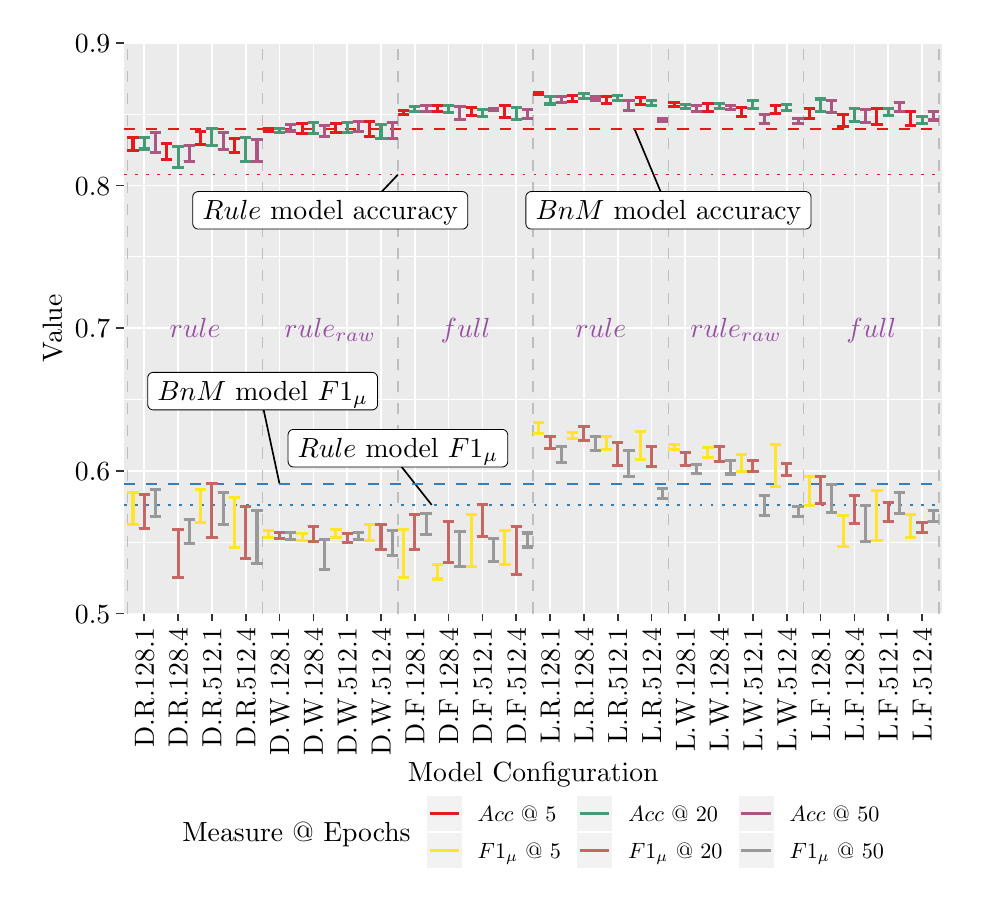
\begin{tikzpicture}[x=1pt,y=1pt]
\definecolor{fillColor}{RGB}{255,255,255}
\path[use as bounding box,fill=fillColor,fill opacity=0.00] (0,0) rectangle (336.00,311.47);
\begin{scope}
\path[clip] (  0.00,  0.00) rectangle (336.00,311.47);
\definecolor{drawColor}{RGB}{255,255,255}
\definecolor{fillColor}{RGB}{255,255,255}

\path[draw=drawColor,line width= 0.6pt,line join=round,line cap=round,fill=fillColor] (  0.00,  0.00) rectangle (336.00,311.47);
\end{scope}
\begin{scope}
\path[clip] ( 34.81, 99.77) rectangle (330.50,305.97);
\definecolor{fillColor}{gray}{0.92}

\path[fill=fillColor] ( 34.81, 99.77) rectangle (330.50,305.97);
\definecolor{drawColor}{RGB}{255,255,255}

\path[draw=drawColor,line width= 0.3pt,line join=round] ( 34.81,125.54) --
	(330.50,125.54);

\path[draw=drawColor,line width= 0.3pt,line join=round] ( 34.81,177.10) --
	(330.50,177.10);

\path[draw=drawColor,line width= 0.3pt,line join=round] ( 34.81,228.65) --
	(330.50,228.65);

\path[draw=drawColor,line width= 0.3pt,line join=round] ( 34.81,280.20) --
	(330.50,280.20);

\path[draw=drawColor,line width= 0.6pt,line join=round] ( 34.81, 99.77) --
	(330.50, 99.77);

\path[draw=drawColor,line width= 0.6pt,line join=round] ( 34.81,151.32) --
	(330.50,151.32);

\path[draw=drawColor,line width= 0.6pt,line join=round] ( 34.81,202.87) --
	(330.50,202.87);

\path[draw=drawColor,line width= 0.6pt,line join=round] ( 34.81,254.42) --
	(330.50,254.42);

\path[draw=drawColor,line width= 0.6pt,line join=round] ( 34.81,305.97) --
	(330.50,305.97);

\path[draw=drawColor,line width= 0.6pt,line join=round] ( 42.14, 99.77) --
	( 42.14,305.97);

\path[draw=drawColor,line width= 0.6pt,line join=round] ( 54.36, 99.77) --
	( 54.36,305.97);

\path[draw=drawColor,line width= 0.6pt,line join=round] ( 66.57, 99.77) --
	( 66.57,305.97);

\path[draw=drawColor,line width= 0.6pt,line join=round] ( 78.79, 99.77) --
	( 78.79,305.97);

\path[draw=drawColor,line width= 0.6pt,line join=round] ( 91.01, 99.77) --
	( 91.01,305.97);

\path[draw=drawColor,line width= 0.6pt,line join=round] (103.23, 99.77) --
	(103.23,305.97);

\path[draw=drawColor,line width= 0.6pt,line join=round] (115.45, 99.77) --
	(115.45,305.97);

\path[draw=drawColor,line width= 0.6pt,line join=round] (127.67, 99.77) --
	(127.67,305.97);

\path[draw=drawColor,line width= 0.6pt,line join=round] (139.89, 99.77) --
	(139.89,305.97);

\path[draw=drawColor,line width= 0.6pt,line join=round] (152.11, 99.77) --
	(152.11,305.97);

\path[draw=drawColor,line width= 0.6pt,line join=round] (164.32, 99.77) --
	(164.32,305.97);

\path[draw=drawColor,line width= 0.6pt,line join=round] (176.54, 99.77) --
	(176.54,305.97);

\path[draw=drawColor,line width= 0.6pt,line join=round] (188.76, 99.77) --
	(188.76,305.97);

\path[draw=drawColor,line width= 0.6pt,line join=round] (200.98, 99.77) --
	(200.98,305.97);

\path[draw=drawColor,line width= 0.6pt,line join=round] (213.20, 99.77) --
	(213.20,305.97);

\path[draw=drawColor,line width= 0.6pt,line join=round] (225.42, 99.77) --
	(225.42,305.97);

\path[draw=drawColor,line width= 0.6pt,line join=round] (237.64, 99.77) --
	(237.64,305.97);

\path[draw=drawColor,line width= 0.6pt,line join=round] (249.86, 99.77) --
	(249.86,305.97);

\path[draw=drawColor,line width= 0.6pt,line join=round] (262.07, 99.77) --
	(262.07,305.97);

\path[draw=drawColor,line width= 0.6pt,line join=round] (274.29, 99.77) --
	(274.29,305.97);

\path[draw=drawColor,line width= 0.6pt,line join=round] (286.51, 99.77) --
	(286.51,305.97);

\path[draw=drawColor,line width= 0.6pt,line join=round] (298.73, 99.77) --
	(298.73,305.97);

\path[draw=drawColor,line width= 0.6pt,line join=round] (310.95, 99.77) --
	(310.95,305.97);

\path[draw=drawColor,line width= 0.6pt,line join=round] (323.17, 99.77) --
	(323.17,305.97);
\definecolor{drawColor}{RGB}{190,190,190}

\path[draw=drawColor,line width= 0.6pt,dash pattern=on 4pt off 4pt ,line join=round] ( 36.03, 99.77) -- ( 36.03,305.97);

\path[draw=drawColor,line width= 0.6pt,dash pattern=on 4pt off 4pt ,line join=round] ( 84.90, 99.77) -- ( 84.90,305.97);

\path[draw=drawColor,line width= 0.6pt,dash pattern=on 4pt off 4pt ,line join=round] (133.78, 99.77) -- (133.78,305.97);

\path[draw=drawColor,line width= 0.6pt,dash pattern=on 4pt off 4pt ,line join=round] (182.65, 99.77) -- (182.65,305.97);

\path[draw=drawColor,line width= 0.6pt,dash pattern=on 4pt off 4pt ,line join=round] (231.53, 99.77) -- (231.53,305.97);

\path[draw=drawColor,line width= 0.6pt,dash pattern=on 4pt off 4pt ,line join=round] (280.40, 99.77) -- (280.40,305.97);

\path[draw=drawColor,line width= 0.6pt,dash pattern=on 4pt off 4pt ,line join=round] (329.28, 99.77) -- (329.28,305.97);
\definecolor{drawColor}{RGB}{152,78,163}

\node[text=drawColor,anchor=base,inner sep=0pt, outer sep=0pt, scale=  1.00] at ( 60.47,199.41) {\(rule\)};

\node[text=drawColor,anchor=base,inner sep=0pt, outer sep=0pt, scale=  1.00] at (109.34,199.41) {\(rule_{raw}\)};

\node[text=drawColor,anchor=base,inner sep=0pt, outer sep=0pt, scale=  1.00] at (158.22,199.41) {\(full\)};

\node[text=drawColor,anchor=base,inner sep=0pt, outer sep=0pt, scale=  1.00] at (207.09,199.41) {\(rule\)};

\node[text=drawColor,anchor=base,inner sep=0pt, outer sep=0pt, scale=  1.00] at (255.97,199.41) {\(rule_{raw}\)};

\node[text=drawColor,anchor=base,inner sep=0pt, outer sep=0pt, scale=  1.00] at (304.84,199.41) {\(full\)};
\definecolor{drawColor}{RGB}{0,0,0}

\path[draw=drawColor,line width= 0.6pt,line join=round] (121.56,245.47) --
	(133.78,258.36);

\path[draw=drawColor,line width= 0.6pt,line join=round] (219.31,274.78) --
	(231.53,245.47);

\path[draw=drawColor,line width= 0.6pt,line join=round] (133.78,154.47) --
	(146.00,139.01);

\path[draw=drawColor,line width= 0.6pt,line join=round] ( 84.90,175.09) --
	( 91.01,146.62);
\definecolor{fillColor}{RGB}{255,255,255}

\path[draw=drawColor,line width= 0.3pt,line join=round,line cap=round,fill=fillColor] ( 45.37,173.36) --
	(124.43,173.36) --
	(124.35,173.36) --
	(124.67,173.37) --
	(124.99,173.44) --
	(125.29,173.55) --
	(125.56,173.71) --
	(125.81,173.91) --
	(126.02,174.15) --
	(126.19,174.42) --
	(126.32,174.72) --
	(126.40,175.03) --
	(126.42,175.35) --
	(126.42,175.35) --
	(126.42,184.91) --
	(126.42,184.91) --
	(126.40,185.23) --
	(126.32,185.54) --
	(126.19,185.83) --
	(126.02,186.10) --
	(125.81,186.34) --
	(125.56,186.55) --
	(125.29,186.71) --
	(124.99,186.82) --
	(124.67,186.88) --
	(124.43,186.90) --
	( 45.37,186.90) --
	( 45.61,186.88) --
	( 45.29,186.90) --
	( 44.97,186.86) --
	( 44.67,186.77) --
	( 44.38,186.63) --
	( 44.11,186.45) --
	( 43.88,186.23) --
	( 43.69,185.97) --
	( 43.54,185.69) --
	( 43.44,185.39) --
	( 43.39,185.07) --
	( 43.38,184.91) --
	( 43.38,175.35) --
	( 43.39,175.51) --
	( 43.39,175.19) --
	( 43.44,174.87) --
	( 43.54,174.57) --
	( 43.69,174.28) --
	( 43.88,174.03) --
	( 44.11,173.81) --
	( 44.38,173.62) --
	( 44.67,173.49) --
	( 44.97,173.40) --
	( 45.29,173.36) --
	cycle;
\end{scope}
\begin{scope}
\path[clip] ( 34.81, 99.77) rectangle (330.50,305.97);
\definecolor{drawColor}{RGB}{0,0,0}

\node[text=drawColor,anchor=base,inner sep=0pt, outer sep=0pt, scale=  1.00] at ( 84.90,176.67) {\(BnM\) model \(F1_\mu\)};
\definecolor{fillColor}{RGB}{255,255,255}

\path[draw=drawColor,line width= 0.3pt,line join=round,line cap=round,fill=fillColor] ( 96.08,152.74) --
	(171.48,152.74) --
	(171.40,152.74) --
	(171.72,152.75) --
	(172.03,152.82) --
	(172.33,152.93) --
	(172.61,153.09) --
	(172.85,153.29) --
	(173.07,153.53) --
	(173.24,153.80) --
	(173.36,154.10) --
	(173.44,154.41) --
	(173.47,154.73) --
	(173.47,154.73) --
	(173.47,164.29) --
	(173.47,164.29) --
	(173.44,164.61) --
	(173.36,164.92) --
	(173.24,165.21) --
	(173.07,165.48) --
	(172.85,165.72) --
	(172.61,165.93) --
	(172.33,166.09) --
	(172.03,166.20) --
	(171.72,166.26) --
	(171.48,166.28) --
	( 96.08,166.28) --
	( 96.32,166.26) --
	( 96.00,166.28) --
	( 95.68,166.24) --
	( 95.37,166.15) --
	( 95.08,166.01) --
	( 94.82,165.83) --
	( 94.59,165.61) --
	( 94.40,165.35) --
	( 94.25,165.07) --
	( 94.15,164.77) --
	( 94.10,164.45) --
	( 94.09,164.29) --
	( 94.09,154.73) --
	( 94.10,154.89) --
	( 94.10,154.57) --
	( 94.15,154.25) --
	( 94.25,153.95) --
	( 94.40,153.66) --
	( 94.59,153.41) --
	( 94.82,153.19) --
	( 95.08,153.00) --
	( 95.37,152.87) --
	( 95.68,152.78) --
	( 96.00,152.74) --
	cycle;
\end{scope}
\begin{scope}
\path[clip] ( 34.81, 99.77) rectangle (330.50,305.97);
\definecolor{drawColor}{RGB}{0,0,0}

\node[text=drawColor,anchor=base,inner sep=0pt, outer sep=0pt, scale=  1.00] at (133.78,156.05) {\(Rule\) model \(F1_\mu\)};
\definecolor{fillColor}{RGB}{255,255,255}

\path[draw=drawColor,line width= 0.3pt,line join=round,line cap=round,fill=fillColor] ( 61.65,238.70) --
	(157.03,238.70) --
	(156.95,238.70) --
	(157.27,238.72) --
	(157.58,238.78) --
	(157.88,238.89) --
	(158.16,239.05) --
	(158.40,239.26) --
	(158.62,239.50) --
	(158.79,239.77) --
	(158.91,240.06) --
	(158.99,240.37) --
	(159.01,240.69) --
	(159.01,240.69) --
	(159.01,250.25) --
	(159.01,250.25) --
	(158.99,250.57) --
	(158.91,250.88) --
	(158.79,251.18) --
	(158.62,251.45) --
	(158.40,251.69) --
	(158.16,251.89) --
	(157.88,252.05) --
	(157.58,252.16) --
	(157.27,252.23) --
	(157.03,252.24) --
	( 61.65,252.24) --
	( 61.89,252.23) --
	( 61.57,252.24) --
	( 61.26,252.20) --
	( 60.95,252.11) --
	( 60.66,251.97) --
	( 60.40,251.79) --
	( 60.17,251.57) --
	( 59.97,251.32) --
	( 59.83,251.03) --
	( 59.72,250.73) --
	( 59.67,250.41) --
	( 59.67,250.25) --
	( 59.67,240.69) --
	( 59.67,240.85) --
	( 59.67,240.53) --
	( 59.72,240.21) --
	( 59.83,239.91) --
	( 59.97,239.63) --
	( 60.17,239.37) --
	( 60.40,239.15) --
	( 60.66,238.97) --
	( 60.95,238.83) --
	( 61.26,238.74) --
	( 61.57,238.70) --
	cycle;
\end{scope}
\begin{scope}
\path[clip] ( 34.81, 99.77) rectangle (330.50,305.97);
\definecolor{drawColor}{RGB}{0,0,0}

\node[text=drawColor,anchor=base,inner sep=0pt, outer sep=0pt, scale=  1.00] at (109.34,242.01) {\(Rule\) model accuracy};
\definecolor{fillColor}{RGB}{255,255,255}

\path[draw=drawColor,line width= 0.3pt,line join=round,line cap=round,fill=fillColor] (182.01,238.70) --
	(281.05,238.70) --
	(280.97,238.70) --
	(281.29,238.72) --
	(281.60,238.78) --
	(281.90,238.89) --
	(282.17,239.05) --
	(282.42,239.26) --
	(282.63,239.50) --
	(282.81,239.77) --
	(282.93,240.06) --
	(283.01,240.37) --
	(283.03,240.69) --
	(283.03,240.69) --
	(283.03,250.25) --
	(283.03,250.25) --
	(283.01,250.57) --
	(282.93,250.88) --
	(282.81,251.18) --
	(282.63,251.45) --
	(282.42,251.69) --
	(282.17,251.89) --
	(281.90,252.05) --
	(281.60,252.16) --
	(281.29,252.23) --
	(281.05,252.24) --
	(182.01,252.24) --
	(182.25,252.23) --
	(181.93,252.24) --
	(181.61,252.20) --
	(181.31,252.11) --
	(181.02,251.97) --
	(180.75,251.79) --
	(180.52,251.57) --
	(180.33,251.32) --
	(180.18,251.03) --
	(180.08,250.73) --
	(180.03,250.41) --
	(180.02,250.25) --
	(180.02,240.69) --
	(180.03,240.85) --
	(180.03,240.53) --
	(180.08,240.21) --
	(180.18,239.91) --
	(180.33,239.63) --
	(180.52,239.37) --
	(180.75,239.15) --
	(181.02,238.97) --
	(181.31,238.83) --
	(181.61,238.74) --
	(181.93,238.70) --
	cycle;
\end{scope}
\begin{scope}
\path[clip] ( 34.81, 99.77) rectangle (330.50,305.97);
\definecolor{drawColor}{RGB}{0,0,0}

\node[text=drawColor,anchor=base,inner sep=0pt, outer sep=0pt, scale=  1.00] at (231.53,242.01) {\(BnM\) model accuracy};
\definecolor{drawColor}{RGB}{228,26,28}

\path[draw=drawColor,line width= 0.6pt,dash pattern=on 4pt off 4pt ,line join=round] ( 34.81,274.78) -- (330.50,274.78);

\path[draw=drawColor,line width= 0.6pt,dash pattern=on 1pt off 3pt ,line join=round] ( 34.81,258.36) -- (330.50,258.36);
\definecolor{drawColor}{RGB}{55,126,184}

\path[draw=drawColor,line width= 0.6pt,dash pattern=on 4pt off 4pt ,line join=round] ( 34.81,146.62) -- (330.50,146.62);

\path[draw=drawColor,line width= 0.6pt,dash pattern=on 1pt off 3pt ,line join=round] ( 34.81,139.01) -- (330.50,139.01);
\definecolor{drawColor}{RGB}{172,87,130}

\path[draw=drawColor,line width= 1.1pt,line join=round] ( 44.17,273.65) --
	( 48.25,273.65);

\path[draw=drawColor,line width= 1.1pt,line join=round] ( 46.21,273.65) --
	( 46.21,266.20);

\path[draw=drawColor,line width= 1.1pt,line join=round] ( 44.17,266.20) --
	( 48.25,266.20);

\path[draw=drawColor,line width= 1.1pt,line join=round] ( 44.17,273.65) --
	( 48.25,273.65);

\path[draw=drawColor,line width= 1.1pt,line join=round] ( 46.21,273.65) --
	( 46.21,266.20);

\path[draw=drawColor,line width= 1.1pt,line join=round] ( 44.17,266.20) --
	( 48.25,266.20);

\path[draw=drawColor,line width= 1.1pt,line join=round] ( 44.17,273.65) --
	( 48.25,273.65);

\path[draw=drawColor,line width= 1.1pt,line join=round] ( 46.21,273.65) --
	( 46.21,266.20);

\path[draw=drawColor,line width= 1.1pt,line join=round] ( 44.17,266.20) --
	( 48.25,266.20);

\path[draw=drawColor,line width= 1.1pt,line join=round] ( 44.17,273.65) --
	( 48.25,273.65);

\path[draw=drawColor,line width= 1.1pt,line join=round] ( 46.21,273.65) --
	( 46.21,266.20);

\path[draw=drawColor,line width= 1.1pt,line join=round] ( 44.17,266.20) --
	( 48.25,266.20);

\path[draw=drawColor,line width= 1.1pt,line join=round] ( 44.17,273.65) --
	( 48.25,273.65);

\path[draw=drawColor,line width= 1.1pt,line join=round] ( 46.21,273.65) --
	( 46.21,266.20);

\path[draw=drawColor,line width= 1.1pt,line join=round] ( 44.17,266.20) --
	( 48.25,266.20);

\path[draw=drawColor,line width= 1.1pt,line join=round] ( 44.17,273.65) --
	( 48.25,273.65);

\path[draw=drawColor,line width= 1.1pt,line join=round] ( 46.21,273.65) --
	( 46.21,266.20);

\path[draw=drawColor,line width= 1.1pt,line join=round] ( 44.17,266.20) --
	( 48.25,266.20);

\path[draw=drawColor,line width= 1.1pt,line join=round] ( 44.17,273.65) --
	( 48.25,273.65);

\path[draw=drawColor,line width= 1.1pt,line join=round] ( 46.21,273.65) --
	( 46.21,266.20);

\path[draw=drawColor,line width= 1.1pt,line join=round] ( 44.17,266.20) --
	( 48.25,266.20);

\path[draw=drawColor,line width= 1.1pt,line join=round] ( 44.17,273.65) --
	( 48.25,273.65);

\path[draw=drawColor,line width= 1.1pt,line join=round] ( 46.21,273.65) --
	( 46.21,266.20);

\path[draw=drawColor,line width= 1.1pt,line join=round] ( 44.17,266.20) --
	( 48.25,266.20);
\definecolor{drawColor}{RGB}{68,155,117}

\path[draw=drawColor,line width= 1.1pt,line join=round] ( 40.10,271.74) --
	( 44.17,271.74);

\path[draw=drawColor,line width= 1.1pt,line join=round] ( 42.14,271.74) --
	( 42.14,267.63);

\path[draw=drawColor,line width= 1.1pt,line join=round] ( 40.10,267.63) --
	( 44.17,267.63);

\path[draw=drawColor,line width= 1.1pt,line join=round] ( 40.10,271.74) --
	( 44.17,271.74);

\path[draw=drawColor,line width= 1.1pt,line join=round] ( 42.14,271.74) --
	( 42.14,267.63);

\path[draw=drawColor,line width= 1.1pt,line join=round] ( 40.10,267.63) --
	( 44.17,267.63);

\path[draw=drawColor,line width= 1.1pt,line join=round] ( 40.10,271.74) --
	( 44.17,271.74);

\path[draw=drawColor,line width= 1.1pt,line join=round] ( 42.14,271.74) --
	( 42.14,267.63);

\path[draw=drawColor,line width= 1.1pt,line join=round] ( 40.10,267.63) --
	( 44.17,267.63);

\path[draw=drawColor,line width= 1.1pt,line join=round] ( 40.10,271.74) --
	( 44.17,271.74);

\path[draw=drawColor,line width= 1.1pt,line join=round] ( 42.14,271.74) --
	( 42.14,267.63);

\path[draw=drawColor,line width= 1.1pt,line join=round] ( 40.10,267.63) --
	( 44.17,267.63);

\path[draw=drawColor,line width= 1.1pt,line join=round] ( 40.10,271.74) --
	( 44.17,271.74);

\path[draw=drawColor,line width= 1.1pt,line join=round] ( 42.14,271.74) --
	( 42.14,267.63);

\path[draw=drawColor,line width= 1.1pt,line join=round] ( 40.10,267.63) --
	( 44.17,267.63);

\path[draw=drawColor,line width= 1.1pt,line join=round] ( 40.10,271.74) --
	( 44.17,271.74);

\path[draw=drawColor,line width= 1.1pt,line join=round] ( 42.14,271.74) --
	( 42.14,267.63);

\path[draw=drawColor,line width= 1.1pt,line join=round] ( 40.10,267.63) --
	( 44.17,267.63);

\path[draw=drawColor,line width= 1.1pt,line join=round] ( 40.10,271.74) --
	( 44.17,271.74);

\path[draw=drawColor,line width= 1.1pt,line join=round] ( 42.14,271.74) --
	( 42.14,267.63);

\path[draw=drawColor,line width= 1.1pt,line join=round] ( 40.10,267.63) --
	( 44.17,267.63);

\path[draw=drawColor,line width= 1.1pt,line join=round] ( 40.10,271.74) --
	( 44.17,271.74);

\path[draw=drawColor,line width= 1.1pt,line join=round] ( 42.14,271.74) --
	( 42.14,267.63);

\path[draw=drawColor,line width= 1.1pt,line join=round] ( 40.10,267.63) --
	( 44.17,267.63);
\definecolor{drawColor}{RGB}{228,26,28}

\path[draw=drawColor,line width= 1.1pt,line join=round] ( 36.03,271.71) --
	( 40.10,271.71);

\path[draw=drawColor,line width= 1.1pt,line join=round] ( 38.06,271.71) --
	( 38.06,267.11);

\path[draw=drawColor,line width= 1.1pt,line join=round] ( 36.03,267.11) --
	( 40.10,267.11);

\path[draw=drawColor,line width= 1.1pt,line join=round] ( 36.03,271.71) --
	( 40.10,271.71);

\path[draw=drawColor,line width= 1.1pt,line join=round] ( 38.06,271.71) --
	( 38.06,267.11);

\path[draw=drawColor,line width= 1.1pt,line join=round] ( 36.03,267.11) --
	( 40.10,267.11);

\path[draw=drawColor,line width= 1.1pt,line join=round] ( 36.03,271.71) --
	( 40.10,271.71);

\path[draw=drawColor,line width= 1.1pt,line join=round] ( 38.06,271.71) --
	( 38.06,267.11);

\path[draw=drawColor,line width= 1.1pt,line join=round] ( 36.03,267.11) --
	( 40.10,267.11);

\path[draw=drawColor,line width= 1.1pt,line join=round] ( 36.03,271.71) --
	( 40.10,271.71);

\path[draw=drawColor,line width= 1.1pt,line join=round] ( 38.06,271.71) --
	( 38.06,267.11);

\path[draw=drawColor,line width= 1.1pt,line join=round] ( 36.03,267.11) --
	( 40.10,267.11);

\path[draw=drawColor,line width= 1.1pt,line join=round] ( 36.03,271.71) --
	( 40.10,271.71);

\path[draw=drawColor,line width= 1.1pt,line join=round] ( 38.06,271.71) --
	( 38.06,267.11);

\path[draw=drawColor,line width= 1.1pt,line join=round] ( 36.03,267.11) --
	( 40.10,267.11);

\path[draw=drawColor,line width= 1.1pt,line join=round] ( 36.03,271.71) --
	( 40.10,271.71);

\path[draw=drawColor,line width= 1.1pt,line join=round] ( 38.06,271.71) --
	( 38.06,267.11);

\path[draw=drawColor,line width= 1.1pt,line join=round] ( 36.03,267.11) --
	( 40.10,267.11);

\path[draw=drawColor,line width= 1.1pt,line join=round] ( 36.03,271.71) --
	( 40.10,271.71);

\path[draw=drawColor,line width= 1.1pt,line join=round] ( 38.06,271.71) --
	( 38.06,267.11);

\path[draw=drawColor,line width= 1.1pt,line join=round] ( 36.03,267.11) --
	( 40.10,267.11);

\path[draw=drawColor,line width= 1.1pt,line join=round] ( 36.03,271.71) --
	( 40.10,271.71);

\path[draw=drawColor,line width= 1.1pt,line join=round] ( 38.06,271.71) --
	( 38.06,267.11);

\path[draw=drawColor,line width= 1.1pt,line join=round] ( 36.03,267.11) --
	( 40.10,267.11);
\definecolor{drawColor}{RGB}{172,87,130}

\path[draw=drawColor,line width= 1.1pt,line join=round] ( 56.39,269.00) --
	( 60.47,269.00);

\path[draw=drawColor,line width= 1.1pt,line join=round] ( 58.43,269.00) --
	( 58.43,263.17);

\path[draw=drawColor,line width= 1.1pt,line join=round] ( 56.39,263.17) --
	( 60.47,263.17);

\path[draw=drawColor,line width= 1.1pt,line join=round] ( 56.39,269.00) --
	( 60.47,269.00);

\path[draw=drawColor,line width= 1.1pt,line join=round] ( 58.43,269.00) --
	( 58.43,263.17);

\path[draw=drawColor,line width= 1.1pt,line join=round] ( 56.39,263.17) --
	( 60.47,263.17);

\path[draw=drawColor,line width= 1.1pt,line join=round] ( 56.39,269.00) --
	( 60.47,269.00);

\path[draw=drawColor,line width= 1.1pt,line join=round] ( 58.43,269.00) --
	( 58.43,263.17);

\path[draw=drawColor,line width= 1.1pt,line join=round] ( 56.39,263.17) --
	( 60.47,263.17);

\path[draw=drawColor,line width= 1.1pt,line join=round] ( 56.39,269.00) --
	( 60.47,269.00);

\path[draw=drawColor,line width= 1.1pt,line join=round] ( 58.43,269.00) --
	( 58.43,263.17);

\path[draw=drawColor,line width= 1.1pt,line join=round] ( 56.39,263.17) --
	( 60.47,263.17);

\path[draw=drawColor,line width= 1.1pt,line join=round] ( 56.39,269.00) --
	( 60.47,269.00);

\path[draw=drawColor,line width= 1.1pt,line join=round] ( 58.43,269.00) --
	( 58.43,263.17);

\path[draw=drawColor,line width= 1.1pt,line join=round] ( 56.39,263.17) --
	( 60.47,263.17);

\path[draw=drawColor,line width= 1.1pt,line join=round] ( 56.39,269.00) --
	( 60.47,269.00);

\path[draw=drawColor,line width= 1.1pt,line join=round] ( 58.43,269.00) --
	( 58.43,263.17);

\path[draw=drawColor,line width= 1.1pt,line join=round] ( 56.39,263.17) --
	( 60.47,263.17);

\path[draw=drawColor,line width= 1.1pt,line join=round] ( 56.39,269.00) --
	( 60.47,269.00);

\path[draw=drawColor,line width= 1.1pt,line join=round] ( 58.43,269.00) --
	( 58.43,263.17);

\path[draw=drawColor,line width= 1.1pt,line join=round] ( 56.39,263.17) --
	( 60.47,263.17);

\path[draw=drawColor,line width= 1.1pt,line join=round] ( 56.39,269.00) --
	( 60.47,269.00);

\path[draw=drawColor,line width= 1.1pt,line join=round] ( 58.43,269.00) --
	( 58.43,263.17);

\path[draw=drawColor,line width= 1.1pt,line join=round] ( 56.39,263.17) --
	( 60.47,263.17);
\definecolor{drawColor}{RGB}{68,155,117}

\path[draw=drawColor,line width= 1.1pt,line join=round] ( 52.32,268.59) --
	( 56.39,268.59);

\path[draw=drawColor,line width= 1.1pt,line join=round] ( 54.36,268.59) --
	( 54.36,261.01);

\path[draw=drawColor,line width= 1.1pt,line join=round] ( 52.32,261.01) --
	( 56.39,261.01);

\path[draw=drawColor,line width= 1.1pt,line join=round] ( 52.32,268.59) --
	( 56.39,268.59);

\path[draw=drawColor,line width= 1.1pt,line join=round] ( 54.36,268.59) --
	( 54.36,261.01);

\path[draw=drawColor,line width= 1.1pt,line join=round] ( 52.32,261.01) --
	( 56.39,261.01);

\path[draw=drawColor,line width= 1.1pt,line join=round] ( 52.32,268.59) --
	( 56.39,268.59);

\path[draw=drawColor,line width= 1.1pt,line join=round] ( 54.36,268.59) --
	( 54.36,261.01);

\path[draw=drawColor,line width= 1.1pt,line join=round] ( 52.32,261.01) --
	( 56.39,261.01);

\path[draw=drawColor,line width= 1.1pt,line join=round] ( 52.32,268.59) --
	( 56.39,268.59);

\path[draw=drawColor,line width= 1.1pt,line join=round] ( 54.36,268.59) --
	( 54.36,261.01);

\path[draw=drawColor,line width= 1.1pt,line join=round] ( 52.32,261.01) --
	( 56.39,261.01);

\path[draw=drawColor,line width= 1.1pt,line join=round] ( 52.32,268.59) --
	( 56.39,268.59);

\path[draw=drawColor,line width= 1.1pt,line join=round] ( 54.36,268.59) --
	( 54.36,261.01);

\path[draw=drawColor,line width= 1.1pt,line join=round] ( 52.32,261.01) --
	( 56.39,261.01);

\path[draw=drawColor,line width= 1.1pt,line join=round] ( 52.32,268.59) --
	( 56.39,268.59);

\path[draw=drawColor,line width= 1.1pt,line join=round] ( 54.36,268.59) --
	( 54.36,261.01);

\path[draw=drawColor,line width= 1.1pt,line join=round] ( 52.32,261.01) --
	( 56.39,261.01);

\path[draw=drawColor,line width= 1.1pt,line join=round] ( 52.32,268.59) --
	( 56.39,268.59);

\path[draw=drawColor,line width= 1.1pt,line join=round] ( 54.36,268.59) --
	( 54.36,261.01);

\path[draw=drawColor,line width= 1.1pt,line join=round] ( 52.32,261.01) --
	( 56.39,261.01);

\path[draw=drawColor,line width= 1.1pt,line join=round] ( 52.32,268.59) --
	( 56.39,268.59);

\path[draw=drawColor,line width= 1.1pt,line join=round] ( 54.36,268.59) --
	( 54.36,261.01);

\path[draw=drawColor,line width= 1.1pt,line join=round] ( 52.32,261.01) --
	( 56.39,261.01);
\definecolor{drawColor}{RGB}{228,26,28}

\path[draw=drawColor,line width= 1.1pt,line join=round] ( 48.25,269.65) --
	( 52.32,269.65);

\path[draw=drawColor,line width= 1.1pt,line join=round] ( 50.28,269.65) --
	( 50.28,263.71);

\path[draw=drawColor,line width= 1.1pt,line join=round] ( 48.25,263.71) --
	( 52.32,263.71);

\path[draw=drawColor,line width= 1.1pt,line join=round] ( 48.25,269.65) --
	( 52.32,269.65);

\path[draw=drawColor,line width= 1.1pt,line join=round] ( 50.28,269.65) --
	( 50.28,263.71);

\path[draw=drawColor,line width= 1.1pt,line join=round] ( 48.25,263.71) --
	( 52.32,263.71);

\path[draw=drawColor,line width= 1.1pt,line join=round] ( 48.25,269.65) --
	( 52.32,269.65);

\path[draw=drawColor,line width= 1.1pt,line join=round] ( 50.28,269.65) --
	( 50.28,263.71);

\path[draw=drawColor,line width= 1.1pt,line join=round] ( 48.25,263.71) --
	( 52.32,263.71);

\path[draw=drawColor,line width= 1.1pt,line join=round] ( 48.25,269.65) --
	( 52.32,269.65);

\path[draw=drawColor,line width= 1.1pt,line join=round] ( 50.28,269.65) --
	( 50.28,263.71);

\path[draw=drawColor,line width= 1.1pt,line join=round] ( 48.25,263.71) --
	( 52.32,263.71);

\path[draw=drawColor,line width= 1.1pt,line join=round] ( 48.25,269.65) --
	( 52.32,269.65);

\path[draw=drawColor,line width= 1.1pt,line join=round] ( 50.28,269.65) --
	( 50.28,263.71);

\path[draw=drawColor,line width= 1.1pt,line join=round] ( 48.25,263.71) --
	( 52.32,263.71);

\path[draw=drawColor,line width= 1.1pt,line join=round] ( 48.25,269.65) --
	( 52.32,269.65);

\path[draw=drawColor,line width= 1.1pt,line join=round] ( 50.28,269.65) --
	( 50.28,263.71);

\path[draw=drawColor,line width= 1.1pt,line join=round] ( 48.25,263.71) --
	( 52.32,263.71);

\path[draw=drawColor,line width= 1.1pt,line join=round] ( 48.25,269.65) --
	( 52.32,269.65);

\path[draw=drawColor,line width= 1.1pt,line join=round] ( 50.28,269.65) --
	( 50.28,263.71);

\path[draw=drawColor,line width= 1.1pt,line join=round] ( 48.25,263.71) --
	( 52.32,263.71);

\path[draw=drawColor,line width= 1.1pt,line join=round] ( 48.25,269.65) --
	( 52.32,269.65);

\path[draw=drawColor,line width= 1.1pt,line join=round] ( 50.28,269.65) --
	( 50.28,263.71);

\path[draw=drawColor,line width= 1.1pt,line join=round] ( 48.25,263.71) --
	( 52.32,263.71);
\definecolor{drawColor}{RGB}{172,87,130}

\path[draw=drawColor,line width= 1.1pt,line join=round] ( 68.61,273.53) --
	( 72.68,273.53);

\path[draw=drawColor,line width= 1.1pt,line join=round] ( 70.65,273.53) --
	( 70.65,267.33);

\path[draw=drawColor,line width= 1.1pt,line join=round] ( 68.61,267.33) --
	( 72.68,267.33);

\path[draw=drawColor,line width= 1.1pt,line join=round] ( 68.61,273.53) --
	( 72.68,273.53);

\path[draw=drawColor,line width= 1.1pt,line join=round] ( 70.65,273.53) --
	( 70.65,267.33);

\path[draw=drawColor,line width= 1.1pt,line join=round] ( 68.61,267.33) --
	( 72.68,267.33);

\path[draw=drawColor,line width= 1.1pt,line join=round] ( 68.61,273.53) --
	( 72.68,273.53);

\path[draw=drawColor,line width= 1.1pt,line join=round] ( 70.65,273.53) --
	( 70.65,267.33);

\path[draw=drawColor,line width= 1.1pt,line join=round] ( 68.61,267.33) --
	( 72.68,267.33);

\path[draw=drawColor,line width= 1.1pt,line join=round] ( 68.61,273.53) --
	( 72.68,273.53);

\path[draw=drawColor,line width= 1.1pt,line join=round] ( 70.65,273.53) --
	( 70.65,267.33);

\path[draw=drawColor,line width= 1.1pt,line join=round] ( 68.61,267.33) --
	( 72.68,267.33);

\path[draw=drawColor,line width= 1.1pt,line join=round] ( 68.61,273.53) --
	( 72.68,273.53);

\path[draw=drawColor,line width= 1.1pt,line join=round] ( 70.65,273.53) --
	( 70.65,267.33);

\path[draw=drawColor,line width= 1.1pt,line join=round] ( 68.61,267.33) --
	( 72.68,267.33);

\path[draw=drawColor,line width= 1.1pt,line join=round] ( 68.61,273.53) --
	( 72.68,273.53);

\path[draw=drawColor,line width= 1.1pt,line join=round] ( 70.65,273.53) --
	( 70.65,267.33);

\path[draw=drawColor,line width= 1.1pt,line join=round] ( 68.61,267.33) --
	( 72.68,267.33);

\path[draw=drawColor,line width= 1.1pt,line join=round] ( 68.61,273.53) --
	( 72.68,273.53);

\path[draw=drawColor,line width= 1.1pt,line join=round] ( 70.65,273.53) --
	( 70.65,267.33);

\path[draw=drawColor,line width= 1.1pt,line join=round] ( 68.61,267.33) --
	( 72.68,267.33);

\path[draw=drawColor,line width= 1.1pt,line join=round] ( 68.61,273.53) --
	( 72.68,273.53);

\path[draw=drawColor,line width= 1.1pt,line join=round] ( 70.65,273.53) --
	( 70.65,267.33);

\path[draw=drawColor,line width= 1.1pt,line join=round] ( 68.61,267.33) --
	( 72.68,267.33);
\definecolor{drawColor}{RGB}{68,155,117}

\path[draw=drawColor,line width= 1.1pt,line join=round] ( 64.54,274.95) --
	( 68.61,274.95);

\path[draw=drawColor,line width= 1.1pt,line join=round] ( 66.57,274.95) --
	( 66.57,268.85);

\path[draw=drawColor,line width= 1.1pt,line join=round] ( 64.54,268.85) --
	( 68.61,268.85);

\path[draw=drawColor,line width= 1.1pt,line join=round] ( 64.54,274.95) --
	( 68.61,274.95);

\path[draw=drawColor,line width= 1.1pt,line join=round] ( 66.57,274.95) --
	( 66.57,268.85);

\path[draw=drawColor,line width= 1.1pt,line join=round] ( 64.54,268.85) --
	( 68.61,268.85);

\path[draw=drawColor,line width= 1.1pt,line join=round] ( 64.54,274.95) --
	( 68.61,274.95);

\path[draw=drawColor,line width= 1.1pt,line join=round] ( 66.57,274.95) --
	( 66.57,268.85);

\path[draw=drawColor,line width= 1.1pt,line join=round] ( 64.54,268.85) --
	( 68.61,268.85);

\path[draw=drawColor,line width= 1.1pt,line join=round] ( 64.54,274.95) --
	( 68.61,274.95);

\path[draw=drawColor,line width= 1.1pt,line join=round] ( 66.57,274.95) --
	( 66.57,268.85);

\path[draw=drawColor,line width= 1.1pt,line join=round] ( 64.54,268.85) --
	( 68.61,268.85);

\path[draw=drawColor,line width= 1.1pt,line join=round] ( 64.54,274.95) --
	( 68.61,274.95);

\path[draw=drawColor,line width= 1.1pt,line join=round] ( 66.57,274.95) --
	( 66.57,268.85);

\path[draw=drawColor,line width= 1.1pt,line join=round] ( 64.54,268.85) --
	( 68.61,268.85);

\path[draw=drawColor,line width= 1.1pt,line join=round] ( 64.54,274.95) --
	( 68.61,274.95);

\path[draw=drawColor,line width= 1.1pt,line join=round] ( 66.57,274.95) --
	( 66.57,268.85);

\path[draw=drawColor,line width= 1.1pt,line join=round] ( 64.54,268.85) --
	( 68.61,268.85);

\path[draw=drawColor,line width= 1.1pt,line join=round] ( 64.54,274.95) --
	( 68.61,274.95);

\path[draw=drawColor,line width= 1.1pt,line join=round] ( 66.57,274.95) --
	( 66.57,268.85);

\path[draw=drawColor,line width= 1.1pt,line join=round] ( 64.54,268.85) --
	( 68.61,268.85);

\path[draw=drawColor,line width= 1.1pt,line join=round] ( 64.54,274.95) --
	( 68.61,274.95);

\path[draw=drawColor,line width= 1.1pt,line join=round] ( 66.57,274.95) --
	( 66.57,268.85);

\path[draw=drawColor,line width= 1.1pt,line join=round] ( 64.54,268.85) --
	( 68.61,268.85);
\definecolor{drawColor}{RGB}{228,26,28}

\path[draw=drawColor,line width= 1.1pt,line join=round] ( 60.47,273.98) --
	( 64.54,273.98);

\path[draw=drawColor,line width= 1.1pt,line join=round] ( 62.50,273.98) --
	( 62.50,269.16);

\path[draw=drawColor,line width= 1.1pt,line join=round] ( 60.47,269.16) --
	( 64.54,269.16);

\path[draw=drawColor,line width= 1.1pt,line join=round] ( 60.47,273.98) --
	( 64.54,273.98);

\path[draw=drawColor,line width= 1.1pt,line join=round] ( 62.50,273.98) --
	( 62.50,269.16);

\path[draw=drawColor,line width= 1.1pt,line join=round] ( 60.47,269.16) --
	( 64.54,269.16);

\path[draw=drawColor,line width= 1.1pt,line join=round] ( 60.47,273.98) --
	( 64.54,273.98);

\path[draw=drawColor,line width= 1.1pt,line join=round] ( 62.50,273.98) --
	( 62.50,269.16);

\path[draw=drawColor,line width= 1.1pt,line join=round] ( 60.47,269.16) --
	( 64.54,269.16);

\path[draw=drawColor,line width= 1.1pt,line join=round] ( 60.47,273.98) --
	( 64.54,273.98);

\path[draw=drawColor,line width= 1.1pt,line join=round] ( 62.50,273.98) --
	( 62.50,269.16);

\path[draw=drawColor,line width= 1.1pt,line join=round] ( 60.47,269.16) --
	( 64.54,269.16);

\path[draw=drawColor,line width= 1.1pt,line join=round] ( 60.47,273.98) --
	( 64.54,273.98);

\path[draw=drawColor,line width= 1.1pt,line join=round] ( 62.50,273.98) --
	( 62.50,269.16);

\path[draw=drawColor,line width= 1.1pt,line join=round] ( 60.47,269.16) --
	( 64.54,269.16);

\path[draw=drawColor,line width= 1.1pt,line join=round] ( 60.47,273.98) --
	( 64.54,273.98);

\path[draw=drawColor,line width= 1.1pt,line join=round] ( 62.50,273.98) --
	( 62.50,269.16);

\path[draw=drawColor,line width= 1.1pt,line join=round] ( 60.47,269.16) --
	( 64.54,269.16);

\path[draw=drawColor,line width= 1.1pt,line join=round] ( 60.47,273.98) --
	( 64.54,273.98);

\path[draw=drawColor,line width= 1.1pt,line join=round] ( 62.50,273.98) --
	( 62.50,269.16);

\path[draw=drawColor,line width= 1.1pt,line join=round] ( 60.47,269.16) --
	( 64.54,269.16);

\path[draw=drawColor,line width= 1.1pt,line join=round] ( 60.47,273.98) --
	( 64.54,273.98);

\path[draw=drawColor,line width= 1.1pt,line join=round] ( 62.50,273.98) --
	( 62.50,269.16);

\path[draw=drawColor,line width= 1.1pt,line join=round] ( 60.47,269.16) --
	( 64.54,269.16);
\definecolor{drawColor}{RGB}{172,87,130}

\path[draw=drawColor,line width= 1.1pt,line join=round] ( 80.83,271.04) --
	( 84.90,271.04);

\path[draw=drawColor,line width= 1.1pt,line join=round] ( 82.87,271.04) --
	( 82.87,263.06);

\path[draw=drawColor,line width= 1.1pt,line join=round] ( 80.83,263.06) --
	( 84.90,263.06);

\path[draw=drawColor,line width= 1.1pt,line join=round] ( 80.83,271.04) --
	( 84.90,271.04);

\path[draw=drawColor,line width= 1.1pt,line join=round] ( 82.87,271.04) --
	( 82.87,263.06);

\path[draw=drawColor,line width= 1.1pt,line join=round] ( 80.83,263.06) --
	( 84.90,263.06);

\path[draw=drawColor,line width= 1.1pt,line join=round] ( 80.83,271.04) --
	( 84.90,271.04);

\path[draw=drawColor,line width= 1.1pt,line join=round] ( 82.87,271.04) --
	( 82.87,263.06);

\path[draw=drawColor,line width= 1.1pt,line join=round] ( 80.83,263.06) --
	( 84.90,263.06);

\path[draw=drawColor,line width= 1.1pt,line join=round] ( 80.83,271.04) --
	( 84.90,271.04);

\path[draw=drawColor,line width= 1.1pt,line join=round] ( 82.87,271.04) --
	( 82.87,263.06);

\path[draw=drawColor,line width= 1.1pt,line join=round] ( 80.83,263.06) --
	( 84.90,263.06);

\path[draw=drawColor,line width= 1.1pt,line join=round] ( 80.83,271.04) --
	( 84.90,271.04);

\path[draw=drawColor,line width= 1.1pt,line join=round] ( 82.87,271.04) --
	( 82.87,263.06);

\path[draw=drawColor,line width= 1.1pt,line join=round] ( 80.83,263.06) --
	( 84.90,263.06);

\path[draw=drawColor,line width= 1.1pt,line join=round] ( 80.83,271.04) --
	( 84.90,271.04);

\path[draw=drawColor,line width= 1.1pt,line join=round] ( 82.87,271.04) --
	( 82.87,263.06);

\path[draw=drawColor,line width= 1.1pt,line join=round] ( 80.83,263.06) --
	( 84.90,263.06);

\path[draw=drawColor,line width= 1.1pt,line join=round] ( 80.83,271.04) --
	( 84.90,271.04);

\path[draw=drawColor,line width= 1.1pt,line join=round] ( 82.87,271.04) --
	( 82.87,263.06);

\path[draw=drawColor,line width= 1.1pt,line join=round] ( 80.83,263.06) --
	( 84.90,263.06);

\path[draw=drawColor,line width= 1.1pt,line join=round] ( 80.83,271.04) --
	( 84.90,271.04);

\path[draw=drawColor,line width= 1.1pt,line join=round] ( 82.87,271.04) --
	( 82.87,263.06);

\path[draw=drawColor,line width= 1.1pt,line join=round] ( 80.83,263.06) --
	( 84.90,263.06);
\definecolor{drawColor}{RGB}{68,155,117}

\path[draw=drawColor,line width= 1.1pt,line join=round] ( 76.76,271.70) --
	( 80.83,271.70);

\path[draw=drawColor,line width= 1.1pt,line join=round] ( 78.79,271.70) --
	( 78.79,263.24);

\path[draw=drawColor,line width= 1.1pt,line join=round] ( 76.76,263.24) --
	( 80.83,263.24);

\path[draw=drawColor,line width= 1.1pt,line join=round] ( 76.76,271.70) --
	( 80.83,271.70);

\path[draw=drawColor,line width= 1.1pt,line join=round] ( 78.79,271.70) --
	( 78.79,263.24);

\path[draw=drawColor,line width= 1.1pt,line join=round] ( 76.76,263.24) --
	( 80.83,263.24);

\path[draw=drawColor,line width= 1.1pt,line join=round] ( 76.76,271.70) --
	( 80.83,271.70);

\path[draw=drawColor,line width= 1.1pt,line join=round] ( 78.79,271.70) --
	( 78.79,263.24);

\path[draw=drawColor,line width= 1.1pt,line join=round] ( 76.76,263.24) --
	( 80.83,263.24);

\path[draw=drawColor,line width= 1.1pt,line join=round] ( 76.76,271.70) --
	( 80.83,271.70);

\path[draw=drawColor,line width= 1.1pt,line join=round] ( 78.79,271.70) --
	( 78.79,263.24);

\path[draw=drawColor,line width= 1.1pt,line join=round] ( 76.76,263.24) --
	( 80.83,263.24);

\path[draw=drawColor,line width= 1.1pt,line join=round] ( 76.76,271.70) --
	( 80.83,271.70);

\path[draw=drawColor,line width= 1.1pt,line join=round] ( 78.79,271.70) --
	( 78.79,263.24);

\path[draw=drawColor,line width= 1.1pt,line join=round] ( 76.76,263.24) --
	( 80.83,263.24);

\path[draw=drawColor,line width= 1.1pt,line join=round] ( 76.76,271.70) --
	( 80.83,271.70);

\path[draw=drawColor,line width= 1.1pt,line join=round] ( 78.79,271.70) --
	( 78.79,263.24);

\path[draw=drawColor,line width= 1.1pt,line join=round] ( 76.76,263.24) --
	( 80.83,263.24);

\path[draw=drawColor,line width= 1.1pt,line join=round] ( 76.76,271.70) --
	( 80.83,271.70);

\path[draw=drawColor,line width= 1.1pt,line join=round] ( 78.79,271.70) --
	( 78.79,263.24);

\path[draw=drawColor,line width= 1.1pt,line join=round] ( 76.76,263.24) --
	( 80.83,263.24);

\path[draw=drawColor,line width= 1.1pt,line join=round] ( 76.76,271.70) --
	( 80.83,271.70);

\path[draw=drawColor,line width= 1.1pt,line join=round] ( 78.79,271.70) --
	( 78.79,263.24);

\path[draw=drawColor,line width= 1.1pt,line join=round] ( 76.76,263.24) --
	( 80.83,263.24);
\definecolor{drawColor}{RGB}{228,26,28}

\path[draw=drawColor,line width= 1.1pt,line join=round] ( 72.68,271.48) --
	( 76.76,271.48);

\path[draw=drawColor,line width= 1.1pt,line join=round] ( 74.72,271.48) --
	( 74.72,266.29);

\path[draw=drawColor,line width= 1.1pt,line join=round] ( 72.68,266.29) --
	( 76.76,266.29);

\path[draw=drawColor,line width= 1.1pt,line join=round] ( 72.68,271.48) --
	( 76.76,271.48);

\path[draw=drawColor,line width= 1.1pt,line join=round] ( 74.72,271.48) --
	( 74.72,266.29);

\path[draw=drawColor,line width= 1.1pt,line join=round] ( 72.68,266.29) --
	( 76.76,266.29);

\path[draw=drawColor,line width= 1.1pt,line join=round] ( 72.68,271.48) --
	( 76.76,271.48);

\path[draw=drawColor,line width= 1.1pt,line join=round] ( 74.72,271.48) --
	( 74.72,266.29);

\path[draw=drawColor,line width= 1.1pt,line join=round] ( 72.68,266.29) --
	( 76.76,266.29);

\path[draw=drawColor,line width= 1.1pt,line join=round] ( 72.68,271.48) --
	( 76.76,271.48);

\path[draw=drawColor,line width= 1.1pt,line join=round] ( 74.72,271.48) --
	( 74.72,266.29);

\path[draw=drawColor,line width= 1.1pt,line join=round] ( 72.68,266.29) --
	( 76.76,266.29);

\path[draw=drawColor,line width= 1.1pt,line join=round] ( 72.68,271.48) --
	( 76.76,271.48);

\path[draw=drawColor,line width= 1.1pt,line join=round] ( 74.72,271.48) --
	( 74.72,266.29);

\path[draw=drawColor,line width= 1.1pt,line join=round] ( 72.68,266.29) --
	( 76.76,266.29);

\path[draw=drawColor,line width= 1.1pt,line join=round] ( 72.68,271.48) --
	( 76.76,271.48);

\path[draw=drawColor,line width= 1.1pt,line join=round] ( 74.72,271.48) --
	( 74.72,266.29);

\path[draw=drawColor,line width= 1.1pt,line join=round] ( 72.68,266.29) --
	( 76.76,266.29);

\path[draw=drawColor,line width= 1.1pt,line join=round] ( 72.68,271.48) --
	( 76.76,271.48);

\path[draw=drawColor,line width= 1.1pt,line join=round] ( 74.72,271.48) --
	( 74.72,266.29);

\path[draw=drawColor,line width= 1.1pt,line join=round] ( 72.68,266.29) --
	( 76.76,266.29);

\path[draw=drawColor,line width= 1.1pt,line join=round] ( 72.68,271.48) --
	( 76.76,271.48);

\path[draw=drawColor,line width= 1.1pt,line join=round] ( 74.72,271.48) --
	( 74.72,266.29);

\path[draw=drawColor,line width= 1.1pt,line join=round] ( 72.68,266.29) --
	( 76.76,266.29);
\definecolor{drawColor}{RGB}{172,87,130}

\path[draw=drawColor,line width= 1.1pt,line join=round] ( 93.05,276.56) --
	( 97.12,276.56);

\path[draw=drawColor,line width= 1.1pt,line join=round] ( 95.09,276.56) --
	( 95.09,274.13);

\path[draw=drawColor,line width= 1.1pt,line join=round] ( 93.05,274.13) --
	( 97.12,274.13);

\path[draw=drawColor,line width= 1.1pt,line join=round] ( 93.05,276.56) --
	( 97.12,276.56);

\path[draw=drawColor,line width= 1.1pt,line join=round] ( 95.09,276.56) --
	( 95.09,274.13);

\path[draw=drawColor,line width= 1.1pt,line join=round] ( 93.05,274.13) --
	( 97.12,274.13);

\path[draw=drawColor,line width= 1.1pt,line join=round] ( 93.05,276.56) --
	( 97.12,276.56);

\path[draw=drawColor,line width= 1.1pt,line join=round] ( 95.09,276.56) --
	( 95.09,274.13);

\path[draw=drawColor,line width= 1.1pt,line join=round] ( 93.05,274.13) --
	( 97.12,274.13);

\path[draw=drawColor,line width= 1.1pt,line join=round] ( 93.05,276.56) --
	( 97.12,276.56);

\path[draw=drawColor,line width= 1.1pt,line join=round] ( 95.09,276.56) --
	( 95.09,274.13);

\path[draw=drawColor,line width= 1.1pt,line join=round] ( 93.05,274.13) --
	( 97.12,274.13);

\path[draw=drawColor,line width= 1.1pt,line join=round] ( 93.05,276.56) --
	( 97.12,276.56);

\path[draw=drawColor,line width= 1.1pt,line join=round] ( 95.09,276.56) --
	( 95.09,274.13);

\path[draw=drawColor,line width= 1.1pt,line join=round] ( 93.05,274.13) --
	( 97.12,274.13);

\path[draw=drawColor,line width= 1.1pt,line join=round] ( 93.05,276.56) --
	( 97.12,276.56);

\path[draw=drawColor,line width= 1.1pt,line join=round] ( 95.09,276.56) --
	( 95.09,274.13);

\path[draw=drawColor,line width= 1.1pt,line join=round] ( 93.05,274.13) --
	( 97.12,274.13);

\path[draw=drawColor,line width= 1.1pt,line join=round] ( 93.05,276.56) --
	( 97.12,276.56);

\path[draw=drawColor,line width= 1.1pt,line join=round] ( 95.09,276.56) --
	( 95.09,274.13);

\path[draw=drawColor,line width= 1.1pt,line join=round] ( 93.05,274.13) --
	( 97.12,274.13);

\path[draw=drawColor,line width= 1.1pt,line join=round] ( 93.05,276.56) --
	( 97.12,276.56);

\path[draw=drawColor,line width= 1.1pt,line join=round] ( 95.09,276.56) --
	( 95.09,274.13);

\path[draw=drawColor,line width= 1.1pt,line join=round] ( 93.05,274.13) --
	( 97.12,274.13);
\definecolor{drawColor}{RGB}{68,155,117}

\path[draw=drawColor,line width= 1.1pt,line join=round] ( 88.98,275.05) --
	( 93.05,275.05);

\path[draw=drawColor,line width= 1.1pt,line join=round] ( 91.01,275.05) --
	( 91.01,273.72);

\path[draw=drawColor,line width= 1.1pt,line join=round] ( 88.98,273.72) --
	( 93.05,273.72);

\path[draw=drawColor,line width= 1.1pt,line join=round] ( 88.98,275.05) --
	( 93.05,275.05);

\path[draw=drawColor,line width= 1.1pt,line join=round] ( 91.01,275.05) --
	( 91.01,273.72);

\path[draw=drawColor,line width= 1.1pt,line join=round] ( 88.98,273.72) --
	( 93.05,273.72);

\path[draw=drawColor,line width= 1.1pt,line join=round] ( 88.98,275.05) --
	( 93.05,275.05);

\path[draw=drawColor,line width= 1.1pt,line join=round] ( 91.01,275.05) --
	( 91.01,273.72);

\path[draw=drawColor,line width= 1.1pt,line join=round] ( 88.98,273.72) --
	( 93.05,273.72);

\path[draw=drawColor,line width= 1.1pt,line join=round] ( 88.98,275.05) --
	( 93.05,275.05);

\path[draw=drawColor,line width= 1.1pt,line join=round] ( 91.01,275.05) --
	( 91.01,273.72);

\path[draw=drawColor,line width= 1.1pt,line join=round] ( 88.98,273.72) --
	( 93.05,273.72);

\path[draw=drawColor,line width= 1.1pt,line join=round] ( 88.98,275.05) --
	( 93.05,275.05);

\path[draw=drawColor,line width= 1.1pt,line join=round] ( 91.01,275.05) --
	( 91.01,273.72);

\path[draw=drawColor,line width= 1.1pt,line join=round] ( 88.98,273.72) --
	( 93.05,273.72);

\path[draw=drawColor,line width= 1.1pt,line join=round] ( 88.98,275.05) --
	( 93.05,275.05);

\path[draw=drawColor,line width= 1.1pt,line join=round] ( 91.01,275.05) --
	( 91.01,273.72);

\path[draw=drawColor,line width= 1.1pt,line join=round] ( 88.98,273.72) --
	( 93.05,273.72);

\path[draw=drawColor,line width= 1.1pt,line join=round] ( 88.98,275.05) --
	( 93.05,275.05);

\path[draw=drawColor,line width= 1.1pt,line join=round] ( 91.01,275.05) --
	( 91.01,273.72);

\path[draw=drawColor,line width= 1.1pt,line join=round] ( 88.98,273.72) --
	( 93.05,273.72);

\path[draw=drawColor,line width= 1.1pt,line join=round] ( 88.98,275.05) --
	( 93.05,275.05);

\path[draw=drawColor,line width= 1.1pt,line join=round] ( 91.01,275.05) --
	( 91.01,273.72);

\path[draw=drawColor,line width= 1.1pt,line join=round] ( 88.98,273.72) --
	( 93.05,273.72);
\definecolor{drawColor}{RGB}{228,26,28}

\path[draw=drawColor,line width= 1.1pt,line join=round] ( 84.90,275.00) --
	( 88.98,275.00);

\path[draw=drawColor,line width= 1.1pt,line join=round] ( 86.94,275.00) --
	( 86.94,273.88);

\path[draw=drawColor,line width= 1.1pt,line join=round] ( 84.90,273.88) --
	( 88.98,273.88);

\path[draw=drawColor,line width= 1.1pt,line join=round] ( 84.90,275.00) --
	( 88.98,275.00);

\path[draw=drawColor,line width= 1.1pt,line join=round] ( 86.94,275.00) --
	( 86.94,273.88);

\path[draw=drawColor,line width= 1.1pt,line join=round] ( 84.90,273.88) --
	( 88.98,273.88);

\path[draw=drawColor,line width= 1.1pt,line join=round] ( 84.90,275.00) --
	( 88.98,275.00);

\path[draw=drawColor,line width= 1.1pt,line join=round] ( 86.94,275.00) --
	( 86.94,273.88);

\path[draw=drawColor,line width= 1.1pt,line join=round] ( 84.90,273.88) --
	( 88.98,273.88);

\path[draw=drawColor,line width= 1.1pt,line join=round] ( 84.90,275.00) --
	( 88.98,275.00);

\path[draw=drawColor,line width= 1.1pt,line join=round] ( 86.94,275.00) --
	( 86.94,273.88);

\path[draw=drawColor,line width= 1.1pt,line join=round] ( 84.90,273.88) --
	( 88.98,273.88);

\path[draw=drawColor,line width= 1.1pt,line join=round] ( 84.90,275.00) --
	( 88.98,275.00);

\path[draw=drawColor,line width= 1.1pt,line join=round] ( 86.94,275.00) --
	( 86.94,273.88);

\path[draw=drawColor,line width= 1.1pt,line join=round] ( 84.90,273.88) --
	( 88.98,273.88);

\path[draw=drawColor,line width= 1.1pt,line join=round] ( 84.90,275.00) --
	( 88.98,275.00);

\path[draw=drawColor,line width= 1.1pt,line join=round] ( 86.94,275.00) --
	( 86.94,273.88);

\path[draw=drawColor,line width= 1.1pt,line join=round] ( 84.90,273.88) --
	( 88.98,273.88);

\path[draw=drawColor,line width= 1.1pt,line join=round] ( 84.90,275.00) --
	( 88.98,275.00);

\path[draw=drawColor,line width= 1.1pt,line join=round] ( 86.94,275.00) --
	( 86.94,273.88);

\path[draw=drawColor,line width= 1.1pt,line join=round] ( 84.90,273.88) --
	( 88.98,273.88);

\path[draw=drawColor,line width= 1.1pt,line join=round] ( 84.90,275.00) --
	( 88.98,275.00);

\path[draw=drawColor,line width= 1.1pt,line join=round] ( 86.94,275.00) --
	( 86.94,273.88);

\path[draw=drawColor,line width= 1.1pt,line join=round] ( 84.90,273.88) --
	( 88.98,273.88);
\definecolor{drawColor}{RGB}{172,87,130}

\path[draw=drawColor,line width= 1.1pt,line join=round] (105.27,276.11) --
	(109.34,276.11);

\path[draw=drawColor,line width= 1.1pt,line join=round] (107.30,276.11) --
	(107.30,272.02);

\path[draw=drawColor,line width= 1.1pt,line join=round] (105.27,272.02) --
	(109.34,272.02);

\path[draw=drawColor,line width= 1.1pt,line join=round] (105.27,276.11) --
	(109.34,276.11);

\path[draw=drawColor,line width= 1.1pt,line join=round] (107.30,276.11) --
	(107.30,272.02);

\path[draw=drawColor,line width= 1.1pt,line join=round] (105.27,272.02) --
	(109.34,272.02);

\path[draw=drawColor,line width= 1.1pt,line join=round] (105.27,276.11) --
	(109.34,276.11);

\path[draw=drawColor,line width= 1.1pt,line join=round] (107.30,276.11) --
	(107.30,272.02);

\path[draw=drawColor,line width= 1.1pt,line join=round] (105.27,272.02) --
	(109.34,272.02);

\path[draw=drawColor,line width= 1.1pt,line join=round] (105.27,276.11) --
	(109.34,276.11);

\path[draw=drawColor,line width= 1.1pt,line join=round] (107.30,276.11) --
	(107.30,272.02);

\path[draw=drawColor,line width= 1.1pt,line join=round] (105.27,272.02) --
	(109.34,272.02);

\path[draw=drawColor,line width= 1.1pt,line join=round] (105.27,276.11) --
	(109.34,276.11);

\path[draw=drawColor,line width= 1.1pt,line join=round] (107.30,276.11) --
	(107.30,272.02);

\path[draw=drawColor,line width= 1.1pt,line join=round] (105.27,272.02) --
	(109.34,272.02);

\path[draw=drawColor,line width= 1.1pt,line join=round] (105.27,276.11) --
	(109.34,276.11);

\path[draw=drawColor,line width= 1.1pt,line join=round] (107.30,276.11) --
	(107.30,272.02);

\path[draw=drawColor,line width= 1.1pt,line join=round] (105.27,272.02) --
	(109.34,272.02);

\path[draw=drawColor,line width= 1.1pt,line join=round] (105.27,276.11) --
	(109.34,276.11);

\path[draw=drawColor,line width= 1.1pt,line join=round] (107.30,276.11) --
	(107.30,272.02);

\path[draw=drawColor,line width= 1.1pt,line join=round] (105.27,272.02) --
	(109.34,272.02);

\path[draw=drawColor,line width= 1.1pt,line join=round] (105.27,276.11) --
	(109.34,276.11);

\path[draw=drawColor,line width= 1.1pt,line join=round] (107.30,276.11) --
	(107.30,272.02);

\path[draw=drawColor,line width= 1.1pt,line join=round] (105.27,272.02) --
	(109.34,272.02);
\definecolor{drawColor}{RGB}{68,155,117}

\path[draw=drawColor,line width= 1.1pt,line join=round] (101.19,277.12) --
	(105.27,277.12);

\path[draw=drawColor,line width= 1.1pt,line join=round] (103.23,277.12) --
	(103.23,273.21);

\path[draw=drawColor,line width= 1.1pt,line join=round] (101.19,273.21) --
	(105.27,273.21);

\path[draw=drawColor,line width= 1.1pt,line join=round] (101.19,277.12) --
	(105.27,277.12);

\path[draw=drawColor,line width= 1.1pt,line join=round] (103.23,277.12) --
	(103.23,273.21);

\path[draw=drawColor,line width= 1.1pt,line join=round] (101.19,273.21) --
	(105.27,273.21);

\path[draw=drawColor,line width= 1.1pt,line join=round] (101.19,277.12) --
	(105.27,277.12);

\path[draw=drawColor,line width= 1.1pt,line join=round] (103.23,277.12) --
	(103.23,273.21);

\path[draw=drawColor,line width= 1.1pt,line join=round] (101.19,273.21) --
	(105.27,273.21);

\path[draw=drawColor,line width= 1.1pt,line join=round] (101.19,277.12) --
	(105.27,277.12);

\path[draw=drawColor,line width= 1.1pt,line join=round] (103.23,277.12) --
	(103.23,273.21);

\path[draw=drawColor,line width= 1.1pt,line join=round] (101.19,273.21) --
	(105.27,273.21);

\path[draw=drawColor,line width= 1.1pt,line join=round] (101.19,277.12) --
	(105.27,277.12);

\path[draw=drawColor,line width= 1.1pt,line join=round] (103.23,277.12) --
	(103.23,273.21);

\path[draw=drawColor,line width= 1.1pt,line join=round] (101.19,273.21) --
	(105.27,273.21);

\path[draw=drawColor,line width= 1.1pt,line join=round] (101.19,277.12) --
	(105.27,277.12);

\path[draw=drawColor,line width= 1.1pt,line join=round] (103.23,277.12) --
	(103.23,273.21);

\path[draw=drawColor,line width= 1.1pt,line join=round] (101.19,273.21) --
	(105.27,273.21);

\path[draw=drawColor,line width= 1.1pt,line join=round] (101.19,277.12) --
	(105.27,277.12);

\path[draw=drawColor,line width= 1.1pt,line join=round] (103.23,277.12) --
	(103.23,273.21);

\path[draw=drawColor,line width= 1.1pt,line join=round] (101.19,273.21) --
	(105.27,273.21);

\path[draw=drawColor,line width= 1.1pt,line join=round] (101.19,277.12) --
	(105.27,277.12);

\path[draw=drawColor,line width= 1.1pt,line join=round] (103.23,277.12) --
	(103.23,273.21);

\path[draw=drawColor,line width= 1.1pt,line join=round] (101.19,273.21) --
	(105.27,273.21);
\definecolor{drawColor}{RGB}{228,26,28}

\path[draw=drawColor,line width= 1.1pt,line join=round] ( 97.12,276.77) --
	(101.19,276.77);

\path[draw=drawColor,line width= 1.1pt,line join=round] ( 99.16,276.77) --
	( 99.16,273.09);

\path[draw=drawColor,line width= 1.1pt,line join=round] ( 97.12,273.09) --
	(101.19,273.09);

\path[draw=drawColor,line width= 1.1pt,line join=round] ( 97.12,276.77) --
	(101.19,276.77);

\path[draw=drawColor,line width= 1.1pt,line join=round] ( 99.16,276.77) --
	( 99.16,273.09);

\path[draw=drawColor,line width= 1.1pt,line join=round] ( 97.12,273.09) --
	(101.19,273.09);

\path[draw=drawColor,line width= 1.1pt,line join=round] ( 97.12,276.77) --
	(101.19,276.77);

\path[draw=drawColor,line width= 1.1pt,line join=round] ( 99.16,276.77) --
	( 99.16,273.09);

\path[draw=drawColor,line width= 1.1pt,line join=round] ( 97.12,273.09) --
	(101.19,273.09);

\path[draw=drawColor,line width= 1.1pt,line join=round] ( 97.12,276.77) --
	(101.19,276.77);

\path[draw=drawColor,line width= 1.1pt,line join=round] ( 99.16,276.77) --
	( 99.16,273.09);

\path[draw=drawColor,line width= 1.1pt,line join=round] ( 97.12,273.09) --
	(101.19,273.09);

\path[draw=drawColor,line width= 1.1pt,line join=round] ( 97.12,276.77) --
	(101.19,276.77);

\path[draw=drawColor,line width= 1.1pt,line join=round] ( 99.16,276.77) --
	( 99.16,273.09);

\path[draw=drawColor,line width= 1.1pt,line join=round] ( 97.12,273.09) --
	(101.19,273.09);

\path[draw=drawColor,line width= 1.1pt,line join=round] ( 97.12,276.77) --
	(101.19,276.77);

\path[draw=drawColor,line width= 1.1pt,line join=round] ( 99.16,276.77) --
	( 99.16,273.09);

\path[draw=drawColor,line width= 1.1pt,line join=round] ( 97.12,273.09) --
	(101.19,273.09);

\path[draw=drawColor,line width= 1.1pt,line join=round] ( 97.12,276.77) --
	(101.19,276.77);

\path[draw=drawColor,line width= 1.1pt,line join=round] ( 99.16,276.77) --
	( 99.16,273.09);

\path[draw=drawColor,line width= 1.1pt,line join=round] ( 97.12,273.09) --
	(101.19,273.09);

\path[draw=drawColor,line width= 1.1pt,line join=round] ( 97.12,276.77) --
	(101.19,276.77);

\path[draw=drawColor,line width= 1.1pt,line join=round] ( 99.16,276.77) --
	( 99.16,273.09);

\path[draw=drawColor,line width= 1.1pt,line join=round] ( 97.12,273.09) --
	(101.19,273.09);
\definecolor{drawColor}{RGB}{172,87,130}

\path[draw=drawColor,line width= 1.1pt,line join=round] (117.49,277.44) --
	(121.56,277.44);

\path[draw=drawColor,line width= 1.1pt,line join=round] (119.52,277.44) --
	(119.52,274.11);

\path[draw=drawColor,line width= 1.1pt,line join=round] (117.49,274.11) --
	(121.56,274.11);

\path[draw=drawColor,line width= 1.1pt,line join=round] (117.49,277.44) --
	(121.56,277.44);

\path[draw=drawColor,line width= 1.1pt,line join=round] (119.52,277.44) --
	(119.52,274.11);

\path[draw=drawColor,line width= 1.1pt,line join=round] (117.49,274.11) --
	(121.56,274.11);

\path[draw=drawColor,line width= 1.1pt,line join=round] (117.49,277.44) --
	(121.56,277.44);

\path[draw=drawColor,line width= 1.1pt,line join=round] (119.52,277.44) --
	(119.52,274.11);

\path[draw=drawColor,line width= 1.1pt,line join=round] (117.49,274.11) --
	(121.56,274.11);

\path[draw=drawColor,line width= 1.1pt,line join=round] (117.49,277.44) --
	(121.56,277.44);

\path[draw=drawColor,line width= 1.1pt,line join=round] (119.52,277.44) --
	(119.52,274.11);

\path[draw=drawColor,line width= 1.1pt,line join=round] (117.49,274.11) --
	(121.56,274.11);

\path[draw=drawColor,line width= 1.1pt,line join=round] (117.49,277.44) --
	(121.56,277.44);

\path[draw=drawColor,line width= 1.1pt,line join=round] (119.52,277.44) --
	(119.52,274.11);

\path[draw=drawColor,line width= 1.1pt,line join=round] (117.49,274.11) --
	(121.56,274.11);

\path[draw=drawColor,line width= 1.1pt,line join=round] (117.49,277.44) --
	(121.56,277.44);

\path[draw=drawColor,line width= 1.1pt,line join=round] (119.52,277.44) --
	(119.52,274.11);

\path[draw=drawColor,line width= 1.1pt,line join=round] (117.49,274.11) --
	(121.56,274.11);

\path[draw=drawColor,line width= 1.1pt,line join=round] (117.49,277.44) --
	(121.56,277.44);

\path[draw=drawColor,line width= 1.1pt,line join=round] (119.52,277.44) --
	(119.52,274.11);

\path[draw=drawColor,line width= 1.1pt,line join=round] (117.49,274.11) --
	(121.56,274.11);

\path[draw=drawColor,line width= 1.1pt,line join=round] (117.49,277.44) --
	(121.56,277.44);

\path[draw=drawColor,line width= 1.1pt,line join=round] (119.52,277.44) --
	(119.52,274.11);

\path[draw=drawColor,line width= 1.1pt,line join=round] (117.49,274.11) --
	(121.56,274.11);
\definecolor{drawColor}{RGB}{68,155,117}

\path[draw=drawColor,line width= 1.1pt,line join=round] (113.41,277.20) --
	(117.49,277.20);

\path[draw=drawColor,line width= 1.1pt,line join=round] (115.45,277.20) --
	(115.45,273.75);

\path[draw=drawColor,line width= 1.1pt,line join=round] (113.41,273.75) --
	(117.49,273.75);

\path[draw=drawColor,line width= 1.1pt,line join=round] (113.41,277.20) --
	(117.49,277.20);

\path[draw=drawColor,line width= 1.1pt,line join=round] (115.45,277.20) --
	(115.45,273.75);

\path[draw=drawColor,line width= 1.1pt,line join=round] (113.41,273.75) --
	(117.49,273.75);

\path[draw=drawColor,line width= 1.1pt,line join=round] (113.41,277.20) --
	(117.49,277.20);

\path[draw=drawColor,line width= 1.1pt,line join=round] (115.45,277.20) --
	(115.45,273.75);

\path[draw=drawColor,line width= 1.1pt,line join=round] (113.41,273.75) --
	(117.49,273.75);

\path[draw=drawColor,line width= 1.1pt,line join=round] (113.41,277.20) --
	(117.49,277.20);

\path[draw=drawColor,line width= 1.1pt,line join=round] (115.45,277.20) --
	(115.45,273.75);

\path[draw=drawColor,line width= 1.1pt,line join=round] (113.41,273.75) --
	(117.49,273.75);

\path[draw=drawColor,line width= 1.1pt,line join=round] (113.41,277.20) --
	(117.49,277.20);

\path[draw=drawColor,line width= 1.1pt,line join=round] (115.45,277.20) --
	(115.45,273.75);

\path[draw=drawColor,line width= 1.1pt,line join=round] (113.41,273.75) --
	(117.49,273.75);

\path[draw=drawColor,line width= 1.1pt,line join=round] (113.41,277.20) --
	(117.49,277.20);

\path[draw=drawColor,line width= 1.1pt,line join=round] (115.45,277.20) --
	(115.45,273.75);

\path[draw=drawColor,line width= 1.1pt,line join=round] (113.41,273.75) --
	(117.49,273.75);

\path[draw=drawColor,line width= 1.1pt,line join=round] (113.41,277.20) --
	(117.49,277.20);

\path[draw=drawColor,line width= 1.1pt,line join=round] (115.45,277.20) --
	(115.45,273.75);

\path[draw=drawColor,line width= 1.1pt,line join=round] (113.41,273.75) --
	(117.49,273.75);

\path[draw=drawColor,line width= 1.1pt,line join=round] (113.41,277.20) --
	(117.49,277.20);

\path[draw=drawColor,line width= 1.1pt,line join=round] (115.45,277.20) --
	(115.45,273.75);

\path[draw=drawColor,line width= 1.1pt,line join=round] (113.41,273.75) --
	(117.49,273.75);
\definecolor{drawColor}{RGB}{228,26,28}

\path[draw=drawColor,line width= 1.1pt,line join=round] (109.34,276.76) --
	(113.41,276.76);

\path[draw=drawColor,line width= 1.1pt,line join=round] (111.38,276.76) --
	(111.38,273.49);

\path[draw=drawColor,line width= 1.1pt,line join=round] (109.34,273.49) --
	(113.41,273.49);

\path[draw=drawColor,line width= 1.1pt,line join=round] (109.34,276.76) --
	(113.41,276.76);

\path[draw=drawColor,line width= 1.1pt,line join=round] (111.38,276.76) --
	(111.38,273.49);

\path[draw=drawColor,line width= 1.1pt,line join=round] (109.34,273.49) --
	(113.41,273.49);

\path[draw=drawColor,line width= 1.1pt,line join=round] (109.34,276.76) --
	(113.41,276.76);

\path[draw=drawColor,line width= 1.1pt,line join=round] (111.38,276.76) --
	(111.38,273.49);

\path[draw=drawColor,line width= 1.1pt,line join=round] (109.34,273.49) --
	(113.41,273.49);

\path[draw=drawColor,line width= 1.1pt,line join=round] (109.34,276.76) --
	(113.41,276.76);

\path[draw=drawColor,line width= 1.1pt,line join=round] (111.38,276.76) --
	(111.38,273.49);

\path[draw=drawColor,line width= 1.1pt,line join=round] (109.34,273.49) --
	(113.41,273.49);

\path[draw=drawColor,line width= 1.1pt,line join=round] (109.34,276.76) --
	(113.41,276.76);

\path[draw=drawColor,line width= 1.1pt,line join=round] (111.38,276.76) --
	(111.38,273.49);

\path[draw=drawColor,line width= 1.1pt,line join=round] (109.34,273.49) --
	(113.41,273.49);

\path[draw=drawColor,line width= 1.1pt,line join=round] (109.34,276.76) --
	(113.41,276.76);

\path[draw=drawColor,line width= 1.1pt,line join=round] (111.38,276.76) --
	(111.38,273.49);

\path[draw=drawColor,line width= 1.1pt,line join=round] (109.34,273.49) --
	(113.41,273.49);

\path[draw=drawColor,line width= 1.1pt,line join=round] (109.34,276.76) --
	(113.41,276.76);

\path[draw=drawColor,line width= 1.1pt,line join=round] (111.38,276.76) --
	(111.38,273.49);

\path[draw=drawColor,line width= 1.1pt,line join=round] (109.34,273.49) --
	(113.41,273.49);

\path[draw=drawColor,line width= 1.1pt,line join=round] (109.34,276.76) --
	(113.41,276.76);

\path[draw=drawColor,line width= 1.1pt,line join=round] (111.38,276.76) --
	(111.38,273.49);

\path[draw=drawColor,line width= 1.1pt,line join=round] (109.34,273.49) --
	(113.41,273.49);
\definecolor{drawColor}{RGB}{172,87,130}

\path[draw=drawColor,line width= 1.1pt,line join=round] (129.70,277.21) --
	(133.78,277.21);

\path[draw=drawColor,line width= 1.1pt,line join=round] (131.74,277.21) --
	(131.74,271.47);

\path[draw=drawColor,line width= 1.1pt,line join=round] (129.70,271.47) --
	(133.78,271.47);

\path[draw=drawColor,line width= 1.1pt,line join=round] (129.70,277.21) --
	(133.78,277.21);

\path[draw=drawColor,line width= 1.1pt,line join=round] (131.74,277.21) --
	(131.74,271.47);

\path[draw=drawColor,line width= 1.1pt,line join=round] (129.70,271.47) --
	(133.78,271.47);

\path[draw=drawColor,line width= 1.1pt,line join=round] (129.70,277.21) --
	(133.78,277.21);

\path[draw=drawColor,line width= 1.1pt,line join=round] (131.74,277.21) --
	(131.74,271.47);

\path[draw=drawColor,line width= 1.1pt,line join=round] (129.70,271.47) --
	(133.78,271.47);

\path[draw=drawColor,line width= 1.1pt,line join=round] (129.70,277.21) --
	(133.78,277.21);

\path[draw=drawColor,line width= 1.1pt,line join=round] (131.74,277.21) --
	(131.74,271.47);

\path[draw=drawColor,line width= 1.1pt,line join=round] (129.70,271.47) --
	(133.78,271.47);

\path[draw=drawColor,line width= 1.1pt,line join=round] (129.70,277.21) --
	(133.78,277.21);

\path[draw=drawColor,line width= 1.1pt,line join=round] (131.74,277.21) --
	(131.74,271.47);

\path[draw=drawColor,line width= 1.1pt,line join=round] (129.70,271.47) --
	(133.78,271.47);

\path[draw=drawColor,line width= 1.1pt,line join=round] (129.70,277.21) --
	(133.78,277.21);

\path[draw=drawColor,line width= 1.1pt,line join=round] (131.74,277.21) --
	(131.74,271.47);

\path[draw=drawColor,line width= 1.1pt,line join=round] (129.70,271.47) --
	(133.78,271.47);

\path[draw=drawColor,line width= 1.1pt,line join=round] (129.70,277.21) --
	(133.78,277.21);

\path[draw=drawColor,line width= 1.1pt,line join=round] (131.74,277.21) --
	(131.74,271.47);

\path[draw=drawColor,line width= 1.1pt,line join=round] (129.70,271.47) --
	(133.78,271.47);

\path[draw=drawColor,line width= 1.1pt,line join=round] (129.70,277.21) --
	(133.78,277.21);

\path[draw=drawColor,line width= 1.1pt,line join=round] (131.74,277.21) --
	(131.74,271.47);

\path[draw=drawColor,line width= 1.1pt,line join=round] (129.70,271.47) --
	(133.78,271.47);
\definecolor{drawColor}{RGB}{68,155,117}

\path[draw=drawColor,line width= 1.1pt,line join=round] (125.63,276.40) --
	(129.70,276.40);

\path[draw=drawColor,line width= 1.1pt,line join=round] (127.67,276.40) --
	(127.67,271.50);

\path[draw=drawColor,line width= 1.1pt,line join=round] (125.63,271.50) --
	(129.70,271.50);

\path[draw=drawColor,line width= 1.1pt,line join=round] (125.63,276.40) --
	(129.70,276.40);

\path[draw=drawColor,line width= 1.1pt,line join=round] (127.67,276.40) --
	(127.67,271.50);

\path[draw=drawColor,line width= 1.1pt,line join=round] (125.63,271.50) --
	(129.70,271.50);

\path[draw=drawColor,line width= 1.1pt,line join=round] (125.63,276.40) --
	(129.70,276.40);

\path[draw=drawColor,line width= 1.1pt,line join=round] (127.67,276.40) --
	(127.67,271.50);

\path[draw=drawColor,line width= 1.1pt,line join=round] (125.63,271.50) --
	(129.70,271.50);

\path[draw=drawColor,line width= 1.1pt,line join=round] (125.63,276.40) --
	(129.70,276.40);

\path[draw=drawColor,line width= 1.1pt,line join=round] (127.67,276.40) --
	(127.67,271.50);

\path[draw=drawColor,line width= 1.1pt,line join=round] (125.63,271.50) --
	(129.70,271.50);

\path[draw=drawColor,line width= 1.1pt,line join=round] (125.63,276.40) --
	(129.70,276.40);

\path[draw=drawColor,line width= 1.1pt,line join=round] (127.67,276.40) --
	(127.67,271.50);

\path[draw=drawColor,line width= 1.1pt,line join=round] (125.63,271.50) --
	(129.70,271.50);

\path[draw=drawColor,line width= 1.1pt,line join=round] (125.63,276.40) --
	(129.70,276.40);

\path[draw=drawColor,line width= 1.1pt,line join=round] (127.67,276.40) --
	(127.67,271.50);

\path[draw=drawColor,line width= 1.1pt,line join=round] (125.63,271.50) --
	(129.70,271.50);

\path[draw=drawColor,line width= 1.1pt,line join=round] (125.63,276.40) --
	(129.70,276.40);

\path[draw=drawColor,line width= 1.1pt,line join=round] (127.67,276.40) --
	(127.67,271.50);

\path[draw=drawColor,line width= 1.1pt,line join=round] (125.63,271.50) --
	(129.70,271.50);

\path[draw=drawColor,line width= 1.1pt,line join=round] (125.63,276.40) --
	(129.70,276.40);

\path[draw=drawColor,line width= 1.1pt,line join=round] (127.67,276.40) --
	(127.67,271.50);

\path[draw=drawColor,line width= 1.1pt,line join=round] (125.63,271.50) --
	(129.70,271.50);
\definecolor{drawColor}{RGB}{228,26,28}

\path[draw=drawColor,line width= 1.1pt,line join=round] (121.56,277.65) --
	(125.63,277.65);

\path[draw=drawColor,line width= 1.1pt,line join=round] (123.60,277.65) --
	(123.60,272.14);

\path[draw=drawColor,line width= 1.1pt,line join=round] (121.56,272.14) --
	(125.63,272.14);

\path[draw=drawColor,line width= 1.1pt,line join=round] (121.56,277.65) --
	(125.63,277.65);

\path[draw=drawColor,line width= 1.1pt,line join=round] (123.60,277.65) --
	(123.60,272.14);

\path[draw=drawColor,line width= 1.1pt,line join=round] (121.56,272.14) --
	(125.63,272.14);

\path[draw=drawColor,line width= 1.1pt,line join=round] (121.56,277.65) --
	(125.63,277.65);

\path[draw=drawColor,line width= 1.1pt,line join=round] (123.60,277.65) --
	(123.60,272.14);

\path[draw=drawColor,line width= 1.1pt,line join=round] (121.56,272.14) --
	(125.63,272.14);

\path[draw=drawColor,line width= 1.1pt,line join=round] (121.56,277.65) --
	(125.63,277.65);

\path[draw=drawColor,line width= 1.1pt,line join=round] (123.60,277.65) --
	(123.60,272.14);

\path[draw=drawColor,line width= 1.1pt,line join=round] (121.56,272.14) --
	(125.63,272.14);

\path[draw=drawColor,line width= 1.1pt,line join=round] (121.56,277.65) --
	(125.63,277.65);

\path[draw=drawColor,line width= 1.1pt,line join=round] (123.60,277.65) --
	(123.60,272.14);

\path[draw=drawColor,line width= 1.1pt,line join=round] (121.56,272.14) --
	(125.63,272.14);

\path[draw=drawColor,line width= 1.1pt,line join=round] (121.56,277.65) --
	(125.63,277.65);

\path[draw=drawColor,line width= 1.1pt,line join=round] (123.60,277.65) --
	(123.60,272.14);

\path[draw=drawColor,line width= 1.1pt,line join=round] (121.56,272.14) --
	(125.63,272.14);

\path[draw=drawColor,line width= 1.1pt,line join=round] (121.56,277.65) --
	(125.63,277.65);

\path[draw=drawColor,line width= 1.1pt,line join=round] (123.60,277.65) --
	(123.60,272.14);

\path[draw=drawColor,line width= 1.1pt,line join=round] (121.56,272.14) --
	(125.63,272.14);

\path[draw=drawColor,line width= 1.1pt,line join=round] (121.56,277.65) --
	(125.63,277.65);

\path[draw=drawColor,line width= 1.1pt,line join=round] (123.60,277.65) --
	(123.60,272.14);

\path[draw=drawColor,line width= 1.1pt,line join=round] (121.56,272.14) --
	(125.63,272.14);
\definecolor{drawColor}{RGB}{172,87,130}

\path[draw=drawColor,line width= 1.1pt,line join=round] (141.92,283.27) --
	(146.00,283.27);

\path[draw=drawColor,line width= 1.1pt,line join=round] (143.96,283.27) --
	(143.96,281.32);

\path[draw=drawColor,line width= 1.1pt,line join=round] (141.92,281.32) --
	(146.00,281.32);

\path[draw=drawColor,line width= 1.1pt,line join=round] (141.92,283.27) --
	(146.00,283.27);

\path[draw=drawColor,line width= 1.1pt,line join=round] (143.96,283.27) --
	(143.96,281.32);

\path[draw=drawColor,line width= 1.1pt,line join=round] (141.92,281.32) --
	(146.00,281.32);

\path[draw=drawColor,line width= 1.1pt,line join=round] (141.92,283.27) --
	(146.00,283.27);

\path[draw=drawColor,line width= 1.1pt,line join=round] (143.96,283.27) --
	(143.96,281.32);

\path[draw=drawColor,line width= 1.1pt,line join=round] (141.92,281.32) --
	(146.00,281.32);

\path[draw=drawColor,line width= 1.1pt,line join=round] (141.92,283.27) --
	(146.00,283.27);

\path[draw=drawColor,line width= 1.1pt,line join=round] (143.96,283.27) --
	(143.96,281.32);

\path[draw=drawColor,line width= 1.1pt,line join=round] (141.92,281.32) --
	(146.00,281.32);

\path[draw=drawColor,line width= 1.1pt,line join=round] (141.92,283.27) --
	(146.00,283.27);

\path[draw=drawColor,line width= 1.1pt,line join=round] (143.96,283.27) --
	(143.96,281.32);

\path[draw=drawColor,line width= 1.1pt,line join=round] (141.92,281.32) --
	(146.00,281.32);

\path[draw=drawColor,line width= 1.1pt,line join=round] (141.92,283.27) --
	(146.00,283.27);

\path[draw=drawColor,line width= 1.1pt,line join=round] (143.96,283.27) --
	(143.96,281.32);

\path[draw=drawColor,line width= 1.1pt,line join=round] (141.92,281.32) --
	(146.00,281.32);

\path[draw=drawColor,line width= 1.1pt,line join=round] (141.92,283.27) --
	(146.00,283.27);

\path[draw=drawColor,line width= 1.1pt,line join=round] (143.96,283.27) --
	(143.96,281.32);

\path[draw=drawColor,line width= 1.1pt,line join=round] (141.92,281.32) --
	(146.00,281.32);

\path[draw=drawColor,line width= 1.1pt,line join=round] (141.92,283.27) --
	(146.00,283.27);

\path[draw=drawColor,line width= 1.1pt,line join=round] (143.96,283.27) --
	(143.96,281.32);

\path[draw=drawColor,line width= 1.1pt,line join=round] (141.92,281.32) --
	(146.00,281.32);
\definecolor{drawColor}{RGB}{68,155,117}

\path[draw=drawColor,line width= 1.1pt,line join=round] (137.85,282.85) --
	(141.92,282.85);

\path[draw=drawColor,line width= 1.1pt,line join=round] (139.89,282.85) --
	(139.89,281.01);

\path[draw=drawColor,line width= 1.1pt,line join=round] (137.85,281.01) --
	(141.92,281.01);

\path[draw=drawColor,line width= 1.1pt,line join=round] (137.85,282.85) --
	(141.92,282.85);

\path[draw=drawColor,line width= 1.1pt,line join=round] (139.89,282.85) --
	(139.89,281.01);

\path[draw=drawColor,line width= 1.1pt,line join=round] (137.85,281.01) --
	(141.92,281.01);

\path[draw=drawColor,line width= 1.1pt,line join=round] (137.85,282.85) --
	(141.92,282.85);

\path[draw=drawColor,line width= 1.1pt,line join=round] (139.89,282.85) --
	(139.89,281.01);

\path[draw=drawColor,line width= 1.1pt,line join=round] (137.85,281.01) --
	(141.92,281.01);

\path[draw=drawColor,line width= 1.1pt,line join=round] (137.85,282.85) --
	(141.92,282.85);

\path[draw=drawColor,line width= 1.1pt,line join=round] (139.89,282.85) --
	(139.89,281.01);

\path[draw=drawColor,line width= 1.1pt,line join=round] (137.85,281.01) --
	(141.92,281.01);

\path[draw=drawColor,line width= 1.1pt,line join=round] (137.85,282.85) --
	(141.92,282.85);

\path[draw=drawColor,line width= 1.1pt,line join=round] (139.89,282.85) --
	(139.89,281.01);

\path[draw=drawColor,line width= 1.1pt,line join=round] (137.85,281.01) --
	(141.92,281.01);

\path[draw=drawColor,line width= 1.1pt,line join=round] (137.85,282.85) --
	(141.92,282.85);

\path[draw=drawColor,line width= 1.1pt,line join=round] (139.89,282.85) --
	(139.89,281.01);

\path[draw=drawColor,line width= 1.1pt,line join=round] (137.85,281.01) --
	(141.92,281.01);

\path[draw=drawColor,line width= 1.1pt,line join=round] (137.85,282.85) --
	(141.92,282.85);

\path[draw=drawColor,line width= 1.1pt,line join=round] (139.89,282.85) --
	(139.89,281.01);

\path[draw=drawColor,line width= 1.1pt,line join=round] (137.85,281.01) --
	(141.92,281.01);

\path[draw=drawColor,line width= 1.1pt,line join=round] (137.85,282.85) --
	(141.92,282.85);

\path[draw=drawColor,line width= 1.1pt,line join=round] (139.89,282.85) --
	(139.89,281.01);

\path[draw=drawColor,line width= 1.1pt,line join=round] (137.85,281.01) --
	(141.92,281.01);
\definecolor{drawColor}{RGB}{228,26,28}

\path[draw=drawColor,line width= 1.1pt,line join=round] (133.78,281.70) --
	(137.85,281.70);

\path[draw=drawColor,line width= 1.1pt,line join=round] (135.81,281.70) --
	(135.81,280.09);

\path[draw=drawColor,line width= 1.1pt,line join=round] (133.78,280.09) --
	(137.85,280.09);

\path[draw=drawColor,line width= 1.1pt,line join=round] (133.78,281.70) --
	(137.85,281.70);

\path[draw=drawColor,line width= 1.1pt,line join=round] (135.81,281.70) --
	(135.81,280.09);

\path[draw=drawColor,line width= 1.1pt,line join=round] (133.78,280.09) --
	(137.85,280.09);

\path[draw=drawColor,line width= 1.1pt,line join=round] (133.78,281.70) --
	(137.85,281.70);

\path[draw=drawColor,line width= 1.1pt,line join=round] (135.81,281.70) --
	(135.81,280.09);

\path[draw=drawColor,line width= 1.1pt,line join=round] (133.78,280.09) --
	(137.85,280.09);

\path[draw=drawColor,line width= 1.1pt,line join=round] (133.78,281.70) --
	(137.85,281.70);

\path[draw=drawColor,line width= 1.1pt,line join=round] (135.81,281.70) --
	(135.81,280.09);

\path[draw=drawColor,line width= 1.1pt,line join=round] (133.78,280.09) --
	(137.85,280.09);

\path[draw=drawColor,line width= 1.1pt,line join=round] (133.78,281.70) --
	(137.85,281.70);

\path[draw=drawColor,line width= 1.1pt,line join=round] (135.81,281.70) --
	(135.81,280.09);

\path[draw=drawColor,line width= 1.1pt,line join=round] (133.78,280.09) --
	(137.85,280.09);

\path[draw=drawColor,line width= 1.1pt,line join=round] (133.78,281.70) --
	(137.85,281.70);

\path[draw=drawColor,line width= 1.1pt,line join=round] (135.81,281.70) --
	(135.81,280.09);

\path[draw=drawColor,line width= 1.1pt,line join=round] (133.78,280.09) --
	(137.85,280.09);

\path[draw=drawColor,line width= 1.1pt,line join=round] (133.78,281.70) --
	(137.85,281.70);

\path[draw=drawColor,line width= 1.1pt,line join=round] (135.81,281.70) --
	(135.81,280.09);

\path[draw=drawColor,line width= 1.1pt,line join=round] (133.78,280.09) --
	(137.85,280.09);

\path[draw=drawColor,line width= 1.1pt,line join=round] (133.78,281.70) --
	(137.85,281.70);

\path[draw=drawColor,line width= 1.1pt,line join=round] (135.81,281.70) --
	(135.81,280.09);

\path[draw=drawColor,line width= 1.1pt,line join=round] (133.78,280.09) --
	(137.85,280.09);
\definecolor{drawColor}{RGB}{172,87,130}

\path[draw=drawColor,line width= 1.1pt,line join=round] (154.14,282.94) --
	(158.22,282.94);

\path[draw=drawColor,line width= 1.1pt,line join=round] (156.18,282.94) --
	(156.18,278.15);

\path[draw=drawColor,line width= 1.1pt,line join=round] (154.14,278.15) --
	(158.22,278.15);

\path[draw=drawColor,line width= 1.1pt,line join=round] (154.14,282.94) --
	(158.22,282.94);

\path[draw=drawColor,line width= 1.1pt,line join=round] (156.18,282.94) --
	(156.18,278.15);

\path[draw=drawColor,line width= 1.1pt,line join=round] (154.14,278.15) --
	(158.22,278.15);

\path[draw=drawColor,line width= 1.1pt,line join=round] (154.14,282.94) --
	(158.22,282.94);

\path[draw=drawColor,line width= 1.1pt,line join=round] (156.18,282.94) --
	(156.18,278.15);

\path[draw=drawColor,line width= 1.1pt,line join=round] (154.14,278.15) --
	(158.22,278.15);

\path[draw=drawColor,line width= 1.1pt,line join=round] (154.14,282.94) --
	(158.22,282.94);

\path[draw=drawColor,line width= 1.1pt,line join=round] (156.18,282.94) --
	(156.18,278.15);

\path[draw=drawColor,line width= 1.1pt,line join=round] (154.14,278.15) --
	(158.22,278.15);

\path[draw=drawColor,line width= 1.1pt,line join=round] (154.14,282.94) --
	(158.22,282.94);

\path[draw=drawColor,line width= 1.1pt,line join=round] (156.18,282.94) --
	(156.18,278.15);

\path[draw=drawColor,line width= 1.1pt,line join=round] (154.14,278.15) --
	(158.22,278.15);

\path[draw=drawColor,line width= 1.1pt,line join=round] (154.14,282.94) --
	(158.22,282.94);

\path[draw=drawColor,line width= 1.1pt,line join=round] (156.18,282.94) --
	(156.18,278.15);

\path[draw=drawColor,line width= 1.1pt,line join=round] (154.14,278.15) --
	(158.22,278.15);

\path[draw=drawColor,line width= 1.1pt,line join=round] (154.14,282.94) --
	(158.22,282.94);

\path[draw=drawColor,line width= 1.1pt,line join=round] (156.18,282.94) --
	(156.18,278.15);

\path[draw=drawColor,line width= 1.1pt,line join=round] (154.14,278.15) --
	(158.22,278.15);

\path[draw=drawColor,line width= 1.1pt,line join=round] (154.14,282.94) --
	(158.22,282.94);

\path[draw=drawColor,line width= 1.1pt,line join=round] (156.18,282.94) --
	(156.18,278.15);

\path[draw=drawColor,line width= 1.1pt,line join=round] (154.14,278.15) --
	(158.22,278.15);
\definecolor{drawColor}{RGB}{68,155,117}

\path[draw=drawColor,line width= 1.1pt,line join=round] (150.07,283.20) --
	(154.14,283.20);

\path[draw=drawColor,line width= 1.1pt,line join=round] (152.11,283.20) --
	(152.11,280.81);

\path[draw=drawColor,line width= 1.1pt,line join=round] (150.07,280.81) --
	(154.14,280.81);

\path[draw=drawColor,line width= 1.1pt,line join=round] (150.07,283.20) --
	(154.14,283.20);

\path[draw=drawColor,line width= 1.1pt,line join=round] (152.11,283.20) --
	(152.11,280.81);

\path[draw=drawColor,line width= 1.1pt,line join=round] (150.07,280.81) --
	(154.14,280.81);

\path[draw=drawColor,line width= 1.1pt,line join=round] (150.07,283.20) --
	(154.14,283.20);

\path[draw=drawColor,line width= 1.1pt,line join=round] (152.11,283.20) --
	(152.11,280.81);

\path[draw=drawColor,line width= 1.1pt,line join=round] (150.07,280.81) --
	(154.14,280.81);

\path[draw=drawColor,line width= 1.1pt,line join=round] (150.07,283.20) --
	(154.14,283.20);

\path[draw=drawColor,line width= 1.1pt,line join=round] (152.11,283.20) --
	(152.11,280.81);

\path[draw=drawColor,line width= 1.1pt,line join=round] (150.07,280.81) --
	(154.14,280.81);

\path[draw=drawColor,line width= 1.1pt,line join=round] (150.07,283.20) --
	(154.14,283.20);

\path[draw=drawColor,line width= 1.1pt,line join=round] (152.11,283.20) --
	(152.11,280.81);

\path[draw=drawColor,line width= 1.1pt,line join=round] (150.07,280.81) --
	(154.14,280.81);

\path[draw=drawColor,line width= 1.1pt,line join=round] (150.07,283.20) --
	(154.14,283.20);

\path[draw=drawColor,line width= 1.1pt,line join=round] (152.11,283.20) --
	(152.11,280.81);

\path[draw=drawColor,line width= 1.1pt,line join=round] (150.07,280.81) --
	(154.14,280.81);

\path[draw=drawColor,line width= 1.1pt,line join=round] (150.07,283.20) --
	(154.14,283.20);

\path[draw=drawColor,line width= 1.1pt,line join=round] (152.11,283.20) --
	(152.11,280.81);

\path[draw=drawColor,line width= 1.1pt,line join=round] (150.07,280.81) --
	(154.14,280.81);

\path[draw=drawColor,line width= 1.1pt,line join=round] (150.07,283.20) --
	(154.14,283.20);

\path[draw=drawColor,line width= 1.1pt,line join=round] (152.11,283.20) --
	(152.11,280.81);

\path[draw=drawColor,line width= 1.1pt,line join=round] (150.07,280.81) --
	(154.14,280.81);
\definecolor{drawColor}{RGB}{228,26,28}

\path[draw=drawColor,line width= 1.1pt,line join=round] (146.00,283.19) --
	(150.07,283.19);

\path[draw=drawColor,line width= 1.1pt,line join=round] (148.03,283.19) --
	(148.03,281.17);

\path[draw=drawColor,line width= 1.1pt,line join=round] (146.00,281.17) --
	(150.07,281.17);

\path[draw=drawColor,line width= 1.1pt,line join=round] (146.00,283.19) --
	(150.07,283.19);

\path[draw=drawColor,line width= 1.1pt,line join=round] (148.03,283.19) --
	(148.03,281.17);

\path[draw=drawColor,line width= 1.1pt,line join=round] (146.00,281.17) --
	(150.07,281.17);

\path[draw=drawColor,line width= 1.1pt,line join=round] (146.00,283.19) --
	(150.07,283.19);

\path[draw=drawColor,line width= 1.1pt,line join=round] (148.03,283.19) --
	(148.03,281.17);

\path[draw=drawColor,line width= 1.1pt,line join=round] (146.00,281.17) --
	(150.07,281.17);

\path[draw=drawColor,line width= 1.1pt,line join=round] (146.00,283.19) --
	(150.07,283.19);

\path[draw=drawColor,line width= 1.1pt,line join=round] (148.03,283.19) --
	(148.03,281.17);

\path[draw=drawColor,line width= 1.1pt,line join=round] (146.00,281.17) --
	(150.07,281.17);

\path[draw=drawColor,line width= 1.1pt,line join=round] (146.00,283.19) --
	(150.07,283.19);

\path[draw=drawColor,line width= 1.1pt,line join=round] (148.03,283.19) --
	(148.03,281.17);

\path[draw=drawColor,line width= 1.1pt,line join=round] (146.00,281.17) --
	(150.07,281.17);

\path[draw=drawColor,line width= 1.1pt,line join=round] (146.00,283.19) --
	(150.07,283.19);

\path[draw=drawColor,line width= 1.1pt,line join=round] (148.03,283.19) --
	(148.03,281.17);

\path[draw=drawColor,line width= 1.1pt,line join=round] (146.00,281.17) --
	(150.07,281.17);

\path[draw=drawColor,line width= 1.1pt,line join=round] (146.00,283.19) --
	(150.07,283.19);

\path[draw=drawColor,line width= 1.1pt,line join=round] (148.03,283.19) --
	(148.03,281.17);

\path[draw=drawColor,line width= 1.1pt,line join=round] (146.00,281.17) --
	(150.07,281.17);

\path[draw=drawColor,line width= 1.1pt,line join=round] (146.00,283.19) --
	(150.07,283.19);

\path[draw=drawColor,line width= 1.1pt,line join=round] (148.03,283.19) --
	(148.03,281.17);

\path[draw=drawColor,line width= 1.1pt,line join=round] (146.00,281.17) --
	(150.07,281.17);
\definecolor{drawColor}{RGB}{172,87,130}

\path[draw=drawColor,line width= 1.1pt,line join=round] (166.36,282.28) --
	(170.43,282.28);

\path[draw=drawColor,line width= 1.1pt,line join=round] (168.40,282.28) --
	(168.40,281.39);

\path[draw=drawColor,line width= 1.1pt,line join=round] (166.36,281.39) --
	(170.43,281.39);

\path[draw=drawColor,line width= 1.1pt,line join=round] (166.36,282.28) --
	(170.43,282.28);

\path[draw=drawColor,line width= 1.1pt,line join=round] (168.40,282.28) --
	(168.40,281.39);

\path[draw=drawColor,line width= 1.1pt,line join=round] (166.36,281.39) --
	(170.43,281.39);

\path[draw=drawColor,line width= 1.1pt,line join=round] (166.36,282.28) --
	(170.43,282.28);

\path[draw=drawColor,line width= 1.1pt,line join=round] (168.40,282.28) --
	(168.40,281.39);

\path[draw=drawColor,line width= 1.1pt,line join=round] (166.36,281.39) --
	(170.43,281.39);

\path[draw=drawColor,line width= 1.1pt,line join=round] (166.36,282.28) --
	(170.43,282.28);

\path[draw=drawColor,line width= 1.1pt,line join=round] (168.40,282.28) --
	(168.40,281.39);

\path[draw=drawColor,line width= 1.1pt,line join=round] (166.36,281.39) --
	(170.43,281.39);

\path[draw=drawColor,line width= 1.1pt,line join=round] (166.36,282.28) --
	(170.43,282.28);

\path[draw=drawColor,line width= 1.1pt,line join=round] (168.40,282.28) --
	(168.40,281.39);

\path[draw=drawColor,line width= 1.1pt,line join=round] (166.36,281.39) --
	(170.43,281.39);

\path[draw=drawColor,line width= 1.1pt,line join=round] (166.36,282.28) --
	(170.43,282.28);

\path[draw=drawColor,line width= 1.1pt,line join=round] (168.40,282.28) --
	(168.40,281.39);

\path[draw=drawColor,line width= 1.1pt,line join=round] (166.36,281.39) --
	(170.43,281.39);

\path[draw=drawColor,line width= 1.1pt,line join=round] (166.36,282.28) --
	(170.43,282.28);

\path[draw=drawColor,line width= 1.1pt,line join=round] (168.40,282.28) --
	(168.40,281.39);

\path[draw=drawColor,line width= 1.1pt,line join=round] (166.36,281.39) --
	(170.43,281.39);

\path[draw=drawColor,line width= 1.1pt,line join=round] (166.36,282.28) --
	(170.43,282.28);

\path[draw=drawColor,line width= 1.1pt,line join=round] (168.40,282.28) --
	(168.40,281.39);

\path[draw=drawColor,line width= 1.1pt,line join=round] (166.36,281.39) --
	(170.43,281.39);
\definecolor{drawColor}{RGB}{68,155,117}

\path[draw=drawColor,line width= 1.1pt,line join=round] (162.29,282.02) --
	(166.36,282.02);

\path[draw=drawColor,line width= 1.1pt,line join=round] (164.32,282.02) --
	(164.32,279.45);

\path[draw=drawColor,line width= 1.1pt,line join=round] (162.29,279.45) --
	(166.36,279.45);

\path[draw=drawColor,line width= 1.1pt,line join=round] (162.29,282.02) --
	(166.36,282.02);

\path[draw=drawColor,line width= 1.1pt,line join=round] (164.32,282.02) --
	(164.32,279.45);

\path[draw=drawColor,line width= 1.1pt,line join=round] (162.29,279.45) --
	(166.36,279.45);

\path[draw=drawColor,line width= 1.1pt,line join=round] (162.29,282.02) --
	(166.36,282.02);

\path[draw=drawColor,line width= 1.1pt,line join=round] (164.32,282.02) --
	(164.32,279.45);

\path[draw=drawColor,line width= 1.1pt,line join=round] (162.29,279.45) --
	(166.36,279.45);

\path[draw=drawColor,line width= 1.1pt,line join=round] (162.29,282.02) --
	(166.36,282.02);

\path[draw=drawColor,line width= 1.1pt,line join=round] (164.32,282.02) --
	(164.32,279.45);

\path[draw=drawColor,line width= 1.1pt,line join=round] (162.29,279.45) --
	(166.36,279.45);

\path[draw=drawColor,line width= 1.1pt,line join=round] (162.29,282.02) --
	(166.36,282.02);

\path[draw=drawColor,line width= 1.1pt,line join=round] (164.32,282.02) --
	(164.32,279.45);

\path[draw=drawColor,line width= 1.1pt,line join=round] (162.29,279.45) --
	(166.36,279.45);

\path[draw=drawColor,line width= 1.1pt,line join=round] (162.29,282.02) --
	(166.36,282.02);

\path[draw=drawColor,line width= 1.1pt,line join=round] (164.32,282.02) --
	(164.32,279.45);

\path[draw=drawColor,line width= 1.1pt,line join=round] (162.29,279.45) --
	(166.36,279.45);

\path[draw=drawColor,line width= 1.1pt,line join=round] (162.29,282.02) --
	(166.36,282.02);

\path[draw=drawColor,line width= 1.1pt,line join=round] (164.32,282.02) --
	(164.32,279.45);

\path[draw=drawColor,line width= 1.1pt,line join=round] (162.29,279.45) --
	(166.36,279.45);

\path[draw=drawColor,line width= 1.1pt,line join=round] (162.29,282.02) --
	(166.36,282.02);

\path[draw=drawColor,line width= 1.1pt,line join=round] (164.32,282.02) --
	(164.32,279.45);

\path[draw=drawColor,line width= 1.1pt,line join=round] (162.29,279.45) --
	(166.36,279.45);
\definecolor{drawColor}{RGB}{228,26,28}

\path[draw=drawColor,line width= 1.1pt,line join=round] (158.22,282.45) --
	(162.29,282.45);

\path[draw=drawColor,line width= 1.1pt,line join=round] (160.25,282.45) --
	(160.25,279.59);

\path[draw=drawColor,line width= 1.1pt,line join=round] (158.22,279.59) --
	(162.29,279.59);

\path[draw=drawColor,line width= 1.1pt,line join=round] (158.22,282.45) --
	(162.29,282.45);

\path[draw=drawColor,line width= 1.1pt,line join=round] (160.25,282.45) --
	(160.25,279.59);

\path[draw=drawColor,line width= 1.1pt,line join=round] (158.22,279.59) --
	(162.29,279.59);

\path[draw=drawColor,line width= 1.1pt,line join=round] (158.22,282.45) --
	(162.29,282.45);

\path[draw=drawColor,line width= 1.1pt,line join=round] (160.25,282.45) --
	(160.25,279.59);

\path[draw=drawColor,line width= 1.1pt,line join=round] (158.22,279.59) --
	(162.29,279.59);

\path[draw=drawColor,line width= 1.1pt,line join=round] (158.22,282.45) --
	(162.29,282.45);

\path[draw=drawColor,line width= 1.1pt,line join=round] (160.25,282.45) --
	(160.25,279.59);

\path[draw=drawColor,line width= 1.1pt,line join=round] (158.22,279.59) --
	(162.29,279.59);

\path[draw=drawColor,line width= 1.1pt,line join=round] (158.22,282.45) --
	(162.29,282.45);

\path[draw=drawColor,line width= 1.1pt,line join=round] (160.25,282.45) --
	(160.25,279.59);

\path[draw=drawColor,line width= 1.1pt,line join=round] (158.22,279.59) --
	(162.29,279.59);

\path[draw=drawColor,line width= 1.1pt,line join=round] (158.22,282.45) --
	(162.29,282.45);

\path[draw=drawColor,line width= 1.1pt,line join=round] (160.25,282.45) --
	(160.25,279.59);

\path[draw=drawColor,line width= 1.1pt,line join=round] (158.22,279.59) --
	(162.29,279.59);

\path[draw=drawColor,line width= 1.1pt,line join=round] (158.22,282.45) --
	(162.29,282.45);

\path[draw=drawColor,line width= 1.1pt,line join=round] (160.25,282.45) --
	(160.25,279.59);

\path[draw=drawColor,line width= 1.1pt,line join=round] (158.22,279.59) --
	(162.29,279.59);

\path[draw=drawColor,line width= 1.1pt,line join=round] (158.22,282.45) --
	(162.29,282.45);

\path[draw=drawColor,line width= 1.1pt,line join=round] (160.25,282.45) --
	(160.25,279.59);

\path[draw=drawColor,line width= 1.1pt,line join=round] (158.22,279.59) --
	(162.29,279.59);
\definecolor{drawColor}{RGB}{172,87,130}

\path[draw=drawColor,line width= 1.1pt,line join=round] (178.58,282.05) --
	(182.65,282.05);

\path[draw=drawColor,line width= 1.1pt,line join=round] (180.62,282.05) --
	(180.62,278.53);

\path[draw=drawColor,line width= 1.1pt,line join=round] (178.58,278.53) --
	(182.65,278.53);

\path[draw=drawColor,line width= 1.1pt,line join=round] (178.58,282.05) --
	(182.65,282.05);

\path[draw=drawColor,line width= 1.1pt,line join=round] (180.62,282.05) --
	(180.62,278.53);

\path[draw=drawColor,line width= 1.1pt,line join=round] (178.58,278.53) --
	(182.65,278.53);

\path[draw=drawColor,line width= 1.1pt,line join=round] (178.58,282.05) --
	(182.65,282.05);

\path[draw=drawColor,line width= 1.1pt,line join=round] (180.62,282.05) --
	(180.62,278.53);

\path[draw=drawColor,line width= 1.1pt,line join=round] (178.58,278.53) --
	(182.65,278.53);

\path[draw=drawColor,line width= 1.1pt,line join=round] (178.58,282.05) --
	(182.65,282.05);

\path[draw=drawColor,line width= 1.1pt,line join=round] (180.62,282.05) --
	(180.62,278.53);

\path[draw=drawColor,line width= 1.1pt,line join=round] (178.58,278.53) --
	(182.65,278.53);

\path[draw=drawColor,line width= 1.1pt,line join=round] (178.58,282.05) --
	(182.65,282.05);

\path[draw=drawColor,line width= 1.1pt,line join=round] (180.62,282.05) --
	(180.62,278.53);

\path[draw=drawColor,line width= 1.1pt,line join=round] (178.58,278.53) --
	(182.65,278.53);

\path[draw=drawColor,line width= 1.1pt,line join=round] (178.58,282.05) --
	(182.65,282.05);

\path[draw=drawColor,line width= 1.1pt,line join=round] (180.62,282.05) --
	(180.62,278.53);

\path[draw=drawColor,line width= 1.1pt,line join=round] (178.58,278.53) --
	(182.65,278.53);

\path[draw=drawColor,line width= 1.1pt,line join=round] (178.58,282.05) --
	(182.65,282.05);

\path[draw=drawColor,line width= 1.1pt,line join=round] (180.62,282.05) --
	(180.62,278.53);

\path[draw=drawColor,line width= 1.1pt,line join=round] (178.58,278.53) --
	(182.65,278.53);

\path[draw=drawColor,line width= 1.1pt,line join=round] (178.58,282.05) --
	(182.65,282.05);

\path[draw=drawColor,line width= 1.1pt,line join=round] (180.62,282.05) --
	(180.62,278.53);

\path[draw=drawColor,line width= 1.1pt,line join=round] (178.58,278.53) --
	(182.65,278.53);
\definecolor{drawColor}{RGB}{68,155,117}

\path[draw=drawColor,line width= 1.1pt,line join=round] (174.51,282.75) --
	(178.58,282.75);

\path[draw=drawColor,line width= 1.1pt,line join=round] (176.54,282.75) --
	(176.54,278.19);

\path[draw=drawColor,line width= 1.1pt,line join=round] (174.51,278.19) --
	(178.58,278.19);

\path[draw=drawColor,line width= 1.1pt,line join=round] (174.51,282.75) --
	(178.58,282.75);

\path[draw=drawColor,line width= 1.1pt,line join=round] (176.54,282.75) --
	(176.54,278.19);

\path[draw=drawColor,line width= 1.1pt,line join=round] (174.51,278.19) --
	(178.58,278.19);

\path[draw=drawColor,line width= 1.1pt,line join=round] (174.51,282.75) --
	(178.58,282.75);

\path[draw=drawColor,line width= 1.1pt,line join=round] (176.54,282.75) --
	(176.54,278.19);

\path[draw=drawColor,line width= 1.1pt,line join=round] (174.51,278.19) --
	(178.58,278.19);

\path[draw=drawColor,line width= 1.1pt,line join=round] (174.51,282.75) --
	(178.58,282.75);

\path[draw=drawColor,line width= 1.1pt,line join=round] (176.54,282.75) --
	(176.54,278.19);

\path[draw=drawColor,line width= 1.1pt,line join=round] (174.51,278.19) --
	(178.58,278.19);

\path[draw=drawColor,line width= 1.1pt,line join=round] (174.51,282.75) --
	(178.58,282.75);

\path[draw=drawColor,line width= 1.1pt,line join=round] (176.54,282.75) --
	(176.54,278.19);

\path[draw=drawColor,line width= 1.1pt,line join=round] (174.51,278.19) --
	(178.58,278.19);

\path[draw=drawColor,line width= 1.1pt,line join=round] (174.51,282.75) --
	(178.58,282.75);

\path[draw=drawColor,line width= 1.1pt,line join=round] (176.54,282.75) --
	(176.54,278.19);

\path[draw=drawColor,line width= 1.1pt,line join=round] (174.51,278.19) --
	(178.58,278.19);

\path[draw=drawColor,line width= 1.1pt,line join=round] (174.51,282.75) --
	(178.58,282.75);

\path[draw=drawColor,line width= 1.1pt,line join=round] (176.54,282.75) --
	(176.54,278.19);

\path[draw=drawColor,line width= 1.1pt,line join=round] (174.51,278.19) --
	(178.58,278.19);

\path[draw=drawColor,line width= 1.1pt,line join=round] (174.51,282.75) --
	(178.58,282.75);

\path[draw=drawColor,line width= 1.1pt,line join=round] (176.54,282.75) --
	(176.54,278.19);

\path[draw=drawColor,line width= 1.1pt,line join=round] (174.51,278.19) --
	(178.58,278.19);
\definecolor{drawColor}{RGB}{228,26,28}

\path[draw=drawColor,line width= 1.1pt,line join=round] (170.43,283.51) --
	(174.51,283.51);

\path[draw=drawColor,line width= 1.1pt,line join=round] (172.47,283.51) --
	(172.47,279.16);

\path[draw=drawColor,line width= 1.1pt,line join=round] (170.43,279.16) --
	(174.51,279.16);

\path[draw=drawColor,line width= 1.1pt,line join=round] (170.43,283.51) --
	(174.51,283.51);

\path[draw=drawColor,line width= 1.1pt,line join=round] (172.47,283.51) --
	(172.47,279.16);

\path[draw=drawColor,line width= 1.1pt,line join=round] (170.43,279.16) --
	(174.51,279.16);

\path[draw=drawColor,line width= 1.1pt,line join=round] (170.43,283.51) --
	(174.51,283.51);

\path[draw=drawColor,line width= 1.1pt,line join=round] (172.47,283.51) --
	(172.47,279.16);

\path[draw=drawColor,line width= 1.1pt,line join=round] (170.43,279.16) --
	(174.51,279.16);

\path[draw=drawColor,line width= 1.1pt,line join=round] (170.43,283.51) --
	(174.51,283.51);

\path[draw=drawColor,line width= 1.1pt,line join=round] (172.47,283.51) --
	(172.47,279.16);

\path[draw=drawColor,line width= 1.1pt,line join=round] (170.43,279.16) --
	(174.51,279.16);

\path[draw=drawColor,line width= 1.1pt,line join=round] (170.43,283.51) --
	(174.51,283.51);

\path[draw=drawColor,line width= 1.1pt,line join=round] (172.47,283.51) --
	(172.47,279.16);

\path[draw=drawColor,line width= 1.1pt,line join=round] (170.43,279.16) --
	(174.51,279.16);

\path[draw=drawColor,line width= 1.1pt,line join=round] (170.43,283.51) --
	(174.51,283.51);

\path[draw=drawColor,line width= 1.1pt,line join=round] (172.47,283.51) --
	(172.47,279.16);

\path[draw=drawColor,line width= 1.1pt,line join=round] (170.43,279.16) --
	(174.51,279.16);

\path[draw=drawColor,line width= 1.1pt,line join=round] (170.43,283.51) --
	(174.51,283.51);

\path[draw=drawColor,line width= 1.1pt,line join=round] (172.47,283.51) --
	(172.47,279.16);

\path[draw=drawColor,line width= 1.1pt,line join=round] (170.43,279.16) --
	(174.51,279.16);

\path[draw=drawColor,line width= 1.1pt,line join=round] (170.43,283.51) --
	(174.51,283.51);

\path[draw=drawColor,line width= 1.1pt,line join=round] (172.47,283.51) --
	(172.47,279.16);

\path[draw=drawColor,line width= 1.1pt,line join=round] (170.43,279.16) --
	(174.51,279.16);
\definecolor{drawColor}{RGB}{172,87,130}

\path[draw=drawColor,line width= 1.1pt,line join=round] (190.80,286.62) --
	(194.87,286.62);

\path[draw=drawColor,line width= 1.1pt,line join=round] (192.84,286.62) --
	(192.84,284.36);

\path[draw=drawColor,line width= 1.1pt,line join=round] (190.80,284.36) --
	(194.87,284.36);

\path[draw=drawColor,line width= 1.1pt,line join=round] (190.80,286.62) --
	(194.87,286.62);

\path[draw=drawColor,line width= 1.1pt,line join=round] (192.84,286.62) --
	(192.84,284.36);

\path[draw=drawColor,line width= 1.1pt,line join=round] (190.80,284.36) --
	(194.87,284.36);

\path[draw=drawColor,line width= 1.1pt,line join=round] (190.80,286.62) --
	(194.87,286.62);

\path[draw=drawColor,line width= 1.1pt,line join=round] (192.84,286.62) --
	(192.84,284.36);

\path[draw=drawColor,line width= 1.1pt,line join=round] (190.80,284.36) --
	(194.87,284.36);

\path[draw=drawColor,line width= 1.1pt,line join=round] (190.80,286.62) --
	(194.87,286.62);

\path[draw=drawColor,line width= 1.1pt,line join=round] (192.84,286.62) --
	(192.84,284.36);

\path[draw=drawColor,line width= 1.1pt,line join=round] (190.80,284.36) --
	(194.87,284.36);

\path[draw=drawColor,line width= 1.1pt,line join=round] (190.80,286.62) --
	(194.87,286.62);

\path[draw=drawColor,line width= 1.1pt,line join=round] (192.84,286.62) --
	(192.84,284.36);

\path[draw=drawColor,line width= 1.1pt,line join=round] (190.80,284.36) --
	(194.87,284.36);

\path[draw=drawColor,line width= 1.1pt,line join=round] (190.80,286.62) --
	(194.87,286.62);

\path[draw=drawColor,line width= 1.1pt,line join=round] (192.84,286.62) --
	(192.84,284.36);

\path[draw=drawColor,line width= 1.1pt,line join=round] (190.80,284.36) --
	(194.87,284.36);

\path[draw=drawColor,line width= 1.1pt,line join=round] (190.80,286.62) --
	(194.87,286.62);

\path[draw=drawColor,line width= 1.1pt,line join=round] (192.84,286.62) --
	(192.84,284.36);

\path[draw=drawColor,line width= 1.1pt,line join=round] (190.80,284.36) --
	(194.87,284.36);

\path[draw=drawColor,line width= 1.1pt,line join=round] (190.80,286.62) --
	(194.87,286.62);

\path[draw=drawColor,line width= 1.1pt,line join=round] (192.84,286.62) --
	(192.84,284.36);

\path[draw=drawColor,line width= 1.1pt,line join=round] (190.80,284.36) --
	(194.87,284.36);
\definecolor{drawColor}{RGB}{68,155,117}

\path[draw=drawColor,line width= 1.1pt,line join=round] (186.73,286.74) --
	(190.80,286.74);

\path[draw=drawColor,line width= 1.1pt,line join=round] (188.76,286.74) --
	(188.76,283.88);

\path[draw=drawColor,line width= 1.1pt,line join=round] (186.73,283.88) --
	(190.80,283.88);

\path[draw=drawColor,line width= 1.1pt,line join=round] (186.73,286.74) --
	(190.80,286.74);

\path[draw=drawColor,line width= 1.1pt,line join=round] (188.76,286.74) --
	(188.76,283.88);

\path[draw=drawColor,line width= 1.1pt,line join=round] (186.73,283.88) --
	(190.80,283.88);

\path[draw=drawColor,line width= 1.1pt,line join=round] (186.73,286.74) --
	(190.80,286.74);

\path[draw=drawColor,line width= 1.1pt,line join=round] (188.76,286.74) --
	(188.76,283.88);

\path[draw=drawColor,line width= 1.1pt,line join=round] (186.73,283.88) --
	(190.80,283.88);

\path[draw=drawColor,line width= 1.1pt,line join=round] (186.73,286.74) --
	(190.80,286.74);

\path[draw=drawColor,line width= 1.1pt,line join=round] (188.76,286.74) --
	(188.76,283.88);

\path[draw=drawColor,line width= 1.1pt,line join=round] (186.73,283.88) --
	(190.80,283.88);

\path[draw=drawColor,line width= 1.1pt,line join=round] (186.73,286.74) --
	(190.80,286.74);

\path[draw=drawColor,line width= 1.1pt,line join=round] (188.76,286.74) --
	(188.76,283.88);

\path[draw=drawColor,line width= 1.1pt,line join=round] (186.73,283.88) --
	(190.80,283.88);

\path[draw=drawColor,line width= 1.1pt,line join=round] (186.73,286.74) --
	(190.80,286.74);

\path[draw=drawColor,line width= 1.1pt,line join=round] (188.76,286.74) --
	(188.76,283.88);

\path[draw=drawColor,line width= 1.1pt,line join=round] (186.73,283.88) --
	(190.80,283.88);

\path[draw=drawColor,line width= 1.1pt,line join=round] (186.73,286.74) --
	(190.80,286.74);

\path[draw=drawColor,line width= 1.1pt,line join=round] (188.76,286.74) --
	(188.76,283.88);

\path[draw=drawColor,line width= 1.1pt,line join=round] (186.73,283.88) --
	(190.80,283.88);

\path[draw=drawColor,line width= 1.1pt,line join=round] (186.73,286.74) --
	(190.80,286.74);

\path[draw=drawColor,line width= 1.1pt,line join=round] (188.76,286.74) --
	(188.76,283.88);

\path[draw=drawColor,line width= 1.1pt,line join=round] (186.73,283.88) --
	(190.80,283.88);
\definecolor{drawColor}{RGB}{228,26,28}

\path[draw=drawColor,line width= 1.1pt,line join=round] (182.65,288.20) --
	(186.73,288.20);

\path[draw=drawColor,line width= 1.1pt,line join=round] (184.69,288.20) --
	(184.69,287.15);

\path[draw=drawColor,line width= 1.1pt,line join=round] (182.65,287.15) --
	(186.73,287.15);

\path[draw=drawColor,line width= 1.1pt,line join=round] (182.65,288.20) --
	(186.73,288.20);

\path[draw=drawColor,line width= 1.1pt,line join=round] (184.69,288.20) --
	(184.69,287.15);

\path[draw=drawColor,line width= 1.1pt,line join=round] (182.65,287.15) --
	(186.73,287.15);

\path[draw=drawColor,line width= 1.1pt,line join=round] (182.65,288.20) --
	(186.73,288.20);

\path[draw=drawColor,line width= 1.1pt,line join=round] (184.69,288.20) --
	(184.69,287.15);

\path[draw=drawColor,line width= 1.1pt,line join=round] (182.65,287.15) --
	(186.73,287.15);

\path[draw=drawColor,line width= 1.1pt,line join=round] (182.65,288.20) --
	(186.73,288.20);

\path[draw=drawColor,line width= 1.1pt,line join=round] (184.69,288.20) --
	(184.69,287.15);

\path[draw=drawColor,line width= 1.1pt,line join=round] (182.65,287.15) --
	(186.73,287.15);

\path[draw=drawColor,line width= 1.1pt,line join=round] (182.65,288.20) --
	(186.73,288.20);

\path[draw=drawColor,line width= 1.1pt,line join=round] (184.69,288.20) --
	(184.69,287.15);

\path[draw=drawColor,line width= 1.1pt,line join=round] (182.65,287.15) --
	(186.73,287.15);

\path[draw=drawColor,line width= 1.1pt,line join=round] (182.65,288.20) --
	(186.73,288.20);

\path[draw=drawColor,line width= 1.1pt,line join=round] (184.69,288.20) --
	(184.69,287.15);

\path[draw=drawColor,line width= 1.1pt,line join=round] (182.65,287.15) --
	(186.73,287.15);

\path[draw=drawColor,line width= 1.1pt,line join=round] (182.65,288.20) --
	(186.73,288.20);

\path[draw=drawColor,line width= 1.1pt,line join=round] (184.69,288.20) --
	(184.69,287.15);

\path[draw=drawColor,line width= 1.1pt,line join=round] (182.65,287.15) --
	(186.73,287.15);

\path[draw=drawColor,line width= 1.1pt,line join=round] (182.65,288.20) --
	(186.73,288.20);

\path[draw=drawColor,line width= 1.1pt,line join=round] (184.69,288.20) --
	(184.69,287.15);

\path[draw=drawColor,line width= 1.1pt,line join=round] (182.65,287.15) --
	(186.73,287.15);
\definecolor{drawColor}{RGB}{172,87,130}

\path[draw=drawColor,line width= 1.1pt,line join=round] (203.02,286.41) --
	(207.09,286.41);

\path[draw=drawColor,line width= 1.1pt,line join=round] (205.05,286.41) --
	(205.05,285.02);

\path[draw=drawColor,line width= 1.1pt,line join=round] (203.02,285.02) --
	(207.09,285.02);

\path[draw=drawColor,line width= 1.1pt,line join=round] (203.02,286.41) --
	(207.09,286.41);

\path[draw=drawColor,line width= 1.1pt,line join=round] (205.05,286.41) --
	(205.05,285.02);

\path[draw=drawColor,line width= 1.1pt,line join=round] (203.02,285.02) --
	(207.09,285.02);

\path[draw=drawColor,line width= 1.1pt,line join=round] (203.02,286.41) --
	(207.09,286.41);

\path[draw=drawColor,line width= 1.1pt,line join=round] (205.05,286.41) --
	(205.05,285.02);

\path[draw=drawColor,line width= 1.1pt,line join=round] (203.02,285.02) --
	(207.09,285.02);

\path[draw=drawColor,line width= 1.1pt,line join=round] (203.02,286.41) --
	(207.09,286.41);

\path[draw=drawColor,line width= 1.1pt,line join=round] (205.05,286.41) --
	(205.05,285.02);

\path[draw=drawColor,line width= 1.1pt,line join=round] (203.02,285.02) --
	(207.09,285.02);

\path[draw=drawColor,line width= 1.1pt,line join=round] (203.02,286.41) --
	(207.09,286.41);

\path[draw=drawColor,line width= 1.1pt,line join=round] (205.05,286.41) --
	(205.05,285.02);

\path[draw=drawColor,line width= 1.1pt,line join=round] (203.02,285.02) --
	(207.09,285.02);

\path[draw=drawColor,line width= 1.1pt,line join=round] (203.02,286.41) --
	(207.09,286.41);

\path[draw=drawColor,line width= 1.1pt,line join=round] (205.05,286.41) --
	(205.05,285.02);

\path[draw=drawColor,line width= 1.1pt,line join=round] (203.02,285.02) --
	(207.09,285.02);

\path[draw=drawColor,line width= 1.1pt,line join=round] (203.02,286.41) --
	(207.09,286.41);

\path[draw=drawColor,line width= 1.1pt,line join=round] (205.05,286.41) --
	(205.05,285.02);

\path[draw=drawColor,line width= 1.1pt,line join=round] (203.02,285.02) --
	(207.09,285.02);

\path[draw=drawColor,line width= 1.1pt,line join=round] (203.02,286.41) --
	(207.09,286.41);

\path[draw=drawColor,line width= 1.1pt,line join=round] (205.05,286.41) --
	(205.05,285.02);

\path[draw=drawColor,line width= 1.1pt,line join=round] (203.02,285.02) --
	(207.09,285.02);
\definecolor{drawColor}{RGB}{68,155,117}

\path[draw=drawColor,line width= 1.1pt,line join=round] (198.94,287.70) --
	(203.02,287.70);

\path[draw=drawColor,line width= 1.1pt,line join=round] (200.98,287.70) --
	(200.98,285.81);

\path[draw=drawColor,line width= 1.1pt,line join=round] (198.94,285.81) --
	(203.02,285.81);

\path[draw=drawColor,line width= 1.1pt,line join=round] (198.94,287.70) --
	(203.02,287.70);

\path[draw=drawColor,line width= 1.1pt,line join=round] (200.98,287.70) --
	(200.98,285.81);

\path[draw=drawColor,line width= 1.1pt,line join=round] (198.94,285.81) --
	(203.02,285.81);

\path[draw=drawColor,line width= 1.1pt,line join=round] (198.94,287.70) --
	(203.02,287.70);

\path[draw=drawColor,line width= 1.1pt,line join=round] (200.98,287.70) --
	(200.98,285.81);

\path[draw=drawColor,line width= 1.1pt,line join=round] (198.94,285.81) --
	(203.02,285.81);

\path[draw=drawColor,line width= 1.1pt,line join=round] (198.94,287.70) --
	(203.02,287.70);

\path[draw=drawColor,line width= 1.1pt,line join=round] (200.98,287.70) --
	(200.98,285.81);

\path[draw=drawColor,line width= 1.1pt,line join=round] (198.94,285.81) --
	(203.02,285.81);

\path[draw=drawColor,line width= 1.1pt,line join=round] (198.94,287.70) --
	(203.02,287.70);

\path[draw=drawColor,line width= 1.1pt,line join=round] (200.98,287.70) --
	(200.98,285.81);

\path[draw=drawColor,line width= 1.1pt,line join=round] (198.94,285.81) --
	(203.02,285.81);

\path[draw=drawColor,line width= 1.1pt,line join=round] (198.94,287.70) --
	(203.02,287.70);

\path[draw=drawColor,line width= 1.1pt,line join=round] (200.98,287.70) --
	(200.98,285.81);

\path[draw=drawColor,line width= 1.1pt,line join=round] (198.94,285.81) --
	(203.02,285.81);

\path[draw=drawColor,line width= 1.1pt,line join=round] (198.94,287.70) --
	(203.02,287.70);

\path[draw=drawColor,line width= 1.1pt,line join=round] (200.98,287.70) --
	(200.98,285.81);

\path[draw=drawColor,line width= 1.1pt,line join=round] (198.94,285.81) --
	(203.02,285.81);

\path[draw=drawColor,line width= 1.1pt,line join=round] (198.94,287.70) --
	(203.02,287.70);

\path[draw=drawColor,line width= 1.1pt,line join=round] (200.98,287.70) --
	(200.98,285.81);

\path[draw=drawColor,line width= 1.1pt,line join=round] (198.94,285.81) --
	(203.02,285.81);
\definecolor{drawColor}{RGB}{228,26,28}

\path[draw=drawColor,line width= 1.1pt,line join=round] (194.87,287.00) --
	(198.94,287.00);

\path[draw=drawColor,line width= 1.1pt,line join=round] (196.91,287.00) --
	(196.91,284.69);

\path[draw=drawColor,line width= 1.1pt,line join=round] (194.87,284.69) --
	(198.94,284.69);

\path[draw=drawColor,line width= 1.1pt,line join=round] (194.87,287.00) --
	(198.94,287.00);

\path[draw=drawColor,line width= 1.1pt,line join=round] (196.91,287.00) --
	(196.91,284.69);

\path[draw=drawColor,line width= 1.1pt,line join=round] (194.87,284.69) --
	(198.94,284.69);

\path[draw=drawColor,line width= 1.1pt,line join=round] (194.87,287.00) --
	(198.94,287.00);

\path[draw=drawColor,line width= 1.1pt,line join=round] (196.91,287.00) --
	(196.91,284.69);

\path[draw=drawColor,line width= 1.1pt,line join=round] (194.87,284.69) --
	(198.94,284.69);

\path[draw=drawColor,line width= 1.1pt,line join=round] (194.87,287.00) --
	(198.94,287.00);

\path[draw=drawColor,line width= 1.1pt,line join=round] (196.91,287.00) --
	(196.91,284.69);

\path[draw=drawColor,line width= 1.1pt,line join=round] (194.87,284.69) --
	(198.94,284.69);

\path[draw=drawColor,line width= 1.1pt,line join=round] (194.87,287.00) --
	(198.94,287.00);

\path[draw=drawColor,line width= 1.1pt,line join=round] (196.91,287.00) --
	(196.91,284.69);

\path[draw=drawColor,line width= 1.1pt,line join=round] (194.87,284.69) --
	(198.94,284.69);

\path[draw=drawColor,line width= 1.1pt,line join=round] (194.87,287.00) --
	(198.94,287.00);

\path[draw=drawColor,line width= 1.1pt,line join=round] (196.91,287.00) --
	(196.91,284.69);

\path[draw=drawColor,line width= 1.1pt,line join=round] (194.87,284.69) --
	(198.94,284.69);

\path[draw=drawColor,line width= 1.1pt,line join=round] (194.87,287.00) --
	(198.94,287.00);

\path[draw=drawColor,line width= 1.1pt,line join=round] (196.91,287.00) --
	(196.91,284.69);

\path[draw=drawColor,line width= 1.1pt,line join=round] (194.87,284.69) --
	(198.94,284.69);

\path[draw=drawColor,line width= 1.1pt,line join=round] (194.87,287.00) --
	(198.94,287.00);

\path[draw=drawColor,line width= 1.1pt,line join=round] (196.91,287.00) --
	(196.91,284.69);

\path[draw=drawColor,line width= 1.1pt,line join=round] (194.87,284.69) --
	(198.94,284.69);
\definecolor{drawColor}{RGB}{172,87,130}

\path[draw=drawColor,line width= 1.1pt,line join=round] (215.24,285.06) --
	(219.31,285.06);

\path[draw=drawColor,line width= 1.1pt,line join=round] (217.27,285.06) --
	(217.27,281.54);

\path[draw=drawColor,line width= 1.1pt,line join=round] (215.24,281.54) --
	(219.31,281.54);

\path[draw=drawColor,line width= 1.1pt,line join=round] (215.24,285.06) --
	(219.31,285.06);

\path[draw=drawColor,line width= 1.1pt,line join=round] (217.27,285.06) --
	(217.27,281.54);

\path[draw=drawColor,line width= 1.1pt,line join=round] (215.24,281.54) --
	(219.31,281.54);

\path[draw=drawColor,line width= 1.1pt,line join=round] (215.24,285.06) --
	(219.31,285.06);

\path[draw=drawColor,line width= 1.1pt,line join=round] (217.27,285.06) --
	(217.27,281.54);

\path[draw=drawColor,line width= 1.1pt,line join=round] (215.24,281.54) --
	(219.31,281.54);

\path[draw=drawColor,line width= 1.1pt,line join=round] (215.24,285.06) --
	(219.31,285.06);

\path[draw=drawColor,line width= 1.1pt,line join=round] (217.27,285.06) --
	(217.27,281.54);

\path[draw=drawColor,line width= 1.1pt,line join=round] (215.24,281.54) --
	(219.31,281.54);

\path[draw=drawColor,line width= 1.1pt,line join=round] (215.24,285.06) --
	(219.31,285.06);

\path[draw=drawColor,line width= 1.1pt,line join=round] (217.27,285.06) --
	(217.27,281.54);

\path[draw=drawColor,line width= 1.1pt,line join=round] (215.24,281.54) --
	(219.31,281.54);

\path[draw=drawColor,line width= 1.1pt,line join=round] (215.24,285.06) --
	(219.31,285.06);

\path[draw=drawColor,line width= 1.1pt,line join=round] (217.27,285.06) --
	(217.27,281.54);

\path[draw=drawColor,line width= 1.1pt,line join=round] (215.24,281.54) --
	(219.31,281.54);

\path[draw=drawColor,line width= 1.1pt,line join=round] (215.24,285.06) --
	(219.31,285.06);

\path[draw=drawColor,line width= 1.1pt,line join=round] (217.27,285.06) --
	(217.27,281.54);

\path[draw=drawColor,line width= 1.1pt,line join=round] (215.24,281.54) --
	(219.31,281.54);

\path[draw=drawColor,line width= 1.1pt,line join=round] (215.24,285.06) --
	(219.31,285.06);

\path[draw=drawColor,line width= 1.1pt,line join=round] (217.27,285.06) --
	(217.27,281.54);

\path[draw=drawColor,line width= 1.1pt,line join=round] (215.24,281.54) --
	(219.31,281.54);
\definecolor{drawColor}{RGB}{68,155,117}

\path[draw=drawColor,line width= 1.1pt,line join=round] (211.16,286.95) --
	(215.24,286.95);

\path[draw=drawColor,line width= 1.1pt,line join=round] (213.20,286.95) --
	(213.20,285.07);

\path[draw=drawColor,line width= 1.1pt,line join=round] (211.16,285.07) --
	(215.24,285.07);

\path[draw=drawColor,line width= 1.1pt,line join=round] (211.16,286.95) --
	(215.24,286.95);

\path[draw=drawColor,line width= 1.1pt,line join=round] (213.20,286.95) --
	(213.20,285.07);

\path[draw=drawColor,line width= 1.1pt,line join=round] (211.16,285.07) --
	(215.24,285.07);

\path[draw=drawColor,line width= 1.1pt,line join=round] (211.16,286.95) --
	(215.24,286.95);

\path[draw=drawColor,line width= 1.1pt,line join=round] (213.20,286.95) --
	(213.20,285.07);

\path[draw=drawColor,line width= 1.1pt,line join=round] (211.16,285.07) --
	(215.24,285.07);

\path[draw=drawColor,line width= 1.1pt,line join=round] (211.16,286.95) --
	(215.24,286.95);

\path[draw=drawColor,line width= 1.1pt,line join=round] (213.20,286.95) --
	(213.20,285.07);

\path[draw=drawColor,line width= 1.1pt,line join=round] (211.16,285.07) --
	(215.24,285.07);

\path[draw=drawColor,line width= 1.1pt,line join=round] (211.16,286.95) --
	(215.24,286.95);

\path[draw=drawColor,line width= 1.1pt,line join=round] (213.20,286.95) --
	(213.20,285.07);

\path[draw=drawColor,line width= 1.1pt,line join=round] (211.16,285.07) --
	(215.24,285.07);

\path[draw=drawColor,line width= 1.1pt,line join=round] (211.16,286.95) --
	(215.24,286.95);

\path[draw=drawColor,line width= 1.1pt,line join=round] (213.20,286.95) --
	(213.20,285.07);

\path[draw=drawColor,line width= 1.1pt,line join=round] (211.16,285.07) --
	(215.24,285.07);

\path[draw=drawColor,line width= 1.1pt,line join=round] (211.16,286.95) --
	(215.24,286.95);

\path[draw=drawColor,line width= 1.1pt,line join=round] (213.20,286.95) --
	(213.20,285.07);

\path[draw=drawColor,line width= 1.1pt,line join=round] (211.16,285.07) --
	(215.24,285.07);

\path[draw=drawColor,line width= 1.1pt,line join=round] (211.16,286.95) --
	(215.24,286.95);

\path[draw=drawColor,line width= 1.1pt,line join=round] (213.20,286.95) --
	(213.20,285.07);

\path[draw=drawColor,line width= 1.1pt,line join=round] (211.16,285.07) --
	(215.24,285.07);
\definecolor{drawColor}{RGB}{228,26,28}

\path[draw=drawColor,line width= 1.1pt,line join=round] (207.09,286.70) --
	(211.16,286.70);

\path[draw=drawColor,line width= 1.1pt,line join=round] (209.13,286.70) --
	(209.13,284.12);

\path[draw=drawColor,line width= 1.1pt,line join=round] (207.09,284.12) --
	(211.16,284.12);

\path[draw=drawColor,line width= 1.1pt,line join=round] (207.09,286.70) --
	(211.16,286.70);

\path[draw=drawColor,line width= 1.1pt,line join=round] (209.13,286.70) --
	(209.13,284.12);

\path[draw=drawColor,line width= 1.1pt,line join=round] (207.09,284.12) --
	(211.16,284.12);

\path[draw=drawColor,line width= 1.1pt,line join=round] (207.09,286.70) --
	(211.16,286.70);

\path[draw=drawColor,line width= 1.1pt,line join=round] (209.13,286.70) --
	(209.13,284.12);

\path[draw=drawColor,line width= 1.1pt,line join=round] (207.09,284.12) --
	(211.16,284.12);

\path[draw=drawColor,line width= 1.1pt,line join=round] (207.09,286.70) --
	(211.16,286.70);

\path[draw=drawColor,line width= 1.1pt,line join=round] (209.13,286.70) --
	(209.13,284.12);

\path[draw=drawColor,line width= 1.1pt,line join=round] (207.09,284.12) --
	(211.16,284.12);

\path[draw=drawColor,line width= 1.1pt,line join=round] (207.09,286.70) --
	(211.16,286.70);

\path[draw=drawColor,line width= 1.1pt,line join=round] (209.13,286.70) --
	(209.13,284.12);

\path[draw=drawColor,line width= 1.1pt,line join=round] (207.09,284.12) --
	(211.16,284.12);

\path[draw=drawColor,line width= 1.1pt,line join=round] (207.09,286.70) --
	(211.16,286.70);

\path[draw=drawColor,line width= 1.1pt,line join=round] (209.13,286.70) --
	(209.13,284.12);

\path[draw=drawColor,line width= 1.1pt,line join=round] (207.09,284.12) --
	(211.16,284.12);

\path[draw=drawColor,line width= 1.1pt,line join=round] (207.09,286.70) --
	(211.16,286.70);

\path[draw=drawColor,line width= 1.1pt,line join=round] (209.13,286.70) --
	(209.13,284.12);

\path[draw=drawColor,line width= 1.1pt,line join=round] (207.09,284.12) --
	(211.16,284.12);

\path[draw=drawColor,line width= 1.1pt,line join=round] (207.09,286.70) --
	(211.16,286.70);

\path[draw=drawColor,line width= 1.1pt,line join=round] (209.13,286.70) --
	(209.13,284.12);

\path[draw=drawColor,line width= 1.1pt,line join=round] (207.09,284.12) --
	(211.16,284.12);
\definecolor{drawColor}{RGB}{172,87,130}

\path[draw=drawColor,line width= 1.1pt,line join=round] (227.46,278.79) --
	(231.53,278.79);

\path[draw=drawColor,line width= 1.1pt,line join=round] (229.49,278.79) --
	(229.49,277.72);

\path[draw=drawColor,line width= 1.1pt,line join=round] (227.46,277.72) --
	(231.53,277.72);

\path[draw=drawColor,line width= 1.1pt,line join=round] (227.46,278.79) --
	(231.53,278.79);

\path[draw=drawColor,line width= 1.1pt,line join=round] (229.49,278.79) --
	(229.49,277.72);

\path[draw=drawColor,line width= 1.1pt,line join=round] (227.46,277.72) --
	(231.53,277.72);

\path[draw=drawColor,line width= 1.1pt,line join=round] (227.46,278.79) --
	(231.53,278.79);

\path[draw=drawColor,line width= 1.1pt,line join=round] (229.49,278.79) --
	(229.49,277.72);

\path[draw=drawColor,line width= 1.1pt,line join=round] (227.46,277.72) --
	(231.53,277.72);

\path[draw=drawColor,line width= 1.1pt,line join=round] (227.46,278.79) --
	(231.53,278.79);

\path[draw=drawColor,line width= 1.1pt,line join=round] (229.49,278.79) --
	(229.49,277.72);

\path[draw=drawColor,line width= 1.1pt,line join=round] (227.46,277.72) --
	(231.53,277.72);

\path[draw=drawColor,line width= 1.1pt,line join=round] (227.46,278.79) --
	(231.53,278.79);

\path[draw=drawColor,line width= 1.1pt,line join=round] (229.49,278.79) --
	(229.49,277.72);

\path[draw=drawColor,line width= 1.1pt,line join=round] (227.46,277.72) --
	(231.53,277.72);

\path[draw=drawColor,line width= 1.1pt,line join=round] (227.46,278.79) --
	(231.53,278.79);

\path[draw=drawColor,line width= 1.1pt,line join=round] (229.49,278.79) --
	(229.49,277.72);

\path[draw=drawColor,line width= 1.1pt,line join=round] (227.46,277.72) --
	(231.53,277.72);

\path[draw=drawColor,line width= 1.1pt,line join=round] (227.46,278.79) --
	(231.53,278.79);

\path[draw=drawColor,line width= 1.1pt,line join=round] (229.49,278.79) --
	(229.49,277.72);

\path[draw=drawColor,line width= 1.1pt,line join=round] (227.46,277.72) --
	(231.53,277.72);

\path[draw=drawColor,line width= 1.1pt,line join=round] (227.46,278.79) --
	(231.53,278.79);

\path[draw=drawColor,line width= 1.1pt,line join=round] (229.49,278.79) --
	(229.49,277.72);

\path[draw=drawColor,line width= 1.1pt,line join=round] (227.46,277.72) --
	(231.53,277.72);
\definecolor{drawColor}{RGB}{68,155,117}

\path[draw=drawColor,line width= 1.1pt,line join=round] (223.38,285.16) --
	(227.46,285.16);

\path[draw=drawColor,line width= 1.1pt,line join=round] (225.42,285.16) --
	(225.42,283.50);

\path[draw=drawColor,line width= 1.1pt,line join=round] (223.38,283.50) --
	(227.46,283.50);

\path[draw=drawColor,line width= 1.1pt,line join=round] (223.38,285.16) --
	(227.46,285.16);

\path[draw=drawColor,line width= 1.1pt,line join=round] (225.42,285.16) --
	(225.42,283.50);

\path[draw=drawColor,line width= 1.1pt,line join=round] (223.38,283.50) --
	(227.46,283.50);

\path[draw=drawColor,line width= 1.1pt,line join=round] (223.38,285.16) --
	(227.46,285.16);

\path[draw=drawColor,line width= 1.1pt,line join=round] (225.42,285.16) --
	(225.42,283.50);

\path[draw=drawColor,line width= 1.1pt,line join=round] (223.38,283.50) --
	(227.46,283.50);

\path[draw=drawColor,line width= 1.1pt,line join=round] (223.38,285.16) --
	(227.46,285.16);

\path[draw=drawColor,line width= 1.1pt,line join=round] (225.42,285.16) --
	(225.42,283.50);

\path[draw=drawColor,line width= 1.1pt,line join=round] (223.38,283.50) --
	(227.46,283.50);

\path[draw=drawColor,line width= 1.1pt,line join=round] (223.38,285.16) --
	(227.46,285.16);

\path[draw=drawColor,line width= 1.1pt,line join=round] (225.42,285.16) --
	(225.42,283.50);

\path[draw=drawColor,line width= 1.1pt,line join=round] (223.38,283.50) --
	(227.46,283.50);

\path[draw=drawColor,line width= 1.1pt,line join=round] (223.38,285.16) --
	(227.46,285.16);

\path[draw=drawColor,line width= 1.1pt,line join=round] (225.42,285.16) --
	(225.42,283.50);

\path[draw=drawColor,line width= 1.1pt,line join=round] (223.38,283.50) --
	(227.46,283.50);

\path[draw=drawColor,line width= 1.1pt,line join=round] (223.38,285.16) --
	(227.46,285.16);

\path[draw=drawColor,line width= 1.1pt,line join=round] (225.42,285.16) --
	(225.42,283.50);

\path[draw=drawColor,line width= 1.1pt,line join=round] (223.38,283.50) --
	(227.46,283.50);

\path[draw=drawColor,line width= 1.1pt,line join=round] (223.38,285.16) --
	(227.46,285.16);

\path[draw=drawColor,line width= 1.1pt,line join=round] (225.42,285.16) --
	(225.42,283.50);

\path[draw=drawColor,line width= 1.1pt,line join=round] (223.38,283.50) --
	(227.46,283.50);
\definecolor{drawColor}{RGB}{228,26,28}

\path[draw=drawColor,line width= 1.1pt,line join=round] (219.31,286.21) --
	(223.38,286.21);

\path[draw=drawColor,line width= 1.1pt,line join=round] (221.35,286.21) --
	(221.35,283.65);

\path[draw=drawColor,line width= 1.1pt,line join=round] (219.31,283.65) --
	(223.38,283.65);

\path[draw=drawColor,line width= 1.1pt,line join=round] (219.31,286.21) --
	(223.38,286.21);

\path[draw=drawColor,line width= 1.1pt,line join=round] (221.35,286.21) --
	(221.35,283.65);

\path[draw=drawColor,line width= 1.1pt,line join=round] (219.31,283.65) --
	(223.38,283.65);

\path[draw=drawColor,line width= 1.1pt,line join=round] (219.31,286.21) --
	(223.38,286.21);

\path[draw=drawColor,line width= 1.1pt,line join=round] (221.35,286.21) --
	(221.35,283.65);

\path[draw=drawColor,line width= 1.1pt,line join=round] (219.31,283.65) --
	(223.38,283.65);

\path[draw=drawColor,line width= 1.1pt,line join=round] (219.31,286.21) --
	(223.38,286.21);

\path[draw=drawColor,line width= 1.1pt,line join=round] (221.35,286.21) --
	(221.35,283.65);

\path[draw=drawColor,line width= 1.1pt,line join=round] (219.31,283.65) --
	(223.38,283.65);

\path[draw=drawColor,line width= 1.1pt,line join=round] (219.31,286.21) --
	(223.38,286.21);

\path[draw=drawColor,line width= 1.1pt,line join=round] (221.35,286.21) --
	(221.35,283.65);

\path[draw=drawColor,line width= 1.1pt,line join=round] (219.31,283.65) --
	(223.38,283.65);

\path[draw=drawColor,line width= 1.1pt,line join=round] (219.31,286.21) --
	(223.38,286.21);

\path[draw=drawColor,line width= 1.1pt,line join=round] (221.35,286.21) --
	(221.35,283.65);

\path[draw=drawColor,line width= 1.1pt,line join=round] (219.31,283.65) --
	(223.38,283.65);

\path[draw=drawColor,line width= 1.1pt,line join=round] (219.31,286.21) --
	(223.38,286.21);

\path[draw=drawColor,line width= 1.1pt,line join=round] (221.35,286.21) --
	(221.35,283.65);

\path[draw=drawColor,line width= 1.1pt,line join=round] (219.31,283.65) --
	(223.38,283.65);

\path[draw=drawColor,line width= 1.1pt,line join=round] (219.31,286.21) --
	(223.38,286.21);

\path[draw=drawColor,line width= 1.1pt,line join=round] (221.35,286.21) --
	(221.35,283.65);

\path[draw=drawColor,line width= 1.1pt,line join=round] (219.31,283.65) --
	(223.38,283.65);
\definecolor{drawColor}{RGB}{172,87,130}

\path[draw=drawColor,line width= 1.1pt,line join=round] (239.67,283.25) --
	(243.75,283.25);

\path[draw=drawColor,line width= 1.1pt,line join=round] (241.71,283.25) --
	(241.71,281.31);

\path[draw=drawColor,line width= 1.1pt,line join=round] (239.67,281.31) --
	(243.75,281.31);

\path[draw=drawColor,line width= 1.1pt,line join=round] (239.67,283.25) --
	(243.75,283.25);

\path[draw=drawColor,line width= 1.1pt,line join=round] (241.71,283.25) --
	(241.71,281.31);

\path[draw=drawColor,line width= 1.1pt,line join=round] (239.67,281.31) --
	(243.75,281.31);

\path[draw=drawColor,line width= 1.1pt,line join=round] (239.67,283.25) --
	(243.75,283.25);

\path[draw=drawColor,line width= 1.1pt,line join=round] (241.71,283.25) --
	(241.71,281.31);

\path[draw=drawColor,line width= 1.1pt,line join=round] (239.67,281.31) --
	(243.75,281.31);

\path[draw=drawColor,line width= 1.1pt,line join=round] (239.67,283.25) --
	(243.75,283.25);

\path[draw=drawColor,line width= 1.1pt,line join=round] (241.71,283.25) --
	(241.71,281.31);

\path[draw=drawColor,line width= 1.1pt,line join=round] (239.67,281.31) --
	(243.75,281.31);

\path[draw=drawColor,line width= 1.1pt,line join=round] (239.67,283.25) --
	(243.75,283.25);

\path[draw=drawColor,line width= 1.1pt,line join=round] (241.71,283.25) --
	(241.71,281.31);

\path[draw=drawColor,line width= 1.1pt,line join=round] (239.67,281.31) --
	(243.75,281.31);

\path[draw=drawColor,line width= 1.1pt,line join=round] (239.67,283.25) --
	(243.75,283.25);

\path[draw=drawColor,line width= 1.1pt,line join=round] (241.71,283.25) --
	(241.71,281.31);

\path[draw=drawColor,line width= 1.1pt,line join=round] (239.67,281.31) --
	(243.75,281.31);

\path[draw=drawColor,line width= 1.1pt,line join=round] (239.67,283.25) --
	(243.75,283.25);

\path[draw=drawColor,line width= 1.1pt,line join=round] (241.71,283.25) --
	(241.71,281.31);

\path[draw=drawColor,line width= 1.1pt,line join=round] (239.67,281.31) --
	(243.75,281.31);

\path[draw=drawColor,line width= 1.1pt,line join=round] (239.67,283.25) --
	(243.75,283.25);

\path[draw=drawColor,line width= 1.1pt,line join=round] (241.71,283.25) --
	(241.71,281.31);

\path[draw=drawColor,line width= 1.1pt,line join=round] (239.67,281.31) --
	(243.75,281.31);
\definecolor{drawColor}{RGB}{68,155,117}

\path[draw=drawColor,line width= 1.1pt,line join=round] (235.60,283.64) --
	(239.67,283.64);

\path[draw=drawColor,line width= 1.1pt,line join=round] (237.64,283.64) --
	(237.64,282.37);

\path[draw=drawColor,line width= 1.1pt,line join=round] (235.60,282.37) --
	(239.67,282.37);

\path[draw=drawColor,line width= 1.1pt,line join=round] (235.60,283.64) --
	(239.67,283.64);

\path[draw=drawColor,line width= 1.1pt,line join=round] (237.64,283.64) --
	(237.64,282.37);

\path[draw=drawColor,line width= 1.1pt,line join=round] (235.60,282.37) --
	(239.67,282.37);

\path[draw=drawColor,line width= 1.1pt,line join=round] (235.60,283.64) --
	(239.67,283.64);

\path[draw=drawColor,line width= 1.1pt,line join=round] (237.64,283.64) --
	(237.64,282.37);

\path[draw=drawColor,line width= 1.1pt,line join=round] (235.60,282.37) --
	(239.67,282.37);

\path[draw=drawColor,line width= 1.1pt,line join=round] (235.60,283.64) --
	(239.67,283.64);

\path[draw=drawColor,line width= 1.1pt,line join=round] (237.64,283.64) --
	(237.64,282.37);

\path[draw=drawColor,line width= 1.1pt,line join=round] (235.60,282.37) --
	(239.67,282.37);

\path[draw=drawColor,line width= 1.1pt,line join=round] (235.60,283.64) --
	(239.67,283.64);

\path[draw=drawColor,line width= 1.1pt,line join=round] (237.64,283.64) --
	(237.64,282.37);

\path[draw=drawColor,line width= 1.1pt,line join=round] (235.60,282.37) --
	(239.67,282.37);

\path[draw=drawColor,line width= 1.1pt,line join=round] (235.60,283.64) --
	(239.67,283.64);

\path[draw=drawColor,line width= 1.1pt,line join=round] (237.64,283.64) --
	(237.64,282.37);

\path[draw=drawColor,line width= 1.1pt,line join=round] (235.60,282.37) --
	(239.67,282.37);

\path[draw=drawColor,line width= 1.1pt,line join=round] (235.60,283.64) --
	(239.67,283.64);

\path[draw=drawColor,line width= 1.1pt,line join=round] (237.64,283.64) --
	(237.64,282.37);

\path[draw=drawColor,line width= 1.1pt,line join=round] (235.60,282.37) --
	(239.67,282.37);

\path[draw=drawColor,line width= 1.1pt,line join=round] (235.60,283.64) --
	(239.67,283.64);

\path[draw=drawColor,line width= 1.1pt,line join=round] (237.64,283.64) --
	(237.64,282.37);

\path[draw=drawColor,line width= 1.1pt,line join=round] (235.60,282.37) --
	(239.67,282.37);
\definecolor{drawColor}{RGB}{228,26,28}

\path[draw=drawColor,line width= 1.1pt,line join=round] (231.53,284.53) --
	(235.60,284.53);

\path[draw=drawColor,line width= 1.1pt,line join=round] (233.56,284.53) --
	(233.56,282.96);

\path[draw=drawColor,line width= 1.1pt,line join=round] (231.53,282.96) --
	(235.60,282.96);

\path[draw=drawColor,line width= 1.1pt,line join=round] (231.53,284.53) --
	(235.60,284.53);

\path[draw=drawColor,line width= 1.1pt,line join=round] (233.56,284.53) --
	(233.56,282.96);

\path[draw=drawColor,line width= 1.1pt,line join=round] (231.53,282.96) --
	(235.60,282.96);

\path[draw=drawColor,line width= 1.1pt,line join=round] (231.53,284.53) --
	(235.60,284.53);

\path[draw=drawColor,line width= 1.1pt,line join=round] (233.56,284.53) --
	(233.56,282.96);

\path[draw=drawColor,line width= 1.1pt,line join=round] (231.53,282.96) --
	(235.60,282.96);

\path[draw=drawColor,line width= 1.1pt,line join=round] (231.53,284.53) --
	(235.60,284.53);

\path[draw=drawColor,line width= 1.1pt,line join=round] (233.56,284.53) --
	(233.56,282.96);

\path[draw=drawColor,line width= 1.1pt,line join=round] (231.53,282.96) --
	(235.60,282.96);

\path[draw=drawColor,line width= 1.1pt,line join=round] (231.53,284.53) --
	(235.60,284.53);

\path[draw=drawColor,line width= 1.1pt,line join=round] (233.56,284.53) --
	(233.56,282.96);

\path[draw=drawColor,line width= 1.1pt,line join=round] (231.53,282.96) --
	(235.60,282.96);

\path[draw=drawColor,line width= 1.1pt,line join=round] (231.53,284.53) --
	(235.60,284.53);

\path[draw=drawColor,line width= 1.1pt,line join=round] (233.56,284.53) --
	(233.56,282.96);

\path[draw=drawColor,line width= 1.1pt,line join=round] (231.53,282.96) --
	(235.60,282.96);

\path[draw=drawColor,line width= 1.1pt,line join=round] (231.53,284.53) --
	(235.60,284.53);

\path[draw=drawColor,line width= 1.1pt,line join=round] (233.56,284.53) --
	(233.56,282.96);

\path[draw=drawColor,line width= 1.1pt,line join=round] (231.53,282.96) --
	(235.60,282.96);

\path[draw=drawColor,line width= 1.1pt,line join=round] (231.53,284.53) --
	(235.60,284.53);

\path[draw=drawColor,line width= 1.1pt,line join=round] (233.56,284.53) --
	(233.56,282.96);

\path[draw=drawColor,line width= 1.1pt,line join=round] (231.53,282.96) --
	(235.60,282.96);
\definecolor{drawColor}{RGB}{172,87,130}

\path[draw=drawColor,line width= 1.1pt,line join=round] (251.89,283.30) --
	(255.97,283.30);

\path[draw=drawColor,line width= 1.1pt,line join=round] (253.93,283.30) --
	(253.93,281.74);

\path[draw=drawColor,line width= 1.1pt,line join=round] (251.89,281.74) --
	(255.97,281.74);

\path[draw=drawColor,line width= 1.1pt,line join=round] (251.89,283.30) --
	(255.97,283.30);

\path[draw=drawColor,line width= 1.1pt,line join=round] (253.93,283.30) --
	(253.93,281.74);

\path[draw=drawColor,line width= 1.1pt,line join=round] (251.89,281.74) --
	(255.97,281.74);

\path[draw=drawColor,line width= 1.1pt,line join=round] (251.89,283.30) --
	(255.97,283.30);

\path[draw=drawColor,line width= 1.1pt,line join=round] (253.93,283.30) --
	(253.93,281.74);

\path[draw=drawColor,line width= 1.1pt,line join=round] (251.89,281.74) --
	(255.97,281.74);

\path[draw=drawColor,line width= 1.1pt,line join=round] (251.89,283.30) --
	(255.97,283.30);

\path[draw=drawColor,line width= 1.1pt,line join=round] (253.93,283.30) --
	(253.93,281.74);

\path[draw=drawColor,line width= 1.1pt,line join=round] (251.89,281.74) --
	(255.97,281.74);

\path[draw=drawColor,line width= 1.1pt,line join=round] (251.89,283.30) --
	(255.97,283.30);

\path[draw=drawColor,line width= 1.1pt,line join=round] (253.93,283.30) --
	(253.93,281.74);

\path[draw=drawColor,line width= 1.1pt,line join=round] (251.89,281.74) --
	(255.97,281.74);

\path[draw=drawColor,line width= 1.1pt,line join=round] (251.89,283.30) --
	(255.97,283.30);

\path[draw=drawColor,line width= 1.1pt,line join=round] (253.93,283.30) --
	(253.93,281.74);

\path[draw=drawColor,line width= 1.1pt,line join=round] (251.89,281.74) --
	(255.97,281.74);

\path[draw=drawColor,line width= 1.1pt,line join=round] (251.89,283.30) --
	(255.97,283.30);

\path[draw=drawColor,line width= 1.1pt,line join=round] (253.93,283.30) --
	(253.93,281.74);

\path[draw=drawColor,line width= 1.1pt,line join=round] (251.89,281.74) --
	(255.97,281.74);

\path[draw=drawColor,line width= 1.1pt,line join=round] (251.89,283.30) --
	(255.97,283.30);

\path[draw=drawColor,line width= 1.1pt,line join=round] (253.93,283.30) --
	(253.93,281.74);

\path[draw=drawColor,line width= 1.1pt,line join=round] (251.89,281.74) --
	(255.97,281.74);
\definecolor{drawColor}{RGB}{68,155,117}

\path[draw=drawColor,line width= 1.1pt,line join=round] (247.82,284.00) --
	(251.89,284.00);

\path[draw=drawColor,line width= 1.1pt,line join=round] (249.86,284.00) --
	(249.86,282.32);

\path[draw=drawColor,line width= 1.1pt,line join=round] (247.82,282.32) --
	(251.89,282.32);

\path[draw=drawColor,line width= 1.1pt,line join=round] (247.82,284.00) --
	(251.89,284.00);

\path[draw=drawColor,line width= 1.1pt,line join=round] (249.86,284.00) --
	(249.86,282.32);

\path[draw=drawColor,line width= 1.1pt,line join=round] (247.82,282.32) --
	(251.89,282.32);

\path[draw=drawColor,line width= 1.1pt,line join=round] (247.82,284.00) --
	(251.89,284.00);

\path[draw=drawColor,line width= 1.1pt,line join=round] (249.86,284.00) --
	(249.86,282.32);

\path[draw=drawColor,line width= 1.1pt,line join=round] (247.82,282.32) --
	(251.89,282.32);

\path[draw=drawColor,line width= 1.1pt,line join=round] (247.82,284.00) --
	(251.89,284.00);

\path[draw=drawColor,line width= 1.1pt,line join=round] (249.86,284.00) --
	(249.86,282.32);

\path[draw=drawColor,line width= 1.1pt,line join=round] (247.82,282.32) --
	(251.89,282.32);

\path[draw=drawColor,line width= 1.1pt,line join=round] (247.82,284.00) --
	(251.89,284.00);

\path[draw=drawColor,line width= 1.1pt,line join=round] (249.86,284.00) --
	(249.86,282.32);

\path[draw=drawColor,line width= 1.1pt,line join=round] (247.82,282.32) --
	(251.89,282.32);

\path[draw=drawColor,line width= 1.1pt,line join=round] (247.82,284.00) --
	(251.89,284.00);

\path[draw=drawColor,line width= 1.1pt,line join=round] (249.86,284.00) --
	(249.86,282.32);

\path[draw=drawColor,line width= 1.1pt,line join=round] (247.82,282.32) --
	(251.89,282.32);

\path[draw=drawColor,line width= 1.1pt,line join=round] (247.82,284.00) --
	(251.89,284.00);

\path[draw=drawColor,line width= 1.1pt,line join=round] (249.86,284.00) --
	(249.86,282.32);

\path[draw=drawColor,line width= 1.1pt,line join=round] (247.82,282.32) --
	(251.89,282.32);

\path[draw=drawColor,line width= 1.1pt,line join=round] (247.82,284.00) --
	(251.89,284.00);

\path[draw=drawColor,line width= 1.1pt,line join=round] (249.86,284.00) --
	(249.86,282.32);

\path[draw=drawColor,line width= 1.1pt,line join=round] (247.82,282.32) --
	(251.89,282.32);
\definecolor{drawColor}{RGB}{228,26,28}

\path[draw=drawColor,line width= 1.1pt,line join=round] (243.75,284.12) --
	(247.82,284.12);

\path[draw=drawColor,line width= 1.1pt,line join=round] (245.78,284.12) --
	(245.78,281.32);

\path[draw=drawColor,line width= 1.1pt,line join=round] (243.75,281.32) --
	(247.82,281.32);

\path[draw=drawColor,line width= 1.1pt,line join=round] (243.75,284.12) --
	(247.82,284.12);

\path[draw=drawColor,line width= 1.1pt,line join=round] (245.78,284.12) --
	(245.78,281.32);

\path[draw=drawColor,line width= 1.1pt,line join=round] (243.75,281.32) --
	(247.82,281.32);

\path[draw=drawColor,line width= 1.1pt,line join=round] (243.75,284.12) --
	(247.82,284.12);

\path[draw=drawColor,line width= 1.1pt,line join=round] (245.78,284.12) --
	(245.78,281.32);

\path[draw=drawColor,line width= 1.1pt,line join=round] (243.75,281.32) --
	(247.82,281.32);

\path[draw=drawColor,line width= 1.1pt,line join=round] (243.75,284.12) --
	(247.82,284.12);

\path[draw=drawColor,line width= 1.1pt,line join=round] (245.78,284.12) --
	(245.78,281.32);

\path[draw=drawColor,line width= 1.1pt,line join=round] (243.75,281.32) --
	(247.82,281.32);

\path[draw=drawColor,line width= 1.1pt,line join=round] (243.75,284.12) --
	(247.82,284.12);

\path[draw=drawColor,line width= 1.1pt,line join=round] (245.78,284.12) --
	(245.78,281.32);

\path[draw=drawColor,line width= 1.1pt,line join=round] (243.75,281.32) --
	(247.82,281.32);

\path[draw=drawColor,line width= 1.1pt,line join=round] (243.75,284.12) --
	(247.82,284.12);

\path[draw=drawColor,line width= 1.1pt,line join=round] (245.78,284.12) --
	(245.78,281.32);

\path[draw=drawColor,line width= 1.1pt,line join=round] (243.75,281.32) --
	(247.82,281.32);

\path[draw=drawColor,line width= 1.1pt,line join=round] (243.75,284.12) --
	(247.82,284.12);

\path[draw=drawColor,line width= 1.1pt,line join=round] (245.78,284.12) --
	(245.78,281.32);

\path[draw=drawColor,line width= 1.1pt,line join=round] (243.75,281.32) --
	(247.82,281.32);

\path[draw=drawColor,line width= 1.1pt,line join=round] (243.75,284.12) --
	(247.82,284.12);

\path[draw=drawColor,line width= 1.1pt,line join=round] (245.78,284.12) --
	(245.78,281.32);

\path[draw=drawColor,line width= 1.1pt,line join=round] (243.75,281.32) --
	(247.82,281.32);
\definecolor{drawColor}{RGB}{172,87,130}

\path[draw=drawColor,line width= 1.1pt,line join=round] (264.11,279.99) --
	(268.18,279.99);

\path[draw=drawColor,line width= 1.1pt,line join=round] (266.15,279.99) --
	(266.15,276.68);

\path[draw=drawColor,line width= 1.1pt,line join=round] (264.11,276.68) --
	(268.18,276.68);

\path[draw=drawColor,line width= 1.1pt,line join=round] (264.11,279.99) --
	(268.18,279.99);

\path[draw=drawColor,line width= 1.1pt,line join=round] (266.15,279.99) --
	(266.15,276.68);

\path[draw=drawColor,line width= 1.1pt,line join=round] (264.11,276.68) --
	(268.18,276.68);

\path[draw=drawColor,line width= 1.1pt,line join=round] (264.11,279.99) --
	(268.18,279.99);

\path[draw=drawColor,line width= 1.1pt,line join=round] (266.15,279.99) --
	(266.15,276.68);

\path[draw=drawColor,line width= 1.1pt,line join=round] (264.11,276.68) --
	(268.18,276.68);

\path[draw=drawColor,line width= 1.1pt,line join=round] (264.11,279.99) --
	(268.18,279.99);

\path[draw=drawColor,line width= 1.1pt,line join=round] (266.15,279.99) --
	(266.15,276.68);

\path[draw=drawColor,line width= 1.1pt,line join=round] (264.11,276.68) --
	(268.18,276.68);

\path[draw=drawColor,line width= 1.1pt,line join=round] (264.11,279.99) --
	(268.18,279.99);

\path[draw=drawColor,line width= 1.1pt,line join=round] (266.15,279.99) --
	(266.15,276.68);

\path[draw=drawColor,line width= 1.1pt,line join=round] (264.11,276.68) --
	(268.18,276.68);

\path[draw=drawColor,line width= 1.1pt,line join=round] (264.11,279.99) --
	(268.18,279.99);

\path[draw=drawColor,line width= 1.1pt,line join=round] (266.15,279.99) --
	(266.15,276.68);

\path[draw=drawColor,line width= 1.1pt,line join=round] (264.11,276.68) --
	(268.18,276.68);

\path[draw=drawColor,line width= 1.1pt,line join=round] (264.11,279.99) --
	(268.18,279.99);

\path[draw=drawColor,line width= 1.1pt,line join=round] (266.15,279.99) --
	(266.15,276.68);

\path[draw=drawColor,line width= 1.1pt,line join=round] (264.11,276.68) --
	(268.18,276.68);

\path[draw=drawColor,line width= 1.1pt,line join=round] (264.11,279.99) --
	(268.18,279.99);

\path[draw=drawColor,line width= 1.1pt,line join=round] (266.15,279.99) --
	(266.15,276.68);

\path[draw=drawColor,line width= 1.1pt,line join=round] (264.11,276.68) --
	(268.18,276.68);
\definecolor{drawColor}{RGB}{68,155,117}

\path[draw=drawColor,line width= 1.1pt,line join=round] (260.04,285.01) --
	(264.11,285.01);

\path[draw=drawColor,line width= 1.1pt,line join=round] (262.07,285.01) --
	(262.07,282.41);

\path[draw=drawColor,line width= 1.1pt,line join=round] (260.04,282.41) --
	(264.11,282.41);

\path[draw=drawColor,line width= 1.1pt,line join=round] (260.04,285.01) --
	(264.11,285.01);

\path[draw=drawColor,line width= 1.1pt,line join=round] (262.07,285.01) --
	(262.07,282.41);

\path[draw=drawColor,line width= 1.1pt,line join=round] (260.04,282.41) --
	(264.11,282.41);

\path[draw=drawColor,line width= 1.1pt,line join=round] (260.04,285.01) --
	(264.11,285.01);

\path[draw=drawColor,line width= 1.1pt,line join=round] (262.07,285.01) --
	(262.07,282.41);

\path[draw=drawColor,line width= 1.1pt,line join=round] (260.04,282.41) --
	(264.11,282.41);

\path[draw=drawColor,line width= 1.1pt,line join=round] (260.04,285.01) --
	(264.11,285.01);

\path[draw=drawColor,line width= 1.1pt,line join=round] (262.07,285.01) --
	(262.07,282.41);

\path[draw=drawColor,line width= 1.1pt,line join=round] (260.04,282.41) --
	(264.11,282.41);

\path[draw=drawColor,line width= 1.1pt,line join=round] (260.04,285.01) --
	(264.11,285.01);

\path[draw=drawColor,line width= 1.1pt,line join=round] (262.07,285.01) --
	(262.07,282.41);

\path[draw=drawColor,line width= 1.1pt,line join=round] (260.04,282.41) --
	(264.11,282.41);

\path[draw=drawColor,line width= 1.1pt,line join=round] (260.04,285.01) --
	(264.11,285.01);

\path[draw=drawColor,line width= 1.1pt,line join=round] (262.07,285.01) --
	(262.07,282.41);

\path[draw=drawColor,line width= 1.1pt,line join=round] (260.04,282.41) --
	(264.11,282.41);

\path[draw=drawColor,line width= 1.1pt,line join=round] (260.04,285.01) --
	(264.11,285.01);

\path[draw=drawColor,line width= 1.1pt,line join=round] (262.07,285.01) --
	(262.07,282.41);

\path[draw=drawColor,line width= 1.1pt,line join=round] (260.04,282.41) --
	(264.11,282.41);

\path[draw=drawColor,line width= 1.1pt,line join=round] (260.04,285.01) --
	(264.11,285.01);

\path[draw=drawColor,line width= 1.1pt,line join=round] (262.07,285.01) --
	(262.07,282.41);

\path[draw=drawColor,line width= 1.1pt,line join=round] (260.04,282.41) --
	(264.11,282.41);
\definecolor{drawColor}{RGB}{228,26,28}

\path[draw=drawColor,line width= 1.1pt,line join=round] (255.97,282.56) --
	(260.04,282.56);

\path[draw=drawColor,line width= 1.1pt,line join=round] (258.00,282.56) --
	(258.00,279.54);

\path[draw=drawColor,line width= 1.1pt,line join=round] (255.97,279.54) --
	(260.04,279.54);

\path[draw=drawColor,line width= 1.1pt,line join=round] (255.97,282.56) --
	(260.04,282.56);

\path[draw=drawColor,line width= 1.1pt,line join=round] (258.00,282.56) --
	(258.00,279.54);

\path[draw=drawColor,line width= 1.1pt,line join=round] (255.97,279.54) --
	(260.04,279.54);

\path[draw=drawColor,line width= 1.1pt,line join=round] (255.97,282.56) --
	(260.04,282.56);

\path[draw=drawColor,line width= 1.1pt,line join=round] (258.00,282.56) --
	(258.00,279.54);

\path[draw=drawColor,line width= 1.1pt,line join=round] (255.97,279.54) --
	(260.04,279.54);

\path[draw=drawColor,line width= 1.1pt,line join=round] (255.97,282.56) --
	(260.04,282.56);

\path[draw=drawColor,line width= 1.1pt,line join=round] (258.00,282.56) --
	(258.00,279.54);

\path[draw=drawColor,line width= 1.1pt,line join=round] (255.97,279.54) --
	(260.04,279.54);

\path[draw=drawColor,line width= 1.1pt,line join=round] (255.97,282.56) --
	(260.04,282.56);

\path[draw=drawColor,line width= 1.1pt,line join=round] (258.00,282.56) --
	(258.00,279.54);

\path[draw=drawColor,line width= 1.1pt,line join=round] (255.97,279.54) --
	(260.04,279.54);

\path[draw=drawColor,line width= 1.1pt,line join=round] (255.97,282.56) --
	(260.04,282.56);

\path[draw=drawColor,line width= 1.1pt,line join=round] (258.00,282.56) --
	(258.00,279.54);

\path[draw=drawColor,line width= 1.1pt,line join=round] (255.97,279.54) --
	(260.04,279.54);

\path[draw=drawColor,line width= 1.1pt,line join=round] (255.97,282.56) --
	(260.04,282.56);

\path[draw=drawColor,line width= 1.1pt,line join=round] (258.00,282.56) --
	(258.00,279.54);

\path[draw=drawColor,line width= 1.1pt,line join=round] (255.97,279.54) --
	(260.04,279.54);

\path[draw=drawColor,line width= 1.1pt,line join=round] (255.97,282.56) --
	(260.04,282.56);

\path[draw=drawColor,line width= 1.1pt,line join=round] (258.00,282.56) --
	(258.00,279.54);

\path[draw=drawColor,line width= 1.1pt,line join=round] (255.97,279.54) --
	(260.04,279.54);
\definecolor{drawColor}{RGB}{172,87,130}

\path[draw=drawColor,line width= 1.1pt,line join=round] (276.33,278.68) --
	(280.40,278.68);

\path[draw=drawColor,line width= 1.1pt,line join=round] (278.37,278.68) --
	(278.37,276.74);

\path[draw=drawColor,line width= 1.1pt,line join=round] (276.33,276.74) --
	(280.40,276.74);

\path[draw=drawColor,line width= 1.1pt,line join=round] (276.33,278.68) --
	(280.40,278.68);

\path[draw=drawColor,line width= 1.1pt,line join=round] (278.37,278.68) --
	(278.37,276.74);

\path[draw=drawColor,line width= 1.1pt,line join=round] (276.33,276.74) --
	(280.40,276.74);

\path[draw=drawColor,line width= 1.1pt,line join=round] (276.33,278.68) --
	(280.40,278.68);

\path[draw=drawColor,line width= 1.1pt,line join=round] (278.37,278.68) --
	(278.37,276.74);

\path[draw=drawColor,line width= 1.1pt,line join=round] (276.33,276.74) --
	(280.40,276.74);

\path[draw=drawColor,line width= 1.1pt,line join=round] (276.33,278.68) --
	(280.40,278.68);

\path[draw=drawColor,line width= 1.1pt,line join=round] (278.37,278.68) --
	(278.37,276.74);

\path[draw=drawColor,line width= 1.1pt,line join=round] (276.33,276.74) --
	(280.40,276.74);

\path[draw=drawColor,line width= 1.1pt,line join=round] (276.33,278.68) --
	(280.40,278.68);

\path[draw=drawColor,line width= 1.1pt,line join=round] (278.37,278.68) --
	(278.37,276.74);

\path[draw=drawColor,line width= 1.1pt,line join=round] (276.33,276.74) --
	(280.40,276.74);

\path[draw=drawColor,line width= 1.1pt,line join=round] (276.33,278.68) --
	(280.40,278.68);

\path[draw=drawColor,line width= 1.1pt,line join=round] (278.37,278.68) --
	(278.37,276.74);

\path[draw=drawColor,line width= 1.1pt,line join=round] (276.33,276.74) --
	(280.40,276.74);

\path[draw=drawColor,line width= 1.1pt,line join=round] (276.33,278.68) --
	(280.40,278.68);

\path[draw=drawColor,line width= 1.1pt,line join=round] (278.37,278.68) --
	(278.37,276.74);

\path[draw=drawColor,line width= 1.1pt,line join=round] (276.33,276.74) --
	(280.40,276.74);

\path[draw=drawColor,line width= 1.1pt,line join=round] (276.33,278.68) --
	(280.40,278.68);

\path[draw=drawColor,line width= 1.1pt,line join=round] (278.37,278.68) --
	(278.37,276.74);

\path[draw=drawColor,line width= 1.1pt,line join=round] (276.33,276.74) --
	(280.40,276.74);
\definecolor{drawColor}{RGB}{68,155,117}

\path[draw=drawColor,line width= 1.1pt,line join=round] (272.26,283.82) --
	(276.33,283.82);

\path[draw=drawColor,line width= 1.1pt,line join=round] (274.29,283.82) --
	(274.29,281.47);

\path[draw=drawColor,line width= 1.1pt,line join=round] (272.26,281.47) --
	(276.33,281.47);

\path[draw=drawColor,line width= 1.1pt,line join=round] (272.26,283.82) --
	(276.33,283.82);

\path[draw=drawColor,line width= 1.1pt,line join=round] (274.29,283.82) --
	(274.29,281.47);

\path[draw=drawColor,line width= 1.1pt,line join=round] (272.26,281.47) --
	(276.33,281.47);

\path[draw=drawColor,line width= 1.1pt,line join=round] (272.26,283.82) --
	(276.33,283.82);

\path[draw=drawColor,line width= 1.1pt,line join=round] (274.29,283.82) --
	(274.29,281.47);

\path[draw=drawColor,line width= 1.1pt,line join=round] (272.26,281.47) --
	(276.33,281.47);

\path[draw=drawColor,line width= 1.1pt,line join=round] (272.26,283.82) --
	(276.33,283.82);

\path[draw=drawColor,line width= 1.1pt,line join=round] (274.29,283.82) --
	(274.29,281.47);

\path[draw=drawColor,line width= 1.1pt,line join=round] (272.26,281.47) --
	(276.33,281.47);

\path[draw=drawColor,line width= 1.1pt,line join=round] (272.26,283.82) --
	(276.33,283.82);

\path[draw=drawColor,line width= 1.1pt,line join=round] (274.29,283.82) --
	(274.29,281.47);

\path[draw=drawColor,line width= 1.1pt,line join=round] (272.26,281.47) --
	(276.33,281.47);

\path[draw=drawColor,line width= 1.1pt,line join=round] (272.26,283.82) --
	(276.33,283.82);

\path[draw=drawColor,line width= 1.1pt,line join=round] (274.29,283.82) --
	(274.29,281.47);

\path[draw=drawColor,line width= 1.1pt,line join=round] (272.26,281.47) --
	(276.33,281.47);

\path[draw=drawColor,line width= 1.1pt,line join=round] (272.26,283.82) --
	(276.33,283.82);

\path[draw=drawColor,line width= 1.1pt,line join=round] (274.29,283.82) --
	(274.29,281.47);

\path[draw=drawColor,line width= 1.1pt,line join=round] (272.26,281.47) --
	(276.33,281.47);

\path[draw=drawColor,line width= 1.1pt,line join=round] (272.26,283.82) --
	(276.33,283.82);

\path[draw=drawColor,line width= 1.1pt,line join=round] (274.29,283.82) --
	(274.29,281.47);

\path[draw=drawColor,line width= 1.1pt,line join=round] (272.26,281.47) --
	(276.33,281.47);
\definecolor{drawColor}{RGB}{228,26,28}

\path[draw=drawColor,line width= 1.1pt,line join=round] (268.18,283.47) --
	(272.26,283.47);

\path[draw=drawColor,line width= 1.1pt,line join=round] (270.22,283.47) --
	(270.22,280.58);

\path[draw=drawColor,line width= 1.1pt,line join=round] (268.18,280.58) --
	(272.26,280.58);

\path[draw=drawColor,line width= 1.1pt,line join=round] (268.18,283.47) --
	(272.26,283.47);

\path[draw=drawColor,line width= 1.1pt,line join=round] (270.22,283.47) --
	(270.22,280.58);

\path[draw=drawColor,line width= 1.1pt,line join=round] (268.18,280.58) --
	(272.26,280.58);

\path[draw=drawColor,line width= 1.1pt,line join=round] (268.18,283.47) --
	(272.26,283.47);

\path[draw=drawColor,line width= 1.1pt,line join=round] (270.22,283.47) --
	(270.22,280.58);

\path[draw=drawColor,line width= 1.1pt,line join=round] (268.18,280.58) --
	(272.26,280.58);

\path[draw=drawColor,line width= 1.1pt,line join=round] (268.18,283.47) --
	(272.26,283.47);

\path[draw=drawColor,line width= 1.1pt,line join=round] (270.22,283.47) --
	(270.22,280.58);

\path[draw=drawColor,line width= 1.1pt,line join=round] (268.18,280.58) --
	(272.26,280.58);

\path[draw=drawColor,line width= 1.1pt,line join=round] (268.18,283.47) --
	(272.26,283.47);

\path[draw=drawColor,line width= 1.1pt,line join=round] (270.22,283.47) --
	(270.22,280.58);

\path[draw=drawColor,line width= 1.1pt,line join=round] (268.18,280.58) --
	(272.26,280.58);

\path[draw=drawColor,line width= 1.1pt,line join=round] (268.18,283.47) --
	(272.26,283.47);

\path[draw=drawColor,line width= 1.1pt,line join=round] (270.22,283.47) --
	(270.22,280.58);

\path[draw=drawColor,line width= 1.1pt,line join=round] (268.18,280.58) --
	(272.26,280.58);

\path[draw=drawColor,line width= 1.1pt,line join=round] (268.18,283.47) --
	(272.26,283.47);

\path[draw=drawColor,line width= 1.1pt,line join=round] (270.22,283.47) --
	(270.22,280.58);

\path[draw=drawColor,line width= 1.1pt,line join=round] (268.18,280.58) --
	(272.26,280.58);

\path[draw=drawColor,line width= 1.1pt,line join=round] (268.18,283.47) --
	(272.26,283.47);

\path[draw=drawColor,line width= 1.1pt,line join=round] (270.22,283.47) --
	(270.22,280.58);

\path[draw=drawColor,line width= 1.1pt,line join=round] (268.18,280.58) --
	(272.26,280.58);
\definecolor{drawColor}{RGB}{172,87,130}

\path[draw=drawColor,line width= 1.1pt,line join=round] (288.55,285.26) --
	(292.62,285.26);

\path[draw=drawColor,line width= 1.1pt,line join=round] (290.59,285.26) --
	(290.59,280.96);

\path[draw=drawColor,line width= 1.1pt,line join=round] (288.55,280.96) --
	(292.62,280.96);

\path[draw=drawColor,line width= 1.1pt,line join=round] (288.55,285.26) --
	(292.62,285.26);

\path[draw=drawColor,line width= 1.1pt,line join=round] (290.59,285.26) --
	(290.59,280.96);

\path[draw=drawColor,line width= 1.1pt,line join=round] (288.55,280.96) --
	(292.62,280.96);

\path[draw=drawColor,line width= 1.1pt,line join=round] (288.55,285.26) --
	(292.62,285.26);

\path[draw=drawColor,line width= 1.1pt,line join=round] (290.59,285.26) --
	(290.59,280.96);

\path[draw=drawColor,line width= 1.1pt,line join=round] (288.55,280.96) --
	(292.62,280.96);

\path[draw=drawColor,line width= 1.1pt,line join=round] (288.55,285.26) --
	(292.62,285.26);

\path[draw=drawColor,line width= 1.1pt,line join=round] (290.59,285.26) --
	(290.59,280.96);

\path[draw=drawColor,line width= 1.1pt,line join=round] (288.55,280.96) --
	(292.62,280.96);

\path[draw=drawColor,line width= 1.1pt,line join=round] (288.55,285.26) --
	(292.62,285.26);

\path[draw=drawColor,line width= 1.1pt,line join=round] (290.59,285.26) --
	(290.59,280.96);

\path[draw=drawColor,line width= 1.1pt,line join=round] (288.55,280.96) --
	(292.62,280.96);

\path[draw=drawColor,line width= 1.1pt,line join=round] (288.55,285.26) --
	(292.62,285.26);

\path[draw=drawColor,line width= 1.1pt,line join=round] (290.59,285.26) --
	(290.59,280.96);

\path[draw=drawColor,line width= 1.1pt,line join=round] (288.55,280.96) --
	(292.62,280.96);

\path[draw=drawColor,line width= 1.1pt,line join=round] (288.55,285.26) --
	(292.62,285.26);

\path[draw=drawColor,line width= 1.1pt,line join=round] (290.59,285.26) --
	(290.59,280.96);

\path[draw=drawColor,line width= 1.1pt,line join=round] (288.55,280.96) --
	(292.62,280.96);

\path[draw=drawColor,line width= 1.1pt,line join=round] (288.55,285.26) --
	(292.62,285.26);

\path[draw=drawColor,line width= 1.1pt,line join=round] (290.59,285.26) --
	(290.59,280.96);

\path[draw=drawColor,line width= 1.1pt,line join=round] (288.55,280.96) --
	(292.62,280.96);
\definecolor{drawColor}{RGB}{68,155,117}

\path[draw=drawColor,line width= 1.1pt,line join=round] (284.48,285.69) --
	(288.55,285.69);

\path[draw=drawColor,line width= 1.1pt,line join=round] (286.51,285.69) --
	(286.51,281.31);

\path[draw=drawColor,line width= 1.1pt,line join=round] (284.48,281.31) --
	(288.55,281.31);

\path[draw=drawColor,line width= 1.1pt,line join=round] (284.48,285.69) --
	(288.55,285.69);

\path[draw=drawColor,line width= 1.1pt,line join=round] (286.51,285.69) --
	(286.51,281.31);

\path[draw=drawColor,line width= 1.1pt,line join=round] (284.48,281.31) --
	(288.55,281.31);

\path[draw=drawColor,line width= 1.1pt,line join=round] (284.48,285.69) --
	(288.55,285.69);

\path[draw=drawColor,line width= 1.1pt,line join=round] (286.51,285.69) --
	(286.51,281.31);

\path[draw=drawColor,line width= 1.1pt,line join=round] (284.48,281.31) --
	(288.55,281.31);

\path[draw=drawColor,line width= 1.1pt,line join=round] (284.48,285.69) --
	(288.55,285.69);

\path[draw=drawColor,line width= 1.1pt,line join=round] (286.51,285.69) --
	(286.51,281.31);

\path[draw=drawColor,line width= 1.1pt,line join=round] (284.48,281.31) --
	(288.55,281.31);

\path[draw=drawColor,line width= 1.1pt,line join=round] (284.48,285.69) --
	(288.55,285.69);

\path[draw=drawColor,line width= 1.1pt,line join=round] (286.51,285.69) --
	(286.51,281.31);

\path[draw=drawColor,line width= 1.1pt,line join=round] (284.48,281.31) --
	(288.55,281.31);

\path[draw=drawColor,line width= 1.1pt,line join=round] (284.48,285.69) --
	(288.55,285.69);

\path[draw=drawColor,line width= 1.1pt,line join=round] (286.51,285.69) --
	(286.51,281.31);

\path[draw=drawColor,line width= 1.1pt,line join=round] (284.48,281.31) --
	(288.55,281.31);

\path[draw=drawColor,line width= 1.1pt,line join=round] (284.48,285.69) --
	(288.55,285.69);

\path[draw=drawColor,line width= 1.1pt,line join=round] (286.51,285.69) --
	(286.51,281.31);

\path[draw=drawColor,line width= 1.1pt,line join=round] (284.48,281.31) --
	(288.55,281.31);

\path[draw=drawColor,line width= 1.1pt,line join=round] (284.48,285.69) --
	(288.55,285.69);

\path[draw=drawColor,line width= 1.1pt,line join=round] (286.51,285.69) --
	(286.51,281.31);

\path[draw=drawColor,line width= 1.1pt,line join=round] (284.48,281.31) --
	(288.55,281.31);
\definecolor{drawColor}{RGB}{228,26,28}

\path[draw=drawColor,line width= 1.1pt,line join=round] (280.40,282.21) --
	(284.48,282.21);

\path[draw=drawColor,line width= 1.1pt,line join=round] (282.44,282.21) --
	(282.44,278.80);

\path[draw=drawColor,line width= 1.1pt,line join=round] (280.40,278.80) --
	(284.48,278.80);

\path[draw=drawColor,line width= 1.1pt,line join=round] (280.40,282.21) --
	(284.48,282.21);

\path[draw=drawColor,line width= 1.1pt,line join=round] (282.44,282.21) --
	(282.44,278.80);

\path[draw=drawColor,line width= 1.1pt,line join=round] (280.40,278.80) --
	(284.48,278.80);

\path[draw=drawColor,line width= 1.1pt,line join=round] (280.40,282.21) --
	(284.48,282.21);

\path[draw=drawColor,line width= 1.1pt,line join=round] (282.44,282.21) --
	(282.44,278.80);

\path[draw=drawColor,line width= 1.1pt,line join=round] (280.40,278.80) --
	(284.48,278.80);

\path[draw=drawColor,line width= 1.1pt,line join=round] (280.40,282.21) --
	(284.48,282.21);

\path[draw=drawColor,line width= 1.1pt,line join=round] (282.44,282.21) --
	(282.44,278.80);

\path[draw=drawColor,line width= 1.1pt,line join=round] (280.40,278.80) --
	(284.48,278.80);

\path[draw=drawColor,line width= 1.1pt,line join=round] (280.40,282.21) --
	(284.48,282.21);

\path[draw=drawColor,line width= 1.1pt,line join=round] (282.44,282.21) --
	(282.44,278.80);

\path[draw=drawColor,line width= 1.1pt,line join=round] (280.40,278.80) --
	(284.48,278.80);

\path[draw=drawColor,line width= 1.1pt,line join=round] (280.40,282.21) --
	(284.48,282.21);

\path[draw=drawColor,line width= 1.1pt,line join=round] (282.44,282.21) --
	(282.44,278.80);

\path[draw=drawColor,line width= 1.1pt,line join=round] (280.40,278.80) --
	(284.48,278.80);

\path[draw=drawColor,line width= 1.1pt,line join=round] (280.40,282.21) --
	(284.48,282.21);

\path[draw=drawColor,line width= 1.1pt,line join=round] (282.44,282.21) --
	(282.44,278.80);

\path[draw=drawColor,line width= 1.1pt,line join=round] (280.40,278.80) --
	(284.48,278.80);

\path[draw=drawColor,line width= 1.1pt,line join=round] (280.40,282.21) --
	(284.48,282.21);

\path[draw=drawColor,line width= 1.1pt,line join=round] (282.44,282.21) --
	(282.44,278.80);

\path[draw=drawColor,line width= 1.1pt,line join=round] (280.40,278.80) --
	(284.48,278.80);
\definecolor{drawColor}{RGB}{172,87,130}

\path[draw=drawColor,line width= 1.1pt,line join=round] (300.77,281.77) --
	(304.84,281.77);

\path[draw=drawColor,line width= 1.1pt,line join=round] (302.80,281.77) --
	(302.80,277.04);

\path[draw=drawColor,line width= 1.1pt,line join=round] (300.77,277.04) --
	(304.84,277.04);

\path[draw=drawColor,line width= 1.1pt,line join=round] (300.77,281.77) --
	(304.84,281.77);

\path[draw=drawColor,line width= 1.1pt,line join=round] (302.80,281.77) --
	(302.80,277.04);

\path[draw=drawColor,line width= 1.1pt,line join=round] (300.77,277.04) --
	(304.84,277.04);

\path[draw=drawColor,line width= 1.1pt,line join=round] (300.77,281.77) --
	(304.84,281.77);

\path[draw=drawColor,line width= 1.1pt,line join=round] (302.80,281.77) --
	(302.80,277.04);

\path[draw=drawColor,line width= 1.1pt,line join=round] (300.77,277.04) --
	(304.84,277.04);

\path[draw=drawColor,line width= 1.1pt,line join=round] (300.77,281.77) --
	(304.84,281.77);

\path[draw=drawColor,line width= 1.1pt,line join=round] (302.80,281.77) --
	(302.80,277.04);

\path[draw=drawColor,line width= 1.1pt,line join=round] (300.77,277.04) --
	(304.84,277.04);

\path[draw=drawColor,line width= 1.1pt,line join=round] (300.77,281.77) --
	(304.84,281.77);

\path[draw=drawColor,line width= 1.1pt,line join=round] (302.80,281.77) --
	(302.80,277.04);

\path[draw=drawColor,line width= 1.1pt,line join=round] (300.77,277.04) --
	(304.84,277.04);

\path[draw=drawColor,line width= 1.1pt,line join=round] (300.77,281.77) --
	(304.84,281.77);

\path[draw=drawColor,line width= 1.1pt,line join=round] (302.80,281.77) --
	(302.80,277.04);

\path[draw=drawColor,line width= 1.1pt,line join=round] (300.77,277.04) --
	(304.84,277.04);

\path[draw=drawColor,line width= 1.1pt,line join=round] (300.77,281.77) --
	(304.84,281.77);

\path[draw=drawColor,line width= 1.1pt,line join=round] (302.80,281.77) --
	(302.80,277.04);

\path[draw=drawColor,line width= 1.1pt,line join=round] (300.77,277.04) --
	(304.84,277.04);

\path[draw=drawColor,line width= 1.1pt,line join=round] (300.77,281.77) --
	(304.84,281.77);

\path[draw=drawColor,line width= 1.1pt,line join=round] (302.80,281.77) --
	(302.80,277.04);

\path[draw=drawColor,line width= 1.1pt,line join=round] (300.77,277.04) --
	(304.84,277.04);
\definecolor{drawColor}{RGB}{68,155,117}

\path[draw=drawColor,line width= 1.1pt,line join=round] (296.69,282.35) --
	(300.77,282.35);

\path[draw=drawColor,line width= 1.1pt,line join=round] (298.73,282.35) --
	(298.73,277.72);

\path[draw=drawColor,line width= 1.1pt,line join=round] (296.69,277.72) --
	(300.77,277.72);

\path[draw=drawColor,line width= 1.1pt,line join=round] (296.69,282.35) --
	(300.77,282.35);

\path[draw=drawColor,line width= 1.1pt,line join=round] (298.73,282.35) --
	(298.73,277.72);

\path[draw=drawColor,line width= 1.1pt,line join=round] (296.69,277.72) --
	(300.77,277.72);

\path[draw=drawColor,line width= 1.1pt,line join=round] (296.69,282.35) --
	(300.77,282.35);

\path[draw=drawColor,line width= 1.1pt,line join=round] (298.73,282.35) --
	(298.73,277.72);

\path[draw=drawColor,line width= 1.1pt,line join=round] (296.69,277.72) --
	(300.77,277.72);

\path[draw=drawColor,line width= 1.1pt,line join=round] (296.69,282.35) --
	(300.77,282.35);

\path[draw=drawColor,line width= 1.1pt,line join=round] (298.73,282.35) --
	(298.73,277.72);

\path[draw=drawColor,line width= 1.1pt,line join=round] (296.69,277.72) --
	(300.77,277.72);

\path[draw=drawColor,line width= 1.1pt,line join=round] (296.69,282.35) --
	(300.77,282.35);

\path[draw=drawColor,line width= 1.1pt,line join=round] (298.73,282.35) --
	(298.73,277.72);

\path[draw=drawColor,line width= 1.1pt,line join=round] (296.69,277.72) --
	(300.77,277.72);

\path[draw=drawColor,line width= 1.1pt,line join=round] (296.69,282.35) --
	(300.77,282.35);

\path[draw=drawColor,line width= 1.1pt,line join=round] (298.73,282.35) --
	(298.73,277.72);

\path[draw=drawColor,line width= 1.1pt,line join=round] (296.69,277.72) --
	(300.77,277.72);

\path[draw=drawColor,line width= 1.1pt,line join=round] (296.69,282.35) --
	(300.77,282.35);

\path[draw=drawColor,line width= 1.1pt,line join=round] (298.73,282.35) --
	(298.73,277.72);

\path[draw=drawColor,line width= 1.1pt,line join=round] (296.69,277.72) --
	(300.77,277.72);

\path[draw=drawColor,line width= 1.1pt,line join=round] (296.69,282.35) --
	(300.77,282.35);

\path[draw=drawColor,line width= 1.1pt,line join=round] (298.73,282.35) --
	(298.73,277.72);

\path[draw=drawColor,line width= 1.1pt,line join=round] (296.69,277.72) --
	(300.77,277.72);
\definecolor{drawColor}{RGB}{228,26,28}

\path[draw=drawColor,line width= 1.1pt,line join=round] (292.62,280.07) --
	(296.69,280.07);

\path[draw=drawColor,line width= 1.1pt,line join=round] (294.66,280.07) --
	(294.66,275.72);

\path[draw=drawColor,line width= 1.1pt,line join=round] (292.62,275.72) --
	(296.69,275.72);

\path[draw=drawColor,line width= 1.1pt,line join=round] (292.62,280.07) --
	(296.69,280.07);

\path[draw=drawColor,line width= 1.1pt,line join=round] (294.66,280.07) --
	(294.66,275.72);

\path[draw=drawColor,line width= 1.1pt,line join=round] (292.62,275.72) --
	(296.69,275.72);

\path[draw=drawColor,line width= 1.1pt,line join=round] (292.62,280.07) --
	(296.69,280.07);

\path[draw=drawColor,line width= 1.1pt,line join=round] (294.66,280.07) --
	(294.66,275.72);

\path[draw=drawColor,line width= 1.1pt,line join=round] (292.62,275.72) --
	(296.69,275.72);

\path[draw=drawColor,line width= 1.1pt,line join=round] (292.62,280.07) --
	(296.69,280.07);

\path[draw=drawColor,line width= 1.1pt,line join=round] (294.66,280.07) --
	(294.66,275.72);

\path[draw=drawColor,line width= 1.1pt,line join=round] (292.62,275.72) --
	(296.69,275.72);

\path[draw=drawColor,line width= 1.1pt,line join=round] (292.62,280.07) --
	(296.69,280.07);

\path[draw=drawColor,line width= 1.1pt,line join=round] (294.66,280.07) --
	(294.66,275.72);

\path[draw=drawColor,line width= 1.1pt,line join=round] (292.62,275.72) --
	(296.69,275.72);

\path[draw=drawColor,line width= 1.1pt,line join=round] (292.62,280.07) --
	(296.69,280.07);

\path[draw=drawColor,line width= 1.1pt,line join=round] (294.66,280.07) --
	(294.66,275.72);

\path[draw=drawColor,line width= 1.1pt,line join=round] (292.62,275.72) --
	(296.69,275.72);

\path[draw=drawColor,line width= 1.1pt,line join=round] (292.62,280.07) --
	(296.69,280.07);

\path[draw=drawColor,line width= 1.1pt,line join=round] (294.66,280.07) --
	(294.66,275.72);

\path[draw=drawColor,line width= 1.1pt,line join=round] (292.62,275.72) --
	(296.69,275.72);

\path[draw=drawColor,line width= 1.1pt,line join=round] (292.62,280.07) --
	(296.69,280.07);

\path[draw=drawColor,line width= 1.1pt,line join=round] (294.66,280.07) --
	(294.66,275.72);

\path[draw=drawColor,line width= 1.1pt,line join=round] (292.62,275.72) --
	(296.69,275.72);
\definecolor{drawColor}{RGB}{172,87,130}

\path[draw=drawColor,line width= 1.1pt,line join=round] (312.99,284.37) --
	(317.06,284.37);

\path[draw=drawColor,line width= 1.1pt,line join=round] (315.02,284.37) --
	(315.02,281.30);

\path[draw=drawColor,line width= 1.1pt,line join=round] (312.99,281.30) --
	(317.06,281.30);

\path[draw=drawColor,line width= 1.1pt,line join=round] (312.99,284.37) --
	(317.06,284.37);

\path[draw=drawColor,line width= 1.1pt,line join=round] (315.02,284.37) --
	(315.02,281.30);

\path[draw=drawColor,line width= 1.1pt,line join=round] (312.99,281.30) --
	(317.06,281.30);

\path[draw=drawColor,line width= 1.1pt,line join=round] (312.99,284.37) --
	(317.06,284.37);

\path[draw=drawColor,line width= 1.1pt,line join=round] (315.02,284.37) --
	(315.02,281.30);

\path[draw=drawColor,line width= 1.1pt,line join=round] (312.99,281.30) --
	(317.06,281.30);

\path[draw=drawColor,line width= 1.1pt,line join=round] (312.99,284.37) --
	(317.06,284.37);

\path[draw=drawColor,line width= 1.1pt,line join=round] (315.02,284.37) --
	(315.02,281.30);

\path[draw=drawColor,line width= 1.1pt,line join=round] (312.99,281.30) --
	(317.06,281.30);

\path[draw=drawColor,line width= 1.1pt,line join=round] (312.99,284.37) --
	(317.06,284.37);

\path[draw=drawColor,line width= 1.1pt,line join=round] (315.02,284.37) --
	(315.02,281.30);

\path[draw=drawColor,line width= 1.1pt,line join=round] (312.99,281.30) --
	(317.06,281.30);

\path[draw=drawColor,line width= 1.1pt,line join=round] (312.99,284.37) --
	(317.06,284.37);

\path[draw=drawColor,line width= 1.1pt,line join=round] (315.02,284.37) --
	(315.02,281.30);

\path[draw=drawColor,line width= 1.1pt,line join=round] (312.99,281.30) --
	(317.06,281.30);

\path[draw=drawColor,line width= 1.1pt,line join=round] (312.99,284.37) --
	(317.06,284.37);

\path[draw=drawColor,line width= 1.1pt,line join=round] (315.02,284.37) --
	(315.02,281.30);

\path[draw=drawColor,line width= 1.1pt,line join=round] (312.99,281.30) --
	(317.06,281.30);

\path[draw=drawColor,line width= 1.1pt,line join=round] (312.99,284.37) --
	(317.06,284.37);

\path[draw=drawColor,line width= 1.1pt,line join=round] (315.02,284.37) --
	(315.02,281.30);

\path[draw=drawColor,line width= 1.1pt,line join=round] (312.99,281.30) --
	(317.06,281.30);
\definecolor{drawColor}{RGB}{68,155,117}

\path[draw=drawColor,line width= 1.1pt,line join=round] (308.91,282.36) --
	(312.99,282.36);

\path[draw=drawColor,line width= 1.1pt,line join=round] (310.95,282.36) --
	(310.95,279.58);

\path[draw=drawColor,line width= 1.1pt,line join=round] (308.91,279.58) --
	(312.99,279.58);

\path[draw=drawColor,line width= 1.1pt,line join=round] (308.91,282.36) --
	(312.99,282.36);

\path[draw=drawColor,line width= 1.1pt,line join=round] (310.95,282.36) --
	(310.95,279.58);

\path[draw=drawColor,line width= 1.1pt,line join=round] (308.91,279.58) --
	(312.99,279.58);

\path[draw=drawColor,line width= 1.1pt,line join=round] (308.91,282.36) --
	(312.99,282.36);

\path[draw=drawColor,line width= 1.1pt,line join=round] (310.95,282.36) --
	(310.95,279.58);

\path[draw=drawColor,line width= 1.1pt,line join=round] (308.91,279.58) --
	(312.99,279.58);

\path[draw=drawColor,line width= 1.1pt,line join=round] (308.91,282.36) --
	(312.99,282.36);

\path[draw=drawColor,line width= 1.1pt,line join=round] (310.95,282.36) --
	(310.95,279.58);

\path[draw=drawColor,line width= 1.1pt,line join=round] (308.91,279.58) --
	(312.99,279.58);

\path[draw=drawColor,line width= 1.1pt,line join=round] (308.91,282.36) --
	(312.99,282.36);

\path[draw=drawColor,line width= 1.1pt,line join=round] (310.95,282.36) --
	(310.95,279.58);

\path[draw=drawColor,line width= 1.1pt,line join=round] (308.91,279.58) --
	(312.99,279.58);

\path[draw=drawColor,line width= 1.1pt,line join=round] (308.91,282.36) --
	(312.99,282.36);

\path[draw=drawColor,line width= 1.1pt,line join=round] (310.95,282.36) --
	(310.95,279.58);

\path[draw=drawColor,line width= 1.1pt,line join=round] (308.91,279.58) --
	(312.99,279.58);

\path[draw=drawColor,line width= 1.1pt,line join=round] (308.91,282.36) --
	(312.99,282.36);

\path[draw=drawColor,line width= 1.1pt,line join=round] (310.95,282.36) --
	(310.95,279.58);

\path[draw=drawColor,line width= 1.1pt,line join=round] (308.91,279.58) --
	(312.99,279.58);

\path[draw=drawColor,line width= 1.1pt,line join=round] (308.91,282.36) --
	(312.99,282.36);

\path[draw=drawColor,line width= 1.1pt,line join=round] (310.95,282.36) --
	(310.95,279.58);

\path[draw=drawColor,line width= 1.1pt,line join=round] (308.91,279.58) --
	(312.99,279.58);
\definecolor{drawColor}{RGB}{228,26,28}

\path[draw=drawColor,line width= 1.1pt,line join=round] (304.84,282.14) --
	(308.91,282.14);

\path[draw=drawColor,line width= 1.1pt,line join=round] (306.88,282.14) --
	(306.88,276.39);

\path[draw=drawColor,line width= 1.1pt,line join=round] (304.84,276.39) --
	(308.91,276.39);

\path[draw=drawColor,line width= 1.1pt,line join=round] (304.84,282.14) --
	(308.91,282.14);

\path[draw=drawColor,line width= 1.1pt,line join=round] (306.88,282.14) --
	(306.88,276.39);

\path[draw=drawColor,line width= 1.1pt,line join=round] (304.84,276.39) --
	(308.91,276.39);

\path[draw=drawColor,line width= 1.1pt,line join=round] (304.84,282.14) --
	(308.91,282.14);

\path[draw=drawColor,line width= 1.1pt,line join=round] (306.88,282.14) --
	(306.88,276.39);

\path[draw=drawColor,line width= 1.1pt,line join=round] (304.84,276.39) --
	(308.91,276.39);

\path[draw=drawColor,line width= 1.1pt,line join=round] (304.84,282.14) --
	(308.91,282.14);

\path[draw=drawColor,line width= 1.1pt,line join=round] (306.88,282.14) --
	(306.88,276.39);

\path[draw=drawColor,line width= 1.1pt,line join=round] (304.84,276.39) --
	(308.91,276.39);

\path[draw=drawColor,line width= 1.1pt,line join=round] (304.84,282.14) --
	(308.91,282.14);

\path[draw=drawColor,line width= 1.1pt,line join=round] (306.88,282.14) --
	(306.88,276.39);

\path[draw=drawColor,line width= 1.1pt,line join=round] (304.84,276.39) --
	(308.91,276.39);

\path[draw=drawColor,line width= 1.1pt,line join=round] (304.84,282.14) --
	(308.91,282.14);

\path[draw=drawColor,line width= 1.1pt,line join=round] (306.88,282.14) --
	(306.88,276.39);

\path[draw=drawColor,line width= 1.1pt,line join=round] (304.84,276.39) --
	(308.91,276.39);

\path[draw=drawColor,line width= 1.1pt,line join=round] (304.84,282.14) --
	(308.91,282.14);

\path[draw=drawColor,line width= 1.1pt,line join=round] (306.88,282.14) --
	(306.88,276.39);

\path[draw=drawColor,line width= 1.1pt,line join=round] (304.84,276.39) --
	(308.91,276.39);

\path[draw=drawColor,line width= 1.1pt,line join=round] (304.84,282.14) --
	(308.91,282.14);

\path[draw=drawColor,line width= 1.1pt,line join=round] (306.88,282.14) --
	(306.88,276.39);

\path[draw=drawColor,line width= 1.1pt,line join=round] (304.84,276.39) --
	(308.91,276.39);
\definecolor{drawColor}{RGB}{172,87,130}

\path[draw=drawColor,line width= 1.1pt,line join=round] (325.21,281.24) --
	(329.28,281.24);

\path[draw=drawColor,line width= 1.1pt,line join=round] (327.24,281.24) --
	(327.24,278.10);

\path[draw=drawColor,line width= 1.1pt,line join=round] (325.21,278.10) --
	(329.28,278.10);

\path[draw=drawColor,line width= 1.1pt,line join=round] (325.21,281.24) --
	(329.28,281.24);

\path[draw=drawColor,line width= 1.1pt,line join=round] (327.24,281.24) --
	(327.24,278.10);

\path[draw=drawColor,line width= 1.1pt,line join=round] (325.21,278.10) --
	(329.28,278.10);

\path[draw=drawColor,line width= 1.1pt,line join=round] (325.21,281.24) --
	(329.28,281.24);

\path[draw=drawColor,line width= 1.1pt,line join=round] (327.24,281.24) --
	(327.24,278.10);

\path[draw=drawColor,line width= 1.1pt,line join=round] (325.21,278.10) --
	(329.28,278.10);

\path[draw=drawColor,line width= 1.1pt,line join=round] (325.21,281.24) --
	(329.28,281.24);

\path[draw=drawColor,line width= 1.1pt,line join=round] (327.24,281.24) --
	(327.24,278.10);

\path[draw=drawColor,line width= 1.1pt,line join=round] (325.21,278.10) --
	(329.28,278.10);

\path[draw=drawColor,line width= 1.1pt,line join=round] (325.21,281.24) --
	(329.28,281.24);

\path[draw=drawColor,line width= 1.1pt,line join=round] (327.24,281.24) --
	(327.24,278.10);

\path[draw=drawColor,line width= 1.1pt,line join=round] (325.21,278.10) --
	(329.28,278.10);

\path[draw=drawColor,line width= 1.1pt,line join=round] (325.21,281.24) --
	(329.28,281.24);

\path[draw=drawColor,line width= 1.1pt,line join=round] (327.24,281.24) --
	(327.24,278.10);

\path[draw=drawColor,line width= 1.1pt,line join=round] (325.21,278.10) --
	(329.28,278.10);

\path[draw=drawColor,line width= 1.1pt,line join=round] (325.21,281.24) --
	(329.28,281.24);

\path[draw=drawColor,line width= 1.1pt,line join=round] (327.24,281.24) --
	(327.24,278.10);

\path[draw=drawColor,line width= 1.1pt,line join=round] (325.21,278.10) --
	(329.28,278.10);

\path[draw=drawColor,line width= 1.1pt,line join=round] (325.21,281.24) --
	(329.28,281.24);

\path[draw=drawColor,line width= 1.1pt,line join=round] (327.24,281.24) --
	(327.24,278.10);

\path[draw=drawColor,line width= 1.1pt,line join=round] (325.21,278.10) --
	(329.28,278.10);
\definecolor{drawColor}{RGB}{68,155,117}

\path[draw=drawColor,line width= 1.1pt,line join=round] (321.13,279.22) --
	(325.21,279.22);

\path[draw=drawColor,line width= 1.1pt,line join=round] (323.17,279.22) --
	(323.17,276.72);

\path[draw=drawColor,line width= 1.1pt,line join=round] (321.13,276.72) --
	(325.21,276.72);

\path[draw=drawColor,line width= 1.1pt,line join=round] (321.13,279.22) --
	(325.21,279.22);

\path[draw=drawColor,line width= 1.1pt,line join=round] (323.17,279.22) --
	(323.17,276.72);

\path[draw=drawColor,line width= 1.1pt,line join=round] (321.13,276.72) --
	(325.21,276.72);

\path[draw=drawColor,line width= 1.1pt,line join=round] (321.13,279.22) --
	(325.21,279.22);

\path[draw=drawColor,line width= 1.1pt,line join=round] (323.17,279.22) --
	(323.17,276.72);

\path[draw=drawColor,line width= 1.1pt,line join=round] (321.13,276.72) --
	(325.21,276.72);

\path[draw=drawColor,line width= 1.1pt,line join=round] (321.13,279.22) --
	(325.21,279.22);

\path[draw=drawColor,line width= 1.1pt,line join=round] (323.17,279.22) --
	(323.17,276.72);

\path[draw=drawColor,line width= 1.1pt,line join=round] (321.13,276.72) --
	(325.21,276.72);

\path[draw=drawColor,line width= 1.1pt,line join=round] (321.13,279.22) --
	(325.21,279.22);

\path[draw=drawColor,line width= 1.1pt,line join=round] (323.17,279.22) --
	(323.17,276.72);

\path[draw=drawColor,line width= 1.1pt,line join=round] (321.13,276.72) --
	(325.21,276.72);

\path[draw=drawColor,line width= 1.1pt,line join=round] (321.13,279.22) --
	(325.21,279.22);

\path[draw=drawColor,line width= 1.1pt,line join=round] (323.17,279.22) --
	(323.17,276.72);

\path[draw=drawColor,line width= 1.1pt,line join=round] (321.13,276.72) --
	(325.21,276.72);

\path[draw=drawColor,line width= 1.1pt,line join=round] (321.13,279.22) --
	(325.21,279.22);

\path[draw=drawColor,line width= 1.1pt,line join=round] (323.17,279.22) --
	(323.17,276.72);

\path[draw=drawColor,line width= 1.1pt,line join=round] (321.13,276.72) --
	(325.21,276.72);

\path[draw=drawColor,line width= 1.1pt,line join=round] (321.13,279.22) --
	(325.21,279.22);

\path[draw=drawColor,line width= 1.1pt,line join=round] (323.17,279.22) --
	(323.17,276.72);

\path[draw=drawColor,line width= 1.1pt,line join=round] (321.13,276.72) --
	(325.21,276.72);
\definecolor{drawColor}{RGB}{228,26,28}

\path[draw=drawColor,line width= 1.1pt,line join=round] (317.06,281.08) --
	(321.13,281.08);

\path[draw=drawColor,line width= 1.1pt,line join=round] (319.10,281.08) --
	(319.10,276.05);

\path[draw=drawColor,line width= 1.1pt,line join=round] (317.06,276.05) --
	(321.13,276.05);

\path[draw=drawColor,line width= 1.1pt,line join=round] (317.06,281.08) --
	(321.13,281.08);

\path[draw=drawColor,line width= 1.1pt,line join=round] (319.10,281.08) --
	(319.10,276.05);

\path[draw=drawColor,line width= 1.1pt,line join=round] (317.06,276.05) --
	(321.13,276.05);

\path[draw=drawColor,line width= 1.1pt,line join=round] (317.06,281.08) --
	(321.13,281.08);

\path[draw=drawColor,line width= 1.1pt,line join=round] (319.10,281.08) --
	(319.10,276.05);

\path[draw=drawColor,line width= 1.1pt,line join=round] (317.06,276.05) --
	(321.13,276.05);

\path[draw=drawColor,line width= 1.1pt,line join=round] (317.06,281.08) --
	(321.13,281.08);

\path[draw=drawColor,line width= 1.1pt,line join=round] (319.10,281.08) --
	(319.10,276.05);

\path[draw=drawColor,line width= 1.1pt,line join=round] (317.06,276.05) --
	(321.13,276.05);

\path[draw=drawColor,line width= 1.1pt,line join=round] (317.06,281.08) --
	(321.13,281.08);

\path[draw=drawColor,line width= 1.1pt,line join=round] (319.10,281.08) --
	(319.10,276.05);

\path[draw=drawColor,line width= 1.1pt,line join=round] (317.06,276.05) --
	(321.13,276.05);

\path[draw=drawColor,line width= 1.1pt,line join=round] (317.06,281.08) --
	(321.13,281.08);

\path[draw=drawColor,line width= 1.1pt,line join=round] (319.10,281.08) --
	(319.10,276.05);

\path[draw=drawColor,line width= 1.1pt,line join=round] (317.06,276.05) --
	(321.13,276.05);

\path[draw=drawColor,line width= 1.1pt,line join=round] (317.06,281.08) --
	(321.13,281.08);

\path[draw=drawColor,line width= 1.1pt,line join=round] (319.10,281.08) --
	(319.10,276.05);

\path[draw=drawColor,line width= 1.1pt,line join=round] (317.06,276.05) --
	(321.13,276.05);

\path[draw=drawColor,line width= 1.1pt,line join=round] (317.06,281.08) --
	(321.13,281.08);

\path[draw=drawColor,line width= 1.1pt,line join=round] (319.10,281.08) --
	(319.10,276.05);

\path[draw=drawColor,line width= 1.1pt,line join=round] (317.06,276.05) --
	(321.13,276.05);
\definecolor{drawColor}{gray}{0.60}

\path[draw=drawColor,line width= 1.1pt,line join=round] ( 44.17,144.68) --
	( 48.25,144.68);

\path[draw=drawColor,line width= 1.1pt,line join=round] ( 46.21,144.68) --
	( 46.21,134.80);

\path[draw=drawColor,line width= 1.1pt,line join=round] ( 44.17,134.80) --
	( 48.25,134.80);

\path[draw=drawColor,line width= 1.1pt,line join=round] ( 44.17,144.68) --
	( 48.25,144.68);

\path[draw=drawColor,line width= 1.1pt,line join=round] ( 46.21,144.68) --
	( 46.21,134.80);

\path[draw=drawColor,line width= 1.1pt,line join=round] ( 44.17,134.80) --
	( 48.25,134.80);

\path[draw=drawColor,line width= 1.1pt,line join=round] ( 44.17,144.68) --
	( 48.25,144.68);

\path[draw=drawColor,line width= 1.1pt,line join=round] ( 46.21,144.68) --
	( 46.21,134.80);

\path[draw=drawColor,line width= 1.1pt,line join=round] ( 44.17,134.80) --
	( 48.25,134.80);

\path[draw=drawColor,line width= 1.1pt,line join=round] ( 44.17,144.68) --
	( 48.25,144.68);

\path[draw=drawColor,line width= 1.1pt,line join=round] ( 46.21,144.68) --
	( 46.21,134.80);

\path[draw=drawColor,line width= 1.1pt,line join=round] ( 44.17,134.80) --
	( 48.25,134.80);

\path[draw=drawColor,line width= 1.1pt,line join=round] ( 44.17,144.68) --
	( 48.25,144.68);

\path[draw=drawColor,line width= 1.1pt,line join=round] ( 46.21,144.68) --
	( 46.21,134.80);

\path[draw=drawColor,line width= 1.1pt,line join=round] ( 44.17,134.80) --
	( 48.25,134.80);

\path[draw=drawColor,line width= 1.1pt,line join=round] ( 44.17,144.68) --
	( 48.25,144.68);

\path[draw=drawColor,line width= 1.1pt,line join=round] ( 46.21,144.68) --
	( 46.21,134.80);

\path[draw=drawColor,line width= 1.1pt,line join=round] ( 44.17,134.80) --
	( 48.25,134.80);

\path[draw=drawColor,line width= 1.1pt,line join=round] ( 44.17,144.68) --
	( 48.25,144.68);

\path[draw=drawColor,line width= 1.1pt,line join=round] ( 46.21,144.68) --
	( 46.21,134.80);

\path[draw=drawColor,line width= 1.1pt,line join=round] ( 44.17,134.80) --
	( 48.25,134.80);

\path[draw=drawColor,line width= 1.1pt,line join=round] ( 44.17,144.68) --
	( 48.25,144.68);

\path[draw=drawColor,line width= 1.1pt,line join=round] ( 46.21,144.68) --
	( 46.21,134.80);

\path[draw=drawColor,line width= 1.1pt,line join=round] ( 44.17,134.80) --
	( 48.25,134.80);
\definecolor{drawColor}{RGB}{198,103,100}

\path[draw=drawColor,line width= 1.1pt,line join=round] ( 40.10,142.69) --
	( 44.17,142.69);

\path[draw=drawColor,line width= 1.1pt,line join=round] ( 42.14,142.69) --
	( 42.14,130.51);

\path[draw=drawColor,line width= 1.1pt,line join=round] ( 40.10,130.51) --
	( 44.17,130.51);

\path[draw=drawColor,line width= 1.1pt,line join=round] ( 40.10,142.69) --
	( 44.17,142.69);

\path[draw=drawColor,line width= 1.1pt,line join=round] ( 42.14,142.69) --
	( 42.14,130.51);

\path[draw=drawColor,line width= 1.1pt,line join=round] ( 40.10,130.51) --
	( 44.17,130.51);

\path[draw=drawColor,line width= 1.1pt,line join=round] ( 40.10,142.69) --
	( 44.17,142.69);

\path[draw=drawColor,line width= 1.1pt,line join=round] ( 42.14,142.69) --
	( 42.14,130.51);

\path[draw=drawColor,line width= 1.1pt,line join=round] ( 40.10,130.51) --
	( 44.17,130.51);

\path[draw=drawColor,line width= 1.1pt,line join=round] ( 40.10,142.69) --
	( 44.17,142.69);

\path[draw=drawColor,line width= 1.1pt,line join=round] ( 42.14,142.69) --
	( 42.14,130.51);

\path[draw=drawColor,line width= 1.1pt,line join=round] ( 40.10,130.51) --
	( 44.17,130.51);

\path[draw=drawColor,line width= 1.1pt,line join=round] ( 40.10,142.69) --
	( 44.17,142.69);

\path[draw=drawColor,line width= 1.1pt,line join=round] ( 42.14,142.69) --
	( 42.14,130.51);

\path[draw=drawColor,line width= 1.1pt,line join=round] ( 40.10,130.51) --
	( 44.17,130.51);

\path[draw=drawColor,line width= 1.1pt,line join=round] ( 40.10,142.69) --
	( 44.17,142.69);

\path[draw=drawColor,line width= 1.1pt,line join=round] ( 42.14,142.69) --
	( 42.14,130.51);

\path[draw=drawColor,line width= 1.1pt,line join=round] ( 40.10,130.51) --
	( 44.17,130.51);

\path[draw=drawColor,line width= 1.1pt,line join=round] ( 40.10,142.69) --
	( 44.17,142.69);

\path[draw=drawColor,line width= 1.1pt,line join=round] ( 42.14,142.69) --
	( 42.14,130.51);

\path[draw=drawColor,line width= 1.1pt,line join=round] ( 40.10,130.51) --
	( 44.17,130.51);

\path[draw=drawColor,line width= 1.1pt,line join=round] ( 40.10,142.69) --
	( 44.17,142.69);

\path[draw=drawColor,line width= 1.1pt,line join=round] ( 42.14,142.69) --
	( 42.14,130.51);

\path[draw=drawColor,line width= 1.1pt,line join=round] ( 40.10,130.51) --
	( 44.17,130.51);
\definecolor{drawColor}{RGB}{255,229,40}

\path[draw=drawColor,line width= 1.1pt,line join=round] ( 36.03,143.40) --
	( 40.10,143.40);

\path[draw=drawColor,line width= 1.1pt,line join=round] ( 38.06,143.40) --
	( 38.06,131.80);

\path[draw=drawColor,line width= 1.1pt,line join=round] ( 36.03,131.80) --
	( 40.10,131.80);

\path[draw=drawColor,line width= 1.1pt,line join=round] ( 36.03,143.40) --
	( 40.10,143.40);

\path[draw=drawColor,line width= 1.1pt,line join=round] ( 38.06,143.40) --
	( 38.06,131.80);

\path[draw=drawColor,line width= 1.1pt,line join=round] ( 36.03,131.80) --
	( 40.10,131.80);

\path[draw=drawColor,line width= 1.1pt,line join=round] ( 36.03,143.40) --
	( 40.10,143.40);

\path[draw=drawColor,line width= 1.1pt,line join=round] ( 38.06,143.40) --
	( 38.06,131.80);

\path[draw=drawColor,line width= 1.1pt,line join=round] ( 36.03,131.80) --
	( 40.10,131.80);

\path[draw=drawColor,line width= 1.1pt,line join=round] ( 36.03,143.40) --
	( 40.10,143.40);

\path[draw=drawColor,line width= 1.1pt,line join=round] ( 38.06,143.40) --
	( 38.06,131.80);

\path[draw=drawColor,line width= 1.1pt,line join=round] ( 36.03,131.80) --
	( 40.10,131.80);

\path[draw=drawColor,line width= 1.1pt,line join=round] ( 36.03,143.40) --
	( 40.10,143.40);

\path[draw=drawColor,line width= 1.1pt,line join=round] ( 38.06,143.40) --
	( 38.06,131.80);

\path[draw=drawColor,line width= 1.1pt,line join=round] ( 36.03,131.80) --
	( 40.10,131.80);

\path[draw=drawColor,line width= 1.1pt,line join=round] ( 36.03,143.40) --
	( 40.10,143.40);

\path[draw=drawColor,line width= 1.1pt,line join=round] ( 38.06,143.40) --
	( 38.06,131.80);

\path[draw=drawColor,line width= 1.1pt,line join=round] ( 36.03,131.80) --
	( 40.10,131.80);

\path[draw=drawColor,line width= 1.1pt,line join=round] ( 36.03,143.40) --
	( 40.10,143.40);

\path[draw=drawColor,line width= 1.1pt,line join=round] ( 38.06,143.40) --
	( 38.06,131.80);

\path[draw=drawColor,line width= 1.1pt,line join=round] ( 36.03,131.80) --
	( 40.10,131.80);

\path[draw=drawColor,line width= 1.1pt,line join=round] ( 36.03,143.40) --
	( 40.10,143.40);

\path[draw=drawColor,line width= 1.1pt,line join=round] ( 38.06,143.40) --
	( 38.06,131.80);

\path[draw=drawColor,line width= 1.1pt,line join=round] ( 36.03,131.80) --
	( 40.10,131.80);
\definecolor{drawColor}{gray}{0.60}

\path[draw=drawColor,line width= 1.1pt,line join=round] ( 56.39,133.61) --
	( 60.47,133.61);

\path[draw=drawColor,line width= 1.1pt,line join=round] ( 58.43,133.61) --
	( 58.43,125.11);

\path[draw=drawColor,line width= 1.1pt,line join=round] ( 56.39,125.11) --
	( 60.47,125.11);

\path[draw=drawColor,line width= 1.1pt,line join=round] ( 56.39,133.61) --
	( 60.47,133.61);

\path[draw=drawColor,line width= 1.1pt,line join=round] ( 58.43,133.61) --
	( 58.43,125.11);

\path[draw=drawColor,line width= 1.1pt,line join=round] ( 56.39,125.11) --
	( 60.47,125.11);

\path[draw=drawColor,line width= 1.1pt,line join=round] ( 56.39,133.61) --
	( 60.47,133.61);

\path[draw=drawColor,line width= 1.1pt,line join=round] ( 58.43,133.61) --
	( 58.43,125.11);

\path[draw=drawColor,line width= 1.1pt,line join=round] ( 56.39,125.11) --
	( 60.47,125.11);

\path[draw=drawColor,line width= 1.1pt,line join=round] ( 56.39,133.61) --
	( 60.47,133.61);

\path[draw=drawColor,line width= 1.1pt,line join=round] ( 58.43,133.61) --
	( 58.43,125.11);

\path[draw=drawColor,line width= 1.1pt,line join=round] ( 56.39,125.11) --
	( 60.47,125.11);

\path[draw=drawColor,line width= 1.1pt,line join=round] ( 56.39,133.61) --
	( 60.47,133.61);

\path[draw=drawColor,line width= 1.1pt,line join=round] ( 58.43,133.61) --
	( 58.43,125.11);

\path[draw=drawColor,line width= 1.1pt,line join=round] ( 56.39,125.11) --
	( 60.47,125.11);

\path[draw=drawColor,line width= 1.1pt,line join=round] ( 56.39,133.61) --
	( 60.47,133.61);

\path[draw=drawColor,line width= 1.1pt,line join=round] ( 58.43,133.61) --
	( 58.43,125.11);

\path[draw=drawColor,line width= 1.1pt,line join=round] ( 56.39,125.11) --
	( 60.47,125.11);

\path[draw=drawColor,line width= 1.1pt,line join=round] ( 56.39,133.61) --
	( 60.47,133.61);

\path[draw=drawColor,line width= 1.1pt,line join=round] ( 58.43,133.61) --
	( 58.43,125.11);

\path[draw=drawColor,line width= 1.1pt,line join=round] ( 56.39,125.11) --
	( 60.47,125.11);

\path[draw=drawColor,line width= 1.1pt,line join=round] ( 56.39,133.61) --
	( 60.47,133.61);

\path[draw=drawColor,line width= 1.1pt,line join=round] ( 58.43,133.61) --
	( 58.43,125.11);

\path[draw=drawColor,line width= 1.1pt,line join=round] ( 56.39,125.11) --
	( 60.47,125.11);
\definecolor{drawColor}{RGB}{198,103,100}

\path[draw=drawColor,line width= 1.1pt,line join=round] ( 52.32,130.19) --
	( 56.39,130.19);

\path[draw=drawColor,line width= 1.1pt,line join=round] ( 54.36,130.19) --
	( 54.36,112.74);

\path[draw=drawColor,line width= 1.1pt,line join=round] ( 52.32,112.74) --
	( 56.39,112.74);

\path[draw=drawColor,line width= 1.1pt,line join=round] ( 52.32,130.19) --
	( 56.39,130.19);

\path[draw=drawColor,line width= 1.1pt,line join=round] ( 54.36,130.19) --
	( 54.36,112.74);

\path[draw=drawColor,line width= 1.1pt,line join=round] ( 52.32,112.74) --
	( 56.39,112.74);

\path[draw=drawColor,line width= 1.1pt,line join=round] ( 52.32,130.19) --
	( 56.39,130.19);

\path[draw=drawColor,line width= 1.1pt,line join=round] ( 54.36,130.19) --
	( 54.36,112.74);

\path[draw=drawColor,line width= 1.1pt,line join=round] ( 52.32,112.74) --
	( 56.39,112.74);

\path[draw=drawColor,line width= 1.1pt,line join=round] ( 52.32,130.19) --
	( 56.39,130.19);

\path[draw=drawColor,line width= 1.1pt,line join=round] ( 54.36,130.19) --
	( 54.36,112.74);

\path[draw=drawColor,line width= 1.1pt,line join=round] ( 52.32,112.74) --
	( 56.39,112.74);

\path[draw=drawColor,line width= 1.1pt,line join=round] ( 52.32,130.19) --
	( 56.39,130.19);

\path[draw=drawColor,line width= 1.1pt,line join=round] ( 54.36,130.19) --
	( 54.36,112.74);

\path[draw=drawColor,line width= 1.1pt,line join=round] ( 52.32,112.74) --
	( 56.39,112.74);

\path[draw=drawColor,line width= 1.1pt,line join=round] ( 52.32,130.19) --
	( 56.39,130.19);

\path[draw=drawColor,line width= 1.1pt,line join=round] ( 54.36,130.19) --
	( 54.36,112.74);

\path[draw=drawColor,line width= 1.1pt,line join=round] ( 52.32,112.74) --
	( 56.39,112.74);

\path[draw=drawColor,line width= 1.1pt,line join=round] ( 52.32,130.19) --
	( 56.39,130.19);

\path[draw=drawColor,line width= 1.1pt,line join=round] ( 54.36,130.19) --
	( 54.36,112.74);

\path[draw=drawColor,line width= 1.1pt,line join=round] ( 52.32,112.74) --
	( 56.39,112.74);

\path[draw=drawColor,line width= 1.1pt,line join=round] ( 52.32,130.19) --
	( 56.39,130.19);

\path[draw=drawColor,line width= 1.1pt,line join=round] ( 54.36,130.19) --
	( 54.36,112.74);

\path[draw=drawColor,line width= 1.1pt,line join=round] ( 52.32,112.74) --
	( 56.39,112.74);
\definecolor{drawColor}{gray}{0.60}

\path[draw=drawColor,line width= 1.1pt,line join=round] ( 68.61,143.36) --
	( 72.68,143.36);

\path[draw=drawColor,line width= 1.1pt,line join=round] ( 70.65,143.36) --
	( 70.65,131.79);

\path[draw=drawColor,line width= 1.1pt,line join=round] ( 68.61,131.79) --
	( 72.68,131.79);

\path[draw=drawColor,line width= 1.1pt,line join=round] ( 68.61,143.36) --
	( 72.68,143.36);

\path[draw=drawColor,line width= 1.1pt,line join=round] ( 70.65,143.36) --
	( 70.65,131.79);

\path[draw=drawColor,line width= 1.1pt,line join=round] ( 68.61,131.79) --
	( 72.68,131.79);

\path[draw=drawColor,line width= 1.1pt,line join=round] ( 68.61,143.36) --
	( 72.68,143.36);

\path[draw=drawColor,line width= 1.1pt,line join=round] ( 70.65,143.36) --
	( 70.65,131.79);

\path[draw=drawColor,line width= 1.1pt,line join=round] ( 68.61,131.79) --
	( 72.68,131.79);

\path[draw=drawColor,line width= 1.1pt,line join=round] ( 68.61,143.36) --
	( 72.68,143.36);

\path[draw=drawColor,line width= 1.1pt,line join=round] ( 70.65,143.36) --
	( 70.65,131.79);

\path[draw=drawColor,line width= 1.1pt,line join=round] ( 68.61,131.79) --
	( 72.68,131.79);

\path[draw=drawColor,line width= 1.1pt,line join=round] ( 68.61,143.36) --
	( 72.68,143.36);

\path[draw=drawColor,line width= 1.1pt,line join=round] ( 70.65,143.36) --
	( 70.65,131.79);

\path[draw=drawColor,line width= 1.1pt,line join=round] ( 68.61,131.79) --
	( 72.68,131.79);

\path[draw=drawColor,line width= 1.1pt,line join=round] ( 68.61,143.36) --
	( 72.68,143.36);

\path[draw=drawColor,line width= 1.1pt,line join=round] ( 70.65,143.36) --
	( 70.65,131.79);

\path[draw=drawColor,line width= 1.1pt,line join=round] ( 68.61,131.79) --
	( 72.68,131.79);

\path[draw=drawColor,line width= 1.1pt,line join=round] ( 68.61,143.36) --
	( 72.68,143.36);

\path[draw=drawColor,line width= 1.1pt,line join=round] ( 70.65,143.36) --
	( 70.65,131.79);

\path[draw=drawColor,line width= 1.1pt,line join=round] ( 68.61,131.79) --
	( 72.68,131.79);

\path[draw=drawColor,line width= 1.1pt,line join=round] ( 68.61,143.36) --
	( 72.68,143.36);

\path[draw=drawColor,line width= 1.1pt,line join=round] ( 70.65,143.36) --
	( 70.65,131.79);

\path[draw=drawColor,line width= 1.1pt,line join=round] ( 68.61,131.79) --
	( 72.68,131.79);
\definecolor{drawColor}{RGB}{198,103,100}

\path[draw=drawColor,line width= 1.1pt,line join=round] ( 64.54,146.66) --
	( 68.61,146.66);

\path[draw=drawColor,line width= 1.1pt,line join=round] ( 66.57,146.66) --
	( 66.57,127.11);

\path[draw=drawColor,line width= 1.1pt,line join=round] ( 64.54,127.11) --
	( 68.61,127.11);

\path[draw=drawColor,line width= 1.1pt,line join=round] ( 64.54,146.66) --
	( 68.61,146.66);

\path[draw=drawColor,line width= 1.1pt,line join=round] ( 66.57,146.66) --
	( 66.57,127.11);

\path[draw=drawColor,line width= 1.1pt,line join=round] ( 64.54,127.11) --
	( 68.61,127.11);

\path[draw=drawColor,line width= 1.1pt,line join=round] ( 64.54,146.66) --
	( 68.61,146.66);

\path[draw=drawColor,line width= 1.1pt,line join=round] ( 66.57,146.66) --
	( 66.57,127.11);

\path[draw=drawColor,line width= 1.1pt,line join=round] ( 64.54,127.11) --
	( 68.61,127.11);

\path[draw=drawColor,line width= 1.1pt,line join=round] ( 64.54,146.66) --
	( 68.61,146.66);

\path[draw=drawColor,line width= 1.1pt,line join=round] ( 66.57,146.66) --
	( 66.57,127.11);

\path[draw=drawColor,line width= 1.1pt,line join=round] ( 64.54,127.11) --
	( 68.61,127.11);

\path[draw=drawColor,line width= 1.1pt,line join=round] ( 64.54,146.66) --
	( 68.61,146.66);

\path[draw=drawColor,line width= 1.1pt,line join=round] ( 66.57,146.66) --
	( 66.57,127.11);

\path[draw=drawColor,line width= 1.1pt,line join=round] ( 64.54,127.11) --
	( 68.61,127.11);

\path[draw=drawColor,line width= 1.1pt,line join=round] ( 64.54,146.66) --
	( 68.61,146.66);

\path[draw=drawColor,line width= 1.1pt,line join=round] ( 66.57,146.66) --
	( 66.57,127.11);

\path[draw=drawColor,line width= 1.1pt,line join=round] ( 64.54,127.11) --
	( 68.61,127.11);

\path[draw=drawColor,line width= 1.1pt,line join=round] ( 64.54,146.66) --
	( 68.61,146.66);

\path[draw=drawColor,line width= 1.1pt,line join=round] ( 66.57,146.66) --
	( 66.57,127.11);

\path[draw=drawColor,line width= 1.1pt,line join=round] ( 64.54,127.11) --
	( 68.61,127.11);

\path[draw=drawColor,line width= 1.1pt,line join=round] ( 64.54,146.66) --
	( 68.61,146.66);

\path[draw=drawColor,line width= 1.1pt,line join=round] ( 66.57,146.66) --
	( 66.57,127.11);

\path[draw=drawColor,line width= 1.1pt,line join=round] ( 64.54,127.11) --
	( 68.61,127.11);
\definecolor{drawColor}{RGB}{255,229,40}

\path[draw=drawColor,line width= 1.1pt,line join=round] ( 60.47,144.51) --
	( 64.54,144.51);

\path[draw=drawColor,line width= 1.1pt,line join=round] ( 62.50,144.51) --
	( 62.50,132.64);

\path[draw=drawColor,line width= 1.1pt,line join=round] ( 60.47,132.64) --
	( 64.54,132.64);

\path[draw=drawColor,line width= 1.1pt,line join=round] ( 60.47,144.51) --
	( 64.54,144.51);

\path[draw=drawColor,line width= 1.1pt,line join=round] ( 62.50,144.51) --
	( 62.50,132.64);

\path[draw=drawColor,line width= 1.1pt,line join=round] ( 60.47,132.64) --
	( 64.54,132.64);

\path[draw=drawColor,line width= 1.1pt,line join=round] ( 60.47,144.51) --
	( 64.54,144.51);

\path[draw=drawColor,line width= 1.1pt,line join=round] ( 62.50,144.51) --
	( 62.50,132.64);

\path[draw=drawColor,line width= 1.1pt,line join=round] ( 60.47,132.64) --
	( 64.54,132.64);

\path[draw=drawColor,line width= 1.1pt,line join=round] ( 60.47,144.51) --
	( 64.54,144.51);

\path[draw=drawColor,line width= 1.1pt,line join=round] ( 62.50,144.51) --
	( 62.50,132.64);

\path[draw=drawColor,line width= 1.1pt,line join=round] ( 60.47,132.64) --
	( 64.54,132.64);

\path[draw=drawColor,line width= 1.1pt,line join=round] ( 60.47,144.51) --
	( 64.54,144.51);

\path[draw=drawColor,line width= 1.1pt,line join=round] ( 62.50,144.51) --
	( 62.50,132.64);

\path[draw=drawColor,line width= 1.1pt,line join=round] ( 60.47,132.64) --
	( 64.54,132.64);

\path[draw=drawColor,line width= 1.1pt,line join=round] ( 60.47,144.51) --
	( 64.54,144.51);

\path[draw=drawColor,line width= 1.1pt,line join=round] ( 62.50,144.51) --
	( 62.50,132.64);

\path[draw=drawColor,line width= 1.1pt,line join=round] ( 60.47,132.64) --
	( 64.54,132.64);

\path[draw=drawColor,line width= 1.1pt,line join=round] ( 60.47,144.51) --
	( 64.54,144.51);

\path[draw=drawColor,line width= 1.1pt,line join=round] ( 62.50,144.51) --
	( 62.50,132.64);

\path[draw=drawColor,line width= 1.1pt,line join=round] ( 60.47,132.64) --
	( 64.54,132.64);

\path[draw=drawColor,line width= 1.1pt,line join=round] ( 60.47,144.51) --
	( 64.54,144.51);

\path[draw=drawColor,line width= 1.1pt,line join=round] ( 62.50,144.51) --
	( 62.50,132.64);

\path[draw=drawColor,line width= 1.1pt,line join=round] ( 60.47,132.64) --
	( 64.54,132.64);
\definecolor{drawColor}{gray}{0.60}

\path[draw=drawColor,line width= 1.1pt,line join=round] ( 80.83,137.17) --
	( 84.90,137.17);

\path[draw=drawColor,line width= 1.1pt,line join=round] ( 82.87,137.17) --
	( 82.87,117.94);

\path[draw=drawColor,line width= 1.1pt,line join=round] ( 80.83,117.94) --
	( 84.90,117.94);

\path[draw=drawColor,line width= 1.1pt,line join=round] ( 80.83,137.17) --
	( 84.90,137.17);

\path[draw=drawColor,line width= 1.1pt,line join=round] ( 82.87,137.17) --
	( 82.87,117.94);

\path[draw=drawColor,line width= 1.1pt,line join=round] ( 80.83,117.94) --
	( 84.90,117.94);

\path[draw=drawColor,line width= 1.1pt,line join=round] ( 80.83,137.17) --
	( 84.90,137.17);

\path[draw=drawColor,line width= 1.1pt,line join=round] ( 82.87,137.17) --
	( 82.87,117.94);

\path[draw=drawColor,line width= 1.1pt,line join=round] ( 80.83,117.94) --
	( 84.90,117.94);

\path[draw=drawColor,line width= 1.1pt,line join=round] ( 80.83,137.17) --
	( 84.90,137.17);

\path[draw=drawColor,line width= 1.1pt,line join=round] ( 82.87,137.17) --
	( 82.87,117.94);

\path[draw=drawColor,line width= 1.1pt,line join=round] ( 80.83,117.94) --
	( 84.90,117.94);

\path[draw=drawColor,line width= 1.1pt,line join=round] ( 80.83,137.17) --
	( 84.90,137.17);

\path[draw=drawColor,line width= 1.1pt,line join=round] ( 82.87,137.17) --
	( 82.87,117.94);

\path[draw=drawColor,line width= 1.1pt,line join=round] ( 80.83,117.94) --
	( 84.90,117.94);

\path[draw=drawColor,line width= 1.1pt,line join=round] ( 80.83,137.17) --
	( 84.90,137.17);

\path[draw=drawColor,line width= 1.1pt,line join=round] ( 82.87,137.17) --
	( 82.87,117.94);

\path[draw=drawColor,line width= 1.1pt,line join=round] ( 80.83,117.94) --
	( 84.90,117.94);

\path[draw=drawColor,line width= 1.1pt,line join=round] ( 80.83,137.17) --
	( 84.90,137.17);

\path[draw=drawColor,line width= 1.1pt,line join=round] ( 82.87,137.17) --
	( 82.87,117.94);

\path[draw=drawColor,line width= 1.1pt,line join=round] ( 80.83,117.94) --
	( 84.90,117.94);

\path[draw=drawColor,line width= 1.1pt,line join=round] ( 80.83,137.17) --
	( 84.90,137.17);

\path[draw=drawColor,line width= 1.1pt,line join=round] ( 82.87,137.17) --
	( 82.87,117.94);

\path[draw=drawColor,line width= 1.1pt,line join=round] ( 80.83,117.94) --
	( 84.90,117.94);
\definecolor{drawColor}{RGB}{198,103,100}

\path[draw=drawColor,line width= 1.1pt,line join=round] ( 76.76,138.33) --
	( 80.83,138.33);

\path[draw=drawColor,line width= 1.1pt,line join=round] ( 78.79,138.33) --
	( 78.79,119.82);

\path[draw=drawColor,line width= 1.1pt,line join=round] ( 76.76,119.82) --
	( 80.83,119.82);

\path[draw=drawColor,line width= 1.1pt,line join=round] ( 76.76,138.33) --
	( 80.83,138.33);

\path[draw=drawColor,line width= 1.1pt,line join=round] ( 78.79,138.33) --
	( 78.79,119.82);

\path[draw=drawColor,line width= 1.1pt,line join=round] ( 76.76,119.82) --
	( 80.83,119.82);

\path[draw=drawColor,line width= 1.1pt,line join=round] ( 76.76,138.33) --
	( 80.83,138.33);

\path[draw=drawColor,line width= 1.1pt,line join=round] ( 78.79,138.33) --
	( 78.79,119.82);

\path[draw=drawColor,line width= 1.1pt,line join=round] ( 76.76,119.82) --
	( 80.83,119.82);

\path[draw=drawColor,line width= 1.1pt,line join=round] ( 76.76,138.33) --
	( 80.83,138.33);

\path[draw=drawColor,line width= 1.1pt,line join=round] ( 78.79,138.33) --
	( 78.79,119.82);

\path[draw=drawColor,line width= 1.1pt,line join=round] ( 76.76,119.82) --
	( 80.83,119.82);

\path[draw=drawColor,line width= 1.1pt,line join=round] ( 76.76,138.33) --
	( 80.83,138.33);

\path[draw=drawColor,line width= 1.1pt,line join=round] ( 78.79,138.33) --
	( 78.79,119.82);

\path[draw=drawColor,line width= 1.1pt,line join=round] ( 76.76,119.82) --
	( 80.83,119.82);

\path[draw=drawColor,line width= 1.1pt,line join=round] ( 76.76,138.33) --
	( 80.83,138.33);

\path[draw=drawColor,line width= 1.1pt,line join=round] ( 78.79,138.33) --
	( 78.79,119.82);

\path[draw=drawColor,line width= 1.1pt,line join=round] ( 76.76,119.82) --
	( 80.83,119.82);

\path[draw=drawColor,line width= 1.1pt,line join=round] ( 76.76,138.33) --
	( 80.83,138.33);

\path[draw=drawColor,line width= 1.1pt,line join=round] ( 78.79,138.33) --
	( 78.79,119.82);

\path[draw=drawColor,line width= 1.1pt,line join=round] ( 76.76,119.82) --
	( 80.83,119.82);

\path[draw=drawColor,line width= 1.1pt,line join=round] ( 76.76,138.33) --
	( 80.83,138.33);

\path[draw=drawColor,line width= 1.1pt,line join=round] ( 78.79,138.33) --
	( 78.79,119.82);

\path[draw=drawColor,line width= 1.1pt,line join=round] ( 76.76,119.82) --
	( 80.83,119.82);
\definecolor{drawColor}{RGB}{255,229,40}

\path[draw=drawColor,line width= 1.1pt,line join=round] ( 72.68,141.53) --
	( 76.76,141.53);

\path[draw=drawColor,line width= 1.1pt,line join=round] ( 74.72,141.53) --
	( 74.72,123.67);

\path[draw=drawColor,line width= 1.1pt,line join=round] ( 72.68,123.67) --
	( 76.76,123.67);

\path[draw=drawColor,line width= 1.1pt,line join=round] ( 72.68,141.53) --
	( 76.76,141.53);

\path[draw=drawColor,line width= 1.1pt,line join=round] ( 74.72,141.53) --
	( 74.72,123.67);

\path[draw=drawColor,line width= 1.1pt,line join=round] ( 72.68,123.67) --
	( 76.76,123.67);

\path[draw=drawColor,line width= 1.1pt,line join=round] ( 72.68,141.53) --
	( 76.76,141.53);

\path[draw=drawColor,line width= 1.1pt,line join=round] ( 74.72,141.53) --
	( 74.72,123.67);

\path[draw=drawColor,line width= 1.1pt,line join=round] ( 72.68,123.67) --
	( 76.76,123.67);

\path[draw=drawColor,line width= 1.1pt,line join=round] ( 72.68,141.53) --
	( 76.76,141.53);

\path[draw=drawColor,line width= 1.1pt,line join=round] ( 74.72,141.53) --
	( 74.72,123.67);

\path[draw=drawColor,line width= 1.1pt,line join=round] ( 72.68,123.67) --
	( 76.76,123.67);

\path[draw=drawColor,line width= 1.1pt,line join=round] ( 72.68,141.53) --
	( 76.76,141.53);

\path[draw=drawColor,line width= 1.1pt,line join=round] ( 74.72,141.53) --
	( 74.72,123.67);

\path[draw=drawColor,line width= 1.1pt,line join=round] ( 72.68,123.67) --
	( 76.76,123.67);

\path[draw=drawColor,line width= 1.1pt,line join=round] ( 72.68,141.53) --
	( 76.76,141.53);

\path[draw=drawColor,line width= 1.1pt,line join=round] ( 74.72,141.53) --
	( 74.72,123.67);

\path[draw=drawColor,line width= 1.1pt,line join=round] ( 72.68,123.67) --
	( 76.76,123.67);

\path[draw=drawColor,line width= 1.1pt,line join=round] ( 72.68,141.53) --
	( 76.76,141.53);

\path[draw=drawColor,line width= 1.1pt,line join=round] ( 74.72,141.53) --
	( 74.72,123.67);

\path[draw=drawColor,line width= 1.1pt,line join=round] ( 72.68,123.67) --
	( 76.76,123.67);

\path[draw=drawColor,line width= 1.1pt,line join=round] ( 72.68,141.53) --
	( 76.76,141.53);

\path[draw=drawColor,line width= 1.1pt,line join=round] ( 74.72,141.53) --
	( 74.72,123.67);

\path[draw=drawColor,line width= 1.1pt,line join=round] ( 72.68,123.67) --
	( 76.76,123.67);
\definecolor{drawColor}{gray}{0.60}

\path[draw=drawColor,line width= 1.1pt,line join=round] ( 93.05,128.88) --
	( 97.12,128.88);

\path[draw=drawColor,line width= 1.1pt,line join=round] ( 95.09,128.88) --
	( 95.09,126.44);

\path[draw=drawColor,line width= 1.1pt,line join=round] ( 93.05,126.44) --
	( 97.12,126.44);

\path[draw=drawColor,line width= 1.1pt,line join=round] ( 93.05,128.88) --
	( 97.12,128.88);

\path[draw=drawColor,line width= 1.1pt,line join=round] ( 95.09,128.88) --
	( 95.09,126.44);

\path[draw=drawColor,line width= 1.1pt,line join=round] ( 93.05,126.44) --
	( 97.12,126.44);

\path[draw=drawColor,line width= 1.1pt,line join=round] ( 93.05,128.88) --
	( 97.12,128.88);

\path[draw=drawColor,line width= 1.1pt,line join=round] ( 95.09,128.88) --
	( 95.09,126.44);

\path[draw=drawColor,line width= 1.1pt,line join=round] ( 93.05,126.44) --
	( 97.12,126.44);

\path[draw=drawColor,line width= 1.1pt,line join=round] ( 93.05,128.88) --
	( 97.12,128.88);

\path[draw=drawColor,line width= 1.1pt,line join=round] ( 95.09,128.88) --
	( 95.09,126.44);

\path[draw=drawColor,line width= 1.1pt,line join=round] ( 93.05,126.44) --
	( 97.12,126.44);

\path[draw=drawColor,line width= 1.1pt,line join=round] ( 93.05,128.88) --
	( 97.12,128.88);

\path[draw=drawColor,line width= 1.1pt,line join=round] ( 95.09,128.88) --
	( 95.09,126.44);

\path[draw=drawColor,line width= 1.1pt,line join=round] ( 93.05,126.44) --
	( 97.12,126.44);

\path[draw=drawColor,line width= 1.1pt,line join=round] ( 93.05,128.88) --
	( 97.12,128.88);

\path[draw=drawColor,line width= 1.1pt,line join=round] ( 95.09,128.88) --
	( 95.09,126.44);

\path[draw=drawColor,line width= 1.1pt,line join=round] ( 93.05,126.44) --
	( 97.12,126.44);

\path[draw=drawColor,line width= 1.1pt,line join=round] ( 93.05,128.88) --
	( 97.12,128.88);

\path[draw=drawColor,line width= 1.1pt,line join=round] ( 95.09,128.88) --
	( 95.09,126.44);

\path[draw=drawColor,line width= 1.1pt,line join=round] ( 93.05,126.44) --
	( 97.12,126.44);

\path[draw=drawColor,line width= 1.1pt,line join=round] ( 93.05,128.88) --
	( 97.12,128.88);

\path[draw=drawColor,line width= 1.1pt,line join=round] ( 95.09,128.88) --
	( 95.09,126.44);

\path[draw=drawColor,line width= 1.1pt,line join=round] ( 93.05,126.44) --
	( 97.12,126.44);
\definecolor{drawColor}{RGB}{198,103,100}

\path[draw=drawColor,line width= 1.1pt,line join=round] ( 88.98,128.93) --
	( 93.05,128.93);

\path[draw=drawColor,line width= 1.1pt,line join=round] ( 91.01,128.93) --
	( 91.01,126.79);

\path[draw=drawColor,line width= 1.1pt,line join=round] ( 88.98,126.79) --
	( 93.05,126.79);

\path[draw=drawColor,line width= 1.1pt,line join=round] ( 88.98,128.93) --
	( 93.05,128.93);

\path[draw=drawColor,line width= 1.1pt,line join=round] ( 91.01,128.93) --
	( 91.01,126.79);

\path[draw=drawColor,line width= 1.1pt,line join=round] ( 88.98,126.79) --
	( 93.05,126.79);

\path[draw=drawColor,line width= 1.1pt,line join=round] ( 88.98,128.93) --
	( 93.05,128.93);

\path[draw=drawColor,line width= 1.1pt,line join=round] ( 91.01,128.93) --
	( 91.01,126.79);

\path[draw=drawColor,line width= 1.1pt,line join=round] ( 88.98,126.79) --
	( 93.05,126.79);

\path[draw=drawColor,line width= 1.1pt,line join=round] ( 88.98,128.93) --
	( 93.05,128.93);

\path[draw=drawColor,line width= 1.1pt,line join=round] ( 91.01,128.93) --
	( 91.01,126.79);

\path[draw=drawColor,line width= 1.1pt,line join=round] ( 88.98,126.79) --
	( 93.05,126.79);

\path[draw=drawColor,line width= 1.1pt,line join=round] ( 88.98,128.93) --
	( 93.05,128.93);

\path[draw=drawColor,line width= 1.1pt,line join=round] ( 91.01,128.93) --
	( 91.01,126.79);

\path[draw=drawColor,line width= 1.1pt,line join=round] ( 88.98,126.79) --
	( 93.05,126.79);

\path[draw=drawColor,line width= 1.1pt,line join=round] ( 88.98,128.93) --
	( 93.05,128.93);

\path[draw=drawColor,line width= 1.1pt,line join=round] ( 91.01,128.93) --
	( 91.01,126.79);

\path[draw=drawColor,line width= 1.1pt,line join=round] ( 88.98,126.79) --
	( 93.05,126.79);

\path[draw=drawColor,line width= 1.1pt,line join=round] ( 88.98,128.93) --
	( 93.05,128.93);

\path[draw=drawColor,line width= 1.1pt,line join=round] ( 91.01,128.93) --
	( 91.01,126.79);

\path[draw=drawColor,line width= 1.1pt,line join=round] ( 88.98,126.79) --
	( 93.05,126.79);

\path[draw=drawColor,line width= 1.1pt,line join=round] ( 88.98,128.93) --
	( 93.05,128.93);

\path[draw=drawColor,line width= 1.1pt,line join=round] ( 91.01,128.93) --
	( 91.01,126.79);

\path[draw=drawColor,line width= 1.1pt,line join=round] ( 88.98,126.79) --
	( 93.05,126.79);
\definecolor{drawColor}{RGB}{255,229,40}

\path[draw=drawColor,line width= 1.1pt,line join=round] ( 84.90,129.62) --
	( 88.98,129.62);

\path[draw=drawColor,line width= 1.1pt,line join=round] ( 86.94,129.62) --
	( 86.94,127.31);

\path[draw=drawColor,line width= 1.1pt,line join=round] ( 84.90,127.31) --
	( 88.98,127.31);

\path[draw=drawColor,line width= 1.1pt,line join=round] ( 84.90,129.62) --
	( 88.98,129.62);

\path[draw=drawColor,line width= 1.1pt,line join=round] ( 86.94,129.62) --
	( 86.94,127.31);

\path[draw=drawColor,line width= 1.1pt,line join=round] ( 84.90,127.31) --
	( 88.98,127.31);

\path[draw=drawColor,line width= 1.1pt,line join=round] ( 84.90,129.62) --
	( 88.98,129.62);

\path[draw=drawColor,line width= 1.1pt,line join=round] ( 86.94,129.62) --
	( 86.94,127.31);

\path[draw=drawColor,line width= 1.1pt,line join=round] ( 84.90,127.31) --
	( 88.98,127.31);

\path[draw=drawColor,line width= 1.1pt,line join=round] ( 84.90,129.62) --
	( 88.98,129.62);

\path[draw=drawColor,line width= 1.1pt,line join=round] ( 86.94,129.62) --
	( 86.94,127.31);

\path[draw=drawColor,line width= 1.1pt,line join=round] ( 84.90,127.31) --
	( 88.98,127.31);

\path[draw=drawColor,line width= 1.1pt,line join=round] ( 84.90,129.62) --
	( 88.98,129.62);

\path[draw=drawColor,line width= 1.1pt,line join=round] ( 86.94,129.62) --
	( 86.94,127.31);

\path[draw=drawColor,line width= 1.1pt,line join=round] ( 84.90,127.31) --
	( 88.98,127.31);

\path[draw=drawColor,line width= 1.1pt,line join=round] ( 84.90,129.62) --
	( 88.98,129.62);

\path[draw=drawColor,line width= 1.1pt,line join=round] ( 86.94,129.62) --
	( 86.94,127.31);

\path[draw=drawColor,line width= 1.1pt,line join=round] ( 84.90,127.31) --
	( 88.98,127.31);

\path[draw=drawColor,line width= 1.1pt,line join=round] ( 84.90,129.62) --
	( 88.98,129.62);

\path[draw=drawColor,line width= 1.1pt,line join=round] ( 86.94,129.62) --
	( 86.94,127.31);

\path[draw=drawColor,line width= 1.1pt,line join=round] ( 84.90,127.31) --
	( 88.98,127.31);

\path[draw=drawColor,line width= 1.1pt,line join=round] ( 84.90,129.62) --
	( 88.98,129.62);

\path[draw=drawColor,line width= 1.1pt,line join=round] ( 86.94,129.62) --
	( 86.94,127.31);

\path[draw=drawColor,line width= 1.1pt,line join=round] ( 84.90,127.31) --
	( 88.98,127.31);
\definecolor{drawColor}{gray}{0.60}

\path[draw=drawColor,line width= 1.1pt,line join=round] (105.27,126.47) --
	(109.34,126.47);

\path[draw=drawColor,line width= 1.1pt,line join=round] (107.30,126.47) --
	(107.30,115.83);

\path[draw=drawColor,line width= 1.1pt,line join=round] (105.27,115.83) --
	(109.34,115.83);

\path[draw=drawColor,line width= 1.1pt,line join=round] (105.27,126.47) --
	(109.34,126.47);

\path[draw=drawColor,line width= 1.1pt,line join=round] (107.30,126.47) --
	(107.30,115.83);

\path[draw=drawColor,line width= 1.1pt,line join=round] (105.27,115.83) --
	(109.34,115.83);

\path[draw=drawColor,line width= 1.1pt,line join=round] (105.27,126.47) --
	(109.34,126.47);

\path[draw=drawColor,line width= 1.1pt,line join=round] (107.30,126.47) --
	(107.30,115.83);

\path[draw=drawColor,line width= 1.1pt,line join=round] (105.27,115.83) --
	(109.34,115.83);

\path[draw=drawColor,line width= 1.1pt,line join=round] (105.27,126.47) --
	(109.34,126.47);

\path[draw=drawColor,line width= 1.1pt,line join=round] (107.30,126.47) --
	(107.30,115.83);

\path[draw=drawColor,line width= 1.1pt,line join=round] (105.27,115.83) --
	(109.34,115.83);

\path[draw=drawColor,line width= 1.1pt,line join=round] (105.27,126.47) --
	(109.34,126.47);

\path[draw=drawColor,line width= 1.1pt,line join=round] (107.30,126.47) --
	(107.30,115.83);

\path[draw=drawColor,line width= 1.1pt,line join=round] (105.27,115.83) --
	(109.34,115.83);

\path[draw=drawColor,line width= 1.1pt,line join=round] (105.27,126.47) --
	(109.34,126.47);

\path[draw=drawColor,line width= 1.1pt,line join=round] (107.30,126.47) --
	(107.30,115.83);

\path[draw=drawColor,line width= 1.1pt,line join=round] (105.27,115.83) --
	(109.34,115.83);

\path[draw=drawColor,line width= 1.1pt,line join=round] (105.27,126.47) --
	(109.34,126.47);

\path[draw=drawColor,line width= 1.1pt,line join=round] (107.30,126.47) --
	(107.30,115.83);

\path[draw=drawColor,line width= 1.1pt,line join=round] (105.27,115.83) --
	(109.34,115.83);

\path[draw=drawColor,line width= 1.1pt,line join=round] (105.27,126.47) --
	(109.34,126.47);

\path[draw=drawColor,line width= 1.1pt,line join=round] (107.30,126.47) --
	(107.30,115.83);

\path[draw=drawColor,line width= 1.1pt,line join=round] (105.27,115.83) --
	(109.34,115.83);
\definecolor{drawColor}{RGB}{198,103,100}

\path[draw=drawColor,line width= 1.1pt,line join=round] (101.19,131.25) --
	(105.27,131.25);

\path[draw=drawColor,line width= 1.1pt,line join=round] (103.23,131.25) --
	(103.23,125.91);

\path[draw=drawColor,line width= 1.1pt,line join=round] (101.19,125.91) --
	(105.27,125.91);

\path[draw=drawColor,line width= 1.1pt,line join=round] (101.19,131.25) --
	(105.27,131.25);

\path[draw=drawColor,line width= 1.1pt,line join=round] (103.23,131.25) --
	(103.23,125.91);

\path[draw=drawColor,line width= 1.1pt,line join=round] (101.19,125.91) --
	(105.27,125.91);

\path[draw=drawColor,line width= 1.1pt,line join=round] (101.19,131.25) --
	(105.27,131.25);

\path[draw=drawColor,line width= 1.1pt,line join=round] (103.23,131.25) --
	(103.23,125.91);

\path[draw=drawColor,line width= 1.1pt,line join=round] (101.19,125.91) --
	(105.27,125.91);

\path[draw=drawColor,line width= 1.1pt,line join=round] (101.19,131.25) --
	(105.27,131.25);

\path[draw=drawColor,line width= 1.1pt,line join=round] (103.23,131.25) --
	(103.23,125.91);

\path[draw=drawColor,line width= 1.1pt,line join=round] (101.19,125.91) --
	(105.27,125.91);

\path[draw=drawColor,line width= 1.1pt,line join=round] (101.19,131.25) --
	(105.27,131.25);

\path[draw=drawColor,line width= 1.1pt,line join=round] (103.23,131.25) --
	(103.23,125.91);

\path[draw=drawColor,line width= 1.1pt,line join=round] (101.19,125.91) --
	(105.27,125.91);

\path[draw=drawColor,line width= 1.1pt,line join=round] (101.19,131.25) --
	(105.27,131.25);

\path[draw=drawColor,line width= 1.1pt,line join=round] (103.23,131.25) --
	(103.23,125.91);

\path[draw=drawColor,line width= 1.1pt,line join=round] (101.19,125.91) --
	(105.27,125.91);

\path[draw=drawColor,line width= 1.1pt,line join=round] (101.19,131.25) --
	(105.27,131.25);

\path[draw=drawColor,line width= 1.1pt,line join=round] (103.23,131.25) --
	(103.23,125.91);

\path[draw=drawColor,line width= 1.1pt,line join=round] (101.19,125.91) --
	(105.27,125.91);

\path[draw=drawColor,line width= 1.1pt,line join=round] (101.19,131.25) --
	(105.27,131.25);

\path[draw=drawColor,line width= 1.1pt,line join=round] (103.23,131.25) --
	(103.23,125.91);

\path[draw=drawColor,line width= 1.1pt,line join=round] (101.19,125.91) --
	(105.27,125.91);
\definecolor{drawColor}{RGB}{255,229,40}

\path[draw=drawColor,line width= 1.1pt,line join=round] ( 97.12,128.66) --
	(101.19,128.66);

\path[draw=drawColor,line width= 1.1pt,line join=round] ( 99.16,128.66) --
	( 99.16,126.11);

\path[draw=drawColor,line width= 1.1pt,line join=round] ( 97.12,126.11) --
	(101.19,126.11);

\path[draw=drawColor,line width= 1.1pt,line join=round] ( 97.12,128.66) --
	(101.19,128.66);

\path[draw=drawColor,line width= 1.1pt,line join=round] ( 99.16,128.66) --
	( 99.16,126.11);

\path[draw=drawColor,line width= 1.1pt,line join=round] ( 97.12,126.11) --
	(101.19,126.11);

\path[draw=drawColor,line width= 1.1pt,line join=round] ( 97.12,128.66) --
	(101.19,128.66);

\path[draw=drawColor,line width= 1.1pt,line join=round] ( 99.16,128.66) --
	( 99.16,126.11);

\path[draw=drawColor,line width= 1.1pt,line join=round] ( 97.12,126.11) --
	(101.19,126.11);

\path[draw=drawColor,line width= 1.1pt,line join=round] ( 97.12,128.66) --
	(101.19,128.66);

\path[draw=drawColor,line width= 1.1pt,line join=round] ( 99.16,128.66) --
	( 99.16,126.11);

\path[draw=drawColor,line width= 1.1pt,line join=round] ( 97.12,126.11) --
	(101.19,126.11);

\path[draw=drawColor,line width= 1.1pt,line join=round] ( 97.12,128.66) --
	(101.19,128.66);

\path[draw=drawColor,line width= 1.1pt,line join=round] ( 99.16,128.66) --
	( 99.16,126.11);

\path[draw=drawColor,line width= 1.1pt,line join=round] ( 97.12,126.11) --
	(101.19,126.11);

\path[draw=drawColor,line width= 1.1pt,line join=round] ( 97.12,128.66) --
	(101.19,128.66);

\path[draw=drawColor,line width= 1.1pt,line join=round] ( 99.16,128.66) --
	( 99.16,126.11);

\path[draw=drawColor,line width= 1.1pt,line join=round] ( 97.12,126.11) --
	(101.19,126.11);

\path[draw=drawColor,line width= 1.1pt,line join=round] ( 97.12,128.66) --
	(101.19,128.66);

\path[draw=drawColor,line width= 1.1pt,line join=round] ( 99.16,128.66) --
	( 99.16,126.11);

\path[draw=drawColor,line width= 1.1pt,line join=round] ( 97.12,126.11) --
	(101.19,126.11);

\path[draw=drawColor,line width= 1.1pt,line join=round] ( 97.12,128.66) --
	(101.19,128.66);

\path[draw=drawColor,line width= 1.1pt,line join=round] ( 99.16,128.66) --
	( 99.16,126.11);

\path[draw=drawColor,line width= 1.1pt,line join=round] ( 97.12,126.11) --
	(101.19,126.11);
\definecolor{drawColor}{gray}{0.60}

\path[draw=drawColor,line width= 1.1pt,line join=round] (117.49,129.14) --
	(121.56,129.14);

\path[draw=drawColor,line width= 1.1pt,line join=round] (119.52,129.14) --
	(119.52,126.65);

\path[draw=drawColor,line width= 1.1pt,line join=round] (117.49,126.65) --
	(121.56,126.65);

\path[draw=drawColor,line width= 1.1pt,line join=round] (117.49,129.14) --
	(121.56,129.14);

\path[draw=drawColor,line width= 1.1pt,line join=round] (119.52,129.14) --
	(119.52,126.65);

\path[draw=drawColor,line width= 1.1pt,line join=round] (117.49,126.65) --
	(121.56,126.65);

\path[draw=drawColor,line width= 1.1pt,line join=round] (117.49,129.14) --
	(121.56,129.14);

\path[draw=drawColor,line width= 1.1pt,line join=round] (119.52,129.14) --
	(119.52,126.65);

\path[draw=drawColor,line width= 1.1pt,line join=round] (117.49,126.65) --
	(121.56,126.65);

\path[draw=drawColor,line width= 1.1pt,line join=round] (117.49,129.14) --
	(121.56,129.14);

\path[draw=drawColor,line width= 1.1pt,line join=round] (119.52,129.14) --
	(119.52,126.65);

\path[draw=drawColor,line width= 1.1pt,line join=round] (117.49,126.65) --
	(121.56,126.65);

\path[draw=drawColor,line width= 1.1pt,line join=round] (117.49,129.14) --
	(121.56,129.14);

\path[draw=drawColor,line width= 1.1pt,line join=round] (119.52,129.14) --
	(119.52,126.65);

\path[draw=drawColor,line width= 1.1pt,line join=round] (117.49,126.65) --
	(121.56,126.65);

\path[draw=drawColor,line width= 1.1pt,line join=round] (117.49,129.14) --
	(121.56,129.14);

\path[draw=drawColor,line width= 1.1pt,line join=round] (119.52,129.14) --
	(119.52,126.65);

\path[draw=drawColor,line width= 1.1pt,line join=round] (117.49,126.65) --
	(121.56,126.65);

\path[draw=drawColor,line width= 1.1pt,line join=round] (117.49,129.14) --
	(121.56,129.14);

\path[draw=drawColor,line width= 1.1pt,line join=round] (119.52,129.14) --
	(119.52,126.65);

\path[draw=drawColor,line width= 1.1pt,line join=round] (117.49,126.65) --
	(121.56,126.65);

\path[draw=drawColor,line width= 1.1pt,line join=round] (117.49,129.14) --
	(121.56,129.14);

\path[draw=drawColor,line width= 1.1pt,line join=round] (119.52,129.14) --
	(119.52,126.65);

\path[draw=drawColor,line width= 1.1pt,line join=round] (117.49,126.65) --
	(121.56,126.65);
\definecolor{drawColor}{RGB}{198,103,100}

\path[draw=drawColor,line width= 1.1pt,line join=round] (113.41,128.72) --
	(117.49,128.72);

\path[draw=drawColor,line width= 1.1pt,line join=round] (115.45,128.72) --
	(115.45,125.50);

\path[draw=drawColor,line width= 1.1pt,line join=round] (113.41,125.50) --
	(117.49,125.50);

\path[draw=drawColor,line width= 1.1pt,line join=round] (113.41,128.72) --
	(117.49,128.72);

\path[draw=drawColor,line width= 1.1pt,line join=round] (115.45,128.72) --
	(115.45,125.50);

\path[draw=drawColor,line width= 1.1pt,line join=round] (113.41,125.50) --
	(117.49,125.50);

\path[draw=drawColor,line width= 1.1pt,line join=round] (113.41,128.72) --
	(117.49,128.72);

\path[draw=drawColor,line width= 1.1pt,line join=round] (115.45,128.72) --
	(115.45,125.50);

\path[draw=drawColor,line width= 1.1pt,line join=round] (113.41,125.50) --
	(117.49,125.50);

\path[draw=drawColor,line width= 1.1pt,line join=round] (113.41,128.72) --
	(117.49,128.72);

\path[draw=drawColor,line width= 1.1pt,line join=round] (115.45,128.72) --
	(115.45,125.50);

\path[draw=drawColor,line width= 1.1pt,line join=round] (113.41,125.50) --
	(117.49,125.50);

\path[draw=drawColor,line width= 1.1pt,line join=round] (113.41,128.72) --
	(117.49,128.72);

\path[draw=drawColor,line width= 1.1pt,line join=round] (115.45,128.72) --
	(115.45,125.50);

\path[draw=drawColor,line width= 1.1pt,line join=round] (113.41,125.50) --
	(117.49,125.50);

\path[draw=drawColor,line width= 1.1pt,line join=round] (113.41,128.72) --
	(117.49,128.72);

\path[draw=drawColor,line width= 1.1pt,line join=round] (115.45,128.72) --
	(115.45,125.50);

\path[draw=drawColor,line width= 1.1pt,line join=round] (113.41,125.50) --
	(117.49,125.50);

\path[draw=drawColor,line width= 1.1pt,line join=round] (113.41,128.72) --
	(117.49,128.72);

\path[draw=drawColor,line width= 1.1pt,line join=round] (115.45,128.72) --
	(115.45,125.50);

\path[draw=drawColor,line width= 1.1pt,line join=round] (113.41,125.50) --
	(117.49,125.50);

\path[draw=drawColor,line width= 1.1pt,line join=round] (113.41,128.72) --
	(117.49,128.72);

\path[draw=drawColor,line width= 1.1pt,line join=round] (115.45,128.72) --
	(115.45,125.50);

\path[draw=drawColor,line width= 1.1pt,line join=round] (113.41,125.50) --
	(117.49,125.50);
\definecolor{drawColor}{RGB}{255,229,40}

\path[draw=drawColor,line width= 1.1pt,line join=round] (109.34,130.03) --
	(113.41,130.03);

\path[draw=drawColor,line width= 1.1pt,line join=round] (111.38,130.03) --
	(111.38,127.10);

\path[draw=drawColor,line width= 1.1pt,line join=round] (109.34,127.10) --
	(113.41,127.10);

\path[draw=drawColor,line width= 1.1pt,line join=round] (109.34,130.03) --
	(113.41,130.03);

\path[draw=drawColor,line width= 1.1pt,line join=round] (111.38,130.03) --
	(111.38,127.10);

\path[draw=drawColor,line width= 1.1pt,line join=round] (109.34,127.10) --
	(113.41,127.10);

\path[draw=drawColor,line width= 1.1pt,line join=round] (109.34,130.03) --
	(113.41,130.03);

\path[draw=drawColor,line width= 1.1pt,line join=round] (111.38,130.03) --
	(111.38,127.10);

\path[draw=drawColor,line width= 1.1pt,line join=round] (109.34,127.10) --
	(113.41,127.10);

\path[draw=drawColor,line width= 1.1pt,line join=round] (109.34,130.03) --
	(113.41,130.03);

\path[draw=drawColor,line width= 1.1pt,line join=round] (111.38,130.03) --
	(111.38,127.10);

\path[draw=drawColor,line width= 1.1pt,line join=round] (109.34,127.10) --
	(113.41,127.10);

\path[draw=drawColor,line width= 1.1pt,line join=round] (109.34,130.03) --
	(113.41,130.03);

\path[draw=drawColor,line width= 1.1pt,line join=round] (111.38,130.03) --
	(111.38,127.10);

\path[draw=drawColor,line width= 1.1pt,line join=round] (109.34,127.10) --
	(113.41,127.10);

\path[draw=drawColor,line width= 1.1pt,line join=round] (109.34,130.03) --
	(113.41,130.03);

\path[draw=drawColor,line width= 1.1pt,line join=round] (111.38,130.03) --
	(111.38,127.10);

\path[draw=drawColor,line width= 1.1pt,line join=round] (109.34,127.10) --
	(113.41,127.10);

\path[draw=drawColor,line width= 1.1pt,line join=round] (109.34,130.03) --
	(113.41,130.03);

\path[draw=drawColor,line width= 1.1pt,line join=round] (111.38,130.03) --
	(111.38,127.10);

\path[draw=drawColor,line width= 1.1pt,line join=round] (109.34,127.10) --
	(113.41,127.10);

\path[draw=drawColor,line width= 1.1pt,line join=round] (109.34,130.03) --
	(113.41,130.03);

\path[draw=drawColor,line width= 1.1pt,line join=round] (111.38,130.03) --
	(111.38,127.10);

\path[draw=drawColor,line width= 1.1pt,line join=round] (109.34,127.10) --
	(113.41,127.10);
\definecolor{drawColor}{gray}{0.60}

\path[draw=drawColor,line width= 1.1pt,line join=round] (129.70,129.91) --
	(133.78,129.91);

\path[draw=drawColor,line width= 1.1pt,line join=round] (131.74,129.91) --
	(131.74,120.58);

\path[draw=drawColor,line width= 1.1pt,line join=round] (129.70,120.58) --
	(133.78,120.58);

\path[draw=drawColor,line width= 1.1pt,line join=round] (129.70,129.91) --
	(133.78,129.91);

\path[draw=drawColor,line width= 1.1pt,line join=round] (131.74,129.91) --
	(131.74,120.58);

\path[draw=drawColor,line width= 1.1pt,line join=round] (129.70,120.58) --
	(133.78,120.58);

\path[draw=drawColor,line width= 1.1pt,line join=round] (129.70,129.91) --
	(133.78,129.91);

\path[draw=drawColor,line width= 1.1pt,line join=round] (131.74,129.91) --
	(131.74,120.58);

\path[draw=drawColor,line width= 1.1pt,line join=round] (129.70,120.58) --
	(133.78,120.58);

\path[draw=drawColor,line width= 1.1pt,line join=round] (129.70,129.91) --
	(133.78,129.91);

\path[draw=drawColor,line width= 1.1pt,line join=round] (131.74,129.91) --
	(131.74,120.58);

\path[draw=drawColor,line width= 1.1pt,line join=round] (129.70,120.58) --
	(133.78,120.58);

\path[draw=drawColor,line width= 1.1pt,line join=round] (129.70,129.91) --
	(133.78,129.91);

\path[draw=drawColor,line width= 1.1pt,line join=round] (131.74,129.91) --
	(131.74,120.58);

\path[draw=drawColor,line width= 1.1pt,line join=round] (129.70,120.58) --
	(133.78,120.58);

\path[draw=drawColor,line width= 1.1pt,line join=round] (129.70,129.91) --
	(133.78,129.91);

\path[draw=drawColor,line width= 1.1pt,line join=round] (131.74,129.91) --
	(131.74,120.58);

\path[draw=drawColor,line width= 1.1pt,line join=round] (129.70,120.58) --
	(133.78,120.58);

\path[draw=drawColor,line width= 1.1pt,line join=round] (129.70,129.91) --
	(133.78,129.91);

\path[draw=drawColor,line width= 1.1pt,line join=round] (131.74,129.91) --
	(131.74,120.58);

\path[draw=drawColor,line width= 1.1pt,line join=round] (129.70,120.58) --
	(133.78,120.58);

\path[draw=drawColor,line width= 1.1pt,line join=round] (129.70,129.91) --
	(133.78,129.91);

\path[draw=drawColor,line width= 1.1pt,line join=round] (131.74,129.91) --
	(131.74,120.58);

\path[draw=drawColor,line width= 1.1pt,line join=round] (129.70,120.58) --
	(133.78,120.58);
\definecolor{drawColor}{RGB}{198,103,100}

\path[draw=drawColor,line width= 1.1pt,line join=round] (125.63,131.78) --
	(129.70,131.78);

\path[draw=drawColor,line width= 1.1pt,line join=round] (127.67,131.78) --
	(127.67,122.89);

\path[draw=drawColor,line width= 1.1pt,line join=round] (125.63,122.89) --
	(129.70,122.89);

\path[draw=drawColor,line width= 1.1pt,line join=round] (125.63,131.78) --
	(129.70,131.78);

\path[draw=drawColor,line width= 1.1pt,line join=round] (127.67,131.78) --
	(127.67,122.89);

\path[draw=drawColor,line width= 1.1pt,line join=round] (125.63,122.89) --
	(129.70,122.89);

\path[draw=drawColor,line width= 1.1pt,line join=round] (125.63,131.78) --
	(129.70,131.78);

\path[draw=drawColor,line width= 1.1pt,line join=round] (127.67,131.78) --
	(127.67,122.89);

\path[draw=drawColor,line width= 1.1pt,line join=round] (125.63,122.89) --
	(129.70,122.89);

\path[draw=drawColor,line width= 1.1pt,line join=round] (125.63,131.78) --
	(129.70,131.78);

\path[draw=drawColor,line width= 1.1pt,line join=round] (127.67,131.78) --
	(127.67,122.89);

\path[draw=drawColor,line width= 1.1pt,line join=round] (125.63,122.89) --
	(129.70,122.89);

\path[draw=drawColor,line width= 1.1pt,line join=round] (125.63,131.78) --
	(129.70,131.78);

\path[draw=drawColor,line width= 1.1pt,line join=round] (127.67,131.78) --
	(127.67,122.89);

\path[draw=drawColor,line width= 1.1pt,line join=round] (125.63,122.89) --
	(129.70,122.89);

\path[draw=drawColor,line width= 1.1pt,line join=round] (125.63,131.78) --
	(129.70,131.78);

\path[draw=drawColor,line width= 1.1pt,line join=round] (127.67,131.78) --
	(127.67,122.89);

\path[draw=drawColor,line width= 1.1pt,line join=round] (125.63,122.89) --
	(129.70,122.89);

\path[draw=drawColor,line width= 1.1pt,line join=round] (125.63,131.78) --
	(129.70,131.78);

\path[draw=drawColor,line width= 1.1pt,line join=round] (127.67,131.78) --
	(127.67,122.89);

\path[draw=drawColor,line width= 1.1pt,line join=round] (125.63,122.89) --
	(129.70,122.89);

\path[draw=drawColor,line width= 1.1pt,line join=round] (125.63,131.78) --
	(129.70,131.78);

\path[draw=drawColor,line width= 1.1pt,line join=round] (127.67,131.78) --
	(127.67,122.89);

\path[draw=drawColor,line width= 1.1pt,line join=round] (125.63,122.89) --
	(129.70,122.89);
\definecolor{drawColor}{RGB}{255,229,40}

\path[draw=drawColor,line width= 1.1pt,line join=round] (121.56,131.98) --
	(125.63,131.98);

\path[draw=drawColor,line width= 1.1pt,line join=round] (123.60,131.98) --
	(123.60,126.29);

\path[draw=drawColor,line width= 1.1pt,line join=round] (121.56,126.29) --
	(125.63,126.29);

\path[draw=drawColor,line width= 1.1pt,line join=round] (121.56,131.98) --
	(125.63,131.98);

\path[draw=drawColor,line width= 1.1pt,line join=round] (123.60,131.98) --
	(123.60,126.29);

\path[draw=drawColor,line width= 1.1pt,line join=round] (121.56,126.29) --
	(125.63,126.29);

\path[draw=drawColor,line width= 1.1pt,line join=round] (121.56,131.98) --
	(125.63,131.98);

\path[draw=drawColor,line width= 1.1pt,line join=round] (123.60,131.98) --
	(123.60,126.29);

\path[draw=drawColor,line width= 1.1pt,line join=round] (121.56,126.29) --
	(125.63,126.29);

\path[draw=drawColor,line width= 1.1pt,line join=round] (121.56,131.98) --
	(125.63,131.98);

\path[draw=drawColor,line width= 1.1pt,line join=round] (123.60,131.98) --
	(123.60,126.29);

\path[draw=drawColor,line width= 1.1pt,line join=round] (121.56,126.29) --
	(125.63,126.29);

\path[draw=drawColor,line width= 1.1pt,line join=round] (121.56,131.98) --
	(125.63,131.98);

\path[draw=drawColor,line width= 1.1pt,line join=round] (123.60,131.98) --
	(123.60,126.29);

\path[draw=drawColor,line width= 1.1pt,line join=round] (121.56,126.29) --
	(125.63,126.29);

\path[draw=drawColor,line width= 1.1pt,line join=round] (121.56,131.98) --
	(125.63,131.98);

\path[draw=drawColor,line width= 1.1pt,line join=round] (123.60,131.98) --
	(123.60,126.29);

\path[draw=drawColor,line width= 1.1pt,line join=round] (121.56,126.29) --
	(125.63,126.29);

\path[draw=drawColor,line width= 1.1pt,line join=round] (121.56,131.98) --
	(125.63,131.98);

\path[draw=drawColor,line width= 1.1pt,line join=round] (123.60,131.98) --
	(123.60,126.29);

\path[draw=drawColor,line width= 1.1pt,line join=round] (121.56,126.29) --
	(125.63,126.29);

\path[draw=drawColor,line width= 1.1pt,line join=round] (121.56,131.98) --
	(125.63,131.98);

\path[draw=drawColor,line width= 1.1pt,line join=round] (123.60,131.98) --
	(123.60,126.29);

\path[draw=drawColor,line width= 1.1pt,line join=round] (121.56,126.29) --
	(125.63,126.29);
\definecolor{drawColor}{gray}{0.60}

\path[draw=drawColor,line width= 1.1pt,line join=round] (141.92,135.97) --
	(146.00,135.97);

\path[draw=drawColor,line width= 1.1pt,line join=round] (143.96,135.97) --
	(143.96,128.34);

\path[draw=drawColor,line width= 1.1pt,line join=round] (141.92,128.34) --
	(146.00,128.34);

\path[draw=drawColor,line width= 1.1pt,line join=round] (141.92,135.97) --
	(146.00,135.97);

\path[draw=drawColor,line width= 1.1pt,line join=round] (143.96,135.97) --
	(143.96,128.34);

\path[draw=drawColor,line width= 1.1pt,line join=round] (141.92,128.34) --
	(146.00,128.34);

\path[draw=drawColor,line width= 1.1pt,line join=round] (141.92,135.97) --
	(146.00,135.97);

\path[draw=drawColor,line width= 1.1pt,line join=round] (143.96,135.97) --
	(143.96,128.34);

\path[draw=drawColor,line width= 1.1pt,line join=round] (141.92,128.34) --
	(146.00,128.34);

\path[draw=drawColor,line width= 1.1pt,line join=round] (141.92,135.97) --
	(146.00,135.97);

\path[draw=drawColor,line width= 1.1pt,line join=round] (143.96,135.97) --
	(143.96,128.34);

\path[draw=drawColor,line width= 1.1pt,line join=round] (141.92,128.34) --
	(146.00,128.34);

\path[draw=drawColor,line width= 1.1pt,line join=round] (141.92,135.97) --
	(146.00,135.97);

\path[draw=drawColor,line width= 1.1pt,line join=round] (143.96,135.97) --
	(143.96,128.34);

\path[draw=drawColor,line width= 1.1pt,line join=round] (141.92,128.34) --
	(146.00,128.34);

\path[draw=drawColor,line width= 1.1pt,line join=round] (141.92,135.97) --
	(146.00,135.97);

\path[draw=drawColor,line width= 1.1pt,line join=round] (143.96,135.97) --
	(143.96,128.34);

\path[draw=drawColor,line width= 1.1pt,line join=round] (141.92,128.34) --
	(146.00,128.34);

\path[draw=drawColor,line width= 1.1pt,line join=round] (141.92,135.97) --
	(146.00,135.97);

\path[draw=drawColor,line width= 1.1pt,line join=round] (143.96,135.97) --
	(143.96,128.34);

\path[draw=drawColor,line width= 1.1pt,line join=round] (141.92,128.34) --
	(146.00,128.34);

\path[draw=drawColor,line width= 1.1pt,line join=round] (141.92,135.97) --
	(146.00,135.97);

\path[draw=drawColor,line width= 1.1pt,line join=round] (143.96,135.97) --
	(143.96,128.34);

\path[draw=drawColor,line width= 1.1pt,line join=round] (141.92,128.34) --
	(146.00,128.34);
\definecolor{drawColor}{RGB}{198,103,100}

\path[draw=drawColor,line width= 1.1pt,line join=round] (137.85,135.44) --
	(141.92,135.44);

\path[draw=drawColor,line width= 1.1pt,line join=round] (139.89,135.44) --
	(139.89,123.06);

\path[draw=drawColor,line width= 1.1pt,line join=round] (137.85,123.06) --
	(141.92,123.06);

\path[draw=drawColor,line width= 1.1pt,line join=round] (137.85,135.44) --
	(141.92,135.44);

\path[draw=drawColor,line width= 1.1pt,line join=round] (139.89,135.44) --
	(139.89,123.06);

\path[draw=drawColor,line width= 1.1pt,line join=round] (137.85,123.06) --
	(141.92,123.06);

\path[draw=drawColor,line width= 1.1pt,line join=round] (137.85,135.44) --
	(141.92,135.44);

\path[draw=drawColor,line width= 1.1pt,line join=round] (139.89,135.44) --
	(139.89,123.06);

\path[draw=drawColor,line width= 1.1pt,line join=round] (137.85,123.06) --
	(141.92,123.06);

\path[draw=drawColor,line width= 1.1pt,line join=round] (137.85,135.44) --
	(141.92,135.44);

\path[draw=drawColor,line width= 1.1pt,line join=round] (139.89,135.44) --
	(139.89,123.06);

\path[draw=drawColor,line width= 1.1pt,line join=round] (137.85,123.06) --
	(141.92,123.06);

\path[draw=drawColor,line width= 1.1pt,line join=round] (137.85,135.44) --
	(141.92,135.44);

\path[draw=drawColor,line width= 1.1pt,line join=round] (139.89,135.44) --
	(139.89,123.06);

\path[draw=drawColor,line width= 1.1pt,line join=round] (137.85,123.06) --
	(141.92,123.06);

\path[draw=drawColor,line width= 1.1pt,line join=round] (137.85,135.44) --
	(141.92,135.44);

\path[draw=drawColor,line width= 1.1pt,line join=round] (139.89,135.44) --
	(139.89,123.06);

\path[draw=drawColor,line width= 1.1pt,line join=round] (137.85,123.06) --
	(141.92,123.06);

\path[draw=drawColor,line width= 1.1pt,line join=round] (137.85,135.44) --
	(141.92,135.44);

\path[draw=drawColor,line width= 1.1pt,line join=round] (139.89,135.44) --
	(139.89,123.06);

\path[draw=drawColor,line width= 1.1pt,line join=round] (137.85,123.06) --
	(141.92,123.06);

\path[draw=drawColor,line width= 1.1pt,line join=round] (137.85,135.44) --
	(141.92,135.44);

\path[draw=drawColor,line width= 1.1pt,line join=round] (139.89,135.44) --
	(139.89,123.06);

\path[draw=drawColor,line width= 1.1pt,line join=round] (137.85,123.06) --
	(141.92,123.06);
\definecolor{drawColor}{RGB}{255,229,40}

\path[draw=drawColor,line width= 1.1pt,line join=round] (133.78,129.97) --
	(137.85,129.97);

\path[draw=drawColor,line width= 1.1pt,line join=round] (135.81,129.97) --
	(135.81,112.63);

\path[draw=drawColor,line width= 1.1pt,line join=round] (133.78,112.63) --
	(137.85,112.63);

\path[draw=drawColor,line width= 1.1pt,line join=round] (133.78,129.97) --
	(137.85,129.97);

\path[draw=drawColor,line width= 1.1pt,line join=round] (135.81,129.97) --
	(135.81,112.63);

\path[draw=drawColor,line width= 1.1pt,line join=round] (133.78,112.63) --
	(137.85,112.63);

\path[draw=drawColor,line width= 1.1pt,line join=round] (133.78,129.97) --
	(137.85,129.97);

\path[draw=drawColor,line width= 1.1pt,line join=round] (135.81,129.97) --
	(135.81,112.63);

\path[draw=drawColor,line width= 1.1pt,line join=round] (133.78,112.63) --
	(137.85,112.63);

\path[draw=drawColor,line width= 1.1pt,line join=round] (133.78,129.97) --
	(137.85,129.97);

\path[draw=drawColor,line width= 1.1pt,line join=round] (135.81,129.97) --
	(135.81,112.63);

\path[draw=drawColor,line width= 1.1pt,line join=round] (133.78,112.63) --
	(137.85,112.63);

\path[draw=drawColor,line width= 1.1pt,line join=round] (133.78,129.97) --
	(137.85,129.97);

\path[draw=drawColor,line width= 1.1pt,line join=round] (135.81,129.97) --
	(135.81,112.63);

\path[draw=drawColor,line width= 1.1pt,line join=round] (133.78,112.63) --
	(137.85,112.63);

\path[draw=drawColor,line width= 1.1pt,line join=round] (133.78,129.97) --
	(137.85,129.97);

\path[draw=drawColor,line width= 1.1pt,line join=round] (135.81,129.97) --
	(135.81,112.63);

\path[draw=drawColor,line width= 1.1pt,line join=round] (133.78,112.63) --
	(137.85,112.63);

\path[draw=drawColor,line width= 1.1pt,line join=round] (133.78,129.97) --
	(137.85,129.97);

\path[draw=drawColor,line width= 1.1pt,line join=round] (135.81,129.97) --
	(135.81,112.63);

\path[draw=drawColor,line width= 1.1pt,line join=round] (133.78,112.63) --
	(137.85,112.63);

\path[draw=drawColor,line width= 1.1pt,line join=round] (133.78,129.97) --
	(137.85,129.97);

\path[draw=drawColor,line width= 1.1pt,line join=round] (135.81,129.97) --
	(135.81,112.63);

\path[draw=drawColor,line width= 1.1pt,line join=round] (133.78,112.63) --
	(137.85,112.63);
\definecolor{drawColor}{gray}{0.60}

\path[draw=drawColor,line width= 1.1pt,line join=round] (154.14,129.26) --
	(158.22,129.26);

\path[draw=drawColor,line width= 1.1pt,line join=round] (156.18,129.26) --
	(156.18,116.78);

\path[draw=drawColor,line width= 1.1pt,line join=round] (154.14,116.78) --
	(158.22,116.78);

\path[draw=drawColor,line width= 1.1pt,line join=round] (154.14,129.26) --
	(158.22,129.26);

\path[draw=drawColor,line width= 1.1pt,line join=round] (156.18,129.26) --
	(156.18,116.78);

\path[draw=drawColor,line width= 1.1pt,line join=round] (154.14,116.78) --
	(158.22,116.78);

\path[draw=drawColor,line width= 1.1pt,line join=round] (154.14,129.26) --
	(158.22,129.26);

\path[draw=drawColor,line width= 1.1pt,line join=round] (156.18,129.26) --
	(156.18,116.78);

\path[draw=drawColor,line width= 1.1pt,line join=round] (154.14,116.78) --
	(158.22,116.78);

\path[draw=drawColor,line width= 1.1pt,line join=round] (154.14,129.26) --
	(158.22,129.26);

\path[draw=drawColor,line width= 1.1pt,line join=round] (156.18,129.26) --
	(156.18,116.78);

\path[draw=drawColor,line width= 1.1pt,line join=round] (154.14,116.78) --
	(158.22,116.78);

\path[draw=drawColor,line width= 1.1pt,line join=round] (154.14,129.26) --
	(158.22,129.26);

\path[draw=drawColor,line width= 1.1pt,line join=round] (156.18,129.26) --
	(156.18,116.78);

\path[draw=drawColor,line width= 1.1pt,line join=round] (154.14,116.78) --
	(158.22,116.78);

\path[draw=drawColor,line width= 1.1pt,line join=round] (154.14,129.26) --
	(158.22,129.26);

\path[draw=drawColor,line width= 1.1pt,line join=round] (156.18,129.26) --
	(156.18,116.78);

\path[draw=drawColor,line width= 1.1pt,line join=round] (154.14,116.78) --
	(158.22,116.78);

\path[draw=drawColor,line width= 1.1pt,line join=round] (154.14,129.26) --
	(158.22,129.26);

\path[draw=drawColor,line width= 1.1pt,line join=round] (156.18,129.26) --
	(156.18,116.78);

\path[draw=drawColor,line width= 1.1pt,line join=round] (154.14,116.78) --
	(158.22,116.78);

\path[draw=drawColor,line width= 1.1pt,line join=round] (154.14,129.26) --
	(158.22,129.26);

\path[draw=drawColor,line width= 1.1pt,line join=round] (156.18,129.26) --
	(156.18,116.78);

\path[draw=drawColor,line width= 1.1pt,line join=round] (154.14,116.78) --
	(158.22,116.78);
\definecolor{drawColor}{RGB}{198,103,100}

\path[draw=drawColor,line width= 1.1pt,line join=round] (150.07,132.89) --
	(154.14,132.89);

\path[draw=drawColor,line width= 1.1pt,line join=round] (152.11,132.89) --
	(152.11,118.36);

\path[draw=drawColor,line width= 1.1pt,line join=round] (150.07,118.36) --
	(154.14,118.36);

\path[draw=drawColor,line width= 1.1pt,line join=round] (150.07,132.89) --
	(154.14,132.89);

\path[draw=drawColor,line width= 1.1pt,line join=round] (152.11,132.89) --
	(152.11,118.36);

\path[draw=drawColor,line width= 1.1pt,line join=round] (150.07,118.36) --
	(154.14,118.36);

\path[draw=drawColor,line width= 1.1pt,line join=round] (150.07,132.89) --
	(154.14,132.89);

\path[draw=drawColor,line width= 1.1pt,line join=round] (152.11,132.89) --
	(152.11,118.36);

\path[draw=drawColor,line width= 1.1pt,line join=round] (150.07,118.36) --
	(154.14,118.36);

\path[draw=drawColor,line width= 1.1pt,line join=round] (150.07,132.89) --
	(154.14,132.89);

\path[draw=drawColor,line width= 1.1pt,line join=round] (152.11,132.89) --
	(152.11,118.36);

\path[draw=drawColor,line width= 1.1pt,line join=round] (150.07,118.36) --
	(154.14,118.36);

\path[draw=drawColor,line width= 1.1pt,line join=round] (150.07,132.89) --
	(154.14,132.89);

\path[draw=drawColor,line width= 1.1pt,line join=round] (152.11,132.89) --
	(152.11,118.36);

\path[draw=drawColor,line width= 1.1pt,line join=round] (150.07,118.36) --
	(154.14,118.36);

\path[draw=drawColor,line width= 1.1pt,line join=round] (150.07,132.89) --
	(154.14,132.89);

\path[draw=drawColor,line width= 1.1pt,line join=round] (152.11,132.89) --
	(152.11,118.36);

\path[draw=drawColor,line width= 1.1pt,line join=round] (150.07,118.36) --
	(154.14,118.36);

\path[draw=drawColor,line width= 1.1pt,line join=round] (150.07,132.89) --
	(154.14,132.89);

\path[draw=drawColor,line width= 1.1pt,line join=round] (152.11,132.89) --
	(152.11,118.36);

\path[draw=drawColor,line width= 1.1pt,line join=round] (150.07,118.36) --
	(154.14,118.36);

\path[draw=drawColor,line width= 1.1pt,line join=round] (150.07,132.89) --
	(154.14,132.89);

\path[draw=drawColor,line width= 1.1pt,line join=round] (152.11,132.89) --
	(152.11,118.36);

\path[draw=drawColor,line width= 1.1pt,line join=round] (150.07,118.36) --
	(154.14,118.36);
\definecolor{drawColor}{RGB}{255,229,40}

\path[draw=drawColor,line width= 1.1pt,line join=round] (146.00,117.59) --
	(150.07,117.59);

\path[draw=drawColor,line width= 1.1pt,line join=round] (148.03,117.59) --
	(148.03,112.25);

\path[draw=drawColor,line width= 1.1pt,line join=round] (146.00,112.25) --
	(150.07,112.25);

\path[draw=drawColor,line width= 1.1pt,line join=round] (146.00,117.59) --
	(150.07,117.59);

\path[draw=drawColor,line width= 1.1pt,line join=round] (148.03,117.59) --
	(148.03,112.25);

\path[draw=drawColor,line width= 1.1pt,line join=round] (146.00,112.25) --
	(150.07,112.25);

\path[draw=drawColor,line width= 1.1pt,line join=round] (146.00,117.59) --
	(150.07,117.59);

\path[draw=drawColor,line width= 1.1pt,line join=round] (148.03,117.59) --
	(148.03,112.25);

\path[draw=drawColor,line width= 1.1pt,line join=round] (146.00,112.25) --
	(150.07,112.25);

\path[draw=drawColor,line width= 1.1pt,line join=round] (146.00,117.59) --
	(150.07,117.59);

\path[draw=drawColor,line width= 1.1pt,line join=round] (148.03,117.59) --
	(148.03,112.25);

\path[draw=drawColor,line width= 1.1pt,line join=round] (146.00,112.25) --
	(150.07,112.25);

\path[draw=drawColor,line width= 1.1pt,line join=round] (146.00,117.59) --
	(150.07,117.59);

\path[draw=drawColor,line width= 1.1pt,line join=round] (148.03,117.59) --
	(148.03,112.25);

\path[draw=drawColor,line width= 1.1pt,line join=round] (146.00,112.25) --
	(150.07,112.25);

\path[draw=drawColor,line width= 1.1pt,line join=round] (146.00,117.59) --
	(150.07,117.59);

\path[draw=drawColor,line width= 1.1pt,line join=round] (148.03,117.59) --
	(148.03,112.25);

\path[draw=drawColor,line width= 1.1pt,line join=round] (146.00,112.25) --
	(150.07,112.25);

\path[draw=drawColor,line width= 1.1pt,line join=round] (146.00,117.59) --
	(150.07,117.59);

\path[draw=drawColor,line width= 1.1pt,line join=round] (148.03,117.59) --
	(148.03,112.25);

\path[draw=drawColor,line width= 1.1pt,line join=round] (146.00,112.25) --
	(150.07,112.25);

\path[draw=drawColor,line width= 1.1pt,line join=round] (146.00,117.59) --
	(150.07,117.59);

\path[draw=drawColor,line width= 1.1pt,line join=round] (148.03,117.59) --
	(148.03,112.25);

\path[draw=drawColor,line width= 1.1pt,line join=round] (146.00,112.25) --
	(150.07,112.25);
\definecolor{drawColor}{gray}{0.60}

\path[draw=drawColor,line width= 1.1pt,line join=round] (166.36,126.90) --
	(170.43,126.90);

\path[draw=drawColor,line width= 1.1pt,line join=round] (168.40,126.90) --
	(168.40,118.43);

\path[draw=drawColor,line width= 1.1pt,line join=round] (166.36,118.43) --
	(170.43,118.43);

\path[draw=drawColor,line width= 1.1pt,line join=round] (166.36,126.90) --
	(170.43,126.90);

\path[draw=drawColor,line width= 1.1pt,line join=round] (168.40,126.90) --
	(168.40,118.43);

\path[draw=drawColor,line width= 1.1pt,line join=round] (166.36,118.43) --
	(170.43,118.43);

\path[draw=drawColor,line width= 1.1pt,line join=round] (166.36,126.90) --
	(170.43,126.90);

\path[draw=drawColor,line width= 1.1pt,line join=round] (168.40,126.90) --
	(168.40,118.43);

\path[draw=drawColor,line width= 1.1pt,line join=round] (166.36,118.43) --
	(170.43,118.43);

\path[draw=drawColor,line width= 1.1pt,line join=round] (166.36,126.90) --
	(170.43,126.90);

\path[draw=drawColor,line width= 1.1pt,line join=round] (168.40,126.90) --
	(168.40,118.43);

\path[draw=drawColor,line width= 1.1pt,line join=round] (166.36,118.43) --
	(170.43,118.43);

\path[draw=drawColor,line width= 1.1pt,line join=round] (166.36,126.90) --
	(170.43,126.90);

\path[draw=drawColor,line width= 1.1pt,line join=round] (168.40,126.90) --
	(168.40,118.43);

\path[draw=drawColor,line width= 1.1pt,line join=round] (166.36,118.43) --
	(170.43,118.43);

\path[draw=drawColor,line width= 1.1pt,line join=round] (166.36,126.90) --
	(170.43,126.90);

\path[draw=drawColor,line width= 1.1pt,line join=round] (168.40,126.90) --
	(168.40,118.43);

\path[draw=drawColor,line width= 1.1pt,line join=round] (166.36,118.43) --
	(170.43,118.43);

\path[draw=drawColor,line width= 1.1pt,line join=round] (166.36,126.90) --
	(170.43,126.90);

\path[draw=drawColor,line width= 1.1pt,line join=round] (168.40,126.90) --
	(168.40,118.43);

\path[draw=drawColor,line width= 1.1pt,line join=round] (166.36,118.43) --
	(170.43,118.43);

\path[draw=drawColor,line width= 1.1pt,line join=round] (166.36,126.90) --
	(170.43,126.90);

\path[draw=drawColor,line width= 1.1pt,line join=round] (168.40,126.90) --
	(168.40,118.43);

\path[draw=drawColor,line width= 1.1pt,line join=round] (166.36,118.43) --
	(170.43,118.43);
\definecolor{drawColor}{RGB}{198,103,100}

\path[draw=drawColor,line width= 1.1pt,line join=round] (162.29,139.21) --
	(166.36,139.21);

\path[draw=drawColor,line width= 1.1pt,line join=round] (164.32,139.21) --
	(164.32,127.75);

\path[draw=drawColor,line width= 1.1pt,line join=round] (162.29,127.75) --
	(166.36,127.75);

\path[draw=drawColor,line width= 1.1pt,line join=round] (162.29,139.21) --
	(166.36,139.21);

\path[draw=drawColor,line width= 1.1pt,line join=round] (164.32,139.21) --
	(164.32,127.75);

\path[draw=drawColor,line width= 1.1pt,line join=round] (162.29,127.75) --
	(166.36,127.75);

\path[draw=drawColor,line width= 1.1pt,line join=round] (162.29,139.21) --
	(166.36,139.21);

\path[draw=drawColor,line width= 1.1pt,line join=round] (164.32,139.21) --
	(164.32,127.75);

\path[draw=drawColor,line width= 1.1pt,line join=round] (162.29,127.75) --
	(166.36,127.75);

\path[draw=drawColor,line width= 1.1pt,line join=round] (162.29,139.21) --
	(166.36,139.21);

\path[draw=drawColor,line width= 1.1pt,line join=round] (164.32,139.21) --
	(164.32,127.75);

\path[draw=drawColor,line width= 1.1pt,line join=round] (162.29,127.75) --
	(166.36,127.75);

\path[draw=drawColor,line width= 1.1pt,line join=round] (162.29,139.21) --
	(166.36,139.21);

\path[draw=drawColor,line width= 1.1pt,line join=round] (164.32,139.21) --
	(164.32,127.75);

\path[draw=drawColor,line width= 1.1pt,line join=round] (162.29,127.75) --
	(166.36,127.75);

\path[draw=drawColor,line width= 1.1pt,line join=round] (162.29,139.21) --
	(166.36,139.21);

\path[draw=drawColor,line width= 1.1pt,line join=round] (164.32,139.21) --
	(164.32,127.75);

\path[draw=drawColor,line width= 1.1pt,line join=round] (162.29,127.75) --
	(166.36,127.75);

\path[draw=drawColor,line width= 1.1pt,line join=round] (162.29,139.21) --
	(166.36,139.21);

\path[draw=drawColor,line width= 1.1pt,line join=round] (164.32,139.21) --
	(164.32,127.75);

\path[draw=drawColor,line width= 1.1pt,line join=round] (162.29,127.75) --
	(166.36,127.75);

\path[draw=drawColor,line width= 1.1pt,line join=round] (162.29,139.21) --
	(166.36,139.21);

\path[draw=drawColor,line width= 1.1pt,line join=round] (164.32,139.21) --
	(164.32,127.75);

\path[draw=drawColor,line width= 1.1pt,line join=round] (162.29,127.75) --
	(166.36,127.75);
\definecolor{drawColor}{RGB}{255,229,40}

\path[draw=drawColor,line width= 1.1pt,line join=round] (158.22,135.50) --
	(162.29,135.50);

\path[draw=drawColor,line width= 1.1pt,line join=round] (160.25,135.50) --
	(160.25,116.61);

\path[draw=drawColor,line width= 1.1pt,line join=round] (158.22,116.61) --
	(162.29,116.61);

\path[draw=drawColor,line width= 1.1pt,line join=round] (158.22,135.50) --
	(162.29,135.50);

\path[draw=drawColor,line width= 1.1pt,line join=round] (160.25,135.50) --
	(160.25,116.61);

\path[draw=drawColor,line width= 1.1pt,line join=round] (158.22,116.61) --
	(162.29,116.61);

\path[draw=drawColor,line width= 1.1pt,line join=round] (158.22,135.50) --
	(162.29,135.50);

\path[draw=drawColor,line width= 1.1pt,line join=round] (160.25,135.50) --
	(160.25,116.61);

\path[draw=drawColor,line width= 1.1pt,line join=round] (158.22,116.61) --
	(162.29,116.61);

\path[draw=drawColor,line width= 1.1pt,line join=round] (158.22,135.50) --
	(162.29,135.50);

\path[draw=drawColor,line width= 1.1pt,line join=round] (160.25,135.50) --
	(160.25,116.61);

\path[draw=drawColor,line width= 1.1pt,line join=round] (158.22,116.61) --
	(162.29,116.61);

\path[draw=drawColor,line width= 1.1pt,line join=round] (158.22,135.50) --
	(162.29,135.50);

\path[draw=drawColor,line width= 1.1pt,line join=round] (160.25,135.50) --
	(160.25,116.61);

\path[draw=drawColor,line width= 1.1pt,line join=round] (158.22,116.61) --
	(162.29,116.61);

\path[draw=drawColor,line width= 1.1pt,line join=round] (158.22,135.50) --
	(162.29,135.50);

\path[draw=drawColor,line width= 1.1pt,line join=round] (160.25,135.50) --
	(160.25,116.61);

\path[draw=drawColor,line width= 1.1pt,line join=round] (158.22,116.61) --
	(162.29,116.61);

\path[draw=drawColor,line width= 1.1pt,line join=round] (158.22,135.50) --
	(162.29,135.50);

\path[draw=drawColor,line width= 1.1pt,line join=round] (160.25,135.50) --
	(160.25,116.61);

\path[draw=drawColor,line width= 1.1pt,line join=round] (158.22,116.61) --
	(162.29,116.61);

\path[draw=drawColor,line width= 1.1pt,line join=round] (158.22,135.50) --
	(162.29,135.50);

\path[draw=drawColor,line width= 1.1pt,line join=round] (160.25,135.50) --
	(160.25,116.61);

\path[draw=drawColor,line width= 1.1pt,line join=round] (158.22,116.61) --
	(162.29,116.61);
\definecolor{drawColor}{gray}{0.60}

\path[draw=drawColor,line width= 1.1pt,line join=round] (178.58,128.87) --
	(182.65,128.87);

\path[draw=drawColor,line width= 1.1pt,line join=round] (180.62,128.87) --
	(180.62,123.81);

\path[draw=drawColor,line width= 1.1pt,line join=round] (178.58,123.81) --
	(182.65,123.81);

\path[draw=drawColor,line width= 1.1pt,line join=round] (178.58,128.87) --
	(182.65,128.87);

\path[draw=drawColor,line width= 1.1pt,line join=round] (180.62,128.87) --
	(180.62,123.81);

\path[draw=drawColor,line width= 1.1pt,line join=round] (178.58,123.81) --
	(182.65,123.81);

\path[draw=drawColor,line width= 1.1pt,line join=round] (178.58,128.87) --
	(182.65,128.87);

\path[draw=drawColor,line width= 1.1pt,line join=round] (180.62,128.87) --
	(180.62,123.81);

\path[draw=drawColor,line width= 1.1pt,line join=round] (178.58,123.81) --
	(182.65,123.81);

\path[draw=drawColor,line width= 1.1pt,line join=round] (178.58,128.87) --
	(182.65,128.87);

\path[draw=drawColor,line width= 1.1pt,line join=round] (180.62,128.87) --
	(180.62,123.81);

\path[draw=drawColor,line width= 1.1pt,line join=round] (178.58,123.81) --
	(182.65,123.81);

\path[draw=drawColor,line width= 1.1pt,line join=round] (178.58,128.87) --
	(182.65,128.87);

\path[draw=drawColor,line width= 1.1pt,line join=round] (180.62,128.87) --
	(180.62,123.81);

\path[draw=drawColor,line width= 1.1pt,line join=round] (178.58,123.81) --
	(182.65,123.81);

\path[draw=drawColor,line width= 1.1pt,line join=round] (178.58,128.87) --
	(182.65,128.87);

\path[draw=drawColor,line width= 1.1pt,line join=round] (180.62,128.87) --
	(180.62,123.81);

\path[draw=drawColor,line width= 1.1pt,line join=round] (178.58,123.81) --
	(182.65,123.81);

\path[draw=drawColor,line width= 1.1pt,line join=round] (178.58,128.87) --
	(182.65,128.87);

\path[draw=drawColor,line width= 1.1pt,line join=round] (180.62,128.87) --
	(180.62,123.81);

\path[draw=drawColor,line width= 1.1pt,line join=round] (178.58,123.81) --
	(182.65,123.81);

\path[draw=drawColor,line width= 1.1pt,line join=round] (178.58,128.87) --
	(182.65,128.87);

\path[draw=drawColor,line width= 1.1pt,line join=round] (180.62,128.87) --
	(180.62,123.81);

\path[draw=drawColor,line width= 1.1pt,line join=round] (178.58,123.81) --
	(182.65,123.81);
\definecolor{drawColor}{RGB}{198,103,100}

\path[draw=drawColor,line width= 1.1pt,line join=round] (174.51,131.11) --
	(178.58,131.11);

\path[draw=drawColor,line width= 1.1pt,line join=round] (176.54,131.11) --
	(176.54,113.71);

\path[draw=drawColor,line width= 1.1pt,line join=round] (174.51,113.71) --
	(178.58,113.71);

\path[draw=drawColor,line width= 1.1pt,line join=round] (174.51,131.11) --
	(178.58,131.11);

\path[draw=drawColor,line width= 1.1pt,line join=round] (176.54,131.11) --
	(176.54,113.71);

\path[draw=drawColor,line width= 1.1pt,line join=round] (174.51,113.71) --
	(178.58,113.71);

\path[draw=drawColor,line width= 1.1pt,line join=round] (174.51,131.11) --
	(178.58,131.11);

\path[draw=drawColor,line width= 1.1pt,line join=round] (176.54,131.11) --
	(176.54,113.71);

\path[draw=drawColor,line width= 1.1pt,line join=round] (174.51,113.71) --
	(178.58,113.71);

\path[draw=drawColor,line width= 1.1pt,line join=round] (174.51,131.11) --
	(178.58,131.11);

\path[draw=drawColor,line width= 1.1pt,line join=round] (176.54,131.11) --
	(176.54,113.71);

\path[draw=drawColor,line width= 1.1pt,line join=round] (174.51,113.71) --
	(178.58,113.71);

\path[draw=drawColor,line width= 1.1pt,line join=round] (174.51,131.11) --
	(178.58,131.11);

\path[draw=drawColor,line width= 1.1pt,line join=round] (176.54,131.11) --
	(176.54,113.71);

\path[draw=drawColor,line width= 1.1pt,line join=round] (174.51,113.71) --
	(178.58,113.71);

\path[draw=drawColor,line width= 1.1pt,line join=round] (174.51,131.11) --
	(178.58,131.11);

\path[draw=drawColor,line width= 1.1pt,line join=round] (176.54,131.11) --
	(176.54,113.71);

\path[draw=drawColor,line width= 1.1pt,line join=round] (174.51,113.71) --
	(178.58,113.71);

\path[draw=drawColor,line width= 1.1pt,line join=round] (174.51,131.11) --
	(178.58,131.11);

\path[draw=drawColor,line width= 1.1pt,line join=round] (176.54,131.11) --
	(176.54,113.71);

\path[draw=drawColor,line width= 1.1pt,line join=round] (174.51,113.71) --
	(178.58,113.71);

\path[draw=drawColor,line width= 1.1pt,line join=round] (174.51,131.11) --
	(178.58,131.11);

\path[draw=drawColor,line width= 1.1pt,line join=round] (176.54,131.11) --
	(176.54,113.71);

\path[draw=drawColor,line width= 1.1pt,line join=round] (174.51,113.71) --
	(178.58,113.71);
\definecolor{drawColor}{RGB}{255,229,40}

\path[draw=drawColor,line width= 1.1pt,line join=round] (170.43,129.90) --
	(174.51,129.90);

\path[draw=drawColor,line width= 1.1pt,line join=round] (172.47,129.90) --
	(172.47,117.50);

\path[draw=drawColor,line width= 1.1pt,line join=round] (170.43,117.50) --
	(174.51,117.50);

\path[draw=drawColor,line width= 1.1pt,line join=round] (170.43,129.90) --
	(174.51,129.90);

\path[draw=drawColor,line width= 1.1pt,line join=round] (172.47,129.90) --
	(172.47,117.50);

\path[draw=drawColor,line width= 1.1pt,line join=round] (170.43,117.50) --
	(174.51,117.50);

\path[draw=drawColor,line width= 1.1pt,line join=round] (170.43,129.90) --
	(174.51,129.90);

\path[draw=drawColor,line width= 1.1pt,line join=round] (172.47,129.90) --
	(172.47,117.50);

\path[draw=drawColor,line width= 1.1pt,line join=round] (170.43,117.50) --
	(174.51,117.50);

\path[draw=drawColor,line width= 1.1pt,line join=round] (170.43,129.90) --
	(174.51,129.90);

\path[draw=drawColor,line width= 1.1pt,line join=round] (172.47,129.90) --
	(172.47,117.50);

\path[draw=drawColor,line width= 1.1pt,line join=round] (170.43,117.50) --
	(174.51,117.50);

\path[draw=drawColor,line width= 1.1pt,line join=round] (170.43,129.90) --
	(174.51,129.90);

\path[draw=drawColor,line width= 1.1pt,line join=round] (172.47,129.90) --
	(172.47,117.50);

\path[draw=drawColor,line width= 1.1pt,line join=round] (170.43,117.50) --
	(174.51,117.50);

\path[draw=drawColor,line width= 1.1pt,line join=round] (170.43,129.90) --
	(174.51,129.90);

\path[draw=drawColor,line width= 1.1pt,line join=round] (172.47,129.90) --
	(172.47,117.50);

\path[draw=drawColor,line width= 1.1pt,line join=round] (170.43,117.50) --
	(174.51,117.50);

\path[draw=drawColor,line width= 1.1pt,line join=round] (170.43,129.90) --
	(174.51,129.90);

\path[draw=drawColor,line width= 1.1pt,line join=round] (172.47,129.90) --
	(172.47,117.50);

\path[draw=drawColor,line width= 1.1pt,line join=round] (170.43,117.50) --
	(174.51,117.50);

\path[draw=drawColor,line width= 1.1pt,line join=round] (170.43,129.90) --
	(174.51,129.90);

\path[draw=drawColor,line width= 1.1pt,line join=round] (172.47,129.90) --
	(172.47,117.50);

\path[draw=drawColor,line width= 1.1pt,line join=round] (170.43,117.50) --
	(174.51,117.50);
\definecolor{drawColor}{gray}{0.60}

\path[draw=drawColor,line width= 1.1pt,line join=round] (190.80,160.17) --
	(194.87,160.17);

\path[draw=drawColor,line width= 1.1pt,line join=round] (192.84,160.17) --
	(192.84,154.20);

\path[draw=drawColor,line width= 1.1pt,line join=round] (190.80,154.20) --
	(194.87,154.20);

\path[draw=drawColor,line width= 1.1pt,line join=round] (190.80,160.17) --
	(194.87,160.17);

\path[draw=drawColor,line width= 1.1pt,line join=round] (192.84,160.17) --
	(192.84,154.20);

\path[draw=drawColor,line width= 1.1pt,line join=round] (190.80,154.20) --
	(194.87,154.20);

\path[draw=drawColor,line width= 1.1pt,line join=round] (190.80,160.17) --
	(194.87,160.17);

\path[draw=drawColor,line width= 1.1pt,line join=round] (192.84,160.17) --
	(192.84,154.20);

\path[draw=drawColor,line width= 1.1pt,line join=round] (190.80,154.20) --
	(194.87,154.20);

\path[draw=drawColor,line width= 1.1pt,line join=round] (190.80,160.17) --
	(194.87,160.17);

\path[draw=drawColor,line width= 1.1pt,line join=round] (192.84,160.17) --
	(192.84,154.20);

\path[draw=drawColor,line width= 1.1pt,line join=round] (190.80,154.20) --
	(194.87,154.20);

\path[draw=drawColor,line width= 1.1pt,line join=round] (190.80,160.17) --
	(194.87,160.17);

\path[draw=drawColor,line width= 1.1pt,line join=round] (192.84,160.17) --
	(192.84,154.20);

\path[draw=drawColor,line width= 1.1pt,line join=round] (190.80,154.20) --
	(194.87,154.20);

\path[draw=drawColor,line width= 1.1pt,line join=round] (190.80,160.17) --
	(194.87,160.17);

\path[draw=drawColor,line width= 1.1pt,line join=round] (192.84,160.17) --
	(192.84,154.20);

\path[draw=drawColor,line width= 1.1pt,line join=round] (190.80,154.20) --
	(194.87,154.20);

\path[draw=drawColor,line width= 1.1pt,line join=round] (190.80,160.17) --
	(194.87,160.17);

\path[draw=drawColor,line width= 1.1pt,line join=round] (192.84,160.17) --
	(192.84,154.20);

\path[draw=drawColor,line width= 1.1pt,line join=round] (190.80,154.20) --
	(194.87,154.20);

\path[draw=drawColor,line width= 1.1pt,line join=round] (190.80,160.17) --
	(194.87,160.17);

\path[draw=drawColor,line width= 1.1pt,line join=round] (192.84,160.17) --
	(192.84,154.20);

\path[draw=drawColor,line width= 1.1pt,line join=round] (190.80,154.20) --
	(194.87,154.20);
\definecolor{drawColor}{RGB}{198,103,100}

\path[draw=drawColor,line width= 1.1pt,line join=round] (186.73,163.87) --
	(190.80,163.87);

\path[draw=drawColor,line width= 1.1pt,line join=round] (188.76,163.87) --
	(188.76,159.34);

\path[draw=drawColor,line width= 1.1pt,line join=round] (186.73,159.34) --
	(190.80,159.34);

\path[draw=drawColor,line width= 1.1pt,line join=round] (186.73,163.87) --
	(190.80,163.87);

\path[draw=drawColor,line width= 1.1pt,line join=round] (188.76,163.87) --
	(188.76,159.34);

\path[draw=drawColor,line width= 1.1pt,line join=round] (186.73,159.34) --
	(190.80,159.34);

\path[draw=drawColor,line width= 1.1pt,line join=round] (186.73,163.87) --
	(190.80,163.87);

\path[draw=drawColor,line width= 1.1pt,line join=round] (188.76,163.87) --
	(188.76,159.34);

\path[draw=drawColor,line width= 1.1pt,line join=round] (186.73,159.34) --
	(190.80,159.34);

\path[draw=drawColor,line width= 1.1pt,line join=round] (186.73,163.87) --
	(190.80,163.87);

\path[draw=drawColor,line width= 1.1pt,line join=round] (188.76,163.87) --
	(188.76,159.34);

\path[draw=drawColor,line width= 1.1pt,line join=round] (186.73,159.34) --
	(190.80,159.34);

\path[draw=drawColor,line width= 1.1pt,line join=round] (186.73,163.87) --
	(190.80,163.87);

\path[draw=drawColor,line width= 1.1pt,line join=round] (188.76,163.87) --
	(188.76,159.34);

\path[draw=drawColor,line width= 1.1pt,line join=round] (186.73,159.34) --
	(190.80,159.34);

\path[draw=drawColor,line width= 1.1pt,line join=round] (186.73,163.87) --
	(190.80,163.87);

\path[draw=drawColor,line width= 1.1pt,line join=round] (188.76,163.87) --
	(188.76,159.34);

\path[draw=drawColor,line width= 1.1pt,line join=round] (186.73,159.34) --
	(190.80,159.34);

\path[draw=drawColor,line width= 1.1pt,line join=round] (186.73,163.87) --
	(190.80,163.87);

\path[draw=drawColor,line width= 1.1pt,line join=round] (188.76,163.87) --
	(188.76,159.34);

\path[draw=drawColor,line width= 1.1pt,line join=round] (186.73,159.34) --
	(190.80,159.34);

\path[draw=drawColor,line width= 1.1pt,line join=round] (186.73,163.87) --
	(190.80,163.87);

\path[draw=drawColor,line width= 1.1pt,line join=round] (188.76,163.87) --
	(188.76,159.34);

\path[draw=drawColor,line width= 1.1pt,line join=round] (186.73,159.34) --
	(190.80,159.34);
\definecolor{drawColor}{RGB}{255,229,40}

\path[draw=drawColor,line width= 1.1pt,line join=round] (182.65,168.67) --
	(186.73,168.67);

\path[draw=drawColor,line width= 1.1pt,line join=round] (184.69,168.67) --
	(184.69,164.94);

\path[draw=drawColor,line width= 1.1pt,line join=round] (182.65,164.94) --
	(186.73,164.94);

\path[draw=drawColor,line width= 1.1pt,line join=round] (182.65,168.67) --
	(186.73,168.67);

\path[draw=drawColor,line width= 1.1pt,line join=round] (184.69,168.67) --
	(184.69,164.94);

\path[draw=drawColor,line width= 1.1pt,line join=round] (182.65,164.94) --
	(186.73,164.94);

\path[draw=drawColor,line width= 1.1pt,line join=round] (182.65,168.67) --
	(186.73,168.67);

\path[draw=drawColor,line width= 1.1pt,line join=round] (184.69,168.67) --
	(184.69,164.94);

\path[draw=drawColor,line width= 1.1pt,line join=round] (182.65,164.94) --
	(186.73,164.94);

\path[draw=drawColor,line width= 1.1pt,line join=round] (182.65,168.67) --
	(186.73,168.67);

\path[draw=drawColor,line width= 1.1pt,line join=round] (184.69,168.67) --
	(184.69,164.94);

\path[draw=drawColor,line width= 1.1pt,line join=round] (182.65,164.94) --
	(186.73,164.94);

\path[draw=drawColor,line width= 1.1pt,line join=round] (182.65,168.67) --
	(186.73,168.67);

\path[draw=drawColor,line width= 1.1pt,line join=round] (184.69,168.67) --
	(184.69,164.94);

\path[draw=drawColor,line width= 1.1pt,line join=round] (182.65,164.94) --
	(186.73,164.94);

\path[draw=drawColor,line width= 1.1pt,line join=round] (182.65,168.67) --
	(186.73,168.67);

\path[draw=drawColor,line width= 1.1pt,line join=round] (184.69,168.67) --
	(184.69,164.94);

\path[draw=drawColor,line width= 1.1pt,line join=round] (182.65,164.94) --
	(186.73,164.94);

\path[draw=drawColor,line width= 1.1pt,line join=round] (182.65,168.67) --
	(186.73,168.67);

\path[draw=drawColor,line width= 1.1pt,line join=round] (184.69,168.67) --
	(184.69,164.94);

\path[draw=drawColor,line width= 1.1pt,line join=round] (182.65,164.94) --
	(186.73,164.94);

\path[draw=drawColor,line width= 1.1pt,line join=round] (182.65,168.67) --
	(186.73,168.67);

\path[draw=drawColor,line width= 1.1pt,line join=round] (184.69,168.67) --
	(184.69,164.94);

\path[draw=drawColor,line width= 1.1pt,line join=round] (182.65,164.94) --
	(186.73,164.94);
\definecolor{drawColor}{gray}{0.60}

\path[draw=drawColor,line width= 1.1pt,line join=round] (203.02,163.61) --
	(207.09,163.61);

\path[draw=drawColor,line width= 1.1pt,line join=round] (205.05,163.61) --
	(205.05,158.85);

\path[draw=drawColor,line width= 1.1pt,line join=round] (203.02,158.85) --
	(207.09,158.85);

\path[draw=drawColor,line width= 1.1pt,line join=round] (203.02,163.61) --
	(207.09,163.61);

\path[draw=drawColor,line width= 1.1pt,line join=round] (205.05,163.61) --
	(205.05,158.85);

\path[draw=drawColor,line width= 1.1pt,line join=round] (203.02,158.85) --
	(207.09,158.85);

\path[draw=drawColor,line width= 1.1pt,line join=round] (203.02,163.61) --
	(207.09,163.61);

\path[draw=drawColor,line width= 1.1pt,line join=round] (205.05,163.61) --
	(205.05,158.85);

\path[draw=drawColor,line width= 1.1pt,line join=round] (203.02,158.85) --
	(207.09,158.85);

\path[draw=drawColor,line width= 1.1pt,line join=round] (203.02,163.61) --
	(207.09,163.61);

\path[draw=drawColor,line width= 1.1pt,line join=round] (205.05,163.61) --
	(205.05,158.85);

\path[draw=drawColor,line width= 1.1pt,line join=round] (203.02,158.85) --
	(207.09,158.85);

\path[draw=drawColor,line width= 1.1pt,line join=round] (203.02,163.61) --
	(207.09,163.61);

\path[draw=drawColor,line width= 1.1pt,line join=round] (205.05,163.61) --
	(205.05,158.85);

\path[draw=drawColor,line width= 1.1pt,line join=round] (203.02,158.85) --
	(207.09,158.85);

\path[draw=drawColor,line width= 1.1pt,line join=round] (203.02,163.61) --
	(207.09,163.61);

\path[draw=drawColor,line width= 1.1pt,line join=round] (205.05,163.61) --
	(205.05,158.85);

\path[draw=drawColor,line width= 1.1pt,line join=round] (203.02,158.85) --
	(207.09,158.85);

\path[draw=drawColor,line width= 1.1pt,line join=round] (203.02,163.61) --
	(207.09,163.61);

\path[draw=drawColor,line width= 1.1pt,line join=round] (205.05,163.61) --
	(205.05,158.85);

\path[draw=drawColor,line width= 1.1pt,line join=round] (203.02,158.85) --
	(207.09,158.85);

\path[draw=drawColor,line width= 1.1pt,line join=round] (203.02,163.61) --
	(207.09,163.61);

\path[draw=drawColor,line width= 1.1pt,line join=round] (205.05,163.61) --
	(205.05,158.85);

\path[draw=drawColor,line width= 1.1pt,line join=round] (203.02,158.85) --
	(207.09,158.85);
\definecolor{drawColor}{RGB}{198,103,100}

\path[draw=drawColor,line width= 1.1pt,line join=round] (198.94,167.33) --
	(203.02,167.33);

\path[draw=drawColor,line width= 1.1pt,line join=round] (200.98,167.33) --
	(200.98,162.28);

\path[draw=drawColor,line width= 1.1pt,line join=round] (198.94,162.28) --
	(203.02,162.28);

\path[draw=drawColor,line width= 1.1pt,line join=round] (198.94,167.33) --
	(203.02,167.33);

\path[draw=drawColor,line width= 1.1pt,line join=round] (200.98,167.33) --
	(200.98,162.28);

\path[draw=drawColor,line width= 1.1pt,line join=round] (198.94,162.28) --
	(203.02,162.28);

\path[draw=drawColor,line width= 1.1pt,line join=round] (198.94,167.33) --
	(203.02,167.33);

\path[draw=drawColor,line width= 1.1pt,line join=round] (200.98,167.33) --
	(200.98,162.28);

\path[draw=drawColor,line width= 1.1pt,line join=round] (198.94,162.28) --
	(203.02,162.28);

\path[draw=drawColor,line width= 1.1pt,line join=round] (198.94,167.33) --
	(203.02,167.33);

\path[draw=drawColor,line width= 1.1pt,line join=round] (200.98,167.33) --
	(200.98,162.28);

\path[draw=drawColor,line width= 1.1pt,line join=round] (198.94,162.28) --
	(203.02,162.28);

\path[draw=drawColor,line width= 1.1pt,line join=round] (198.94,167.33) --
	(203.02,167.33);

\path[draw=drawColor,line width= 1.1pt,line join=round] (200.98,167.33) --
	(200.98,162.28);

\path[draw=drawColor,line width= 1.1pt,line join=round] (198.94,162.28) --
	(203.02,162.28);

\path[draw=drawColor,line width= 1.1pt,line join=round] (198.94,167.33) --
	(203.02,167.33);

\path[draw=drawColor,line width= 1.1pt,line join=round] (200.98,167.33) --
	(200.98,162.28);

\path[draw=drawColor,line width= 1.1pt,line join=round] (198.94,162.28) --
	(203.02,162.28);

\path[draw=drawColor,line width= 1.1pt,line join=round] (198.94,167.33) --
	(203.02,167.33);

\path[draw=drawColor,line width= 1.1pt,line join=round] (200.98,167.33) --
	(200.98,162.28);

\path[draw=drawColor,line width= 1.1pt,line join=round] (198.94,162.28) --
	(203.02,162.28);

\path[draw=drawColor,line width= 1.1pt,line join=round] (198.94,167.33) --
	(203.02,167.33);

\path[draw=drawColor,line width= 1.1pt,line join=round] (200.98,167.33) --
	(200.98,162.28);

\path[draw=drawColor,line width= 1.1pt,line join=round] (198.94,162.28) --
	(203.02,162.28);
\definecolor{drawColor}{RGB}{255,229,40}

\path[draw=drawColor,line width= 1.1pt,line join=round] (194.87,165.32) --
	(198.94,165.32);

\path[draw=drawColor,line width= 1.1pt,line join=round] (196.91,165.32) --
	(196.91,162.94);

\path[draw=drawColor,line width= 1.1pt,line join=round] (194.87,162.94) --
	(198.94,162.94);

\path[draw=drawColor,line width= 1.1pt,line join=round] (194.87,165.32) --
	(198.94,165.32);

\path[draw=drawColor,line width= 1.1pt,line join=round] (196.91,165.32) --
	(196.91,162.94);

\path[draw=drawColor,line width= 1.1pt,line join=round] (194.87,162.94) --
	(198.94,162.94);

\path[draw=drawColor,line width= 1.1pt,line join=round] (194.87,165.32) --
	(198.94,165.32);

\path[draw=drawColor,line width= 1.1pt,line join=round] (196.91,165.32) --
	(196.91,162.94);

\path[draw=drawColor,line width= 1.1pt,line join=round] (194.87,162.94) --
	(198.94,162.94);

\path[draw=drawColor,line width= 1.1pt,line join=round] (194.87,165.32) --
	(198.94,165.32);

\path[draw=drawColor,line width= 1.1pt,line join=round] (196.91,165.32) --
	(196.91,162.94);

\path[draw=drawColor,line width= 1.1pt,line join=round] (194.87,162.94) --
	(198.94,162.94);

\path[draw=drawColor,line width= 1.1pt,line join=round] (194.87,165.32) --
	(198.94,165.32);

\path[draw=drawColor,line width= 1.1pt,line join=round] (196.91,165.32) --
	(196.91,162.94);

\path[draw=drawColor,line width= 1.1pt,line join=round] (194.87,162.94) --
	(198.94,162.94);

\path[draw=drawColor,line width= 1.1pt,line join=round] (194.87,165.32) --
	(198.94,165.32);

\path[draw=drawColor,line width= 1.1pt,line join=round] (196.91,165.32) --
	(196.91,162.94);

\path[draw=drawColor,line width= 1.1pt,line join=round] (194.87,162.94) --
	(198.94,162.94);

\path[draw=drawColor,line width= 1.1pt,line join=round] (194.87,165.32) --
	(198.94,165.32);

\path[draw=drawColor,line width= 1.1pt,line join=round] (196.91,165.32) --
	(196.91,162.94);

\path[draw=drawColor,line width= 1.1pt,line join=round] (194.87,162.94) --
	(198.94,162.94);

\path[draw=drawColor,line width= 1.1pt,line join=round] (194.87,165.32) --
	(198.94,165.32);

\path[draw=drawColor,line width= 1.1pt,line join=round] (196.91,165.32) --
	(196.91,162.94);

\path[draw=drawColor,line width= 1.1pt,line join=round] (194.87,162.94) --
	(198.94,162.94);
\definecolor{drawColor}{gray}{0.60}

\path[draw=drawColor,line width= 1.1pt,line join=round] (215.24,158.58) --
	(219.31,158.58);

\path[draw=drawColor,line width= 1.1pt,line join=round] (217.27,158.58) --
	(217.27,149.26);

\path[draw=drawColor,line width= 1.1pt,line join=round] (215.24,149.26) --
	(219.31,149.26);

\path[draw=drawColor,line width= 1.1pt,line join=round] (215.24,158.58) --
	(219.31,158.58);

\path[draw=drawColor,line width= 1.1pt,line join=round] (217.27,158.58) --
	(217.27,149.26);

\path[draw=drawColor,line width= 1.1pt,line join=round] (215.24,149.26) --
	(219.31,149.26);

\path[draw=drawColor,line width= 1.1pt,line join=round] (215.24,158.58) --
	(219.31,158.58);

\path[draw=drawColor,line width= 1.1pt,line join=round] (217.27,158.58) --
	(217.27,149.26);

\path[draw=drawColor,line width= 1.1pt,line join=round] (215.24,149.26) --
	(219.31,149.26);

\path[draw=drawColor,line width= 1.1pt,line join=round] (215.24,158.58) --
	(219.31,158.58);

\path[draw=drawColor,line width= 1.1pt,line join=round] (217.27,158.58) --
	(217.27,149.26);

\path[draw=drawColor,line width= 1.1pt,line join=round] (215.24,149.26) --
	(219.31,149.26);

\path[draw=drawColor,line width= 1.1pt,line join=round] (215.24,158.58) --
	(219.31,158.58);

\path[draw=drawColor,line width= 1.1pt,line join=round] (217.27,158.58) --
	(217.27,149.26);

\path[draw=drawColor,line width= 1.1pt,line join=round] (215.24,149.26) --
	(219.31,149.26);

\path[draw=drawColor,line width= 1.1pt,line join=round] (215.24,158.58) --
	(219.31,158.58);

\path[draw=drawColor,line width= 1.1pt,line join=round] (217.27,158.58) --
	(217.27,149.26);

\path[draw=drawColor,line width= 1.1pt,line join=round] (215.24,149.26) --
	(219.31,149.26);

\path[draw=drawColor,line width= 1.1pt,line join=round] (215.24,158.58) --
	(219.31,158.58);

\path[draw=drawColor,line width= 1.1pt,line join=round] (217.27,158.58) --
	(217.27,149.26);

\path[draw=drawColor,line width= 1.1pt,line join=round] (215.24,149.26) --
	(219.31,149.26);

\path[draw=drawColor,line width= 1.1pt,line join=round] (215.24,158.58) --
	(219.31,158.58);

\path[draw=drawColor,line width= 1.1pt,line join=round] (217.27,158.58) --
	(217.27,149.26);

\path[draw=drawColor,line width= 1.1pt,line join=round] (215.24,149.26) --
	(219.31,149.26);
\definecolor{drawColor}{RGB}{198,103,100}

\path[draw=drawColor,line width= 1.1pt,line join=round] (211.16,161.60) --
	(215.24,161.60);

\path[draw=drawColor,line width= 1.1pt,line join=round] (213.20,161.60) --
	(213.20,153.28);

\path[draw=drawColor,line width= 1.1pt,line join=round] (211.16,153.28) --
	(215.24,153.28);

\path[draw=drawColor,line width= 1.1pt,line join=round] (211.16,161.60) --
	(215.24,161.60);

\path[draw=drawColor,line width= 1.1pt,line join=round] (213.20,161.60) --
	(213.20,153.28);

\path[draw=drawColor,line width= 1.1pt,line join=round] (211.16,153.28) --
	(215.24,153.28);

\path[draw=drawColor,line width= 1.1pt,line join=round] (211.16,161.60) --
	(215.24,161.60);

\path[draw=drawColor,line width= 1.1pt,line join=round] (213.20,161.60) --
	(213.20,153.28);

\path[draw=drawColor,line width= 1.1pt,line join=round] (211.16,153.28) --
	(215.24,153.28);

\path[draw=drawColor,line width= 1.1pt,line join=round] (211.16,161.60) --
	(215.24,161.60);

\path[draw=drawColor,line width= 1.1pt,line join=round] (213.20,161.60) --
	(213.20,153.28);

\path[draw=drawColor,line width= 1.1pt,line join=round] (211.16,153.28) --
	(215.24,153.28);

\path[draw=drawColor,line width= 1.1pt,line join=round] (211.16,161.60) --
	(215.24,161.60);

\path[draw=drawColor,line width= 1.1pt,line join=round] (213.20,161.60) --
	(213.20,153.28);

\path[draw=drawColor,line width= 1.1pt,line join=round] (211.16,153.28) --
	(215.24,153.28);

\path[draw=drawColor,line width= 1.1pt,line join=round] (211.16,161.60) --
	(215.24,161.60);

\path[draw=drawColor,line width= 1.1pt,line join=round] (213.20,161.60) --
	(213.20,153.28);

\path[draw=drawColor,line width= 1.1pt,line join=round] (211.16,153.28) --
	(215.24,153.28);

\path[draw=drawColor,line width= 1.1pt,line join=round] (211.16,161.60) --
	(215.24,161.60);

\path[draw=drawColor,line width= 1.1pt,line join=round] (213.20,161.60) --
	(213.20,153.28);

\path[draw=drawColor,line width= 1.1pt,line join=round] (211.16,153.28) --
	(215.24,153.28);

\path[draw=drawColor,line width= 1.1pt,line join=round] (211.16,161.60) --
	(215.24,161.60);

\path[draw=drawColor,line width= 1.1pt,line join=round] (213.20,161.60) --
	(213.20,153.28);

\path[draw=drawColor,line width= 1.1pt,line join=round] (211.16,153.28) --
	(215.24,153.28);
\definecolor{drawColor}{RGB}{255,229,40}

\path[draw=drawColor,line width= 1.1pt,line join=round] (207.09,163.59) --
	(211.16,163.59);

\path[draw=drawColor,line width= 1.1pt,line join=round] (209.13,163.59) --
	(209.13,158.88);

\path[draw=drawColor,line width= 1.1pt,line join=round] (207.09,158.88) --
	(211.16,158.88);

\path[draw=drawColor,line width= 1.1pt,line join=round] (207.09,163.59) --
	(211.16,163.59);

\path[draw=drawColor,line width= 1.1pt,line join=round] (209.13,163.59) --
	(209.13,158.88);

\path[draw=drawColor,line width= 1.1pt,line join=round] (207.09,158.88) --
	(211.16,158.88);

\path[draw=drawColor,line width= 1.1pt,line join=round] (207.09,163.59) --
	(211.16,163.59);

\path[draw=drawColor,line width= 1.1pt,line join=round] (209.13,163.59) --
	(209.13,158.88);

\path[draw=drawColor,line width= 1.1pt,line join=round] (207.09,158.88) --
	(211.16,158.88);

\path[draw=drawColor,line width= 1.1pt,line join=round] (207.09,163.59) --
	(211.16,163.59);

\path[draw=drawColor,line width= 1.1pt,line join=round] (209.13,163.59) --
	(209.13,158.88);

\path[draw=drawColor,line width= 1.1pt,line join=round] (207.09,158.88) --
	(211.16,158.88);

\path[draw=drawColor,line width= 1.1pt,line join=round] (207.09,163.59) --
	(211.16,163.59);

\path[draw=drawColor,line width= 1.1pt,line join=round] (209.13,163.59) --
	(209.13,158.88);

\path[draw=drawColor,line width= 1.1pt,line join=round] (207.09,158.88) --
	(211.16,158.88);

\path[draw=drawColor,line width= 1.1pt,line join=round] (207.09,163.59) --
	(211.16,163.59);

\path[draw=drawColor,line width= 1.1pt,line join=round] (209.13,163.59) --
	(209.13,158.88);

\path[draw=drawColor,line width= 1.1pt,line join=round] (207.09,158.88) --
	(211.16,158.88);

\path[draw=drawColor,line width= 1.1pt,line join=round] (207.09,163.59) --
	(211.16,163.59);

\path[draw=drawColor,line width= 1.1pt,line join=round] (209.13,163.59) --
	(209.13,158.88);

\path[draw=drawColor,line width= 1.1pt,line join=round] (207.09,158.88) --
	(211.16,158.88);

\path[draw=drawColor,line width= 1.1pt,line join=round] (207.09,163.59) --
	(211.16,163.59);

\path[draw=drawColor,line width= 1.1pt,line join=round] (209.13,163.59) --
	(209.13,158.88);

\path[draw=drawColor,line width= 1.1pt,line join=round] (207.09,158.88) --
	(211.16,158.88);
\definecolor{drawColor}{gray}{0.60}

\path[draw=drawColor,line width= 1.1pt,line join=round] (227.46,145.09) --
	(231.53,145.09);

\path[draw=drawColor,line width= 1.1pt,line join=round] (229.49,145.09) --
	(229.49,141.47);

\path[draw=drawColor,line width= 1.1pt,line join=round] (227.46,141.47) --
	(231.53,141.47);

\path[draw=drawColor,line width= 1.1pt,line join=round] (227.46,145.09) --
	(231.53,145.09);

\path[draw=drawColor,line width= 1.1pt,line join=round] (229.49,145.09) --
	(229.49,141.47);

\path[draw=drawColor,line width= 1.1pt,line join=round] (227.46,141.47) --
	(231.53,141.47);

\path[draw=drawColor,line width= 1.1pt,line join=round] (227.46,145.09) --
	(231.53,145.09);

\path[draw=drawColor,line width= 1.1pt,line join=round] (229.49,145.09) --
	(229.49,141.47);

\path[draw=drawColor,line width= 1.1pt,line join=round] (227.46,141.47) --
	(231.53,141.47);

\path[draw=drawColor,line width= 1.1pt,line join=round] (227.46,145.09) --
	(231.53,145.09);

\path[draw=drawColor,line width= 1.1pt,line join=round] (229.49,145.09) --
	(229.49,141.47);

\path[draw=drawColor,line width= 1.1pt,line join=round] (227.46,141.47) --
	(231.53,141.47);

\path[draw=drawColor,line width= 1.1pt,line join=round] (227.46,145.09) --
	(231.53,145.09);

\path[draw=drawColor,line width= 1.1pt,line join=round] (229.49,145.09) --
	(229.49,141.47);

\path[draw=drawColor,line width= 1.1pt,line join=round] (227.46,141.47) --
	(231.53,141.47);

\path[draw=drawColor,line width= 1.1pt,line join=round] (227.46,145.09) --
	(231.53,145.09);

\path[draw=drawColor,line width= 1.1pt,line join=round] (229.49,145.09) --
	(229.49,141.47);

\path[draw=drawColor,line width= 1.1pt,line join=round] (227.46,141.47) --
	(231.53,141.47);

\path[draw=drawColor,line width= 1.1pt,line join=round] (227.46,145.09) --
	(231.53,145.09);

\path[draw=drawColor,line width= 1.1pt,line join=round] (229.49,145.09) --
	(229.49,141.47);

\path[draw=drawColor,line width= 1.1pt,line join=round] (227.46,141.47) --
	(231.53,141.47);

\path[draw=drawColor,line width= 1.1pt,line join=round] (227.46,145.09) --
	(231.53,145.09);

\path[draw=drawColor,line width= 1.1pt,line join=round] (229.49,145.09) --
	(229.49,141.47);

\path[draw=drawColor,line width= 1.1pt,line join=round] (227.46,141.47) --
	(231.53,141.47);
\definecolor{drawColor}{RGB}{198,103,100}

\path[draw=drawColor,line width= 1.1pt,line join=round] (223.38,160.25) --
	(227.46,160.25);

\path[draw=drawColor,line width= 1.1pt,line join=round] (225.42,160.25) --
	(225.42,153.07);

\path[draw=drawColor,line width= 1.1pt,line join=round] (223.38,153.07) --
	(227.46,153.07);

\path[draw=drawColor,line width= 1.1pt,line join=round] (223.38,160.25) --
	(227.46,160.25);

\path[draw=drawColor,line width= 1.1pt,line join=round] (225.42,160.25) --
	(225.42,153.07);

\path[draw=drawColor,line width= 1.1pt,line join=round] (223.38,153.07) --
	(227.46,153.07);

\path[draw=drawColor,line width= 1.1pt,line join=round] (223.38,160.25) --
	(227.46,160.25);

\path[draw=drawColor,line width= 1.1pt,line join=round] (225.42,160.25) --
	(225.42,153.07);

\path[draw=drawColor,line width= 1.1pt,line join=round] (223.38,153.07) --
	(227.46,153.07);

\path[draw=drawColor,line width= 1.1pt,line join=round] (223.38,160.25) --
	(227.46,160.25);

\path[draw=drawColor,line width= 1.1pt,line join=round] (225.42,160.25) --
	(225.42,153.07);

\path[draw=drawColor,line width= 1.1pt,line join=round] (223.38,153.07) --
	(227.46,153.07);

\path[draw=drawColor,line width= 1.1pt,line join=round] (223.38,160.25) --
	(227.46,160.25);

\path[draw=drawColor,line width= 1.1pt,line join=round] (225.42,160.25) --
	(225.42,153.07);

\path[draw=drawColor,line width= 1.1pt,line join=round] (223.38,153.07) --
	(227.46,153.07);

\path[draw=drawColor,line width= 1.1pt,line join=round] (223.38,160.25) --
	(227.46,160.25);

\path[draw=drawColor,line width= 1.1pt,line join=round] (225.42,160.25) --
	(225.42,153.07);

\path[draw=drawColor,line width= 1.1pt,line join=round] (223.38,153.07) --
	(227.46,153.07);

\path[draw=drawColor,line width= 1.1pt,line join=round] (223.38,160.25) --
	(227.46,160.25);

\path[draw=drawColor,line width= 1.1pt,line join=round] (225.42,160.25) --
	(225.42,153.07);

\path[draw=drawColor,line width= 1.1pt,line join=round] (223.38,153.07) --
	(227.46,153.07);

\path[draw=drawColor,line width= 1.1pt,line join=round] (223.38,160.25) --
	(227.46,160.25);

\path[draw=drawColor,line width= 1.1pt,line join=round] (225.42,160.25) --
	(225.42,153.07);

\path[draw=drawColor,line width= 1.1pt,line join=round] (223.38,153.07) --
	(227.46,153.07);
\definecolor{drawColor}{RGB}{255,229,40}

\path[draw=drawColor,line width= 1.1pt,line join=round] (219.31,165.56) --
	(223.38,165.56);

\path[draw=drawColor,line width= 1.1pt,line join=round] (221.35,165.56) --
	(221.35,155.31);

\path[draw=drawColor,line width= 1.1pt,line join=round] (219.31,155.31) --
	(223.38,155.31);

\path[draw=drawColor,line width= 1.1pt,line join=round] (219.31,165.56) --
	(223.38,165.56);

\path[draw=drawColor,line width= 1.1pt,line join=round] (221.35,165.56) --
	(221.35,155.31);

\path[draw=drawColor,line width= 1.1pt,line join=round] (219.31,155.31) --
	(223.38,155.31);

\path[draw=drawColor,line width= 1.1pt,line join=round] (219.31,165.56) --
	(223.38,165.56);

\path[draw=drawColor,line width= 1.1pt,line join=round] (221.35,165.56) --
	(221.35,155.31);

\path[draw=drawColor,line width= 1.1pt,line join=round] (219.31,155.31) --
	(223.38,155.31);

\path[draw=drawColor,line width= 1.1pt,line join=round] (219.31,165.56) --
	(223.38,165.56);

\path[draw=drawColor,line width= 1.1pt,line join=round] (221.35,165.56) --
	(221.35,155.31);

\path[draw=drawColor,line width= 1.1pt,line join=round] (219.31,155.31) --
	(223.38,155.31);

\path[draw=drawColor,line width= 1.1pt,line join=round] (219.31,165.56) --
	(223.38,165.56);

\path[draw=drawColor,line width= 1.1pt,line join=round] (221.35,165.56) --
	(221.35,155.31);

\path[draw=drawColor,line width= 1.1pt,line join=round] (219.31,155.31) --
	(223.38,155.31);

\path[draw=drawColor,line width= 1.1pt,line join=round] (219.31,165.56) --
	(223.38,165.56);

\path[draw=drawColor,line width= 1.1pt,line join=round] (221.35,165.56) --
	(221.35,155.31);

\path[draw=drawColor,line width= 1.1pt,line join=round] (219.31,155.31) --
	(223.38,155.31);

\path[draw=drawColor,line width= 1.1pt,line join=round] (219.31,165.56) --
	(223.38,165.56);

\path[draw=drawColor,line width= 1.1pt,line join=round] (221.35,165.56) --
	(221.35,155.31);

\path[draw=drawColor,line width= 1.1pt,line join=round] (219.31,155.31) --
	(223.38,155.31);

\path[draw=drawColor,line width= 1.1pt,line join=round] (219.31,165.56) --
	(223.38,165.56);

\path[draw=drawColor,line width= 1.1pt,line join=round] (221.35,165.56) --
	(221.35,155.31);

\path[draw=drawColor,line width= 1.1pt,line join=round] (219.31,155.31) --
	(223.38,155.31);
\definecolor{drawColor}{gray}{0.60}

\path[draw=drawColor,line width= 1.1pt,line join=round] (239.67,153.70) --
	(243.75,153.70);

\path[draw=drawColor,line width= 1.1pt,line join=round] (241.71,153.70) --
	(241.71,150.49);

\path[draw=drawColor,line width= 1.1pt,line join=round] (239.67,150.49) --
	(243.75,150.49);

\path[draw=drawColor,line width= 1.1pt,line join=round] (239.67,153.70) --
	(243.75,153.70);

\path[draw=drawColor,line width= 1.1pt,line join=round] (241.71,153.70) --
	(241.71,150.49);

\path[draw=drawColor,line width= 1.1pt,line join=round] (239.67,150.49) --
	(243.75,150.49);

\path[draw=drawColor,line width= 1.1pt,line join=round] (239.67,153.70) --
	(243.75,153.70);

\path[draw=drawColor,line width= 1.1pt,line join=round] (241.71,153.70) --
	(241.71,150.49);

\path[draw=drawColor,line width= 1.1pt,line join=round] (239.67,150.49) --
	(243.75,150.49);

\path[draw=drawColor,line width= 1.1pt,line join=round] (239.67,153.70) --
	(243.75,153.70);

\path[draw=drawColor,line width= 1.1pt,line join=round] (241.71,153.70) --
	(241.71,150.49);

\path[draw=drawColor,line width= 1.1pt,line join=round] (239.67,150.49) --
	(243.75,150.49);

\path[draw=drawColor,line width= 1.1pt,line join=round] (239.67,153.70) --
	(243.75,153.70);

\path[draw=drawColor,line width= 1.1pt,line join=round] (241.71,153.70) --
	(241.71,150.49);

\path[draw=drawColor,line width= 1.1pt,line join=round] (239.67,150.49) --
	(243.75,150.49);

\path[draw=drawColor,line width= 1.1pt,line join=round] (239.67,153.70) --
	(243.75,153.70);

\path[draw=drawColor,line width= 1.1pt,line join=round] (241.71,153.70) --
	(241.71,150.49);

\path[draw=drawColor,line width= 1.1pt,line join=round] (239.67,150.49) --
	(243.75,150.49);

\path[draw=drawColor,line width= 1.1pt,line join=round] (239.67,153.70) --
	(243.75,153.70);

\path[draw=drawColor,line width= 1.1pt,line join=round] (241.71,153.70) --
	(241.71,150.49);

\path[draw=drawColor,line width= 1.1pt,line join=round] (239.67,150.49) --
	(243.75,150.49);

\path[draw=drawColor,line width= 1.1pt,line join=round] (239.67,153.70) --
	(243.75,153.70);

\path[draw=drawColor,line width= 1.1pt,line join=round] (241.71,153.70) --
	(241.71,150.49);

\path[draw=drawColor,line width= 1.1pt,line join=round] (239.67,150.49) --
	(243.75,150.49);
\definecolor{drawColor}{RGB}{198,103,100}

\path[draw=drawColor,line width= 1.1pt,line join=round] (235.60,157.96) --
	(239.67,157.96);

\path[draw=drawColor,line width= 1.1pt,line join=round] (237.64,157.96) --
	(237.64,153.19);

\path[draw=drawColor,line width= 1.1pt,line join=round] (235.60,153.19) --
	(239.67,153.19);

\path[draw=drawColor,line width= 1.1pt,line join=round] (235.60,157.96) --
	(239.67,157.96);

\path[draw=drawColor,line width= 1.1pt,line join=round] (237.64,157.96) --
	(237.64,153.19);

\path[draw=drawColor,line width= 1.1pt,line join=round] (235.60,153.19) --
	(239.67,153.19);

\path[draw=drawColor,line width= 1.1pt,line join=round] (235.60,157.96) --
	(239.67,157.96);

\path[draw=drawColor,line width= 1.1pt,line join=round] (237.64,157.96) --
	(237.64,153.19);

\path[draw=drawColor,line width= 1.1pt,line join=round] (235.60,153.19) --
	(239.67,153.19);

\path[draw=drawColor,line width= 1.1pt,line join=round] (235.60,157.96) --
	(239.67,157.96);

\path[draw=drawColor,line width= 1.1pt,line join=round] (237.64,157.96) --
	(237.64,153.19);

\path[draw=drawColor,line width= 1.1pt,line join=round] (235.60,153.19) --
	(239.67,153.19);

\path[draw=drawColor,line width= 1.1pt,line join=round] (235.60,157.96) --
	(239.67,157.96);

\path[draw=drawColor,line width= 1.1pt,line join=round] (237.64,157.96) --
	(237.64,153.19);

\path[draw=drawColor,line width= 1.1pt,line join=round] (235.60,153.19) --
	(239.67,153.19);

\path[draw=drawColor,line width= 1.1pt,line join=round] (235.60,157.96) --
	(239.67,157.96);

\path[draw=drawColor,line width= 1.1pt,line join=round] (237.64,157.96) --
	(237.64,153.19);

\path[draw=drawColor,line width= 1.1pt,line join=round] (235.60,153.19) --
	(239.67,153.19);

\path[draw=drawColor,line width= 1.1pt,line join=round] (235.60,157.96) --
	(239.67,157.96);

\path[draw=drawColor,line width= 1.1pt,line join=round] (237.64,157.96) --
	(237.64,153.19);

\path[draw=drawColor,line width= 1.1pt,line join=round] (235.60,153.19) --
	(239.67,153.19);

\path[draw=drawColor,line width= 1.1pt,line join=round] (235.60,157.96) --
	(239.67,157.96);

\path[draw=drawColor,line width= 1.1pt,line join=round] (237.64,157.96) --
	(237.64,153.19);

\path[draw=drawColor,line width= 1.1pt,line join=round] (235.60,153.19) --
	(239.67,153.19);
\definecolor{drawColor}{RGB}{255,229,40}

\path[draw=drawColor,line width= 1.1pt,line join=round] (231.53,160.88) --
	(235.60,160.88);

\path[draw=drawColor,line width= 1.1pt,line join=round] (233.56,160.88) --
	(233.56,159.01);

\path[draw=drawColor,line width= 1.1pt,line join=round] (231.53,159.01) --
	(235.60,159.01);

\path[draw=drawColor,line width= 1.1pt,line join=round] (231.53,160.88) --
	(235.60,160.88);

\path[draw=drawColor,line width= 1.1pt,line join=round] (233.56,160.88) --
	(233.56,159.01);

\path[draw=drawColor,line width= 1.1pt,line join=round] (231.53,159.01) --
	(235.60,159.01);

\path[draw=drawColor,line width= 1.1pt,line join=round] (231.53,160.88) --
	(235.60,160.88);

\path[draw=drawColor,line width= 1.1pt,line join=round] (233.56,160.88) --
	(233.56,159.01);

\path[draw=drawColor,line width= 1.1pt,line join=round] (231.53,159.01) --
	(235.60,159.01);

\path[draw=drawColor,line width= 1.1pt,line join=round] (231.53,160.88) --
	(235.60,160.88);

\path[draw=drawColor,line width= 1.1pt,line join=round] (233.56,160.88) --
	(233.56,159.01);

\path[draw=drawColor,line width= 1.1pt,line join=round] (231.53,159.01) --
	(235.60,159.01);

\path[draw=drawColor,line width= 1.1pt,line join=round] (231.53,160.88) --
	(235.60,160.88);

\path[draw=drawColor,line width= 1.1pt,line join=round] (233.56,160.88) --
	(233.56,159.01);

\path[draw=drawColor,line width= 1.1pt,line join=round] (231.53,159.01) --
	(235.60,159.01);

\path[draw=drawColor,line width= 1.1pt,line join=round] (231.53,160.88) --
	(235.60,160.88);

\path[draw=drawColor,line width= 1.1pt,line join=round] (233.56,160.88) --
	(233.56,159.01);

\path[draw=drawColor,line width= 1.1pt,line join=round] (231.53,159.01) --
	(235.60,159.01);

\path[draw=drawColor,line width= 1.1pt,line join=round] (231.53,160.88) --
	(235.60,160.88);

\path[draw=drawColor,line width= 1.1pt,line join=round] (233.56,160.88) --
	(233.56,159.01);

\path[draw=drawColor,line width= 1.1pt,line join=round] (231.53,159.01) --
	(235.60,159.01);

\path[draw=drawColor,line width= 1.1pt,line join=round] (231.53,160.88) --
	(235.60,160.88);

\path[draw=drawColor,line width= 1.1pt,line join=round] (233.56,160.88) --
	(233.56,159.01);

\path[draw=drawColor,line width= 1.1pt,line join=round] (231.53,159.01) --
	(235.60,159.01);
\definecolor{drawColor}{gray}{0.60}

\path[draw=drawColor,line width= 1.1pt,line join=round] (251.89,155.18) --
	(255.97,155.18);

\path[draw=drawColor,line width= 1.1pt,line join=round] (253.93,155.18) --
	(253.93,150.19);

\path[draw=drawColor,line width= 1.1pt,line join=round] (251.89,150.19) --
	(255.97,150.19);

\path[draw=drawColor,line width= 1.1pt,line join=round] (251.89,155.18) --
	(255.97,155.18);

\path[draw=drawColor,line width= 1.1pt,line join=round] (253.93,155.18) --
	(253.93,150.19);

\path[draw=drawColor,line width= 1.1pt,line join=round] (251.89,150.19) --
	(255.97,150.19);

\path[draw=drawColor,line width= 1.1pt,line join=round] (251.89,155.18) --
	(255.97,155.18);

\path[draw=drawColor,line width= 1.1pt,line join=round] (253.93,155.18) --
	(253.93,150.19);

\path[draw=drawColor,line width= 1.1pt,line join=round] (251.89,150.19) --
	(255.97,150.19);

\path[draw=drawColor,line width= 1.1pt,line join=round] (251.89,155.18) --
	(255.97,155.18);

\path[draw=drawColor,line width= 1.1pt,line join=round] (253.93,155.18) --
	(253.93,150.19);

\path[draw=drawColor,line width= 1.1pt,line join=round] (251.89,150.19) --
	(255.97,150.19);

\path[draw=drawColor,line width= 1.1pt,line join=round] (251.89,155.18) --
	(255.97,155.18);

\path[draw=drawColor,line width= 1.1pt,line join=round] (253.93,155.18) --
	(253.93,150.19);

\path[draw=drawColor,line width= 1.1pt,line join=round] (251.89,150.19) --
	(255.97,150.19);

\path[draw=drawColor,line width= 1.1pt,line join=round] (251.89,155.18) --
	(255.97,155.18);

\path[draw=drawColor,line width= 1.1pt,line join=round] (253.93,155.18) --
	(253.93,150.19);

\path[draw=drawColor,line width= 1.1pt,line join=round] (251.89,150.19) --
	(255.97,150.19);

\path[draw=drawColor,line width= 1.1pt,line join=round] (251.89,155.18) --
	(255.97,155.18);

\path[draw=drawColor,line width= 1.1pt,line join=round] (253.93,155.18) --
	(253.93,150.19);

\path[draw=drawColor,line width= 1.1pt,line join=round] (251.89,150.19) --
	(255.97,150.19);

\path[draw=drawColor,line width= 1.1pt,line join=round] (251.89,155.18) --
	(255.97,155.18);

\path[draw=drawColor,line width= 1.1pt,line join=round] (253.93,155.18) --
	(253.93,150.19);

\path[draw=drawColor,line width= 1.1pt,line join=round] (251.89,150.19) --
	(255.97,150.19);
\definecolor{drawColor}{RGB}{198,103,100}

\path[draw=drawColor,line width= 1.1pt,line join=round] (247.82,160.10) --
	(251.89,160.10);

\path[draw=drawColor,line width= 1.1pt,line join=round] (249.86,160.10) --
	(249.86,154.82);

\path[draw=drawColor,line width= 1.1pt,line join=round] (247.82,154.82) --
	(251.89,154.82);

\path[draw=drawColor,line width= 1.1pt,line join=round] (247.82,160.10) --
	(251.89,160.10);

\path[draw=drawColor,line width= 1.1pt,line join=round] (249.86,160.10) --
	(249.86,154.82);

\path[draw=drawColor,line width= 1.1pt,line join=round] (247.82,154.82) --
	(251.89,154.82);

\path[draw=drawColor,line width= 1.1pt,line join=round] (247.82,160.10) --
	(251.89,160.10);

\path[draw=drawColor,line width= 1.1pt,line join=round] (249.86,160.10) --
	(249.86,154.82);

\path[draw=drawColor,line width= 1.1pt,line join=round] (247.82,154.82) --
	(251.89,154.82);

\path[draw=drawColor,line width= 1.1pt,line join=round] (247.82,160.10) --
	(251.89,160.10);

\path[draw=drawColor,line width= 1.1pt,line join=round] (249.86,160.10) --
	(249.86,154.82);

\path[draw=drawColor,line width= 1.1pt,line join=round] (247.82,154.82) --
	(251.89,154.82);

\path[draw=drawColor,line width= 1.1pt,line join=round] (247.82,160.10) --
	(251.89,160.10);

\path[draw=drawColor,line width= 1.1pt,line join=round] (249.86,160.10) --
	(249.86,154.82);

\path[draw=drawColor,line width= 1.1pt,line join=round] (247.82,154.82) --
	(251.89,154.82);

\path[draw=drawColor,line width= 1.1pt,line join=round] (247.82,160.10) --
	(251.89,160.10);

\path[draw=drawColor,line width= 1.1pt,line join=round] (249.86,160.10) --
	(249.86,154.82);

\path[draw=drawColor,line width= 1.1pt,line join=round] (247.82,154.82) --
	(251.89,154.82);

\path[draw=drawColor,line width= 1.1pt,line join=round] (247.82,160.10) --
	(251.89,160.10);

\path[draw=drawColor,line width= 1.1pt,line join=round] (249.86,160.10) --
	(249.86,154.82);

\path[draw=drawColor,line width= 1.1pt,line join=round] (247.82,154.82) --
	(251.89,154.82);

\path[draw=drawColor,line width= 1.1pt,line join=round] (247.82,160.10) --
	(251.89,160.10);

\path[draw=drawColor,line width= 1.1pt,line join=round] (249.86,160.10) --
	(249.86,154.82);

\path[draw=drawColor,line width= 1.1pt,line join=round] (247.82,154.82) --
	(251.89,154.82);
\definecolor{drawColor}{RGB}{255,229,40}

\path[draw=drawColor,line width= 1.1pt,line join=round] (243.75,159.86) --
	(247.82,159.86);

\path[draw=drawColor,line width= 1.1pt,line join=round] (245.78,159.86) --
	(245.78,156.21);

\path[draw=drawColor,line width= 1.1pt,line join=round] (243.75,156.21) --
	(247.82,156.21);

\path[draw=drawColor,line width= 1.1pt,line join=round] (243.75,159.86) --
	(247.82,159.86);

\path[draw=drawColor,line width= 1.1pt,line join=round] (245.78,159.86) --
	(245.78,156.21);

\path[draw=drawColor,line width= 1.1pt,line join=round] (243.75,156.21) --
	(247.82,156.21);

\path[draw=drawColor,line width= 1.1pt,line join=round] (243.75,159.86) --
	(247.82,159.86);

\path[draw=drawColor,line width= 1.1pt,line join=round] (245.78,159.86) --
	(245.78,156.21);

\path[draw=drawColor,line width= 1.1pt,line join=round] (243.75,156.21) --
	(247.82,156.21);

\path[draw=drawColor,line width= 1.1pt,line join=round] (243.75,159.86) --
	(247.82,159.86);

\path[draw=drawColor,line width= 1.1pt,line join=round] (245.78,159.86) --
	(245.78,156.21);

\path[draw=drawColor,line width= 1.1pt,line join=round] (243.75,156.21) --
	(247.82,156.21);

\path[draw=drawColor,line width= 1.1pt,line join=round] (243.75,159.86) --
	(247.82,159.86);

\path[draw=drawColor,line width= 1.1pt,line join=round] (245.78,159.86) --
	(245.78,156.21);

\path[draw=drawColor,line width= 1.1pt,line join=round] (243.75,156.21) --
	(247.82,156.21);

\path[draw=drawColor,line width= 1.1pt,line join=round] (243.75,159.86) --
	(247.82,159.86);

\path[draw=drawColor,line width= 1.1pt,line join=round] (245.78,159.86) --
	(245.78,156.21);

\path[draw=drawColor,line width= 1.1pt,line join=round] (243.75,156.21) --
	(247.82,156.21);

\path[draw=drawColor,line width= 1.1pt,line join=round] (243.75,159.86) --
	(247.82,159.86);

\path[draw=drawColor,line width= 1.1pt,line join=round] (245.78,159.86) --
	(245.78,156.21);

\path[draw=drawColor,line width= 1.1pt,line join=round] (243.75,156.21) --
	(247.82,156.21);

\path[draw=drawColor,line width= 1.1pt,line join=round] (243.75,159.86) --
	(247.82,159.86);

\path[draw=drawColor,line width= 1.1pt,line join=round] (245.78,159.86) --
	(245.78,156.21);

\path[draw=drawColor,line width= 1.1pt,line join=round] (243.75,156.21) --
	(247.82,156.21);
\definecolor{drawColor}{gray}{0.60}

\path[draw=drawColor,line width= 1.1pt,line join=round] (264.11,142.26) --
	(268.18,142.26);

\path[draw=drawColor,line width= 1.1pt,line join=round] (266.15,142.26) --
	(266.15,135.15);

\path[draw=drawColor,line width= 1.1pt,line join=round] (264.11,135.15) --
	(268.18,135.15);

\path[draw=drawColor,line width= 1.1pt,line join=round] (264.11,142.26) --
	(268.18,142.26);

\path[draw=drawColor,line width= 1.1pt,line join=round] (266.15,142.26) --
	(266.15,135.15);

\path[draw=drawColor,line width= 1.1pt,line join=round] (264.11,135.15) --
	(268.18,135.15);

\path[draw=drawColor,line width= 1.1pt,line join=round] (264.11,142.26) --
	(268.18,142.26);

\path[draw=drawColor,line width= 1.1pt,line join=round] (266.15,142.26) --
	(266.15,135.15);

\path[draw=drawColor,line width= 1.1pt,line join=round] (264.11,135.15) --
	(268.18,135.15);

\path[draw=drawColor,line width= 1.1pt,line join=round] (264.11,142.26) --
	(268.18,142.26);

\path[draw=drawColor,line width= 1.1pt,line join=round] (266.15,142.26) --
	(266.15,135.15);

\path[draw=drawColor,line width= 1.1pt,line join=round] (264.11,135.15) --
	(268.18,135.15);

\path[draw=drawColor,line width= 1.1pt,line join=round] (264.11,142.26) --
	(268.18,142.26);

\path[draw=drawColor,line width= 1.1pt,line join=round] (266.15,142.26) --
	(266.15,135.15);

\path[draw=drawColor,line width= 1.1pt,line join=round] (264.11,135.15) --
	(268.18,135.15);

\path[draw=drawColor,line width= 1.1pt,line join=round] (264.11,142.26) --
	(268.18,142.26);

\path[draw=drawColor,line width= 1.1pt,line join=round] (266.15,142.26) --
	(266.15,135.15);

\path[draw=drawColor,line width= 1.1pt,line join=round] (264.11,135.15) --
	(268.18,135.15);

\path[draw=drawColor,line width= 1.1pt,line join=round] (264.11,142.26) --
	(268.18,142.26);

\path[draw=drawColor,line width= 1.1pt,line join=round] (266.15,142.26) --
	(266.15,135.15);

\path[draw=drawColor,line width= 1.1pt,line join=round] (264.11,135.15) --
	(268.18,135.15);

\path[draw=drawColor,line width= 1.1pt,line join=round] (264.11,142.26) --
	(268.18,142.26);

\path[draw=drawColor,line width= 1.1pt,line join=round] (266.15,142.26) --
	(266.15,135.15);

\path[draw=drawColor,line width= 1.1pt,line join=round] (264.11,135.15) --
	(268.18,135.15);
\definecolor{drawColor}{RGB}{198,103,100}

\path[draw=drawColor,line width= 1.1pt,line join=round] (260.04,155.03) --
	(264.11,155.03);

\path[draw=drawColor,line width= 1.1pt,line join=round] (262.07,155.03) --
	(262.07,151.07);

\path[draw=drawColor,line width= 1.1pt,line join=round] (260.04,151.07) --
	(264.11,151.07);

\path[draw=drawColor,line width= 1.1pt,line join=round] (260.04,155.03) --
	(264.11,155.03);

\path[draw=drawColor,line width= 1.1pt,line join=round] (262.07,155.03) --
	(262.07,151.07);

\path[draw=drawColor,line width= 1.1pt,line join=round] (260.04,151.07) --
	(264.11,151.07);

\path[draw=drawColor,line width= 1.1pt,line join=round] (260.04,155.03) --
	(264.11,155.03);

\path[draw=drawColor,line width= 1.1pt,line join=round] (262.07,155.03) --
	(262.07,151.07);

\path[draw=drawColor,line width= 1.1pt,line join=round] (260.04,151.07) --
	(264.11,151.07);

\path[draw=drawColor,line width= 1.1pt,line join=round] (260.04,155.03) --
	(264.11,155.03);

\path[draw=drawColor,line width= 1.1pt,line join=round] (262.07,155.03) --
	(262.07,151.07);

\path[draw=drawColor,line width= 1.1pt,line join=round] (260.04,151.07) --
	(264.11,151.07);

\path[draw=drawColor,line width= 1.1pt,line join=round] (260.04,155.03) --
	(264.11,155.03);

\path[draw=drawColor,line width= 1.1pt,line join=round] (262.07,155.03) --
	(262.07,151.07);

\path[draw=drawColor,line width= 1.1pt,line join=round] (260.04,151.07) --
	(264.11,151.07);

\path[draw=drawColor,line width= 1.1pt,line join=round] (260.04,155.03) --
	(264.11,155.03);

\path[draw=drawColor,line width= 1.1pt,line join=round] (262.07,155.03) --
	(262.07,151.07);

\path[draw=drawColor,line width= 1.1pt,line join=round] (260.04,151.07) --
	(264.11,151.07);

\path[draw=drawColor,line width= 1.1pt,line join=round] (260.04,155.03) --
	(264.11,155.03);

\path[draw=drawColor,line width= 1.1pt,line join=round] (262.07,155.03) --
	(262.07,151.07);

\path[draw=drawColor,line width= 1.1pt,line join=round] (260.04,151.07) --
	(264.11,151.07);

\path[draw=drawColor,line width= 1.1pt,line join=round] (260.04,155.03) --
	(264.11,155.03);

\path[draw=drawColor,line width= 1.1pt,line join=round] (262.07,155.03) --
	(262.07,151.07);

\path[draw=drawColor,line width= 1.1pt,line join=round] (260.04,151.07) --
	(264.11,151.07);
\definecolor{drawColor}{RGB}{255,229,40}

\path[draw=drawColor,line width= 1.1pt,line join=round] (255.97,157.19) --
	(260.04,157.19);

\path[draw=drawColor,line width= 1.1pt,line join=round] (258.00,157.19) --
	(258.00,150.96);

\path[draw=drawColor,line width= 1.1pt,line join=round] (255.97,150.96) --
	(260.04,150.96);

\path[draw=drawColor,line width= 1.1pt,line join=round] (255.97,157.19) --
	(260.04,157.19);

\path[draw=drawColor,line width= 1.1pt,line join=round] (258.00,157.19) --
	(258.00,150.96);

\path[draw=drawColor,line width= 1.1pt,line join=round] (255.97,150.96) --
	(260.04,150.96);

\path[draw=drawColor,line width= 1.1pt,line join=round] (255.97,157.19) --
	(260.04,157.19);

\path[draw=drawColor,line width= 1.1pt,line join=round] (258.00,157.19) --
	(258.00,150.96);

\path[draw=drawColor,line width= 1.1pt,line join=round] (255.97,150.96) --
	(260.04,150.96);

\path[draw=drawColor,line width= 1.1pt,line join=round] (255.97,157.19) --
	(260.04,157.19);

\path[draw=drawColor,line width= 1.1pt,line join=round] (258.00,157.19) --
	(258.00,150.96);

\path[draw=drawColor,line width= 1.1pt,line join=round] (255.97,150.96) --
	(260.04,150.96);

\path[draw=drawColor,line width= 1.1pt,line join=round] (255.97,157.19) --
	(260.04,157.19);

\path[draw=drawColor,line width= 1.1pt,line join=round] (258.00,157.19) --
	(258.00,150.96);

\path[draw=drawColor,line width= 1.1pt,line join=round] (255.97,150.96) --
	(260.04,150.96);

\path[draw=drawColor,line width= 1.1pt,line join=round] (255.97,157.19) --
	(260.04,157.19);

\path[draw=drawColor,line width= 1.1pt,line join=round] (258.00,157.19) --
	(258.00,150.96);

\path[draw=drawColor,line width= 1.1pt,line join=round] (255.97,150.96) --
	(260.04,150.96);

\path[draw=drawColor,line width= 1.1pt,line join=round] (255.97,157.19) --
	(260.04,157.19);

\path[draw=drawColor,line width= 1.1pt,line join=round] (258.00,157.19) --
	(258.00,150.96);

\path[draw=drawColor,line width= 1.1pt,line join=round] (255.97,150.96) --
	(260.04,150.96);

\path[draw=drawColor,line width= 1.1pt,line join=round] (255.97,157.19) --
	(260.04,157.19);

\path[draw=drawColor,line width= 1.1pt,line join=round] (258.00,157.19) --
	(258.00,150.96);

\path[draw=drawColor,line width= 1.1pt,line join=round] (255.97,150.96) --
	(260.04,150.96);
\definecolor{drawColor}{gray}{0.60}

\path[draw=drawColor,line width= 1.1pt,line join=round] (276.33,138.35) --
	(280.40,138.35);

\path[draw=drawColor,line width= 1.1pt,line join=round] (278.37,138.35) --
	(278.37,134.84);

\path[draw=drawColor,line width= 1.1pt,line join=round] (276.33,134.84) --
	(280.40,134.84);

\path[draw=drawColor,line width= 1.1pt,line join=round] (276.33,138.35) --
	(280.40,138.35);

\path[draw=drawColor,line width= 1.1pt,line join=round] (278.37,138.35) --
	(278.37,134.84);

\path[draw=drawColor,line width= 1.1pt,line join=round] (276.33,134.84) --
	(280.40,134.84);

\path[draw=drawColor,line width= 1.1pt,line join=round] (276.33,138.35) --
	(280.40,138.35);

\path[draw=drawColor,line width= 1.1pt,line join=round] (278.37,138.35) --
	(278.37,134.84);

\path[draw=drawColor,line width= 1.1pt,line join=round] (276.33,134.84) --
	(280.40,134.84);

\path[draw=drawColor,line width= 1.1pt,line join=round] (276.33,138.35) --
	(280.40,138.35);

\path[draw=drawColor,line width= 1.1pt,line join=round] (278.37,138.35) --
	(278.37,134.84);

\path[draw=drawColor,line width= 1.1pt,line join=round] (276.33,134.84) --
	(280.40,134.84);

\path[draw=drawColor,line width= 1.1pt,line join=round] (276.33,138.35) --
	(280.40,138.35);

\path[draw=drawColor,line width= 1.1pt,line join=round] (278.37,138.35) --
	(278.37,134.84);

\path[draw=drawColor,line width= 1.1pt,line join=round] (276.33,134.84) --
	(280.40,134.84);

\path[draw=drawColor,line width= 1.1pt,line join=round] (276.33,138.35) --
	(280.40,138.35);

\path[draw=drawColor,line width= 1.1pt,line join=round] (278.37,138.35) --
	(278.37,134.84);

\path[draw=drawColor,line width= 1.1pt,line join=round] (276.33,134.84) --
	(280.40,134.84);

\path[draw=drawColor,line width= 1.1pt,line join=round] (276.33,138.35) --
	(280.40,138.35);

\path[draw=drawColor,line width= 1.1pt,line join=round] (278.37,138.35) --
	(278.37,134.84);

\path[draw=drawColor,line width= 1.1pt,line join=round] (276.33,134.84) --
	(280.40,134.84);

\path[draw=drawColor,line width= 1.1pt,line join=round] (276.33,138.35) --
	(280.40,138.35);

\path[draw=drawColor,line width= 1.1pt,line join=round] (278.37,138.35) --
	(278.37,134.84);

\path[draw=drawColor,line width= 1.1pt,line join=round] (276.33,134.84) --
	(280.40,134.84);
\definecolor{drawColor}{RGB}{198,103,100}

\path[draw=drawColor,line width= 1.1pt,line join=round] (272.26,153.96) --
	(276.33,153.96);

\path[draw=drawColor,line width= 1.1pt,line join=round] (274.29,153.96) --
	(274.29,149.64);

\path[draw=drawColor,line width= 1.1pt,line join=round] (272.26,149.64) --
	(276.33,149.64);

\path[draw=drawColor,line width= 1.1pt,line join=round] (272.26,153.96) --
	(276.33,153.96);

\path[draw=drawColor,line width= 1.1pt,line join=round] (274.29,153.96) --
	(274.29,149.64);

\path[draw=drawColor,line width= 1.1pt,line join=round] (272.26,149.64) --
	(276.33,149.64);

\path[draw=drawColor,line width= 1.1pt,line join=round] (272.26,153.96) --
	(276.33,153.96);

\path[draw=drawColor,line width= 1.1pt,line join=round] (274.29,153.96) --
	(274.29,149.64);

\path[draw=drawColor,line width= 1.1pt,line join=round] (272.26,149.64) --
	(276.33,149.64);

\path[draw=drawColor,line width= 1.1pt,line join=round] (272.26,153.96) --
	(276.33,153.96);

\path[draw=drawColor,line width= 1.1pt,line join=round] (274.29,153.96) --
	(274.29,149.64);

\path[draw=drawColor,line width= 1.1pt,line join=round] (272.26,149.64) --
	(276.33,149.64);

\path[draw=drawColor,line width= 1.1pt,line join=round] (272.26,153.96) --
	(276.33,153.96);

\path[draw=drawColor,line width= 1.1pt,line join=round] (274.29,153.96) --
	(274.29,149.64);

\path[draw=drawColor,line width= 1.1pt,line join=round] (272.26,149.64) --
	(276.33,149.64);

\path[draw=drawColor,line width= 1.1pt,line join=round] (272.26,153.96) --
	(276.33,153.96);

\path[draw=drawColor,line width= 1.1pt,line join=round] (274.29,153.96) --
	(274.29,149.64);

\path[draw=drawColor,line width= 1.1pt,line join=round] (272.26,149.64) --
	(276.33,149.64);

\path[draw=drawColor,line width= 1.1pt,line join=round] (272.26,153.96) --
	(276.33,153.96);

\path[draw=drawColor,line width= 1.1pt,line join=round] (274.29,153.96) --
	(274.29,149.64);

\path[draw=drawColor,line width= 1.1pt,line join=round] (272.26,149.64) --
	(276.33,149.64);

\path[draw=drawColor,line width= 1.1pt,line join=round] (272.26,153.96) --
	(276.33,153.96);

\path[draw=drawColor,line width= 1.1pt,line join=round] (274.29,153.96) --
	(274.29,149.64);

\path[draw=drawColor,line width= 1.1pt,line join=round] (272.26,149.64) --
	(276.33,149.64);
\definecolor{drawColor}{RGB}{255,229,40}

\path[draw=drawColor,line width= 1.1pt,line join=round] (268.18,160.96) --
	(272.26,160.96);

\path[draw=drawColor,line width= 1.1pt,line join=round] (270.22,160.96) --
	(270.22,145.63);

\path[draw=drawColor,line width= 1.1pt,line join=round] (268.18,145.63) --
	(272.26,145.63);

\path[draw=drawColor,line width= 1.1pt,line join=round] (268.18,160.96) --
	(272.26,160.96);

\path[draw=drawColor,line width= 1.1pt,line join=round] (270.22,160.96) --
	(270.22,145.63);

\path[draw=drawColor,line width= 1.1pt,line join=round] (268.18,145.63) --
	(272.26,145.63);

\path[draw=drawColor,line width= 1.1pt,line join=round] (268.18,160.96) --
	(272.26,160.96);

\path[draw=drawColor,line width= 1.1pt,line join=round] (270.22,160.96) --
	(270.22,145.63);

\path[draw=drawColor,line width= 1.1pt,line join=round] (268.18,145.63) --
	(272.26,145.63);

\path[draw=drawColor,line width= 1.1pt,line join=round] (268.18,160.96) --
	(272.26,160.96);

\path[draw=drawColor,line width= 1.1pt,line join=round] (270.22,160.96) --
	(270.22,145.63);

\path[draw=drawColor,line width= 1.1pt,line join=round] (268.18,145.63) --
	(272.26,145.63);

\path[draw=drawColor,line width= 1.1pt,line join=round] (268.18,160.96) --
	(272.26,160.96);

\path[draw=drawColor,line width= 1.1pt,line join=round] (270.22,160.96) --
	(270.22,145.63);

\path[draw=drawColor,line width= 1.1pt,line join=round] (268.18,145.63) --
	(272.26,145.63);

\path[draw=drawColor,line width= 1.1pt,line join=round] (268.18,160.96) --
	(272.26,160.96);

\path[draw=drawColor,line width= 1.1pt,line join=round] (270.22,160.96) --
	(270.22,145.63);

\path[draw=drawColor,line width= 1.1pt,line join=round] (268.18,145.63) --
	(272.26,145.63);

\path[draw=drawColor,line width= 1.1pt,line join=round] (268.18,160.96) --
	(272.26,160.96);

\path[draw=drawColor,line width= 1.1pt,line join=round] (270.22,160.96) --
	(270.22,145.63);

\path[draw=drawColor,line width= 1.1pt,line join=round] (268.18,145.63) --
	(272.26,145.63);

\path[draw=drawColor,line width= 1.1pt,line join=round] (268.18,160.96) --
	(272.26,160.96);

\path[draw=drawColor,line width= 1.1pt,line join=round] (270.22,160.96) --
	(270.22,145.63);

\path[draw=drawColor,line width= 1.1pt,line join=round] (268.18,145.63) --
	(272.26,145.63);
\definecolor{drawColor}{gray}{0.60}

\path[draw=drawColor,line width= 1.1pt,line join=round] (288.55,146.23) --
	(292.62,146.23);

\path[draw=drawColor,line width= 1.1pt,line join=round] (290.59,146.23) --
	(290.59,136.38);

\path[draw=drawColor,line width= 1.1pt,line join=round] (288.55,136.38) --
	(292.62,136.38);

\path[draw=drawColor,line width= 1.1pt,line join=round] (288.55,146.23) --
	(292.62,146.23);

\path[draw=drawColor,line width= 1.1pt,line join=round] (290.59,146.23) --
	(290.59,136.38);

\path[draw=drawColor,line width= 1.1pt,line join=round] (288.55,136.38) --
	(292.62,136.38);

\path[draw=drawColor,line width= 1.1pt,line join=round] (288.55,146.23) --
	(292.62,146.23);

\path[draw=drawColor,line width= 1.1pt,line join=round] (290.59,146.23) --
	(290.59,136.38);

\path[draw=drawColor,line width= 1.1pt,line join=round] (288.55,136.38) --
	(292.62,136.38);

\path[draw=drawColor,line width= 1.1pt,line join=round] (288.55,146.23) --
	(292.62,146.23);

\path[draw=drawColor,line width= 1.1pt,line join=round] (290.59,146.23) --
	(290.59,136.38);

\path[draw=drawColor,line width= 1.1pt,line join=round] (288.55,136.38) --
	(292.62,136.38);

\path[draw=drawColor,line width= 1.1pt,line join=round] (288.55,146.23) --
	(292.62,146.23);

\path[draw=drawColor,line width= 1.1pt,line join=round] (290.59,146.23) --
	(290.59,136.38);

\path[draw=drawColor,line width= 1.1pt,line join=round] (288.55,136.38) --
	(292.62,136.38);

\path[draw=drawColor,line width= 1.1pt,line join=round] (288.55,146.23) --
	(292.62,146.23);

\path[draw=drawColor,line width= 1.1pt,line join=round] (290.59,146.23) --
	(290.59,136.38);

\path[draw=drawColor,line width= 1.1pt,line join=round] (288.55,136.38) --
	(292.62,136.38);

\path[draw=drawColor,line width= 1.1pt,line join=round] (288.55,146.23) --
	(292.62,146.23);

\path[draw=drawColor,line width= 1.1pt,line join=round] (290.59,146.23) --
	(290.59,136.38);

\path[draw=drawColor,line width= 1.1pt,line join=round] (288.55,136.38) --
	(292.62,136.38);

\path[draw=drawColor,line width= 1.1pt,line join=round] (288.55,146.23) --
	(292.62,146.23);

\path[draw=drawColor,line width= 1.1pt,line join=round] (290.59,146.23) --
	(290.59,136.38);

\path[draw=drawColor,line width= 1.1pt,line join=round] (288.55,136.38) --
	(292.62,136.38);
\definecolor{drawColor}{RGB}{198,103,100}

\path[draw=drawColor,line width= 1.1pt,line join=round] (284.48,149.45) --
	(288.55,149.45);

\path[draw=drawColor,line width= 1.1pt,line join=round] (286.51,149.45) --
	(286.51,139.46);

\path[draw=drawColor,line width= 1.1pt,line join=round] (284.48,139.46) --
	(288.55,139.46);

\path[draw=drawColor,line width= 1.1pt,line join=round] (284.48,149.45) --
	(288.55,149.45);

\path[draw=drawColor,line width= 1.1pt,line join=round] (286.51,149.45) --
	(286.51,139.46);

\path[draw=drawColor,line width= 1.1pt,line join=round] (284.48,139.46) --
	(288.55,139.46);

\path[draw=drawColor,line width= 1.1pt,line join=round] (284.48,149.45) --
	(288.55,149.45);

\path[draw=drawColor,line width= 1.1pt,line join=round] (286.51,149.45) --
	(286.51,139.46);

\path[draw=drawColor,line width= 1.1pt,line join=round] (284.48,139.46) --
	(288.55,139.46);

\path[draw=drawColor,line width= 1.1pt,line join=round] (284.48,149.45) --
	(288.55,149.45);

\path[draw=drawColor,line width= 1.1pt,line join=round] (286.51,149.45) --
	(286.51,139.46);

\path[draw=drawColor,line width= 1.1pt,line join=round] (284.48,139.46) --
	(288.55,139.46);

\path[draw=drawColor,line width= 1.1pt,line join=round] (284.48,149.45) --
	(288.55,149.45);

\path[draw=drawColor,line width= 1.1pt,line join=round] (286.51,149.45) --
	(286.51,139.46);

\path[draw=drawColor,line width= 1.1pt,line join=round] (284.48,139.46) --
	(288.55,139.46);

\path[draw=drawColor,line width= 1.1pt,line join=round] (284.48,149.45) --
	(288.55,149.45);

\path[draw=drawColor,line width= 1.1pt,line join=round] (286.51,149.45) --
	(286.51,139.46);

\path[draw=drawColor,line width= 1.1pt,line join=round] (284.48,139.46) --
	(288.55,139.46);

\path[draw=drawColor,line width= 1.1pt,line join=round] (284.48,149.45) --
	(288.55,149.45);

\path[draw=drawColor,line width= 1.1pt,line join=round] (286.51,149.45) --
	(286.51,139.46);

\path[draw=drawColor,line width= 1.1pt,line join=round] (284.48,139.46) --
	(288.55,139.46);

\path[draw=drawColor,line width= 1.1pt,line join=round] (284.48,149.45) --
	(288.55,149.45);

\path[draw=drawColor,line width= 1.1pt,line join=round] (286.51,149.45) --
	(286.51,139.46);

\path[draw=drawColor,line width= 1.1pt,line join=round] (284.48,139.46) --
	(288.55,139.46);
\definecolor{drawColor}{RGB}{255,229,40}

\path[draw=drawColor,line width= 1.1pt,line join=round] (280.40,149.13) --
	(284.48,149.13);

\path[draw=drawColor,line width= 1.1pt,line join=round] (282.44,149.13) --
	(282.44,138.82);

\path[draw=drawColor,line width= 1.1pt,line join=round] (280.40,138.82) --
	(284.48,138.82);

\path[draw=drawColor,line width= 1.1pt,line join=round] (280.40,149.13) --
	(284.48,149.13);

\path[draw=drawColor,line width= 1.1pt,line join=round] (282.44,149.13) --
	(282.44,138.82);

\path[draw=drawColor,line width= 1.1pt,line join=round] (280.40,138.82) --
	(284.48,138.82);

\path[draw=drawColor,line width= 1.1pt,line join=round] (280.40,149.13) --
	(284.48,149.13);

\path[draw=drawColor,line width= 1.1pt,line join=round] (282.44,149.13) --
	(282.44,138.82);

\path[draw=drawColor,line width= 1.1pt,line join=round] (280.40,138.82) --
	(284.48,138.82);

\path[draw=drawColor,line width= 1.1pt,line join=round] (280.40,149.13) --
	(284.48,149.13);

\path[draw=drawColor,line width= 1.1pt,line join=round] (282.44,149.13) --
	(282.44,138.82);

\path[draw=drawColor,line width= 1.1pt,line join=round] (280.40,138.82) --
	(284.48,138.82);

\path[draw=drawColor,line width= 1.1pt,line join=round] (280.40,149.13) --
	(284.48,149.13);

\path[draw=drawColor,line width= 1.1pt,line join=round] (282.44,149.13) --
	(282.44,138.82);

\path[draw=drawColor,line width= 1.1pt,line join=round] (280.40,138.82) --
	(284.48,138.82);

\path[draw=drawColor,line width= 1.1pt,line join=round] (280.40,149.13) --
	(284.48,149.13);

\path[draw=drawColor,line width= 1.1pt,line join=round] (282.44,149.13) --
	(282.44,138.82);

\path[draw=drawColor,line width= 1.1pt,line join=round] (280.40,138.82) --
	(284.48,138.82);

\path[draw=drawColor,line width= 1.1pt,line join=round] (280.40,149.13) --
	(284.48,149.13);

\path[draw=drawColor,line width= 1.1pt,line join=round] (282.44,149.13) --
	(282.44,138.82);

\path[draw=drawColor,line width= 1.1pt,line join=round] (280.40,138.82) --
	(284.48,138.82);

\path[draw=drawColor,line width= 1.1pt,line join=round] (280.40,149.13) --
	(284.48,149.13);

\path[draw=drawColor,line width= 1.1pt,line join=round] (282.44,149.13) --
	(282.44,138.82);

\path[draw=drawColor,line width= 1.1pt,line join=round] (280.40,138.82) --
	(284.48,138.82);
\definecolor{drawColor}{gray}{0.60}

\path[draw=drawColor,line width= 1.1pt,line join=round] (300.77,138.88) --
	(304.84,138.88);

\path[draw=drawColor,line width= 1.1pt,line join=round] (302.80,138.88) --
	(302.80,125.79);

\path[draw=drawColor,line width= 1.1pt,line join=round] (300.77,125.79) --
	(304.84,125.79);

\path[draw=drawColor,line width= 1.1pt,line join=round] (300.77,138.88) --
	(304.84,138.88);

\path[draw=drawColor,line width= 1.1pt,line join=round] (302.80,138.88) --
	(302.80,125.79);

\path[draw=drawColor,line width= 1.1pt,line join=round] (300.77,125.79) --
	(304.84,125.79);

\path[draw=drawColor,line width= 1.1pt,line join=round] (300.77,138.88) --
	(304.84,138.88);

\path[draw=drawColor,line width= 1.1pt,line join=round] (302.80,138.88) --
	(302.80,125.79);

\path[draw=drawColor,line width= 1.1pt,line join=round] (300.77,125.79) --
	(304.84,125.79);

\path[draw=drawColor,line width= 1.1pt,line join=round] (300.77,138.88) --
	(304.84,138.88);

\path[draw=drawColor,line width= 1.1pt,line join=round] (302.80,138.88) --
	(302.80,125.79);

\path[draw=drawColor,line width= 1.1pt,line join=round] (300.77,125.79) --
	(304.84,125.79);

\path[draw=drawColor,line width= 1.1pt,line join=round] (300.77,138.88) --
	(304.84,138.88);

\path[draw=drawColor,line width= 1.1pt,line join=round] (302.80,138.88) --
	(302.80,125.79);

\path[draw=drawColor,line width= 1.1pt,line join=round] (300.77,125.79) --
	(304.84,125.79);

\path[draw=drawColor,line width= 1.1pt,line join=round] (300.77,138.88) --
	(304.84,138.88);

\path[draw=drawColor,line width= 1.1pt,line join=round] (302.80,138.88) --
	(302.80,125.79);

\path[draw=drawColor,line width= 1.1pt,line join=round] (300.77,125.79) --
	(304.84,125.79);

\path[draw=drawColor,line width= 1.1pt,line join=round] (300.77,138.88) --
	(304.84,138.88);

\path[draw=drawColor,line width= 1.1pt,line join=round] (302.80,138.88) --
	(302.80,125.79);

\path[draw=drawColor,line width= 1.1pt,line join=round] (300.77,125.79) --
	(304.84,125.79);

\path[draw=drawColor,line width= 1.1pt,line join=round] (300.77,138.88) --
	(304.84,138.88);

\path[draw=drawColor,line width= 1.1pt,line join=round] (302.80,138.88) --
	(302.80,125.79);

\path[draw=drawColor,line width= 1.1pt,line join=round] (300.77,125.79) --
	(304.84,125.79);
\definecolor{drawColor}{RGB}{198,103,100}

\path[draw=drawColor,line width= 1.1pt,line join=round] (296.69,142.27) --
	(300.77,142.27);

\path[draw=drawColor,line width= 1.1pt,line join=round] (298.73,142.27) --
	(298.73,132.36);

\path[draw=drawColor,line width= 1.1pt,line join=round] (296.69,132.36) --
	(300.77,132.36);

\path[draw=drawColor,line width= 1.1pt,line join=round] (296.69,142.27) --
	(300.77,142.27);

\path[draw=drawColor,line width= 1.1pt,line join=round] (298.73,142.27) --
	(298.73,132.36);

\path[draw=drawColor,line width= 1.1pt,line join=round] (296.69,132.36) --
	(300.77,132.36);

\path[draw=drawColor,line width= 1.1pt,line join=round] (296.69,142.27) --
	(300.77,142.27);

\path[draw=drawColor,line width= 1.1pt,line join=round] (298.73,142.27) --
	(298.73,132.36);

\path[draw=drawColor,line width= 1.1pt,line join=round] (296.69,132.36) --
	(300.77,132.36);

\path[draw=drawColor,line width= 1.1pt,line join=round] (296.69,142.27) --
	(300.77,142.27);

\path[draw=drawColor,line width= 1.1pt,line join=round] (298.73,142.27) --
	(298.73,132.36);

\path[draw=drawColor,line width= 1.1pt,line join=round] (296.69,132.36) --
	(300.77,132.36);

\path[draw=drawColor,line width= 1.1pt,line join=round] (296.69,142.27) --
	(300.77,142.27);

\path[draw=drawColor,line width= 1.1pt,line join=round] (298.73,142.27) --
	(298.73,132.36);

\path[draw=drawColor,line width= 1.1pt,line join=round] (296.69,132.36) --
	(300.77,132.36);

\path[draw=drawColor,line width= 1.1pt,line join=round] (296.69,142.27) --
	(300.77,142.27);

\path[draw=drawColor,line width= 1.1pt,line join=round] (298.73,142.27) --
	(298.73,132.36);

\path[draw=drawColor,line width= 1.1pt,line join=round] (296.69,132.36) --
	(300.77,132.36);

\path[draw=drawColor,line width= 1.1pt,line join=round] (296.69,142.27) --
	(300.77,142.27);

\path[draw=drawColor,line width= 1.1pt,line join=round] (298.73,142.27) --
	(298.73,132.36);

\path[draw=drawColor,line width= 1.1pt,line join=round] (296.69,132.36) --
	(300.77,132.36);

\path[draw=drawColor,line width= 1.1pt,line join=round] (296.69,142.27) --
	(300.77,142.27);

\path[draw=drawColor,line width= 1.1pt,line join=round] (298.73,142.27) --
	(298.73,132.36);

\path[draw=drawColor,line width= 1.1pt,line join=round] (296.69,132.36) --
	(300.77,132.36);
\definecolor{drawColor}{RGB}{255,229,40}

\path[draw=drawColor,line width= 1.1pt,line join=round] (292.62,135.24) --
	(296.69,135.24);

\path[draw=drawColor,line width= 1.1pt,line join=round] (294.66,135.24) --
	(294.66,124.15);

\path[draw=drawColor,line width= 1.1pt,line join=round] (292.62,124.15) --
	(296.69,124.15);

\path[draw=drawColor,line width= 1.1pt,line join=round] (292.62,135.24) --
	(296.69,135.24);

\path[draw=drawColor,line width= 1.1pt,line join=round] (294.66,135.24) --
	(294.66,124.15);

\path[draw=drawColor,line width= 1.1pt,line join=round] (292.62,124.15) --
	(296.69,124.15);

\path[draw=drawColor,line width= 1.1pt,line join=round] (292.62,135.24) --
	(296.69,135.24);

\path[draw=drawColor,line width= 1.1pt,line join=round] (294.66,135.24) --
	(294.66,124.15);

\path[draw=drawColor,line width= 1.1pt,line join=round] (292.62,124.15) --
	(296.69,124.15);

\path[draw=drawColor,line width= 1.1pt,line join=round] (292.62,135.24) --
	(296.69,135.24);

\path[draw=drawColor,line width= 1.1pt,line join=round] (294.66,135.24) --
	(294.66,124.15);

\path[draw=drawColor,line width= 1.1pt,line join=round] (292.62,124.15) --
	(296.69,124.15);

\path[draw=drawColor,line width= 1.1pt,line join=round] (292.62,135.24) --
	(296.69,135.24);

\path[draw=drawColor,line width= 1.1pt,line join=round] (294.66,135.24) --
	(294.66,124.15);

\path[draw=drawColor,line width= 1.1pt,line join=round] (292.62,124.15) --
	(296.69,124.15);

\path[draw=drawColor,line width= 1.1pt,line join=round] (292.62,135.24) --
	(296.69,135.24);

\path[draw=drawColor,line width= 1.1pt,line join=round] (294.66,135.24) --
	(294.66,124.15);

\path[draw=drawColor,line width= 1.1pt,line join=round] (292.62,124.15) --
	(296.69,124.15);

\path[draw=drawColor,line width= 1.1pt,line join=round] (292.62,135.24) --
	(296.69,135.24);

\path[draw=drawColor,line width= 1.1pt,line join=round] (294.66,135.24) --
	(294.66,124.15);

\path[draw=drawColor,line width= 1.1pt,line join=round] (292.62,124.15) --
	(296.69,124.15);

\path[draw=drawColor,line width= 1.1pt,line join=round] (292.62,135.24) --
	(296.69,135.24);

\path[draw=drawColor,line width= 1.1pt,line join=round] (294.66,135.24) --
	(294.66,124.15);

\path[draw=drawColor,line width= 1.1pt,line join=round] (292.62,124.15) --
	(296.69,124.15);
\definecolor{drawColor}{gray}{0.60}

\path[draw=drawColor,line width= 1.1pt,line join=round] (312.99,143.36) --
	(317.06,143.36);

\path[draw=drawColor,line width= 1.1pt,line join=round] (315.02,143.36) --
	(315.02,135.96);

\path[draw=drawColor,line width= 1.1pt,line join=round] (312.99,135.96) --
	(317.06,135.96);

\path[draw=drawColor,line width= 1.1pt,line join=round] (312.99,143.36) --
	(317.06,143.36);

\path[draw=drawColor,line width= 1.1pt,line join=round] (315.02,143.36) --
	(315.02,135.96);

\path[draw=drawColor,line width= 1.1pt,line join=round] (312.99,135.96) --
	(317.06,135.96);

\path[draw=drawColor,line width= 1.1pt,line join=round] (312.99,143.36) --
	(317.06,143.36);

\path[draw=drawColor,line width= 1.1pt,line join=round] (315.02,143.36) --
	(315.02,135.96);

\path[draw=drawColor,line width= 1.1pt,line join=round] (312.99,135.96) --
	(317.06,135.96);

\path[draw=drawColor,line width= 1.1pt,line join=round] (312.99,143.36) --
	(317.06,143.36);

\path[draw=drawColor,line width= 1.1pt,line join=round] (315.02,143.36) --
	(315.02,135.96);

\path[draw=drawColor,line width= 1.1pt,line join=round] (312.99,135.96) --
	(317.06,135.96);

\path[draw=drawColor,line width= 1.1pt,line join=round] (312.99,143.36) --
	(317.06,143.36);

\path[draw=drawColor,line width= 1.1pt,line join=round] (315.02,143.36) --
	(315.02,135.96);

\path[draw=drawColor,line width= 1.1pt,line join=round] (312.99,135.96) --
	(317.06,135.96);

\path[draw=drawColor,line width= 1.1pt,line join=round] (312.99,143.36) --
	(317.06,143.36);

\path[draw=drawColor,line width= 1.1pt,line join=round] (315.02,143.36) --
	(315.02,135.96);

\path[draw=drawColor,line width= 1.1pt,line join=round] (312.99,135.96) --
	(317.06,135.96);

\path[draw=drawColor,line width= 1.1pt,line join=round] (312.99,143.36) --
	(317.06,143.36);

\path[draw=drawColor,line width= 1.1pt,line join=round] (315.02,143.36) --
	(315.02,135.96);

\path[draw=drawColor,line width= 1.1pt,line join=round] (312.99,135.96) --
	(317.06,135.96);

\path[draw=drawColor,line width= 1.1pt,line join=round] (312.99,143.36) --
	(317.06,143.36);

\path[draw=drawColor,line width= 1.1pt,line join=round] (315.02,143.36) --
	(315.02,135.96);

\path[draw=drawColor,line width= 1.1pt,line join=round] (312.99,135.96) --
	(317.06,135.96);
\definecolor{drawColor}{RGB}{198,103,100}

\path[draw=drawColor,line width= 1.1pt,line join=round] (308.91,139.81) --
	(312.99,139.81);

\path[draw=drawColor,line width= 1.1pt,line join=round] (310.95,139.81) --
	(310.95,132.90);

\path[draw=drawColor,line width= 1.1pt,line join=round] (308.91,132.90) --
	(312.99,132.90);

\path[draw=drawColor,line width= 1.1pt,line join=round] (308.91,139.81) --
	(312.99,139.81);

\path[draw=drawColor,line width= 1.1pt,line join=round] (310.95,139.81) --
	(310.95,132.90);

\path[draw=drawColor,line width= 1.1pt,line join=round] (308.91,132.90) --
	(312.99,132.90);

\path[draw=drawColor,line width= 1.1pt,line join=round] (308.91,139.81) --
	(312.99,139.81);

\path[draw=drawColor,line width= 1.1pt,line join=round] (310.95,139.81) --
	(310.95,132.90);

\path[draw=drawColor,line width= 1.1pt,line join=round] (308.91,132.90) --
	(312.99,132.90);

\path[draw=drawColor,line width= 1.1pt,line join=round] (308.91,139.81) --
	(312.99,139.81);

\path[draw=drawColor,line width= 1.1pt,line join=round] (310.95,139.81) --
	(310.95,132.90);

\path[draw=drawColor,line width= 1.1pt,line join=round] (308.91,132.90) --
	(312.99,132.90);

\path[draw=drawColor,line width= 1.1pt,line join=round] (308.91,139.81) --
	(312.99,139.81);

\path[draw=drawColor,line width= 1.1pt,line join=round] (310.95,139.81) --
	(310.95,132.90);

\path[draw=drawColor,line width= 1.1pt,line join=round] (308.91,132.90) --
	(312.99,132.90);

\path[draw=drawColor,line width= 1.1pt,line join=round] (308.91,139.81) --
	(312.99,139.81);

\path[draw=drawColor,line width= 1.1pt,line join=round] (310.95,139.81) --
	(310.95,132.90);

\path[draw=drawColor,line width= 1.1pt,line join=round] (308.91,132.90) --
	(312.99,132.90);

\path[draw=drawColor,line width= 1.1pt,line join=round] (308.91,139.81) --
	(312.99,139.81);

\path[draw=drawColor,line width= 1.1pt,line join=round] (310.95,139.81) --
	(310.95,132.90);

\path[draw=drawColor,line width= 1.1pt,line join=round] (308.91,132.90) --
	(312.99,132.90);

\path[draw=drawColor,line width= 1.1pt,line join=round] (308.91,139.81) --
	(312.99,139.81);

\path[draw=drawColor,line width= 1.1pt,line join=round] (310.95,139.81) --
	(310.95,132.90);

\path[draw=drawColor,line width= 1.1pt,line join=round] (308.91,132.90) --
	(312.99,132.90);
\definecolor{drawColor}{RGB}{255,229,40}

\path[draw=drawColor,line width= 1.1pt,line join=round] (304.84,144.14) --
	(308.91,144.14);

\path[draw=drawColor,line width= 1.1pt,line join=round] (306.88,144.14) --
	(306.88,126.10);

\path[draw=drawColor,line width= 1.1pt,line join=round] (304.84,126.10) --
	(308.91,126.10);

\path[draw=drawColor,line width= 1.1pt,line join=round] (304.84,144.14) --
	(308.91,144.14);

\path[draw=drawColor,line width= 1.1pt,line join=round] (306.88,144.14) --
	(306.88,126.10);

\path[draw=drawColor,line width= 1.1pt,line join=round] (304.84,126.10) --
	(308.91,126.10);

\path[draw=drawColor,line width= 1.1pt,line join=round] (304.84,144.14) --
	(308.91,144.14);

\path[draw=drawColor,line width= 1.1pt,line join=round] (306.88,144.14) --
	(306.88,126.10);

\path[draw=drawColor,line width= 1.1pt,line join=round] (304.84,126.10) --
	(308.91,126.10);

\path[draw=drawColor,line width= 1.1pt,line join=round] (304.84,144.14) --
	(308.91,144.14);

\path[draw=drawColor,line width= 1.1pt,line join=round] (306.88,144.14) --
	(306.88,126.10);

\path[draw=drawColor,line width= 1.1pt,line join=round] (304.84,126.10) --
	(308.91,126.10);

\path[draw=drawColor,line width= 1.1pt,line join=round] (304.84,144.14) --
	(308.91,144.14);

\path[draw=drawColor,line width= 1.1pt,line join=round] (306.88,144.14) --
	(306.88,126.10);

\path[draw=drawColor,line width= 1.1pt,line join=round] (304.84,126.10) --
	(308.91,126.10);

\path[draw=drawColor,line width= 1.1pt,line join=round] (304.84,144.14) --
	(308.91,144.14);

\path[draw=drawColor,line width= 1.1pt,line join=round] (306.88,144.14) --
	(306.88,126.10);

\path[draw=drawColor,line width= 1.1pt,line join=round] (304.84,126.10) --
	(308.91,126.10);

\path[draw=drawColor,line width= 1.1pt,line join=round] (304.84,144.14) --
	(308.91,144.14);

\path[draw=drawColor,line width= 1.1pt,line join=round] (306.88,144.14) --
	(306.88,126.10);

\path[draw=drawColor,line width= 1.1pt,line join=round] (304.84,126.10) --
	(308.91,126.10);

\path[draw=drawColor,line width= 1.1pt,line join=round] (304.84,144.14) --
	(308.91,144.14);

\path[draw=drawColor,line width= 1.1pt,line join=round] (306.88,144.14) --
	(306.88,126.10);

\path[draw=drawColor,line width= 1.1pt,line join=round] (304.84,126.10) --
	(308.91,126.10);
\definecolor{drawColor}{gray}{0.60}

\path[draw=drawColor,line width= 1.1pt,line join=round] (325.21,136.90) --
	(329.28,136.90);

\path[draw=drawColor,line width= 1.1pt,line join=round] (327.24,136.90) --
	(327.24,133.13);

\path[draw=drawColor,line width= 1.1pt,line join=round] (325.21,133.13) --
	(329.28,133.13);

\path[draw=drawColor,line width= 1.1pt,line join=round] (325.21,136.90) --
	(329.28,136.90);

\path[draw=drawColor,line width= 1.1pt,line join=round] (327.24,136.90) --
	(327.24,133.13);

\path[draw=drawColor,line width= 1.1pt,line join=round] (325.21,133.13) --
	(329.28,133.13);

\path[draw=drawColor,line width= 1.1pt,line join=round] (325.21,136.90) --
	(329.28,136.90);

\path[draw=drawColor,line width= 1.1pt,line join=round] (327.24,136.90) --
	(327.24,133.13);

\path[draw=drawColor,line width= 1.1pt,line join=round] (325.21,133.13) --
	(329.28,133.13);

\path[draw=drawColor,line width= 1.1pt,line join=round] (325.21,136.90) --
	(329.28,136.90);

\path[draw=drawColor,line width= 1.1pt,line join=round] (327.24,136.90) --
	(327.24,133.13);

\path[draw=drawColor,line width= 1.1pt,line join=round] (325.21,133.13) --
	(329.28,133.13);

\path[draw=drawColor,line width= 1.1pt,line join=round] (325.21,136.90) --
	(329.28,136.90);

\path[draw=drawColor,line width= 1.1pt,line join=round] (327.24,136.90) --
	(327.24,133.13);

\path[draw=drawColor,line width= 1.1pt,line join=round] (325.21,133.13) --
	(329.28,133.13);

\path[draw=drawColor,line width= 1.1pt,line join=round] (325.21,136.90) --
	(329.28,136.90);

\path[draw=drawColor,line width= 1.1pt,line join=round] (327.24,136.90) --
	(327.24,133.13);

\path[draw=drawColor,line width= 1.1pt,line join=round] (325.21,133.13) --
	(329.28,133.13);

\path[draw=drawColor,line width= 1.1pt,line join=round] (325.21,136.90) --
	(329.28,136.90);

\path[draw=drawColor,line width= 1.1pt,line join=round] (327.24,136.90) --
	(327.24,133.13);

\path[draw=drawColor,line width= 1.1pt,line join=round] (325.21,133.13) --
	(329.28,133.13);

\path[draw=drawColor,line width= 1.1pt,line join=round] (325.21,136.90) --
	(329.28,136.90);

\path[draw=drawColor,line width= 1.1pt,line join=round] (327.24,136.90) --
	(327.24,133.13);

\path[draw=drawColor,line width= 1.1pt,line join=round] (325.21,133.13) --
	(329.28,133.13);
\definecolor{drawColor}{RGB}{198,103,100}

\path[draw=drawColor,line width= 1.1pt,line join=round] (321.13,132.83) --
	(325.21,132.83);

\path[draw=drawColor,line width= 1.1pt,line join=round] (323.17,132.83) --
	(323.17,129.09);

\path[draw=drawColor,line width= 1.1pt,line join=round] (321.13,129.09) --
	(325.21,129.09);

\path[draw=drawColor,line width= 1.1pt,line join=round] (321.13,132.83) --
	(325.21,132.83);

\path[draw=drawColor,line width= 1.1pt,line join=round] (323.17,132.83) --
	(323.17,129.09);

\path[draw=drawColor,line width= 1.1pt,line join=round] (321.13,129.09) --
	(325.21,129.09);

\path[draw=drawColor,line width= 1.1pt,line join=round] (321.13,132.83) --
	(325.21,132.83);

\path[draw=drawColor,line width= 1.1pt,line join=round] (323.17,132.83) --
	(323.17,129.09);

\path[draw=drawColor,line width= 1.1pt,line join=round] (321.13,129.09) --
	(325.21,129.09);

\path[draw=drawColor,line width= 1.1pt,line join=round] (321.13,132.83) --
	(325.21,132.83);

\path[draw=drawColor,line width= 1.1pt,line join=round] (323.17,132.83) --
	(323.17,129.09);

\path[draw=drawColor,line width= 1.1pt,line join=round] (321.13,129.09) --
	(325.21,129.09);

\path[draw=drawColor,line width= 1.1pt,line join=round] (321.13,132.83) --
	(325.21,132.83);

\path[draw=drawColor,line width= 1.1pt,line join=round] (323.17,132.83) --
	(323.17,129.09);

\path[draw=drawColor,line width= 1.1pt,line join=round] (321.13,129.09) --
	(325.21,129.09);

\path[draw=drawColor,line width= 1.1pt,line join=round] (321.13,132.83) --
	(325.21,132.83);

\path[draw=drawColor,line width= 1.1pt,line join=round] (323.17,132.83) --
	(323.17,129.09);

\path[draw=drawColor,line width= 1.1pt,line join=round] (321.13,129.09) --
	(325.21,129.09);

\path[draw=drawColor,line width= 1.1pt,line join=round] (321.13,132.83) --
	(325.21,132.83);

\path[draw=drawColor,line width= 1.1pt,line join=round] (323.17,132.83) --
	(323.17,129.09);

\path[draw=drawColor,line width= 1.1pt,line join=round] (321.13,129.09) --
	(325.21,129.09);

\path[draw=drawColor,line width= 1.1pt,line join=round] (321.13,132.83) --
	(325.21,132.83);

\path[draw=drawColor,line width= 1.1pt,line join=round] (323.17,132.83) --
	(323.17,129.09);

\path[draw=drawColor,line width= 1.1pt,line join=round] (321.13,129.09) --
	(325.21,129.09);
\definecolor{drawColor}{RGB}{255,229,40}

\path[draw=drawColor,line width= 1.1pt,line join=round] (317.06,135.71) --
	(321.13,135.71);

\path[draw=drawColor,line width= 1.1pt,line join=round] (319.10,135.71) --
	(319.10,127.40);

\path[draw=drawColor,line width= 1.1pt,line join=round] (317.06,127.40) --
	(321.13,127.40);

\path[draw=drawColor,line width= 1.1pt,line join=round] (317.06,135.71) --
	(321.13,135.71);

\path[draw=drawColor,line width= 1.1pt,line join=round] (319.10,135.71) --
	(319.10,127.40);

\path[draw=drawColor,line width= 1.1pt,line join=round] (317.06,127.40) --
	(321.13,127.40);

\path[draw=drawColor,line width= 1.1pt,line join=round] (317.06,135.71) --
	(321.13,135.71);

\path[draw=drawColor,line width= 1.1pt,line join=round] (319.10,135.71) --
	(319.10,127.40);

\path[draw=drawColor,line width= 1.1pt,line join=round] (317.06,127.40) --
	(321.13,127.40);

\path[draw=drawColor,line width= 1.1pt,line join=round] (317.06,135.71) --
	(321.13,135.71);

\path[draw=drawColor,line width= 1.1pt,line join=round] (319.10,135.71) --
	(319.10,127.40);

\path[draw=drawColor,line width= 1.1pt,line join=round] (317.06,127.40) --
	(321.13,127.40);

\path[draw=drawColor,line width= 1.1pt,line join=round] (317.06,135.71) --
	(321.13,135.71);

\path[draw=drawColor,line width= 1.1pt,line join=round] (319.10,135.71) --
	(319.10,127.40);

\path[draw=drawColor,line width= 1.1pt,line join=round] (317.06,127.40) --
	(321.13,127.40);

\path[draw=drawColor,line width= 1.1pt,line join=round] (317.06,135.71) --
	(321.13,135.71);

\path[draw=drawColor,line width= 1.1pt,line join=round] (319.10,135.71) --
	(319.10,127.40);

\path[draw=drawColor,line width= 1.1pt,line join=round] (317.06,127.40) --
	(321.13,127.40);

\path[draw=drawColor,line width= 1.1pt,line join=round] (317.06,135.71) --
	(321.13,135.71);

\path[draw=drawColor,line width= 1.1pt,line join=round] (319.10,135.71) --
	(319.10,127.40);

\path[draw=drawColor,line width= 1.1pt,line join=round] (317.06,127.40) --
	(321.13,127.40);

\path[draw=drawColor,line width= 1.1pt,line join=round] (317.06,135.71) --
	(321.13,135.71);

\path[draw=drawColor,line width= 1.1pt,line join=round] (319.10,135.71) --
	(319.10,127.40);

\path[draw=drawColor,line width= 1.1pt,line join=round] (317.06,127.40) --
	(321.13,127.40);
\end{scope}
\begin{scope}
\path[clip] (  0.00,  0.00) rectangle (336.00,311.47);
\definecolor{drawColor}{RGB}{0,0,0}

\node[text=drawColor,anchor=base east,inner sep=0pt, outer sep=0pt, scale=  1.00] at ( 29.86, 96.33) {0.5};

\node[text=drawColor,anchor=base east,inner sep=0pt, outer sep=0pt, scale=  1.00] at ( 29.86,147.88) {0.6};

\node[text=drawColor,anchor=base east,inner sep=0pt, outer sep=0pt, scale=  1.00] at ( 29.86,199.43) {0.7};

\node[text=drawColor,anchor=base east,inner sep=0pt, outer sep=0pt, scale=  1.00] at ( 29.86,250.98) {0.8};

\node[text=drawColor,anchor=base east,inner sep=0pt, outer sep=0pt, scale=  1.00] at ( 29.86,302.53) {0.9};
\end{scope}
\begin{scope}
\path[clip] (  0.00,  0.00) rectangle (336.00,311.47);
\definecolor{drawColor}{gray}{0.20}

\path[draw=drawColor,line width= 0.6pt,line join=round] ( 32.06, 99.77) --
	( 34.81, 99.77);

\path[draw=drawColor,line width= 0.6pt,line join=round] ( 32.06,151.32) --
	( 34.81,151.32);

\path[draw=drawColor,line width= 0.6pt,line join=round] ( 32.06,202.87) --
	( 34.81,202.87);

\path[draw=drawColor,line width= 0.6pt,line join=round] ( 32.06,254.42) --
	( 34.81,254.42);

\path[draw=drawColor,line width= 0.6pt,line join=round] ( 32.06,305.97) --
	( 34.81,305.97);
\end{scope}
\begin{scope}
\path[clip] (  0.00,  0.00) rectangle (336.00,311.47);
\definecolor{drawColor}{gray}{0.20}

\path[draw=drawColor,line width= 0.6pt,line join=round] ( 42.14, 97.02) --
	( 42.14, 99.77);

\path[draw=drawColor,line width= 0.6pt,line join=round] ( 54.36, 97.02) --
	( 54.36, 99.77);

\path[draw=drawColor,line width= 0.6pt,line join=round] ( 66.57, 97.02) --
	( 66.57, 99.77);

\path[draw=drawColor,line width= 0.6pt,line join=round] ( 78.79, 97.02) --
	( 78.79, 99.77);

\path[draw=drawColor,line width= 0.6pt,line join=round] ( 91.01, 97.02) --
	( 91.01, 99.77);

\path[draw=drawColor,line width= 0.6pt,line join=round] (103.23, 97.02) --
	(103.23, 99.77);

\path[draw=drawColor,line width= 0.6pt,line join=round] (115.45, 97.02) --
	(115.45, 99.77);

\path[draw=drawColor,line width= 0.6pt,line join=round] (127.67, 97.02) --
	(127.67, 99.77);

\path[draw=drawColor,line width= 0.6pt,line join=round] (139.89, 97.02) --
	(139.89, 99.77);

\path[draw=drawColor,line width= 0.6pt,line join=round] (152.11, 97.02) --
	(152.11, 99.77);

\path[draw=drawColor,line width= 0.6pt,line join=round] (164.32, 97.02) --
	(164.32, 99.77);

\path[draw=drawColor,line width= 0.6pt,line join=round] (176.54, 97.02) --
	(176.54, 99.77);

\path[draw=drawColor,line width= 0.6pt,line join=round] (188.76, 97.02) --
	(188.76, 99.77);

\path[draw=drawColor,line width= 0.6pt,line join=round] (200.98, 97.02) --
	(200.98, 99.77);

\path[draw=drawColor,line width= 0.6pt,line join=round] (213.20, 97.02) --
	(213.20, 99.77);

\path[draw=drawColor,line width= 0.6pt,line join=round] (225.42, 97.02) --
	(225.42, 99.77);

\path[draw=drawColor,line width= 0.6pt,line join=round] (237.64, 97.02) --
	(237.64, 99.77);

\path[draw=drawColor,line width= 0.6pt,line join=round] (249.86, 97.02) --
	(249.86, 99.77);

\path[draw=drawColor,line width= 0.6pt,line join=round] (262.07, 97.02) --
	(262.07, 99.77);

\path[draw=drawColor,line width= 0.6pt,line join=round] (274.29, 97.02) --
	(274.29, 99.77);

\path[draw=drawColor,line width= 0.6pt,line join=round] (286.51, 97.02) --
	(286.51, 99.77);

\path[draw=drawColor,line width= 0.6pt,line join=round] (298.73, 97.02) --
	(298.73, 99.77);

\path[draw=drawColor,line width= 0.6pt,line join=round] (310.95, 97.02) --
	(310.95, 99.77);

\path[draw=drawColor,line width= 0.6pt,line join=round] (323.17, 97.02) --
	(323.17, 99.77);
\end{scope}
\begin{scope}
\path[clip] (  0.00,  0.00) rectangle (336.00,311.47);
\definecolor{drawColor}{RGB}{0,0,0}

\node[text=drawColor,rotate= 90.00,anchor=base east,inner sep=0pt, outer sep=0pt, scale=  1.00] at ( 45.58, 94.82) {D.R.128.1};

\node[text=drawColor,rotate= 90.00,anchor=base east,inner sep=0pt, outer sep=0pt, scale=  1.00] at ( 57.80, 94.82) {D.R.128.4};

\node[text=drawColor,rotate= 90.00,anchor=base east,inner sep=0pt, outer sep=0pt, scale=  1.00] at ( 70.02, 94.82) {D.R.512.1};

\node[text=drawColor,rotate= 90.00,anchor=base east,inner sep=0pt, outer sep=0pt, scale=  1.00] at ( 82.24, 94.82) {D.R.512.4};

\node[text=drawColor,rotate= 90.00,anchor=base east,inner sep=0pt, outer sep=0pt, scale=  1.00] at ( 94.46, 94.82) {D.W.128.1};

\node[text=drawColor,rotate= 90.00,anchor=base east,inner sep=0pt, outer sep=0pt, scale=  1.00] at (106.67, 94.82) {D.W.128.4};

\node[text=drawColor,rotate= 90.00,anchor=base east,inner sep=0pt, outer sep=0pt, scale=  1.00] at (118.89, 94.82) {D.W.512.1};

\node[text=drawColor,rotate= 90.00,anchor=base east,inner sep=0pt, outer sep=0pt, scale=  1.00] at (131.11, 94.82) {D.W.512.4};

\node[text=drawColor,rotate= 90.00,anchor=base east,inner sep=0pt, outer sep=0pt, scale=  1.00] at (143.33, 94.82) {D.F.128.1};

\node[text=drawColor,rotate= 90.00,anchor=base east,inner sep=0pt, outer sep=0pt, scale=  1.00] at (155.55, 94.82) {D.F.128.4};

\node[text=drawColor,rotate= 90.00,anchor=base east,inner sep=0pt, outer sep=0pt, scale=  1.00] at (167.77, 94.82) {D.F.512.1};

\node[text=drawColor,rotate= 90.00,anchor=base east,inner sep=0pt, outer sep=0pt, scale=  1.00] at (179.99, 94.82) {D.F.512.4};

\node[text=drawColor,rotate= 90.00,anchor=base east,inner sep=0pt, outer sep=0pt, scale=  1.00] at (192.21, 94.82) {L.R.128.1};

\node[text=drawColor,rotate= 90.00,anchor=base east,inner sep=0pt, outer sep=0pt, scale=  1.00] at (204.42, 94.82) {L.R.128.4};

\node[text=drawColor,rotate= 90.00,anchor=base east,inner sep=0pt, outer sep=0pt, scale=  1.00] at (216.64, 94.82) {L.R.512.1};

\node[text=drawColor,rotate= 90.00,anchor=base east,inner sep=0pt, outer sep=0pt, scale=  1.00] at (228.86, 94.82) {L.R.512.4};

\node[text=drawColor,rotate= 90.00,anchor=base east,inner sep=0pt, outer sep=0pt, scale=  1.00] at (241.08, 94.82) {L.W.128.1};

\node[text=drawColor,rotate= 90.00,anchor=base east,inner sep=0pt, outer sep=0pt, scale=  1.00] at (253.30, 94.82) {L.W.128.4};

\node[text=drawColor,rotate= 90.00,anchor=base east,inner sep=0pt, outer sep=0pt, scale=  1.00] at (265.52, 94.82) {L.W.512.1};

\node[text=drawColor,rotate= 90.00,anchor=base east,inner sep=0pt, outer sep=0pt, scale=  1.00] at (277.74, 94.82) {L.W.512.4};

\node[text=drawColor,rotate= 90.00,anchor=base east,inner sep=0pt, outer sep=0pt, scale=  1.00] at (289.96, 94.82) {L.F.128.1};

\node[text=drawColor,rotate= 90.00,anchor=base east,inner sep=0pt, outer sep=0pt, scale=  1.00] at (302.17, 94.82) {L.F.128.4};

\node[text=drawColor,rotate= 90.00,anchor=base east,inner sep=0pt, outer sep=0pt, scale=  1.00] at (314.39, 94.82) {L.F.512.1};

\node[text=drawColor,rotate= 90.00,anchor=base east,inner sep=0pt, outer sep=0pt, scale=  1.00] at (326.61, 94.82) {L.F.512.4};
\end{scope}
\begin{scope}
\path[clip] (  0.00,  0.00) rectangle (336.00,311.47);
\definecolor{drawColor}{RGB}{0,0,0}

\node[text=drawColor,anchor=base,inner sep=0pt, outer sep=0pt, scale=  1.00] at (182.65, 38.94) {Model Configuration};
\end{scope}
\begin{scope}
\path[clip] (  0.00,  0.00) rectangle (336.00,311.47);
\definecolor{drawColor}{RGB}{0,0,0}

\node[text=drawColor,rotate= 90.00,anchor=base,inner sep=0pt, outer sep=0pt, scale=  1.00] at ( 12.39,202.87) {Value};
\end{scope}
\begin{scope}
\path[clip] (  0.00,  0.00) rectangle (336.00,311.47);
\definecolor{fillColor}{RGB}{255,255,255}

\path[fill=fillColor] ( 53.89,  5.50) rectangle (311.41, 36.00);
\end{scope}
\begin{scope}
\path[clip] (  0.00,  0.00) rectangle (336.00,311.47);
\definecolor{drawColor}{RGB}{0,0,0}

\node[text=drawColor,anchor=base west,inner sep=0pt, outer sep=0pt, scale=  1.00] at ( 55.89, 17.31) {Measure @ Epochs};
\end{scope}
\begin{scope}
\path[clip] (  0.00,  0.00) rectangle (336.00,311.47);
\definecolor{drawColor}{RGB}{255,255,255}
\definecolor{fillColor}{gray}{0.95}

\path[draw=drawColor,line width= 0.6pt,line join=round,line cap=round,fill=fillColor] (143.87, 20.75) rectangle (157.12, 34.00);
\end{scope}
\begin{scope}
\path[clip] (  0.00,  0.00) rectangle (336.00,311.47);
\definecolor{drawColor}{RGB}{228,26,28}

\path[draw=drawColor,line width= 1.1pt,line join=round] (145.20, 27.37) -- (155.80, 27.37);
\end{scope}
\begin{scope}
\path[clip] (  0.00,  0.00) rectangle (336.00,311.47);
\definecolor{drawColor}{RGB}{228,26,28}

\path[draw=drawColor,line width= 1.1pt,line join=round] (145.20, 27.37) -- (155.80, 27.37);
\end{scope}
\begin{scope}
\path[clip] (  0.00,  0.00) rectangle (336.00,311.47);
\definecolor{drawColor}{RGB}{255,255,255}
\definecolor{fillColor}{gray}{0.95}

\path[draw=drawColor,line width= 0.6pt,line join=round,line cap=round,fill=fillColor] (198.22, 20.75) rectangle (211.47, 34.00);
\end{scope}
\begin{scope}
\path[clip] (  0.00,  0.00) rectangle (336.00,311.47);
\definecolor{drawColor}{RGB}{68,155,117}

\path[draw=drawColor,line width= 1.1pt,line join=round] (199.55, 27.37) -- (210.14, 27.37);
\end{scope}
\begin{scope}
\path[clip] (  0.00,  0.00) rectangle (336.00,311.47);
\definecolor{drawColor}{RGB}{68,155,117}

\path[draw=drawColor,line width= 1.1pt,line join=round] (199.55, 27.37) -- (210.14, 27.37);
\end{scope}
\begin{scope}
\path[clip] (  0.00,  0.00) rectangle (336.00,311.47);
\definecolor{drawColor}{RGB}{255,255,255}
\definecolor{fillColor}{gray}{0.95}

\path[draw=drawColor,line width= 0.6pt,line join=round,line cap=round,fill=fillColor] (256.57, 20.75) rectangle (269.82, 34.00);
\end{scope}
\begin{scope}
\path[clip] (  0.00,  0.00) rectangle (336.00,311.47);
\definecolor{drawColor}{RGB}{172,87,130}

\path[draw=drawColor,line width= 1.1pt,line join=round] (257.89, 27.37) -- (268.49, 27.37);
\end{scope}
\begin{scope}
\path[clip] (  0.00,  0.00) rectangle (336.00,311.47);
\definecolor{drawColor}{RGB}{172,87,130}

\path[draw=drawColor,line width= 1.1pt,line join=round] (257.89, 27.37) -- (268.49, 27.37);
\end{scope}
\begin{scope}
\path[clip] (  0.00,  0.00) rectangle (336.00,311.47);
\definecolor{drawColor}{RGB}{255,255,255}
\definecolor{fillColor}{gray}{0.95}

\path[draw=drawColor,line width= 0.6pt,line join=round,line cap=round,fill=fillColor] (143.87,  7.50) rectangle (157.12, 20.75);
\end{scope}
\begin{scope}
\path[clip] (  0.00,  0.00) rectangle (336.00,311.47);
\definecolor{drawColor}{RGB}{255,229,40}

\path[draw=drawColor,line width= 1.1pt,line join=round] (145.20, 14.12) -- (155.80, 14.12);
\end{scope}
\begin{scope}
\path[clip] (  0.00,  0.00) rectangle (336.00,311.47);
\definecolor{drawColor}{RGB}{255,229,40}

\path[draw=drawColor,line width= 1.1pt,line join=round] (145.20, 14.12) -- (155.80, 14.12);
\end{scope}
\begin{scope}
\path[clip] (  0.00,  0.00) rectangle (336.00,311.47);
\definecolor{drawColor}{RGB}{255,255,255}
\definecolor{fillColor}{gray}{0.95}

\path[draw=drawColor,line width= 0.6pt,line join=round,line cap=round,fill=fillColor] (198.22,  7.50) rectangle (211.47, 20.75);
\end{scope}
\begin{scope}
\path[clip] (  0.00,  0.00) rectangle (336.00,311.47);
\definecolor{drawColor}{RGB}{198,103,100}

\path[draw=drawColor,line width= 1.1pt,line join=round] (199.55, 14.12) -- (210.14, 14.12);
\end{scope}
\begin{scope}
\path[clip] (  0.00,  0.00) rectangle (336.00,311.47);
\definecolor{drawColor}{RGB}{198,103,100}

\path[draw=drawColor,line width= 1.1pt,line join=round] (199.55, 14.12) -- (210.14, 14.12);
\end{scope}
\begin{scope}
\path[clip] (  0.00,  0.00) rectangle (336.00,311.47);
\definecolor{drawColor}{RGB}{255,255,255}
\definecolor{fillColor}{gray}{0.95}

\path[draw=drawColor,line width= 0.6pt,line join=round,line cap=round,fill=fillColor] (256.57,  7.50) rectangle (269.82, 20.75);
\end{scope}
\begin{scope}
\path[clip] (  0.00,  0.00) rectangle (336.00,311.47);
\definecolor{drawColor}{gray}{0.60}

\path[draw=drawColor,line width= 1.1pt,line join=round] (257.89, 14.12) -- (268.49, 14.12);
\end{scope}
\begin{scope}
\path[clip] (  0.00,  0.00) rectangle (336.00,311.47);
\definecolor{drawColor}{gray}{0.60}

\path[draw=drawColor,line width= 1.1pt,line join=round] (257.89, 14.12) -- (268.49, 14.12);
\end{scope}
\begin{scope}
\path[clip] (  0.00,  0.00) rectangle (336.00,311.47);
\definecolor{drawColor}{RGB}{0,0,0}

\node[text=drawColor,anchor=base west,inner sep=0pt, outer sep=0pt, scale=  0.80] at (162.62, 24.62) {\(Acc\) @   5};
\end{scope}
\begin{scope}
\path[clip] (  0.00,  0.00) rectangle (336.00,311.47);
\definecolor{drawColor}{RGB}{0,0,0}

\node[text=drawColor,anchor=base west,inner sep=0pt, outer sep=0pt, scale=  0.80] at (216.97, 24.62) {\(Acc\) @  20};
\end{scope}
\begin{scope}
\path[clip] (  0.00,  0.00) rectangle (336.00,311.47);
\definecolor{drawColor}{RGB}{0,0,0}

\node[text=drawColor,anchor=base west,inner sep=0pt, outer sep=0pt, scale=  0.80] at (275.32, 24.62) {\(Acc\) @  50};
\end{scope}
\begin{scope}
\path[clip] (  0.00,  0.00) rectangle (336.00,311.47);
\definecolor{drawColor}{RGB}{0,0,0}

\node[text=drawColor,anchor=base west,inner sep=0pt, outer sep=0pt, scale=  0.80] at (162.62, 11.37) {\(F1_\mu\) @    5};
\end{scope}
\begin{scope}
\path[clip] (  0.00,  0.00) rectangle (336.00,311.47);
\definecolor{drawColor}{RGB}{0,0,0}

\node[text=drawColor,anchor=base west,inner sep=0pt, outer sep=0pt, scale=  0.80] at (216.97, 11.37) {\(F1_\mu\) @   20};
\end{scope}
\begin{scope}
\path[clip] (  0.00,  0.00) rectangle (336.00,311.47);
\definecolor{drawColor}{RGB}{0,0,0}

\node[text=drawColor,anchor=base west,inner sep=0pt, outer sep=0pt, scale=  0.80] at (275.32, 11.37) {\(F1_\mu\) @   50};
\end{scope}
\end{tikzpicture}

    \end{footnotesize}
    \caption[Overall performance of all ANN models.]{\label{app:role-nn-acc} 
    \Gls{accuracy} and \(F1_\mu\) values (both on the same vertical axis) for the \gls{ann} based models (horizontal axis).
    The visualized value range is reduced from \([0,1]\) to \([0.5,0.9]\) for better visibility.
    Colours of the error bars encode the type of measurement and number epochs the models were trained.
    Horizontal lines represent the \gls{accuracy} (dashed) and \(F1_\mu\) (dotted) of the \(rule\) (red) and \(BnM\) (blue) model.
    The different feature sets are separated by vertical dashed lines and labelled in violet.
    The \emph{dense} models can be seen on the left, the \emph{lstm} models on the right side.
    }
\end{figure}

\begin{figure}[!ht]
    \centering
    \begin{footnotesize}
    % Created by tikzDevice version 0.12
% !TEX encoding = UTF-8 Unicode
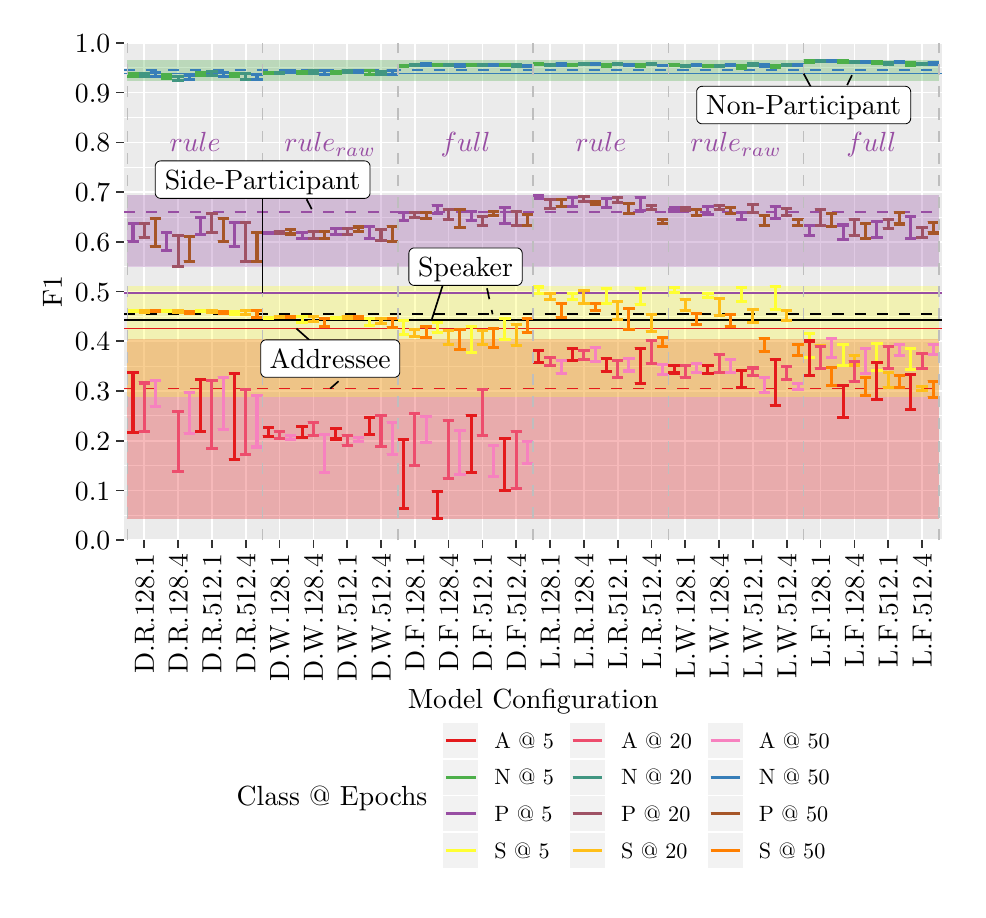
\begin{tikzpicture}[x=1pt,y=1pt]
\definecolor{fillColor}{RGB}{255,255,255}
\path[use as bounding box,fill=fillColor,fill opacity=0.00] (0,0) rectangle (336.00,311.47);
\begin{scope}
\path[clip] (  0.00,  0.00) rectangle (336.00,311.47);
\definecolor{drawColor}{RGB}{255,255,255}
\definecolor{fillColor}{RGB}{255,255,255}

\path[draw=drawColor,line width= 0.6pt,line join=round,line cap=round,fill=fillColor] (  0.00,  0.00) rectangle (336.00,311.47);
\end{scope}
\begin{scope}
\path[clip] ( 34.81,126.27) rectangle (330.50,305.97);
\definecolor{fillColor}{gray}{0.92}

\path[fill=fillColor] ( 34.81,126.27) rectangle (330.50,305.97);
\definecolor{drawColor}{RGB}{255,255,255}

\path[draw=drawColor,line width= 0.3pt,line join=round] ( 34.81,135.25) --
	(330.50,135.25);

\path[draw=drawColor,line width= 0.3pt,line join=round] ( 34.81,153.22) --
	(330.50,153.22);

\path[draw=drawColor,line width= 0.3pt,line join=round] ( 34.81,171.19) --
	(330.50,171.19);

\path[draw=drawColor,line width= 0.3pt,line join=round] ( 34.81,189.16) --
	(330.50,189.16);

\path[draw=drawColor,line width= 0.3pt,line join=round] ( 34.81,207.13) --
	(330.50,207.13);

\path[draw=drawColor,line width= 0.3pt,line join=round] ( 34.81,225.11) --
	(330.50,225.11);

\path[draw=drawColor,line width= 0.3pt,line join=round] ( 34.81,243.08) --
	(330.50,243.08);

\path[draw=drawColor,line width= 0.3pt,line join=round] ( 34.81,261.05) --
	(330.50,261.05);

\path[draw=drawColor,line width= 0.3pt,line join=round] ( 34.81,279.02) --
	(330.50,279.02);

\path[draw=drawColor,line width= 0.3pt,line join=round] ( 34.81,296.99) --
	(330.50,296.99);

\path[draw=drawColor,line width= 0.6pt,line join=round] ( 34.81,126.27) --
	(330.50,126.27);

\path[draw=drawColor,line width= 0.6pt,line join=round] ( 34.81,144.24) --
	(330.50,144.24);

\path[draw=drawColor,line width= 0.6pt,line join=round] ( 34.81,162.21) --
	(330.50,162.21);

\path[draw=drawColor,line width= 0.6pt,line join=round] ( 34.81,180.18) --
	(330.50,180.18);

\path[draw=drawColor,line width= 0.6pt,line join=round] ( 34.81,198.15) --
	(330.50,198.15);

\path[draw=drawColor,line width= 0.6pt,line join=round] ( 34.81,216.12) --
	(330.50,216.12);

\path[draw=drawColor,line width= 0.6pt,line join=round] ( 34.81,234.09) --
	(330.50,234.09);

\path[draw=drawColor,line width= 0.6pt,line join=round] ( 34.81,252.06) --
	(330.50,252.06);

\path[draw=drawColor,line width= 0.6pt,line join=round] ( 34.81,270.03) --
	(330.50,270.03);

\path[draw=drawColor,line width= 0.6pt,line join=round] ( 34.81,288.00) --
	(330.50,288.00);

\path[draw=drawColor,line width= 0.6pt,line join=round] ( 34.81,305.97) --
	(330.50,305.97);

\path[draw=drawColor,line width= 0.6pt,line join=round] ( 42.14,126.27) --
	( 42.14,305.97);

\path[draw=drawColor,line width= 0.6pt,line join=round] ( 54.36,126.27) --
	( 54.36,305.97);

\path[draw=drawColor,line width= 0.6pt,line join=round] ( 66.57,126.27) --
	( 66.57,305.97);

\path[draw=drawColor,line width= 0.6pt,line join=round] ( 78.79,126.27) --
	( 78.79,305.97);

\path[draw=drawColor,line width= 0.6pt,line join=round] ( 91.01,126.27) --
	( 91.01,305.97);

\path[draw=drawColor,line width= 0.6pt,line join=round] (103.23,126.27) --
	(103.23,305.97);

\path[draw=drawColor,line width= 0.6pt,line join=round] (115.45,126.27) --
	(115.45,305.97);

\path[draw=drawColor,line width= 0.6pt,line join=round] (127.67,126.27) --
	(127.67,305.97);

\path[draw=drawColor,line width= 0.6pt,line join=round] (139.89,126.27) --
	(139.89,305.97);

\path[draw=drawColor,line width= 0.6pt,line join=round] (152.11,126.27) --
	(152.11,305.97);

\path[draw=drawColor,line width= 0.6pt,line join=round] (164.32,126.27) --
	(164.32,305.97);

\path[draw=drawColor,line width= 0.6pt,line join=round] (176.54,126.27) --
	(176.54,305.97);

\path[draw=drawColor,line width= 0.6pt,line join=round] (188.76,126.27) --
	(188.76,305.97);

\path[draw=drawColor,line width= 0.6pt,line join=round] (200.98,126.27) --
	(200.98,305.97);

\path[draw=drawColor,line width= 0.6pt,line join=round] (213.20,126.27) --
	(213.20,305.97);

\path[draw=drawColor,line width= 0.6pt,line join=round] (225.42,126.27) --
	(225.42,305.97);

\path[draw=drawColor,line width= 0.6pt,line join=round] (237.64,126.27) --
	(237.64,305.97);

\path[draw=drawColor,line width= 0.6pt,line join=round] (249.86,126.27) --
	(249.86,305.97);

\path[draw=drawColor,line width= 0.6pt,line join=round] (262.07,126.27) --
	(262.07,305.97);

\path[draw=drawColor,line width= 0.6pt,line join=round] (274.29,126.27) --
	(274.29,305.97);

\path[draw=drawColor,line width= 0.6pt,line join=round] (286.51,126.27) --
	(286.51,305.97);

\path[draw=drawColor,line width= 0.6pt,line join=round] (298.73,126.27) --
	(298.73,305.97);

\path[draw=drawColor,line width= 0.6pt,line join=round] (310.95,126.27) --
	(310.95,305.97);

\path[draw=drawColor,line width= 0.6pt,line join=round] (323.17,126.27) --
	(323.17,305.97);
\definecolor{fillColor}{RGB}{228,26,28}

\path[fill=fillColor,fill opacity=0.30] ( 36.03,133.99) rectangle (329.28,199.12);
\definecolor{fillColor}{RGB}{255,255,51}

\path[fill=fillColor,fill opacity=0.30] ( 36.03,177.98) rectangle (329.28,218.05);
\definecolor{fillColor}{RGB}{152,78,163}

\path[fill=fillColor,fill opacity=0.30] ( 36.03,225.14) rectangle (329.28,250.99);
\definecolor{fillColor}{RGB}{77,175,74}

\path[fill=fillColor,fill opacity=0.30] ( 36.03,292.28) rectangle (329.28,299.61);
\definecolor{drawColor}{RGB}{0,0,0}

\path[draw=drawColor,line width= 0.6pt,line join=round] ( 34.81,205.91) -- (330.50,205.91);
\definecolor{drawColor}{RGB}{55,126,184}

\path[draw=drawColor,line width= 0.6pt,line join=round] ( 34.81,294.87) -- (330.50,294.87);
\definecolor{drawColor}{RGB}{228,26,28}

\path[draw=drawColor,line width= 0.6pt,line join=round] ( 34.81,202.74) -- (330.50,202.74);
\definecolor{drawColor}{RGB}{152,78,163}

\path[draw=drawColor,line width= 0.6pt,line join=round] ( 34.81,215.68) -- (330.50,215.68);
\definecolor{drawColor}{RGB}{0,0,0}

\path[draw=drawColor,line width= 0.6pt,dash pattern=on 4pt off 4pt ,line join=round] ( 34.81,207.89) -- (330.50,207.89);
\definecolor{drawColor}{RGB}{55,126,184}

\path[draw=drawColor,line width= 0.6pt,dash pattern=on 4pt off 4pt ,line join=round] ( 34.81,296.10) -- (330.50,296.10);
\definecolor{drawColor}{RGB}{228,26,28}

\path[draw=drawColor,line width= 0.6pt,dash pattern=on 4pt off 4pt ,line join=round] ( 34.81,181.05) -- (330.50,181.05);
\definecolor{drawColor}{RGB}{152,78,163}

\path[draw=drawColor,line width= 0.6pt,dash pattern=on 4pt off 4pt ,line join=round] ( 34.81,244.76) -- (330.50,244.76);
\definecolor{drawColor}{RGB}{255,127,0}

\path[draw=drawColor,line width= 1.1pt,line join=round] ( 44.17,209.27) --
	( 48.25,209.27);

\path[draw=drawColor,line width= 1.1pt,line join=round] ( 46.21,209.27) --
	( 46.21,208.75);

\path[draw=drawColor,line width= 1.1pt,line join=round] ( 44.17,208.75) --
	( 48.25,208.75);

\path[draw=drawColor,line width= 1.1pt,line join=round] ( 44.17,209.27) --
	( 48.25,209.27);

\path[draw=drawColor,line width= 1.1pt,line join=round] ( 46.21,209.27) --
	( 46.21,208.75);

\path[draw=drawColor,line width= 1.1pt,line join=round] ( 44.17,208.75) --
	( 48.25,208.75);

\path[draw=drawColor,line width= 1.1pt,line join=round] ( 44.17,209.27) --
	( 48.25,209.27);

\path[draw=drawColor,line width= 1.1pt,line join=round] ( 46.21,209.27) --
	( 46.21,208.75);

\path[draw=drawColor,line width= 1.1pt,line join=round] ( 44.17,208.75) --
	( 48.25,208.75);

\path[draw=drawColor,line width= 1.1pt,line join=round] ( 44.17,209.27) --
	( 48.25,209.27);

\path[draw=drawColor,line width= 1.1pt,line join=round] ( 46.21,209.27) --
	( 46.21,208.75);

\path[draw=drawColor,line width= 1.1pt,line join=round] ( 44.17,208.75) --
	( 48.25,208.75);

\path[draw=drawColor,line width= 1.1pt,line join=round] ( 44.17,209.27) --
	( 48.25,209.27);

\path[draw=drawColor,line width= 1.1pt,line join=round] ( 46.21,209.27) --
	( 46.21,208.75);

\path[draw=drawColor,line width= 1.1pt,line join=round] ( 44.17,208.75) --
	( 48.25,208.75);

\path[draw=drawColor,line width= 1.1pt,line join=round] ( 44.17,209.27) --
	( 48.25,209.27);

\path[draw=drawColor,line width= 1.1pt,line join=round] ( 46.21,209.27) --
	( 46.21,208.75);

\path[draw=drawColor,line width= 1.1pt,line join=round] ( 44.17,208.75) --
	( 48.25,208.75);

\path[draw=drawColor,line width= 1.1pt,line join=round] ( 44.17,209.27) --
	( 48.25,209.27);

\path[draw=drawColor,line width= 1.1pt,line join=round] ( 46.21,209.27) --
	( 46.21,208.75);

\path[draw=drawColor,line width= 1.1pt,line join=round] ( 44.17,208.75) --
	( 48.25,208.75);

\path[draw=drawColor,line width= 1.1pt,line join=round] ( 44.17,209.27) --
	( 48.25,209.27);

\path[draw=drawColor,line width= 1.1pt,line join=round] ( 46.21,209.27) --
	( 46.21,208.75);

\path[draw=drawColor,line width= 1.1pt,line join=round] ( 44.17,208.75) --
	( 48.25,208.75);
\definecolor{drawColor}{RGB}{255,191,25}

\path[draw=drawColor,line width= 1.1pt,line join=round] ( 40.10,209.16) --
	( 44.17,209.16);

\path[draw=drawColor,line width= 1.1pt,line join=round] ( 42.14,209.16) --
	( 42.14,208.71);

\path[draw=drawColor,line width= 1.1pt,line join=round] ( 40.10,208.71) --
	( 44.17,208.71);

\path[draw=drawColor,line width= 1.1pt,line join=round] ( 40.10,209.16) --
	( 44.17,209.16);

\path[draw=drawColor,line width= 1.1pt,line join=round] ( 42.14,209.16) --
	( 42.14,208.71);

\path[draw=drawColor,line width= 1.1pt,line join=round] ( 40.10,208.71) --
	( 44.17,208.71);

\path[draw=drawColor,line width= 1.1pt,line join=round] ( 40.10,209.16) --
	( 44.17,209.16);

\path[draw=drawColor,line width= 1.1pt,line join=round] ( 42.14,209.16) --
	( 42.14,208.71);

\path[draw=drawColor,line width= 1.1pt,line join=round] ( 40.10,208.71) --
	( 44.17,208.71);

\path[draw=drawColor,line width= 1.1pt,line join=round] ( 40.10,209.16) --
	( 44.17,209.16);

\path[draw=drawColor,line width= 1.1pt,line join=round] ( 42.14,209.16) --
	( 42.14,208.71);

\path[draw=drawColor,line width= 1.1pt,line join=round] ( 40.10,208.71) --
	( 44.17,208.71);

\path[draw=drawColor,line width= 1.1pt,line join=round] ( 40.10,209.16) --
	( 44.17,209.16);

\path[draw=drawColor,line width= 1.1pt,line join=round] ( 42.14,209.16) --
	( 42.14,208.71);

\path[draw=drawColor,line width= 1.1pt,line join=round] ( 40.10,208.71) --
	( 44.17,208.71);

\path[draw=drawColor,line width= 1.1pt,line join=round] ( 40.10,209.16) --
	( 44.17,209.16);

\path[draw=drawColor,line width= 1.1pt,line join=round] ( 42.14,209.16) --
	( 42.14,208.71);

\path[draw=drawColor,line width= 1.1pt,line join=round] ( 40.10,208.71) --
	( 44.17,208.71);

\path[draw=drawColor,line width= 1.1pt,line join=round] ( 40.10,209.16) --
	( 44.17,209.16);

\path[draw=drawColor,line width= 1.1pt,line join=round] ( 42.14,209.16) --
	( 42.14,208.71);

\path[draw=drawColor,line width= 1.1pt,line join=round] ( 40.10,208.71) --
	( 44.17,208.71);

\path[draw=drawColor,line width= 1.1pt,line join=round] ( 40.10,209.16) --
	( 44.17,209.16);

\path[draw=drawColor,line width= 1.1pt,line join=round] ( 42.14,209.16) --
	( 42.14,208.71);

\path[draw=drawColor,line width= 1.1pt,line join=round] ( 40.10,208.71) --
	( 44.17,208.71);
\definecolor{drawColor}{RGB}{255,255,51}

\path[draw=drawColor,line width= 1.1pt,line join=round] ( 36.03,209.30) --
	( 40.10,209.30);

\path[draw=drawColor,line width= 1.1pt,line join=round] ( 38.06,209.30) --
	( 38.06,209.08);

\path[draw=drawColor,line width= 1.1pt,line join=round] ( 36.03,209.08) --
	( 40.10,209.08);

\path[draw=drawColor,line width= 1.1pt,line join=round] ( 36.03,209.30) --
	( 40.10,209.30);

\path[draw=drawColor,line width= 1.1pt,line join=round] ( 38.06,209.30) --
	( 38.06,209.08);

\path[draw=drawColor,line width= 1.1pt,line join=round] ( 36.03,209.08) --
	( 40.10,209.08);

\path[draw=drawColor,line width= 1.1pt,line join=round] ( 36.03,209.30) --
	( 40.10,209.30);

\path[draw=drawColor,line width= 1.1pt,line join=round] ( 38.06,209.30) --
	( 38.06,209.08);

\path[draw=drawColor,line width= 1.1pt,line join=round] ( 36.03,209.08) --
	( 40.10,209.08);

\path[draw=drawColor,line width= 1.1pt,line join=round] ( 36.03,209.30) --
	( 40.10,209.30);

\path[draw=drawColor,line width= 1.1pt,line join=round] ( 38.06,209.30) --
	( 38.06,209.08);

\path[draw=drawColor,line width= 1.1pt,line join=round] ( 36.03,209.08) --
	( 40.10,209.08);

\path[draw=drawColor,line width= 1.1pt,line join=round] ( 36.03,209.30) --
	( 40.10,209.30);

\path[draw=drawColor,line width= 1.1pt,line join=round] ( 38.06,209.30) --
	( 38.06,209.08);

\path[draw=drawColor,line width= 1.1pt,line join=round] ( 36.03,209.08) --
	( 40.10,209.08);

\path[draw=drawColor,line width= 1.1pt,line join=round] ( 36.03,209.30) --
	( 40.10,209.30);

\path[draw=drawColor,line width= 1.1pt,line join=round] ( 38.06,209.30) --
	( 38.06,209.08);

\path[draw=drawColor,line width= 1.1pt,line join=round] ( 36.03,209.08) --
	( 40.10,209.08);

\path[draw=drawColor,line width= 1.1pt,line join=round] ( 36.03,209.30) --
	( 40.10,209.30);

\path[draw=drawColor,line width= 1.1pt,line join=round] ( 38.06,209.30) --
	( 38.06,209.08);

\path[draw=drawColor,line width= 1.1pt,line join=round] ( 36.03,209.08) --
	( 40.10,209.08);

\path[draw=drawColor,line width= 1.1pt,line join=round] ( 36.03,209.30) --
	( 40.10,209.30);

\path[draw=drawColor,line width= 1.1pt,line join=round] ( 38.06,209.30) --
	( 38.06,209.08);

\path[draw=drawColor,line width= 1.1pt,line join=round] ( 36.03,209.08) --
	( 40.10,209.08);
\definecolor{drawColor}{RGB}{255,127,0}

\path[draw=drawColor,line width= 1.1pt,line join=round] ( 56.39,209.06) --
	( 60.47,209.06);

\path[draw=drawColor,line width= 1.1pt,line join=round] ( 58.43,209.06) --
	( 58.43,208.12);

\path[draw=drawColor,line width= 1.1pt,line join=round] ( 56.39,208.12) --
	( 60.47,208.12);

\path[draw=drawColor,line width= 1.1pt,line join=round] ( 56.39,209.06) --
	( 60.47,209.06);

\path[draw=drawColor,line width= 1.1pt,line join=round] ( 58.43,209.06) --
	( 58.43,208.12);

\path[draw=drawColor,line width= 1.1pt,line join=round] ( 56.39,208.12) --
	( 60.47,208.12);

\path[draw=drawColor,line width= 1.1pt,line join=round] ( 56.39,209.06) --
	( 60.47,209.06);

\path[draw=drawColor,line width= 1.1pt,line join=round] ( 58.43,209.06) --
	( 58.43,208.12);

\path[draw=drawColor,line width= 1.1pt,line join=round] ( 56.39,208.12) --
	( 60.47,208.12);

\path[draw=drawColor,line width= 1.1pt,line join=round] ( 56.39,209.06) --
	( 60.47,209.06);

\path[draw=drawColor,line width= 1.1pt,line join=round] ( 58.43,209.06) --
	( 58.43,208.12);

\path[draw=drawColor,line width= 1.1pt,line join=round] ( 56.39,208.12) --
	( 60.47,208.12);

\path[draw=drawColor,line width= 1.1pt,line join=round] ( 56.39,209.06) --
	( 60.47,209.06);

\path[draw=drawColor,line width= 1.1pt,line join=round] ( 58.43,209.06) --
	( 58.43,208.12);

\path[draw=drawColor,line width= 1.1pt,line join=round] ( 56.39,208.12) --
	( 60.47,208.12);

\path[draw=drawColor,line width= 1.1pt,line join=round] ( 56.39,209.06) --
	( 60.47,209.06);

\path[draw=drawColor,line width= 1.1pt,line join=round] ( 58.43,209.06) --
	( 58.43,208.12);

\path[draw=drawColor,line width= 1.1pt,line join=round] ( 56.39,208.12) --
	( 60.47,208.12);

\path[draw=drawColor,line width= 1.1pt,line join=round] ( 56.39,209.06) --
	( 60.47,209.06);

\path[draw=drawColor,line width= 1.1pt,line join=round] ( 58.43,209.06) --
	( 58.43,208.12);

\path[draw=drawColor,line width= 1.1pt,line join=round] ( 56.39,208.12) --
	( 60.47,208.12);

\path[draw=drawColor,line width= 1.1pt,line join=round] ( 56.39,209.06) --
	( 60.47,209.06);

\path[draw=drawColor,line width= 1.1pt,line join=round] ( 58.43,209.06) --
	( 58.43,208.12);

\path[draw=drawColor,line width= 1.1pt,line join=round] ( 56.39,208.12) --
	( 60.47,208.12);
\definecolor{drawColor}{RGB}{255,191,25}

\path[draw=drawColor,line width= 1.1pt,line join=round] ( 52.32,209.22) --
	( 56.39,209.22);

\path[draw=drawColor,line width= 1.1pt,line join=round] ( 54.36,209.22) --
	( 54.36,208.48);

\path[draw=drawColor,line width= 1.1pt,line join=round] ( 52.32,208.48) --
	( 56.39,208.48);

\path[draw=drawColor,line width= 1.1pt,line join=round] ( 52.32,209.22) --
	( 56.39,209.22);

\path[draw=drawColor,line width= 1.1pt,line join=round] ( 54.36,209.22) --
	( 54.36,208.48);

\path[draw=drawColor,line width= 1.1pt,line join=round] ( 52.32,208.48) --
	( 56.39,208.48);

\path[draw=drawColor,line width= 1.1pt,line join=round] ( 52.32,209.22) --
	( 56.39,209.22);

\path[draw=drawColor,line width= 1.1pt,line join=round] ( 54.36,209.22) --
	( 54.36,208.48);

\path[draw=drawColor,line width= 1.1pt,line join=round] ( 52.32,208.48) --
	( 56.39,208.48);

\path[draw=drawColor,line width= 1.1pt,line join=round] ( 52.32,209.22) --
	( 56.39,209.22);

\path[draw=drawColor,line width= 1.1pt,line join=round] ( 54.36,209.22) --
	( 54.36,208.48);

\path[draw=drawColor,line width= 1.1pt,line join=round] ( 52.32,208.48) --
	( 56.39,208.48);

\path[draw=drawColor,line width= 1.1pt,line join=round] ( 52.32,209.22) --
	( 56.39,209.22);

\path[draw=drawColor,line width= 1.1pt,line join=round] ( 54.36,209.22) --
	( 54.36,208.48);

\path[draw=drawColor,line width= 1.1pt,line join=round] ( 52.32,208.48) --
	( 56.39,208.48);

\path[draw=drawColor,line width= 1.1pt,line join=round] ( 52.32,209.22) --
	( 56.39,209.22);

\path[draw=drawColor,line width= 1.1pt,line join=round] ( 54.36,209.22) --
	( 54.36,208.48);

\path[draw=drawColor,line width= 1.1pt,line join=round] ( 52.32,208.48) --
	( 56.39,208.48);

\path[draw=drawColor,line width= 1.1pt,line join=round] ( 52.32,209.22) --
	( 56.39,209.22);

\path[draw=drawColor,line width= 1.1pt,line join=round] ( 54.36,209.22) --
	( 54.36,208.48);

\path[draw=drawColor,line width= 1.1pt,line join=round] ( 52.32,208.48) --
	( 56.39,208.48);

\path[draw=drawColor,line width= 1.1pt,line join=round] ( 52.32,209.22) --
	( 56.39,209.22);

\path[draw=drawColor,line width= 1.1pt,line join=round] ( 54.36,209.22) --
	( 54.36,208.48);

\path[draw=drawColor,line width= 1.1pt,line join=round] ( 52.32,208.48) --
	( 56.39,208.48);
\definecolor{drawColor}{RGB}{255,255,51}

\path[draw=drawColor,line width= 1.1pt,line join=round] ( 48.25,209.26) --
	( 52.32,209.26);

\path[draw=drawColor,line width= 1.1pt,line join=round] ( 50.28,209.26) --
	( 50.28,208.78);

\path[draw=drawColor,line width= 1.1pt,line join=round] ( 48.25,208.78) --
	( 52.32,208.78);

\path[draw=drawColor,line width= 1.1pt,line join=round] ( 48.25,209.26) --
	( 52.32,209.26);

\path[draw=drawColor,line width= 1.1pt,line join=round] ( 50.28,209.26) --
	( 50.28,208.78);

\path[draw=drawColor,line width= 1.1pt,line join=round] ( 48.25,208.78) --
	( 52.32,208.78);

\path[draw=drawColor,line width= 1.1pt,line join=round] ( 48.25,209.26) --
	( 52.32,209.26);

\path[draw=drawColor,line width= 1.1pt,line join=round] ( 50.28,209.26) --
	( 50.28,208.78);

\path[draw=drawColor,line width= 1.1pt,line join=round] ( 48.25,208.78) --
	( 52.32,208.78);

\path[draw=drawColor,line width= 1.1pt,line join=round] ( 48.25,209.26) --
	( 52.32,209.26);

\path[draw=drawColor,line width= 1.1pt,line join=round] ( 50.28,209.26) --
	( 50.28,208.78);

\path[draw=drawColor,line width= 1.1pt,line join=round] ( 48.25,208.78) --
	( 52.32,208.78);

\path[draw=drawColor,line width= 1.1pt,line join=round] ( 48.25,209.26) --
	( 52.32,209.26);

\path[draw=drawColor,line width= 1.1pt,line join=round] ( 50.28,209.26) --
	( 50.28,208.78);

\path[draw=drawColor,line width= 1.1pt,line join=round] ( 48.25,208.78) --
	( 52.32,208.78);

\path[draw=drawColor,line width= 1.1pt,line join=round] ( 48.25,209.26) --
	( 52.32,209.26);

\path[draw=drawColor,line width= 1.1pt,line join=round] ( 50.28,209.26) --
	( 50.28,208.78);

\path[draw=drawColor,line width= 1.1pt,line join=round] ( 48.25,208.78) --
	( 52.32,208.78);

\path[draw=drawColor,line width= 1.1pt,line join=round] ( 48.25,209.26) --
	( 52.32,209.26);

\path[draw=drawColor,line width= 1.1pt,line join=round] ( 50.28,209.26) --
	( 50.28,208.78);

\path[draw=drawColor,line width= 1.1pt,line join=round] ( 48.25,208.78) --
	( 52.32,208.78);

\path[draw=drawColor,line width= 1.1pt,line join=round] ( 48.25,209.26) --
	( 52.32,209.26);

\path[draw=drawColor,line width= 1.1pt,line join=round] ( 50.28,209.26) --
	( 50.28,208.78);

\path[draw=drawColor,line width= 1.1pt,line join=round] ( 48.25,208.78) --
	( 52.32,208.78);
\definecolor{drawColor}{RGB}{255,127,0}

\path[draw=drawColor,line width= 1.1pt,line join=round] ( 68.61,209.01) --
	( 72.68,209.01);

\path[draw=drawColor,line width= 1.1pt,line join=round] ( 70.65,209.01) --
	( 70.65,208.34);

\path[draw=drawColor,line width= 1.1pt,line join=round] ( 68.61,208.34) --
	( 72.68,208.34);

\path[draw=drawColor,line width= 1.1pt,line join=round] ( 68.61,209.01) --
	( 72.68,209.01);

\path[draw=drawColor,line width= 1.1pt,line join=round] ( 70.65,209.01) --
	( 70.65,208.34);

\path[draw=drawColor,line width= 1.1pt,line join=round] ( 68.61,208.34) --
	( 72.68,208.34);

\path[draw=drawColor,line width= 1.1pt,line join=round] ( 68.61,209.01) --
	( 72.68,209.01);

\path[draw=drawColor,line width= 1.1pt,line join=round] ( 70.65,209.01) --
	( 70.65,208.34);

\path[draw=drawColor,line width= 1.1pt,line join=round] ( 68.61,208.34) --
	( 72.68,208.34);

\path[draw=drawColor,line width= 1.1pt,line join=round] ( 68.61,209.01) --
	( 72.68,209.01);

\path[draw=drawColor,line width= 1.1pt,line join=round] ( 70.65,209.01) --
	( 70.65,208.34);

\path[draw=drawColor,line width= 1.1pt,line join=round] ( 68.61,208.34) --
	( 72.68,208.34);

\path[draw=drawColor,line width= 1.1pt,line join=round] ( 68.61,209.01) --
	( 72.68,209.01);

\path[draw=drawColor,line width= 1.1pt,line join=round] ( 70.65,209.01) --
	( 70.65,208.34);

\path[draw=drawColor,line width= 1.1pt,line join=round] ( 68.61,208.34) --
	( 72.68,208.34);

\path[draw=drawColor,line width= 1.1pt,line join=round] ( 68.61,209.01) --
	( 72.68,209.01);

\path[draw=drawColor,line width= 1.1pt,line join=round] ( 70.65,209.01) --
	( 70.65,208.34);

\path[draw=drawColor,line width= 1.1pt,line join=round] ( 68.61,208.34) --
	( 72.68,208.34);

\path[draw=drawColor,line width= 1.1pt,line join=round] ( 68.61,209.01) --
	( 72.68,209.01);

\path[draw=drawColor,line width= 1.1pt,line join=round] ( 70.65,209.01) --
	( 70.65,208.34);

\path[draw=drawColor,line width= 1.1pt,line join=round] ( 68.61,208.34) --
	( 72.68,208.34);

\path[draw=drawColor,line width= 1.1pt,line join=round] ( 68.61,209.01) --
	( 72.68,209.01);

\path[draw=drawColor,line width= 1.1pt,line join=round] ( 70.65,209.01) --
	( 70.65,208.34);

\path[draw=drawColor,line width= 1.1pt,line join=round] ( 68.61,208.34) --
	( 72.68,208.34);
\definecolor{drawColor}{RGB}{255,191,25}

\path[draw=drawColor,line width= 1.1pt,line join=round] ( 64.54,209.08) --
	( 68.61,209.08);

\path[draw=drawColor,line width= 1.1pt,line join=round] ( 66.57,209.08) --
	( 66.57,208.41);

\path[draw=drawColor,line width= 1.1pt,line join=round] ( 64.54,208.41) --
	( 68.61,208.41);

\path[draw=drawColor,line width= 1.1pt,line join=round] ( 64.54,209.08) --
	( 68.61,209.08);

\path[draw=drawColor,line width= 1.1pt,line join=round] ( 66.57,209.08) --
	( 66.57,208.41);

\path[draw=drawColor,line width= 1.1pt,line join=round] ( 64.54,208.41) --
	( 68.61,208.41);

\path[draw=drawColor,line width= 1.1pt,line join=round] ( 64.54,209.08) --
	( 68.61,209.08);

\path[draw=drawColor,line width= 1.1pt,line join=round] ( 66.57,209.08) --
	( 66.57,208.41);

\path[draw=drawColor,line width= 1.1pt,line join=round] ( 64.54,208.41) --
	( 68.61,208.41);

\path[draw=drawColor,line width= 1.1pt,line join=round] ( 64.54,209.08) --
	( 68.61,209.08);

\path[draw=drawColor,line width= 1.1pt,line join=round] ( 66.57,209.08) --
	( 66.57,208.41);

\path[draw=drawColor,line width= 1.1pt,line join=round] ( 64.54,208.41) --
	( 68.61,208.41);

\path[draw=drawColor,line width= 1.1pt,line join=round] ( 64.54,209.08) --
	( 68.61,209.08);

\path[draw=drawColor,line width= 1.1pt,line join=round] ( 66.57,209.08) --
	( 66.57,208.41);

\path[draw=drawColor,line width= 1.1pt,line join=round] ( 64.54,208.41) --
	( 68.61,208.41);

\path[draw=drawColor,line width= 1.1pt,line join=round] ( 64.54,209.08) --
	( 68.61,209.08);

\path[draw=drawColor,line width= 1.1pt,line join=round] ( 66.57,209.08) --
	( 66.57,208.41);

\path[draw=drawColor,line width= 1.1pt,line join=round] ( 64.54,208.41) --
	( 68.61,208.41);

\path[draw=drawColor,line width= 1.1pt,line join=round] ( 64.54,209.08) --
	( 68.61,209.08);

\path[draw=drawColor,line width= 1.1pt,line join=round] ( 66.57,209.08) --
	( 66.57,208.41);

\path[draw=drawColor,line width= 1.1pt,line join=round] ( 64.54,208.41) --
	( 68.61,208.41);

\path[draw=drawColor,line width= 1.1pt,line join=round] ( 64.54,209.08) --
	( 68.61,209.08);

\path[draw=drawColor,line width= 1.1pt,line join=round] ( 66.57,209.08) --
	( 66.57,208.41);

\path[draw=drawColor,line width= 1.1pt,line join=round] ( 64.54,208.41) --
	( 68.61,208.41);
\definecolor{drawColor}{RGB}{255,255,51}

\path[draw=drawColor,line width= 1.1pt,line join=round] ( 60.47,209.15) --
	( 64.54,209.15);

\path[draw=drawColor,line width= 1.1pt,line join=round] ( 62.50,209.15) --
	( 62.50,208.89);

\path[draw=drawColor,line width= 1.1pt,line join=round] ( 60.47,208.89) --
	( 64.54,208.89);

\path[draw=drawColor,line width= 1.1pt,line join=round] ( 60.47,209.15) --
	( 64.54,209.15);

\path[draw=drawColor,line width= 1.1pt,line join=round] ( 62.50,209.15) --
	( 62.50,208.89);

\path[draw=drawColor,line width= 1.1pt,line join=round] ( 60.47,208.89) --
	( 64.54,208.89);

\path[draw=drawColor,line width= 1.1pt,line join=round] ( 60.47,209.15) --
	( 64.54,209.15);

\path[draw=drawColor,line width= 1.1pt,line join=round] ( 62.50,209.15) --
	( 62.50,208.89);

\path[draw=drawColor,line width= 1.1pt,line join=round] ( 60.47,208.89) --
	( 64.54,208.89);

\path[draw=drawColor,line width= 1.1pt,line join=round] ( 60.47,209.15) --
	( 64.54,209.15);

\path[draw=drawColor,line width= 1.1pt,line join=round] ( 62.50,209.15) --
	( 62.50,208.89);

\path[draw=drawColor,line width= 1.1pt,line join=round] ( 60.47,208.89) --
	( 64.54,208.89);

\path[draw=drawColor,line width= 1.1pt,line join=round] ( 60.47,209.15) --
	( 64.54,209.15);

\path[draw=drawColor,line width= 1.1pt,line join=round] ( 62.50,209.15) --
	( 62.50,208.89);

\path[draw=drawColor,line width= 1.1pt,line join=round] ( 60.47,208.89) --
	( 64.54,208.89);

\path[draw=drawColor,line width= 1.1pt,line join=round] ( 60.47,209.15) --
	( 64.54,209.15);

\path[draw=drawColor,line width= 1.1pt,line join=round] ( 62.50,209.15) --
	( 62.50,208.89);

\path[draw=drawColor,line width= 1.1pt,line join=round] ( 60.47,208.89) --
	( 64.54,208.89);

\path[draw=drawColor,line width= 1.1pt,line join=round] ( 60.47,209.15) --
	( 64.54,209.15);

\path[draw=drawColor,line width= 1.1pt,line join=round] ( 62.50,209.15) --
	( 62.50,208.89);

\path[draw=drawColor,line width= 1.1pt,line join=round] ( 60.47,208.89) --
	( 64.54,208.89);

\path[draw=drawColor,line width= 1.1pt,line join=round] ( 60.47,209.15) --
	( 64.54,209.15);

\path[draw=drawColor,line width= 1.1pt,line join=round] ( 62.50,209.15) --
	( 62.50,208.89);

\path[draw=drawColor,line width= 1.1pt,line join=round] ( 60.47,208.89) --
	( 64.54,208.89);
\definecolor{drawColor}{RGB}{255,127,0}

\path[draw=drawColor,line width= 1.1pt,line join=round] ( 80.83,209.30) --
	( 84.90,209.30);

\path[draw=drawColor,line width= 1.1pt,line join=round] ( 82.87,209.30) --
	( 82.87,206.63);

\path[draw=drawColor,line width= 1.1pt,line join=round] ( 80.83,206.63) --
	( 84.90,206.63);

\path[draw=drawColor,line width= 1.1pt,line join=round] ( 80.83,209.30) --
	( 84.90,209.30);

\path[draw=drawColor,line width= 1.1pt,line join=round] ( 82.87,209.30) --
	( 82.87,206.63);

\path[draw=drawColor,line width= 1.1pt,line join=round] ( 80.83,206.63) --
	( 84.90,206.63);

\path[draw=drawColor,line width= 1.1pt,line join=round] ( 80.83,209.30) --
	( 84.90,209.30);

\path[draw=drawColor,line width= 1.1pt,line join=round] ( 82.87,209.30) --
	( 82.87,206.63);

\path[draw=drawColor,line width= 1.1pt,line join=round] ( 80.83,206.63) --
	( 84.90,206.63);

\path[draw=drawColor,line width= 1.1pt,line join=round] ( 80.83,209.30) --
	( 84.90,209.30);

\path[draw=drawColor,line width= 1.1pt,line join=round] ( 82.87,209.30) --
	( 82.87,206.63);

\path[draw=drawColor,line width= 1.1pt,line join=round] ( 80.83,206.63) --
	( 84.90,206.63);

\path[draw=drawColor,line width= 1.1pt,line join=round] ( 80.83,209.30) --
	( 84.90,209.30);

\path[draw=drawColor,line width= 1.1pt,line join=round] ( 82.87,209.30) --
	( 82.87,206.63);

\path[draw=drawColor,line width= 1.1pt,line join=round] ( 80.83,206.63) --
	( 84.90,206.63);

\path[draw=drawColor,line width= 1.1pt,line join=round] ( 80.83,209.30) --
	( 84.90,209.30);

\path[draw=drawColor,line width= 1.1pt,line join=round] ( 82.87,209.30) --
	( 82.87,206.63);

\path[draw=drawColor,line width= 1.1pt,line join=round] ( 80.83,206.63) --
	( 84.90,206.63);

\path[draw=drawColor,line width= 1.1pt,line join=round] ( 80.83,209.30) --
	( 84.90,209.30);

\path[draw=drawColor,line width= 1.1pt,line join=round] ( 82.87,209.30) --
	( 82.87,206.63);

\path[draw=drawColor,line width= 1.1pt,line join=round] ( 80.83,206.63) --
	( 84.90,206.63);

\path[draw=drawColor,line width= 1.1pt,line join=round] ( 80.83,209.30) --
	( 84.90,209.30);

\path[draw=drawColor,line width= 1.1pt,line join=round] ( 82.87,209.30) --
	( 82.87,206.63);

\path[draw=drawColor,line width= 1.1pt,line join=round] ( 80.83,206.63) --
	( 84.90,206.63);
\definecolor{drawColor}{RGB}{255,191,25}

\path[draw=drawColor,line width= 1.1pt,line join=round] ( 76.76,209.12) --
	( 80.83,209.12);

\path[draw=drawColor,line width= 1.1pt,line join=round] ( 78.79,209.12) --
	( 78.79,207.88);

\path[draw=drawColor,line width= 1.1pt,line join=round] ( 76.76,207.88) --
	( 80.83,207.88);

\path[draw=drawColor,line width= 1.1pt,line join=round] ( 76.76,209.12) --
	( 80.83,209.12);

\path[draw=drawColor,line width= 1.1pt,line join=round] ( 78.79,209.12) --
	( 78.79,207.88);

\path[draw=drawColor,line width= 1.1pt,line join=round] ( 76.76,207.88) --
	( 80.83,207.88);

\path[draw=drawColor,line width= 1.1pt,line join=round] ( 76.76,209.12) --
	( 80.83,209.12);

\path[draw=drawColor,line width= 1.1pt,line join=round] ( 78.79,209.12) --
	( 78.79,207.88);

\path[draw=drawColor,line width= 1.1pt,line join=round] ( 76.76,207.88) --
	( 80.83,207.88);

\path[draw=drawColor,line width= 1.1pt,line join=round] ( 76.76,209.12) --
	( 80.83,209.12);

\path[draw=drawColor,line width= 1.1pt,line join=round] ( 78.79,209.12) --
	( 78.79,207.88);

\path[draw=drawColor,line width= 1.1pt,line join=round] ( 76.76,207.88) --
	( 80.83,207.88);

\path[draw=drawColor,line width= 1.1pt,line join=round] ( 76.76,209.12) --
	( 80.83,209.12);

\path[draw=drawColor,line width= 1.1pt,line join=round] ( 78.79,209.12) --
	( 78.79,207.88);

\path[draw=drawColor,line width= 1.1pt,line join=round] ( 76.76,207.88) --
	( 80.83,207.88);

\path[draw=drawColor,line width= 1.1pt,line join=round] ( 76.76,209.12) --
	( 80.83,209.12);

\path[draw=drawColor,line width= 1.1pt,line join=round] ( 78.79,209.12) --
	( 78.79,207.88);

\path[draw=drawColor,line width= 1.1pt,line join=round] ( 76.76,207.88) --
	( 80.83,207.88);

\path[draw=drawColor,line width= 1.1pt,line join=round] ( 76.76,209.12) --
	( 80.83,209.12);

\path[draw=drawColor,line width= 1.1pt,line join=round] ( 78.79,209.12) --
	( 78.79,207.88);

\path[draw=drawColor,line width= 1.1pt,line join=round] ( 76.76,207.88) --
	( 80.83,207.88);

\path[draw=drawColor,line width= 1.1pt,line join=round] ( 76.76,209.12) --
	( 80.83,209.12);

\path[draw=drawColor,line width= 1.1pt,line join=round] ( 78.79,209.12) --
	( 78.79,207.88);

\path[draw=drawColor,line width= 1.1pt,line join=round] ( 76.76,207.88) --
	( 80.83,207.88);
\definecolor{drawColor}{RGB}{255,255,51}

\path[draw=drawColor,line width= 1.1pt,line join=round] ( 72.68,208.92) --
	( 76.76,208.92);

\path[draw=drawColor,line width= 1.1pt,line join=round] ( 74.72,208.92) --
	( 74.72,207.83);

\path[draw=drawColor,line width= 1.1pt,line join=round] ( 72.68,207.83) --
	( 76.76,207.83);

\path[draw=drawColor,line width= 1.1pt,line join=round] ( 72.68,208.92) --
	( 76.76,208.92);

\path[draw=drawColor,line width= 1.1pt,line join=round] ( 74.72,208.92) --
	( 74.72,207.83);

\path[draw=drawColor,line width= 1.1pt,line join=round] ( 72.68,207.83) --
	( 76.76,207.83);

\path[draw=drawColor,line width= 1.1pt,line join=round] ( 72.68,208.92) --
	( 76.76,208.92);

\path[draw=drawColor,line width= 1.1pt,line join=round] ( 74.72,208.92) --
	( 74.72,207.83);

\path[draw=drawColor,line width= 1.1pt,line join=round] ( 72.68,207.83) --
	( 76.76,207.83);

\path[draw=drawColor,line width= 1.1pt,line join=round] ( 72.68,208.92) --
	( 76.76,208.92);

\path[draw=drawColor,line width= 1.1pt,line join=round] ( 74.72,208.92) --
	( 74.72,207.83);

\path[draw=drawColor,line width= 1.1pt,line join=round] ( 72.68,207.83) --
	( 76.76,207.83);

\path[draw=drawColor,line width= 1.1pt,line join=round] ( 72.68,208.92) --
	( 76.76,208.92);

\path[draw=drawColor,line width= 1.1pt,line join=round] ( 74.72,208.92) --
	( 74.72,207.83);

\path[draw=drawColor,line width= 1.1pt,line join=round] ( 72.68,207.83) --
	( 76.76,207.83);

\path[draw=drawColor,line width= 1.1pt,line join=round] ( 72.68,208.92) --
	( 76.76,208.92);

\path[draw=drawColor,line width= 1.1pt,line join=round] ( 74.72,208.92) --
	( 74.72,207.83);

\path[draw=drawColor,line width= 1.1pt,line join=round] ( 72.68,207.83) --
	( 76.76,207.83);

\path[draw=drawColor,line width= 1.1pt,line join=round] ( 72.68,208.92) --
	( 76.76,208.92);

\path[draw=drawColor,line width= 1.1pt,line join=round] ( 74.72,208.92) --
	( 74.72,207.83);

\path[draw=drawColor,line width= 1.1pt,line join=round] ( 72.68,207.83) --
	( 76.76,207.83);

\path[draw=drawColor,line width= 1.1pt,line join=round] ( 72.68,208.92) --
	( 76.76,208.92);

\path[draw=drawColor,line width= 1.1pt,line join=round] ( 74.72,208.92) --
	( 74.72,207.83);

\path[draw=drawColor,line width= 1.1pt,line join=round] ( 72.68,207.83) --
	( 76.76,207.83);
\definecolor{drawColor}{RGB}{255,127,0}

\path[draw=drawColor,line width= 1.1pt,line join=round] ( 93.05,207.05) --
	( 97.12,207.05);

\path[draw=drawColor,line width= 1.1pt,line join=round] ( 95.09,207.05) --
	( 95.09,206.64);

\path[draw=drawColor,line width= 1.1pt,line join=round] ( 93.05,206.64) --
	( 97.12,206.64);

\path[draw=drawColor,line width= 1.1pt,line join=round] ( 93.05,207.05) --
	( 97.12,207.05);

\path[draw=drawColor,line width= 1.1pt,line join=round] ( 95.09,207.05) --
	( 95.09,206.64);

\path[draw=drawColor,line width= 1.1pt,line join=round] ( 93.05,206.64) --
	( 97.12,206.64);

\path[draw=drawColor,line width= 1.1pt,line join=round] ( 93.05,207.05) --
	( 97.12,207.05);

\path[draw=drawColor,line width= 1.1pt,line join=round] ( 95.09,207.05) --
	( 95.09,206.64);

\path[draw=drawColor,line width= 1.1pt,line join=round] ( 93.05,206.64) --
	( 97.12,206.64);

\path[draw=drawColor,line width= 1.1pt,line join=round] ( 93.05,207.05) --
	( 97.12,207.05);

\path[draw=drawColor,line width= 1.1pt,line join=round] ( 95.09,207.05) --
	( 95.09,206.64);

\path[draw=drawColor,line width= 1.1pt,line join=round] ( 93.05,206.64) --
	( 97.12,206.64);

\path[draw=drawColor,line width= 1.1pt,line join=round] ( 93.05,207.05) --
	( 97.12,207.05);

\path[draw=drawColor,line width= 1.1pt,line join=round] ( 95.09,207.05) --
	( 95.09,206.64);

\path[draw=drawColor,line width= 1.1pt,line join=round] ( 93.05,206.64) --
	( 97.12,206.64);

\path[draw=drawColor,line width= 1.1pt,line join=round] ( 93.05,207.05) --
	( 97.12,207.05);

\path[draw=drawColor,line width= 1.1pt,line join=round] ( 95.09,207.05) --
	( 95.09,206.64);

\path[draw=drawColor,line width= 1.1pt,line join=round] ( 93.05,206.64) --
	( 97.12,206.64);

\path[draw=drawColor,line width= 1.1pt,line join=round] ( 93.05,207.05) --
	( 97.12,207.05);

\path[draw=drawColor,line width= 1.1pt,line join=round] ( 95.09,207.05) --
	( 95.09,206.64);

\path[draw=drawColor,line width= 1.1pt,line join=round] ( 93.05,206.64) --
	( 97.12,206.64);

\path[draw=drawColor,line width= 1.1pt,line join=round] ( 93.05,207.05) --
	( 97.12,207.05);

\path[draw=drawColor,line width= 1.1pt,line join=round] ( 95.09,207.05) --
	( 95.09,206.64);

\path[draw=drawColor,line width= 1.1pt,line join=round] ( 93.05,206.64) --
	( 97.12,206.64);
\definecolor{drawColor}{RGB}{255,191,25}

\path[draw=drawColor,line width= 1.1pt,line join=round] ( 88.98,206.97) --
	( 93.05,206.97);

\path[draw=drawColor,line width= 1.1pt,line join=round] ( 91.01,206.97) --
	( 91.01,206.58);

\path[draw=drawColor,line width= 1.1pt,line join=round] ( 88.98,206.58) --
	( 93.05,206.58);

\path[draw=drawColor,line width= 1.1pt,line join=round] ( 88.98,206.97) --
	( 93.05,206.97);

\path[draw=drawColor,line width= 1.1pt,line join=round] ( 91.01,206.97) --
	( 91.01,206.58);

\path[draw=drawColor,line width= 1.1pt,line join=round] ( 88.98,206.58) --
	( 93.05,206.58);

\path[draw=drawColor,line width= 1.1pt,line join=round] ( 88.98,206.97) --
	( 93.05,206.97);

\path[draw=drawColor,line width= 1.1pt,line join=round] ( 91.01,206.97) --
	( 91.01,206.58);

\path[draw=drawColor,line width= 1.1pt,line join=round] ( 88.98,206.58) --
	( 93.05,206.58);

\path[draw=drawColor,line width= 1.1pt,line join=round] ( 88.98,206.97) --
	( 93.05,206.97);

\path[draw=drawColor,line width= 1.1pt,line join=round] ( 91.01,206.97) --
	( 91.01,206.58);

\path[draw=drawColor,line width= 1.1pt,line join=round] ( 88.98,206.58) --
	( 93.05,206.58);

\path[draw=drawColor,line width= 1.1pt,line join=round] ( 88.98,206.97) --
	( 93.05,206.97);

\path[draw=drawColor,line width= 1.1pt,line join=round] ( 91.01,206.97) --
	( 91.01,206.58);

\path[draw=drawColor,line width= 1.1pt,line join=round] ( 88.98,206.58) --
	( 93.05,206.58);

\path[draw=drawColor,line width= 1.1pt,line join=round] ( 88.98,206.97) --
	( 93.05,206.97);

\path[draw=drawColor,line width= 1.1pt,line join=round] ( 91.01,206.97) --
	( 91.01,206.58);

\path[draw=drawColor,line width= 1.1pt,line join=round] ( 88.98,206.58) --
	( 93.05,206.58);

\path[draw=drawColor,line width= 1.1pt,line join=round] ( 88.98,206.97) --
	( 93.05,206.97);

\path[draw=drawColor,line width= 1.1pt,line join=round] ( 91.01,206.97) --
	( 91.01,206.58);

\path[draw=drawColor,line width= 1.1pt,line join=round] ( 88.98,206.58) --
	( 93.05,206.58);

\path[draw=drawColor,line width= 1.1pt,line join=round] ( 88.98,206.97) --
	( 93.05,206.97);

\path[draw=drawColor,line width= 1.1pt,line join=round] ( 91.01,206.97) --
	( 91.01,206.58);

\path[draw=drawColor,line width= 1.1pt,line join=round] ( 88.98,206.58) --
	( 93.05,206.58);
\definecolor{drawColor}{RGB}{255,255,51}

\path[draw=drawColor,line width= 1.1pt,line join=round] ( 84.90,206.67) --
	( 88.98,206.67);

\path[draw=drawColor,line width= 1.1pt,line join=round] ( 86.94,206.67) --
	( 86.94,206.46);

\path[draw=drawColor,line width= 1.1pt,line join=round] ( 84.90,206.46) --
	( 88.98,206.46);

\path[draw=drawColor,line width= 1.1pt,line join=round] ( 84.90,206.67) --
	( 88.98,206.67);

\path[draw=drawColor,line width= 1.1pt,line join=round] ( 86.94,206.67) --
	( 86.94,206.46);

\path[draw=drawColor,line width= 1.1pt,line join=round] ( 84.90,206.46) --
	( 88.98,206.46);

\path[draw=drawColor,line width= 1.1pt,line join=round] ( 84.90,206.67) --
	( 88.98,206.67);

\path[draw=drawColor,line width= 1.1pt,line join=round] ( 86.94,206.67) --
	( 86.94,206.46);

\path[draw=drawColor,line width= 1.1pt,line join=round] ( 84.90,206.46) --
	( 88.98,206.46);

\path[draw=drawColor,line width= 1.1pt,line join=round] ( 84.90,206.67) --
	( 88.98,206.67);

\path[draw=drawColor,line width= 1.1pt,line join=round] ( 86.94,206.67) --
	( 86.94,206.46);

\path[draw=drawColor,line width= 1.1pt,line join=round] ( 84.90,206.46) --
	( 88.98,206.46);

\path[draw=drawColor,line width= 1.1pt,line join=round] ( 84.90,206.67) --
	( 88.98,206.67);

\path[draw=drawColor,line width= 1.1pt,line join=round] ( 86.94,206.67) --
	( 86.94,206.46);

\path[draw=drawColor,line width= 1.1pt,line join=round] ( 84.90,206.46) --
	( 88.98,206.46);

\path[draw=drawColor,line width= 1.1pt,line join=round] ( 84.90,206.67) --
	( 88.98,206.67);

\path[draw=drawColor,line width= 1.1pt,line join=round] ( 86.94,206.67) --
	( 86.94,206.46);

\path[draw=drawColor,line width= 1.1pt,line join=round] ( 84.90,206.46) --
	( 88.98,206.46);

\path[draw=drawColor,line width= 1.1pt,line join=round] ( 84.90,206.67) --
	( 88.98,206.67);

\path[draw=drawColor,line width= 1.1pt,line join=round] ( 86.94,206.67) --
	( 86.94,206.46);

\path[draw=drawColor,line width= 1.1pt,line join=round] ( 84.90,206.46) --
	( 88.98,206.46);

\path[draw=drawColor,line width= 1.1pt,line join=round] ( 84.90,206.67) --
	( 88.98,206.67);

\path[draw=drawColor,line width= 1.1pt,line join=round] ( 86.94,206.67) --
	( 86.94,206.46);

\path[draw=drawColor,line width= 1.1pt,line join=round] ( 84.90,206.46) --
	( 88.98,206.46);
\definecolor{drawColor}{RGB}{255,127,0}

\path[draw=drawColor,line width= 1.1pt,line join=round] (105.27,206.50) --
	(109.34,206.50);

\path[draw=drawColor,line width= 1.1pt,line join=round] (107.30,206.50) --
	(107.30,203.35);

\path[draw=drawColor,line width= 1.1pt,line join=round] (105.27,203.35) --
	(109.34,203.35);

\path[draw=drawColor,line width= 1.1pt,line join=round] (105.27,206.50) --
	(109.34,206.50);

\path[draw=drawColor,line width= 1.1pt,line join=round] (107.30,206.50) --
	(107.30,203.35);

\path[draw=drawColor,line width= 1.1pt,line join=round] (105.27,203.35) --
	(109.34,203.35);

\path[draw=drawColor,line width= 1.1pt,line join=round] (105.27,206.50) --
	(109.34,206.50);

\path[draw=drawColor,line width= 1.1pt,line join=round] (107.30,206.50) --
	(107.30,203.35);

\path[draw=drawColor,line width= 1.1pt,line join=round] (105.27,203.35) --
	(109.34,203.35);

\path[draw=drawColor,line width= 1.1pt,line join=round] (105.27,206.50) --
	(109.34,206.50);

\path[draw=drawColor,line width= 1.1pt,line join=round] (107.30,206.50) --
	(107.30,203.35);

\path[draw=drawColor,line width= 1.1pt,line join=round] (105.27,203.35) --
	(109.34,203.35);

\path[draw=drawColor,line width= 1.1pt,line join=round] (105.27,206.50) --
	(109.34,206.50);

\path[draw=drawColor,line width= 1.1pt,line join=round] (107.30,206.50) --
	(107.30,203.35);

\path[draw=drawColor,line width= 1.1pt,line join=round] (105.27,203.35) --
	(109.34,203.35);

\path[draw=drawColor,line width= 1.1pt,line join=round] (105.27,206.50) --
	(109.34,206.50);

\path[draw=drawColor,line width= 1.1pt,line join=round] (107.30,206.50) --
	(107.30,203.35);

\path[draw=drawColor,line width= 1.1pt,line join=round] (105.27,203.35) --
	(109.34,203.35);

\path[draw=drawColor,line width= 1.1pt,line join=round] (105.27,206.50) --
	(109.34,206.50);

\path[draw=drawColor,line width= 1.1pt,line join=round] (107.30,206.50) --
	(107.30,203.35);

\path[draw=drawColor,line width= 1.1pt,line join=round] (105.27,203.35) --
	(109.34,203.35);

\path[draw=drawColor,line width= 1.1pt,line join=round] (105.27,206.50) --
	(109.34,206.50);

\path[draw=drawColor,line width= 1.1pt,line join=round] (107.30,206.50) --
	(107.30,203.35);

\path[draw=drawColor,line width= 1.1pt,line join=round] (105.27,203.35) --
	(109.34,203.35);
\definecolor{drawColor}{RGB}{255,191,25}

\path[draw=drawColor,line width= 1.1pt,line join=round] (101.19,206.94) --
	(105.27,206.94);

\path[draw=drawColor,line width= 1.1pt,line join=round] (103.23,206.94) --
	(103.23,205.18);

\path[draw=drawColor,line width= 1.1pt,line join=round] (101.19,205.18) --
	(105.27,205.18);

\path[draw=drawColor,line width= 1.1pt,line join=round] (101.19,206.94) --
	(105.27,206.94);

\path[draw=drawColor,line width= 1.1pt,line join=round] (103.23,206.94) --
	(103.23,205.18);

\path[draw=drawColor,line width= 1.1pt,line join=round] (101.19,205.18) --
	(105.27,205.18);

\path[draw=drawColor,line width= 1.1pt,line join=round] (101.19,206.94) --
	(105.27,206.94);

\path[draw=drawColor,line width= 1.1pt,line join=round] (103.23,206.94) --
	(103.23,205.18);

\path[draw=drawColor,line width= 1.1pt,line join=round] (101.19,205.18) --
	(105.27,205.18);

\path[draw=drawColor,line width= 1.1pt,line join=round] (101.19,206.94) --
	(105.27,206.94);

\path[draw=drawColor,line width= 1.1pt,line join=round] (103.23,206.94) --
	(103.23,205.18);

\path[draw=drawColor,line width= 1.1pt,line join=round] (101.19,205.18) --
	(105.27,205.18);

\path[draw=drawColor,line width= 1.1pt,line join=round] (101.19,206.94) --
	(105.27,206.94);

\path[draw=drawColor,line width= 1.1pt,line join=round] (103.23,206.94) --
	(103.23,205.18);

\path[draw=drawColor,line width= 1.1pt,line join=round] (101.19,205.18) --
	(105.27,205.18);

\path[draw=drawColor,line width= 1.1pt,line join=round] (101.19,206.94) --
	(105.27,206.94);

\path[draw=drawColor,line width= 1.1pt,line join=round] (103.23,206.94) --
	(103.23,205.18);

\path[draw=drawColor,line width= 1.1pt,line join=round] (101.19,205.18) --
	(105.27,205.18);

\path[draw=drawColor,line width= 1.1pt,line join=round] (101.19,206.94) --
	(105.27,206.94);

\path[draw=drawColor,line width= 1.1pt,line join=round] (103.23,206.94) --
	(103.23,205.18);

\path[draw=drawColor,line width= 1.1pt,line join=round] (101.19,205.18) --
	(105.27,205.18);

\path[draw=drawColor,line width= 1.1pt,line join=round] (101.19,206.94) --
	(105.27,206.94);

\path[draw=drawColor,line width= 1.1pt,line join=round] (103.23,206.94) --
	(103.23,205.18);

\path[draw=drawColor,line width= 1.1pt,line join=round] (101.19,205.18) --
	(105.27,205.18);
\definecolor{drawColor}{RGB}{255,255,51}

\path[draw=drawColor,line width= 1.1pt,line join=round] ( 97.12,207.04) --
	(101.19,207.04);

\path[draw=drawColor,line width= 1.1pt,line join=round] ( 99.16,207.04) --
	( 99.16,204.83);

\path[draw=drawColor,line width= 1.1pt,line join=round] ( 97.12,204.83) --
	(101.19,204.83);

\path[draw=drawColor,line width= 1.1pt,line join=round] ( 97.12,207.04) --
	(101.19,207.04);

\path[draw=drawColor,line width= 1.1pt,line join=round] ( 99.16,207.04) --
	( 99.16,204.83);

\path[draw=drawColor,line width= 1.1pt,line join=round] ( 97.12,204.83) --
	(101.19,204.83);

\path[draw=drawColor,line width= 1.1pt,line join=round] ( 97.12,207.04) --
	(101.19,207.04);

\path[draw=drawColor,line width= 1.1pt,line join=round] ( 99.16,207.04) --
	( 99.16,204.83);

\path[draw=drawColor,line width= 1.1pt,line join=round] ( 97.12,204.83) --
	(101.19,204.83);

\path[draw=drawColor,line width= 1.1pt,line join=round] ( 97.12,207.04) --
	(101.19,207.04);

\path[draw=drawColor,line width= 1.1pt,line join=round] ( 99.16,207.04) --
	( 99.16,204.83);

\path[draw=drawColor,line width= 1.1pt,line join=round] ( 97.12,204.83) --
	(101.19,204.83);

\path[draw=drawColor,line width= 1.1pt,line join=round] ( 97.12,207.04) --
	(101.19,207.04);

\path[draw=drawColor,line width= 1.1pt,line join=round] ( 99.16,207.04) --
	( 99.16,204.83);

\path[draw=drawColor,line width= 1.1pt,line join=round] ( 97.12,204.83) --
	(101.19,204.83);

\path[draw=drawColor,line width= 1.1pt,line join=round] ( 97.12,207.04) --
	(101.19,207.04);

\path[draw=drawColor,line width= 1.1pt,line join=round] ( 99.16,207.04) --
	( 99.16,204.83);

\path[draw=drawColor,line width= 1.1pt,line join=round] ( 97.12,204.83) --
	(101.19,204.83);

\path[draw=drawColor,line width= 1.1pt,line join=round] ( 97.12,207.04) --
	(101.19,207.04);

\path[draw=drawColor,line width= 1.1pt,line join=round] ( 99.16,207.04) --
	( 99.16,204.83);

\path[draw=drawColor,line width= 1.1pt,line join=round] ( 97.12,204.83) --
	(101.19,204.83);

\path[draw=drawColor,line width= 1.1pt,line join=round] ( 97.12,207.04) --
	(101.19,207.04);

\path[draw=drawColor,line width= 1.1pt,line join=round] ( 99.16,207.04) --
	( 99.16,204.83);

\path[draw=drawColor,line width= 1.1pt,line join=round] ( 97.12,204.83) --
	(101.19,204.83);
\definecolor{drawColor}{RGB}{255,127,0}

\path[draw=drawColor,line width= 1.1pt,line join=round] (117.49,207.03) --
	(121.56,207.03);

\path[draw=drawColor,line width= 1.1pt,line join=round] (119.52,207.03) --
	(119.52,206.50);

\path[draw=drawColor,line width= 1.1pt,line join=round] (117.49,206.50) --
	(121.56,206.50);

\path[draw=drawColor,line width= 1.1pt,line join=round] (117.49,207.03) --
	(121.56,207.03);

\path[draw=drawColor,line width= 1.1pt,line join=round] (119.52,207.03) --
	(119.52,206.50);

\path[draw=drawColor,line width= 1.1pt,line join=round] (117.49,206.50) --
	(121.56,206.50);

\path[draw=drawColor,line width= 1.1pt,line join=round] (117.49,207.03) --
	(121.56,207.03);

\path[draw=drawColor,line width= 1.1pt,line join=round] (119.52,207.03) --
	(119.52,206.50);

\path[draw=drawColor,line width= 1.1pt,line join=round] (117.49,206.50) --
	(121.56,206.50);

\path[draw=drawColor,line width= 1.1pt,line join=round] (117.49,207.03) --
	(121.56,207.03);

\path[draw=drawColor,line width= 1.1pt,line join=round] (119.52,207.03) --
	(119.52,206.50);

\path[draw=drawColor,line width= 1.1pt,line join=round] (117.49,206.50) --
	(121.56,206.50);

\path[draw=drawColor,line width= 1.1pt,line join=round] (117.49,207.03) --
	(121.56,207.03);

\path[draw=drawColor,line width= 1.1pt,line join=round] (119.52,207.03) --
	(119.52,206.50);

\path[draw=drawColor,line width= 1.1pt,line join=round] (117.49,206.50) --
	(121.56,206.50);

\path[draw=drawColor,line width= 1.1pt,line join=round] (117.49,207.03) --
	(121.56,207.03);

\path[draw=drawColor,line width= 1.1pt,line join=round] (119.52,207.03) --
	(119.52,206.50);

\path[draw=drawColor,line width= 1.1pt,line join=round] (117.49,206.50) --
	(121.56,206.50);

\path[draw=drawColor,line width= 1.1pt,line join=round] (117.49,207.03) --
	(121.56,207.03);

\path[draw=drawColor,line width= 1.1pt,line join=round] (119.52,207.03) --
	(119.52,206.50);

\path[draw=drawColor,line width= 1.1pt,line join=round] (117.49,206.50) --
	(121.56,206.50);

\path[draw=drawColor,line width= 1.1pt,line join=round] (117.49,207.03) --
	(121.56,207.03);

\path[draw=drawColor,line width= 1.1pt,line join=round] (119.52,207.03) --
	(119.52,206.50);

\path[draw=drawColor,line width= 1.1pt,line join=round] (117.49,206.50) --
	(121.56,206.50);
\definecolor{drawColor}{RGB}{255,191,25}

\path[draw=drawColor,line width= 1.1pt,line join=round] (113.41,207.11) --
	(117.49,207.11);

\path[draw=drawColor,line width= 1.1pt,line join=round] (115.45,207.11) --
	(115.45,206.26);

\path[draw=drawColor,line width= 1.1pt,line join=round] (113.41,206.26) --
	(117.49,206.26);

\path[draw=drawColor,line width= 1.1pt,line join=round] (113.41,207.11) --
	(117.49,207.11);

\path[draw=drawColor,line width= 1.1pt,line join=round] (115.45,207.11) --
	(115.45,206.26);

\path[draw=drawColor,line width= 1.1pt,line join=round] (113.41,206.26) --
	(117.49,206.26);

\path[draw=drawColor,line width= 1.1pt,line join=round] (113.41,207.11) --
	(117.49,207.11);

\path[draw=drawColor,line width= 1.1pt,line join=round] (115.45,207.11) --
	(115.45,206.26);

\path[draw=drawColor,line width= 1.1pt,line join=round] (113.41,206.26) --
	(117.49,206.26);

\path[draw=drawColor,line width= 1.1pt,line join=round] (113.41,207.11) --
	(117.49,207.11);

\path[draw=drawColor,line width= 1.1pt,line join=round] (115.45,207.11) --
	(115.45,206.26);

\path[draw=drawColor,line width= 1.1pt,line join=round] (113.41,206.26) --
	(117.49,206.26);

\path[draw=drawColor,line width= 1.1pt,line join=round] (113.41,207.11) --
	(117.49,207.11);

\path[draw=drawColor,line width= 1.1pt,line join=round] (115.45,207.11) --
	(115.45,206.26);

\path[draw=drawColor,line width= 1.1pt,line join=round] (113.41,206.26) --
	(117.49,206.26);

\path[draw=drawColor,line width= 1.1pt,line join=round] (113.41,207.11) --
	(117.49,207.11);

\path[draw=drawColor,line width= 1.1pt,line join=round] (115.45,207.11) --
	(115.45,206.26);

\path[draw=drawColor,line width= 1.1pt,line join=round] (113.41,206.26) --
	(117.49,206.26);

\path[draw=drawColor,line width= 1.1pt,line join=round] (113.41,207.11) --
	(117.49,207.11);

\path[draw=drawColor,line width= 1.1pt,line join=round] (115.45,207.11) --
	(115.45,206.26);

\path[draw=drawColor,line width= 1.1pt,line join=round] (113.41,206.26) --
	(117.49,206.26);

\path[draw=drawColor,line width= 1.1pt,line join=round] (113.41,207.11) --
	(117.49,207.11);

\path[draw=drawColor,line width= 1.1pt,line join=round] (115.45,207.11) --
	(115.45,206.26);

\path[draw=drawColor,line width= 1.1pt,line join=round] (113.41,206.26) --
	(117.49,206.26);
\definecolor{drawColor}{RGB}{255,255,51}

\path[draw=drawColor,line width= 1.1pt,line join=round] (109.34,206.82) --
	(113.41,206.82);

\path[draw=drawColor,line width= 1.1pt,line join=round] (111.38,206.82) --
	(111.38,206.50);

\path[draw=drawColor,line width= 1.1pt,line join=round] (109.34,206.50) --
	(113.41,206.50);

\path[draw=drawColor,line width= 1.1pt,line join=round] (109.34,206.82) --
	(113.41,206.82);

\path[draw=drawColor,line width= 1.1pt,line join=round] (111.38,206.82) --
	(111.38,206.50);

\path[draw=drawColor,line width= 1.1pt,line join=round] (109.34,206.50) --
	(113.41,206.50);

\path[draw=drawColor,line width= 1.1pt,line join=round] (109.34,206.82) --
	(113.41,206.82);

\path[draw=drawColor,line width= 1.1pt,line join=round] (111.38,206.82) --
	(111.38,206.50);

\path[draw=drawColor,line width= 1.1pt,line join=round] (109.34,206.50) --
	(113.41,206.50);

\path[draw=drawColor,line width= 1.1pt,line join=round] (109.34,206.82) --
	(113.41,206.82);

\path[draw=drawColor,line width= 1.1pt,line join=round] (111.38,206.82) --
	(111.38,206.50);

\path[draw=drawColor,line width= 1.1pt,line join=round] (109.34,206.50) --
	(113.41,206.50);

\path[draw=drawColor,line width= 1.1pt,line join=round] (109.34,206.82) --
	(113.41,206.82);

\path[draw=drawColor,line width= 1.1pt,line join=round] (111.38,206.82) --
	(111.38,206.50);

\path[draw=drawColor,line width= 1.1pt,line join=round] (109.34,206.50) --
	(113.41,206.50);

\path[draw=drawColor,line width= 1.1pt,line join=round] (109.34,206.82) --
	(113.41,206.82);

\path[draw=drawColor,line width= 1.1pt,line join=round] (111.38,206.82) --
	(111.38,206.50);

\path[draw=drawColor,line width= 1.1pt,line join=round] (109.34,206.50) --
	(113.41,206.50);

\path[draw=drawColor,line width= 1.1pt,line join=round] (109.34,206.82) --
	(113.41,206.82);

\path[draw=drawColor,line width= 1.1pt,line join=round] (111.38,206.82) --
	(111.38,206.50);

\path[draw=drawColor,line width= 1.1pt,line join=round] (109.34,206.50) --
	(113.41,206.50);

\path[draw=drawColor,line width= 1.1pt,line join=round] (109.34,206.82) --
	(113.41,206.82);

\path[draw=drawColor,line width= 1.1pt,line join=round] (111.38,206.82) --
	(111.38,206.50);

\path[draw=drawColor,line width= 1.1pt,line join=round] (109.34,206.50) --
	(113.41,206.50);
\definecolor{drawColor}{RGB}{255,127,0}

\path[draw=drawColor,line width= 1.1pt,line join=round] (129.70,206.44) --
	(133.78,206.44);

\path[draw=drawColor,line width= 1.1pt,line join=round] (131.74,206.44) --
	(131.74,203.29);

\path[draw=drawColor,line width= 1.1pt,line join=round] (129.70,203.29) --
	(133.78,203.29);

\path[draw=drawColor,line width= 1.1pt,line join=round] (129.70,206.44) --
	(133.78,206.44);

\path[draw=drawColor,line width= 1.1pt,line join=round] (131.74,206.44) --
	(131.74,203.29);

\path[draw=drawColor,line width= 1.1pt,line join=round] (129.70,203.29) --
	(133.78,203.29);

\path[draw=drawColor,line width= 1.1pt,line join=round] (129.70,206.44) --
	(133.78,206.44);

\path[draw=drawColor,line width= 1.1pt,line join=round] (131.74,206.44) --
	(131.74,203.29);

\path[draw=drawColor,line width= 1.1pt,line join=round] (129.70,203.29) --
	(133.78,203.29);

\path[draw=drawColor,line width= 1.1pt,line join=round] (129.70,206.44) --
	(133.78,206.44);

\path[draw=drawColor,line width= 1.1pt,line join=round] (131.74,206.44) --
	(131.74,203.29);

\path[draw=drawColor,line width= 1.1pt,line join=round] (129.70,203.29) --
	(133.78,203.29);

\path[draw=drawColor,line width= 1.1pt,line join=round] (129.70,206.44) --
	(133.78,206.44);

\path[draw=drawColor,line width= 1.1pt,line join=round] (131.74,206.44) --
	(131.74,203.29);

\path[draw=drawColor,line width= 1.1pt,line join=round] (129.70,203.29) --
	(133.78,203.29);

\path[draw=drawColor,line width= 1.1pt,line join=round] (129.70,206.44) --
	(133.78,206.44);

\path[draw=drawColor,line width= 1.1pt,line join=round] (131.74,206.44) --
	(131.74,203.29);

\path[draw=drawColor,line width= 1.1pt,line join=round] (129.70,203.29) --
	(133.78,203.29);

\path[draw=drawColor,line width= 1.1pt,line join=round] (129.70,206.44) --
	(133.78,206.44);

\path[draw=drawColor,line width= 1.1pt,line join=round] (131.74,206.44) --
	(131.74,203.29);

\path[draw=drawColor,line width= 1.1pt,line join=round] (129.70,203.29) --
	(133.78,203.29);

\path[draw=drawColor,line width= 1.1pt,line join=round] (129.70,206.44) --
	(133.78,206.44);

\path[draw=drawColor,line width= 1.1pt,line join=round] (131.74,206.44) --
	(131.74,203.29);

\path[draw=drawColor,line width= 1.1pt,line join=round] (129.70,203.29) --
	(133.78,203.29);
\definecolor{drawColor}{RGB}{255,191,25}

\path[draw=drawColor,line width= 1.1pt,line join=round] (125.63,206.21) --
	(129.70,206.21);

\path[draw=drawColor,line width= 1.1pt,line join=round] (127.67,206.21) --
	(127.67,204.42);

\path[draw=drawColor,line width= 1.1pt,line join=round] (125.63,204.42) --
	(129.70,204.42);

\path[draw=drawColor,line width= 1.1pt,line join=round] (125.63,206.21) --
	(129.70,206.21);

\path[draw=drawColor,line width= 1.1pt,line join=round] (127.67,206.21) --
	(127.67,204.42);

\path[draw=drawColor,line width= 1.1pt,line join=round] (125.63,204.42) --
	(129.70,204.42);

\path[draw=drawColor,line width= 1.1pt,line join=round] (125.63,206.21) --
	(129.70,206.21);

\path[draw=drawColor,line width= 1.1pt,line join=round] (127.67,206.21) --
	(127.67,204.42);

\path[draw=drawColor,line width= 1.1pt,line join=round] (125.63,204.42) --
	(129.70,204.42);

\path[draw=drawColor,line width= 1.1pt,line join=round] (125.63,206.21) --
	(129.70,206.21);

\path[draw=drawColor,line width= 1.1pt,line join=round] (127.67,206.21) --
	(127.67,204.42);

\path[draw=drawColor,line width= 1.1pt,line join=round] (125.63,204.42) --
	(129.70,204.42);

\path[draw=drawColor,line width= 1.1pt,line join=round] (125.63,206.21) --
	(129.70,206.21);

\path[draw=drawColor,line width= 1.1pt,line join=round] (127.67,206.21) --
	(127.67,204.42);

\path[draw=drawColor,line width= 1.1pt,line join=round] (125.63,204.42) --
	(129.70,204.42);

\path[draw=drawColor,line width= 1.1pt,line join=round] (125.63,206.21) --
	(129.70,206.21);

\path[draw=drawColor,line width= 1.1pt,line join=round] (127.67,206.21) --
	(127.67,204.42);

\path[draw=drawColor,line width= 1.1pt,line join=round] (125.63,204.42) --
	(129.70,204.42);

\path[draw=drawColor,line width= 1.1pt,line join=round] (125.63,206.21) --
	(129.70,206.21);

\path[draw=drawColor,line width= 1.1pt,line join=round] (127.67,206.21) --
	(127.67,204.42);

\path[draw=drawColor,line width= 1.1pt,line join=round] (125.63,204.42) --
	(129.70,204.42);

\path[draw=drawColor,line width= 1.1pt,line join=round] (125.63,206.21) --
	(129.70,206.21);

\path[draw=drawColor,line width= 1.1pt,line join=round] (127.67,206.21) --
	(127.67,204.42);

\path[draw=drawColor,line width= 1.1pt,line join=round] (125.63,204.42) --
	(129.70,204.42);
\definecolor{drawColor}{RGB}{255,255,51}

\path[draw=drawColor,line width= 1.1pt,line join=round] (121.56,206.45) --
	(125.63,206.45);

\path[draw=drawColor,line width= 1.1pt,line join=round] (123.60,206.45) --
	(123.60,203.74);

\path[draw=drawColor,line width= 1.1pt,line join=round] (121.56,203.74) --
	(125.63,203.74);

\path[draw=drawColor,line width= 1.1pt,line join=round] (121.56,206.45) --
	(125.63,206.45);

\path[draw=drawColor,line width= 1.1pt,line join=round] (123.60,206.45) --
	(123.60,203.74);

\path[draw=drawColor,line width= 1.1pt,line join=round] (121.56,203.74) --
	(125.63,203.74);

\path[draw=drawColor,line width= 1.1pt,line join=round] (121.56,206.45) --
	(125.63,206.45);

\path[draw=drawColor,line width= 1.1pt,line join=round] (123.60,206.45) --
	(123.60,203.74);

\path[draw=drawColor,line width= 1.1pt,line join=round] (121.56,203.74) --
	(125.63,203.74);

\path[draw=drawColor,line width= 1.1pt,line join=round] (121.56,206.45) --
	(125.63,206.45);

\path[draw=drawColor,line width= 1.1pt,line join=round] (123.60,206.45) --
	(123.60,203.74);

\path[draw=drawColor,line width= 1.1pt,line join=round] (121.56,203.74) --
	(125.63,203.74);

\path[draw=drawColor,line width= 1.1pt,line join=round] (121.56,206.45) --
	(125.63,206.45);

\path[draw=drawColor,line width= 1.1pt,line join=round] (123.60,206.45) --
	(123.60,203.74);

\path[draw=drawColor,line width= 1.1pt,line join=round] (121.56,203.74) --
	(125.63,203.74);

\path[draw=drawColor,line width= 1.1pt,line join=round] (121.56,206.45) --
	(125.63,206.45);

\path[draw=drawColor,line width= 1.1pt,line join=round] (123.60,206.45) --
	(123.60,203.74);

\path[draw=drawColor,line width= 1.1pt,line join=round] (121.56,203.74) --
	(125.63,203.74);

\path[draw=drawColor,line width= 1.1pt,line join=round] (121.56,206.45) --
	(125.63,206.45);

\path[draw=drawColor,line width= 1.1pt,line join=round] (123.60,206.45) --
	(123.60,203.74);

\path[draw=drawColor,line width= 1.1pt,line join=round] (121.56,203.74) --
	(125.63,203.74);

\path[draw=drawColor,line width= 1.1pt,line join=round] (121.56,206.45) --
	(125.63,206.45);

\path[draw=drawColor,line width= 1.1pt,line join=round] (123.60,206.45) --
	(123.60,203.74);

\path[draw=drawColor,line width= 1.1pt,line join=round] (121.56,203.74) --
	(125.63,203.74);
\definecolor{drawColor}{RGB}{255,127,0}

\path[draw=drawColor,line width= 1.1pt,line join=round] (141.92,203.65) --
	(146.00,203.65);

\path[draw=drawColor,line width= 1.1pt,line join=round] (143.96,203.65) --
	(143.96,199.42);

\path[draw=drawColor,line width= 1.1pt,line join=round] (141.92,199.42) --
	(146.00,199.42);

\path[draw=drawColor,line width= 1.1pt,line join=round] (141.92,203.65) --
	(146.00,203.65);

\path[draw=drawColor,line width= 1.1pt,line join=round] (143.96,203.65) --
	(143.96,199.42);

\path[draw=drawColor,line width= 1.1pt,line join=round] (141.92,199.42) --
	(146.00,199.42);

\path[draw=drawColor,line width= 1.1pt,line join=round] (141.92,203.65) --
	(146.00,203.65);

\path[draw=drawColor,line width= 1.1pt,line join=round] (143.96,203.65) --
	(143.96,199.42);

\path[draw=drawColor,line width= 1.1pt,line join=round] (141.92,199.42) --
	(146.00,199.42);

\path[draw=drawColor,line width= 1.1pt,line join=round] (141.92,203.65) --
	(146.00,203.65);

\path[draw=drawColor,line width= 1.1pt,line join=round] (143.96,203.65) --
	(143.96,199.42);

\path[draw=drawColor,line width= 1.1pt,line join=round] (141.92,199.42) --
	(146.00,199.42);

\path[draw=drawColor,line width= 1.1pt,line join=round] (141.92,203.65) --
	(146.00,203.65);

\path[draw=drawColor,line width= 1.1pt,line join=round] (143.96,203.65) --
	(143.96,199.42);

\path[draw=drawColor,line width= 1.1pt,line join=round] (141.92,199.42) --
	(146.00,199.42);

\path[draw=drawColor,line width= 1.1pt,line join=round] (141.92,203.65) --
	(146.00,203.65);

\path[draw=drawColor,line width= 1.1pt,line join=round] (143.96,203.65) --
	(143.96,199.42);

\path[draw=drawColor,line width= 1.1pt,line join=round] (141.92,199.42) --
	(146.00,199.42);

\path[draw=drawColor,line width= 1.1pt,line join=round] (141.92,203.65) --
	(146.00,203.65);

\path[draw=drawColor,line width= 1.1pt,line join=round] (143.96,203.65) --
	(143.96,199.42);

\path[draw=drawColor,line width= 1.1pt,line join=round] (141.92,199.42) --
	(146.00,199.42);

\path[draw=drawColor,line width= 1.1pt,line join=round] (141.92,203.65) --
	(146.00,203.65);

\path[draw=drawColor,line width= 1.1pt,line join=round] (143.96,203.65) --
	(143.96,199.42);

\path[draw=drawColor,line width= 1.1pt,line join=round] (141.92,199.42) --
	(146.00,199.42);
\definecolor{drawColor}{RGB}{255,191,25}

\path[draw=drawColor,line width= 1.1pt,line join=round] (137.85,202.35) --
	(141.92,202.35);

\path[draw=drawColor,line width= 1.1pt,line join=round] (139.89,202.35) --
	(139.89,199.96);

\path[draw=drawColor,line width= 1.1pt,line join=round] (137.85,199.96) --
	(141.92,199.96);

\path[draw=drawColor,line width= 1.1pt,line join=round] (137.85,202.35) --
	(141.92,202.35);

\path[draw=drawColor,line width= 1.1pt,line join=round] (139.89,202.35) --
	(139.89,199.96);

\path[draw=drawColor,line width= 1.1pt,line join=round] (137.85,199.96) --
	(141.92,199.96);

\path[draw=drawColor,line width= 1.1pt,line join=round] (137.85,202.35) --
	(141.92,202.35);

\path[draw=drawColor,line width= 1.1pt,line join=round] (139.89,202.35) --
	(139.89,199.96);

\path[draw=drawColor,line width= 1.1pt,line join=round] (137.85,199.96) --
	(141.92,199.96);

\path[draw=drawColor,line width= 1.1pt,line join=round] (137.85,202.35) --
	(141.92,202.35);

\path[draw=drawColor,line width= 1.1pt,line join=round] (139.89,202.35) --
	(139.89,199.96);

\path[draw=drawColor,line width= 1.1pt,line join=round] (137.85,199.96) --
	(141.92,199.96);

\path[draw=drawColor,line width= 1.1pt,line join=round] (137.85,202.35) --
	(141.92,202.35);

\path[draw=drawColor,line width= 1.1pt,line join=round] (139.89,202.35) --
	(139.89,199.96);

\path[draw=drawColor,line width= 1.1pt,line join=round] (137.85,199.96) --
	(141.92,199.96);

\path[draw=drawColor,line width= 1.1pt,line join=round] (137.85,202.35) --
	(141.92,202.35);

\path[draw=drawColor,line width= 1.1pt,line join=round] (139.89,202.35) --
	(139.89,199.96);

\path[draw=drawColor,line width= 1.1pt,line join=round] (137.85,199.96) --
	(141.92,199.96);

\path[draw=drawColor,line width= 1.1pt,line join=round] (137.85,202.35) --
	(141.92,202.35);

\path[draw=drawColor,line width= 1.1pt,line join=round] (139.89,202.35) --
	(139.89,199.96);

\path[draw=drawColor,line width= 1.1pt,line join=round] (137.85,199.96) --
	(141.92,199.96);

\path[draw=drawColor,line width= 1.1pt,line join=round] (137.85,202.35) --
	(141.92,202.35);

\path[draw=drawColor,line width= 1.1pt,line join=round] (139.89,202.35) --
	(139.89,199.96);

\path[draw=drawColor,line width= 1.1pt,line join=round] (137.85,199.96) --
	(141.92,199.96);
\definecolor{drawColor}{RGB}{255,255,51}

\path[draw=drawColor,line width= 1.1pt,line join=round] (133.78,205.79) --
	(137.85,205.79);

\path[draw=drawColor,line width= 1.1pt,line join=round] (135.81,205.79) --
	(135.81,200.72);

\path[draw=drawColor,line width= 1.1pt,line join=round] (133.78,200.72) --
	(137.85,200.72);

\path[draw=drawColor,line width= 1.1pt,line join=round] (133.78,205.79) --
	(137.85,205.79);

\path[draw=drawColor,line width= 1.1pt,line join=round] (135.81,205.79) --
	(135.81,200.72);

\path[draw=drawColor,line width= 1.1pt,line join=round] (133.78,200.72) --
	(137.85,200.72);

\path[draw=drawColor,line width= 1.1pt,line join=round] (133.78,205.79) --
	(137.85,205.79);

\path[draw=drawColor,line width= 1.1pt,line join=round] (135.81,205.79) --
	(135.81,200.72);

\path[draw=drawColor,line width= 1.1pt,line join=round] (133.78,200.72) --
	(137.85,200.72);

\path[draw=drawColor,line width= 1.1pt,line join=round] (133.78,205.79) --
	(137.85,205.79);

\path[draw=drawColor,line width= 1.1pt,line join=round] (135.81,205.79) --
	(135.81,200.72);

\path[draw=drawColor,line width= 1.1pt,line join=round] (133.78,200.72) --
	(137.85,200.72);

\path[draw=drawColor,line width= 1.1pt,line join=round] (133.78,205.79) --
	(137.85,205.79);

\path[draw=drawColor,line width= 1.1pt,line join=round] (135.81,205.79) --
	(135.81,200.72);

\path[draw=drawColor,line width= 1.1pt,line join=round] (133.78,200.72) --
	(137.85,200.72);

\path[draw=drawColor,line width= 1.1pt,line join=round] (133.78,205.79) --
	(137.85,205.79);

\path[draw=drawColor,line width= 1.1pt,line join=round] (135.81,205.79) --
	(135.81,200.72);

\path[draw=drawColor,line width= 1.1pt,line join=round] (133.78,200.72) --
	(137.85,200.72);

\path[draw=drawColor,line width= 1.1pt,line join=round] (133.78,205.79) --
	(137.85,205.79);

\path[draw=drawColor,line width= 1.1pt,line join=round] (135.81,205.79) --
	(135.81,200.72);

\path[draw=drawColor,line width= 1.1pt,line join=round] (133.78,200.72) --
	(137.85,200.72);

\path[draw=drawColor,line width= 1.1pt,line join=round] (133.78,205.79) --
	(137.85,205.79);

\path[draw=drawColor,line width= 1.1pt,line join=round] (135.81,205.79) --
	(135.81,200.72);

\path[draw=drawColor,line width= 1.1pt,line join=round] (133.78,200.72) --
	(137.85,200.72);
\definecolor{drawColor}{RGB}{255,127,0}

\path[draw=drawColor,line width= 1.1pt,line join=round] (154.14,202.33) --
	(158.22,202.33);

\path[draw=drawColor,line width= 1.1pt,line join=round] (156.18,202.33) --
	(156.18,195.03);

\path[draw=drawColor,line width= 1.1pt,line join=round] (154.14,195.03) --
	(158.22,195.03);

\path[draw=drawColor,line width= 1.1pt,line join=round] (154.14,202.33) --
	(158.22,202.33);

\path[draw=drawColor,line width= 1.1pt,line join=round] (156.18,202.33) --
	(156.18,195.03);

\path[draw=drawColor,line width= 1.1pt,line join=round] (154.14,195.03) --
	(158.22,195.03);

\path[draw=drawColor,line width= 1.1pt,line join=round] (154.14,202.33) --
	(158.22,202.33);

\path[draw=drawColor,line width= 1.1pt,line join=round] (156.18,202.33) --
	(156.18,195.03);

\path[draw=drawColor,line width= 1.1pt,line join=round] (154.14,195.03) --
	(158.22,195.03);

\path[draw=drawColor,line width= 1.1pt,line join=round] (154.14,202.33) --
	(158.22,202.33);

\path[draw=drawColor,line width= 1.1pt,line join=round] (156.18,202.33) --
	(156.18,195.03);

\path[draw=drawColor,line width= 1.1pt,line join=round] (154.14,195.03) --
	(158.22,195.03);

\path[draw=drawColor,line width= 1.1pt,line join=round] (154.14,202.33) --
	(158.22,202.33);

\path[draw=drawColor,line width= 1.1pt,line join=round] (156.18,202.33) --
	(156.18,195.03);

\path[draw=drawColor,line width= 1.1pt,line join=round] (154.14,195.03) --
	(158.22,195.03);

\path[draw=drawColor,line width= 1.1pt,line join=round] (154.14,202.33) --
	(158.22,202.33);

\path[draw=drawColor,line width= 1.1pt,line join=round] (156.18,202.33) --
	(156.18,195.03);

\path[draw=drawColor,line width= 1.1pt,line join=round] (154.14,195.03) --
	(158.22,195.03);

\path[draw=drawColor,line width= 1.1pt,line join=round] (154.14,202.33) --
	(158.22,202.33);

\path[draw=drawColor,line width= 1.1pt,line join=round] (156.18,202.33) --
	(156.18,195.03);

\path[draw=drawColor,line width= 1.1pt,line join=round] (154.14,195.03) --
	(158.22,195.03);

\path[draw=drawColor,line width= 1.1pt,line join=round] (154.14,202.33) --
	(158.22,202.33);

\path[draw=drawColor,line width= 1.1pt,line join=round] (156.18,202.33) --
	(156.18,195.03);

\path[draw=drawColor,line width= 1.1pt,line join=round] (154.14,195.03) --
	(158.22,195.03);
\definecolor{drawColor}{RGB}{255,191,25}

\path[draw=drawColor,line width= 1.1pt,line join=round] (150.07,201.91) --
	(154.14,201.91);

\path[draw=drawColor,line width= 1.1pt,line join=round] (152.11,201.91) --
	(152.11,196.94);

\path[draw=drawColor,line width= 1.1pt,line join=round] (150.07,196.94) --
	(154.14,196.94);

\path[draw=drawColor,line width= 1.1pt,line join=round] (150.07,201.91) --
	(154.14,201.91);

\path[draw=drawColor,line width= 1.1pt,line join=round] (152.11,201.91) --
	(152.11,196.94);

\path[draw=drawColor,line width= 1.1pt,line join=round] (150.07,196.94) --
	(154.14,196.94);

\path[draw=drawColor,line width= 1.1pt,line join=round] (150.07,201.91) --
	(154.14,201.91);

\path[draw=drawColor,line width= 1.1pt,line join=round] (152.11,201.91) --
	(152.11,196.94);

\path[draw=drawColor,line width= 1.1pt,line join=round] (150.07,196.94) --
	(154.14,196.94);

\path[draw=drawColor,line width= 1.1pt,line join=round] (150.07,201.91) --
	(154.14,201.91);

\path[draw=drawColor,line width= 1.1pt,line join=round] (152.11,201.91) --
	(152.11,196.94);

\path[draw=drawColor,line width= 1.1pt,line join=round] (150.07,196.94) --
	(154.14,196.94);

\path[draw=drawColor,line width= 1.1pt,line join=round] (150.07,201.91) --
	(154.14,201.91);

\path[draw=drawColor,line width= 1.1pt,line join=round] (152.11,201.91) --
	(152.11,196.94);

\path[draw=drawColor,line width= 1.1pt,line join=round] (150.07,196.94) --
	(154.14,196.94);

\path[draw=drawColor,line width= 1.1pt,line join=round] (150.07,201.91) --
	(154.14,201.91);

\path[draw=drawColor,line width= 1.1pt,line join=round] (152.11,201.91) --
	(152.11,196.94);

\path[draw=drawColor,line width= 1.1pt,line join=round] (150.07,196.94) --
	(154.14,196.94);

\path[draw=drawColor,line width= 1.1pt,line join=round] (150.07,201.91) --
	(154.14,201.91);

\path[draw=drawColor,line width= 1.1pt,line join=round] (152.11,201.91) --
	(152.11,196.94);

\path[draw=drawColor,line width= 1.1pt,line join=round] (150.07,196.94) --
	(154.14,196.94);

\path[draw=drawColor,line width= 1.1pt,line join=round] (150.07,201.91) --
	(154.14,201.91);

\path[draw=drawColor,line width= 1.1pt,line join=round] (152.11,201.91) --
	(152.11,196.94);

\path[draw=drawColor,line width= 1.1pt,line join=round] (150.07,196.94) --
	(154.14,196.94);
\definecolor{drawColor}{RGB}{255,255,51}

\path[draw=drawColor,line width= 1.1pt,line join=round] (146.00,204.83) --
	(150.07,204.83);

\path[draw=drawColor,line width= 1.1pt,line join=round] (148.03,204.83) --
	(148.03,201.36);

\path[draw=drawColor,line width= 1.1pt,line join=round] (146.00,201.36) --
	(150.07,201.36);

\path[draw=drawColor,line width= 1.1pt,line join=round] (146.00,204.83) --
	(150.07,204.83);

\path[draw=drawColor,line width= 1.1pt,line join=round] (148.03,204.83) --
	(148.03,201.36);

\path[draw=drawColor,line width= 1.1pt,line join=round] (146.00,201.36) --
	(150.07,201.36);

\path[draw=drawColor,line width= 1.1pt,line join=round] (146.00,204.83) --
	(150.07,204.83);

\path[draw=drawColor,line width= 1.1pt,line join=round] (148.03,204.83) --
	(148.03,201.36);

\path[draw=drawColor,line width= 1.1pt,line join=round] (146.00,201.36) --
	(150.07,201.36);

\path[draw=drawColor,line width= 1.1pt,line join=round] (146.00,204.83) --
	(150.07,204.83);

\path[draw=drawColor,line width= 1.1pt,line join=round] (148.03,204.83) --
	(148.03,201.36);

\path[draw=drawColor,line width= 1.1pt,line join=round] (146.00,201.36) --
	(150.07,201.36);

\path[draw=drawColor,line width= 1.1pt,line join=round] (146.00,204.83) --
	(150.07,204.83);

\path[draw=drawColor,line width= 1.1pt,line join=round] (148.03,204.83) --
	(148.03,201.36);

\path[draw=drawColor,line width= 1.1pt,line join=round] (146.00,201.36) --
	(150.07,201.36);

\path[draw=drawColor,line width= 1.1pt,line join=round] (146.00,204.83) --
	(150.07,204.83);

\path[draw=drawColor,line width= 1.1pt,line join=round] (148.03,204.83) --
	(148.03,201.36);

\path[draw=drawColor,line width= 1.1pt,line join=round] (146.00,201.36) --
	(150.07,201.36);

\path[draw=drawColor,line width= 1.1pt,line join=round] (146.00,204.83) --
	(150.07,204.83);

\path[draw=drawColor,line width= 1.1pt,line join=round] (148.03,204.83) --
	(148.03,201.36);

\path[draw=drawColor,line width= 1.1pt,line join=round] (146.00,201.36) --
	(150.07,201.36);

\path[draw=drawColor,line width= 1.1pt,line join=round] (146.00,204.83) --
	(150.07,204.83);

\path[draw=drawColor,line width= 1.1pt,line join=round] (148.03,204.83) --
	(148.03,201.36);

\path[draw=drawColor,line width= 1.1pt,line join=round] (146.00,201.36) --
	(150.07,201.36);
\definecolor{drawColor}{RGB}{255,127,0}

\path[draw=drawColor,line width= 1.1pt,line join=round] (166.36,202.61) --
	(170.43,202.61);

\path[draw=drawColor,line width= 1.1pt,line join=round] (168.40,202.61) --
	(168.40,195.86);

\path[draw=drawColor,line width= 1.1pt,line join=round] (166.36,195.86) --
	(170.43,195.86);

\path[draw=drawColor,line width= 1.1pt,line join=round] (166.36,202.61) --
	(170.43,202.61);

\path[draw=drawColor,line width= 1.1pt,line join=round] (168.40,202.61) --
	(168.40,195.86);

\path[draw=drawColor,line width= 1.1pt,line join=round] (166.36,195.86) --
	(170.43,195.86);

\path[draw=drawColor,line width= 1.1pt,line join=round] (166.36,202.61) --
	(170.43,202.61);

\path[draw=drawColor,line width= 1.1pt,line join=round] (168.40,202.61) --
	(168.40,195.86);

\path[draw=drawColor,line width= 1.1pt,line join=round] (166.36,195.86) --
	(170.43,195.86);

\path[draw=drawColor,line width= 1.1pt,line join=round] (166.36,202.61) --
	(170.43,202.61);

\path[draw=drawColor,line width= 1.1pt,line join=round] (168.40,202.61) --
	(168.40,195.86);

\path[draw=drawColor,line width= 1.1pt,line join=round] (166.36,195.86) --
	(170.43,195.86);

\path[draw=drawColor,line width= 1.1pt,line join=round] (166.36,202.61) --
	(170.43,202.61);

\path[draw=drawColor,line width= 1.1pt,line join=round] (168.40,202.61) --
	(168.40,195.86);

\path[draw=drawColor,line width= 1.1pt,line join=round] (166.36,195.86) --
	(170.43,195.86);

\path[draw=drawColor,line width= 1.1pt,line join=round] (166.36,202.61) --
	(170.43,202.61);

\path[draw=drawColor,line width= 1.1pt,line join=round] (168.40,202.61) --
	(168.40,195.86);

\path[draw=drawColor,line width= 1.1pt,line join=round] (166.36,195.86) --
	(170.43,195.86);

\path[draw=drawColor,line width= 1.1pt,line join=round] (166.36,202.61) --
	(170.43,202.61);

\path[draw=drawColor,line width= 1.1pt,line join=round] (168.40,202.61) --
	(168.40,195.86);

\path[draw=drawColor,line width= 1.1pt,line join=round] (166.36,195.86) --
	(170.43,195.86);

\path[draw=drawColor,line width= 1.1pt,line join=round] (166.36,202.61) --
	(170.43,202.61);

\path[draw=drawColor,line width= 1.1pt,line join=round] (168.40,202.61) --
	(168.40,195.86);

\path[draw=drawColor,line width= 1.1pt,line join=round] (166.36,195.86) --
	(170.43,195.86);
\definecolor{drawColor}{RGB}{255,191,25}

\path[draw=drawColor,line width= 1.1pt,line join=round] (162.29,201.89) --
	(166.36,201.89);

\path[draw=drawColor,line width= 1.1pt,line join=round] (164.32,201.89) --
	(164.32,196.84);

\path[draw=drawColor,line width= 1.1pt,line join=round] (162.29,196.84) --
	(166.36,196.84);

\path[draw=drawColor,line width= 1.1pt,line join=round] (162.29,201.89) --
	(166.36,201.89);

\path[draw=drawColor,line width= 1.1pt,line join=round] (164.32,201.89) --
	(164.32,196.84);

\path[draw=drawColor,line width= 1.1pt,line join=round] (162.29,196.84) --
	(166.36,196.84);

\path[draw=drawColor,line width= 1.1pt,line join=round] (162.29,201.89) --
	(166.36,201.89);

\path[draw=drawColor,line width= 1.1pt,line join=round] (164.32,201.89) --
	(164.32,196.84);

\path[draw=drawColor,line width= 1.1pt,line join=round] (162.29,196.84) --
	(166.36,196.84);

\path[draw=drawColor,line width= 1.1pt,line join=round] (162.29,201.89) --
	(166.36,201.89);

\path[draw=drawColor,line width= 1.1pt,line join=round] (164.32,201.89) --
	(164.32,196.84);

\path[draw=drawColor,line width= 1.1pt,line join=round] (162.29,196.84) --
	(166.36,196.84);

\path[draw=drawColor,line width= 1.1pt,line join=round] (162.29,201.89) --
	(166.36,201.89);

\path[draw=drawColor,line width= 1.1pt,line join=round] (164.32,201.89) --
	(164.32,196.84);

\path[draw=drawColor,line width= 1.1pt,line join=round] (162.29,196.84) --
	(166.36,196.84);

\path[draw=drawColor,line width= 1.1pt,line join=round] (162.29,201.89) --
	(166.36,201.89);

\path[draw=drawColor,line width= 1.1pt,line join=round] (164.32,201.89) --
	(164.32,196.84);

\path[draw=drawColor,line width= 1.1pt,line join=round] (162.29,196.84) --
	(166.36,196.84);

\path[draw=drawColor,line width= 1.1pt,line join=round] (162.29,201.89) --
	(166.36,201.89);

\path[draw=drawColor,line width= 1.1pt,line join=round] (164.32,201.89) --
	(164.32,196.84);

\path[draw=drawColor,line width= 1.1pt,line join=round] (162.29,196.84) --
	(166.36,196.84);

\path[draw=drawColor,line width= 1.1pt,line join=round] (162.29,201.89) --
	(166.36,201.89);

\path[draw=drawColor,line width= 1.1pt,line join=round] (164.32,201.89) --
	(164.32,196.84);

\path[draw=drawColor,line width= 1.1pt,line join=round] (162.29,196.84) --
	(166.36,196.84);
\definecolor{drawColor}{RGB}{255,255,51}

\path[draw=drawColor,line width= 1.1pt,line join=round] (158.22,203.46) --
	(162.29,203.46);

\path[draw=drawColor,line width= 1.1pt,line join=round] (160.25,203.46) --
	(160.25,194.07);

\path[draw=drawColor,line width= 1.1pt,line join=round] (158.22,194.07) --
	(162.29,194.07);

\path[draw=drawColor,line width= 1.1pt,line join=round] (158.22,203.46) --
	(162.29,203.46);

\path[draw=drawColor,line width= 1.1pt,line join=round] (160.25,203.46) --
	(160.25,194.07);

\path[draw=drawColor,line width= 1.1pt,line join=round] (158.22,194.07) --
	(162.29,194.07);

\path[draw=drawColor,line width= 1.1pt,line join=round] (158.22,203.46) --
	(162.29,203.46);

\path[draw=drawColor,line width= 1.1pt,line join=round] (160.25,203.46) --
	(160.25,194.07);

\path[draw=drawColor,line width= 1.1pt,line join=round] (158.22,194.07) --
	(162.29,194.07);

\path[draw=drawColor,line width= 1.1pt,line join=round] (158.22,203.46) --
	(162.29,203.46);

\path[draw=drawColor,line width= 1.1pt,line join=round] (160.25,203.46) --
	(160.25,194.07);

\path[draw=drawColor,line width= 1.1pt,line join=round] (158.22,194.07) --
	(162.29,194.07);

\path[draw=drawColor,line width= 1.1pt,line join=round] (158.22,203.46) --
	(162.29,203.46);

\path[draw=drawColor,line width= 1.1pt,line join=round] (160.25,203.46) --
	(160.25,194.07);

\path[draw=drawColor,line width= 1.1pt,line join=round] (158.22,194.07) --
	(162.29,194.07);

\path[draw=drawColor,line width= 1.1pt,line join=round] (158.22,203.46) --
	(162.29,203.46);

\path[draw=drawColor,line width= 1.1pt,line join=round] (160.25,203.46) --
	(160.25,194.07);

\path[draw=drawColor,line width= 1.1pt,line join=round] (158.22,194.07) --
	(162.29,194.07);

\path[draw=drawColor,line width= 1.1pt,line join=round] (158.22,203.46) --
	(162.29,203.46);

\path[draw=drawColor,line width= 1.1pt,line join=round] (160.25,203.46) --
	(160.25,194.07);

\path[draw=drawColor,line width= 1.1pt,line join=round] (158.22,194.07) --
	(162.29,194.07);

\path[draw=drawColor,line width= 1.1pt,line join=round] (158.22,203.46) --
	(162.29,203.46);

\path[draw=drawColor,line width= 1.1pt,line join=round] (160.25,203.46) --
	(160.25,194.07);

\path[draw=drawColor,line width= 1.1pt,line join=round] (158.22,194.07) --
	(162.29,194.07);
\definecolor{drawColor}{RGB}{255,127,0}

\path[draw=drawColor,line width= 1.1pt,line join=round] (178.58,206.51) --
	(182.65,206.51);

\path[draw=drawColor,line width= 1.1pt,line join=round] (180.62,206.51) --
	(180.62,201.25);

\path[draw=drawColor,line width= 1.1pt,line join=round] (178.58,201.25) --
	(182.65,201.25);

\path[draw=drawColor,line width= 1.1pt,line join=round] (178.58,206.51) --
	(182.65,206.51);

\path[draw=drawColor,line width= 1.1pt,line join=round] (180.62,206.51) --
	(180.62,201.25);

\path[draw=drawColor,line width= 1.1pt,line join=round] (178.58,201.25) --
	(182.65,201.25);

\path[draw=drawColor,line width= 1.1pt,line join=round] (178.58,206.51) --
	(182.65,206.51);

\path[draw=drawColor,line width= 1.1pt,line join=round] (180.62,206.51) --
	(180.62,201.25);

\path[draw=drawColor,line width= 1.1pt,line join=round] (178.58,201.25) --
	(182.65,201.25);

\path[draw=drawColor,line width= 1.1pt,line join=round] (178.58,206.51) --
	(182.65,206.51);

\path[draw=drawColor,line width= 1.1pt,line join=round] (180.62,206.51) --
	(180.62,201.25);

\path[draw=drawColor,line width= 1.1pt,line join=round] (178.58,201.25) --
	(182.65,201.25);

\path[draw=drawColor,line width= 1.1pt,line join=round] (178.58,206.51) --
	(182.65,206.51);

\path[draw=drawColor,line width= 1.1pt,line join=round] (180.62,206.51) --
	(180.62,201.25);

\path[draw=drawColor,line width= 1.1pt,line join=round] (178.58,201.25) --
	(182.65,201.25);

\path[draw=drawColor,line width= 1.1pt,line join=round] (178.58,206.51) --
	(182.65,206.51);

\path[draw=drawColor,line width= 1.1pt,line join=round] (180.62,206.51) --
	(180.62,201.25);

\path[draw=drawColor,line width= 1.1pt,line join=round] (178.58,201.25) --
	(182.65,201.25);

\path[draw=drawColor,line width= 1.1pt,line join=round] (178.58,206.51) --
	(182.65,206.51);

\path[draw=drawColor,line width= 1.1pt,line join=round] (180.62,206.51) --
	(180.62,201.25);

\path[draw=drawColor,line width= 1.1pt,line join=round] (178.58,201.25) --
	(182.65,201.25);

\path[draw=drawColor,line width= 1.1pt,line join=round] (178.58,206.51) --
	(182.65,206.51);

\path[draw=drawColor,line width= 1.1pt,line join=round] (180.62,206.51) --
	(180.62,201.25);

\path[draw=drawColor,line width= 1.1pt,line join=round] (178.58,201.25) --
	(182.65,201.25);
\definecolor{drawColor}{RGB}{255,191,25}

\path[draw=drawColor,line width= 1.1pt,line join=round] (174.51,204.14) --
	(178.58,204.14);

\path[draw=drawColor,line width= 1.1pt,line join=round] (176.54,204.14) --
	(176.54,196.51);

\path[draw=drawColor,line width= 1.1pt,line join=round] (174.51,196.51) --
	(178.58,196.51);

\path[draw=drawColor,line width= 1.1pt,line join=round] (174.51,204.14) --
	(178.58,204.14);

\path[draw=drawColor,line width= 1.1pt,line join=round] (176.54,204.14) --
	(176.54,196.51);

\path[draw=drawColor,line width= 1.1pt,line join=round] (174.51,196.51) --
	(178.58,196.51);

\path[draw=drawColor,line width= 1.1pt,line join=round] (174.51,204.14) --
	(178.58,204.14);

\path[draw=drawColor,line width= 1.1pt,line join=round] (176.54,204.14) --
	(176.54,196.51);

\path[draw=drawColor,line width= 1.1pt,line join=round] (174.51,196.51) --
	(178.58,196.51);

\path[draw=drawColor,line width= 1.1pt,line join=round] (174.51,204.14) --
	(178.58,204.14);

\path[draw=drawColor,line width= 1.1pt,line join=round] (176.54,204.14) --
	(176.54,196.51);

\path[draw=drawColor,line width= 1.1pt,line join=round] (174.51,196.51) --
	(178.58,196.51);

\path[draw=drawColor,line width= 1.1pt,line join=round] (174.51,204.14) --
	(178.58,204.14);

\path[draw=drawColor,line width= 1.1pt,line join=round] (176.54,204.14) --
	(176.54,196.51);

\path[draw=drawColor,line width= 1.1pt,line join=round] (174.51,196.51) --
	(178.58,196.51);

\path[draw=drawColor,line width= 1.1pt,line join=round] (174.51,204.14) --
	(178.58,204.14);

\path[draw=drawColor,line width= 1.1pt,line join=round] (176.54,204.14) --
	(176.54,196.51);

\path[draw=drawColor,line width= 1.1pt,line join=round] (174.51,196.51) --
	(178.58,196.51);

\path[draw=drawColor,line width= 1.1pt,line join=round] (174.51,204.14) --
	(178.58,204.14);

\path[draw=drawColor,line width= 1.1pt,line join=round] (176.54,204.14) --
	(176.54,196.51);

\path[draw=drawColor,line width= 1.1pt,line join=round] (174.51,196.51) --
	(178.58,196.51);

\path[draw=drawColor,line width= 1.1pt,line join=round] (174.51,204.14) --
	(178.58,204.14);

\path[draw=drawColor,line width= 1.1pt,line join=round] (176.54,204.14) --
	(176.54,196.51);

\path[draw=drawColor,line width= 1.1pt,line join=round] (174.51,196.51) --
	(178.58,196.51);
\definecolor{drawColor}{RGB}{255,255,51}

\path[draw=drawColor,line width= 1.1pt,line join=round] (170.43,206.23) --
	(174.51,206.23);

\path[draw=drawColor,line width= 1.1pt,line join=round] (172.47,206.23) --
	(172.47,198.80);

\path[draw=drawColor,line width= 1.1pt,line join=round] (170.43,198.80) --
	(174.51,198.80);

\path[draw=drawColor,line width= 1.1pt,line join=round] (170.43,206.23) --
	(174.51,206.23);

\path[draw=drawColor,line width= 1.1pt,line join=round] (172.47,206.23) --
	(172.47,198.80);

\path[draw=drawColor,line width= 1.1pt,line join=round] (170.43,198.80) --
	(174.51,198.80);

\path[draw=drawColor,line width= 1.1pt,line join=round] (170.43,206.23) --
	(174.51,206.23);

\path[draw=drawColor,line width= 1.1pt,line join=round] (172.47,206.23) --
	(172.47,198.80);

\path[draw=drawColor,line width= 1.1pt,line join=round] (170.43,198.80) --
	(174.51,198.80);

\path[draw=drawColor,line width= 1.1pt,line join=round] (170.43,206.23) --
	(174.51,206.23);

\path[draw=drawColor,line width= 1.1pt,line join=round] (172.47,206.23) --
	(172.47,198.80);

\path[draw=drawColor,line width= 1.1pt,line join=round] (170.43,198.80) --
	(174.51,198.80);

\path[draw=drawColor,line width= 1.1pt,line join=round] (170.43,206.23) --
	(174.51,206.23);

\path[draw=drawColor,line width= 1.1pt,line join=round] (172.47,206.23) --
	(172.47,198.80);

\path[draw=drawColor,line width= 1.1pt,line join=round] (170.43,198.80) --
	(174.51,198.80);

\path[draw=drawColor,line width= 1.1pt,line join=round] (170.43,206.23) --
	(174.51,206.23);

\path[draw=drawColor,line width= 1.1pt,line join=round] (172.47,206.23) --
	(172.47,198.80);

\path[draw=drawColor,line width= 1.1pt,line join=round] (170.43,198.80) --
	(174.51,198.80);

\path[draw=drawColor,line width= 1.1pt,line join=round] (170.43,206.23) --
	(174.51,206.23);

\path[draw=drawColor,line width= 1.1pt,line join=round] (172.47,206.23) --
	(172.47,198.80);

\path[draw=drawColor,line width= 1.1pt,line join=round] (170.43,198.80) --
	(174.51,198.80);

\path[draw=drawColor,line width= 1.1pt,line join=round] (170.43,206.23) --
	(174.51,206.23);

\path[draw=drawColor,line width= 1.1pt,line join=round] (172.47,206.23) --
	(172.47,198.80);

\path[draw=drawColor,line width= 1.1pt,line join=round] (170.43,198.80) --
	(174.51,198.80);
\definecolor{drawColor}{RGB}{255,127,0}

\path[draw=drawColor,line width= 1.1pt,line join=round] (190.80,211.91) --
	(194.87,211.91);

\path[draw=drawColor,line width= 1.1pt,line join=round] (192.84,211.91) --
	(192.84,206.82);

\path[draw=drawColor,line width= 1.1pt,line join=round] (190.80,206.82) --
	(194.87,206.82);

\path[draw=drawColor,line width= 1.1pt,line join=round] (190.80,211.91) --
	(194.87,211.91);

\path[draw=drawColor,line width= 1.1pt,line join=round] (192.84,211.91) --
	(192.84,206.82);

\path[draw=drawColor,line width= 1.1pt,line join=round] (190.80,206.82) --
	(194.87,206.82);

\path[draw=drawColor,line width= 1.1pt,line join=round] (190.80,211.91) --
	(194.87,211.91);

\path[draw=drawColor,line width= 1.1pt,line join=round] (192.84,211.91) --
	(192.84,206.82);

\path[draw=drawColor,line width= 1.1pt,line join=round] (190.80,206.82) --
	(194.87,206.82);

\path[draw=drawColor,line width= 1.1pt,line join=round] (190.80,211.91) --
	(194.87,211.91);

\path[draw=drawColor,line width= 1.1pt,line join=round] (192.84,211.91) --
	(192.84,206.82);

\path[draw=drawColor,line width= 1.1pt,line join=round] (190.80,206.82) --
	(194.87,206.82);

\path[draw=drawColor,line width= 1.1pt,line join=round] (190.80,211.91) --
	(194.87,211.91);

\path[draw=drawColor,line width= 1.1pt,line join=round] (192.84,211.91) --
	(192.84,206.82);

\path[draw=drawColor,line width= 1.1pt,line join=round] (190.80,206.82) --
	(194.87,206.82);

\path[draw=drawColor,line width= 1.1pt,line join=round] (190.80,211.91) --
	(194.87,211.91);

\path[draw=drawColor,line width= 1.1pt,line join=round] (192.84,211.91) --
	(192.84,206.82);

\path[draw=drawColor,line width= 1.1pt,line join=round] (190.80,206.82) --
	(194.87,206.82);

\path[draw=drawColor,line width= 1.1pt,line join=round] (190.80,211.91) --
	(194.87,211.91);

\path[draw=drawColor,line width= 1.1pt,line join=round] (192.84,211.91) --
	(192.84,206.82);

\path[draw=drawColor,line width= 1.1pt,line join=round] (190.80,206.82) --
	(194.87,206.82);

\path[draw=drawColor,line width= 1.1pt,line join=round] (190.80,211.91) --
	(194.87,211.91);

\path[draw=drawColor,line width= 1.1pt,line join=round] (192.84,211.91) --
	(192.84,206.82);

\path[draw=drawColor,line width= 1.1pt,line join=round] (190.80,206.82) --
	(194.87,206.82);
\definecolor{drawColor}{RGB}{255,191,25}

\path[draw=drawColor,line width= 1.1pt,line join=round] (186.73,215.54) --
	(190.80,215.54);

\path[draw=drawColor,line width= 1.1pt,line join=round] (188.76,215.54) --
	(188.76,213.12);

\path[draw=drawColor,line width= 1.1pt,line join=round] (186.73,213.12) --
	(190.80,213.12);

\path[draw=drawColor,line width= 1.1pt,line join=round] (186.73,215.54) --
	(190.80,215.54);

\path[draw=drawColor,line width= 1.1pt,line join=round] (188.76,215.54) --
	(188.76,213.12);

\path[draw=drawColor,line width= 1.1pt,line join=round] (186.73,213.12) --
	(190.80,213.12);

\path[draw=drawColor,line width= 1.1pt,line join=round] (186.73,215.54) --
	(190.80,215.54);

\path[draw=drawColor,line width= 1.1pt,line join=round] (188.76,215.54) --
	(188.76,213.12);

\path[draw=drawColor,line width= 1.1pt,line join=round] (186.73,213.12) --
	(190.80,213.12);

\path[draw=drawColor,line width= 1.1pt,line join=round] (186.73,215.54) --
	(190.80,215.54);

\path[draw=drawColor,line width= 1.1pt,line join=round] (188.76,215.54) --
	(188.76,213.12);

\path[draw=drawColor,line width= 1.1pt,line join=round] (186.73,213.12) --
	(190.80,213.12);

\path[draw=drawColor,line width= 1.1pt,line join=round] (186.73,215.54) --
	(190.80,215.54);

\path[draw=drawColor,line width= 1.1pt,line join=round] (188.76,215.54) --
	(188.76,213.12);

\path[draw=drawColor,line width= 1.1pt,line join=round] (186.73,213.12) --
	(190.80,213.12);

\path[draw=drawColor,line width= 1.1pt,line join=round] (186.73,215.54) --
	(190.80,215.54);

\path[draw=drawColor,line width= 1.1pt,line join=round] (188.76,215.54) --
	(188.76,213.12);

\path[draw=drawColor,line width= 1.1pt,line join=round] (186.73,213.12) --
	(190.80,213.12);

\path[draw=drawColor,line width= 1.1pt,line join=round] (186.73,215.54) --
	(190.80,215.54);

\path[draw=drawColor,line width= 1.1pt,line join=round] (188.76,215.54) --
	(188.76,213.12);

\path[draw=drawColor,line width= 1.1pt,line join=round] (186.73,213.12) --
	(190.80,213.12);

\path[draw=drawColor,line width= 1.1pt,line join=round] (186.73,215.54) --
	(190.80,215.54);

\path[draw=drawColor,line width= 1.1pt,line join=round] (188.76,215.54) --
	(188.76,213.12);

\path[draw=drawColor,line width= 1.1pt,line join=round] (186.73,213.12) --
	(190.80,213.12);
\definecolor{drawColor}{RGB}{255,255,51}

\path[draw=drawColor,line width= 1.1pt,line join=round] (182.65,217.76) --
	(186.73,217.76);

\path[draw=drawColor,line width= 1.1pt,line join=round] (184.69,217.76) --
	(184.69,215.46);

\path[draw=drawColor,line width= 1.1pt,line join=round] (182.65,215.46) --
	(186.73,215.46);

\path[draw=drawColor,line width= 1.1pt,line join=round] (182.65,217.76) --
	(186.73,217.76);

\path[draw=drawColor,line width= 1.1pt,line join=round] (184.69,217.76) --
	(184.69,215.46);

\path[draw=drawColor,line width= 1.1pt,line join=round] (182.65,215.46) --
	(186.73,215.46);

\path[draw=drawColor,line width= 1.1pt,line join=round] (182.65,217.76) --
	(186.73,217.76);

\path[draw=drawColor,line width= 1.1pt,line join=round] (184.69,217.76) --
	(184.69,215.46);

\path[draw=drawColor,line width= 1.1pt,line join=round] (182.65,215.46) --
	(186.73,215.46);

\path[draw=drawColor,line width= 1.1pt,line join=round] (182.65,217.76) --
	(186.73,217.76);

\path[draw=drawColor,line width= 1.1pt,line join=round] (184.69,217.76) --
	(184.69,215.46);

\path[draw=drawColor,line width= 1.1pt,line join=round] (182.65,215.46) --
	(186.73,215.46);

\path[draw=drawColor,line width= 1.1pt,line join=round] (182.65,217.76) --
	(186.73,217.76);

\path[draw=drawColor,line width= 1.1pt,line join=round] (184.69,217.76) --
	(184.69,215.46);

\path[draw=drawColor,line width= 1.1pt,line join=round] (182.65,215.46) --
	(186.73,215.46);

\path[draw=drawColor,line width= 1.1pt,line join=round] (182.65,217.76) --
	(186.73,217.76);

\path[draw=drawColor,line width= 1.1pt,line join=round] (184.69,217.76) --
	(184.69,215.46);

\path[draw=drawColor,line width= 1.1pt,line join=round] (182.65,215.46) --
	(186.73,215.46);

\path[draw=drawColor,line width= 1.1pt,line join=round] (182.65,217.76) --
	(186.73,217.76);

\path[draw=drawColor,line width= 1.1pt,line join=round] (184.69,217.76) --
	(184.69,215.46);

\path[draw=drawColor,line width= 1.1pt,line join=round] (182.65,215.46) --
	(186.73,215.46);

\path[draw=drawColor,line width= 1.1pt,line join=round] (182.65,217.76) --
	(186.73,217.76);

\path[draw=drawColor,line width= 1.1pt,line join=round] (184.69,217.76) --
	(184.69,215.46);

\path[draw=drawColor,line width= 1.1pt,line join=round] (182.65,215.46) --
	(186.73,215.46);
\definecolor{drawColor}{RGB}{255,127,0}

\path[draw=drawColor,line width= 1.1pt,line join=round] (203.02,211.66) --
	(207.09,211.66);

\path[draw=drawColor,line width= 1.1pt,line join=round] (205.05,211.66) --
	(205.05,209.28);

\path[draw=drawColor,line width= 1.1pt,line join=round] (203.02,209.28) --
	(207.09,209.28);

\path[draw=drawColor,line width= 1.1pt,line join=round] (203.02,211.66) --
	(207.09,211.66);

\path[draw=drawColor,line width= 1.1pt,line join=round] (205.05,211.66) --
	(205.05,209.28);

\path[draw=drawColor,line width= 1.1pt,line join=round] (203.02,209.28) --
	(207.09,209.28);

\path[draw=drawColor,line width= 1.1pt,line join=round] (203.02,211.66) --
	(207.09,211.66);

\path[draw=drawColor,line width= 1.1pt,line join=round] (205.05,211.66) --
	(205.05,209.28);

\path[draw=drawColor,line width= 1.1pt,line join=round] (203.02,209.28) --
	(207.09,209.28);

\path[draw=drawColor,line width= 1.1pt,line join=round] (203.02,211.66) --
	(207.09,211.66);

\path[draw=drawColor,line width= 1.1pt,line join=round] (205.05,211.66) --
	(205.05,209.28);

\path[draw=drawColor,line width= 1.1pt,line join=round] (203.02,209.28) --
	(207.09,209.28);

\path[draw=drawColor,line width= 1.1pt,line join=round] (203.02,211.66) --
	(207.09,211.66);

\path[draw=drawColor,line width= 1.1pt,line join=round] (205.05,211.66) --
	(205.05,209.28);

\path[draw=drawColor,line width= 1.1pt,line join=round] (203.02,209.28) --
	(207.09,209.28);

\path[draw=drawColor,line width= 1.1pt,line join=round] (203.02,211.66) --
	(207.09,211.66);

\path[draw=drawColor,line width= 1.1pt,line join=round] (205.05,211.66) --
	(205.05,209.28);

\path[draw=drawColor,line width= 1.1pt,line join=round] (203.02,209.28) --
	(207.09,209.28);

\path[draw=drawColor,line width= 1.1pt,line join=round] (203.02,211.66) --
	(207.09,211.66);

\path[draw=drawColor,line width= 1.1pt,line join=round] (205.05,211.66) --
	(205.05,209.28);

\path[draw=drawColor,line width= 1.1pt,line join=round] (203.02,209.28) --
	(207.09,209.28);

\path[draw=drawColor,line width= 1.1pt,line join=round] (203.02,211.66) --
	(207.09,211.66);

\path[draw=drawColor,line width= 1.1pt,line join=round] (205.05,211.66) --
	(205.05,209.28);

\path[draw=drawColor,line width= 1.1pt,line join=round] (203.02,209.28) --
	(207.09,209.28);
\definecolor{drawColor}{RGB}{255,191,25}

\path[draw=drawColor,line width= 1.1pt,line join=round] (198.94,216.46) --
	(203.02,216.46);

\path[draw=drawColor,line width= 1.1pt,line join=round] (200.98,216.46) --
	(200.98,211.91);

\path[draw=drawColor,line width= 1.1pt,line join=round] (198.94,211.91) --
	(203.02,211.91);

\path[draw=drawColor,line width= 1.1pt,line join=round] (198.94,216.46) --
	(203.02,216.46);

\path[draw=drawColor,line width= 1.1pt,line join=round] (200.98,216.46) --
	(200.98,211.91);

\path[draw=drawColor,line width= 1.1pt,line join=round] (198.94,211.91) --
	(203.02,211.91);

\path[draw=drawColor,line width= 1.1pt,line join=round] (198.94,216.46) --
	(203.02,216.46);

\path[draw=drawColor,line width= 1.1pt,line join=round] (200.98,216.46) --
	(200.98,211.91);

\path[draw=drawColor,line width= 1.1pt,line join=round] (198.94,211.91) --
	(203.02,211.91);

\path[draw=drawColor,line width= 1.1pt,line join=round] (198.94,216.46) --
	(203.02,216.46);

\path[draw=drawColor,line width= 1.1pt,line join=round] (200.98,216.46) --
	(200.98,211.91);

\path[draw=drawColor,line width= 1.1pt,line join=round] (198.94,211.91) --
	(203.02,211.91);

\path[draw=drawColor,line width= 1.1pt,line join=round] (198.94,216.46) --
	(203.02,216.46);

\path[draw=drawColor,line width= 1.1pt,line join=round] (200.98,216.46) --
	(200.98,211.91);

\path[draw=drawColor,line width= 1.1pt,line join=round] (198.94,211.91) --
	(203.02,211.91);

\path[draw=drawColor,line width= 1.1pt,line join=round] (198.94,216.46) --
	(203.02,216.46);

\path[draw=drawColor,line width= 1.1pt,line join=round] (200.98,216.46) --
	(200.98,211.91);

\path[draw=drawColor,line width= 1.1pt,line join=round] (198.94,211.91) --
	(203.02,211.91);

\path[draw=drawColor,line width= 1.1pt,line join=round] (198.94,216.46) --
	(203.02,216.46);

\path[draw=drawColor,line width= 1.1pt,line join=round] (200.98,216.46) --
	(200.98,211.91);

\path[draw=drawColor,line width= 1.1pt,line join=round] (198.94,211.91) --
	(203.02,211.91);

\path[draw=drawColor,line width= 1.1pt,line join=round] (198.94,216.46) --
	(203.02,216.46);

\path[draw=drawColor,line width= 1.1pt,line join=round] (200.98,216.46) --
	(200.98,211.91);

\path[draw=drawColor,line width= 1.1pt,line join=round] (198.94,211.91) --
	(203.02,211.91);
\definecolor{drawColor}{RGB}{255,255,51}

\path[draw=drawColor,line width= 1.1pt,line join=round] (194.87,215.39) --
	(198.94,215.39);

\path[draw=drawColor,line width= 1.1pt,line join=round] (196.91,215.39) --
	(196.91,213.18);

\path[draw=drawColor,line width= 1.1pt,line join=round] (194.87,213.18) --
	(198.94,213.18);

\path[draw=drawColor,line width= 1.1pt,line join=round] (194.87,215.39) --
	(198.94,215.39);

\path[draw=drawColor,line width= 1.1pt,line join=round] (196.91,215.39) --
	(196.91,213.18);

\path[draw=drawColor,line width= 1.1pt,line join=round] (194.87,213.18) --
	(198.94,213.18);

\path[draw=drawColor,line width= 1.1pt,line join=round] (194.87,215.39) --
	(198.94,215.39);

\path[draw=drawColor,line width= 1.1pt,line join=round] (196.91,215.39) --
	(196.91,213.18);

\path[draw=drawColor,line width= 1.1pt,line join=round] (194.87,213.18) --
	(198.94,213.18);

\path[draw=drawColor,line width= 1.1pt,line join=round] (194.87,215.39) --
	(198.94,215.39);

\path[draw=drawColor,line width= 1.1pt,line join=round] (196.91,215.39) --
	(196.91,213.18);

\path[draw=drawColor,line width= 1.1pt,line join=round] (194.87,213.18) --
	(198.94,213.18);

\path[draw=drawColor,line width= 1.1pt,line join=round] (194.87,215.39) --
	(198.94,215.39);

\path[draw=drawColor,line width= 1.1pt,line join=round] (196.91,215.39) --
	(196.91,213.18);

\path[draw=drawColor,line width= 1.1pt,line join=round] (194.87,213.18) --
	(198.94,213.18);

\path[draw=drawColor,line width= 1.1pt,line join=round] (194.87,215.39) --
	(198.94,215.39);

\path[draw=drawColor,line width= 1.1pt,line join=round] (196.91,215.39) --
	(196.91,213.18);

\path[draw=drawColor,line width= 1.1pt,line join=round] (194.87,213.18) --
	(198.94,213.18);

\path[draw=drawColor,line width= 1.1pt,line join=round] (194.87,215.39) --
	(198.94,215.39);

\path[draw=drawColor,line width= 1.1pt,line join=round] (196.91,215.39) --
	(196.91,213.18);

\path[draw=drawColor,line width= 1.1pt,line join=round] (194.87,213.18) --
	(198.94,213.18);

\path[draw=drawColor,line width= 1.1pt,line join=round] (194.87,215.39) --
	(198.94,215.39);

\path[draw=drawColor,line width= 1.1pt,line join=round] (196.91,215.39) --
	(196.91,213.18);

\path[draw=drawColor,line width= 1.1pt,line join=round] (194.87,213.18) --
	(198.94,213.18);
\definecolor{drawColor}{RGB}{255,127,0}

\path[draw=drawColor,line width= 1.1pt,line join=round] (215.24,209.88) --
	(219.31,209.88);

\path[draw=drawColor,line width= 1.1pt,line join=round] (217.27,209.88) --
	(217.27,202.37);

\path[draw=drawColor,line width= 1.1pt,line join=round] (215.24,202.37) --
	(219.31,202.37);

\path[draw=drawColor,line width= 1.1pt,line join=round] (215.24,209.88) --
	(219.31,209.88);

\path[draw=drawColor,line width= 1.1pt,line join=round] (217.27,209.88) --
	(217.27,202.37);

\path[draw=drawColor,line width= 1.1pt,line join=round] (215.24,202.37) --
	(219.31,202.37);

\path[draw=drawColor,line width= 1.1pt,line join=round] (215.24,209.88) --
	(219.31,209.88);

\path[draw=drawColor,line width= 1.1pt,line join=round] (217.27,209.88) --
	(217.27,202.37);

\path[draw=drawColor,line width= 1.1pt,line join=round] (215.24,202.37) --
	(219.31,202.37);

\path[draw=drawColor,line width= 1.1pt,line join=round] (215.24,209.88) --
	(219.31,209.88);

\path[draw=drawColor,line width= 1.1pt,line join=round] (217.27,209.88) --
	(217.27,202.37);

\path[draw=drawColor,line width= 1.1pt,line join=round] (215.24,202.37) --
	(219.31,202.37);

\path[draw=drawColor,line width= 1.1pt,line join=round] (215.24,209.88) --
	(219.31,209.88);

\path[draw=drawColor,line width= 1.1pt,line join=round] (217.27,209.88) --
	(217.27,202.37);

\path[draw=drawColor,line width= 1.1pt,line join=round] (215.24,202.37) --
	(219.31,202.37);

\path[draw=drawColor,line width= 1.1pt,line join=round] (215.24,209.88) --
	(219.31,209.88);

\path[draw=drawColor,line width= 1.1pt,line join=round] (217.27,209.88) --
	(217.27,202.37);

\path[draw=drawColor,line width= 1.1pt,line join=round] (215.24,202.37) --
	(219.31,202.37);

\path[draw=drawColor,line width= 1.1pt,line join=round] (215.24,209.88) --
	(219.31,209.88);

\path[draw=drawColor,line width= 1.1pt,line join=round] (217.27,209.88) --
	(217.27,202.37);

\path[draw=drawColor,line width= 1.1pt,line join=round] (215.24,202.37) --
	(219.31,202.37);

\path[draw=drawColor,line width= 1.1pt,line join=round] (215.24,209.88) --
	(219.31,209.88);

\path[draw=drawColor,line width= 1.1pt,line join=round] (217.27,209.88) --
	(217.27,202.37);

\path[draw=drawColor,line width= 1.1pt,line join=round] (215.24,202.37) --
	(219.31,202.37);
\definecolor{drawColor}{RGB}{255,191,25}

\path[draw=drawColor,line width= 1.1pt,line join=round] (211.16,212.68) --
	(215.24,212.68);

\path[draw=drawColor,line width= 1.1pt,line join=round] (213.20,212.68) --
	(213.20,206.16);

\path[draw=drawColor,line width= 1.1pt,line join=round] (211.16,206.16) --
	(215.24,206.16);

\path[draw=drawColor,line width= 1.1pt,line join=round] (211.16,212.68) --
	(215.24,212.68);

\path[draw=drawColor,line width= 1.1pt,line join=round] (213.20,212.68) --
	(213.20,206.16);

\path[draw=drawColor,line width= 1.1pt,line join=round] (211.16,206.16) --
	(215.24,206.16);

\path[draw=drawColor,line width= 1.1pt,line join=round] (211.16,212.68) --
	(215.24,212.68);

\path[draw=drawColor,line width= 1.1pt,line join=round] (213.20,212.68) --
	(213.20,206.16);

\path[draw=drawColor,line width= 1.1pt,line join=round] (211.16,206.16) --
	(215.24,206.16);

\path[draw=drawColor,line width= 1.1pt,line join=round] (211.16,212.68) --
	(215.24,212.68);

\path[draw=drawColor,line width= 1.1pt,line join=round] (213.20,212.68) --
	(213.20,206.16);

\path[draw=drawColor,line width= 1.1pt,line join=round] (211.16,206.16) --
	(215.24,206.16);

\path[draw=drawColor,line width= 1.1pt,line join=round] (211.16,212.68) --
	(215.24,212.68);

\path[draw=drawColor,line width= 1.1pt,line join=round] (213.20,212.68) --
	(213.20,206.16);

\path[draw=drawColor,line width= 1.1pt,line join=round] (211.16,206.16) --
	(215.24,206.16);

\path[draw=drawColor,line width= 1.1pt,line join=round] (211.16,212.68) --
	(215.24,212.68);

\path[draw=drawColor,line width= 1.1pt,line join=round] (213.20,212.68) --
	(213.20,206.16);

\path[draw=drawColor,line width= 1.1pt,line join=round] (211.16,206.16) --
	(215.24,206.16);

\path[draw=drawColor,line width= 1.1pt,line join=round] (211.16,212.68) --
	(215.24,212.68);

\path[draw=drawColor,line width= 1.1pt,line join=round] (213.20,212.68) --
	(213.20,206.16);

\path[draw=drawColor,line width= 1.1pt,line join=round] (211.16,206.16) --
	(215.24,206.16);

\path[draw=drawColor,line width= 1.1pt,line join=round] (211.16,212.68) --
	(215.24,212.68);

\path[draw=drawColor,line width= 1.1pt,line join=round] (213.20,212.68) --
	(213.20,206.16);

\path[draw=drawColor,line width= 1.1pt,line join=round] (211.16,206.16) --
	(215.24,206.16);
\definecolor{drawColor}{RGB}{255,255,51}

\path[draw=drawColor,line width= 1.1pt,line join=round] (207.09,217.36) --
	(211.16,217.36);

\path[draw=drawColor,line width= 1.1pt,line join=round] (209.13,217.36) --
	(209.13,211.78);

\path[draw=drawColor,line width= 1.1pt,line join=round] (207.09,211.78) --
	(211.16,211.78);

\path[draw=drawColor,line width= 1.1pt,line join=round] (207.09,217.36) --
	(211.16,217.36);

\path[draw=drawColor,line width= 1.1pt,line join=round] (209.13,217.36) --
	(209.13,211.78);

\path[draw=drawColor,line width= 1.1pt,line join=round] (207.09,211.78) --
	(211.16,211.78);

\path[draw=drawColor,line width= 1.1pt,line join=round] (207.09,217.36) --
	(211.16,217.36);

\path[draw=drawColor,line width= 1.1pt,line join=round] (209.13,217.36) --
	(209.13,211.78);

\path[draw=drawColor,line width= 1.1pt,line join=round] (207.09,211.78) --
	(211.16,211.78);

\path[draw=drawColor,line width= 1.1pt,line join=round] (207.09,217.36) --
	(211.16,217.36);

\path[draw=drawColor,line width= 1.1pt,line join=round] (209.13,217.36) --
	(209.13,211.78);

\path[draw=drawColor,line width= 1.1pt,line join=round] (207.09,211.78) --
	(211.16,211.78);

\path[draw=drawColor,line width= 1.1pt,line join=round] (207.09,217.36) --
	(211.16,217.36);

\path[draw=drawColor,line width= 1.1pt,line join=round] (209.13,217.36) --
	(209.13,211.78);

\path[draw=drawColor,line width= 1.1pt,line join=round] (207.09,211.78) --
	(211.16,211.78);

\path[draw=drawColor,line width= 1.1pt,line join=round] (207.09,217.36) --
	(211.16,217.36);

\path[draw=drawColor,line width= 1.1pt,line join=round] (209.13,217.36) --
	(209.13,211.78);

\path[draw=drawColor,line width= 1.1pt,line join=round] (207.09,211.78) --
	(211.16,211.78);

\path[draw=drawColor,line width= 1.1pt,line join=round] (207.09,217.36) --
	(211.16,217.36);

\path[draw=drawColor,line width= 1.1pt,line join=round] (209.13,217.36) --
	(209.13,211.78);

\path[draw=drawColor,line width= 1.1pt,line join=round] (207.09,211.78) --
	(211.16,211.78);

\path[draw=drawColor,line width= 1.1pt,line join=round] (207.09,217.36) --
	(211.16,217.36);

\path[draw=drawColor,line width= 1.1pt,line join=round] (209.13,217.36) --
	(209.13,211.78);

\path[draw=drawColor,line width= 1.1pt,line join=round] (207.09,211.78) --
	(211.16,211.78);
\definecolor{drawColor}{RGB}{255,127,0}

\path[draw=drawColor,line width= 1.1pt,line join=round] (227.46,199.42) --
	(231.53,199.42);

\path[draw=drawColor,line width= 1.1pt,line join=round] (229.49,199.42) --
	(229.49,196.30);

\path[draw=drawColor,line width= 1.1pt,line join=round] (227.46,196.30) --
	(231.53,196.30);

\path[draw=drawColor,line width= 1.1pt,line join=round] (227.46,199.42) --
	(231.53,199.42);

\path[draw=drawColor,line width= 1.1pt,line join=round] (229.49,199.42) --
	(229.49,196.30);

\path[draw=drawColor,line width= 1.1pt,line join=round] (227.46,196.30) --
	(231.53,196.30);

\path[draw=drawColor,line width= 1.1pt,line join=round] (227.46,199.42) --
	(231.53,199.42);

\path[draw=drawColor,line width= 1.1pt,line join=round] (229.49,199.42) --
	(229.49,196.30);

\path[draw=drawColor,line width= 1.1pt,line join=round] (227.46,196.30) --
	(231.53,196.30);

\path[draw=drawColor,line width= 1.1pt,line join=round] (227.46,199.42) --
	(231.53,199.42);

\path[draw=drawColor,line width= 1.1pt,line join=round] (229.49,199.42) --
	(229.49,196.30);

\path[draw=drawColor,line width= 1.1pt,line join=round] (227.46,196.30) --
	(231.53,196.30);

\path[draw=drawColor,line width= 1.1pt,line join=round] (227.46,199.42) --
	(231.53,199.42);

\path[draw=drawColor,line width= 1.1pt,line join=round] (229.49,199.42) --
	(229.49,196.30);

\path[draw=drawColor,line width= 1.1pt,line join=round] (227.46,196.30) --
	(231.53,196.30);

\path[draw=drawColor,line width= 1.1pt,line join=round] (227.46,199.42) --
	(231.53,199.42);

\path[draw=drawColor,line width= 1.1pt,line join=round] (229.49,199.42) --
	(229.49,196.30);

\path[draw=drawColor,line width= 1.1pt,line join=round] (227.46,196.30) --
	(231.53,196.30);

\path[draw=drawColor,line width= 1.1pt,line join=round] (227.46,199.42) --
	(231.53,199.42);

\path[draw=drawColor,line width= 1.1pt,line join=round] (229.49,199.42) --
	(229.49,196.30);

\path[draw=drawColor,line width= 1.1pt,line join=round] (227.46,196.30) --
	(231.53,196.30);

\path[draw=drawColor,line width= 1.1pt,line join=round] (227.46,199.42) --
	(231.53,199.42);

\path[draw=drawColor,line width= 1.1pt,line join=round] (229.49,199.42) --
	(229.49,196.30);

\path[draw=drawColor,line width= 1.1pt,line join=round] (227.46,196.30) --
	(231.53,196.30);
\definecolor{drawColor}{RGB}{255,191,25}

\path[draw=drawColor,line width= 1.1pt,line join=round] (223.38,207.69) --
	(227.46,207.69);

\path[draw=drawColor,line width= 1.1pt,line join=round] (225.42,207.69) --
	(225.42,201.79);

\path[draw=drawColor,line width= 1.1pt,line join=round] (223.38,201.79) --
	(227.46,201.79);

\path[draw=drawColor,line width= 1.1pt,line join=round] (223.38,207.69) --
	(227.46,207.69);

\path[draw=drawColor,line width= 1.1pt,line join=round] (225.42,207.69) --
	(225.42,201.79);

\path[draw=drawColor,line width= 1.1pt,line join=round] (223.38,201.79) --
	(227.46,201.79);

\path[draw=drawColor,line width= 1.1pt,line join=round] (223.38,207.69) --
	(227.46,207.69);

\path[draw=drawColor,line width= 1.1pt,line join=round] (225.42,207.69) --
	(225.42,201.79);

\path[draw=drawColor,line width= 1.1pt,line join=round] (223.38,201.79) --
	(227.46,201.79);

\path[draw=drawColor,line width= 1.1pt,line join=round] (223.38,207.69) --
	(227.46,207.69);

\path[draw=drawColor,line width= 1.1pt,line join=round] (225.42,207.69) --
	(225.42,201.79);

\path[draw=drawColor,line width= 1.1pt,line join=round] (223.38,201.79) --
	(227.46,201.79);

\path[draw=drawColor,line width= 1.1pt,line join=round] (223.38,207.69) --
	(227.46,207.69);

\path[draw=drawColor,line width= 1.1pt,line join=round] (225.42,207.69) --
	(225.42,201.79);

\path[draw=drawColor,line width= 1.1pt,line join=round] (223.38,201.79) --
	(227.46,201.79);

\path[draw=drawColor,line width= 1.1pt,line join=round] (223.38,207.69) --
	(227.46,207.69);

\path[draw=drawColor,line width= 1.1pt,line join=round] (225.42,207.69) --
	(225.42,201.79);

\path[draw=drawColor,line width= 1.1pt,line join=round] (223.38,201.79) --
	(227.46,201.79);

\path[draw=drawColor,line width= 1.1pt,line join=round] (223.38,207.69) --
	(227.46,207.69);

\path[draw=drawColor,line width= 1.1pt,line join=round] (225.42,207.69) --
	(225.42,201.79);

\path[draw=drawColor,line width= 1.1pt,line join=round] (223.38,201.79) --
	(227.46,201.79);

\path[draw=drawColor,line width= 1.1pt,line join=round] (223.38,207.69) --
	(227.46,207.69);

\path[draw=drawColor,line width= 1.1pt,line join=round] (225.42,207.69) --
	(225.42,201.79);

\path[draw=drawColor,line width= 1.1pt,line join=round] (223.38,201.79) --
	(227.46,201.79);
\definecolor{drawColor}{RGB}{255,255,51}

\path[draw=drawColor,line width= 1.1pt,line join=round] (219.31,217.06) --
	(223.38,217.06);

\path[draw=drawColor,line width= 1.1pt,line join=round] (221.35,217.06) --
	(221.35,211.59);

\path[draw=drawColor,line width= 1.1pt,line join=round] (219.31,211.59) --
	(223.38,211.59);

\path[draw=drawColor,line width= 1.1pt,line join=round] (219.31,217.06) --
	(223.38,217.06);

\path[draw=drawColor,line width= 1.1pt,line join=round] (221.35,217.06) --
	(221.35,211.59);

\path[draw=drawColor,line width= 1.1pt,line join=round] (219.31,211.59) --
	(223.38,211.59);

\path[draw=drawColor,line width= 1.1pt,line join=round] (219.31,217.06) --
	(223.38,217.06);

\path[draw=drawColor,line width= 1.1pt,line join=round] (221.35,217.06) --
	(221.35,211.59);

\path[draw=drawColor,line width= 1.1pt,line join=round] (219.31,211.59) --
	(223.38,211.59);

\path[draw=drawColor,line width= 1.1pt,line join=round] (219.31,217.06) --
	(223.38,217.06);

\path[draw=drawColor,line width= 1.1pt,line join=round] (221.35,217.06) --
	(221.35,211.59);

\path[draw=drawColor,line width= 1.1pt,line join=round] (219.31,211.59) --
	(223.38,211.59);

\path[draw=drawColor,line width= 1.1pt,line join=round] (219.31,217.06) --
	(223.38,217.06);

\path[draw=drawColor,line width= 1.1pt,line join=round] (221.35,217.06) --
	(221.35,211.59);

\path[draw=drawColor,line width= 1.1pt,line join=round] (219.31,211.59) --
	(223.38,211.59);

\path[draw=drawColor,line width= 1.1pt,line join=round] (219.31,217.06) --
	(223.38,217.06);

\path[draw=drawColor,line width= 1.1pt,line join=round] (221.35,217.06) --
	(221.35,211.59);

\path[draw=drawColor,line width= 1.1pt,line join=round] (219.31,211.59) --
	(223.38,211.59);

\path[draw=drawColor,line width= 1.1pt,line join=round] (219.31,217.06) --
	(223.38,217.06);

\path[draw=drawColor,line width= 1.1pt,line join=round] (221.35,217.06) --
	(221.35,211.59);

\path[draw=drawColor,line width= 1.1pt,line join=round] (219.31,211.59) --
	(223.38,211.59);

\path[draw=drawColor,line width= 1.1pt,line join=round] (219.31,217.06) --
	(223.38,217.06);

\path[draw=drawColor,line width= 1.1pt,line join=round] (221.35,217.06) --
	(221.35,211.59);

\path[draw=drawColor,line width= 1.1pt,line join=round] (219.31,211.59) --
	(223.38,211.59);
\definecolor{drawColor}{RGB}{255,127,0}

\path[draw=drawColor,line width= 1.1pt,line join=round] (239.67,208.10) --
	(243.75,208.10);

\path[draw=drawColor,line width= 1.1pt,line join=round] (241.71,208.10) --
	(241.71,204.31);

\path[draw=drawColor,line width= 1.1pt,line join=round] (239.67,204.31) --
	(243.75,204.31);

\path[draw=drawColor,line width= 1.1pt,line join=round] (239.67,208.10) --
	(243.75,208.10);

\path[draw=drawColor,line width= 1.1pt,line join=round] (241.71,208.10) --
	(241.71,204.31);

\path[draw=drawColor,line width= 1.1pt,line join=round] (239.67,204.31) --
	(243.75,204.31);

\path[draw=drawColor,line width= 1.1pt,line join=round] (239.67,208.10) --
	(243.75,208.10);

\path[draw=drawColor,line width= 1.1pt,line join=round] (241.71,208.10) --
	(241.71,204.31);

\path[draw=drawColor,line width= 1.1pt,line join=round] (239.67,204.31) --
	(243.75,204.31);

\path[draw=drawColor,line width= 1.1pt,line join=round] (239.67,208.10) --
	(243.75,208.10);

\path[draw=drawColor,line width= 1.1pt,line join=round] (241.71,208.10) --
	(241.71,204.31);

\path[draw=drawColor,line width= 1.1pt,line join=round] (239.67,204.31) --
	(243.75,204.31);

\path[draw=drawColor,line width= 1.1pt,line join=round] (239.67,208.10) --
	(243.75,208.10);

\path[draw=drawColor,line width= 1.1pt,line join=round] (241.71,208.10) --
	(241.71,204.31);

\path[draw=drawColor,line width= 1.1pt,line join=round] (239.67,204.31) --
	(243.75,204.31);

\path[draw=drawColor,line width= 1.1pt,line join=round] (239.67,208.10) --
	(243.75,208.10);

\path[draw=drawColor,line width= 1.1pt,line join=round] (241.71,208.10) --
	(241.71,204.31);

\path[draw=drawColor,line width= 1.1pt,line join=round] (239.67,204.31) --
	(243.75,204.31);

\path[draw=drawColor,line width= 1.1pt,line join=round] (239.67,208.10) --
	(243.75,208.10);

\path[draw=drawColor,line width= 1.1pt,line join=round] (241.71,208.10) --
	(241.71,204.31);

\path[draw=drawColor,line width= 1.1pt,line join=round] (239.67,204.31) --
	(243.75,204.31);

\path[draw=drawColor,line width= 1.1pt,line join=round] (239.67,208.10) --
	(243.75,208.10);

\path[draw=drawColor,line width= 1.1pt,line join=round] (241.71,208.10) --
	(241.71,204.31);

\path[draw=drawColor,line width= 1.1pt,line join=round] (239.67,204.31) --
	(243.75,204.31);
\definecolor{drawColor}{RGB}{255,191,25}

\path[draw=drawColor,line width= 1.1pt,line join=round] (235.60,213.21) --
	(239.67,213.21);

\path[draw=drawColor,line width= 1.1pt,line join=round] (237.64,213.21) --
	(237.64,209.40);

\path[draw=drawColor,line width= 1.1pt,line join=round] (235.60,209.40) --
	(239.67,209.40);

\path[draw=drawColor,line width= 1.1pt,line join=round] (235.60,213.21) --
	(239.67,213.21);

\path[draw=drawColor,line width= 1.1pt,line join=round] (237.64,213.21) --
	(237.64,209.40);

\path[draw=drawColor,line width= 1.1pt,line join=round] (235.60,209.40) --
	(239.67,209.40);

\path[draw=drawColor,line width= 1.1pt,line join=round] (235.60,213.21) --
	(239.67,213.21);

\path[draw=drawColor,line width= 1.1pt,line join=round] (237.64,213.21) --
	(237.64,209.40);

\path[draw=drawColor,line width= 1.1pt,line join=round] (235.60,209.40) --
	(239.67,209.40);

\path[draw=drawColor,line width= 1.1pt,line join=round] (235.60,213.21) --
	(239.67,213.21);

\path[draw=drawColor,line width= 1.1pt,line join=round] (237.64,213.21) --
	(237.64,209.40);

\path[draw=drawColor,line width= 1.1pt,line join=round] (235.60,209.40) --
	(239.67,209.40);

\path[draw=drawColor,line width= 1.1pt,line join=round] (235.60,213.21) --
	(239.67,213.21);

\path[draw=drawColor,line width= 1.1pt,line join=round] (237.64,213.21) --
	(237.64,209.40);

\path[draw=drawColor,line width= 1.1pt,line join=round] (235.60,209.40) --
	(239.67,209.40);

\path[draw=drawColor,line width= 1.1pt,line join=round] (235.60,213.21) --
	(239.67,213.21);

\path[draw=drawColor,line width= 1.1pt,line join=round] (237.64,213.21) --
	(237.64,209.40);

\path[draw=drawColor,line width= 1.1pt,line join=round] (235.60,209.40) --
	(239.67,209.40);

\path[draw=drawColor,line width= 1.1pt,line join=round] (235.60,213.21) --
	(239.67,213.21);

\path[draw=drawColor,line width= 1.1pt,line join=round] (237.64,213.21) --
	(237.64,209.40);

\path[draw=drawColor,line width= 1.1pt,line join=round] (235.60,209.40) --
	(239.67,209.40);

\path[draw=drawColor,line width= 1.1pt,line join=round] (235.60,213.21) --
	(239.67,213.21);

\path[draw=drawColor,line width= 1.1pt,line join=round] (237.64,213.21) --
	(237.64,209.40);

\path[draw=drawColor,line width= 1.1pt,line join=round] (235.60,209.40) --
	(239.67,209.40);
\definecolor{drawColor}{RGB}{255,255,51}

\path[draw=drawColor,line width= 1.1pt,line join=round] (231.53,217.64) --
	(235.60,217.64);

\path[draw=drawColor,line width= 1.1pt,line join=round] (233.56,217.64) --
	(233.56,215.75);

\path[draw=drawColor,line width= 1.1pt,line join=round] (231.53,215.75) --
	(235.60,215.75);

\path[draw=drawColor,line width= 1.1pt,line join=round] (231.53,217.64) --
	(235.60,217.64);

\path[draw=drawColor,line width= 1.1pt,line join=round] (233.56,217.64) --
	(233.56,215.75);

\path[draw=drawColor,line width= 1.1pt,line join=round] (231.53,215.75) --
	(235.60,215.75);

\path[draw=drawColor,line width= 1.1pt,line join=round] (231.53,217.64) --
	(235.60,217.64);

\path[draw=drawColor,line width= 1.1pt,line join=round] (233.56,217.64) --
	(233.56,215.75);

\path[draw=drawColor,line width= 1.1pt,line join=round] (231.53,215.75) --
	(235.60,215.75);

\path[draw=drawColor,line width= 1.1pt,line join=round] (231.53,217.64) --
	(235.60,217.64);

\path[draw=drawColor,line width= 1.1pt,line join=round] (233.56,217.64) --
	(233.56,215.75);

\path[draw=drawColor,line width= 1.1pt,line join=round] (231.53,215.75) --
	(235.60,215.75);

\path[draw=drawColor,line width= 1.1pt,line join=round] (231.53,217.64) --
	(235.60,217.64);

\path[draw=drawColor,line width= 1.1pt,line join=round] (233.56,217.64) --
	(233.56,215.75);

\path[draw=drawColor,line width= 1.1pt,line join=round] (231.53,215.75) --
	(235.60,215.75);

\path[draw=drawColor,line width= 1.1pt,line join=round] (231.53,217.64) --
	(235.60,217.64);

\path[draw=drawColor,line width= 1.1pt,line join=round] (233.56,217.64) --
	(233.56,215.75);

\path[draw=drawColor,line width= 1.1pt,line join=round] (231.53,215.75) --
	(235.60,215.75);

\path[draw=drawColor,line width= 1.1pt,line join=round] (231.53,217.64) --
	(235.60,217.64);

\path[draw=drawColor,line width= 1.1pt,line join=round] (233.56,217.64) --
	(233.56,215.75);

\path[draw=drawColor,line width= 1.1pt,line join=round] (231.53,215.75) --
	(235.60,215.75);

\path[draw=drawColor,line width= 1.1pt,line join=round] (231.53,217.64) --
	(235.60,217.64);

\path[draw=drawColor,line width= 1.1pt,line join=round] (233.56,217.64) --
	(233.56,215.75);

\path[draw=drawColor,line width= 1.1pt,line join=round] (231.53,215.75) --
	(235.60,215.75);
\definecolor{drawColor}{RGB}{255,127,0}

\path[draw=drawColor,line width= 1.1pt,line join=round] (251.89,207.69) --
	(255.97,207.69);

\path[draw=drawColor,line width= 1.1pt,line join=round] (253.93,207.69) --
	(253.93,203.57);

\path[draw=drawColor,line width= 1.1pt,line join=round] (251.89,203.57) --
	(255.97,203.57);

\path[draw=drawColor,line width= 1.1pt,line join=round] (251.89,207.69) --
	(255.97,207.69);

\path[draw=drawColor,line width= 1.1pt,line join=round] (253.93,207.69) --
	(253.93,203.57);

\path[draw=drawColor,line width= 1.1pt,line join=round] (251.89,203.57) --
	(255.97,203.57);

\path[draw=drawColor,line width= 1.1pt,line join=round] (251.89,207.69) --
	(255.97,207.69);

\path[draw=drawColor,line width= 1.1pt,line join=round] (253.93,207.69) --
	(253.93,203.57);

\path[draw=drawColor,line width= 1.1pt,line join=round] (251.89,203.57) --
	(255.97,203.57);

\path[draw=drawColor,line width= 1.1pt,line join=round] (251.89,207.69) --
	(255.97,207.69);

\path[draw=drawColor,line width= 1.1pt,line join=round] (253.93,207.69) --
	(253.93,203.57);

\path[draw=drawColor,line width= 1.1pt,line join=round] (251.89,203.57) --
	(255.97,203.57);

\path[draw=drawColor,line width= 1.1pt,line join=round] (251.89,207.69) --
	(255.97,207.69);

\path[draw=drawColor,line width= 1.1pt,line join=round] (253.93,207.69) --
	(253.93,203.57);

\path[draw=drawColor,line width= 1.1pt,line join=round] (251.89,203.57) --
	(255.97,203.57);

\path[draw=drawColor,line width= 1.1pt,line join=round] (251.89,207.69) --
	(255.97,207.69);

\path[draw=drawColor,line width= 1.1pt,line join=round] (253.93,207.69) --
	(253.93,203.57);

\path[draw=drawColor,line width= 1.1pt,line join=round] (251.89,203.57) --
	(255.97,203.57);

\path[draw=drawColor,line width= 1.1pt,line join=round] (251.89,207.69) --
	(255.97,207.69);

\path[draw=drawColor,line width= 1.1pt,line join=round] (253.93,207.69) --
	(253.93,203.57);

\path[draw=drawColor,line width= 1.1pt,line join=round] (251.89,203.57) --
	(255.97,203.57);

\path[draw=drawColor,line width= 1.1pt,line join=round] (251.89,207.69) --
	(255.97,207.69);

\path[draw=drawColor,line width= 1.1pt,line join=round] (253.93,207.69) --
	(253.93,203.57);

\path[draw=drawColor,line width= 1.1pt,line join=round] (251.89,203.57) --
	(255.97,203.57);
\definecolor{drawColor}{RGB}{255,191,25}

\path[draw=drawColor,line width= 1.1pt,line join=round] (247.82,213.68) --
	(251.89,213.68);

\path[draw=drawColor,line width= 1.1pt,line join=round] (249.86,213.68) --
	(249.86,207.35);

\path[draw=drawColor,line width= 1.1pt,line join=round] (247.82,207.35) --
	(251.89,207.35);

\path[draw=drawColor,line width= 1.1pt,line join=round] (247.82,213.68) --
	(251.89,213.68);

\path[draw=drawColor,line width= 1.1pt,line join=round] (249.86,213.68) --
	(249.86,207.35);

\path[draw=drawColor,line width= 1.1pt,line join=round] (247.82,207.35) --
	(251.89,207.35);

\path[draw=drawColor,line width= 1.1pt,line join=round] (247.82,213.68) --
	(251.89,213.68);

\path[draw=drawColor,line width= 1.1pt,line join=round] (249.86,213.68) --
	(249.86,207.35);

\path[draw=drawColor,line width= 1.1pt,line join=round] (247.82,207.35) --
	(251.89,207.35);

\path[draw=drawColor,line width= 1.1pt,line join=round] (247.82,213.68) --
	(251.89,213.68);

\path[draw=drawColor,line width= 1.1pt,line join=round] (249.86,213.68) --
	(249.86,207.35);

\path[draw=drawColor,line width= 1.1pt,line join=round] (247.82,207.35) --
	(251.89,207.35);

\path[draw=drawColor,line width= 1.1pt,line join=round] (247.82,213.68) --
	(251.89,213.68);

\path[draw=drawColor,line width= 1.1pt,line join=round] (249.86,213.68) --
	(249.86,207.35);

\path[draw=drawColor,line width= 1.1pt,line join=round] (247.82,207.35) --
	(251.89,207.35);

\path[draw=drawColor,line width= 1.1pt,line join=round] (247.82,213.68) --
	(251.89,213.68);

\path[draw=drawColor,line width= 1.1pt,line join=round] (249.86,213.68) --
	(249.86,207.35);

\path[draw=drawColor,line width= 1.1pt,line join=round] (247.82,207.35) --
	(251.89,207.35);

\path[draw=drawColor,line width= 1.1pt,line join=round] (247.82,213.68) --
	(251.89,213.68);

\path[draw=drawColor,line width= 1.1pt,line join=round] (249.86,213.68) --
	(249.86,207.35);

\path[draw=drawColor,line width= 1.1pt,line join=round] (247.82,207.35) --
	(251.89,207.35);

\path[draw=drawColor,line width= 1.1pt,line join=round] (247.82,213.68) --
	(251.89,213.68);

\path[draw=drawColor,line width= 1.1pt,line join=round] (249.86,213.68) --
	(249.86,207.35);

\path[draw=drawColor,line width= 1.1pt,line join=round] (247.82,207.35) --
	(251.89,207.35);
\definecolor{drawColor}{RGB}{255,255,51}

\path[draw=drawColor,line width= 1.1pt,line join=round] (243.75,215.40) --
	(247.82,215.40);

\path[draw=drawColor,line width= 1.1pt,line join=round] (245.78,215.40) --
	(245.78,214.10);

\path[draw=drawColor,line width= 1.1pt,line join=round] (243.75,214.10) --
	(247.82,214.10);

\path[draw=drawColor,line width= 1.1pt,line join=round] (243.75,215.40) --
	(247.82,215.40);

\path[draw=drawColor,line width= 1.1pt,line join=round] (245.78,215.40) --
	(245.78,214.10);

\path[draw=drawColor,line width= 1.1pt,line join=round] (243.75,214.10) --
	(247.82,214.10);

\path[draw=drawColor,line width= 1.1pt,line join=round] (243.75,215.40) --
	(247.82,215.40);

\path[draw=drawColor,line width= 1.1pt,line join=round] (245.78,215.40) --
	(245.78,214.10);

\path[draw=drawColor,line width= 1.1pt,line join=round] (243.75,214.10) --
	(247.82,214.10);

\path[draw=drawColor,line width= 1.1pt,line join=round] (243.75,215.40) --
	(247.82,215.40);

\path[draw=drawColor,line width= 1.1pt,line join=round] (245.78,215.40) --
	(245.78,214.10);

\path[draw=drawColor,line width= 1.1pt,line join=round] (243.75,214.10) --
	(247.82,214.10);

\path[draw=drawColor,line width= 1.1pt,line join=round] (243.75,215.40) --
	(247.82,215.40);

\path[draw=drawColor,line width= 1.1pt,line join=round] (245.78,215.40) --
	(245.78,214.10);

\path[draw=drawColor,line width= 1.1pt,line join=round] (243.75,214.10) --
	(247.82,214.10);

\path[draw=drawColor,line width= 1.1pt,line join=round] (243.75,215.40) --
	(247.82,215.40);

\path[draw=drawColor,line width= 1.1pt,line join=round] (245.78,215.40) --
	(245.78,214.10);

\path[draw=drawColor,line width= 1.1pt,line join=round] (243.75,214.10) --
	(247.82,214.10);

\path[draw=drawColor,line width= 1.1pt,line join=round] (243.75,215.40) --
	(247.82,215.40);

\path[draw=drawColor,line width= 1.1pt,line join=round] (245.78,215.40) --
	(245.78,214.10);

\path[draw=drawColor,line width= 1.1pt,line join=round] (243.75,214.10) --
	(247.82,214.10);

\path[draw=drawColor,line width= 1.1pt,line join=round] (243.75,215.40) --
	(247.82,215.40);

\path[draw=drawColor,line width= 1.1pt,line join=round] (245.78,215.40) --
	(245.78,214.10);

\path[draw=drawColor,line width= 1.1pt,line join=round] (243.75,214.10) --
	(247.82,214.10);
\definecolor{drawColor}{RGB}{255,127,0}

\path[draw=drawColor,line width= 1.1pt,line join=round] (264.11,199.28) --
	(268.18,199.28);

\path[draw=drawColor,line width= 1.1pt,line join=round] (266.15,199.28) --
	(266.15,194.60);

\path[draw=drawColor,line width= 1.1pt,line join=round] (264.11,194.60) --
	(268.18,194.60);

\path[draw=drawColor,line width= 1.1pt,line join=round] (264.11,199.28) --
	(268.18,199.28);

\path[draw=drawColor,line width= 1.1pt,line join=round] (266.15,199.28) --
	(266.15,194.60);

\path[draw=drawColor,line width= 1.1pt,line join=round] (264.11,194.60) --
	(268.18,194.60);

\path[draw=drawColor,line width= 1.1pt,line join=round] (264.11,199.28) --
	(268.18,199.28);

\path[draw=drawColor,line width= 1.1pt,line join=round] (266.15,199.28) --
	(266.15,194.60);

\path[draw=drawColor,line width= 1.1pt,line join=round] (264.11,194.60) --
	(268.18,194.60);

\path[draw=drawColor,line width= 1.1pt,line join=round] (264.11,199.28) --
	(268.18,199.28);

\path[draw=drawColor,line width= 1.1pt,line join=round] (266.15,199.28) --
	(266.15,194.60);

\path[draw=drawColor,line width= 1.1pt,line join=round] (264.11,194.60) --
	(268.18,194.60);

\path[draw=drawColor,line width= 1.1pt,line join=round] (264.11,199.28) --
	(268.18,199.28);

\path[draw=drawColor,line width= 1.1pt,line join=round] (266.15,199.28) --
	(266.15,194.60);

\path[draw=drawColor,line width= 1.1pt,line join=round] (264.11,194.60) --
	(268.18,194.60);

\path[draw=drawColor,line width= 1.1pt,line join=round] (264.11,199.28) --
	(268.18,199.28);

\path[draw=drawColor,line width= 1.1pt,line join=round] (266.15,199.28) --
	(266.15,194.60);

\path[draw=drawColor,line width= 1.1pt,line join=round] (264.11,194.60) --
	(268.18,194.60);

\path[draw=drawColor,line width= 1.1pt,line join=round] (264.11,199.28) --
	(268.18,199.28);

\path[draw=drawColor,line width= 1.1pt,line join=round] (266.15,199.28) --
	(266.15,194.60);

\path[draw=drawColor,line width= 1.1pt,line join=round] (264.11,194.60) --
	(268.18,194.60);

\path[draw=drawColor,line width= 1.1pt,line join=round] (264.11,199.28) --
	(268.18,199.28);

\path[draw=drawColor,line width= 1.1pt,line join=round] (266.15,199.28) --
	(266.15,194.60);

\path[draw=drawColor,line width= 1.1pt,line join=round] (264.11,194.60) --
	(268.18,194.60);
\definecolor{drawColor}{RGB}{255,191,25}

\path[draw=drawColor,line width= 1.1pt,line join=round] (260.04,209.72) --
	(264.11,209.72);

\path[draw=drawColor,line width= 1.1pt,line join=round] (262.07,209.72) --
	(262.07,205.02);

\path[draw=drawColor,line width= 1.1pt,line join=round] (260.04,205.02) --
	(264.11,205.02);

\path[draw=drawColor,line width= 1.1pt,line join=round] (260.04,209.72) --
	(264.11,209.72);

\path[draw=drawColor,line width= 1.1pt,line join=round] (262.07,209.72) --
	(262.07,205.02);

\path[draw=drawColor,line width= 1.1pt,line join=round] (260.04,205.02) --
	(264.11,205.02);

\path[draw=drawColor,line width= 1.1pt,line join=round] (260.04,209.72) --
	(264.11,209.72);

\path[draw=drawColor,line width= 1.1pt,line join=round] (262.07,209.72) --
	(262.07,205.02);

\path[draw=drawColor,line width= 1.1pt,line join=round] (260.04,205.02) --
	(264.11,205.02);

\path[draw=drawColor,line width= 1.1pt,line join=round] (260.04,209.72) --
	(264.11,209.72);

\path[draw=drawColor,line width= 1.1pt,line join=round] (262.07,209.72) --
	(262.07,205.02);

\path[draw=drawColor,line width= 1.1pt,line join=round] (260.04,205.02) --
	(264.11,205.02);

\path[draw=drawColor,line width= 1.1pt,line join=round] (260.04,209.72) --
	(264.11,209.72);

\path[draw=drawColor,line width= 1.1pt,line join=round] (262.07,209.72) --
	(262.07,205.02);

\path[draw=drawColor,line width= 1.1pt,line join=round] (260.04,205.02) --
	(264.11,205.02);

\path[draw=drawColor,line width= 1.1pt,line join=round] (260.04,209.72) --
	(264.11,209.72);

\path[draw=drawColor,line width= 1.1pt,line join=round] (262.07,209.72) --
	(262.07,205.02);

\path[draw=drawColor,line width= 1.1pt,line join=round] (260.04,205.02) --
	(264.11,205.02);

\path[draw=drawColor,line width= 1.1pt,line join=round] (260.04,209.72) --
	(264.11,209.72);

\path[draw=drawColor,line width= 1.1pt,line join=round] (262.07,209.72) --
	(262.07,205.02);

\path[draw=drawColor,line width= 1.1pt,line join=round] (260.04,205.02) --
	(264.11,205.02);

\path[draw=drawColor,line width= 1.1pt,line join=round] (260.04,209.72) --
	(264.11,209.72);

\path[draw=drawColor,line width= 1.1pt,line join=round] (262.07,209.72) --
	(262.07,205.02);

\path[draw=drawColor,line width= 1.1pt,line join=round] (260.04,205.02) --
	(264.11,205.02);
\definecolor{drawColor}{RGB}{255,255,51}

\path[draw=drawColor,line width= 1.1pt,line join=round] (255.97,217.69) --
	(260.04,217.69);

\path[draw=drawColor,line width= 1.1pt,line join=round] (258.00,217.69) --
	(258.00,212.55);

\path[draw=drawColor,line width= 1.1pt,line join=round] (255.97,212.55) --
	(260.04,212.55);

\path[draw=drawColor,line width= 1.1pt,line join=round] (255.97,217.69) --
	(260.04,217.69);

\path[draw=drawColor,line width= 1.1pt,line join=round] (258.00,217.69) --
	(258.00,212.55);

\path[draw=drawColor,line width= 1.1pt,line join=round] (255.97,212.55) --
	(260.04,212.55);

\path[draw=drawColor,line width= 1.1pt,line join=round] (255.97,217.69) --
	(260.04,217.69);

\path[draw=drawColor,line width= 1.1pt,line join=round] (258.00,217.69) --
	(258.00,212.55);

\path[draw=drawColor,line width= 1.1pt,line join=round] (255.97,212.55) --
	(260.04,212.55);

\path[draw=drawColor,line width= 1.1pt,line join=round] (255.97,217.69) --
	(260.04,217.69);

\path[draw=drawColor,line width= 1.1pt,line join=round] (258.00,217.69) --
	(258.00,212.55);

\path[draw=drawColor,line width= 1.1pt,line join=round] (255.97,212.55) --
	(260.04,212.55);

\path[draw=drawColor,line width= 1.1pt,line join=round] (255.97,217.69) --
	(260.04,217.69);

\path[draw=drawColor,line width= 1.1pt,line join=round] (258.00,217.69) --
	(258.00,212.55);

\path[draw=drawColor,line width= 1.1pt,line join=round] (255.97,212.55) --
	(260.04,212.55);

\path[draw=drawColor,line width= 1.1pt,line join=round] (255.97,217.69) --
	(260.04,217.69);

\path[draw=drawColor,line width= 1.1pt,line join=round] (258.00,217.69) --
	(258.00,212.55);

\path[draw=drawColor,line width= 1.1pt,line join=round] (255.97,212.55) --
	(260.04,212.55);

\path[draw=drawColor,line width= 1.1pt,line join=round] (255.97,217.69) --
	(260.04,217.69);

\path[draw=drawColor,line width= 1.1pt,line join=round] (258.00,217.69) --
	(258.00,212.55);

\path[draw=drawColor,line width= 1.1pt,line join=round] (255.97,212.55) --
	(260.04,212.55);

\path[draw=drawColor,line width= 1.1pt,line join=round] (255.97,217.69) --
	(260.04,217.69);

\path[draw=drawColor,line width= 1.1pt,line join=round] (258.00,217.69) --
	(258.00,212.55);

\path[draw=drawColor,line width= 1.1pt,line join=round] (255.97,212.55) --
	(260.04,212.55);
\definecolor{drawColor}{RGB}{255,127,0}

\path[draw=drawColor,line width= 1.1pt,line join=round] (276.33,196.93) --
	(280.40,196.93);

\path[draw=drawColor,line width= 1.1pt,line join=round] (278.37,196.93) --
	(278.37,193.13);

\path[draw=drawColor,line width= 1.1pt,line join=round] (276.33,193.13) --
	(280.40,193.13);

\path[draw=drawColor,line width= 1.1pt,line join=round] (276.33,196.93) --
	(280.40,196.93);

\path[draw=drawColor,line width= 1.1pt,line join=round] (278.37,196.93) --
	(278.37,193.13);

\path[draw=drawColor,line width= 1.1pt,line join=round] (276.33,193.13) --
	(280.40,193.13);

\path[draw=drawColor,line width= 1.1pt,line join=round] (276.33,196.93) --
	(280.40,196.93);

\path[draw=drawColor,line width= 1.1pt,line join=round] (278.37,196.93) --
	(278.37,193.13);

\path[draw=drawColor,line width= 1.1pt,line join=round] (276.33,193.13) --
	(280.40,193.13);

\path[draw=drawColor,line width= 1.1pt,line join=round] (276.33,196.93) --
	(280.40,196.93);

\path[draw=drawColor,line width= 1.1pt,line join=round] (278.37,196.93) --
	(278.37,193.13);

\path[draw=drawColor,line width= 1.1pt,line join=round] (276.33,193.13) --
	(280.40,193.13);

\path[draw=drawColor,line width= 1.1pt,line join=round] (276.33,196.93) --
	(280.40,196.93);

\path[draw=drawColor,line width= 1.1pt,line join=round] (278.37,196.93) --
	(278.37,193.13);

\path[draw=drawColor,line width= 1.1pt,line join=round] (276.33,193.13) --
	(280.40,193.13);

\path[draw=drawColor,line width= 1.1pt,line join=round] (276.33,196.93) --
	(280.40,196.93);

\path[draw=drawColor,line width= 1.1pt,line join=round] (278.37,196.93) --
	(278.37,193.13);

\path[draw=drawColor,line width= 1.1pt,line join=round] (276.33,193.13) --
	(280.40,193.13);

\path[draw=drawColor,line width= 1.1pt,line join=round] (276.33,196.93) --
	(280.40,196.93);

\path[draw=drawColor,line width= 1.1pt,line join=round] (278.37,196.93) --
	(278.37,193.13);

\path[draw=drawColor,line width= 1.1pt,line join=round] (276.33,193.13) --
	(280.40,193.13);

\path[draw=drawColor,line width= 1.1pt,line join=round] (276.33,196.93) --
	(280.40,196.93);

\path[draw=drawColor,line width= 1.1pt,line join=round] (278.37,196.93) --
	(278.37,193.13);

\path[draw=drawColor,line width= 1.1pt,line join=round] (276.33,193.13) --
	(280.40,193.13);
\definecolor{drawColor}{RGB}{255,191,25}

\path[draw=drawColor,line width= 1.1pt,line join=round] (272.26,209.29) --
	(276.33,209.29);

\path[draw=drawColor,line width= 1.1pt,line join=round] (274.29,209.29) --
	(274.29,205.76);

\path[draw=drawColor,line width= 1.1pt,line join=round] (272.26,205.76) --
	(276.33,205.76);

\path[draw=drawColor,line width= 1.1pt,line join=round] (272.26,209.29) --
	(276.33,209.29);

\path[draw=drawColor,line width= 1.1pt,line join=round] (274.29,209.29) --
	(274.29,205.76);

\path[draw=drawColor,line width= 1.1pt,line join=round] (272.26,205.76) --
	(276.33,205.76);

\path[draw=drawColor,line width= 1.1pt,line join=round] (272.26,209.29) --
	(276.33,209.29);

\path[draw=drawColor,line width= 1.1pt,line join=round] (274.29,209.29) --
	(274.29,205.76);

\path[draw=drawColor,line width= 1.1pt,line join=round] (272.26,205.76) --
	(276.33,205.76);

\path[draw=drawColor,line width= 1.1pt,line join=round] (272.26,209.29) --
	(276.33,209.29);

\path[draw=drawColor,line width= 1.1pt,line join=round] (274.29,209.29) --
	(274.29,205.76);

\path[draw=drawColor,line width= 1.1pt,line join=round] (272.26,205.76) --
	(276.33,205.76);

\path[draw=drawColor,line width= 1.1pt,line join=round] (272.26,209.29) --
	(276.33,209.29);

\path[draw=drawColor,line width= 1.1pt,line join=round] (274.29,209.29) --
	(274.29,205.76);

\path[draw=drawColor,line width= 1.1pt,line join=round] (272.26,205.76) --
	(276.33,205.76);

\path[draw=drawColor,line width= 1.1pt,line join=round] (272.26,209.29) --
	(276.33,209.29);

\path[draw=drawColor,line width= 1.1pt,line join=round] (274.29,209.29) --
	(274.29,205.76);

\path[draw=drawColor,line width= 1.1pt,line join=round] (272.26,205.76) --
	(276.33,205.76);

\path[draw=drawColor,line width= 1.1pt,line join=round] (272.26,209.29) --
	(276.33,209.29);

\path[draw=drawColor,line width= 1.1pt,line join=round] (274.29,209.29) --
	(274.29,205.76);

\path[draw=drawColor,line width= 1.1pt,line join=round] (272.26,205.76) --
	(276.33,205.76);

\path[draw=drawColor,line width= 1.1pt,line join=round] (272.26,209.29) --
	(276.33,209.29);

\path[draw=drawColor,line width= 1.1pt,line join=round] (274.29,209.29) --
	(274.29,205.76);

\path[draw=drawColor,line width= 1.1pt,line join=round] (272.26,205.76) --
	(276.33,205.76);
\definecolor{drawColor}{RGB}{255,255,51}

\path[draw=drawColor,line width= 1.1pt,line join=round] (268.18,218.05) --
	(272.26,218.05);

\path[draw=drawColor,line width= 1.1pt,line join=round] (270.22,218.05) --
	(270.22,209.59);

\path[draw=drawColor,line width= 1.1pt,line join=round] (268.18,209.59) --
	(272.26,209.59);

\path[draw=drawColor,line width= 1.1pt,line join=round] (268.18,218.05) --
	(272.26,218.05);

\path[draw=drawColor,line width= 1.1pt,line join=round] (270.22,218.05) --
	(270.22,209.59);

\path[draw=drawColor,line width= 1.1pt,line join=round] (268.18,209.59) --
	(272.26,209.59);

\path[draw=drawColor,line width= 1.1pt,line join=round] (268.18,218.05) --
	(272.26,218.05);

\path[draw=drawColor,line width= 1.1pt,line join=round] (270.22,218.05) --
	(270.22,209.59);

\path[draw=drawColor,line width= 1.1pt,line join=round] (268.18,209.59) --
	(272.26,209.59);

\path[draw=drawColor,line width= 1.1pt,line join=round] (268.18,218.05) --
	(272.26,218.05);

\path[draw=drawColor,line width= 1.1pt,line join=round] (270.22,218.05) --
	(270.22,209.59);

\path[draw=drawColor,line width= 1.1pt,line join=round] (268.18,209.59) --
	(272.26,209.59);

\path[draw=drawColor,line width= 1.1pt,line join=round] (268.18,218.05) --
	(272.26,218.05);

\path[draw=drawColor,line width= 1.1pt,line join=round] (270.22,218.05) --
	(270.22,209.59);

\path[draw=drawColor,line width= 1.1pt,line join=round] (268.18,209.59) --
	(272.26,209.59);

\path[draw=drawColor,line width= 1.1pt,line join=round] (268.18,218.05) --
	(272.26,218.05);

\path[draw=drawColor,line width= 1.1pt,line join=round] (270.22,218.05) --
	(270.22,209.59);

\path[draw=drawColor,line width= 1.1pt,line join=round] (268.18,209.59) --
	(272.26,209.59);

\path[draw=drawColor,line width= 1.1pt,line join=round] (268.18,218.05) --
	(272.26,218.05);

\path[draw=drawColor,line width= 1.1pt,line join=round] (270.22,218.05) --
	(270.22,209.59);

\path[draw=drawColor,line width= 1.1pt,line join=round] (268.18,209.59) --
	(272.26,209.59);

\path[draw=drawColor,line width= 1.1pt,line join=round] (268.18,218.05) --
	(272.26,218.05);

\path[draw=drawColor,line width= 1.1pt,line join=round] (270.22,218.05) --
	(270.22,209.59);

\path[draw=drawColor,line width= 1.1pt,line join=round] (268.18,209.59) --
	(272.26,209.59);
\definecolor{drawColor}{RGB}{255,127,0}

\path[draw=drawColor,line width= 1.1pt,line join=round] (288.55,188.62) --
	(292.62,188.62);

\path[draw=drawColor,line width= 1.1pt,line join=round] (290.59,188.62) --
	(290.59,182.09);

\path[draw=drawColor,line width= 1.1pt,line join=round] (288.55,182.09) --
	(292.62,182.09);

\path[draw=drawColor,line width= 1.1pt,line join=round] (288.55,188.62) --
	(292.62,188.62);

\path[draw=drawColor,line width= 1.1pt,line join=round] (290.59,188.62) --
	(290.59,182.09);

\path[draw=drawColor,line width= 1.1pt,line join=round] (288.55,182.09) --
	(292.62,182.09);

\path[draw=drawColor,line width= 1.1pt,line join=round] (288.55,188.62) --
	(292.62,188.62);

\path[draw=drawColor,line width= 1.1pt,line join=round] (290.59,188.62) --
	(290.59,182.09);

\path[draw=drawColor,line width= 1.1pt,line join=round] (288.55,182.09) --
	(292.62,182.09);

\path[draw=drawColor,line width= 1.1pt,line join=round] (288.55,188.62) --
	(292.62,188.62);

\path[draw=drawColor,line width= 1.1pt,line join=round] (290.59,188.62) --
	(290.59,182.09);

\path[draw=drawColor,line width= 1.1pt,line join=round] (288.55,182.09) --
	(292.62,182.09);

\path[draw=drawColor,line width= 1.1pt,line join=round] (288.55,188.62) --
	(292.62,188.62);

\path[draw=drawColor,line width= 1.1pt,line join=round] (290.59,188.62) --
	(290.59,182.09);

\path[draw=drawColor,line width= 1.1pt,line join=round] (288.55,182.09) --
	(292.62,182.09);

\path[draw=drawColor,line width= 1.1pt,line join=round] (288.55,188.62) --
	(292.62,188.62);

\path[draw=drawColor,line width= 1.1pt,line join=round] (290.59,188.62) --
	(290.59,182.09);

\path[draw=drawColor,line width= 1.1pt,line join=round] (288.55,182.09) --
	(292.62,182.09);

\path[draw=drawColor,line width= 1.1pt,line join=round] (288.55,188.62) --
	(292.62,188.62);

\path[draw=drawColor,line width= 1.1pt,line join=round] (290.59,188.62) --
	(290.59,182.09);

\path[draw=drawColor,line width= 1.1pt,line join=round] (288.55,182.09) --
	(292.62,182.09);

\path[draw=drawColor,line width= 1.1pt,line join=round] (288.55,188.62) --
	(292.62,188.62);

\path[draw=drawColor,line width= 1.1pt,line join=round] (290.59,188.62) --
	(290.59,182.09);

\path[draw=drawColor,line width= 1.1pt,line join=round] (288.55,182.09) --
	(292.62,182.09);
\definecolor{drawColor}{RGB}{255,191,25}

\path[draw=drawColor,line width= 1.1pt,line join=round] (284.48,196.64) --
	(288.55,196.64);

\path[draw=drawColor,line width= 1.1pt,line join=round] (286.51,196.64) --
	(286.51,188.33);

\path[draw=drawColor,line width= 1.1pt,line join=round] (284.48,188.33) --
	(288.55,188.33);

\path[draw=drawColor,line width= 1.1pt,line join=round] (284.48,196.64) --
	(288.55,196.64);

\path[draw=drawColor,line width= 1.1pt,line join=round] (286.51,196.64) --
	(286.51,188.33);

\path[draw=drawColor,line width= 1.1pt,line join=round] (284.48,188.33) --
	(288.55,188.33);

\path[draw=drawColor,line width= 1.1pt,line join=round] (284.48,196.64) --
	(288.55,196.64);

\path[draw=drawColor,line width= 1.1pt,line join=round] (286.51,196.64) --
	(286.51,188.33);

\path[draw=drawColor,line width= 1.1pt,line join=round] (284.48,188.33) --
	(288.55,188.33);

\path[draw=drawColor,line width= 1.1pt,line join=round] (284.48,196.64) --
	(288.55,196.64);

\path[draw=drawColor,line width= 1.1pt,line join=round] (286.51,196.64) --
	(286.51,188.33);

\path[draw=drawColor,line width= 1.1pt,line join=round] (284.48,188.33) --
	(288.55,188.33);

\path[draw=drawColor,line width= 1.1pt,line join=round] (284.48,196.64) --
	(288.55,196.64);

\path[draw=drawColor,line width= 1.1pt,line join=round] (286.51,196.64) --
	(286.51,188.33);

\path[draw=drawColor,line width= 1.1pt,line join=round] (284.48,188.33) --
	(288.55,188.33);

\path[draw=drawColor,line width= 1.1pt,line join=round] (284.48,196.64) --
	(288.55,196.64);

\path[draw=drawColor,line width= 1.1pt,line join=round] (286.51,196.64) --
	(286.51,188.33);

\path[draw=drawColor,line width= 1.1pt,line join=round] (284.48,188.33) --
	(288.55,188.33);

\path[draw=drawColor,line width= 1.1pt,line join=round] (284.48,196.64) --
	(288.55,196.64);

\path[draw=drawColor,line width= 1.1pt,line join=round] (286.51,196.64) --
	(286.51,188.33);

\path[draw=drawColor,line width= 1.1pt,line join=round] (284.48,188.33) --
	(288.55,188.33);

\path[draw=drawColor,line width= 1.1pt,line join=round] (284.48,196.64) --
	(288.55,196.64);

\path[draw=drawColor,line width= 1.1pt,line join=round] (286.51,196.64) --
	(286.51,188.33);

\path[draw=drawColor,line width= 1.1pt,line join=round] (284.48,188.33) --
	(288.55,188.33);
\definecolor{drawColor}{RGB}{255,255,51}

\path[draw=drawColor,line width= 1.1pt,line join=round] (280.40,200.84) --
	(284.48,200.84);

\path[draw=drawColor,line width= 1.1pt,line join=round] (282.44,200.84) --
	(282.44,192.44);

\path[draw=drawColor,line width= 1.1pt,line join=round] (280.40,192.44) --
	(284.48,192.44);

\path[draw=drawColor,line width= 1.1pt,line join=round] (280.40,200.84) --
	(284.48,200.84);

\path[draw=drawColor,line width= 1.1pt,line join=round] (282.44,200.84) --
	(282.44,192.44);

\path[draw=drawColor,line width= 1.1pt,line join=round] (280.40,192.44) --
	(284.48,192.44);

\path[draw=drawColor,line width= 1.1pt,line join=round] (280.40,200.84) --
	(284.48,200.84);

\path[draw=drawColor,line width= 1.1pt,line join=round] (282.44,200.84) --
	(282.44,192.44);

\path[draw=drawColor,line width= 1.1pt,line join=round] (280.40,192.44) --
	(284.48,192.44);

\path[draw=drawColor,line width= 1.1pt,line join=round] (280.40,200.84) --
	(284.48,200.84);

\path[draw=drawColor,line width= 1.1pt,line join=round] (282.44,200.84) --
	(282.44,192.44);

\path[draw=drawColor,line width= 1.1pt,line join=round] (280.40,192.44) --
	(284.48,192.44);

\path[draw=drawColor,line width= 1.1pt,line join=round] (280.40,200.84) --
	(284.48,200.84);

\path[draw=drawColor,line width= 1.1pt,line join=round] (282.44,200.84) --
	(282.44,192.44);

\path[draw=drawColor,line width= 1.1pt,line join=round] (280.40,192.44) --
	(284.48,192.44);

\path[draw=drawColor,line width= 1.1pt,line join=round] (280.40,200.84) --
	(284.48,200.84);

\path[draw=drawColor,line width= 1.1pt,line join=round] (282.44,200.84) --
	(282.44,192.44);

\path[draw=drawColor,line width= 1.1pt,line join=round] (280.40,192.44) --
	(284.48,192.44);

\path[draw=drawColor,line width= 1.1pt,line join=round] (280.40,200.84) --
	(284.48,200.84);

\path[draw=drawColor,line width= 1.1pt,line join=round] (282.44,200.84) --
	(282.44,192.44);

\path[draw=drawColor,line width= 1.1pt,line join=round] (280.40,192.44) --
	(284.48,192.44);

\path[draw=drawColor,line width= 1.1pt,line join=round] (280.40,200.84) --
	(284.48,200.84);

\path[draw=drawColor,line width= 1.1pt,line join=round] (282.44,200.84) --
	(282.44,192.44);

\path[draw=drawColor,line width= 1.1pt,line join=round] (280.40,192.44) --
	(284.48,192.44);
\definecolor{drawColor}{RGB}{255,127,0}

\path[draw=drawColor,line width= 1.1pt,line join=round] (300.77,184.98) --
	(304.84,184.98);

\path[draw=drawColor,line width= 1.1pt,line join=round] (302.80,184.98) --
	(302.80,178.54);

\path[draw=drawColor,line width= 1.1pt,line join=round] (300.77,178.54) --
	(304.84,178.54);

\path[draw=drawColor,line width= 1.1pt,line join=round] (300.77,184.98) --
	(304.84,184.98);

\path[draw=drawColor,line width= 1.1pt,line join=round] (302.80,184.98) --
	(302.80,178.54);

\path[draw=drawColor,line width= 1.1pt,line join=round] (300.77,178.54) --
	(304.84,178.54);

\path[draw=drawColor,line width= 1.1pt,line join=round] (300.77,184.98) --
	(304.84,184.98);

\path[draw=drawColor,line width= 1.1pt,line join=round] (302.80,184.98) --
	(302.80,178.54);

\path[draw=drawColor,line width= 1.1pt,line join=round] (300.77,178.54) --
	(304.84,178.54);

\path[draw=drawColor,line width= 1.1pt,line join=round] (300.77,184.98) --
	(304.84,184.98);

\path[draw=drawColor,line width= 1.1pt,line join=round] (302.80,184.98) --
	(302.80,178.54);

\path[draw=drawColor,line width= 1.1pt,line join=round] (300.77,178.54) --
	(304.84,178.54);

\path[draw=drawColor,line width= 1.1pt,line join=round] (300.77,184.98) --
	(304.84,184.98);

\path[draw=drawColor,line width= 1.1pt,line join=round] (302.80,184.98) --
	(302.80,178.54);

\path[draw=drawColor,line width= 1.1pt,line join=round] (300.77,178.54) --
	(304.84,178.54);

\path[draw=drawColor,line width= 1.1pt,line join=round] (300.77,184.98) --
	(304.84,184.98);

\path[draw=drawColor,line width= 1.1pt,line join=round] (302.80,184.98) --
	(302.80,178.54);

\path[draw=drawColor,line width= 1.1pt,line join=round] (300.77,178.54) --
	(304.84,178.54);

\path[draw=drawColor,line width= 1.1pt,line join=round] (300.77,184.98) --
	(304.84,184.98);

\path[draw=drawColor,line width= 1.1pt,line join=round] (302.80,184.98) --
	(302.80,178.54);

\path[draw=drawColor,line width= 1.1pt,line join=round] (300.77,178.54) --
	(304.84,178.54);

\path[draw=drawColor,line width= 1.1pt,line join=round] (300.77,184.98) --
	(304.84,184.98);

\path[draw=drawColor,line width= 1.1pt,line join=round] (302.80,184.98) --
	(302.80,178.54);

\path[draw=drawColor,line width= 1.1pt,line join=round] (300.77,178.54) --
	(304.84,178.54);
\definecolor{drawColor}{RGB}{255,191,25}

\path[draw=drawColor,line width= 1.1pt,line join=round] (296.69,193.13) --
	(300.77,193.13);

\path[draw=drawColor,line width= 1.1pt,line join=round] (298.73,193.13) --
	(298.73,189.58);

\path[draw=drawColor,line width= 1.1pt,line join=round] (296.69,189.58) --
	(300.77,189.58);

\path[draw=drawColor,line width= 1.1pt,line join=round] (296.69,193.13) --
	(300.77,193.13);

\path[draw=drawColor,line width= 1.1pt,line join=round] (298.73,193.13) --
	(298.73,189.58);

\path[draw=drawColor,line width= 1.1pt,line join=round] (296.69,189.58) --
	(300.77,189.58);

\path[draw=drawColor,line width= 1.1pt,line join=round] (296.69,193.13) --
	(300.77,193.13);

\path[draw=drawColor,line width= 1.1pt,line join=round] (298.73,193.13) --
	(298.73,189.58);

\path[draw=drawColor,line width= 1.1pt,line join=round] (296.69,189.58) --
	(300.77,189.58);

\path[draw=drawColor,line width= 1.1pt,line join=round] (296.69,193.13) --
	(300.77,193.13);

\path[draw=drawColor,line width= 1.1pt,line join=round] (298.73,193.13) --
	(298.73,189.58);

\path[draw=drawColor,line width= 1.1pt,line join=round] (296.69,189.58) --
	(300.77,189.58);

\path[draw=drawColor,line width= 1.1pt,line join=round] (296.69,193.13) --
	(300.77,193.13);

\path[draw=drawColor,line width= 1.1pt,line join=round] (298.73,193.13) --
	(298.73,189.58);

\path[draw=drawColor,line width= 1.1pt,line join=round] (296.69,189.58) --
	(300.77,189.58);

\path[draw=drawColor,line width= 1.1pt,line join=round] (296.69,193.13) --
	(300.77,193.13);

\path[draw=drawColor,line width= 1.1pt,line join=round] (298.73,193.13) --
	(298.73,189.58);

\path[draw=drawColor,line width= 1.1pt,line join=round] (296.69,189.58) --
	(300.77,189.58);

\path[draw=drawColor,line width= 1.1pt,line join=round] (296.69,193.13) --
	(300.77,193.13);

\path[draw=drawColor,line width= 1.1pt,line join=round] (298.73,193.13) --
	(298.73,189.58);

\path[draw=drawColor,line width= 1.1pt,line join=round] (296.69,189.58) --
	(300.77,189.58);

\path[draw=drawColor,line width= 1.1pt,line join=round] (296.69,193.13) --
	(300.77,193.13);

\path[draw=drawColor,line width= 1.1pt,line join=round] (298.73,193.13) --
	(298.73,189.58);

\path[draw=drawColor,line width= 1.1pt,line join=round] (296.69,189.58) --
	(300.77,189.58);
\definecolor{drawColor}{RGB}{255,255,51}

\path[draw=drawColor,line width= 1.1pt,line join=round] (292.62,196.86) --
	(296.69,196.86);

\path[draw=drawColor,line width= 1.1pt,line join=round] (294.66,196.86) --
	(294.66,189.34);

\path[draw=drawColor,line width= 1.1pt,line join=round] (292.62,189.34) --
	(296.69,189.34);

\path[draw=drawColor,line width= 1.1pt,line join=round] (292.62,196.86) --
	(296.69,196.86);

\path[draw=drawColor,line width= 1.1pt,line join=round] (294.66,196.86) --
	(294.66,189.34);

\path[draw=drawColor,line width= 1.1pt,line join=round] (292.62,189.34) --
	(296.69,189.34);

\path[draw=drawColor,line width= 1.1pt,line join=round] (292.62,196.86) --
	(296.69,196.86);

\path[draw=drawColor,line width= 1.1pt,line join=round] (294.66,196.86) --
	(294.66,189.34);

\path[draw=drawColor,line width= 1.1pt,line join=round] (292.62,189.34) --
	(296.69,189.34);

\path[draw=drawColor,line width= 1.1pt,line join=round] (292.62,196.86) --
	(296.69,196.86);

\path[draw=drawColor,line width= 1.1pt,line join=round] (294.66,196.86) --
	(294.66,189.34);

\path[draw=drawColor,line width= 1.1pt,line join=round] (292.62,189.34) --
	(296.69,189.34);

\path[draw=drawColor,line width= 1.1pt,line join=round] (292.62,196.86) --
	(296.69,196.86);

\path[draw=drawColor,line width= 1.1pt,line join=round] (294.66,196.86) --
	(294.66,189.34);

\path[draw=drawColor,line width= 1.1pt,line join=round] (292.62,189.34) --
	(296.69,189.34);

\path[draw=drawColor,line width= 1.1pt,line join=round] (292.62,196.86) --
	(296.69,196.86);

\path[draw=drawColor,line width= 1.1pt,line join=round] (294.66,196.86) --
	(294.66,189.34);

\path[draw=drawColor,line width= 1.1pt,line join=round] (292.62,189.34) --
	(296.69,189.34);

\path[draw=drawColor,line width= 1.1pt,line join=round] (292.62,196.86) --
	(296.69,196.86);

\path[draw=drawColor,line width= 1.1pt,line join=round] (294.66,196.86) --
	(294.66,189.34);

\path[draw=drawColor,line width= 1.1pt,line join=round] (292.62,189.34) --
	(296.69,189.34);

\path[draw=drawColor,line width= 1.1pt,line join=round] (292.62,196.86) --
	(296.69,196.86);

\path[draw=drawColor,line width= 1.1pt,line join=round] (294.66,196.86) --
	(294.66,189.34);

\path[draw=drawColor,line width= 1.1pt,line join=round] (292.62,189.34) --
	(296.69,189.34);
\definecolor{drawColor}{RGB}{255,127,0}

\path[draw=drawColor,line width= 1.1pt,line join=round] (312.99,185.84) --
	(317.06,185.84);

\path[draw=drawColor,line width= 1.1pt,line join=round] (315.02,185.84) --
	(315.02,181.34);

\path[draw=drawColor,line width= 1.1pt,line join=round] (312.99,181.34) --
	(317.06,181.34);

\path[draw=drawColor,line width= 1.1pt,line join=round] (312.99,185.84) --
	(317.06,185.84);

\path[draw=drawColor,line width= 1.1pt,line join=round] (315.02,185.84) --
	(315.02,181.34);

\path[draw=drawColor,line width= 1.1pt,line join=round] (312.99,181.34) --
	(317.06,181.34);

\path[draw=drawColor,line width= 1.1pt,line join=round] (312.99,185.84) --
	(317.06,185.84);

\path[draw=drawColor,line width= 1.1pt,line join=round] (315.02,185.84) --
	(315.02,181.34);

\path[draw=drawColor,line width= 1.1pt,line join=round] (312.99,181.34) --
	(317.06,181.34);

\path[draw=drawColor,line width= 1.1pt,line join=round] (312.99,185.84) --
	(317.06,185.84);

\path[draw=drawColor,line width= 1.1pt,line join=round] (315.02,185.84) --
	(315.02,181.34);

\path[draw=drawColor,line width= 1.1pt,line join=round] (312.99,181.34) --
	(317.06,181.34);

\path[draw=drawColor,line width= 1.1pt,line join=round] (312.99,185.84) --
	(317.06,185.84);

\path[draw=drawColor,line width= 1.1pt,line join=round] (315.02,185.84) --
	(315.02,181.34);

\path[draw=drawColor,line width= 1.1pt,line join=round] (312.99,181.34) --
	(317.06,181.34);

\path[draw=drawColor,line width= 1.1pt,line join=round] (312.99,185.84) --
	(317.06,185.84);

\path[draw=drawColor,line width= 1.1pt,line join=round] (315.02,185.84) --
	(315.02,181.34);

\path[draw=drawColor,line width= 1.1pt,line join=round] (312.99,181.34) --
	(317.06,181.34);

\path[draw=drawColor,line width= 1.1pt,line join=round] (312.99,185.84) --
	(317.06,185.84);

\path[draw=drawColor,line width= 1.1pt,line join=round] (315.02,185.84) --
	(315.02,181.34);

\path[draw=drawColor,line width= 1.1pt,line join=round] (312.99,181.34) --
	(317.06,181.34);

\path[draw=drawColor,line width= 1.1pt,line join=round] (312.99,185.84) --
	(317.06,185.84);

\path[draw=drawColor,line width= 1.1pt,line join=round] (315.02,185.84) --
	(315.02,181.34);

\path[draw=drawColor,line width= 1.1pt,line join=round] (312.99,181.34) --
	(317.06,181.34);
\definecolor{drawColor}{RGB}{255,191,25}

\path[draw=drawColor,line width= 1.1pt,line join=round] (308.91,186.85) --
	(312.99,186.85);

\path[draw=drawColor,line width= 1.1pt,line join=round] (310.95,186.85) --
	(310.95,181.34);

\path[draw=drawColor,line width= 1.1pt,line join=round] (308.91,181.34) --
	(312.99,181.34);

\path[draw=drawColor,line width= 1.1pt,line join=round] (308.91,186.85) --
	(312.99,186.85);

\path[draw=drawColor,line width= 1.1pt,line join=round] (310.95,186.85) --
	(310.95,181.34);

\path[draw=drawColor,line width= 1.1pt,line join=round] (308.91,181.34) --
	(312.99,181.34);

\path[draw=drawColor,line width= 1.1pt,line join=round] (308.91,186.85) --
	(312.99,186.85);

\path[draw=drawColor,line width= 1.1pt,line join=round] (310.95,186.85) --
	(310.95,181.34);

\path[draw=drawColor,line width= 1.1pt,line join=round] (308.91,181.34) --
	(312.99,181.34);

\path[draw=drawColor,line width= 1.1pt,line join=round] (308.91,186.85) --
	(312.99,186.85);

\path[draw=drawColor,line width= 1.1pt,line join=round] (310.95,186.85) --
	(310.95,181.34);

\path[draw=drawColor,line width= 1.1pt,line join=round] (308.91,181.34) --
	(312.99,181.34);

\path[draw=drawColor,line width= 1.1pt,line join=round] (308.91,186.85) --
	(312.99,186.85);

\path[draw=drawColor,line width= 1.1pt,line join=round] (310.95,186.85) --
	(310.95,181.34);

\path[draw=drawColor,line width= 1.1pt,line join=round] (308.91,181.34) --
	(312.99,181.34);

\path[draw=drawColor,line width= 1.1pt,line join=round] (308.91,186.85) --
	(312.99,186.85);

\path[draw=drawColor,line width= 1.1pt,line join=round] (310.95,186.85) --
	(310.95,181.34);

\path[draw=drawColor,line width= 1.1pt,line join=round] (308.91,181.34) --
	(312.99,181.34);

\path[draw=drawColor,line width= 1.1pt,line join=round] (308.91,186.85) --
	(312.99,186.85);

\path[draw=drawColor,line width= 1.1pt,line join=round] (310.95,186.85) --
	(310.95,181.34);

\path[draw=drawColor,line width= 1.1pt,line join=round] (308.91,181.34) --
	(312.99,181.34);

\path[draw=drawColor,line width= 1.1pt,line join=round] (308.91,186.85) --
	(312.99,186.85);

\path[draw=drawColor,line width= 1.1pt,line join=round] (310.95,186.85) --
	(310.95,181.34);

\path[draw=drawColor,line width= 1.1pt,line join=round] (308.91,181.34) --
	(312.99,181.34);
\definecolor{drawColor}{RGB}{255,255,51}

\path[draw=drawColor,line width= 1.1pt,line join=round] (304.84,197.51) --
	(308.91,197.51);

\path[draw=drawColor,line width= 1.1pt,line join=round] (306.88,197.51) --
	(306.88,187.58);

\path[draw=drawColor,line width= 1.1pt,line join=round] (304.84,187.58) --
	(308.91,187.58);

\path[draw=drawColor,line width= 1.1pt,line join=round] (304.84,197.51) --
	(308.91,197.51);

\path[draw=drawColor,line width= 1.1pt,line join=round] (306.88,197.51) --
	(306.88,187.58);

\path[draw=drawColor,line width= 1.1pt,line join=round] (304.84,187.58) --
	(308.91,187.58);

\path[draw=drawColor,line width= 1.1pt,line join=round] (304.84,197.51) --
	(308.91,197.51);

\path[draw=drawColor,line width= 1.1pt,line join=round] (306.88,197.51) --
	(306.88,187.58);

\path[draw=drawColor,line width= 1.1pt,line join=round] (304.84,187.58) --
	(308.91,187.58);

\path[draw=drawColor,line width= 1.1pt,line join=round] (304.84,197.51) --
	(308.91,197.51);

\path[draw=drawColor,line width= 1.1pt,line join=round] (306.88,197.51) --
	(306.88,187.58);

\path[draw=drawColor,line width= 1.1pt,line join=round] (304.84,187.58) --
	(308.91,187.58);

\path[draw=drawColor,line width= 1.1pt,line join=round] (304.84,197.51) --
	(308.91,197.51);

\path[draw=drawColor,line width= 1.1pt,line join=round] (306.88,197.51) --
	(306.88,187.58);

\path[draw=drawColor,line width= 1.1pt,line join=round] (304.84,187.58) --
	(308.91,187.58);

\path[draw=drawColor,line width= 1.1pt,line join=round] (304.84,197.51) --
	(308.91,197.51);

\path[draw=drawColor,line width= 1.1pt,line join=round] (306.88,197.51) --
	(306.88,187.58);

\path[draw=drawColor,line width= 1.1pt,line join=round] (304.84,187.58) --
	(308.91,187.58);

\path[draw=drawColor,line width= 1.1pt,line join=round] (304.84,197.51) --
	(308.91,197.51);

\path[draw=drawColor,line width= 1.1pt,line join=round] (306.88,197.51) --
	(306.88,187.58);

\path[draw=drawColor,line width= 1.1pt,line join=round] (304.84,187.58) --
	(308.91,187.58);

\path[draw=drawColor,line width= 1.1pt,line join=round] (304.84,197.51) --
	(308.91,197.51);

\path[draw=drawColor,line width= 1.1pt,line join=round] (306.88,197.51) --
	(306.88,187.58);

\path[draw=drawColor,line width= 1.1pt,line join=round] (304.84,187.58) --
	(308.91,187.58);
\definecolor{drawColor}{RGB}{255,127,0}

\path[draw=drawColor,line width= 1.1pt,line join=round] (325.21,183.44) --
	(329.28,183.44);

\path[draw=drawColor,line width= 1.1pt,line join=round] (327.24,183.44) --
	(327.24,177.98);

\path[draw=drawColor,line width= 1.1pt,line join=round] (325.21,177.98) --
	(329.28,177.98);

\path[draw=drawColor,line width= 1.1pt,line join=round] (325.21,183.44) --
	(329.28,183.44);

\path[draw=drawColor,line width= 1.1pt,line join=round] (327.24,183.44) --
	(327.24,177.98);

\path[draw=drawColor,line width= 1.1pt,line join=round] (325.21,177.98) --
	(329.28,177.98);

\path[draw=drawColor,line width= 1.1pt,line join=round] (325.21,183.44) --
	(329.28,183.44);

\path[draw=drawColor,line width= 1.1pt,line join=round] (327.24,183.44) --
	(327.24,177.98);

\path[draw=drawColor,line width= 1.1pt,line join=round] (325.21,177.98) --
	(329.28,177.98);

\path[draw=drawColor,line width= 1.1pt,line join=round] (325.21,183.44) --
	(329.28,183.44);

\path[draw=drawColor,line width= 1.1pt,line join=round] (327.24,183.44) --
	(327.24,177.98);

\path[draw=drawColor,line width= 1.1pt,line join=round] (325.21,177.98) --
	(329.28,177.98);

\path[draw=drawColor,line width= 1.1pt,line join=round] (325.21,183.44) --
	(329.28,183.44);

\path[draw=drawColor,line width= 1.1pt,line join=round] (327.24,183.44) --
	(327.24,177.98);

\path[draw=drawColor,line width= 1.1pt,line join=round] (325.21,177.98) --
	(329.28,177.98);

\path[draw=drawColor,line width= 1.1pt,line join=round] (325.21,183.44) --
	(329.28,183.44);

\path[draw=drawColor,line width= 1.1pt,line join=round] (327.24,183.44) --
	(327.24,177.98);

\path[draw=drawColor,line width= 1.1pt,line join=round] (325.21,177.98) --
	(329.28,177.98);

\path[draw=drawColor,line width= 1.1pt,line join=round] (325.21,183.44) --
	(329.28,183.44);

\path[draw=drawColor,line width= 1.1pt,line join=round] (327.24,183.44) --
	(327.24,177.98);

\path[draw=drawColor,line width= 1.1pt,line join=round] (325.21,177.98) --
	(329.28,177.98);

\path[draw=drawColor,line width= 1.1pt,line join=round] (325.21,183.44) --
	(329.28,183.44);

\path[draw=drawColor,line width= 1.1pt,line join=round] (327.24,183.44) --
	(327.24,177.98);

\path[draw=drawColor,line width= 1.1pt,line join=round] (325.21,177.98) --
	(329.28,177.98);
\definecolor{drawColor}{RGB}{255,191,25}

\path[draw=drawColor,line width= 1.1pt,line join=round] (321.13,181.83) --
	(325.21,181.83);

\path[draw=drawColor,line width= 1.1pt,line join=round] (323.17,181.83) --
	(323.17,180.41);

\path[draw=drawColor,line width= 1.1pt,line join=round] (321.13,180.41) --
	(325.21,180.41);

\path[draw=drawColor,line width= 1.1pt,line join=round] (321.13,181.83) --
	(325.21,181.83);

\path[draw=drawColor,line width= 1.1pt,line join=round] (323.17,181.83) --
	(323.17,180.41);

\path[draw=drawColor,line width= 1.1pt,line join=round] (321.13,180.41) --
	(325.21,180.41);

\path[draw=drawColor,line width= 1.1pt,line join=round] (321.13,181.83) --
	(325.21,181.83);

\path[draw=drawColor,line width= 1.1pt,line join=round] (323.17,181.83) --
	(323.17,180.41);

\path[draw=drawColor,line width= 1.1pt,line join=round] (321.13,180.41) --
	(325.21,180.41);

\path[draw=drawColor,line width= 1.1pt,line join=round] (321.13,181.83) --
	(325.21,181.83);

\path[draw=drawColor,line width= 1.1pt,line join=round] (323.17,181.83) --
	(323.17,180.41);

\path[draw=drawColor,line width= 1.1pt,line join=round] (321.13,180.41) --
	(325.21,180.41);

\path[draw=drawColor,line width= 1.1pt,line join=round] (321.13,181.83) --
	(325.21,181.83);

\path[draw=drawColor,line width= 1.1pt,line join=round] (323.17,181.83) --
	(323.17,180.41);

\path[draw=drawColor,line width= 1.1pt,line join=round] (321.13,180.41) --
	(325.21,180.41);

\path[draw=drawColor,line width= 1.1pt,line join=round] (321.13,181.83) --
	(325.21,181.83);

\path[draw=drawColor,line width= 1.1pt,line join=round] (323.17,181.83) --
	(323.17,180.41);

\path[draw=drawColor,line width= 1.1pt,line join=round] (321.13,180.41) --
	(325.21,180.41);

\path[draw=drawColor,line width= 1.1pt,line join=round] (321.13,181.83) --
	(325.21,181.83);

\path[draw=drawColor,line width= 1.1pt,line join=round] (323.17,181.83) --
	(323.17,180.41);

\path[draw=drawColor,line width= 1.1pt,line join=round] (321.13,180.41) --
	(325.21,180.41);

\path[draw=drawColor,line width= 1.1pt,line join=round] (321.13,181.83) --
	(325.21,181.83);

\path[draw=drawColor,line width= 1.1pt,line join=round] (323.17,181.83) --
	(323.17,180.41);

\path[draw=drawColor,line width= 1.1pt,line join=round] (321.13,180.41) --
	(325.21,180.41);
\definecolor{drawColor}{RGB}{255,255,51}

\path[draw=drawColor,line width= 1.1pt,line join=round] (317.06,195.45) --
	(321.13,195.45);

\path[draw=drawColor,line width= 1.1pt,line join=round] (319.10,195.45) --
	(319.10,187.80);

\path[draw=drawColor,line width= 1.1pt,line join=round] (317.06,187.80) --
	(321.13,187.80);

\path[draw=drawColor,line width= 1.1pt,line join=round] (317.06,195.45) --
	(321.13,195.45);

\path[draw=drawColor,line width= 1.1pt,line join=round] (319.10,195.45) --
	(319.10,187.80);

\path[draw=drawColor,line width= 1.1pt,line join=round] (317.06,187.80) --
	(321.13,187.80);

\path[draw=drawColor,line width= 1.1pt,line join=round] (317.06,195.45) --
	(321.13,195.45);

\path[draw=drawColor,line width= 1.1pt,line join=round] (319.10,195.45) --
	(319.10,187.80);

\path[draw=drawColor,line width= 1.1pt,line join=round] (317.06,187.80) --
	(321.13,187.80);

\path[draw=drawColor,line width= 1.1pt,line join=round] (317.06,195.45) --
	(321.13,195.45);

\path[draw=drawColor,line width= 1.1pt,line join=round] (319.10,195.45) --
	(319.10,187.80);

\path[draw=drawColor,line width= 1.1pt,line join=round] (317.06,187.80) --
	(321.13,187.80);

\path[draw=drawColor,line width= 1.1pt,line join=round] (317.06,195.45) --
	(321.13,195.45);

\path[draw=drawColor,line width= 1.1pt,line join=round] (319.10,195.45) --
	(319.10,187.80);

\path[draw=drawColor,line width= 1.1pt,line join=round] (317.06,187.80) --
	(321.13,187.80);

\path[draw=drawColor,line width= 1.1pt,line join=round] (317.06,195.45) --
	(321.13,195.45);

\path[draw=drawColor,line width= 1.1pt,line join=round] (319.10,195.45) --
	(319.10,187.80);

\path[draw=drawColor,line width= 1.1pt,line join=round] (317.06,187.80) --
	(321.13,187.80);

\path[draw=drawColor,line width= 1.1pt,line join=round] (317.06,195.45) --
	(321.13,195.45);

\path[draw=drawColor,line width= 1.1pt,line join=round] (319.10,195.45) --
	(319.10,187.80);

\path[draw=drawColor,line width= 1.1pt,line join=round] (317.06,187.80) --
	(321.13,187.80);

\path[draw=drawColor,line width= 1.1pt,line join=round] (317.06,195.45) --
	(321.13,195.45);

\path[draw=drawColor,line width= 1.1pt,line join=round] (319.10,195.45) --
	(319.10,187.80);

\path[draw=drawColor,line width= 1.1pt,line join=round] (317.06,187.80) --
	(321.13,187.80);
\definecolor{drawColor}{RGB}{247,129,191}

\path[draw=drawColor,line width= 1.1pt,line join=round] ( 44.17,183.98) --
	( 48.25,183.98);

\path[draw=drawColor,line width= 1.1pt,line join=round] ( 46.21,183.98) --
	( 46.21,174.50);

\path[draw=drawColor,line width= 1.1pt,line join=round] ( 44.17,174.50) --
	( 48.25,174.50);

\path[draw=drawColor,line width= 1.1pt,line join=round] ( 44.17,183.98) --
	( 48.25,183.98);

\path[draw=drawColor,line width= 1.1pt,line join=round] ( 46.21,183.98) --
	( 46.21,174.50);

\path[draw=drawColor,line width= 1.1pt,line join=round] ( 44.17,174.50) --
	( 48.25,174.50);

\path[draw=drawColor,line width= 1.1pt,line join=round] ( 44.17,183.98) --
	( 48.25,183.98);

\path[draw=drawColor,line width= 1.1pt,line join=round] ( 46.21,183.98) --
	( 46.21,174.50);

\path[draw=drawColor,line width= 1.1pt,line join=round] ( 44.17,174.50) --
	( 48.25,174.50);

\path[draw=drawColor,line width= 1.1pt,line join=round] ( 44.17,183.98) --
	( 48.25,183.98);

\path[draw=drawColor,line width= 1.1pt,line join=round] ( 46.21,183.98) --
	( 46.21,174.50);

\path[draw=drawColor,line width= 1.1pt,line join=round] ( 44.17,174.50) --
	( 48.25,174.50);

\path[draw=drawColor,line width= 1.1pt,line join=round] ( 44.17,183.98) --
	( 48.25,183.98);

\path[draw=drawColor,line width= 1.1pt,line join=round] ( 46.21,183.98) --
	( 46.21,174.50);

\path[draw=drawColor,line width= 1.1pt,line join=round] ( 44.17,174.50) --
	( 48.25,174.50);

\path[draw=drawColor,line width= 1.1pt,line join=round] ( 44.17,183.98) --
	( 48.25,183.98);

\path[draw=drawColor,line width= 1.1pt,line join=round] ( 46.21,183.98) --
	( 46.21,174.50);

\path[draw=drawColor,line width= 1.1pt,line join=round] ( 44.17,174.50) --
	( 48.25,174.50);

\path[draw=drawColor,line width= 1.1pt,line join=round] ( 44.17,183.98) --
	( 48.25,183.98);

\path[draw=drawColor,line width= 1.1pt,line join=round] ( 46.21,183.98) --
	( 46.21,174.50);

\path[draw=drawColor,line width= 1.1pt,line join=round] ( 44.17,174.50) --
	( 48.25,174.50);

\path[draw=drawColor,line width= 1.1pt,line join=round] ( 44.17,183.98) --
	( 48.25,183.98);

\path[draw=drawColor,line width= 1.1pt,line join=round] ( 46.21,183.98) --
	( 46.21,174.50);

\path[draw=drawColor,line width= 1.1pt,line join=round] ( 44.17,174.50) --
	( 48.25,174.50);
\definecolor{drawColor}{RGB}{237,77,109}

\path[draw=drawColor,line width= 1.1pt,line join=round] ( 40.10,183.07) --
	( 44.17,183.07);

\path[draw=drawColor,line width= 1.1pt,line join=round] ( 42.14,183.07) --
	( 42.14,165.46);

\path[draw=drawColor,line width= 1.1pt,line join=round] ( 40.10,165.46) --
	( 44.17,165.46);

\path[draw=drawColor,line width= 1.1pt,line join=round] ( 40.10,183.07) --
	( 44.17,183.07);

\path[draw=drawColor,line width= 1.1pt,line join=round] ( 42.14,183.07) --
	( 42.14,165.46);

\path[draw=drawColor,line width= 1.1pt,line join=round] ( 40.10,165.46) --
	( 44.17,165.46);

\path[draw=drawColor,line width= 1.1pt,line join=round] ( 40.10,183.07) --
	( 44.17,183.07);

\path[draw=drawColor,line width= 1.1pt,line join=round] ( 42.14,183.07) --
	( 42.14,165.46);

\path[draw=drawColor,line width= 1.1pt,line join=round] ( 40.10,165.46) --
	( 44.17,165.46);

\path[draw=drawColor,line width= 1.1pt,line join=round] ( 40.10,183.07) --
	( 44.17,183.07);

\path[draw=drawColor,line width= 1.1pt,line join=round] ( 42.14,183.07) --
	( 42.14,165.46);

\path[draw=drawColor,line width= 1.1pt,line join=round] ( 40.10,165.46) --
	( 44.17,165.46);

\path[draw=drawColor,line width= 1.1pt,line join=round] ( 40.10,183.07) --
	( 44.17,183.07);

\path[draw=drawColor,line width= 1.1pt,line join=round] ( 42.14,183.07) --
	( 42.14,165.46);

\path[draw=drawColor,line width= 1.1pt,line join=round] ( 40.10,165.46) --
	( 44.17,165.46);

\path[draw=drawColor,line width= 1.1pt,line join=round] ( 40.10,183.07) --
	( 44.17,183.07);

\path[draw=drawColor,line width= 1.1pt,line join=round] ( 42.14,183.07) --
	( 42.14,165.46);

\path[draw=drawColor,line width= 1.1pt,line join=round] ( 40.10,165.46) --
	( 44.17,165.46);

\path[draw=drawColor,line width= 1.1pt,line join=round] ( 40.10,183.07) --
	( 44.17,183.07);

\path[draw=drawColor,line width= 1.1pt,line join=round] ( 42.14,183.07) --
	( 42.14,165.46);

\path[draw=drawColor,line width= 1.1pt,line join=round] ( 40.10,165.46) --
	( 44.17,165.46);

\path[draw=drawColor,line width= 1.1pt,line join=round] ( 40.10,183.07) --
	( 44.17,183.07);

\path[draw=drawColor,line width= 1.1pt,line join=round] ( 42.14,183.07) --
	( 42.14,165.46);

\path[draw=drawColor,line width= 1.1pt,line join=round] ( 40.10,165.46) --
	( 44.17,165.46);
\definecolor{drawColor}{RGB}{228,26,28}

\path[draw=drawColor,line width= 1.1pt,line join=round] ( 36.03,186.84) --
	( 40.10,186.84);

\path[draw=drawColor,line width= 1.1pt,line join=round] ( 38.06,186.84) --
	( 38.06,165.31);

\path[draw=drawColor,line width= 1.1pt,line join=round] ( 36.03,165.31) --
	( 40.10,165.31);

\path[draw=drawColor,line width= 1.1pt,line join=round] ( 36.03,186.84) --
	( 40.10,186.84);

\path[draw=drawColor,line width= 1.1pt,line join=round] ( 38.06,186.84) --
	( 38.06,165.31);

\path[draw=drawColor,line width= 1.1pt,line join=round] ( 36.03,165.31) --
	( 40.10,165.31);

\path[draw=drawColor,line width= 1.1pt,line join=round] ( 36.03,186.84) --
	( 40.10,186.84);

\path[draw=drawColor,line width= 1.1pt,line join=round] ( 38.06,186.84) --
	( 38.06,165.31);

\path[draw=drawColor,line width= 1.1pt,line join=round] ( 36.03,165.31) --
	( 40.10,165.31);

\path[draw=drawColor,line width= 1.1pt,line join=round] ( 36.03,186.84) --
	( 40.10,186.84);

\path[draw=drawColor,line width= 1.1pt,line join=round] ( 38.06,186.84) --
	( 38.06,165.31);

\path[draw=drawColor,line width= 1.1pt,line join=round] ( 36.03,165.31) --
	( 40.10,165.31);

\path[draw=drawColor,line width= 1.1pt,line join=round] ( 36.03,186.84) --
	( 40.10,186.84);

\path[draw=drawColor,line width= 1.1pt,line join=round] ( 38.06,186.84) --
	( 38.06,165.31);

\path[draw=drawColor,line width= 1.1pt,line join=round] ( 36.03,165.31) --
	( 40.10,165.31);

\path[draw=drawColor,line width= 1.1pt,line join=round] ( 36.03,186.84) --
	( 40.10,186.84);

\path[draw=drawColor,line width= 1.1pt,line join=round] ( 38.06,186.84) --
	( 38.06,165.31);

\path[draw=drawColor,line width= 1.1pt,line join=round] ( 36.03,165.31) --
	( 40.10,165.31);

\path[draw=drawColor,line width= 1.1pt,line join=round] ( 36.03,186.84) --
	( 40.10,186.84);

\path[draw=drawColor,line width= 1.1pt,line join=round] ( 38.06,186.84) --
	( 38.06,165.31);

\path[draw=drawColor,line width= 1.1pt,line join=round] ( 36.03,165.31) --
	( 40.10,165.31);

\path[draw=drawColor,line width= 1.1pt,line join=round] ( 36.03,186.84) --
	( 40.10,186.84);

\path[draw=drawColor,line width= 1.1pt,line join=round] ( 38.06,186.84) --
	( 38.06,165.31);

\path[draw=drawColor,line width= 1.1pt,line join=round] ( 36.03,165.31) --
	( 40.10,165.31);
\definecolor{drawColor}{RGB}{247,129,191}

\path[draw=drawColor,line width= 1.1pt,line join=round] ( 56.39,179.55) --
	( 60.47,179.55);

\path[draw=drawColor,line width= 1.1pt,line join=round] ( 58.43,179.55) --
	( 58.43,164.84);

\path[draw=drawColor,line width= 1.1pt,line join=round] ( 56.39,164.84) --
	( 60.47,164.84);

\path[draw=drawColor,line width= 1.1pt,line join=round] ( 56.39,179.55) --
	( 60.47,179.55);

\path[draw=drawColor,line width= 1.1pt,line join=round] ( 58.43,179.55) --
	( 58.43,164.84);

\path[draw=drawColor,line width= 1.1pt,line join=round] ( 56.39,164.84) --
	( 60.47,164.84);

\path[draw=drawColor,line width= 1.1pt,line join=round] ( 56.39,179.55) --
	( 60.47,179.55);

\path[draw=drawColor,line width= 1.1pt,line join=round] ( 58.43,179.55) --
	( 58.43,164.84);

\path[draw=drawColor,line width= 1.1pt,line join=round] ( 56.39,164.84) --
	( 60.47,164.84);

\path[draw=drawColor,line width= 1.1pt,line join=round] ( 56.39,179.55) --
	( 60.47,179.55);

\path[draw=drawColor,line width= 1.1pt,line join=round] ( 58.43,179.55) --
	( 58.43,164.84);

\path[draw=drawColor,line width= 1.1pt,line join=round] ( 56.39,164.84) --
	( 60.47,164.84);

\path[draw=drawColor,line width= 1.1pt,line join=round] ( 56.39,179.55) --
	( 60.47,179.55);

\path[draw=drawColor,line width= 1.1pt,line join=round] ( 58.43,179.55) --
	( 58.43,164.84);

\path[draw=drawColor,line width= 1.1pt,line join=round] ( 56.39,164.84) --
	( 60.47,164.84);

\path[draw=drawColor,line width= 1.1pt,line join=round] ( 56.39,179.55) --
	( 60.47,179.55);

\path[draw=drawColor,line width= 1.1pt,line join=round] ( 58.43,179.55) --
	( 58.43,164.84);

\path[draw=drawColor,line width= 1.1pt,line join=round] ( 56.39,164.84) --
	( 60.47,164.84);

\path[draw=drawColor,line width= 1.1pt,line join=round] ( 56.39,179.55) --
	( 60.47,179.55);

\path[draw=drawColor,line width= 1.1pt,line join=round] ( 58.43,179.55) --
	( 58.43,164.84);

\path[draw=drawColor,line width= 1.1pt,line join=round] ( 56.39,164.84) --
	( 60.47,164.84);

\path[draw=drawColor,line width= 1.1pt,line join=round] ( 56.39,179.55) --
	( 60.47,179.55);

\path[draw=drawColor,line width= 1.1pt,line join=round] ( 58.43,179.55) --
	( 58.43,164.84);

\path[draw=drawColor,line width= 1.1pt,line join=round] ( 56.39,164.84) --
	( 60.47,164.84);
\definecolor{drawColor}{RGB}{237,77,109}

\path[draw=drawColor,line width= 1.1pt,line join=round] ( 52.32,172.89) --
	( 56.39,172.89);

\path[draw=drawColor,line width= 1.1pt,line join=round] ( 54.36,172.89) --
	( 54.36,151.25);

\path[draw=drawColor,line width= 1.1pt,line join=round] ( 52.32,151.25) --
	( 56.39,151.25);

\path[draw=drawColor,line width= 1.1pt,line join=round] ( 52.32,172.89) --
	( 56.39,172.89);

\path[draw=drawColor,line width= 1.1pt,line join=round] ( 54.36,172.89) --
	( 54.36,151.25);

\path[draw=drawColor,line width= 1.1pt,line join=round] ( 52.32,151.25) --
	( 56.39,151.25);

\path[draw=drawColor,line width= 1.1pt,line join=round] ( 52.32,172.89) --
	( 56.39,172.89);

\path[draw=drawColor,line width= 1.1pt,line join=round] ( 54.36,172.89) --
	( 54.36,151.25);

\path[draw=drawColor,line width= 1.1pt,line join=round] ( 52.32,151.25) --
	( 56.39,151.25);

\path[draw=drawColor,line width= 1.1pt,line join=round] ( 52.32,172.89) --
	( 56.39,172.89);

\path[draw=drawColor,line width= 1.1pt,line join=round] ( 54.36,172.89) --
	( 54.36,151.25);

\path[draw=drawColor,line width= 1.1pt,line join=round] ( 52.32,151.25) --
	( 56.39,151.25);

\path[draw=drawColor,line width= 1.1pt,line join=round] ( 52.32,172.89) --
	( 56.39,172.89);

\path[draw=drawColor,line width= 1.1pt,line join=round] ( 54.36,172.89) --
	( 54.36,151.25);

\path[draw=drawColor,line width= 1.1pt,line join=round] ( 52.32,151.25) --
	( 56.39,151.25);

\path[draw=drawColor,line width= 1.1pt,line join=round] ( 52.32,172.89) --
	( 56.39,172.89);

\path[draw=drawColor,line width= 1.1pt,line join=round] ( 54.36,172.89) --
	( 54.36,151.25);

\path[draw=drawColor,line width= 1.1pt,line join=round] ( 52.32,151.25) --
	( 56.39,151.25);

\path[draw=drawColor,line width= 1.1pt,line join=round] ( 52.32,172.89) --
	( 56.39,172.89);

\path[draw=drawColor,line width= 1.1pt,line join=round] ( 54.36,172.89) --
	( 54.36,151.25);

\path[draw=drawColor,line width= 1.1pt,line join=round] ( 52.32,151.25) --
	( 56.39,151.25);

\path[draw=drawColor,line width= 1.1pt,line join=round] ( 52.32,172.89) --
	( 56.39,172.89);

\path[draw=drawColor,line width= 1.1pt,line join=round] ( 54.36,172.89) --
	( 54.36,151.25);

\path[draw=drawColor,line width= 1.1pt,line join=round] ( 52.32,151.25) --
	( 56.39,151.25);
\definecolor{drawColor}{RGB}{247,129,191}

\path[draw=drawColor,line width= 1.1pt,line join=round] ( 68.61,184.99) --
	( 72.68,184.99);

\path[draw=drawColor,line width= 1.1pt,line join=round] ( 70.65,184.99) --
	( 70.65,166.20);

\path[draw=drawColor,line width= 1.1pt,line join=round] ( 68.61,166.20) --
	( 72.68,166.20);

\path[draw=drawColor,line width= 1.1pt,line join=round] ( 68.61,184.99) --
	( 72.68,184.99);

\path[draw=drawColor,line width= 1.1pt,line join=round] ( 70.65,184.99) --
	( 70.65,166.20);

\path[draw=drawColor,line width= 1.1pt,line join=round] ( 68.61,166.20) --
	( 72.68,166.20);

\path[draw=drawColor,line width= 1.1pt,line join=round] ( 68.61,184.99) --
	( 72.68,184.99);

\path[draw=drawColor,line width= 1.1pt,line join=round] ( 70.65,184.99) --
	( 70.65,166.20);

\path[draw=drawColor,line width= 1.1pt,line join=round] ( 68.61,166.20) --
	( 72.68,166.20);

\path[draw=drawColor,line width= 1.1pt,line join=round] ( 68.61,184.99) --
	( 72.68,184.99);

\path[draw=drawColor,line width= 1.1pt,line join=round] ( 70.65,184.99) --
	( 70.65,166.20);

\path[draw=drawColor,line width= 1.1pt,line join=round] ( 68.61,166.20) --
	( 72.68,166.20);

\path[draw=drawColor,line width= 1.1pt,line join=round] ( 68.61,184.99) --
	( 72.68,184.99);

\path[draw=drawColor,line width= 1.1pt,line join=round] ( 70.65,184.99) --
	( 70.65,166.20);

\path[draw=drawColor,line width= 1.1pt,line join=round] ( 68.61,166.20) --
	( 72.68,166.20);

\path[draw=drawColor,line width= 1.1pt,line join=round] ( 68.61,184.99) --
	( 72.68,184.99);

\path[draw=drawColor,line width= 1.1pt,line join=round] ( 70.65,184.99) --
	( 70.65,166.20);

\path[draw=drawColor,line width= 1.1pt,line join=round] ( 68.61,166.20) --
	( 72.68,166.20);

\path[draw=drawColor,line width= 1.1pt,line join=round] ( 68.61,184.99) --
	( 72.68,184.99);

\path[draw=drawColor,line width= 1.1pt,line join=round] ( 70.65,184.99) --
	( 70.65,166.20);

\path[draw=drawColor,line width= 1.1pt,line join=round] ( 68.61,166.20) --
	( 72.68,166.20);

\path[draw=drawColor,line width= 1.1pt,line join=round] ( 68.61,184.99) --
	( 72.68,184.99);

\path[draw=drawColor,line width= 1.1pt,line join=round] ( 70.65,184.99) --
	( 70.65,166.20);

\path[draw=drawColor,line width= 1.1pt,line join=round] ( 68.61,166.20) --
	( 72.68,166.20);
\definecolor{drawColor}{RGB}{237,77,109}

\path[draw=drawColor,line width= 1.1pt,line join=round] ( 64.54,183.94) --
	( 68.61,183.94);

\path[draw=drawColor,line width= 1.1pt,line join=round] ( 66.57,183.94) --
	( 66.57,159.35);

\path[draw=drawColor,line width= 1.1pt,line join=round] ( 64.54,159.35) --
	( 68.61,159.35);

\path[draw=drawColor,line width= 1.1pt,line join=round] ( 64.54,183.94) --
	( 68.61,183.94);

\path[draw=drawColor,line width= 1.1pt,line join=round] ( 66.57,183.94) --
	( 66.57,159.35);

\path[draw=drawColor,line width= 1.1pt,line join=round] ( 64.54,159.35) --
	( 68.61,159.35);

\path[draw=drawColor,line width= 1.1pt,line join=round] ( 64.54,183.94) --
	( 68.61,183.94);

\path[draw=drawColor,line width= 1.1pt,line join=round] ( 66.57,183.94) --
	( 66.57,159.35);

\path[draw=drawColor,line width= 1.1pt,line join=round] ( 64.54,159.35) --
	( 68.61,159.35);

\path[draw=drawColor,line width= 1.1pt,line join=round] ( 64.54,183.94) --
	( 68.61,183.94);

\path[draw=drawColor,line width= 1.1pt,line join=round] ( 66.57,183.94) --
	( 66.57,159.35);

\path[draw=drawColor,line width= 1.1pt,line join=round] ( 64.54,159.35) --
	( 68.61,159.35);

\path[draw=drawColor,line width= 1.1pt,line join=round] ( 64.54,183.94) --
	( 68.61,183.94);

\path[draw=drawColor,line width= 1.1pt,line join=round] ( 66.57,183.94) --
	( 66.57,159.35);

\path[draw=drawColor,line width= 1.1pt,line join=round] ( 64.54,159.35) --
	( 68.61,159.35);

\path[draw=drawColor,line width= 1.1pt,line join=round] ( 64.54,183.94) --
	( 68.61,183.94);

\path[draw=drawColor,line width= 1.1pt,line join=round] ( 66.57,183.94) --
	( 66.57,159.35);

\path[draw=drawColor,line width= 1.1pt,line join=round] ( 64.54,159.35) --
	( 68.61,159.35);

\path[draw=drawColor,line width= 1.1pt,line join=round] ( 64.54,183.94) --
	( 68.61,183.94);

\path[draw=drawColor,line width= 1.1pt,line join=round] ( 66.57,183.94) --
	( 66.57,159.35);

\path[draw=drawColor,line width= 1.1pt,line join=round] ( 64.54,159.35) --
	( 68.61,159.35);

\path[draw=drawColor,line width= 1.1pt,line join=round] ( 64.54,183.94) --
	( 68.61,183.94);

\path[draw=drawColor,line width= 1.1pt,line join=round] ( 66.57,183.94) --
	( 66.57,159.35);

\path[draw=drawColor,line width= 1.1pt,line join=round] ( 64.54,159.35) --
	( 68.61,159.35);
\definecolor{drawColor}{RGB}{228,26,28}

\path[draw=drawColor,line width= 1.1pt,line join=round] ( 60.47,184.19) --
	( 64.54,184.19);

\path[draw=drawColor,line width= 1.1pt,line join=round] ( 62.50,184.19) --
	( 62.50,165.45);

\path[draw=drawColor,line width= 1.1pt,line join=round] ( 60.47,165.45) --
	( 64.54,165.45);

\path[draw=drawColor,line width= 1.1pt,line join=round] ( 60.47,184.19) --
	( 64.54,184.19);

\path[draw=drawColor,line width= 1.1pt,line join=round] ( 62.50,184.19) --
	( 62.50,165.45);

\path[draw=drawColor,line width= 1.1pt,line join=round] ( 60.47,165.45) --
	( 64.54,165.45);

\path[draw=drawColor,line width= 1.1pt,line join=round] ( 60.47,184.19) --
	( 64.54,184.19);

\path[draw=drawColor,line width= 1.1pt,line join=round] ( 62.50,184.19) --
	( 62.50,165.45);

\path[draw=drawColor,line width= 1.1pt,line join=round] ( 60.47,165.45) --
	( 64.54,165.45);

\path[draw=drawColor,line width= 1.1pt,line join=round] ( 60.47,184.19) --
	( 64.54,184.19);

\path[draw=drawColor,line width= 1.1pt,line join=round] ( 62.50,184.19) --
	( 62.50,165.45);

\path[draw=drawColor,line width= 1.1pt,line join=round] ( 60.47,165.45) --
	( 64.54,165.45);

\path[draw=drawColor,line width= 1.1pt,line join=round] ( 60.47,184.19) --
	( 64.54,184.19);

\path[draw=drawColor,line width= 1.1pt,line join=round] ( 62.50,184.19) --
	( 62.50,165.45);

\path[draw=drawColor,line width= 1.1pt,line join=round] ( 60.47,165.45) --
	( 64.54,165.45);

\path[draw=drawColor,line width= 1.1pt,line join=round] ( 60.47,184.19) --
	( 64.54,184.19);

\path[draw=drawColor,line width= 1.1pt,line join=round] ( 62.50,184.19) --
	( 62.50,165.45);

\path[draw=drawColor,line width= 1.1pt,line join=round] ( 60.47,165.45) --
	( 64.54,165.45);

\path[draw=drawColor,line width= 1.1pt,line join=round] ( 60.47,184.19) --
	( 64.54,184.19);

\path[draw=drawColor,line width= 1.1pt,line join=round] ( 62.50,184.19) --
	( 62.50,165.45);

\path[draw=drawColor,line width= 1.1pt,line join=round] ( 60.47,165.45) --
	( 64.54,165.45);

\path[draw=drawColor,line width= 1.1pt,line join=round] ( 60.47,184.19) --
	( 64.54,184.19);

\path[draw=drawColor,line width= 1.1pt,line join=round] ( 62.50,184.19) --
	( 62.50,165.45);

\path[draw=drawColor,line width= 1.1pt,line join=round] ( 60.47,165.45) --
	( 64.54,165.45);
\definecolor{drawColor}{RGB}{247,129,191}

\path[draw=drawColor,line width= 1.1pt,line join=round] ( 80.83,178.55) --
	( 84.90,178.55);

\path[draw=drawColor,line width= 1.1pt,line join=round] ( 82.87,178.55) --
	( 82.87,159.94);

\path[draw=drawColor,line width= 1.1pt,line join=round] ( 80.83,159.94) --
	( 84.90,159.94);

\path[draw=drawColor,line width= 1.1pt,line join=round] ( 80.83,178.55) --
	( 84.90,178.55);

\path[draw=drawColor,line width= 1.1pt,line join=round] ( 82.87,178.55) --
	( 82.87,159.94);

\path[draw=drawColor,line width= 1.1pt,line join=round] ( 80.83,159.94) --
	( 84.90,159.94);

\path[draw=drawColor,line width= 1.1pt,line join=round] ( 80.83,178.55) --
	( 84.90,178.55);

\path[draw=drawColor,line width= 1.1pt,line join=round] ( 82.87,178.55) --
	( 82.87,159.94);

\path[draw=drawColor,line width= 1.1pt,line join=round] ( 80.83,159.94) --
	( 84.90,159.94);

\path[draw=drawColor,line width= 1.1pt,line join=round] ( 80.83,178.55) --
	( 84.90,178.55);

\path[draw=drawColor,line width= 1.1pt,line join=round] ( 82.87,178.55) --
	( 82.87,159.94);

\path[draw=drawColor,line width= 1.1pt,line join=round] ( 80.83,159.94) --
	( 84.90,159.94);

\path[draw=drawColor,line width= 1.1pt,line join=round] ( 80.83,178.55) --
	( 84.90,178.55);

\path[draw=drawColor,line width= 1.1pt,line join=round] ( 82.87,178.55) --
	( 82.87,159.94);

\path[draw=drawColor,line width= 1.1pt,line join=round] ( 80.83,159.94) --
	( 84.90,159.94);

\path[draw=drawColor,line width= 1.1pt,line join=round] ( 80.83,178.55) --
	( 84.90,178.55);

\path[draw=drawColor,line width= 1.1pt,line join=round] ( 82.87,178.55) --
	( 82.87,159.94);

\path[draw=drawColor,line width= 1.1pt,line join=round] ( 80.83,159.94) --
	( 84.90,159.94);

\path[draw=drawColor,line width= 1.1pt,line join=round] ( 80.83,178.55) --
	( 84.90,178.55);

\path[draw=drawColor,line width= 1.1pt,line join=round] ( 82.87,178.55) --
	( 82.87,159.94);

\path[draw=drawColor,line width= 1.1pt,line join=round] ( 80.83,159.94) --
	( 84.90,159.94);

\path[draw=drawColor,line width= 1.1pt,line join=round] ( 80.83,178.55) --
	( 84.90,178.55);

\path[draw=drawColor,line width= 1.1pt,line join=round] ( 82.87,178.55) --
	( 82.87,159.94);

\path[draw=drawColor,line width= 1.1pt,line join=round] ( 80.83,159.94) --
	( 84.90,159.94);
\definecolor{drawColor}{RGB}{237,77,109}

\path[draw=drawColor,line width= 1.1pt,line join=round] ( 76.76,180.59) --
	( 80.83,180.59);

\path[draw=drawColor,line width= 1.1pt,line join=round] ( 78.79,180.59) --
	( 78.79,157.29);

\path[draw=drawColor,line width= 1.1pt,line join=round] ( 76.76,157.29) --
	( 80.83,157.29);

\path[draw=drawColor,line width= 1.1pt,line join=round] ( 76.76,180.59) --
	( 80.83,180.59);

\path[draw=drawColor,line width= 1.1pt,line join=round] ( 78.79,180.59) --
	( 78.79,157.29);

\path[draw=drawColor,line width= 1.1pt,line join=round] ( 76.76,157.29) --
	( 80.83,157.29);

\path[draw=drawColor,line width= 1.1pt,line join=round] ( 76.76,180.59) --
	( 80.83,180.59);

\path[draw=drawColor,line width= 1.1pt,line join=round] ( 78.79,180.59) --
	( 78.79,157.29);

\path[draw=drawColor,line width= 1.1pt,line join=round] ( 76.76,157.29) --
	( 80.83,157.29);

\path[draw=drawColor,line width= 1.1pt,line join=round] ( 76.76,180.59) --
	( 80.83,180.59);

\path[draw=drawColor,line width= 1.1pt,line join=round] ( 78.79,180.59) --
	( 78.79,157.29);

\path[draw=drawColor,line width= 1.1pt,line join=round] ( 76.76,157.29) --
	( 80.83,157.29);

\path[draw=drawColor,line width= 1.1pt,line join=round] ( 76.76,180.59) --
	( 80.83,180.59);

\path[draw=drawColor,line width= 1.1pt,line join=round] ( 78.79,180.59) --
	( 78.79,157.29);

\path[draw=drawColor,line width= 1.1pt,line join=round] ( 76.76,157.29) --
	( 80.83,157.29);

\path[draw=drawColor,line width= 1.1pt,line join=round] ( 76.76,180.59) --
	( 80.83,180.59);

\path[draw=drawColor,line width= 1.1pt,line join=round] ( 78.79,180.59) --
	( 78.79,157.29);

\path[draw=drawColor,line width= 1.1pt,line join=round] ( 76.76,157.29) --
	( 80.83,157.29);

\path[draw=drawColor,line width= 1.1pt,line join=round] ( 76.76,180.59) --
	( 80.83,180.59);

\path[draw=drawColor,line width= 1.1pt,line join=round] ( 78.79,180.59) --
	( 78.79,157.29);

\path[draw=drawColor,line width= 1.1pt,line join=round] ( 76.76,157.29) --
	( 80.83,157.29);

\path[draw=drawColor,line width= 1.1pt,line join=round] ( 76.76,180.59) --
	( 80.83,180.59);

\path[draw=drawColor,line width= 1.1pt,line join=round] ( 78.79,180.59) --
	( 78.79,157.29);

\path[draw=drawColor,line width= 1.1pt,line join=round] ( 76.76,157.29) --
	( 80.83,157.29);
\definecolor{drawColor}{RGB}{228,26,28}

\path[draw=drawColor,line width= 1.1pt,line join=round] ( 72.68,186.53) --
	( 76.76,186.53);

\path[draw=drawColor,line width= 1.1pt,line join=round] ( 74.72,186.53) --
	( 74.72,155.42);

\path[draw=drawColor,line width= 1.1pt,line join=round] ( 72.68,155.42) --
	( 76.76,155.42);

\path[draw=drawColor,line width= 1.1pt,line join=round] ( 72.68,186.53) --
	( 76.76,186.53);

\path[draw=drawColor,line width= 1.1pt,line join=round] ( 74.72,186.53) --
	( 74.72,155.42);

\path[draw=drawColor,line width= 1.1pt,line join=round] ( 72.68,155.42) --
	( 76.76,155.42);

\path[draw=drawColor,line width= 1.1pt,line join=round] ( 72.68,186.53) --
	( 76.76,186.53);

\path[draw=drawColor,line width= 1.1pt,line join=round] ( 74.72,186.53) --
	( 74.72,155.42);

\path[draw=drawColor,line width= 1.1pt,line join=round] ( 72.68,155.42) --
	( 76.76,155.42);

\path[draw=drawColor,line width= 1.1pt,line join=round] ( 72.68,186.53) --
	( 76.76,186.53);

\path[draw=drawColor,line width= 1.1pt,line join=round] ( 74.72,186.53) --
	( 74.72,155.42);

\path[draw=drawColor,line width= 1.1pt,line join=round] ( 72.68,155.42) --
	( 76.76,155.42);

\path[draw=drawColor,line width= 1.1pt,line join=round] ( 72.68,186.53) --
	( 76.76,186.53);

\path[draw=drawColor,line width= 1.1pt,line join=round] ( 74.72,186.53) --
	( 74.72,155.42);

\path[draw=drawColor,line width= 1.1pt,line join=round] ( 72.68,155.42) --
	( 76.76,155.42);

\path[draw=drawColor,line width= 1.1pt,line join=round] ( 72.68,186.53) --
	( 76.76,186.53);

\path[draw=drawColor,line width= 1.1pt,line join=round] ( 74.72,186.53) --
	( 74.72,155.42);

\path[draw=drawColor,line width= 1.1pt,line join=round] ( 72.68,155.42) --
	( 76.76,155.42);

\path[draw=drawColor,line width= 1.1pt,line join=round] ( 72.68,186.53) --
	( 76.76,186.53);

\path[draw=drawColor,line width= 1.1pt,line join=round] ( 74.72,186.53) --
	( 74.72,155.42);

\path[draw=drawColor,line width= 1.1pt,line join=round] ( 72.68,155.42) --
	( 76.76,155.42);

\path[draw=drawColor,line width= 1.1pt,line join=round] ( 72.68,186.53) --
	( 76.76,186.53);

\path[draw=drawColor,line width= 1.1pt,line join=round] ( 74.72,186.53) --
	( 74.72,155.42);

\path[draw=drawColor,line width= 1.1pt,line join=round] ( 72.68,155.42) --
	( 76.76,155.42);
\definecolor{drawColor}{RGB}{247,129,191}

\path[draw=drawColor,line width= 1.1pt,line join=round] ( 93.05,164.01) --
	( 97.12,164.01);

\path[draw=drawColor,line width= 1.1pt,line join=round] ( 95.09,164.01) --
	( 95.09,162.52);

\path[draw=drawColor,line width= 1.1pt,line join=round] ( 93.05,162.52) --
	( 97.12,162.52);

\path[draw=drawColor,line width= 1.1pt,line join=round] ( 93.05,164.01) --
	( 97.12,164.01);

\path[draw=drawColor,line width= 1.1pt,line join=round] ( 95.09,164.01) --
	( 95.09,162.52);

\path[draw=drawColor,line width= 1.1pt,line join=round] ( 93.05,162.52) --
	( 97.12,162.52);

\path[draw=drawColor,line width= 1.1pt,line join=round] ( 93.05,164.01) --
	( 97.12,164.01);

\path[draw=drawColor,line width= 1.1pt,line join=round] ( 95.09,164.01) --
	( 95.09,162.52);

\path[draw=drawColor,line width= 1.1pt,line join=round] ( 93.05,162.52) --
	( 97.12,162.52);

\path[draw=drawColor,line width= 1.1pt,line join=round] ( 93.05,164.01) --
	( 97.12,164.01);

\path[draw=drawColor,line width= 1.1pt,line join=round] ( 95.09,164.01) --
	( 95.09,162.52);

\path[draw=drawColor,line width= 1.1pt,line join=round] ( 93.05,162.52) --
	( 97.12,162.52);

\path[draw=drawColor,line width= 1.1pt,line join=round] ( 93.05,164.01) --
	( 97.12,164.01);

\path[draw=drawColor,line width= 1.1pt,line join=round] ( 95.09,164.01) --
	( 95.09,162.52);

\path[draw=drawColor,line width= 1.1pt,line join=round] ( 93.05,162.52) --
	( 97.12,162.52);

\path[draw=drawColor,line width= 1.1pt,line join=round] ( 93.05,164.01) --
	( 97.12,164.01);

\path[draw=drawColor,line width= 1.1pt,line join=round] ( 95.09,164.01) --
	( 95.09,162.52);

\path[draw=drawColor,line width= 1.1pt,line join=round] ( 93.05,162.52) --
	( 97.12,162.52);

\path[draw=drawColor,line width= 1.1pt,line join=round] ( 93.05,164.01) --
	( 97.12,164.01);

\path[draw=drawColor,line width= 1.1pt,line join=round] ( 95.09,164.01) --
	( 95.09,162.52);

\path[draw=drawColor,line width= 1.1pt,line join=round] ( 93.05,162.52) --
	( 97.12,162.52);

\path[draw=drawColor,line width= 1.1pt,line join=round] ( 93.05,164.01) --
	( 97.12,164.01);

\path[draw=drawColor,line width= 1.1pt,line join=round] ( 95.09,164.01) --
	( 95.09,162.52);

\path[draw=drawColor,line width= 1.1pt,line join=round] ( 93.05,162.52) --
	( 97.12,162.52);
\definecolor{drawColor}{RGB}{237,77,109}

\path[draw=drawColor,line width= 1.1pt,line join=round] ( 88.98,165.50) --
	( 93.05,165.50);

\path[draw=drawColor,line width= 1.1pt,line join=round] ( 91.01,165.50) --
	( 91.01,163.13);

\path[draw=drawColor,line width= 1.1pt,line join=round] ( 88.98,163.13) --
	( 93.05,163.13);

\path[draw=drawColor,line width= 1.1pt,line join=round] ( 88.98,165.50) --
	( 93.05,165.50);

\path[draw=drawColor,line width= 1.1pt,line join=round] ( 91.01,165.50) --
	( 91.01,163.13);

\path[draw=drawColor,line width= 1.1pt,line join=round] ( 88.98,163.13) --
	( 93.05,163.13);

\path[draw=drawColor,line width= 1.1pt,line join=round] ( 88.98,165.50) --
	( 93.05,165.50);

\path[draw=drawColor,line width= 1.1pt,line join=round] ( 91.01,165.50) --
	( 91.01,163.13);

\path[draw=drawColor,line width= 1.1pt,line join=round] ( 88.98,163.13) --
	( 93.05,163.13);

\path[draw=drawColor,line width= 1.1pt,line join=round] ( 88.98,165.50) --
	( 93.05,165.50);

\path[draw=drawColor,line width= 1.1pt,line join=round] ( 91.01,165.50) --
	( 91.01,163.13);

\path[draw=drawColor,line width= 1.1pt,line join=round] ( 88.98,163.13) --
	( 93.05,163.13);

\path[draw=drawColor,line width= 1.1pt,line join=round] ( 88.98,165.50) --
	( 93.05,165.50);

\path[draw=drawColor,line width= 1.1pt,line join=round] ( 91.01,165.50) --
	( 91.01,163.13);

\path[draw=drawColor,line width= 1.1pt,line join=round] ( 88.98,163.13) --
	( 93.05,163.13);

\path[draw=drawColor,line width= 1.1pt,line join=round] ( 88.98,165.50) --
	( 93.05,165.50);

\path[draw=drawColor,line width= 1.1pt,line join=round] ( 91.01,165.50) --
	( 91.01,163.13);

\path[draw=drawColor,line width= 1.1pt,line join=round] ( 88.98,163.13) --
	( 93.05,163.13);

\path[draw=drawColor,line width= 1.1pt,line join=round] ( 88.98,165.50) --
	( 93.05,165.50);

\path[draw=drawColor,line width= 1.1pt,line join=round] ( 91.01,165.50) --
	( 91.01,163.13);

\path[draw=drawColor,line width= 1.1pt,line join=round] ( 88.98,163.13) --
	( 93.05,163.13);

\path[draw=drawColor,line width= 1.1pt,line join=round] ( 88.98,165.50) --
	( 93.05,165.50);

\path[draw=drawColor,line width= 1.1pt,line join=round] ( 91.01,165.50) --
	( 91.01,163.13);

\path[draw=drawColor,line width= 1.1pt,line join=round] ( 88.98,163.13) --
	( 93.05,163.13);
\definecolor{drawColor}{RGB}{228,26,28}

\path[draw=drawColor,line width= 1.1pt,line join=round] ( 84.90,166.87) --
	( 88.98,166.87);

\path[draw=drawColor,line width= 1.1pt,line join=round] ( 86.94,166.87) --
	( 86.94,163.89);

\path[draw=drawColor,line width= 1.1pt,line join=round] ( 84.90,163.89) --
	( 88.98,163.89);

\path[draw=drawColor,line width= 1.1pt,line join=round] ( 84.90,166.87) --
	( 88.98,166.87);

\path[draw=drawColor,line width= 1.1pt,line join=round] ( 86.94,166.87) --
	( 86.94,163.89);

\path[draw=drawColor,line width= 1.1pt,line join=round] ( 84.90,163.89) --
	( 88.98,163.89);

\path[draw=drawColor,line width= 1.1pt,line join=round] ( 84.90,166.87) --
	( 88.98,166.87);

\path[draw=drawColor,line width= 1.1pt,line join=round] ( 86.94,166.87) --
	( 86.94,163.89);

\path[draw=drawColor,line width= 1.1pt,line join=round] ( 84.90,163.89) --
	( 88.98,163.89);

\path[draw=drawColor,line width= 1.1pt,line join=round] ( 84.90,166.87) --
	( 88.98,166.87);

\path[draw=drawColor,line width= 1.1pt,line join=round] ( 86.94,166.87) --
	( 86.94,163.89);

\path[draw=drawColor,line width= 1.1pt,line join=round] ( 84.90,163.89) --
	( 88.98,163.89);

\path[draw=drawColor,line width= 1.1pt,line join=round] ( 84.90,166.87) --
	( 88.98,166.87);

\path[draw=drawColor,line width= 1.1pt,line join=round] ( 86.94,166.87) --
	( 86.94,163.89);

\path[draw=drawColor,line width= 1.1pt,line join=round] ( 84.90,163.89) --
	( 88.98,163.89);

\path[draw=drawColor,line width= 1.1pt,line join=round] ( 84.90,166.87) --
	( 88.98,166.87);

\path[draw=drawColor,line width= 1.1pt,line join=round] ( 86.94,166.87) --
	( 86.94,163.89);

\path[draw=drawColor,line width= 1.1pt,line join=round] ( 84.90,163.89) --
	( 88.98,163.89);

\path[draw=drawColor,line width= 1.1pt,line join=round] ( 84.90,166.87) --
	( 88.98,166.87);

\path[draw=drawColor,line width= 1.1pt,line join=round] ( 86.94,166.87) --
	( 86.94,163.89);

\path[draw=drawColor,line width= 1.1pt,line join=round] ( 84.90,163.89) --
	( 88.98,163.89);

\path[draw=drawColor,line width= 1.1pt,line join=round] ( 84.90,166.87) --
	( 88.98,166.87);

\path[draw=drawColor,line width= 1.1pt,line join=round] ( 86.94,166.87) --
	( 86.94,163.89);

\path[draw=drawColor,line width= 1.1pt,line join=round] ( 84.90,163.89) --
	( 88.98,163.89);
\definecolor{drawColor}{RGB}{247,129,191}

\path[draw=drawColor,line width= 1.1pt,line join=round] (105.27,164.40) --
	(109.34,164.40);

\path[draw=drawColor,line width= 1.1pt,line join=round] (107.30,164.40) --
	(107.30,150.59);

\path[draw=drawColor,line width= 1.1pt,line join=round] (105.27,150.59) --
	(109.34,150.59);

\path[draw=drawColor,line width= 1.1pt,line join=round] (105.27,164.40) --
	(109.34,164.40);

\path[draw=drawColor,line width= 1.1pt,line join=round] (107.30,164.40) --
	(107.30,150.59);

\path[draw=drawColor,line width= 1.1pt,line join=round] (105.27,150.59) --
	(109.34,150.59);

\path[draw=drawColor,line width= 1.1pt,line join=round] (105.27,164.40) --
	(109.34,164.40);

\path[draw=drawColor,line width= 1.1pt,line join=round] (107.30,164.40) --
	(107.30,150.59);

\path[draw=drawColor,line width= 1.1pt,line join=round] (105.27,150.59) --
	(109.34,150.59);

\path[draw=drawColor,line width= 1.1pt,line join=round] (105.27,164.40) --
	(109.34,164.40);

\path[draw=drawColor,line width= 1.1pt,line join=round] (107.30,164.40) --
	(107.30,150.59);

\path[draw=drawColor,line width= 1.1pt,line join=round] (105.27,150.59) --
	(109.34,150.59);

\path[draw=drawColor,line width= 1.1pt,line join=round] (105.27,164.40) --
	(109.34,164.40);

\path[draw=drawColor,line width= 1.1pt,line join=round] (107.30,164.40) --
	(107.30,150.59);

\path[draw=drawColor,line width= 1.1pt,line join=round] (105.27,150.59) --
	(109.34,150.59);

\path[draw=drawColor,line width= 1.1pt,line join=round] (105.27,164.40) --
	(109.34,164.40);

\path[draw=drawColor,line width= 1.1pt,line join=round] (107.30,164.40) --
	(107.30,150.59);

\path[draw=drawColor,line width= 1.1pt,line join=round] (105.27,150.59) --
	(109.34,150.59);

\path[draw=drawColor,line width= 1.1pt,line join=round] (105.27,164.40) --
	(109.34,164.40);

\path[draw=drawColor,line width= 1.1pt,line join=round] (107.30,164.40) --
	(107.30,150.59);

\path[draw=drawColor,line width= 1.1pt,line join=round] (105.27,150.59) --
	(109.34,150.59);

\path[draw=drawColor,line width= 1.1pt,line join=round] (105.27,164.40) --
	(109.34,164.40);

\path[draw=drawColor,line width= 1.1pt,line join=round] (107.30,164.40) --
	(107.30,150.59);

\path[draw=drawColor,line width= 1.1pt,line join=round] (105.27,150.59) --
	(109.34,150.59);
\definecolor{drawColor}{RGB}{237,77,109}

\path[draw=drawColor,line width= 1.1pt,line join=round] (101.19,168.95) --
	(105.27,168.95);

\path[draw=drawColor,line width= 1.1pt,line join=round] (103.23,168.95) --
	(103.23,163.98);

\path[draw=drawColor,line width= 1.1pt,line join=round] (101.19,163.98) --
	(105.27,163.98);

\path[draw=drawColor,line width= 1.1pt,line join=round] (101.19,168.95) --
	(105.27,168.95);

\path[draw=drawColor,line width= 1.1pt,line join=round] (103.23,168.95) --
	(103.23,163.98);

\path[draw=drawColor,line width= 1.1pt,line join=round] (101.19,163.98) --
	(105.27,163.98);

\path[draw=drawColor,line width= 1.1pt,line join=round] (101.19,168.95) --
	(105.27,168.95);

\path[draw=drawColor,line width= 1.1pt,line join=round] (103.23,168.95) --
	(103.23,163.98);

\path[draw=drawColor,line width= 1.1pt,line join=round] (101.19,163.98) --
	(105.27,163.98);

\path[draw=drawColor,line width= 1.1pt,line join=round] (101.19,168.95) --
	(105.27,168.95);

\path[draw=drawColor,line width= 1.1pt,line join=round] (103.23,168.95) --
	(103.23,163.98);

\path[draw=drawColor,line width= 1.1pt,line join=round] (101.19,163.98) --
	(105.27,163.98);

\path[draw=drawColor,line width= 1.1pt,line join=round] (101.19,168.95) --
	(105.27,168.95);

\path[draw=drawColor,line width= 1.1pt,line join=round] (103.23,168.95) --
	(103.23,163.98);

\path[draw=drawColor,line width= 1.1pt,line join=round] (101.19,163.98) --
	(105.27,163.98);

\path[draw=drawColor,line width= 1.1pt,line join=round] (101.19,168.95) --
	(105.27,168.95);

\path[draw=drawColor,line width= 1.1pt,line join=round] (103.23,168.95) --
	(103.23,163.98);

\path[draw=drawColor,line width= 1.1pt,line join=round] (101.19,163.98) --
	(105.27,163.98);

\path[draw=drawColor,line width= 1.1pt,line join=round] (101.19,168.95) --
	(105.27,168.95);

\path[draw=drawColor,line width= 1.1pt,line join=round] (103.23,168.95) --
	(103.23,163.98);

\path[draw=drawColor,line width= 1.1pt,line join=round] (101.19,163.98) --
	(105.27,163.98);

\path[draw=drawColor,line width= 1.1pt,line join=round] (101.19,168.95) --
	(105.27,168.95);

\path[draw=drawColor,line width= 1.1pt,line join=round] (103.23,168.95) --
	(103.23,163.98);

\path[draw=drawColor,line width= 1.1pt,line join=round] (101.19,163.98) --
	(105.27,163.98);
\definecolor{drawColor}{RGB}{228,26,28}

\path[draw=drawColor,line width= 1.1pt,line join=round] ( 97.12,167.22) --
	(101.19,167.22);

\path[draw=drawColor,line width= 1.1pt,line join=round] ( 99.16,167.22) --
	( 99.16,163.50);

\path[draw=drawColor,line width= 1.1pt,line join=round] ( 97.12,163.50) --
	(101.19,163.50);

\path[draw=drawColor,line width= 1.1pt,line join=round] ( 97.12,167.22) --
	(101.19,167.22);

\path[draw=drawColor,line width= 1.1pt,line join=round] ( 99.16,167.22) --
	( 99.16,163.50);

\path[draw=drawColor,line width= 1.1pt,line join=round] ( 97.12,163.50) --
	(101.19,163.50);

\path[draw=drawColor,line width= 1.1pt,line join=round] ( 97.12,167.22) --
	(101.19,167.22);

\path[draw=drawColor,line width= 1.1pt,line join=round] ( 99.16,167.22) --
	( 99.16,163.50);

\path[draw=drawColor,line width= 1.1pt,line join=round] ( 97.12,163.50) --
	(101.19,163.50);

\path[draw=drawColor,line width= 1.1pt,line join=round] ( 97.12,167.22) --
	(101.19,167.22);

\path[draw=drawColor,line width= 1.1pt,line join=round] ( 99.16,167.22) --
	( 99.16,163.50);

\path[draw=drawColor,line width= 1.1pt,line join=round] ( 97.12,163.50) --
	(101.19,163.50);

\path[draw=drawColor,line width= 1.1pt,line join=round] ( 97.12,167.22) --
	(101.19,167.22);

\path[draw=drawColor,line width= 1.1pt,line join=round] ( 99.16,167.22) --
	( 99.16,163.50);

\path[draw=drawColor,line width= 1.1pt,line join=round] ( 97.12,163.50) --
	(101.19,163.50);

\path[draw=drawColor,line width= 1.1pt,line join=round] ( 97.12,167.22) --
	(101.19,167.22);

\path[draw=drawColor,line width= 1.1pt,line join=round] ( 99.16,167.22) --
	( 99.16,163.50);

\path[draw=drawColor,line width= 1.1pt,line join=round] ( 97.12,163.50) --
	(101.19,163.50);

\path[draw=drawColor,line width= 1.1pt,line join=round] ( 97.12,167.22) --
	(101.19,167.22);

\path[draw=drawColor,line width= 1.1pt,line join=round] ( 99.16,167.22) --
	( 99.16,163.50);

\path[draw=drawColor,line width= 1.1pt,line join=round] ( 97.12,163.50) --
	(101.19,163.50);

\path[draw=drawColor,line width= 1.1pt,line join=round] ( 97.12,167.22) --
	(101.19,167.22);

\path[draw=drawColor,line width= 1.1pt,line join=round] ( 99.16,167.22) --
	( 99.16,163.50);

\path[draw=drawColor,line width= 1.1pt,line join=round] ( 97.12,163.50) --
	(101.19,163.50);
\definecolor{drawColor}{RGB}{247,129,191}

\path[draw=drawColor,line width= 1.1pt,line join=round] (117.49,163.52) --
	(121.56,163.52);

\path[draw=drawColor,line width= 1.1pt,line join=round] (119.52,163.52) --
	(119.52,161.92);

\path[draw=drawColor,line width= 1.1pt,line join=round] (117.49,161.92) --
	(121.56,161.92);

\path[draw=drawColor,line width= 1.1pt,line join=round] (117.49,163.52) --
	(121.56,163.52);

\path[draw=drawColor,line width= 1.1pt,line join=round] (119.52,163.52) --
	(119.52,161.92);

\path[draw=drawColor,line width= 1.1pt,line join=round] (117.49,161.92) --
	(121.56,161.92);

\path[draw=drawColor,line width= 1.1pt,line join=round] (117.49,163.52) --
	(121.56,163.52);

\path[draw=drawColor,line width= 1.1pt,line join=round] (119.52,163.52) --
	(119.52,161.92);

\path[draw=drawColor,line width= 1.1pt,line join=round] (117.49,161.92) --
	(121.56,161.92);

\path[draw=drawColor,line width= 1.1pt,line join=round] (117.49,163.52) --
	(121.56,163.52);

\path[draw=drawColor,line width= 1.1pt,line join=round] (119.52,163.52) --
	(119.52,161.92);

\path[draw=drawColor,line width= 1.1pt,line join=round] (117.49,161.92) --
	(121.56,161.92);

\path[draw=drawColor,line width= 1.1pt,line join=round] (117.49,163.52) --
	(121.56,163.52);

\path[draw=drawColor,line width= 1.1pt,line join=round] (119.52,163.52) --
	(119.52,161.92);

\path[draw=drawColor,line width= 1.1pt,line join=round] (117.49,161.92) --
	(121.56,161.92);

\path[draw=drawColor,line width= 1.1pt,line join=round] (117.49,163.52) --
	(121.56,163.52);

\path[draw=drawColor,line width= 1.1pt,line join=round] (119.52,163.52) --
	(119.52,161.92);

\path[draw=drawColor,line width= 1.1pt,line join=round] (117.49,161.92) --
	(121.56,161.92);

\path[draw=drawColor,line width= 1.1pt,line join=round] (117.49,163.52) --
	(121.56,163.52);

\path[draw=drawColor,line width= 1.1pt,line join=round] (119.52,163.52) --
	(119.52,161.92);

\path[draw=drawColor,line width= 1.1pt,line join=round] (117.49,161.92) --
	(121.56,161.92);

\path[draw=drawColor,line width= 1.1pt,line join=round] (117.49,163.52) --
	(121.56,163.52);

\path[draw=drawColor,line width= 1.1pt,line join=round] (119.52,163.52) --
	(119.52,161.92);

\path[draw=drawColor,line width= 1.1pt,line join=round] (117.49,161.92) --
	(121.56,161.92);
\definecolor{drawColor}{RGB}{237,77,109}

\path[draw=drawColor,line width= 1.1pt,line join=round] (113.41,164.23) --
	(117.49,164.23);

\path[draw=drawColor,line width= 1.1pt,line join=round] (115.45,164.23) --
	(115.45,160.58);

\path[draw=drawColor,line width= 1.1pt,line join=round] (113.41,160.58) --
	(117.49,160.58);

\path[draw=drawColor,line width= 1.1pt,line join=round] (113.41,164.23) --
	(117.49,164.23);

\path[draw=drawColor,line width= 1.1pt,line join=round] (115.45,164.23) --
	(115.45,160.58);

\path[draw=drawColor,line width= 1.1pt,line join=round] (113.41,160.58) --
	(117.49,160.58);

\path[draw=drawColor,line width= 1.1pt,line join=round] (113.41,164.23) --
	(117.49,164.23);

\path[draw=drawColor,line width= 1.1pt,line join=round] (115.45,164.23) --
	(115.45,160.58);

\path[draw=drawColor,line width= 1.1pt,line join=round] (113.41,160.58) --
	(117.49,160.58);

\path[draw=drawColor,line width= 1.1pt,line join=round] (113.41,164.23) --
	(117.49,164.23);

\path[draw=drawColor,line width= 1.1pt,line join=round] (115.45,164.23) --
	(115.45,160.58);

\path[draw=drawColor,line width= 1.1pt,line join=round] (113.41,160.58) --
	(117.49,160.58);

\path[draw=drawColor,line width= 1.1pt,line join=round] (113.41,164.23) --
	(117.49,164.23);

\path[draw=drawColor,line width= 1.1pt,line join=round] (115.45,164.23) --
	(115.45,160.58);

\path[draw=drawColor,line width= 1.1pt,line join=round] (113.41,160.58) --
	(117.49,160.58);

\path[draw=drawColor,line width= 1.1pt,line join=round] (113.41,164.23) --
	(117.49,164.23);

\path[draw=drawColor,line width= 1.1pt,line join=round] (115.45,164.23) --
	(115.45,160.58);

\path[draw=drawColor,line width= 1.1pt,line join=round] (113.41,160.58) --
	(117.49,160.58);

\path[draw=drawColor,line width= 1.1pt,line join=round] (113.41,164.23) --
	(117.49,164.23);

\path[draw=drawColor,line width= 1.1pt,line join=round] (115.45,164.23) --
	(115.45,160.58);

\path[draw=drawColor,line width= 1.1pt,line join=round] (113.41,160.58) --
	(117.49,160.58);

\path[draw=drawColor,line width= 1.1pt,line join=round] (113.41,164.23) --
	(117.49,164.23);

\path[draw=drawColor,line width= 1.1pt,line join=round] (115.45,164.23) --
	(115.45,160.58);

\path[draw=drawColor,line width= 1.1pt,line join=round] (113.41,160.58) --
	(117.49,160.58);
\definecolor{drawColor}{RGB}{228,26,28}

\path[draw=drawColor,line width= 1.1pt,line join=round] (109.34,166.54) --
	(113.41,166.54);

\path[draw=drawColor,line width= 1.1pt,line join=round] (111.38,166.54) --
	(111.38,162.84);

\path[draw=drawColor,line width= 1.1pt,line join=round] (109.34,162.84) --
	(113.41,162.84);

\path[draw=drawColor,line width= 1.1pt,line join=round] (109.34,166.54) --
	(113.41,166.54);

\path[draw=drawColor,line width= 1.1pt,line join=round] (111.38,166.54) --
	(111.38,162.84);

\path[draw=drawColor,line width= 1.1pt,line join=round] (109.34,162.84) --
	(113.41,162.84);

\path[draw=drawColor,line width= 1.1pt,line join=round] (109.34,166.54) --
	(113.41,166.54);

\path[draw=drawColor,line width= 1.1pt,line join=round] (111.38,166.54) --
	(111.38,162.84);

\path[draw=drawColor,line width= 1.1pt,line join=round] (109.34,162.84) --
	(113.41,162.84);

\path[draw=drawColor,line width= 1.1pt,line join=round] (109.34,166.54) --
	(113.41,166.54);

\path[draw=drawColor,line width= 1.1pt,line join=round] (111.38,166.54) --
	(111.38,162.84);

\path[draw=drawColor,line width= 1.1pt,line join=round] (109.34,162.84) --
	(113.41,162.84);

\path[draw=drawColor,line width= 1.1pt,line join=round] (109.34,166.54) --
	(113.41,166.54);

\path[draw=drawColor,line width= 1.1pt,line join=round] (111.38,166.54) --
	(111.38,162.84);

\path[draw=drawColor,line width= 1.1pt,line join=round] (109.34,162.84) --
	(113.41,162.84);

\path[draw=drawColor,line width= 1.1pt,line join=round] (109.34,166.54) --
	(113.41,166.54);

\path[draw=drawColor,line width= 1.1pt,line join=round] (111.38,166.54) --
	(111.38,162.84);

\path[draw=drawColor,line width= 1.1pt,line join=round] (109.34,162.84) --
	(113.41,162.84);

\path[draw=drawColor,line width= 1.1pt,line join=round] (109.34,166.54) --
	(113.41,166.54);

\path[draw=drawColor,line width= 1.1pt,line join=round] (111.38,166.54) --
	(111.38,162.84);

\path[draw=drawColor,line width= 1.1pt,line join=round] (109.34,162.84) --
	(113.41,162.84);

\path[draw=drawColor,line width= 1.1pt,line join=round] (109.34,166.54) --
	(113.41,166.54);

\path[draw=drawColor,line width= 1.1pt,line join=round] (111.38,166.54) --
	(111.38,162.84);

\path[draw=drawColor,line width= 1.1pt,line join=round] (109.34,162.84) --
	(113.41,162.84);
\definecolor{drawColor}{RGB}{247,129,191}

\path[draw=drawColor,line width= 1.1pt,line join=round] (129.70,168.80) --
	(133.78,168.80);

\path[draw=drawColor,line width= 1.1pt,line join=round] (131.74,168.80) --
	(131.74,157.25);

\path[draw=drawColor,line width= 1.1pt,line join=round] (129.70,157.25) --
	(133.78,157.25);

\path[draw=drawColor,line width= 1.1pt,line join=round] (129.70,168.80) --
	(133.78,168.80);

\path[draw=drawColor,line width= 1.1pt,line join=round] (131.74,168.80) --
	(131.74,157.25);

\path[draw=drawColor,line width= 1.1pt,line join=round] (129.70,157.25) --
	(133.78,157.25);

\path[draw=drawColor,line width= 1.1pt,line join=round] (129.70,168.80) --
	(133.78,168.80);

\path[draw=drawColor,line width= 1.1pt,line join=round] (131.74,168.80) --
	(131.74,157.25);

\path[draw=drawColor,line width= 1.1pt,line join=round] (129.70,157.25) --
	(133.78,157.25);

\path[draw=drawColor,line width= 1.1pt,line join=round] (129.70,168.80) --
	(133.78,168.80);

\path[draw=drawColor,line width= 1.1pt,line join=round] (131.74,168.80) --
	(131.74,157.25);

\path[draw=drawColor,line width= 1.1pt,line join=round] (129.70,157.25) --
	(133.78,157.25);

\path[draw=drawColor,line width= 1.1pt,line join=round] (129.70,168.80) --
	(133.78,168.80);

\path[draw=drawColor,line width= 1.1pt,line join=round] (131.74,168.80) --
	(131.74,157.25);

\path[draw=drawColor,line width= 1.1pt,line join=round] (129.70,157.25) --
	(133.78,157.25);

\path[draw=drawColor,line width= 1.1pt,line join=round] (129.70,168.80) --
	(133.78,168.80);

\path[draw=drawColor,line width= 1.1pt,line join=round] (131.74,168.80) --
	(131.74,157.25);

\path[draw=drawColor,line width= 1.1pt,line join=round] (129.70,157.25) --
	(133.78,157.25);

\path[draw=drawColor,line width= 1.1pt,line join=round] (129.70,168.80) --
	(133.78,168.80);

\path[draw=drawColor,line width= 1.1pt,line join=round] (131.74,168.80) --
	(131.74,157.25);

\path[draw=drawColor,line width= 1.1pt,line join=round] (129.70,157.25) --
	(133.78,157.25);

\path[draw=drawColor,line width= 1.1pt,line join=round] (129.70,168.80) --
	(133.78,168.80);

\path[draw=drawColor,line width= 1.1pt,line join=round] (131.74,168.80) --
	(131.74,157.25);

\path[draw=drawColor,line width= 1.1pt,line join=round] (129.70,157.25) --
	(133.78,157.25);
\definecolor{drawColor}{RGB}{237,77,109}

\path[draw=drawColor,line width= 1.1pt,line join=round] (125.63,171.44) --
	(129.70,171.44);

\path[draw=drawColor,line width= 1.1pt,line join=round] (127.67,171.44) --
	(127.67,160.08);

\path[draw=drawColor,line width= 1.1pt,line join=round] (125.63,160.08) --
	(129.70,160.08);

\path[draw=drawColor,line width= 1.1pt,line join=round] (125.63,171.44) --
	(129.70,171.44);

\path[draw=drawColor,line width= 1.1pt,line join=round] (127.67,171.44) --
	(127.67,160.08);

\path[draw=drawColor,line width= 1.1pt,line join=round] (125.63,160.08) --
	(129.70,160.08);

\path[draw=drawColor,line width= 1.1pt,line join=round] (125.63,171.44) --
	(129.70,171.44);

\path[draw=drawColor,line width= 1.1pt,line join=round] (127.67,171.44) --
	(127.67,160.08);

\path[draw=drawColor,line width= 1.1pt,line join=round] (125.63,160.08) --
	(129.70,160.08);

\path[draw=drawColor,line width= 1.1pt,line join=round] (125.63,171.44) --
	(129.70,171.44);

\path[draw=drawColor,line width= 1.1pt,line join=round] (127.67,171.44) --
	(127.67,160.08);

\path[draw=drawColor,line width= 1.1pt,line join=round] (125.63,160.08) --
	(129.70,160.08);

\path[draw=drawColor,line width= 1.1pt,line join=round] (125.63,171.44) --
	(129.70,171.44);

\path[draw=drawColor,line width= 1.1pt,line join=round] (127.67,171.44) --
	(127.67,160.08);

\path[draw=drawColor,line width= 1.1pt,line join=round] (125.63,160.08) --
	(129.70,160.08);

\path[draw=drawColor,line width= 1.1pt,line join=round] (125.63,171.44) --
	(129.70,171.44);

\path[draw=drawColor,line width= 1.1pt,line join=round] (127.67,171.44) --
	(127.67,160.08);

\path[draw=drawColor,line width= 1.1pt,line join=round] (125.63,160.08) --
	(129.70,160.08);

\path[draw=drawColor,line width= 1.1pt,line join=round] (125.63,171.44) --
	(129.70,171.44);

\path[draw=drawColor,line width= 1.1pt,line join=round] (127.67,171.44) --
	(127.67,160.08);

\path[draw=drawColor,line width= 1.1pt,line join=round] (125.63,160.08) --
	(129.70,160.08);

\path[draw=drawColor,line width= 1.1pt,line join=round] (125.63,171.44) --
	(129.70,171.44);

\path[draw=drawColor,line width= 1.1pt,line join=round] (127.67,171.44) --
	(127.67,160.08);

\path[draw=drawColor,line width= 1.1pt,line join=round] (125.63,160.08) --
	(129.70,160.08);
\definecolor{drawColor}{RGB}{228,26,28}

\path[draw=drawColor,line width= 1.1pt,line join=round] (121.56,170.69) --
	(125.63,170.69);

\path[draw=drawColor,line width= 1.1pt,line join=round] (123.60,170.69) --
	(123.60,164.40);

\path[draw=drawColor,line width= 1.1pt,line join=round] (121.56,164.40) --
	(125.63,164.40);

\path[draw=drawColor,line width= 1.1pt,line join=round] (121.56,170.69) --
	(125.63,170.69);

\path[draw=drawColor,line width= 1.1pt,line join=round] (123.60,170.69) --
	(123.60,164.40);

\path[draw=drawColor,line width= 1.1pt,line join=round] (121.56,164.40) --
	(125.63,164.40);

\path[draw=drawColor,line width= 1.1pt,line join=round] (121.56,170.69) --
	(125.63,170.69);

\path[draw=drawColor,line width= 1.1pt,line join=round] (123.60,170.69) --
	(123.60,164.40);

\path[draw=drawColor,line width= 1.1pt,line join=round] (121.56,164.40) --
	(125.63,164.40);

\path[draw=drawColor,line width= 1.1pt,line join=round] (121.56,170.69) --
	(125.63,170.69);

\path[draw=drawColor,line width= 1.1pt,line join=round] (123.60,170.69) --
	(123.60,164.40);

\path[draw=drawColor,line width= 1.1pt,line join=round] (121.56,164.40) --
	(125.63,164.40);

\path[draw=drawColor,line width= 1.1pt,line join=round] (121.56,170.69) --
	(125.63,170.69);

\path[draw=drawColor,line width= 1.1pt,line join=round] (123.60,170.69) --
	(123.60,164.40);

\path[draw=drawColor,line width= 1.1pt,line join=round] (121.56,164.40) --
	(125.63,164.40);

\path[draw=drawColor,line width= 1.1pt,line join=round] (121.56,170.69) --
	(125.63,170.69);

\path[draw=drawColor,line width= 1.1pt,line join=round] (123.60,170.69) --
	(123.60,164.40);

\path[draw=drawColor,line width= 1.1pt,line join=round] (121.56,164.40) --
	(125.63,164.40);

\path[draw=drawColor,line width= 1.1pt,line join=round] (121.56,170.69) --
	(125.63,170.69);

\path[draw=drawColor,line width= 1.1pt,line join=round] (123.60,170.69) --
	(123.60,164.40);

\path[draw=drawColor,line width= 1.1pt,line join=round] (121.56,164.40) --
	(125.63,164.40);

\path[draw=drawColor,line width= 1.1pt,line join=round] (121.56,170.69) --
	(125.63,170.69);

\path[draw=drawColor,line width= 1.1pt,line join=round] (123.60,170.69) --
	(123.60,164.40);

\path[draw=drawColor,line width= 1.1pt,line join=round] (121.56,164.40) --
	(125.63,164.40);
\definecolor{drawColor}{RGB}{247,129,191}

\path[draw=drawColor,line width= 1.1pt,line join=round] (141.92,171.01) --
	(146.00,171.01);

\path[draw=drawColor,line width= 1.1pt,line join=round] (143.96,171.01) --
	(143.96,161.46);

\path[draw=drawColor,line width= 1.1pt,line join=round] (141.92,161.46) --
	(146.00,161.46);

\path[draw=drawColor,line width= 1.1pt,line join=round] (141.92,171.01) --
	(146.00,171.01);

\path[draw=drawColor,line width= 1.1pt,line join=round] (143.96,171.01) --
	(143.96,161.46);

\path[draw=drawColor,line width= 1.1pt,line join=round] (141.92,161.46) --
	(146.00,161.46);

\path[draw=drawColor,line width= 1.1pt,line join=round] (141.92,171.01) --
	(146.00,171.01);

\path[draw=drawColor,line width= 1.1pt,line join=round] (143.96,171.01) --
	(143.96,161.46);

\path[draw=drawColor,line width= 1.1pt,line join=round] (141.92,161.46) --
	(146.00,161.46);

\path[draw=drawColor,line width= 1.1pt,line join=round] (141.92,171.01) --
	(146.00,171.01);

\path[draw=drawColor,line width= 1.1pt,line join=round] (143.96,171.01) --
	(143.96,161.46);

\path[draw=drawColor,line width= 1.1pt,line join=round] (141.92,161.46) --
	(146.00,161.46);

\path[draw=drawColor,line width= 1.1pt,line join=round] (141.92,171.01) --
	(146.00,171.01);

\path[draw=drawColor,line width= 1.1pt,line join=round] (143.96,171.01) --
	(143.96,161.46);

\path[draw=drawColor,line width= 1.1pt,line join=round] (141.92,161.46) --
	(146.00,161.46);

\path[draw=drawColor,line width= 1.1pt,line join=round] (141.92,171.01) --
	(146.00,171.01);

\path[draw=drawColor,line width= 1.1pt,line join=round] (143.96,171.01) --
	(143.96,161.46);

\path[draw=drawColor,line width= 1.1pt,line join=round] (141.92,161.46) --
	(146.00,161.46);

\path[draw=drawColor,line width= 1.1pt,line join=round] (141.92,171.01) --
	(146.00,171.01);

\path[draw=drawColor,line width= 1.1pt,line join=round] (143.96,171.01) --
	(143.96,161.46);

\path[draw=drawColor,line width= 1.1pt,line join=round] (141.92,161.46) --
	(146.00,161.46);

\path[draw=drawColor,line width= 1.1pt,line join=round] (141.92,171.01) --
	(146.00,171.01);

\path[draw=drawColor,line width= 1.1pt,line join=round] (143.96,171.01) --
	(143.96,161.46);

\path[draw=drawColor,line width= 1.1pt,line join=round] (141.92,161.46) --
	(146.00,161.46);
\definecolor{drawColor}{RGB}{237,77,109}

\path[draw=drawColor,line width= 1.1pt,line join=round] (137.85,171.95) --
	(141.92,171.95);

\path[draw=drawColor,line width= 1.1pt,line join=round] (139.89,171.95) --
	(139.89,153.29);

\path[draw=drawColor,line width= 1.1pt,line join=round] (137.85,153.29) --
	(141.92,153.29);

\path[draw=drawColor,line width= 1.1pt,line join=round] (137.85,171.95) --
	(141.92,171.95);

\path[draw=drawColor,line width= 1.1pt,line join=round] (139.89,171.95) --
	(139.89,153.29);

\path[draw=drawColor,line width= 1.1pt,line join=round] (137.85,153.29) --
	(141.92,153.29);

\path[draw=drawColor,line width= 1.1pt,line join=round] (137.85,171.95) --
	(141.92,171.95);

\path[draw=drawColor,line width= 1.1pt,line join=round] (139.89,171.95) --
	(139.89,153.29);

\path[draw=drawColor,line width= 1.1pt,line join=round] (137.85,153.29) --
	(141.92,153.29);

\path[draw=drawColor,line width= 1.1pt,line join=round] (137.85,171.95) --
	(141.92,171.95);

\path[draw=drawColor,line width= 1.1pt,line join=round] (139.89,171.95) --
	(139.89,153.29);

\path[draw=drawColor,line width= 1.1pt,line join=round] (137.85,153.29) --
	(141.92,153.29);

\path[draw=drawColor,line width= 1.1pt,line join=round] (137.85,171.95) --
	(141.92,171.95);

\path[draw=drawColor,line width= 1.1pt,line join=round] (139.89,171.95) --
	(139.89,153.29);

\path[draw=drawColor,line width= 1.1pt,line join=round] (137.85,153.29) --
	(141.92,153.29);

\path[draw=drawColor,line width= 1.1pt,line join=round] (137.85,171.95) --
	(141.92,171.95);

\path[draw=drawColor,line width= 1.1pt,line join=round] (139.89,171.95) --
	(139.89,153.29);

\path[draw=drawColor,line width= 1.1pt,line join=round] (137.85,153.29) --
	(141.92,153.29);

\path[draw=drawColor,line width= 1.1pt,line join=round] (137.85,171.95) --
	(141.92,171.95);

\path[draw=drawColor,line width= 1.1pt,line join=round] (139.89,171.95) --
	(139.89,153.29);

\path[draw=drawColor,line width= 1.1pt,line join=round] (137.85,153.29) --
	(141.92,153.29);

\path[draw=drawColor,line width= 1.1pt,line join=round] (137.85,171.95) --
	(141.92,171.95);

\path[draw=drawColor,line width= 1.1pt,line join=round] (139.89,171.95) --
	(139.89,153.29);

\path[draw=drawColor,line width= 1.1pt,line join=round] (137.85,153.29) --
	(141.92,153.29);
\definecolor{drawColor}{RGB}{228,26,28}

\path[draw=drawColor,line width= 1.1pt,line join=round] (133.78,162.80) --
	(137.85,162.80);

\path[draw=drawColor,line width= 1.1pt,line join=round] (135.81,162.80) --
	(135.81,137.78);

\path[draw=drawColor,line width= 1.1pt,line join=round] (133.78,137.78) --
	(137.85,137.78);

\path[draw=drawColor,line width= 1.1pt,line join=round] (133.78,162.80) --
	(137.85,162.80);

\path[draw=drawColor,line width= 1.1pt,line join=round] (135.81,162.80) --
	(135.81,137.78);

\path[draw=drawColor,line width= 1.1pt,line join=round] (133.78,137.78) --
	(137.85,137.78);

\path[draw=drawColor,line width= 1.1pt,line join=round] (133.78,162.80) --
	(137.85,162.80);

\path[draw=drawColor,line width= 1.1pt,line join=round] (135.81,162.80) --
	(135.81,137.78);

\path[draw=drawColor,line width= 1.1pt,line join=round] (133.78,137.78) --
	(137.85,137.78);

\path[draw=drawColor,line width= 1.1pt,line join=round] (133.78,162.80) --
	(137.85,162.80);

\path[draw=drawColor,line width= 1.1pt,line join=round] (135.81,162.80) --
	(135.81,137.78);

\path[draw=drawColor,line width= 1.1pt,line join=round] (133.78,137.78) --
	(137.85,137.78);

\path[draw=drawColor,line width= 1.1pt,line join=round] (133.78,162.80) --
	(137.85,162.80);

\path[draw=drawColor,line width= 1.1pt,line join=round] (135.81,162.80) --
	(135.81,137.78);

\path[draw=drawColor,line width= 1.1pt,line join=round] (133.78,137.78) --
	(137.85,137.78);

\path[draw=drawColor,line width= 1.1pt,line join=round] (133.78,162.80) --
	(137.85,162.80);

\path[draw=drawColor,line width= 1.1pt,line join=round] (135.81,162.80) --
	(135.81,137.78);

\path[draw=drawColor,line width= 1.1pt,line join=round] (133.78,137.78) --
	(137.85,137.78);

\path[draw=drawColor,line width= 1.1pt,line join=round] (133.78,162.80) --
	(137.85,162.80);

\path[draw=drawColor,line width= 1.1pt,line join=round] (135.81,162.80) --
	(135.81,137.78);

\path[draw=drawColor,line width= 1.1pt,line join=round] (133.78,137.78) --
	(137.85,137.78);

\path[draw=drawColor,line width= 1.1pt,line join=round] (133.78,162.80) --
	(137.85,162.80);

\path[draw=drawColor,line width= 1.1pt,line join=round] (135.81,162.80) --
	(135.81,137.78);

\path[draw=drawColor,line width= 1.1pt,line join=round] (133.78,137.78) --
	(137.85,137.78);
\definecolor{drawColor}{RGB}{247,129,191}

\path[draw=drawColor,line width= 1.1pt,line join=round] (154.14,165.75) --
	(158.22,165.75);

\path[draw=drawColor,line width= 1.1pt,line join=round] (156.18,165.75) --
	(156.18,149.87);

\path[draw=drawColor,line width= 1.1pt,line join=round] (154.14,149.87) --
	(158.22,149.87);

\path[draw=drawColor,line width= 1.1pt,line join=round] (154.14,165.75) --
	(158.22,165.75);

\path[draw=drawColor,line width= 1.1pt,line join=round] (156.18,165.75) --
	(156.18,149.87);

\path[draw=drawColor,line width= 1.1pt,line join=round] (154.14,149.87) --
	(158.22,149.87);

\path[draw=drawColor,line width= 1.1pt,line join=round] (154.14,165.75) --
	(158.22,165.75);

\path[draw=drawColor,line width= 1.1pt,line join=round] (156.18,165.75) --
	(156.18,149.87);

\path[draw=drawColor,line width= 1.1pt,line join=round] (154.14,149.87) --
	(158.22,149.87);

\path[draw=drawColor,line width= 1.1pt,line join=round] (154.14,165.75) --
	(158.22,165.75);

\path[draw=drawColor,line width= 1.1pt,line join=round] (156.18,165.75) --
	(156.18,149.87);

\path[draw=drawColor,line width= 1.1pt,line join=round] (154.14,149.87) --
	(158.22,149.87);

\path[draw=drawColor,line width= 1.1pt,line join=round] (154.14,165.75) --
	(158.22,165.75);

\path[draw=drawColor,line width= 1.1pt,line join=round] (156.18,165.75) --
	(156.18,149.87);

\path[draw=drawColor,line width= 1.1pt,line join=round] (154.14,149.87) --
	(158.22,149.87);

\path[draw=drawColor,line width= 1.1pt,line join=round] (154.14,165.75) --
	(158.22,165.75);

\path[draw=drawColor,line width= 1.1pt,line join=round] (156.18,165.75) --
	(156.18,149.87);

\path[draw=drawColor,line width= 1.1pt,line join=round] (154.14,149.87) --
	(158.22,149.87);

\path[draw=drawColor,line width= 1.1pt,line join=round] (154.14,165.75) --
	(158.22,165.75);

\path[draw=drawColor,line width= 1.1pt,line join=round] (156.18,165.75) --
	(156.18,149.87);

\path[draw=drawColor,line width= 1.1pt,line join=round] (154.14,149.87) --
	(158.22,149.87);

\path[draw=drawColor,line width= 1.1pt,line join=round] (154.14,165.75) --
	(158.22,165.75);

\path[draw=drawColor,line width= 1.1pt,line join=round] (156.18,165.75) --
	(156.18,149.87);

\path[draw=drawColor,line width= 1.1pt,line join=round] (154.14,149.87) --
	(158.22,149.87);
\definecolor{drawColor}{RGB}{237,77,109}

\path[draw=drawColor,line width= 1.1pt,line join=round] (150.07,169.43) --
	(154.14,169.43);

\path[draw=drawColor,line width= 1.1pt,line join=round] (152.11,169.43) --
	(152.11,148.70);

\path[draw=drawColor,line width= 1.1pt,line join=round] (150.07,148.70) --
	(154.14,148.70);

\path[draw=drawColor,line width= 1.1pt,line join=round] (150.07,169.43) --
	(154.14,169.43);

\path[draw=drawColor,line width= 1.1pt,line join=round] (152.11,169.43) --
	(152.11,148.70);

\path[draw=drawColor,line width= 1.1pt,line join=round] (150.07,148.70) --
	(154.14,148.70);

\path[draw=drawColor,line width= 1.1pt,line join=round] (150.07,169.43) --
	(154.14,169.43);

\path[draw=drawColor,line width= 1.1pt,line join=round] (152.11,169.43) --
	(152.11,148.70);

\path[draw=drawColor,line width= 1.1pt,line join=round] (150.07,148.70) --
	(154.14,148.70);

\path[draw=drawColor,line width= 1.1pt,line join=round] (150.07,169.43) --
	(154.14,169.43);

\path[draw=drawColor,line width= 1.1pt,line join=round] (152.11,169.43) --
	(152.11,148.70);

\path[draw=drawColor,line width= 1.1pt,line join=round] (150.07,148.70) --
	(154.14,148.70);

\path[draw=drawColor,line width= 1.1pt,line join=round] (150.07,169.43) --
	(154.14,169.43);

\path[draw=drawColor,line width= 1.1pt,line join=round] (152.11,169.43) --
	(152.11,148.70);

\path[draw=drawColor,line width= 1.1pt,line join=round] (150.07,148.70) --
	(154.14,148.70);

\path[draw=drawColor,line width= 1.1pt,line join=round] (150.07,169.43) --
	(154.14,169.43);

\path[draw=drawColor,line width= 1.1pt,line join=round] (152.11,169.43) --
	(152.11,148.70);

\path[draw=drawColor,line width= 1.1pt,line join=round] (150.07,148.70) --
	(154.14,148.70);

\path[draw=drawColor,line width= 1.1pt,line join=round] (150.07,169.43) --
	(154.14,169.43);

\path[draw=drawColor,line width= 1.1pt,line join=round] (152.11,169.43) --
	(152.11,148.70);

\path[draw=drawColor,line width= 1.1pt,line join=round] (150.07,148.70) --
	(154.14,148.70);

\path[draw=drawColor,line width= 1.1pt,line join=round] (150.07,169.43) --
	(154.14,169.43);

\path[draw=drawColor,line width= 1.1pt,line join=round] (152.11,169.43) --
	(152.11,148.70);

\path[draw=drawColor,line width= 1.1pt,line join=round] (150.07,148.70) --
	(154.14,148.70);
\definecolor{drawColor}{RGB}{228,26,28}

\path[draw=drawColor,line width= 1.1pt,line join=round] (146.00,143.93) --
	(150.07,143.93);

\path[draw=drawColor,line width= 1.1pt,line join=round] (148.03,143.93) --
	(148.03,133.99);

\path[draw=drawColor,line width= 1.1pt,line join=round] (146.00,133.99) --
	(150.07,133.99);

\path[draw=drawColor,line width= 1.1pt,line join=round] (146.00,143.93) --
	(150.07,143.93);

\path[draw=drawColor,line width= 1.1pt,line join=round] (148.03,143.93) --
	(148.03,133.99);

\path[draw=drawColor,line width= 1.1pt,line join=round] (146.00,133.99) --
	(150.07,133.99);

\path[draw=drawColor,line width= 1.1pt,line join=round] (146.00,143.93) --
	(150.07,143.93);

\path[draw=drawColor,line width= 1.1pt,line join=round] (148.03,143.93) --
	(148.03,133.99);

\path[draw=drawColor,line width= 1.1pt,line join=round] (146.00,133.99) --
	(150.07,133.99);

\path[draw=drawColor,line width= 1.1pt,line join=round] (146.00,143.93) --
	(150.07,143.93);

\path[draw=drawColor,line width= 1.1pt,line join=round] (148.03,143.93) --
	(148.03,133.99);

\path[draw=drawColor,line width= 1.1pt,line join=round] (146.00,133.99) --
	(150.07,133.99);

\path[draw=drawColor,line width= 1.1pt,line join=round] (146.00,143.93) --
	(150.07,143.93);

\path[draw=drawColor,line width= 1.1pt,line join=round] (148.03,143.93) --
	(148.03,133.99);

\path[draw=drawColor,line width= 1.1pt,line join=round] (146.00,133.99) --
	(150.07,133.99);

\path[draw=drawColor,line width= 1.1pt,line join=round] (146.00,143.93) --
	(150.07,143.93);

\path[draw=drawColor,line width= 1.1pt,line join=round] (148.03,143.93) --
	(148.03,133.99);

\path[draw=drawColor,line width= 1.1pt,line join=round] (146.00,133.99) --
	(150.07,133.99);

\path[draw=drawColor,line width= 1.1pt,line join=round] (146.00,143.93) --
	(150.07,143.93);

\path[draw=drawColor,line width= 1.1pt,line join=round] (148.03,143.93) --
	(148.03,133.99);

\path[draw=drawColor,line width= 1.1pt,line join=round] (146.00,133.99) --
	(150.07,133.99);

\path[draw=drawColor,line width= 1.1pt,line join=round] (146.00,143.93) --
	(150.07,143.93);

\path[draw=drawColor,line width= 1.1pt,line join=round] (148.03,143.93) --
	(148.03,133.99);

\path[draw=drawColor,line width= 1.1pt,line join=round] (146.00,133.99) --
	(150.07,133.99);
\definecolor{drawColor}{RGB}{247,129,191}

\path[draw=drawColor,line width= 1.1pt,line join=round] (166.36,160.59) --
	(170.43,160.59);

\path[draw=drawColor,line width= 1.1pt,line join=round] (168.40,160.59) --
	(168.40,149.17);

\path[draw=drawColor,line width= 1.1pt,line join=round] (166.36,149.17) --
	(170.43,149.17);

\path[draw=drawColor,line width= 1.1pt,line join=round] (166.36,160.59) --
	(170.43,160.59);

\path[draw=drawColor,line width= 1.1pt,line join=round] (168.40,160.59) --
	(168.40,149.17);

\path[draw=drawColor,line width= 1.1pt,line join=round] (166.36,149.17) --
	(170.43,149.17);

\path[draw=drawColor,line width= 1.1pt,line join=round] (166.36,160.59) --
	(170.43,160.59);

\path[draw=drawColor,line width= 1.1pt,line join=round] (168.40,160.59) --
	(168.40,149.17);

\path[draw=drawColor,line width= 1.1pt,line join=round] (166.36,149.17) --
	(170.43,149.17);

\path[draw=drawColor,line width= 1.1pt,line join=round] (166.36,160.59) --
	(170.43,160.59);

\path[draw=drawColor,line width= 1.1pt,line join=round] (168.40,160.59) --
	(168.40,149.17);

\path[draw=drawColor,line width= 1.1pt,line join=round] (166.36,149.17) --
	(170.43,149.17);

\path[draw=drawColor,line width= 1.1pt,line join=round] (166.36,160.59) --
	(170.43,160.59);

\path[draw=drawColor,line width= 1.1pt,line join=round] (168.40,160.59) --
	(168.40,149.17);

\path[draw=drawColor,line width= 1.1pt,line join=round] (166.36,149.17) --
	(170.43,149.17);

\path[draw=drawColor,line width= 1.1pt,line join=round] (166.36,160.59) --
	(170.43,160.59);

\path[draw=drawColor,line width= 1.1pt,line join=round] (168.40,160.59) --
	(168.40,149.17);

\path[draw=drawColor,line width= 1.1pt,line join=round] (166.36,149.17) --
	(170.43,149.17);

\path[draw=drawColor,line width= 1.1pt,line join=round] (166.36,160.59) --
	(170.43,160.59);

\path[draw=drawColor,line width= 1.1pt,line join=round] (168.40,160.59) --
	(168.40,149.17);

\path[draw=drawColor,line width= 1.1pt,line join=round] (166.36,149.17) --
	(170.43,149.17);

\path[draw=drawColor,line width= 1.1pt,line join=round] (166.36,160.59) --
	(170.43,160.59);

\path[draw=drawColor,line width= 1.1pt,line join=round] (168.40,160.59) --
	(168.40,149.17);

\path[draw=drawColor,line width= 1.1pt,line join=round] (166.36,149.17) --
	(170.43,149.17);
\definecolor{drawColor}{RGB}{237,77,109}

\path[draw=drawColor,line width= 1.1pt,line join=round] (162.29,180.68) --
	(166.36,180.68);

\path[draw=drawColor,line width= 1.1pt,line join=round] (164.32,180.68) --
	(164.32,164.26);

\path[draw=drawColor,line width= 1.1pt,line join=round] (162.29,164.26) --
	(166.36,164.26);

\path[draw=drawColor,line width= 1.1pt,line join=round] (162.29,180.68) --
	(166.36,180.68);

\path[draw=drawColor,line width= 1.1pt,line join=round] (164.32,180.68) --
	(164.32,164.26);

\path[draw=drawColor,line width= 1.1pt,line join=round] (162.29,164.26) --
	(166.36,164.26);

\path[draw=drawColor,line width= 1.1pt,line join=round] (162.29,180.68) --
	(166.36,180.68);

\path[draw=drawColor,line width= 1.1pt,line join=round] (164.32,180.68) --
	(164.32,164.26);

\path[draw=drawColor,line width= 1.1pt,line join=round] (162.29,164.26) --
	(166.36,164.26);

\path[draw=drawColor,line width= 1.1pt,line join=round] (162.29,180.68) --
	(166.36,180.68);

\path[draw=drawColor,line width= 1.1pt,line join=round] (164.32,180.68) --
	(164.32,164.26);

\path[draw=drawColor,line width= 1.1pt,line join=round] (162.29,164.26) --
	(166.36,164.26);

\path[draw=drawColor,line width= 1.1pt,line join=round] (162.29,180.68) --
	(166.36,180.68);

\path[draw=drawColor,line width= 1.1pt,line join=round] (164.32,180.68) --
	(164.32,164.26);

\path[draw=drawColor,line width= 1.1pt,line join=round] (162.29,164.26) --
	(166.36,164.26);

\path[draw=drawColor,line width= 1.1pt,line join=round] (162.29,180.68) --
	(166.36,180.68);

\path[draw=drawColor,line width= 1.1pt,line join=round] (164.32,180.68) --
	(164.32,164.26);

\path[draw=drawColor,line width= 1.1pt,line join=round] (162.29,164.26) --
	(166.36,164.26);

\path[draw=drawColor,line width= 1.1pt,line join=round] (162.29,180.68) --
	(166.36,180.68);

\path[draw=drawColor,line width= 1.1pt,line join=round] (164.32,180.68) --
	(164.32,164.26);

\path[draw=drawColor,line width= 1.1pt,line join=round] (162.29,164.26) --
	(166.36,164.26);

\path[draw=drawColor,line width= 1.1pt,line join=round] (162.29,180.68) --
	(166.36,180.68);

\path[draw=drawColor,line width= 1.1pt,line join=round] (164.32,180.68) --
	(164.32,164.26);

\path[draw=drawColor,line width= 1.1pt,line join=round] (162.29,164.26) --
	(166.36,164.26);
\definecolor{drawColor}{RGB}{228,26,28}

\path[draw=drawColor,line width= 1.1pt,line join=round] (158.22,171.34) --
	(162.29,171.34);

\path[draw=drawColor,line width= 1.1pt,line join=round] (160.25,171.34) --
	(160.25,150.59);

\path[draw=drawColor,line width= 1.1pt,line join=round] (158.22,150.59) --
	(162.29,150.59);

\path[draw=drawColor,line width= 1.1pt,line join=round] (158.22,171.34) --
	(162.29,171.34);

\path[draw=drawColor,line width= 1.1pt,line join=round] (160.25,171.34) --
	(160.25,150.59);

\path[draw=drawColor,line width= 1.1pt,line join=round] (158.22,150.59) --
	(162.29,150.59);

\path[draw=drawColor,line width= 1.1pt,line join=round] (158.22,171.34) --
	(162.29,171.34);

\path[draw=drawColor,line width= 1.1pt,line join=round] (160.25,171.34) --
	(160.25,150.59);

\path[draw=drawColor,line width= 1.1pt,line join=round] (158.22,150.59) --
	(162.29,150.59);

\path[draw=drawColor,line width= 1.1pt,line join=round] (158.22,171.34) --
	(162.29,171.34);

\path[draw=drawColor,line width= 1.1pt,line join=round] (160.25,171.34) --
	(160.25,150.59);

\path[draw=drawColor,line width= 1.1pt,line join=round] (158.22,150.59) --
	(162.29,150.59);

\path[draw=drawColor,line width= 1.1pt,line join=round] (158.22,171.34) --
	(162.29,171.34);

\path[draw=drawColor,line width= 1.1pt,line join=round] (160.25,171.34) --
	(160.25,150.59);

\path[draw=drawColor,line width= 1.1pt,line join=round] (158.22,150.59) --
	(162.29,150.59);

\path[draw=drawColor,line width= 1.1pt,line join=round] (158.22,171.34) --
	(162.29,171.34);

\path[draw=drawColor,line width= 1.1pt,line join=round] (160.25,171.34) --
	(160.25,150.59);

\path[draw=drawColor,line width= 1.1pt,line join=round] (158.22,150.59) --
	(162.29,150.59);

\path[draw=drawColor,line width= 1.1pt,line join=round] (158.22,171.34) --
	(162.29,171.34);

\path[draw=drawColor,line width= 1.1pt,line join=round] (160.25,171.34) --
	(160.25,150.59);

\path[draw=drawColor,line width= 1.1pt,line join=round] (158.22,150.59) --
	(162.29,150.59);

\path[draw=drawColor,line width= 1.1pt,line join=round] (158.22,171.34) --
	(162.29,171.34);

\path[draw=drawColor,line width= 1.1pt,line join=round] (160.25,171.34) --
	(160.25,150.59);

\path[draw=drawColor,line width= 1.1pt,line join=round] (158.22,150.59) --
	(162.29,150.59);
\definecolor{drawColor}{RGB}{247,129,191}

\path[draw=drawColor,line width= 1.1pt,line join=round] (178.58,161.99) --
	(182.65,161.99);

\path[draw=drawColor,line width= 1.1pt,line join=round] (180.62,161.99) --
	(180.62,153.86);

\path[draw=drawColor,line width= 1.1pt,line join=round] (178.58,153.86) --
	(182.65,153.86);

\path[draw=drawColor,line width= 1.1pt,line join=round] (178.58,161.99) --
	(182.65,161.99);

\path[draw=drawColor,line width= 1.1pt,line join=round] (180.62,161.99) --
	(180.62,153.86);

\path[draw=drawColor,line width= 1.1pt,line join=round] (178.58,153.86) --
	(182.65,153.86);

\path[draw=drawColor,line width= 1.1pt,line join=round] (178.58,161.99) --
	(182.65,161.99);

\path[draw=drawColor,line width= 1.1pt,line join=round] (180.62,161.99) --
	(180.62,153.86);

\path[draw=drawColor,line width= 1.1pt,line join=round] (178.58,153.86) --
	(182.65,153.86);

\path[draw=drawColor,line width= 1.1pt,line join=round] (178.58,161.99) --
	(182.65,161.99);

\path[draw=drawColor,line width= 1.1pt,line join=round] (180.62,161.99) --
	(180.62,153.86);

\path[draw=drawColor,line width= 1.1pt,line join=round] (178.58,153.86) --
	(182.65,153.86);

\path[draw=drawColor,line width= 1.1pt,line join=round] (178.58,161.99) --
	(182.65,161.99);

\path[draw=drawColor,line width= 1.1pt,line join=round] (180.62,161.99) --
	(180.62,153.86);

\path[draw=drawColor,line width= 1.1pt,line join=round] (178.58,153.86) --
	(182.65,153.86);

\path[draw=drawColor,line width= 1.1pt,line join=round] (178.58,161.99) --
	(182.65,161.99);

\path[draw=drawColor,line width= 1.1pt,line join=round] (180.62,161.99) --
	(180.62,153.86);

\path[draw=drawColor,line width= 1.1pt,line join=round] (178.58,153.86) --
	(182.65,153.86);

\path[draw=drawColor,line width= 1.1pt,line join=round] (178.58,161.99) --
	(182.65,161.99);

\path[draw=drawColor,line width= 1.1pt,line join=round] (180.62,161.99) --
	(180.62,153.86);

\path[draw=drawColor,line width= 1.1pt,line join=round] (178.58,153.86) --
	(182.65,153.86);

\path[draw=drawColor,line width= 1.1pt,line join=round] (178.58,161.99) --
	(182.65,161.99);

\path[draw=drawColor,line width= 1.1pt,line join=round] (180.62,161.99) --
	(180.62,153.86);

\path[draw=drawColor,line width= 1.1pt,line join=round] (178.58,153.86) --
	(182.65,153.86);
\definecolor{drawColor}{RGB}{237,77,109}

\path[draw=drawColor,line width= 1.1pt,line join=round] (174.51,165.63) --
	(178.58,165.63);

\path[draw=drawColor,line width= 1.1pt,line join=round] (176.54,165.63) --
	(176.54,144.86);

\path[draw=drawColor,line width= 1.1pt,line join=round] (174.51,144.86) --
	(178.58,144.86);

\path[draw=drawColor,line width= 1.1pt,line join=round] (174.51,165.63) --
	(178.58,165.63);

\path[draw=drawColor,line width= 1.1pt,line join=round] (176.54,165.63) --
	(176.54,144.86);

\path[draw=drawColor,line width= 1.1pt,line join=round] (174.51,144.86) --
	(178.58,144.86);

\path[draw=drawColor,line width= 1.1pt,line join=round] (174.51,165.63) --
	(178.58,165.63);

\path[draw=drawColor,line width= 1.1pt,line join=round] (176.54,165.63) --
	(176.54,144.86);

\path[draw=drawColor,line width= 1.1pt,line join=round] (174.51,144.86) --
	(178.58,144.86);

\path[draw=drawColor,line width= 1.1pt,line join=round] (174.51,165.63) --
	(178.58,165.63);

\path[draw=drawColor,line width= 1.1pt,line join=round] (176.54,165.63) --
	(176.54,144.86);

\path[draw=drawColor,line width= 1.1pt,line join=round] (174.51,144.86) --
	(178.58,144.86);

\path[draw=drawColor,line width= 1.1pt,line join=round] (174.51,165.63) --
	(178.58,165.63);

\path[draw=drawColor,line width= 1.1pt,line join=round] (176.54,165.63) --
	(176.54,144.86);

\path[draw=drawColor,line width= 1.1pt,line join=round] (174.51,144.86) --
	(178.58,144.86);

\path[draw=drawColor,line width= 1.1pt,line join=round] (174.51,165.63) --
	(178.58,165.63);

\path[draw=drawColor,line width= 1.1pt,line join=round] (176.54,165.63) --
	(176.54,144.86);

\path[draw=drawColor,line width= 1.1pt,line join=round] (174.51,144.86) --
	(178.58,144.86);

\path[draw=drawColor,line width= 1.1pt,line join=round] (174.51,165.63) --
	(178.58,165.63);

\path[draw=drawColor,line width= 1.1pt,line join=round] (176.54,165.63) --
	(176.54,144.86);

\path[draw=drawColor,line width= 1.1pt,line join=round] (174.51,144.86) --
	(178.58,144.86);

\path[draw=drawColor,line width= 1.1pt,line join=round] (174.51,165.63) --
	(178.58,165.63);

\path[draw=drawColor,line width= 1.1pt,line join=round] (176.54,165.63) --
	(176.54,144.86);

\path[draw=drawColor,line width= 1.1pt,line join=round] (174.51,144.86) --
	(178.58,144.86);
\definecolor{drawColor}{RGB}{228,26,28}

\path[draw=drawColor,line width= 1.1pt,line join=round] (170.43,162.95) --
	(174.51,162.95);

\path[draw=drawColor,line width= 1.1pt,line join=round] (172.47,162.95) --
	(172.47,144.35);

\path[draw=drawColor,line width= 1.1pt,line join=round] (170.43,144.35) --
	(174.51,144.35);

\path[draw=drawColor,line width= 1.1pt,line join=round] (170.43,162.95) --
	(174.51,162.95);

\path[draw=drawColor,line width= 1.1pt,line join=round] (172.47,162.95) --
	(172.47,144.35);

\path[draw=drawColor,line width= 1.1pt,line join=round] (170.43,144.35) --
	(174.51,144.35);

\path[draw=drawColor,line width= 1.1pt,line join=round] (170.43,162.95) --
	(174.51,162.95);

\path[draw=drawColor,line width= 1.1pt,line join=round] (172.47,162.95) --
	(172.47,144.35);

\path[draw=drawColor,line width= 1.1pt,line join=round] (170.43,144.35) --
	(174.51,144.35);

\path[draw=drawColor,line width= 1.1pt,line join=round] (170.43,162.95) --
	(174.51,162.95);

\path[draw=drawColor,line width= 1.1pt,line join=round] (172.47,162.95) --
	(172.47,144.35);

\path[draw=drawColor,line width= 1.1pt,line join=round] (170.43,144.35) --
	(174.51,144.35);

\path[draw=drawColor,line width= 1.1pt,line join=round] (170.43,162.95) --
	(174.51,162.95);

\path[draw=drawColor,line width= 1.1pt,line join=round] (172.47,162.95) --
	(172.47,144.35);

\path[draw=drawColor,line width= 1.1pt,line join=round] (170.43,144.35) --
	(174.51,144.35);

\path[draw=drawColor,line width= 1.1pt,line join=round] (170.43,162.95) --
	(174.51,162.95);

\path[draw=drawColor,line width= 1.1pt,line join=round] (172.47,162.95) --
	(172.47,144.35);

\path[draw=drawColor,line width= 1.1pt,line join=round] (170.43,144.35) --
	(174.51,144.35);

\path[draw=drawColor,line width= 1.1pt,line join=round] (170.43,162.95) --
	(174.51,162.95);

\path[draw=drawColor,line width= 1.1pt,line join=round] (172.47,162.95) --
	(172.47,144.35);

\path[draw=drawColor,line width= 1.1pt,line join=round] (170.43,144.35) --
	(174.51,144.35);

\path[draw=drawColor,line width= 1.1pt,line join=round] (170.43,162.95) --
	(174.51,162.95);

\path[draw=drawColor,line width= 1.1pt,line join=round] (172.47,162.95) --
	(172.47,144.35);

\path[draw=drawColor,line width= 1.1pt,line join=round] (170.43,144.35) --
	(174.51,144.35);
\definecolor{drawColor}{RGB}{247,129,191}

\path[draw=drawColor,line width= 1.1pt,line join=round] (190.80,191.16) --
	(194.87,191.16);

\path[draw=drawColor,line width= 1.1pt,line join=round] (192.84,191.16) --
	(192.84,186.49);

\path[draw=drawColor,line width= 1.1pt,line join=round] (190.80,186.49) --
	(194.87,186.49);

\path[draw=drawColor,line width= 1.1pt,line join=round] (190.80,191.16) --
	(194.87,191.16);

\path[draw=drawColor,line width= 1.1pt,line join=round] (192.84,191.16) --
	(192.84,186.49);

\path[draw=drawColor,line width= 1.1pt,line join=round] (190.80,186.49) --
	(194.87,186.49);

\path[draw=drawColor,line width= 1.1pt,line join=round] (190.80,191.16) --
	(194.87,191.16);

\path[draw=drawColor,line width= 1.1pt,line join=round] (192.84,191.16) --
	(192.84,186.49);

\path[draw=drawColor,line width= 1.1pt,line join=round] (190.80,186.49) --
	(194.87,186.49);

\path[draw=drawColor,line width= 1.1pt,line join=round] (190.80,191.16) --
	(194.87,191.16);

\path[draw=drawColor,line width= 1.1pt,line join=round] (192.84,191.16) --
	(192.84,186.49);

\path[draw=drawColor,line width= 1.1pt,line join=round] (190.80,186.49) --
	(194.87,186.49);

\path[draw=drawColor,line width= 1.1pt,line join=round] (190.80,191.16) --
	(194.87,191.16);

\path[draw=drawColor,line width= 1.1pt,line join=round] (192.84,191.16) --
	(192.84,186.49);

\path[draw=drawColor,line width= 1.1pt,line join=round] (190.80,186.49) --
	(194.87,186.49);

\path[draw=drawColor,line width= 1.1pt,line join=round] (190.80,191.16) --
	(194.87,191.16);

\path[draw=drawColor,line width= 1.1pt,line join=round] (192.84,191.16) --
	(192.84,186.49);

\path[draw=drawColor,line width= 1.1pt,line join=round] (190.80,186.49) --
	(194.87,186.49);

\path[draw=drawColor,line width= 1.1pt,line join=round] (190.80,191.16) --
	(194.87,191.16);

\path[draw=drawColor,line width= 1.1pt,line join=round] (192.84,191.16) --
	(192.84,186.49);

\path[draw=drawColor,line width= 1.1pt,line join=round] (190.80,186.49) --
	(194.87,186.49);

\path[draw=drawColor,line width= 1.1pt,line join=round] (190.80,191.16) --
	(194.87,191.16);

\path[draw=drawColor,line width= 1.1pt,line join=round] (192.84,191.16) --
	(192.84,186.49);

\path[draw=drawColor,line width= 1.1pt,line join=round] (190.80,186.49) --
	(194.87,186.49);
\definecolor{drawColor}{RGB}{237,77,109}

\path[draw=drawColor,line width= 1.1pt,line join=round] (186.73,192.19) --
	(190.80,192.19);

\path[draw=drawColor,line width= 1.1pt,line join=round] (188.76,192.19) --
	(188.76,189.28);

\path[draw=drawColor,line width= 1.1pt,line join=round] (186.73,189.28) --
	(190.80,189.28);

\path[draw=drawColor,line width= 1.1pt,line join=round] (186.73,192.19) --
	(190.80,192.19);

\path[draw=drawColor,line width= 1.1pt,line join=round] (188.76,192.19) --
	(188.76,189.28);

\path[draw=drawColor,line width= 1.1pt,line join=round] (186.73,189.28) --
	(190.80,189.28);

\path[draw=drawColor,line width= 1.1pt,line join=round] (186.73,192.19) --
	(190.80,192.19);

\path[draw=drawColor,line width= 1.1pt,line join=round] (188.76,192.19) --
	(188.76,189.28);

\path[draw=drawColor,line width= 1.1pt,line join=round] (186.73,189.28) --
	(190.80,189.28);

\path[draw=drawColor,line width= 1.1pt,line join=round] (186.73,192.19) --
	(190.80,192.19);

\path[draw=drawColor,line width= 1.1pt,line join=round] (188.76,192.19) --
	(188.76,189.28);

\path[draw=drawColor,line width= 1.1pt,line join=round] (186.73,189.28) --
	(190.80,189.28);

\path[draw=drawColor,line width= 1.1pt,line join=round] (186.73,192.19) --
	(190.80,192.19);

\path[draw=drawColor,line width= 1.1pt,line join=round] (188.76,192.19) --
	(188.76,189.28);

\path[draw=drawColor,line width= 1.1pt,line join=round] (186.73,189.28) --
	(190.80,189.28);

\path[draw=drawColor,line width= 1.1pt,line join=round] (186.73,192.19) --
	(190.80,192.19);

\path[draw=drawColor,line width= 1.1pt,line join=round] (188.76,192.19) --
	(188.76,189.28);

\path[draw=drawColor,line width= 1.1pt,line join=round] (186.73,189.28) --
	(190.80,189.28);

\path[draw=drawColor,line width= 1.1pt,line join=round] (186.73,192.19) --
	(190.80,192.19);

\path[draw=drawColor,line width= 1.1pt,line join=round] (188.76,192.19) --
	(188.76,189.28);

\path[draw=drawColor,line width= 1.1pt,line join=round] (186.73,189.28) --
	(190.80,189.28);

\path[draw=drawColor,line width= 1.1pt,line join=round] (186.73,192.19) --
	(190.80,192.19);

\path[draw=drawColor,line width= 1.1pt,line join=round] (188.76,192.19) --
	(188.76,189.28);

\path[draw=drawColor,line width= 1.1pt,line join=round] (186.73,189.28) --
	(190.80,189.28);
\definecolor{drawColor}{RGB}{228,26,28}

\path[draw=drawColor,line width= 1.1pt,line join=round] (182.65,194.91) --
	(186.73,194.91);

\path[draw=drawColor,line width= 1.1pt,line join=round] (184.69,194.91) --
	(184.69,190.42);

\path[draw=drawColor,line width= 1.1pt,line join=round] (182.65,190.42) --
	(186.73,190.42);

\path[draw=drawColor,line width= 1.1pt,line join=round] (182.65,194.91) --
	(186.73,194.91);

\path[draw=drawColor,line width= 1.1pt,line join=round] (184.69,194.91) --
	(184.69,190.42);

\path[draw=drawColor,line width= 1.1pt,line join=round] (182.65,190.42) --
	(186.73,190.42);

\path[draw=drawColor,line width= 1.1pt,line join=round] (182.65,194.91) --
	(186.73,194.91);

\path[draw=drawColor,line width= 1.1pt,line join=round] (184.69,194.91) --
	(184.69,190.42);

\path[draw=drawColor,line width= 1.1pt,line join=round] (182.65,190.42) --
	(186.73,190.42);

\path[draw=drawColor,line width= 1.1pt,line join=round] (182.65,194.91) --
	(186.73,194.91);

\path[draw=drawColor,line width= 1.1pt,line join=round] (184.69,194.91) --
	(184.69,190.42);

\path[draw=drawColor,line width= 1.1pt,line join=round] (182.65,190.42) --
	(186.73,190.42);

\path[draw=drawColor,line width= 1.1pt,line join=round] (182.65,194.91) --
	(186.73,194.91);

\path[draw=drawColor,line width= 1.1pt,line join=round] (184.69,194.91) --
	(184.69,190.42);

\path[draw=drawColor,line width= 1.1pt,line join=round] (182.65,190.42) --
	(186.73,190.42);

\path[draw=drawColor,line width= 1.1pt,line join=round] (182.65,194.91) --
	(186.73,194.91);

\path[draw=drawColor,line width= 1.1pt,line join=round] (184.69,194.91) --
	(184.69,190.42);

\path[draw=drawColor,line width= 1.1pt,line join=round] (182.65,190.42) --
	(186.73,190.42);

\path[draw=drawColor,line width= 1.1pt,line join=round] (182.65,194.91) --
	(186.73,194.91);

\path[draw=drawColor,line width= 1.1pt,line join=round] (184.69,194.91) --
	(184.69,190.42);

\path[draw=drawColor,line width= 1.1pt,line join=round] (182.65,190.42) --
	(186.73,190.42);

\path[draw=drawColor,line width= 1.1pt,line join=round] (182.65,194.91) --
	(186.73,194.91);

\path[draw=drawColor,line width= 1.1pt,line join=round] (184.69,194.91) --
	(184.69,190.42);

\path[draw=drawColor,line width= 1.1pt,line join=round] (182.65,190.42) --
	(186.73,190.42);
\definecolor{drawColor}{RGB}{247,129,191}

\path[draw=drawColor,line width= 1.1pt,line join=round] (203.02,195.80) --
	(207.09,195.80);

\path[draw=drawColor,line width= 1.1pt,line join=round] (205.05,195.80) --
	(205.05,190.68);

\path[draw=drawColor,line width= 1.1pt,line join=round] (203.02,190.68) --
	(207.09,190.68);

\path[draw=drawColor,line width= 1.1pt,line join=round] (203.02,195.80) --
	(207.09,195.80);

\path[draw=drawColor,line width= 1.1pt,line join=round] (205.05,195.80) --
	(205.05,190.68);

\path[draw=drawColor,line width= 1.1pt,line join=round] (203.02,190.68) --
	(207.09,190.68);

\path[draw=drawColor,line width= 1.1pt,line join=round] (203.02,195.80) --
	(207.09,195.80);

\path[draw=drawColor,line width= 1.1pt,line join=round] (205.05,195.80) --
	(205.05,190.68);

\path[draw=drawColor,line width= 1.1pt,line join=round] (203.02,190.68) --
	(207.09,190.68);

\path[draw=drawColor,line width= 1.1pt,line join=round] (203.02,195.80) --
	(207.09,195.80);

\path[draw=drawColor,line width= 1.1pt,line join=round] (205.05,195.80) --
	(205.05,190.68);

\path[draw=drawColor,line width= 1.1pt,line join=round] (203.02,190.68) --
	(207.09,190.68);

\path[draw=drawColor,line width= 1.1pt,line join=round] (203.02,195.80) --
	(207.09,195.80);

\path[draw=drawColor,line width= 1.1pt,line join=round] (205.05,195.80) --
	(205.05,190.68);

\path[draw=drawColor,line width= 1.1pt,line join=round] (203.02,190.68) --
	(207.09,190.68);

\path[draw=drawColor,line width= 1.1pt,line join=round] (203.02,195.80) --
	(207.09,195.80);

\path[draw=drawColor,line width= 1.1pt,line join=round] (205.05,195.80) --
	(205.05,190.68);

\path[draw=drawColor,line width= 1.1pt,line join=round] (203.02,190.68) --
	(207.09,190.68);

\path[draw=drawColor,line width= 1.1pt,line join=round] (203.02,195.80) --
	(207.09,195.80);

\path[draw=drawColor,line width= 1.1pt,line join=round] (205.05,195.80) --
	(205.05,190.68);

\path[draw=drawColor,line width= 1.1pt,line join=round] (203.02,190.68) --
	(207.09,190.68);

\path[draw=drawColor,line width= 1.1pt,line join=round] (203.02,195.80) --
	(207.09,195.80);

\path[draw=drawColor,line width= 1.1pt,line join=round] (205.05,195.80) --
	(205.05,190.68);

\path[draw=drawColor,line width= 1.1pt,line join=round] (203.02,190.68) --
	(207.09,190.68);
\definecolor{drawColor}{RGB}{237,77,109}

\path[draw=drawColor,line width= 1.1pt,line join=round] (198.94,194.89) --
	(203.02,194.89);

\path[draw=drawColor,line width= 1.1pt,line join=round] (200.98,194.89) --
	(200.98,191.52);

\path[draw=drawColor,line width= 1.1pt,line join=round] (198.94,191.52) --
	(203.02,191.52);

\path[draw=drawColor,line width= 1.1pt,line join=round] (198.94,194.89) --
	(203.02,194.89);

\path[draw=drawColor,line width= 1.1pt,line join=round] (200.98,194.89) --
	(200.98,191.52);

\path[draw=drawColor,line width= 1.1pt,line join=round] (198.94,191.52) --
	(203.02,191.52);

\path[draw=drawColor,line width= 1.1pt,line join=round] (198.94,194.89) --
	(203.02,194.89);

\path[draw=drawColor,line width= 1.1pt,line join=round] (200.98,194.89) --
	(200.98,191.52);

\path[draw=drawColor,line width= 1.1pt,line join=round] (198.94,191.52) --
	(203.02,191.52);

\path[draw=drawColor,line width= 1.1pt,line join=round] (198.94,194.89) --
	(203.02,194.89);

\path[draw=drawColor,line width= 1.1pt,line join=round] (200.98,194.89) --
	(200.98,191.52);

\path[draw=drawColor,line width= 1.1pt,line join=round] (198.94,191.52) --
	(203.02,191.52);

\path[draw=drawColor,line width= 1.1pt,line join=round] (198.94,194.89) --
	(203.02,194.89);

\path[draw=drawColor,line width= 1.1pt,line join=round] (200.98,194.89) --
	(200.98,191.52);

\path[draw=drawColor,line width= 1.1pt,line join=round] (198.94,191.52) --
	(203.02,191.52);

\path[draw=drawColor,line width= 1.1pt,line join=round] (198.94,194.89) --
	(203.02,194.89);

\path[draw=drawColor,line width= 1.1pt,line join=round] (200.98,194.89) --
	(200.98,191.52);

\path[draw=drawColor,line width= 1.1pt,line join=round] (198.94,191.52) --
	(203.02,191.52);

\path[draw=drawColor,line width= 1.1pt,line join=round] (198.94,194.89) --
	(203.02,194.89);

\path[draw=drawColor,line width= 1.1pt,line join=round] (200.98,194.89) --
	(200.98,191.52);

\path[draw=drawColor,line width= 1.1pt,line join=round] (198.94,191.52) --
	(203.02,191.52);

\path[draw=drawColor,line width= 1.1pt,line join=round] (198.94,194.89) --
	(203.02,194.89);

\path[draw=drawColor,line width= 1.1pt,line join=round] (200.98,194.89) --
	(200.98,191.52);

\path[draw=drawColor,line width= 1.1pt,line join=round] (198.94,191.52) --
	(203.02,191.52);
\definecolor{drawColor}{RGB}{228,26,28}

\path[draw=drawColor,line width= 1.1pt,line join=round] (194.87,195.43) --
	(198.94,195.43);

\path[draw=drawColor,line width= 1.1pt,line join=round] (196.91,195.43) --
	(196.91,191.11);

\path[draw=drawColor,line width= 1.1pt,line join=round] (194.87,191.11) --
	(198.94,191.11);

\path[draw=drawColor,line width= 1.1pt,line join=round] (194.87,195.43) --
	(198.94,195.43);

\path[draw=drawColor,line width= 1.1pt,line join=round] (196.91,195.43) --
	(196.91,191.11);

\path[draw=drawColor,line width= 1.1pt,line join=round] (194.87,191.11) --
	(198.94,191.11);

\path[draw=drawColor,line width= 1.1pt,line join=round] (194.87,195.43) --
	(198.94,195.43);

\path[draw=drawColor,line width= 1.1pt,line join=round] (196.91,195.43) --
	(196.91,191.11);

\path[draw=drawColor,line width= 1.1pt,line join=round] (194.87,191.11) --
	(198.94,191.11);

\path[draw=drawColor,line width= 1.1pt,line join=round] (194.87,195.43) --
	(198.94,195.43);

\path[draw=drawColor,line width= 1.1pt,line join=round] (196.91,195.43) --
	(196.91,191.11);

\path[draw=drawColor,line width= 1.1pt,line join=round] (194.87,191.11) --
	(198.94,191.11);

\path[draw=drawColor,line width= 1.1pt,line join=round] (194.87,195.43) --
	(198.94,195.43);

\path[draw=drawColor,line width= 1.1pt,line join=round] (196.91,195.43) --
	(196.91,191.11);

\path[draw=drawColor,line width= 1.1pt,line join=round] (194.87,191.11) --
	(198.94,191.11);

\path[draw=drawColor,line width= 1.1pt,line join=round] (194.87,195.43) --
	(198.94,195.43);

\path[draw=drawColor,line width= 1.1pt,line join=round] (196.91,195.43) --
	(196.91,191.11);

\path[draw=drawColor,line width= 1.1pt,line join=round] (194.87,191.11) --
	(198.94,191.11);

\path[draw=drawColor,line width= 1.1pt,line join=round] (194.87,195.43) --
	(198.94,195.43);

\path[draw=drawColor,line width= 1.1pt,line join=round] (196.91,195.43) --
	(196.91,191.11);

\path[draw=drawColor,line width= 1.1pt,line join=round] (194.87,191.11) --
	(198.94,191.11);

\path[draw=drawColor,line width= 1.1pt,line join=round] (194.87,195.43) --
	(198.94,195.43);

\path[draw=drawColor,line width= 1.1pt,line join=round] (196.91,195.43) --
	(196.91,191.11);

\path[draw=drawColor,line width= 1.1pt,line join=round] (194.87,191.11) --
	(198.94,191.11);
\definecolor{drawColor}{RGB}{247,129,191}

\path[draw=drawColor,line width= 1.1pt,line join=round] (215.24,192.03) --
	(219.31,192.03);

\path[draw=drawColor,line width= 1.1pt,line join=round] (217.27,192.03) --
	(217.27,187.41);

\path[draw=drawColor,line width= 1.1pt,line join=round] (215.24,187.41) --
	(219.31,187.41);

\path[draw=drawColor,line width= 1.1pt,line join=round] (215.24,192.03) --
	(219.31,192.03);

\path[draw=drawColor,line width= 1.1pt,line join=round] (217.27,192.03) --
	(217.27,187.41);

\path[draw=drawColor,line width= 1.1pt,line join=round] (215.24,187.41) --
	(219.31,187.41);

\path[draw=drawColor,line width= 1.1pt,line join=round] (215.24,192.03) --
	(219.31,192.03);

\path[draw=drawColor,line width= 1.1pt,line join=round] (217.27,192.03) --
	(217.27,187.41);

\path[draw=drawColor,line width= 1.1pt,line join=round] (215.24,187.41) --
	(219.31,187.41);

\path[draw=drawColor,line width= 1.1pt,line join=round] (215.24,192.03) --
	(219.31,192.03);

\path[draw=drawColor,line width= 1.1pt,line join=round] (217.27,192.03) --
	(217.27,187.41);

\path[draw=drawColor,line width= 1.1pt,line join=round] (215.24,187.41) --
	(219.31,187.41);

\path[draw=drawColor,line width= 1.1pt,line join=round] (215.24,192.03) --
	(219.31,192.03);

\path[draw=drawColor,line width= 1.1pt,line join=round] (217.27,192.03) --
	(217.27,187.41);

\path[draw=drawColor,line width= 1.1pt,line join=round] (215.24,187.41) --
	(219.31,187.41);

\path[draw=drawColor,line width= 1.1pt,line join=round] (215.24,192.03) --
	(219.31,192.03);

\path[draw=drawColor,line width= 1.1pt,line join=round] (217.27,192.03) --
	(217.27,187.41);

\path[draw=drawColor,line width= 1.1pt,line join=round] (215.24,187.41) --
	(219.31,187.41);

\path[draw=drawColor,line width= 1.1pt,line join=round] (215.24,192.03) --
	(219.31,192.03);

\path[draw=drawColor,line width= 1.1pt,line join=round] (217.27,192.03) --
	(217.27,187.41);

\path[draw=drawColor,line width= 1.1pt,line join=round] (215.24,187.41) --
	(219.31,187.41);

\path[draw=drawColor,line width= 1.1pt,line join=round] (215.24,192.03) --
	(219.31,192.03);

\path[draw=drawColor,line width= 1.1pt,line join=round] (217.27,192.03) --
	(217.27,187.41);

\path[draw=drawColor,line width= 1.1pt,line join=round] (215.24,187.41) --
	(219.31,187.41);
\definecolor{drawColor}{RGB}{237,77,109}

\path[draw=drawColor,line width= 1.1pt,line join=round] (211.16,191.08) --
	(215.24,191.08);

\path[draw=drawColor,line width= 1.1pt,line join=round] (213.20,191.08) --
	(213.20,184.91);

\path[draw=drawColor,line width= 1.1pt,line join=round] (211.16,184.91) --
	(215.24,184.91);

\path[draw=drawColor,line width= 1.1pt,line join=round] (211.16,191.08) --
	(215.24,191.08);

\path[draw=drawColor,line width= 1.1pt,line join=round] (213.20,191.08) --
	(213.20,184.91);

\path[draw=drawColor,line width= 1.1pt,line join=round] (211.16,184.91) --
	(215.24,184.91);

\path[draw=drawColor,line width= 1.1pt,line join=round] (211.16,191.08) --
	(215.24,191.08);

\path[draw=drawColor,line width= 1.1pt,line join=round] (213.20,191.08) --
	(213.20,184.91);

\path[draw=drawColor,line width= 1.1pt,line join=round] (211.16,184.91) --
	(215.24,184.91);

\path[draw=drawColor,line width= 1.1pt,line join=round] (211.16,191.08) --
	(215.24,191.08);

\path[draw=drawColor,line width= 1.1pt,line join=round] (213.20,191.08) --
	(213.20,184.91);

\path[draw=drawColor,line width= 1.1pt,line join=round] (211.16,184.91) --
	(215.24,184.91);

\path[draw=drawColor,line width= 1.1pt,line join=round] (211.16,191.08) --
	(215.24,191.08);

\path[draw=drawColor,line width= 1.1pt,line join=round] (213.20,191.08) --
	(213.20,184.91);

\path[draw=drawColor,line width= 1.1pt,line join=round] (211.16,184.91) --
	(215.24,184.91);

\path[draw=drawColor,line width= 1.1pt,line join=round] (211.16,191.08) --
	(215.24,191.08);

\path[draw=drawColor,line width= 1.1pt,line join=round] (213.20,191.08) --
	(213.20,184.91);

\path[draw=drawColor,line width= 1.1pt,line join=round] (211.16,184.91) --
	(215.24,184.91);

\path[draw=drawColor,line width= 1.1pt,line join=round] (211.16,191.08) --
	(215.24,191.08);

\path[draw=drawColor,line width= 1.1pt,line join=round] (213.20,191.08) --
	(213.20,184.91);

\path[draw=drawColor,line width= 1.1pt,line join=round] (211.16,184.91) --
	(215.24,184.91);

\path[draw=drawColor,line width= 1.1pt,line join=round] (211.16,191.08) --
	(215.24,191.08);

\path[draw=drawColor,line width= 1.1pt,line join=round] (213.20,191.08) --
	(213.20,184.91);

\path[draw=drawColor,line width= 1.1pt,line join=round] (211.16,184.91) --
	(215.24,184.91);
\definecolor{drawColor}{RGB}{228,26,28}

\path[draw=drawColor,line width= 1.1pt,line join=round] (207.09,191.76) --
	(211.16,191.76);

\path[draw=drawColor,line width= 1.1pt,line join=round] (209.13,191.76) --
	(209.13,187.26);

\path[draw=drawColor,line width= 1.1pt,line join=round] (207.09,187.26) --
	(211.16,187.26);

\path[draw=drawColor,line width= 1.1pt,line join=round] (207.09,191.76) --
	(211.16,191.76);

\path[draw=drawColor,line width= 1.1pt,line join=round] (209.13,191.76) --
	(209.13,187.26);

\path[draw=drawColor,line width= 1.1pt,line join=round] (207.09,187.26) --
	(211.16,187.26);

\path[draw=drawColor,line width= 1.1pt,line join=round] (207.09,191.76) --
	(211.16,191.76);

\path[draw=drawColor,line width= 1.1pt,line join=round] (209.13,191.76) --
	(209.13,187.26);

\path[draw=drawColor,line width= 1.1pt,line join=round] (207.09,187.26) --
	(211.16,187.26);

\path[draw=drawColor,line width= 1.1pt,line join=round] (207.09,191.76) --
	(211.16,191.76);

\path[draw=drawColor,line width= 1.1pt,line join=round] (209.13,191.76) --
	(209.13,187.26);

\path[draw=drawColor,line width= 1.1pt,line join=round] (207.09,187.26) --
	(211.16,187.26);

\path[draw=drawColor,line width= 1.1pt,line join=round] (207.09,191.76) --
	(211.16,191.76);

\path[draw=drawColor,line width= 1.1pt,line join=round] (209.13,191.76) --
	(209.13,187.26);

\path[draw=drawColor,line width= 1.1pt,line join=round] (207.09,187.26) --
	(211.16,187.26);

\path[draw=drawColor,line width= 1.1pt,line join=round] (207.09,191.76) --
	(211.16,191.76);

\path[draw=drawColor,line width= 1.1pt,line join=round] (209.13,191.76) --
	(209.13,187.26);

\path[draw=drawColor,line width= 1.1pt,line join=round] (207.09,187.26) --
	(211.16,187.26);

\path[draw=drawColor,line width= 1.1pt,line join=round] (207.09,191.76) --
	(211.16,191.76);

\path[draw=drawColor,line width= 1.1pt,line join=round] (209.13,191.76) --
	(209.13,187.26);

\path[draw=drawColor,line width= 1.1pt,line join=round] (207.09,187.26) --
	(211.16,187.26);

\path[draw=drawColor,line width= 1.1pt,line join=round] (207.09,191.76) --
	(211.16,191.76);

\path[draw=drawColor,line width= 1.1pt,line join=round] (209.13,191.76) --
	(209.13,187.26);

\path[draw=drawColor,line width= 1.1pt,line join=round] (207.09,187.26) --
	(211.16,187.26);
\definecolor{drawColor}{RGB}{247,129,191}

\path[draw=drawColor,line width= 1.1pt,line join=round] (227.46,189.90) --
	(231.53,189.90);

\path[draw=drawColor,line width= 1.1pt,line join=round] (229.49,189.90) --
	(229.49,186.26);

\path[draw=drawColor,line width= 1.1pt,line join=round] (227.46,186.26) --
	(231.53,186.26);

\path[draw=drawColor,line width= 1.1pt,line join=round] (227.46,189.90) --
	(231.53,189.90);

\path[draw=drawColor,line width= 1.1pt,line join=round] (229.49,189.90) --
	(229.49,186.26);

\path[draw=drawColor,line width= 1.1pt,line join=round] (227.46,186.26) --
	(231.53,186.26);

\path[draw=drawColor,line width= 1.1pt,line join=round] (227.46,189.90) --
	(231.53,189.90);

\path[draw=drawColor,line width= 1.1pt,line join=round] (229.49,189.90) --
	(229.49,186.26);

\path[draw=drawColor,line width= 1.1pt,line join=round] (227.46,186.26) --
	(231.53,186.26);

\path[draw=drawColor,line width= 1.1pt,line join=round] (227.46,189.90) --
	(231.53,189.90);

\path[draw=drawColor,line width= 1.1pt,line join=round] (229.49,189.90) --
	(229.49,186.26);

\path[draw=drawColor,line width= 1.1pt,line join=round] (227.46,186.26) --
	(231.53,186.26);

\path[draw=drawColor,line width= 1.1pt,line join=round] (227.46,189.90) --
	(231.53,189.90);

\path[draw=drawColor,line width= 1.1pt,line join=round] (229.49,189.90) --
	(229.49,186.26);

\path[draw=drawColor,line width= 1.1pt,line join=round] (227.46,186.26) --
	(231.53,186.26);

\path[draw=drawColor,line width= 1.1pt,line join=round] (227.46,189.90) --
	(231.53,189.90);

\path[draw=drawColor,line width= 1.1pt,line join=round] (229.49,189.90) --
	(229.49,186.26);

\path[draw=drawColor,line width= 1.1pt,line join=round] (227.46,186.26) --
	(231.53,186.26);

\path[draw=drawColor,line width= 1.1pt,line join=round] (227.46,189.90) --
	(231.53,189.90);

\path[draw=drawColor,line width= 1.1pt,line join=round] (229.49,189.90) --
	(229.49,186.26);

\path[draw=drawColor,line width= 1.1pt,line join=round] (227.46,186.26) --
	(231.53,186.26);

\path[draw=drawColor,line width= 1.1pt,line join=round] (227.46,189.90) --
	(231.53,189.90);

\path[draw=drawColor,line width= 1.1pt,line join=round] (229.49,189.90) --
	(229.49,186.26);

\path[draw=drawColor,line width= 1.1pt,line join=round] (227.46,186.26) --
	(231.53,186.26);
\definecolor{drawColor}{RGB}{237,77,109}

\path[draw=drawColor,line width= 1.1pt,line join=round] (223.38,198.26) --
	(227.46,198.26);

\path[draw=drawColor,line width= 1.1pt,line join=round] (225.42,198.26) --
	(225.42,190.25);

\path[draw=drawColor,line width= 1.1pt,line join=round] (223.38,190.25) --
	(227.46,190.25);

\path[draw=drawColor,line width= 1.1pt,line join=round] (223.38,198.26) --
	(227.46,198.26);

\path[draw=drawColor,line width= 1.1pt,line join=round] (225.42,198.26) --
	(225.42,190.25);

\path[draw=drawColor,line width= 1.1pt,line join=round] (223.38,190.25) --
	(227.46,190.25);

\path[draw=drawColor,line width= 1.1pt,line join=round] (223.38,198.26) --
	(227.46,198.26);

\path[draw=drawColor,line width= 1.1pt,line join=round] (225.42,198.26) --
	(225.42,190.25);

\path[draw=drawColor,line width= 1.1pt,line join=round] (223.38,190.25) --
	(227.46,190.25);

\path[draw=drawColor,line width= 1.1pt,line join=round] (223.38,198.26) --
	(227.46,198.26);

\path[draw=drawColor,line width= 1.1pt,line join=round] (225.42,198.26) --
	(225.42,190.25);

\path[draw=drawColor,line width= 1.1pt,line join=round] (223.38,190.25) --
	(227.46,190.25);

\path[draw=drawColor,line width= 1.1pt,line join=round] (223.38,198.26) --
	(227.46,198.26);

\path[draw=drawColor,line width= 1.1pt,line join=round] (225.42,198.26) --
	(225.42,190.25);

\path[draw=drawColor,line width= 1.1pt,line join=round] (223.38,190.25) --
	(227.46,190.25);

\path[draw=drawColor,line width= 1.1pt,line join=round] (223.38,198.26) --
	(227.46,198.26);

\path[draw=drawColor,line width= 1.1pt,line join=round] (225.42,198.26) --
	(225.42,190.25);

\path[draw=drawColor,line width= 1.1pt,line join=round] (223.38,190.25) --
	(227.46,190.25);

\path[draw=drawColor,line width= 1.1pt,line join=round] (223.38,198.26) --
	(227.46,198.26);

\path[draw=drawColor,line width= 1.1pt,line join=round] (225.42,198.26) --
	(225.42,190.25);

\path[draw=drawColor,line width= 1.1pt,line join=round] (223.38,190.25) --
	(227.46,190.25);

\path[draw=drawColor,line width= 1.1pt,line join=round] (223.38,198.26) --
	(227.46,198.26);

\path[draw=drawColor,line width= 1.1pt,line join=round] (225.42,198.26) --
	(225.42,190.25);

\path[draw=drawColor,line width= 1.1pt,line join=round] (223.38,190.25) --
	(227.46,190.25);
\definecolor{drawColor}{RGB}{228,26,28}

\path[draw=drawColor,line width= 1.1pt,line join=round] (219.31,195.46) --
	(223.38,195.46);

\path[draw=drawColor,line width= 1.1pt,line join=round] (221.35,195.46) --
	(221.35,182.79);

\path[draw=drawColor,line width= 1.1pt,line join=round] (219.31,182.79) --
	(223.38,182.79);

\path[draw=drawColor,line width= 1.1pt,line join=round] (219.31,195.46) --
	(223.38,195.46);

\path[draw=drawColor,line width= 1.1pt,line join=round] (221.35,195.46) --
	(221.35,182.79);

\path[draw=drawColor,line width= 1.1pt,line join=round] (219.31,182.79) --
	(223.38,182.79);

\path[draw=drawColor,line width= 1.1pt,line join=round] (219.31,195.46) --
	(223.38,195.46);

\path[draw=drawColor,line width= 1.1pt,line join=round] (221.35,195.46) --
	(221.35,182.79);

\path[draw=drawColor,line width= 1.1pt,line join=round] (219.31,182.79) --
	(223.38,182.79);

\path[draw=drawColor,line width= 1.1pt,line join=round] (219.31,195.46) --
	(223.38,195.46);

\path[draw=drawColor,line width= 1.1pt,line join=round] (221.35,195.46) --
	(221.35,182.79);

\path[draw=drawColor,line width= 1.1pt,line join=round] (219.31,182.79) --
	(223.38,182.79);

\path[draw=drawColor,line width= 1.1pt,line join=round] (219.31,195.46) --
	(223.38,195.46);

\path[draw=drawColor,line width= 1.1pt,line join=round] (221.35,195.46) --
	(221.35,182.79);

\path[draw=drawColor,line width= 1.1pt,line join=round] (219.31,182.79) --
	(223.38,182.79);

\path[draw=drawColor,line width= 1.1pt,line join=round] (219.31,195.46) --
	(223.38,195.46);

\path[draw=drawColor,line width= 1.1pt,line join=round] (221.35,195.46) --
	(221.35,182.79);

\path[draw=drawColor,line width= 1.1pt,line join=round] (219.31,182.79) --
	(223.38,182.79);

\path[draw=drawColor,line width= 1.1pt,line join=round] (219.31,195.46) --
	(223.38,195.46);

\path[draw=drawColor,line width= 1.1pt,line join=round] (221.35,195.46) --
	(221.35,182.79);

\path[draw=drawColor,line width= 1.1pt,line join=round] (219.31,182.79) --
	(223.38,182.79);

\path[draw=drawColor,line width= 1.1pt,line join=round] (219.31,195.46) --
	(223.38,195.46);

\path[draw=drawColor,line width= 1.1pt,line join=round] (221.35,195.46) --
	(221.35,182.79);

\path[draw=drawColor,line width= 1.1pt,line join=round] (219.31,182.79) --
	(223.38,182.79);
\definecolor{drawColor}{RGB}{247,129,191}

\path[draw=drawColor,line width= 1.1pt,line join=round] (239.67,190.06) --
	(243.75,190.06);

\path[draw=drawColor,line width= 1.1pt,line join=round] (241.71,190.06) --
	(241.71,186.97);

\path[draw=drawColor,line width= 1.1pt,line join=round] (239.67,186.97) --
	(243.75,186.97);

\path[draw=drawColor,line width= 1.1pt,line join=round] (239.67,190.06) --
	(243.75,190.06);

\path[draw=drawColor,line width= 1.1pt,line join=round] (241.71,190.06) --
	(241.71,186.97);

\path[draw=drawColor,line width= 1.1pt,line join=round] (239.67,186.97) --
	(243.75,186.97);

\path[draw=drawColor,line width= 1.1pt,line join=round] (239.67,190.06) --
	(243.75,190.06);

\path[draw=drawColor,line width= 1.1pt,line join=round] (241.71,190.06) --
	(241.71,186.97);

\path[draw=drawColor,line width= 1.1pt,line join=round] (239.67,186.97) --
	(243.75,186.97);

\path[draw=drawColor,line width= 1.1pt,line join=round] (239.67,190.06) --
	(243.75,190.06);

\path[draw=drawColor,line width= 1.1pt,line join=round] (241.71,190.06) --
	(241.71,186.97);

\path[draw=drawColor,line width= 1.1pt,line join=round] (239.67,186.97) --
	(243.75,186.97);

\path[draw=drawColor,line width= 1.1pt,line join=round] (239.67,190.06) --
	(243.75,190.06);

\path[draw=drawColor,line width= 1.1pt,line join=round] (241.71,190.06) --
	(241.71,186.97);

\path[draw=drawColor,line width= 1.1pt,line join=round] (239.67,186.97) --
	(243.75,186.97);

\path[draw=drawColor,line width= 1.1pt,line join=round] (239.67,190.06) --
	(243.75,190.06);

\path[draw=drawColor,line width= 1.1pt,line join=round] (241.71,190.06) --
	(241.71,186.97);

\path[draw=drawColor,line width= 1.1pt,line join=round] (239.67,186.97) --
	(243.75,186.97);

\path[draw=drawColor,line width= 1.1pt,line join=round] (239.67,190.06) --
	(243.75,190.06);

\path[draw=drawColor,line width= 1.1pt,line join=round] (241.71,190.06) --
	(241.71,186.97);

\path[draw=drawColor,line width= 1.1pt,line join=round] (239.67,186.97) --
	(243.75,186.97);

\path[draw=drawColor,line width= 1.1pt,line join=round] (239.67,190.06) --
	(243.75,190.06);

\path[draw=drawColor,line width= 1.1pt,line join=round] (241.71,190.06) --
	(241.71,186.97);

\path[draw=drawColor,line width= 1.1pt,line join=round] (239.67,186.97) --
	(243.75,186.97);
\definecolor{drawColor}{RGB}{237,77,109}

\path[draw=drawColor,line width= 1.1pt,line join=round] (235.60,189.54) --
	(239.67,189.54);

\path[draw=drawColor,line width= 1.1pt,line join=round] (237.64,189.54) --
	(237.64,185.19);

\path[draw=drawColor,line width= 1.1pt,line join=round] (235.60,185.19) --
	(239.67,185.19);

\path[draw=drawColor,line width= 1.1pt,line join=round] (235.60,189.54) --
	(239.67,189.54);

\path[draw=drawColor,line width= 1.1pt,line join=round] (237.64,189.54) --
	(237.64,185.19);

\path[draw=drawColor,line width= 1.1pt,line join=round] (235.60,185.19) --
	(239.67,185.19);

\path[draw=drawColor,line width= 1.1pt,line join=round] (235.60,189.54) --
	(239.67,189.54);

\path[draw=drawColor,line width= 1.1pt,line join=round] (237.64,189.54) --
	(237.64,185.19);

\path[draw=drawColor,line width= 1.1pt,line join=round] (235.60,185.19) --
	(239.67,185.19);

\path[draw=drawColor,line width= 1.1pt,line join=round] (235.60,189.54) --
	(239.67,189.54);

\path[draw=drawColor,line width= 1.1pt,line join=round] (237.64,189.54) --
	(237.64,185.19);

\path[draw=drawColor,line width= 1.1pt,line join=round] (235.60,185.19) --
	(239.67,185.19);

\path[draw=drawColor,line width= 1.1pt,line join=round] (235.60,189.54) --
	(239.67,189.54);

\path[draw=drawColor,line width= 1.1pt,line join=round] (237.64,189.54) --
	(237.64,185.19);

\path[draw=drawColor,line width= 1.1pt,line join=round] (235.60,185.19) --
	(239.67,185.19);

\path[draw=drawColor,line width= 1.1pt,line join=round] (235.60,189.54) --
	(239.67,189.54);

\path[draw=drawColor,line width= 1.1pt,line join=round] (237.64,189.54) --
	(237.64,185.19);

\path[draw=drawColor,line width= 1.1pt,line join=round] (235.60,185.19) --
	(239.67,185.19);

\path[draw=drawColor,line width= 1.1pt,line join=round] (235.60,189.54) --
	(239.67,189.54);

\path[draw=drawColor,line width= 1.1pt,line join=round] (237.64,189.54) --
	(237.64,185.19);

\path[draw=drawColor,line width= 1.1pt,line join=round] (235.60,185.19) --
	(239.67,185.19);

\path[draw=drawColor,line width= 1.1pt,line join=round] (235.60,189.54) --
	(239.67,189.54);

\path[draw=drawColor,line width= 1.1pt,line join=round] (237.64,189.54) --
	(237.64,185.19);

\path[draw=drawColor,line width= 1.1pt,line join=round] (235.60,185.19) --
	(239.67,185.19);
\definecolor{drawColor}{RGB}{228,26,28}

\path[draw=drawColor,line width= 1.1pt,line join=round] (231.53,189.25) --
	(235.60,189.25);

\path[draw=drawColor,line width= 1.1pt,line join=round] (233.56,189.25) --
	(233.56,186.69);

\path[draw=drawColor,line width= 1.1pt,line join=round] (231.53,186.69) --
	(235.60,186.69);

\path[draw=drawColor,line width= 1.1pt,line join=round] (231.53,189.25) --
	(235.60,189.25);

\path[draw=drawColor,line width= 1.1pt,line join=round] (233.56,189.25) --
	(233.56,186.69);

\path[draw=drawColor,line width= 1.1pt,line join=round] (231.53,186.69) --
	(235.60,186.69);

\path[draw=drawColor,line width= 1.1pt,line join=round] (231.53,189.25) --
	(235.60,189.25);

\path[draw=drawColor,line width= 1.1pt,line join=round] (233.56,189.25) --
	(233.56,186.69);

\path[draw=drawColor,line width= 1.1pt,line join=round] (231.53,186.69) --
	(235.60,186.69);

\path[draw=drawColor,line width= 1.1pt,line join=round] (231.53,189.25) --
	(235.60,189.25);

\path[draw=drawColor,line width= 1.1pt,line join=round] (233.56,189.25) --
	(233.56,186.69);

\path[draw=drawColor,line width= 1.1pt,line join=round] (231.53,186.69) --
	(235.60,186.69);

\path[draw=drawColor,line width= 1.1pt,line join=round] (231.53,189.25) --
	(235.60,189.25);

\path[draw=drawColor,line width= 1.1pt,line join=round] (233.56,189.25) --
	(233.56,186.69);

\path[draw=drawColor,line width= 1.1pt,line join=round] (231.53,186.69) --
	(235.60,186.69);

\path[draw=drawColor,line width= 1.1pt,line join=round] (231.53,189.25) --
	(235.60,189.25);

\path[draw=drawColor,line width= 1.1pt,line join=round] (233.56,189.25) --
	(233.56,186.69);

\path[draw=drawColor,line width= 1.1pt,line join=round] (231.53,186.69) --
	(235.60,186.69);

\path[draw=drawColor,line width= 1.1pt,line join=round] (231.53,189.25) --
	(235.60,189.25);

\path[draw=drawColor,line width= 1.1pt,line join=round] (233.56,189.25) --
	(233.56,186.69);

\path[draw=drawColor,line width= 1.1pt,line join=round] (231.53,186.69) --
	(235.60,186.69);

\path[draw=drawColor,line width= 1.1pt,line join=round] (231.53,189.25) --
	(235.60,189.25);

\path[draw=drawColor,line width= 1.1pt,line join=round] (233.56,189.25) --
	(233.56,186.69);

\path[draw=drawColor,line width= 1.1pt,line join=round] (231.53,186.69) --
	(235.60,186.69);
\definecolor{drawColor}{RGB}{247,129,191}

\path[draw=drawColor,line width= 1.1pt,line join=round] (251.89,191.70) --
	(255.97,191.70);

\path[draw=drawColor,line width= 1.1pt,line join=round] (253.93,191.70) --
	(253.93,186.90);

\path[draw=drawColor,line width= 1.1pt,line join=round] (251.89,186.90) --
	(255.97,186.90);

\path[draw=drawColor,line width= 1.1pt,line join=round] (251.89,191.70) --
	(255.97,191.70);

\path[draw=drawColor,line width= 1.1pt,line join=round] (253.93,191.70) --
	(253.93,186.90);

\path[draw=drawColor,line width= 1.1pt,line join=round] (251.89,186.90) --
	(255.97,186.90);

\path[draw=drawColor,line width= 1.1pt,line join=round] (251.89,191.70) --
	(255.97,191.70);

\path[draw=drawColor,line width= 1.1pt,line join=round] (253.93,191.70) --
	(253.93,186.90);

\path[draw=drawColor,line width= 1.1pt,line join=round] (251.89,186.90) --
	(255.97,186.90);

\path[draw=drawColor,line width= 1.1pt,line join=round] (251.89,191.70) --
	(255.97,191.70);

\path[draw=drawColor,line width= 1.1pt,line join=round] (253.93,191.70) --
	(253.93,186.90);

\path[draw=drawColor,line width= 1.1pt,line join=round] (251.89,186.90) --
	(255.97,186.90);

\path[draw=drawColor,line width= 1.1pt,line join=round] (251.89,191.70) --
	(255.97,191.70);

\path[draw=drawColor,line width= 1.1pt,line join=round] (253.93,191.70) --
	(253.93,186.90);

\path[draw=drawColor,line width= 1.1pt,line join=round] (251.89,186.90) --
	(255.97,186.90);

\path[draw=drawColor,line width= 1.1pt,line join=round] (251.89,191.70) --
	(255.97,191.70);

\path[draw=drawColor,line width= 1.1pt,line join=round] (253.93,191.70) --
	(253.93,186.90);

\path[draw=drawColor,line width= 1.1pt,line join=round] (251.89,186.90) --
	(255.97,186.90);

\path[draw=drawColor,line width= 1.1pt,line join=round] (251.89,191.70) --
	(255.97,191.70);

\path[draw=drawColor,line width= 1.1pt,line join=round] (253.93,191.70) --
	(253.93,186.90);

\path[draw=drawColor,line width= 1.1pt,line join=round] (251.89,186.90) --
	(255.97,186.90);

\path[draw=drawColor,line width= 1.1pt,line join=round] (251.89,191.70) --
	(255.97,191.70);

\path[draw=drawColor,line width= 1.1pt,line join=round] (253.93,191.70) --
	(253.93,186.90);

\path[draw=drawColor,line width= 1.1pt,line join=round] (251.89,186.90) --
	(255.97,186.90);
\definecolor{drawColor}{RGB}{237,77,109}

\path[draw=drawColor,line width= 1.1pt,line join=round] (247.82,193.46) --
	(251.89,193.46);

\path[draw=drawColor,line width= 1.1pt,line join=round] (249.86,193.46) --
	(249.86,186.96);

\path[draw=drawColor,line width= 1.1pt,line join=round] (247.82,186.96) --
	(251.89,186.96);

\path[draw=drawColor,line width= 1.1pt,line join=round] (247.82,193.46) --
	(251.89,193.46);

\path[draw=drawColor,line width= 1.1pt,line join=round] (249.86,193.46) --
	(249.86,186.96);

\path[draw=drawColor,line width= 1.1pt,line join=round] (247.82,186.96) --
	(251.89,186.96);

\path[draw=drawColor,line width= 1.1pt,line join=round] (247.82,193.46) --
	(251.89,193.46);

\path[draw=drawColor,line width= 1.1pt,line join=round] (249.86,193.46) --
	(249.86,186.96);

\path[draw=drawColor,line width= 1.1pt,line join=round] (247.82,186.96) --
	(251.89,186.96);

\path[draw=drawColor,line width= 1.1pt,line join=round] (247.82,193.46) --
	(251.89,193.46);

\path[draw=drawColor,line width= 1.1pt,line join=round] (249.86,193.46) --
	(249.86,186.96);

\path[draw=drawColor,line width= 1.1pt,line join=round] (247.82,186.96) --
	(251.89,186.96);

\path[draw=drawColor,line width= 1.1pt,line join=round] (247.82,193.46) --
	(251.89,193.46);

\path[draw=drawColor,line width= 1.1pt,line join=round] (249.86,193.46) --
	(249.86,186.96);

\path[draw=drawColor,line width= 1.1pt,line join=round] (247.82,186.96) --
	(251.89,186.96);

\path[draw=drawColor,line width= 1.1pt,line join=round] (247.82,193.46) --
	(251.89,193.46);

\path[draw=drawColor,line width= 1.1pt,line join=round] (249.86,193.46) --
	(249.86,186.96);

\path[draw=drawColor,line width= 1.1pt,line join=round] (247.82,186.96) --
	(251.89,186.96);

\path[draw=drawColor,line width= 1.1pt,line join=round] (247.82,193.46) --
	(251.89,193.46);

\path[draw=drawColor,line width= 1.1pt,line join=round] (249.86,193.46) --
	(249.86,186.96);

\path[draw=drawColor,line width= 1.1pt,line join=round] (247.82,186.96) --
	(251.89,186.96);

\path[draw=drawColor,line width= 1.1pt,line join=round] (247.82,193.46) --
	(251.89,193.46);

\path[draw=drawColor,line width= 1.1pt,line join=round] (249.86,193.46) --
	(249.86,186.96);

\path[draw=drawColor,line width= 1.1pt,line join=round] (247.82,186.96) --
	(251.89,186.96);
\definecolor{drawColor}{RGB}{228,26,28}

\path[draw=drawColor,line width= 1.1pt,line join=round] (243.75,189.48) --
	(247.82,189.48);

\path[draw=drawColor,line width= 1.1pt,line join=round] (245.78,189.48) --
	(245.78,186.52);

\path[draw=drawColor,line width= 1.1pt,line join=round] (243.75,186.52) --
	(247.82,186.52);

\path[draw=drawColor,line width= 1.1pt,line join=round] (243.75,189.48) --
	(247.82,189.48);

\path[draw=drawColor,line width= 1.1pt,line join=round] (245.78,189.48) --
	(245.78,186.52);

\path[draw=drawColor,line width= 1.1pt,line join=round] (243.75,186.52) --
	(247.82,186.52);

\path[draw=drawColor,line width= 1.1pt,line join=round] (243.75,189.48) --
	(247.82,189.48);

\path[draw=drawColor,line width= 1.1pt,line join=round] (245.78,189.48) --
	(245.78,186.52);

\path[draw=drawColor,line width= 1.1pt,line join=round] (243.75,186.52) --
	(247.82,186.52);

\path[draw=drawColor,line width= 1.1pt,line join=round] (243.75,189.48) --
	(247.82,189.48);

\path[draw=drawColor,line width= 1.1pt,line join=round] (245.78,189.48) --
	(245.78,186.52);

\path[draw=drawColor,line width= 1.1pt,line join=round] (243.75,186.52) --
	(247.82,186.52);

\path[draw=drawColor,line width= 1.1pt,line join=round] (243.75,189.48) --
	(247.82,189.48);

\path[draw=drawColor,line width= 1.1pt,line join=round] (245.78,189.48) --
	(245.78,186.52);

\path[draw=drawColor,line width= 1.1pt,line join=round] (243.75,186.52) --
	(247.82,186.52);

\path[draw=drawColor,line width= 1.1pt,line join=round] (243.75,189.48) --
	(247.82,189.48);

\path[draw=drawColor,line width= 1.1pt,line join=round] (245.78,189.48) --
	(245.78,186.52);

\path[draw=drawColor,line width= 1.1pt,line join=round] (243.75,186.52) --
	(247.82,186.52);

\path[draw=drawColor,line width= 1.1pt,line join=round] (243.75,189.48) --
	(247.82,189.48);

\path[draw=drawColor,line width= 1.1pt,line join=round] (245.78,189.48) --
	(245.78,186.52);

\path[draw=drawColor,line width= 1.1pt,line join=round] (243.75,186.52) --
	(247.82,186.52);

\path[draw=drawColor,line width= 1.1pt,line join=round] (243.75,189.48) --
	(247.82,189.48);

\path[draw=drawColor,line width= 1.1pt,line join=round] (245.78,189.48) --
	(245.78,186.52);

\path[draw=drawColor,line width= 1.1pt,line join=round] (243.75,186.52) --
	(247.82,186.52);
\definecolor{drawColor}{RGB}{247,129,191}

\path[draw=drawColor,line width= 1.1pt,line join=round] (264.11,184.99) --
	(268.18,184.99);

\path[draw=drawColor,line width= 1.1pt,line join=round] (266.15,184.99) --
	(266.15,179.64);

\path[draw=drawColor,line width= 1.1pt,line join=round] (264.11,179.64) --
	(268.18,179.64);

\path[draw=drawColor,line width= 1.1pt,line join=round] (264.11,184.99) --
	(268.18,184.99);

\path[draw=drawColor,line width= 1.1pt,line join=round] (266.15,184.99) --
	(266.15,179.64);

\path[draw=drawColor,line width= 1.1pt,line join=round] (264.11,179.64) --
	(268.18,179.64);

\path[draw=drawColor,line width= 1.1pt,line join=round] (264.11,184.99) --
	(268.18,184.99);

\path[draw=drawColor,line width= 1.1pt,line join=round] (266.15,184.99) --
	(266.15,179.64);

\path[draw=drawColor,line width= 1.1pt,line join=round] (264.11,179.64) --
	(268.18,179.64);

\path[draw=drawColor,line width= 1.1pt,line join=round] (264.11,184.99) --
	(268.18,184.99);

\path[draw=drawColor,line width= 1.1pt,line join=round] (266.15,184.99) --
	(266.15,179.64);

\path[draw=drawColor,line width= 1.1pt,line join=round] (264.11,179.64) --
	(268.18,179.64);

\path[draw=drawColor,line width= 1.1pt,line join=round] (264.11,184.99) --
	(268.18,184.99);

\path[draw=drawColor,line width= 1.1pt,line join=round] (266.15,184.99) --
	(266.15,179.64);

\path[draw=drawColor,line width= 1.1pt,line join=round] (264.11,179.64) --
	(268.18,179.64);

\path[draw=drawColor,line width= 1.1pt,line join=round] (264.11,184.99) --
	(268.18,184.99);

\path[draw=drawColor,line width= 1.1pt,line join=round] (266.15,184.99) --
	(266.15,179.64);

\path[draw=drawColor,line width= 1.1pt,line join=round] (264.11,179.64) --
	(268.18,179.64);

\path[draw=drawColor,line width= 1.1pt,line join=round] (264.11,184.99) --
	(268.18,184.99);

\path[draw=drawColor,line width= 1.1pt,line join=round] (266.15,184.99) --
	(266.15,179.64);

\path[draw=drawColor,line width= 1.1pt,line join=round] (264.11,179.64) --
	(268.18,179.64);

\path[draw=drawColor,line width= 1.1pt,line join=round] (264.11,184.99) --
	(268.18,184.99);

\path[draw=drawColor,line width= 1.1pt,line join=round] (266.15,184.99) --
	(266.15,179.64);

\path[draw=drawColor,line width= 1.1pt,line join=round] (264.11,179.64) --
	(268.18,179.64);
\definecolor{drawColor}{RGB}{237,77,109}

\path[draw=drawColor,line width= 1.1pt,line join=round] (260.04,188.49) --
	(264.11,188.49);

\path[draw=drawColor,line width= 1.1pt,line join=round] (262.07,188.49) --
	(262.07,185.64);

\path[draw=drawColor,line width= 1.1pt,line join=round] (260.04,185.64) --
	(264.11,185.64);

\path[draw=drawColor,line width= 1.1pt,line join=round] (260.04,188.49) --
	(264.11,188.49);

\path[draw=drawColor,line width= 1.1pt,line join=round] (262.07,188.49) --
	(262.07,185.64);

\path[draw=drawColor,line width= 1.1pt,line join=round] (260.04,185.64) --
	(264.11,185.64);

\path[draw=drawColor,line width= 1.1pt,line join=round] (260.04,188.49) --
	(264.11,188.49);

\path[draw=drawColor,line width= 1.1pt,line join=round] (262.07,188.49) --
	(262.07,185.64);

\path[draw=drawColor,line width= 1.1pt,line join=round] (260.04,185.64) --
	(264.11,185.64);

\path[draw=drawColor,line width= 1.1pt,line join=round] (260.04,188.49) --
	(264.11,188.49);

\path[draw=drawColor,line width= 1.1pt,line join=round] (262.07,188.49) --
	(262.07,185.64);

\path[draw=drawColor,line width= 1.1pt,line join=round] (260.04,185.64) --
	(264.11,185.64);

\path[draw=drawColor,line width= 1.1pt,line join=round] (260.04,188.49) --
	(264.11,188.49);

\path[draw=drawColor,line width= 1.1pt,line join=round] (262.07,188.49) --
	(262.07,185.64);

\path[draw=drawColor,line width= 1.1pt,line join=round] (260.04,185.64) --
	(264.11,185.64);

\path[draw=drawColor,line width= 1.1pt,line join=round] (260.04,188.49) --
	(264.11,188.49);

\path[draw=drawColor,line width= 1.1pt,line join=round] (262.07,188.49) --
	(262.07,185.64);

\path[draw=drawColor,line width= 1.1pt,line join=round] (260.04,185.64) --
	(264.11,185.64);

\path[draw=drawColor,line width= 1.1pt,line join=round] (260.04,188.49) --
	(264.11,188.49);

\path[draw=drawColor,line width= 1.1pt,line join=round] (262.07,188.49) --
	(262.07,185.64);

\path[draw=drawColor,line width= 1.1pt,line join=round] (260.04,185.64) --
	(264.11,185.64);

\path[draw=drawColor,line width= 1.1pt,line join=round] (260.04,188.49) --
	(264.11,188.49);

\path[draw=drawColor,line width= 1.1pt,line join=round] (262.07,188.49) --
	(262.07,185.64);

\path[draw=drawColor,line width= 1.1pt,line join=round] (260.04,185.64) --
	(264.11,185.64);
\definecolor{drawColor}{RGB}{228,26,28}

\path[draw=drawColor,line width= 1.1pt,line join=round] (255.97,187.45) --
	(260.04,187.45);

\path[draw=drawColor,line width= 1.1pt,line join=round] (258.00,187.45) --
	(258.00,181.32);

\path[draw=drawColor,line width= 1.1pt,line join=round] (255.97,181.32) --
	(260.04,181.32);

\path[draw=drawColor,line width= 1.1pt,line join=round] (255.97,187.45) --
	(260.04,187.45);

\path[draw=drawColor,line width= 1.1pt,line join=round] (258.00,187.45) --
	(258.00,181.32);

\path[draw=drawColor,line width= 1.1pt,line join=round] (255.97,181.32) --
	(260.04,181.32);

\path[draw=drawColor,line width= 1.1pt,line join=round] (255.97,187.45) --
	(260.04,187.45);

\path[draw=drawColor,line width= 1.1pt,line join=round] (258.00,187.45) --
	(258.00,181.32);

\path[draw=drawColor,line width= 1.1pt,line join=round] (255.97,181.32) --
	(260.04,181.32);

\path[draw=drawColor,line width= 1.1pt,line join=round] (255.97,187.45) --
	(260.04,187.45);

\path[draw=drawColor,line width= 1.1pt,line join=round] (258.00,187.45) --
	(258.00,181.32);

\path[draw=drawColor,line width= 1.1pt,line join=round] (255.97,181.32) --
	(260.04,181.32);

\path[draw=drawColor,line width= 1.1pt,line join=round] (255.97,187.45) --
	(260.04,187.45);

\path[draw=drawColor,line width= 1.1pt,line join=round] (258.00,187.45) --
	(258.00,181.32);

\path[draw=drawColor,line width= 1.1pt,line join=round] (255.97,181.32) --
	(260.04,181.32);

\path[draw=drawColor,line width= 1.1pt,line join=round] (255.97,187.45) --
	(260.04,187.45);

\path[draw=drawColor,line width= 1.1pt,line join=round] (258.00,187.45) --
	(258.00,181.32);

\path[draw=drawColor,line width= 1.1pt,line join=round] (255.97,181.32) --
	(260.04,181.32);

\path[draw=drawColor,line width= 1.1pt,line join=round] (255.97,187.45) --
	(260.04,187.45);

\path[draw=drawColor,line width= 1.1pt,line join=round] (258.00,187.45) --
	(258.00,181.32);

\path[draw=drawColor,line width= 1.1pt,line join=round] (255.97,181.32) --
	(260.04,181.32);

\path[draw=drawColor,line width= 1.1pt,line join=round] (255.97,187.45) --
	(260.04,187.45);

\path[draw=drawColor,line width= 1.1pt,line join=round] (258.00,187.45) --
	(258.00,181.32);

\path[draw=drawColor,line width= 1.1pt,line join=round] (255.97,181.32) --
	(260.04,181.32);
\definecolor{drawColor}{RGB}{247,129,191}

\path[draw=drawColor,line width= 1.1pt,line join=round] (276.33,182.94) --
	(280.40,182.94);

\path[draw=drawColor,line width= 1.1pt,line join=round] (278.37,182.94) --
	(278.37,180.66);

\path[draw=drawColor,line width= 1.1pt,line join=round] (276.33,180.66) --
	(280.40,180.66);

\path[draw=drawColor,line width= 1.1pt,line join=round] (276.33,182.94) --
	(280.40,182.94);

\path[draw=drawColor,line width= 1.1pt,line join=round] (278.37,182.94) --
	(278.37,180.66);

\path[draw=drawColor,line width= 1.1pt,line join=round] (276.33,180.66) --
	(280.40,180.66);

\path[draw=drawColor,line width= 1.1pt,line join=round] (276.33,182.94) --
	(280.40,182.94);

\path[draw=drawColor,line width= 1.1pt,line join=round] (278.37,182.94) --
	(278.37,180.66);

\path[draw=drawColor,line width= 1.1pt,line join=round] (276.33,180.66) --
	(280.40,180.66);

\path[draw=drawColor,line width= 1.1pt,line join=round] (276.33,182.94) --
	(280.40,182.94);

\path[draw=drawColor,line width= 1.1pt,line join=round] (278.37,182.94) --
	(278.37,180.66);

\path[draw=drawColor,line width= 1.1pt,line join=round] (276.33,180.66) --
	(280.40,180.66);

\path[draw=drawColor,line width= 1.1pt,line join=round] (276.33,182.94) --
	(280.40,182.94);

\path[draw=drawColor,line width= 1.1pt,line join=round] (278.37,182.94) --
	(278.37,180.66);

\path[draw=drawColor,line width= 1.1pt,line join=round] (276.33,180.66) --
	(280.40,180.66);

\path[draw=drawColor,line width= 1.1pt,line join=round] (276.33,182.94) --
	(280.40,182.94);

\path[draw=drawColor,line width= 1.1pt,line join=round] (278.37,182.94) --
	(278.37,180.66);

\path[draw=drawColor,line width= 1.1pt,line join=round] (276.33,180.66) --
	(280.40,180.66);

\path[draw=drawColor,line width= 1.1pt,line join=round] (276.33,182.94) --
	(280.40,182.94);

\path[draw=drawColor,line width= 1.1pt,line join=round] (278.37,182.94) --
	(278.37,180.66);

\path[draw=drawColor,line width= 1.1pt,line join=round] (276.33,180.66) --
	(280.40,180.66);

\path[draw=drawColor,line width= 1.1pt,line join=round] (276.33,182.94) --
	(280.40,182.94);

\path[draw=drawColor,line width= 1.1pt,line join=round] (278.37,182.94) --
	(278.37,180.66);

\path[draw=drawColor,line width= 1.1pt,line join=round] (276.33,180.66) --
	(280.40,180.66);
\definecolor{drawColor}{RGB}{237,77,109}

\path[draw=drawColor,line width= 1.1pt,line join=round] (272.26,188.99) --
	(276.33,188.99);

\path[draw=drawColor,line width= 1.1pt,line join=round] (274.29,188.99) --
	(274.29,184.21);

\path[draw=drawColor,line width= 1.1pt,line join=round] (272.26,184.21) --
	(276.33,184.21);

\path[draw=drawColor,line width= 1.1pt,line join=round] (272.26,188.99) --
	(276.33,188.99);

\path[draw=drawColor,line width= 1.1pt,line join=round] (274.29,188.99) --
	(274.29,184.21);

\path[draw=drawColor,line width= 1.1pt,line join=round] (272.26,184.21) --
	(276.33,184.21);

\path[draw=drawColor,line width= 1.1pt,line join=round] (272.26,188.99) --
	(276.33,188.99);

\path[draw=drawColor,line width= 1.1pt,line join=round] (274.29,188.99) --
	(274.29,184.21);

\path[draw=drawColor,line width= 1.1pt,line join=round] (272.26,184.21) --
	(276.33,184.21);

\path[draw=drawColor,line width= 1.1pt,line join=round] (272.26,188.99) --
	(276.33,188.99);

\path[draw=drawColor,line width= 1.1pt,line join=round] (274.29,188.99) --
	(274.29,184.21);

\path[draw=drawColor,line width= 1.1pt,line join=round] (272.26,184.21) --
	(276.33,184.21);

\path[draw=drawColor,line width= 1.1pt,line join=round] (272.26,188.99) --
	(276.33,188.99);

\path[draw=drawColor,line width= 1.1pt,line join=round] (274.29,188.99) --
	(274.29,184.21);

\path[draw=drawColor,line width= 1.1pt,line join=round] (272.26,184.21) --
	(276.33,184.21);

\path[draw=drawColor,line width= 1.1pt,line join=round] (272.26,188.99) --
	(276.33,188.99);

\path[draw=drawColor,line width= 1.1pt,line join=round] (274.29,188.99) --
	(274.29,184.21);

\path[draw=drawColor,line width= 1.1pt,line join=round] (272.26,184.21) --
	(276.33,184.21);

\path[draw=drawColor,line width= 1.1pt,line join=round] (272.26,188.99) --
	(276.33,188.99);

\path[draw=drawColor,line width= 1.1pt,line join=round] (274.29,188.99) --
	(274.29,184.21);

\path[draw=drawColor,line width= 1.1pt,line join=round] (272.26,184.21) --
	(276.33,184.21);

\path[draw=drawColor,line width= 1.1pt,line join=round] (272.26,188.99) --
	(276.33,188.99);

\path[draw=drawColor,line width= 1.1pt,line join=round] (274.29,188.99) --
	(274.29,184.21);

\path[draw=drawColor,line width= 1.1pt,line join=round] (272.26,184.21) --
	(276.33,184.21);
\definecolor{drawColor}{RGB}{228,26,28}

\path[draw=drawColor,line width= 1.1pt,line join=round] (268.18,191.49) --
	(272.26,191.49);

\path[draw=drawColor,line width= 1.1pt,line join=round] (270.22,191.49) --
	(270.22,174.92);

\path[draw=drawColor,line width= 1.1pt,line join=round] (268.18,174.92) --
	(272.26,174.92);

\path[draw=drawColor,line width= 1.1pt,line join=round] (268.18,191.49) --
	(272.26,191.49);

\path[draw=drawColor,line width= 1.1pt,line join=round] (270.22,191.49) --
	(270.22,174.92);

\path[draw=drawColor,line width= 1.1pt,line join=round] (268.18,174.92) --
	(272.26,174.92);

\path[draw=drawColor,line width= 1.1pt,line join=round] (268.18,191.49) --
	(272.26,191.49);

\path[draw=drawColor,line width= 1.1pt,line join=round] (270.22,191.49) --
	(270.22,174.92);

\path[draw=drawColor,line width= 1.1pt,line join=round] (268.18,174.92) --
	(272.26,174.92);

\path[draw=drawColor,line width= 1.1pt,line join=round] (268.18,191.49) --
	(272.26,191.49);

\path[draw=drawColor,line width= 1.1pt,line join=round] (270.22,191.49) --
	(270.22,174.92);

\path[draw=drawColor,line width= 1.1pt,line join=round] (268.18,174.92) --
	(272.26,174.92);

\path[draw=drawColor,line width= 1.1pt,line join=round] (268.18,191.49) --
	(272.26,191.49);

\path[draw=drawColor,line width= 1.1pt,line join=round] (270.22,191.49) --
	(270.22,174.92);

\path[draw=drawColor,line width= 1.1pt,line join=round] (268.18,174.92) --
	(272.26,174.92);

\path[draw=drawColor,line width= 1.1pt,line join=round] (268.18,191.49) --
	(272.26,191.49);

\path[draw=drawColor,line width= 1.1pt,line join=round] (270.22,191.49) --
	(270.22,174.92);

\path[draw=drawColor,line width= 1.1pt,line join=round] (268.18,174.92) --
	(272.26,174.92);

\path[draw=drawColor,line width= 1.1pt,line join=round] (268.18,191.49) --
	(272.26,191.49);

\path[draw=drawColor,line width= 1.1pt,line join=round] (270.22,191.49) --
	(270.22,174.92);

\path[draw=drawColor,line width= 1.1pt,line join=round] (268.18,174.92) --
	(272.26,174.92);

\path[draw=drawColor,line width= 1.1pt,line join=round] (268.18,191.49) --
	(272.26,191.49);

\path[draw=drawColor,line width= 1.1pt,line join=round] (270.22,191.49) --
	(270.22,174.92);

\path[draw=drawColor,line width= 1.1pt,line join=round] (268.18,174.92) --
	(272.26,174.92);
\definecolor{drawColor}{RGB}{247,129,191}

\path[draw=drawColor,line width= 1.1pt,line join=round] (288.55,199.12) --
	(292.62,199.12);

\path[draw=drawColor,line width= 1.1pt,line join=round] (290.59,199.12) --
	(290.59,192.36);

\path[draw=drawColor,line width= 1.1pt,line join=round] (288.55,192.36) --
	(292.62,192.36);

\path[draw=drawColor,line width= 1.1pt,line join=round] (288.55,199.12) --
	(292.62,199.12);

\path[draw=drawColor,line width= 1.1pt,line join=round] (290.59,199.12) --
	(290.59,192.36);

\path[draw=drawColor,line width= 1.1pt,line join=round] (288.55,192.36) --
	(292.62,192.36);

\path[draw=drawColor,line width= 1.1pt,line join=round] (288.55,199.12) --
	(292.62,199.12);

\path[draw=drawColor,line width= 1.1pt,line join=round] (290.59,199.12) --
	(290.59,192.36);

\path[draw=drawColor,line width= 1.1pt,line join=round] (288.55,192.36) --
	(292.62,192.36);

\path[draw=drawColor,line width= 1.1pt,line join=round] (288.55,199.12) --
	(292.62,199.12);

\path[draw=drawColor,line width= 1.1pt,line join=round] (290.59,199.12) --
	(290.59,192.36);

\path[draw=drawColor,line width= 1.1pt,line join=round] (288.55,192.36) --
	(292.62,192.36);

\path[draw=drawColor,line width= 1.1pt,line join=round] (288.55,199.12) --
	(292.62,199.12);

\path[draw=drawColor,line width= 1.1pt,line join=round] (290.59,199.12) --
	(290.59,192.36);

\path[draw=drawColor,line width= 1.1pt,line join=round] (288.55,192.36) --
	(292.62,192.36);

\path[draw=drawColor,line width= 1.1pt,line join=round] (288.55,199.12) --
	(292.62,199.12);

\path[draw=drawColor,line width= 1.1pt,line join=round] (290.59,199.12) --
	(290.59,192.36);

\path[draw=drawColor,line width= 1.1pt,line join=round] (288.55,192.36) --
	(292.62,192.36);

\path[draw=drawColor,line width= 1.1pt,line join=round] (288.55,199.12) --
	(292.62,199.12);

\path[draw=drawColor,line width= 1.1pt,line join=round] (290.59,199.12) --
	(290.59,192.36);

\path[draw=drawColor,line width= 1.1pt,line join=round] (288.55,192.36) --
	(292.62,192.36);

\path[draw=drawColor,line width= 1.1pt,line join=round] (288.55,199.12) --
	(292.62,199.12);

\path[draw=drawColor,line width= 1.1pt,line join=round] (290.59,199.12) --
	(290.59,192.36);

\path[draw=drawColor,line width= 1.1pt,line join=round] (288.55,192.36) --
	(292.62,192.36);
\definecolor{drawColor}{RGB}{237,77,109}

\path[draw=drawColor,line width= 1.1pt,line join=round] (284.48,196.09) --
	(288.55,196.09);

\path[draw=drawColor,line width= 1.1pt,line join=round] (286.51,196.09) --
	(286.51,188.20);

\path[draw=drawColor,line width= 1.1pt,line join=round] (284.48,188.20) --
	(288.55,188.20);

\path[draw=drawColor,line width= 1.1pt,line join=round] (284.48,196.09) --
	(288.55,196.09);

\path[draw=drawColor,line width= 1.1pt,line join=round] (286.51,196.09) --
	(286.51,188.20);

\path[draw=drawColor,line width= 1.1pt,line join=round] (284.48,188.20) --
	(288.55,188.20);

\path[draw=drawColor,line width= 1.1pt,line join=round] (284.48,196.09) --
	(288.55,196.09);

\path[draw=drawColor,line width= 1.1pt,line join=round] (286.51,196.09) --
	(286.51,188.20);

\path[draw=drawColor,line width= 1.1pt,line join=round] (284.48,188.20) --
	(288.55,188.20);

\path[draw=drawColor,line width= 1.1pt,line join=round] (284.48,196.09) --
	(288.55,196.09);

\path[draw=drawColor,line width= 1.1pt,line join=round] (286.51,196.09) --
	(286.51,188.20);

\path[draw=drawColor,line width= 1.1pt,line join=round] (284.48,188.20) --
	(288.55,188.20);

\path[draw=drawColor,line width= 1.1pt,line join=round] (284.48,196.09) --
	(288.55,196.09);

\path[draw=drawColor,line width= 1.1pt,line join=round] (286.51,196.09) --
	(286.51,188.20);

\path[draw=drawColor,line width= 1.1pt,line join=round] (284.48,188.20) --
	(288.55,188.20);

\path[draw=drawColor,line width= 1.1pt,line join=round] (284.48,196.09) --
	(288.55,196.09);

\path[draw=drawColor,line width= 1.1pt,line join=round] (286.51,196.09) --
	(286.51,188.20);

\path[draw=drawColor,line width= 1.1pt,line join=round] (284.48,188.20) --
	(288.55,188.20);

\path[draw=drawColor,line width= 1.1pt,line join=round] (284.48,196.09) --
	(288.55,196.09);

\path[draw=drawColor,line width= 1.1pt,line join=round] (286.51,196.09) --
	(286.51,188.20);

\path[draw=drawColor,line width= 1.1pt,line join=round] (284.48,188.20) --
	(288.55,188.20);

\path[draw=drawColor,line width= 1.1pt,line join=round] (284.48,196.09) --
	(288.55,196.09);

\path[draw=drawColor,line width= 1.1pt,line join=round] (286.51,196.09) --
	(286.51,188.20);

\path[draw=drawColor,line width= 1.1pt,line join=round] (284.48,188.20) --
	(288.55,188.20);
\definecolor{drawColor}{RGB}{228,26,28}

\path[draw=drawColor,line width= 1.1pt,line join=round] (280.40,198.24) --
	(284.48,198.24);

\path[draw=drawColor,line width= 1.1pt,line join=round] (282.44,198.24) --
	(282.44,185.87);

\path[draw=drawColor,line width= 1.1pt,line join=round] (280.40,185.87) --
	(284.48,185.87);

\path[draw=drawColor,line width= 1.1pt,line join=round] (280.40,198.24) --
	(284.48,198.24);

\path[draw=drawColor,line width= 1.1pt,line join=round] (282.44,198.24) --
	(282.44,185.87);

\path[draw=drawColor,line width= 1.1pt,line join=round] (280.40,185.87) --
	(284.48,185.87);

\path[draw=drawColor,line width= 1.1pt,line join=round] (280.40,198.24) --
	(284.48,198.24);

\path[draw=drawColor,line width= 1.1pt,line join=round] (282.44,198.24) --
	(282.44,185.87);

\path[draw=drawColor,line width= 1.1pt,line join=round] (280.40,185.87) --
	(284.48,185.87);

\path[draw=drawColor,line width= 1.1pt,line join=round] (280.40,198.24) --
	(284.48,198.24);

\path[draw=drawColor,line width= 1.1pt,line join=round] (282.44,198.24) --
	(282.44,185.87);

\path[draw=drawColor,line width= 1.1pt,line join=round] (280.40,185.87) --
	(284.48,185.87);

\path[draw=drawColor,line width= 1.1pt,line join=round] (280.40,198.24) --
	(284.48,198.24);

\path[draw=drawColor,line width= 1.1pt,line join=round] (282.44,198.24) --
	(282.44,185.87);

\path[draw=drawColor,line width= 1.1pt,line join=round] (280.40,185.87) --
	(284.48,185.87);

\path[draw=drawColor,line width= 1.1pt,line join=round] (280.40,198.24) --
	(284.48,198.24);

\path[draw=drawColor,line width= 1.1pt,line join=round] (282.44,198.24) --
	(282.44,185.87);

\path[draw=drawColor,line width= 1.1pt,line join=round] (280.40,185.87) --
	(284.48,185.87);

\path[draw=drawColor,line width= 1.1pt,line join=round] (280.40,198.24) --
	(284.48,198.24);

\path[draw=drawColor,line width= 1.1pt,line join=round] (282.44,198.24) --
	(282.44,185.87);

\path[draw=drawColor,line width= 1.1pt,line join=round] (280.40,185.87) --
	(284.48,185.87);

\path[draw=drawColor,line width= 1.1pt,line join=round] (280.40,198.24) --
	(284.48,198.24);

\path[draw=drawColor,line width= 1.1pt,line join=round] (282.44,198.24) --
	(282.44,185.87);

\path[draw=drawColor,line width= 1.1pt,line join=round] (280.40,185.87) --
	(284.48,185.87);
\definecolor{drawColor}{RGB}{247,129,191}

\path[draw=drawColor,line width= 1.1pt,line join=round] (300.77,195.51) --
	(304.84,195.51);

\path[draw=drawColor,line width= 1.1pt,line join=round] (302.80,195.51) --
	(302.80,186.63);

\path[draw=drawColor,line width= 1.1pt,line join=round] (300.77,186.63) --
	(304.84,186.63);

\path[draw=drawColor,line width= 1.1pt,line join=round] (300.77,195.51) --
	(304.84,195.51);

\path[draw=drawColor,line width= 1.1pt,line join=round] (302.80,195.51) --
	(302.80,186.63);

\path[draw=drawColor,line width= 1.1pt,line join=round] (300.77,186.63) --
	(304.84,186.63);

\path[draw=drawColor,line width= 1.1pt,line join=round] (300.77,195.51) --
	(304.84,195.51);

\path[draw=drawColor,line width= 1.1pt,line join=round] (302.80,195.51) --
	(302.80,186.63);

\path[draw=drawColor,line width= 1.1pt,line join=round] (300.77,186.63) --
	(304.84,186.63);

\path[draw=drawColor,line width= 1.1pt,line join=round] (300.77,195.51) --
	(304.84,195.51);

\path[draw=drawColor,line width= 1.1pt,line join=round] (302.80,195.51) --
	(302.80,186.63);

\path[draw=drawColor,line width= 1.1pt,line join=round] (300.77,186.63) --
	(304.84,186.63);

\path[draw=drawColor,line width= 1.1pt,line join=round] (300.77,195.51) --
	(304.84,195.51);

\path[draw=drawColor,line width= 1.1pt,line join=round] (302.80,195.51) --
	(302.80,186.63);

\path[draw=drawColor,line width= 1.1pt,line join=round] (300.77,186.63) --
	(304.84,186.63);

\path[draw=drawColor,line width= 1.1pt,line join=round] (300.77,195.51) --
	(304.84,195.51);

\path[draw=drawColor,line width= 1.1pt,line join=round] (302.80,195.51) --
	(302.80,186.63);

\path[draw=drawColor,line width= 1.1pt,line join=round] (300.77,186.63) --
	(304.84,186.63);

\path[draw=drawColor,line width= 1.1pt,line join=round] (300.77,195.51) --
	(304.84,195.51);

\path[draw=drawColor,line width= 1.1pt,line join=round] (302.80,195.51) --
	(302.80,186.63);

\path[draw=drawColor,line width= 1.1pt,line join=round] (300.77,186.63) --
	(304.84,186.63);

\path[draw=drawColor,line width= 1.1pt,line join=round] (300.77,195.51) --
	(304.84,195.51);

\path[draw=drawColor,line width= 1.1pt,line join=round] (302.80,195.51) --
	(302.80,186.63);

\path[draw=drawColor,line width= 1.1pt,line join=round] (300.77,186.63) --
	(304.84,186.63);
\definecolor{drawColor}{RGB}{237,77,109}

\path[draw=drawColor,line width= 1.1pt,line join=round] (296.69,190.96) --
	(300.77,190.96);

\path[draw=drawColor,line width= 1.1pt,line join=round] (298.73,190.96) --
	(298.73,183.46);

\path[draw=drawColor,line width= 1.1pt,line join=round] (296.69,183.46) --
	(300.77,183.46);

\path[draw=drawColor,line width= 1.1pt,line join=round] (296.69,190.96) --
	(300.77,190.96);

\path[draw=drawColor,line width= 1.1pt,line join=round] (298.73,190.96) --
	(298.73,183.46);

\path[draw=drawColor,line width= 1.1pt,line join=round] (296.69,183.46) --
	(300.77,183.46);

\path[draw=drawColor,line width= 1.1pt,line join=round] (296.69,190.96) --
	(300.77,190.96);

\path[draw=drawColor,line width= 1.1pt,line join=round] (298.73,190.96) --
	(298.73,183.46);

\path[draw=drawColor,line width= 1.1pt,line join=round] (296.69,183.46) --
	(300.77,183.46);

\path[draw=drawColor,line width= 1.1pt,line join=round] (296.69,190.96) --
	(300.77,190.96);

\path[draw=drawColor,line width= 1.1pt,line join=round] (298.73,190.96) --
	(298.73,183.46);

\path[draw=drawColor,line width= 1.1pt,line join=round] (296.69,183.46) --
	(300.77,183.46);

\path[draw=drawColor,line width= 1.1pt,line join=round] (296.69,190.96) --
	(300.77,190.96);

\path[draw=drawColor,line width= 1.1pt,line join=round] (298.73,190.96) --
	(298.73,183.46);

\path[draw=drawColor,line width= 1.1pt,line join=round] (296.69,183.46) --
	(300.77,183.46);

\path[draw=drawColor,line width= 1.1pt,line join=round] (296.69,190.96) --
	(300.77,190.96);

\path[draw=drawColor,line width= 1.1pt,line join=round] (298.73,190.96) --
	(298.73,183.46);

\path[draw=drawColor,line width= 1.1pt,line join=round] (296.69,183.46) --
	(300.77,183.46);

\path[draw=drawColor,line width= 1.1pt,line join=round] (296.69,190.96) --
	(300.77,190.96);

\path[draw=drawColor,line width= 1.1pt,line join=round] (298.73,190.96) --
	(298.73,183.46);

\path[draw=drawColor,line width= 1.1pt,line join=round] (296.69,183.46) --
	(300.77,183.46);

\path[draw=drawColor,line width= 1.1pt,line join=round] (296.69,190.96) --
	(300.77,190.96);

\path[draw=drawColor,line width= 1.1pt,line join=round] (298.73,190.96) --
	(298.73,183.46);

\path[draw=drawColor,line width= 1.1pt,line join=round] (296.69,183.46) --
	(300.77,183.46);
\definecolor{drawColor}{RGB}{228,26,28}

\path[draw=drawColor,line width= 1.1pt,line join=round] (292.62,182.24) --
	(296.69,182.24);

\path[draw=drawColor,line width= 1.1pt,line join=round] (294.66,182.24) --
	(294.66,170.53);

\path[draw=drawColor,line width= 1.1pt,line join=round] (292.62,170.53) --
	(296.69,170.53);

\path[draw=drawColor,line width= 1.1pt,line join=round] (292.62,182.24) --
	(296.69,182.24);

\path[draw=drawColor,line width= 1.1pt,line join=round] (294.66,182.24) --
	(294.66,170.53);

\path[draw=drawColor,line width= 1.1pt,line join=round] (292.62,170.53) --
	(296.69,170.53);

\path[draw=drawColor,line width= 1.1pt,line join=round] (292.62,182.24) --
	(296.69,182.24);

\path[draw=drawColor,line width= 1.1pt,line join=round] (294.66,182.24) --
	(294.66,170.53);

\path[draw=drawColor,line width= 1.1pt,line join=round] (292.62,170.53) --
	(296.69,170.53);

\path[draw=drawColor,line width= 1.1pt,line join=round] (292.62,182.24) --
	(296.69,182.24);

\path[draw=drawColor,line width= 1.1pt,line join=round] (294.66,182.24) --
	(294.66,170.53);

\path[draw=drawColor,line width= 1.1pt,line join=round] (292.62,170.53) --
	(296.69,170.53);

\path[draw=drawColor,line width= 1.1pt,line join=round] (292.62,182.24) --
	(296.69,182.24);

\path[draw=drawColor,line width= 1.1pt,line join=round] (294.66,182.24) --
	(294.66,170.53);

\path[draw=drawColor,line width= 1.1pt,line join=round] (292.62,170.53) --
	(296.69,170.53);

\path[draw=drawColor,line width= 1.1pt,line join=round] (292.62,182.24) --
	(296.69,182.24);

\path[draw=drawColor,line width= 1.1pt,line join=round] (294.66,182.24) --
	(294.66,170.53);

\path[draw=drawColor,line width= 1.1pt,line join=round] (292.62,170.53) --
	(296.69,170.53);

\path[draw=drawColor,line width= 1.1pt,line join=round] (292.62,182.24) --
	(296.69,182.24);

\path[draw=drawColor,line width= 1.1pt,line join=round] (294.66,182.24) --
	(294.66,170.53);

\path[draw=drawColor,line width= 1.1pt,line join=round] (292.62,170.53) --
	(296.69,170.53);

\path[draw=drawColor,line width= 1.1pt,line join=round] (292.62,182.24) --
	(296.69,182.24);

\path[draw=drawColor,line width= 1.1pt,line join=round] (294.66,182.24) --
	(294.66,170.53);

\path[draw=drawColor,line width= 1.1pt,line join=round] (292.62,170.53) --
	(296.69,170.53);
\definecolor{drawColor}{RGB}{247,129,191}

\path[draw=drawColor,line width= 1.1pt,line join=round] (312.99,196.95) --
	(317.06,196.95);

\path[draw=drawColor,line width= 1.1pt,line join=round] (315.02,196.95) --
	(315.02,192.88);

\path[draw=drawColor,line width= 1.1pt,line join=round] (312.99,192.88) --
	(317.06,192.88);

\path[draw=drawColor,line width= 1.1pt,line join=round] (312.99,196.95) --
	(317.06,196.95);

\path[draw=drawColor,line width= 1.1pt,line join=round] (315.02,196.95) --
	(315.02,192.88);

\path[draw=drawColor,line width= 1.1pt,line join=round] (312.99,192.88) --
	(317.06,192.88);

\path[draw=drawColor,line width= 1.1pt,line join=round] (312.99,196.95) --
	(317.06,196.95);

\path[draw=drawColor,line width= 1.1pt,line join=round] (315.02,196.95) --
	(315.02,192.88);

\path[draw=drawColor,line width= 1.1pt,line join=round] (312.99,192.88) --
	(317.06,192.88);

\path[draw=drawColor,line width= 1.1pt,line join=round] (312.99,196.95) --
	(317.06,196.95);

\path[draw=drawColor,line width= 1.1pt,line join=round] (315.02,196.95) --
	(315.02,192.88);

\path[draw=drawColor,line width= 1.1pt,line join=round] (312.99,192.88) --
	(317.06,192.88);

\path[draw=drawColor,line width= 1.1pt,line join=round] (312.99,196.95) --
	(317.06,196.95);

\path[draw=drawColor,line width= 1.1pt,line join=round] (315.02,196.95) --
	(315.02,192.88);

\path[draw=drawColor,line width= 1.1pt,line join=round] (312.99,192.88) --
	(317.06,192.88);

\path[draw=drawColor,line width= 1.1pt,line join=round] (312.99,196.95) --
	(317.06,196.95);

\path[draw=drawColor,line width= 1.1pt,line join=round] (315.02,196.95) --
	(315.02,192.88);

\path[draw=drawColor,line width= 1.1pt,line join=round] (312.99,192.88) --
	(317.06,192.88);

\path[draw=drawColor,line width= 1.1pt,line join=round] (312.99,196.95) --
	(317.06,196.95);

\path[draw=drawColor,line width= 1.1pt,line join=round] (315.02,196.95) --
	(315.02,192.88);

\path[draw=drawColor,line width= 1.1pt,line join=round] (312.99,192.88) --
	(317.06,192.88);

\path[draw=drawColor,line width= 1.1pt,line join=round] (312.99,196.95) --
	(317.06,196.95);

\path[draw=drawColor,line width= 1.1pt,line join=round] (315.02,196.95) --
	(315.02,192.88);

\path[draw=drawColor,line width= 1.1pt,line join=round] (312.99,192.88) --
	(317.06,192.88);
\definecolor{drawColor}{RGB}{237,77,109}

\path[draw=drawColor,line width= 1.1pt,line join=round] (308.91,196.27) --
	(312.99,196.27);

\path[draw=drawColor,line width= 1.1pt,line join=round] (310.95,196.27) --
	(310.95,188.43);

\path[draw=drawColor,line width= 1.1pt,line join=round] (308.91,188.43) --
	(312.99,188.43);

\path[draw=drawColor,line width= 1.1pt,line join=round] (308.91,196.27) --
	(312.99,196.27);

\path[draw=drawColor,line width= 1.1pt,line join=round] (310.95,196.27) --
	(310.95,188.43);

\path[draw=drawColor,line width= 1.1pt,line join=round] (308.91,188.43) --
	(312.99,188.43);

\path[draw=drawColor,line width= 1.1pt,line join=round] (308.91,196.27) --
	(312.99,196.27);

\path[draw=drawColor,line width= 1.1pt,line join=round] (310.95,196.27) --
	(310.95,188.43);

\path[draw=drawColor,line width= 1.1pt,line join=round] (308.91,188.43) --
	(312.99,188.43);

\path[draw=drawColor,line width= 1.1pt,line join=round] (308.91,196.27) --
	(312.99,196.27);

\path[draw=drawColor,line width= 1.1pt,line join=round] (310.95,196.27) --
	(310.95,188.43);

\path[draw=drawColor,line width= 1.1pt,line join=round] (308.91,188.43) --
	(312.99,188.43);

\path[draw=drawColor,line width= 1.1pt,line join=round] (308.91,196.27) --
	(312.99,196.27);

\path[draw=drawColor,line width= 1.1pt,line join=round] (310.95,196.27) --
	(310.95,188.43);

\path[draw=drawColor,line width= 1.1pt,line join=round] (308.91,188.43) --
	(312.99,188.43);

\path[draw=drawColor,line width= 1.1pt,line join=round] (308.91,196.27) --
	(312.99,196.27);

\path[draw=drawColor,line width= 1.1pt,line join=round] (310.95,196.27) --
	(310.95,188.43);

\path[draw=drawColor,line width= 1.1pt,line join=round] (308.91,188.43) --
	(312.99,188.43);

\path[draw=drawColor,line width= 1.1pt,line join=round] (308.91,196.27) --
	(312.99,196.27);

\path[draw=drawColor,line width= 1.1pt,line join=round] (310.95,196.27) --
	(310.95,188.43);

\path[draw=drawColor,line width= 1.1pt,line join=round] (308.91,188.43) --
	(312.99,188.43);

\path[draw=drawColor,line width= 1.1pt,line join=round] (308.91,196.27) --
	(312.99,196.27);

\path[draw=drawColor,line width= 1.1pt,line join=round] (310.95,196.27) --
	(310.95,188.43);

\path[draw=drawColor,line width= 1.1pt,line join=round] (308.91,188.43) --
	(312.99,188.43);
\definecolor{drawColor}{RGB}{228,26,28}

\path[draw=drawColor,line width= 1.1pt,line join=round] (304.84,190.55) --
	(308.91,190.55);

\path[draw=drawColor,line width= 1.1pt,line join=round] (306.88,190.55) --
	(306.88,177.12);

\path[draw=drawColor,line width= 1.1pt,line join=round] (304.84,177.12) --
	(308.91,177.12);

\path[draw=drawColor,line width= 1.1pt,line join=round] (304.84,190.55) --
	(308.91,190.55);

\path[draw=drawColor,line width= 1.1pt,line join=round] (306.88,190.55) --
	(306.88,177.12);

\path[draw=drawColor,line width= 1.1pt,line join=round] (304.84,177.12) --
	(308.91,177.12);

\path[draw=drawColor,line width= 1.1pt,line join=round] (304.84,190.55) --
	(308.91,190.55);

\path[draw=drawColor,line width= 1.1pt,line join=round] (306.88,190.55) --
	(306.88,177.12);

\path[draw=drawColor,line width= 1.1pt,line join=round] (304.84,177.12) --
	(308.91,177.12);

\path[draw=drawColor,line width= 1.1pt,line join=round] (304.84,190.55) --
	(308.91,190.55);

\path[draw=drawColor,line width= 1.1pt,line join=round] (306.88,190.55) --
	(306.88,177.12);

\path[draw=drawColor,line width= 1.1pt,line join=round] (304.84,177.12) --
	(308.91,177.12);

\path[draw=drawColor,line width= 1.1pt,line join=round] (304.84,190.55) --
	(308.91,190.55);

\path[draw=drawColor,line width= 1.1pt,line join=round] (306.88,190.55) --
	(306.88,177.12);

\path[draw=drawColor,line width= 1.1pt,line join=round] (304.84,177.12) --
	(308.91,177.12);

\path[draw=drawColor,line width= 1.1pt,line join=round] (304.84,190.55) --
	(308.91,190.55);

\path[draw=drawColor,line width= 1.1pt,line join=round] (306.88,190.55) --
	(306.88,177.12);

\path[draw=drawColor,line width= 1.1pt,line join=round] (304.84,177.12) --
	(308.91,177.12);

\path[draw=drawColor,line width= 1.1pt,line join=round] (304.84,190.55) --
	(308.91,190.55);

\path[draw=drawColor,line width= 1.1pt,line join=round] (306.88,190.55) --
	(306.88,177.12);

\path[draw=drawColor,line width= 1.1pt,line join=round] (304.84,177.12) --
	(308.91,177.12);

\path[draw=drawColor,line width= 1.1pt,line join=round] (304.84,190.55) --
	(308.91,190.55);

\path[draw=drawColor,line width= 1.1pt,line join=round] (306.88,190.55) --
	(306.88,177.12);

\path[draw=drawColor,line width= 1.1pt,line join=round] (304.84,177.12) --
	(308.91,177.12);
\definecolor{drawColor}{RGB}{247,129,191}

\path[draw=drawColor,line width= 1.1pt,line join=round] (325.21,197.08) --
	(329.28,197.08);

\path[draw=drawColor,line width= 1.1pt,line join=round] (327.24,197.08) --
	(327.24,193.36);

\path[draw=drawColor,line width= 1.1pt,line join=round] (325.21,193.36) --
	(329.28,193.36);

\path[draw=drawColor,line width= 1.1pt,line join=round] (325.21,197.08) --
	(329.28,197.08);

\path[draw=drawColor,line width= 1.1pt,line join=round] (327.24,197.08) --
	(327.24,193.36);

\path[draw=drawColor,line width= 1.1pt,line join=round] (325.21,193.36) --
	(329.28,193.36);

\path[draw=drawColor,line width= 1.1pt,line join=round] (325.21,197.08) --
	(329.28,197.08);

\path[draw=drawColor,line width= 1.1pt,line join=round] (327.24,197.08) --
	(327.24,193.36);

\path[draw=drawColor,line width= 1.1pt,line join=round] (325.21,193.36) --
	(329.28,193.36);

\path[draw=drawColor,line width= 1.1pt,line join=round] (325.21,197.08) --
	(329.28,197.08);

\path[draw=drawColor,line width= 1.1pt,line join=round] (327.24,197.08) --
	(327.24,193.36);

\path[draw=drawColor,line width= 1.1pt,line join=round] (325.21,193.36) --
	(329.28,193.36);

\path[draw=drawColor,line width= 1.1pt,line join=round] (325.21,197.08) --
	(329.28,197.08);

\path[draw=drawColor,line width= 1.1pt,line join=round] (327.24,197.08) --
	(327.24,193.36);

\path[draw=drawColor,line width= 1.1pt,line join=round] (325.21,193.36) --
	(329.28,193.36);

\path[draw=drawColor,line width= 1.1pt,line join=round] (325.21,197.08) --
	(329.28,197.08);

\path[draw=drawColor,line width= 1.1pt,line join=round] (327.24,197.08) --
	(327.24,193.36);

\path[draw=drawColor,line width= 1.1pt,line join=round] (325.21,193.36) --
	(329.28,193.36);

\path[draw=drawColor,line width= 1.1pt,line join=round] (325.21,197.08) --
	(329.28,197.08);

\path[draw=drawColor,line width= 1.1pt,line join=round] (327.24,197.08) --
	(327.24,193.36);

\path[draw=drawColor,line width= 1.1pt,line join=round] (325.21,193.36) --
	(329.28,193.36);

\path[draw=drawColor,line width= 1.1pt,line join=round] (325.21,197.08) --
	(329.28,197.08);

\path[draw=drawColor,line width= 1.1pt,line join=round] (327.24,197.08) --
	(327.24,193.36);

\path[draw=drawColor,line width= 1.1pt,line join=round] (325.21,193.36) --
	(329.28,193.36);
\definecolor{drawColor}{RGB}{237,77,109}

\path[draw=drawColor,line width= 1.1pt,line join=round] (321.13,193.62) --
	(325.21,193.62);

\path[draw=drawColor,line width= 1.1pt,line join=round] (323.17,193.62) --
	(323.17,188.21);

\path[draw=drawColor,line width= 1.1pt,line join=round] (321.13,188.21) --
	(325.21,188.21);

\path[draw=drawColor,line width= 1.1pt,line join=round] (321.13,193.62) --
	(325.21,193.62);

\path[draw=drawColor,line width= 1.1pt,line join=round] (323.17,193.62) --
	(323.17,188.21);

\path[draw=drawColor,line width= 1.1pt,line join=round] (321.13,188.21) --
	(325.21,188.21);

\path[draw=drawColor,line width= 1.1pt,line join=round] (321.13,193.62) --
	(325.21,193.62);

\path[draw=drawColor,line width= 1.1pt,line join=round] (323.17,193.62) --
	(323.17,188.21);

\path[draw=drawColor,line width= 1.1pt,line join=round] (321.13,188.21) --
	(325.21,188.21);

\path[draw=drawColor,line width= 1.1pt,line join=round] (321.13,193.62) --
	(325.21,193.62);

\path[draw=drawColor,line width= 1.1pt,line join=round] (323.17,193.62) --
	(323.17,188.21);

\path[draw=drawColor,line width= 1.1pt,line join=round] (321.13,188.21) --
	(325.21,188.21);

\path[draw=drawColor,line width= 1.1pt,line join=round] (321.13,193.62) --
	(325.21,193.62);

\path[draw=drawColor,line width= 1.1pt,line join=round] (323.17,193.62) --
	(323.17,188.21);

\path[draw=drawColor,line width= 1.1pt,line join=round] (321.13,188.21) --
	(325.21,188.21);

\path[draw=drawColor,line width= 1.1pt,line join=round] (321.13,193.62) --
	(325.21,193.62);

\path[draw=drawColor,line width= 1.1pt,line join=round] (323.17,193.62) --
	(323.17,188.21);

\path[draw=drawColor,line width= 1.1pt,line join=round] (321.13,188.21) --
	(325.21,188.21);

\path[draw=drawColor,line width= 1.1pt,line join=round] (321.13,193.62) --
	(325.21,193.62);

\path[draw=drawColor,line width= 1.1pt,line join=round] (323.17,193.62) --
	(323.17,188.21);

\path[draw=drawColor,line width= 1.1pt,line join=round] (321.13,188.21) --
	(325.21,188.21);

\path[draw=drawColor,line width= 1.1pt,line join=round] (321.13,193.62) --
	(325.21,193.62);

\path[draw=drawColor,line width= 1.1pt,line join=round] (323.17,193.62) --
	(323.17,188.21);

\path[draw=drawColor,line width= 1.1pt,line join=round] (321.13,188.21) --
	(325.21,188.21);
\definecolor{drawColor}{RGB}{228,26,28}

\path[draw=drawColor,line width= 1.1pt,line join=round] (317.06,186.08) --
	(321.13,186.08);

\path[draw=drawColor,line width= 1.1pt,line join=round] (319.10,186.08) --
	(319.10,173.40);

\path[draw=drawColor,line width= 1.1pt,line join=round] (317.06,173.40) --
	(321.13,173.40);

\path[draw=drawColor,line width= 1.1pt,line join=round] (317.06,186.08) --
	(321.13,186.08);

\path[draw=drawColor,line width= 1.1pt,line join=round] (319.10,186.08) --
	(319.10,173.40);

\path[draw=drawColor,line width= 1.1pt,line join=round] (317.06,173.40) --
	(321.13,173.40);

\path[draw=drawColor,line width= 1.1pt,line join=round] (317.06,186.08) --
	(321.13,186.08);

\path[draw=drawColor,line width= 1.1pt,line join=round] (319.10,186.08) --
	(319.10,173.40);

\path[draw=drawColor,line width= 1.1pt,line join=round] (317.06,173.40) --
	(321.13,173.40);

\path[draw=drawColor,line width= 1.1pt,line join=round] (317.06,186.08) --
	(321.13,186.08);

\path[draw=drawColor,line width= 1.1pt,line join=round] (319.10,186.08) --
	(319.10,173.40);

\path[draw=drawColor,line width= 1.1pt,line join=round] (317.06,173.40) --
	(321.13,173.40);

\path[draw=drawColor,line width= 1.1pt,line join=round] (317.06,186.08) --
	(321.13,186.08);

\path[draw=drawColor,line width= 1.1pt,line join=round] (319.10,186.08) --
	(319.10,173.40);

\path[draw=drawColor,line width= 1.1pt,line join=round] (317.06,173.40) --
	(321.13,173.40);

\path[draw=drawColor,line width= 1.1pt,line join=round] (317.06,186.08) --
	(321.13,186.08);

\path[draw=drawColor,line width= 1.1pt,line join=round] (319.10,186.08) --
	(319.10,173.40);

\path[draw=drawColor,line width= 1.1pt,line join=round] (317.06,173.40) --
	(321.13,173.40);

\path[draw=drawColor,line width= 1.1pt,line join=round] (317.06,186.08) --
	(321.13,186.08);

\path[draw=drawColor,line width= 1.1pt,line join=round] (319.10,186.08) --
	(319.10,173.40);

\path[draw=drawColor,line width= 1.1pt,line join=round] (317.06,173.40) --
	(321.13,173.40);

\path[draw=drawColor,line width= 1.1pt,line join=round] (317.06,186.08) --
	(321.13,186.08);

\path[draw=drawColor,line width= 1.1pt,line join=round] (319.10,186.08) --
	(319.10,173.40);

\path[draw=drawColor,line width= 1.1pt,line join=round] (317.06,173.40) --
	(321.13,173.40);
\definecolor{drawColor}{RGB}{166,86,40}

\path[draw=drawColor,line width= 1.1pt,line join=round] ( 44.17,242.42) --
	( 48.25,242.42);

\path[draw=drawColor,line width= 1.1pt,line join=round] ( 46.21,242.42) --
	( 46.21,232.36);

\path[draw=drawColor,line width= 1.1pt,line join=round] ( 44.17,232.36) --
	( 48.25,232.36);

\path[draw=drawColor,line width= 1.1pt,line join=round] ( 44.17,242.42) --
	( 48.25,242.42);

\path[draw=drawColor,line width= 1.1pt,line join=round] ( 46.21,242.42) --
	( 46.21,232.36);

\path[draw=drawColor,line width= 1.1pt,line join=round] ( 44.17,232.36) --
	( 48.25,232.36);

\path[draw=drawColor,line width= 1.1pt,line join=round] ( 44.17,242.42) --
	( 48.25,242.42);

\path[draw=drawColor,line width= 1.1pt,line join=round] ( 46.21,242.42) --
	( 46.21,232.36);

\path[draw=drawColor,line width= 1.1pt,line join=round] ( 44.17,232.36) --
	( 48.25,232.36);

\path[draw=drawColor,line width= 1.1pt,line join=round] ( 44.17,242.42) --
	( 48.25,242.42);

\path[draw=drawColor,line width= 1.1pt,line join=round] ( 46.21,242.42) --
	( 46.21,232.36);

\path[draw=drawColor,line width= 1.1pt,line join=round] ( 44.17,232.36) --
	( 48.25,232.36);

\path[draw=drawColor,line width= 1.1pt,line join=round] ( 44.17,242.42) --
	( 48.25,242.42);

\path[draw=drawColor,line width= 1.1pt,line join=round] ( 46.21,242.42) --
	( 46.21,232.36);

\path[draw=drawColor,line width= 1.1pt,line join=round] ( 44.17,232.36) --
	( 48.25,232.36);

\path[draw=drawColor,line width= 1.1pt,line join=round] ( 44.17,242.42) --
	( 48.25,242.42);

\path[draw=drawColor,line width= 1.1pt,line join=round] ( 46.21,242.42) --
	( 46.21,232.36);

\path[draw=drawColor,line width= 1.1pt,line join=round] ( 44.17,232.36) --
	( 48.25,232.36);

\path[draw=drawColor,line width= 1.1pt,line join=round] ( 44.17,242.42) --
	( 48.25,242.42);

\path[draw=drawColor,line width= 1.1pt,line join=round] ( 46.21,242.42) --
	( 46.21,232.36);

\path[draw=drawColor,line width= 1.1pt,line join=round] ( 44.17,232.36) --
	( 48.25,232.36);

\path[draw=drawColor,line width= 1.1pt,line join=round] ( 44.17,242.42) --
	( 48.25,242.42);

\path[draw=drawColor,line width= 1.1pt,line join=round] ( 46.21,242.42) --
	( 46.21,232.36);

\path[draw=drawColor,line width= 1.1pt,line join=round] ( 44.17,232.36) --
	( 48.25,232.36);
\definecolor{drawColor}{RGB}{159,82,101}

\path[draw=drawColor,line width= 1.1pt,line join=round] ( 40.10,240.65) --
	( 44.17,240.65);

\path[draw=drawColor,line width= 1.1pt,line join=round] ( 42.14,240.65) --
	( 42.14,235.65);

\path[draw=drawColor,line width= 1.1pt,line join=round] ( 40.10,235.65) --
	( 44.17,235.65);

\path[draw=drawColor,line width= 1.1pt,line join=round] ( 40.10,240.65) --
	( 44.17,240.65);

\path[draw=drawColor,line width= 1.1pt,line join=round] ( 42.14,240.65) --
	( 42.14,235.65);

\path[draw=drawColor,line width= 1.1pt,line join=round] ( 40.10,235.65) --
	( 44.17,235.65);

\path[draw=drawColor,line width= 1.1pt,line join=round] ( 40.10,240.65) --
	( 44.17,240.65);

\path[draw=drawColor,line width= 1.1pt,line join=round] ( 42.14,240.65) --
	( 42.14,235.65);

\path[draw=drawColor,line width= 1.1pt,line join=round] ( 40.10,235.65) --
	( 44.17,235.65);

\path[draw=drawColor,line width= 1.1pt,line join=round] ( 40.10,240.65) --
	( 44.17,240.65);

\path[draw=drawColor,line width= 1.1pt,line join=round] ( 42.14,240.65) --
	( 42.14,235.65);

\path[draw=drawColor,line width= 1.1pt,line join=round] ( 40.10,235.65) --
	( 44.17,235.65);

\path[draw=drawColor,line width= 1.1pt,line join=round] ( 40.10,240.65) --
	( 44.17,240.65);

\path[draw=drawColor,line width= 1.1pt,line join=round] ( 42.14,240.65) --
	( 42.14,235.65);

\path[draw=drawColor,line width= 1.1pt,line join=round] ( 40.10,235.65) --
	( 44.17,235.65);

\path[draw=drawColor,line width= 1.1pt,line join=round] ( 40.10,240.65) --
	( 44.17,240.65);

\path[draw=drawColor,line width= 1.1pt,line join=round] ( 42.14,240.65) --
	( 42.14,235.65);

\path[draw=drawColor,line width= 1.1pt,line join=round] ( 40.10,235.65) --
	( 44.17,235.65);

\path[draw=drawColor,line width= 1.1pt,line join=round] ( 40.10,240.65) --
	( 44.17,240.65);

\path[draw=drawColor,line width= 1.1pt,line join=round] ( 42.14,240.65) --
	( 42.14,235.65);

\path[draw=drawColor,line width= 1.1pt,line join=round] ( 40.10,235.65) --
	( 44.17,235.65);

\path[draw=drawColor,line width= 1.1pt,line join=round] ( 40.10,240.65) --
	( 44.17,240.65);

\path[draw=drawColor,line width= 1.1pt,line join=round] ( 42.14,240.65) --
	( 42.14,235.65);

\path[draw=drawColor,line width= 1.1pt,line join=round] ( 40.10,235.65) --
	( 44.17,235.65);
\definecolor{drawColor}{RGB}{152,78,163}

\path[draw=drawColor,line width= 1.1pt,line join=round] ( 36.03,240.66) --
	( 40.10,240.66);

\path[draw=drawColor,line width= 1.1pt,line join=round] ( 38.06,240.66) --
	( 38.06,234.21);

\path[draw=drawColor,line width= 1.1pt,line join=round] ( 36.03,234.21) --
	( 40.10,234.21);

\path[draw=drawColor,line width= 1.1pt,line join=round] ( 36.03,240.66) --
	( 40.10,240.66);

\path[draw=drawColor,line width= 1.1pt,line join=round] ( 38.06,240.66) --
	( 38.06,234.21);

\path[draw=drawColor,line width= 1.1pt,line join=round] ( 36.03,234.21) --
	( 40.10,234.21);

\path[draw=drawColor,line width= 1.1pt,line join=round] ( 36.03,240.66) --
	( 40.10,240.66);

\path[draw=drawColor,line width= 1.1pt,line join=round] ( 38.06,240.66) --
	( 38.06,234.21);

\path[draw=drawColor,line width= 1.1pt,line join=round] ( 36.03,234.21) --
	( 40.10,234.21);

\path[draw=drawColor,line width= 1.1pt,line join=round] ( 36.03,240.66) --
	( 40.10,240.66);

\path[draw=drawColor,line width= 1.1pt,line join=round] ( 38.06,240.66) --
	( 38.06,234.21);

\path[draw=drawColor,line width= 1.1pt,line join=round] ( 36.03,234.21) --
	( 40.10,234.21);

\path[draw=drawColor,line width= 1.1pt,line join=round] ( 36.03,240.66) --
	( 40.10,240.66);

\path[draw=drawColor,line width= 1.1pt,line join=round] ( 38.06,240.66) --
	( 38.06,234.21);

\path[draw=drawColor,line width= 1.1pt,line join=round] ( 36.03,234.21) --
	( 40.10,234.21);

\path[draw=drawColor,line width= 1.1pt,line join=round] ( 36.03,240.66) --
	( 40.10,240.66);

\path[draw=drawColor,line width= 1.1pt,line join=round] ( 38.06,240.66) --
	( 38.06,234.21);

\path[draw=drawColor,line width= 1.1pt,line join=round] ( 36.03,234.21) --
	( 40.10,234.21);

\path[draw=drawColor,line width= 1.1pt,line join=round] ( 36.03,240.66) --
	( 40.10,240.66);

\path[draw=drawColor,line width= 1.1pt,line join=round] ( 38.06,240.66) --
	( 38.06,234.21);

\path[draw=drawColor,line width= 1.1pt,line join=round] ( 36.03,234.21) --
	( 40.10,234.21);

\path[draw=drawColor,line width= 1.1pt,line join=round] ( 36.03,240.66) --
	( 40.10,240.66);

\path[draw=drawColor,line width= 1.1pt,line join=round] ( 38.06,240.66) --
	( 38.06,234.21);

\path[draw=drawColor,line width= 1.1pt,line join=round] ( 36.03,234.21) --
	( 40.10,234.21);
\definecolor{drawColor}{RGB}{166,86,40}

\path[draw=drawColor,line width= 1.1pt,line join=round] ( 56.39,236.04) --
	( 60.47,236.04);

\path[draw=drawColor,line width= 1.1pt,line join=round] ( 58.43,236.04) --
	( 58.43,226.99);

\path[draw=drawColor,line width= 1.1pt,line join=round] ( 56.39,226.99) --
	( 60.47,226.99);

\path[draw=drawColor,line width= 1.1pt,line join=round] ( 56.39,236.04) --
	( 60.47,236.04);

\path[draw=drawColor,line width= 1.1pt,line join=round] ( 58.43,236.04) --
	( 58.43,226.99);

\path[draw=drawColor,line width= 1.1pt,line join=round] ( 56.39,226.99) --
	( 60.47,226.99);

\path[draw=drawColor,line width= 1.1pt,line join=round] ( 56.39,236.04) --
	( 60.47,236.04);

\path[draw=drawColor,line width= 1.1pt,line join=round] ( 58.43,236.04) --
	( 58.43,226.99);

\path[draw=drawColor,line width= 1.1pt,line join=round] ( 56.39,226.99) --
	( 60.47,226.99);

\path[draw=drawColor,line width= 1.1pt,line join=round] ( 56.39,236.04) --
	( 60.47,236.04);

\path[draw=drawColor,line width= 1.1pt,line join=round] ( 58.43,236.04) --
	( 58.43,226.99);

\path[draw=drawColor,line width= 1.1pt,line join=round] ( 56.39,226.99) --
	( 60.47,226.99);

\path[draw=drawColor,line width= 1.1pt,line join=round] ( 56.39,236.04) --
	( 60.47,236.04);

\path[draw=drawColor,line width= 1.1pt,line join=round] ( 58.43,236.04) --
	( 58.43,226.99);

\path[draw=drawColor,line width= 1.1pt,line join=round] ( 56.39,226.99) --
	( 60.47,226.99);

\path[draw=drawColor,line width= 1.1pt,line join=round] ( 56.39,236.04) --
	( 60.47,236.04);

\path[draw=drawColor,line width= 1.1pt,line join=round] ( 58.43,236.04) --
	( 58.43,226.99);

\path[draw=drawColor,line width= 1.1pt,line join=round] ( 56.39,226.99) --
	( 60.47,226.99);

\path[draw=drawColor,line width= 1.1pt,line join=round] ( 56.39,236.04) --
	( 60.47,236.04);

\path[draw=drawColor,line width= 1.1pt,line join=round] ( 58.43,236.04) --
	( 58.43,226.99);

\path[draw=drawColor,line width= 1.1pt,line join=round] ( 56.39,226.99) --
	( 60.47,226.99);

\path[draw=drawColor,line width= 1.1pt,line join=round] ( 56.39,236.04) --
	( 60.47,236.04);

\path[draw=drawColor,line width= 1.1pt,line join=round] ( 58.43,236.04) --
	( 58.43,226.99);

\path[draw=drawColor,line width= 1.1pt,line join=round] ( 56.39,226.99) --
	( 60.47,226.99);
\definecolor{drawColor}{RGB}{159,82,101}

\path[draw=drawColor,line width= 1.1pt,line join=round] ( 52.32,236.29) --
	( 56.39,236.29);

\path[draw=drawColor,line width= 1.1pt,line join=round] ( 54.36,236.29) --
	( 54.36,225.14);

\path[draw=drawColor,line width= 1.1pt,line join=round] ( 52.32,225.14) --
	( 56.39,225.14);

\path[draw=drawColor,line width= 1.1pt,line join=round] ( 52.32,236.29) --
	( 56.39,236.29);

\path[draw=drawColor,line width= 1.1pt,line join=round] ( 54.36,236.29) --
	( 54.36,225.14);

\path[draw=drawColor,line width= 1.1pt,line join=round] ( 52.32,225.14) --
	( 56.39,225.14);

\path[draw=drawColor,line width= 1.1pt,line join=round] ( 52.32,236.29) --
	( 56.39,236.29);

\path[draw=drawColor,line width= 1.1pt,line join=round] ( 54.36,236.29) --
	( 54.36,225.14);

\path[draw=drawColor,line width= 1.1pt,line join=round] ( 52.32,225.14) --
	( 56.39,225.14);

\path[draw=drawColor,line width= 1.1pt,line join=round] ( 52.32,236.29) --
	( 56.39,236.29);

\path[draw=drawColor,line width= 1.1pt,line join=round] ( 54.36,236.29) --
	( 54.36,225.14);

\path[draw=drawColor,line width= 1.1pt,line join=round] ( 52.32,225.14) --
	( 56.39,225.14);

\path[draw=drawColor,line width= 1.1pt,line join=round] ( 52.32,236.29) --
	( 56.39,236.29);

\path[draw=drawColor,line width= 1.1pt,line join=round] ( 54.36,236.29) --
	( 54.36,225.14);

\path[draw=drawColor,line width= 1.1pt,line join=round] ( 52.32,225.14) --
	( 56.39,225.14);

\path[draw=drawColor,line width= 1.1pt,line join=round] ( 52.32,236.29) --
	( 56.39,236.29);

\path[draw=drawColor,line width= 1.1pt,line join=round] ( 54.36,236.29) --
	( 54.36,225.14);

\path[draw=drawColor,line width= 1.1pt,line join=round] ( 52.32,225.14) --
	( 56.39,225.14);

\path[draw=drawColor,line width= 1.1pt,line join=round] ( 52.32,236.29) --
	( 56.39,236.29);

\path[draw=drawColor,line width= 1.1pt,line join=round] ( 54.36,236.29) --
	( 54.36,225.14);

\path[draw=drawColor,line width= 1.1pt,line join=round] ( 52.32,225.14) --
	( 56.39,225.14);

\path[draw=drawColor,line width= 1.1pt,line join=round] ( 52.32,236.29) --
	( 56.39,236.29);

\path[draw=drawColor,line width= 1.1pt,line join=round] ( 54.36,236.29) --
	( 54.36,225.14);

\path[draw=drawColor,line width= 1.1pt,line join=round] ( 52.32,225.14) --
	( 56.39,225.14);
\definecolor{drawColor}{RGB}{152,78,163}

\path[draw=drawColor,line width= 1.1pt,line join=round] ( 48.25,237.31) --
	( 52.32,237.31);

\path[draw=drawColor,line width= 1.1pt,line join=round] ( 50.28,237.31) --
	( 50.28,230.88);

\path[draw=drawColor,line width= 1.1pt,line join=round] ( 48.25,230.88) --
	( 52.32,230.88);

\path[draw=drawColor,line width= 1.1pt,line join=round] ( 48.25,237.31) --
	( 52.32,237.31);

\path[draw=drawColor,line width= 1.1pt,line join=round] ( 50.28,237.31) --
	( 50.28,230.88);

\path[draw=drawColor,line width= 1.1pt,line join=round] ( 48.25,230.88) --
	( 52.32,230.88);

\path[draw=drawColor,line width= 1.1pt,line join=round] ( 48.25,237.31) --
	( 52.32,237.31);

\path[draw=drawColor,line width= 1.1pt,line join=round] ( 50.28,237.31) --
	( 50.28,230.88);

\path[draw=drawColor,line width= 1.1pt,line join=round] ( 48.25,230.88) --
	( 52.32,230.88);

\path[draw=drawColor,line width= 1.1pt,line join=round] ( 48.25,237.31) --
	( 52.32,237.31);

\path[draw=drawColor,line width= 1.1pt,line join=round] ( 50.28,237.31) --
	( 50.28,230.88);

\path[draw=drawColor,line width= 1.1pt,line join=round] ( 48.25,230.88) --
	( 52.32,230.88);

\path[draw=drawColor,line width= 1.1pt,line join=round] ( 48.25,237.31) --
	( 52.32,237.31);

\path[draw=drawColor,line width= 1.1pt,line join=round] ( 50.28,237.31) --
	( 50.28,230.88);

\path[draw=drawColor,line width= 1.1pt,line join=round] ( 48.25,230.88) --
	( 52.32,230.88);

\path[draw=drawColor,line width= 1.1pt,line join=round] ( 48.25,237.31) --
	( 52.32,237.31);

\path[draw=drawColor,line width= 1.1pt,line join=round] ( 50.28,237.31) --
	( 50.28,230.88);

\path[draw=drawColor,line width= 1.1pt,line join=round] ( 48.25,230.88) --
	( 52.32,230.88);

\path[draw=drawColor,line width= 1.1pt,line join=round] ( 48.25,237.31) --
	( 52.32,237.31);

\path[draw=drawColor,line width= 1.1pt,line join=round] ( 50.28,237.31) --
	( 50.28,230.88);

\path[draw=drawColor,line width= 1.1pt,line join=round] ( 48.25,230.88) --
	( 52.32,230.88);

\path[draw=drawColor,line width= 1.1pt,line join=round] ( 48.25,237.31) --
	( 52.32,237.31);

\path[draw=drawColor,line width= 1.1pt,line join=round] ( 50.28,237.31) --
	( 50.28,230.88);

\path[draw=drawColor,line width= 1.1pt,line join=round] ( 48.25,230.88) --
	( 52.32,230.88);
\definecolor{drawColor}{RGB}{166,86,40}

\path[draw=drawColor,line width= 1.1pt,line join=round] ( 68.61,242.58) --
	( 72.68,242.58);

\path[draw=drawColor,line width= 1.1pt,line join=round] ( 70.65,242.58) --
	( 70.65,234.07);

\path[draw=drawColor,line width= 1.1pt,line join=round] ( 68.61,234.07) --
	( 72.68,234.07);

\path[draw=drawColor,line width= 1.1pt,line join=round] ( 68.61,242.58) --
	( 72.68,242.58);

\path[draw=drawColor,line width= 1.1pt,line join=round] ( 70.65,242.58) --
	( 70.65,234.07);

\path[draw=drawColor,line width= 1.1pt,line join=round] ( 68.61,234.07) --
	( 72.68,234.07);

\path[draw=drawColor,line width= 1.1pt,line join=round] ( 68.61,242.58) --
	( 72.68,242.58);

\path[draw=drawColor,line width= 1.1pt,line join=round] ( 70.65,242.58) --
	( 70.65,234.07);

\path[draw=drawColor,line width= 1.1pt,line join=round] ( 68.61,234.07) --
	( 72.68,234.07);

\path[draw=drawColor,line width= 1.1pt,line join=round] ( 68.61,242.58) --
	( 72.68,242.58);

\path[draw=drawColor,line width= 1.1pt,line join=round] ( 70.65,242.58) --
	( 70.65,234.07);

\path[draw=drawColor,line width= 1.1pt,line join=round] ( 68.61,234.07) --
	( 72.68,234.07);

\path[draw=drawColor,line width= 1.1pt,line join=round] ( 68.61,242.58) --
	( 72.68,242.58);

\path[draw=drawColor,line width= 1.1pt,line join=round] ( 70.65,242.58) --
	( 70.65,234.07);

\path[draw=drawColor,line width= 1.1pt,line join=round] ( 68.61,234.07) --
	( 72.68,234.07);

\path[draw=drawColor,line width= 1.1pt,line join=round] ( 68.61,242.58) --
	( 72.68,242.58);

\path[draw=drawColor,line width= 1.1pt,line join=round] ( 70.65,242.58) --
	( 70.65,234.07);

\path[draw=drawColor,line width= 1.1pt,line join=round] ( 68.61,234.07) --
	( 72.68,234.07);

\path[draw=drawColor,line width= 1.1pt,line join=round] ( 68.61,242.58) --
	( 72.68,242.58);

\path[draw=drawColor,line width= 1.1pt,line join=round] ( 70.65,242.58) --
	( 70.65,234.07);

\path[draw=drawColor,line width= 1.1pt,line join=round] ( 68.61,234.07) --
	( 72.68,234.07);

\path[draw=drawColor,line width= 1.1pt,line join=round] ( 68.61,242.58) --
	( 72.68,242.58);

\path[draw=drawColor,line width= 1.1pt,line join=round] ( 70.65,242.58) --
	( 70.65,234.07);

\path[draw=drawColor,line width= 1.1pt,line join=round] ( 68.61,234.07) --
	( 72.68,234.07);
\definecolor{drawColor}{RGB}{159,82,101}

\path[draw=drawColor,line width= 1.1pt,line join=round] ( 64.54,244.25) --
	( 68.61,244.25);

\path[draw=drawColor,line width= 1.1pt,line join=round] ( 66.57,244.25) --
	( 66.57,237.45);

\path[draw=drawColor,line width= 1.1pt,line join=round] ( 64.54,237.45) --
	( 68.61,237.45);

\path[draw=drawColor,line width= 1.1pt,line join=round] ( 64.54,244.25) --
	( 68.61,244.25);

\path[draw=drawColor,line width= 1.1pt,line join=round] ( 66.57,244.25) --
	( 66.57,237.45);

\path[draw=drawColor,line width= 1.1pt,line join=round] ( 64.54,237.45) --
	( 68.61,237.45);

\path[draw=drawColor,line width= 1.1pt,line join=round] ( 64.54,244.25) --
	( 68.61,244.25);

\path[draw=drawColor,line width= 1.1pt,line join=round] ( 66.57,244.25) --
	( 66.57,237.45);

\path[draw=drawColor,line width= 1.1pt,line join=round] ( 64.54,237.45) --
	( 68.61,237.45);

\path[draw=drawColor,line width= 1.1pt,line join=round] ( 64.54,244.25) --
	( 68.61,244.25);

\path[draw=drawColor,line width= 1.1pt,line join=round] ( 66.57,244.25) --
	( 66.57,237.45);

\path[draw=drawColor,line width= 1.1pt,line join=round] ( 64.54,237.45) --
	( 68.61,237.45);

\path[draw=drawColor,line width= 1.1pt,line join=round] ( 64.54,244.25) --
	( 68.61,244.25);

\path[draw=drawColor,line width= 1.1pt,line join=round] ( 66.57,244.25) --
	( 66.57,237.45);

\path[draw=drawColor,line width= 1.1pt,line join=round] ( 64.54,237.45) --
	( 68.61,237.45);

\path[draw=drawColor,line width= 1.1pt,line join=round] ( 64.54,244.25) --
	( 68.61,244.25);

\path[draw=drawColor,line width= 1.1pt,line join=round] ( 66.57,244.25) --
	( 66.57,237.45);

\path[draw=drawColor,line width= 1.1pt,line join=round] ( 64.54,237.45) --
	( 68.61,237.45);

\path[draw=drawColor,line width= 1.1pt,line join=round] ( 64.54,244.25) --
	( 68.61,244.25);

\path[draw=drawColor,line width= 1.1pt,line join=round] ( 66.57,244.25) --
	( 66.57,237.45);

\path[draw=drawColor,line width= 1.1pt,line join=round] ( 64.54,237.45) --
	( 68.61,237.45);

\path[draw=drawColor,line width= 1.1pt,line join=round] ( 64.54,244.25) --
	( 68.61,244.25);

\path[draw=drawColor,line width= 1.1pt,line join=round] ( 66.57,244.25) --
	( 66.57,237.45);

\path[draw=drawColor,line width= 1.1pt,line join=round] ( 64.54,237.45) --
	( 68.61,237.45);
\definecolor{drawColor}{RGB}{152,78,163}

\path[draw=drawColor,line width= 1.1pt,line join=round] ( 60.47,243.02) --
	( 64.54,243.02);

\path[draw=drawColor,line width= 1.1pt,line join=round] ( 62.50,243.02) --
	( 62.50,236.72);

\path[draw=drawColor,line width= 1.1pt,line join=round] ( 60.47,236.72) --
	( 64.54,236.72);

\path[draw=drawColor,line width= 1.1pt,line join=round] ( 60.47,243.02) --
	( 64.54,243.02);

\path[draw=drawColor,line width= 1.1pt,line join=round] ( 62.50,243.02) --
	( 62.50,236.72);

\path[draw=drawColor,line width= 1.1pt,line join=round] ( 60.47,236.72) --
	( 64.54,236.72);

\path[draw=drawColor,line width= 1.1pt,line join=round] ( 60.47,243.02) --
	( 64.54,243.02);

\path[draw=drawColor,line width= 1.1pt,line join=round] ( 62.50,243.02) --
	( 62.50,236.72);

\path[draw=drawColor,line width= 1.1pt,line join=round] ( 60.47,236.72) --
	( 64.54,236.72);

\path[draw=drawColor,line width= 1.1pt,line join=round] ( 60.47,243.02) --
	( 64.54,243.02);

\path[draw=drawColor,line width= 1.1pt,line join=round] ( 62.50,243.02) --
	( 62.50,236.72);

\path[draw=drawColor,line width= 1.1pt,line join=round] ( 60.47,236.72) --
	( 64.54,236.72);

\path[draw=drawColor,line width= 1.1pt,line join=round] ( 60.47,243.02) --
	( 64.54,243.02);

\path[draw=drawColor,line width= 1.1pt,line join=round] ( 62.50,243.02) --
	( 62.50,236.72);

\path[draw=drawColor,line width= 1.1pt,line join=round] ( 60.47,236.72) --
	( 64.54,236.72);

\path[draw=drawColor,line width= 1.1pt,line join=round] ( 60.47,243.02) --
	( 64.54,243.02);

\path[draw=drawColor,line width= 1.1pt,line join=round] ( 62.50,243.02) --
	( 62.50,236.72);

\path[draw=drawColor,line width= 1.1pt,line join=round] ( 60.47,236.72) --
	( 64.54,236.72);

\path[draw=drawColor,line width= 1.1pt,line join=round] ( 60.47,243.02) --
	( 64.54,243.02);

\path[draw=drawColor,line width= 1.1pt,line join=round] ( 62.50,243.02) --
	( 62.50,236.72);

\path[draw=drawColor,line width= 1.1pt,line join=round] ( 60.47,236.72) --
	( 64.54,236.72);

\path[draw=drawColor,line width= 1.1pt,line join=round] ( 60.47,243.02) --
	( 64.54,243.02);

\path[draw=drawColor,line width= 1.1pt,line join=round] ( 62.50,243.02) --
	( 62.50,236.72);

\path[draw=drawColor,line width= 1.1pt,line join=round] ( 60.47,236.72) --
	( 64.54,236.72);
\definecolor{drawColor}{RGB}{166,86,40}

\path[draw=drawColor,line width= 1.1pt,line join=round] ( 80.83,237.44) --
	( 84.90,237.44);

\path[draw=drawColor,line width= 1.1pt,line join=round] ( 82.87,237.44) --
	( 82.87,227.10);

\path[draw=drawColor,line width= 1.1pt,line join=round] ( 80.83,227.10) --
	( 84.90,227.10);

\path[draw=drawColor,line width= 1.1pt,line join=round] ( 80.83,237.44) --
	( 84.90,237.44);

\path[draw=drawColor,line width= 1.1pt,line join=round] ( 82.87,237.44) --
	( 82.87,227.10);

\path[draw=drawColor,line width= 1.1pt,line join=round] ( 80.83,227.10) --
	( 84.90,227.10);

\path[draw=drawColor,line width= 1.1pt,line join=round] ( 80.83,237.44) --
	( 84.90,237.44);

\path[draw=drawColor,line width= 1.1pt,line join=round] ( 82.87,237.44) --
	( 82.87,227.10);

\path[draw=drawColor,line width= 1.1pt,line join=round] ( 80.83,227.10) --
	( 84.90,227.10);

\path[draw=drawColor,line width= 1.1pt,line join=round] ( 80.83,237.44) --
	( 84.90,237.44);

\path[draw=drawColor,line width= 1.1pt,line join=round] ( 82.87,237.44) --
	( 82.87,227.10);

\path[draw=drawColor,line width= 1.1pt,line join=round] ( 80.83,227.10) --
	( 84.90,227.10);

\path[draw=drawColor,line width= 1.1pt,line join=round] ( 80.83,237.44) --
	( 84.90,237.44);

\path[draw=drawColor,line width= 1.1pt,line join=round] ( 82.87,237.44) --
	( 82.87,227.10);

\path[draw=drawColor,line width= 1.1pt,line join=round] ( 80.83,227.10) --
	( 84.90,227.10);

\path[draw=drawColor,line width= 1.1pt,line join=round] ( 80.83,237.44) --
	( 84.90,237.44);

\path[draw=drawColor,line width= 1.1pt,line join=round] ( 82.87,237.44) --
	( 82.87,227.10);

\path[draw=drawColor,line width= 1.1pt,line join=round] ( 80.83,227.10) --
	( 84.90,227.10);

\path[draw=drawColor,line width= 1.1pt,line join=round] ( 80.83,237.44) --
	( 84.90,237.44);

\path[draw=drawColor,line width= 1.1pt,line join=round] ( 82.87,237.44) --
	( 82.87,227.10);

\path[draw=drawColor,line width= 1.1pt,line join=round] ( 80.83,227.10) --
	( 84.90,227.10);

\path[draw=drawColor,line width= 1.1pt,line join=round] ( 80.83,237.44) --
	( 84.90,237.44);

\path[draw=drawColor,line width= 1.1pt,line join=round] ( 82.87,237.44) --
	( 82.87,227.10);

\path[draw=drawColor,line width= 1.1pt,line join=round] ( 80.83,227.10) --
	( 84.90,227.10);
\definecolor{drawColor}{RGB}{159,82,101}

\path[draw=drawColor,line width= 1.1pt,line join=round] ( 76.76,240.98) --
	( 80.83,240.98);

\path[draw=drawColor,line width= 1.1pt,line join=round] ( 78.79,240.98) --
	( 78.79,227.13);

\path[draw=drawColor,line width= 1.1pt,line join=round] ( 76.76,227.13) --
	( 80.83,227.13);

\path[draw=drawColor,line width= 1.1pt,line join=round] ( 76.76,240.98) --
	( 80.83,240.98);

\path[draw=drawColor,line width= 1.1pt,line join=round] ( 78.79,240.98) --
	( 78.79,227.13);

\path[draw=drawColor,line width= 1.1pt,line join=round] ( 76.76,227.13) --
	( 80.83,227.13);

\path[draw=drawColor,line width= 1.1pt,line join=round] ( 76.76,240.98) --
	( 80.83,240.98);

\path[draw=drawColor,line width= 1.1pt,line join=round] ( 78.79,240.98) --
	( 78.79,227.13);

\path[draw=drawColor,line width= 1.1pt,line join=round] ( 76.76,227.13) --
	( 80.83,227.13);

\path[draw=drawColor,line width= 1.1pt,line join=round] ( 76.76,240.98) --
	( 80.83,240.98);

\path[draw=drawColor,line width= 1.1pt,line join=round] ( 78.79,240.98) --
	( 78.79,227.13);

\path[draw=drawColor,line width= 1.1pt,line join=round] ( 76.76,227.13) --
	( 80.83,227.13);

\path[draw=drawColor,line width= 1.1pt,line join=round] ( 76.76,240.98) --
	( 80.83,240.98);

\path[draw=drawColor,line width= 1.1pt,line join=round] ( 78.79,240.98) --
	( 78.79,227.13);

\path[draw=drawColor,line width= 1.1pt,line join=round] ( 76.76,227.13) --
	( 80.83,227.13);

\path[draw=drawColor,line width= 1.1pt,line join=round] ( 76.76,240.98) --
	( 80.83,240.98);

\path[draw=drawColor,line width= 1.1pt,line join=round] ( 78.79,240.98) --
	( 78.79,227.13);

\path[draw=drawColor,line width= 1.1pt,line join=round] ( 76.76,227.13) --
	( 80.83,227.13);

\path[draw=drawColor,line width= 1.1pt,line join=round] ( 76.76,240.98) --
	( 80.83,240.98);

\path[draw=drawColor,line width= 1.1pt,line join=round] ( 78.79,240.98) --
	( 78.79,227.13);

\path[draw=drawColor,line width= 1.1pt,line join=round] ( 76.76,227.13) --
	( 80.83,227.13);

\path[draw=drawColor,line width= 1.1pt,line join=round] ( 76.76,240.98) --
	( 80.83,240.98);

\path[draw=drawColor,line width= 1.1pt,line join=round] ( 78.79,240.98) --
	( 78.79,227.13);

\path[draw=drawColor,line width= 1.1pt,line join=round] ( 76.76,227.13) --
	( 80.83,227.13);
\definecolor{drawColor}{RGB}{152,78,163}

\path[draw=drawColor,line width= 1.1pt,line join=round] ( 72.68,241.01) --
	( 76.76,241.01);

\path[draw=drawColor,line width= 1.1pt,line join=round] ( 74.72,241.01) --
	( 74.72,232.29);

\path[draw=drawColor,line width= 1.1pt,line join=round] ( 72.68,232.29) --
	( 76.76,232.29);

\path[draw=drawColor,line width= 1.1pt,line join=round] ( 72.68,241.01) --
	( 76.76,241.01);

\path[draw=drawColor,line width= 1.1pt,line join=round] ( 74.72,241.01) --
	( 74.72,232.29);

\path[draw=drawColor,line width= 1.1pt,line join=round] ( 72.68,232.29) --
	( 76.76,232.29);

\path[draw=drawColor,line width= 1.1pt,line join=round] ( 72.68,241.01) --
	( 76.76,241.01);

\path[draw=drawColor,line width= 1.1pt,line join=round] ( 74.72,241.01) --
	( 74.72,232.29);

\path[draw=drawColor,line width= 1.1pt,line join=round] ( 72.68,232.29) --
	( 76.76,232.29);

\path[draw=drawColor,line width= 1.1pt,line join=round] ( 72.68,241.01) --
	( 76.76,241.01);

\path[draw=drawColor,line width= 1.1pt,line join=round] ( 74.72,241.01) --
	( 74.72,232.29);

\path[draw=drawColor,line width= 1.1pt,line join=round] ( 72.68,232.29) --
	( 76.76,232.29);

\path[draw=drawColor,line width= 1.1pt,line join=round] ( 72.68,241.01) --
	( 76.76,241.01);

\path[draw=drawColor,line width= 1.1pt,line join=round] ( 74.72,241.01) --
	( 74.72,232.29);

\path[draw=drawColor,line width= 1.1pt,line join=round] ( 72.68,232.29) --
	( 76.76,232.29);

\path[draw=drawColor,line width= 1.1pt,line join=round] ( 72.68,241.01) --
	( 76.76,241.01);

\path[draw=drawColor,line width= 1.1pt,line join=round] ( 74.72,241.01) --
	( 74.72,232.29);

\path[draw=drawColor,line width= 1.1pt,line join=round] ( 72.68,232.29) --
	( 76.76,232.29);

\path[draw=drawColor,line width= 1.1pt,line join=round] ( 72.68,241.01) --
	( 76.76,241.01);

\path[draw=drawColor,line width= 1.1pt,line join=round] ( 74.72,241.01) --
	( 74.72,232.29);

\path[draw=drawColor,line width= 1.1pt,line join=round] ( 72.68,232.29) --
	( 76.76,232.29);

\path[draw=drawColor,line width= 1.1pt,line join=round] ( 72.68,241.01) --
	( 76.76,241.01);

\path[draw=drawColor,line width= 1.1pt,line join=round] ( 74.72,241.01) --
	( 74.72,232.29);

\path[draw=drawColor,line width= 1.1pt,line join=round] ( 72.68,232.29) --
	( 76.76,232.29);
\definecolor{drawColor}{RGB}{166,86,40}

\path[draw=drawColor,line width= 1.1pt,line join=round] ( 93.05,238.57) --
	( 97.12,238.57);

\path[draw=drawColor,line width= 1.1pt,line join=round] ( 95.09,238.57) --
	( 95.09,236.91);

\path[draw=drawColor,line width= 1.1pt,line join=round] ( 93.05,236.91) --
	( 97.12,236.91);

\path[draw=drawColor,line width= 1.1pt,line join=round] ( 93.05,238.57) --
	( 97.12,238.57);

\path[draw=drawColor,line width= 1.1pt,line join=round] ( 95.09,238.57) --
	( 95.09,236.91);

\path[draw=drawColor,line width= 1.1pt,line join=round] ( 93.05,236.91) --
	( 97.12,236.91);

\path[draw=drawColor,line width= 1.1pt,line join=round] ( 93.05,238.57) --
	( 97.12,238.57);

\path[draw=drawColor,line width= 1.1pt,line join=round] ( 95.09,238.57) --
	( 95.09,236.91);

\path[draw=drawColor,line width= 1.1pt,line join=round] ( 93.05,236.91) --
	( 97.12,236.91);

\path[draw=drawColor,line width= 1.1pt,line join=round] ( 93.05,238.57) --
	( 97.12,238.57);

\path[draw=drawColor,line width= 1.1pt,line join=round] ( 95.09,238.57) --
	( 95.09,236.91);

\path[draw=drawColor,line width= 1.1pt,line join=round] ( 93.05,236.91) --
	( 97.12,236.91);

\path[draw=drawColor,line width= 1.1pt,line join=round] ( 93.05,238.57) --
	( 97.12,238.57);

\path[draw=drawColor,line width= 1.1pt,line join=round] ( 95.09,238.57) --
	( 95.09,236.91);

\path[draw=drawColor,line width= 1.1pt,line join=round] ( 93.05,236.91) --
	( 97.12,236.91);

\path[draw=drawColor,line width= 1.1pt,line join=round] ( 93.05,238.57) --
	( 97.12,238.57);

\path[draw=drawColor,line width= 1.1pt,line join=round] ( 95.09,238.57) --
	( 95.09,236.91);

\path[draw=drawColor,line width= 1.1pt,line join=round] ( 93.05,236.91) --
	( 97.12,236.91);

\path[draw=drawColor,line width= 1.1pt,line join=round] ( 93.05,238.57) --
	( 97.12,238.57);

\path[draw=drawColor,line width= 1.1pt,line join=round] ( 95.09,238.57) --
	( 95.09,236.91);

\path[draw=drawColor,line width= 1.1pt,line join=round] ( 93.05,236.91) --
	( 97.12,236.91);

\path[draw=drawColor,line width= 1.1pt,line join=round] ( 93.05,238.57) --
	( 97.12,238.57);

\path[draw=drawColor,line width= 1.1pt,line join=round] ( 95.09,238.57) --
	( 95.09,236.91);

\path[draw=drawColor,line width= 1.1pt,line join=round] ( 93.05,236.91) --
	( 97.12,236.91);
\definecolor{drawColor}{RGB}{159,82,101}

\path[draw=drawColor,line width= 1.1pt,line join=round] ( 88.98,237.64) --
	( 93.05,237.64);

\path[draw=drawColor,line width= 1.1pt,line join=round] ( 91.01,237.64) --
	( 91.01,236.98);

\path[draw=drawColor,line width= 1.1pt,line join=round] ( 88.98,236.98) --
	( 93.05,236.98);

\path[draw=drawColor,line width= 1.1pt,line join=round] ( 88.98,237.64) --
	( 93.05,237.64);

\path[draw=drawColor,line width= 1.1pt,line join=round] ( 91.01,237.64) --
	( 91.01,236.98);

\path[draw=drawColor,line width= 1.1pt,line join=round] ( 88.98,236.98) --
	( 93.05,236.98);

\path[draw=drawColor,line width= 1.1pt,line join=round] ( 88.98,237.64) --
	( 93.05,237.64);

\path[draw=drawColor,line width= 1.1pt,line join=round] ( 91.01,237.64) --
	( 91.01,236.98);

\path[draw=drawColor,line width= 1.1pt,line join=round] ( 88.98,236.98) --
	( 93.05,236.98);

\path[draw=drawColor,line width= 1.1pt,line join=round] ( 88.98,237.64) --
	( 93.05,237.64);

\path[draw=drawColor,line width= 1.1pt,line join=round] ( 91.01,237.64) --
	( 91.01,236.98);

\path[draw=drawColor,line width= 1.1pt,line join=round] ( 88.98,236.98) --
	( 93.05,236.98);

\path[draw=drawColor,line width= 1.1pt,line join=round] ( 88.98,237.64) --
	( 93.05,237.64);

\path[draw=drawColor,line width= 1.1pt,line join=round] ( 91.01,237.64) --
	( 91.01,236.98);

\path[draw=drawColor,line width= 1.1pt,line join=round] ( 88.98,236.98) --
	( 93.05,236.98);

\path[draw=drawColor,line width= 1.1pt,line join=round] ( 88.98,237.64) --
	( 93.05,237.64);

\path[draw=drawColor,line width= 1.1pt,line join=round] ( 91.01,237.64) --
	( 91.01,236.98);

\path[draw=drawColor,line width= 1.1pt,line join=round] ( 88.98,236.98) --
	( 93.05,236.98);

\path[draw=drawColor,line width= 1.1pt,line join=round] ( 88.98,237.64) --
	( 93.05,237.64);

\path[draw=drawColor,line width= 1.1pt,line join=round] ( 91.01,237.64) --
	( 91.01,236.98);

\path[draw=drawColor,line width= 1.1pt,line join=round] ( 88.98,236.98) --
	( 93.05,236.98);

\path[draw=drawColor,line width= 1.1pt,line join=round] ( 88.98,237.64) --
	( 93.05,237.64);

\path[draw=drawColor,line width= 1.1pt,line join=round] ( 91.01,237.64) --
	( 91.01,236.98);

\path[draw=drawColor,line width= 1.1pt,line join=round] ( 88.98,236.98) --
	( 93.05,236.98);
\definecolor{drawColor}{RGB}{152,78,163}

\path[draw=drawColor,line width= 1.1pt,line join=round] ( 84.90,237.51) --
	( 88.98,237.51);

\path[draw=drawColor,line width= 1.1pt,line join=round] ( 86.94,237.51) --
	( 86.94,237.18);

\path[draw=drawColor,line width= 1.1pt,line join=round] ( 84.90,237.18) --
	( 88.98,237.18);

\path[draw=drawColor,line width= 1.1pt,line join=round] ( 84.90,237.51) --
	( 88.98,237.51);

\path[draw=drawColor,line width= 1.1pt,line join=round] ( 86.94,237.51) --
	( 86.94,237.18);

\path[draw=drawColor,line width= 1.1pt,line join=round] ( 84.90,237.18) --
	( 88.98,237.18);

\path[draw=drawColor,line width= 1.1pt,line join=round] ( 84.90,237.51) --
	( 88.98,237.51);

\path[draw=drawColor,line width= 1.1pt,line join=round] ( 86.94,237.51) --
	( 86.94,237.18);

\path[draw=drawColor,line width= 1.1pt,line join=round] ( 84.90,237.18) --
	( 88.98,237.18);

\path[draw=drawColor,line width= 1.1pt,line join=round] ( 84.90,237.51) --
	( 88.98,237.51);

\path[draw=drawColor,line width= 1.1pt,line join=round] ( 86.94,237.51) --
	( 86.94,237.18);

\path[draw=drawColor,line width= 1.1pt,line join=round] ( 84.90,237.18) --
	( 88.98,237.18);

\path[draw=drawColor,line width= 1.1pt,line join=round] ( 84.90,237.51) --
	( 88.98,237.51);

\path[draw=drawColor,line width= 1.1pt,line join=round] ( 86.94,237.51) --
	( 86.94,237.18);

\path[draw=drawColor,line width= 1.1pt,line join=round] ( 84.90,237.18) --
	( 88.98,237.18);

\path[draw=drawColor,line width= 1.1pt,line join=round] ( 84.90,237.51) --
	( 88.98,237.51);

\path[draw=drawColor,line width= 1.1pt,line join=round] ( 86.94,237.51) --
	( 86.94,237.18);

\path[draw=drawColor,line width= 1.1pt,line join=round] ( 84.90,237.18) --
	( 88.98,237.18);

\path[draw=drawColor,line width= 1.1pt,line join=round] ( 84.90,237.51) --
	( 88.98,237.51);

\path[draw=drawColor,line width= 1.1pt,line join=round] ( 86.94,237.51) --
	( 86.94,237.18);

\path[draw=drawColor,line width= 1.1pt,line join=round] ( 84.90,237.18) --
	( 88.98,237.18);

\path[draw=drawColor,line width= 1.1pt,line join=round] ( 84.90,237.51) --
	( 88.98,237.51);

\path[draw=drawColor,line width= 1.1pt,line join=round] ( 86.94,237.51) --
	( 86.94,237.18);

\path[draw=drawColor,line width= 1.1pt,line join=round] ( 84.90,237.18) --
	( 88.98,237.18);
\definecolor{drawColor}{RGB}{166,86,40}

\path[draw=drawColor,line width= 1.1pt,line join=round] (105.27,237.93) --
	(109.34,237.93);

\path[draw=drawColor,line width= 1.1pt,line join=round] (107.30,237.93) --
	(107.30,235.26);

\path[draw=drawColor,line width= 1.1pt,line join=round] (105.27,235.26) --
	(109.34,235.26);

\path[draw=drawColor,line width= 1.1pt,line join=round] (105.27,237.93) --
	(109.34,237.93);

\path[draw=drawColor,line width= 1.1pt,line join=round] (107.30,237.93) --
	(107.30,235.26);

\path[draw=drawColor,line width= 1.1pt,line join=round] (105.27,235.26) --
	(109.34,235.26);

\path[draw=drawColor,line width= 1.1pt,line join=round] (105.27,237.93) --
	(109.34,237.93);

\path[draw=drawColor,line width= 1.1pt,line join=round] (107.30,237.93) --
	(107.30,235.26);

\path[draw=drawColor,line width= 1.1pt,line join=round] (105.27,235.26) --
	(109.34,235.26);

\path[draw=drawColor,line width= 1.1pt,line join=round] (105.27,237.93) --
	(109.34,237.93);

\path[draw=drawColor,line width= 1.1pt,line join=round] (107.30,237.93) --
	(107.30,235.26);

\path[draw=drawColor,line width= 1.1pt,line join=round] (105.27,235.26) --
	(109.34,235.26);

\path[draw=drawColor,line width= 1.1pt,line join=round] (105.27,237.93) --
	(109.34,237.93);

\path[draw=drawColor,line width= 1.1pt,line join=round] (107.30,237.93) --
	(107.30,235.26);

\path[draw=drawColor,line width= 1.1pt,line join=round] (105.27,235.26) --
	(109.34,235.26);

\path[draw=drawColor,line width= 1.1pt,line join=round] (105.27,237.93) --
	(109.34,237.93);

\path[draw=drawColor,line width= 1.1pt,line join=round] (107.30,237.93) --
	(107.30,235.26);

\path[draw=drawColor,line width= 1.1pt,line join=round] (105.27,235.26) --
	(109.34,235.26);

\path[draw=drawColor,line width= 1.1pt,line join=round] (105.27,237.93) --
	(109.34,237.93);

\path[draw=drawColor,line width= 1.1pt,line join=round] (107.30,237.93) --
	(107.30,235.26);

\path[draw=drawColor,line width= 1.1pt,line join=round] (105.27,235.26) --
	(109.34,235.26);

\path[draw=drawColor,line width= 1.1pt,line join=round] (105.27,237.93) --
	(109.34,237.93);

\path[draw=drawColor,line width= 1.1pt,line join=round] (107.30,237.93) --
	(107.30,235.26);

\path[draw=drawColor,line width= 1.1pt,line join=round] (105.27,235.26) --
	(109.34,235.26);
\definecolor{drawColor}{RGB}{159,82,101}

\path[draw=drawColor,line width= 1.1pt,line join=round] (101.19,237.90) --
	(105.27,237.90);

\path[draw=drawColor,line width= 1.1pt,line join=round] (103.23,237.90) --
	(103.23,235.44);

\path[draw=drawColor,line width= 1.1pt,line join=round] (101.19,235.44) --
	(105.27,235.44);

\path[draw=drawColor,line width= 1.1pt,line join=round] (101.19,237.90) --
	(105.27,237.90);

\path[draw=drawColor,line width= 1.1pt,line join=round] (103.23,237.90) --
	(103.23,235.44);

\path[draw=drawColor,line width= 1.1pt,line join=round] (101.19,235.44) --
	(105.27,235.44);

\path[draw=drawColor,line width= 1.1pt,line join=round] (101.19,237.90) --
	(105.27,237.90);

\path[draw=drawColor,line width= 1.1pt,line join=round] (103.23,237.90) --
	(103.23,235.44);

\path[draw=drawColor,line width= 1.1pt,line join=round] (101.19,235.44) --
	(105.27,235.44);

\path[draw=drawColor,line width= 1.1pt,line join=round] (101.19,237.90) --
	(105.27,237.90);

\path[draw=drawColor,line width= 1.1pt,line join=round] (103.23,237.90) --
	(103.23,235.44);

\path[draw=drawColor,line width= 1.1pt,line join=round] (101.19,235.44) --
	(105.27,235.44);

\path[draw=drawColor,line width= 1.1pt,line join=round] (101.19,237.90) --
	(105.27,237.90);

\path[draw=drawColor,line width= 1.1pt,line join=round] (103.23,237.90) --
	(103.23,235.44);

\path[draw=drawColor,line width= 1.1pt,line join=round] (101.19,235.44) --
	(105.27,235.44);

\path[draw=drawColor,line width= 1.1pt,line join=round] (101.19,237.90) --
	(105.27,237.90);

\path[draw=drawColor,line width= 1.1pt,line join=round] (103.23,237.90) --
	(103.23,235.44);

\path[draw=drawColor,line width= 1.1pt,line join=round] (101.19,235.44) --
	(105.27,235.44);

\path[draw=drawColor,line width= 1.1pt,line join=round] (101.19,237.90) --
	(105.27,237.90);

\path[draw=drawColor,line width= 1.1pt,line join=round] (103.23,237.90) --
	(103.23,235.44);

\path[draw=drawColor,line width= 1.1pt,line join=round] (101.19,235.44) --
	(105.27,235.44);

\path[draw=drawColor,line width= 1.1pt,line join=round] (101.19,237.90) --
	(105.27,237.90);

\path[draw=drawColor,line width= 1.1pt,line join=round] (103.23,237.90) --
	(103.23,235.44);

\path[draw=drawColor,line width= 1.1pt,line join=round] (101.19,235.44) --
	(105.27,235.44);
\definecolor{drawColor}{RGB}{152,78,163}

\path[draw=drawColor,line width= 1.1pt,line join=round] ( 97.12,237.59) --
	(101.19,237.59);

\path[draw=drawColor,line width= 1.1pt,line join=round] ( 99.16,237.59) --
	( 99.16,235.13);

\path[draw=drawColor,line width= 1.1pt,line join=round] ( 97.12,235.13) --
	(101.19,235.13);

\path[draw=drawColor,line width= 1.1pt,line join=round] ( 97.12,237.59) --
	(101.19,237.59);

\path[draw=drawColor,line width= 1.1pt,line join=round] ( 99.16,237.59) --
	( 99.16,235.13);

\path[draw=drawColor,line width= 1.1pt,line join=round] ( 97.12,235.13) --
	(101.19,235.13);

\path[draw=drawColor,line width= 1.1pt,line join=round] ( 97.12,237.59) --
	(101.19,237.59);

\path[draw=drawColor,line width= 1.1pt,line join=round] ( 99.16,237.59) --
	( 99.16,235.13);

\path[draw=drawColor,line width= 1.1pt,line join=round] ( 97.12,235.13) --
	(101.19,235.13);

\path[draw=drawColor,line width= 1.1pt,line join=round] ( 97.12,237.59) --
	(101.19,237.59);

\path[draw=drawColor,line width= 1.1pt,line join=round] ( 99.16,237.59) --
	( 99.16,235.13);

\path[draw=drawColor,line width= 1.1pt,line join=round] ( 97.12,235.13) --
	(101.19,235.13);

\path[draw=drawColor,line width= 1.1pt,line join=round] ( 97.12,237.59) --
	(101.19,237.59);

\path[draw=drawColor,line width= 1.1pt,line join=round] ( 99.16,237.59) --
	( 99.16,235.13);

\path[draw=drawColor,line width= 1.1pt,line join=round] ( 97.12,235.13) --
	(101.19,235.13);

\path[draw=drawColor,line width= 1.1pt,line join=round] ( 97.12,237.59) --
	(101.19,237.59);

\path[draw=drawColor,line width= 1.1pt,line join=round] ( 99.16,237.59) --
	( 99.16,235.13);

\path[draw=drawColor,line width= 1.1pt,line join=round] ( 97.12,235.13) --
	(101.19,235.13);

\path[draw=drawColor,line width= 1.1pt,line join=round] ( 97.12,237.59) --
	(101.19,237.59);

\path[draw=drawColor,line width= 1.1pt,line join=round] ( 99.16,237.59) --
	( 99.16,235.13);

\path[draw=drawColor,line width= 1.1pt,line join=round] ( 97.12,235.13) --
	(101.19,235.13);

\path[draw=drawColor,line width= 1.1pt,line join=round] ( 97.12,237.59) --
	(101.19,237.59);

\path[draw=drawColor,line width= 1.1pt,line join=round] ( 99.16,237.59) --
	( 99.16,235.13);

\path[draw=drawColor,line width= 1.1pt,line join=round] ( 97.12,235.13) --
	(101.19,235.13);
\definecolor{drawColor}{RGB}{166,86,40}

\path[draw=drawColor,line width= 1.1pt,line join=round] (117.49,239.44) --
	(121.56,239.44);

\path[draw=drawColor,line width= 1.1pt,line join=round] (119.52,239.44) --
	(119.52,237.83);

\path[draw=drawColor,line width= 1.1pt,line join=round] (117.49,237.83) --
	(121.56,237.83);

\path[draw=drawColor,line width= 1.1pt,line join=round] (117.49,239.44) --
	(121.56,239.44);

\path[draw=drawColor,line width= 1.1pt,line join=round] (119.52,239.44) --
	(119.52,237.83);

\path[draw=drawColor,line width= 1.1pt,line join=round] (117.49,237.83) --
	(121.56,237.83);

\path[draw=drawColor,line width= 1.1pt,line join=round] (117.49,239.44) --
	(121.56,239.44);

\path[draw=drawColor,line width= 1.1pt,line join=round] (119.52,239.44) --
	(119.52,237.83);

\path[draw=drawColor,line width= 1.1pt,line join=round] (117.49,237.83) --
	(121.56,237.83);

\path[draw=drawColor,line width= 1.1pt,line join=round] (117.49,239.44) --
	(121.56,239.44);

\path[draw=drawColor,line width= 1.1pt,line join=round] (119.52,239.44) --
	(119.52,237.83);

\path[draw=drawColor,line width= 1.1pt,line join=round] (117.49,237.83) --
	(121.56,237.83);

\path[draw=drawColor,line width= 1.1pt,line join=round] (117.49,239.44) --
	(121.56,239.44);

\path[draw=drawColor,line width= 1.1pt,line join=round] (119.52,239.44) --
	(119.52,237.83);

\path[draw=drawColor,line width= 1.1pt,line join=round] (117.49,237.83) --
	(121.56,237.83);

\path[draw=drawColor,line width= 1.1pt,line join=round] (117.49,239.44) --
	(121.56,239.44);

\path[draw=drawColor,line width= 1.1pt,line join=round] (119.52,239.44) --
	(119.52,237.83);

\path[draw=drawColor,line width= 1.1pt,line join=round] (117.49,237.83) --
	(121.56,237.83);

\path[draw=drawColor,line width= 1.1pt,line join=round] (117.49,239.44) --
	(121.56,239.44);

\path[draw=drawColor,line width= 1.1pt,line join=round] (119.52,239.44) --
	(119.52,237.83);

\path[draw=drawColor,line width= 1.1pt,line join=round] (117.49,237.83) --
	(121.56,237.83);

\path[draw=drawColor,line width= 1.1pt,line join=round] (117.49,239.44) --
	(121.56,239.44);

\path[draw=drawColor,line width= 1.1pt,line join=round] (119.52,239.44) --
	(119.52,237.83);

\path[draw=drawColor,line width= 1.1pt,line join=round] (117.49,237.83) --
	(121.56,237.83);
\definecolor{drawColor}{RGB}{159,82,101}

\path[draw=drawColor,line width= 1.1pt,line join=round] (113.41,239.04) --
	(117.49,239.04);

\path[draw=drawColor,line width= 1.1pt,line join=round] (115.45,239.04) --
	(115.45,236.89);

\path[draw=drawColor,line width= 1.1pt,line join=round] (113.41,236.89) --
	(117.49,236.89);

\path[draw=drawColor,line width= 1.1pt,line join=round] (113.41,239.04) --
	(117.49,239.04);

\path[draw=drawColor,line width= 1.1pt,line join=round] (115.45,239.04) --
	(115.45,236.89);

\path[draw=drawColor,line width= 1.1pt,line join=round] (113.41,236.89) --
	(117.49,236.89);

\path[draw=drawColor,line width= 1.1pt,line join=round] (113.41,239.04) --
	(117.49,239.04);

\path[draw=drawColor,line width= 1.1pt,line join=round] (115.45,239.04) --
	(115.45,236.89);

\path[draw=drawColor,line width= 1.1pt,line join=round] (113.41,236.89) --
	(117.49,236.89);

\path[draw=drawColor,line width= 1.1pt,line join=round] (113.41,239.04) --
	(117.49,239.04);

\path[draw=drawColor,line width= 1.1pt,line join=round] (115.45,239.04) --
	(115.45,236.89);

\path[draw=drawColor,line width= 1.1pt,line join=round] (113.41,236.89) --
	(117.49,236.89);

\path[draw=drawColor,line width= 1.1pt,line join=round] (113.41,239.04) --
	(117.49,239.04);

\path[draw=drawColor,line width= 1.1pt,line join=round] (115.45,239.04) --
	(115.45,236.89);

\path[draw=drawColor,line width= 1.1pt,line join=round] (113.41,236.89) --
	(117.49,236.89);

\path[draw=drawColor,line width= 1.1pt,line join=round] (113.41,239.04) --
	(117.49,239.04);

\path[draw=drawColor,line width= 1.1pt,line join=round] (115.45,239.04) --
	(115.45,236.89);

\path[draw=drawColor,line width= 1.1pt,line join=round] (113.41,236.89) --
	(117.49,236.89);

\path[draw=drawColor,line width= 1.1pt,line join=round] (113.41,239.04) --
	(117.49,239.04);

\path[draw=drawColor,line width= 1.1pt,line join=round] (115.45,239.04) --
	(115.45,236.89);

\path[draw=drawColor,line width= 1.1pt,line join=round] (113.41,236.89) --
	(117.49,236.89);

\path[draw=drawColor,line width= 1.1pt,line join=round] (113.41,239.04) --
	(117.49,239.04);

\path[draw=drawColor,line width= 1.1pt,line join=round] (115.45,239.04) --
	(115.45,236.89);

\path[draw=drawColor,line width= 1.1pt,line join=round] (113.41,236.89) --
	(117.49,236.89);
\definecolor{drawColor}{RGB}{152,78,163}

\path[draw=drawColor,line width= 1.1pt,line join=round] (109.34,238.96) --
	(113.41,238.96);

\path[draw=drawColor,line width= 1.1pt,line join=round] (111.38,238.96) --
	(111.38,236.82);

\path[draw=drawColor,line width= 1.1pt,line join=round] (109.34,236.82) --
	(113.41,236.82);

\path[draw=drawColor,line width= 1.1pt,line join=round] (109.34,238.96) --
	(113.41,238.96);

\path[draw=drawColor,line width= 1.1pt,line join=round] (111.38,238.96) --
	(111.38,236.82);

\path[draw=drawColor,line width= 1.1pt,line join=round] (109.34,236.82) --
	(113.41,236.82);

\path[draw=drawColor,line width= 1.1pt,line join=round] (109.34,238.96) --
	(113.41,238.96);

\path[draw=drawColor,line width= 1.1pt,line join=round] (111.38,238.96) --
	(111.38,236.82);

\path[draw=drawColor,line width= 1.1pt,line join=round] (109.34,236.82) --
	(113.41,236.82);

\path[draw=drawColor,line width= 1.1pt,line join=round] (109.34,238.96) --
	(113.41,238.96);

\path[draw=drawColor,line width= 1.1pt,line join=round] (111.38,238.96) --
	(111.38,236.82);

\path[draw=drawColor,line width= 1.1pt,line join=round] (109.34,236.82) --
	(113.41,236.82);

\path[draw=drawColor,line width= 1.1pt,line join=round] (109.34,238.96) --
	(113.41,238.96);

\path[draw=drawColor,line width= 1.1pt,line join=round] (111.38,238.96) --
	(111.38,236.82);

\path[draw=drawColor,line width= 1.1pt,line join=round] (109.34,236.82) --
	(113.41,236.82);

\path[draw=drawColor,line width= 1.1pt,line join=round] (109.34,238.96) --
	(113.41,238.96);

\path[draw=drawColor,line width= 1.1pt,line join=round] (111.38,238.96) --
	(111.38,236.82);

\path[draw=drawColor,line width= 1.1pt,line join=round] (109.34,236.82) --
	(113.41,236.82);

\path[draw=drawColor,line width= 1.1pt,line join=round] (109.34,238.96) --
	(113.41,238.96);

\path[draw=drawColor,line width= 1.1pt,line join=round] (111.38,238.96) --
	(111.38,236.82);

\path[draw=drawColor,line width= 1.1pt,line join=round] (109.34,236.82) --
	(113.41,236.82);

\path[draw=drawColor,line width= 1.1pt,line join=round] (109.34,238.96) --
	(113.41,238.96);

\path[draw=drawColor,line width= 1.1pt,line join=round] (111.38,238.96) --
	(111.38,236.82);

\path[draw=drawColor,line width= 1.1pt,line join=round] (109.34,236.82) --
	(113.41,236.82);
\definecolor{drawColor}{RGB}{166,86,40}

\path[draw=drawColor,line width= 1.1pt,line join=round] (129.70,239.46) --
	(133.78,239.46);

\path[draw=drawColor,line width= 1.1pt,line join=round] (131.74,239.46) --
	(131.74,234.26);

\path[draw=drawColor,line width= 1.1pt,line join=round] (129.70,234.26) --
	(133.78,234.26);

\path[draw=drawColor,line width= 1.1pt,line join=round] (129.70,239.46) --
	(133.78,239.46);

\path[draw=drawColor,line width= 1.1pt,line join=round] (131.74,239.46) --
	(131.74,234.26);

\path[draw=drawColor,line width= 1.1pt,line join=round] (129.70,234.26) --
	(133.78,234.26);

\path[draw=drawColor,line width= 1.1pt,line join=round] (129.70,239.46) --
	(133.78,239.46);

\path[draw=drawColor,line width= 1.1pt,line join=round] (131.74,239.46) --
	(131.74,234.26);

\path[draw=drawColor,line width= 1.1pt,line join=round] (129.70,234.26) --
	(133.78,234.26);

\path[draw=drawColor,line width= 1.1pt,line join=round] (129.70,239.46) --
	(133.78,239.46);

\path[draw=drawColor,line width= 1.1pt,line join=round] (131.74,239.46) --
	(131.74,234.26);

\path[draw=drawColor,line width= 1.1pt,line join=round] (129.70,234.26) --
	(133.78,234.26);

\path[draw=drawColor,line width= 1.1pt,line join=round] (129.70,239.46) --
	(133.78,239.46);

\path[draw=drawColor,line width= 1.1pt,line join=round] (131.74,239.46) --
	(131.74,234.26);

\path[draw=drawColor,line width= 1.1pt,line join=round] (129.70,234.26) --
	(133.78,234.26);

\path[draw=drawColor,line width= 1.1pt,line join=round] (129.70,239.46) --
	(133.78,239.46);

\path[draw=drawColor,line width= 1.1pt,line join=round] (131.74,239.46) --
	(131.74,234.26);

\path[draw=drawColor,line width= 1.1pt,line join=round] (129.70,234.26) --
	(133.78,234.26);

\path[draw=drawColor,line width= 1.1pt,line join=round] (129.70,239.46) --
	(133.78,239.46);

\path[draw=drawColor,line width= 1.1pt,line join=round] (131.74,239.46) --
	(131.74,234.26);

\path[draw=drawColor,line width= 1.1pt,line join=round] (129.70,234.26) --
	(133.78,234.26);

\path[draw=drawColor,line width= 1.1pt,line join=round] (129.70,239.46) --
	(133.78,239.46);

\path[draw=drawColor,line width= 1.1pt,line join=round] (131.74,239.46) --
	(131.74,234.26);

\path[draw=drawColor,line width= 1.1pt,line join=round] (129.70,234.26) --
	(133.78,234.26);
\definecolor{drawColor}{RGB}{159,82,101}

\path[draw=drawColor,line width= 1.1pt,line join=round] (125.63,238.68) --
	(129.70,238.68);

\path[draw=drawColor,line width= 1.1pt,line join=round] (127.67,238.68) --
	(127.67,234.71);

\path[draw=drawColor,line width= 1.1pt,line join=round] (125.63,234.71) --
	(129.70,234.71);

\path[draw=drawColor,line width= 1.1pt,line join=round] (125.63,238.68) --
	(129.70,238.68);

\path[draw=drawColor,line width= 1.1pt,line join=round] (127.67,238.68) --
	(127.67,234.71);

\path[draw=drawColor,line width= 1.1pt,line join=round] (125.63,234.71) --
	(129.70,234.71);

\path[draw=drawColor,line width= 1.1pt,line join=round] (125.63,238.68) --
	(129.70,238.68);

\path[draw=drawColor,line width= 1.1pt,line join=round] (127.67,238.68) --
	(127.67,234.71);

\path[draw=drawColor,line width= 1.1pt,line join=round] (125.63,234.71) --
	(129.70,234.71);

\path[draw=drawColor,line width= 1.1pt,line join=round] (125.63,238.68) --
	(129.70,238.68);

\path[draw=drawColor,line width= 1.1pt,line join=round] (127.67,238.68) --
	(127.67,234.71);

\path[draw=drawColor,line width= 1.1pt,line join=round] (125.63,234.71) --
	(129.70,234.71);

\path[draw=drawColor,line width= 1.1pt,line join=round] (125.63,238.68) --
	(129.70,238.68);

\path[draw=drawColor,line width= 1.1pt,line join=round] (127.67,238.68) --
	(127.67,234.71);

\path[draw=drawColor,line width= 1.1pt,line join=round] (125.63,234.71) --
	(129.70,234.71);

\path[draw=drawColor,line width= 1.1pt,line join=round] (125.63,238.68) --
	(129.70,238.68);

\path[draw=drawColor,line width= 1.1pt,line join=round] (127.67,238.68) --
	(127.67,234.71);

\path[draw=drawColor,line width= 1.1pt,line join=round] (125.63,234.71) --
	(129.70,234.71);

\path[draw=drawColor,line width= 1.1pt,line join=round] (125.63,238.68) --
	(129.70,238.68);

\path[draw=drawColor,line width= 1.1pt,line join=round] (127.67,238.68) --
	(127.67,234.71);

\path[draw=drawColor,line width= 1.1pt,line join=round] (125.63,234.71) --
	(129.70,234.71);

\path[draw=drawColor,line width= 1.1pt,line join=round] (125.63,238.68) --
	(129.70,238.68);

\path[draw=drawColor,line width= 1.1pt,line join=round] (127.67,238.68) --
	(127.67,234.71);

\path[draw=drawColor,line width= 1.1pt,line join=round] (125.63,234.71) --
	(129.70,234.71);
\definecolor{drawColor}{RGB}{152,78,163}

\path[draw=drawColor,line width= 1.1pt,line join=round] (121.56,239.52) --
	(125.63,239.52);

\path[draw=drawColor,line width= 1.1pt,line join=round] (123.60,239.52) --
	(123.60,235.43);

\path[draw=drawColor,line width= 1.1pt,line join=round] (121.56,235.43) --
	(125.63,235.43);

\path[draw=drawColor,line width= 1.1pt,line join=round] (121.56,239.52) --
	(125.63,239.52);

\path[draw=drawColor,line width= 1.1pt,line join=round] (123.60,239.52) --
	(123.60,235.43);

\path[draw=drawColor,line width= 1.1pt,line join=round] (121.56,235.43) --
	(125.63,235.43);

\path[draw=drawColor,line width= 1.1pt,line join=round] (121.56,239.52) --
	(125.63,239.52);

\path[draw=drawColor,line width= 1.1pt,line join=round] (123.60,239.52) --
	(123.60,235.43);

\path[draw=drawColor,line width= 1.1pt,line join=round] (121.56,235.43) --
	(125.63,235.43);

\path[draw=drawColor,line width= 1.1pt,line join=round] (121.56,239.52) --
	(125.63,239.52);

\path[draw=drawColor,line width= 1.1pt,line join=round] (123.60,239.52) --
	(123.60,235.43);

\path[draw=drawColor,line width= 1.1pt,line join=round] (121.56,235.43) --
	(125.63,235.43);

\path[draw=drawColor,line width= 1.1pt,line join=round] (121.56,239.52) --
	(125.63,239.52);

\path[draw=drawColor,line width= 1.1pt,line join=round] (123.60,239.52) --
	(123.60,235.43);

\path[draw=drawColor,line width= 1.1pt,line join=round] (121.56,235.43) --
	(125.63,235.43);

\path[draw=drawColor,line width= 1.1pt,line join=round] (121.56,239.52) --
	(125.63,239.52);

\path[draw=drawColor,line width= 1.1pt,line join=round] (123.60,239.52) --
	(123.60,235.43);

\path[draw=drawColor,line width= 1.1pt,line join=round] (121.56,235.43) --
	(125.63,235.43);

\path[draw=drawColor,line width= 1.1pt,line join=round] (121.56,239.52) --
	(125.63,239.52);

\path[draw=drawColor,line width= 1.1pt,line join=round] (123.60,239.52) --
	(123.60,235.43);

\path[draw=drawColor,line width= 1.1pt,line join=round] (121.56,235.43) --
	(125.63,235.43);

\path[draw=drawColor,line width= 1.1pt,line join=round] (121.56,239.52) --
	(125.63,239.52);

\path[draw=drawColor,line width= 1.1pt,line join=round] (123.60,239.52) --
	(123.60,235.43);

\path[draw=drawColor,line width= 1.1pt,line join=round] (121.56,235.43) --
	(125.63,235.43);
\definecolor{drawColor}{RGB}{166,86,40}

\path[draw=drawColor,line width= 1.1pt,line join=round] (141.92,244.81) --
	(146.00,244.81);

\path[draw=drawColor,line width= 1.1pt,line join=round] (143.96,244.81) --
	(143.96,242.63);

\path[draw=drawColor,line width= 1.1pt,line join=round] (141.92,242.63) --
	(146.00,242.63);

\path[draw=drawColor,line width= 1.1pt,line join=round] (141.92,244.81) --
	(146.00,244.81);

\path[draw=drawColor,line width= 1.1pt,line join=round] (143.96,244.81) --
	(143.96,242.63);

\path[draw=drawColor,line width= 1.1pt,line join=round] (141.92,242.63) --
	(146.00,242.63);

\path[draw=drawColor,line width= 1.1pt,line join=round] (141.92,244.81) --
	(146.00,244.81);

\path[draw=drawColor,line width= 1.1pt,line join=round] (143.96,244.81) --
	(143.96,242.63);

\path[draw=drawColor,line width= 1.1pt,line join=round] (141.92,242.63) --
	(146.00,242.63);

\path[draw=drawColor,line width= 1.1pt,line join=round] (141.92,244.81) --
	(146.00,244.81);

\path[draw=drawColor,line width= 1.1pt,line join=round] (143.96,244.81) --
	(143.96,242.63);

\path[draw=drawColor,line width= 1.1pt,line join=round] (141.92,242.63) --
	(146.00,242.63);

\path[draw=drawColor,line width= 1.1pt,line join=round] (141.92,244.81) --
	(146.00,244.81);

\path[draw=drawColor,line width= 1.1pt,line join=round] (143.96,244.81) --
	(143.96,242.63);

\path[draw=drawColor,line width= 1.1pt,line join=round] (141.92,242.63) --
	(146.00,242.63);

\path[draw=drawColor,line width= 1.1pt,line join=round] (141.92,244.81) --
	(146.00,244.81);

\path[draw=drawColor,line width= 1.1pt,line join=round] (143.96,244.81) --
	(143.96,242.63);

\path[draw=drawColor,line width= 1.1pt,line join=round] (141.92,242.63) --
	(146.00,242.63);

\path[draw=drawColor,line width= 1.1pt,line join=round] (141.92,244.81) --
	(146.00,244.81);

\path[draw=drawColor,line width= 1.1pt,line join=round] (143.96,244.81) --
	(143.96,242.63);

\path[draw=drawColor,line width= 1.1pt,line join=round] (141.92,242.63) --
	(146.00,242.63);

\path[draw=drawColor,line width= 1.1pt,line join=round] (141.92,244.81) --
	(146.00,244.81);

\path[draw=drawColor,line width= 1.1pt,line join=round] (143.96,244.81) --
	(143.96,242.63);

\path[draw=drawColor,line width= 1.1pt,line join=round] (141.92,242.63) --
	(146.00,242.63);
\definecolor{drawColor}{RGB}{159,82,101}

\path[draw=drawColor,line width= 1.1pt,line join=round] (137.85,244.79) --
	(141.92,244.79);

\path[draw=drawColor,line width= 1.1pt,line join=round] (139.89,244.79) --
	(139.89,242.83);

\path[draw=drawColor,line width= 1.1pt,line join=round] (137.85,242.83) --
	(141.92,242.83);

\path[draw=drawColor,line width= 1.1pt,line join=round] (137.85,244.79) --
	(141.92,244.79);

\path[draw=drawColor,line width= 1.1pt,line join=round] (139.89,244.79) --
	(139.89,242.83);

\path[draw=drawColor,line width= 1.1pt,line join=round] (137.85,242.83) --
	(141.92,242.83);

\path[draw=drawColor,line width= 1.1pt,line join=round] (137.85,244.79) --
	(141.92,244.79);

\path[draw=drawColor,line width= 1.1pt,line join=round] (139.89,244.79) --
	(139.89,242.83);

\path[draw=drawColor,line width= 1.1pt,line join=round] (137.85,242.83) --
	(141.92,242.83);

\path[draw=drawColor,line width= 1.1pt,line join=round] (137.85,244.79) --
	(141.92,244.79);

\path[draw=drawColor,line width= 1.1pt,line join=round] (139.89,244.79) --
	(139.89,242.83);

\path[draw=drawColor,line width= 1.1pt,line join=round] (137.85,242.83) --
	(141.92,242.83);

\path[draw=drawColor,line width= 1.1pt,line join=round] (137.85,244.79) --
	(141.92,244.79);

\path[draw=drawColor,line width= 1.1pt,line join=round] (139.89,244.79) --
	(139.89,242.83);

\path[draw=drawColor,line width= 1.1pt,line join=round] (137.85,242.83) --
	(141.92,242.83);

\path[draw=drawColor,line width= 1.1pt,line join=round] (137.85,244.79) --
	(141.92,244.79);

\path[draw=drawColor,line width= 1.1pt,line join=round] (139.89,244.79) --
	(139.89,242.83);

\path[draw=drawColor,line width= 1.1pt,line join=round] (137.85,242.83) --
	(141.92,242.83);

\path[draw=drawColor,line width= 1.1pt,line join=round] (137.85,244.79) --
	(141.92,244.79);

\path[draw=drawColor,line width= 1.1pt,line join=round] (139.89,244.79) --
	(139.89,242.83);

\path[draw=drawColor,line width= 1.1pt,line join=round] (137.85,242.83) --
	(141.92,242.83);

\path[draw=drawColor,line width= 1.1pt,line join=round] (137.85,244.79) --
	(141.92,244.79);

\path[draw=drawColor,line width= 1.1pt,line join=round] (139.89,244.79) --
	(139.89,242.83);

\path[draw=drawColor,line width= 1.1pt,line join=round] (137.85,242.83) --
	(141.92,242.83);
\definecolor{drawColor}{RGB}{152,78,163}

\path[draw=drawColor,line width= 1.1pt,line join=round] (133.78,244.57) --
	(137.85,244.57);

\path[draw=drawColor,line width= 1.1pt,line join=round] (135.81,244.57) --
	(135.81,241.89);

\path[draw=drawColor,line width= 1.1pt,line join=round] (133.78,241.89) --
	(137.85,241.89);

\path[draw=drawColor,line width= 1.1pt,line join=round] (133.78,244.57) --
	(137.85,244.57);

\path[draw=drawColor,line width= 1.1pt,line join=round] (135.81,244.57) --
	(135.81,241.89);

\path[draw=drawColor,line width= 1.1pt,line join=round] (133.78,241.89) --
	(137.85,241.89);

\path[draw=drawColor,line width= 1.1pt,line join=round] (133.78,244.57) --
	(137.85,244.57);

\path[draw=drawColor,line width= 1.1pt,line join=round] (135.81,244.57) --
	(135.81,241.89);

\path[draw=drawColor,line width= 1.1pt,line join=round] (133.78,241.89) --
	(137.85,241.89);

\path[draw=drawColor,line width= 1.1pt,line join=round] (133.78,244.57) --
	(137.85,244.57);

\path[draw=drawColor,line width= 1.1pt,line join=round] (135.81,244.57) --
	(135.81,241.89);

\path[draw=drawColor,line width= 1.1pt,line join=round] (133.78,241.89) --
	(137.85,241.89);

\path[draw=drawColor,line width= 1.1pt,line join=round] (133.78,244.57) --
	(137.85,244.57);

\path[draw=drawColor,line width= 1.1pt,line join=round] (135.81,244.57) --
	(135.81,241.89);

\path[draw=drawColor,line width= 1.1pt,line join=round] (133.78,241.89) --
	(137.85,241.89);

\path[draw=drawColor,line width= 1.1pt,line join=round] (133.78,244.57) --
	(137.85,244.57);

\path[draw=drawColor,line width= 1.1pt,line join=round] (135.81,244.57) --
	(135.81,241.89);

\path[draw=drawColor,line width= 1.1pt,line join=round] (133.78,241.89) --
	(137.85,241.89);

\path[draw=drawColor,line width= 1.1pt,line join=round] (133.78,244.57) --
	(137.85,244.57);

\path[draw=drawColor,line width= 1.1pt,line join=round] (135.81,244.57) --
	(135.81,241.89);

\path[draw=drawColor,line width= 1.1pt,line join=round] (133.78,241.89) --
	(137.85,241.89);

\path[draw=drawColor,line width= 1.1pt,line join=round] (133.78,244.57) --
	(137.85,244.57);

\path[draw=drawColor,line width= 1.1pt,line join=round] (135.81,244.57) --
	(135.81,241.89);

\path[draw=drawColor,line width= 1.1pt,line join=round] (133.78,241.89) --
	(137.85,241.89);
\definecolor{drawColor}{RGB}{166,86,40}

\path[draw=drawColor,line width= 1.1pt,line join=round] (154.14,245.71) --
	(158.22,245.71);

\path[draw=drawColor,line width= 1.1pt,line join=round] (156.18,245.71) --
	(156.18,239.34);

\path[draw=drawColor,line width= 1.1pt,line join=round] (154.14,239.34) --
	(158.22,239.34);

\path[draw=drawColor,line width= 1.1pt,line join=round] (154.14,245.71) --
	(158.22,245.71);

\path[draw=drawColor,line width= 1.1pt,line join=round] (156.18,245.71) --
	(156.18,239.34);

\path[draw=drawColor,line width= 1.1pt,line join=round] (154.14,239.34) --
	(158.22,239.34);

\path[draw=drawColor,line width= 1.1pt,line join=round] (154.14,245.71) --
	(158.22,245.71);

\path[draw=drawColor,line width= 1.1pt,line join=round] (156.18,245.71) --
	(156.18,239.34);

\path[draw=drawColor,line width= 1.1pt,line join=round] (154.14,239.34) --
	(158.22,239.34);

\path[draw=drawColor,line width= 1.1pt,line join=round] (154.14,245.71) --
	(158.22,245.71);

\path[draw=drawColor,line width= 1.1pt,line join=round] (156.18,245.71) --
	(156.18,239.34);

\path[draw=drawColor,line width= 1.1pt,line join=round] (154.14,239.34) --
	(158.22,239.34);

\path[draw=drawColor,line width= 1.1pt,line join=round] (154.14,245.71) --
	(158.22,245.71);

\path[draw=drawColor,line width= 1.1pt,line join=round] (156.18,245.71) --
	(156.18,239.34);

\path[draw=drawColor,line width= 1.1pt,line join=round] (154.14,239.34) --
	(158.22,239.34);

\path[draw=drawColor,line width= 1.1pt,line join=round] (154.14,245.71) --
	(158.22,245.71);

\path[draw=drawColor,line width= 1.1pt,line join=round] (156.18,245.71) --
	(156.18,239.34);

\path[draw=drawColor,line width= 1.1pt,line join=round] (154.14,239.34) --
	(158.22,239.34);

\path[draw=drawColor,line width= 1.1pt,line join=round] (154.14,245.71) --
	(158.22,245.71);

\path[draw=drawColor,line width= 1.1pt,line join=round] (156.18,245.71) --
	(156.18,239.34);

\path[draw=drawColor,line width= 1.1pt,line join=round] (154.14,239.34) --
	(158.22,239.34);

\path[draw=drawColor,line width= 1.1pt,line join=round] (154.14,245.71) --
	(158.22,245.71);

\path[draw=drawColor,line width= 1.1pt,line join=round] (156.18,245.71) --
	(156.18,239.34);

\path[draw=drawColor,line width= 1.1pt,line join=round] (154.14,239.34) --
	(158.22,239.34);
\definecolor{drawColor}{RGB}{159,82,101}

\path[draw=drawColor,line width= 1.1pt,line join=round] (150.07,245.70) --
	(154.14,245.70);

\path[draw=drawColor,line width= 1.1pt,line join=round] (152.11,245.70) --
	(152.11,242.22);

\path[draw=drawColor,line width= 1.1pt,line join=round] (150.07,242.22) --
	(154.14,242.22);

\path[draw=drawColor,line width= 1.1pt,line join=round] (150.07,245.70) --
	(154.14,245.70);

\path[draw=drawColor,line width= 1.1pt,line join=round] (152.11,245.70) --
	(152.11,242.22);

\path[draw=drawColor,line width= 1.1pt,line join=round] (150.07,242.22) --
	(154.14,242.22);

\path[draw=drawColor,line width= 1.1pt,line join=round] (150.07,245.70) --
	(154.14,245.70);

\path[draw=drawColor,line width= 1.1pt,line join=round] (152.11,245.70) --
	(152.11,242.22);

\path[draw=drawColor,line width= 1.1pt,line join=round] (150.07,242.22) --
	(154.14,242.22);

\path[draw=drawColor,line width= 1.1pt,line join=round] (150.07,245.70) --
	(154.14,245.70);

\path[draw=drawColor,line width= 1.1pt,line join=round] (152.11,245.70) --
	(152.11,242.22);

\path[draw=drawColor,line width= 1.1pt,line join=round] (150.07,242.22) --
	(154.14,242.22);

\path[draw=drawColor,line width= 1.1pt,line join=round] (150.07,245.70) --
	(154.14,245.70);

\path[draw=drawColor,line width= 1.1pt,line join=round] (152.11,245.70) --
	(152.11,242.22);

\path[draw=drawColor,line width= 1.1pt,line join=round] (150.07,242.22) --
	(154.14,242.22);

\path[draw=drawColor,line width= 1.1pt,line join=round] (150.07,245.70) --
	(154.14,245.70);

\path[draw=drawColor,line width= 1.1pt,line join=round] (152.11,245.70) --
	(152.11,242.22);

\path[draw=drawColor,line width= 1.1pt,line join=round] (150.07,242.22) --
	(154.14,242.22);

\path[draw=drawColor,line width= 1.1pt,line join=round] (150.07,245.70) --
	(154.14,245.70);

\path[draw=drawColor,line width= 1.1pt,line join=round] (152.11,245.70) --
	(152.11,242.22);

\path[draw=drawColor,line width= 1.1pt,line join=round] (150.07,242.22) --
	(154.14,242.22);

\path[draw=drawColor,line width= 1.1pt,line join=round] (150.07,245.70) --
	(154.14,245.70);

\path[draw=drawColor,line width= 1.1pt,line join=round] (152.11,245.70) --
	(152.11,242.22);

\path[draw=drawColor,line width= 1.1pt,line join=round] (150.07,242.22) --
	(154.14,242.22);
\definecolor{drawColor}{RGB}{152,78,163}

\path[draw=drawColor,line width= 1.1pt,line join=round] (146.00,247.09) --
	(150.07,247.09);

\path[draw=drawColor,line width= 1.1pt,line join=round] (148.03,247.09) --
	(148.03,244.32);

\path[draw=drawColor,line width= 1.1pt,line join=round] (146.00,244.32) --
	(150.07,244.32);

\path[draw=drawColor,line width= 1.1pt,line join=round] (146.00,247.09) --
	(150.07,247.09);

\path[draw=drawColor,line width= 1.1pt,line join=round] (148.03,247.09) --
	(148.03,244.32);

\path[draw=drawColor,line width= 1.1pt,line join=round] (146.00,244.32) --
	(150.07,244.32);

\path[draw=drawColor,line width= 1.1pt,line join=round] (146.00,247.09) --
	(150.07,247.09);

\path[draw=drawColor,line width= 1.1pt,line join=round] (148.03,247.09) --
	(148.03,244.32);

\path[draw=drawColor,line width= 1.1pt,line join=round] (146.00,244.32) --
	(150.07,244.32);

\path[draw=drawColor,line width= 1.1pt,line join=round] (146.00,247.09) --
	(150.07,247.09);

\path[draw=drawColor,line width= 1.1pt,line join=round] (148.03,247.09) --
	(148.03,244.32);

\path[draw=drawColor,line width= 1.1pt,line join=round] (146.00,244.32) --
	(150.07,244.32);

\path[draw=drawColor,line width= 1.1pt,line join=round] (146.00,247.09) --
	(150.07,247.09);

\path[draw=drawColor,line width= 1.1pt,line join=round] (148.03,247.09) --
	(148.03,244.32);

\path[draw=drawColor,line width= 1.1pt,line join=round] (146.00,244.32) --
	(150.07,244.32);

\path[draw=drawColor,line width= 1.1pt,line join=round] (146.00,247.09) --
	(150.07,247.09);

\path[draw=drawColor,line width= 1.1pt,line join=round] (148.03,247.09) --
	(148.03,244.32);

\path[draw=drawColor,line width= 1.1pt,line join=round] (146.00,244.32) --
	(150.07,244.32);

\path[draw=drawColor,line width= 1.1pt,line join=round] (146.00,247.09) --
	(150.07,247.09);

\path[draw=drawColor,line width= 1.1pt,line join=round] (148.03,247.09) --
	(148.03,244.32);

\path[draw=drawColor,line width= 1.1pt,line join=round] (146.00,244.32) --
	(150.07,244.32);

\path[draw=drawColor,line width= 1.1pt,line join=round] (146.00,247.09) --
	(150.07,247.09);

\path[draw=drawColor,line width= 1.1pt,line join=round] (148.03,247.09) --
	(148.03,244.32);

\path[draw=drawColor,line width= 1.1pt,line join=round] (146.00,244.32) --
	(150.07,244.32);
\definecolor{drawColor}{RGB}{166,86,40}

\path[draw=drawColor,line width= 1.1pt,line join=round] (166.36,244.92) --
	(170.43,244.92);

\path[draw=drawColor,line width= 1.1pt,line join=round] (168.40,244.92) --
	(168.40,243.54);

\path[draw=drawColor,line width= 1.1pt,line join=round] (166.36,243.54) --
	(170.43,243.54);

\path[draw=drawColor,line width= 1.1pt,line join=round] (166.36,244.92) --
	(170.43,244.92);

\path[draw=drawColor,line width= 1.1pt,line join=round] (168.40,244.92) --
	(168.40,243.54);

\path[draw=drawColor,line width= 1.1pt,line join=round] (166.36,243.54) --
	(170.43,243.54);

\path[draw=drawColor,line width= 1.1pt,line join=round] (166.36,244.92) --
	(170.43,244.92);

\path[draw=drawColor,line width= 1.1pt,line join=round] (168.40,244.92) --
	(168.40,243.54);

\path[draw=drawColor,line width= 1.1pt,line join=round] (166.36,243.54) --
	(170.43,243.54);

\path[draw=drawColor,line width= 1.1pt,line join=round] (166.36,244.92) --
	(170.43,244.92);

\path[draw=drawColor,line width= 1.1pt,line join=round] (168.40,244.92) --
	(168.40,243.54);

\path[draw=drawColor,line width= 1.1pt,line join=round] (166.36,243.54) --
	(170.43,243.54);

\path[draw=drawColor,line width= 1.1pt,line join=round] (166.36,244.92) --
	(170.43,244.92);

\path[draw=drawColor,line width= 1.1pt,line join=round] (168.40,244.92) --
	(168.40,243.54);

\path[draw=drawColor,line width= 1.1pt,line join=round] (166.36,243.54) --
	(170.43,243.54);

\path[draw=drawColor,line width= 1.1pt,line join=round] (166.36,244.92) --
	(170.43,244.92);

\path[draw=drawColor,line width= 1.1pt,line join=round] (168.40,244.92) --
	(168.40,243.54);

\path[draw=drawColor,line width= 1.1pt,line join=round] (166.36,243.54) --
	(170.43,243.54);

\path[draw=drawColor,line width= 1.1pt,line join=round] (166.36,244.92) --
	(170.43,244.92);

\path[draw=drawColor,line width= 1.1pt,line join=round] (168.40,244.92) --
	(168.40,243.54);

\path[draw=drawColor,line width= 1.1pt,line join=round] (166.36,243.54) --
	(170.43,243.54);

\path[draw=drawColor,line width= 1.1pt,line join=round] (166.36,244.92) --
	(170.43,244.92);

\path[draw=drawColor,line width= 1.1pt,line join=round] (168.40,244.92) --
	(168.40,243.54);

\path[draw=drawColor,line width= 1.1pt,line join=round] (166.36,243.54) --
	(170.43,243.54);
\definecolor{drawColor}{RGB}{159,82,101}

\path[draw=drawColor,line width= 1.1pt,line join=round] (162.29,243.26) --
	(166.36,243.26);

\path[draw=drawColor,line width= 1.1pt,line join=round] (164.32,243.26) --
	(164.32,240.03);

\path[draw=drawColor,line width= 1.1pt,line join=round] (162.29,240.03) --
	(166.36,240.03);

\path[draw=drawColor,line width= 1.1pt,line join=round] (162.29,243.26) --
	(166.36,243.26);

\path[draw=drawColor,line width= 1.1pt,line join=round] (164.32,243.26) --
	(164.32,240.03);

\path[draw=drawColor,line width= 1.1pt,line join=round] (162.29,240.03) --
	(166.36,240.03);

\path[draw=drawColor,line width= 1.1pt,line join=round] (162.29,243.26) --
	(166.36,243.26);

\path[draw=drawColor,line width= 1.1pt,line join=round] (164.32,243.26) --
	(164.32,240.03);

\path[draw=drawColor,line width= 1.1pt,line join=round] (162.29,240.03) --
	(166.36,240.03);

\path[draw=drawColor,line width= 1.1pt,line join=round] (162.29,243.26) --
	(166.36,243.26);

\path[draw=drawColor,line width= 1.1pt,line join=round] (164.32,243.26) --
	(164.32,240.03);

\path[draw=drawColor,line width= 1.1pt,line join=round] (162.29,240.03) --
	(166.36,240.03);

\path[draw=drawColor,line width= 1.1pt,line join=round] (162.29,243.26) --
	(166.36,243.26);

\path[draw=drawColor,line width= 1.1pt,line join=round] (164.32,243.26) --
	(164.32,240.03);

\path[draw=drawColor,line width= 1.1pt,line join=round] (162.29,240.03) --
	(166.36,240.03);

\path[draw=drawColor,line width= 1.1pt,line join=round] (162.29,243.26) --
	(166.36,243.26);

\path[draw=drawColor,line width= 1.1pt,line join=round] (164.32,243.26) --
	(164.32,240.03);

\path[draw=drawColor,line width= 1.1pt,line join=round] (162.29,240.03) --
	(166.36,240.03);

\path[draw=drawColor,line width= 1.1pt,line join=round] (162.29,243.26) --
	(166.36,243.26);

\path[draw=drawColor,line width= 1.1pt,line join=round] (164.32,243.26) --
	(164.32,240.03);

\path[draw=drawColor,line width= 1.1pt,line join=round] (162.29,240.03) --
	(166.36,240.03);

\path[draw=drawColor,line width= 1.1pt,line join=round] (162.29,243.26) --
	(166.36,243.26);

\path[draw=drawColor,line width= 1.1pt,line join=round] (164.32,243.26) --
	(164.32,240.03);

\path[draw=drawColor,line width= 1.1pt,line join=round] (162.29,240.03) --
	(166.36,240.03);
\definecolor{drawColor}{RGB}{152,78,163}

\path[draw=drawColor,line width= 1.1pt,line join=round] (158.22,245.09) --
	(162.29,245.09);

\path[draw=drawColor,line width= 1.1pt,line join=round] (160.25,245.09) --
	(160.25,241.73);

\path[draw=drawColor,line width= 1.1pt,line join=round] (158.22,241.73) --
	(162.29,241.73);

\path[draw=drawColor,line width= 1.1pt,line join=round] (158.22,245.09) --
	(162.29,245.09);

\path[draw=drawColor,line width= 1.1pt,line join=round] (160.25,245.09) --
	(160.25,241.73);

\path[draw=drawColor,line width= 1.1pt,line join=round] (158.22,241.73) --
	(162.29,241.73);

\path[draw=drawColor,line width= 1.1pt,line join=round] (158.22,245.09) --
	(162.29,245.09);

\path[draw=drawColor,line width= 1.1pt,line join=round] (160.25,245.09) --
	(160.25,241.73);

\path[draw=drawColor,line width= 1.1pt,line join=round] (158.22,241.73) --
	(162.29,241.73);

\path[draw=drawColor,line width= 1.1pt,line join=round] (158.22,245.09) --
	(162.29,245.09);

\path[draw=drawColor,line width= 1.1pt,line join=round] (160.25,245.09) --
	(160.25,241.73);

\path[draw=drawColor,line width= 1.1pt,line join=round] (158.22,241.73) --
	(162.29,241.73);

\path[draw=drawColor,line width= 1.1pt,line join=round] (158.22,245.09) --
	(162.29,245.09);

\path[draw=drawColor,line width= 1.1pt,line join=round] (160.25,245.09) --
	(160.25,241.73);

\path[draw=drawColor,line width= 1.1pt,line join=round] (158.22,241.73) --
	(162.29,241.73);

\path[draw=drawColor,line width= 1.1pt,line join=round] (158.22,245.09) --
	(162.29,245.09);

\path[draw=drawColor,line width= 1.1pt,line join=round] (160.25,245.09) --
	(160.25,241.73);

\path[draw=drawColor,line width= 1.1pt,line join=round] (158.22,241.73) --
	(162.29,241.73);

\path[draw=drawColor,line width= 1.1pt,line join=round] (158.22,245.09) --
	(162.29,245.09);

\path[draw=drawColor,line width= 1.1pt,line join=round] (160.25,245.09) --
	(160.25,241.73);

\path[draw=drawColor,line width= 1.1pt,line join=round] (158.22,241.73) --
	(162.29,241.73);

\path[draw=drawColor,line width= 1.1pt,line join=round] (158.22,245.09) --
	(162.29,245.09);

\path[draw=drawColor,line width= 1.1pt,line join=round] (160.25,245.09) --
	(160.25,241.73);

\path[draw=drawColor,line width= 1.1pt,line join=round] (158.22,241.73) --
	(162.29,241.73);
\definecolor{drawColor}{RGB}{166,86,40}

\path[draw=drawColor,line width= 1.1pt,line join=round] (178.58,244.08) --
	(182.65,244.08);

\path[draw=drawColor,line width= 1.1pt,line join=round] (180.62,244.08) --
	(180.62,240.08);

\path[draw=drawColor,line width= 1.1pt,line join=round] (178.58,240.08) --
	(182.65,240.08);

\path[draw=drawColor,line width= 1.1pt,line join=round] (178.58,244.08) --
	(182.65,244.08);

\path[draw=drawColor,line width= 1.1pt,line join=round] (180.62,244.08) --
	(180.62,240.08);

\path[draw=drawColor,line width= 1.1pt,line join=round] (178.58,240.08) --
	(182.65,240.08);

\path[draw=drawColor,line width= 1.1pt,line join=round] (178.58,244.08) --
	(182.65,244.08);

\path[draw=drawColor,line width= 1.1pt,line join=round] (180.62,244.08) --
	(180.62,240.08);

\path[draw=drawColor,line width= 1.1pt,line join=round] (178.58,240.08) --
	(182.65,240.08);

\path[draw=drawColor,line width= 1.1pt,line join=round] (178.58,244.08) --
	(182.65,244.08);

\path[draw=drawColor,line width= 1.1pt,line join=round] (180.62,244.08) --
	(180.62,240.08);

\path[draw=drawColor,line width= 1.1pt,line join=round] (178.58,240.08) --
	(182.65,240.08);

\path[draw=drawColor,line width= 1.1pt,line join=round] (178.58,244.08) --
	(182.65,244.08);

\path[draw=drawColor,line width= 1.1pt,line join=round] (180.62,244.08) --
	(180.62,240.08);

\path[draw=drawColor,line width= 1.1pt,line join=round] (178.58,240.08) --
	(182.65,240.08);

\path[draw=drawColor,line width= 1.1pt,line join=round] (178.58,244.08) --
	(182.65,244.08);

\path[draw=drawColor,line width= 1.1pt,line join=round] (180.62,244.08) --
	(180.62,240.08);

\path[draw=drawColor,line width= 1.1pt,line join=round] (178.58,240.08) --
	(182.65,240.08);

\path[draw=drawColor,line width= 1.1pt,line join=round] (178.58,244.08) --
	(182.65,244.08);

\path[draw=drawColor,line width= 1.1pt,line join=round] (180.62,244.08) --
	(180.62,240.08);

\path[draw=drawColor,line width= 1.1pt,line join=round] (178.58,240.08) --
	(182.65,240.08);

\path[draw=drawColor,line width= 1.1pt,line join=round] (178.58,244.08) --
	(182.65,244.08);

\path[draw=drawColor,line width= 1.1pt,line join=round] (180.62,244.08) --
	(180.62,240.08);

\path[draw=drawColor,line width= 1.1pt,line join=round] (178.58,240.08) --
	(182.65,240.08);
\definecolor{drawColor}{RGB}{159,82,101}

\path[draw=drawColor,line width= 1.1pt,line join=round] (174.51,245.09) --
	(178.58,245.09);

\path[draw=drawColor,line width= 1.1pt,line join=round] (176.54,245.09) --
	(176.54,240.05);

\path[draw=drawColor,line width= 1.1pt,line join=round] (174.51,240.05) --
	(178.58,240.05);

\path[draw=drawColor,line width= 1.1pt,line join=round] (174.51,245.09) --
	(178.58,245.09);

\path[draw=drawColor,line width= 1.1pt,line join=round] (176.54,245.09) --
	(176.54,240.05);

\path[draw=drawColor,line width= 1.1pt,line join=round] (174.51,240.05) --
	(178.58,240.05);

\path[draw=drawColor,line width= 1.1pt,line join=round] (174.51,245.09) --
	(178.58,245.09);

\path[draw=drawColor,line width= 1.1pt,line join=round] (176.54,245.09) --
	(176.54,240.05);

\path[draw=drawColor,line width= 1.1pt,line join=round] (174.51,240.05) --
	(178.58,240.05);

\path[draw=drawColor,line width= 1.1pt,line join=round] (174.51,245.09) --
	(178.58,245.09);

\path[draw=drawColor,line width= 1.1pt,line join=round] (176.54,245.09) --
	(176.54,240.05);

\path[draw=drawColor,line width= 1.1pt,line join=round] (174.51,240.05) --
	(178.58,240.05);

\path[draw=drawColor,line width= 1.1pt,line join=round] (174.51,245.09) --
	(178.58,245.09);

\path[draw=drawColor,line width= 1.1pt,line join=round] (176.54,245.09) --
	(176.54,240.05);

\path[draw=drawColor,line width= 1.1pt,line join=round] (174.51,240.05) --
	(178.58,240.05);

\path[draw=drawColor,line width= 1.1pt,line join=round] (174.51,245.09) --
	(178.58,245.09);

\path[draw=drawColor,line width= 1.1pt,line join=round] (176.54,245.09) --
	(176.54,240.05);

\path[draw=drawColor,line width= 1.1pt,line join=round] (174.51,240.05) --
	(178.58,240.05);

\path[draw=drawColor,line width= 1.1pt,line join=round] (174.51,245.09) --
	(178.58,245.09);

\path[draw=drawColor,line width= 1.1pt,line join=round] (176.54,245.09) --
	(176.54,240.05);

\path[draw=drawColor,line width= 1.1pt,line join=round] (174.51,240.05) --
	(178.58,240.05);

\path[draw=drawColor,line width= 1.1pt,line join=round] (174.51,245.09) --
	(178.58,245.09);

\path[draw=drawColor,line width= 1.1pt,line join=round] (176.54,245.09) --
	(176.54,240.05);

\path[draw=drawColor,line width= 1.1pt,line join=round] (174.51,240.05) --
	(178.58,240.05);
\definecolor{drawColor}{RGB}{152,78,163}

\path[draw=drawColor,line width= 1.1pt,line join=round] (170.43,246.48) --
	(174.51,246.48);

\path[draw=drawColor,line width= 1.1pt,line join=round] (172.47,246.48) --
	(172.47,240.86);

\path[draw=drawColor,line width= 1.1pt,line join=round] (170.43,240.86) --
	(174.51,240.86);

\path[draw=drawColor,line width= 1.1pt,line join=round] (170.43,246.48) --
	(174.51,246.48);

\path[draw=drawColor,line width= 1.1pt,line join=round] (172.47,246.48) --
	(172.47,240.86);

\path[draw=drawColor,line width= 1.1pt,line join=round] (170.43,240.86) --
	(174.51,240.86);

\path[draw=drawColor,line width= 1.1pt,line join=round] (170.43,246.48) --
	(174.51,246.48);

\path[draw=drawColor,line width= 1.1pt,line join=round] (172.47,246.48) --
	(172.47,240.86);

\path[draw=drawColor,line width= 1.1pt,line join=round] (170.43,240.86) --
	(174.51,240.86);

\path[draw=drawColor,line width= 1.1pt,line join=round] (170.43,246.48) --
	(174.51,246.48);

\path[draw=drawColor,line width= 1.1pt,line join=round] (172.47,246.48) --
	(172.47,240.86);

\path[draw=drawColor,line width= 1.1pt,line join=round] (170.43,240.86) --
	(174.51,240.86);

\path[draw=drawColor,line width= 1.1pt,line join=round] (170.43,246.48) --
	(174.51,246.48);

\path[draw=drawColor,line width= 1.1pt,line join=round] (172.47,246.48) --
	(172.47,240.86);

\path[draw=drawColor,line width= 1.1pt,line join=round] (170.43,240.86) --
	(174.51,240.86);

\path[draw=drawColor,line width= 1.1pt,line join=round] (170.43,246.48) --
	(174.51,246.48);

\path[draw=drawColor,line width= 1.1pt,line join=round] (172.47,246.48) --
	(172.47,240.86);

\path[draw=drawColor,line width= 1.1pt,line join=round] (170.43,240.86) --
	(174.51,240.86);

\path[draw=drawColor,line width= 1.1pt,line join=round] (170.43,246.48) --
	(174.51,246.48);

\path[draw=drawColor,line width= 1.1pt,line join=round] (172.47,246.48) --
	(172.47,240.86);

\path[draw=drawColor,line width= 1.1pt,line join=round] (170.43,240.86) --
	(174.51,240.86);

\path[draw=drawColor,line width= 1.1pt,line join=round] (170.43,246.48) --
	(174.51,246.48);

\path[draw=drawColor,line width= 1.1pt,line join=round] (172.47,246.48) --
	(172.47,240.86);

\path[draw=drawColor,line width= 1.1pt,line join=round] (170.43,240.86) --
	(174.51,240.86);
\definecolor{drawColor}{RGB}{166,86,40}

\path[draw=drawColor,line width= 1.1pt,line join=round] (190.80,249.44) --
	(194.87,249.44);

\path[draw=drawColor,line width= 1.1pt,line join=round] (192.84,249.44) --
	(192.84,246.89);

\path[draw=drawColor,line width= 1.1pt,line join=round] (190.80,246.89) --
	(194.87,246.89);

\path[draw=drawColor,line width= 1.1pt,line join=round] (190.80,249.44) --
	(194.87,249.44);

\path[draw=drawColor,line width= 1.1pt,line join=round] (192.84,249.44) --
	(192.84,246.89);

\path[draw=drawColor,line width= 1.1pt,line join=round] (190.80,246.89) --
	(194.87,246.89);

\path[draw=drawColor,line width= 1.1pt,line join=round] (190.80,249.44) --
	(194.87,249.44);

\path[draw=drawColor,line width= 1.1pt,line join=round] (192.84,249.44) --
	(192.84,246.89);

\path[draw=drawColor,line width= 1.1pt,line join=round] (190.80,246.89) --
	(194.87,246.89);

\path[draw=drawColor,line width= 1.1pt,line join=round] (190.80,249.44) --
	(194.87,249.44);

\path[draw=drawColor,line width= 1.1pt,line join=round] (192.84,249.44) --
	(192.84,246.89);

\path[draw=drawColor,line width= 1.1pt,line join=round] (190.80,246.89) --
	(194.87,246.89);

\path[draw=drawColor,line width= 1.1pt,line join=round] (190.80,249.44) --
	(194.87,249.44);

\path[draw=drawColor,line width= 1.1pt,line join=round] (192.84,249.44) --
	(192.84,246.89);

\path[draw=drawColor,line width= 1.1pt,line join=round] (190.80,246.89) --
	(194.87,246.89);

\path[draw=drawColor,line width= 1.1pt,line join=round] (190.80,249.44) --
	(194.87,249.44);

\path[draw=drawColor,line width= 1.1pt,line join=round] (192.84,249.44) --
	(192.84,246.89);

\path[draw=drawColor,line width= 1.1pt,line join=round] (190.80,246.89) --
	(194.87,246.89);

\path[draw=drawColor,line width= 1.1pt,line join=round] (190.80,249.44) --
	(194.87,249.44);

\path[draw=drawColor,line width= 1.1pt,line join=round] (192.84,249.44) --
	(192.84,246.89);

\path[draw=drawColor,line width= 1.1pt,line join=round] (190.80,246.89) --
	(194.87,246.89);

\path[draw=drawColor,line width= 1.1pt,line join=round] (190.80,249.44) --
	(194.87,249.44);

\path[draw=drawColor,line width= 1.1pt,line join=round] (192.84,249.44) --
	(192.84,246.89);

\path[draw=drawColor,line width= 1.1pt,line join=round] (190.80,246.89) --
	(194.87,246.89);
\definecolor{drawColor}{RGB}{159,82,101}

\path[draw=drawColor,line width= 1.1pt,line join=round] (186.73,249.30) --
	(190.80,249.30);

\path[draw=drawColor,line width= 1.1pt,line join=round] (188.76,249.30) --
	(188.76,245.99);

\path[draw=drawColor,line width= 1.1pt,line join=round] (186.73,245.99) --
	(190.80,245.99);

\path[draw=drawColor,line width= 1.1pt,line join=round] (186.73,249.30) --
	(190.80,249.30);

\path[draw=drawColor,line width= 1.1pt,line join=round] (188.76,249.30) --
	(188.76,245.99);

\path[draw=drawColor,line width= 1.1pt,line join=round] (186.73,245.99) --
	(190.80,245.99);

\path[draw=drawColor,line width= 1.1pt,line join=round] (186.73,249.30) --
	(190.80,249.30);

\path[draw=drawColor,line width= 1.1pt,line join=round] (188.76,249.30) --
	(188.76,245.99);

\path[draw=drawColor,line width= 1.1pt,line join=round] (186.73,245.99) --
	(190.80,245.99);

\path[draw=drawColor,line width= 1.1pt,line join=round] (186.73,249.30) --
	(190.80,249.30);

\path[draw=drawColor,line width= 1.1pt,line join=round] (188.76,249.30) --
	(188.76,245.99);

\path[draw=drawColor,line width= 1.1pt,line join=round] (186.73,245.99) --
	(190.80,245.99);

\path[draw=drawColor,line width= 1.1pt,line join=round] (186.73,249.30) --
	(190.80,249.30);

\path[draw=drawColor,line width= 1.1pt,line join=round] (188.76,249.30) --
	(188.76,245.99);

\path[draw=drawColor,line width= 1.1pt,line join=round] (186.73,245.99) --
	(190.80,245.99);

\path[draw=drawColor,line width= 1.1pt,line join=round] (186.73,249.30) --
	(190.80,249.30);

\path[draw=drawColor,line width= 1.1pt,line join=round] (188.76,249.30) --
	(188.76,245.99);

\path[draw=drawColor,line width= 1.1pt,line join=round] (186.73,245.99) --
	(190.80,245.99);

\path[draw=drawColor,line width= 1.1pt,line join=round] (186.73,249.30) --
	(190.80,249.30);

\path[draw=drawColor,line width= 1.1pt,line join=round] (188.76,249.30) --
	(188.76,245.99);

\path[draw=drawColor,line width= 1.1pt,line join=round] (186.73,245.99) --
	(190.80,245.99);

\path[draw=drawColor,line width= 1.1pt,line join=round] (186.73,249.30) --
	(190.80,249.30);

\path[draw=drawColor,line width= 1.1pt,line join=round] (188.76,249.30) --
	(188.76,245.99);

\path[draw=drawColor,line width= 1.1pt,line join=round] (186.73,245.99) --
	(190.80,245.99);
\definecolor{drawColor}{RGB}{152,78,163}

\path[draw=drawColor,line width= 1.1pt,line join=round] (182.65,250.99) --
	(186.73,250.99);

\path[draw=drawColor,line width= 1.1pt,line join=round] (184.69,250.99) --
	(184.69,249.74);

\path[draw=drawColor,line width= 1.1pt,line join=round] (182.65,249.74) --
	(186.73,249.74);

\path[draw=drawColor,line width= 1.1pt,line join=round] (182.65,250.99) --
	(186.73,250.99);

\path[draw=drawColor,line width= 1.1pt,line join=round] (184.69,250.99) --
	(184.69,249.74);

\path[draw=drawColor,line width= 1.1pt,line join=round] (182.65,249.74) --
	(186.73,249.74);

\path[draw=drawColor,line width= 1.1pt,line join=round] (182.65,250.99) --
	(186.73,250.99);

\path[draw=drawColor,line width= 1.1pt,line join=round] (184.69,250.99) --
	(184.69,249.74);

\path[draw=drawColor,line width= 1.1pt,line join=round] (182.65,249.74) --
	(186.73,249.74);

\path[draw=drawColor,line width= 1.1pt,line join=round] (182.65,250.99) --
	(186.73,250.99);

\path[draw=drawColor,line width= 1.1pt,line join=round] (184.69,250.99) --
	(184.69,249.74);

\path[draw=drawColor,line width= 1.1pt,line join=round] (182.65,249.74) --
	(186.73,249.74);

\path[draw=drawColor,line width= 1.1pt,line join=round] (182.65,250.99) --
	(186.73,250.99);

\path[draw=drawColor,line width= 1.1pt,line join=round] (184.69,250.99) --
	(184.69,249.74);

\path[draw=drawColor,line width= 1.1pt,line join=round] (182.65,249.74) --
	(186.73,249.74);

\path[draw=drawColor,line width= 1.1pt,line join=round] (182.65,250.99) --
	(186.73,250.99);

\path[draw=drawColor,line width= 1.1pt,line join=round] (184.69,250.99) --
	(184.69,249.74);

\path[draw=drawColor,line width= 1.1pt,line join=round] (182.65,249.74) --
	(186.73,249.74);

\path[draw=drawColor,line width= 1.1pt,line join=round] (182.65,250.99) --
	(186.73,250.99);

\path[draw=drawColor,line width= 1.1pt,line join=round] (184.69,250.99) --
	(184.69,249.74);

\path[draw=drawColor,line width= 1.1pt,line join=round] (182.65,249.74) --
	(186.73,249.74);

\path[draw=drawColor,line width= 1.1pt,line join=round] (182.65,250.99) --
	(186.73,250.99);

\path[draw=drawColor,line width= 1.1pt,line join=round] (184.69,250.99) --
	(184.69,249.74);

\path[draw=drawColor,line width= 1.1pt,line join=round] (182.65,249.74) --
	(186.73,249.74);
\definecolor{drawColor}{RGB}{166,86,40}

\path[draw=drawColor,line width= 1.1pt,line join=round] (203.02,248.71) --
	(207.09,248.71);

\path[draw=drawColor,line width= 1.1pt,line join=round] (205.05,248.71) --
	(205.05,247.51);

\path[draw=drawColor,line width= 1.1pt,line join=round] (203.02,247.51) --
	(207.09,247.51);

\path[draw=drawColor,line width= 1.1pt,line join=round] (203.02,248.71) --
	(207.09,248.71);

\path[draw=drawColor,line width= 1.1pt,line join=round] (205.05,248.71) --
	(205.05,247.51);

\path[draw=drawColor,line width= 1.1pt,line join=round] (203.02,247.51) --
	(207.09,247.51);

\path[draw=drawColor,line width= 1.1pt,line join=round] (203.02,248.71) --
	(207.09,248.71);

\path[draw=drawColor,line width= 1.1pt,line join=round] (205.05,248.71) --
	(205.05,247.51);

\path[draw=drawColor,line width= 1.1pt,line join=round] (203.02,247.51) --
	(207.09,247.51);

\path[draw=drawColor,line width= 1.1pt,line join=round] (203.02,248.71) --
	(207.09,248.71);

\path[draw=drawColor,line width= 1.1pt,line join=round] (205.05,248.71) --
	(205.05,247.51);

\path[draw=drawColor,line width= 1.1pt,line join=round] (203.02,247.51) --
	(207.09,247.51);

\path[draw=drawColor,line width= 1.1pt,line join=round] (203.02,248.71) --
	(207.09,248.71);

\path[draw=drawColor,line width= 1.1pt,line join=round] (205.05,248.71) --
	(205.05,247.51);

\path[draw=drawColor,line width= 1.1pt,line join=round] (203.02,247.51) --
	(207.09,247.51);

\path[draw=drawColor,line width= 1.1pt,line join=round] (203.02,248.71) --
	(207.09,248.71);

\path[draw=drawColor,line width= 1.1pt,line join=round] (205.05,248.71) --
	(205.05,247.51);

\path[draw=drawColor,line width= 1.1pt,line join=round] (203.02,247.51) --
	(207.09,247.51);

\path[draw=drawColor,line width= 1.1pt,line join=round] (203.02,248.71) --
	(207.09,248.71);

\path[draw=drawColor,line width= 1.1pt,line join=round] (205.05,248.71) --
	(205.05,247.51);

\path[draw=drawColor,line width= 1.1pt,line join=round] (203.02,247.51) --
	(207.09,247.51);

\path[draw=drawColor,line width= 1.1pt,line join=round] (203.02,248.71) --
	(207.09,248.71);

\path[draw=drawColor,line width= 1.1pt,line join=round] (205.05,248.71) --
	(205.05,247.51);

\path[draw=drawColor,line width= 1.1pt,line join=round] (203.02,247.51) --
	(207.09,247.51);
\definecolor{drawColor}{RGB}{159,82,101}

\path[draw=drawColor,line width= 1.1pt,line join=round] (198.94,250.35) --
	(203.02,250.35);

\path[draw=drawColor,line width= 1.1pt,line join=round] (200.98,250.35) --
	(200.98,248.56);

\path[draw=drawColor,line width= 1.1pt,line join=round] (198.94,248.56) --
	(203.02,248.56);

\path[draw=drawColor,line width= 1.1pt,line join=round] (198.94,250.35) --
	(203.02,250.35);

\path[draw=drawColor,line width= 1.1pt,line join=round] (200.98,250.35) --
	(200.98,248.56);

\path[draw=drawColor,line width= 1.1pt,line join=round] (198.94,248.56) --
	(203.02,248.56);

\path[draw=drawColor,line width= 1.1pt,line join=round] (198.94,250.35) --
	(203.02,250.35);

\path[draw=drawColor,line width= 1.1pt,line join=round] (200.98,250.35) --
	(200.98,248.56);

\path[draw=drawColor,line width= 1.1pt,line join=round] (198.94,248.56) --
	(203.02,248.56);

\path[draw=drawColor,line width= 1.1pt,line join=round] (198.94,250.35) --
	(203.02,250.35);

\path[draw=drawColor,line width= 1.1pt,line join=round] (200.98,250.35) --
	(200.98,248.56);

\path[draw=drawColor,line width= 1.1pt,line join=round] (198.94,248.56) --
	(203.02,248.56);

\path[draw=drawColor,line width= 1.1pt,line join=round] (198.94,250.35) --
	(203.02,250.35);

\path[draw=drawColor,line width= 1.1pt,line join=round] (200.98,250.35) --
	(200.98,248.56);

\path[draw=drawColor,line width= 1.1pt,line join=round] (198.94,248.56) --
	(203.02,248.56);

\path[draw=drawColor,line width= 1.1pt,line join=round] (198.94,250.35) --
	(203.02,250.35);

\path[draw=drawColor,line width= 1.1pt,line join=round] (200.98,250.35) --
	(200.98,248.56);

\path[draw=drawColor,line width= 1.1pt,line join=round] (198.94,248.56) --
	(203.02,248.56);

\path[draw=drawColor,line width= 1.1pt,line join=round] (198.94,250.35) --
	(203.02,250.35);

\path[draw=drawColor,line width= 1.1pt,line join=round] (200.98,250.35) --
	(200.98,248.56);

\path[draw=drawColor,line width= 1.1pt,line join=round] (198.94,248.56) --
	(203.02,248.56);

\path[draw=drawColor,line width= 1.1pt,line join=round] (198.94,250.35) --
	(203.02,250.35);

\path[draw=drawColor,line width= 1.1pt,line join=round] (200.98,250.35) --
	(200.98,248.56);

\path[draw=drawColor,line width= 1.1pt,line join=round] (198.94,248.56) --
	(203.02,248.56);
\definecolor{drawColor}{RGB}{152,78,163}

\path[draw=drawColor,line width= 1.1pt,line join=round] (194.87,250.27) --
	(198.94,250.27);

\path[draw=drawColor,line width= 1.1pt,line join=round] (196.91,250.27) --
	(196.91,246.99);

\path[draw=drawColor,line width= 1.1pt,line join=round] (194.87,246.99) --
	(198.94,246.99);

\path[draw=drawColor,line width= 1.1pt,line join=round] (194.87,250.27) --
	(198.94,250.27);

\path[draw=drawColor,line width= 1.1pt,line join=round] (196.91,250.27) --
	(196.91,246.99);

\path[draw=drawColor,line width= 1.1pt,line join=round] (194.87,246.99) --
	(198.94,246.99);

\path[draw=drawColor,line width= 1.1pt,line join=round] (194.87,250.27) --
	(198.94,250.27);

\path[draw=drawColor,line width= 1.1pt,line join=round] (196.91,250.27) --
	(196.91,246.99);

\path[draw=drawColor,line width= 1.1pt,line join=round] (194.87,246.99) --
	(198.94,246.99);

\path[draw=drawColor,line width= 1.1pt,line join=round] (194.87,250.27) --
	(198.94,250.27);

\path[draw=drawColor,line width= 1.1pt,line join=round] (196.91,250.27) --
	(196.91,246.99);

\path[draw=drawColor,line width= 1.1pt,line join=round] (194.87,246.99) --
	(198.94,246.99);

\path[draw=drawColor,line width= 1.1pt,line join=round] (194.87,250.27) --
	(198.94,250.27);

\path[draw=drawColor,line width= 1.1pt,line join=round] (196.91,250.27) --
	(196.91,246.99);

\path[draw=drawColor,line width= 1.1pt,line join=round] (194.87,246.99) --
	(198.94,246.99);

\path[draw=drawColor,line width= 1.1pt,line join=round] (194.87,250.27) --
	(198.94,250.27);

\path[draw=drawColor,line width= 1.1pt,line join=round] (196.91,250.27) --
	(196.91,246.99);

\path[draw=drawColor,line width= 1.1pt,line join=round] (194.87,246.99) --
	(198.94,246.99);

\path[draw=drawColor,line width= 1.1pt,line join=round] (194.87,250.27) --
	(198.94,250.27);

\path[draw=drawColor,line width= 1.1pt,line join=round] (196.91,250.27) --
	(196.91,246.99);

\path[draw=drawColor,line width= 1.1pt,line join=round] (194.87,246.99) --
	(198.94,246.99);

\path[draw=drawColor,line width= 1.1pt,line join=round] (194.87,250.27) --
	(198.94,250.27);

\path[draw=drawColor,line width= 1.1pt,line join=round] (196.91,250.27) --
	(196.91,246.99);

\path[draw=drawColor,line width= 1.1pt,line join=round] (194.87,246.99) --
	(198.94,246.99);
\definecolor{drawColor}{RGB}{166,86,40}

\path[draw=drawColor,line width= 1.1pt,line join=round] (215.24,247.84) --
	(219.31,247.84);

\path[draw=drawColor,line width= 1.1pt,line join=round] (217.27,247.84) --
	(217.27,244.44);

\path[draw=drawColor,line width= 1.1pt,line join=round] (215.24,244.44) --
	(219.31,244.44);

\path[draw=drawColor,line width= 1.1pt,line join=round] (215.24,247.84) --
	(219.31,247.84);

\path[draw=drawColor,line width= 1.1pt,line join=round] (217.27,247.84) --
	(217.27,244.44);

\path[draw=drawColor,line width= 1.1pt,line join=round] (215.24,244.44) --
	(219.31,244.44);

\path[draw=drawColor,line width= 1.1pt,line join=round] (215.24,247.84) --
	(219.31,247.84);

\path[draw=drawColor,line width= 1.1pt,line join=round] (217.27,247.84) --
	(217.27,244.44);

\path[draw=drawColor,line width= 1.1pt,line join=round] (215.24,244.44) --
	(219.31,244.44);

\path[draw=drawColor,line width= 1.1pt,line join=round] (215.24,247.84) --
	(219.31,247.84);

\path[draw=drawColor,line width= 1.1pt,line join=round] (217.27,247.84) --
	(217.27,244.44);

\path[draw=drawColor,line width= 1.1pt,line join=round] (215.24,244.44) --
	(219.31,244.44);

\path[draw=drawColor,line width= 1.1pt,line join=round] (215.24,247.84) --
	(219.31,247.84);

\path[draw=drawColor,line width= 1.1pt,line join=round] (217.27,247.84) --
	(217.27,244.44);

\path[draw=drawColor,line width= 1.1pt,line join=round] (215.24,244.44) --
	(219.31,244.44);

\path[draw=drawColor,line width= 1.1pt,line join=round] (215.24,247.84) --
	(219.31,247.84);

\path[draw=drawColor,line width= 1.1pt,line join=round] (217.27,247.84) --
	(217.27,244.44);

\path[draw=drawColor,line width= 1.1pt,line join=round] (215.24,244.44) --
	(219.31,244.44);

\path[draw=drawColor,line width= 1.1pt,line join=round] (215.24,247.84) --
	(219.31,247.84);

\path[draw=drawColor,line width= 1.1pt,line join=round] (217.27,247.84) --
	(217.27,244.44);

\path[draw=drawColor,line width= 1.1pt,line join=round] (215.24,244.44) --
	(219.31,244.44);

\path[draw=drawColor,line width= 1.1pt,line join=round] (215.24,247.84) --
	(219.31,247.84);

\path[draw=drawColor,line width= 1.1pt,line join=round] (217.27,247.84) --
	(217.27,244.44);

\path[draw=drawColor,line width= 1.1pt,line join=round] (215.24,244.44) --
	(219.31,244.44);
\definecolor{drawColor}{RGB}{159,82,101}

\path[draw=drawColor,line width= 1.1pt,line join=round] (211.16,250.23) --
	(215.24,250.23);

\path[draw=drawColor,line width= 1.1pt,line join=round] (213.20,250.23) --
	(213.20,248.25);

\path[draw=drawColor,line width= 1.1pt,line join=round] (211.16,248.25) --
	(215.24,248.25);

\path[draw=drawColor,line width= 1.1pt,line join=round] (211.16,250.23) --
	(215.24,250.23);

\path[draw=drawColor,line width= 1.1pt,line join=round] (213.20,250.23) --
	(213.20,248.25);

\path[draw=drawColor,line width= 1.1pt,line join=round] (211.16,248.25) --
	(215.24,248.25);

\path[draw=drawColor,line width= 1.1pt,line join=round] (211.16,250.23) --
	(215.24,250.23);

\path[draw=drawColor,line width= 1.1pt,line join=round] (213.20,250.23) --
	(213.20,248.25);

\path[draw=drawColor,line width= 1.1pt,line join=round] (211.16,248.25) --
	(215.24,248.25);

\path[draw=drawColor,line width= 1.1pt,line join=round] (211.16,250.23) --
	(215.24,250.23);

\path[draw=drawColor,line width= 1.1pt,line join=round] (213.20,250.23) --
	(213.20,248.25);

\path[draw=drawColor,line width= 1.1pt,line join=round] (211.16,248.25) --
	(215.24,248.25);

\path[draw=drawColor,line width= 1.1pt,line join=round] (211.16,250.23) --
	(215.24,250.23);

\path[draw=drawColor,line width= 1.1pt,line join=round] (213.20,250.23) --
	(213.20,248.25);

\path[draw=drawColor,line width= 1.1pt,line join=round] (211.16,248.25) --
	(215.24,248.25);

\path[draw=drawColor,line width= 1.1pt,line join=round] (211.16,250.23) --
	(215.24,250.23);

\path[draw=drawColor,line width= 1.1pt,line join=round] (213.20,250.23) --
	(213.20,248.25);

\path[draw=drawColor,line width= 1.1pt,line join=round] (211.16,248.25) --
	(215.24,248.25);

\path[draw=drawColor,line width= 1.1pt,line join=round] (211.16,250.23) --
	(215.24,250.23);

\path[draw=drawColor,line width= 1.1pt,line join=round] (213.20,250.23) --
	(213.20,248.25);

\path[draw=drawColor,line width= 1.1pt,line join=round] (211.16,248.25) --
	(215.24,248.25);

\path[draw=drawColor,line width= 1.1pt,line join=round] (211.16,250.23) --
	(215.24,250.23);

\path[draw=drawColor,line width= 1.1pt,line join=round] (213.20,250.23) --
	(213.20,248.25);

\path[draw=drawColor,line width= 1.1pt,line join=round] (211.16,248.25) --
	(215.24,248.25);
\definecolor{drawColor}{RGB}{152,78,163}

\path[draw=drawColor,line width= 1.1pt,line join=round] (207.09,249.86) --
	(211.16,249.86);

\path[draw=drawColor,line width= 1.1pt,line join=round] (209.13,249.86) --
	(209.13,246.62);

\path[draw=drawColor,line width= 1.1pt,line join=round] (207.09,246.62) --
	(211.16,246.62);

\path[draw=drawColor,line width= 1.1pt,line join=round] (207.09,249.86) --
	(211.16,249.86);

\path[draw=drawColor,line width= 1.1pt,line join=round] (209.13,249.86) --
	(209.13,246.62);

\path[draw=drawColor,line width= 1.1pt,line join=round] (207.09,246.62) --
	(211.16,246.62);

\path[draw=drawColor,line width= 1.1pt,line join=round] (207.09,249.86) --
	(211.16,249.86);

\path[draw=drawColor,line width= 1.1pt,line join=round] (209.13,249.86) --
	(209.13,246.62);

\path[draw=drawColor,line width= 1.1pt,line join=round] (207.09,246.62) --
	(211.16,246.62);

\path[draw=drawColor,line width= 1.1pt,line join=round] (207.09,249.86) --
	(211.16,249.86);

\path[draw=drawColor,line width= 1.1pt,line join=round] (209.13,249.86) --
	(209.13,246.62);

\path[draw=drawColor,line width= 1.1pt,line join=round] (207.09,246.62) --
	(211.16,246.62);

\path[draw=drawColor,line width= 1.1pt,line join=round] (207.09,249.86) --
	(211.16,249.86);

\path[draw=drawColor,line width= 1.1pt,line join=round] (209.13,249.86) --
	(209.13,246.62);

\path[draw=drawColor,line width= 1.1pt,line join=round] (207.09,246.62) --
	(211.16,246.62);

\path[draw=drawColor,line width= 1.1pt,line join=round] (207.09,249.86) --
	(211.16,249.86);

\path[draw=drawColor,line width= 1.1pt,line join=round] (209.13,249.86) --
	(209.13,246.62);

\path[draw=drawColor,line width= 1.1pt,line join=round] (207.09,246.62) --
	(211.16,246.62);

\path[draw=drawColor,line width= 1.1pt,line join=round] (207.09,249.86) --
	(211.16,249.86);

\path[draw=drawColor,line width= 1.1pt,line join=round] (209.13,249.86) --
	(209.13,246.62);

\path[draw=drawColor,line width= 1.1pt,line join=round] (207.09,246.62) --
	(211.16,246.62);

\path[draw=drawColor,line width= 1.1pt,line join=round] (207.09,249.86) --
	(211.16,249.86);

\path[draw=drawColor,line width= 1.1pt,line join=round] (209.13,249.86) --
	(209.13,246.62);

\path[draw=drawColor,line width= 1.1pt,line join=round] (207.09,246.62) --
	(211.16,246.62);
\definecolor{drawColor}{RGB}{166,86,40}

\path[draw=drawColor,line width= 1.1pt,line join=round] (227.46,242.19) --
	(231.53,242.19);

\path[draw=drawColor,line width= 1.1pt,line join=round] (229.49,242.19) --
	(229.49,240.69);

\path[draw=drawColor,line width= 1.1pt,line join=round] (227.46,240.69) --
	(231.53,240.69);

\path[draw=drawColor,line width= 1.1pt,line join=round] (227.46,242.19) --
	(231.53,242.19);

\path[draw=drawColor,line width= 1.1pt,line join=round] (229.49,242.19) --
	(229.49,240.69);

\path[draw=drawColor,line width= 1.1pt,line join=round] (227.46,240.69) --
	(231.53,240.69);

\path[draw=drawColor,line width= 1.1pt,line join=round] (227.46,242.19) --
	(231.53,242.19);

\path[draw=drawColor,line width= 1.1pt,line join=round] (229.49,242.19) --
	(229.49,240.69);

\path[draw=drawColor,line width= 1.1pt,line join=round] (227.46,240.69) --
	(231.53,240.69);

\path[draw=drawColor,line width= 1.1pt,line join=round] (227.46,242.19) --
	(231.53,242.19);

\path[draw=drawColor,line width= 1.1pt,line join=round] (229.49,242.19) --
	(229.49,240.69);

\path[draw=drawColor,line width= 1.1pt,line join=round] (227.46,240.69) --
	(231.53,240.69);

\path[draw=drawColor,line width= 1.1pt,line join=round] (227.46,242.19) --
	(231.53,242.19);

\path[draw=drawColor,line width= 1.1pt,line join=round] (229.49,242.19) --
	(229.49,240.69);

\path[draw=drawColor,line width= 1.1pt,line join=round] (227.46,240.69) --
	(231.53,240.69);

\path[draw=drawColor,line width= 1.1pt,line join=round] (227.46,242.19) --
	(231.53,242.19);

\path[draw=drawColor,line width= 1.1pt,line join=round] (229.49,242.19) --
	(229.49,240.69);

\path[draw=drawColor,line width= 1.1pt,line join=round] (227.46,240.69) --
	(231.53,240.69);

\path[draw=drawColor,line width= 1.1pt,line join=round] (227.46,242.19) --
	(231.53,242.19);

\path[draw=drawColor,line width= 1.1pt,line join=round] (229.49,242.19) --
	(229.49,240.69);

\path[draw=drawColor,line width= 1.1pt,line join=round] (227.46,240.69) --
	(231.53,240.69);

\path[draw=drawColor,line width= 1.1pt,line join=round] (227.46,242.19) --
	(231.53,242.19);

\path[draw=drawColor,line width= 1.1pt,line join=round] (229.49,242.19) --
	(229.49,240.69);

\path[draw=drawColor,line width= 1.1pt,line join=round] (227.46,240.69) --
	(231.53,240.69);
\definecolor{drawColor}{RGB}{159,82,101}

\path[draw=drawColor,line width= 1.1pt,line join=round] (223.38,247.14) --
	(227.46,247.14);

\path[draw=drawColor,line width= 1.1pt,line join=round] (225.42,247.14) --
	(225.42,245.78);

\path[draw=drawColor,line width= 1.1pt,line join=round] (223.38,245.78) --
	(227.46,245.78);

\path[draw=drawColor,line width= 1.1pt,line join=round] (223.38,247.14) --
	(227.46,247.14);

\path[draw=drawColor,line width= 1.1pt,line join=round] (225.42,247.14) --
	(225.42,245.78);

\path[draw=drawColor,line width= 1.1pt,line join=round] (223.38,245.78) --
	(227.46,245.78);

\path[draw=drawColor,line width= 1.1pt,line join=round] (223.38,247.14) --
	(227.46,247.14);

\path[draw=drawColor,line width= 1.1pt,line join=round] (225.42,247.14) --
	(225.42,245.78);

\path[draw=drawColor,line width= 1.1pt,line join=round] (223.38,245.78) --
	(227.46,245.78);

\path[draw=drawColor,line width= 1.1pt,line join=round] (223.38,247.14) --
	(227.46,247.14);

\path[draw=drawColor,line width= 1.1pt,line join=round] (225.42,247.14) --
	(225.42,245.78);

\path[draw=drawColor,line width= 1.1pt,line join=round] (223.38,245.78) --
	(227.46,245.78);

\path[draw=drawColor,line width= 1.1pt,line join=round] (223.38,247.14) --
	(227.46,247.14);

\path[draw=drawColor,line width= 1.1pt,line join=round] (225.42,247.14) --
	(225.42,245.78);

\path[draw=drawColor,line width= 1.1pt,line join=round] (223.38,245.78) --
	(227.46,245.78);

\path[draw=drawColor,line width= 1.1pt,line join=round] (223.38,247.14) --
	(227.46,247.14);

\path[draw=drawColor,line width= 1.1pt,line join=round] (225.42,247.14) --
	(225.42,245.78);

\path[draw=drawColor,line width= 1.1pt,line join=round] (223.38,245.78) --
	(227.46,245.78);

\path[draw=drawColor,line width= 1.1pt,line join=round] (223.38,247.14) --
	(227.46,247.14);

\path[draw=drawColor,line width= 1.1pt,line join=round] (225.42,247.14) --
	(225.42,245.78);

\path[draw=drawColor,line width= 1.1pt,line join=round] (223.38,245.78) --
	(227.46,245.78);

\path[draw=drawColor,line width= 1.1pt,line join=round] (223.38,247.14) --
	(227.46,247.14);

\path[draw=drawColor,line width= 1.1pt,line join=round] (225.42,247.14) --
	(225.42,245.78);

\path[draw=drawColor,line width= 1.1pt,line join=round] (223.38,245.78) --
	(227.46,245.78);
\definecolor{drawColor}{RGB}{152,78,163}

\path[draw=drawColor,line width= 1.1pt,line join=round] (219.31,250.15) --
	(223.38,250.15);

\path[draw=drawColor,line width= 1.1pt,line join=round] (221.35,250.15) --
	(221.35,245.40);

\path[draw=drawColor,line width= 1.1pt,line join=round] (219.31,245.40) --
	(223.38,245.40);

\path[draw=drawColor,line width= 1.1pt,line join=round] (219.31,250.15) --
	(223.38,250.15);

\path[draw=drawColor,line width= 1.1pt,line join=round] (221.35,250.15) --
	(221.35,245.40);

\path[draw=drawColor,line width= 1.1pt,line join=round] (219.31,245.40) --
	(223.38,245.40);

\path[draw=drawColor,line width= 1.1pt,line join=round] (219.31,250.15) --
	(223.38,250.15);

\path[draw=drawColor,line width= 1.1pt,line join=round] (221.35,250.15) --
	(221.35,245.40);

\path[draw=drawColor,line width= 1.1pt,line join=round] (219.31,245.40) --
	(223.38,245.40);

\path[draw=drawColor,line width= 1.1pt,line join=round] (219.31,250.15) --
	(223.38,250.15);

\path[draw=drawColor,line width= 1.1pt,line join=round] (221.35,250.15) --
	(221.35,245.40);

\path[draw=drawColor,line width= 1.1pt,line join=round] (219.31,245.40) --
	(223.38,245.40);

\path[draw=drawColor,line width= 1.1pt,line join=round] (219.31,250.15) --
	(223.38,250.15);

\path[draw=drawColor,line width= 1.1pt,line join=round] (221.35,250.15) --
	(221.35,245.40);

\path[draw=drawColor,line width= 1.1pt,line join=round] (219.31,245.40) --
	(223.38,245.40);

\path[draw=drawColor,line width= 1.1pt,line join=round] (219.31,250.15) --
	(223.38,250.15);

\path[draw=drawColor,line width= 1.1pt,line join=round] (221.35,250.15) --
	(221.35,245.40);

\path[draw=drawColor,line width= 1.1pt,line join=round] (219.31,245.40) --
	(223.38,245.40);

\path[draw=drawColor,line width= 1.1pt,line join=round] (219.31,250.15) --
	(223.38,250.15);

\path[draw=drawColor,line width= 1.1pt,line join=round] (221.35,250.15) --
	(221.35,245.40);

\path[draw=drawColor,line width= 1.1pt,line join=round] (219.31,245.40) --
	(223.38,245.40);

\path[draw=drawColor,line width= 1.1pt,line join=round] (219.31,250.15) --
	(223.38,250.15);

\path[draw=drawColor,line width= 1.1pt,line join=round] (221.35,250.15) --
	(221.35,245.40);

\path[draw=drawColor,line width= 1.1pt,line join=round] (219.31,245.40) --
	(223.38,245.40);
\definecolor{drawColor}{RGB}{166,86,40}

\path[draw=drawColor,line width= 1.1pt,line join=round] (239.67,245.87) --
	(243.75,245.87);

\path[draw=drawColor,line width= 1.1pt,line join=round] (241.71,245.87) --
	(241.71,243.74);

\path[draw=drawColor,line width= 1.1pt,line join=round] (239.67,243.74) --
	(243.75,243.74);

\path[draw=drawColor,line width= 1.1pt,line join=round] (239.67,245.87) --
	(243.75,245.87);

\path[draw=drawColor,line width= 1.1pt,line join=round] (241.71,245.87) --
	(241.71,243.74);

\path[draw=drawColor,line width= 1.1pt,line join=round] (239.67,243.74) --
	(243.75,243.74);

\path[draw=drawColor,line width= 1.1pt,line join=round] (239.67,245.87) --
	(243.75,245.87);

\path[draw=drawColor,line width= 1.1pt,line join=round] (241.71,245.87) --
	(241.71,243.74);

\path[draw=drawColor,line width= 1.1pt,line join=round] (239.67,243.74) --
	(243.75,243.74);

\path[draw=drawColor,line width= 1.1pt,line join=round] (239.67,245.87) --
	(243.75,245.87);

\path[draw=drawColor,line width= 1.1pt,line join=round] (241.71,245.87) --
	(241.71,243.74);

\path[draw=drawColor,line width= 1.1pt,line join=round] (239.67,243.74) --
	(243.75,243.74);

\path[draw=drawColor,line width= 1.1pt,line join=round] (239.67,245.87) --
	(243.75,245.87);

\path[draw=drawColor,line width= 1.1pt,line join=round] (241.71,245.87) --
	(241.71,243.74);

\path[draw=drawColor,line width= 1.1pt,line join=round] (239.67,243.74) --
	(243.75,243.74);

\path[draw=drawColor,line width= 1.1pt,line join=round] (239.67,245.87) --
	(243.75,245.87);

\path[draw=drawColor,line width= 1.1pt,line join=round] (241.71,245.87) --
	(241.71,243.74);

\path[draw=drawColor,line width= 1.1pt,line join=round] (239.67,243.74) --
	(243.75,243.74);

\path[draw=drawColor,line width= 1.1pt,line join=round] (239.67,245.87) --
	(243.75,245.87);

\path[draw=drawColor,line width= 1.1pt,line join=round] (241.71,245.87) --
	(241.71,243.74);

\path[draw=drawColor,line width= 1.1pt,line join=round] (239.67,243.74) --
	(243.75,243.74);

\path[draw=drawColor,line width= 1.1pt,line join=round] (239.67,245.87) --
	(243.75,245.87);

\path[draw=drawColor,line width= 1.1pt,line join=round] (241.71,245.87) --
	(241.71,243.74);

\path[draw=drawColor,line width= 1.1pt,line join=round] (239.67,243.74) --
	(243.75,243.74);
\definecolor{drawColor}{RGB}{159,82,101}

\path[draw=drawColor,line width= 1.1pt,line join=round] (235.60,246.40) --
	(239.67,246.40);

\path[draw=drawColor,line width= 1.1pt,line join=round] (237.64,246.40) --
	(237.64,245.39);

\path[draw=drawColor,line width= 1.1pt,line join=round] (235.60,245.39) --
	(239.67,245.39);

\path[draw=drawColor,line width= 1.1pt,line join=round] (235.60,246.40) --
	(239.67,246.40);

\path[draw=drawColor,line width= 1.1pt,line join=round] (237.64,246.40) --
	(237.64,245.39);

\path[draw=drawColor,line width= 1.1pt,line join=round] (235.60,245.39) --
	(239.67,245.39);

\path[draw=drawColor,line width= 1.1pt,line join=round] (235.60,246.40) --
	(239.67,246.40);

\path[draw=drawColor,line width= 1.1pt,line join=round] (237.64,246.40) --
	(237.64,245.39);

\path[draw=drawColor,line width= 1.1pt,line join=round] (235.60,245.39) --
	(239.67,245.39);

\path[draw=drawColor,line width= 1.1pt,line join=round] (235.60,246.40) --
	(239.67,246.40);

\path[draw=drawColor,line width= 1.1pt,line join=round] (237.64,246.40) --
	(237.64,245.39);

\path[draw=drawColor,line width= 1.1pt,line join=round] (235.60,245.39) --
	(239.67,245.39);

\path[draw=drawColor,line width= 1.1pt,line join=round] (235.60,246.40) --
	(239.67,246.40);

\path[draw=drawColor,line width= 1.1pt,line join=round] (237.64,246.40) --
	(237.64,245.39);

\path[draw=drawColor,line width= 1.1pt,line join=round] (235.60,245.39) --
	(239.67,245.39);

\path[draw=drawColor,line width= 1.1pt,line join=round] (235.60,246.40) --
	(239.67,246.40);

\path[draw=drawColor,line width= 1.1pt,line join=round] (237.64,246.40) --
	(237.64,245.39);

\path[draw=drawColor,line width= 1.1pt,line join=round] (235.60,245.39) --
	(239.67,245.39);

\path[draw=drawColor,line width= 1.1pt,line join=round] (235.60,246.40) --
	(239.67,246.40);

\path[draw=drawColor,line width= 1.1pt,line join=round] (237.64,246.40) --
	(237.64,245.39);

\path[draw=drawColor,line width= 1.1pt,line join=round] (235.60,245.39) --
	(239.67,245.39);

\path[draw=drawColor,line width= 1.1pt,line join=round] (235.60,246.40) --
	(239.67,246.40);

\path[draw=drawColor,line width= 1.1pt,line join=round] (237.64,246.40) --
	(237.64,245.39);

\path[draw=drawColor,line width= 1.1pt,line join=round] (235.60,245.39) --
	(239.67,245.39);
\definecolor{drawColor}{RGB}{152,78,163}

\path[draw=drawColor,line width= 1.1pt,line join=round] (231.53,246.56) --
	(235.60,246.56);

\path[draw=drawColor,line width= 1.1pt,line join=round] (233.56,246.56) --
	(233.56,245.22);

\path[draw=drawColor,line width= 1.1pt,line join=round] (231.53,245.22) --
	(235.60,245.22);

\path[draw=drawColor,line width= 1.1pt,line join=round] (231.53,246.56) --
	(235.60,246.56);

\path[draw=drawColor,line width= 1.1pt,line join=round] (233.56,246.56) --
	(233.56,245.22);

\path[draw=drawColor,line width= 1.1pt,line join=round] (231.53,245.22) --
	(235.60,245.22);

\path[draw=drawColor,line width= 1.1pt,line join=round] (231.53,246.56) --
	(235.60,246.56);

\path[draw=drawColor,line width= 1.1pt,line join=round] (233.56,246.56) --
	(233.56,245.22);

\path[draw=drawColor,line width= 1.1pt,line join=round] (231.53,245.22) --
	(235.60,245.22);

\path[draw=drawColor,line width= 1.1pt,line join=round] (231.53,246.56) --
	(235.60,246.56);

\path[draw=drawColor,line width= 1.1pt,line join=round] (233.56,246.56) --
	(233.56,245.22);

\path[draw=drawColor,line width= 1.1pt,line join=round] (231.53,245.22) --
	(235.60,245.22);

\path[draw=drawColor,line width= 1.1pt,line join=round] (231.53,246.56) --
	(235.60,246.56);

\path[draw=drawColor,line width= 1.1pt,line join=round] (233.56,246.56) --
	(233.56,245.22);

\path[draw=drawColor,line width= 1.1pt,line join=round] (231.53,245.22) --
	(235.60,245.22);

\path[draw=drawColor,line width= 1.1pt,line join=round] (231.53,246.56) --
	(235.60,246.56);

\path[draw=drawColor,line width= 1.1pt,line join=round] (233.56,246.56) --
	(233.56,245.22);

\path[draw=drawColor,line width= 1.1pt,line join=round] (231.53,245.22) --
	(235.60,245.22);

\path[draw=drawColor,line width= 1.1pt,line join=round] (231.53,246.56) --
	(235.60,246.56);

\path[draw=drawColor,line width= 1.1pt,line join=round] (233.56,246.56) --
	(233.56,245.22);

\path[draw=drawColor,line width= 1.1pt,line join=round] (231.53,245.22) --
	(235.60,245.22);

\path[draw=drawColor,line width= 1.1pt,line join=round] (231.53,246.56) --
	(235.60,246.56);

\path[draw=drawColor,line width= 1.1pt,line join=round] (233.56,246.56) --
	(233.56,245.22);

\path[draw=drawColor,line width= 1.1pt,line join=round] (231.53,245.22) --
	(235.60,245.22);
\definecolor{drawColor}{RGB}{166,86,40}

\path[draw=drawColor,line width= 1.1pt,line join=round] (251.89,246.43) --
	(255.97,246.43);

\path[draw=drawColor,line width= 1.1pt,line join=round] (253.93,246.43) --
	(253.93,244.36);

\path[draw=drawColor,line width= 1.1pt,line join=round] (251.89,244.36) --
	(255.97,244.36);

\path[draw=drawColor,line width= 1.1pt,line join=round] (251.89,246.43) --
	(255.97,246.43);

\path[draw=drawColor,line width= 1.1pt,line join=round] (253.93,246.43) --
	(253.93,244.36);

\path[draw=drawColor,line width= 1.1pt,line join=round] (251.89,244.36) --
	(255.97,244.36);

\path[draw=drawColor,line width= 1.1pt,line join=round] (251.89,246.43) --
	(255.97,246.43);

\path[draw=drawColor,line width= 1.1pt,line join=round] (253.93,246.43) --
	(253.93,244.36);

\path[draw=drawColor,line width= 1.1pt,line join=round] (251.89,244.36) --
	(255.97,244.36);

\path[draw=drawColor,line width= 1.1pt,line join=round] (251.89,246.43) --
	(255.97,246.43);

\path[draw=drawColor,line width= 1.1pt,line join=round] (253.93,246.43) --
	(253.93,244.36);

\path[draw=drawColor,line width= 1.1pt,line join=round] (251.89,244.36) --
	(255.97,244.36);

\path[draw=drawColor,line width= 1.1pt,line join=round] (251.89,246.43) --
	(255.97,246.43);

\path[draw=drawColor,line width= 1.1pt,line join=round] (253.93,246.43) --
	(253.93,244.36);

\path[draw=drawColor,line width= 1.1pt,line join=round] (251.89,244.36) --
	(255.97,244.36);

\path[draw=drawColor,line width= 1.1pt,line join=round] (251.89,246.43) --
	(255.97,246.43);

\path[draw=drawColor,line width= 1.1pt,line join=round] (253.93,246.43) --
	(253.93,244.36);

\path[draw=drawColor,line width= 1.1pt,line join=round] (251.89,244.36) --
	(255.97,244.36);

\path[draw=drawColor,line width= 1.1pt,line join=round] (251.89,246.43) --
	(255.97,246.43);

\path[draw=drawColor,line width= 1.1pt,line join=round] (253.93,246.43) --
	(253.93,244.36);

\path[draw=drawColor,line width= 1.1pt,line join=round] (251.89,244.36) --
	(255.97,244.36);

\path[draw=drawColor,line width= 1.1pt,line join=round] (251.89,246.43) --
	(255.97,246.43);

\path[draw=drawColor,line width= 1.1pt,line join=round] (253.93,246.43) --
	(253.93,244.36);

\path[draw=drawColor,line width= 1.1pt,line join=round] (251.89,244.36) --
	(255.97,244.36);
\definecolor{drawColor}{RGB}{159,82,101}

\path[draw=drawColor,line width= 1.1pt,line join=round] (247.82,247.36) --
	(251.89,247.36);

\path[draw=drawColor,line width= 1.1pt,line join=round] (249.86,247.36) --
	(249.86,245.67);

\path[draw=drawColor,line width= 1.1pt,line join=round] (247.82,245.67) --
	(251.89,245.67);

\path[draw=drawColor,line width= 1.1pt,line join=round] (247.82,247.36) --
	(251.89,247.36);

\path[draw=drawColor,line width= 1.1pt,line join=round] (249.86,247.36) --
	(249.86,245.67);

\path[draw=drawColor,line width= 1.1pt,line join=round] (247.82,245.67) --
	(251.89,245.67);

\path[draw=drawColor,line width= 1.1pt,line join=round] (247.82,247.36) --
	(251.89,247.36);

\path[draw=drawColor,line width= 1.1pt,line join=round] (249.86,247.36) --
	(249.86,245.67);

\path[draw=drawColor,line width= 1.1pt,line join=round] (247.82,245.67) --
	(251.89,245.67);

\path[draw=drawColor,line width= 1.1pt,line join=round] (247.82,247.36) --
	(251.89,247.36);

\path[draw=drawColor,line width= 1.1pt,line join=round] (249.86,247.36) --
	(249.86,245.67);

\path[draw=drawColor,line width= 1.1pt,line join=round] (247.82,245.67) --
	(251.89,245.67);

\path[draw=drawColor,line width= 1.1pt,line join=round] (247.82,247.36) --
	(251.89,247.36);

\path[draw=drawColor,line width= 1.1pt,line join=round] (249.86,247.36) --
	(249.86,245.67);

\path[draw=drawColor,line width= 1.1pt,line join=round] (247.82,245.67) --
	(251.89,245.67);

\path[draw=drawColor,line width= 1.1pt,line join=round] (247.82,247.36) --
	(251.89,247.36);

\path[draw=drawColor,line width= 1.1pt,line join=round] (249.86,247.36) --
	(249.86,245.67);

\path[draw=drawColor,line width= 1.1pt,line join=round] (247.82,245.67) --
	(251.89,245.67);

\path[draw=drawColor,line width= 1.1pt,line join=round] (247.82,247.36) --
	(251.89,247.36);

\path[draw=drawColor,line width= 1.1pt,line join=round] (249.86,247.36) --
	(249.86,245.67);

\path[draw=drawColor,line width= 1.1pt,line join=round] (247.82,245.67) --
	(251.89,245.67);

\path[draw=drawColor,line width= 1.1pt,line join=round] (247.82,247.36) --
	(251.89,247.36);

\path[draw=drawColor,line width= 1.1pt,line join=round] (249.86,247.36) --
	(249.86,245.67);

\path[draw=drawColor,line width= 1.1pt,line join=round] (247.82,245.67) --
	(251.89,245.67);
\definecolor{drawColor}{RGB}{152,78,163}

\path[draw=drawColor,line width= 1.1pt,line join=round] (243.75,246.76) --
	(247.82,246.76);

\path[draw=drawColor,line width= 1.1pt,line join=round] (245.78,246.76) --
	(245.78,243.98);

\path[draw=drawColor,line width= 1.1pt,line join=round] (243.75,243.98) --
	(247.82,243.98);

\path[draw=drawColor,line width= 1.1pt,line join=round] (243.75,246.76) --
	(247.82,246.76);

\path[draw=drawColor,line width= 1.1pt,line join=round] (245.78,246.76) --
	(245.78,243.98);

\path[draw=drawColor,line width= 1.1pt,line join=round] (243.75,243.98) --
	(247.82,243.98);

\path[draw=drawColor,line width= 1.1pt,line join=round] (243.75,246.76) --
	(247.82,246.76);

\path[draw=drawColor,line width= 1.1pt,line join=round] (245.78,246.76) --
	(245.78,243.98);

\path[draw=drawColor,line width= 1.1pt,line join=round] (243.75,243.98) --
	(247.82,243.98);

\path[draw=drawColor,line width= 1.1pt,line join=round] (243.75,246.76) --
	(247.82,246.76);

\path[draw=drawColor,line width= 1.1pt,line join=round] (245.78,246.76) --
	(245.78,243.98);

\path[draw=drawColor,line width= 1.1pt,line join=round] (243.75,243.98) --
	(247.82,243.98);

\path[draw=drawColor,line width= 1.1pt,line join=round] (243.75,246.76) --
	(247.82,246.76);

\path[draw=drawColor,line width= 1.1pt,line join=round] (245.78,246.76) --
	(245.78,243.98);

\path[draw=drawColor,line width= 1.1pt,line join=round] (243.75,243.98) --
	(247.82,243.98);

\path[draw=drawColor,line width= 1.1pt,line join=round] (243.75,246.76) --
	(247.82,246.76);

\path[draw=drawColor,line width= 1.1pt,line join=round] (245.78,246.76) --
	(245.78,243.98);

\path[draw=drawColor,line width= 1.1pt,line join=round] (243.75,243.98) --
	(247.82,243.98);

\path[draw=drawColor,line width= 1.1pt,line join=round] (243.75,246.76) --
	(247.82,246.76);

\path[draw=drawColor,line width= 1.1pt,line join=round] (245.78,246.76) --
	(245.78,243.98);

\path[draw=drawColor,line width= 1.1pt,line join=round] (243.75,243.98) --
	(247.82,243.98);

\path[draw=drawColor,line width= 1.1pt,line join=round] (243.75,246.76) --
	(247.82,246.76);

\path[draw=drawColor,line width= 1.1pt,line join=round] (245.78,246.76) --
	(245.78,243.98);

\path[draw=drawColor,line width= 1.1pt,line join=round] (243.75,243.98) --
	(247.82,243.98);
\definecolor{drawColor}{RGB}{166,86,40}

\path[draw=drawColor,line width= 1.1pt,line join=round] (264.11,243.61) --
	(268.18,243.61);

\path[draw=drawColor,line width= 1.1pt,line join=round] (266.15,243.61) --
	(266.15,239.94);

\path[draw=drawColor,line width= 1.1pt,line join=round] (264.11,239.94) --
	(268.18,239.94);

\path[draw=drawColor,line width= 1.1pt,line join=round] (264.11,243.61) --
	(268.18,243.61);

\path[draw=drawColor,line width= 1.1pt,line join=round] (266.15,243.61) --
	(266.15,239.94);

\path[draw=drawColor,line width= 1.1pt,line join=round] (264.11,239.94) --
	(268.18,239.94);

\path[draw=drawColor,line width= 1.1pt,line join=round] (264.11,243.61) --
	(268.18,243.61);

\path[draw=drawColor,line width= 1.1pt,line join=round] (266.15,243.61) --
	(266.15,239.94);

\path[draw=drawColor,line width= 1.1pt,line join=round] (264.11,239.94) --
	(268.18,239.94);

\path[draw=drawColor,line width= 1.1pt,line join=round] (264.11,243.61) --
	(268.18,243.61);

\path[draw=drawColor,line width= 1.1pt,line join=round] (266.15,243.61) --
	(266.15,239.94);

\path[draw=drawColor,line width= 1.1pt,line join=round] (264.11,239.94) --
	(268.18,239.94);

\path[draw=drawColor,line width= 1.1pt,line join=round] (264.11,243.61) --
	(268.18,243.61);

\path[draw=drawColor,line width= 1.1pt,line join=round] (266.15,243.61) --
	(266.15,239.94);

\path[draw=drawColor,line width= 1.1pt,line join=round] (264.11,239.94) --
	(268.18,239.94);

\path[draw=drawColor,line width= 1.1pt,line join=round] (264.11,243.61) --
	(268.18,243.61);

\path[draw=drawColor,line width= 1.1pt,line join=round] (266.15,243.61) --
	(266.15,239.94);

\path[draw=drawColor,line width= 1.1pt,line join=round] (264.11,239.94) --
	(268.18,239.94);

\path[draw=drawColor,line width= 1.1pt,line join=round] (264.11,243.61) --
	(268.18,243.61);

\path[draw=drawColor,line width= 1.1pt,line join=round] (266.15,243.61) --
	(266.15,239.94);

\path[draw=drawColor,line width= 1.1pt,line join=round] (264.11,239.94) --
	(268.18,239.94);

\path[draw=drawColor,line width= 1.1pt,line join=round] (264.11,243.61) --
	(268.18,243.61);

\path[draw=drawColor,line width= 1.1pt,line join=round] (266.15,243.61) --
	(266.15,239.94);

\path[draw=drawColor,line width= 1.1pt,line join=round] (264.11,239.94) --
	(268.18,239.94);
\definecolor{drawColor}{RGB}{159,82,101}

\path[draw=drawColor,line width= 1.1pt,line join=round] (260.04,247.73) --
	(264.11,247.73);

\path[draw=drawColor,line width= 1.1pt,line join=round] (262.07,247.73) --
	(262.07,244.75);

\path[draw=drawColor,line width= 1.1pt,line join=round] (260.04,244.75) --
	(264.11,244.75);

\path[draw=drawColor,line width= 1.1pt,line join=round] (260.04,247.73) --
	(264.11,247.73);

\path[draw=drawColor,line width= 1.1pt,line join=round] (262.07,247.73) --
	(262.07,244.75);

\path[draw=drawColor,line width= 1.1pt,line join=round] (260.04,244.75) --
	(264.11,244.75);

\path[draw=drawColor,line width= 1.1pt,line join=round] (260.04,247.73) --
	(264.11,247.73);

\path[draw=drawColor,line width= 1.1pt,line join=round] (262.07,247.73) --
	(262.07,244.75);

\path[draw=drawColor,line width= 1.1pt,line join=round] (260.04,244.75) --
	(264.11,244.75);

\path[draw=drawColor,line width= 1.1pt,line join=round] (260.04,247.73) --
	(264.11,247.73);

\path[draw=drawColor,line width= 1.1pt,line join=round] (262.07,247.73) --
	(262.07,244.75);

\path[draw=drawColor,line width= 1.1pt,line join=round] (260.04,244.75) --
	(264.11,244.75);

\path[draw=drawColor,line width= 1.1pt,line join=round] (260.04,247.73) --
	(264.11,247.73);

\path[draw=drawColor,line width= 1.1pt,line join=round] (262.07,247.73) --
	(262.07,244.75);

\path[draw=drawColor,line width= 1.1pt,line join=round] (260.04,244.75) --
	(264.11,244.75);

\path[draw=drawColor,line width= 1.1pt,line join=round] (260.04,247.73) --
	(264.11,247.73);

\path[draw=drawColor,line width= 1.1pt,line join=round] (262.07,247.73) --
	(262.07,244.75);

\path[draw=drawColor,line width= 1.1pt,line join=round] (260.04,244.75) --
	(264.11,244.75);

\path[draw=drawColor,line width= 1.1pt,line join=round] (260.04,247.73) --
	(264.11,247.73);

\path[draw=drawColor,line width= 1.1pt,line join=round] (262.07,247.73) --
	(262.07,244.75);

\path[draw=drawColor,line width= 1.1pt,line join=round] (260.04,244.75) --
	(264.11,244.75);

\path[draw=drawColor,line width= 1.1pt,line join=round] (260.04,247.73) --
	(264.11,247.73);

\path[draw=drawColor,line width= 1.1pt,line join=round] (262.07,247.73) --
	(262.07,244.75);

\path[draw=drawColor,line width= 1.1pt,line join=round] (260.04,244.75) --
	(264.11,244.75);
\definecolor{drawColor}{RGB}{152,78,163}

\path[draw=drawColor,line width= 1.1pt,line join=round] (255.97,244.82) --
	(260.04,244.82);

\path[draw=drawColor,line width= 1.1pt,line join=round] (258.00,244.82) --
	(258.00,242.08);

\path[draw=drawColor,line width= 1.1pt,line join=round] (255.97,242.08) --
	(260.04,242.08);

\path[draw=drawColor,line width= 1.1pt,line join=round] (255.97,244.82) --
	(260.04,244.82);

\path[draw=drawColor,line width= 1.1pt,line join=round] (258.00,244.82) --
	(258.00,242.08);

\path[draw=drawColor,line width= 1.1pt,line join=round] (255.97,242.08) --
	(260.04,242.08);

\path[draw=drawColor,line width= 1.1pt,line join=round] (255.97,244.82) --
	(260.04,244.82);

\path[draw=drawColor,line width= 1.1pt,line join=round] (258.00,244.82) --
	(258.00,242.08);

\path[draw=drawColor,line width= 1.1pt,line join=round] (255.97,242.08) --
	(260.04,242.08);

\path[draw=drawColor,line width= 1.1pt,line join=round] (255.97,244.82) --
	(260.04,244.82);

\path[draw=drawColor,line width= 1.1pt,line join=round] (258.00,244.82) --
	(258.00,242.08);

\path[draw=drawColor,line width= 1.1pt,line join=round] (255.97,242.08) --
	(260.04,242.08);

\path[draw=drawColor,line width= 1.1pt,line join=round] (255.97,244.82) --
	(260.04,244.82);

\path[draw=drawColor,line width= 1.1pt,line join=round] (258.00,244.82) --
	(258.00,242.08);

\path[draw=drawColor,line width= 1.1pt,line join=round] (255.97,242.08) --
	(260.04,242.08);

\path[draw=drawColor,line width= 1.1pt,line join=round] (255.97,244.82) --
	(260.04,244.82);

\path[draw=drawColor,line width= 1.1pt,line join=round] (258.00,244.82) --
	(258.00,242.08);

\path[draw=drawColor,line width= 1.1pt,line join=round] (255.97,242.08) --
	(260.04,242.08);

\path[draw=drawColor,line width= 1.1pt,line join=round] (255.97,244.82) --
	(260.04,244.82);

\path[draw=drawColor,line width= 1.1pt,line join=round] (258.00,244.82) --
	(258.00,242.08);

\path[draw=drawColor,line width= 1.1pt,line join=round] (255.97,242.08) --
	(260.04,242.08);

\path[draw=drawColor,line width= 1.1pt,line join=round] (255.97,244.82) --
	(260.04,244.82);

\path[draw=drawColor,line width= 1.1pt,line join=round] (258.00,244.82) --
	(258.00,242.08);

\path[draw=drawColor,line width= 1.1pt,line join=round] (255.97,242.08) --
	(260.04,242.08);
\definecolor{drawColor}{RGB}{166,86,40}

\path[draw=drawColor,line width= 1.1pt,line join=round] (276.33,242.24) --
	(280.40,242.24);

\path[draw=drawColor,line width= 1.1pt,line join=round] (278.37,242.24) --
	(278.37,239.94);

\path[draw=drawColor,line width= 1.1pt,line join=round] (276.33,239.94) --
	(280.40,239.94);

\path[draw=drawColor,line width= 1.1pt,line join=round] (276.33,242.24) --
	(280.40,242.24);

\path[draw=drawColor,line width= 1.1pt,line join=round] (278.37,242.24) --
	(278.37,239.94);

\path[draw=drawColor,line width= 1.1pt,line join=round] (276.33,239.94) --
	(280.40,239.94);

\path[draw=drawColor,line width= 1.1pt,line join=round] (276.33,242.24) --
	(280.40,242.24);

\path[draw=drawColor,line width= 1.1pt,line join=round] (278.37,242.24) --
	(278.37,239.94);

\path[draw=drawColor,line width= 1.1pt,line join=round] (276.33,239.94) --
	(280.40,239.94);

\path[draw=drawColor,line width= 1.1pt,line join=round] (276.33,242.24) --
	(280.40,242.24);

\path[draw=drawColor,line width= 1.1pt,line join=round] (278.37,242.24) --
	(278.37,239.94);

\path[draw=drawColor,line width= 1.1pt,line join=round] (276.33,239.94) --
	(280.40,239.94);

\path[draw=drawColor,line width= 1.1pt,line join=round] (276.33,242.24) --
	(280.40,242.24);

\path[draw=drawColor,line width= 1.1pt,line join=round] (278.37,242.24) --
	(278.37,239.94);

\path[draw=drawColor,line width= 1.1pt,line join=round] (276.33,239.94) --
	(280.40,239.94);

\path[draw=drawColor,line width= 1.1pt,line join=round] (276.33,242.24) --
	(280.40,242.24);

\path[draw=drawColor,line width= 1.1pt,line join=round] (278.37,242.24) --
	(278.37,239.94);

\path[draw=drawColor,line width= 1.1pt,line join=round] (276.33,239.94) --
	(280.40,239.94);

\path[draw=drawColor,line width= 1.1pt,line join=round] (276.33,242.24) --
	(280.40,242.24);

\path[draw=drawColor,line width= 1.1pt,line join=round] (278.37,242.24) --
	(278.37,239.94);

\path[draw=drawColor,line width= 1.1pt,line join=round] (276.33,239.94) --
	(280.40,239.94);

\path[draw=drawColor,line width= 1.1pt,line join=round] (276.33,242.24) --
	(280.40,242.24);

\path[draw=drawColor,line width= 1.1pt,line join=round] (278.37,242.24) --
	(278.37,239.94);

\path[draw=drawColor,line width= 1.1pt,line join=round] (276.33,239.94) --
	(280.40,239.94);
\definecolor{drawColor}{RGB}{159,82,101}

\path[draw=drawColor,line width= 1.1pt,line join=round] (272.26,246.26) --
	(276.33,246.26);

\path[draw=drawColor,line width= 1.1pt,line join=round] (274.29,246.26) --
	(274.29,243.43);

\path[draw=drawColor,line width= 1.1pt,line join=round] (272.26,243.43) --
	(276.33,243.43);

\path[draw=drawColor,line width= 1.1pt,line join=round] (272.26,246.26) --
	(276.33,246.26);

\path[draw=drawColor,line width= 1.1pt,line join=round] (274.29,246.26) --
	(274.29,243.43);

\path[draw=drawColor,line width= 1.1pt,line join=round] (272.26,243.43) --
	(276.33,243.43);

\path[draw=drawColor,line width= 1.1pt,line join=round] (272.26,246.26) --
	(276.33,246.26);

\path[draw=drawColor,line width= 1.1pt,line join=round] (274.29,246.26) --
	(274.29,243.43);

\path[draw=drawColor,line width= 1.1pt,line join=round] (272.26,243.43) --
	(276.33,243.43);

\path[draw=drawColor,line width= 1.1pt,line join=round] (272.26,246.26) --
	(276.33,246.26);

\path[draw=drawColor,line width= 1.1pt,line join=round] (274.29,246.26) --
	(274.29,243.43);

\path[draw=drawColor,line width= 1.1pt,line join=round] (272.26,243.43) --
	(276.33,243.43);

\path[draw=drawColor,line width= 1.1pt,line join=round] (272.26,246.26) --
	(276.33,246.26);

\path[draw=drawColor,line width= 1.1pt,line join=round] (274.29,246.26) --
	(274.29,243.43);

\path[draw=drawColor,line width= 1.1pt,line join=round] (272.26,243.43) --
	(276.33,243.43);

\path[draw=drawColor,line width= 1.1pt,line join=round] (272.26,246.26) --
	(276.33,246.26);

\path[draw=drawColor,line width= 1.1pt,line join=round] (274.29,246.26) --
	(274.29,243.43);

\path[draw=drawColor,line width= 1.1pt,line join=round] (272.26,243.43) --
	(276.33,243.43);

\path[draw=drawColor,line width= 1.1pt,line join=round] (272.26,246.26) --
	(276.33,246.26);

\path[draw=drawColor,line width= 1.1pt,line join=round] (274.29,246.26) --
	(274.29,243.43);

\path[draw=drawColor,line width= 1.1pt,line join=round] (272.26,243.43) --
	(276.33,243.43);

\path[draw=drawColor,line width= 1.1pt,line join=round] (272.26,246.26) --
	(276.33,246.26);

\path[draw=drawColor,line width= 1.1pt,line join=round] (274.29,246.26) --
	(274.29,243.43);

\path[draw=drawColor,line width= 1.1pt,line join=round] (272.26,243.43) --
	(276.33,243.43);
\definecolor{drawColor}{RGB}{152,78,163}

\path[draw=drawColor,line width= 1.1pt,line join=round] (268.18,246.81) --
	(272.26,246.81);

\path[draw=drawColor,line width= 1.1pt,line join=round] (270.22,246.81) --
	(270.22,242.49);

\path[draw=drawColor,line width= 1.1pt,line join=round] (268.18,242.49) --
	(272.26,242.49);

\path[draw=drawColor,line width= 1.1pt,line join=round] (268.18,246.81) --
	(272.26,246.81);

\path[draw=drawColor,line width= 1.1pt,line join=round] (270.22,246.81) --
	(270.22,242.49);

\path[draw=drawColor,line width= 1.1pt,line join=round] (268.18,242.49) --
	(272.26,242.49);

\path[draw=drawColor,line width= 1.1pt,line join=round] (268.18,246.81) --
	(272.26,246.81);

\path[draw=drawColor,line width= 1.1pt,line join=round] (270.22,246.81) --
	(270.22,242.49);

\path[draw=drawColor,line width= 1.1pt,line join=round] (268.18,242.49) --
	(272.26,242.49);

\path[draw=drawColor,line width= 1.1pt,line join=round] (268.18,246.81) --
	(272.26,246.81);

\path[draw=drawColor,line width= 1.1pt,line join=round] (270.22,246.81) --
	(270.22,242.49);

\path[draw=drawColor,line width= 1.1pt,line join=round] (268.18,242.49) --
	(272.26,242.49);

\path[draw=drawColor,line width= 1.1pt,line join=round] (268.18,246.81) --
	(272.26,246.81);

\path[draw=drawColor,line width= 1.1pt,line join=round] (270.22,246.81) --
	(270.22,242.49);

\path[draw=drawColor,line width= 1.1pt,line join=round] (268.18,242.49) --
	(272.26,242.49);

\path[draw=drawColor,line width= 1.1pt,line join=round] (268.18,246.81) --
	(272.26,246.81);

\path[draw=drawColor,line width= 1.1pt,line join=round] (270.22,246.81) --
	(270.22,242.49);

\path[draw=drawColor,line width= 1.1pt,line join=round] (268.18,242.49) --
	(272.26,242.49);

\path[draw=drawColor,line width= 1.1pt,line join=round] (268.18,246.81) --
	(272.26,246.81);

\path[draw=drawColor,line width= 1.1pt,line join=round] (270.22,246.81) --
	(270.22,242.49);

\path[draw=drawColor,line width= 1.1pt,line join=round] (268.18,242.49) --
	(272.26,242.49);

\path[draw=drawColor,line width= 1.1pt,line join=round] (268.18,246.81) --
	(272.26,246.81);

\path[draw=drawColor,line width= 1.1pt,line join=round] (270.22,246.81) --
	(270.22,242.49);

\path[draw=drawColor,line width= 1.1pt,line join=round] (268.18,242.49) --
	(272.26,242.49);
\definecolor{drawColor}{RGB}{166,86,40}

\path[draw=drawColor,line width= 1.1pt,line join=round] (288.55,244.36) --
	(292.62,244.36);

\path[draw=drawColor,line width= 1.1pt,line join=round] (290.59,244.36) --
	(290.59,239.76);

\path[draw=drawColor,line width= 1.1pt,line join=round] (288.55,239.76) --
	(292.62,239.76);

\path[draw=drawColor,line width= 1.1pt,line join=round] (288.55,244.36) --
	(292.62,244.36);

\path[draw=drawColor,line width= 1.1pt,line join=round] (290.59,244.36) --
	(290.59,239.76);

\path[draw=drawColor,line width= 1.1pt,line join=round] (288.55,239.76) --
	(292.62,239.76);

\path[draw=drawColor,line width= 1.1pt,line join=round] (288.55,244.36) --
	(292.62,244.36);

\path[draw=drawColor,line width= 1.1pt,line join=round] (290.59,244.36) --
	(290.59,239.76);

\path[draw=drawColor,line width= 1.1pt,line join=round] (288.55,239.76) --
	(292.62,239.76);

\path[draw=drawColor,line width= 1.1pt,line join=round] (288.55,244.36) --
	(292.62,244.36);

\path[draw=drawColor,line width= 1.1pt,line join=round] (290.59,244.36) --
	(290.59,239.76);

\path[draw=drawColor,line width= 1.1pt,line join=round] (288.55,239.76) --
	(292.62,239.76);

\path[draw=drawColor,line width= 1.1pt,line join=round] (288.55,244.36) --
	(292.62,244.36);

\path[draw=drawColor,line width= 1.1pt,line join=round] (290.59,244.36) --
	(290.59,239.76);

\path[draw=drawColor,line width= 1.1pt,line join=round] (288.55,239.76) --
	(292.62,239.76);

\path[draw=drawColor,line width= 1.1pt,line join=round] (288.55,244.36) --
	(292.62,244.36);

\path[draw=drawColor,line width= 1.1pt,line join=round] (290.59,244.36) --
	(290.59,239.76);

\path[draw=drawColor,line width= 1.1pt,line join=round] (288.55,239.76) --
	(292.62,239.76);

\path[draw=drawColor,line width= 1.1pt,line join=round] (288.55,244.36) --
	(292.62,244.36);

\path[draw=drawColor,line width= 1.1pt,line join=round] (290.59,244.36) --
	(290.59,239.76);

\path[draw=drawColor,line width= 1.1pt,line join=round] (288.55,239.76) --
	(292.62,239.76);

\path[draw=drawColor,line width= 1.1pt,line join=round] (288.55,244.36) --
	(292.62,244.36);

\path[draw=drawColor,line width= 1.1pt,line join=round] (290.59,244.36) --
	(290.59,239.76);

\path[draw=drawColor,line width= 1.1pt,line join=round] (288.55,239.76) --
	(292.62,239.76);
\definecolor{drawColor}{RGB}{159,82,101}

\path[draw=drawColor,line width= 1.1pt,line join=round] (284.48,245.78) --
	(288.55,245.78);

\path[draw=drawColor,line width= 1.1pt,line join=round] (286.51,245.78) --
	(286.51,239.82);

\path[draw=drawColor,line width= 1.1pt,line join=round] (284.48,239.82) --
	(288.55,239.82);

\path[draw=drawColor,line width= 1.1pt,line join=round] (284.48,245.78) --
	(288.55,245.78);

\path[draw=drawColor,line width= 1.1pt,line join=round] (286.51,245.78) --
	(286.51,239.82);

\path[draw=drawColor,line width= 1.1pt,line join=round] (284.48,239.82) --
	(288.55,239.82);

\path[draw=drawColor,line width= 1.1pt,line join=round] (284.48,245.78) --
	(288.55,245.78);

\path[draw=drawColor,line width= 1.1pt,line join=round] (286.51,245.78) --
	(286.51,239.82);

\path[draw=drawColor,line width= 1.1pt,line join=round] (284.48,239.82) --
	(288.55,239.82);

\path[draw=drawColor,line width= 1.1pt,line join=round] (284.48,245.78) --
	(288.55,245.78);

\path[draw=drawColor,line width= 1.1pt,line join=round] (286.51,245.78) --
	(286.51,239.82);

\path[draw=drawColor,line width= 1.1pt,line join=round] (284.48,239.82) --
	(288.55,239.82);

\path[draw=drawColor,line width= 1.1pt,line join=round] (284.48,245.78) --
	(288.55,245.78);

\path[draw=drawColor,line width= 1.1pt,line join=round] (286.51,245.78) --
	(286.51,239.82);

\path[draw=drawColor,line width= 1.1pt,line join=round] (284.48,239.82) --
	(288.55,239.82);

\path[draw=drawColor,line width= 1.1pt,line join=round] (284.48,245.78) --
	(288.55,245.78);

\path[draw=drawColor,line width= 1.1pt,line join=round] (286.51,245.78) --
	(286.51,239.82);

\path[draw=drawColor,line width= 1.1pt,line join=round] (284.48,239.82) --
	(288.55,239.82);

\path[draw=drawColor,line width= 1.1pt,line join=round] (284.48,245.78) --
	(288.55,245.78);

\path[draw=drawColor,line width= 1.1pt,line join=round] (286.51,245.78) --
	(286.51,239.82);

\path[draw=drawColor,line width= 1.1pt,line join=round] (284.48,239.82) --
	(288.55,239.82);

\path[draw=drawColor,line width= 1.1pt,line join=round] (284.48,245.78) --
	(288.55,245.78);

\path[draw=drawColor,line width= 1.1pt,line join=round] (286.51,245.78) --
	(286.51,239.82);

\path[draw=drawColor,line width= 1.1pt,line join=round] (284.48,239.82) --
	(288.55,239.82);
\definecolor{drawColor}{RGB}{152,78,163}

\path[draw=drawColor,line width= 1.1pt,line join=round] (280.40,240.06) --
	(284.48,240.06);

\path[draw=drawColor,line width= 1.1pt,line join=round] (282.44,240.06) --
	(282.44,236.26);

\path[draw=drawColor,line width= 1.1pt,line join=round] (280.40,236.26) --
	(284.48,236.26);

\path[draw=drawColor,line width= 1.1pt,line join=round] (280.40,240.06) --
	(284.48,240.06);

\path[draw=drawColor,line width= 1.1pt,line join=round] (282.44,240.06) --
	(282.44,236.26);

\path[draw=drawColor,line width= 1.1pt,line join=round] (280.40,236.26) --
	(284.48,236.26);

\path[draw=drawColor,line width= 1.1pt,line join=round] (280.40,240.06) --
	(284.48,240.06);

\path[draw=drawColor,line width= 1.1pt,line join=round] (282.44,240.06) --
	(282.44,236.26);

\path[draw=drawColor,line width= 1.1pt,line join=round] (280.40,236.26) --
	(284.48,236.26);

\path[draw=drawColor,line width= 1.1pt,line join=round] (280.40,240.06) --
	(284.48,240.06);

\path[draw=drawColor,line width= 1.1pt,line join=round] (282.44,240.06) --
	(282.44,236.26);

\path[draw=drawColor,line width= 1.1pt,line join=round] (280.40,236.26) --
	(284.48,236.26);

\path[draw=drawColor,line width= 1.1pt,line join=round] (280.40,240.06) --
	(284.48,240.06);

\path[draw=drawColor,line width= 1.1pt,line join=round] (282.44,240.06) --
	(282.44,236.26);

\path[draw=drawColor,line width= 1.1pt,line join=round] (280.40,236.26) --
	(284.48,236.26);

\path[draw=drawColor,line width= 1.1pt,line join=round] (280.40,240.06) --
	(284.48,240.06);

\path[draw=drawColor,line width= 1.1pt,line join=round] (282.44,240.06) --
	(282.44,236.26);

\path[draw=drawColor,line width= 1.1pt,line join=round] (280.40,236.26) --
	(284.48,236.26);

\path[draw=drawColor,line width= 1.1pt,line join=round] (280.40,240.06) --
	(284.48,240.06);

\path[draw=drawColor,line width= 1.1pt,line join=round] (282.44,240.06) --
	(282.44,236.26);

\path[draw=drawColor,line width= 1.1pt,line join=round] (280.40,236.26) --
	(284.48,236.26);

\path[draw=drawColor,line width= 1.1pt,line join=round] (280.40,240.06) --
	(284.48,240.06);

\path[draw=drawColor,line width= 1.1pt,line join=round] (282.44,240.06) --
	(282.44,236.26);

\path[draw=drawColor,line width= 1.1pt,line join=round] (280.40,236.26) --
	(284.48,236.26);
\definecolor{drawColor}{RGB}{166,86,40}

\path[draw=drawColor,line width= 1.1pt,line join=round] (300.77,240.58) --
	(304.84,240.58);

\path[draw=drawColor,line width= 1.1pt,line join=round] (302.80,240.58) --
	(302.80,235.44);

\path[draw=drawColor,line width= 1.1pt,line join=round] (300.77,235.44) --
	(304.84,235.44);

\path[draw=drawColor,line width= 1.1pt,line join=round] (300.77,240.58) --
	(304.84,240.58);

\path[draw=drawColor,line width= 1.1pt,line join=round] (302.80,240.58) --
	(302.80,235.44);

\path[draw=drawColor,line width= 1.1pt,line join=round] (300.77,235.44) --
	(304.84,235.44);

\path[draw=drawColor,line width= 1.1pt,line join=round] (300.77,240.58) --
	(304.84,240.58);

\path[draw=drawColor,line width= 1.1pt,line join=round] (302.80,240.58) --
	(302.80,235.44);

\path[draw=drawColor,line width= 1.1pt,line join=round] (300.77,235.44) --
	(304.84,235.44);

\path[draw=drawColor,line width= 1.1pt,line join=round] (300.77,240.58) --
	(304.84,240.58);

\path[draw=drawColor,line width= 1.1pt,line join=round] (302.80,240.58) --
	(302.80,235.44);

\path[draw=drawColor,line width= 1.1pt,line join=round] (300.77,235.44) --
	(304.84,235.44);

\path[draw=drawColor,line width= 1.1pt,line join=round] (300.77,240.58) --
	(304.84,240.58);

\path[draw=drawColor,line width= 1.1pt,line join=round] (302.80,240.58) --
	(302.80,235.44);

\path[draw=drawColor,line width= 1.1pt,line join=round] (300.77,235.44) --
	(304.84,235.44);

\path[draw=drawColor,line width= 1.1pt,line join=round] (300.77,240.58) --
	(304.84,240.58);

\path[draw=drawColor,line width= 1.1pt,line join=round] (302.80,240.58) --
	(302.80,235.44);

\path[draw=drawColor,line width= 1.1pt,line join=round] (300.77,235.44) --
	(304.84,235.44);

\path[draw=drawColor,line width= 1.1pt,line join=round] (300.77,240.58) --
	(304.84,240.58);

\path[draw=drawColor,line width= 1.1pt,line join=round] (302.80,240.58) --
	(302.80,235.44);

\path[draw=drawColor,line width= 1.1pt,line join=round] (300.77,235.44) --
	(304.84,235.44);

\path[draw=drawColor,line width= 1.1pt,line join=round] (300.77,240.58) --
	(304.84,240.58);

\path[draw=drawColor,line width= 1.1pt,line join=round] (302.80,240.58) --
	(302.80,235.44);

\path[draw=drawColor,line width= 1.1pt,line join=round] (300.77,235.44) --
	(304.84,235.44);
\definecolor{drawColor}{RGB}{159,82,101}

\path[draw=drawColor,line width= 1.1pt,line join=round] (296.69,242.32) --
	(300.77,242.32);

\path[draw=drawColor,line width= 1.1pt,line join=round] (298.73,242.32) --
	(298.73,236.33);

\path[draw=drawColor,line width= 1.1pt,line join=round] (296.69,236.33) --
	(300.77,236.33);

\path[draw=drawColor,line width= 1.1pt,line join=round] (296.69,242.32) --
	(300.77,242.32);

\path[draw=drawColor,line width= 1.1pt,line join=round] (298.73,242.32) --
	(298.73,236.33);

\path[draw=drawColor,line width= 1.1pt,line join=round] (296.69,236.33) --
	(300.77,236.33);

\path[draw=drawColor,line width= 1.1pt,line join=round] (296.69,242.32) --
	(300.77,242.32);

\path[draw=drawColor,line width= 1.1pt,line join=round] (298.73,242.32) --
	(298.73,236.33);

\path[draw=drawColor,line width= 1.1pt,line join=round] (296.69,236.33) --
	(300.77,236.33);

\path[draw=drawColor,line width= 1.1pt,line join=round] (296.69,242.32) --
	(300.77,242.32);

\path[draw=drawColor,line width= 1.1pt,line join=round] (298.73,242.32) --
	(298.73,236.33);

\path[draw=drawColor,line width= 1.1pt,line join=round] (296.69,236.33) --
	(300.77,236.33);

\path[draw=drawColor,line width= 1.1pt,line join=round] (296.69,242.32) --
	(300.77,242.32);

\path[draw=drawColor,line width= 1.1pt,line join=round] (298.73,242.32) --
	(298.73,236.33);

\path[draw=drawColor,line width= 1.1pt,line join=round] (296.69,236.33) --
	(300.77,236.33);

\path[draw=drawColor,line width= 1.1pt,line join=round] (296.69,242.32) --
	(300.77,242.32);

\path[draw=drawColor,line width= 1.1pt,line join=round] (298.73,242.32) --
	(298.73,236.33);

\path[draw=drawColor,line width= 1.1pt,line join=round] (296.69,236.33) --
	(300.77,236.33);

\path[draw=drawColor,line width= 1.1pt,line join=round] (296.69,242.32) --
	(300.77,242.32);

\path[draw=drawColor,line width= 1.1pt,line join=round] (298.73,242.32) --
	(298.73,236.33);

\path[draw=drawColor,line width= 1.1pt,line join=round] (296.69,236.33) --
	(300.77,236.33);

\path[draw=drawColor,line width= 1.1pt,line join=round] (296.69,242.32) --
	(300.77,242.32);

\path[draw=drawColor,line width= 1.1pt,line join=round] (298.73,242.32) --
	(298.73,236.33);

\path[draw=drawColor,line width= 1.1pt,line join=round] (296.69,236.33) --
	(300.77,236.33);
\definecolor{drawColor}{RGB}{152,78,163}

\path[draw=drawColor,line width= 1.1pt,line join=round] (292.62,240.17) --
	(296.69,240.17);

\path[draw=drawColor,line width= 1.1pt,line join=round] (294.66,240.17) --
	(294.66,235.04);

\path[draw=drawColor,line width= 1.1pt,line join=round] (292.62,235.04) --
	(296.69,235.04);

\path[draw=drawColor,line width= 1.1pt,line join=round] (292.62,240.17) --
	(296.69,240.17);

\path[draw=drawColor,line width= 1.1pt,line join=round] (294.66,240.17) --
	(294.66,235.04);

\path[draw=drawColor,line width= 1.1pt,line join=round] (292.62,235.04) --
	(296.69,235.04);

\path[draw=drawColor,line width= 1.1pt,line join=round] (292.62,240.17) --
	(296.69,240.17);

\path[draw=drawColor,line width= 1.1pt,line join=round] (294.66,240.17) --
	(294.66,235.04);

\path[draw=drawColor,line width= 1.1pt,line join=round] (292.62,235.04) --
	(296.69,235.04);

\path[draw=drawColor,line width= 1.1pt,line join=round] (292.62,240.17) --
	(296.69,240.17);

\path[draw=drawColor,line width= 1.1pt,line join=round] (294.66,240.17) --
	(294.66,235.04);

\path[draw=drawColor,line width= 1.1pt,line join=round] (292.62,235.04) --
	(296.69,235.04);

\path[draw=drawColor,line width= 1.1pt,line join=round] (292.62,240.17) --
	(296.69,240.17);

\path[draw=drawColor,line width= 1.1pt,line join=round] (294.66,240.17) --
	(294.66,235.04);

\path[draw=drawColor,line width= 1.1pt,line join=round] (292.62,235.04) --
	(296.69,235.04);

\path[draw=drawColor,line width= 1.1pt,line join=round] (292.62,240.17) --
	(296.69,240.17);

\path[draw=drawColor,line width= 1.1pt,line join=round] (294.66,240.17) --
	(294.66,235.04);

\path[draw=drawColor,line width= 1.1pt,line join=round] (292.62,235.04) --
	(296.69,235.04);

\path[draw=drawColor,line width= 1.1pt,line join=round] (292.62,240.17) --
	(296.69,240.17);

\path[draw=drawColor,line width= 1.1pt,line join=round] (294.66,240.17) --
	(294.66,235.04);

\path[draw=drawColor,line width= 1.1pt,line join=round] (292.62,235.04) --
	(296.69,235.04);

\path[draw=drawColor,line width= 1.1pt,line join=round] (292.62,240.17) --
	(296.69,240.17);

\path[draw=drawColor,line width= 1.1pt,line join=round] (294.66,240.17) --
	(294.66,235.04);

\path[draw=drawColor,line width= 1.1pt,line join=round] (292.62,235.04) --
	(296.69,235.04);
\definecolor{drawColor}{RGB}{166,86,40}

\path[draw=drawColor,line width= 1.1pt,line join=round] (312.99,244.84) --
	(317.06,244.84);

\path[draw=drawColor,line width= 1.1pt,line join=round] (315.02,244.84) --
	(315.02,240.52);

\path[draw=drawColor,line width= 1.1pt,line join=round] (312.99,240.52) --
	(317.06,240.52);

\path[draw=drawColor,line width= 1.1pt,line join=round] (312.99,244.84) --
	(317.06,244.84);

\path[draw=drawColor,line width= 1.1pt,line join=round] (315.02,244.84) --
	(315.02,240.52);

\path[draw=drawColor,line width= 1.1pt,line join=round] (312.99,240.52) --
	(317.06,240.52);

\path[draw=drawColor,line width= 1.1pt,line join=round] (312.99,244.84) --
	(317.06,244.84);

\path[draw=drawColor,line width= 1.1pt,line join=round] (315.02,244.84) --
	(315.02,240.52);

\path[draw=drawColor,line width= 1.1pt,line join=round] (312.99,240.52) --
	(317.06,240.52);

\path[draw=drawColor,line width= 1.1pt,line join=round] (312.99,244.84) --
	(317.06,244.84);

\path[draw=drawColor,line width= 1.1pt,line join=round] (315.02,244.84) --
	(315.02,240.52);

\path[draw=drawColor,line width= 1.1pt,line join=round] (312.99,240.52) --
	(317.06,240.52);

\path[draw=drawColor,line width= 1.1pt,line join=round] (312.99,244.84) --
	(317.06,244.84);

\path[draw=drawColor,line width= 1.1pt,line join=round] (315.02,244.84) --
	(315.02,240.52);

\path[draw=drawColor,line width= 1.1pt,line join=round] (312.99,240.52) --
	(317.06,240.52);

\path[draw=drawColor,line width= 1.1pt,line join=round] (312.99,244.84) --
	(317.06,244.84);

\path[draw=drawColor,line width= 1.1pt,line join=round] (315.02,244.84) --
	(315.02,240.52);

\path[draw=drawColor,line width= 1.1pt,line join=round] (312.99,240.52) --
	(317.06,240.52);

\path[draw=drawColor,line width= 1.1pt,line join=round] (312.99,244.84) --
	(317.06,244.84);

\path[draw=drawColor,line width= 1.1pt,line join=round] (315.02,244.84) --
	(315.02,240.52);

\path[draw=drawColor,line width= 1.1pt,line join=round] (312.99,240.52) --
	(317.06,240.52);

\path[draw=drawColor,line width= 1.1pt,line join=round] (312.99,244.84) --
	(317.06,244.84);

\path[draw=drawColor,line width= 1.1pt,line join=round] (315.02,244.84) --
	(315.02,240.52);

\path[draw=drawColor,line width= 1.1pt,line join=round] (312.99,240.52) --
	(317.06,240.52);
\definecolor{drawColor}{RGB}{159,82,101}

\path[draw=drawColor,line width= 1.1pt,line join=round] (308.91,242.03) --
	(312.99,242.03);

\path[draw=drawColor,line width= 1.1pt,line join=round] (310.95,242.03) --
	(310.95,238.83);

\path[draw=drawColor,line width= 1.1pt,line join=round] (308.91,238.83) --
	(312.99,238.83);

\path[draw=drawColor,line width= 1.1pt,line join=round] (308.91,242.03) --
	(312.99,242.03);

\path[draw=drawColor,line width= 1.1pt,line join=round] (310.95,242.03) --
	(310.95,238.83);

\path[draw=drawColor,line width= 1.1pt,line join=round] (308.91,238.83) --
	(312.99,238.83);

\path[draw=drawColor,line width= 1.1pt,line join=round] (308.91,242.03) --
	(312.99,242.03);

\path[draw=drawColor,line width= 1.1pt,line join=round] (310.95,242.03) --
	(310.95,238.83);

\path[draw=drawColor,line width= 1.1pt,line join=round] (308.91,238.83) --
	(312.99,238.83);

\path[draw=drawColor,line width= 1.1pt,line join=round] (308.91,242.03) --
	(312.99,242.03);

\path[draw=drawColor,line width= 1.1pt,line join=round] (310.95,242.03) --
	(310.95,238.83);

\path[draw=drawColor,line width= 1.1pt,line join=round] (308.91,238.83) --
	(312.99,238.83);

\path[draw=drawColor,line width= 1.1pt,line join=round] (308.91,242.03) --
	(312.99,242.03);

\path[draw=drawColor,line width= 1.1pt,line join=round] (310.95,242.03) --
	(310.95,238.83);

\path[draw=drawColor,line width= 1.1pt,line join=round] (308.91,238.83) --
	(312.99,238.83);

\path[draw=drawColor,line width= 1.1pt,line join=round] (308.91,242.03) --
	(312.99,242.03);

\path[draw=drawColor,line width= 1.1pt,line join=round] (310.95,242.03) --
	(310.95,238.83);

\path[draw=drawColor,line width= 1.1pt,line join=round] (308.91,238.83) --
	(312.99,238.83);

\path[draw=drawColor,line width= 1.1pt,line join=round] (308.91,242.03) --
	(312.99,242.03);

\path[draw=drawColor,line width= 1.1pt,line join=round] (310.95,242.03) --
	(310.95,238.83);

\path[draw=drawColor,line width= 1.1pt,line join=round] (308.91,238.83) --
	(312.99,238.83);

\path[draw=drawColor,line width= 1.1pt,line join=round] (308.91,242.03) --
	(312.99,242.03);

\path[draw=drawColor,line width= 1.1pt,line join=round] (310.95,242.03) --
	(310.95,238.83);

\path[draw=drawColor,line width= 1.1pt,line join=round] (308.91,238.83) --
	(312.99,238.83);
\definecolor{drawColor}{RGB}{152,78,163}

\path[draw=drawColor,line width= 1.1pt,line join=round] (304.84,241.30) --
	(308.91,241.30);

\path[draw=drawColor,line width= 1.1pt,line join=round] (306.88,241.30) --
	(306.88,235.76);

\path[draw=drawColor,line width= 1.1pt,line join=round] (304.84,235.76) --
	(308.91,235.76);

\path[draw=drawColor,line width= 1.1pt,line join=round] (304.84,241.30) --
	(308.91,241.30);

\path[draw=drawColor,line width= 1.1pt,line join=round] (306.88,241.30) --
	(306.88,235.76);

\path[draw=drawColor,line width= 1.1pt,line join=round] (304.84,235.76) --
	(308.91,235.76);

\path[draw=drawColor,line width= 1.1pt,line join=round] (304.84,241.30) --
	(308.91,241.30);

\path[draw=drawColor,line width= 1.1pt,line join=round] (306.88,241.30) --
	(306.88,235.76);

\path[draw=drawColor,line width= 1.1pt,line join=round] (304.84,235.76) --
	(308.91,235.76);

\path[draw=drawColor,line width= 1.1pt,line join=round] (304.84,241.30) --
	(308.91,241.30);

\path[draw=drawColor,line width= 1.1pt,line join=round] (306.88,241.30) --
	(306.88,235.76);

\path[draw=drawColor,line width= 1.1pt,line join=round] (304.84,235.76) --
	(308.91,235.76);

\path[draw=drawColor,line width= 1.1pt,line join=round] (304.84,241.30) --
	(308.91,241.30);

\path[draw=drawColor,line width= 1.1pt,line join=round] (306.88,241.30) --
	(306.88,235.76);

\path[draw=drawColor,line width= 1.1pt,line join=round] (304.84,235.76) --
	(308.91,235.76);

\path[draw=drawColor,line width= 1.1pt,line join=round] (304.84,241.30) --
	(308.91,241.30);

\path[draw=drawColor,line width= 1.1pt,line join=round] (306.88,241.30) --
	(306.88,235.76);

\path[draw=drawColor,line width= 1.1pt,line join=round] (304.84,235.76) --
	(308.91,235.76);

\path[draw=drawColor,line width= 1.1pt,line join=round] (304.84,241.30) --
	(308.91,241.30);

\path[draw=drawColor,line width= 1.1pt,line join=round] (306.88,241.30) --
	(306.88,235.76);

\path[draw=drawColor,line width= 1.1pt,line join=round] (304.84,235.76) --
	(308.91,235.76);

\path[draw=drawColor,line width= 1.1pt,line join=round] (304.84,241.30) --
	(308.91,241.30);

\path[draw=drawColor,line width= 1.1pt,line join=round] (306.88,241.30) --
	(306.88,235.76);

\path[draw=drawColor,line width= 1.1pt,line join=round] (304.84,235.76) --
	(308.91,235.76);
\definecolor{drawColor}{RGB}{166,86,40}

\path[draw=drawColor,line width= 1.1pt,line join=round] (325.21,241.09) --
	(329.28,241.09);

\path[draw=drawColor,line width= 1.1pt,line join=round] (327.24,241.09) --
	(327.24,237.27);

\path[draw=drawColor,line width= 1.1pt,line join=round] (325.21,237.27) --
	(329.28,237.27);

\path[draw=drawColor,line width= 1.1pt,line join=round] (325.21,241.09) --
	(329.28,241.09);

\path[draw=drawColor,line width= 1.1pt,line join=round] (327.24,241.09) --
	(327.24,237.27);

\path[draw=drawColor,line width= 1.1pt,line join=round] (325.21,237.27) --
	(329.28,237.27);

\path[draw=drawColor,line width= 1.1pt,line join=round] (325.21,241.09) --
	(329.28,241.09);

\path[draw=drawColor,line width= 1.1pt,line join=round] (327.24,241.09) --
	(327.24,237.27);

\path[draw=drawColor,line width= 1.1pt,line join=round] (325.21,237.27) --
	(329.28,237.27);

\path[draw=drawColor,line width= 1.1pt,line join=round] (325.21,241.09) --
	(329.28,241.09);

\path[draw=drawColor,line width= 1.1pt,line join=round] (327.24,241.09) --
	(327.24,237.27);

\path[draw=drawColor,line width= 1.1pt,line join=round] (325.21,237.27) --
	(329.28,237.27);

\path[draw=drawColor,line width= 1.1pt,line join=round] (325.21,241.09) --
	(329.28,241.09);

\path[draw=drawColor,line width= 1.1pt,line join=round] (327.24,241.09) --
	(327.24,237.27);

\path[draw=drawColor,line width= 1.1pt,line join=round] (325.21,237.27) --
	(329.28,237.27);

\path[draw=drawColor,line width= 1.1pt,line join=round] (325.21,241.09) --
	(329.28,241.09);

\path[draw=drawColor,line width= 1.1pt,line join=round] (327.24,241.09) --
	(327.24,237.27);

\path[draw=drawColor,line width= 1.1pt,line join=round] (325.21,237.27) --
	(329.28,237.27);

\path[draw=drawColor,line width= 1.1pt,line join=round] (325.21,241.09) --
	(329.28,241.09);

\path[draw=drawColor,line width= 1.1pt,line join=round] (327.24,241.09) --
	(327.24,237.27);

\path[draw=drawColor,line width= 1.1pt,line join=round] (325.21,237.27) --
	(329.28,237.27);

\path[draw=drawColor,line width= 1.1pt,line join=round] (325.21,241.09) --
	(329.28,241.09);

\path[draw=drawColor,line width= 1.1pt,line join=round] (327.24,241.09) --
	(327.24,237.27);

\path[draw=drawColor,line width= 1.1pt,line join=round] (325.21,237.27) --
	(329.28,237.27);
\definecolor{drawColor}{RGB}{159,82,101}

\path[draw=drawColor,line width= 1.1pt,line join=round] (321.13,239.38) --
	(325.21,239.38);

\path[draw=drawColor,line width= 1.1pt,line join=round] (323.17,239.38) --
	(323.17,235.52);

\path[draw=drawColor,line width= 1.1pt,line join=round] (321.13,235.52) --
	(325.21,235.52);

\path[draw=drawColor,line width= 1.1pt,line join=round] (321.13,239.38) --
	(325.21,239.38);

\path[draw=drawColor,line width= 1.1pt,line join=round] (323.17,239.38) --
	(323.17,235.52);

\path[draw=drawColor,line width= 1.1pt,line join=round] (321.13,235.52) --
	(325.21,235.52);

\path[draw=drawColor,line width= 1.1pt,line join=round] (321.13,239.38) --
	(325.21,239.38);

\path[draw=drawColor,line width= 1.1pt,line join=round] (323.17,239.38) --
	(323.17,235.52);

\path[draw=drawColor,line width= 1.1pt,line join=round] (321.13,235.52) --
	(325.21,235.52);

\path[draw=drawColor,line width= 1.1pt,line join=round] (321.13,239.38) --
	(325.21,239.38);

\path[draw=drawColor,line width= 1.1pt,line join=round] (323.17,239.38) --
	(323.17,235.52);

\path[draw=drawColor,line width= 1.1pt,line join=round] (321.13,235.52) --
	(325.21,235.52);

\path[draw=drawColor,line width= 1.1pt,line join=round] (321.13,239.38) --
	(325.21,239.38);

\path[draw=drawColor,line width= 1.1pt,line join=round] (323.17,239.38) --
	(323.17,235.52);

\path[draw=drawColor,line width= 1.1pt,line join=round] (321.13,235.52) --
	(325.21,235.52);

\path[draw=drawColor,line width= 1.1pt,line join=round] (321.13,239.38) --
	(325.21,239.38);

\path[draw=drawColor,line width= 1.1pt,line join=round] (323.17,239.38) --
	(323.17,235.52);

\path[draw=drawColor,line width= 1.1pt,line join=round] (321.13,235.52) --
	(325.21,235.52);

\path[draw=drawColor,line width= 1.1pt,line join=round] (321.13,239.38) --
	(325.21,239.38);

\path[draw=drawColor,line width= 1.1pt,line join=round] (323.17,239.38) --
	(323.17,235.52);

\path[draw=drawColor,line width= 1.1pt,line join=round] (321.13,235.52) --
	(325.21,235.52);

\path[draw=drawColor,line width= 1.1pt,line join=round] (321.13,239.38) --
	(325.21,239.38);

\path[draw=drawColor,line width= 1.1pt,line join=round] (323.17,239.38) --
	(323.17,235.52);

\path[draw=drawColor,line width= 1.1pt,line join=round] (321.13,235.52) --
	(325.21,235.52);
\definecolor{drawColor}{RGB}{152,78,163}

\path[draw=drawColor,line width= 1.1pt,line join=round] (317.06,243.13) --
	(321.13,243.13);

\path[draw=drawColor,line width= 1.1pt,line join=round] (319.10,243.13) --
	(319.10,235.14);

\path[draw=drawColor,line width= 1.1pt,line join=round] (317.06,235.14) --
	(321.13,235.14);

\path[draw=drawColor,line width= 1.1pt,line join=round] (317.06,243.13) --
	(321.13,243.13);

\path[draw=drawColor,line width= 1.1pt,line join=round] (319.10,243.13) --
	(319.10,235.14);

\path[draw=drawColor,line width= 1.1pt,line join=round] (317.06,235.14) --
	(321.13,235.14);

\path[draw=drawColor,line width= 1.1pt,line join=round] (317.06,243.13) --
	(321.13,243.13);

\path[draw=drawColor,line width= 1.1pt,line join=round] (319.10,243.13) --
	(319.10,235.14);

\path[draw=drawColor,line width= 1.1pt,line join=round] (317.06,235.14) --
	(321.13,235.14);

\path[draw=drawColor,line width= 1.1pt,line join=round] (317.06,243.13) --
	(321.13,243.13);

\path[draw=drawColor,line width= 1.1pt,line join=round] (319.10,243.13) --
	(319.10,235.14);

\path[draw=drawColor,line width= 1.1pt,line join=round] (317.06,235.14) --
	(321.13,235.14);

\path[draw=drawColor,line width= 1.1pt,line join=round] (317.06,243.13) --
	(321.13,243.13);

\path[draw=drawColor,line width= 1.1pt,line join=round] (319.10,243.13) --
	(319.10,235.14);

\path[draw=drawColor,line width= 1.1pt,line join=round] (317.06,235.14) --
	(321.13,235.14);

\path[draw=drawColor,line width= 1.1pt,line join=round] (317.06,243.13) --
	(321.13,243.13);

\path[draw=drawColor,line width= 1.1pt,line join=round] (319.10,243.13) --
	(319.10,235.14);

\path[draw=drawColor,line width= 1.1pt,line join=round] (317.06,235.14) --
	(321.13,235.14);

\path[draw=drawColor,line width= 1.1pt,line join=round] (317.06,243.13) --
	(321.13,243.13);

\path[draw=drawColor,line width= 1.1pt,line join=round] (319.10,243.13) --
	(319.10,235.14);

\path[draw=drawColor,line width= 1.1pt,line join=round] (317.06,235.14) --
	(321.13,235.14);

\path[draw=drawColor,line width= 1.1pt,line join=round] (317.06,243.13) --
	(321.13,243.13);

\path[draw=drawColor,line width= 1.1pt,line join=round] (319.10,243.13) --
	(319.10,235.14);

\path[draw=drawColor,line width= 1.1pt,line join=round] (317.06,235.14) --
	(321.13,235.14);
\definecolor{drawColor}{RGB}{55,126,184}

\path[draw=drawColor,line width= 1.1pt,line join=round] ( 44.17,295.39) --
	( 48.25,295.39);

\path[draw=drawColor,line width= 1.1pt,line join=round] ( 46.21,295.39) --
	( 46.21,293.76);

\path[draw=drawColor,line width= 1.1pt,line join=round] ( 44.17,293.76) --
	( 48.25,293.76);

\path[draw=drawColor,line width= 1.1pt,line join=round] ( 44.17,295.39) --
	( 48.25,295.39);

\path[draw=drawColor,line width= 1.1pt,line join=round] ( 46.21,295.39) --
	( 46.21,293.76);

\path[draw=drawColor,line width= 1.1pt,line join=round] ( 44.17,293.76) --
	( 48.25,293.76);

\path[draw=drawColor,line width= 1.1pt,line join=round] ( 44.17,295.39) --
	( 48.25,295.39);

\path[draw=drawColor,line width= 1.1pt,line join=round] ( 46.21,295.39) --
	( 46.21,293.76);

\path[draw=drawColor,line width= 1.1pt,line join=round] ( 44.17,293.76) --
	( 48.25,293.76);

\path[draw=drawColor,line width= 1.1pt,line join=round] ( 44.17,295.39) --
	( 48.25,295.39);

\path[draw=drawColor,line width= 1.1pt,line join=round] ( 46.21,295.39) --
	( 46.21,293.76);

\path[draw=drawColor,line width= 1.1pt,line join=round] ( 44.17,293.76) --
	( 48.25,293.76);

\path[draw=drawColor,line width= 1.1pt,line join=round] ( 44.17,295.39) --
	( 48.25,295.39);

\path[draw=drawColor,line width= 1.1pt,line join=round] ( 46.21,295.39) --
	( 46.21,293.76);

\path[draw=drawColor,line width= 1.1pt,line join=round] ( 44.17,293.76) --
	( 48.25,293.76);

\path[draw=drawColor,line width= 1.1pt,line join=round] ( 44.17,295.39) --
	( 48.25,295.39);

\path[draw=drawColor,line width= 1.1pt,line join=round] ( 46.21,295.39) --
	( 46.21,293.76);

\path[draw=drawColor,line width= 1.1pt,line join=round] ( 44.17,293.76) --
	( 48.25,293.76);

\path[draw=drawColor,line width= 1.1pt,line join=round] ( 44.17,295.39) --
	( 48.25,295.39);

\path[draw=drawColor,line width= 1.1pt,line join=round] ( 46.21,295.39) --
	( 46.21,293.76);

\path[draw=drawColor,line width= 1.1pt,line join=round] ( 44.17,293.76) --
	( 48.25,293.76);

\path[draw=drawColor,line width= 1.1pt,line join=round] ( 44.17,295.39) --
	( 48.25,295.39);

\path[draw=drawColor,line width= 1.1pt,line join=round] ( 46.21,295.39) --
	( 46.21,293.76);

\path[draw=drawColor,line width= 1.1pt,line join=round] ( 44.17,293.76) --
	( 48.25,293.76);
\definecolor{drawColor}{RGB}{65,150,129}

\path[draw=drawColor,line width= 1.1pt,line join=round] ( 40.10,294.97) --
	( 44.17,294.97);

\path[draw=drawColor,line width= 1.1pt,line join=round] ( 42.14,294.97) --
	( 42.14,294.00);

\path[draw=drawColor,line width= 1.1pt,line join=round] ( 40.10,294.00) --
	( 44.17,294.00);

\path[draw=drawColor,line width= 1.1pt,line join=round] ( 40.10,294.97) --
	( 44.17,294.97);

\path[draw=drawColor,line width= 1.1pt,line join=round] ( 42.14,294.97) --
	( 42.14,294.00);

\path[draw=drawColor,line width= 1.1pt,line join=round] ( 40.10,294.00) --
	( 44.17,294.00);

\path[draw=drawColor,line width= 1.1pt,line join=round] ( 40.10,294.97) --
	( 44.17,294.97);

\path[draw=drawColor,line width= 1.1pt,line join=round] ( 42.14,294.97) --
	( 42.14,294.00);

\path[draw=drawColor,line width= 1.1pt,line join=round] ( 40.10,294.00) --
	( 44.17,294.00);

\path[draw=drawColor,line width= 1.1pt,line join=round] ( 40.10,294.97) --
	( 44.17,294.97);

\path[draw=drawColor,line width= 1.1pt,line join=round] ( 42.14,294.97) --
	( 42.14,294.00);

\path[draw=drawColor,line width= 1.1pt,line join=round] ( 40.10,294.00) --
	( 44.17,294.00);

\path[draw=drawColor,line width= 1.1pt,line join=round] ( 40.10,294.97) --
	( 44.17,294.97);

\path[draw=drawColor,line width= 1.1pt,line join=round] ( 42.14,294.97) --
	( 42.14,294.00);

\path[draw=drawColor,line width= 1.1pt,line join=round] ( 40.10,294.00) --
	( 44.17,294.00);

\path[draw=drawColor,line width= 1.1pt,line join=round] ( 40.10,294.97) --
	( 44.17,294.97);

\path[draw=drawColor,line width= 1.1pt,line join=round] ( 42.14,294.97) --
	( 42.14,294.00);

\path[draw=drawColor,line width= 1.1pt,line join=round] ( 40.10,294.00) --
	( 44.17,294.00);

\path[draw=drawColor,line width= 1.1pt,line join=round] ( 40.10,294.97) --
	( 44.17,294.97);

\path[draw=drawColor,line width= 1.1pt,line join=round] ( 42.14,294.97) --
	( 42.14,294.00);

\path[draw=drawColor,line width= 1.1pt,line join=round] ( 40.10,294.00) --
	( 44.17,294.00);

\path[draw=drawColor,line width= 1.1pt,line join=round] ( 40.10,294.97) --
	( 44.17,294.97);

\path[draw=drawColor,line width= 1.1pt,line join=round] ( 42.14,294.97) --
	( 42.14,294.00);

\path[draw=drawColor,line width= 1.1pt,line join=round] ( 40.10,294.00) --
	( 44.17,294.00);
\definecolor{drawColor}{RGB}{77,175,74}

\path[draw=drawColor,line width= 1.1pt,line join=round] ( 36.03,295.07) --
	( 40.10,295.07);

\path[draw=drawColor,line width= 1.1pt,line join=round] ( 38.06,295.07) --
	( 38.06,293.99);

\path[draw=drawColor,line width= 1.1pt,line join=round] ( 36.03,293.99) --
	( 40.10,293.99);

\path[draw=drawColor,line width= 1.1pt,line join=round] ( 36.03,295.07) --
	( 40.10,295.07);

\path[draw=drawColor,line width= 1.1pt,line join=round] ( 38.06,295.07) --
	( 38.06,293.99);

\path[draw=drawColor,line width= 1.1pt,line join=round] ( 36.03,293.99) --
	( 40.10,293.99);

\path[draw=drawColor,line width= 1.1pt,line join=round] ( 36.03,295.07) --
	( 40.10,295.07);

\path[draw=drawColor,line width= 1.1pt,line join=round] ( 38.06,295.07) --
	( 38.06,293.99);

\path[draw=drawColor,line width= 1.1pt,line join=round] ( 36.03,293.99) --
	( 40.10,293.99);

\path[draw=drawColor,line width= 1.1pt,line join=round] ( 36.03,295.07) --
	( 40.10,295.07);

\path[draw=drawColor,line width= 1.1pt,line join=round] ( 38.06,295.07) --
	( 38.06,293.99);

\path[draw=drawColor,line width= 1.1pt,line join=round] ( 36.03,293.99) --
	( 40.10,293.99);

\path[draw=drawColor,line width= 1.1pt,line join=round] ( 36.03,295.07) --
	( 40.10,295.07);

\path[draw=drawColor,line width= 1.1pt,line join=round] ( 38.06,295.07) --
	( 38.06,293.99);

\path[draw=drawColor,line width= 1.1pt,line join=round] ( 36.03,293.99) --
	( 40.10,293.99);

\path[draw=drawColor,line width= 1.1pt,line join=round] ( 36.03,295.07) --
	( 40.10,295.07);

\path[draw=drawColor,line width= 1.1pt,line join=round] ( 38.06,295.07) --
	( 38.06,293.99);

\path[draw=drawColor,line width= 1.1pt,line join=round] ( 36.03,293.99) --
	( 40.10,293.99);

\path[draw=drawColor,line width= 1.1pt,line join=round] ( 36.03,295.07) --
	( 40.10,295.07);

\path[draw=drawColor,line width= 1.1pt,line join=round] ( 38.06,295.07) --
	( 38.06,293.99);

\path[draw=drawColor,line width= 1.1pt,line join=round] ( 36.03,293.99) --
	( 40.10,293.99);

\path[draw=drawColor,line width= 1.1pt,line join=round] ( 36.03,295.07) --
	( 40.10,295.07);

\path[draw=drawColor,line width= 1.1pt,line join=round] ( 38.06,295.07) --
	( 38.06,293.99);

\path[draw=drawColor,line width= 1.1pt,line join=round] ( 36.03,293.99) --
	( 40.10,293.99);
\definecolor{drawColor}{RGB}{55,126,184}

\path[draw=drawColor,line width= 1.1pt,line join=round] ( 56.39,294.11) --
	( 60.47,294.11);

\path[draw=drawColor,line width= 1.1pt,line join=round] ( 58.43,294.11) --
	( 58.43,292.76);

\path[draw=drawColor,line width= 1.1pt,line join=round] ( 56.39,292.76) --
	( 60.47,292.76);

\path[draw=drawColor,line width= 1.1pt,line join=round] ( 56.39,294.11) --
	( 60.47,294.11);

\path[draw=drawColor,line width= 1.1pt,line join=round] ( 58.43,294.11) --
	( 58.43,292.76);

\path[draw=drawColor,line width= 1.1pt,line join=round] ( 56.39,292.76) --
	( 60.47,292.76);

\path[draw=drawColor,line width= 1.1pt,line join=round] ( 56.39,294.11) --
	( 60.47,294.11);

\path[draw=drawColor,line width= 1.1pt,line join=round] ( 58.43,294.11) --
	( 58.43,292.76);

\path[draw=drawColor,line width= 1.1pt,line join=round] ( 56.39,292.76) --
	( 60.47,292.76);

\path[draw=drawColor,line width= 1.1pt,line join=round] ( 56.39,294.11) --
	( 60.47,294.11);

\path[draw=drawColor,line width= 1.1pt,line join=round] ( 58.43,294.11) --
	( 58.43,292.76);

\path[draw=drawColor,line width= 1.1pt,line join=round] ( 56.39,292.76) --
	( 60.47,292.76);

\path[draw=drawColor,line width= 1.1pt,line join=round] ( 56.39,294.11) --
	( 60.47,294.11);

\path[draw=drawColor,line width= 1.1pt,line join=round] ( 58.43,294.11) --
	( 58.43,292.76);

\path[draw=drawColor,line width= 1.1pt,line join=round] ( 56.39,292.76) --
	( 60.47,292.76);

\path[draw=drawColor,line width= 1.1pt,line join=round] ( 56.39,294.11) --
	( 60.47,294.11);

\path[draw=drawColor,line width= 1.1pt,line join=round] ( 58.43,294.11) --
	( 58.43,292.76);

\path[draw=drawColor,line width= 1.1pt,line join=round] ( 56.39,292.76) --
	( 60.47,292.76);

\path[draw=drawColor,line width= 1.1pt,line join=round] ( 56.39,294.11) --
	( 60.47,294.11);

\path[draw=drawColor,line width= 1.1pt,line join=round] ( 58.43,294.11) --
	( 58.43,292.76);

\path[draw=drawColor,line width= 1.1pt,line join=round] ( 56.39,292.76) --
	( 60.47,292.76);

\path[draw=drawColor,line width= 1.1pt,line join=round] ( 56.39,294.11) --
	( 60.47,294.11);

\path[draw=drawColor,line width= 1.1pt,line join=round] ( 58.43,294.11) --
	( 58.43,292.76);

\path[draw=drawColor,line width= 1.1pt,line join=round] ( 56.39,292.76) --
	( 60.47,292.76);
\definecolor{drawColor}{RGB}{65,150,129}

\path[draw=drawColor,line width= 1.1pt,line join=round] ( 52.32,293.92) --
	( 56.39,293.92);

\path[draw=drawColor,line width= 1.1pt,line join=round] ( 54.36,293.92) --
	( 54.36,292.28);

\path[draw=drawColor,line width= 1.1pt,line join=round] ( 52.32,292.28) --
	( 56.39,292.28);

\path[draw=drawColor,line width= 1.1pt,line join=round] ( 52.32,293.92) --
	( 56.39,293.92);

\path[draw=drawColor,line width= 1.1pt,line join=round] ( 54.36,293.92) --
	( 54.36,292.28);

\path[draw=drawColor,line width= 1.1pt,line join=round] ( 52.32,292.28) --
	( 56.39,292.28);

\path[draw=drawColor,line width= 1.1pt,line join=round] ( 52.32,293.92) --
	( 56.39,293.92);

\path[draw=drawColor,line width= 1.1pt,line join=round] ( 54.36,293.92) --
	( 54.36,292.28);

\path[draw=drawColor,line width= 1.1pt,line join=round] ( 52.32,292.28) --
	( 56.39,292.28);

\path[draw=drawColor,line width= 1.1pt,line join=round] ( 52.32,293.92) --
	( 56.39,293.92);

\path[draw=drawColor,line width= 1.1pt,line join=round] ( 54.36,293.92) --
	( 54.36,292.28);

\path[draw=drawColor,line width= 1.1pt,line join=round] ( 52.32,292.28) --
	( 56.39,292.28);

\path[draw=drawColor,line width= 1.1pt,line join=round] ( 52.32,293.92) --
	( 56.39,293.92);

\path[draw=drawColor,line width= 1.1pt,line join=round] ( 54.36,293.92) --
	( 54.36,292.28);

\path[draw=drawColor,line width= 1.1pt,line join=round] ( 52.32,292.28) --
	( 56.39,292.28);

\path[draw=drawColor,line width= 1.1pt,line join=round] ( 52.32,293.92) --
	( 56.39,293.92);

\path[draw=drawColor,line width= 1.1pt,line join=round] ( 54.36,293.92) --
	( 54.36,292.28);

\path[draw=drawColor,line width= 1.1pt,line join=round] ( 52.32,292.28) --
	( 56.39,292.28);

\path[draw=drawColor,line width= 1.1pt,line join=round] ( 52.32,293.92) --
	( 56.39,293.92);

\path[draw=drawColor,line width= 1.1pt,line join=round] ( 54.36,293.92) --
	( 54.36,292.28);

\path[draw=drawColor,line width= 1.1pt,line join=round] ( 52.32,292.28) --
	( 56.39,292.28);

\path[draw=drawColor,line width= 1.1pt,line join=round] ( 52.32,293.92) --
	( 56.39,293.92);

\path[draw=drawColor,line width= 1.1pt,line join=round] ( 54.36,293.92) --
	( 54.36,292.28);

\path[draw=drawColor,line width= 1.1pt,line join=round] ( 52.32,292.28) --
	( 56.39,292.28);
\definecolor{drawColor}{RGB}{77,175,74}

\path[draw=drawColor,line width= 1.1pt,line join=round] ( 48.25,294.36) --
	( 52.32,294.36);

\path[draw=drawColor,line width= 1.1pt,line join=round] ( 50.28,294.36) --
	( 50.28,293.01);

\path[draw=drawColor,line width= 1.1pt,line join=round] ( 48.25,293.01) --
	( 52.32,293.01);

\path[draw=drawColor,line width= 1.1pt,line join=round] ( 48.25,294.36) --
	( 52.32,294.36);

\path[draw=drawColor,line width= 1.1pt,line join=round] ( 50.28,294.36) --
	( 50.28,293.01);

\path[draw=drawColor,line width= 1.1pt,line join=round] ( 48.25,293.01) --
	( 52.32,293.01);

\path[draw=drawColor,line width= 1.1pt,line join=round] ( 48.25,294.36) --
	( 52.32,294.36);

\path[draw=drawColor,line width= 1.1pt,line join=round] ( 50.28,294.36) --
	( 50.28,293.01);

\path[draw=drawColor,line width= 1.1pt,line join=round] ( 48.25,293.01) --
	( 52.32,293.01);

\path[draw=drawColor,line width= 1.1pt,line join=round] ( 48.25,294.36) --
	( 52.32,294.36);

\path[draw=drawColor,line width= 1.1pt,line join=round] ( 50.28,294.36) --
	( 50.28,293.01);

\path[draw=drawColor,line width= 1.1pt,line join=round] ( 48.25,293.01) --
	( 52.32,293.01);

\path[draw=drawColor,line width= 1.1pt,line join=round] ( 48.25,294.36) --
	( 52.32,294.36);

\path[draw=drawColor,line width= 1.1pt,line join=round] ( 50.28,294.36) --
	( 50.28,293.01);

\path[draw=drawColor,line width= 1.1pt,line join=round] ( 48.25,293.01) --
	( 52.32,293.01);

\path[draw=drawColor,line width= 1.1pt,line join=round] ( 48.25,294.36) --
	( 52.32,294.36);

\path[draw=drawColor,line width= 1.1pt,line join=round] ( 50.28,294.36) --
	( 50.28,293.01);

\path[draw=drawColor,line width= 1.1pt,line join=round] ( 48.25,293.01) --
	( 52.32,293.01);

\path[draw=drawColor,line width= 1.1pt,line join=round] ( 48.25,294.36) --
	( 52.32,294.36);

\path[draw=drawColor,line width= 1.1pt,line join=round] ( 50.28,294.36) --
	( 50.28,293.01);

\path[draw=drawColor,line width= 1.1pt,line join=round] ( 48.25,293.01) --
	( 52.32,293.01);

\path[draw=drawColor,line width= 1.1pt,line join=round] ( 48.25,294.36) --
	( 52.32,294.36);

\path[draw=drawColor,line width= 1.1pt,line join=round] ( 50.28,294.36) --
	( 50.28,293.01);

\path[draw=drawColor,line width= 1.1pt,line join=round] ( 48.25,293.01) --
	( 52.32,293.01);
\definecolor{drawColor}{RGB}{55,126,184}

\path[draw=drawColor,line width= 1.1pt,line join=round] ( 68.61,295.26) --
	( 72.68,295.26);

\path[draw=drawColor,line width= 1.1pt,line join=round] ( 70.65,295.26) --
	( 70.65,293.95);

\path[draw=drawColor,line width= 1.1pt,line join=round] ( 68.61,293.95) --
	( 72.68,293.95);

\path[draw=drawColor,line width= 1.1pt,line join=round] ( 68.61,295.26) --
	( 72.68,295.26);

\path[draw=drawColor,line width= 1.1pt,line join=round] ( 70.65,295.26) --
	( 70.65,293.95);

\path[draw=drawColor,line width= 1.1pt,line join=round] ( 68.61,293.95) --
	( 72.68,293.95);

\path[draw=drawColor,line width= 1.1pt,line join=round] ( 68.61,295.26) --
	( 72.68,295.26);

\path[draw=drawColor,line width= 1.1pt,line join=round] ( 70.65,295.26) --
	( 70.65,293.95);

\path[draw=drawColor,line width= 1.1pt,line join=round] ( 68.61,293.95) --
	( 72.68,293.95);

\path[draw=drawColor,line width= 1.1pt,line join=round] ( 68.61,295.26) --
	( 72.68,295.26);

\path[draw=drawColor,line width= 1.1pt,line join=round] ( 70.65,295.26) --
	( 70.65,293.95);

\path[draw=drawColor,line width= 1.1pt,line join=round] ( 68.61,293.95) --
	( 72.68,293.95);

\path[draw=drawColor,line width= 1.1pt,line join=round] ( 68.61,295.26) --
	( 72.68,295.26);

\path[draw=drawColor,line width= 1.1pt,line join=round] ( 70.65,295.26) --
	( 70.65,293.95);

\path[draw=drawColor,line width= 1.1pt,line join=round] ( 68.61,293.95) --
	( 72.68,293.95);

\path[draw=drawColor,line width= 1.1pt,line join=round] ( 68.61,295.26) --
	( 72.68,295.26);

\path[draw=drawColor,line width= 1.1pt,line join=round] ( 70.65,295.26) --
	( 70.65,293.95);

\path[draw=drawColor,line width= 1.1pt,line join=round] ( 68.61,293.95) --
	( 72.68,293.95);

\path[draw=drawColor,line width= 1.1pt,line join=round] ( 68.61,295.26) --
	( 72.68,295.26);

\path[draw=drawColor,line width= 1.1pt,line join=round] ( 70.65,295.26) --
	( 70.65,293.95);

\path[draw=drawColor,line width= 1.1pt,line join=round] ( 68.61,293.95) --
	( 72.68,293.95);

\path[draw=drawColor,line width= 1.1pt,line join=round] ( 68.61,295.26) --
	( 72.68,295.26);

\path[draw=drawColor,line width= 1.1pt,line join=round] ( 70.65,295.26) --
	( 70.65,293.95);

\path[draw=drawColor,line width= 1.1pt,line join=round] ( 68.61,293.95) --
	( 72.68,293.95);
\definecolor{drawColor}{RGB}{65,150,129}

\path[draw=drawColor,line width= 1.1pt,line join=round] ( 64.54,295.69) --
	( 68.61,295.69);

\path[draw=drawColor,line width= 1.1pt,line join=round] ( 66.57,295.69) --
	( 66.57,294.31);

\path[draw=drawColor,line width= 1.1pt,line join=round] ( 64.54,294.31) --
	( 68.61,294.31);

\path[draw=drawColor,line width= 1.1pt,line join=round] ( 64.54,295.69) --
	( 68.61,295.69);

\path[draw=drawColor,line width= 1.1pt,line join=round] ( 66.57,295.69) --
	( 66.57,294.31);

\path[draw=drawColor,line width= 1.1pt,line join=round] ( 64.54,294.31) --
	( 68.61,294.31);

\path[draw=drawColor,line width= 1.1pt,line join=round] ( 64.54,295.69) --
	( 68.61,295.69);

\path[draw=drawColor,line width= 1.1pt,line join=round] ( 66.57,295.69) --
	( 66.57,294.31);

\path[draw=drawColor,line width= 1.1pt,line join=round] ( 64.54,294.31) --
	( 68.61,294.31);

\path[draw=drawColor,line width= 1.1pt,line join=round] ( 64.54,295.69) --
	( 68.61,295.69);

\path[draw=drawColor,line width= 1.1pt,line join=round] ( 66.57,295.69) --
	( 66.57,294.31);

\path[draw=drawColor,line width= 1.1pt,line join=round] ( 64.54,294.31) --
	( 68.61,294.31);

\path[draw=drawColor,line width= 1.1pt,line join=round] ( 64.54,295.69) --
	( 68.61,295.69);

\path[draw=drawColor,line width= 1.1pt,line join=round] ( 66.57,295.69) --
	( 66.57,294.31);

\path[draw=drawColor,line width= 1.1pt,line join=round] ( 64.54,294.31) --
	( 68.61,294.31);

\path[draw=drawColor,line width= 1.1pt,line join=round] ( 64.54,295.69) --
	( 68.61,295.69);

\path[draw=drawColor,line width= 1.1pt,line join=round] ( 66.57,295.69) --
	( 66.57,294.31);

\path[draw=drawColor,line width= 1.1pt,line join=round] ( 64.54,294.31) --
	( 68.61,294.31);

\path[draw=drawColor,line width= 1.1pt,line join=round] ( 64.54,295.69) --
	( 68.61,295.69);

\path[draw=drawColor,line width= 1.1pt,line join=round] ( 66.57,295.69) --
	( 66.57,294.31);

\path[draw=drawColor,line width= 1.1pt,line join=round] ( 64.54,294.31) --
	( 68.61,294.31);

\path[draw=drawColor,line width= 1.1pt,line join=round] ( 64.54,295.69) --
	( 68.61,295.69);

\path[draw=drawColor,line width= 1.1pt,line join=round] ( 66.57,295.69) --
	( 66.57,294.31);

\path[draw=drawColor,line width= 1.1pt,line join=round] ( 64.54,294.31) --
	( 68.61,294.31);
\definecolor{drawColor}{RGB}{77,175,74}

\path[draw=drawColor,line width= 1.1pt,line join=round] ( 60.47,295.38) --
	( 64.54,295.38);

\path[draw=drawColor,line width= 1.1pt,line join=round] ( 62.50,295.38) --
	( 62.50,294.37);

\path[draw=drawColor,line width= 1.1pt,line join=round] ( 60.47,294.37) --
	( 64.54,294.37);

\path[draw=drawColor,line width= 1.1pt,line join=round] ( 60.47,295.38) --
	( 64.54,295.38);

\path[draw=drawColor,line width= 1.1pt,line join=round] ( 62.50,295.38) --
	( 62.50,294.37);

\path[draw=drawColor,line width= 1.1pt,line join=round] ( 60.47,294.37) --
	( 64.54,294.37);

\path[draw=drawColor,line width= 1.1pt,line join=round] ( 60.47,295.38) --
	( 64.54,295.38);

\path[draw=drawColor,line width= 1.1pt,line join=round] ( 62.50,295.38) --
	( 62.50,294.37);

\path[draw=drawColor,line width= 1.1pt,line join=round] ( 60.47,294.37) --
	( 64.54,294.37);

\path[draw=drawColor,line width= 1.1pt,line join=round] ( 60.47,295.38) --
	( 64.54,295.38);

\path[draw=drawColor,line width= 1.1pt,line join=round] ( 62.50,295.38) --
	( 62.50,294.37);

\path[draw=drawColor,line width= 1.1pt,line join=round] ( 60.47,294.37) --
	( 64.54,294.37);

\path[draw=drawColor,line width= 1.1pt,line join=round] ( 60.47,295.38) --
	( 64.54,295.38);

\path[draw=drawColor,line width= 1.1pt,line join=round] ( 62.50,295.38) --
	( 62.50,294.37);

\path[draw=drawColor,line width= 1.1pt,line join=round] ( 60.47,294.37) --
	( 64.54,294.37);

\path[draw=drawColor,line width= 1.1pt,line join=round] ( 60.47,295.38) --
	( 64.54,295.38);

\path[draw=drawColor,line width= 1.1pt,line join=round] ( 62.50,295.38) --
	( 62.50,294.37);

\path[draw=drawColor,line width= 1.1pt,line join=round] ( 60.47,294.37) --
	( 64.54,294.37);

\path[draw=drawColor,line width= 1.1pt,line join=round] ( 60.47,295.38) --
	( 64.54,295.38);

\path[draw=drawColor,line width= 1.1pt,line join=round] ( 62.50,295.38) --
	( 62.50,294.37);

\path[draw=drawColor,line width= 1.1pt,line join=round] ( 60.47,294.37) --
	( 64.54,294.37);

\path[draw=drawColor,line width= 1.1pt,line join=round] ( 60.47,295.38) --
	( 64.54,295.38);

\path[draw=drawColor,line width= 1.1pt,line join=round] ( 62.50,295.38) --
	( 62.50,294.37);

\path[draw=drawColor,line width= 1.1pt,line join=round] ( 60.47,294.37) --
	( 64.54,294.37);
\definecolor{drawColor}{RGB}{55,126,184}

\path[draw=drawColor,line width= 1.1pt,line join=round] ( 80.83,294.71) --
	( 84.90,294.71);

\path[draw=drawColor,line width= 1.1pt,line join=round] ( 82.87,294.71) --
	( 82.87,292.78);

\path[draw=drawColor,line width= 1.1pt,line join=round] ( 80.83,292.78) --
	( 84.90,292.78);

\path[draw=drawColor,line width= 1.1pt,line join=round] ( 80.83,294.71) --
	( 84.90,294.71);

\path[draw=drawColor,line width= 1.1pt,line join=round] ( 82.87,294.71) --
	( 82.87,292.78);

\path[draw=drawColor,line width= 1.1pt,line join=round] ( 80.83,292.78) --
	( 84.90,292.78);

\path[draw=drawColor,line width= 1.1pt,line join=round] ( 80.83,294.71) --
	( 84.90,294.71);

\path[draw=drawColor,line width= 1.1pt,line join=round] ( 82.87,294.71) --
	( 82.87,292.78);

\path[draw=drawColor,line width= 1.1pt,line join=round] ( 80.83,292.78) --
	( 84.90,292.78);

\path[draw=drawColor,line width= 1.1pt,line join=round] ( 80.83,294.71) --
	( 84.90,294.71);

\path[draw=drawColor,line width= 1.1pt,line join=round] ( 82.87,294.71) --
	( 82.87,292.78);

\path[draw=drawColor,line width= 1.1pt,line join=round] ( 80.83,292.78) --
	( 84.90,292.78);

\path[draw=drawColor,line width= 1.1pt,line join=round] ( 80.83,294.71) --
	( 84.90,294.71);

\path[draw=drawColor,line width= 1.1pt,line join=round] ( 82.87,294.71) --
	( 82.87,292.78);

\path[draw=drawColor,line width= 1.1pt,line join=round] ( 80.83,292.78) --
	( 84.90,292.78);

\path[draw=drawColor,line width= 1.1pt,line join=round] ( 80.83,294.71) --
	( 84.90,294.71);

\path[draw=drawColor,line width= 1.1pt,line join=round] ( 82.87,294.71) --
	( 82.87,292.78);

\path[draw=drawColor,line width= 1.1pt,line join=round] ( 80.83,292.78) --
	( 84.90,292.78);

\path[draw=drawColor,line width= 1.1pt,line join=round] ( 80.83,294.71) --
	( 84.90,294.71);

\path[draw=drawColor,line width= 1.1pt,line join=round] ( 82.87,294.71) --
	( 82.87,292.78);

\path[draw=drawColor,line width= 1.1pt,line join=round] ( 80.83,292.78) --
	( 84.90,292.78);

\path[draw=drawColor,line width= 1.1pt,line join=round] ( 80.83,294.71) --
	( 84.90,294.71);

\path[draw=drawColor,line width= 1.1pt,line join=round] ( 82.87,294.71) --
	( 82.87,292.78);

\path[draw=drawColor,line width= 1.1pt,line join=round] ( 80.83,292.78) --
	( 84.90,292.78);
\definecolor{drawColor}{RGB}{65,150,129}

\path[draw=drawColor,line width= 1.1pt,line join=round] ( 76.76,294.80) --
	( 80.83,294.80);

\path[draw=drawColor,line width= 1.1pt,line join=round] ( 78.79,294.80) --
	( 78.79,292.91);

\path[draw=drawColor,line width= 1.1pt,line join=round] ( 76.76,292.91) --
	( 80.83,292.91);

\path[draw=drawColor,line width= 1.1pt,line join=round] ( 76.76,294.80) --
	( 80.83,294.80);

\path[draw=drawColor,line width= 1.1pt,line join=round] ( 78.79,294.80) --
	( 78.79,292.91);

\path[draw=drawColor,line width= 1.1pt,line join=round] ( 76.76,292.91) --
	( 80.83,292.91);

\path[draw=drawColor,line width= 1.1pt,line join=round] ( 76.76,294.80) --
	( 80.83,294.80);

\path[draw=drawColor,line width= 1.1pt,line join=round] ( 78.79,294.80) --
	( 78.79,292.91);

\path[draw=drawColor,line width= 1.1pt,line join=round] ( 76.76,292.91) --
	( 80.83,292.91);

\path[draw=drawColor,line width= 1.1pt,line join=round] ( 76.76,294.80) --
	( 80.83,294.80);

\path[draw=drawColor,line width= 1.1pt,line join=round] ( 78.79,294.80) --
	( 78.79,292.91);

\path[draw=drawColor,line width= 1.1pt,line join=round] ( 76.76,292.91) --
	( 80.83,292.91);

\path[draw=drawColor,line width= 1.1pt,line join=round] ( 76.76,294.80) --
	( 80.83,294.80);

\path[draw=drawColor,line width= 1.1pt,line join=round] ( 78.79,294.80) --
	( 78.79,292.91);

\path[draw=drawColor,line width= 1.1pt,line join=round] ( 76.76,292.91) --
	( 80.83,292.91);

\path[draw=drawColor,line width= 1.1pt,line join=round] ( 76.76,294.80) --
	( 80.83,294.80);

\path[draw=drawColor,line width= 1.1pt,line join=round] ( 78.79,294.80) --
	( 78.79,292.91);

\path[draw=drawColor,line width= 1.1pt,line join=round] ( 76.76,292.91) --
	( 80.83,292.91);

\path[draw=drawColor,line width= 1.1pt,line join=round] ( 76.76,294.80) --
	( 80.83,294.80);

\path[draw=drawColor,line width= 1.1pt,line join=round] ( 78.79,294.80) --
	( 78.79,292.91);

\path[draw=drawColor,line width= 1.1pt,line join=round] ( 76.76,292.91) --
	( 80.83,292.91);

\path[draw=drawColor,line width= 1.1pt,line join=round] ( 76.76,294.80) --
	( 80.83,294.80);

\path[draw=drawColor,line width= 1.1pt,line join=round] ( 78.79,294.80) --
	( 78.79,292.91);

\path[draw=drawColor,line width= 1.1pt,line join=round] ( 76.76,292.91) --
	( 80.83,292.91);
\definecolor{drawColor}{RGB}{77,175,74}

\path[draw=drawColor,line width= 1.1pt,line join=round] ( 72.68,294.79) --
	( 76.76,294.79);

\path[draw=drawColor,line width= 1.1pt,line join=round] ( 74.72,294.79) --
	( 74.72,293.72);

\path[draw=drawColor,line width= 1.1pt,line join=round] ( 72.68,293.72) --
	( 76.76,293.72);

\path[draw=drawColor,line width= 1.1pt,line join=round] ( 72.68,294.79) --
	( 76.76,294.79);

\path[draw=drawColor,line width= 1.1pt,line join=round] ( 74.72,294.79) --
	( 74.72,293.72);

\path[draw=drawColor,line width= 1.1pt,line join=round] ( 72.68,293.72) --
	( 76.76,293.72);

\path[draw=drawColor,line width= 1.1pt,line join=round] ( 72.68,294.79) --
	( 76.76,294.79);

\path[draw=drawColor,line width= 1.1pt,line join=round] ( 74.72,294.79) --
	( 74.72,293.72);

\path[draw=drawColor,line width= 1.1pt,line join=round] ( 72.68,293.72) --
	( 76.76,293.72);

\path[draw=drawColor,line width= 1.1pt,line join=round] ( 72.68,294.79) --
	( 76.76,294.79);

\path[draw=drawColor,line width= 1.1pt,line join=round] ( 74.72,294.79) --
	( 74.72,293.72);

\path[draw=drawColor,line width= 1.1pt,line join=round] ( 72.68,293.72) --
	( 76.76,293.72);

\path[draw=drawColor,line width= 1.1pt,line join=round] ( 72.68,294.79) --
	( 76.76,294.79);

\path[draw=drawColor,line width= 1.1pt,line join=round] ( 74.72,294.79) --
	( 74.72,293.72);

\path[draw=drawColor,line width= 1.1pt,line join=round] ( 72.68,293.72) --
	( 76.76,293.72);

\path[draw=drawColor,line width= 1.1pt,line join=round] ( 72.68,294.79) --
	( 76.76,294.79);

\path[draw=drawColor,line width= 1.1pt,line join=round] ( 74.72,294.79) --
	( 74.72,293.72);

\path[draw=drawColor,line width= 1.1pt,line join=round] ( 72.68,293.72) --
	( 76.76,293.72);

\path[draw=drawColor,line width= 1.1pt,line join=round] ( 72.68,294.79) --
	( 76.76,294.79);

\path[draw=drawColor,line width= 1.1pt,line join=round] ( 74.72,294.79) --
	( 74.72,293.72);

\path[draw=drawColor,line width= 1.1pt,line join=round] ( 72.68,293.72) --
	( 76.76,293.72);

\path[draw=drawColor,line width= 1.1pt,line join=round] ( 72.68,294.79) --
	( 76.76,294.79);

\path[draw=drawColor,line width= 1.1pt,line join=round] ( 74.72,294.79) --
	( 74.72,293.72);

\path[draw=drawColor,line width= 1.1pt,line join=round] ( 72.68,293.72) --
	( 76.76,293.72);
\definecolor{drawColor}{RGB}{55,126,184}

\path[draw=drawColor,line width= 1.1pt,line join=round] ( 93.05,295.83) --
	( 97.12,295.83);

\path[draw=drawColor,line width= 1.1pt,line join=round] ( 95.09,295.83) --
	( 95.09,295.24);

\path[draw=drawColor,line width= 1.1pt,line join=round] ( 93.05,295.24) --
	( 97.12,295.24);

\path[draw=drawColor,line width= 1.1pt,line join=round] ( 93.05,295.83) --
	( 97.12,295.83);

\path[draw=drawColor,line width= 1.1pt,line join=round] ( 95.09,295.83) --
	( 95.09,295.24);

\path[draw=drawColor,line width= 1.1pt,line join=round] ( 93.05,295.24) --
	( 97.12,295.24);

\path[draw=drawColor,line width= 1.1pt,line join=round] ( 93.05,295.83) --
	( 97.12,295.83);

\path[draw=drawColor,line width= 1.1pt,line join=round] ( 95.09,295.83) --
	( 95.09,295.24);

\path[draw=drawColor,line width= 1.1pt,line join=round] ( 93.05,295.24) --
	( 97.12,295.24);

\path[draw=drawColor,line width= 1.1pt,line join=round] ( 93.05,295.83) --
	( 97.12,295.83);

\path[draw=drawColor,line width= 1.1pt,line join=round] ( 95.09,295.83) --
	( 95.09,295.24);

\path[draw=drawColor,line width= 1.1pt,line join=round] ( 93.05,295.24) --
	( 97.12,295.24);

\path[draw=drawColor,line width= 1.1pt,line join=round] ( 93.05,295.83) --
	( 97.12,295.83);

\path[draw=drawColor,line width= 1.1pt,line join=round] ( 95.09,295.83) --
	( 95.09,295.24);

\path[draw=drawColor,line width= 1.1pt,line join=round] ( 93.05,295.24) --
	( 97.12,295.24);

\path[draw=drawColor,line width= 1.1pt,line join=round] ( 93.05,295.83) --
	( 97.12,295.83);

\path[draw=drawColor,line width= 1.1pt,line join=round] ( 95.09,295.83) --
	( 95.09,295.24);

\path[draw=drawColor,line width= 1.1pt,line join=round] ( 93.05,295.24) --
	( 97.12,295.24);

\path[draw=drawColor,line width= 1.1pt,line join=round] ( 93.05,295.83) --
	( 97.12,295.83);

\path[draw=drawColor,line width= 1.1pt,line join=round] ( 95.09,295.83) --
	( 95.09,295.24);

\path[draw=drawColor,line width= 1.1pt,line join=round] ( 93.05,295.24) --
	( 97.12,295.24);

\path[draw=drawColor,line width= 1.1pt,line join=round] ( 93.05,295.83) --
	( 97.12,295.83);

\path[draw=drawColor,line width= 1.1pt,line join=round] ( 95.09,295.83) --
	( 95.09,295.24);

\path[draw=drawColor,line width= 1.1pt,line join=round] ( 93.05,295.24) --
	( 97.12,295.24);
\definecolor{drawColor}{RGB}{65,150,129}

\path[draw=drawColor,line width= 1.1pt,line join=round] ( 88.98,295.42) --
	( 93.05,295.42);

\path[draw=drawColor,line width= 1.1pt,line join=round] ( 91.01,295.42) --
	( 91.01,295.09);

\path[draw=drawColor,line width= 1.1pt,line join=round] ( 88.98,295.09) --
	( 93.05,295.09);

\path[draw=drawColor,line width= 1.1pt,line join=round] ( 88.98,295.42) --
	( 93.05,295.42);

\path[draw=drawColor,line width= 1.1pt,line join=round] ( 91.01,295.42) --
	( 91.01,295.09);

\path[draw=drawColor,line width= 1.1pt,line join=round] ( 88.98,295.09) --
	( 93.05,295.09);

\path[draw=drawColor,line width= 1.1pt,line join=round] ( 88.98,295.42) --
	( 93.05,295.42);

\path[draw=drawColor,line width= 1.1pt,line join=round] ( 91.01,295.42) --
	( 91.01,295.09);

\path[draw=drawColor,line width= 1.1pt,line join=round] ( 88.98,295.09) --
	( 93.05,295.09);

\path[draw=drawColor,line width= 1.1pt,line join=round] ( 88.98,295.42) --
	( 93.05,295.42);

\path[draw=drawColor,line width= 1.1pt,line join=round] ( 91.01,295.42) --
	( 91.01,295.09);

\path[draw=drawColor,line width= 1.1pt,line join=round] ( 88.98,295.09) --
	( 93.05,295.09);

\path[draw=drawColor,line width= 1.1pt,line join=round] ( 88.98,295.42) --
	( 93.05,295.42);

\path[draw=drawColor,line width= 1.1pt,line join=round] ( 91.01,295.42) --
	( 91.01,295.09);

\path[draw=drawColor,line width= 1.1pt,line join=round] ( 88.98,295.09) --
	( 93.05,295.09);

\path[draw=drawColor,line width= 1.1pt,line join=round] ( 88.98,295.42) --
	( 93.05,295.42);

\path[draw=drawColor,line width= 1.1pt,line join=round] ( 91.01,295.42) --
	( 91.01,295.09);

\path[draw=drawColor,line width= 1.1pt,line join=round] ( 88.98,295.09) --
	( 93.05,295.09);

\path[draw=drawColor,line width= 1.1pt,line join=round] ( 88.98,295.42) --
	( 93.05,295.42);

\path[draw=drawColor,line width= 1.1pt,line join=round] ( 91.01,295.42) --
	( 91.01,295.09);

\path[draw=drawColor,line width= 1.1pt,line join=round] ( 88.98,295.09) --
	( 93.05,295.09);

\path[draw=drawColor,line width= 1.1pt,line join=round] ( 88.98,295.42) --
	( 93.05,295.42);

\path[draw=drawColor,line width= 1.1pt,line join=round] ( 91.01,295.42) --
	( 91.01,295.09);

\path[draw=drawColor,line width= 1.1pt,line join=round] ( 88.98,295.09) --
	( 93.05,295.09);
\definecolor{drawColor}{RGB}{77,175,74}

\path[draw=drawColor,line width= 1.1pt,line join=round] ( 84.90,295.34) --
	( 88.98,295.34);

\path[draw=drawColor,line width= 1.1pt,line join=round] ( 86.94,295.34) --
	( 86.94,295.07);

\path[draw=drawColor,line width= 1.1pt,line join=round] ( 84.90,295.07) --
	( 88.98,295.07);

\path[draw=drawColor,line width= 1.1pt,line join=round] ( 84.90,295.34) --
	( 88.98,295.34);

\path[draw=drawColor,line width= 1.1pt,line join=round] ( 86.94,295.34) --
	( 86.94,295.07);

\path[draw=drawColor,line width= 1.1pt,line join=round] ( 84.90,295.07) --
	( 88.98,295.07);

\path[draw=drawColor,line width= 1.1pt,line join=round] ( 84.90,295.34) --
	( 88.98,295.34);

\path[draw=drawColor,line width= 1.1pt,line join=round] ( 86.94,295.34) --
	( 86.94,295.07);

\path[draw=drawColor,line width= 1.1pt,line join=round] ( 84.90,295.07) --
	( 88.98,295.07);

\path[draw=drawColor,line width= 1.1pt,line join=round] ( 84.90,295.34) --
	( 88.98,295.34);

\path[draw=drawColor,line width= 1.1pt,line join=round] ( 86.94,295.34) --
	( 86.94,295.07);

\path[draw=drawColor,line width= 1.1pt,line join=round] ( 84.90,295.07) --
	( 88.98,295.07);

\path[draw=drawColor,line width= 1.1pt,line join=round] ( 84.90,295.34) --
	( 88.98,295.34);

\path[draw=drawColor,line width= 1.1pt,line join=round] ( 86.94,295.34) --
	( 86.94,295.07);

\path[draw=drawColor,line width= 1.1pt,line join=round] ( 84.90,295.07) --
	( 88.98,295.07);

\path[draw=drawColor,line width= 1.1pt,line join=round] ( 84.90,295.34) --
	( 88.98,295.34);

\path[draw=drawColor,line width= 1.1pt,line join=round] ( 86.94,295.34) --
	( 86.94,295.07);

\path[draw=drawColor,line width= 1.1pt,line join=round] ( 84.90,295.07) --
	( 88.98,295.07);

\path[draw=drawColor,line width= 1.1pt,line join=round] ( 84.90,295.34) --
	( 88.98,295.34);

\path[draw=drawColor,line width= 1.1pt,line join=round] ( 86.94,295.34) --
	( 86.94,295.07);

\path[draw=drawColor,line width= 1.1pt,line join=round] ( 84.90,295.07) --
	( 88.98,295.07);

\path[draw=drawColor,line width= 1.1pt,line join=round] ( 84.90,295.34) --
	( 88.98,295.34);

\path[draw=drawColor,line width= 1.1pt,line join=round] ( 86.94,295.34) --
	( 86.94,295.07);

\path[draw=drawColor,line width= 1.1pt,line join=round] ( 84.90,295.07) --
	( 88.98,295.07);
\definecolor{drawColor}{RGB}{55,126,184}

\path[draw=drawColor,line width= 1.1pt,line join=round] (105.27,295.86) --
	(109.34,295.86);

\path[draw=drawColor,line width= 1.1pt,line join=round] (107.30,295.86) --
	(107.30,294.70);

\path[draw=drawColor,line width= 1.1pt,line join=round] (105.27,294.70) --
	(109.34,294.70);

\path[draw=drawColor,line width= 1.1pt,line join=round] (105.27,295.86) --
	(109.34,295.86);

\path[draw=drawColor,line width= 1.1pt,line join=round] (107.30,295.86) --
	(107.30,294.70);

\path[draw=drawColor,line width= 1.1pt,line join=round] (105.27,294.70) --
	(109.34,294.70);

\path[draw=drawColor,line width= 1.1pt,line join=round] (105.27,295.86) --
	(109.34,295.86);

\path[draw=drawColor,line width= 1.1pt,line join=round] (107.30,295.86) --
	(107.30,294.70);

\path[draw=drawColor,line width= 1.1pt,line join=round] (105.27,294.70) --
	(109.34,294.70);

\path[draw=drawColor,line width= 1.1pt,line join=round] (105.27,295.86) --
	(109.34,295.86);

\path[draw=drawColor,line width= 1.1pt,line join=round] (107.30,295.86) --
	(107.30,294.70);

\path[draw=drawColor,line width= 1.1pt,line join=round] (105.27,294.70) --
	(109.34,294.70);

\path[draw=drawColor,line width= 1.1pt,line join=round] (105.27,295.86) --
	(109.34,295.86);

\path[draw=drawColor,line width= 1.1pt,line join=round] (107.30,295.86) --
	(107.30,294.70);

\path[draw=drawColor,line width= 1.1pt,line join=round] (105.27,294.70) --
	(109.34,294.70);

\path[draw=drawColor,line width= 1.1pt,line join=round] (105.27,295.86) --
	(109.34,295.86);

\path[draw=drawColor,line width= 1.1pt,line join=round] (107.30,295.86) --
	(107.30,294.70);

\path[draw=drawColor,line width= 1.1pt,line join=round] (105.27,294.70) --
	(109.34,294.70);

\path[draw=drawColor,line width= 1.1pt,line join=round] (105.27,295.86) --
	(109.34,295.86);

\path[draw=drawColor,line width= 1.1pt,line join=round] (107.30,295.86) --
	(107.30,294.70);

\path[draw=drawColor,line width= 1.1pt,line join=round] (105.27,294.70) --
	(109.34,294.70);

\path[draw=drawColor,line width= 1.1pt,line join=round] (105.27,295.86) --
	(109.34,295.86);

\path[draw=drawColor,line width= 1.1pt,line join=round] (107.30,295.86) --
	(107.30,294.70);

\path[draw=drawColor,line width= 1.1pt,line join=round] (105.27,294.70) --
	(109.34,294.70);
\definecolor{drawColor}{RGB}{65,150,129}

\path[draw=drawColor,line width= 1.1pt,line join=round] (101.19,295.93) --
	(105.27,295.93);

\path[draw=drawColor,line width= 1.1pt,line join=round] (103.23,295.93) --
	(103.23,294.99);

\path[draw=drawColor,line width= 1.1pt,line join=round] (101.19,294.99) --
	(105.27,294.99);

\path[draw=drawColor,line width= 1.1pt,line join=round] (101.19,295.93) --
	(105.27,295.93);

\path[draw=drawColor,line width= 1.1pt,line join=round] (103.23,295.93) --
	(103.23,294.99);

\path[draw=drawColor,line width= 1.1pt,line join=round] (101.19,294.99) --
	(105.27,294.99);

\path[draw=drawColor,line width= 1.1pt,line join=round] (101.19,295.93) --
	(105.27,295.93);

\path[draw=drawColor,line width= 1.1pt,line join=round] (103.23,295.93) --
	(103.23,294.99);

\path[draw=drawColor,line width= 1.1pt,line join=round] (101.19,294.99) --
	(105.27,294.99);

\path[draw=drawColor,line width= 1.1pt,line join=round] (101.19,295.93) --
	(105.27,295.93);

\path[draw=drawColor,line width= 1.1pt,line join=round] (103.23,295.93) --
	(103.23,294.99);

\path[draw=drawColor,line width= 1.1pt,line join=round] (101.19,294.99) --
	(105.27,294.99);

\path[draw=drawColor,line width= 1.1pt,line join=round] (101.19,295.93) --
	(105.27,295.93);

\path[draw=drawColor,line width= 1.1pt,line join=round] (103.23,295.93) --
	(103.23,294.99);

\path[draw=drawColor,line width= 1.1pt,line join=round] (101.19,294.99) --
	(105.27,294.99);

\path[draw=drawColor,line width= 1.1pt,line join=round] (101.19,295.93) --
	(105.27,295.93);

\path[draw=drawColor,line width= 1.1pt,line join=round] (103.23,295.93) --
	(103.23,294.99);

\path[draw=drawColor,line width= 1.1pt,line join=round] (101.19,294.99) --
	(105.27,294.99);

\path[draw=drawColor,line width= 1.1pt,line join=round] (101.19,295.93) --
	(105.27,295.93);

\path[draw=drawColor,line width= 1.1pt,line join=round] (103.23,295.93) --
	(103.23,294.99);

\path[draw=drawColor,line width= 1.1pt,line join=round] (101.19,294.99) --
	(105.27,294.99);

\path[draw=drawColor,line width= 1.1pt,line join=round] (101.19,295.93) --
	(105.27,295.93);

\path[draw=drawColor,line width= 1.1pt,line join=round] (103.23,295.93) --
	(103.23,294.99);

\path[draw=drawColor,line width= 1.1pt,line join=round] (101.19,294.99) --
	(105.27,294.99);
\definecolor{drawColor}{RGB}{77,175,74}

\path[draw=drawColor,line width= 1.1pt,line join=round] ( 97.12,295.79) --
	(101.19,295.79);

\path[draw=drawColor,line width= 1.1pt,line join=round] ( 99.16,295.79) --
	( 99.16,294.89);

\path[draw=drawColor,line width= 1.1pt,line join=round] ( 97.12,294.89) --
	(101.19,294.89);

\path[draw=drawColor,line width= 1.1pt,line join=round] ( 97.12,295.79) --
	(101.19,295.79);

\path[draw=drawColor,line width= 1.1pt,line join=round] ( 99.16,295.79) --
	( 99.16,294.89);

\path[draw=drawColor,line width= 1.1pt,line join=round] ( 97.12,294.89) --
	(101.19,294.89);

\path[draw=drawColor,line width= 1.1pt,line join=round] ( 97.12,295.79) --
	(101.19,295.79);

\path[draw=drawColor,line width= 1.1pt,line join=round] ( 99.16,295.79) --
	( 99.16,294.89);

\path[draw=drawColor,line width= 1.1pt,line join=round] ( 97.12,294.89) --
	(101.19,294.89);

\path[draw=drawColor,line width= 1.1pt,line join=round] ( 97.12,295.79) --
	(101.19,295.79);

\path[draw=drawColor,line width= 1.1pt,line join=round] ( 99.16,295.79) --
	( 99.16,294.89);

\path[draw=drawColor,line width= 1.1pt,line join=round] ( 97.12,294.89) --
	(101.19,294.89);

\path[draw=drawColor,line width= 1.1pt,line join=round] ( 97.12,295.79) --
	(101.19,295.79);

\path[draw=drawColor,line width= 1.1pt,line join=round] ( 99.16,295.79) --
	( 99.16,294.89);

\path[draw=drawColor,line width= 1.1pt,line join=round] ( 97.12,294.89) --
	(101.19,294.89);

\path[draw=drawColor,line width= 1.1pt,line join=round] ( 97.12,295.79) --
	(101.19,295.79);

\path[draw=drawColor,line width= 1.1pt,line join=round] ( 99.16,295.79) --
	( 99.16,294.89);

\path[draw=drawColor,line width= 1.1pt,line join=round] ( 97.12,294.89) --
	(101.19,294.89);

\path[draw=drawColor,line width= 1.1pt,line join=round] ( 97.12,295.79) --
	(101.19,295.79);

\path[draw=drawColor,line width= 1.1pt,line join=round] ( 99.16,295.79) --
	( 99.16,294.89);

\path[draw=drawColor,line width= 1.1pt,line join=round] ( 97.12,294.89) --
	(101.19,294.89);

\path[draw=drawColor,line width= 1.1pt,line join=round] ( 97.12,295.79) --
	(101.19,295.79);

\path[draw=drawColor,line width= 1.1pt,line join=round] ( 99.16,295.79) --
	( 99.16,294.89);

\path[draw=drawColor,line width= 1.1pt,line join=round] ( 97.12,294.89) --
	(101.19,294.89);
\definecolor{drawColor}{RGB}{55,126,184}

\path[draw=drawColor,line width= 1.1pt,line join=round] (117.49,295.98) --
	(121.56,295.98);

\path[draw=drawColor,line width= 1.1pt,line join=round] (119.52,295.98) --
	(119.52,295.17);

\path[draw=drawColor,line width= 1.1pt,line join=round] (117.49,295.17) --
	(121.56,295.17);

\path[draw=drawColor,line width= 1.1pt,line join=round] (117.49,295.98) --
	(121.56,295.98);

\path[draw=drawColor,line width= 1.1pt,line join=round] (119.52,295.98) --
	(119.52,295.17);

\path[draw=drawColor,line width= 1.1pt,line join=round] (117.49,295.17) --
	(121.56,295.17);

\path[draw=drawColor,line width= 1.1pt,line join=round] (117.49,295.98) --
	(121.56,295.98);

\path[draw=drawColor,line width= 1.1pt,line join=round] (119.52,295.98) --
	(119.52,295.17);

\path[draw=drawColor,line width= 1.1pt,line join=round] (117.49,295.17) --
	(121.56,295.17);

\path[draw=drawColor,line width= 1.1pt,line join=round] (117.49,295.98) --
	(121.56,295.98);

\path[draw=drawColor,line width= 1.1pt,line join=round] (119.52,295.98) --
	(119.52,295.17);

\path[draw=drawColor,line width= 1.1pt,line join=round] (117.49,295.17) --
	(121.56,295.17);

\path[draw=drawColor,line width= 1.1pt,line join=round] (117.49,295.98) --
	(121.56,295.98);

\path[draw=drawColor,line width= 1.1pt,line join=round] (119.52,295.98) --
	(119.52,295.17);

\path[draw=drawColor,line width= 1.1pt,line join=round] (117.49,295.17) --
	(121.56,295.17);

\path[draw=drawColor,line width= 1.1pt,line join=round] (117.49,295.98) --
	(121.56,295.98);

\path[draw=drawColor,line width= 1.1pt,line join=round] (119.52,295.98) --
	(119.52,295.17);

\path[draw=drawColor,line width= 1.1pt,line join=round] (117.49,295.17) --
	(121.56,295.17);

\path[draw=drawColor,line width= 1.1pt,line join=round] (117.49,295.98) --
	(121.56,295.98);

\path[draw=drawColor,line width= 1.1pt,line join=round] (119.52,295.98) --
	(119.52,295.17);

\path[draw=drawColor,line width= 1.1pt,line join=round] (117.49,295.17) --
	(121.56,295.17);

\path[draw=drawColor,line width= 1.1pt,line join=round] (117.49,295.98) --
	(121.56,295.98);

\path[draw=drawColor,line width= 1.1pt,line join=round] (119.52,295.98) --
	(119.52,295.17);

\path[draw=drawColor,line width= 1.1pt,line join=round] (117.49,295.17) --
	(121.56,295.17);
\definecolor{drawColor}{RGB}{65,150,129}

\path[draw=drawColor,line width= 1.1pt,line join=round] (113.41,295.98) --
	(117.49,295.98);

\path[draw=drawColor,line width= 1.1pt,line join=round] (115.45,295.98) --
	(115.45,295.12);

\path[draw=drawColor,line width= 1.1pt,line join=round] (113.41,295.12) --
	(117.49,295.12);

\path[draw=drawColor,line width= 1.1pt,line join=round] (113.41,295.98) --
	(117.49,295.98);

\path[draw=drawColor,line width= 1.1pt,line join=round] (115.45,295.98) --
	(115.45,295.12);

\path[draw=drawColor,line width= 1.1pt,line join=round] (113.41,295.12) --
	(117.49,295.12);

\path[draw=drawColor,line width= 1.1pt,line join=round] (113.41,295.98) --
	(117.49,295.98);

\path[draw=drawColor,line width= 1.1pt,line join=round] (115.45,295.98) --
	(115.45,295.12);

\path[draw=drawColor,line width= 1.1pt,line join=round] (113.41,295.12) --
	(117.49,295.12);

\path[draw=drawColor,line width= 1.1pt,line join=round] (113.41,295.98) --
	(117.49,295.98);

\path[draw=drawColor,line width= 1.1pt,line join=round] (115.45,295.98) --
	(115.45,295.12);

\path[draw=drawColor,line width= 1.1pt,line join=round] (113.41,295.12) --
	(117.49,295.12);

\path[draw=drawColor,line width= 1.1pt,line join=round] (113.41,295.98) --
	(117.49,295.98);

\path[draw=drawColor,line width= 1.1pt,line join=round] (115.45,295.98) --
	(115.45,295.12);

\path[draw=drawColor,line width= 1.1pt,line join=round] (113.41,295.12) --
	(117.49,295.12);

\path[draw=drawColor,line width= 1.1pt,line join=round] (113.41,295.98) --
	(117.49,295.98);

\path[draw=drawColor,line width= 1.1pt,line join=round] (115.45,295.98) --
	(115.45,295.12);

\path[draw=drawColor,line width= 1.1pt,line join=round] (113.41,295.12) --
	(117.49,295.12);

\path[draw=drawColor,line width= 1.1pt,line join=round] (113.41,295.98) --
	(117.49,295.98);

\path[draw=drawColor,line width= 1.1pt,line join=round] (115.45,295.98) --
	(115.45,295.12);

\path[draw=drawColor,line width= 1.1pt,line join=round] (113.41,295.12) --
	(117.49,295.12);

\path[draw=drawColor,line width= 1.1pt,line join=round] (113.41,295.98) --
	(117.49,295.98);

\path[draw=drawColor,line width= 1.1pt,line join=round] (115.45,295.98) --
	(115.45,295.12);

\path[draw=drawColor,line width= 1.1pt,line join=round] (113.41,295.12) --
	(117.49,295.12);
\definecolor{drawColor}{RGB}{77,175,74}

\path[draw=drawColor,line width= 1.1pt,line join=round] (109.34,295.79) --
	(113.41,295.79);

\path[draw=drawColor,line width= 1.1pt,line join=round] (111.38,295.79) --
	(111.38,294.99);

\path[draw=drawColor,line width= 1.1pt,line join=round] (109.34,294.99) --
	(113.41,294.99);

\path[draw=drawColor,line width= 1.1pt,line join=round] (109.34,295.79) --
	(113.41,295.79);

\path[draw=drawColor,line width= 1.1pt,line join=round] (111.38,295.79) --
	(111.38,294.99);

\path[draw=drawColor,line width= 1.1pt,line join=round] (109.34,294.99) --
	(113.41,294.99);

\path[draw=drawColor,line width= 1.1pt,line join=round] (109.34,295.79) --
	(113.41,295.79);

\path[draw=drawColor,line width= 1.1pt,line join=round] (111.38,295.79) --
	(111.38,294.99);

\path[draw=drawColor,line width= 1.1pt,line join=round] (109.34,294.99) --
	(113.41,294.99);

\path[draw=drawColor,line width= 1.1pt,line join=round] (109.34,295.79) --
	(113.41,295.79);

\path[draw=drawColor,line width= 1.1pt,line join=round] (111.38,295.79) --
	(111.38,294.99);

\path[draw=drawColor,line width= 1.1pt,line join=round] (109.34,294.99) --
	(113.41,294.99);

\path[draw=drawColor,line width= 1.1pt,line join=round] (109.34,295.79) --
	(113.41,295.79);

\path[draw=drawColor,line width= 1.1pt,line join=round] (111.38,295.79) --
	(111.38,294.99);

\path[draw=drawColor,line width= 1.1pt,line join=round] (109.34,294.99) --
	(113.41,294.99);

\path[draw=drawColor,line width= 1.1pt,line join=round] (109.34,295.79) --
	(113.41,295.79);

\path[draw=drawColor,line width= 1.1pt,line join=round] (111.38,295.79) --
	(111.38,294.99);

\path[draw=drawColor,line width= 1.1pt,line join=round] (109.34,294.99) --
	(113.41,294.99);

\path[draw=drawColor,line width= 1.1pt,line join=round] (109.34,295.79) --
	(113.41,295.79);

\path[draw=drawColor,line width= 1.1pt,line join=round] (111.38,295.79) --
	(111.38,294.99);

\path[draw=drawColor,line width= 1.1pt,line join=round] (109.34,294.99) --
	(113.41,294.99);

\path[draw=drawColor,line width= 1.1pt,line join=round] (109.34,295.79) --
	(113.41,295.79);

\path[draw=drawColor,line width= 1.1pt,line join=round] (111.38,295.79) --
	(111.38,294.99);

\path[draw=drawColor,line width= 1.1pt,line join=round] (109.34,294.99) --
	(113.41,294.99);
\definecolor{drawColor}{RGB}{55,126,184}

\path[draw=drawColor,line width= 1.1pt,line join=round] (129.70,295.92) --
	(133.78,295.92);

\path[draw=drawColor,line width= 1.1pt,line join=round] (131.74,295.92) --
	(131.74,294.58);

\path[draw=drawColor,line width= 1.1pt,line join=round] (129.70,294.58) --
	(133.78,294.58);

\path[draw=drawColor,line width= 1.1pt,line join=round] (129.70,295.92) --
	(133.78,295.92);

\path[draw=drawColor,line width= 1.1pt,line join=round] (131.74,295.92) --
	(131.74,294.58);

\path[draw=drawColor,line width= 1.1pt,line join=round] (129.70,294.58) --
	(133.78,294.58);

\path[draw=drawColor,line width= 1.1pt,line join=round] (129.70,295.92) --
	(133.78,295.92);

\path[draw=drawColor,line width= 1.1pt,line join=round] (131.74,295.92) --
	(131.74,294.58);

\path[draw=drawColor,line width= 1.1pt,line join=round] (129.70,294.58) --
	(133.78,294.58);

\path[draw=drawColor,line width= 1.1pt,line join=round] (129.70,295.92) --
	(133.78,295.92);

\path[draw=drawColor,line width= 1.1pt,line join=round] (131.74,295.92) --
	(131.74,294.58);

\path[draw=drawColor,line width= 1.1pt,line join=round] (129.70,294.58) --
	(133.78,294.58);

\path[draw=drawColor,line width= 1.1pt,line join=round] (129.70,295.92) --
	(133.78,295.92);

\path[draw=drawColor,line width= 1.1pt,line join=round] (131.74,295.92) --
	(131.74,294.58);

\path[draw=drawColor,line width= 1.1pt,line join=round] (129.70,294.58) --
	(133.78,294.58);

\path[draw=drawColor,line width= 1.1pt,line join=round] (129.70,295.92) --
	(133.78,295.92);

\path[draw=drawColor,line width= 1.1pt,line join=round] (131.74,295.92) --
	(131.74,294.58);

\path[draw=drawColor,line width= 1.1pt,line join=round] (129.70,294.58) --
	(133.78,294.58);

\path[draw=drawColor,line width= 1.1pt,line join=round] (129.70,295.92) --
	(133.78,295.92);

\path[draw=drawColor,line width= 1.1pt,line join=round] (131.74,295.92) --
	(131.74,294.58);

\path[draw=drawColor,line width= 1.1pt,line join=round] (129.70,294.58) --
	(133.78,294.58);

\path[draw=drawColor,line width= 1.1pt,line join=round] (129.70,295.92) --
	(133.78,295.92);

\path[draw=drawColor,line width= 1.1pt,line join=round] (131.74,295.92) --
	(131.74,294.58);

\path[draw=drawColor,line width= 1.1pt,line join=round] (129.70,294.58) --
	(133.78,294.58);
\definecolor{drawColor}{RGB}{65,150,129}

\path[draw=drawColor,line width= 1.1pt,line join=round] (125.63,295.69) --
	(129.70,295.69);

\path[draw=drawColor,line width= 1.1pt,line join=round] (127.67,295.69) --
	(127.67,294.60);

\path[draw=drawColor,line width= 1.1pt,line join=round] (125.63,294.60) --
	(129.70,294.60);

\path[draw=drawColor,line width= 1.1pt,line join=round] (125.63,295.69) --
	(129.70,295.69);

\path[draw=drawColor,line width= 1.1pt,line join=round] (127.67,295.69) --
	(127.67,294.60);

\path[draw=drawColor,line width= 1.1pt,line join=round] (125.63,294.60) --
	(129.70,294.60);

\path[draw=drawColor,line width= 1.1pt,line join=round] (125.63,295.69) --
	(129.70,295.69);

\path[draw=drawColor,line width= 1.1pt,line join=round] (127.67,295.69) --
	(127.67,294.60);

\path[draw=drawColor,line width= 1.1pt,line join=round] (125.63,294.60) --
	(129.70,294.60);

\path[draw=drawColor,line width= 1.1pt,line join=round] (125.63,295.69) --
	(129.70,295.69);

\path[draw=drawColor,line width= 1.1pt,line join=round] (127.67,295.69) --
	(127.67,294.60);

\path[draw=drawColor,line width= 1.1pt,line join=round] (125.63,294.60) --
	(129.70,294.60);

\path[draw=drawColor,line width= 1.1pt,line join=round] (125.63,295.69) --
	(129.70,295.69);

\path[draw=drawColor,line width= 1.1pt,line join=round] (127.67,295.69) --
	(127.67,294.60);

\path[draw=drawColor,line width= 1.1pt,line join=round] (125.63,294.60) --
	(129.70,294.60);

\path[draw=drawColor,line width= 1.1pt,line join=round] (125.63,295.69) --
	(129.70,295.69);

\path[draw=drawColor,line width= 1.1pt,line join=round] (127.67,295.69) --
	(127.67,294.60);

\path[draw=drawColor,line width= 1.1pt,line join=round] (125.63,294.60) --
	(129.70,294.60);

\path[draw=drawColor,line width= 1.1pt,line join=round] (125.63,295.69) --
	(129.70,295.69);

\path[draw=drawColor,line width= 1.1pt,line join=round] (127.67,295.69) --
	(127.67,294.60);

\path[draw=drawColor,line width= 1.1pt,line join=round] (125.63,294.60) --
	(129.70,294.60);

\path[draw=drawColor,line width= 1.1pt,line join=round] (125.63,295.69) --
	(129.70,295.69);

\path[draw=drawColor,line width= 1.1pt,line join=round] (127.67,295.69) --
	(127.67,294.60);

\path[draw=drawColor,line width= 1.1pt,line join=round] (125.63,294.60) --
	(129.70,294.60);
\definecolor{drawColor}{RGB}{77,175,74}

\path[draw=drawColor,line width= 1.1pt,line join=round] (121.56,295.99) --
	(125.63,295.99);

\path[draw=drawColor,line width= 1.1pt,line join=round] (123.60,295.99) --
	(123.60,294.63);

\path[draw=drawColor,line width= 1.1pt,line join=round] (121.56,294.63) --
	(125.63,294.63);

\path[draw=drawColor,line width= 1.1pt,line join=round] (121.56,295.99) --
	(125.63,295.99);

\path[draw=drawColor,line width= 1.1pt,line join=round] (123.60,295.99) --
	(123.60,294.63);

\path[draw=drawColor,line width= 1.1pt,line join=round] (121.56,294.63) --
	(125.63,294.63);

\path[draw=drawColor,line width= 1.1pt,line join=round] (121.56,295.99) --
	(125.63,295.99);

\path[draw=drawColor,line width= 1.1pt,line join=round] (123.60,295.99) --
	(123.60,294.63);

\path[draw=drawColor,line width= 1.1pt,line join=round] (121.56,294.63) --
	(125.63,294.63);

\path[draw=drawColor,line width= 1.1pt,line join=round] (121.56,295.99) --
	(125.63,295.99);

\path[draw=drawColor,line width= 1.1pt,line join=round] (123.60,295.99) --
	(123.60,294.63);

\path[draw=drawColor,line width= 1.1pt,line join=round] (121.56,294.63) --
	(125.63,294.63);

\path[draw=drawColor,line width= 1.1pt,line join=round] (121.56,295.99) --
	(125.63,295.99);

\path[draw=drawColor,line width= 1.1pt,line join=round] (123.60,295.99) --
	(123.60,294.63);

\path[draw=drawColor,line width= 1.1pt,line join=round] (121.56,294.63) --
	(125.63,294.63);

\path[draw=drawColor,line width= 1.1pt,line join=round] (121.56,295.99) --
	(125.63,295.99);

\path[draw=drawColor,line width= 1.1pt,line join=round] (123.60,295.99) --
	(123.60,294.63);

\path[draw=drawColor,line width= 1.1pt,line join=round] (121.56,294.63) --
	(125.63,294.63);

\path[draw=drawColor,line width= 1.1pt,line join=round] (121.56,295.99) --
	(125.63,295.99);

\path[draw=drawColor,line width= 1.1pt,line join=round] (123.60,295.99) --
	(123.60,294.63);

\path[draw=drawColor,line width= 1.1pt,line join=round] (121.56,294.63) --
	(125.63,294.63);

\path[draw=drawColor,line width= 1.1pt,line join=round] (121.56,295.99) --
	(125.63,295.99);

\path[draw=drawColor,line width= 1.1pt,line join=round] (123.60,295.99) --
	(123.60,294.63);

\path[draw=drawColor,line width= 1.1pt,line join=round] (121.56,294.63) --
	(125.63,294.63);
\definecolor{drawColor}{RGB}{55,126,184}

\path[draw=drawColor,line width= 1.1pt,line join=round] (141.92,298.37) --
	(146.00,298.37);

\path[draw=drawColor,line width= 1.1pt,line join=round] (143.96,298.37) --
	(143.96,297.94);

\path[draw=drawColor,line width= 1.1pt,line join=round] (141.92,297.94) --
	(146.00,297.94);

\path[draw=drawColor,line width= 1.1pt,line join=round] (141.92,298.37) --
	(146.00,298.37);

\path[draw=drawColor,line width= 1.1pt,line join=round] (143.96,298.37) --
	(143.96,297.94);

\path[draw=drawColor,line width= 1.1pt,line join=round] (141.92,297.94) --
	(146.00,297.94);

\path[draw=drawColor,line width= 1.1pt,line join=round] (141.92,298.37) --
	(146.00,298.37);

\path[draw=drawColor,line width= 1.1pt,line join=round] (143.96,298.37) --
	(143.96,297.94);

\path[draw=drawColor,line width= 1.1pt,line join=round] (141.92,297.94) --
	(146.00,297.94);

\path[draw=drawColor,line width= 1.1pt,line join=round] (141.92,298.37) --
	(146.00,298.37);

\path[draw=drawColor,line width= 1.1pt,line join=round] (143.96,298.37) --
	(143.96,297.94);

\path[draw=drawColor,line width= 1.1pt,line join=round] (141.92,297.94) --
	(146.00,297.94);

\path[draw=drawColor,line width= 1.1pt,line join=round] (141.92,298.37) --
	(146.00,298.37);

\path[draw=drawColor,line width= 1.1pt,line join=round] (143.96,298.37) --
	(143.96,297.94);

\path[draw=drawColor,line width= 1.1pt,line join=round] (141.92,297.94) --
	(146.00,297.94);

\path[draw=drawColor,line width= 1.1pt,line join=round] (141.92,298.37) --
	(146.00,298.37);

\path[draw=drawColor,line width= 1.1pt,line join=round] (143.96,298.37) --
	(143.96,297.94);

\path[draw=drawColor,line width= 1.1pt,line join=round] (141.92,297.94) --
	(146.00,297.94);

\path[draw=drawColor,line width= 1.1pt,line join=round] (141.92,298.37) --
	(146.00,298.37);

\path[draw=drawColor,line width= 1.1pt,line join=round] (143.96,298.37) --
	(143.96,297.94);

\path[draw=drawColor,line width= 1.1pt,line join=round] (141.92,297.94) --
	(146.00,297.94);

\path[draw=drawColor,line width= 1.1pt,line join=round] (141.92,298.37) --
	(146.00,298.37);

\path[draw=drawColor,line width= 1.1pt,line join=round] (143.96,298.37) --
	(143.96,297.94);

\path[draw=drawColor,line width= 1.1pt,line join=round] (141.92,297.94) --
	(146.00,297.94);
\definecolor{drawColor}{RGB}{65,150,129}

\path[draw=drawColor,line width= 1.1pt,line join=round] (137.85,298.15) --
	(141.92,298.15);

\path[draw=drawColor,line width= 1.1pt,line join=round] (139.89,298.15) --
	(139.89,297.84);

\path[draw=drawColor,line width= 1.1pt,line join=round] (137.85,297.84) --
	(141.92,297.84);

\path[draw=drawColor,line width= 1.1pt,line join=round] (137.85,298.15) --
	(141.92,298.15);

\path[draw=drawColor,line width= 1.1pt,line join=round] (139.89,298.15) --
	(139.89,297.84);

\path[draw=drawColor,line width= 1.1pt,line join=round] (137.85,297.84) --
	(141.92,297.84);

\path[draw=drawColor,line width= 1.1pt,line join=round] (137.85,298.15) --
	(141.92,298.15);

\path[draw=drawColor,line width= 1.1pt,line join=round] (139.89,298.15) --
	(139.89,297.84);

\path[draw=drawColor,line width= 1.1pt,line join=round] (137.85,297.84) --
	(141.92,297.84);

\path[draw=drawColor,line width= 1.1pt,line join=round] (137.85,298.15) --
	(141.92,298.15);

\path[draw=drawColor,line width= 1.1pt,line join=round] (139.89,298.15) --
	(139.89,297.84);

\path[draw=drawColor,line width= 1.1pt,line join=round] (137.85,297.84) --
	(141.92,297.84);

\path[draw=drawColor,line width= 1.1pt,line join=round] (137.85,298.15) --
	(141.92,298.15);

\path[draw=drawColor,line width= 1.1pt,line join=round] (139.89,298.15) --
	(139.89,297.84);

\path[draw=drawColor,line width= 1.1pt,line join=round] (137.85,297.84) --
	(141.92,297.84);

\path[draw=drawColor,line width= 1.1pt,line join=round] (137.85,298.15) --
	(141.92,298.15);

\path[draw=drawColor,line width= 1.1pt,line join=round] (139.89,298.15) --
	(139.89,297.84);

\path[draw=drawColor,line width= 1.1pt,line join=round] (137.85,297.84) --
	(141.92,297.84);

\path[draw=drawColor,line width= 1.1pt,line join=round] (137.85,298.15) --
	(141.92,298.15);

\path[draw=drawColor,line width= 1.1pt,line join=round] (139.89,298.15) --
	(139.89,297.84);

\path[draw=drawColor,line width= 1.1pt,line join=round] (137.85,297.84) --
	(141.92,297.84);

\path[draw=drawColor,line width= 1.1pt,line join=round] (137.85,298.15) --
	(141.92,298.15);

\path[draw=drawColor,line width= 1.1pt,line join=round] (139.89,298.15) --
	(139.89,297.84);

\path[draw=drawColor,line width= 1.1pt,line join=round] (137.85,297.84) --
	(141.92,297.84);
\definecolor{drawColor}{RGB}{77,175,74}

\path[draw=drawColor,line width= 1.1pt,line join=round] (133.78,297.94) --
	(137.85,297.94);

\path[draw=drawColor,line width= 1.1pt,line join=round] (135.81,297.94) --
	(135.81,297.53);

\path[draw=drawColor,line width= 1.1pt,line join=round] (133.78,297.53) --
	(137.85,297.53);

\path[draw=drawColor,line width= 1.1pt,line join=round] (133.78,297.94) --
	(137.85,297.94);

\path[draw=drawColor,line width= 1.1pt,line join=round] (135.81,297.94) --
	(135.81,297.53);

\path[draw=drawColor,line width= 1.1pt,line join=round] (133.78,297.53) --
	(137.85,297.53);

\path[draw=drawColor,line width= 1.1pt,line join=round] (133.78,297.94) --
	(137.85,297.94);

\path[draw=drawColor,line width= 1.1pt,line join=round] (135.81,297.94) --
	(135.81,297.53);

\path[draw=drawColor,line width= 1.1pt,line join=round] (133.78,297.53) --
	(137.85,297.53);

\path[draw=drawColor,line width= 1.1pt,line join=round] (133.78,297.94) --
	(137.85,297.94);

\path[draw=drawColor,line width= 1.1pt,line join=round] (135.81,297.94) --
	(135.81,297.53);

\path[draw=drawColor,line width= 1.1pt,line join=round] (133.78,297.53) --
	(137.85,297.53);

\path[draw=drawColor,line width= 1.1pt,line join=round] (133.78,297.94) --
	(137.85,297.94);

\path[draw=drawColor,line width= 1.1pt,line join=round] (135.81,297.94) --
	(135.81,297.53);

\path[draw=drawColor,line width= 1.1pt,line join=round] (133.78,297.53) --
	(137.85,297.53);

\path[draw=drawColor,line width= 1.1pt,line join=round] (133.78,297.94) --
	(137.85,297.94);

\path[draw=drawColor,line width= 1.1pt,line join=round] (135.81,297.94) --
	(135.81,297.53);

\path[draw=drawColor,line width= 1.1pt,line join=round] (133.78,297.53) --
	(137.85,297.53);

\path[draw=drawColor,line width= 1.1pt,line join=round] (133.78,297.94) --
	(137.85,297.94);

\path[draw=drawColor,line width= 1.1pt,line join=round] (135.81,297.94) --
	(135.81,297.53);

\path[draw=drawColor,line width= 1.1pt,line join=round] (133.78,297.53) --
	(137.85,297.53);

\path[draw=drawColor,line width= 1.1pt,line join=round] (133.78,297.94) --
	(137.85,297.94);

\path[draw=drawColor,line width= 1.1pt,line join=round] (135.81,297.94) --
	(135.81,297.53);

\path[draw=drawColor,line width= 1.1pt,line join=round] (133.78,297.53) --
	(137.85,297.53);
\definecolor{drawColor}{RGB}{55,126,184}

\path[draw=drawColor,line width= 1.1pt,line join=round] (154.14,298.18) --
	(158.22,298.18);

\path[draw=drawColor,line width= 1.1pt,line join=round] (156.18,298.18) --
	(156.18,297.60);

\path[draw=drawColor,line width= 1.1pt,line join=round] (154.14,297.60) --
	(158.22,297.60);

\path[draw=drawColor,line width= 1.1pt,line join=round] (154.14,298.18) --
	(158.22,298.18);

\path[draw=drawColor,line width= 1.1pt,line join=round] (156.18,298.18) --
	(156.18,297.60);

\path[draw=drawColor,line width= 1.1pt,line join=round] (154.14,297.60) --
	(158.22,297.60);

\path[draw=drawColor,line width= 1.1pt,line join=round] (154.14,298.18) --
	(158.22,298.18);

\path[draw=drawColor,line width= 1.1pt,line join=round] (156.18,298.18) --
	(156.18,297.60);

\path[draw=drawColor,line width= 1.1pt,line join=round] (154.14,297.60) --
	(158.22,297.60);

\path[draw=drawColor,line width= 1.1pt,line join=round] (154.14,298.18) --
	(158.22,298.18);

\path[draw=drawColor,line width= 1.1pt,line join=round] (156.18,298.18) --
	(156.18,297.60);

\path[draw=drawColor,line width= 1.1pt,line join=round] (154.14,297.60) --
	(158.22,297.60);

\path[draw=drawColor,line width= 1.1pt,line join=round] (154.14,298.18) --
	(158.22,298.18);

\path[draw=drawColor,line width= 1.1pt,line join=round] (156.18,298.18) --
	(156.18,297.60);

\path[draw=drawColor,line width= 1.1pt,line join=round] (154.14,297.60) --
	(158.22,297.60);

\path[draw=drawColor,line width= 1.1pt,line join=round] (154.14,298.18) --
	(158.22,298.18);

\path[draw=drawColor,line width= 1.1pt,line join=round] (156.18,298.18) --
	(156.18,297.60);

\path[draw=drawColor,line width= 1.1pt,line join=round] (154.14,297.60) --
	(158.22,297.60);

\path[draw=drawColor,line width= 1.1pt,line join=round] (154.14,298.18) --
	(158.22,298.18);

\path[draw=drawColor,line width= 1.1pt,line join=round] (156.18,298.18) --
	(156.18,297.60);

\path[draw=drawColor,line width= 1.1pt,line join=round] (154.14,297.60) --
	(158.22,297.60);

\path[draw=drawColor,line width= 1.1pt,line join=round] (154.14,298.18) --
	(158.22,298.18);

\path[draw=drawColor,line width= 1.1pt,line join=round] (156.18,298.18) --
	(156.18,297.60);

\path[draw=drawColor,line width= 1.1pt,line join=round] (154.14,297.60) --
	(158.22,297.60);
\definecolor{drawColor}{RGB}{65,150,129}

\path[draw=drawColor,line width= 1.1pt,line join=round] (150.07,298.32) --
	(154.14,298.32);

\path[draw=drawColor,line width= 1.1pt,line join=round] (152.11,298.32) --
	(152.11,297.84);

\path[draw=drawColor,line width= 1.1pt,line join=round] (150.07,297.84) --
	(154.14,297.84);

\path[draw=drawColor,line width= 1.1pt,line join=round] (150.07,298.32) --
	(154.14,298.32);

\path[draw=drawColor,line width= 1.1pt,line join=round] (152.11,298.32) --
	(152.11,297.84);

\path[draw=drawColor,line width= 1.1pt,line join=round] (150.07,297.84) --
	(154.14,297.84);

\path[draw=drawColor,line width= 1.1pt,line join=round] (150.07,298.32) --
	(154.14,298.32);

\path[draw=drawColor,line width= 1.1pt,line join=round] (152.11,298.32) --
	(152.11,297.84);

\path[draw=drawColor,line width= 1.1pt,line join=round] (150.07,297.84) --
	(154.14,297.84);

\path[draw=drawColor,line width= 1.1pt,line join=round] (150.07,298.32) --
	(154.14,298.32);

\path[draw=drawColor,line width= 1.1pt,line join=round] (152.11,298.32) --
	(152.11,297.84);

\path[draw=drawColor,line width= 1.1pt,line join=round] (150.07,297.84) --
	(154.14,297.84);

\path[draw=drawColor,line width= 1.1pt,line join=round] (150.07,298.32) --
	(154.14,298.32);

\path[draw=drawColor,line width= 1.1pt,line join=round] (152.11,298.32) --
	(152.11,297.84);

\path[draw=drawColor,line width= 1.1pt,line join=round] (150.07,297.84) --
	(154.14,297.84);

\path[draw=drawColor,line width= 1.1pt,line join=round] (150.07,298.32) --
	(154.14,298.32);

\path[draw=drawColor,line width= 1.1pt,line join=round] (152.11,298.32) --
	(152.11,297.84);

\path[draw=drawColor,line width= 1.1pt,line join=round] (150.07,297.84) --
	(154.14,297.84);

\path[draw=drawColor,line width= 1.1pt,line join=round] (150.07,298.32) --
	(154.14,298.32);

\path[draw=drawColor,line width= 1.1pt,line join=round] (152.11,298.32) --
	(152.11,297.84);

\path[draw=drawColor,line width= 1.1pt,line join=round] (150.07,297.84) --
	(154.14,297.84);

\path[draw=drawColor,line width= 1.1pt,line join=round] (150.07,298.32) --
	(154.14,298.32);

\path[draw=drawColor,line width= 1.1pt,line join=round] (152.11,298.32) --
	(152.11,297.84);

\path[draw=drawColor,line width= 1.1pt,line join=round] (150.07,297.84) --
	(154.14,297.84);
\definecolor{drawColor}{RGB}{77,175,74}

\path[draw=drawColor,line width= 1.1pt,line join=round] (146.00,298.04) --
	(150.07,298.04);

\path[draw=drawColor,line width= 1.1pt,line join=round] (148.03,298.04) --
	(148.03,297.65);

\path[draw=drawColor,line width= 1.1pt,line join=round] (146.00,297.65) --
	(150.07,297.65);

\path[draw=drawColor,line width= 1.1pt,line join=round] (146.00,298.04) --
	(150.07,298.04);

\path[draw=drawColor,line width= 1.1pt,line join=round] (148.03,298.04) --
	(148.03,297.65);

\path[draw=drawColor,line width= 1.1pt,line join=round] (146.00,297.65) --
	(150.07,297.65);

\path[draw=drawColor,line width= 1.1pt,line join=round] (146.00,298.04) --
	(150.07,298.04);

\path[draw=drawColor,line width= 1.1pt,line join=round] (148.03,298.04) --
	(148.03,297.65);

\path[draw=drawColor,line width= 1.1pt,line join=round] (146.00,297.65) --
	(150.07,297.65);

\path[draw=drawColor,line width= 1.1pt,line join=round] (146.00,298.04) --
	(150.07,298.04);

\path[draw=drawColor,line width= 1.1pt,line join=round] (148.03,298.04) --
	(148.03,297.65);

\path[draw=drawColor,line width= 1.1pt,line join=round] (146.00,297.65) --
	(150.07,297.65);

\path[draw=drawColor,line width= 1.1pt,line join=round] (146.00,298.04) --
	(150.07,298.04);

\path[draw=drawColor,line width= 1.1pt,line join=round] (148.03,298.04) --
	(148.03,297.65);

\path[draw=drawColor,line width= 1.1pt,line join=round] (146.00,297.65) --
	(150.07,297.65);

\path[draw=drawColor,line width= 1.1pt,line join=round] (146.00,298.04) --
	(150.07,298.04);

\path[draw=drawColor,line width= 1.1pt,line join=round] (148.03,298.04) --
	(148.03,297.65);

\path[draw=drawColor,line width= 1.1pt,line join=round] (146.00,297.65) --
	(150.07,297.65);

\path[draw=drawColor,line width= 1.1pt,line join=round] (146.00,298.04) --
	(150.07,298.04);

\path[draw=drawColor,line width= 1.1pt,line join=round] (148.03,298.04) --
	(148.03,297.65);

\path[draw=drawColor,line width= 1.1pt,line join=round] (146.00,297.65) --
	(150.07,297.65);

\path[draw=drawColor,line width= 1.1pt,line join=round] (146.00,298.04) --
	(150.07,298.04);

\path[draw=drawColor,line width= 1.1pt,line join=round] (148.03,298.04) --
	(148.03,297.65);

\path[draw=drawColor,line width= 1.1pt,line join=round] (146.00,297.65) --
	(150.07,297.65);
\definecolor{drawColor}{RGB}{55,126,184}

\path[draw=drawColor,line width= 1.1pt,line join=round] (166.36,298.18) --
	(170.43,298.18);

\path[draw=drawColor,line width= 1.1pt,line join=round] (168.40,298.18) --
	(168.40,297.94);

\path[draw=drawColor,line width= 1.1pt,line join=round] (166.36,297.94) --
	(170.43,297.94);

\path[draw=drawColor,line width= 1.1pt,line join=round] (166.36,298.18) --
	(170.43,298.18);

\path[draw=drawColor,line width= 1.1pt,line join=round] (168.40,298.18) --
	(168.40,297.94);

\path[draw=drawColor,line width= 1.1pt,line join=round] (166.36,297.94) --
	(170.43,297.94);

\path[draw=drawColor,line width= 1.1pt,line join=round] (166.36,298.18) --
	(170.43,298.18);

\path[draw=drawColor,line width= 1.1pt,line join=round] (168.40,298.18) --
	(168.40,297.94);

\path[draw=drawColor,line width= 1.1pt,line join=round] (166.36,297.94) --
	(170.43,297.94);

\path[draw=drawColor,line width= 1.1pt,line join=round] (166.36,298.18) --
	(170.43,298.18);

\path[draw=drawColor,line width= 1.1pt,line join=round] (168.40,298.18) --
	(168.40,297.94);

\path[draw=drawColor,line width= 1.1pt,line join=round] (166.36,297.94) --
	(170.43,297.94);

\path[draw=drawColor,line width= 1.1pt,line join=round] (166.36,298.18) --
	(170.43,298.18);

\path[draw=drawColor,line width= 1.1pt,line join=round] (168.40,298.18) --
	(168.40,297.94);

\path[draw=drawColor,line width= 1.1pt,line join=round] (166.36,297.94) --
	(170.43,297.94);

\path[draw=drawColor,line width= 1.1pt,line join=round] (166.36,298.18) --
	(170.43,298.18);

\path[draw=drawColor,line width= 1.1pt,line join=round] (168.40,298.18) --
	(168.40,297.94);

\path[draw=drawColor,line width= 1.1pt,line join=round] (166.36,297.94) --
	(170.43,297.94);

\path[draw=drawColor,line width= 1.1pt,line join=round] (166.36,298.18) --
	(170.43,298.18);

\path[draw=drawColor,line width= 1.1pt,line join=round] (168.40,298.18) --
	(168.40,297.94);

\path[draw=drawColor,line width= 1.1pt,line join=round] (166.36,297.94) --
	(170.43,297.94);

\path[draw=drawColor,line width= 1.1pt,line join=round] (166.36,298.18) --
	(170.43,298.18);

\path[draw=drawColor,line width= 1.1pt,line join=round] (168.40,298.18) --
	(168.40,297.94);

\path[draw=drawColor,line width= 1.1pt,line join=round] (166.36,297.94) --
	(170.43,297.94);
\definecolor{drawColor}{RGB}{65,150,129}

\path[draw=drawColor,line width= 1.1pt,line join=round] (162.29,298.17) --
	(166.36,298.17);

\path[draw=drawColor,line width= 1.1pt,line join=round] (164.32,298.17) --
	(164.32,297.85);

\path[draw=drawColor,line width= 1.1pt,line join=round] (162.29,297.85) --
	(166.36,297.85);

\path[draw=drawColor,line width= 1.1pt,line join=round] (162.29,298.17) --
	(166.36,298.17);

\path[draw=drawColor,line width= 1.1pt,line join=round] (164.32,298.17) --
	(164.32,297.85);

\path[draw=drawColor,line width= 1.1pt,line join=round] (162.29,297.85) --
	(166.36,297.85);

\path[draw=drawColor,line width= 1.1pt,line join=round] (162.29,298.17) --
	(166.36,298.17);

\path[draw=drawColor,line width= 1.1pt,line join=round] (164.32,298.17) --
	(164.32,297.85);

\path[draw=drawColor,line width= 1.1pt,line join=round] (162.29,297.85) --
	(166.36,297.85);

\path[draw=drawColor,line width= 1.1pt,line join=round] (162.29,298.17) --
	(166.36,298.17);

\path[draw=drawColor,line width= 1.1pt,line join=round] (164.32,298.17) --
	(164.32,297.85);

\path[draw=drawColor,line width= 1.1pt,line join=round] (162.29,297.85) --
	(166.36,297.85);

\path[draw=drawColor,line width= 1.1pt,line join=round] (162.29,298.17) --
	(166.36,298.17);

\path[draw=drawColor,line width= 1.1pt,line join=round] (164.32,298.17) --
	(164.32,297.85);

\path[draw=drawColor,line width= 1.1pt,line join=round] (162.29,297.85) --
	(166.36,297.85);

\path[draw=drawColor,line width= 1.1pt,line join=round] (162.29,298.17) --
	(166.36,298.17);

\path[draw=drawColor,line width= 1.1pt,line join=round] (164.32,298.17) --
	(164.32,297.85);

\path[draw=drawColor,line width= 1.1pt,line join=round] (162.29,297.85) --
	(166.36,297.85);

\path[draw=drawColor,line width= 1.1pt,line join=round] (162.29,298.17) --
	(166.36,298.17);

\path[draw=drawColor,line width= 1.1pt,line join=round] (164.32,298.17) --
	(164.32,297.85);

\path[draw=drawColor,line width= 1.1pt,line join=round] (162.29,297.85) --
	(166.36,297.85);

\path[draw=drawColor,line width= 1.1pt,line join=round] (162.29,298.17) --
	(166.36,298.17);

\path[draw=drawColor,line width= 1.1pt,line join=round] (164.32,298.17) --
	(164.32,297.85);

\path[draw=drawColor,line width= 1.1pt,line join=round] (162.29,297.85) --
	(166.36,297.85);
\definecolor{drawColor}{RGB}{77,175,74}

\path[draw=drawColor,line width= 1.1pt,line join=round] (158.22,298.20) --
	(162.29,298.20);

\path[draw=drawColor,line width= 1.1pt,line join=round] (160.25,298.20) --
	(160.25,297.79);

\path[draw=drawColor,line width= 1.1pt,line join=round] (158.22,297.79) --
	(162.29,297.79);

\path[draw=drawColor,line width= 1.1pt,line join=round] (158.22,298.20) --
	(162.29,298.20);

\path[draw=drawColor,line width= 1.1pt,line join=round] (160.25,298.20) --
	(160.25,297.79);

\path[draw=drawColor,line width= 1.1pt,line join=round] (158.22,297.79) --
	(162.29,297.79);

\path[draw=drawColor,line width= 1.1pt,line join=round] (158.22,298.20) --
	(162.29,298.20);

\path[draw=drawColor,line width= 1.1pt,line join=round] (160.25,298.20) --
	(160.25,297.79);

\path[draw=drawColor,line width= 1.1pt,line join=round] (158.22,297.79) --
	(162.29,297.79);

\path[draw=drawColor,line width= 1.1pt,line join=round] (158.22,298.20) --
	(162.29,298.20);

\path[draw=drawColor,line width= 1.1pt,line join=round] (160.25,298.20) --
	(160.25,297.79);

\path[draw=drawColor,line width= 1.1pt,line join=round] (158.22,297.79) --
	(162.29,297.79);

\path[draw=drawColor,line width= 1.1pt,line join=round] (158.22,298.20) --
	(162.29,298.20);

\path[draw=drawColor,line width= 1.1pt,line join=round] (160.25,298.20) --
	(160.25,297.79);

\path[draw=drawColor,line width= 1.1pt,line join=round] (158.22,297.79) --
	(162.29,297.79);

\path[draw=drawColor,line width= 1.1pt,line join=round] (158.22,298.20) --
	(162.29,298.20);

\path[draw=drawColor,line width= 1.1pt,line join=round] (160.25,298.20) --
	(160.25,297.79);

\path[draw=drawColor,line width= 1.1pt,line join=round] (158.22,297.79) --
	(162.29,297.79);

\path[draw=drawColor,line width= 1.1pt,line join=round] (158.22,298.20) --
	(162.29,298.20);

\path[draw=drawColor,line width= 1.1pt,line join=round] (160.25,298.20) --
	(160.25,297.79);

\path[draw=drawColor,line width= 1.1pt,line join=round] (158.22,297.79) --
	(162.29,297.79);

\path[draw=drawColor,line width= 1.1pt,line join=round] (158.22,298.20) --
	(162.29,298.20);

\path[draw=drawColor,line width= 1.1pt,line join=round] (160.25,298.20) --
	(160.25,297.79);

\path[draw=drawColor,line width= 1.1pt,line join=round] (158.22,297.79) --
	(162.29,297.79);
\definecolor{drawColor}{RGB}{55,126,184}

\path[draw=drawColor,line width= 1.1pt,line join=round] (178.58,297.92) --
	(182.65,297.92);

\path[draw=drawColor,line width= 1.1pt,line join=round] (180.62,297.92) --
	(180.62,297.39);

\path[draw=drawColor,line width= 1.1pt,line join=round] (178.58,297.39) --
	(182.65,297.39);

\path[draw=drawColor,line width= 1.1pt,line join=round] (178.58,297.92) --
	(182.65,297.92);

\path[draw=drawColor,line width= 1.1pt,line join=round] (180.62,297.92) --
	(180.62,297.39);

\path[draw=drawColor,line width= 1.1pt,line join=round] (178.58,297.39) --
	(182.65,297.39);

\path[draw=drawColor,line width= 1.1pt,line join=round] (178.58,297.92) --
	(182.65,297.92);

\path[draw=drawColor,line width= 1.1pt,line join=round] (180.62,297.92) --
	(180.62,297.39);

\path[draw=drawColor,line width= 1.1pt,line join=round] (178.58,297.39) --
	(182.65,297.39);

\path[draw=drawColor,line width= 1.1pt,line join=round] (178.58,297.92) --
	(182.65,297.92);

\path[draw=drawColor,line width= 1.1pt,line join=round] (180.62,297.92) --
	(180.62,297.39);

\path[draw=drawColor,line width= 1.1pt,line join=round] (178.58,297.39) --
	(182.65,297.39);

\path[draw=drawColor,line width= 1.1pt,line join=round] (178.58,297.92) --
	(182.65,297.92);

\path[draw=drawColor,line width= 1.1pt,line join=round] (180.62,297.92) --
	(180.62,297.39);

\path[draw=drawColor,line width= 1.1pt,line join=round] (178.58,297.39) --
	(182.65,297.39);

\path[draw=drawColor,line width= 1.1pt,line join=round] (178.58,297.92) --
	(182.65,297.92);

\path[draw=drawColor,line width= 1.1pt,line join=round] (180.62,297.92) --
	(180.62,297.39);

\path[draw=drawColor,line width= 1.1pt,line join=round] (178.58,297.39) --
	(182.65,297.39);

\path[draw=drawColor,line width= 1.1pt,line join=round] (178.58,297.92) --
	(182.65,297.92);

\path[draw=drawColor,line width= 1.1pt,line join=round] (180.62,297.92) --
	(180.62,297.39);

\path[draw=drawColor,line width= 1.1pt,line join=round] (178.58,297.39) --
	(182.65,297.39);

\path[draw=drawColor,line width= 1.1pt,line join=round] (178.58,297.92) --
	(182.65,297.92);

\path[draw=drawColor,line width= 1.1pt,line join=round] (180.62,297.92) --
	(180.62,297.39);

\path[draw=drawColor,line width= 1.1pt,line join=round] (178.58,297.39) --
	(182.65,297.39);
\definecolor{drawColor}{RGB}{65,150,129}

\path[draw=drawColor,line width= 1.1pt,line join=round] (174.51,298.23) --
	(178.58,298.23);

\path[draw=drawColor,line width= 1.1pt,line join=round] (176.54,298.23) --
	(176.54,297.60);

\path[draw=drawColor,line width= 1.1pt,line join=round] (174.51,297.60) --
	(178.58,297.60);

\path[draw=drawColor,line width= 1.1pt,line join=round] (174.51,298.23) --
	(178.58,298.23);

\path[draw=drawColor,line width= 1.1pt,line join=round] (176.54,298.23) --
	(176.54,297.60);

\path[draw=drawColor,line width= 1.1pt,line join=round] (174.51,297.60) --
	(178.58,297.60);

\path[draw=drawColor,line width= 1.1pt,line join=round] (174.51,298.23) --
	(178.58,298.23);

\path[draw=drawColor,line width= 1.1pt,line join=round] (176.54,298.23) --
	(176.54,297.60);

\path[draw=drawColor,line width= 1.1pt,line join=round] (174.51,297.60) --
	(178.58,297.60);

\path[draw=drawColor,line width= 1.1pt,line join=round] (174.51,298.23) --
	(178.58,298.23);

\path[draw=drawColor,line width= 1.1pt,line join=round] (176.54,298.23) --
	(176.54,297.60);

\path[draw=drawColor,line width= 1.1pt,line join=round] (174.51,297.60) --
	(178.58,297.60);

\path[draw=drawColor,line width= 1.1pt,line join=round] (174.51,298.23) --
	(178.58,298.23);

\path[draw=drawColor,line width= 1.1pt,line join=round] (176.54,298.23) --
	(176.54,297.60);

\path[draw=drawColor,line width= 1.1pt,line join=round] (174.51,297.60) --
	(178.58,297.60);

\path[draw=drawColor,line width= 1.1pt,line join=round] (174.51,298.23) --
	(178.58,298.23);

\path[draw=drawColor,line width= 1.1pt,line join=round] (176.54,298.23) --
	(176.54,297.60);

\path[draw=drawColor,line width= 1.1pt,line join=round] (174.51,297.60) --
	(178.58,297.60);

\path[draw=drawColor,line width= 1.1pt,line join=round] (174.51,298.23) --
	(178.58,298.23);

\path[draw=drawColor,line width= 1.1pt,line join=round] (176.54,298.23) --
	(176.54,297.60);

\path[draw=drawColor,line width= 1.1pt,line join=round] (174.51,297.60) --
	(178.58,297.60);

\path[draw=drawColor,line width= 1.1pt,line join=round] (174.51,298.23) --
	(178.58,298.23);

\path[draw=drawColor,line width= 1.1pt,line join=round] (176.54,298.23) --
	(176.54,297.60);

\path[draw=drawColor,line width= 1.1pt,line join=round] (174.51,297.60) --
	(178.58,297.60);
\definecolor{drawColor}{RGB}{77,175,74}

\path[draw=drawColor,line width= 1.1pt,line join=round] (170.43,298.30) --
	(174.51,298.30);

\path[draw=drawColor,line width= 1.1pt,line join=round] (172.47,298.30) --
	(172.47,297.72);

\path[draw=drawColor,line width= 1.1pt,line join=round] (170.43,297.72) --
	(174.51,297.72);

\path[draw=drawColor,line width= 1.1pt,line join=round] (170.43,298.30) --
	(174.51,298.30);

\path[draw=drawColor,line width= 1.1pt,line join=round] (172.47,298.30) --
	(172.47,297.72);

\path[draw=drawColor,line width= 1.1pt,line join=round] (170.43,297.72) --
	(174.51,297.72);

\path[draw=drawColor,line width= 1.1pt,line join=round] (170.43,298.30) --
	(174.51,298.30);

\path[draw=drawColor,line width= 1.1pt,line join=round] (172.47,298.30) --
	(172.47,297.72);

\path[draw=drawColor,line width= 1.1pt,line join=round] (170.43,297.72) --
	(174.51,297.72);

\path[draw=drawColor,line width= 1.1pt,line join=round] (170.43,298.30) --
	(174.51,298.30);

\path[draw=drawColor,line width= 1.1pt,line join=round] (172.47,298.30) --
	(172.47,297.72);

\path[draw=drawColor,line width= 1.1pt,line join=round] (170.43,297.72) --
	(174.51,297.72);

\path[draw=drawColor,line width= 1.1pt,line join=round] (170.43,298.30) --
	(174.51,298.30);

\path[draw=drawColor,line width= 1.1pt,line join=round] (172.47,298.30) --
	(172.47,297.72);

\path[draw=drawColor,line width= 1.1pt,line join=round] (170.43,297.72) --
	(174.51,297.72);

\path[draw=drawColor,line width= 1.1pt,line join=round] (170.43,298.30) --
	(174.51,298.30);

\path[draw=drawColor,line width= 1.1pt,line join=round] (172.47,298.30) --
	(172.47,297.72);

\path[draw=drawColor,line width= 1.1pt,line join=round] (170.43,297.72) --
	(174.51,297.72);

\path[draw=drawColor,line width= 1.1pt,line join=round] (170.43,298.30) --
	(174.51,298.30);

\path[draw=drawColor,line width= 1.1pt,line join=round] (172.47,298.30) --
	(172.47,297.72);

\path[draw=drawColor,line width= 1.1pt,line join=round] (170.43,297.72) --
	(174.51,297.72);

\path[draw=drawColor,line width= 1.1pt,line join=round] (170.43,298.30) --
	(174.51,298.30);

\path[draw=drawColor,line width= 1.1pt,line join=round] (172.47,298.30) --
	(172.47,297.72);

\path[draw=drawColor,line width= 1.1pt,line join=round] (170.43,297.72) --
	(174.51,297.72);
\definecolor{drawColor}{RGB}{55,126,184}

\path[draw=drawColor,line width= 1.1pt,line join=round] (190.80,298.47) --
	(194.87,298.47);

\path[draw=drawColor,line width= 1.1pt,line join=round] (192.84,298.47) --
	(192.84,297.91);

\path[draw=drawColor,line width= 1.1pt,line join=round] (190.80,297.91) --
	(194.87,297.91);

\path[draw=drawColor,line width= 1.1pt,line join=round] (190.80,298.47) --
	(194.87,298.47);

\path[draw=drawColor,line width= 1.1pt,line join=round] (192.84,298.47) --
	(192.84,297.91);

\path[draw=drawColor,line width= 1.1pt,line join=round] (190.80,297.91) --
	(194.87,297.91);

\path[draw=drawColor,line width= 1.1pt,line join=round] (190.80,298.47) --
	(194.87,298.47);

\path[draw=drawColor,line width= 1.1pt,line join=round] (192.84,298.47) --
	(192.84,297.91);

\path[draw=drawColor,line width= 1.1pt,line join=round] (190.80,297.91) --
	(194.87,297.91);

\path[draw=drawColor,line width= 1.1pt,line join=round] (190.80,298.47) --
	(194.87,298.47);

\path[draw=drawColor,line width= 1.1pt,line join=round] (192.84,298.47) --
	(192.84,297.91);

\path[draw=drawColor,line width= 1.1pt,line join=round] (190.80,297.91) --
	(194.87,297.91);

\path[draw=drawColor,line width= 1.1pt,line join=round] (190.80,298.47) --
	(194.87,298.47);

\path[draw=drawColor,line width= 1.1pt,line join=round] (192.84,298.47) --
	(192.84,297.91);

\path[draw=drawColor,line width= 1.1pt,line join=round] (190.80,297.91) --
	(194.87,297.91);

\path[draw=drawColor,line width= 1.1pt,line join=round] (190.80,298.47) --
	(194.87,298.47);

\path[draw=drawColor,line width= 1.1pt,line join=round] (192.84,298.47) --
	(192.84,297.91);

\path[draw=drawColor,line width= 1.1pt,line join=round] (190.80,297.91) --
	(194.87,297.91);

\path[draw=drawColor,line width= 1.1pt,line join=round] (190.80,298.47) --
	(194.87,298.47);

\path[draw=drawColor,line width= 1.1pt,line join=round] (192.84,298.47) --
	(192.84,297.91);

\path[draw=drawColor,line width= 1.1pt,line join=round] (190.80,297.91) --
	(194.87,297.91);

\path[draw=drawColor,line width= 1.1pt,line join=round] (190.80,298.47) --
	(194.87,298.47);

\path[draw=drawColor,line width= 1.1pt,line join=round] (192.84,298.47) --
	(192.84,297.91);

\path[draw=drawColor,line width= 1.1pt,line join=round] (190.80,297.91) --
	(194.87,297.91);
\definecolor{drawColor}{RGB}{65,150,129}

\path[draw=drawColor,line width= 1.1pt,line join=round] (186.73,298.32) --
	(190.80,298.32);

\path[draw=drawColor,line width= 1.1pt,line join=round] (188.76,298.32) --
	(188.76,297.67);

\path[draw=drawColor,line width= 1.1pt,line join=round] (186.73,297.67) --
	(190.80,297.67);

\path[draw=drawColor,line width= 1.1pt,line join=round] (186.73,298.32) --
	(190.80,298.32);

\path[draw=drawColor,line width= 1.1pt,line join=round] (188.76,298.32) --
	(188.76,297.67);

\path[draw=drawColor,line width= 1.1pt,line join=round] (186.73,297.67) --
	(190.80,297.67);

\path[draw=drawColor,line width= 1.1pt,line join=round] (186.73,298.32) --
	(190.80,298.32);

\path[draw=drawColor,line width= 1.1pt,line join=round] (188.76,298.32) --
	(188.76,297.67);

\path[draw=drawColor,line width= 1.1pt,line join=round] (186.73,297.67) --
	(190.80,297.67);

\path[draw=drawColor,line width= 1.1pt,line join=round] (186.73,298.32) --
	(190.80,298.32);

\path[draw=drawColor,line width= 1.1pt,line join=round] (188.76,298.32) --
	(188.76,297.67);

\path[draw=drawColor,line width= 1.1pt,line join=round] (186.73,297.67) --
	(190.80,297.67);

\path[draw=drawColor,line width= 1.1pt,line join=round] (186.73,298.32) --
	(190.80,298.32);

\path[draw=drawColor,line width= 1.1pt,line join=round] (188.76,298.32) --
	(188.76,297.67);

\path[draw=drawColor,line width= 1.1pt,line join=round] (186.73,297.67) --
	(190.80,297.67);

\path[draw=drawColor,line width= 1.1pt,line join=round] (186.73,298.32) --
	(190.80,298.32);

\path[draw=drawColor,line width= 1.1pt,line join=round] (188.76,298.32) --
	(188.76,297.67);

\path[draw=drawColor,line width= 1.1pt,line join=round] (186.73,297.67) --
	(190.80,297.67);

\path[draw=drawColor,line width= 1.1pt,line join=round] (186.73,298.32) --
	(190.80,298.32);

\path[draw=drawColor,line width= 1.1pt,line join=round] (188.76,298.32) --
	(188.76,297.67);

\path[draw=drawColor,line width= 1.1pt,line join=round] (186.73,297.67) --
	(190.80,297.67);

\path[draw=drawColor,line width= 1.1pt,line join=round] (186.73,298.32) --
	(190.80,298.32);

\path[draw=drawColor,line width= 1.1pt,line join=round] (188.76,298.32) --
	(188.76,297.67);

\path[draw=drawColor,line width= 1.1pt,line join=round] (186.73,297.67) --
	(190.80,297.67);
\definecolor{drawColor}{RGB}{77,175,74}

\path[draw=drawColor,line width= 1.1pt,line join=round] (182.65,298.46) --
	(186.73,298.46);

\path[draw=drawColor,line width= 1.1pt,line join=round] (184.69,298.46) --
	(184.69,298.18);

\path[draw=drawColor,line width= 1.1pt,line join=round] (182.65,298.18) --
	(186.73,298.18);

\path[draw=drawColor,line width= 1.1pt,line join=round] (182.65,298.46) --
	(186.73,298.46);

\path[draw=drawColor,line width= 1.1pt,line join=round] (184.69,298.46) --
	(184.69,298.18);

\path[draw=drawColor,line width= 1.1pt,line join=round] (182.65,298.18) --
	(186.73,298.18);

\path[draw=drawColor,line width= 1.1pt,line join=round] (182.65,298.46) --
	(186.73,298.46);

\path[draw=drawColor,line width= 1.1pt,line join=round] (184.69,298.46) --
	(184.69,298.18);

\path[draw=drawColor,line width= 1.1pt,line join=round] (182.65,298.18) --
	(186.73,298.18);

\path[draw=drawColor,line width= 1.1pt,line join=round] (182.65,298.46) --
	(186.73,298.46);

\path[draw=drawColor,line width= 1.1pt,line join=round] (184.69,298.46) --
	(184.69,298.18);

\path[draw=drawColor,line width= 1.1pt,line join=round] (182.65,298.18) --
	(186.73,298.18);

\path[draw=drawColor,line width= 1.1pt,line join=round] (182.65,298.46) --
	(186.73,298.46);

\path[draw=drawColor,line width= 1.1pt,line join=round] (184.69,298.46) --
	(184.69,298.18);

\path[draw=drawColor,line width= 1.1pt,line join=round] (182.65,298.18) --
	(186.73,298.18);

\path[draw=drawColor,line width= 1.1pt,line join=round] (182.65,298.46) --
	(186.73,298.46);

\path[draw=drawColor,line width= 1.1pt,line join=round] (184.69,298.46) --
	(184.69,298.18);

\path[draw=drawColor,line width= 1.1pt,line join=round] (182.65,298.18) --
	(186.73,298.18);

\path[draw=drawColor,line width= 1.1pt,line join=round] (182.65,298.46) --
	(186.73,298.46);

\path[draw=drawColor,line width= 1.1pt,line join=round] (184.69,298.46) --
	(184.69,298.18);

\path[draw=drawColor,line width= 1.1pt,line join=round] (182.65,298.18) --
	(186.73,298.18);

\path[draw=drawColor,line width= 1.1pt,line join=round] (182.65,298.46) --
	(186.73,298.46);

\path[draw=drawColor,line width= 1.1pt,line join=round] (184.69,298.46) --
	(184.69,298.18);

\path[draw=drawColor,line width= 1.1pt,line join=round] (182.65,298.18) --
	(186.73,298.18);
\definecolor{drawColor}{RGB}{55,126,184}

\path[draw=drawColor,line width= 1.1pt,line join=round] (203.02,298.46) --
	(207.09,298.46);

\path[draw=drawColor,line width= 1.1pt,line join=round] (205.05,298.46) --
	(205.05,298.27);

\path[draw=drawColor,line width= 1.1pt,line join=round] (203.02,298.27) --
	(207.09,298.27);

\path[draw=drawColor,line width= 1.1pt,line join=round] (203.02,298.46) --
	(207.09,298.46);

\path[draw=drawColor,line width= 1.1pt,line join=round] (205.05,298.46) --
	(205.05,298.27);

\path[draw=drawColor,line width= 1.1pt,line join=round] (203.02,298.27) --
	(207.09,298.27);

\path[draw=drawColor,line width= 1.1pt,line join=round] (203.02,298.46) --
	(207.09,298.46);

\path[draw=drawColor,line width= 1.1pt,line join=round] (205.05,298.46) --
	(205.05,298.27);

\path[draw=drawColor,line width= 1.1pt,line join=round] (203.02,298.27) --
	(207.09,298.27);

\path[draw=drawColor,line width= 1.1pt,line join=round] (203.02,298.46) --
	(207.09,298.46);

\path[draw=drawColor,line width= 1.1pt,line join=round] (205.05,298.46) --
	(205.05,298.27);

\path[draw=drawColor,line width= 1.1pt,line join=round] (203.02,298.27) --
	(207.09,298.27);

\path[draw=drawColor,line width= 1.1pt,line join=round] (203.02,298.46) --
	(207.09,298.46);

\path[draw=drawColor,line width= 1.1pt,line join=round] (205.05,298.46) --
	(205.05,298.27);

\path[draw=drawColor,line width= 1.1pt,line join=round] (203.02,298.27) --
	(207.09,298.27);

\path[draw=drawColor,line width= 1.1pt,line join=round] (203.02,298.46) --
	(207.09,298.46);

\path[draw=drawColor,line width= 1.1pt,line join=round] (205.05,298.46) --
	(205.05,298.27);

\path[draw=drawColor,line width= 1.1pt,line join=round] (203.02,298.27) --
	(207.09,298.27);

\path[draw=drawColor,line width= 1.1pt,line join=round] (203.02,298.46) --
	(207.09,298.46);

\path[draw=drawColor,line width= 1.1pt,line join=round] (205.05,298.46) --
	(205.05,298.27);

\path[draw=drawColor,line width= 1.1pt,line join=round] (203.02,298.27) --
	(207.09,298.27);

\path[draw=drawColor,line width= 1.1pt,line join=round] (203.02,298.46) --
	(207.09,298.46);

\path[draw=drawColor,line width= 1.1pt,line join=round] (205.05,298.46) --
	(205.05,298.27);

\path[draw=drawColor,line width= 1.1pt,line join=round] (203.02,298.27) --
	(207.09,298.27);
\definecolor{drawColor}{RGB}{65,150,129}

\path[draw=drawColor,line width= 1.1pt,line join=round] (198.94,298.53) --
	(203.02,298.53);

\path[draw=drawColor,line width= 1.1pt,line join=round] (200.98,298.53) --
	(200.98,298.10);

\path[draw=drawColor,line width= 1.1pt,line join=round] (198.94,298.10) --
	(203.02,298.10);

\path[draw=drawColor,line width= 1.1pt,line join=round] (198.94,298.53) --
	(203.02,298.53);

\path[draw=drawColor,line width= 1.1pt,line join=round] (200.98,298.53) --
	(200.98,298.10);

\path[draw=drawColor,line width= 1.1pt,line join=round] (198.94,298.10) --
	(203.02,298.10);

\path[draw=drawColor,line width= 1.1pt,line join=round] (198.94,298.53) --
	(203.02,298.53);

\path[draw=drawColor,line width= 1.1pt,line join=round] (200.98,298.53) --
	(200.98,298.10);

\path[draw=drawColor,line width= 1.1pt,line join=round] (198.94,298.10) --
	(203.02,298.10);

\path[draw=drawColor,line width= 1.1pt,line join=round] (198.94,298.53) --
	(203.02,298.53);

\path[draw=drawColor,line width= 1.1pt,line join=round] (200.98,298.53) --
	(200.98,298.10);

\path[draw=drawColor,line width= 1.1pt,line join=round] (198.94,298.10) --
	(203.02,298.10);

\path[draw=drawColor,line width= 1.1pt,line join=round] (198.94,298.53) --
	(203.02,298.53);

\path[draw=drawColor,line width= 1.1pt,line join=round] (200.98,298.53) --
	(200.98,298.10);

\path[draw=drawColor,line width= 1.1pt,line join=round] (198.94,298.10) --
	(203.02,298.10);

\path[draw=drawColor,line width= 1.1pt,line join=round] (198.94,298.53) --
	(203.02,298.53);

\path[draw=drawColor,line width= 1.1pt,line join=round] (200.98,298.53) --
	(200.98,298.10);

\path[draw=drawColor,line width= 1.1pt,line join=round] (198.94,298.10) --
	(203.02,298.10);

\path[draw=drawColor,line width= 1.1pt,line join=round] (198.94,298.53) --
	(203.02,298.53);

\path[draw=drawColor,line width= 1.1pt,line join=round] (200.98,298.53) --
	(200.98,298.10);

\path[draw=drawColor,line width= 1.1pt,line join=round] (198.94,298.10) --
	(203.02,298.10);

\path[draw=drawColor,line width= 1.1pt,line join=round] (198.94,298.53) --
	(203.02,298.53);

\path[draw=drawColor,line width= 1.1pt,line join=round] (200.98,298.53) --
	(200.98,298.10);

\path[draw=drawColor,line width= 1.1pt,line join=round] (198.94,298.10) --
	(203.02,298.10);
\definecolor{drawColor}{RGB}{77,175,74}

\path[draw=drawColor,line width= 1.1pt,line join=round] (194.87,298.33) --
	(198.94,298.33);

\path[draw=drawColor,line width= 1.1pt,line join=round] (196.91,298.33) --
	(196.91,297.75);

\path[draw=drawColor,line width= 1.1pt,line join=round] (194.87,297.75) --
	(198.94,297.75);

\path[draw=drawColor,line width= 1.1pt,line join=round] (194.87,298.33) --
	(198.94,298.33);

\path[draw=drawColor,line width= 1.1pt,line join=round] (196.91,298.33) --
	(196.91,297.75);

\path[draw=drawColor,line width= 1.1pt,line join=round] (194.87,297.75) --
	(198.94,297.75);

\path[draw=drawColor,line width= 1.1pt,line join=round] (194.87,298.33) --
	(198.94,298.33);

\path[draw=drawColor,line width= 1.1pt,line join=round] (196.91,298.33) --
	(196.91,297.75);

\path[draw=drawColor,line width= 1.1pt,line join=round] (194.87,297.75) --
	(198.94,297.75);

\path[draw=drawColor,line width= 1.1pt,line join=round] (194.87,298.33) --
	(198.94,298.33);

\path[draw=drawColor,line width= 1.1pt,line join=round] (196.91,298.33) --
	(196.91,297.75);

\path[draw=drawColor,line width= 1.1pt,line join=round] (194.87,297.75) --
	(198.94,297.75);

\path[draw=drawColor,line width= 1.1pt,line join=round] (194.87,298.33) --
	(198.94,298.33);

\path[draw=drawColor,line width= 1.1pt,line join=round] (196.91,298.33) --
	(196.91,297.75);

\path[draw=drawColor,line width= 1.1pt,line join=round] (194.87,297.75) --
	(198.94,297.75);

\path[draw=drawColor,line width= 1.1pt,line join=round] (194.87,298.33) --
	(198.94,298.33);

\path[draw=drawColor,line width= 1.1pt,line join=round] (196.91,298.33) --
	(196.91,297.75);

\path[draw=drawColor,line width= 1.1pt,line join=round] (194.87,297.75) --
	(198.94,297.75);

\path[draw=drawColor,line width= 1.1pt,line join=round] (194.87,298.33) --
	(198.94,298.33);

\path[draw=drawColor,line width= 1.1pt,line join=round] (196.91,298.33) --
	(196.91,297.75);

\path[draw=drawColor,line width= 1.1pt,line join=round] (194.87,297.75) --
	(198.94,297.75);

\path[draw=drawColor,line width= 1.1pt,line join=round] (194.87,298.33) --
	(198.94,298.33);

\path[draw=drawColor,line width= 1.1pt,line join=round] (196.91,298.33) --
	(196.91,297.75);

\path[draw=drawColor,line width= 1.1pt,line join=round] (194.87,297.75) --
	(198.94,297.75);
\definecolor{drawColor}{RGB}{55,126,184}

\path[draw=drawColor,line width= 1.1pt,line join=round] (215.24,298.32) --
	(219.31,298.32);

\path[draw=drawColor,line width= 1.1pt,line join=round] (217.27,298.32) --
	(217.27,297.69);

\path[draw=drawColor,line width= 1.1pt,line join=round] (215.24,297.69) --
	(219.31,297.69);

\path[draw=drawColor,line width= 1.1pt,line join=round] (215.24,298.32) --
	(219.31,298.32);

\path[draw=drawColor,line width= 1.1pt,line join=round] (217.27,298.32) --
	(217.27,297.69);

\path[draw=drawColor,line width= 1.1pt,line join=round] (215.24,297.69) --
	(219.31,297.69);

\path[draw=drawColor,line width= 1.1pt,line join=round] (215.24,298.32) --
	(219.31,298.32);

\path[draw=drawColor,line width= 1.1pt,line join=round] (217.27,298.32) --
	(217.27,297.69);

\path[draw=drawColor,line width= 1.1pt,line join=round] (215.24,297.69) --
	(219.31,297.69);

\path[draw=drawColor,line width= 1.1pt,line join=round] (215.24,298.32) --
	(219.31,298.32);

\path[draw=drawColor,line width= 1.1pt,line join=round] (217.27,298.32) --
	(217.27,297.69);

\path[draw=drawColor,line width= 1.1pt,line join=round] (215.24,297.69) --
	(219.31,297.69);

\path[draw=drawColor,line width= 1.1pt,line join=round] (215.24,298.32) --
	(219.31,298.32);

\path[draw=drawColor,line width= 1.1pt,line join=round] (217.27,298.32) --
	(217.27,297.69);

\path[draw=drawColor,line width= 1.1pt,line join=round] (215.24,297.69) --
	(219.31,297.69);

\path[draw=drawColor,line width= 1.1pt,line join=round] (215.24,298.32) --
	(219.31,298.32);

\path[draw=drawColor,line width= 1.1pt,line join=round] (217.27,298.32) --
	(217.27,297.69);

\path[draw=drawColor,line width= 1.1pt,line join=round] (215.24,297.69) --
	(219.31,297.69);

\path[draw=drawColor,line width= 1.1pt,line join=round] (215.24,298.32) --
	(219.31,298.32);

\path[draw=drawColor,line width= 1.1pt,line join=round] (217.27,298.32) --
	(217.27,297.69);

\path[draw=drawColor,line width= 1.1pt,line join=round] (215.24,297.69) --
	(219.31,297.69);

\path[draw=drawColor,line width= 1.1pt,line join=round] (215.24,298.32) --
	(219.31,298.32);

\path[draw=drawColor,line width= 1.1pt,line join=round] (217.27,298.32) --
	(217.27,297.69);

\path[draw=drawColor,line width= 1.1pt,line join=round] (215.24,297.69) --
	(219.31,297.69);
\definecolor{drawColor}{RGB}{65,150,129}

\path[draw=drawColor,line width= 1.1pt,line join=round] (211.16,298.42) --
	(215.24,298.42);

\path[draw=drawColor,line width= 1.1pt,line join=round] (213.20,298.42) --
	(213.20,298.06);

\path[draw=drawColor,line width= 1.1pt,line join=round] (211.16,298.06) --
	(215.24,298.06);

\path[draw=drawColor,line width= 1.1pt,line join=round] (211.16,298.42) --
	(215.24,298.42);

\path[draw=drawColor,line width= 1.1pt,line join=round] (213.20,298.42) --
	(213.20,298.06);

\path[draw=drawColor,line width= 1.1pt,line join=round] (211.16,298.06) --
	(215.24,298.06);

\path[draw=drawColor,line width= 1.1pt,line join=round] (211.16,298.42) --
	(215.24,298.42);

\path[draw=drawColor,line width= 1.1pt,line join=round] (213.20,298.42) --
	(213.20,298.06);

\path[draw=drawColor,line width= 1.1pt,line join=round] (211.16,298.06) --
	(215.24,298.06);

\path[draw=drawColor,line width= 1.1pt,line join=round] (211.16,298.42) --
	(215.24,298.42);

\path[draw=drawColor,line width= 1.1pt,line join=round] (213.20,298.42) --
	(213.20,298.06);

\path[draw=drawColor,line width= 1.1pt,line join=round] (211.16,298.06) --
	(215.24,298.06);

\path[draw=drawColor,line width= 1.1pt,line join=round] (211.16,298.42) --
	(215.24,298.42);

\path[draw=drawColor,line width= 1.1pt,line join=round] (213.20,298.42) --
	(213.20,298.06);

\path[draw=drawColor,line width= 1.1pt,line join=round] (211.16,298.06) --
	(215.24,298.06);

\path[draw=drawColor,line width= 1.1pt,line join=round] (211.16,298.42) --
	(215.24,298.42);

\path[draw=drawColor,line width= 1.1pt,line join=round] (213.20,298.42) --
	(213.20,298.06);

\path[draw=drawColor,line width= 1.1pt,line join=round] (211.16,298.06) --
	(215.24,298.06);

\path[draw=drawColor,line width= 1.1pt,line join=round] (211.16,298.42) --
	(215.24,298.42);

\path[draw=drawColor,line width= 1.1pt,line join=round] (213.20,298.42) --
	(213.20,298.06);

\path[draw=drawColor,line width= 1.1pt,line join=round] (211.16,298.06) --
	(215.24,298.06);

\path[draw=drawColor,line width= 1.1pt,line join=round] (211.16,298.42) --
	(215.24,298.42);

\path[draw=drawColor,line width= 1.1pt,line join=round] (213.20,298.42) --
	(213.20,298.06);

\path[draw=drawColor,line width= 1.1pt,line join=round] (211.16,298.06) --
	(215.24,298.06);
\definecolor{drawColor}{RGB}{77,175,74}

\path[draw=drawColor,line width= 1.1pt,line join=round] (207.09,298.15) --
	(211.16,298.15);

\path[draw=drawColor,line width= 1.1pt,line join=round] (209.13,298.15) --
	(209.13,297.57);

\path[draw=drawColor,line width= 1.1pt,line join=round] (207.09,297.57) --
	(211.16,297.57);

\path[draw=drawColor,line width= 1.1pt,line join=round] (207.09,298.15) --
	(211.16,298.15);

\path[draw=drawColor,line width= 1.1pt,line join=round] (209.13,298.15) --
	(209.13,297.57);

\path[draw=drawColor,line width= 1.1pt,line join=round] (207.09,297.57) --
	(211.16,297.57);

\path[draw=drawColor,line width= 1.1pt,line join=round] (207.09,298.15) --
	(211.16,298.15);

\path[draw=drawColor,line width= 1.1pt,line join=round] (209.13,298.15) --
	(209.13,297.57);

\path[draw=drawColor,line width= 1.1pt,line join=round] (207.09,297.57) --
	(211.16,297.57);

\path[draw=drawColor,line width= 1.1pt,line join=round] (207.09,298.15) --
	(211.16,298.15);

\path[draw=drawColor,line width= 1.1pt,line join=round] (209.13,298.15) --
	(209.13,297.57);

\path[draw=drawColor,line width= 1.1pt,line join=round] (207.09,297.57) --
	(211.16,297.57);

\path[draw=drawColor,line width= 1.1pt,line join=round] (207.09,298.15) --
	(211.16,298.15);

\path[draw=drawColor,line width= 1.1pt,line join=round] (209.13,298.15) --
	(209.13,297.57);

\path[draw=drawColor,line width= 1.1pt,line join=round] (207.09,297.57) --
	(211.16,297.57);

\path[draw=drawColor,line width= 1.1pt,line join=round] (207.09,298.15) --
	(211.16,298.15);

\path[draw=drawColor,line width= 1.1pt,line join=round] (209.13,298.15) --
	(209.13,297.57);

\path[draw=drawColor,line width= 1.1pt,line join=round] (207.09,297.57) --
	(211.16,297.57);

\path[draw=drawColor,line width= 1.1pt,line join=round] (207.09,298.15) --
	(211.16,298.15);

\path[draw=drawColor,line width= 1.1pt,line join=round] (209.13,298.15) --
	(209.13,297.57);

\path[draw=drawColor,line width= 1.1pt,line join=round] (207.09,297.57) --
	(211.16,297.57);

\path[draw=drawColor,line width= 1.1pt,line join=round] (207.09,298.15) --
	(211.16,298.15);

\path[draw=drawColor,line width= 1.1pt,line join=round] (209.13,298.15) --
	(209.13,297.57);

\path[draw=drawColor,line width= 1.1pt,line join=round] (207.09,297.57) --
	(211.16,297.57);
\definecolor{drawColor}{RGB}{55,126,184}

\path[draw=drawColor,line width= 1.1pt,line join=round] (227.46,297.85) --
	(231.53,297.85);

\path[draw=drawColor,line width= 1.1pt,line join=round] (229.49,297.85) --
	(229.49,297.69);

\path[draw=drawColor,line width= 1.1pt,line join=round] (227.46,297.69) --
	(231.53,297.69);

\path[draw=drawColor,line width= 1.1pt,line join=round] (227.46,297.85) --
	(231.53,297.85);

\path[draw=drawColor,line width= 1.1pt,line join=round] (229.49,297.85) --
	(229.49,297.69);

\path[draw=drawColor,line width= 1.1pt,line join=round] (227.46,297.69) --
	(231.53,297.69);

\path[draw=drawColor,line width= 1.1pt,line join=round] (227.46,297.85) --
	(231.53,297.85);

\path[draw=drawColor,line width= 1.1pt,line join=round] (229.49,297.85) --
	(229.49,297.69);

\path[draw=drawColor,line width= 1.1pt,line join=round] (227.46,297.69) --
	(231.53,297.69);

\path[draw=drawColor,line width= 1.1pt,line join=round] (227.46,297.85) --
	(231.53,297.85);

\path[draw=drawColor,line width= 1.1pt,line join=round] (229.49,297.85) --
	(229.49,297.69);

\path[draw=drawColor,line width= 1.1pt,line join=round] (227.46,297.69) --
	(231.53,297.69);

\path[draw=drawColor,line width= 1.1pt,line join=round] (227.46,297.85) --
	(231.53,297.85);

\path[draw=drawColor,line width= 1.1pt,line join=round] (229.49,297.85) --
	(229.49,297.69);

\path[draw=drawColor,line width= 1.1pt,line join=round] (227.46,297.69) --
	(231.53,297.69);

\path[draw=drawColor,line width= 1.1pt,line join=round] (227.46,297.85) --
	(231.53,297.85);

\path[draw=drawColor,line width= 1.1pt,line join=round] (229.49,297.85) --
	(229.49,297.69);

\path[draw=drawColor,line width= 1.1pt,line join=round] (227.46,297.69) --
	(231.53,297.69);

\path[draw=drawColor,line width= 1.1pt,line join=round] (227.46,297.85) --
	(231.53,297.85);

\path[draw=drawColor,line width= 1.1pt,line join=round] (229.49,297.85) --
	(229.49,297.69);

\path[draw=drawColor,line width= 1.1pt,line join=round] (227.46,297.69) --
	(231.53,297.69);

\path[draw=drawColor,line width= 1.1pt,line join=round] (227.46,297.85) --
	(231.53,297.85);

\path[draw=drawColor,line width= 1.1pt,line join=round] (229.49,297.85) --
	(229.49,297.69);

\path[draw=drawColor,line width= 1.1pt,line join=round] (227.46,297.69) --
	(231.53,297.69);
\definecolor{drawColor}{RGB}{65,150,129}

\path[draw=drawColor,line width= 1.1pt,line join=round] (223.38,298.48) --
	(227.46,298.48);

\path[draw=drawColor,line width= 1.1pt,line join=round] (225.42,298.48) --
	(225.42,298.24);

\path[draw=drawColor,line width= 1.1pt,line join=round] (223.38,298.24) --
	(227.46,298.24);

\path[draw=drawColor,line width= 1.1pt,line join=round] (223.38,298.48) --
	(227.46,298.48);

\path[draw=drawColor,line width= 1.1pt,line join=round] (225.42,298.48) --
	(225.42,298.24);

\path[draw=drawColor,line width= 1.1pt,line join=round] (223.38,298.24) --
	(227.46,298.24);

\path[draw=drawColor,line width= 1.1pt,line join=round] (223.38,298.48) --
	(227.46,298.48);

\path[draw=drawColor,line width= 1.1pt,line join=round] (225.42,298.48) --
	(225.42,298.24);

\path[draw=drawColor,line width= 1.1pt,line join=round] (223.38,298.24) --
	(227.46,298.24);

\path[draw=drawColor,line width= 1.1pt,line join=round] (223.38,298.48) --
	(227.46,298.48);

\path[draw=drawColor,line width= 1.1pt,line join=round] (225.42,298.48) --
	(225.42,298.24);

\path[draw=drawColor,line width= 1.1pt,line join=round] (223.38,298.24) --
	(227.46,298.24);

\path[draw=drawColor,line width= 1.1pt,line join=round] (223.38,298.48) --
	(227.46,298.48);

\path[draw=drawColor,line width= 1.1pt,line join=round] (225.42,298.48) --
	(225.42,298.24);

\path[draw=drawColor,line width= 1.1pt,line join=round] (223.38,298.24) --
	(227.46,298.24);

\path[draw=drawColor,line width= 1.1pt,line join=round] (223.38,298.48) --
	(227.46,298.48);

\path[draw=drawColor,line width= 1.1pt,line join=round] (225.42,298.48) --
	(225.42,298.24);

\path[draw=drawColor,line width= 1.1pt,line join=round] (223.38,298.24) --
	(227.46,298.24);

\path[draw=drawColor,line width= 1.1pt,line join=round] (223.38,298.48) --
	(227.46,298.48);

\path[draw=drawColor,line width= 1.1pt,line join=round] (225.42,298.48) --
	(225.42,298.24);

\path[draw=drawColor,line width= 1.1pt,line join=round] (223.38,298.24) --
	(227.46,298.24);

\path[draw=drawColor,line width= 1.1pt,line join=round] (223.38,298.48) --
	(227.46,298.48);

\path[draw=drawColor,line width= 1.1pt,line join=round] (225.42,298.48) --
	(225.42,298.24);

\path[draw=drawColor,line width= 1.1pt,line join=round] (223.38,298.24) --
	(227.46,298.24);
\definecolor{drawColor}{RGB}{77,175,74}

\path[draw=drawColor,line width= 1.1pt,line join=round] (219.31,298.21) --
	(223.38,298.21);

\path[draw=drawColor,line width= 1.1pt,line join=round] (221.35,298.21) --
	(221.35,297.48);

\path[draw=drawColor,line width= 1.1pt,line join=round] (219.31,297.48) --
	(223.38,297.48);

\path[draw=drawColor,line width= 1.1pt,line join=round] (219.31,298.21) --
	(223.38,298.21);

\path[draw=drawColor,line width= 1.1pt,line join=round] (221.35,298.21) --
	(221.35,297.48);

\path[draw=drawColor,line width= 1.1pt,line join=round] (219.31,297.48) --
	(223.38,297.48);

\path[draw=drawColor,line width= 1.1pt,line join=round] (219.31,298.21) --
	(223.38,298.21);

\path[draw=drawColor,line width= 1.1pt,line join=round] (221.35,298.21) --
	(221.35,297.48);

\path[draw=drawColor,line width= 1.1pt,line join=round] (219.31,297.48) --
	(223.38,297.48);

\path[draw=drawColor,line width= 1.1pt,line join=round] (219.31,298.21) --
	(223.38,298.21);

\path[draw=drawColor,line width= 1.1pt,line join=round] (221.35,298.21) --
	(221.35,297.48);

\path[draw=drawColor,line width= 1.1pt,line join=round] (219.31,297.48) --
	(223.38,297.48);

\path[draw=drawColor,line width= 1.1pt,line join=round] (219.31,298.21) --
	(223.38,298.21);

\path[draw=drawColor,line width= 1.1pt,line join=round] (221.35,298.21) --
	(221.35,297.48);

\path[draw=drawColor,line width= 1.1pt,line join=round] (219.31,297.48) --
	(223.38,297.48);

\path[draw=drawColor,line width= 1.1pt,line join=round] (219.31,298.21) --
	(223.38,298.21);

\path[draw=drawColor,line width= 1.1pt,line join=round] (221.35,298.21) --
	(221.35,297.48);

\path[draw=drawColor,line width= 1.1pt,line join=round] (219.31,297.48) --
	(223.38,297.48);

\path[draw=drawColor,line width= 1.1pt,line join=round] (219.31,298.21) --
	(223.38,298.21);

\path[draw=drawColor,line width= 1.1pt,line join=round] (221.35,298.21) --
	(221.35,297.48);

\path[draw=drawColor,line width= 1.1pt,line join=round] (219.31,297.48) --
	(223.38,297.48);

\path[draw=drawColor,line width= 1.1pt,line join=round] (219.31,298.21) --
	(223.38,298.21);

\path[draw=drawColor,line width= 1.1pt,line join=round] (221.35,298.21) --
	(221.35,297.48);

\path[draw=drawColor,line width= 1.1pt,line join=round] (219.31,297.48) --
	(223.38,297.48);
\definecolor{drawColor}{RGB}{55,126,184}

\path[draw=drawColor,line width= 1.1pt,line join=round] (239.67,298.15) --
	(243.75,298.15);

\path[draw=drawColor,line width= 1.1pt,line join=round] (241.71,298.15) --
	(241.71,297.68);

\path[draw=drawColor,line width= 1.1pt,line join=round] (239.67,297.68) --
	(243.75,297.68);

\path[draw=drawColor,line width= 1.1pt,line join=round] (239.67,298.15) --
	(243.75,298.15);

\path[draw=drawColor,line width= 1.1pt,line join=round] (241.71,298.15) --
	(241.71,297.68);

\path[draw=drawColor,line width= 1.1pt,line join=round] (239.67,297.68) --
	(243.75,297.68);

\path[draw=drawColor,line width= 1.1pt,line join=round] (239.67,298.15) --
	(243.75,298.15);

\path[draw=drawColor,line width= 1.1pt,line join=round] (241.71,298.15) --
	(241.71,297.68);

\path[draw=drawColor,line width= 1.1pt,line join=round] (239.67,297.68) --
	(243.75,297.68);

\path[draw=drawColor,line width= 1.1pt,line join=round] (239.67,298.15) --
	(243.75,298.15);

\path[draw=drawColor,line width= 1.1pt,line join=round] (241.71,298.15) --
	(241.71,297.68);

\path[draw=drawColor,line width= 1.1pt,line join=round] (239.67,297.68) --
	(243.75,297.68);

\path[draw=drawColor,line width= 1.1pt,line join=round] (239.67,298.15) --
	(243.75,298.15);

\path[draw=drawColor,line width= 1.1pt,line join=round] (241.71,298.15) --
	(241.71,297.68);

\path[draw=drawColor,line width= 1.1pt,line join=round] (239.67,297.68) --
	(243.75,297.68);

\path[draw=drawColor,line width= 1.1pt,line join=round] (239.67,298.15) --
	(243.75,298.15);

\path[draw=drawColor,line width= 1.1pt,line join=round] (241.71,298.15) --
	(241.71,297.68);

\path[draw=drawColor,line width= 1.1pt,line join=round] (239.67,297.68) --
	(243.75,297.68);

\path[draw=drawColor,line width= 1.1pt,line join=round] (239.67,298.15) --
	(243.75,298.15);

\path[draw=drawColor,line width= 1.1pt,line join=round] (241.71,298.15) --
	(241.71,297.68);

\path[draw=drawColor,line width= 1.1pt,line join=round] (239.67,297.68) --
	(243.75,297.68);

\path[draw=drawColor,line width= 1.1pt,line join=round] (239.67,298.15) --
	(243.75,298.15);

\path[draw=drawColor,line width= 1.1pt,line join=round] (241.71,298.15) --
	(241.71,297.68);

\path[draw=drawColor,line width= 1.1pt,line join=round] (239.67,297.68) --
	(243.75,297.68);
\definecolor{drawColor}{RGB}{65,150,129}

\path[draw=drawColor,line width= 1.1pt,line join=round] (235.60,297.88) --
	(239.67,297.88);

\path[draw=drawColor,line width= 1.1pt,line join=round] (237.64,297.88) --
	(237.64,297.58);

\path[draw=drawColor,line width= 1.1pt,line join=round] (235.60,297.58) --
	(239.67,297.58);

\path[draw=drawColor,line width= 1.1pt,line join=round] (235.60,297.88) --
	(239.67,297.88);

\path[draw=drawColor,line width= 1.1pt,line join=round] (237.64,297.88) --
	(237.64,297.58);

\path[draw=drawColor,line width= 1.1pt,line join=round] (235.60,297.58) --
	(239.67,297.58);

\path[draw=drawColor,line width= 1.1pt,line join=round] (235.60,297.88) --
	(239.67,297.88);

\path[draw=drawColor,line width= 1.1pt,line join=round] (237.64,297.88) --
	(237.64,297.58);

\path[draw=drawColor,line width= 1.1pt,line join=round] (235.60,297.58) --
	(239.67,297.58);

\path[draw=drawColor,line width= 1.1pt,line join=round] (235.60,297.88) --
	(239.67,297.88);

\path[draw=drawColor,line width= 1.1pt,line join=round] (237.64,297.88) --
	(237.64,297.58);

\path[draw=drawColor,line width= 1.1pt,line join=round] (235.60,297.58) --
	(239.67,297.58);

\path[draw=drawColor,line width= 1.1pt,line join=round] (235.60,297.88) --
	(239.67,297.88);

\path[draw=drawColor,line width= 1.1pt,line join=round] (237.64,297.88) --
	(237.64,297.58);

\path[draw=drawColor,line width= 1.1pt,line join=round] (235.60,297.58) --
	(239.67,297.58);

\path[draw=drawColor,line width= 1.1pt,line join=round] (235.60,297.88) --
	(239.67,297.88);

\path[draw=drawColor,line width= 1.1pt,line join=round] (237.64,297.88) --
	(237.64,297.58);

\path[draw=drawColor,line width= 1.1pt,line join=round] (235.60,297.58) --
	(239.67,297.58);

\path[draw=drawColor,line width= 1.1pt,line join=round] (235.60,297.88) --
	(239.67,297.88);

\path[draw=drawColor,line width= 1.1pt,line join=round] (237.64,297.88) --
	(237.64,297.58);

\path[draw=drawColor,line width= 1.1pt,line join=round] (235.60,297.58) --
	(239.67,297.58);

\path[draw=drawColor,line width= 1.1pt,line join=round] (235.60,297.88) --
	(239.67,297.88);

\path[draw=drawColor,line width= 1.1pt,line join=round] (237.64,297.88) --
	(237.64,297.58);

\path[draw=drawColor,line width= 1.1pt,line join=round] (235.60,297.58) --
	(239.67,297.58);
\definecolor{drawColor}{RGB}{77,175,74}

\path[draw=drawColor,line width= 1.1pt,line join=round] (231.53,298.02) --
	(235.60,298.02);

\path[draw=drawColor,line width= 1.1pt,line join=round] (233.56,298.02) --
	(233.56,297.65);

\path[draw=drawColor,line width= 1.1pt,line join=round] (231.53,297.65) --
	(235.60,297.65);

\path[draw=drawColor,line width= 1.1pt,line join=round] (231.53,298.02) --
	(235.60,298.02);

\path[draw=drawColor,line width= 1.1pt,line join=round] (233.56,298.02) --
	(233.56,297.65);

\path[draw=drawColor,line width= 1.1pt,line join=round] (231.53,297.65) --
	(235.60,297.65);

\path[draw=drawColor,line width= 1.1pt,line join=round] (231.53,298.02) --
	(235.60,298.02);

\path[draw=drawColor,line width= 1.1pt,line join=round] (233.56,298.02) --
	(233.56,297.65);

\path[draw=drawColor,line width= 1.1pt,line join=round] (231.53,297.65) --
	(235.60,297.65);

\path[draw=drawColor,line width= 1.1pt,line join=round] (231.53,298.02) --
	(235.60,298.02);

\path[draw=drawColor,line width= 1.1pt,line join=round] (233.56,298.02) --
	(233.56,297.65);

\path[draw=drawColor,line width= 1.1pt,line join=round] (231.53,297.65) --
	(235.60,297.65);

\path[draw=drawColor,line width= 1.1pt,line join=round] (231.53,298.02) --
	(235.60,298.02);

\path[draw=drawColor,line width= 1.1pt,line join=round] (233.56,298.02) --
	(233.56,297.65);

\path[draw=drawColor,line width= 1.1pt,line join=round] (231.53,297.65) --
	(235.60,297.65);

\path[draw=drawColor,line width= 1.1pt,line join=round] (231.53,298.02) --
	(235.60,298.02);

\path[draw=drawColor,line width= 1.1pt,line join=round] (233.56,298.02) --
	(233.56,297.65);

\path[draw=drawColor,line width= 1.1pt,line join=round] (231.53,297.65) --
	(235.60,297.65);

\path[draw=drawColor,line width= 1.1pt,line join=round] (231.53,298.02) --
	(235.60,298.02);

\path[draw=drawColor,line width= 1.1pt,line join=round] (233.56,298.02) --
	(233.56,297.65);

\path[draw=drawColor,line width= 1.1pt,line join=round] (231.53,297.65) --
	(235.60,297.65);

\path[draw=drawColor,line width= 1.1pt,line join=round] (231.53,298.02) --
	(235.60,298.02);

\path[draw=drawColor,line width= 1.1pt,line join=round] (233.56,298.02) --
	(233.56,297.65);

\path[draw=drawColor,line width= 1.1pt,line join=round] (231.53,297.65) --
	(235.60,297.65);
\definecolor{drawColor}{RGB}{55,126,184}

\path[draw=drawColor,line width= 1.1pt,line join=round] (251.89,298.08) --
	(255.97,298.08);

\path[draw=drawColor,line width= 1.1pt,line join=round] (253.93,298.08) --
	(253.93,297.80);

\path[draw=drawColor,line width= 1.1pt,line join=round] (251.89,297.80) --
	(255.97,297.80);

\path[draw=drawColor,line width= 1.1pt,line join=round] (251.89,298.08) --
	(255.97,298.08);

\path[draw=drawColor,line width= 1.1pt,line join=round] (253.93,298.08) --
	(253.93,297.80);

\path[draw=drawColor,line width= 1.1pt,line join=round] (251.89,297.80) --
	(255.97,297.80);

\path[draw=drawColor,line width= 1.1pt,line join=round] (251.89,298.08) --
	(255.97,298.08);

\path[draw=drawColor,line width= 1.1pt,line join=round] (253.93,298.08) --
	(253.93,297.80);

\path[draw=drawColor,line width= 1.1pt,line join=round] (251.89,297.80) --
	(255.97,297.80);

\path[draw=drawColor,line width= 1.1pt,line join=round] (251.89,298.08) --
	(255.97,298.08);

\path[draw=drawColor,line width= 1.1pt,line join=round] (253.93,298.08) --
	(253.93,297.80);

\path[draw=drawColor,line width= 1.1pt,line join=round] (251.89,297.80) --
	(255.97,297.80);

\path[draw=drawColor,line width= 1.1pt,line join=round] (251.89,298.08) --
	(255.97,298.08);

\path[draw=drawColor,line width= 1.1pt,line join=round] (253.93,298.08) --
	(253.93,297.80);

\path[draw=drawColor,line width= 1.1pt,line join=round] (251.89,297.80) --
	(255.97,297.80);

\path[draw=drawColor,line width= 1.1pt,line join=round] (251.89,298.08) --
	(255.97,298.08);

\path[draw=drawColor,line width= 1.1pt,line join=round] (253.93,298.08) --
	(253.93,297.80);

\path[draw=drawColor,line width= 1.1pt,line join=round] (251.89,297.80) --
	(255.97,297.80);

\path[draw=drawColor,line width= 1.1pt,line join=round] (251.89,298.08) --
	(255.97,298.08);

\path[draw=drawColor,line width= 1.1pt,line join=round] (253.93,298.08) --
	(253.93,297.80);

\path[draw=drawColor,line width= 1.1pt,line join=round] (251.89,297.80) --
	(255.97,297.80);

\path[draw=drawColor,line width= 1.1pt,line join=round] (251.89,298.08) --
	(255.97,298.08);

\path[draw=drawColor,line width= 1.1pt,line join=round] (253.93,298.08) --
	(253.93,297.80);

\path[draw=drawColor,line width= 1.1pt,line join=round] (251.89,297.80) --
	(255.97,297.80);
\definecolor{drawColor}{RGB}{65,150,129}

\path[draw=drawColor,line width= 1.1pt,line join=round] (247.82,297.84) --
	(251.89,297.84);

\path[draw=drawColor,line width= 1.1pt,line join=round] (249.86,297.84) --
	(249.86,297.52);

\path[draw=drawColor,line width= 1.1pt,line join=round] (247.82,297.52) --
	(251.89,297.52);

\path[draw=drawColor,line width= 1.1pt,line join=round] (247.82,297.84) --
	(251.89,297.84);

\path[draw=drawColor,line width= 1.1pt,line join=round] (249.86,297.84) --
	(249.86,297.52);

\path[draw=drawColor,line width= 1.1pt,line join=round] (247.82,297.52) --
	(251.89,297.52);

\path[draw=drawColor,line width= 1.1pt,line join=round] (247.82,297.84) --
	(251.89,297.84);

\path[draw=drawColor,line width= 1.1pt,line join=round] (249.86,297.84) --
	(249.86,297.52);

\path[draw=drawColor,line width= 1.1pt,line join=round] (247.82,297.52) --
	(251.89,297.52);

\path[draw=drawColor,line width= 1.1pt,line join=round] (247.82,297.84) --
	(251.89,297.84);

\path[draw=drawColor,line width= 1.1pt,line join=round] (249.86,297.84) --
	(249.86,297.52);

\path[draw=drawColor,line width= 1.1pt,line join=round] (247.82,297.52) --
	(251.89,297.52);

\path[draw=drawColor,line width= 1.1pt,line join=round] (247.82,297.84) --
	(251.89,297.84);

\path[draw=drawColor,line width= 1.1pt,line join=round] (249.86,297.84) --
	(249.86,297.52);

\path[draw=drawColor,line width= 1.1pt,line join=round] (247.82,297.52) --
	(251.89,297.52);

\path[draw=drawColor,line width= 1.1pt,line join=round] (247.82,297.84) --
	(251.89,297.84);

\path[draw=drawColor,line width= 1.1pt,line join=round] (249.86,297.84) --
	(249.86,297.52);

\path[draw=drawColor,line width= 1.1pt,line join=round] (247.82,297.52) --
	(251.89,297.52);

\path[draw=drawColor,line width= 1.1pt,line join=round] (247.82,297.84) --
	(251.89,297.84);

\path[draw=drawColor,line width= 1.1pt,line join=round] (249.86,297.84) --
	(249.86,297.52);

\path[draw=drawColor,line width= 1.1pt,line join=round] (247.82,297.52) --
	(251.89,297.52);

\path[draw=drawColor,line width= 1.1pt,line join=round] (247.82,297.84) --
	(251.89,297.84);

\path[draw=drawColor,line width= 1.1pt,line join=round] (249.86,297.84) --
	(249.86,297.52);

\path[draw=drawColor,line width= 1.1pt,line join=round] (247.82,297.52) --
	(251.89,297.52);
\definecolor{drawColor}{RGB}{77,175,74}

\path[draw=drawColor,line width= 1.1pt,line join=round] (243.75,297.94) --
	(247.82,297.94);

\path[draw=drawColor,line width= 1.1pt,line join=round] (245.78,297.94) --
	(245.78,297.28);

\path[draw=drawColor,line width= 1.1pt,line join=round] (243.75,297.28) --
	(247.82,297.28);

\path[draw=drawColor,line width= 1.1pt,line join=round] (243.75,297.94) --
	(247.82,297.94);

\path[draw=drawColor,line width= 1.1pt,line join=round] (245.78,297.94) --
	(245.78,297.28);

\path[draw=drawColor,line width= 1.1pt,line join=round] (243.75,297.28) --
	(247.82,297.28);

\path[draw=drawColor,line width= 1.1pt,line join=round] (243.75,297.94) --
	(247.82,297.94);

\path[draw=drawColor,line width= 1.1pt,line join=round] (245.78,297.94) --
	(245.78,297.28);

\path[draw=drawColor,line width= 1.1pt,line join=round] (243.75,297.28) --
	(247.82,297.28);

\path[draw=drawColor,line width= 1.1pt,line join=round] (243.75,297.94) --
	(247.82,297.94);

\path[draw=drawColor,line width= 1.1pt,line join=round] (245.78,297.94) --
	(245.78,297.28);

\path[draw=drawColor,line width= 1.1pt,line join=round] (243.75,297.28) --
	(247.82,297.28);

\path[draw=drawColor,line width= 1.1pt,line join=round] (243.75,297.94) --
	(247.82,297.94);

\path[draw=drawColor,line width= 1.1pt,line join=round] (245.78,297.94) --
	(245.78,297.28);

\path[draw=drawColor,line width= 1.1pt,line join=round] (243.75,297.28) --
	(247.82,297.28);

\path[draw=drawColor,line width= 1.1pt,line join=round] (243.75,297.94) --
	(247.82,297.94);

\path[draw=drawColor,line width= 1.1pt,line join=round] (245.78,297.94) --
	(245.78,297.28);

\path[draw=drawColor,line width= 1.1pt,line join=round] (243.75,297.28) --
	(247.82,297.28);

\path[draw=drawColor,line width= 1.1pt,line join=round] (243.75,297.94) --
	(247.82,297.94);

\path[draw=drawColor,line width= 1.1pt,line join=round] (245.78,297.94) --
	(245.78,297.28);

\path[draw=drawColor,line width= 1.1pt,line join=round] (243.75,297.28) --
	(247.82,297.28);

\path[draw=drawColor,line width= 1.1pt,line join=round] (243.75,297.94) --
	(247.82,297.94);

\path[draw=drawColor,line width= 1.1pt,line join=round] (245.78,297.94) --
	(245.78,297.28);

\path[draw=drawColor,line width= 1.1pt,line join=round] (243.75,297.28) --
	(247.82,297.28);
\definecolor{drawColor}{RGB}{55,126,184}

\path[draw=drawColor,line width= 1.1pt,line join=round] (264.11,298.05) --
	(268.18,298.05);

\path[draw=drawColor,line width= 1.1pt,line join=round] (266.15,298.05) --
	(266.15,297.43);

\path[draw=drawColor,line width= 1.1pt,line join=round] (264.11,297.43) --
	(268.18,297.43);

\path[draw=drawColor,line width= 1.1pt,line join=round] (264.11,298.05) --
	(268.18,298.05);

\path[draw=drawColor,line width= 1.1pt,line join=round] (266.15,298.05) --
	(266.15,297.43);

\path[draw=drawColor,line width= 1.1pt,line join=round] (264.11,297.43) --
	(268.18,297.43);

\path[draw=drawColor,line width= 1.1pt,line join=round] (264.11,298.05) --
	(268.18,298.05);

\path[draw=drawColor,line width= 1.1pt,line join=round] (266.15,298.05) --
	(266.15,297.43);

\path[draw=drawColor,line width= 1.1pt,line join=round] (264.11,297.43) --
	(268.18,297.43);

\path[draw=drawColor,line width= 1.1pt,line join=round] (264.11,298.05) --
	(268.18,298.05);

\path[draw=drawColor,line width= 1.1pt,line join=round] (266.15,298.05) --
	(266.15,297.43);

\path[draw=drawColor,line width= 1.1pt,line join=round] (264.11,297.43) --
	(268.18,297.43);

\path[draw=drawColor,line width= 1.1pt,line join=round] (264.11,298.05) --
	(268.18,298.05);

\path[draw=drawColor,line width= 1.1pt,line join=round] (266.15,298.05) --
	(266.15,297.43);

\path[draw=drawColor,line width= 1.1pt,line join=round] (264.11,297.43) --
	(268.18,297.43);

\path[draw=drawColor,line width= 1.1pt,line join=round] (264.11,298.05) --
	(268.18,298.05);

\path[draw=drawColor,line width= 1.1pt,line join=round] (266.15,298.05) --
	(266.15,297.43);

\path[draw=drawColor,line width= 1.1pt,line join=round] (264.11,297.43) --
	(268.18,297.43);

\path[draw=drawColor,line width= 1.1pt,line join=round] (264.11,298.05) --
	(268.18,298.05);

\path[draw=drawColor,line width= 1.1pt,line join=round] (266.15,298.05) --
	(266.15,297.43);

\path[draw=drawColor,line width= 1.1pt,line join=round] (264.11,297.43) --
	(268.18,297.43);

\path[draw=drawColor,line width= 1.1pt,line join=round] (264.11,298.05) --
	(268.18,298.05);

\path[draw=drawColor,line width= 1.1pt,line join=round] (266.15,298.05) --
	(266.15,297.43);

\path[draw=drawColor,line width= 1.1pt,line join=round] (264.11,297.43) --
	(268.18,297.43);
\definecolor{drawColor}{RGB}{65,150,129}

\path[draw=drawColor,line width= 1.1pt,line join=round] (260.04,298.44) --
	(264.11,298.44);

\path[draw=drawColor,line width= 1.1pt,line join=round] (262.07,298.44) --
	(262.07,297.76);

\path[draw=drawColor,line width= 1.1pt,line join=round] (260.04,297.76) --
	(264.11,297.76);

\path[draw=drawColor,line width= 1.1pt,line join=round] (260.04,298.44) --
	(264.11,298.44);

\path[draw=drawColor,line width= 1.1pt,line join=round] (262.07,298.44) --
	(262.07,297.76);

\path[draw=drawColor,line width= 1.1pt,line join=round] (260.04,297.76) --
	(264.11,297.76);

\path[draw=drawColor,line width= 1.1pt,line join=round] (260.04,298.44) --
	(264.11,298.44);

\path[draw=drawColor,line width= 1.1pt,line join=round] (262.07,298.44) --
	(262.07,297.76);

\path[draw=drawColor,line width= 1.1pt,line join=round] (260.04,297.76) --
	(264.11,297.76);

\path[draw=drawColor,line width= 1.1pt,line join=round] (260.04,298.44) --
	(264.11,298.44);

\path[draw=drawColor,line width= 1.1pt,line join=round] (262.07,298.44) --
	(262.07,297.76);

\path[draw=drawColor,line width= 1.1pt,line join=round] (260.04,297.76) --
	(264.11,297.76);

\path[draw=drawColor,line width= 1.1pt,line join=round] (260.04,298.44) --
	(264.11,298.44);

\path[draw=drawColor,line width= 1.1pt,line join=round] (262.07,298.44) --
	(262.07,297.76);

\path[draw=drawColor,line width= 1.1pt,line join=round] (260.04,297.76) --
	(264.11,297.76);

\path[draw=drawColor,line width= 1.1pt,line join=round] (260.04,298.44) --
	(264.11,298.44);

\path[draw=drawColor,line width= 1.1pt,line join=round] (262.07,298.44) --
	(262.07,297.76);

\path[draw=drawColor,line width= 1.1pt,line join=round] (260.04,297.76) --
	(264.11,297.76);

\path[draw=drawColor,line width= 1.1pt,line join=round] (260.04,298.44) --
	(264.11,298.44);

\path[draw=drawColor,line width= 1.1pt,line join=round] (262.07,298.44) --
	(262.07,297.76);

\path[draw=drawColor,line width= 1.1pt,line join=round] (260.04,297.76) --
	(264.11,297.76);

\path[draw=drawColor,line width= 1.1pt,line join=round] (260.04,298.44) --
	(264.11,298.44);

\path[draw=drawColor,line width= 1.1pt,line join=round] (262.07,298.44) --
	(262.07,297.76);

\path[draw=drawColor,line width= 1.1pt,line join=round] (260.04,297.76) --
	(264.11,297.76);
\definecolor{drawColor}{RGB}{77,175,74}

\path[draw=drawColor,line width= 1.1pt,line join=round] (255.97,297.62) --
	(260.04,297.62);

\path[draw=drawColor,line width= 1.1pt,line join=round] (258.00,297.62) --
	(258.00,296.86);

\path[draw=drawColor,line width= 1.1pt,line join=round] (255.97,296.86) --
	(260.04,296.86);

\path[draw=drawColor,line width= 1.1pt,line join=round] (255.97,297.62) --
	(260.04,297.62);

\path[draw=drawColor,line width= 1.1pt,line join=round] (258.00,297.62) --
	(258.00,296.86);

\path[draw=drawColor,line width= 1.1pt,line join=round] (255.97,296.86) --
	(260.04,296.86);

\path[draw=drawColor,line width= 1.1pt,line join=round] (255.97,297.62) --
	(260.04,297.62);

\path[draw=drawColor,line width= 1.1pt,line join=round] (258.00,297.62) --
	(258.00,296.86);

\path[draw=drawColor,line width= 1.1pt,line join=round] (255.97,296.86) --
	(260.04,296.86);

\path[draw=drawColor,line width= 1.1pt,line join=round] (255.97,297.62) --
	(260.04,297.62);

\path[draw=drawColor,line width= 1.1pt,line join=round] (258.00,297.62) --
	(258.00,296.86);

\path[draw=drawColor,line width= 1.1pt,line join=round] (255.97,296.86) --
	(260.04,296.86);

\path[draw=drawColor,line width= 1.1pt,line join=round] (255.97,297.62) --
	(260.04,297.62);

\path[draw=drawColor,line width= 1.1pt,line join=round] (258.00,297.62) --
	(258.00,296.86);

\path[draw=drawColor,line width= 1.1pt,line join=round] (255.97,296.86) --
	(260.04,296.86);

\path[draw=drawColor,line width= 1.1pt,line join=round] (255.97,297.62) --
	(260.04,297.62);

\path[draw=drawColor,line width= 1.1pt,line join=round] (258.00,297.62) --
	(258.00,296.86);

\path[draw=drawColor,line width= 1.1pt,line join=round] (255.97,296.86) --
	(260.04,296.86);

\path[draw=drawColor,line width= 1.1pt,line join=round] (255.97,297.62) --
	(260.04,297.62);

\path[draw=drawColor,line width= 1.1pt,line join=round] (258.00,297.62) --
	(258.00,296.86);

\path[draw=drawColor,line width= 1.1pt,line join=round] (255.97,296.86) --
	(260.04,296.86);

\path[draw=drawColor,line width= 1.1pt,line join=round] (255.97,297.62) --
	(260.04,297.62);

\path[draw=drawColor,line width= 1.1pt,line join=round] (258.00,297.62) --
	(258.00,296.86);

\path[draw=drawColor,line width= 1.1pt,line join=round] (255.97,296.86) --
	(260.04,296.86);
\definecolor{drawColor}{RGB}{55,126,184}

\path[draw=drawColor,line width= 1.1pt,line join=round] (276.33,298.07) --
	(280.40,298.07);

\path[draw=drawColor,line width= 1.1pt,line join=round] (278.37,298.07) --
	(278.37,297.74);

\path[draw=drawColor,line width= 1.1pt,line join=round] (276.33,297.74) --
	(280.40,297.74);

\path[draw=drawColor,line width= 1.1pt,line join=round] (276.33,298.07) --
	(280.40,298.07);

\path[draw=drawColor,line width= 1.1pt,line join=round] (278.37,298.07) --
	(278.37,297.74);

\path[draw=drawColor,line width= 1.1pt,line join=round] (276.33,297.74) --
	(280.40,297.74);

\path[draw=drawColor,line width= 1.1pt,line join=round] (276.33,298.07) --
	(280.40,298.07);

\path[draw=drawColor,line width= 1.1pt,line join=round] (278.37,298.07) --
	(278.37,297.74);

\path[draw=drawColor,line width= 1.1pt,line join=round] (276.33,297.74) --
	(280.40,297.74);

\path[draw=drawColor,line width= 1.1pt,line join=round] (276.33,298.07) --
	(280.40,298.07);

\path[draw=drawColor,line width= 1.1pt,line join=round] (278.37,298.07) --
	(278.37,297.74);

\path[draw=drawColor,line width= 1.1pt,line join=round] (276.33,297.74) --
	(280.40,297.74);

\path[draw=drawColor,line width= 1.1pt,line join=round] (276.33,298.07) --
	(280.40,298.07);

\path[draw=drawColor,line width= 1.1pt,line join=round] (278.37,298.07) --
	(278.37,297.74);

\path[draw=drawColor,line width= 1.1pt,line join=round] (276.33,297.74) --
	(280.40,297.74);

\path[draw=drawColor,line width= 1.1pt,line join=round] (276.33,298.07) --
	(280.40,298.07);

\path[draw=drawColor,line width= 1.1pt,line join=round] (278.37,298.07) --
	(278.37,297.74);

\path[draw=drawColor,line width= 1.1pt,line join=round] (276.33,297.74) --
	(280.40,297.74);

\path[draw=drawColor,line width= 1.1pt,line join=round] (276.33,298.07) --
	(280.40,298.07);

\path[draw=drawColor,line width= 1.1pt,line join=round] (278.37,298.07) --
	(278.37,297.74);

\path[draw=drawColor,line width= 1.1pt,line join=round] (276.33,297.74) --
	(280.40,297.74);

\path[draw=drawColor,line width= 1.1pt,line join=round] (276.33,298.07) --
	(280.40,298.07);

\path[draw=drawColor,line width= 1.1pt,line join=round] (278.37,298.07) --
	(278.37,297.74);

\path[draw=drawColor,line width= 1.1pt,line join=round] (276.33,297.74) --
	(280.40,297.74);
\definecolor{drawColor}{RGB}{65,150,129}

\path[draw=drawColor,line width= 1.1pt,line join=round] (272.26,298.27) --
	(276.33,298.27);

\path[draw=drawColor,line width= 1.1pt,line join=round] (274.29,298.27) --
	(274.29,297.87);

\path[draw=drawColor,line width= 1.1pt,line join=round] (272.26,297.87) --
	(276.33,297.87);

\path[draw=drawColor,line width= 1.1pt,line join=round] (272.26,298.27) --
	(276.33,298.27);

\path[draw=drawColor,line width= 1.1pt,line join=round] (274.29,298.27) --
	(274.29,297.87);

\path[draw=drawColor,line width= 1.1pt,line join=round] (272.26,297.87) --
	(276.33,297.87);

\path[draw=drawColor,line width= 1.1pt,line join=round] (272.26,298.27) --
	(276.33,298.27);

\path[draw=drawColor,line width= 1.1pt,line join=round] (274.29,298.27) --
	(274.29,297.87);

\path[draw=drawColor,line width= 1.1pt,line join=round] (272.26,297.87) --
	(276.33,297.87);

\path[draw=drawColor,line width= 1.1pt,line join=round] (272.26,298.27) --
	(276.33,298.27);

\path[draw=drawColor,line width= 1.1pt,line join=round] (274.29,298.27) --
	(274.29,297.87);

\path[draw=drawColor,line width= 1.1pt,line join=round] (272.26,297.87) --
	(276.33,297.87);

\path[draw=drawColor,line width= 1.1pt,line join=round] (272.26,298.27) --
	(276.33,298.27);

\path[draw=drawColor,line width= 1.1pt,line join=round] (274.29,298.27) --
	(274.29,297.87);

\path[draw=drawColor,line width= 1.1pt,line join=round] (272.26,297.87) --
	(276.33,297.87);

\path[draw=drawColor,line width= 1.1pt,line join=round] (272.26,298.27) --
	(276.33,298.27);

\path[draw=drawColor,line width= 1.1pt,line join=round] (274.29,298.27) --
	(274.29,297.87);

\path[draw=drawColor,line width= 1.1pt,line join=round] (272.26,297.87) --
	(276.33,297.87);

\path[draw=drawColor,line width= 1.1pt,line join=round] (272.26,298.27) --
	(276.33,298.27);

\path[draw=drawColor,line width= 1.1pt,line join=round] (274.29,298.27) --
	(274.29,297.87);

\path[draw=drawColor,line width= 1.1pt,line join=round] (272.26,297.87) --
	(276.33,297.87);

\path[draw=drawColor,line width= 1.1pt,line join=round] (272.26,298.27) --
	(276.33,298.27);

\path[draw=drawColor,line width= 1.1pt,line join=round] (274.29,298.27) --
	(274.29,297.87);

\path[draw=drawColor,line width= 1.1pt,line join=round] (272.26,297.87) --
	(276.33,297.87);
\definecolor{drawColor}{RGB}{77,175,74}

\path[draw=drawColor,line width= 1.1pt,line join=round] (268.18,297.66) --
	(272.26,297.66);

\path[draw=drawColor,line width= 1.1pt,line join=round] (270.22,297.66) --
	(270.22,297.21);

\path[draw=drawColor,line width= 1.1pt,line join=round] (268.18,297.21) --
	(272.26,297.21);

\path[draw=drawColor,line width= 1.1pt,line join=round] (268.18,297.66) --
	(272.26,297.66);

\path[draw=drawColor,line width= 1.1pt,line join=round] (270.22,297.66) --
	(270.22,297.21);

\path[draw=drawColor,line width= 1.1pt,line join=round] (268.18,297.21) --
	(272.26,297.21);

\path[draw=drawColor,line width= 1.1pt,line join=round] (268.18,297.66) --
	(272.26,297.66);

\path[draw=drawColor,line width= 1.1pt,line join=round] (270.22,297.66) --
	(270.22,297.21);

\path[draw=drawColor,line width= 1.1pt,line join=round] (268.18,297.21) --
	(272.26,297.21);

\path[draw=drawColor,line width= 1.1pt,line join=round] (268.18,297.66) --
	(272.26,297.66);

\path[draw=drawColor,line width= 1.1pt,line join=round] (270.22,297.66) --
	(270.22,297.21);

\path[draw=drawColor,line width= 1.1pt,line join=round] (268.18,297.21) --
	(272.26,297.21);

\path[draw=drawColor,line width= 1.1pt,line join=round] (268.18,297.66) --
	(272.26,297.66);

\path[draw=drawColor,line width= 1.1pt,line join=round] (270.22,297.66) --
	(270.22,297.21);

\path[draw=drawColor,line width= 1.1pt,line join=round] (268.18,297.21) --
	(272.26,297.21);

\path[draw=drawColor,line width= 1.1pt,line join=round] (268.18,297.66) --
	(272.26,297.66);

\path[draw=drawColor,line width= 1.1pt,line join=round] (270.22,297.66) --
	(270.22,297.21);

\path[draw=drawColor,line width= 1.1pt,line join=round] (268.18,297.21) --
	(272.26,297.21);

\path[draw=drawColor,line width= 1.1pt,line join=round] (268.18,297.66) --
	(272.26,297.66);

\path[draw=drawColor,line width= 1.1pt,line join=round] (270.22,297.66) --
	(270.22,297.21);

\path[draw=drawColor,line width= 1.1pt,line join=round] (268.18,297.21) --
	(272.26,297.21);

\path[draw=drawColor,line width= 1.1pt,line join=round] (268.18,297.66) --
	(272.26,297.66);

\path[draw=drawColor,line width= 1.1pt,line join=round] (270.22,297.66) --
	(270.22,297.21);

\path[draw=drawColor,line width= 1.1pt,line join=round] (268.18,297.21) --
	(272.26,297.21);
\definecolor{drawColor}{RGB}{55,126,184}

\path[draw=drawColor,line width= 1.1pt,line join=round] (288.55,299.42) --
	(292.62,299.42);

\path[draw=drawColor,line width= 1.1pt,line join=round] (290.59,299.42) --
	(290.59,299.08);

\path[draw=drawColor,line width= 1.1pt,line join=round] (288.55,299.08) --
	(292.62,299.08);

\path[draw=drawColor,line width= 1.1pt,line join=round] (288.55,299.42) --
	(292.62,299.42);

\path[draw=drawColor,line width= 1.1pt,line join=round] (290.59,299.42) --
	(290.59,299.08);

\path[draw=drawColor,line width= 1.1pt,line join=round] (288.55,299.08) --
	(292.62,299.08);

\path[draw=drawColor,line width= 1.1pt,line join=round] (288.55,299.42) --
	(292.62,299.42);

\path[draw=drawColor,line width= 1.1pt,line join=round] (290.59,299.42) --
	(290.59,299.08);

\path[draw=drawColor,line width= 1.1pt,line join=round] (288.55,299.08) --
	(292.62,299.08);

\path[draw=drawColor,line width= 1.1pt,line join=round] (288.55,299.42) --
	(292.62,299.42);

\path[draw=drawColor,line width= 1.1pt,line join=round] (290.59,299.42) --
	(290.59,299.08);

\path[draw=drawColor,line width= 1.1pt,line join=round] (288.55,299.08) --
	(292.62,299.08);

\path[draw=drawColor,line width= 1.1pt,line join=round] (288.55,299.42) --
	(292.62,299.42);

\path[draw=drawColor,line width= 1.1pt,line join=round] (290.59,299.42) --
	(290.59,299.08);

\path[draw=drawColor,line width= 1.1pt,line join=round] (288.55,299.08) --
	(292.62,299.08);

\path[draw=drawColor,line width= 1.1pt,line join=round] (288.55,299.42) --
	(292.62,299.42);

\path[draw=drawColor,line width= 1.1pt,line join=round] (290.59,299.42) --
	(290.59,299.08);

\path[draw=drawColor,line width= 1.1pt,line join=round] (288.55,299.08) --
	(292.62,299.08);

\path[draw=drawColor,line width= 1.1pt,line join=round] (288.55,299.42) --
	(292.62,299.42);

\path[draw=drawColor,line width= 1.1pt,line join=round] (290.59,299.42) --
	(290.59,299.08);

\path[draw=drawColor,line width= 1.1pt,line join=round] (288.55,299.08) --
	(292.62,299.08);

\path[draw=drawColor,line width= 1.1pt,line join=round] (288.55,299.42) --
	(292.62,299.42);

\path[draw=drawColor,line width= 1.1pt,line join=round] (290.59,299.42) --
	(290.59,299.08);

\path[draw=drawColor,line width= 1.1pt,line join=round] (288.55,299.08) --
	(292.62,299.08);
\definecolor{drawColor}{RGB}{65,150,129}

\path[draw=drawColor,line width= 1.1pt,line join=round] (284.48,299.61) --
	(288.55,299.61);

\path[draw=drawColor,line width= 1.1pt,line join=round] (286.51,299.61) --
	(286.51,299.11);

\path[draw=drawColor,line width= 1.1pt,line join=round] (284.48,299.11) --
	(288.55,299.11);

\path[draw=drawColor,line width= 1.1pt,line join=round] (284.48,299.61) --
	(288.55,299.61);

\path[draw=drawColor,line width= 1.1pt,line join=round] (286.51,299.61) --
	(286.51,299.11);

\path[draw=drawColor,line width= 1.1pt,line join=round] (284.48,299.11) --
	(288.55,299.11);

\path[draw=drawColor,line width= 1.1pt,line join=round] (284.48,299.61) --
	(288.55,299.61);

\path[draw=drawColor,line width= 1.1pt,line join=round] (286.51,299.61) --
	(286.51,299.11);

\path[draw=drawColor,line width= 1.1pt,line join=round] (284.48,299.11) --
	(288.55,299.11);

\path[draw=drawColor,line width= 1.1pt,line join=round] (284.48,299.61) --
	(288.55,299.61);

\path[draw=drawColor,line width= 1.1pt,line join=round] (286.51,299.61) --
	(286.51,299.11);

\path[draw=drawColor,line width= 1.1pt,line join=round] (284.48,299.11) --
	(288.55,299.11);

\path[draw=drawColor,line width= 1.1pt,line join=round] (284.48,299.61) --
	(288.55,299.61);

\path[draw=drawColor,line width= 1.1pt,line join=round] (286.51,299.61) --
	(286.51,299.11);

\path[draw=drawColor,line width= 1.1pt,line join=round] (284.48,299.11) --
	(288.55,299.11);

\path[draw=drawColor,line width= 1.1pt,line join=round] (284.48,299.61) --
	(288.55,299.61);

\path[draw=drawColor,line width= 1.1pt,line join=round] (286.51,299.61) --
	(286.51,299.11);

\path[draw=drawColor,line width= 1.1pt,line join=round] (284.48,299.11) --
	(288.55,299.11);

\path[draw=drawColor,line width= 1.1pt,line join=round] (284.48,299.61) --
	(288.55,299.61);

\path[draw=drawColor,line width= 1.1pt,line join=round] (286.51,299.61) --
	(286.51,299.11);

\path[draw=drawColor,line width= 1.1pt,line join=round] (284.48,299.11) --
	(288.55,299.11);

\path[draw=drawColor,line width= 1.1pt,line join=round] (284.48,299.61) --
	(288.55,299.61);

\path[draw=drawColor,line width= 1.1pt,line join=round] (286.51,299.61) --
	(286.51,299.11);

\path[draw=drawColor,line width= 1.1pt,line join=round] (284.48,299.11) --
	(288.55,299.11);
\definecolor{drawColor}{RGB}{77,175,74}

\path[draw=drawColor,line width= 1.1pt,line join=round] (280.40,299.55) --
	(284.48,299.55);

\path[draw=drawColor,line width= 1.1pt,line join=round] (282.44,299.55) --
	(282.44,298.99);

\path[draw=drawColor,line width= 1.1pt,line join=round] (280.40,298.99) --
	(284.48,298.99);

\path[draw=drawColor,line width= 1.1pt,line join=round] (280.40,299.55) --
	(284.48,299.55);

\path[draw=drawColor,line width= 1.1pt,line join=round] (282.44,299.55) --
	(282.44,298.99);

\path[draw=drawColor,line width= 1.1pt,line join=round] (280.40,298.99) --
	(284.48,298.99);

\path[draw=drawColor,line width= 1.1pt,line join=round] (280.40,299.55) --
	(284.48,299.55);

\path[draw=drawColor,line width= 1.1pt,line join=round] (282.44,299.55) --
	(282.44,298.99);

\path[draw=drawColor,line width= 1.1pt,line join=round] (280.40,298.99) --
	(284.48,298.99);

\path[draw=drawColor,line width= 1.1pt,line join=round] (280.40,299.55) --
	(284.48,299.55);

\path[draw=drawColor,line width= 1.1pt,line join=round] (282.44,299.55) --
	(282.44,298.99);

\path[draw=drawColor,line width= 1.1pt,line join=round] (280.40,298.99) --
	(284.48,298.99);

\path[draw=drawColor,line width= 1.1pt,line join=round] (280.40,299.55) --
	(284.48,299.55);

\path[draw=drawColor,line width= 1.1pt,line join=round] (282.44,299.55) --
	(282.44,298.99);

\path[draw=drawColor,line width= 1.1pt,line join=round] (280.40,298.99) --
	(284.48,298.99);

\path[draw=drawColor,line width= 1.1pt,line join=round] (280.40,299.55) --
	(284.48,299.55);

\path[draw=drawColor,line width= 1.1pt,line join=round] (282.44,299.55) --
	(282.44,298.99);

\path[draw=drawColor,line width= 1.1pt,line join=round] (280.40,298.99) --
	(284.48,298.99);

\path[draw=drawColor,line width= 1.1pt,line join=round] (280.40,299.55) --
	(284.48,299.55);

\path[draw=drawColor,line width= 1.1pt,line join=round] (282.44,299.55) --
	(282.44,298.99);

\path[draw=drawColor,line width= 1.1pt,line join=round] (280.40,298.99) --
	(284.48,298.99);

\path[draw=drawColor,line width= 1.1pt,line join=round] (280.40,299.55) --
	(284.48,299.55);

\path[draw=drawColor,line width= 1.1pt,line join=round] (282.44,299.55) --
	(282.44,298.99);

\path[draw=drawColor,line width= 1.1pt,line join=round] (280.40,298.99) --
	(284.48,298.99);
\definecolor{drawColor}{RGB}{55,126,184}

\path[draw=drawColor,line width= 1.1pt,line join=round] (300.77,299.28) --
	(304.84,299.28);

\path[draw=drawColor,line width= 1.1pt,line join=round] (302.80,299.28) --
	(302.80,298.82);

\path[draw=drawColor,line width= 1.1pt,line join=round] (300.77,298.82) --
	(304.84,298.82);

\path[draw=drawColor,line width= 1.1pt,line join=round] (300.77,299.28) --
	(304.84,299.28);

\path[draw=drawColor,line width= 1.1pt,line join=round] (302.80,299.28) --
	(302.80,298.82);

\path[draw=drawColor,line width= 1.1pt,line join=round] (300.77,298.82) --
	(304.84,298.82);

\path[draw=drawColor,line width= 1.1pt,line join=round] (300.77,299.28) --
	(304.84,299.28);

\path[draw=drawColor,line width= 1.1pt,line join=round] (302.80,299.28) --
	(302.80,298.82);

\path[draw=drawColor,line width= 1.1pt,line join=round] (300.77,298.82) --
	(304.84,298.82);

\path[draw=drawColor,line width= 1.1pt,line join=round] (300.77,299.28) --
	(304.84,299.28);

\path[draw=drawColor,line width= 1.1pt,line join=round] (302.80,299.28) --
	(302.80,298.82);

\path[draw=drawColor,line width= 1.1pt,line join=round] (300.77,298.82) --
	(304.84,298.82);

\path[draw=drawColor,line width= 1.1pt,line join=round] (300.77,299.28) --
	(304.84,299.28);

\path[draw=drawColor,line width= 1.1pt,line join=round] (302.80,299.28) --
	(302.80,298.82);

\path[draw=drawColor,line width= 1.1pt,line join=round] (300.77,298.82) --
	(304.84,298.82);

\path[draw=drawColor,line width= 1.1pt,line join=round] (300.77,299.28) --
	(304.84,299.28);

\path[draw=drawColor,line width= 1.1pt,line join=round] (302.80,299.28) --
	(302.80,298.82);

\path[draw=drawColor,line width= 1.1pt,line join=round] (300.77,298.82) --
	(304.84,298.82);

\path[draw=drawColor,line width= 1.1pt,line join=round] (300.77,299.28) --
	(304.84,299.28);

\path[draw=drawColor,line width= 1.1pt,line join=round] (302.80,299.28) --
	(302.80,298.82);

\path[draw=drawColor,line width= 1.1pt,line join=round] (300.77,298.82) --
	(304.84,298.82);

\path[draw=drawColor,line width= 1.1pt,line join=round] (300.77,299.28) --
	(304.84,299.28);

\path[draw=drawColor,line width= 1.1pt,line join=round] (302.80,299.28) --
	(302.80,298.82);

\path[draw=drawColor,line width= 1.1pt,line join=round] (300.77,298.82) --
	(304.84,298.82);
\definecolor{drawColor}{RGB}{65,150,129}

\path[draw=drawColor,line width= 1.1pt,line join=round] (296.69,299.16) --
	(300.77,299.16);

\path[draw=drawColor,line width= 1.1pt,line join=round] (298.73,299.16) --
	(298.73,298.71);

\path[draw=drawColor,line width= 1.1pt,line join=round] (296.69,298.71) --
	(300.77,298.71);

\path[draw=drawColor,line width= 1.1pt,line join=round] (296.69,299.16) --
	(300.77,299.16);

\path[draw=drawColor,line width= 1.1pt,line join=round] (298.73,299.16) --
	(298.73,298.71);

\path[draw=drawColor,line width= 1.1pt,line join=round] (296.69,298.71) --
	(300.77,298.71);

\path[draw=drawColor,line width= 1.1pt,line join=round] (296.69,299.16) --
	(300.77,299.16);

\path[draw=drawColor,line width= 1.1pt,line join=round] (298.73,299.16) --
	(298.73,298.71);

\path[draw=drawColor,line width= 1.1pt,line join=round] (296.69,298.71) --
	(300.77,298.71);

\path[draw=drawColor,line width= 1.1pt,line join=round] (296.69,299.16) --
	(300.77,299.16);

\path[draw=drawColor,line width= 1.1pt,line join=round] (298.73,299.16) --
	(298.73,298.71);

\path[draw=drawColor,line width= 1.1pt,line join=round] (296.69,298.71) --
	(300.77,298.71);

\path[draw=drawColor,line width= 1.1pt,line join=round] (296.69,299.16) --
	(300.77,299.16);

\path[draw=drawColor,line width= 1.1pt,line join=round] (298.73,299.16) --
	(298.73,298.71);

\path[draw=drawColor,line width= 1.1pt,line join=round] (296.69,298.71) --
	(300.77,298.71);

\path[draw=drawColor,line width= 1.1pt,line join=round] (296.69,299.16) --
	(300.77,299.16);

\path[draw=drawColor,line width= 1.1pt,line join=round] (298.73,299.16) --
	(298.73,298.71);

\path[draw=drawColor,line width= 1.1pt,line join=round] (296.69,298.71) --
	(300.77,298.71);

\path[draw=drawColor,line width= 1.1pt,line join=round] (296.69,299.16) --
	(300.77,299.16);

\path[draw=drawColor,line width= 1.1pt,line join=round] (298.73,299.16) --
	(298.73,298.71);

\path[draw=drawColor,line width= 1.1pt,line join=round] (296.69,298.71) --
	(300.77,298.71);

\path[draw=drawColor,line width= 1.1pt,line join=round] (296.69,299.16) --
	(300.77,299.16);

\path[draw=drawColor,line width= 1.1pt,line join=round] (298.73,299.16) --
	(298.73,298.71);

\path[draw=drawColor,line width= 1.1pt,line join=round] (296.69,298.71) --
	(300.77,298.71);
\definecolor{drawColor}{RGB}{77,175,74}

\path[draw=drawColor,line width= 1.1pt,line join=round] (292.62,299.53) --
	(296.69,299.53);

\path[draw=drawColor,line width= 1.1pt,line join=round] (294.66,299.53) --
	(294.66,298.72);

\path[draw=drawColor,line width= 1.1pt,line join=round] (292.62,298.72) --
	(296.69,298.72);

\path[draw=drawColor,line width= 1.1pt,line join=round] (292.62,299.53) --
	(296.69,299.53);

\path[draw=drawColor,line width= 1.1pt,line join=round] (294.66,299.53) --
	(294.66,298.72);

\path[draw=drawColor,line width= 1.1pt,line join=round] (292.62,298.72) --
	(296.69,298.72);

\path[draw=drawColor,line width= 1.1pt,line join=round] (292.62,299.53) --
	(296.69,299.53);

\path[draw=drawColor,line width= 1.1pt,line join=round] (294.66,299.53) --
	(294.66,298.72);

\path[draw=drawColor,line width= 1.1pt,line join=round] (292.62,298.72) --
	(296.69,298.72);

\path[draw=drawColor,line width= 1.1pt,line join=round] (292.62,299.53) --
	(296.69,299.53);

\path[draw=drawColor,line width= 1.1pt,line join=round] (294.66,299.53) --
	(294.66,298.72);

\path[draw=drawColor,line width= 1.1pt,line join=round] (292.62,298.72) --
	(296.69,298.72);

\path[draw=drawColor,line width= 1.1pt,line join=round] (292.62,299.53) --
	(296.69,299.53);

\path[draw=drawColor,line width= 1.1pt,line join=round] (294.66,299.53) --
	(294.66,298.72);

\path[draw=drawColor,line width= 1.1pt,line join=round] (292.62,298.72) --
	(296.69,298.72);

\path[draw=drawColor,line width= 1.1pt,line join=round] (292.62,299.53) --
	(296.69,299.53);

\path[draw=drawColor,line width= 1.1pt,line join=round] (294.66,299.53) --
	(294.66,298.72);

\path[draw=drawColor,line width= 1.1pt,line join=round] (292.62,298.72) --
	(296.69,298.72);

\path[draw=drawColor,line width= 1.1pt,line join=round] (292.62,299.53) --
	(296.69,299.53);

\path[draw=drawColor,line width= 1.1pt,line join=round] (294.66,299.53) --
	(294.66,298.72);

\path[draw=drawColor,line width= 1.1pt,line join=round] (292.62,298.72) --
	(296.69,298.72);

\path[draw=drawColor,line width= 1.1pt,line join=round] (292.62,299.53) --
	(296.69,299.53);

\path[draw=drawColor,line width= 1.1pt,line join=round] (294.66,299.53) --
	(294.66,298.72);

\path[draw=drawColor,line width= 1.1pt,line join=round] (292.62,298.72) --
	(296.69,298.72);
\definecolor{drawColor}{RGB}{55,126,184}

\path[draw=drawColor,line width= 1.1pt,line join=round] (312.99,299.10) --
	(317.06,299.10);

\path[draw=drawColor,line width= 1.1pt,line join=round] (315.02,299.10) --
	(315.02,298.74);

\path[draw=drawColor,line width= 1.1pt,line join=round] (312.99,298.74) --
	(317.06,298.74);

\path[draw=drawColor,line width= 1.1pt,line join=round] (312.99,299.10) --
	(317.06,299.10);

\path[draw=drawColor,line width= 1.1pt,line join=round] (315.02,299.10) --
	(315.02,298.74);

\path[draw=drawColor,line width= 1.1pt,line join=round] (312.99,298.74) --
	(317.06,298.74);

\path[draw=drawColor,line width= 1.1pt,line join=round] (312.99,299.10) --
	(317.06,299.10);

\path[draw=drawColor,line width= 1.1pt,line join=round] (315.02,299.10) --
	(315.02,298.74);

\path[draw=drawColor,line width= 1.1pt,line join=round] (312.99,298.74) --
	(317.06,298.74);

\path[draw=drawColor,line width= 1.1pt,line join=round] (312.99,299.10) --
	(317.06,299.10);

\path[draw=drawColor,line width= 1.1pt,line join=round] (315.02,299.10) --
	(315.02,298.74);

\path[draw=drawColor,line width= 1.1pt,line join=round] (312.99,298.74) --
	(317.06,298.74);

\path[draw=drawColor,line width= 1.1pt,line join=round] (312.99,299.10) --
	(317.06,299.10);

\path[draw=drawColor,line width= 1.1pt,line join=round] (315.02,299.10) --
	(315.02,298.74);

\path[draw=drawColor,line width= 1.1pt,line join=round] (312.99,298.74) --
	(317.06,298.74);

\path[draw=drawColor,line width= 1.1pt,line join=round] (312.99,299.10) --
	(317.06,299.10);

\path[draw=drawColor,line width= 1.1pt,line join=round] (315.02,299.10) --
	(315.02,298.74);

\path[draw=drawColor,line width= 1.1pt,line join=round] (312.99,298.74) --
	(317.06,298.74);

\path[draw=drawColor,line width= 1.1pt,line join=round] (312.99,299.10) --
	(317.06,299.10);

\path[draw=drawColor,line width= 1.1pt,line join=round] (315.02,299.10) --
	(315.02,298.74);

\path[draw=drawColor,line width= 1.1pt,line join=round] (312.99,298.74) --
	(317.06,298.74);

\path[draw=drawColor,line width= 1.1pt,line join=round] (312.99,299.10) --
	(317.06,299.10);

\path[draw=drawColor,line width= 1.1pt,line join=round] (315.02,299.10) --
	(315.02,298.74);

\path[draw=drawColor,line width= 1.1pt,line join=round] (312.99,298.74) --
	(317.06,298.74);
\definecolor{drawColor}{RGB}{65,150,129}

\path[draw=drawColor,line width= 1.1pt,line join=round] (308.91,299.00) --
	(312.99,299.00);

\path[draw=drawColor,line width= 1.1pt,line join=round] (310.95,299.00) --
	(310.95,298.23);

\path[draw=drawColor,line width= 1.1pt,line join=round] (308.91,298.23) --
	(312.99,298.23);

\path[draw=drawColor,line width= 1.1pt,line join=round] (308.91,299.00) --
	(312.99,299.00);

\path[draw=drawColor,line width= 1.1pt,line join=round] (310.95,299.00) --
	(310.95,298.23);

\path[draw=drawColor,line width= 1.1pt,line join=round] (308.91,298.23) --
	(312.99,298.23);

\path[draw=drawColor,line width= 1.1pt,line join=round] (308.91,299.00) --
	(312.99,299.00);

\path[draw=drawColor,line width= 1.1pt,line join=round] (310.95,299.00) --
	(310.95,298.23);

\path[draw=drawColor,line width= 1.1pt,line join=round] (308.91,298.23) --
	(312.99,298.23);

\path[draw=drawColor,line width= 1.1pt,line join=round] (308.91,299.00) --
	(312.99,299.00);

\path[draw=drawColor,line width= 1.1pt,line join=round] (310.95,299.00) --
	(310.95,298.23);

\path[draw=drawColor,line width= 1.1pt,line join=round] (308.91,298.23) --
	(312.99,298.23);

\path[draw=drawColor,line width= 1.1pt,line join=round] (308.91,299.00) --
	(312.99,299.00);

\path[draw=drawColor,line width= 1.1pt,line join=round] (310.95,299.00) --
	(310.95,298.23);

\path[draw=drawColor,line width= 1.1pt,line join=round] (308.91,298.23) --
	(312.99,298.23);

\path[draw=drawColor,line width= 1.1pt,line join=round] (308.91,299.00) --
	(312.99,299.00);

\path[draw=drawColor,line width= 1.1pt,line join=round] (310.95,299.00) --
	(310.95,298.23);

\path[draw=drawColor,line width= 1.1pt,line join=round] (308.91,298.23) --
	(312.99,298.23);

\path[draw=drawColor,line width= 1.1pt,line join=round] (308.91,299.00) --
	(312.99,299.00);

\path[draw=drawColor,line width= 1.1pt,line join=round] (310.95,299.00) --
	(310.95,298.23);

\path[draw=drawColor,line width= 1.1pt,line join=round] (308.91,298.23) --
	(312.99,298.23);

\path[draw=drawColor,line width= 1.1pt,line join=round] (308.91,299.00) --
	(312.99,299.00);

\path[draw=drawColor,line width= 1.1pt,line join=round] (310.95,299.00) --
	(310.95,298.23);

\path[draw=drawColor,line width= 1.1pt,line join=round] (308.91,298.23) --
	(312.99,298.23);
\definecolor{drawColor}{RGB}{77,175,74}

\path[draw=drawColor,line width= 1.1pt,line join=round] (304.84,299.13) --
	(308.91,299.13);

\path[draw=drawColor,line width= 1.1pt,line join=round] (306.88,299.13) --
	(306.88,298.58);

\path[draw=drawColor,line width= 1.1pt,line join=round] (304.84,298.58) --
	(308.91,298.58);

\path[draw=drawColor,line width= 1.1pt,line join=round] (304.84,299.13) --
	(308.91,299.13);

\path[draw=drawColor,line width= 1.1pt,line join=round] (306.88,299.13) --
	(306.88,298.58);

\path[draw=drawColor,line width= 1.1pt,line join=round] (304.84,298.58) --
	(308.91,298.58);

\path[draw=drawColor,line width= 1.1pt,line join=round] (304.84,299.13) --
	(308.91,299.13);

\path[draw=drawColor,line width= 1.1pt,line join=round] (306.88,299.13) --
	(306.88,298.58);

\path[draw=drawColor,line width= 1.1pt,line join=round] (304.84,298.58) --
	(308.91,298.58);

\path[draw=drawColor,line width= 1.1pt,line join=round] (304.84,299.13) --
	(308.91,299.13);

\path[draw=drawColor,line width= 1.1pt,line join=round] (306.88,299.13) --
	(306.88,298.58);

\path[draw=drawColor,line width= 1.1pt,line join=round] (304.84,298.58) --
	(308.91,298.58);

\path[draw=drawColor,line width= 1.1pt,line join=round] (304.84,299.13) --
	(308.91,299.13);

\path[draw=drawColor,line width= 1.1pt,line join=round] (306.88,299.13) --
	(306.88,298.58);

\path[draw=drawColor,line width= 1.1pt,line join=round] (304.84,298.58) --
	(308.91,298.58);

\path[draw=drawColor,line width= 1.1pt,line join=round] (304.84,299.13) --
	(308.91,299.13);

\path[draw=drawColor,line width= 1.1pt,line join=round] (306.88,299.13) --
	(306.88,298.58);

\path[draw=drawColor,line width= 1.1pt,line join=round] (304.84,298.58) --
	(308.91,298.58);

\path[draw=drawColor,line width= 1.1pt,line join=round] (304.84,299.13) --
	(308.91,299.13);

\path[draw=drawColor,line width= 1.1pt,line join=round] (306.88,299.13) --
	(306.88,298.58);

\path[draw=drawColor,line width= 1.1pt,line join=round] (304.84,298.58) --
	(308.91,298.58);

\path[draw=drawColor,line width= 1.1pt,line join=round] (304.84,299.13) --
	(308.91,299.13);

\path[draw=drawColor,line width= 1.1pt,line join=round] (306.88,299.13) --
	(306.88,298.58);

\path[draw=drawColor,line width= 1.1pt,line join=round] (304.84,298.58) --
	(308.91,298.58);
\definecolor{drawColor}{RGB}{55,126,184}

\path[draw=drawColor,line width= 1.1pt,line join=round] (325.21,298.87) --
	(329.28,298.87);

\path[draw=drawColor,line width= 1.1pt,line join=round] (327.24,298.87) --
	(327.24,298.16);

\path[draw=drawColor,line width= 1.1pt,line join=round] (325.21,298.16) --
	(329.28,298.16);

\path[draw=drawColor,line width= 1.1pt,line join=round] (325.21,298.87) --
	(329.28,298.87);

\path[draw=drawColor,line width= 1.1pt,line join=round] (327.24,298.87) --
	(327.24,298.16);

\path[draw=drawColor,line width= 1.1pt,line join=round] (325.21,298.16) --
	(329.28,298.16);

\path[draw=drawColor,line width= 1.1pt,line join=round] (325.21,298.87) --
	(329.28,298.87);

\path[draw=drawColor,line width= 1.1pt,line join=round] (327.24,298.87) --
	(327.24,298.16);

\path[draw=drawColor,line width= 1.1pt,line join=round] (325.21,298.16) --
	(329.28,298.16);

\path[draw=drawColor,line width= 1.1pt,line join=round] (325.21,298.87) --
	(329.28,298.87);

\path[draw=drawColor,line width= 1.1pt,line join=round] (327.24,298.87) --
	(327.24,298.16);

\path[draw=drawColor,line width= 1.1pt,line join=round] (325.21,298.16) --
	(329.28,298.16);

\path[draw=drawColor,line width= 1.1pt,line join=round] (325.21,298.87) --
	(329.28,298.87);

\path[draw=drawColor,line width= 1.1pt,line join=round] (327.24,298.87) --
	(327.24,298.16);

\path[draw=drawColor,line width= 1.1pt,line join=round] (325.21,298.16) --
	(329.28,298.16);

\path[draw=drawColor,line width= 1.1pt,line join=round] (325.21,298.87) --
	(329.28,298.87);

\path[draw=drawColor,line width= 1.1pt,line join=round] (327.24,298.87) --
	(327.24,298.16);

\path[draw=drawColor,line width= 1.1pt,line join=round] (325.21,298.16) --
	(329.28,298.16);

\path[draw=drawColor,line width= 1.1pt,line join=round] (325.21,298.87) --
	(329.28,298.87);

\path[draw=drawColor,line width= 1.1pt,line join=round] (327.24,298.87) --
	(327.24,298.16);

\path[draw=drawColor,line width= 1.1pt,line join=round] (325.21,298.16) --
	(329.28,298.16);

\path[draw=drawColor,line width= 1.1pt,line join=round] (325.21,298.87) --
	(329.28,298.87);

\path[draw=drawColor,line width= 1.1pt,line join=round] (327.24,298.87) --
	(327.24,298.16);

\path[draw=drawColor,line width= 1.1pt,line join=round] (325.21,298.16) --
	(329.28,298.16);
\definecolor{drawColor}{RGB}{65,150,129}

\path[draw=drawColor,line width= 1.1pt,line join=round] (321.13,298.68) --
	(325.21,298.68);

\path[draw=drawColor,line width= 1.1pt,line join=round] (323.17,298.68) --
	(323.17,298.29);

\path[draw=drawColor,line width= 1.1pt,line join=round] (321.13,298.29) --
	(325.21,298.29);

\path[draw=drawColor,line width= 1.1pt,line join=round] (321.13,298.68) --
	(325.21,298.68);

\path[draw=drawColor,line width= 1.1pt,line join=round] (323.17,298.68) --
	(323.17,298.29);

\path[draw=drawColor,line width= 1.1pt,line join=round] (321.13,298.29) --
	(325.21,298.29);

\path[draw=drawColor,line width= 1.1pt,line join=round] (321.13,298.68) --
	(325.21,298.68);

\path[draw=drawColor,line width= 1.1pt,line join=round] (323.17,298.68) --
	(323.17,298.29);

\path[draw=drawColor,line width= 1.1pt,line join=round] (321.13,298.29) --
	(325.21,298.29);

\path[draw=drawColor,line width= 1.1pt,line join=round] (321.13,298.68) --
	(325.21,298.68);

\path[draw=drawColor,line width= 1.1pt,line join=round] (323.17,298.68) --
	(323.17,298.29);

\path[draw=drawColor,line width= 1.1pt,line join=round] (321.13,298.29) --
	(325.21,298.29);

\path[draw=drawColor,line width= 1.1pt,line join=round] (321.13,298.68) --
	(325.21,298.68);

\path[draw=drawColor,line width= 1.1pt,line join=round] (323.17,298.68) --
	(323.17,298.29);

\path[draw=drawColor,line width= 1.1pt,line join=round] (321.13,298.29) --
	(325.21,298.29);

\path[draw=drawColor,line width= 1.1pt,line join=round] (321.13,298.68) --
	(325.21,298.68);

\path[draw=drawColor,line width= 1.1pt,line join=round] (323.17,298.68) --
	(323.17,298.29);

\path[draw=drawColor,line width= 1.1pt,line join=round] (321.13,298.29) --
	(325.21,298.29);

\path[draw=drawColor,line width= 1.1pt,line join=round] (321.13,298.68) --
	(325.21,298.68);

\path[draw=drawColor,line width= 1.1pt,line join=round] (323.17,298.68) --
	(323.17,298.29);

\path[draw=drawColor,line width= 1.1pt,line join=round] (321.13,298.29) --
	(325.21,298.29);

\path[draw=drawColor,line width= 1.1pt,line join=round] (321.13,298.68) --
	(325.21,298.68);

\path[draw=drawColor,line width= 1.1pt,line join=round] (323.17,298.68) --
	(323.17,298.29);

\path[draw=drawColor,line width= 1.1pt,line join=round] (321.13,298.29) --
	(325.21,298.29);
\definecolor{drawColor}{RGB}{77,175,74}

\path[draw=drawColor,line width= 1.1pt,line join=round] (317.06,298.86) --
	(321.13,298.86);

\path[draw=drawColor,line width= 1.1pt,line join=round] (319.10,298.86) --
	(319.10,297.75);

\path[draw=drawColor,line width= 1.1pt,line join=round] (317.06,297.75) --
	(321.13,297.75);

\path[draw=drawColor,line width= 1.1pt,line join=round] (317.06,298.86) --
	(321.13,298.86);

\path[draw=drawColor,line width= 1.1pt,line join=round] (319.10,298.86) --
	(319.10,297.75);

\path[draw=drawColor,line width= 1.1pt,line join=round] (317.06,297.75) --
	(321.13,297.75);

\path[draw=drawColor,line width= 1.1pt,line join=round] (317.06,298.86) --
	(321.13,298.86);

\path[draw=drawColor,line width= 1.1pt,line join=round] (319.10,298.86) --
	(319.10,297.75);

\path[draw=drawColor,line width= 1.1pt,line join=round] (317.06,297.75) --
	(321.13,297.75);

\path[draw=drawColor,line width= 1.1pt,line join=round] (317.06,298.86) --
	(321.13,298.86);

\path[draw=drawColor,line width= 1.1pt,line join=round] (319.10,298.86) --
	(319.10,297.75);

\path[draw=drawColor,line width= 1.1pt,line join=round] (317.06,297.75) --
	(321.13,297.75);

\path[draw=drawColor,line width= 1.1pt,line join=round] (317.06,298.86) --
	(321.13,298.86);

\path[draw=drawColor,line width= 1.1pt,line join=round] (319.10,298.86) --
	(319.10,297.75);

\path[draw=drawColor,line width= 1.1pt,line join=round] (317.06,297.75) --
	(321.13,297.75);

\path[draw=drawColor,line width= 1.1pt,line join=round] (317.06,298.86) --
	(321.13,298.86);

\path[draw=drawColor,line width= 1.1pt,line join=round] (319.10,298.86) --
	(319.10,297.75);

\path[draw=drawColor,line width= 1.1pt,line join=round] (317.06,297.75) --
	(321.13,297.75);

\path[draw=drawColor,line width= 1.1pt,line join=round] (317.06,298.86) --
	(321.13,298.86);

\path[draw=drawColor,line width= 1.1pt,line join=round] (319.10,298.86) --
	(319.10,297.75);

\path[draw=drawColor,line width= 1.1pt,line join=round] (317.06,297.75) --
	(321.13,297.75);

\path[draw=drawColor,line width= 1.1pt,line join=round] (317.06,298.86) --
	(321.13,298.86);

\path[draw=drawColor,line width= 1.1pt,line join=round] (319.10,298.86) --
	(319.10,297.75);

\path[draw=drawColor,line width= 1.1pt,line join=round] (317.06,297.75) --
	(321.13,297.75);
\definecolor{drawColor}{RGB}{190,190,190}

\path[draw=drawColor,line width= 0.6pt,dash pattern=on 4pt off 4pt ,line join=round] ( 36.03,126.27) -- ( 36.03,305.97);

\path[draw=drawColor,line width= 0.6pt,dash pattern=on 4pt off 4pt ,line join=round] ( 84.90,126.27) -- ( 84.90,305.97);

\path[draw=drawColor,line width= 0.6pt,dash pattern=on 4pt off 4pt ,line join=round] (133.78,126.27) -- (133.78,305.97);

\path[draw=drawColor,line width= 0.6pt,dash pattern=on 4pt off 4pt ,line join=round] (182.65,126.27) -- (182.65,305.97);

\path[draw=drawColor,line width= 0.6pt,dash pattern=on 4pt off 4pt ,line join=round] (231.53,126.27) -- (231.53,305.97);

\path[draw=drawColor,line width= 0.6pt,dash pattern=on 4pt off 4pt ,line join=round] (280.40,126.27) -- (280.40,305.97);

\path[draw=drawColor,line width= 0.6pt,dash pattern=on 4pt off 4pt ,line join=round] (329.28,126.27) -- (329.28,305.97);
\definecolor{drawColor}{RGB}{152,78,163}

\node[text=drawColor,anchor=base,inner sep=0pt, outer sep=0pt, scale=  1.00] at ( 60.47,266.57) {\(rule\)};

\node[text=drawColor,anchor=base,inner sep=0pt, outer sep=0pt, scale=  1.00] at (109.34,266.57) {\(rule_{raw}\)};

\node[text=drawColor,anchor=base,inner sep=0pt, outer sep=0pt, scale=  1.00] at (158.22,266.57) {\(full\)};

\node[text=drawColor,anchor=base,inner sep=0pt, outer sep=0pt, scale=  1.00] at (207.09,266.57) {\(rule\)};

\node[text=drawColor,anchor=base,inner sep=0pt, outer sep=0pt, scale=  1.00] at (255.97,266.57) {\(rule_{raw}\)};

\node[text=drawColor,anchor=base,inner sep=0pt, outer sep=0pt, scale=  1.00] at (304.84,266.57) {\(full\)};
\definecolor{drawColor}{RGB}{0,0,0}

\path[draw=drawColor,line width= 0.6pt,line join=round] (280.40,294.87) --
	(286.51,283.51);

\path[draw=drawColor,line width= 0.6pt,dash pattern=on 4pt off 4pt ,line join=round] (292.62,283.51) --
	(298.73,296.10);

\path[draw=drawColor,line width= 0.6pt,line join=round] ( 84.90,256.55) --
	( 84.90,215.68);

\path[draw=drawColor,line width= 0.6pt,dash pattern=on 4pt off 4pt ,line join=round] ( 97.12,256.55) --
	(103.23,244.76);

\path[draw=drawColor,line width= 0.6pt,line join=round] (146.00,205.91) --
	(152.11,225.11);

\path[draw=drawColor,line width= 0.6pt,dash pattern=on 4pt off 4pt ,line join=round] (164.32,225.11) --
	(167.99,207.89);

\path[draw=drawColor,line width= 0.6pt,line join=round] ( 97.12,202.74) --
	(109.34,191.89);

\path[draw=drawColor,line width= 0.6pt,dash pattern=on 4pt off 4pt ,line join=round] (109.34,181.05) --
	(121.56,191.89);
\definecolor{fillColor}{RGB}{255,255,255}

\path[draw=drawColor,line width= 0.3pt,line join=round,line cap=round,fill=fillColor] (243.72,276.74) --
	(317.08,276.74) --
	(317.00,276.74) --
	(317.32,276.75) --
	(317.64,276.82) --
	(317.93,276.93) --
	(318.21,277.09) --
	(318.46,277.29) --
	(318.67,277.53) --
	(318.84,277.80) --
	(318.97,278.10) --
	(319.04,278.41) --
	(319.07,278.73) --
	(319.07,278.73) --
	(319.07,288.29) --
	(319.07,288.29) --
	(319.04,288.61) --
	(318.97,288.92) --
	(318.84,289.21) --
	(318.67,289.49) --
	(318.46,289.72) --
	(318.21,289.93) --
	(317.93,290.09) --
	(317.64,290.20) --
	(317.32,290.26) --
	(317.08,290.28) --
	(243.72,290.28) --
	(243.96,290.26) --
	(243.64,290.28) --
	(243.33,290.24) --
	(243.02,290.15) --
	(242.73,290.01) --
	(242.47,289.83) --
	(242.24,289.61) --
	(242.04,289.35) --
	(241.90,289.07) --
	(241.79,288.77) --
	(241.74,288.45) --
	(241.74,288.29) --
	(241.74,278.73) --
	(241.74,278.89) --
	(241.74,278.57) --
	(241.79,278.25) --
	(241.90,277.95) --
	(242.04,277.66) --
	(242.24,277.41) --
	(242.47,277.19) --
	(242.73,277.01) --
	(243.02,276.87) --
	(243.33,276.78) --
	(243.64,276.74) --
	cycle;
\end{scope}
\begin{scope}
\path[clip] ( 34.81,126.27) rectangle (330.50,305.97);
\definecolor{drawColor}{RGB}{0,0,0}

\node[text=drawColor,anchor=base,inner sep=0pt, outer sep=0pt, scale=  1.00] at (280.40,280.05) {Non-Participant};
\definecolor{fillColor}{RGB}{255,255,255}

\path[draw=drawColor,line width= 0.3pt,line join=round,line cap=round,fill=fillColor] ( 48.08,249.78) --
	(121.72,249.78) --
	(121.64,249.79) --
	(121.96,249.80) --
	(122.27,249.86) --
	(122.57,249.98) --
	(122.85,250.14) --
	(123.10,250.34) --
	(123.31,250.58) --
	(123.48,250.85) --
	(123.61,251.14) --
	(123.68,251.45) --
	(123.71,251.77) --
	(123.71,251.77) --
	(123.71,261.34) --
	(123.71,261.34) --
	(123.68,261.65) --
	(123.61,261.97) --
	(123.48,262.26) --
	(123.31,262.53) --
	(123.10,262.77) --
	(122.85,262.97) --
	(122.57,263.13) --
	(122.27,263.24) --
	(121.96,263.31) --
	(121.72,263.32) --
	( 48.08,263.32) --
	( 48.32,263.31) --
	( 48.00,263.32) --
	( 47.69,263.28) --
	( 47.38,263.19) --
	( 47.09,263.06) --
	( 46.83,262.88) --
	( 46.60,262.65) --
	( 46.40,262.40) --
	( 46.26,262.11) --
	( 46.15,261.81) --
	( 46.10,261.50) --
	( 46.10,261.34) --
	( 46.10,251.77) --
	( 46.10,251.93) --
	( 46.10,251.61) --
	( 46.15,251.30) --
	( 46.26,250.99) --
	( 46.40,250.71) --
	( 46.60,250.45) --
	( 46.83,250.23) --
	( 47.09,250.05) --
	( 47.38,249.91) --
	( 47.69,249.82) --
	( 48.00,249.79) --
	cycle;
\end{scope}
\begin{scope}
\path[clip] ( 34.81,126.27) rectangle (330.50,305.97);
\definecolor{drawColor}{RGB}{0,0,0}

\node[text=drawColor,anchor=base,inner sep=0pt, outer sep=0pt, scale=  1.00] at ( 84.90,253.10) {Side-Participant};
\definecolor{fillColor}{RGB}{255,255,255}

\path[draw=drawColor,line width= 0.3pt,line join=round,line cap=round,fill=fillColor] (139.73,218.34) --
	(176.70,218.34) --
	(176.62,218.34) --
	(176.94,218.35) --
	(177.25,218.41) --
	(177.55,218.53) --
	(177.83,218.69) --
	(178.08,218.89) --
	(178.29,219.13) --
	(178.46,219.40) --
	(178.59,219.69) --
	(178.66,220.00) --
	(178.69,220.32) --
	(178.69,220.32) --
	(178.69,229.89) --
	(178.69,229.89) --
	(178.66,230.21) --
	(178.59,230.52) --
	(178.46,230.81) --
	(178.29,231.08) --
	(178.08,231.32) --
	(177.83,231.52) --
	(177.55,231.68) --
	(177.25,231.80) --
	(176.94,231.86) --
	(176.70,231.87) --
	(139.73,231.87) --
	(139.97,231.86) --
	(139.65,231.87) --
	(139.33,231.83) --
	(139.02,231.75) --
	(138.74,231.61) --
	(138.47,231.43) --
	(138.24,231.21) --
	(138.05,230.95) --
	(137.90,230.67) --
	(137.80,230.36) --
	(137.75,230.05) --
	(137.74,229.89) --
	(137.74,220.32) --
	(137.75,220.48) --
	(137.75,220.16) --
	(137.80,219.85) --
	(137.90,219.54) --
	(138.05,219.26) --
	(138.24,219.00) --
	(138.47,218.78) --
	(138.74,218.60) --
	(139.02,218.46) --
	(139.33,218.38) --
	(139.65,218.34) --
	cycle;
\end{scope}
\begin{scope}
\path[clip] ( 34.81,126.27) rectangle (330.50,305.97);
\definecolor{drawColor}{RGB}{0,0,0}

\node[text=drawColor,anchor=base,inner sep=0pt, outer sep=0pt, scale=  1.00] at (158.22,221.65) {Speaker};
\definecolor{fillColor}{RGB}{255,255,255}

\path[draw=drawColor,line width= 0.3pt,line join=round,line cap=round,fill=fillColor] ( 86.20,185.13) --
	(132.48,185.13) --
	(132.40,185.13) --
	(132.72,185.14) --
	(133.04,185.20) --
	(133.33,185.32) --
	(133.61,185.48) --
	(133.86,185.68) --
	(134.07,185.92) --
	(134.24,186.19) --
	(134.37,186.48) --
	(134.44,186.79) --
	(134.47,187.11) --
	(134.47,187.11) --
	(134.47,196.68) --
	(134.47,196.68) --
	(134.44,197.00) --
	(134.37,197.31) --
	(134.24,197.60) --
	(134.07,197.87) --
	(133.86,198.11) --
	(133.61,198.31) --
	(133.33,198.47) --
	(133.04,198.59) --
	(132.72,198.65) --
	(132.48,198.66) --
	( 86.20,198.66) --
	( 86.44,198.65) --
	( 86.12,198.66) --
	( 85.80,198.62) --
	( 85.49,198.54) --
	( 85.20,198.40) --
	( 84.94,198.22) --
	( 84.71,198.00) --
	( 84.52,197.74) --
	( 84.37,197.46) --
	( 84.27,197.15) --
	( 84.22,196.84) --
	( 84.21,196.68) --
	( 84.21,187.11) --
	( 84.22,187.27) --
	( 84.22,186.95) --
	( 84.27,186.64) --
	( 84.37,186.33) --
	( 84.52,186.05) --
	( 84.71,185.79) --
	( 84.94,185.57) --
	( 85.20,185.39) --
	( 85.49,185.25) --
	( 85.80,185.17) --
	( 86.12,185.13) --
	cycle;
\end{scope}
\begin{scope}
\path[clip] ( 34.81,126.27) rectangle (330.50,305.97);
\definecolor{drawColor}{RGB}{0,0,0}

\node[text=drawColor,anchor=base,inner sep=0pt, outer sep=0pt, scale=  1.00] at (109.34,188.44) {Addressee};
\end{scope}
\begin{scope}
\path[clip] (  0.00,  0.00) rectangle (336.00,311.47);
\definecolor{drawColor}{RGB}{0,0,0}

\node[text=drawColor,anchor=base east,inner sep=0pt, outer sep=0pt, scale=  1.00] at ( 29.86,122.82) {0.0};

\node[text=drawColor,anchor=base east,inner sep=0pt, outer sep=0pt, scale=  1.00] at ( 29.86,140.79) {0.1};

\node[text=drawColor,anchor=base east,inner sep=0pt, outer sep=0pt, scale=  1.00] at ( 29.86,158.77) {0.2};

\node[text=drawColor,anchor=base east,inner sep=0pt, outer sep=0pt, scale=  1.00] at ( 29.86,176.74) {0.3};

\node[text=drawColor,anchor=base east,inner sep=0pt, outer sep=0pt, scale=  1.00] at ( 29.86,194.71) {0.4};

\node[text=drawColor,anchor=base east,inner sep=0pt, outer sep=0pt, scale=  1.00] at ( 29.86,212.68) {0.5};

\node[text=drawColor,anchor=base east,inner sep=0pt, outer sep=0pt, scale=  1.00] at ( 29.86,230.65) {0.6};

\node[text=drawColor,anchor=base east,inner sep=0pt, outer sep=0pt, scale=  1.00] at ( 29.86,248.62) {0.7};

\node[text=drawColor,anchor=base east,inner sep=0pt, outer sep=0pt, scale=  1.00] at ( 29.86,266.59) {0.8};

\node[text=drawColor,anchor=base east,inner sep=0pt, outer sep=0pt, scale=  1.00] at ( 29.86,284.56) {0.9};

\node[text=drawColor,anchor=base east,inner sep=0pt, outer sep=0pt, scale=  1.00] at ( 29.86,302.53) {1.0};
\end{scope}
\begin{scope}
\path[clip] (  0.00,  0.00) rectangle (336.00,311.47);
\definecolor{drawColor}{gray}{0.20}

\path[draw=drawColor,line width= 0.6pt,line join=round] ( 32.06,126.27) --
	( 34.81,126.27);

\path[draw=drawColor,line width= 0.6pt,line join=round] ( 32.06,144.24) --
	( 34.81,144.24);

\path[draw=drawColor,line width= 0.6pt,line join=round] ( 32.06,162.21) --
	( 34.81,162.21);

\path[draw=drawColor,line width= 0.6pt,line join=round] ( 32.06,180.18) --
	( 34.81,180.18);

\path[draw=drawColor,line width= 0.6pt,line join=round] ( 32.06,198.15) --
	( 34.81,198.15);

\path[draw=drawColor,line width= 0.6pt,line join=round] ( 32.06,216.12) --
	( 34.81,216.12);

\path[draw=drawColor,line width= 0.6pt,line join=round] ( 32.06,234.09) --
	( 34.81,234.09);

\path[draw=drawColor,line width= 0.6pt,line join=round] ( 32.06,252.06) --
	( 34.81,252.06);

\path[draw=drawColor,line width= 0.6pt,line join=round] ( 32.06,270.03) --
	( 34.81,270.03);

\path[draw=drawColor,line width= 0.6pt,line join=round] ( 32.06,288.00) --
	( 34.81,288.00);

\path[draw=drawColor,line width= 0.6pt,line join=round] ( 32.06,305.97) --
	( 34.81,305.97);
\end{scope}
\begin{scope}
\path[clip] (  0.00,  0.00) rectangle (336.00,311.47);
\definecolor{drawColor}{gray}{0.20}

\path[draw=drawColor,line width= 0.6pt,line join=round] ( 42.14,123.52) --
	( 42.14,126.27);

\path[draw=drawColor,line width= 0.6pt,line join=round] ( 54.36,123.52) --
	( 54.36,126.27);

\path[draw=drawColor,line width= 0.6pt,line join=round] ( 66.57,123.52) --
	( 66.57,126.27);

\path[draw=drawColor,line width= 0.6pt,line join=round] ( 78.79,123.52) --
	( 78.79,126.27);

\path[draw=drawColor,line width= 0.6pt,line join=round] ( 91.01,123.52) --
	( 91.01,126.27);

\path[draw=drawColor,line width= 0.6pt,line join=round] (103.23,123.52) --
	(103.23,126.27);

\path[draw=drawColor,line width= 0.6pt,line join=round] (115.45,123.52) --
	(115.45,126.27);

\path[draw=drawColor,line width= 0.6pt,line join=round] (127.67,123.52) --
	(127.67,126.27);

\path[draw=drawColor,line width= 0.6pt,line join=round] (139.89,123.52) --
	(139.89,126.27);

\path[draw=drawColor,line width= 0.6pt,line join=round] (152.11,123.52) --
	(152.11,126.27);

\path[draw=drawColor,line width= 0.6pt,line join=round] (164.32,123.52) --
	(164.32,126.27);

\path[draw=drawColor,line width= 0.6pt,line join=round] (176.54,123.52) --
	(176.54,126.27);

\path[draw=drawColor,line width= 0.6pt,line join=round] (188.76,123.52) --
	(188.76,126.27);

\path[draw=drawColor,line width= 0.6pt,line join=round] (200.98,123.52) --
	(200.98,126.27);

\path[draw=drawColor,line width= 0.6pt,line join=round] (213.20,123.52) --
	(213.20,126.27);

\path[draw=drawColor,line width= 0.6pt,line join=round] (225.42,123.52) --
	(225.42,126.27);

\path[draw=drawColor,line width= 0.6pt,line join=round] (237.64,123.52) --
	(237.64,126.27);

\path[draw=drawColor,line width= 0.6pt,line join=round] (249.86,123.52) --
	(249.86,126.27);

\path[draw=drawColor,line width= 0.6pt,line join=round] (262.07,123.52) --
	(262.07,126.27);

\path[draw=drawColor,line width= 0.6pt,line join=round] (274.29,123.52) --
	(274.29,126.27);

\path[draw=drawColor,line width= 0.6pt,line join=round] (286.51,123.52) --
	(286.51,126.27);

\path[draw=drawColor,line width= 0.6pt,line join=round] (298.73,123.52) --
	(298.73,126.27);

\path[draw=drawColor,line width= 0.6pt,line join=round] (310.95,123.52) --
	(310.95,126.27);

\path[draw=drawColor,line width= 0.6pt,line join=round] (323.17,123.52) --
	(323.17,126.27);
\end{scope}
\begin{scope}
\path[clip] (  0.00,  0.00) rectangle (336.00,311.47);
\definecolor{drawColor}{RGB}{0,0,0}

\node[text=drawColor,rotate= 90.00,anchor=base east,inner sep=0pt, outer sep=0pt, scale=  1.00] at ( 45.58,121.32) {D.R.128.1};

\node[text=drawColor,rotate= 90.00,anchor=base east,inner sep=0pt, outer sep=0pt, scale=  1.00] at ( 57.80,121.32) {D.R.128.4};

\node[text=drawColor,rotate= 90.00,anchor=base east,inner sep=0pt, outer sep=0pt, scale=  1.00] at ( 70.02,121.32) {D.R.512.1};

\node[text=drawColor,rotate= 90.00,anchor=base east,inner sep=0pt, outer sep=0pt, scale=  1.00] at ( 82.24,121.32) {D.R.512.4};

\node[text=drawColor,rotate= 90.00,anchor=base east,inner sep=0pt, outer sep=0pt, scale=  1.00] at ( 94.46,121.32) {D.W.128.1};

\node[text=drawColor,rotate= 90.00,anchor=base east,inner sep=0pt, outer sep=0pt, scale=  1.00] at (106.67,121.32) {D.W.128.4};

\node[text=drawColor,rotate= 90.00,anchor=base east,inner sep=0pt, outer sep=0pt, scale=  1.00] at (118.89,121.32) {D.W.512.1};

\node[text=drawColor,rotate= 90.00,anchor=base east,inner sep=0pt, outer sep=0pt, scale=  1.00] at (131.11,121.32) {D.W.512.4};

\node[text=drawColor,rotate= 90.00,anchor=base east,inner sep=0pt, outer sep=0pt, scale=  1.00] at (143.33,121.32) {D.F.128.1};

\node[text=drawColor,rotate= 90.00,anchor=base east,inner sep=0pt, outer sep=0pt, scale=  1.00] at (155.55,121.32) {D.F.128.4};

\node[text=drawColor,rotate= 90.00,anchor=base east,inner sep=0pt, outer sep=0pt, scale=  1.00] at (167.77,121.32) {D.F.512.1};

\node[text=drawColor,rotate= 90.00,anchor=base east,inner sep=0pt, outer sep=0pt, scale=  1.00] at (179.99,121.32) {D.F.512.4};

\node[text=drawColor,rotate= 90.00,anchor=base east,inner sep=0pt, outer sep=0pt, scale=  1.00] at (192.21,121.32) {L.R.128.1};

\node[text=drawColor,rotate= 90.00,anchor=base east,inner sep=0pt, outer sep=0pt, scale=  1.00] at (204.42,121.32) {L.R.128.4};

\node[text=drawColor,rotate= 90.00,anchor=base east,inner sep=0pt, outer sep=0pt, scale=  1.00] at (216.64,121.32) {L.R.512.1};

\node[text=drawColor,rotate= 90.00,anchor=base east,inner sep=0pt, outer sep=0pt, scale=  1.00] at (228.86,121.32) {L.R.512.4};

\node[text=drawColor,rotate= 90.00,anchor=base east,inner sep=0pt, outer sep=0pt, scale=  1.00] at (241.08,121.32) {L.W.128.1};

\node[text=drawColor,rotate= 90.00,anchor=base east,inner sep=0pt, outer sep=0pt, scale=  1.00] at (253.30,121.32) {L.W.128.4};

\node[text=drawColor,rotate= 90.00,anchor=base east,inner sep=0pt, outer sep=0pt, scale=  1.00] at (265.52,121.32) {L.W.512.1};

\node[text=drawColor,rotate= 90.00,anchor=base east,inner sep=0pt, outer sep=0pt, scale=  1.00] at (277.74,121.32) {L.W.512.4};

\node[text=drawColor,rotate= 90.00,anchor=base east,inner sep=0pt, outer sep=0pt, scale=  1.00] at (289.96,121.32) {L.F.128.1};

\node[text=drawColor,rotate= 90.00,anchor=base east,inner sep=0pt, outer sep=0pt, scale=  1.00] at (302.17,121.32) {L.F.128.4};

\node[text=drawColor,rotate= 90.00,anchor=base east,inner sep=0pt, outer sep=0pt, scale=  1.00] at (314.39,121.32) {L.F.512.1};

\node[text=drawColor,rotate= 90.00,anchor=base east,inner sep=0pt, outer sep=0pt, scale=  1.00] at (326.61,121.32) {L.F.512.4};
\end{scope}
\begin{scope}
\path[clip] (  0.00,  0.00) rectangle (336.00,311.47);
\definecolor{drawColor}{RGB}{0,0,0}

\node[text=drawColor,anchor=base,inner sep=0pt, outer sep=0pt, scale=  1.00] at (182.65, 65.44) {Model Configuration};
\end{scope}
\begin{scope}
\path[clip] (  0.00,  0.00) rectangle (336.00,311.47);
\definecolor{drawColor}{RGB}{0,0,0}

\node[text=drawColor,rotate= 90.00,anchor=base,inner sep=0pt, outer sep=0pt, scale=  1.00] at ( 12.39,216.12) {F1};
\end{scope}
\begin{scope}
\path[clip] (  0.00,  0.00) rectangle (336.00,311.47);
\definecolor{fillColor}{RGB}{255,255,255}

\path[fill=fillColor] ( 73.50,  5.50) rectangle (291.80, 62.50);
\end{scope}
\begin{scope}
\path[clip] (  0.00,  0.00) rectangle (336.00,311.47);
\definecolor{drawColor}{RGB}{0,0,0}

\node[text=drawColor,anchor=base west,inner sep=0pt, outer sep=0pt, scale=  1.00] at ( 75.50, 30.56) {Class @ Epochs};
\end{scope}
\begin{scope}
\path[clip] (  0.00,  0.00) rectangle (336.00,311.47);
\definecolor{drawColor}{RGB}{255,255,255}
\definecolor{fillColor}{gray}{0.95}

\path[draw=drawColor,line width= 0.6pt,line join=round,line cap=round,fill=fillColor] (149.90, 47.25) rectangle (163.15, 60.50);
\end{scope}
\begin{scope}
\path[clip] (  0.00,  0.00) rectangle (336.00,311.47);
\definecolor{drawColor}{RGB}{228,26,28}

\path[draw=drawColor,line width= 1.1pt,line join=round] (151.23, 53.87) -- (161.83, 53.87);
\end{scope}
\begin{scope}
\path[clip] (  0.00,  0.00) rectangle (336.00,311.47);
\definecolor{drawColor}{RGB}{228,26,28}

\path[draw=drawColor,line width= 1.1pt,line join=round] (151.23, 53.87) -- (161.83, 53.87);
\end{scope}
\begin{scope}
\path[clip] (  0.00,  0.00) rectangle (336.00,311.47);
\definecolor{drawColor}{RGB}{228,26,28}

\path[draw=drawColor,line width= 1.1pt,line join=round] (151.23, 53.87) -- (161.83, 53.87);
\end{scope}
\begin{scope}
\path[clip] (  0.00,  0.00) rectangle (336.00,311.47);
\definecolor{drawColor}{RGB}{228,26,28}

\path[draw=drawColor,line width= 1.1pt,line join=round] (151.23, 53.87) -- (161.83, 53.87);
\end{scope}
\begin{scope}
\path[clip] (  0.00,  0.00) rectangle (336.00,311.47);
\definecolor{drawColor}{RGB}{255,255,255}
\definecolor{fillColor}{gray}{0.95}

\path[draw=drawColor,line width= 0.6pt,line join=round,line cap=round,fill=fillColor] (195.70, 47.25) rectangle (208.95, 60.50);
\end{scope}
\begin{scope}
\path[clip] (  0.00,  0.00) rectangle (336.00,311.47);
\definecolor{drawColor}{RGB}{237,77,109}

\path[draw=drawColor,line width= 1.1pt,line join=round] (197.03, 53.87) -- (207.63, 53.87);
\end{scope}
\begin{scope}
\path[clip] (  0.00,  0.00) rectangle (336.00,311.47);
\definecolor{drawColor}{RGB}{237,77,109}

\path[draw=drawColor,line width= 1.1pt,line join=round] (197.03, 53.87) -- (207.63, 53.87);
\end{scope}
\begin{scope}
\path[clip] (  0.00,  0.00) rectangle (336.00,311.47);
\definecolor{drawColor}{RGB}{237,77,109}

\path[draw=drawColor,line width= 1.1pt,line join=round] (197.03, 53.87) -- (207.63, 53.87);
\end{scope}
\begin{scope}
\path[clip] (  0.00,  0.00) rectangle (336.00,311.47);
\definecolor{drawColor}{RGB}{237,77,109}

\path[draw=drawColor,line width= 1.1pt,line join=round] (197.03, 53.87) -- (207.63, 53.87);
\end{scope}
\begin{scope}
\path[clip] (  0.00,  0.00) rectangle (336.00,311.47);
\definecolor{drawColor}{RGB}{255,255,255}
\definecolor{fillColor}{gray}{0.95}

\path[draw=drawColor,line width= 0.6pt,line join=round,line cap=round,fill=fillColor] (245.50, 47.25) rectangle (258.75, 60.50);
\end{scope}
\begin{scope}
\path[clip] (  0.00,  0.00) rectangle (336.00,311.47);
\definecolor{drawColor}{RGB}{247,129,191}

\path[draw=drawColor,line width= 1.1pt,line join=round] (246.83, 53.87) -- (257.43, 53.87);
\end{scope}
\begin{scope}
\path[clip] (  0.00,  0.00) rectangle (336.00,311.47);
\definecolor{drawColor}{RGB}{247,129,191}

\path[draw=drawColor,line width= 1.1pt,line join=round] (246.83, 53.87) -- (257.43, 53.87);
\end{scope}
\begin{scope}
\path[clip] (  0.00,  0.00) rectangle (336.00,311.47);
\definecolor{drawColor}{RGB}{247,129,191}

\path[draw=drawColor,line width= 1.1pt,line join=round] (246.83, 53.87) -- (257.43, 53.87);
\end{scope}
\begin{scope}
\path[clip] (  0.00,  0.00) rectangle (336.00,311.47);
\definecolor{drawColor}{RGB}{247,129,191}

\path[draw=drawColor,line width= 1.1pt,line join=round] (246.83, 53.87) -- (257.43, 53.87);
\end{scope}
\begin{scope}
\path[clip] (  0.00,  0.00) rectangle (336.00,311.47);
\definecolor{drawColor}{RGB}{255,255,255}
\definecolor{fillColor}{gray}{0.95}

\path[draw=drawColor,line width= 0.6pt,line join=round,line cap=round,fill=fillColor] (149.90, 34.00) rectangle (163.15, 47.25);
\end{scope}
\begin{scope}
\path[clip] (  0.00,  0.00) rectangle (336.00,311.47);
\definecolor{drawColor}{RGB}{77,175,74}

\path[draw=drawColor,line width= 1.1pt,line join=round] (151.23, 40.62) -- (161.83, 40.62);
\end{scope}
\begin{scope}
\path[clip] (  0.00,  0.00) rectangle (336.00,311.47);
\definecolor{drawColor}{RGB}{77,175,74}

\path[draw=drawColor,line width= 1.1pt,line join=round] (151.23, 40.62) -- (161.83, 40.62);
\end{scope}
\begin{scope}
\path[clip] (  0.00,  0.00) rectangle (336.00,311.47);
\definecolor{drawColor}{RGB}{77,175,74}

\path[draw=drawColor,line width= 1.1pt,line join=round] (151.23, 40.62) -- (161.83, 40.62);
\end{scope}
\begin{scope}
\path[clip] (  0.00,  0.00) rectangle (336.00,311.47);
\definecolor{drawColor}{RGB}{77,175,74}

\path[draw=drawColor,line width= 1.1pt,line join=round] (151.23, 40.62) -- (161.83, 40.62);
\end{scope}
\begin{scope}
\path[clip] (  0.00,  0.00) rectangle (336.00,311.47);
\definecolor{drawColor}{RGB}{255,255,255}
\definecolor{fillColor}{gray}{0.95}

\path[draw=drawColor,line width= 0.6pt,line join=round,line cap=round,fill=fillColor] (195.70, 34.00) rectangle (208.95, 47.25);
\end{scope}
\begin{scope}
\path[clip] (  0.00,  0.00) rectangle (336.00,311.47);
\definecolor{drawColor}{RGB}{65,150,129}

\path[draw=drawColor,line width= 1.1pt,line join=round] (197.03, 40.62) -- (207.63, 40.62);
\end{scope}
\begin{scope}
\path[clip] (  0.00,  0.00) rectangle (336.00,311.47);
\definecolor{drawColor}{RGB}{65,150,129}

\path[draw=drawColor,line width= 1.1pt,line join=round] (197.03, 40.62) -- (207.63, 40.62);
\end{scope}
\begin{scope}
\path[clip] (  0.00,  0.00) rectangle (336.00,311.47);
\definecolor{drawColor}{RGB}{65,150,129}

\path[draw=drawColor,line width= 1.1pt,line join=round] (197.03, 40.62) -- (207.63, 40.62);
\end{scope}
\begin{scope}
\path[clip] (  0.00,  0.00) rectangle (336.00,311.47);
\definecolor{drawColor}{RGB}{65,150,129}

\path[draw=drawColor,line width= 1.1pt,line join=round] (197.03, 40.62) -- (207.63, 40.62);
\end{scope}
\begin{scope}
\path[clip] (  0.00,  0.00) rectangle (336.00,311.47);
\definecolor{drawColor}{RGB}{255,255,255}
\definecolor{fillColor}{gray}{0.95}

\path[draw=drawColor,line width= 0.6pt,line join=round,line cap=round,fill=fillColor] (245.50, 34.00) rectangle (258.75, 47.25);
\end{scope}
\begin{scope}
\path[clip] (  0.00,  0.00) rectangle (336.00,311.47);
\definecolor{drawColor}{RGB}{55,126,184}

\path[draw=drawColor,line width= 1.1pt,line join=round] (246.83, 40.62) -- (257.43, 40.62);
\end{scope}
\begin{scope}
\path[clip] (  0.00,  0.00) rectangle (336.00,311.47);
\definecolor{drawColor}{RGB}{55,126,184}

\path[draw=drawColor,line width= 1.1pt,line join=round] (246.83, 40.62) -- (257.43, 40.62);
\end{scope}
\begin{scope}
\path[clip] (  0.00,  0.00) rectangle (336.00,311.47);
\definecolor{drawColor}{RGB}{55,126,184}

\path[draw=drawColor,line width= 1.1pt,line join=round] (246.83, 40.62) -- (257.43, 40.62);
\end{scope}
\begin{scope}
\path[clip] (  0.00,  0.00) rectangle (336.00,311.47);
\definecolor{drawColor}{RGB}{55,126,184}

\path[draw=drawColor,line width= 1.1pt,line join=round] (246.83, 40.62) -- (257.43, 40.62);
\end{scope}
\begin{scope}
\path[clip] (  0.00,  0.00) rectangle (336.00,311.47);
\definecolor{drawColor}{RGB}{255,255,255}
\definecolor{fillColor}{gray}{0.95}

\path[draw=drawColor,line width= 0.6pt,line join=round,line cap=round,fill=fillColor] (149.90, 20.75) rectangle (163.15, 34.00);
\end{scope}
\begin{scope}
\path[clip] (  0.00,  0.00) rectangle (336.00,311.47);
\definecolor{drawColor}{RGB}{152,78,163}

\path[draw=drawColor,line width= 1.1pt,line join=round] (151.23, 27.37) -- (161.83, 27.37);
\end{scope}
\begin{scope}
\path[clip] (  0.00,  0.00) rectangle (336.00,311.47);
\definecolor{drawColor}{RGB}{152,78,163}

\path[draw=drawColor,line width= 1.1pt,line join=round] (151.23, 27.37) -- (161.83, 27.37);
\end{scope}
\begin{scope}
\path[clip] (  0.00,  0.00) rectangle (336.00,311.47);
\definecolor{drawColor}{RGB}{152,78,163}

\path[draw=drawColor,line width= 1.1pt,line join=round] (151.23, 27.37) -- (161.83, 27.37);
\end{scope}
\begin{scope}
\path[clip] (  0.00,  0.00) rectangle (336.00,311.47);
\definecolor{drawColor}{RGB}{152,78,163}

\path[draw=drawColor,line width= 1.1pt,line join=round] (151.23, 27.37) -- (161.83, 27.37);
\end{scope}
\begin{scope}
\path[clip] (  0.00,  0.00) rectangle (336.00,311.47);
\definecolor{drawColor}{RGB}{255,255,255}
\definecolor{fillColor}{gray}{0.95}

\path[draw=drawColor,line width= 0.6pt,line join=round,line cap=round,fill=fillColor] (195.70, 20.75) rectangle (208.95, 34.00);
\end{scope}
\begin{scope}
\path[clip] (  0.00,  0.00) rectangle (336.00,311.47);
\definecolor{drawColor}{RGB}{159,82,101}

\path[draw=drawColor,line width= 1.1pt,line join=round] (197.03, 27.37) -- (207.63, 27.37);
\end{scope}
\begin{scope}
\path[clip] (  0.00,  0.00) rectangle (336.00,311.47);
\definecolor{drawColor}{RGB}{159,82,101}

\path[draw=drawColor,line width= 1.1pt,line join=round] (197.03, 27.37) -- (207.63, 27.37);
\end{scope}
\begin{scope}
\path[clip] (  0.00,  0.00) rectangle (336.00,311.47);
\definecolor{drawColor}{RGB}{159,82,101}

\path[draw=drawColor,line width= 1.1pt,line join=round] (197.03, 27.37) -- (207.63, 27.37);
\end{scope}
\begin{scope}
\path[clip] (  0.00,  0.00) rectangle (336.00,311.47);
\definecolor{drawColor}{RGB}{159,82,101}

\path[draw=drawColor,line width= 1.1pt,line join=round] (197.03, 27.37) -- (207.63, 27.37);
\end{scope}
\begin{scope}
\path[clip] (  0.00,  0.00) rectangle (336.00,311.47);
\definecolor{drawColor}{RGB}{255,255,255}
\definecolor{fillColor}{gray}{0.95}

\path[draw=drawColor,line width= 0.6pt,line join=round,line cap=round,fill=fillColor] (245.50, 20.75) rectangle (258.75, 34.00);
\end{scope}
\begin{scope}
\path[clip] (  0.00,  0.00) rectangle (336.00,311.47);
\definecolor{drawColor}{RGB}{166,86,40}

\path[draw=drawColor,line width= 1.1pt,line join=round] (246.83, 27.37) -- (257.43, 27.37);
\end{scope}
\begin{scope}
\path[clip] (  0.00,  0.00) rectangle (336.00,311.47);
\definecolor{drawColor}{RGB}{166,86,40}

\path[draw=drawColor,line width= 1.1pt,line join=round] (246.83, 27.37) -- (257.43, 27.37);
\end{scope}
\begin{scope}
\path[clip] (  0.00,  0.00) rectangle (336.00,311.47);
\definecolor{drawColor}{RGB}{166,86,40}

\path[draw=drawColor,line width= 1.1pt,line join=round] (246.83, 27.37) -- (257.43, 27.37);
\end{scope}
\begin{scope}
\path[clip] (  0.00,  0.00) rectangle (336.00,311.47);
\definecolor{drawColor}{RGB}{166,86,40}

\path[draw=drawColor,line width= 1.1pt,line join=round] (246.83, 27.37) -- (257.43, 27.37);
\end{scope}
\begin{scope}
\path[clip] (  0.00,  0.00) rectangle (336.00,311.47);
\definecolor{drawColor}{RGB}{255,255,255}
\definecolor{fillColor}{gray}{0.95}

\path[draw=drawColor,line width= 0.6pt,line join=round,line cap=round,fill=fillColor] (149.90,  7.50) rectangle (163.15, 20.75);
\end{scope}
\begin{scope}
\path[clip] (  0.00,  0.00) rectangle (336.00,311.47);
\definecolor{drawColor}{RGB}{255,255,51}

\path[draw=drawColor,line width= 1.1pt,line join=round] (151.23, 14.12) -- (161.83, 14.12);
\end{scope}
\begin{scope}
\path[clip] (  0.00,  0.00) rectangle (336.00,311.47);
\definecolor{drawColor}{RGB}{255,255,51}

\path[draw=drawColor,line width= 1.1pt,line join=round] (151.23, 14.12) -- (161.83, 14.12);
\end{scope}
\begin{scope}
\path[clip] (  0.00,  0.00) rectangle (336.00,311.47);
\definecolor{drawColor}{RGB}{255,255,51}

\path[draw=drawColor,line width= 1.1pt,line join=round] (151.23, 14.12) -- (161.83, 14.12);
\end{scope}
\begin{scope}
\path[clip] (  0.00,  0.00) rectangle (336.00,311.47);
\definecolor{drawColor}{RGB}{255,255,51}

\path[draw=drawColor,line width= 1.1pt,line join=round] (151.23, 14.12) -- (161.83, 14.12);
\end{scope}
\begin{scope}
\path[clip] (  0.00,  0.00) rectangle (336.00,311.47);
\definecolor{drawColor}{RGB}{255,255,255}
\definecolor{fillColor}{gray}{0.95}

\path[draw=drawColor,line width= 0.6pt,line join=round,line cap=round,fill=fillColor] (195.70,  7.50) rectangle (208.95, 20.75);
\end{scope}
\begin{scope}
\path[clip] (  0.00,  0.00) rectangle (336.00,311.47);
\definecolor{drawColor}{RGB}{255,191,25}

\path[draw=drawColor,line width= 1.1pt,line join=round] (197.03, 14.12) -- (207.63, 14.12);
\end{scope}
\begin{scope}
\path[clip] (  0.00,  0.00) rectangle (336.00,311.47);
\definecolor{drawColor}{RGB}{255,191,25}

\path[draw=drawColor,line width= 1.1pt,line join=round] (197.03, 14.12) -- (207.63, 14.12);
\end{scope}
\begin{scope}
\path[clip] (  0.00,  0.00) rectangle (336.00,311.47);
\definecolor{drawColor}{RGB}{255,191,25}

\path[draw=drawColor,line width= 1.1pt,line join=round] (197.03, 14.12) -- (207.63, 14.12);
\end{scope}
\begin{scope}
\path[clip] (  0.00,  0.00) rectangle (336.00,311.47);
\definecolor{drawColor}{RGB}{255,191,25}

\path[draw=drawColor,line width= 1.1pt,line join=round] (197.03, 14.12) -- (207.63, 14.12);
\end{scope}
\begin{scope}
\path[clip] (  0.00,  0.00) rectangle (336.00,311.47);
\definecolor{drawColor}{RGB}{255,255,255}
\definecolor{fillColor}{gray}{0.95}

\path[draw=drawColor,line width= 0.6pt,line join=round,line cap=round,fill=fillColor] (245.50,  7.50) rectangle (258.75, 20.75);
\end{scope}
\begin{scope}
\path[clip] (  0.00,  0.00) rectangle (336.00,311.47);
\definecolor{drawColor}{RGB}{255,127,0}

\path[draw=drawColor,line width= 1.1pt,line join=round] (246.83, 14.12) -- (257.43, 14.12);
\end{scope}
\begin{scope}
\path[clip] (  0.00,  0.00) rectangle (336.00,311.47);
\definecolor{drawColor}{RGB}{255,127,0}

\path[draw=drawColor,line width= 1.1pt,line join=round] (246.83, 14.12) -- (257.43, 14.12);
\end{scope}
\begin{scope}
\path[clip] (  0.00,  0.00) rectangle (336.00,311.47);
\definecolor{drawColor}{RGB}{255,127,0}

\path[draw=drawColor,line width= 1.1pt,line join=round] (246.83, 14.12) -- (257.43, 14.12);
\end{scope}
\begin{scope}
\path[clip] (  0.00,  0.00) rectangle (336.00,311.47);
\definecolor{drawColor}{RGB}{255,127,0}

\path[draw=drawColor,line width= 1.1pt,line join=round] (246.83, 14.12) -- (257.43, 14.12);
\end{scope}
\begin{scope}
\path[clip] (  0.00,  0.00) rectangle (336.00,311.47);
\definecolor{drawColor}{RGB}{0,0,0}

\node[text=drawColor,anchor=base west,inner sep=0pt, outer sep=0pt, scale=  0.80] at (168.65, 51.12) {A @    5};
\end{scope}
\begin{scope}
\path[clip] (  0.00,  0.00) rectangle (336.00,311.47);
\definecolor{drawColor}{RGB}{0,0,0}

\node[text=drawColor,anchor=base west,inner sep=0pt, outer sep=0pt, scale=  0.80] at (214.45, 51.12) {A @   20};
\end{scope}
\begin{scope}
\path[clip] (  0.00,  0.00) rectangle (336.00,311.47);
\definecolor{drawColor}{RGB}{0,0,0}

\node[text=drawColor,anchor=base west,inner sep=0pt, outer sep=0pt, scale=  0.80] at (264.25, 51.12) {A @   50};
\end{scope}
\begin{scope}
\path[clip] (  0.00,  0.00) rectangle (336.00,311.47);
\definecolor{drawColor}{RGB}{0,0,0}

\node[text=drawColor,anchor=base west,inner sep=0pt, outer sep=0pt, scale=  0.80] at (168.65, 37.87) {N @    5};
\end{scope}
\begin{scope}
\path[clip] (  0.00,  0.00) rectangle (336.00,311.47);
\definecolor{drawColor}{RGB}{0,0,0}

\node[text=drawColor,anchor=base west,inner sep=0pt, outer sep=0pt, scale=  0.80] at (214.45, 37.87) {N @   20};
\end{scope}
\begin{scope}
\path[clip] (  0.00,  0.00) rectangle (336.00,311.47);
\definecolor{drawColor}{RGB}{0,0,0}

\node[text=drawColor,anchor=base west,inner sep=0pt, outer sep=0pt, scale=  0.80] at (264.25, 37.87) {N @   50};
\end{scope}
\begin{scope}
\path[clip] (  0.00,  0.00) rectangle (336.00,311.47);
\definecolor{drawColor}{RGB}{0,0,0}

\node[text=drawColor,anchor=base west,inner sep=0pt, outer sep=0pt, scale=  0.80] at (168.65, 24.62) {P @    5};
\end{scope}
\begin{scope}
\path[clip] (  0.00,  0.00) rectangle (336.00,311.47);
\definecolor{drawColor}{RGB}{0,0,0}

\node[text=drawColor,anchor=base west,inner sep=0pt, outer sep=0pt, scale=  0.80] at (214.45, 24.62) {P @   20};
\end{scope}
\begin{scope}
\path[clip] (  0.00,  0.00) rectangle (336.00,311.47);
\definecolor{drawColor}{RGB}{0,0,0}

\node[text=drawColor,anchor=base west,inner sep=0pt, outer sep=0pt, scale=  0.80] at (264.25, 24.62) {P @   50};
\end{scope}
\begin{scope}
\path[clip] (  0.00,  0.00) rectangle (336.00,311.47);
\definecolor{drawColor}{RGB}{0,0,0}

\node[text=drawColor,anchor=base west,inner sep=0pt, outer sep=0pt, scale=  0.80] at (168.65, 11.37) {S @    5};
\end{scope}
\begin{scope}
\path[clip] (  0.00,  0.00) rectangle (336.00,311.47);
\definecolor{drawColor}{RGB}{0,0,0}

\node[text=drawColor,anchor=base west,inner sep=0pt, outer sep=0pt, scale=  0.80] at (214.45, 11.37) {S @   20};
\end{scope}
\begin{scope}
\path[clip] (  0.00,  0.00) rectangle (336.00,311.47);
\definecolor{drawColor}{RGB}{0,0,0}

\node[text=drawColor,anchor=base west,inner sep=0pt, outer sep=0pt, scale=  0.80] at (264.25, 11.37) {S @   50};
\end{scope}
\end{tikzpicture}

    \end{footnotesize}
    \caption[Class-wise performance of all ANN models.]{\label{app:role-nn-f1-class} 
    \Glspl{f1score} (vertical axis) for the \gls{ann} based models (horizontal axis) for each class separately.
    Colours of the error bars encode the class and number of epochs the models were trained (\(S=\) \emph{Speaker}, \(A=\) \emph{Addressee}, \(P=\) \emph{Side-Participant}, and \(N=\) \emph{Non-Participant}).
    Coloured, translucent background-strips highlight the value ranges of the classes.
    Horizontal, lines represent the \gls{f1score} of the \(Rule\) (solid) and \(BnM\) model (dashed) for the classes, coloured in red (\emph{Addressee}), black (\emph{Speaker}), violet (\emph{Side-Participant}), and blue (\emph{Non-Participant}).
    The different feature sets are separated by vertical dashed lines and labelled in violet.
    The \emph{dense} models can be seen on the left, the \emph{lstm} models on the right side.
    }
\end{figure}

\begin{figure}[!ht]
    \centering
    \begin{footnotesize}
    % Created by tikzDevice version 0.12
% !TEX encoding = UTF-8 Unicode
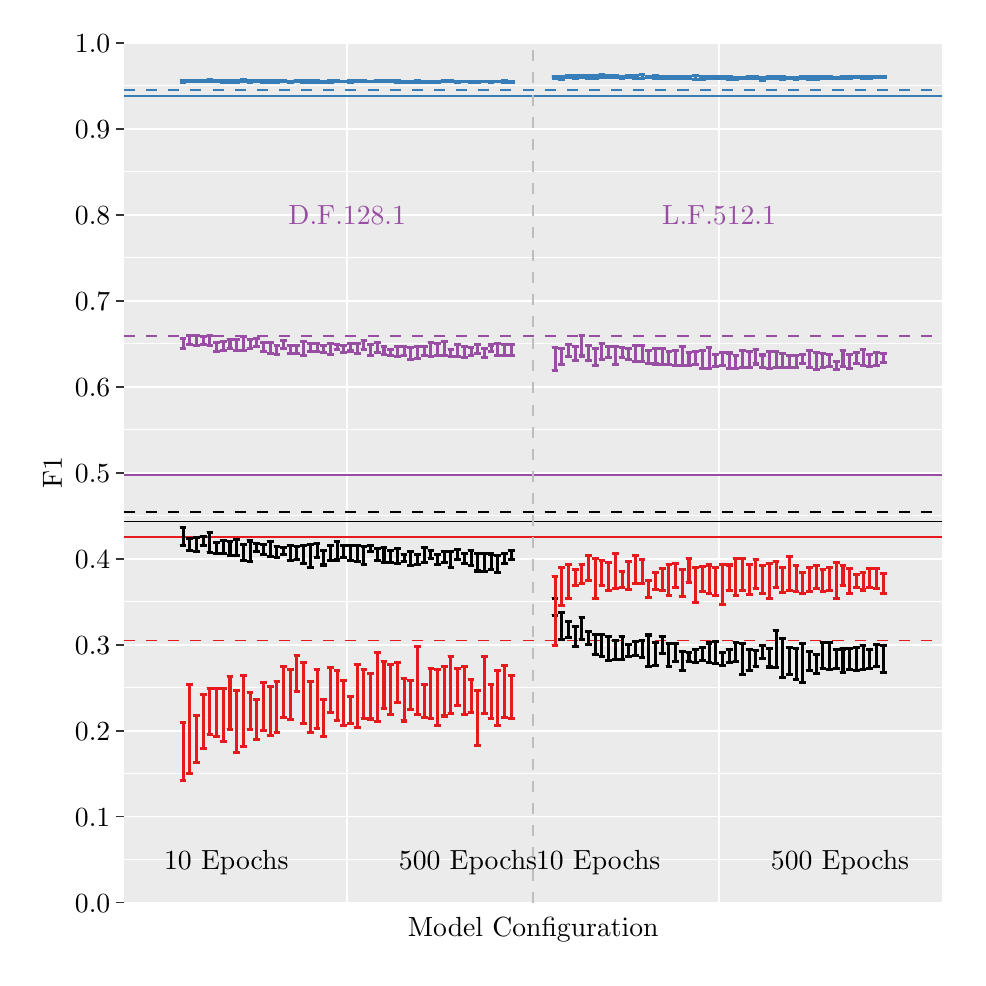
\begin{tikzpicture}[x=1pt,y=1pt]
\definecolor{fillColor}{RGB}{255,255,255}
\path[use as bounding box,fill=fillColor,fill opacity=0.00] (0,0) rectangle (336.00,336.00);
\begin{scope}
\path[clip] (  0.00,  0.00) rectangle (336.00,336.00);
\definecolor{drawColor}{RGB}{255,255,255}
\definecolor{fillColor}{RGB}{255,255,255}

\path[draw=drawColor,line width= 0.6pt,line join=round,line cap=round,fill=fillColor] (  0.00,  0.00) rectangle (336.00,336.00);
\end{scope}
\begin{scope}
\path[clip] ( 34.81, 19.83) rectangle (330.50,330.50);
\definecolor{fillColor}{gray}{0.92}

\path[fill=fillColor] ( 34.81, 19.83) rectangle (330.50,330.50);
\definecolor{drawColor}{RGB}{255,255,255}

\path[draw=drawColor,line width= 0.3pt,line join=round] ( 34.81, 35.36) --
	(330.50, 35.36);

\path[draw=drawColor,line width= 0.3pt,line join=round] ( 34.81, 66.43) --
	(330.50, 66.43);

\path[draw=drawColor,line width= 0.3pt,line join=round] ( 34.81, 97.50) --
	(330.50, 97.50);

\path[draw=drawColor,line width= 0.3pt,line join=round] ( 34.81,128.57) --
	(330.50,128.57);

\path[draw=drawColor,line width= 0.3pt,line join=round] ( 34.81,159.63) --
	(330.50,159.63);

\path[draw=drawColor,line width= 0.3pt,line join=round] ( 34.81,190.70) --
	(330.50,190.70);

\path[draw=drawColor,line width= 0.3pt,line join=round] ( 34.81,221.77) --
	(330.50,221.77);

\path[draw=drawColor,line width= 0.3pt,line join=round] ( 34.81,252.83) --
	(330.50,252.83);

\path[draw=drawColor,line width= 0.3pt,line join=round] ( 34.81,283.90) --
	(330.50,283.90);

\path[draw=drawColor,line width= 0.3pt,line join=round] ( 34.81,314.97) --
	(330.50,314.97);

\path[draw=drawColor,line width= 0.6pt,line join=round] ( 34.81, 19.83) --
	(330.50, 19.83);

\path[draw=drawColor,line width= 0.6pt,line join=round] ( 34.81, 50.90) --
	(330.50, 50.90);

\path[draw=drawColor,line width= 0.6pt,line join=round] ( 34.81, 81.96) --
	(330.50, 81.96);

\path[draw=drawColor,line width= 0.6pt,line join=round] ( 34.81,113.03) --
	(330.50,113.03);

\path[draw=drawColor,line width= 0.6pt,line join=round] ( 34.81,144.10) --
	(330.50,144.10);

\path[draw=drawColor,line width= 0.6pt,line join=round] ( 34.81,175.17) --
	(330.50,175.17);

\path[draw=drawColor,line width= 0.6pt,line join=round] ( 34.81,206.23) --
	(330.50,206.23);

\path[draw=drawColor,line width= 0.6pt,line join=round] ( 34.81,237.30) --
	(330.50,237.30);

\path[draw=drawColor,line width= 0.6pt,line join=round] ( 34.81,268.37) --
	(330.50,268.37);

\path[draw=drawColor,line width= 0.6pt,line join=round] ( 34.81,299.43) --
	(330.50,299.43);

\path[draw=drawColor,line width= 0.6pt,line join=round] ( 34.81,330.50) --
	(330.50,330.50);

\path[draw=drawColor,line width= 0.6pt,line join=round] (115.45, 19.83) --
	(115.45,330.50);

\path[draw=drawColor,line width= 0.6pt,line join=round] (249.86, 19.83) --
	(249.86,330.50);
\definecolor{drawColor}{RGB}{0,0,0}

\path[draw=drawColor,line width= 0.6pt,line join=round] ( 34.81,157.51) -- (330.50,157.51);
\definecolor{drawColor}{RGB}{55,126,184}

\path[draw=drawColor,line width= 0.6pt,line join=round] ( 34.81,311.32) -- (330.50,311.32);
\definecolor{drawColor}{RGB}{228,26,28}

\path[draw=drawColor,line width= 0.6pt,line join=round] ( 34.81,152.03) -- (330.50,152.03);
\definecolor{drawColor}{RGB}{152,78,163}

\path[draw=drawColor,line width= 0.6pt,line join=round] ( 34.81,174.40) -- (330.50,174.40);
\definecolor{drawColor}{RGB}{0,0,0}

\path[draw=drawColor,line width= 0.6pt,dash pattern=on 4pt off 4pt ,line join=round] ( 34.81,160.94) -- (330.50,160.94);
\definecolor{drawColor}{RGB}{55,126,184}

\path[draw=drawColor,line width= 0.6pt,dash pattern=on 4pt off 4pt ,line join=round] ( 34.81,313.44) -- (330.50,313.44);
\definecolor{drawColor}{RGB}{228,26,28}

\path[draw=drawColor,line width= 0.6pt,dash pattern=on 4pt off 4pt ,line join=round] ( 34.81,114.54) -- (330.50,114.54);
\definecolor{drawColor}{RGB}{152,78,163}

\path[draw=drawColor,line width= 0.6pt,dash pattern=on 4pt off 4pt ,line join=round] ( 34.81,224.68) -- (330.50,224.68);
\definecolor{drawColor}{RGB}{190,190,190}

\path[draw=drawColor,line width= 0.6pt,dash pattern=on 4pt off 4pt ,line join=round] (182.65, 19.83) -- (182.65,330.50);
\definecolor{drawColor}{RGB}{0,0,0}

\path[draw=drawColor,line width= 1.1pt,line join=round] (173.51,147.01) --
	(175.93,147.01);

\path[draw=drawColor,line width= 1.1pt,line join=round] (174.72,147.01) --
	(174.72,143.94);

\path[draw=drawColor,line width= 1.1pt,line join=round] (173.51,143.94) --
	(175.93,143.94);

\path[draw=drawColor,line width= 1.1pt,line join=round] (173.51,147.01) --
	(175.93,147.01);

\path[draw=drawColor,line width= 1.1pt,line join=round] (174.72,147.01) --
	(174.72,143.94);

\path[draw=drawColor,line width= 1.1pt,line join=round] (173.51,143.94) --
	(175.93,143.94);

\path[draw=drawColor,line width= 1.1pt,line join=round] (173.51,147.01) --
	(175.93,147.01);

\path[draw=drawColor,line width= 1.1pt,line join=round] (174.72,147.01) --
	(174.72,143.94);

\path[draw=drawColor,line width= 1.1pt,line join=round] (173.51,143.94) --
	(175.93,143.94);

\path[draw=drawColor,line width= 1.1pt,line join=round] (173.51,147.01) --
	(175.93,147.01);

\path[draw=drawColor,line width= 1.1pt,line join=round] (174.72,147.01) --
	(174.72,143.94);

\path[draw=drawColor,line width= 1.1pt,line join=round] (173.51,143.94) --
	(175.93,143.94);

\path[draw=drawColor,line width= 1.1pt,line join=round] (173.51,147.01) --
	(175.93,147.01);

\path[draw=drawColor,line width= 1.1pt,line join=round] (174.72,147.01) --
	(174.72,143.94);

\path[draw=drawColor,line width= 1.1pt,line join=round] (173.51,143.94) --
	(175.93,143.94);

\path[draw=drawColor,line width= 1.1pt,line join=round] (173.51,147.01) --
	(175.93,147.01);

\path[draw=drawColor,line width= 1.1pt,line join=round] (174.72,147.01) --
	(174.72,143.94);

\path[draw=drawColor,line width= 1.1pt,line join=round] (173.51,143.94) --
	(175.93,143.94);

\path[draw=drawColor,line width= 1.1pt,line join=round] (173.51,147.01) --
	(175.93,147.01);

\path[draw=drawColor,line width= 1.1pt,line join=round] (174.72,147.01) --
	(174.72,143.94);

\path[draw=drawColor,line width= 1.1pt,line join=round] (173.51,143.94) --
	(175.93,143.94);

\path[draw=drawColor,line width= 1.1pt,line join=round] (173.51,147.01) --
	(175.93,147.01);

\path[draw=drawColor,line width= 1.1pt,line join=round] (174.72,147.01) --
	(174.72,143.94);

\path[draw=drawColor,line width= 1.1pt,line join=round] (173.51,143.94) --
	(175.93,143.94);

\path[draw=drawColor,line width= 1.1pt,line join=round] (171.09,145.88) --
	(173.51,145.88);

\path[draw=drawColor,line width= 1.1pt,line join=round] (172.30,145.88) --
	(172.30,142.48);

\path[draw=drawColor,line width= 1.1pt,line join=round] (171.09,142.48) --
	(173.51,142.48);

\path[draw=drawColor,line width= 1.1pt,line join=round] (171.09,145.88) --
	(173.51,145.88);

\path[draw=drawColor,line width= 1.1pt,line join=round] (172.30,145.88) --
	(172.30,142.48);

\path[draw=drawColor,line width= 1.1pt,line join=round] (171.09,142.48) --
	(173.51,142.48);

\path[draw=drawColor,line width= 1.1pt,line join=round] (171.09,145.88) --
	(173.51,145.88);

\path[draw=drawColor,line width= 1.1pt,line join=round] (172.30,145.88) --
	(172.30,142.48);

\path[draw=drawColor,line width= 1.1pt,line join=round] (171.09,142.48) --
	(173.51,142.48);

\path[draw=drawColor,line width= 1.1pt,line join=round] (171.09,145.88) --
	(173.51,145.88);

\path[draw=drawColor,line width= 1.1pt,line join=round] (172.30,145.88) --
	(172.30,142.48);

\path[draw=drawColor,line width= 1.1pt,line join=round] (171.09,142.48) --
	(173.51,142.48);

\path[draw=drawColor,line width= 1.1pt,line join=round] (171.09,145.88) --
	(173.51,145.88);

\path[draw=drawColor,line width= 1.1pt,line join=round] (172.30,145.88) --
	(172.30,142.48);

\path[draw=drawColor,line width= 1.1pt,line join=round] (171.09,142.48) --
	(173.51,142.48);

\path[draw=drawColor,line width= 1.1pt,line join=round] (171.09,145.88) --
	(173.51,145.88);

\path[draw=drawColor,line width= 1.1pt,line join=round] (172.30,145.88) --
	(172.30,142.48);

\path[draw=drawColor,line width= 1.1pt,line join=round] (171.09,142.48) --
	(173.51,142.48);

\path[draw=drawColor,line width= 1.1pt,line join=round] (171.09,145.88) --
	(173.51,145.88);

\path[draw=drawColor,line width= 1.1pt,line join=round] (172.30,145.88) --
	(172.30,142.48);

\path[draw=drawColor,line width= 1.1pt,line join=round] (171.09,142.48) --
	(173.51,142.48);

\path[draw=drawColor,line width= 1.1pt,line join=round] (171.09,145.88) --
	(173.51,145.88);

\path[draw=drawColor,line width= 1.1pt,line join=round] (172.30,145.88) --
	(172.30,142.48);

\path[draw=drawColor,line width= 1.1pt,line join=round] (171.09,142.48) --
	(173.51,142.48);

\path[draw=drawColor,line width= 1.1pt,line join=round] (168.67,145.20) --
	(171.09,145.20);

\path[draw=drawColor,line width= 1.1pt,line join=round] (169.88,145.20) --
	(169.88,139.00);

\path[draw=drawColor,line width= 1.1pt,line join=round] (168.67,139.00) --
	(171.09,139.00);

\path[draw=drawColor,line width= 1.1pt,line join=round] (168.67,145.20) --
	(171.09,145.20);

\path[draw=drawColor,line width= 1.1pt,line join=round] (169.88,145.20) --
	(169.88,139.00);

\path[draw=drawColor,line width= 1.1pt,line join=round] (168.67,139.00) --
	(171.09,139.00);

\path[draw=drawColor,line width= 1.1pt,line join=round] (168.67,145.20) --
	(171.09,145.20);

\path[draw=drawColor,line width= 1.1pt,line join=round] (169.88,145.20) --
	(169.88,139.00);

\path[draw=drawColor,line width= 1.1pt,line join=round] (168.67,139.00) --
	(171.09,139.00);

\path[draw=drawColor,line width= 1.1pt,line join=round] (168.67,145.20) --
	(171.09,145.20);

\path[draw=drawColor,line width= 1.1pt,line join=round] (169.88,145.20) --
	(169.88,139.00);

\path[draw=drawColor,line width= 1.1pt,line join=round] (168.67,139.00) --
	(171.09,139.00);

\path[draw=drawColor,line width= 1.1pt,line join=round] (168.67,145.20) --
	(171.09,145.20);

\path[draw=drawColor,line width= 1.1pt,line join=round] (169.88,145.20) --
	(169.88,139.00);

\path[draw=drawColor,line width= 1.1pt,line join=round] (168.67,139.00) --
	(171.09,139.00);

\path[draw=drawColor,line width= 1.1pt,line join=round] (168.67,145.20) --
	(171.09,145.20);

\path[draw=drawColor,line width= 1.1pt,line join=round] (169.88,145.20) --
	(169.88,139.00);

\path[draw=drawColor,line width= 1.1pt,line join=round] (168.67,139.00) --
	(171.09,139.00);

\path[draw=drawColor,line width= 1.1pt,line join=round] (168.67,145.20) --
	(171.09,145.20);

\path[draw=drawColor,line width= 1.1pt,line join=round] (169.88,145.20) --
	(169.88,139.00);

\path[draw=drawColor,line width= 1.1pt,line join=round] (168.67,139.00) --
	(171.09,139.00);

\path[draw=drawColor,line width= 1.1pt,line join=round] (168.67,145.20) --
	(171.09,145.20);

\path[draw=drawColor,line width= 1.1pt,line join=round] (169.88,145.20) --
	(169.88,139.00);

\path[draw=drawColor,line width= 1.1pt,line join=round] (168.67,139.00) --
	(171.09,139.00);

\path[draw=drawColor,line width= 1.1pt,line join=round] (166.26,145.81) --
	(168.67,145.81);

\path[draw=drawColor,line width= 1.1pt,line join=round] (167.46,145.81) --
	(167.46,140.18);

\path[draw=drawColor,line width= 1.1pt,line join=round] (166.26,140.18) --
	(168.67,140.18);

\path[draw=drawColor,line width= 1.1pt,line join=round] (166.26,145.81) --
	(168.67,145.81);

\path[draw=drawColor,line width= 1.1pt,line join=round] (167.46,145.81) --
	(167.46,140.18);

\path[draw=drawColor,line width= 1.1pt,line join=round] (166.26,140.18) --
	(168.67,140.18);

\path[draw=drawColor,line width= 1.1pt,line join=round] (166.26,145.81) --
	(168.67,145.81);

\path[draw=drawColor,line width= 1.1pt,line join=round] (167.46,145.81) --
	(167.46,140.18);

\path[draw=drawColor,line width= 1.1pt,line join=round] (166.26,140.18) --
	(168.67,140.18);

\path[draw=drawColor,line width= 1.1pt,line join=round] (166.26,145.81) --
	(168.67,145.81);

\path[draw=drawColor,line width= 1.1pt,line join=round] (167.46,145.81) --
	(167.46,140.18);

\path[draw=drawColor,line width= 1.1pt,line join=round] (166.26,140.18) --
	(168.67,140.18);

\path[draw=drawColor,line width= 1.1pt,line join=round] (166.26,145.81) --
	(168.67,145.81);

\path[draw=drawColor,line width= 1.1pt,line join=round] (167.46,145.81) --
	(167.46,140.18);

\path[draw=drawColor,line width= 1.1pt,line join=round] (166.26,140.18) --
	(168.67,140.18);

\path[draw=drawColor,line width= 1.1pt,line join=round] (166.26,145.81) --
	(168.67,145.81);

\path[draw=drawColor,line width= 1.1pt,line join=round] (167.46,145.81) --
	(167.46,140.18);

\path[draw=drawColor,line width= 1.1pt,line join=round] (166.26,140.18) --
	(168.67,140.18);

\path[draw=drawColor,line width= 1.1pt,line join=round] (166.26,145.81) --
	(168.67,145.81);

\path[draw=drawColor,line width= 1.1pt,line join=round] (167.46,145.81) --
	(167.46,140.18);

\path[draw=drawColor,line width= 1.1pt,line join=round] (166.26,140.18) --
	(168.67,140.18);

\path[draw=drawColor,line width= 1.1pt,line join=round] (166.26,145.81) --
	(168.67,145.81);

\path[draw=drawColor,line width= 1.1pt,line join=round] (167.46,145.81) --
	(167.46,140.18);

\path[draw=drawColor,line width= 1.1pt,line join=round] (166.26,140.18) --
	(168.67,140.18);

\path[draw=drawColor,line width= 1.1pt,line join=round] (163.84,146.09) --
	(166.26,146.09);

\path[draw=drawColor,line width= 1.1pt,line join=round] (165.05,146.09) --
	(165.05,139.37);

\path[draw=drawColor,line width= 1.1pt,line join=round] (163.84,139.37) --
	(166.26,139.37);

\path[draw=drawColor,line width= 1.1pt,line join=round] (163.84,146.09) --
	(166.26,146.09);

\path[draw=drawColor,line width= 1.1pt,line join=round] (165.05,146.09) --
	(165.05,139.37);

\path[draw=drawColor,line width= 1.1pt,line join=round] (163.84,139.37) --
	(166.26,139.37);

\path[draw=drawColor,line width= 1.1pt,line join=round] (163.84,146.09) --
	(166.26,146.09);

\path[draw=drawColor,line width= 1.1pt,line join=round] (165.05,146.09) --
	(165.05,139.37);

\path[draw=drawColor,line width= 1.1pt,line join=round] (163.84,139.37) --
	(166.26,139.37);

\path[draw=drawColor,line width= 1.1pt,line join=round] (163.84,146.09) --
	(166.26,146.09);

\path[draw=drawColor,line width= 1.1pt,line join=round] (165.05,146.09) --
	(165.05,139.37);

\path[draw=drawColor,line width= 1.1pt,line join=round] (163.84,139.37) --
	(166.26,139.37);

\path[draw=drawColor,line width= 1.1pt,line join=round] (163.84,146.09) --
	(166.26,146.09);

\path[draw=drawColor,line width= 1.1pt,line join=round] (165.05,146.09) --
	(165.05,139.37);

\path[draw=drawColor,line width= 1.1pt,line join=round] (163.84,139.37) --
	(166.26,139.37);

\path[draw=drawColor,line width= 1.1pt,line join=round] (163.84,146.09) --
	(166.26,146.09);

\path[draw=drawColor,line width= 1.1pt,line join=round] (165.05,146.09) --
	(165.05,139.37);

\path[draw=drawColor,line width= 1.1pt,line join=round] (163.84,139.37) --
	(166.26,139.37);

\path[draw=drawColor,line width= 1.1pt,line join=round] (163.84,146.09) --
	(166.26,146.09);

\path[draw=drawColor,line width= 1.1pt,line join=round] (165.05,146.09) --
	(165.05,139.37);

\path[draw=drawColor,line width= 1.1pt,line join=round] (163.84,139.37) --
	(166.26,139.37);

\path[draw=drawColor,line width= 1.1pt,line join=round] (163.84,146.09) --
	(166.26,146.09);

\path[draw=drawColor,line width= 1.1pt,line join=round] (165.05,146.09) --
	(165.05,139.37);

\path[draw=drawColor,line width= 1.1pt,line join=round] (163.84,139.37) --
	(166.26,139.37);

\path[draw=drawColor,line width= 1.1pt,line join=round] (161.42,145.88) --
	(163.84,145.88);

\path[draw=drawColor,line width= 1.1pt,line join=round] (162.63,145.88) --
	(162.63,139.67);

\path[draw=drawColor,line width= 1.1pt,line join=round] (161.42,139.67) --
	(163.84,139.67);

\path[draw=drawColor,line width= 1.1pt,line join=round] (161.42,145.88) --
	(163.84,145.88);

\path[draw=drawColor,line width= 1.1pt,line join=round] (162.63,145.88) --
	(162.63,139.67);

\path[draw=drawColor,line width= 1.1pt,line join=round] (161.42,139.67) --
	(163.84,139.67);

\path[draw=drawColor,line width= 1.1pt,line join=round] (161.42,145.88) --
	(163.84,145.88);

\path[draw=drawColor,line width= 1.1pt,line join=round] (162.63,145.88) --
	(162.63,139.67);

\path[draw=drawColor,line width= 1.1pt,line join=round] (161.42,139.67) --
	(163.84,139.67);

\path[draw=drawColor,line width= 1.1pt,line join=round] (161.42,145.88) --
	(163.84,145.88);

\path[draw=drawColor,line width= 1.1pt,line join=round] (162.63,145.88) --
	(162.63,139.67);

\path[draw=drawColor,line width= 1.1pt,line join=round] (161.42,139.67) --
	(163.84,139.67);

\path[draw=drawColor,line width= 1.1pt,line join=round] (161.42,145.88) --
	(163.84,145.88);

\path[draw=drawColor,line width= 1.1pt,line join=round] (162.63,145.88) --
	(162.63,139.67);

\path[draw=drawColor,line width= 1.1pt,line join=round] (161.42,139.67) --
	(163.84,139.67);

\path[draw=drawColor,line width= 1.1pt,line join=round] (161.42,145.88) --
	(163.84,145.88);

\path[draw=drawColor,line width= 1.1pt,line join=round] (162.63,145.88) --
	(162.63,139.67);

\path[draw=drawColor,line width= 1.1pt,line join=round] (161.42,139.67) --
	(163.84,139.67);

\path[draw=drawColor,line width= 1.1pt,line join=round] (161.42,145.88) --
	(163.84,145.88);

\path[draw=drawColor,line width= 1.1pt,line join=round] (162.63,145.88) --
	(162.63,139.67);

\path[draw=drawColor,line width= 1.1pt,line join=round] (161.42,139.67) --
	(163.84,139.67);

\path[draw=drawColor,line width= 1.1pt,line join=round] (161.42,145.88) --
	(163.84,145.88);

\path[draw=drawColor,line width= 1.1pt,line join=round] (162.63,145.88) --
	(162.63,139.67);

\path[draw=drawColor,line width= 1.1pt,line join=round] (161.42,139.67) --
	(163.84,139.67);

\path[draw=drawColor,line width= 1.1pt,line join=round] (159.00,147.08) --
	(161.42,147.08);

\path[draw=drawColor,line width= 1.1pt,line join=round] (160.21,147.08) --
	(160.21,141.58);

\path[draw=drawColor,line width= 1.1pt,line join=round] (159.00,141.58) --
	(161.42,141.58);

\path[draw=drawColor,line width= 1.1pt,line join=round] (159.00,147.08) --
	(161.42,147.08);

\path[draw=drawColor,line width= 1.1pt,line join=round] (160.21,147.08) --
	(160.21,141.58);

\path[draw=drawColor,line width= 1.1pt,line join=round] (159.00,141.58) --
	(161.42,141.58);

\path[draw=drawColor,line width= 1.1pt,line join=round] (159.00,147.08) --
	(161.42,147.08);

\path[draw=drawColor,line width= 1.1pt,line join=round] (160.21,147.08) --
	(160.21,141.58);

\path[draw=drawColor,line width= 1.1pt,line join=round] (159.00,141.58) --
	(161.42,141.58);

\path[draw=drawColor,line width= 1.1pt,line join=round] (159.00,147.08) --
	(161.42,147.08);

\path[draw=drawColor,line width= 1.1pt,line join=round] (160.21,147.08) --
	(160.21,141.58);

\path[draw=drawColor,line width= 1.1pt,line join=round] (159.00,141.58) --
	(161.42,141.58);

\path[draw=drawColor,line width= 1.1pt,line join=round] (159.00,147.08) --
	(161.42,147.08);

\path[draw=drawColor,line width= 1.1pt,line join=round] (160.21,147.08) --
	(160.21,141.58);

\path[draw=drawColor,line width= 1.1pt,line join=round] (159.00,141.58) --
	(161.42,141.58);

\path[draw=drawColor,line width= 1.1pt,line join=round] (159.00,147.08) --
	(161.42,147.08);

\path[draw=drawColor,line width= 1.1pt,line join=round] (160.21,147.08) --
	(160.21,141.58);

\path[draw=drawColor,line width= 1.1pt,line join=round] (159.00,141.58) --
	(161.42,141.58);

\path[draw=drawColor,line width= 1.1pt,line join=round] (159.00,147.08) --
	(161.42,147.08);

\path[draw=drawColor,line width= 1.1pt,line join=round] (160.21,147.08) --
	(160.21,141.58);

\path[draw=drawColor,line width= 1.1pt,line join=round] (159.00,141.58) --
	(161.42,141.58);

\path[draw=drawColor,line width= 1.1pt,line join=round] (159.00,147.08) --
	(161.42,147.08);

\path[draw=drawColor,line width= 1.1pt,line join=round] (160.21,147.08) --
	(160.21,141.58);

\path[draw=drawColor,line width= 1.1pt,line join=round] (159.00,141.58) --
	(161.42,141.58);

\path[draw=drawColor,line width= 1.1pt,line join=round] (156.58,146.00) --
	(159.00,146.00);

\path[draw=drawColor,line width= 1.1pt,line join=round] (157.79,146.00) --
	(157.79,142.24);

\path[draw=drawColor,line width= 1.1pt,line join=round] (156.58,142.24) --
	(159.00,142.24);

\path[draw=drawColor,line width= 1.1pt,line join=round] (156.58,146.00) --
	(159.00,146.00);

\path[draw=drawColor,line width= 1.1pt,line join=round] (157.79,146.00) --
	(157.79,142.24);

\path[draw=drawColor,line width= 1.1pt,line join=round] (156.58,142.24) --
	(159.00,142.24);

\path[draw=drawColor,line width= 1.1pt,line join=round] (156.58,146.00) --
	(159.00,146.00);

\path[draw=drawColor,line width= 1.1pt,line join=round] (157.79,146.00) --
	(157.79,142.24);

\path[draw=drawColor,line width= 1.1pt,line join=round] (156.58,142.24) --
	(159.00,142.24);

\path[draw=drawColor,line width= 1.1pt,line join=round] (156.58,146.00) --
	(159.00,146.00);

\path[draw=drawColor,line width= 1.1pt,line join=round] (157.79,146.00) --
	(157.79,142.24);

\path[draw=drawColor,line width= 1.1pt,line join=round] (156.58,142.24) --
	(159.00,142.24);

\path[draw=drawColor,line width= 1.1pt,line join=round] (156.58,146.00) --
	(159.00,146.00);

\path[draw=drawColor,line width= 1.1pt,line join=round] (157.79,146.00) --
	(157.79,142.24);

\path[draw=drawColor,line width= 1.1pt,line join=round] (156.58,142.24) --
	(159.00,142.24);

\path[draw=drawColor,line width= 1.1pt,line join=round] (156.58,146.00) --
	(159.00,146.00);

\path[draw=drawColor,line width= 1.1pt,line join=round] (157.79,146.00) --
	(157.79,142.24);

\path[draw=drawColor,line width= 1.1pt,line join=round] (156.58,142.24) --
	(159.00,142.24);

\path[draw=drawColor,line width= 1.1pt,line join=round] (156.58,146.00) --
	(159.00,146.00);

\path[draw=drawColor,line width= 1.1pt,line join=round] (157.79,146.00) --
	(157.79,142.24);

\path[draw=drawColor,line width= 1.1pt,line join=round] (156.58,142.24) --
	(159.00,142.24);

\path[draw=drawColor,line width= 1.1pt,line join=round] (156.58,146.00) --
	(159.00,146.00);

\path[draw=drawColor,line width= 1.1pt,line join=round] (157.79,146.00) --
	(157.79,142.24);

\path[draw=drawColor,line width= 1.1pt,line join=round] (156.58,142.24) --
	(159.00,142.24);

\path[draw=drawColor,line width= 1.1pt,line join=round] (154.16,147.31) --
	(156.58,147.31);

\path[draw=drawColor,line width= 1.1pt,line join=round] (155.37,147.31) --
	(155.37,143.92);

\path[draw=drawColor,line width= 1.1pt,line join=round] (154.16,143.92) --
	(156.58,143.92);

\path[draw=drawColor,line width= 1.1pt,line join=round] (154.16,147.31) --
	(156.58,147.31);

\path[draw=drawColor,line width= 1.1pt,line join=round] (155.37,147.31) --
	(155.37,143.92);

\path[draw=drawColor,line width= 1.1pt,line join=round] (154.16,143.92) --
	(156.58,143.92);

\path[draw=drawColor,line width= 1.1pt,line join=round] (154.16,147.31) --
	(156.58,147.31);

\path[draw=drawColor,line width= 1.1pt,line join=round] (155.37,147.31) --
	(155.37,143.92);

\path[draw=drawColor,line width= 1.1pt,line join=round] (154.16,143.92) --
	(156.58,143.92);

\path[draw=drawColor,line width= 1.1pt,line join=round] (154.16,147.31) --
	(156.58,147.31);

\path[draw=drawColor,line width= 1.1pt,line join=round] (155.37,147.31) --
	(155.37,143.92);

\path[draw=drawColor,line width= 1.1pt,line join=round] (154.16,143.92) --
	(156.58,143.92);

\path[draw=drawColor,line width= 1.1pt,line join=round] (154.16,147.31) --
	(156.58,147.31);

\path[draw=drawColor,line width= 1.1pt,line join=round] (155.37,147.31) --
	(155.37,143.92);

\path[draw=drawColor,line width= 1.1pt,line join=round] (154.16,143.92) --
	(156.58,143.92);

\path[draw=drawColor,line width= 1.1pt,line join=round] (154.16,147.31) --
	(156.58,147.31);

\path[draw=drawColor,line width= 1.1pt,line join=round] (155.37,147.31) --
	(155.37,143.92);

\path[draw=drawColor,line width= 1.1pt,line join=round] (154.16,143.92) --
	(156.58,143.92);

\path[draw=drawColor,line width= 1.1pt,line join=round] (154.16,147.31) --
	(156.58,147.31);

\path[draw=drawColor,line width= 1.1pt,line join=round] (155.37,147.31) --
	(155.37,143.92);

\path[draw=drawColor,line width= 1.1pt,line join=round] (154.16,143.92) --
	(156.58,143.92);

\path[draw=drawColor,line width= 1.1pt,line join=round] (154.16,147.31) --
	(156.58,147.31);

\path[draw=drawColor,line width= 1.1pt,line join=round] (155.37,147.31) --
	(155.37,143.92);

\path[draw=drawColor,line width= 1.1pt,line join=round] (154.16,143.92) --
	(156.58,143.92);

\path[draw=drawColor,line width= 1.1pt,line join=round] (151.74,146.73) --
	(154.16,146.73);

\path[draw=drawColor,line width= 1.1pt,line join=round] (152.95,146.73) --
	(152.95,140.78);

\path[draw=drawColor,line width= 1.1pt,line join=round] (151.74,140.78) --
	(154.16,140.78);

\path[draw=drawColor,line width= 1.1pt,line join=round] (151.74,146.73) --
	(154.16,146.73);

\path[draw=drawColor,line width= 1.1pt,line join=round] (152.95,146.73) --
	(152.95,140.78);

\path[draw=drawColor,line width= 1.1pt,line join=round] (151.74,140.78) --
	(154.16,140.78);

\path[draw=drawColor,line width= 1.1pt,line join=round] (151.74,146.73) --
	(154.16,146.73);

\path[draw=drawColor,line width= 1.1pt,line join=round] (152.95,146.73) --
	(152.95,140.78);

\path[draw=drawColor,line width= 1.1pt,line join=round] (151.74,140.78) --
	(154.16,140.78);

\path[draw=drawColor,line width= 1.1pt,line join=round] (151.74,146.73) --
	(154.16,146.73);

\path[draw=drawColor,line width= 1.1pt,line join=round] (152.95,146.73) --
	(152.95,140.78);

\path[draw=drawColor,line width= 1.1pt,line join=round] (151.74,140.78) --
	(154.16,140.78);

\path[draw=drawColor,line width= 1.1pt,line join=round] (151.74,146.73) --
	(154.16,146.73);

\path[draw=drawColor,line width= 1.1pt,line join=round] (152.95,146.73) --
	(152.95,140.78);

\path[draw=drawColor,line width= 1.1pt,line join=round] (151.74,140.78) --
	(154.16,140.78);

\path[draw=drawColor,line width= 1.1pt,line join=round] (151.74,146.73) --
	(154.16,146.73);

\path[draw=drawColor,line width= 1.1pt,line join=round] (152.95,146.73) --
	(152.95,140.78);

\path[draw=drawColor,line width= 1.1pt,line join=round] (151.74,140.78) --
	(154.16,140.78);

\path[draw=drawColor,line width= 1.1pt,line join=round] (151.74,146.73) --
	(154.16,146.73);

\path[draw=drawColor,line width= 1.1pt,line join=round] (152.95,146.73) --
	(152.95,140.78);

\path[draw=drawColor,line width= 1.1pt,line join=round] (151.74,140.78) --
	(154.16,140.78);

\path[draw=drawColor,line width= 1.1pt,line join=round] (151.74,146.73) --
	(154.16,146.73);

\path[draw=drawColor,line width= 1.1pt,line join=round] (152.95,146.73) --
	(152.95,140.78);

\path[draw=drawColor,line width= 1.1pt,line join=round] (151.74,140.78) --
	(154.16,140.78);

\path[draw=drawColor,line width= 1.1pt,line join=round] (149.32,146.57) --
	(151.74,146.57);

\path[draw=drawColor,line width= 1.1pt,line join=round] (150.53,146.57) --
	(150.53,142.76);

\path[draw=drawColor,line width= 1.1pt,line join=round] (149.32,142.76) --
	(151.74,142.76);

\path[draw=drawColor,line width= 1.1pt,line join=round] (149.32,146.57) --
	(151.74,146.57);

\path[draw=drawColor,line width= 1.1pt,line join=round] (150.53,146.57) --
	(150.53,142.76);

\path[draw=drawColor,line width= 1.1pt,line join=round] (149.32,142.76) --
	(151.74,142.76);

\path[draw=drawColor,line width= 1.1pt,line join=round] (149.32,146.57) --
	(151.74,146.57);

\path[draw=drawColor,line width= 1.1pt,line join=round] (150.53,146.57) --
	(150.53,142.76);

\path[draw=drawColor,line width= 1.1pt,line join=round] (149.32,142.76) --
	(151.74,142.76);

\path[draw=drawColor,line width= 1.1pt,line join=round] (149.32,146.57) --
	(151.74,146.57);

\path[draw=drawColor,line width= 1.1pt,line join=round] (150.53,146.57) --
	(150.53,142.76);

\path[draw=drawColor,line width= 1.1pt,line join=round] (149.32,142.76) --
	(151.74,142.76);

\path[draw=drawColor,line width= 1.1pt,line join=round] (149.32,146.57) --
	(151.74,146.57);

\path[draw=drawColor,line width= 1.1pt,line join=round] (150.53,146.57) --
	(150.53,142.76);

\path[draw=drawColor,line width= 1.1pt,line join=round] (149.32,142.76) --
	(151.74,142.76);

\path[draw=drawColor,line width= 1.1pt,line join=round] (149.32,146.57) --
	(151.74,146.57);

\path[draw=drawColor,line width= 1.1pt,line join=round] (150.53,146.57) --
	(150.53,142.76);

\path[draw=drawColor,line width= 1.1pt,line join=round] (149.32,142.76) --
	(151.74,142.76);

\path[draw=drawColor,line width= 1.1pt,line join=round] (149.32,146.57) --
	(151.74,146.57);

\path[draw=drawColor,line width= 1.1pt,line join=round] (150.53,146.57) --
	(150.53,142.76);

\path[draw=drawColor,line width= 1.1pt,line join=round] (149.32,142.76) --
	(151.74,142.76);

\path[draw=drawColor,line width= 1.1pt,line join=round] (149.32,146.57) --
	(151.74,146.57);

\path[draw=drawColor,line width= 1.1pt,line join=round] (150.53,146.57) --
	(150.53,142.76);

\path[draw=drawColor,line width= 1.1pt,line join=round] (149.32,142.76) --
	(151.74,142.76);

\path[draw=drawColor,line width= 1.1pt,line join=round] (146.90,145.61) --
	(149.32,145.61);

\path[draw=drawColor,line width= 1.1pt,line join=round] (148.11,145.61) --
	(148.11,141.94);

\path[draw=drawColor,line width= 1.1pt,line join=round] (146.90,141.94) --
	(149.32,141.94);

\path[draw=drawColor,line width= 1.1pt,line join=round] (146.90,145.61) --
	(149.32,145.61);

\path[draw=drawColor,line width= 1.1pt,line join=round] (148.11,145.61) --
	(148.11,141.94);

\path[draw=drawColor,line width= 1.1pt,line join=round] (146.90,141.94) --
	(149.32,141.94);

\path[draw=drawColor,line width= 1.1pt,line join=round] (146.90,145.61) --
	(149.32,145.61);

\path[draw=drawColor,line width= 1.1pt,line join=round] (148.11,145.61) --
	(148.11,141.94);

\path[draw=drawColor,line width= 1.1pt,line join=round] (146.90,141.94) --
	(149.32,141.94);

\path[draw=drawColor,line width= 1.1pt,line join=round] (146.90,145.61) --
	(149.32,145.61);

\path[draw=drawColor,line width= 1.1pt,line join=round] (148.11,145.61) --
	(148.11,141.94);

\path[draw=drawColor,line width= 1.1pt,line join=round] (146.90,141.94) --
	(149.32,141.94);

\path[draw=drawColor,line width= 1.1pt,line join=round] (146.90,145.61) --
	(149.32,145.61);

\path[draw=drawColor,line width= 1.1pt,line join=round] (148.11,145.61) --
	(148.11,141.94);

\path[draw=drawColor,line width= 1.1pt,line join=round] (146.90,141.94) --
	(149.32,141.94);

\path[draw=drawColor,line width= 1.1pt,line join=round] (146.90,145.61) --
	(149.32,145.61);

\path[draw=drawColor,line width= 1.1pt,line join=round] (148.11,145.61) --
	(148.11,141.94);

\path[draw=drawColor,line width= 1.1pt,line join=round] (146.90,141.94) --
	(149.32,141.94);

\path[draw=drawColor,line width= 1.1pt,line join=round] (146.90,145.61) --
	(149.32,145.61);

\path[draw=drawColor,line width= 1.1pt,line join=round] (148.11,145.61) --
	(148.11,141.94);

\path[draw=drawColor,line width= 1.1pt,line join=round] (146.90,141.94) --
	(149.32,141.94);

\path[draw=drawColor,line width= 1.1pt,line join=round] (146.90,145.61) --
	(149.32,145.61);

\path[draw=drawColor,line width= 1.1pt,line join=round] (148.11,145.61) --
	(148.11,141.94);

\path[draw=drawColor,line width= 1.1pt,line join=round] (146.90,141.94) --
	(149.32,141.94);

\path[draw=drawColor,line width= 1.1pt,line join=round] (144.48,147.13) --
	(146.90,147.13);

\path[draw=drawColor,line width= 1.1pt,line join=round] (145.69,147.13) --
	(145.69,144.16);

\path[draw=drawColor,line width= 1.1pt,line join=round] (144.48,144.16) --
	(146.90,144.16);

\path[draw=drawColor,line width= 1.1pt,line join=round] (144.48,147.13) --
	(146.90,147.13);

\path[draw=drawColor,line width= 1.1pt,line join=round] (145.69,147.13) --
	(145.69,144.16);

\path[draw=drawColor,line width= 1.1pt,line join=round] (144.48,144.16) --
	(146.90,144.16);

\path[draw=drawColor,line width= 1.1pt,line join=round] (144.48,147.13) --
	(146.90,147.13);

\path[draw=drawColor,line width= 1.1pt,line join=round] (145.69,147.13) --
	(145.69,144.16);

\path[draw=drawColor,line width= 1.1pt,line join=round] (144.48,144.16) --
	(146.90,144.16);

\path[draw=drawColor,line width= 1.1pt,line join=round] (144.48,147.13) --
	(146.90,147.13);

\path[draw=drawColor,line width= 1.1pt,line join=round] (145.69,147.13) --
	(145.69,144.16);

\path[draw=drawColor,line width= 1.1pt,line join=round] (144.48,144.16) --
	(146.90,144.16);

\path[draw=drawColor,line width= 1.1pt,line join=round] (144.48,147.13) --
	(146.90,147.13);

\path[draw=drawColor,line width= 1.1pt,line join=round] (145.69,147.13) --
	(145.69,144.16);

\path[draw=drawColor,line width= 1.1pt,line join=round] (144.48,144.16) --
	(146.90,144.16);

\path[draw=drawColor,line width= 1.1pt,line join=round] (144.48,147.13) --
	(146.90,147.13);

\path[draw=drawColor,line width= 1.1pt,line join=round] (145.69,147.13) --
	(145.69,144.16);

\path[draw=drawColor,line width= 1.1pt,line join=round] (144.48,144.16) --
	(146.90,144.16);

\path[draw=drawColor,line width= 1.1pt,line join=round] (144.48,147.13) --
	(146.90,147.13);

\path[draw=drawColor,line width= 1.1pt,line join=round] (145.69,147.13) --
	(145.69,144.16);

\path[draw=drawColor,line width= 1.1pt,line join=round] (144.48,144.16) --
	(146.90,144.16);

\path[draw=drawColor,line width= 1.1pt,line join=round] (144.48,147.13) --
	(146.90,147.13);

\path[draw=drawColor,line width= 1.1pt,line join=round] (145.69,147.13) --
	(145.69,144.16);

\path[draw=drawColor,line width= 1.1pt,line join=round] (144.48,144.16) --
	(146.90,144.16);

\path[draw=drawColor,line width= 1.1pt,line join=round] (142.06,148.08) --
	(144.48,148.08);

\path[draw=drawColor,line width= 1.1pt,line join=round] (143.27,148.08) --
	(143.27,142.70);

\path[draw=drawColor,line width= 1.1pt,line join=round] (142.06,142.70) --
	(144.48,142.70);

\path[draw=drawColor,line width= 1.1pt,line join=round] (142.06,148.08) --
	(144.48,148.08);

\path[draw=drawColor,line width= 1.1pt,line join=round] (143.27,148.08) --
	(143.27,142.70);

\path[draw=drawColor,line width= 1.1pt,line join=round] (142.06,142.70) --
	(144.48,142.70);

\path[draw=drawColor,line width= 1.1pt,line join=round] (142.06,148.08) --
	(144.48,148.08);

\path[draw=drawColor,line width= 1.1pt,line join=round] (143.27,148.08) --
	(143.27,142.70);

\path[draw=drawColor,line width= 1.1pt,line join=round] (142.06,142.70) --
	(144.48,142.70);

\path[draw=drawColor,line width= 1.1pt,line join=round] (142.06,148.08) --
	(144.48,148.08);

\path[draw=drawColor,line width= 1.1pt,line join=round] (143.27,148.08) --
	(143.27,142.70);

\path[draw=drawColor,line width= 1.1pt,line join=round] (142.06,142.70) --
	(144.48,142.70);

\path[draw=drawColor,line width= 1.1pt,line join=round] (142.06,148.08) --
	(144.48,148.08);

\path[draw=drawColor,line width= 1.1pt,line join=round] (143.27,148.08) --
	(143.27,142.70);

\path[draw=drawColor,line width= 1.1pt,line join=round] (142.06,142.70) --
	(144.48,142.70);

\path[draw=drawColor,line width= 1.1pt,line join=round] (142.06,148.08) --
	(144.48,148.08);

\path[draw=drawColor,line width= 1.1pt,line join=round] (143.27,148.08) --
	(143.27,142.70);

\path[draw=drawColor,line width= 1.1pt,line join=round] (142.06,142.70) --
	(144.48,142.70);

\path[draw=drawColor,line width= 1.1pt,line join=round] (142.06,148.08) --
	(144.48,148.08);

\path[draw=drawColor,line width= 1.1pt,line join=round] (143.27,148.08) --
	(143.27,142.70);

\path[draw=drawColor,line width= 1.1pt,line join=round] (142.06,142.70) --
	(144.48,142.70);

\path[draw=drawColor,line width= 1.1pt,line join=round] (142.06,148.08) --
	(144.48,148.08);

\path[draw=drawColor,line width= 1.1pt,line join=round] (143.27,148.08) --
	(143.27,142.70);

\path[draw=drawColor,line width= 1.1pt,line join=round] (142.06,142.70) --
	(144.48,142.70);

\path[draw=drawColor,line width= 1.1pt,line join=round] (139.64,145.53) --
	(142.06,145.53);

\path[draw=drawColor,line width= 1.1pt,line join=round] (140.85,145.53) --
	(140.85,141.96);

\path[draw=drawColor,line width= 1.1pt,line join=round] (139.64,141.96) --
	(142.06,141.96);

\path[draw=drawColor,line width= 1.1pt,line join=round] (139.64,145.53) --
	(142.06,145.53);

\path[draw=drawColor,line width= 1.1pt,line join=round] (140.85,145.53) --
	(140.85,141.96);

\path[draw=drawColor,line width= 1.1pt,line join=round] (139.64,141.96) --
	(142.06,141.96);

\path[draw=drawColor,line width= 1.1pt,line join=round] (139.64,145.53) --
	(142.06,145.53);

\path[draw=drawColor,line width= 1.1pt,line join=round] (140.85,145.53) --
	(140.85,141.96);

\path[draw=drawColor,line width= 1.1pt,line join=round] (139.64,141.96) --
	(142.06,141.96);

\path[draw=drawColor,line width= 1.1pt,line join=round] (139.64,145.53) --
	(142.06,145.53);

\path[draw=drawColor,line width= 1.1pt,line join=round] (140.85,145.53) --
	(140.85,141.96);

\path[draw=drawColor,line width= 1.1pt,line join=round] (139.64,141.96) --
	(142.06,141.96);

\path[draw=drawColor,line width= 1.1pt,line join=round] (139.64,145.53) --
	(142.06,145.53);

\path[draw=drawColor,line width= 1.1pt,line join=round] (140.85,145.53) --
	(140.85,141.96);

\path[draw=drawColor,line width= 1.1pt,line join=round] (139.64,141.96) --
	(142.06,141.96);

\path[draw=drawColor,line width= 1.1pt,line join=round] (139.64,145.53) --
	(142.06,145.53);

\path[draw=drawColor,line width= 1.1pt,line join=round] (140.85,145.53) --
	(140.85,141.96);

\path[draw=drawColor,line width= 1.1pt,line join=round] (139.64,141.96) --
	(142.06,141.96);

\path[draw=drawColor,line width= 1.1pt,line join=round] (139.64,145.53) --
	(142.06,145.53);

\path[draw=drawColor,line width= 1.1pt,line join=round] (140.85,145.53) --
	(140.85,141.96);

\path[draw=drawColor,line width= 1.1pt,line join=round] (139.64,141.96) --
	(142.06,141.96);

\path[draw=drawColor,line width= 1.1pt,line join=round] (139.64,145.53) --
	(142.06,145.53);

\path[draw=drawColor,line width= 1.1pt,line join=round] (140.85,145.53) --
	(140.85,141.96);

\path[draw=drawColor,line width= 1.1pt,line join=round] (139.64,141.96) --
	(142.06,141.96);

\path[draw=drawColor,line width= 1.1pt,line join=round] (137.22,146.71) --
	(139.64,146.71);

\path[draw=drawColor,line width= 1.1pt,line join=round] (138.43,146.71) --
	(138.43,141.65);

\path[draw=drawColor,line width= 1.1pt,line join=round] (137.22,141.65) --
	(139.64,141.65);

\path[draw=drawColor,line width= 1.1pt,line join=round] (137.22,146.71) --
	(139.64,146.71);

\path[draw=drawColor,line width= 1.1pt,line join=round] (138.43,146.71) --
	(138.43,141.65);

\path[draw=drawColor,line width= 1.1pt,line join=round] (137.22,141.65) --
	(139.64,141.65);

\path[draw=drawColor,line width= 1.1pt,line join=round] (137.22,146.71) --
	(139.64,146.71);

\path[draw=drawColor,line width= 1.1pt,line join=round] (138.43,146.71) --
	(138.43,141.65);

\path[draw=drawColor,line width= 1.1pt,line join=round] (137.22,141.65) --
	(139.64,141.65);

\path[draw=drawColor,line width= 1.1pt,line join=round] (137.22,146.71) --
	(139.64,146.71);

\path[draw=drawColor,line width= 1.1pt,line join=round] (138.43,146.71) --
	(138.43,141.65);

\path[draw=drawColor,line width= 1.1pt,line join=round] (137.22,141.65) --
	(139.64,141.65);

\path[draw=drawColor,line width= 1.1pt,line join=round] (137.22,146.71) --
	(139.64,146.71);

\path[draw=drawColor,line width= 1.1pt,line join=round] (138.43,146.71) --
	(138.43,141.65);

\path[draw=drawColor,line width= 1.1pt,line join=round] (137.22,141.65) --
	(139.64,141.65);

\path[draw=drawColor,line width= 1.1pt,line join=round] (137.22,146.71) --
	(139.64,146.71);

\path[draw=drawColor,line width= 1.1pt,line join=round] (138.43,146.71) --
	(138.43,141.65);

\path[draw=drawColor,line width= 1.1pt,line join=round] (137.22,141.65) --
	(139.64,141.65);

\path[draw=drawColor,line width= 1.1pt,line join=round] (137.22,146.71) --
	(139.64,146.71);

\path[draw=drawColor,line width= 1.1pt,line join=round] (138.43,146.71) --
	(138.43,141.65);

\path[draw=drawColor,line width= 1.1pt,line join=round] (137.22,141.65) --
	(139.64,141.65);

\path[draw=drawColor,line width= 1.1pt,line join=round] (137.22,146.71) --
	(139.64,146.71);

\path[draw=drawColor,line width= 1.1pt,line join=round] (138.43,146.71) --
	(138.43,141.65);

\path[draw=drawColor,line width= 1.1pt,line join=round] (137.22,141.65) --
	(139.64,141.65);

\path[draw=drawColor,line width= 1.1pt,line join=round] (134.80,145.80) --
	(137.22,145.80);

\path[draw=drawColor,line width= 1.1pt,line join=round] (136.01,145.80) --
	(136.01,143.05);

\path[draw=drawColor,line width= 1.1pt,line join=round] (134.80,143.05) --
	(137.22,143.05);

\path[draw=drawColor,line width= 1.1pt,line join=round] (134.80,145.80) --
	(137.22,145.80);

\path[draw=drawColor,line width= 1.1pt,line join=round] (136.01,145.80) --
	(136.01,143.05);

\path[draw=drawColor,line width= 1.1pt,line join=round] (134.80,143.05) --
	(137.22,143.05);

\path[draw=drawColor,line width= 1.1pt,line join=round] (134.80,145.80) --
	(137.22,145.80);

\path[draw=drawColor,line width= 1.1pt,line join=round] (136.01,145.80) --
	(136.01,143.05);

\path[draw=drawColor,line width= 1.1pt,line join=round] (134.80,143.05) --
	(137.22,143.05);

\path[draw=drawColor,line width= 1.1pt,line join=round] (134.80,145.80) --
	(137.22,145.80);

\path[draw=drawColor,line width= 1.1pt,line join=round] (136.01,145.80) --
	(136.01,143.05);

\path[draw=drawColor,line width= 1.1pt,line join=round] (134.80,143.05) --
	(137.22,143.05);

\path[draw=drawColor,line width= 1.1pt,line join=round] (134.80,145.80) --
	(137.22,145.80);

\path[draw=drawColor,line width= 1.1pt,line join=round] (136.01,145.80) --
	(136.01,143.05);

\path[draw=drawColor,line width= 1.1pt,line join=round] (134.80,143.05) --
	(137.22,143.05);

\path[draw=drawColor,line width= 1.1pt,line join=round] (134.80,145.80) --
	(137.22,145.80);

\path[draw=drawColor,line width= 1.1pt,line join=round] (136.01,145.80) --
	(136.01,143.05);

\path[draw=drawColor,line width= 1.1pt,line join=round] (134.80,143.05) --
	(137.22,143.05);

\path[draw=drawColor,line width= 1.1pt,line join=round] (134.80,145.80) --
	(137.22,145.80);

\path[draw=drawColor,line width= 1.1pt,line join=round] (136.01,145.80) --
	(136.01,143.05);

\path[draw=drawColor,line width= 1.1pt,line join=round] (134.80,143.05) --
	(137.22,143.05);

\path[draw=drawColor,line width= 1.1pt,line join=round] (134.80,145.80) --
	(137.22,145.80);

\path[draw=drawColor,line width= 1.1pt,line join=round] (136.01,145.80) --
	(136.01,143.05);

\path[draw=drawColor,line width= 1.1pt,line join=round] (134.80,143.05) --
	(137.22,143.05);

\path[draw=drawColor,line width= 1.1pt,line join=round] (132.38,147.63) --
	(134.80,147.63);

\path[draw=drawColor,line width= 1.1pt,line join=round] (133.59,147.63) --
	(133.59,142.34);

\path[draw=drawColor,line width= 1.1pt,line join=round] (132.38,142.34) --
	(134.80,142.34);

\path[draw=drawColor,line width= 1.1pt,line join=round] (132.38,147.63) --
	(134.80,147.63);

\path[draw=drawColor,line width= 1.1pt,line join=round] (133.59,147.63) --
	(133.59,142.34);

\path[draw=drawColor,line width= 1.1pt,line join=round] (132.38,142.34) --
	(134.80,142.34);

\path[draw=drawColor,line width= 1.1pt,line join=round] (132.38,147.63) --
	(134.80,147.63);

\path[draw=drawColor,line width= 1.1pt,line join=round] (133.59,147.63) --
	(133.59,142.34);

\path[draw=drawColor,line width= 1.1pt,line join=round] (132.38,142.34) --
	(134.80,142.34);

\path[draw=drawColor,line width= 1.1pt,line join=round] (132.38,147.63) --
	(134.80,147.63);

\path[draw=drawColor,line width= 1.1pt,line join=round] (133.59,147.63) --
	(133.59,142.34);

\path[draw=drawColor,line width= 1.1pt,line join=round] (132.38,142.34) --
	(134.80,142.34);

\path[draw=drawColor,line width= 1.1pt,line join=round] (132.38,147.63) --
	(134.80,147.63);

\path[draw=drawColor,line width= 1.1pt,line join=round] (133.59,147.63) --
	(133.59,142.34);

\path[draw=drawColor,line width= 1.1pt,line join=round] (132.38,142.34) --
	(134.80,142.34);

\path[draw=drawColor,line width= 1.1pt,line join=round] (132.38,147.63) --
	(134.80,147.63);

\path[draw=drawColor,line width= 1.1pt,line join=round] (133.59,147.63) --
	(133.59,142.34);

\path[draw=drawColor,line width= 1.1pt,line join=round] (132.38,142.34) --
	(134.80,142.34);

\path[draw=drawColor,line width= 1.1pt,line join=round] (132.38,147.63) --
	(134.80,147.63);

\path[draw=drawColor,line width= 1.1pt,line join=round] (133.59,147.63) --
	(133.59,142.34);

\path[draw=drawColor,line width= 1.1pt,line join=round] (132.38,142.34) --
	(134.80,142.34);

\path[draw=drawColor,line width= 1.1pt,line join=round] (132.38,147.63) --
	(134.80,147.63);

\path[draw=drawColor,line width= 1.1pt,line join=round] (133.59,147.63) --
	(133.59,142.34);

\path[draw=drawColor,line width= 1.1pt,line join=round] (132.38,142.34) --
	(134.80,142.34);

\path[draw=drawColor,line width= 1.1pt,line join=round] (129.97,147.05) --
	(132.38,147.05);

\path[draw=drawColor,line width= 1.1pt,line join=round] (131.18,147.05) --
	(131.18,142.87);

\path[draw=drawColor,line width= 1.1pt,line join=round] (129.97,142.87) --
	(132.38,142.87);

\path[draw=drawColor,line width= 1.1pt,line join=round] (129.97,147.05) --
	(132.38,147.05);

\path[draw=drawColor,line width= 1.1pt,line join=round] (131.18,147.05) --
	(131.18,142.87);

\path[draw=drawColor,line width= 1.1pt,line join=round] (129.97,142.87) --
	(132.38,142.87);

\path[draw=drawColor,line width= 1.1pt,line join=round] (129.97,147.05) --
	(132.38,147.05);

\path[draw=drawColor,line width= 1.1pt,line join=round] (131.18,147.05) --
	(131.18,142.87);

\path[draw=drawColor,line width= 1.1pt,line join=round] (129.97,142.87) --
	(132.38,142.87);

\path[draw=drawColor,line width= 1.1pt,line join=round] (129.97,147.05) --
	(132.38,147.05);

\path[draw=drawColor,line width= 1.1pt,line join=round] (131.18,147.05) --
	(131.18,142.87);

\path[draw=drawColor,line width= 1.1pt,line join=round] (129.97,142.87) --
	(132.38,142.87);

\path[draw=drawColor,line width= 1.1pt,line join=round] (129.97,147.05) --
	(132.38,147.05);

\path[draw=drawColor,line width= 1.1pt,line join=round] (131.18,147.05) --
	(131.18,142.87);

\path[draw=drawColor,line width= 1.1pt,line join=round] (129.97,142.87) --
	(132.38,142.87);

\path[draw=drawColor,line width= 1.1pt,line join=round] (129.97,147.05) --
	(132.38,147.05);

\path[draw=drawColor,line width= 1.1pt,line join=round] (131.18,147.05) --
	(131.18,142.87);

\path[draw=drawColor,line width= 1.1pt,line join=round] (129.97,142.87) --
	(132.38,142.87);

\path[draw=drawColor,line width= 1.1pt,line join=round] (129.97,147.05) --
	(132.38,147.05);

\path[draw=drawColor,line width= 1.1pt,line join=round] (131.18,147.05) --
	(131.18,142.87);

\path[draw=drawColor,line width= 1.1pt,line join=round] (129.97,142.87) --
	(132.38,142.87);

\path[draw=drawColor,line width= 1.1pt,line join=round] (129.97,147.05) --
	(132.38,147.05);

\path[draw=drawColor,line width= 1.1pt,line join=round] (131.18,147.05) --
	(131.18,142.87);

\path[draw=drawColor,line width= 1.1pt,line join=round] (129.97,142.87) --
	(132.38,142.87);

\path[draw=drawColor,line width= 1.1pt,line join=round] (127.55,148.22) --
	(129.97,148.22);

\path[draw=drawColor,line width= 1.1pt,line join=round] (128.76,148.22) --
	(128.76,142.81);

\path[draw=drawColor,line width= 1.1pt,line join=round] (127.55,142.81) --
	(129.97,142.81);

\path[draw=drawColor,line width= 1.1pt,line join=round] (127.55,148.22) --
	(129.97,148.22);

\path[draw=drawColor,line width= 1.1pt,line join=round] (128.76,148.22) --
	(128.76,142.81);

\path[draw=drawColor,line width= 1.1pt,line join=round] (127.55,142.81) --
	(129.97,142.81);

\path[draw=drawColor,line width= 1.1pt,line join=round] (127.55,148.22) --
	(129.97,148.22);

\path[draw=drawColor,line width= 1.1pt,line join=round] (128.76,148.22) --
	(128.76,142.81);

\path[draw=drawColor,line width= 1.1pt,line join=round] (127.55,142.81) --
	(129.97,142.81);

\path[draw=drawColor,line width= 1.1pt,line join=round] (127.55,148.22) --
	(129.97,148.22);

\path[draw=drawColor,line width= 1.1pt,line join=round] (128.76,148.22) --
	(128.76,142.81);

\path[draw=drawColor,line width= 1.1pt,line join=round] (127.55,142.81) --
	(129.97,142.81);

\path[draw=drawColor,line width= 1.1pt,line join=round] (127.55,148.22) --
	(129.97,148.22);

\path[draw=drawColor,line width= 1.1pt,line join=round] (128.76,148.22) --
	(128.76,142.81);

\path[draw=drawColor,line width= 1.1pt,line join=round] (127.55,142.81) --
	(129.97,142.81);

\path[draw=drawColor,line width= 1.1pt,line join=round] (127.55,148.22) --
	(129.97,148.22);

\path[draw=drawColor,line width= 1.1pt,line join=round] (128.76,148.22) --
	(128.76,142.81);

\path[draw=drawColor,line width= 1.1pt,line join=round] (127.55,142.81) --
	(129.97,142.81);

\path[draw=drawColor,line width= 1.1pt,line join=round] (127.55,148.22) --
	(129.97,148.22);

\path[draw=drawColor,line width= 1.1pt,line join=round] (128.76,148.22) --
	(128.76,142.81);

\path[draw=drawColor,line width= 1.1pt,line join=round] (127.55,142.81) --
	(129.97,142.81);

\path[draw=drawColor,line width= 1.1pt,line join=round] (127.55,148.22) --
	(129.97,148.22);

\path[draw=drawColor,line width= 1.1pt,line join=round] (128.76,148.22) --
	(128.76,142.81);

\path[draw=drawColor,line width= 1.1pt,line join=round] (127.55,142.81) --
	(129.97,142.81);

\path[draw=drawColor,line width= 1.1pt,line join=round] (125.13,147.85) --
	(127.55,147.85);

\path[draw=drawColor,line width= 1.1pt,line join=round] (126.34,147.85) --
	(126.34,143.38);

\path[draw=drawColor,line width= 1.1pt,line join=round] (125.13,143.38) --
	(127.55,143.38);

\path[draw=drawColor,line width= 1.1pt,line join=round] (125.13,147.85) --
	(127.55,147.85);

\path[draw=drawColor,line width= 1.1pt,line join=round] (126.34,147.85) --
	(126.34,143.38);

\path[draw=drawColor,line width= 1.1pt,line join=round] (125.13,143.38) --
	(127.55,143.38);

\path[draw=drawColor,line width= 1.1pt,line join=round] (125.13,147.85) --
	(127.55,147.85);

\path[draw=drawColor,line width= 1.1pt,line join=round] (126.34,147.85) --
	(126.34,143.38);

\path[draw=drawColor,line width= 1.1pt,line join=round] (125.13,143.38) --
	(127.55,143.38);

\path[draw=drawColor,line width= 1.1pt,line join=round] (125.13,147.85) --
	(127.55,147.85);

\path[draw=drawColor,line width= 1.1pt,line join=round] (126.34,147.85) --
	(126.34,143.38);

\path[draw=drawColor,line width= 1.1pt,line join=round] (125.13,143.38) --
	(127.55,143.38);

\path[draw=drawColor,line width= 1.1pt,line join=round] (125.13,147.85) --
	(127.55,147.85);

\path[draw=drawColor,line width= 1.1pt,line join=round] (126.34,147.85) --
	(126.34,143.38);

\path[draw=drawColor,line width= 1.1pt,line join=round] (125.13,143.38) --
	(127.55,143.38);

\path[draw=drawColor,line width= 1.1pt,line join=round] (125.13,147.85) --
	(127.55,147.85);

\path[draw=drawColor,line width= 1.1pt,line join=round] (126.34,147.85) --
	(126.34,143.38);

\path[draw=drawColor,line width= 1.1pt,line join=round] (125.13,143.38) --
	(127.55,143.38);

\path[draw=drawColor,line width= 1.1pt,line join=round] (125.13,147.85) --
	(127.55,147.85);

\path[draw=drawColor,line width= 1.1pt,line join=round] (126.34,147.85) --
	(126.34,143.38);

\path[draw=drawColor,line width= 1.1pt,line join=round] (125.13,143.38) --
	(127.55,143.38);

\path[draw=drawColor,line width= 1.1pt,line join=round] (125.13,147.85) --
	(127.55,147.85);

\path[draw=drawColor,line width= 1.1pt,line join=round] (126.34,147.85) --
	(126.34,143.38);

\path[draw=drawColor,line width= 1.1pt,line join=round] (125.13,143.38) --
	(127.55,143.38);

\path[draw=drawColor,line width= 1.1pt,line join=round] (122.71,149.04) --
	(125.13,149.04);

\path[draw=drawColor,line width= 1.1pt,line join=round] (123.92,149.04) --
	(123.92,146.68);

\path[draw=drawColor,line width= 1.1pt,line join=round] (122.71,146.68) --
	(125.13,146.68);

\path[draw=drawColor,line width= 1.1pt,line join=round] (122.71,149.04) --
	(125.13,149.04);

\path[draw=drawColor,line width= 1.1pt,line join=round] (123.92,149.04) --
	(123.92,146.68);

\path[draw=drawColor,line width= 1.1pt,line join=round] (122.71,146.68) --
	(125.13,146.68);

\path[draw=drawColor,line width= 1.1pt,line join=round] (122.71,149.04) --
	(125.13,149.04);

\path[draw=drawColor,line width= 1.1pt,line join=round] (123.92,149.04) --
	(123.92,146.68);

\path[draw=drawColor,line width= 1.1pt,line join=round] (122.71,146.68) --
	(125.13,146.68);

\path[draw=drawColor,line width= 1.1pt,line join=round] (122.71,149.04) --
	(125.13,149.04);

\path[draw=drawColor,line width= 1.1pt,line join=round] (123.92,149.04) --
	(123.92,146.68);

\path[draw=drawColor,line width= 1.1pt,line join=round] (122.71,146.68) --
	(125.13,146.68);

\path[draw=drawColor,line width= 1.1pt,line join=round] (122.71,149.04) --
	(125.13,149.04);

\path[draw=drawColor,line width= 1.1pt,line join=round] (123.92,149.04) --
	(123.92,146.68);

\path[draw=drawColor,line width= 1.1pt,line join=round] (122.71,146.68) --
	(125.13,146.68);

\path[draw=drawColor,line width= 1.1pt,line join=round] (122.71,149.04) --
	(125.13,149.04);

\path[draw=drawColor,line width= 1.1pt,line join=round] (123.92,149.04) --
	(123.92,146.68);

\path[draw=drawColor,line width= 1.1pt,line join=round] (122.71,146.68) --
	(125.13,146.68);

\path[draw=drawColor,line width= 1.1pt,line join=round] (122.71,149.04) --
	(125.13,149.04);

\path[draw=drawColor,line width= 1.1pt,line join=round] (123.92,149.04) --
	(123.92,146.68);

\path[draw=drawColor,line width= 1.1pt,line join=round] (122.71,146.68) --
	(125.13,146.68);

\path[draw=drawColor,line width= 1.1pt,line join=round] (122.71,149.04) --
	(125.13,149.04);

\path[draw=drawColor,line width= 1.1pt,line join=round] (123.92,149.04) --
	(123.92,146.68);

\path[draw=drawColor,line width= 1.1pt,line join=round] (122.71,146.68) --
	(125.13,146.68);

\path[draw=drawColor,line width= 1.1pt,line join=round] (120.29,148.63) --
	(122.71,148.63);

\path[draw=drawColor,line width= 1.1pt,line join=round] (121.50,148.63) --
	(121.50,141.91);

\path[draw=drawColor,line width= 1.1pt,line join=round] (120.29,141.91) --
	(122.71,141.91);

\path[draw=drawColor,line width= 1.1pt,line join=round] (120.29,148.63) --
	(122.71,148.63);

\path[draw=drawColor,line width= 1.1pt,line join=round] (121.50,148.63) --
	(121.50,141.91);

\path[draw=drawColor,line width= 1.1pt,line join=round] (120.29,141.91) --
	(122.71,141.91);

\path[draw=drawColor,line width= 1.1pt,line join=round] (120.29,148.63) --
	(122.71,148.63);

\path[draw=drawColor,line width= 1.1pt,line join=round] (121.50,148.63) --
	(121.50,141.91);

\path[draw=drawColor,line width= 1.1pt,line join=round] (120.29,141.91) --
	(122.71,141.91);

\path[draw=drawColor,line width= 1.1pt,line join=round] (120.29,148.63) --
	(122.71,148.63);

\path[draw=drawColor,line width= 1.1pt,line join=round] (121.50,148.63) --
	(121.50,141.91);

\path[draw=drawColor,line width= 1.1pt,line join=round] (120.29,141.91) --
	(122.71,141.91);

\path[draw=drawColor,line width= 1.1pt,line join=round] (120.29,148.63) --
	(122.71,148.63);

\path[draw=drawColor,line width= 1.1pt,line join=round] (121.50,148.63) --
	(121.50,141.91);

\path[draw=drawColor,line width= 1.1pt,line join=round] (120.29,141.91) --
	(122.71,141.91);

\path[draw=drawColor,line width= 1.1pt,line join=round] (120.29,148.63) --
	(122.71,148.63);

\path[draw=drawColor,line width= 1.1pt,line join=round] (121.50,148.63) --
	(121.50,141.91);

\path[draw=drawColor,line width= 1.1pt,line join=round] (120.29,141.91) --
	(122.71,141.91);

\path[draw=drawColor,line width= 1.1pt,line join=round] (120.29,148.63) --
	(122.71,148.63);

\path[draw=drawColor,line width= 1.1pt,line join=round] (121.50,148.63) --
	(121.50,141.91);

\path[draw=drawColor,line width= 1.1pt,line join=round] (120.29,141.91) --
	(122.71,141.91);

\path[draw=drawColor,line width= 1.1pt,line join=round] (120.29,148.63) --
	(122.71,148.63);

\path[draw=drawColor,line width= 1.1pt,line join=round] (121.50,148.63) --
	(121.50,141.91);

\path[draw=drawColor,line width= 1.1pt,line join=round] (120.29,141.91) --
	(122.71,141.91);

\path[draw=drawColor,line width= 1.1pt,line join=round] (117.87,148.76) --
	(120.29,148.76);

\path[draw=drawColor,line width= 1.1pt,line join=round] (119.08,148.76) --
	(119.08,143.05);

\path[draw=drawColor,line width= 1.1pt,line join=round] (117.87,143.05) --
	(120.29,143.05);

\path[draw=drawColor,line width= 1.1pt,line join=round] (117.87,148.76) --
	(120.29,148.76);

\path[draw=drawColor,line width= 1.1pt,line join=round] (119.08,148.76) --
	(119.08,143.05);

\path[draw=drawColor,line width= 1.1pt,line join=round] (117.87,143.05) --
	(120.29,143.05);

\path[draw=drawColor,line width= 1.1pt,line join=round] (117.87,148.76) --
	(120.29,148.76);

\path[draw=drawColor,line width= 1.1pt,line join=round] (119.08,148.76) --
	(119.08,143.05);

\path[draw=drawColor,line width= 1.1pt,line join=round] (117.87,143.05) --
	(120.29,143.05);

\path[draw=drawColor,line width= 1.1pt,line join=round] (117.87,148.76) --
	(120.29,148.76);

\path[draw=drawColor,line width= 1.1pt,line join=round] (119.08,148.76) --
	(119.08,143.05);

\path[draw=drawColor,line width= 1.1pt,line join=round] (117.87,143.05) --
	(120.29,143.05);

\path[draw=drawColor,line width= 1.1pt,line join=round] (117.87,148.76) --
	(120.29,148.76);

\path[draw=drawColor,line width= 1.1pt,line join=round] (119.08,148.76) --
	(119.08,143.05);

\path[draw=drawColor,line width= 1.1pt,line join=round] (117.87,143.05) --
	(120.29,143.05);

\path[draw=drawColor,line width= 1.1pt,line join=round] (117.87,148.76) --
	(120.29,148.76);

\path[draw=drawColor,line width= 1.1pt,line join=round] (119.08,148.76) --
	(119.08,143.05);

\path[draw=drawColor,line width= 1.1pt,line join=round] (117.87,143.05) --
	(120.29,143.05);

\path[draw=drawColor,line width= 1.1pt,line join=round] (117.87,148.76) --
	(120.29,148.76);

\path[draw=drawColor,line width= 1.1pt,line join=round] (119.08,148.76) --
	(119.08,143.05);

\path[draw=drawColor,line width= 1.1pt,line join=round] (117.87,143.05) --
	(120.29,143.05);

\path[draw=drawColor,line width= 1.1pt,line join=round] (117.87,148.76) --
	(120.29,148.76);

\path[draw=drawColor,line width= 1.1pt,line join=round] (119.08,148.76) --
	(119.08,143.05);

\path[draw=drawColor,line width= 1.1pt,line join=round] (117.87,143.05) --
	(120.29,143.05);

\path[draw=drawColor,line width= 1.1pt,line join=round] (115.45,148.77) --
	(117.87,148.77);

\path[draw=drawColor,line width= 1.1pt,line join=round] (116.66,148.77) --
	(116.66,143.46);

\path[draw=drawColor,line width= 1.1pt,line join=round] (115.45,143.46) --
	(117.87,143.46);

\path[draw=drawColor,line width= 1.1pt,line join=round] (115.45,148.77) --
	(117.87,148.77);

\path[draw=drawColor,line width= 1.1pt,line join=round] (116.66,148.77) --
	(116.66,143.46);

\path[draw=drawColor,line width= 1.1pt,line join=round] (115.45,143.46) --
	(117.87,143.46);

\path[draw=drawColor,line width= 1.1pt,line join=round] (115.45,148.77) --
	(117.87,148.77);

\path[draw=drawColor,line width= 1.1pt,line join=round] (116.66,148.77) --
	(116.66,143.46);

\path[draw=drawColor,line width= 1.1pt,line join=round] (115.45,143.46) --
	(117.87,143.46);

\path[draw=drawColor,line width= 1.1pt,line join=round] (115.45,148.77) --
	(117.87,148.77);

\path[draw=drawColor,line width= 1.1pt,line join=round] (116.66,148.77) --
	(116.66,143.46);

\path[draw=drawColor,line width= 1.1pt,line join=round] (115.45,143.46) --
	(117.87,143.46);

\path[draw=drawColor,line width= 1.1pt,line join=round] (115.45,148.77) --
	(117.87,148.77);

\path[draw=drawColor,line width= 1.1pt,line join=round] (116.66,148.77) --
	(116.66,143.46);

\path[draw=drawColor,line width= 1.1pt,line join=round] (115.45,143.46) --
	(117.87,143.46);

\path[draw=drawColor,line width= 1.1pt,line join=round] (115.45,148.77) --
	(117.87,148.77);

\path[draw=drawColor,line width= 1.1pt,line join=round] (116.66,148.77) --
	(116.66,143.46);

\path[draw=drawColor,line width= 1.1pt,line join=round] (115.45,143.46) --
	(117.87,143.46);

\path[draw=drawColor,line width= 1.1pt,line join=round] (115.45,148.77) --
	(117.87,148.77);

\path[draw=drawColor,line width= 1.1pt,line join=round] (116.66,148.77) --
	(116.66,143.46);

\path[draw=drawColor,line width= 1.1pt,line join=round] (115.45,143.46) --
	(117.87,143.46);

\path[draw=drawColor,line width= 1.1pt,line join=round] (115.45,148.77) --
	(117.87,148.77);

\path[draw=drawColor,line width= 1.1pt,line join=round] (116.66,148.77) --
	(116.66,143.46);

\path[draw=drawColor,line width= 1.1pt,line join=round] (115.45,143.46) --
	(117.87,143.46);

\path[draw=drawColor,line width= 1.1pt,line join=round] (113.03,148.87) --
	(115.45,148.87);

\path[draw=drawColor,line width= 1.1pt,line join=round] (114.24,148.87) --
	(114.24,144.39);

\path[draw=drawColor,line width= 1.1pt,line join=round] (113.03,144.39) --
	(115.45,144.39);

\path[draw=drawColor,line width= 1.1pt,line join=round] (113.03,148.87) --
	(115.45,148.87);

\path[draw=drawColor,line width= 1.1pt,line join=round] (114.24,148.87) --
	(114.24,144.39);

\path[draw=drawColor,line width= 1.1pt,line join=round] (113.03,144.39) --
	(115.45,144.39);

\path[draw=drawColor,line width= 1.1pt,line join=round] (113.03,148.87) --
	(115.45,148.87);

\path[draw=drawColor,line width= 1.1pt,line join=round] (114.24,148.87) --
	(114.24,144.39);

\path[draw=drawColor,line width= 1.1pt,line join=round] (113.03,144.39) --
	(115.45,144.39);

\path[draw=drawColor,line width= 1.1pt,line join=round] (113.03,148.87) --
	(115.45,148.87);

\path[draw=drawColor,line width= 1.1pt,line join=round] (114.24,148.87) --
	(114.24,144.39);

\path[draw=drawColor,line width= 1.1pt,line join=round] (113.03,144.39) --
	(115.45,144.39);

\path[draw=drawColor,line width= 1.1pt,line join=round] (113.03,148.87) --
	(115.45,148.87);

\path[draw=drawColor,line width= 1.1pt,line join=round] (114.24,148.87) --
	(114.24,144.39);

\path[draw=drawColor,line width= 1.1pt,line join=round] (113.03,144.39) --
	(115.45,144.39);

\path[draw=drawColor,line width= 1.1pt,line join=round] (113.03,148.87) --
	(115.45,148.87);

\path[draw=drawColor,line width= 1.1pt,line join=round] (114.24,148.87) --
	(114.24,144.39);

\path[draw=drawColor,line width= 1.1pt,line join=round] (113.03,144.39) --
	(115.45,144.39);

\path[draw=drawColor,line width= 1.1pt,line join=round] (113.03,148.87) --
	(115.45,148.87);

\path[draw=drawColor,line width= 1.1pt,line join=round] (114.24,148.87) --
	(114.24,144.39);

\path[draw=drawColor,line width= 1.1pt,line join=round] (113.03,144.39) --
	(115.45,144.39);

\path[draw=drawColor,line width= 1.1pt,line join=round] (113.03,148.87) --
	(115.45,148.87);

\path[draw=drawColor,line width= 1.1pt,line join=round] (114.24,148.87) --
	(114.24,144.39);

\path[draw=drawColor,line width= 1.1pt,line join=round] (113.03,144.39) --
	(115.45,144.39);

\path[draw=drawColor,line width= 1.1pt,line join=round] (110.61,150.41) --
	(113.03,150.41);

\path[draw=drawColor,line width= 1.1pt,line join=round] (111.82,150.41) --
	(111.82,143.64);

\path[draw=drawColor,line width= 1.1pt,line join=round] (110.61,143.64) --
	(113.03,143.64);

\path[draw=drawColor,line width= 1.1pt,line join=round] (110.61,150.41) --
	(113.03,150.41);

\path[draw=drawColor,line width= 1.1pt,line join=round] (111.82,150.41) --
	(111.82,143.64);

\path[draw=drawColor,line width= 1.1pt,line join=round] (110.61,143.64) --
	(113.03,143.64);

\path[draw=drawColor,line width= 1.1pt,line join=round] (110.61,150.41) --
	(113.03,150.41);

\path[draw=drawColor,line width= 1.1pt,line join=round] (111.82,150.41) --
	(111.82,143.64);

\path[draw=drawColor,line width= 1.1pt,line join=round] (110.61,143.64) --
	(113.03,143.64);

\path[draw=drawColor,line width= 1.1pt,line join=round] (110.61,150.41) --
	(113.03,150.41);

\path[draw=drawColor,line width= 1.1pt,line join=round] (111.82,150.41) --
	(111.82,143.64);

\path[draw=drawColor,line width= 1.1pt,line join=round] (110.61,143.64) --
	(113.03,143.64);

\path[draw=drawColor,line width= 1.1pt,line join=round] (110.61,150.41) --
	(113.03,150.41);

\path[draw=drawColor,line width= 1.1pt,line join=round] (111.82,150.41) --
	(111.82,143.64);

\path[draw=drawColor,line width= 1.1pt,line join=round] (110.61,143.64) --
	(113.03,143.64);

\path[draw=drawColor,line width= 1.1pt,line join=round] (110.61,150.41) --
	(113.03,150.41);

\path[draw=drawColor,line width= 1.1pt,line join=round] (111.82,150.41) --
	(111.82,143.64);

\path[draw=drawColor,line width= 1.1pt,line join=round] (110.61,143.64) --
	(113.03,143.64);

\path[draw=drawColor,line width= 1.1pt,line join=round] (110.61,150.41) --
	(113.03,150.41);

\path[draw=drawColor,line width= 1.1pt,line join=round] (111.82,150.41) --
	(111.82,143.64);

\path[draw=drawColor,line width= 1.1pt,line join=round] (110.61,143.64) --
	(113.03,143.64);

\path[draw=drawColor,line width= 1.1pt,line join=round] (110.61,150.41) --
	(113.03,150.41);

\path[draw=drawColor,line width= 1.1pt,line join=round] (111.82,150.41) --
	(111.82,143.64);

\path[draw=drawColor,line width= 1.1pt,line join=round] (110.61,143.64) --
	(113.03,143.64);

\path[draw=drawColor,line width= 1.1pt,line join=round] (108.19,148.79) --
	(110.61,148.79);

\path[draw=drawColor,line width= 1.1pt,line join=round] (109.40,148.79) --
	(109.40,143.54);

\path[draw=drawColor,line width= 1.1pt,line join=round] (108.19,143.54) --
	(110.61,143.54);

\path[draw=drawColor,line width= 1.1pt,line join=round] (108.19,148.79) --
	(110.61,148.79);

\path[draw=drawColor,line width= 1.1pt,line join=round] (109.40,148.79) --
	(109.40,143.54);

\path[draw=drawColor,line width= 1.1pt,line join=round] (108.19,143.54) --
	(110.61,143.54);

\path[draw=drawColor,line width= 1.1pt,line join=round] (108.19,148.79) --
	(110.61,148.79);

\path[draw=drawColor,line width= 1.1pt,line join=round] (109.40,148.79) --
	(109.40,143.54);

\path[draw=drawColor,line width= 1.1pt,line join=round] (108.19,143.54) --
	(110.61,143.54);

\path[draw=drawColor,line width= 1.1pt,line join=round] (108.19,148.79) --
	(110.61,148.79);

\path[draw=drawColor,line width= 1.1pt,line join=round] (109.40,148.79) --
	(109.40,143.54);

\path[draw=drawColor,line width= 1.1pt,line join=round] (108.19,143.54) --
	(110.61,143.54);

\path[draw=drawColor,line width= 1.1pt,line join=round] (108.19,148.79) --
	(110.61,148.79);

\path[draw=drawColor,line width= 1.1pt,line join=round] (109.40,148.79) --
	(109.40,143.54);

\path[draw=drawColor,line width= 1.1pt,line join=round] (108.19,143.54) --
	(110.61,143.54);

\path[draw=drawColor,line width= 1.1pt,line join=round] (108.19,148.79) --
	(110.61,148.79);

\path[draw=drawColor,line width= 1.1pt,line join=round] (109.40,148.79) --
	(109.40,143.54);

\path[draw=drawColor,line width= 1.1pt,line join=round] (108.19,143.54) --
	(110.61,143.54);

\path[draw=drawColor,line width= 1.1pt,line join=round] (108.19,148.79) --
	(110.61,148.79);

\path[draw=drawColor,line width= 1.1pt,line join=round] (109.40,148.79) --
	(109.40,143.54);

\path[draw=drawColor,line width= 1.1pt,line join=round] (108.19,143.54) --
	(110.61,143.54);

\path[draw=drawColor,line width= 1.1pt,line join=round] (108.19,148.79) --
	(110.61,148.79);

\path[draw=drawColor,line width= 1.1pt,line join=round] (109.40,148.79) --
	(109.40,143.54);

\path[draw=drawColor,line width= 1.1pt,line join=round] (108.19,143.54) --
	(110.61,143.54);

\path[draw=drawColor,line width= 1.1pt,line join=round] (105.77,147.16) --
	(108.19,147.16);

\path[draw=drawColor,line width= 1.1pt,line join=round] (106.98,147.16) --
	(106.98,141.84);

\path[draw=drawColor,line width= 1.1pt,line join=round] (105.77,141.84) --
	(108.19,141.84);

\path[draw=drawColor,line width= 1.1pt,line join=round] (105.77,147.16) --
	(108.19,147.16);

\path[draw=drawColor,line width= 1.1pt,line join=round] (106.98,147.16) --
	(106.98,141.84);

\path[draw=drawColor,line width= 1.1pt,line join=round] (105.77,141.84) --
	(108.19,141.84);

\path[draw=drawColor,line width= 1.1pt,line join=round] (105.77,147.16) --
	(108.19,147.16);

\path[draw=drawColor,line width= 1.1pt,line join=round] (106.98,147.16) --
	(106.98,141.84);

\path[draw=drawColor,line width= 1.1pt,line join=round] (105.77,141.84) --
	(108.19,141.84);

\path[draw=drawColor,line width= 1.1pt,line join=round] (105.77,147.16) --
	(108.19,147.16);

\path[draw=drawColor,line width= 1.1pt,line join=round] (106.98,147.16) --
	(106.98,141.84);

\path[draw=drawColor,line width= 1.1pt,line join=round] (105.77,141.84) --
	(108.19,141.84);

\path[draw=drawColor,line width= 1.1pt,line join=round] (105.77,147.16) --
	(108.19,147.16);

\path[draw=drawColor,line width= 1.1pt,line join=round] (106.98,147.16) --
	(106.98,141.84);

\path[draw=drawColor,line width= 1.1pt,line join=round] (105.77,141.84) --
	(108.19,141.84);

\path[draw=drawColor,line width= 1.1pt,line join=round] (105.77,147.16) --
	(108.19,147.16);

\path[draw=drawColor,line width= 1.1pt,line join=round] (106.98,147.16) --
	(106.98,141.84);

\path[draw=drawColor,line width= 1.1pt,line join=round] (105.77,141.84) --
	(108.19,141.84);

\path[draw=drawColor,line width= 1.1pt,line join=round] (105.77,147.16) --
	(108.19,147.16);

\path[draw=drawColor,line width= 1.1pt,line join=round] (106.98,147.16) --
	(106.98,141.84);

\path[draw=drawColor,line width= 1.1pt,line join=round] (105.77,141.84) --
	(108.19,141.84);

\path[draw=drawColor,line width= 1.1pt,line join=round] (105.77,147.16) --
	(108.19,147.16);

\path[draw=drawColor,line width= 1.1pt,line join=round] (106.98,147.16) --
	(106.98,141.84);

\path[draw=drawColor,line width= 1.1pt,line join=round] (105.77,141.84) --
	(108.19,141.84);

\path[draw=drawColor,line width= 1.1pt,line join=round] (103.35,149.65) --
	(105.77,149.65);

\path[draw=drawColor,line width= 1.1pt,line join=round] (104.56,149.65) --
	(104.56,144.42);

\path[draw=drawColor,line width= 1.1pt,line join=round] (103.35,144.42) --
	(105.77,144.42);

\path[draw=drawColor,line width= 1.1pt,line join=round] (103.35,149.65) --
	(105.77,149.65);

\path[draw=drawColor,line width= 1.1pt,line join=round] (104.56,149.65) --
	(104.56,144.42);

\path[draw=drawColor,line width= 1.1pt,line join=round] (103.35,144.42) --
	(105.77,144.42);

\path[draw=drawColor,line width= 1.1pt,line join=round] (103.35,149.65) --
	(105.77,149.65);

\path[draw=drawColor,line width= 1.1pt,line join=round] (104.56,149.65) --
	(104.56,144.42);

\path[draw=drawColor,line width= 1.1pt,line join=round] (103.35,144.42) --
	(105.77,144.42);

\path[draw=drawColor,line width= 1.1pt,line join=round] (103.35,149.65) --
	(105.77,149.65);

\path[draw=drawColor,line width= 1.1pt,line join=round] (104.56,149.65) --
	(104.56,144.42);

\path[draw=drawColor,line width= 1.1pt,line join=round] (103.35,144.42) --
	(105.77,144.42);

\path[draw=drawColor,line width= 1.1pt,line join=round] (103.35,149.65) --
	(105.77,149.65);

\path[draw=drawColor,line width= 1.1pt,line join=round] (104.56,149.65) --
	(104.56,144.42);

\path[draw=drawColor,line width= 1.1pt,line join=round] (103.35,144.42) --
	(105.77,144.42);

\path[draw=drawColor,line width= 1.1pt,line join=round] (103.35,149.65) --
	(105.77,149.65);

\path[draw=drawColor,line width= 1.1pt,line join=round] (104.56,149.65) --
	(104.56,144.42);

\path[draw=drawColor,line width= 1.1pt,line join=round] (103.35,144.42) --
	(105.77,144.42);

\path[draw=drawColor,line width= 1.1pt,line join=round] (103.35,149.65) --
	(105.77,149.65);

\path[draw=drawColor,line width= 1.1pt,line join=round] (104.56,149.65) --
	(104.56,144.42);

\path[draw=drawColor,line width= 1.1pt,line join=round] (103.35,144.42) --
	(105.77,144.42);

\path[draw=drawColor,line width= 1.1pt,line join=round] (103.35,149.65) --
	(105.77,149.65);

\path[draw=drawColor,line width= 1.1pt,line join=round] (104.56,149.65) --
	(104.56,144.42);

\path[draw=drawColor,line width= 1.1pt,line join=round] (103.35,144.42) --
	(105.77,144.42);

\path[draw=drawColor,line width= 1.1pt,line join=round] (100.93,149.34) --
	(103.35,149.34);

\path[draw=drawColor,line width= 1.1pt,line join=round] (102.14,149.34) --
	(102.14,141.08);

\path[draw=drawColor,line width= 1.1pt,line join=round] (100.93,141.08) --
	(103.35,141.08);

\path[draw=drawColor,line width= 1.1pt,line join=round] (100.93,149.34) --
	(103.35,149.34);

\path[draw=drawColor,line width= 1.1pt,line join=round] (102.14,149.34) --
	(102.14,141.08);

\path[draw=drawColor,line width= 1.1pt,line join=round] (100.93,141.08) --
	(103.35,141.08);

\path[draw=drawColor,line width= 1.1pt,line join=round] (100.93,149.34) --
	(103.35,149.34);

\path[draw=drawColor,line width= 1.1pt,line join=round] (102.14,149.34) --
	(102.14,141.08);

\path[draw=drawColor,line width= 1.1pt,line join=round] (100.93,141.08) --
	(103.35,141.08);

\path[draw=drawColor,line width= 1.1pt,line join=round] (100.93,149.34) --
	(103.35,149.34);

\path[draw=drawColor,line width= 1.1pt,line join=round] (102.14,149.34) --
	(102.14,141.08);

\path[draw=drawColor,line width= 1.1pt,line join=round] (100.93,141.08) --
	(103.35,141.08);

\path[draw=drawColor,line width= 1.1pt,line join=round] (100.93,149.34) --
	(103.35,149.34);

\path[draw=drawColor,line width= 1.1pt,line join=round] (102.14,149.34) --
	(102.14,141.08);

\path[draw=drawColor,line width= 1.1pt,line join=round] (100.93,141.08) --
	(103.35,141.08);

\path[draw=drawColor,line width= 1.1pt,line join=round] (100.93,149.34) --
	(103.35,149.34);

\path[draw=drawColor,line width= 1.1pt,line join=round] (102.14,149.34) --
	(102.14,141.08);

\path[draw=drawColor,line width= 1.1pt,line join=round] (100.93,141.08) --
	(103.35,141.08);

\path[draw=drawColor,line width= 1.1pt,line join=round] (100.93,149.34) --
	(103.35,149.34);

\path[draw=drawColor,line width= 1.1pt,line join=round] (102.14,149.34) --
	(102.14,141.08);

\path[draw=drawColor,line width= 1.1pt,line join=round] (100.93,141.08) --
	(103.35,141.08);

\path[draw=drawColor,line width= 1.1pt,line join=round] (100.93,149.34) --
	(103.35,149.34);

\path[draw=drawColor,line width= 1.1pt,line join=round] (102.14,149.34) --
	(102.14,141.08);

\path[draw=drawColor,line width= 1.1pt,line join=round] (100.93,141.08) --
	(103.35,141.08);

\path[draw=drawColor,line width= 1.1pt,line join=round] ( 98.51,148.99) --
	(100.93,148.99);

\path[draw=drawColor,line width= 1.1pt,line join=round] ( 99.72,148.99) --
	( 99.72,142.27);

\path[draw=drawColor,line width= 1.1pt,line join=round] ( 98.51,142.27) --
	(100.93,142.27);

\path[draw=drawColor,line width= 1.1pt,line join=round] ( 98.51,148.99) --
	(100.93,148.99);

\path[draw=drawColor,line width= 1.1pt,line join=round] ( 99.72,148.99) --
	( 99.72,142.27);

\path[draw=drawColor,line width= 1.1pt,line join=round] ( 98.51,142.27) --
	(100.93,142.27);

\path[draw=drawColor,line width= 1.1pt,line join=round] ( 98.51,148.99) --
	(100.93,148.99);

\path[draw=drawColor,line width= 1.1pt,line join=round] ( 99.72,148.99) --
	( 99.72,142.27);

\path[draw=drawColor,line width= 1.1pt,line join=round] ( 98.51,142.27) --
	(100.93,142.27);

\path[draw=drawColor,line width= 1.1pt,line join=round] ( 98.51,148.99) --
	(100.93,148.99);

\path[draw=drawColor,line width= 1.1pt,line join=round] ( 99.72,148.99) --
	( 99.72,142.27);

\path[draw=drawColor,line width= 1.1pt,line join=round] ( 98.51,142.27) --
	(100.93,142.27);

\path[draw=drawColor,line width= 1.1pt,line join=round] ( 98.51,148.99) --
	(100.93,148.99);

\path[draw=drawColor,line width= 1.1pt,line join=round] ( 99.72,148.99) --
	( 99.72,142.27);

\path[draw=drawColor,line width= 1.1pt,line join=round] ( 98.51,142.27) --
	(100.93,142.27);

\path[draw=drawColor,line width= 1.1pt,line join=round] ( 98.51,148.99) --
	(100.93,148.99);

\path[draw=drawColor,line width= 1.1pt,line join=round] ( 99.72,148.99) --
	( 99.72,142.27);

\path[draw=drawColor,line width= 1.1pt,line join=round] ( 98.51,142.27) --
	(100.93,142.27);

\path[draw=drawColor,line width= 1.1pt,line join=round] ( 98.51,148.99) --
	(100.93,148.99);

\path[draw=drawColor,line width= 1.1pt,line join=round] ( 99.72,148.99) --
	( 99.72,142.27);

\path[draw=drawColor,line width= 1.1pt,line join=round] ( 98.51,142.27) --
	(100.93,142.27);

\path[draw=drawColor,line width= 1.1pt,line join=round] ( 98.51,148.99) --
	(100.93,148.99);

\path[draw=drawColor,line width= 1.1pt,line join=round] ( 99.72,148.99) --
	( 99.72,142.27);

\path[draw=drawColor,line width= 1.1pt,line join=round] ( 98.51,142.27) --
	(100.93,142.27);

\path[draw=drawColor,line width= 1.1pt,line join=round] ( 96.10,148.48) --
	( 98.51,148.48);

\path[draw=drawColor,line width= 1.1pt,line join=round] ( 97.30,148.48) --
	( 97.30,143.75);

\path[draw=drawColor,line width= 1.1pt,line join=round] ( 96.10,143.75) --
	( 98.51,143.75);

\path[draw=drawColor,line width= 1.1pt,line join=round] ( 96.10,148.48) --
	( 98.51,148.48);

\path[draw=drawColor,line width= 1.1pt,line join=round] ( 97.30,148.48) --
	( 97.30,143.75);

\path[draw=drawColor,line width= 1.1pt,line join=round] ( 96.10,143.75) --
	( 98.51,143.75);

\path[draw=drawColor,line width= 1.1pt,line join=round] ( 96.10,148.48) --
	( 98.51,148.48);

\path[draw=drawColor,line width= 1.1pt,line join=round] ( 97.30,148.48) --
	( 97.30,143.75);

\path[draw=drawColor,line width= 1.1pt,line join=round] ( 96.10,143.75) --
	( 98.51,143.75);

\path[draw=drawColor,line width= 1.1pt,line join=round] ( 96.10,148.48) --
	( 98.51,148.48);

\path[draw=drawColor,line width= 1.1pt,line join=round] ( 97.30,148.48) --
	( 97.30,143.75);

\path[draw=drawColor,line width= 1.1pt,line join=round] ( 96.10,143.75) --
	( 98.51,143.75);

\path[draw=drawColor,line width= 1.1pt,line join=round] ( 96.10,148.48) --
	( 98.51,148.48);

\path[draw=drawColor,line width= 1.1pt,line join=round] ( 97.30,148.48) --
	( 97.30,143.75);

\path[draw=drawColor,line width= 1.1pt,line join=round] ( 96.10,143.75) --
	( 98.51,143.75);

\path[draw=drawColor,line width= 1.1pt,line join=round] ( 96.10,148.48) --
	( 98.51,148.48);

\path[draw=drawColor,line width= 1.1pt,line join=round] ( 97.30,148.48) --
	( 97.30,143.75);

\path[draw=drawColor,line width= 1.1pt,line join=round] ( 96.10,143.75) --
	( 98.51,143.75);

\path[draw=drawColor,line width= 1.1pt,line join=round] ( 96.10,148.48) --
	( 98.51,148.48);

\path[draw=drawColor,line width= 1.1pt,line join=round] ( 97.30,148.48) --
	( 97.30,143.75);

\path[draw=drawColor,line width= 1.1pt,line join=round] ( 96.10,143.75) --
	( 98.51,143.75);

\path[draw=drawColor,line width= 1.1pt,line join=round] ( 96.10,148.48) --
	( 98.51,148.48);

\path[draw=drawColor,line width= 1.1pt,line join=round] ( 97.30,148.48) --
	( 97.30,143.75);

\path[draw=drawColor,line width= 1.1pt,line join=round] ( 96.10,143.75) --
	( 98.51,143.75);

\path[draw=drawColor,line width= 1.1pt,line join=round] ( 93.68,148.84) --
	( 96.10,148.84);

\path[draw=drawColor,line width= 1.1pt,line join=round] ( 94.89,148.84) --
	( 94.89,143.54);

\path[draw=drawColor,line width= 1.1pt,line join=round] ( 93.68,143.54) --
	( 96.10,143.54);

\path[draw=drawColor,line width= 1.1pt,line join=round] ( 93.68,148.84) --
	( 96.10,148.84);

\path[draw=drawColor,line width= 1.1pt,line join=round] ( 94.89,148.84) --
	( 94.89,143.54);

\path[draw=drawColor,line width= 1.1pt,line join=round] ( 93.68,143.54) --
	( 96.10,143.54);

\path[draw=drawColor,line width= 1.1pt,line join=round] ( 93.68,148.84) --
	( 96.10,148.84);

\path[draw=drawColor,line width= 1.1pt,line join=round] ( 94.89,148.84) --
	( 94.89,143.54);

\path[draw=drawColor,line width= 1.1pt,line join=round] ( 93.68,143.54) --
	( 96.10,143.54);

\path[draw=drawColor,line width= 1.1pt,line join=round] ( 93.68,148.84) --
	( 96.10,148.84);

\path[draw=drawColor,line width= 1.1pt,line join=round] ( 94.89,148.84) --
	( 94.89,143.54);

\path[draw=drawColor,line width= 1.1pt,line join=round] ( 93.68,143.54) --
	( 96.10,143.54);

\path[draw=drawColor,line width= 1.1pt,line join=round] ( 93.68,148.84) --
	( 96.10,148.84);

\path[draw=drawColor,line width= 1.1pt,line join=round] ( 94.89,148.84) --
	( 94.89,143.54);

\path[draw=drawColor,line width= 1.1pt,line join=round] ( 93.68,143.54) --
	( 96.10,143.54);

\path[draw=drawColor,line width= 1.1pt,line join=round] ( 93.68,148.84) --
	( 96.10,148.84);

\path[draw=drawColor,line width= 1.1pt,line join=round] ( 94.89,148.84) --
	( 94.89,143.54);

\path[draw=drawColor,line width= 1.1pt,line join=round] ( 93.68,143.54) --
	( 96.10,143.54);

\path[draw=drawColor,line width= 1.1pt,line join=round] ( 93.68,148.84) --
	( 96.10,148.84);

\path[draw=drawColor,line width= 1.1pt,line join=round] ( 94.89,148.84) --
	( 94.89,143.54);

\path[draw=drawColor,line width= 1.1pt,line join=round] ( 93.68,143.54) --
	( 96.10,143.54);

\path[draw=drawColor,line width= 1.1pt,line join=round] ( 93.68,148.84) --
	( 96.10,148.84);

\path[draw=drawColor,line width= 1.1pt,line join=round] ( 94.89,148.84) --
	( 94.89,143.54);

\path[draw=drawColor,line width= 1.1pt,line join=round] ( 93.68,143.54) --
	( 96.10,143.54);

\path[draw=drawColor,line width= 1.1pt,line join=round] ( 91.26,148.23) --
	( 93.68,148.23);

\path[draw=drawColor,line width= 1.1pt,line join=round] ( 92.47,148.23) --
	( 92.47,145.50);

\path[draw=drawColor,line width= 1.1pt,line join=round] ( 91.26,145.50) --
	( 93.68,145.50);

\path[draw=drawColor,line width= 1.1pt,line join=round] ( 91.26,148.23) --
	( 93.68,148.23);

\path[draw=drawColor,line width= 1.1pt,line join=round] ( 92.47,148.23) --
	( 92.47,145.50);

\path[draw=drawColor,line width= 1.1pt,line join=round] ( 91.26,145.50) --
	( 93.68,145.50);

\path[draw=drawColor,line width= 1.1pt,line join=round] ( 91.26,148.23) --
	( 93.68,148.23);

\path[draw=drawColor,line width= 1.1pt,line join=round] ( 92.47,148.23) --
	( 92.47,145.50);

\path[draw=drawColor,line width= 1.1pt,line join=round] ( 91.26,145.50) --
	( 93.68,145.50);

\path[draw=drawColor,line width= 1.1pt,line join=round] ( 91.26,148.23) --
	( 93.68,148.23);

\path[draw=drawColor,line width= 1.1pt,line join=round] ( 92.47,148.23) --
	( 92.47,145.50);

\path[draw=drawColor,line width= 1.1pt,line join=round] ( 91.26,145.50) --
	( 93.68,145.50);

\path[draw=drawColor,line width= 1.1pt,line join=round] ( 91.26,148.23) --
	( 93.68,148.23);

\path[draw=drawColor,line width= 1.1pt,line join=round] ( 92.47,148.23) --
	( 92.47,145.50);

\path[draw=drawColor,line width= 1.1pt,line join=round] ( 91.26,145.50) --
	( 93.68,145.50);

\path[draw=drawColor,line width= 1.1pt,line join=round] ( 91.26,148.23) --
	( 93.68,148.23);

\path[draw=drawColor,line width= 1.1pt,line join=round] ( 92.47,148.23) --
	( 92.47,145.50);

\path[draw=drawColor,line width= 1.1pt,line join=round] ( 91.26,145.50) --
	( 93.68,145.50);

\path[draw=drawColor,line width= 1.1pt,line join=round] ( 91.26,148.23) --
	( 93.68,148.23);

\path[draw=drawColor,line width= 1.1pt,line join=round] ( 92.47,148.23) --
	( 92.47,145.50);

\path[draw=drawColor,line width= 1.1pt,line join=round] ( 91.26,145.50) --
	( 93.68,145.50);

\path[draw=drawColor,line width= 1.1pt,line join=round] ( 91.26,148.23) --
	( 93.68,148.23);

\path[draw=drawColor,line width= 1.1pt,line join=round] ( 92.47,148.23) --
	( 92.47,145.50);

\path[draw=drawColor,line width= 1.1pt,line join=round] ( 91.26,145.50) --
	( 93.68,145.50);

\path[draw=drawColor,line width= 1.1pt,line join=round] ( 88.84,148.61) --
	( 91.26,148.61);

\path[draw=drawColor,line width= 1.1pt,line join=round] ( 90.05,148.61) --
	( 90.05,144.65);

\path[draw=drawColor,line width= 1.1pt,line join=round] ( 88.84,144.65) --
	( 91.26,144.65);

\path[draw=drawColor,line width= 1.1pt,line join=round] ( 88.84,148.61) --
	( 91.26,148.61);

\path[draw=drawColor,line width= 1.1pt,line join=round] ( 90.05,148.61) --
	( 90.05,144.65);

\path[draw=drawColor,line width= 1.1pt,line join=round] ( 88.84,144.65) --
	( 91.26,144.65);

\path[draw=drawColor,line width= 1.1pt,line join=round] ( 88.84,148.61) --
	( 91.26,148.61);

\path[draw=drawColor,line width= 1.1pt,line join=round] ( 90.05,148.61) --
	( 90.05,144.65);

\path[draw=drawColor,line width= 1.1pt,line join=round] ( 88.84,144.65) --
	( 91.26,144.65);

\path[draw=drawColor,line width= 1.1pt,line join=round] ( 88.84,148.61) --
	( 91.26,148.61);

\path[draw=drawColor,line width= 1.1pt,line join=round] ( 90.05,148.61) --
	( 90.05,144.65);

\path[draw=drawColor,line width= 1.1pt,line join=round] ( 88.84,144.65) --
	( 91.26,144.65);

\path[draw=drawColor,line width= 1.1pt,line join=round] ( 88.84,148.61) --
	( 91.26,148.61);

\path[draw=drawColor,line width= 1.1pt,line join=round] ( 90.05,148.61) --
	( 90.05,144.65);

\path[draw=drawColor,line width= 1.1pt,line join=round] ( 88.84,144.65) --
	( 91.26,144.65);

\path[draw=drawColor,line width= 1.1pt,line join=round] ( 88.84,148.61) --
	( 91.26,148.61);

\path[draw=drawColor,line width= 1.1pt,line join=round] ( 90.05,148.61) --
	( 90.05,144.65);

\path[draw=drawColor,line width= 1.1pt,line join=round] ( 88.84,144.65) --
	( 91.26,144.65);

\path[draw=drawColor,line width= 1.1pt,line join=round] ( 88.84,148.61) --
	( 91.26,148.61);

\path[draw=drawColor,line width= 1.1pt,line join=round] ( 90.05,148.61) --
	( 90.05,144.65);

\path[draw=drawColor,line width= 1.1pt,line join=round] ( 88.84,144.65) --
	( 91.26,144.65);

\path[draw=drawColor,line width= 1.1pt,line join=round] ( 88.84,148.61) --
	( 91.26,148.61);

\path[draw=drawColor,line width= 1.1pt,line join=round] ( 90.05,148.61) --
	( 90.05,144.65);

\path[draw=drawColor,line width= 1.1pt,line join=round] ( 88.84,144.65) --
	( 91.26,144.65);

\path[draw=drawColor,line width= 1.1pt,line join=round] ( 86.42,150.23) --
	( 88.84,150.23);

\path[draw=drawColor,line width= 1.1pt,line join=round] ( 87.63,150.23) --
	( 87.63,144.74);

\path[draw=drawColor,line width= 1.1pt,line join=round] ( 86.42,144.74) --
	( 88.84,144.74);

\path[draw=drawColor,line width= 1.1pt,line join=round] ( 86.42,150.23) --
	( 88.84,150.23);

\path[draw=drawColor,line width= 1.1pt,line join=round] ( 87.63,150.23) --
	( 87.63,144.74);

\path[draw=drawColor,line width= 1.1pt,line join=round] ( 86.42,144.74) --
	( 88.84,144.74);

\path[draw=drawColor,line width= 1.1pt,line join=round] ( 86.42,150.23) --
	( 88.84,150.23);

\path[draw=drawColor,line width= 1.1pt,line join=round] ( 87.63,150.23) --
	( 87.63,144.74);

\path[draw=drawColor,line width= 1.1pt,line join=round] ( 86.42,144.74) --
	( 88.84,144.74);

\path[draw=drawColor,line width= 1.1pt,line join=round] ( 86.42,150.23) --
	( 88.84,150.23);

\path[draw=drawColor,line width= 1.1pt,line join=round] ( 87.63,150.23) --
	( 87.63,144.74);

\path[draw=drawColor,line width= 1.1pt,line join=round] ( 86.42,144.74) --
	( 88.84,144.74);

\path[draw=drawColor,line width= 1.1pt,line join=round] ( 86.42,150.23) --
	( 88.84,150.23);

\path[draw=drawColor,line width= 1.1pt,line join=round] ( 87.63,150.23) --
	( 87.63,144.74);

\path[draw=drawColor,line width= 1.1pt,line join=round] ( 86.42,144.74) --
	( 88.84,144.74);

\path[draw=drawColor,line width= 1.1pt,line join=round] ( 86.42,150.23) --
	( 88.84,150.23);

\path[draw=drawColor,line width= 1.1pt,line join=round] ( 87.63,150.23) --
	( 87.63,144.74);

\path[draw=drawColor,line width= 1.1pt,line join=round] ( 86.42,144.74) --
	( 88.84,144.74);

\path[draw=drawColor,line width= 1.1pt,line join=round] ( 86.42,150.23) --
	( 88.84,150.23);

\path[draw=drawColor,line width= 1.1pt,line join=round] ( 87.63,150.23) --
	( 87.63,144.74);

\path[draw=drawColor,line width= 1.1pt,line join=round] ( 86.42,144.74) --
	( 88.84,144.74);

\path[draw=drawColor,line width= 1.1pt,line join=round] ( 86.42,150.23) --
	( 88.84,150.23);

\path[draw=drawColor,line width= 1.1pt,line join=round] ( 87.63,150.23) --
	( 87.63,144.74);

\path[draw=drawColor,line width= 1.1pt,line join=round] ( 86.42,144.74) --
	( 88.84,144.74);

\path[draw=drawColor,line width= 1.1pt,line join=round] ( 84.00,149.19) --
	( 86.42,149.19);

\path[draw=drawColor,line width= 1.1pt,line join=round] ( 85.21,149.19) --
	( 85.21,145.53);

\path[draw=drawColor,line width= 1.1pt,line join=round] ( 84.00,145.53) --
	( 86.42,145.53);

\path[draw=drawColor,line width= 1.1pt,line join=round] ( 84.00,149.19) --
	( 86.42,149.19);

\path[draw=drawColor,line width= 1.1pt,line join=round] ( 85.21,149.19) --
	( 85.21,145.53);

\path[draw=drawColor,line width= 1.1pt,line join=round] ( 84.00,145.53) --
	( 86.42,145.53);

\path[draw=drawColor,line width= 1.1pt,line join=round] ( 84.00,149.19) --
	( 86.42,149.19);

\path[draw=drawColor,line width= 1.1pt,line join=round] ( 85.21,149.19) --
	( 85.21,145.53);

\path[draw=drawColor,line width= 1.1pt,line join=round] ( 84.00,145.53) --
	( 86.42,145.53);

\path[draw=drawColor,line width= 1.1pt,line join=round] ( 84.00,149.19) --
	( 86.42,149.19);

\path[draw=drawColor,line width= 1.1pt,line join=round] ( 85.21,149.19) --
	( 85.21,145.53);

\path[draw=drawColor,line width= 1.1pt,line join=round] ( 84.00,145.53) --
	( 86.42,145.53);

\path[draw=drawColor,line width= 1.1pt,line join=round] ( 84.00,149.19) --
	( 86.42,149.19);

\path[draw=drawColor,line width= 1.1pt,line join=round] ( 85.21,149.19) --
	( 85.21,145.53);

\path[draw=drawColor,line width= 1.1pt,line join=round] ( 84.00,145.53) --
	( 86.42,145.53);

\path[draw=drawColor,line width= 1.1pt,line join=round] ( 84.00,149.19) --
	( 86.42,149.19);

\path[draw=drawColor,line width= 1.1pt,line join=round] ( 85.21,149.19) --
	( 85.21,145.53);

\path[draw=drawColor,line width= 1.1pt,line join=round] ( 84.00,145.53) --
	( 86.42,145.53);

\path[draw=drawColor,line width= 1.1pt,line join=round] ( 84.00,149.19) --
	( 86.42,149.19);

\path[draw=drawColor,line width= 1.1pt,line join=round] ( 85.21,149.19) --
	( 85.21,145.53);

\path[draw=drawColor,line width= 1.1pt,line join=round] ( 84.00,145.53) --
	( 86.42,145.53);

\path[draw=drawColor,line width= 1.1pt,line join=round] ( 84.00,149.19) --
	( 86.42,149.19);

\path[draw=drawColor,line width= 1.1pt,line join=round] ( 85.21,149.19) --
	( 85.21,145.53);

\path[draw=drawColor,line width= 1.1pt,line join=round] ( 84.00,145.53) --
	( 86.42,145.53);

\path[draw=drawColor,line width= 1.1pt,line join=round] ( 81.58,149.73) --
	( 84.00,149.73);

\path[draw=drawColor,line width= 1.1pt,line join=round] ( 82.79,149.73) --
	( 82.79,146.70);

\path[draw=drawColor,line width= 1.1pt,line join=round] ( 81.58,146.70) --
	( 84.00,146.70);

\path[draw=drawColor,line width= 1.1pt,line join=round] ( 81.58,149.73) --
	( 84.00,149.73);

\path[draw=drawColor,line width= 1.1pt,line join=round] ( 82.79,149.73) --
	( 82.79,146.70);

\path[draw=drawColor,line width= 1.1pt,line join=round] ( 81.58,146.70) --
	( 84.00,146.70);

\path[draw=drawColor,line width= 1.1pt,line join=round] ( 81.58,149.73) --
	( 84.00,149.73);

\path[draw=drawColor,line width= 1.1pt,line join=round] ( 82.79,149.73) --
	( 82.79,146.70);

\path[draw=drawColor,line width= 1.1pt,line join=round] ( 81.58,146.70) --
	( 84.00,146.70);

\path[draw=drawColor,line width= 1.1pt,line join=round] ( 81.58,149.73) --
	( 84.00,149.73);

\path[draw=drawColor,line width= 1.1pt,line join=round] ( 82.79,149.73) --
	( 82.79,146.70);

\path[draw=drawColor,line width= 1.1pt,line join=round] ( 81.58,146.70) --
	( 84.00,146.70);

\path[draw=drawColor,line width= 1.1pt,line join=round] ( 81.58,149.73) --
	( 84.00,149.73);

\path[draw=drawColor,line width= 1.1pt,line join=round] ( 82.79,149.73) --
	( 82.79,146.70);

\path[draw=drawColor,line width= 1.1pt,line join=round] ( 81.58,146.70) --
	( 84.00,146.70);

\path[draw=drawColor,line width= 1.1pt,line join=round] ( 81.58,149.73) --
	( 84.00,149.73);

\path[draw=drawColor,line width= 1.1pt,line join=round] ( 82.79,149.73) --
	( 82.79,146.70);

\path[draw=drawColor,line width= 1.1pt,line join=round] ( 81.58,146.70) --
	( 84.00,146.70);

\path[draw=drawColor,line width= 1.1pt,line join=round] ( 81.58,149.73) --
	( 84.00,149.73);

\path[draw=drawColor,line width= 1.1pt,line join=round] ( 82.79,149.73) --
	( 82.79,146.70);

\path[draw=drawColor,line width= 1.1pt,line join=round] ( 81.58,146.70) --
	( 84.00,146.70);

\path[draw=drawColor,line width= 1.1pt,line join=round] ( 81.58,149.73) --
	( 84.00,149.73);

\path[draw=drawColor,line width= 1.1pt,line join=round] ( 82.79,149.73) --
	( 82.79,146.70);

\path[draw=drawColor,line width= 1.1pt,line join=round] ( 81.58,146.70) --
	( 84.00,146.70);

\path[draw=drawColor,line width= 1.1pt,line join=round] ( 79.16,150.51) --
	( 81.58,150.51);

\path[draw=drawColor,line width= 1.1pt,line join=round] ( 80.37,150.51) --
	( 80.37,143.26);

\path[draw=drawColor,line width= 1.1pt,line join=round] ( 79.16,143.26) --
	( 81.58,143.26);

\path[draw=drawColor,line width= 1.1pt,line join=round] ( 79.16,150.51) --
	( 81.58,150.51);

\path[draw=drawColor,line width= 1.1pt,line join=round] ( 80.37,150.51) --
	( 80.37,143.26);

\path[draw=drawColor,line width= 1.1pt,line join=round] ( 79.16,143.26) --
	( 81.58,143.26);

\path[draw=drawColor,line width= 1.1pt,line join=round] ( 79.16,150.51) --
	( 81.58,150.51);

\path[draw=drawColor,line width= 1.1pt,line join=round] ( 80.37,150.51) --
	( 80.37,143.26);

\path[draw=drawColor,line width= 1.1pt,line join=round] ( 79.16,143.26) --
	( 81.58,143.26);

\path[draw=drawColor,line width= 1.1pt,line join=round] ( 79.16,150.51) --
	( 81.58,150.51);

\path[draw=drawColor,line width= 1.1pt,line join=round] ( 80.37,150.51) --
	( 80.37,143.26);

\path[draw=drawColor,line width= 1.1pt,line join=round] ( 79.16,143.26) --
	( 81.58,143.26);

\path[draw=drawColor,line width= 1.1pt,line join=round] ( 79.16,150.51) --
	( 81.58,150.51);

\path[draw=drawColor,line width= 1.1pt,line join=round] ( 80.37,150.51) --
	( 80.37,143.26);

\path[draw=drawColor,line width= 1.1pt,line join=round] ( 79.16,143.26) --
	( 81.58,143.26);

\path[draw=drawColor,line width= 1.1pt,line join=round] ( 79.16,150.51) --
	( 81.58,150.51);

\path[draw=drawColor,line width= 1.1pt,line join=round] ( 80.37,150.51) --
	( 80.37,143.26);

\path[draw=drawColor,line width= 1.1pt,line join=round] ( 79.16,143.26) --
	( 81.58,143.26);

\path[draw=drawColor,line width= 1.1pt,line join=round] ( 79.16,150.51) --
	( 81.58,150.51);

\path[draw=drawColor,line width= 1.1pt,line join=round] ( 80.37,150.51) --
	( 80.37,143.26);

\path[draw=drawColor,line width= 1.1pt,line join=round] ( 79.16,143.26) --
	( 81.58,143.26);

\path[draw=drawColor,line width= 1.1pt,line join=round] ( 79.16,150.51) --
	( 81.58,150.51);

\path[draw=drawColor,line width= 1.1pt,line join=round] ( 80.37,150.51) --
	( 80.37,143.26);

\path[draw=drawColor,line width= 1.1pt,line join=round] ( 79.16,143.26) --
	( 81.58,143.26);

\path[draw=drawColor,line width= 1.1pt,line join=round] ( 76.74,149.21) --
	( 79.16,149.21);

\path[draw=drawColor,line width= 1.1pt,line join=round] ( 77.95,149.21) --
	( 77.95,143.42);

\path[draw=drawColor,line width= 1.1pt,line join=round] ( 76.74,143.42) --
	( 79.16,143.42);

\path[draw=drawColor,line width= 1.1pt,line join=round] ( 76.74,149.21) --
	( 79.16,149.21);

\path[draw=drawColor,line width= 1.1pt,line join=round] ( 77.95,149.21) --
	( 77.95,143.42);

\path[draw=drawColor,line width= 1.1pt,line join=round] ( 76.74,143.42) --
	( 79.16,143.42);

\path[draw=drawColor,line width= 1.1pt,line join=round] ( 76.74,149.21) --
	( 79.16,149.21);

\path[draw=drawColor,line width= 1.1pt,line join=round] ( 77.95,149.21) --
	( 77.95,143.42);

\path[draw=drawColor,line width= 1.1pt,line join=round] ( 76.74,143.42) --
	( 79.16,143.42);

\path[draw=drawColor,line width= 1.1pt,line join=round] ( 76.74,149.21) --
	( 79.16,149.21);

\path[draw=drawColor,line width= 1.1pt,line join=round] ( 77.95,149.21) --
	( 77.95,143.42);

\path[draw=drawColor,line width= 1.1pt,line join=round] ( 76.74,143.42) --
	( 79.16,143.42);

\path[draw=drawColor,line width= 1.1pt,line join=round] ( 76.74,149.21) --
	( 79.16,149.21);

\path[draw=drawColor,line width= 1.1pt,line join=round] ( 77.95,149.21) --
	( 77.95,143.42);

\path[draw=drawColor,line width= 1.1pt,line join=round] ( 76.74,143.42) --
	( 79.16,143.42);

\path[draw=drawColor,line width= 1.1pt,line join=round] ( 76.74,149.21) --
	( 79.16,149.21);

\path[draw=drawColor,line width= 1.1pt,line join=round] ( 77.95,149.21) --
	( 77.95,143.42);

\path[draw=drawColor,line width= 1.1pt,line join=round] ( 76.74,143.42) --
	( 79.16,143.42);

\path[draw=drawColor,line width= 1.1pt,line join=round] ( 76.74,149.21) --
	( 79.16,149.21);

\path[draw=drawColor,line width= 1.1pt,line join=round] ( 77.95,149.21) --
	( 77.95,143.42);

\path[draw=drawColor,line width= 1.1pt,line join=round] ( 76.74,143.42) --
	( 79.16,143.42);

\path[draw=drawColor,line width= 1.1pt,line join=round] ( 76.74,149.21) --
	( 79.16,149.21);

\path[draw=drawColor,line width= 1.1pt,line join=round] ( 77.95,149.21) --
	( 77.95,143.42);

\path[draw=drawColor,line width= 1.1pt,line join=round] ( 76.74,143.42) --
	( 79.16,143.42);

\path[draw=drawColor,line width= 1.1pt,line join=round] ( 74.32,151.10) --
	( 76.74,151.10);

\path[draw=drawColor,line width= 1.1pt,line join=round] ( 75.53,151.10) --
	( 75.53,145.41);

\path[draw=drawColor,line width= 1.1pt,line join=round] ( 74.32,145.41) --
	( 76.74,145.41);

\path[draw=drawColor,line width= 1.1pt,line join=round] ( 74.32,151.10) --
	( 76.74,151.10);

\path[draw=drawColor,line width= 1.1pt,line join=round] ( 75.53,151.10) --
	( 75.53,145.41);

\path[draw=drawColor,line width= 1.1pt,line join=round] ( 74.32,145.41) --
	( 76.74,145.41);

\path[draw=drawColor,line width= 1.1pt,line join=round] ( 74.32,151.10) --
	( 76.74,151.10);

\path[draw=drawColor,line width= 1.1pt,line join=round] ( 75.53,151.10) --
	( 75.53,145.41);

\path[draw=drawColor,line width= 1.1pt,line join=round] ( 74.32,145.41) --
	( 76.74,145.41);

\path[draw=drawColor,line width= 1.1pt,line join=round] ( 74.32,151.10) --
	( 76.74,151.10);

\path[draw=drawColor,line width= 1.1pt,line join=round] ( 75.53,151.10) --
	( 75.53,145.41);

\path[draw=drawColor,line width= 1.1pt,line join=round] ( 74.32,145.41) --
	( 76.74,145.41);

\path[draw=drawColor,line width= 1.1pt,line join=round] ( 74.32,151.10) --
	( 76.74,151.10);

\path[draw=drawColor,line width= 1.1pt,line join=round] ( 75.53,151.10) --
	( 75.53,145.41);

\path[draw=drawColor,line width= 1.1pt,line join=round] ( 74.32,145.41) --
	( 76.74,145.41);

\path[draw=drawColor,line width= 1.1pt,line join=round] ( 74.32,151.10) --
	( 76.74,151.10);

\path[draw=drawColor,line width= 1.1pt,line join=round] ( 75.53,151.10) --
	( 75.53,145.41);

\path[draw=drawColor,line width= 1.1pt,line join=round] ( 74.32,145.41) --
	( 76.74,145.41);

\path[draw=drawColor,line width= 1.1pt,line join=round] ( 74.32,151.10) --
	( 76.74,151.10);

\path[draw=drawColor,line width= 1.1pt,line join=round] ( 75.53,151.10) --
	( 75.53,145.41);

\path[draw=drawColor,line width= 1.1pt,line join=round] ( 74.32,145.41) --
	( 76.74,145.41);

\path[draw=drawColor,line width= 1.1pt,line join=round] ( 74.32,151.10) --
	( 76.74,151.10);

\path[draw=drawColor,line width= 1.1pt,line join=round] ( 75.53,151.10) --
	( 75.53,145.41);

\path[draw=drawColor,line width= 1.1pt,line join=round] ( 74.32,145.41) --
	( 76.74,145.41);

\path[draw=drawColor,line width= 1.1pt,line join=round] ( 71.90,150.24) --
	( 74.32,150.24);

\path[draw=drawColor,line width= 1.1pt,line join=round] ( 73.11,150.24) --
	( 73.11,145.41);

\path[draw=drawColor,line width= 1.1pt,line join=round] ( 71.90,145.41) --
	( 74.32,145.41);

\path[draw=drawColor,line width= 1.1pt,line join=round] ( 71.90,150.24) --
	( 74.32,150.24);

\path[draw=drawColor,line width= 1.1pt,line join=round] ( 73.11,150.24) --
	( 73.11,145.41);

\path[draw=drawColor,line width= 1.1pt,line join=round] ( 71.90,145.41) --
	( 74.32,145.41);

\path[draw=drawColor,line width= 1.1pt,line join=round] ( 71.90,150.24) --
	( 74.32,150.24);

\path[draw=drawColor,line width= 1.1pt,line join=round] ( 73.11,150.24) --
	( 73.11,145.41);

\path[draw=drawColor,line width= 1.1pt,line join=round] ( 71.90,145.41) --
	( 74.32,145.41);

\path[draw=drawColor,line width= 1.1pt,line join=round] ( 71.90,150.24) --
	( 74.32,150.24);

\path[draw=drawColor,line width= 1.1pt,line join=round] ( 73.11,150.24) --
	( 73.11,145.41);

\path[draw=drawColor,line width= 1.1pt,line join=round] ( 71.90,145.41) --
	( 74.32,145.41);

\path[draw=drawColor,line width= 1.1pt,line join=round] ( 71.90,150.24) --
	( 74.32,150.24);

\path[draw=drawColor,line width= 1.1pt,line join=round] ( 73.11,150.24) --
	( 73.11,145.41);

\path[draw=drawColor,line width= 1.1pt,line join=round] ( 71.90,145.41) --
	( 74.32,145.41);

\path[draw=drawColor,line width= 1.1pt,line join=round] ( 71.90,150.24) --
	( 74.32,150.24);

\path[draw=drawColor,line width= 1.1pt,line join=round] ( 73.11,150.24) --
	( 73.11,145.41);

\path[draw=drawColor,line width= 1.1pt,line join=round] ( 71.90,145.41) --
	( 74.32,145.41);

\path[draw=drawColor,line width= 1.1pt,line join=round] ( 71.90,150.24) --
	( 74.32,150.24);

\path[draw=drawColor,line width= 1.1pt,line join=round] ( 73.11,150.24) --
	( 73.11,145.41);

\path[draw=drawColor,line width= 1.1pt,line join=round] ( 71.90,145.41) --
	( 74.32,145.41);

\path[draw=drawColor,line width= 1.1pt,line join=round] ( 71.90,150.24) --
	( 74.32,150.24);

\path[draw=drawColor,line width= 1.1pt,line join=round] ( 73.11,150.24) --
	( 73.11,145.41);

\path[draw=drawColor,line width= 1.1pt,line join=round] ( 71.90,145.41) --
	( 74.32,145.41);

\path[draw=drawColor,line width= 1.1pt,line join=round] ( 69.48,150.53) --
	( 71.90,150.53);

\path[draw=drawColor,line width= 1.1pt,line join=round] ( 70.69,150.53) --
	( 70.69,145.94);

\path[draw=drawColor,line width= 1.1pt,line join=round] ( 69.48,145.94) --
	( 71.90,145.94);

\path[draw=drawColor,line width= 1.1pt,line join=round] ( 69.48,150.53) --
	( 71.90,150.53);

\path[draw=drawColor,line width= 1.1pt,line join=round] ( 70.69,150.53) --
	( 70.69,145.94);

\path[draw=drawColor,line width= 1.1pt,line join=round] ( 69.48,145.94) --
	( 71.90,145.94);

\path[draw=drawColor,line width= 1.1pt,line join=round] ( 69.48,150.53) --
	( 71.90,150.53);

\path[draw=drawColor,line width= 1.1pt,line join=round] ( 70.69,150.53) --
	( 70.69,145.94);

\path[draw=drawColor,line width= 1.1pt,line join=round] ( 69.48,145.94) --
	( 71.90,145.94);

\path[draw=drawColor,line width= 1.1pt,line join=round] ( 69.48,150.53) --
	( 71.90,150.53);

\path[draw=drawColor,line width= 1.1pt,line join=round] ( 70.69,150.53) --
	( 70.69,145.94);

\path[draw=drawColor,line width= 1.1pt,line join=round] ( 69.48,145.94) --
	( 71.90,145.94);

\path[draw=drawColor,line width= 1.1pt,line join=round] ( 69.48,150.53) --
	( 71.90,150.53);

\path[draw=drawColor,line width= 1.1pt,line join=round] ( 70.69,150.53) --
	( 70.69,145.94);

\path[draw=drawColor,line width= 1.1pt,line join=round] ( 69.48,145.94) --
	( 71.90,145.94);

\path[draw=drawColor,line width= 1.1pt,line join=round] ( 69.48,150.53) --
	( 71.90,150.53);

\path[draw=drawColor,line width= 1.1pt,line join=round] ( 70.69,150.53) --
	( 70.69,145.94);

\path[draw=drawColor,line width= 1.1pt,line join=round] ( 69.48,145.94) --
	( 71.90,145.94);

\path[draw=drawColor,line width= 1.1pt,line join=round] ( 69.48,150.53) --
	( 71.90,150.53);

\path[draw=drawColor,line width= 1.1pt,line join=round] ( 70.69,150.53) --
	( 70.69,145.94);

\path[draw=drawColor,line width= 1.1pt,line join=round] ( 69.48,145.94) --
	( 71.90,145.94);

\path[draw=drawColor,line width= 1.1pt,line join=round] ( 69.48,150.53) --
	( 71.90,150.53);

\path[draw=drawColor,line width= 1.1pt,line join=round] ( 70.69,150.53) --
	( 70.69,145.94);

\path[draw=drawColor,line width= 1.1pt,line join=round] ( 69.48,145.94) --
	( 71.90,145.94);

\path[draw=drawColor,line width= 1.1pt,line join=round] ( 67.06,150.06) --
	( 69.48,150.06);

\path[draw=drawColor,line width= 1.1pt,line join=round] ( 68.27,150.06) --
	( 68.27,145.97);

\path[draw=drawColor,line width= 1.1pt,line join=round] ( 67.06,145.97) --
	( 69.48,145.97);

\path[draw=drawColor,line width= 1.1pt,line join=round] ( 67.06,150.06) --
	( 69.48,150.06);

\path[draw=drawColor,line width= 1.1pt,line join=round] ( 68.27,150.06) --
	( 68.27,145.97);

\path[draw=drawColor,line width= 1.1pt,line join=round] ( 67.06,145.97) --
	( 69.48,145.97);

\path[draw=drawColor,line width= 1.1pt,line join=round] ( 67.06,150.06) --
	( 69.48,150.06);

\path[draw=drawColor,line width= 1.1pt,line join=round] ( 68.27,150.06) --
	( 68.27,145.97);

\path[draw=drawColor,line width= 1.1pt,line join=round] ( 67.06,145.97) --
	( 69.48,145.97);

\path[draw=drawColor,line width= 1.1pt,line join=round] ( 67.06,150.06) --
	( 69.48,150.06);

\path[draw=drawColor,line width= 1.1pt,line join=round] ( 68.27,150.06) --
	( 68.27,145.97);

\path[draw=drawColor,line width= 1.1pt,line join=round] ( 67.06,145.97) --
	( 69.48,145.97);

\path[draw=drawColor,line width= 1.1pt,line join=round] ( 67.06,150.06) --
	( 69.48,150.06);

\path[draw=drawColor,line width= 1.1pt,line join=round] ( 68.27,150.06) --
	( 68.27,145.97);

\path[draw=drawColor,line width= 1.1pt,line join=round] ( 67.06,145.97) --
	( 69.48,145.97);

\path[draw=drawColor,line width= 1.1pt,line join=round] ( 67.06,150.06) --
	( 69.48,150.06);

\path[draw=drawColor,line width= 1.1pt,line join=round] ( 68.27,150.06) --
	( 68.27,145.97);

\path[draw=drawColor,line width= 1.1pt,line join=round] ( 67.06,145.97) --
	( 69.48,145.97);

\path[draw=drawColor,line width= 1.1pt,line join=round] ( 67.06,150.06) --
	( 69.48,150.06);

\path[draw=drawColor,line width= 1.1pt,line join=round] ( 68.27,150.06) --
	( 68.27,145.97);

\path[draw=drawColor,line width= 1.1pt,line join=round] ( 67.06,145.97) --
	( 69.48,145.97);

\path[draw=drawColor,line width= 1.1pt,line join=round] ( 67.06,150.06) --
	( 69.48,150.06);

\path[draw=drawColor,line width= 1.1pt,line join=round] ( 68.27,150.06) --
	( 68.27,145.97);

\path[draw=drawColor,line width= 1.1pt,line join=round] ( 67.06,145.97) --
	( 69.48,145.97);

\path[draw=drawColor,line width= 1.1pt,line join=round] ( 64.64,153.61) --
	( 67.06,153.61);

\path[draw=drawColor,line width= 1.1pt,line join=round] ( 65.85,153.61) --
	( 65.85,146.30);

\path[draw=drawColor,line width= 1.1pt,line join=round] ( 64.64,146.30) --
	( 67.06,146.30);

\path[draw=drawColor,line width= 1.1pt,line join=round] ( 64.64,153.61) --
	( 67.06,153.61);

\path[draw=drawColor,line width= 1.1pt,line join=round] ( 65.85,153.61) --
	( 65.85,146.30);

\path[draw=drawColor,line width= 1.1pt,line join=round] ( 64.64,146.30) --
	( 67.06,146.30);

\path[draw=drawColor,line width= 1.1pt,line join=round] ( 64.64,153.61) --
	( 67.06,153.61);

\path[draw=drawColor,line width= 1.1pt,line join=round] ( 65.85,153.61) --
	( 65.85,146.30);

\path[draw=drawColor,line width= 1.1pt,line join=round] ( 64.64,146.30) --
	( 67.06,146.30);

\path[draw=drawColor,line width= 1.1pt,line join=round] ( 64.64,153.61) --
	( 67.06,153.61);

\path[draw=drawColor,line width= 1.1pt,line join=round] ( 65.85,153.61) --
	( 65.85,146.30);

\path[draw=drawColor,line width= 1.1pt,line join=round] ( 64.64,146.30) --
	( 67.06,146.30);

\path[draw=drawColor,line width= 1.1pt,line join=round] ( 64.64,153.61) --
	( 67.06,153.61);

\path[draw=drawColor,line width= 1.1pt,line join=round] ( 65.85,153.61) --
	( 65.85,146.30);

\path[draw=drawColor,line width= 1.1pt,line join=round] ( 64.64,146.30) --
	( 67.06,146.30);

\path[draw=drawColor,line width= 1.1pt,line join=round] ( 64.64,153.61) --
	( 67.06,153.61);

\path[draw=drawColor,line width= 1.1pt,line join=round] ( 65.85,153.61) --
	( 65.85,146.30);

\path[draw=drawColor,line width= 1.1pt,line join=round] ( 64.64,146.30) --
	( 67.06,146.30);

\path[draw=drawColor,line width= 1.1pt,line join=round] ( 64.64,153.61) --
	( 67.06,153.61);

\path[draw=drawColor,line width= 1.1pt,line join=round] ( 65.85,153.61) --
	( 65.85,146.30);

\path[draw=drawColor,line width= 1.1pt,line join=round] ( 64.64,146.30) --
	( 67.06,146.30);

\path[draw=drawColor,line width= 1.1pt,line join=round] ( 64.64,153.61) --
	( 67.06,153.61);

\path[draw=drawColor,line width= 1.1pt,line join=round] ( 65.85,153.61) --
	( 65.85,146.30);

\path[draw=drawColor,line width= 1.1pt,line join=round] ( 64.64,146.30) --
	( 67.06,146.30);

\path[draw=drawColor,line width= 1.1pt,line join=round] ( 62.22,152.28) --
	( 64.64,152.28);

\path[draw=drawColor,line width= 1.1pt,line join=round] ( 63.43,152.28) --
	( 63.43,148.77);

\path[draw=drawColor,line width= 1.1pt,line join=round] ( 62.22,148.77) --
	( 64.64,148.77);

\path[draw=drawColor,line width= 1.1pt,line join=round] ( 62.22,152.28) --
	( 64.64,152.28);

\path[draw=drawColor,line width= 1.1pt,line join=round] ( 63.43,152.28) --
	( 63.43,148.77);

\path[draw=drawColor,line width= 1.1pt,line join=round] ( 62.22,148.77) --
	( 64.64,148.77);

\path[draw=drawColor,line width= 1.1pt,line join=round] ( 62.22,152.28) --
	( 64.64,152.28);

\path[draw=drawColor,line width= 1.1pt,line join=round] ( 63.43,152.28) --
	( 63.43,148.77);

\path[draw=drawColor,line width= 1.1pt,line join=round] ( 62.22,148.77) --
	( 64.64,148.77);

\path[draw=drawColor,line width= 1.1pt,line join=round] ( 62.22,152.28) --
	( 64.64,152.28);

\path[draw=drawColor,line width= 1.1pt,line join=round] ( 63.43,152.28) --
	( 63.43,148.77);

\path[draw=drawColor,line width= 1.1pt,line join=round] ( 62.22,148.77) --
	( 64.64,148.77);

\path[draw=drawColor,line width= 1.1pt,line join=round] ( 62.22,152.28) --
	( 64.64,152.28);

\path[draw=drawColor,line width= 1.1pt,line join=round] ( 63.43,152.28) --
	( 63.43,148.77);

\path[draw=drawColor,line width= 1.1pt,line join=round] ( 62.22,148.77) --
	( 64.64,148.77);

\path[draw=drawColor,line width= 1.1pt,line join=round] ( 62.22,152.28) --
	( 64.64,152.28);

\path[draw=drawColor,line width= 1.1pt,line join=round] ( 63.43,152.28) --
	( 63.43,148.77);

\path[draw=drawColor,line width= 1.1pt,line join=round] ( 62.22,148.77) --
	( 64.64,148.77);

\path[draw=drawColor,line width= 1.1pt,line join=round] ( 62.22,152.28) --
	( 64.64,152.28);

\path[draw=drawColor,line width= 1.1pt,line join=round] ( 63.43,152.28) --
	( 63.43,148.77);

\path[draw=drawColor,line width= 1.1pt,line join=round] ( 62.22,148.77) --
	( 64.64,148.77);

\path[draw=drawColor,line width= 1.1pt,line join=round] ( 62.22,152.28) --
	( 64.64,152.28);

\path[draw=drawColor,line width= 1.1pt,line join=round] ( 63.43,152.28) --
	( 63.43,148.77);

\path[draw=drawColor,line width= 1.1pt,line join=round] ( 62.22,148.77) --
	( 64.64,148.77);

\path[draw=drawColor,line width= 1.1pt,line join=round] ( 59.81,151.71) --
	( 62.22,151.71);

\path[draw=drawColor,line width= 1.1pt,line join=round] ( 61.02,151.71) --
	( 61.02,146.79);

\path[draw=drawColor,line width= 1.1pt,line join=round] ( 59.81,146.79) --
	( 62.22,146.79);

\path[draw=drawColor,line width= 1.1pt,line join=round] ( 59.81,151.71) --
	( 62.22,151.71);

\path[draw=drawColor,line width= 1.1pt,line join=round] ( 61.02,151.71) --
	( 61.02,146.79);

\path[draw=drawColor,line width= 1.1pt,line join=round] ( 59.81,146.79) --
	( 62.22,146.79);

\path[draw=drawColor,line width= 1.1pt,line join=round] ( 59.81,151.71) --
	( 62.22,151.71);

\path[draw=drawColor,line width= 1.1pt,line join=round] ( 61.02,151.71) --
	( 61.02,146.79);

\path[draw=drawColor,line width= 1.1pt,line join=round] ( 59.81,146.79) --
	( 62.22,146.79);

\path[draw=drawColor,line width= 1.1pt,line join=round] ( 59.81,151.71) --
	( 62.22,151.71);

\path[draw=drawColor,line width= 1.1pt,line join=round] ( 61.02,151.71) --
	( 61.02,146.79);

\path[draw=drawColor,line width= 1.1pt,line join=round] ( 59.81,146.79) --
	( 62.22,146.79);

\path[draw=drawColor,line width= 1.1pt,line join=round] ( 59.81,151.71) --
	( 62.22,151.71);

\path[draw=drawColor,line width= 1.1pt,line join=round] ( 61.02,151.71) --
	( 61.02,146.79);

\path[draw=drawColor,line width= 1.1pt,line join=round] ( 59.81,146.79) --
	( 62.22,146.79);

\path[draw=drawColor,line width= 1.1pt,line join=round] ( 59.81,151.71) --
	( 62.22,151.71);

\path[draw=drawColor,line width= 1.1pt,line join=round] ( 61.02,151.71) --
	( 61.02,146.79);

\path[draw=drawColor,line width= 1.1pt,line join=round] ( 59.81,146.79) --
	( 62.22,146.79);

\path[draw=drawColor,line width= 1.1pt,line join=round] ( 59.81,151.71) --
	( 62.22,151.71);

\path[draw=drawColor,line width= 1.1pt,line join=round] ( 61.02,151.71) --
	( 61.02,146.79);

\path[draw=drawColor,line width= 1.1pt,line join=round] ( 59.81,146.79) --
	( 62.22,146.79);

\path[draw=drawColor,line width= 1.1pt,line join=round] ( 59.81,151.71) --
	( 62.22,151.71);

\path[draw=drawColor,line width= 1.1pt,line join=round] ( 61.02,151.71) --
	( 61.02,146.79);

\path[draw=drawColor,line width= 1.1pt,line join=round] ( 59.81,146.79) --
	( 62.22,146.79);

\path[draw=drawColor,line width= 1.1pt,line join=round] ( 57.39,151.37) --
	( 59.81,151.37);

\path[draw=drawColor,line width= 1.1pt,line join=round] ( 58.60,151.37) --
	( 58.60,147.24);

\path[draw=drawColor,line width= 1.1pt,line join=round] ( 57.39,147.24) --
	( 59.81,147.24);

\path[draw=drawColor,line width= 1.1pt,line join=round] ( 57.39,151.37) --
	( 59.81,151.37);

\path[draw=drawColor,line width= 1.1pt,line join=round] ( 58.60,151.37) --
	( 58.60,147.24);

\path[draw=drawColor,line width= 1.1pt,line join=round] ( 57.39,147.24) --
	( 59.81,147.24);

\path[draw=drawColor,line width= 1.1pt,line join=round] ( 57.39,151.37) --
	( 59.81,151.37);

\path[draw=drawColor,line width= 1.1pt,line join=round] ( 58.60,151.37) --
	( 58.60,147.24);

\path[draw=drawColor,line width= 1.1pt,line join=round] ( 57.39,147.24) --
	( 59.81,147.24);

\path[draw=drawColor,line width= 1.1pt,line join=round] ( 57.39,151.37) --
	( 59.81,151.37);

\path[draw=drawColor,line width= 1.1pt,line join=round] ( 58.60,151.37) --
	( 58.60,147.24);

\path[draw=drawColor,line width= 1.1pt,line join=round] ( 57.39,147.24) --
	( 59.81,147.24);

\path[draw=drawColor,line width= 1.1pt,line join=round] ( 57.39,151.37) --
	( 59.81,151.37);

\path[draw=drawColor,line width= 1.1pt,line join=round] ( 58.60,151.37) --
	( 58.60,147.24);

\path[draw=drawColor,line width= 1.1pt,line join=round] ( 57.39,147.24) --
	( 59.81,147.24);

\path[draw=drawColor,line width= 1.1pt,line join=round] ( 57.39,151.37) --
	( 59.81,151.37);

\path[draw=drawColor,line width= 1.1pt,line join=round] ( 58.60,151.37) --
	( 58.60,147.24);

\path[draw=drawColor,line width= 1.1pt,line join=round] ( 57.39,147.24) --
	( 59.81,147.24);

\path[draw=drawColor,line width= 1.1pt,line join=round] ( 57.39,151.37) --
	( 59.81,151.37);

\path[draw=drawColor,line width= 1.1pt,line join=round] ( 58.60,151.37) --
	( 58.60,147.24);

\path[draw=drawColor,line width= 1.1pt,line join=round] ( 57.39,147.24) --
	( 59.81,147.24);

\path[draw=drawColor,line width= 1.1pt,line join=round] ( 57.39,151.37) --
	( 59.81,151.37);

\path[draw=drawColor,line width= 1.1pt,line join=round] ( 58.60,151.37) --
	( 58.60,147.24);

\path[draw=drawColor,line width= 1.1pt,line join=round] ( 57.39,147.24) --
	( 59.81,147.24);

\path[draw=drawColor,line width= 1.1pt,line join=round] ( 54.97,155.42) --
	( 57.39,155.42);

\path[draw=drawColor,line width= 1.1pt,line join=round] ( 56.18,155.42) --
	( 56.18,148.83);

\path[draw=drawColor,line width= 1.1pt,line join=round] ( 54.97,148.83) --
	( 57.39,148.83);

\path[draw=drawColor,line width= 1.1pt,line join=round] ( 54.97,155.42) --
	( 57.39,155.42);

\path[draw=drawColor,line width= 1.1pt,line join=round] ( 56.18,155.42) --
	( 56.18,148.83);

\path[draw=drawColor,line width= 1.1pt,line join=round] ( 54.97,148.83) --
	( 57.39,148.83);

\path[draw=drawColor,line width= 1.1pt,line join=round] ( 54.97,155.42) --
	( 57.39,155.42);

\path[draw=drawColor,line width= 1.1pt,line join=round] ( 56.18,155.42) --
	( 56.18,148.83);

\path[draw=drawColor,line width= 1.1pt,line join=round] ( 54.97,148.83) --
	( 57.39,148.83);

\path[draw=drawColor,line width= 1.1pt,line join=round] ( 54.97,155.42) --
	( 57.39,155.42);

\path[draw=drawColor,line width= 1.1pt,line join=round] ( 56.18,155.42) --
	( 56.18,148.83);

\path[draw=drawColor,line width= 1.1pt,line join=round] ( 54.97,148.83) --
	( 57.39,148.83);

\path[draw=drawColor,line width= 1.1pt,line join=round] ( 54.97,155.42) --
	( 57.39,155.42);

\path[draw=drawColor,line width= 1.1pt,line join=round] ( 56.18,155.42) --
	( 56.18,148.83);

\path[draw=drawColor,line width= 1.1pt,line join=round] ( 54.97,148.83) --
	( 57.39,148.83);

\path[draw=drawColor,line width= 1.1pt,line join=round] ( 54.97,155.42) --
	( 57.39,155.42);

\path[draw=drawColor,line width= 1.1pt,line join=round] ( 56.18,155.42) --
	( 56.18,148.83);

\path[draw=drawColor,line width= 1.1pt,line join=round] ( 54.97,148.83) --
	( 57.39,148.83);

\path[draw=drawColor,line width= 1.1pt,line join=round] ( 54.97,155.42) --
	( 57.39,155.42);

\path[draw=drawColor,line width= 1.1pt,line join=round] ( 56.18,155.42) --
	( 56.18,148.83);

\path[draw=drawColor,line width= 1.1pt,line join=round] ( 54.97,148.83) --
	( 57.39,148.83);

\path[draw=drawColor,line width= 1.1pt,line join=round] ( 54.97,155.42) --
	( 57.39,155.42);

\path[draw=drawColor,line width= 1.1pt,line join=round] ( 56.18,155.42) --
	( 56.18,148.83);

\path[draw=drawColor,line width= 1.1pt,line join=round] ( 54.97,148.83) --
	( 57.39,148.83);

\path[draw=drawColor,line width= 1.1pt,line join=round] (307.92,112.64) --
	(310.34,112.64);

\path[draw=drawColor,line width= 1.1pt,line join=round] (309.13,112.64) --
	(309.13,103.01);

\path[draw=drawColor,line width= 1.1pt,line join=round] (307.92,103.01) --
	(310.34,103.01);

\path[draw=drawColor,line width= 1.1pt,line join=round] (307.92,112.64) --
	(310.34,112.64);

\path[draw=drawColor,line width= 1.1pt,line join=round] (309.13,112.64) --
	(309.13,103.01);

\path[draw=drawColor,line width= 1.1pt,line join=round] (307.92,103.01) --
	(310.34,103.01);

\path[draw=drawColor,line width= 1.1pt,line join=round] (307.92,112.64) --
	(310.34,112.64);

\path[draw=drawColor,line width= 1.1pt,line join=round] (309.13,112.64) --
	(309.13,103.01);

\path[draw=drawColor,line width= 1.1pt,line join=round] (307.92,103.01) --
	(310.34,103.01);

\path[draw=drawColor,line width= 1.1pt,line join=round] (307.92,112.64) --
	(310.34,112.64);

\path[draw=drawColor,line width= 1.1pt,line join=round] (309.13,112.64) --
	(309.13,103.01);

\path[draw=drawColor,line width= 1.1pt,line join=round] (307.92,103.01) --
	(310.34,103.01);

\path[draw=drawColor,line width= 1.1pt,line join=round] (307.92,112.64) --
	(310.34,112.64);

\path[draw=drawColor,line width= 1.1pt,line join=round] (309.13,112.64) --
	(309.13,103.01);

\path[draw=drawColor,line width= 1.1pt,line join=round] (307.92,103.01) --
	(310.34,103.01);

\path[draw=drawColor,line width= 1.1pt,line join=round] (307.92,112.64) --
	(310.34,112.64);

\path[draw=drawColor,line width= 1.1pt,line join=round] (309.13,112.64) --
	(309.13,103.01);

\path[draw=drawColor,line width= 1.1pt,line join=round] (307.92,103.01) --
	(310.34,103.01);

\path[draw=drawColor,line width= 1.1pt,line join=round] (307.92,112.64) --
	(310.34,112.64);

\path[draw=drawColor,line width= 1.1pt,line join=round] (309.13,112.64) --
	(309.13,103.01);

\path[draw=drawColor,line width= 1.1pt,line join=round] (307.92,103.01) --
	(310.34,103.01);

\path[draw=drawColor,line width= 1.1pt,line join=round] (307.92,112.64) --
	(310.34,112.64);

\path[draw=drawColor,line width= 1.1pt,line join=round] (309.13,112.64) --
	(309.13,103.01);

\path[draw=drawColor,line width= 1.1pt,line join=round] (307.92,103.01) --
	(310.34,103.01);

\path[draw=drawColor,line width= 1.1pt,line join=round] (305.50,112.96) --
	(307.92,112.96);

\path[draw=drawColor,line width= 1.1pt,line join=round] (306.71,112.96) --
	(306.71,105.08);

\path[draw=drawColor,line width= 1.1pt,line join=round] (305.50,105.08) --
	(307.92,105.08);

\path[draw=drawColor,line width= 1.1pt,line join=round] (305.50,112.96) --
	(307.92,112.96);

\path[draw=drawColor,line width= 1.1pt,line join=round] (306.71,112.96) --
	(306.71,105.08);

\path[draw=drawColor,line width= 1.1pt,line join=round] (305.50,105.08) --
	(307.92,105.08);

\path[draw=drawColor,line width= 1.1pt,line join=round] (305.50,112.96) --
	(307.92,112.96);

\path[draw=drawColor,line width= 1.1pt,line join=round] (306.71,112.96) --
	(306.71,105.08);

\path[draw=drawColor,line width= 1.1pt,line join=round] (305.50,105.08) --
	(307.92,105.08);

\path[draw=drawColor,line width= 1.1pt,line join=round] (305.50,112.96) --
	(307.92,112.96);

\path[draw=drawColor,line width= 1.1pt,line join=round] (306.71,112.96) --
	(306.71,105.08);

\path[draw=drawColor,line width= 1.1pt,line join=round] (305.50,105.08) --
	(307.92,105.08);

\path[draw=drawColor,line width= 1.1pt,line join=round] (305.50,112.96) --
	(307.92,112.96);

\path[draw=drawColor,line width= 1.1pt,line join=round] (306.71,112.96) --
	(306.71,105.08);

\path[draw=drawColor,line width= 1.1pt,line join=round] (305.50,105.08) --
	(307.92,105.08);

\path[draw=drawColor,line width= 1.1pt,line join=round] (305.50,112.96) --
	(307.92,112.96);

\path[draw=drawColor,line width= 1.1pt,line join=round] (306.71,112.96) --
	(306.71,105.08);

\path[draw=drawColor,line width= 1.1pt,line join=round] (305.50,105.08) --
	(307.92,105.08);

\path[draw=drawColor,line width= 1.1pt,line join=round] (305.50,112.96) --
	(307.92,112.96);

\path[draw=drawColor,line width= 1.1pt,line join=round] (306.71,112.96) --
	(306.71,105.08);

\path[draw=drawColor,line width= 1.1pt,line join=round] (305.50,105.08) --
	(307.92,105.08);

\path[draw=drawColor,line width= 1.1pt,line join=round] (305.50,112.96) --
	(307.92,112.96);

\path[draw=drawColor,line width= 1.1pt,line join=round] (306.71,112.96) --
	(306.71,105.08);

\path[draw=drawColor,line width= 1.1pt,line join=round] (305.50,105.08) --
	(307.92,105.08);

\path[draw=drawColor,line width= 1.1pt,line join=round] (303.08,111.38) --
	(305.50,111.38);

\path[draw=drawColor,line width= 1.1pt,line join=round] (304.29,111.38) --
	(304.29,104.34);

\path[draw=drawColor,line width= 1.1pt,line join=round] (303.08,104.34) --
	(305.50,104.34);

\path[draw=drawColor,line width= 1.1pt,line join=round] (303.08,111.38) --
	(305.50,111.38);

\path[draw=drawColor,line width= 1.1pt,line join=round] (304.29,111.38) --
	(304.29,104.34);

\path[draw=drawColor,line width= 1.1pt,line join=round] (303.08,104.34) --
	(305.50,104.34);

\path[draw=drawColor,line width= 1.1pt,line join=round] (303.08,111.38) --
	(305.50,111.38);

\path[draw=drawColor,line width= 1.1pt,line join=round] (304.29,111.38) --
	(304.29,104.34);

\path[draw=drawColor,line width= 1.1pt,line join=round] (303.08,104.34) --
	(305.50,104.34);

\path[draw=drawColor,line width= 1.1pt,line join=round] (303.08,111.38) --
	(305.50,111.38);

\path[draw=drawColor,line width= 1.1pt,line join=round] (304.29,111.38) --
	(304.29,104.34);

\path[draw=drawColor,line width= 1.1pt,line join=round] (303.08,104.34) --
	(305.50,104.34);

\path[draw=drawColor,line width= 1.1pt,line join=round] (303.08,111.38) --
	(305.50,111.38);

\path[draw=drawColor,line width= 1.1pt,line join=round] (304.29,111.38) --
	(304.29,104.34);

\path[draw=drawColor,line width= 1.1pt,line join=round] (303.08,104.34) --
	(305.50,104.34);

\path[draw=drawColor,line width= 1.1pt,line join=round] (303.08,111.38) --
	(305.50,111.38);

\path[draw=drawColor,line width= 1.1pt,line join=round] (304.29,111.38) --
	(304.29,104.34);

\path[draw=drawColor,line width= 1.1pt,line join=round] (303.08,104.34) --
	(305.50,104.34);

\path[draw=drawColor,line width= 1.1pt,line join=round] (303.08,111.38) --
	(305.50,111.38);

\path[draw=drawColor,line width= 1.1pt,line join=round] (304.29,111.38) --
	(304.29,104.34);

\path[draw=drawColor,line width= 1.1pt,line join=round] (303.08,104.34) --
	(305.50,104.34);

\path[draw=drawColor,line width= 1.1pt,line join=round] (303.08,111.38) --
	(305.50,111.38);

\path[draw=drawColor,line width= 1.1pt,line join=round] (304.29,111.38) --
	(304.29,104.34);

\path[draw=drawColor,line width= 1.1pt,line join=round] (303.08,104.34) --
	(305.50,104.34);

\path[draw=drawColor,line width= 1.1pt,line join=round] (300.66,112.65) --
	(303.08,112.65);

\path[draw=drawColor,line width= 1.1pt,line join=round] (301.87,112.65) --
	(301.87,103.97);

\path[draw=drawColor,line width= 1.1pt,line join=round] (300.66,103.97) --
	(303.08,103.97);

\path[draw=drawColor,line width= 1.1pt,line join=round] (300.66,112.65) --
	(303.08,112.65);

\path[draw=drawColor,line width= 1.1pt,line join=round] (301.87,112.65) --
	(301.87,103.97);

\path[draw=drawColor,line width= 1.1pt,line join=round] (300.66,103.97) --
	(303.08,103.97);

\path[draw=drawColor,line width= 1.1pt,line join=round] (300.66,112.65) --
	(303.08,112.65);

\path[draw=drawColor,line width= 1.1pt,line join=round] (301.87,112.65) --
	(301.87,103.97);

\path[draw=drawColor,line width= 1.1pt,line join=round] (300.66,103.97) --
	(303.08,103.97);

\path[draw=drawColor,line width= 1.1pt,line join=round] (300.66,112.65) --
	(303.08,112.65);

\path[draw=drawColor,line width= 1.1pt,line join=round] (301.87,112.65) --
	(301.87,103.97);

\path[draw=drawColor,line width= 1.1pt,line join=round] (300.66,103.97) --
	(303.08,103.97);

\path[draw=drawColor,line width= 1.1pt,line join=round] (300.66,112.65) --
	(303.08,112.65);

\path[draw=drawColor,line width= 1.1pt,line join=round] (301.87,112.65) --
	(301.87,103.97);

\path[draw=drawColor,line width= 1.1pt,line join=round] (300.66,103.97) --
	(303.08,103.97);

\path[draw=drawColor,line width= 1.1pt,line join=round] (300.66,112.65) --
	(303.08,112.65);

\path[draw=drawColor,line width= 1.1pt,line join=round] (301.87,112.65) --
	(301.87,103.97);

\path[draw=drawColor,line width= 1.1pt,line join=round] (300.66,103.97) --
	(303.08,103.97);

\path[draw=drawColor,line width= 1.1pt,line join=round] (300.66,112.65) --
	(303.08,112.65);

\path[draw=drawColor,line width= 1.1pt,line join=round] (301.87,112.65) --
	(301.87,103.97);

\path[draw=drawColor,line width= 1.1pt,line join=round] (300.66,103.97) --
	(303.08,103.97);

\path[draw=drawColor,line width= 1.1pt,line join=round] (300.66,112.65) --
	(303.08,112.65);

\path[draw=drawColor,line width= 1.1pt,line join=round] (301.87,112.65) --
	(301.87,103.97);

\path[draw=drawColor,line width= 1.1pt,line join=round] (300.66,103.97) --
	(303.08,103.97);

\path[draw=drawColor,line width= 1.1pt,line join=round] (298.24,111.93) --
	(300.66,111.93);

\path[draw=drawColor,line width= 1.1pt,line join=round] (299.45,111.93) --
	(299.45,103.86);

\path[draw=drawColor,line width= 1.1pt,line join=round] (298.24,103.86) --
	(300.66,103.86);

\path[draw=drawColor,line width= 1.1pt,line join=round] (298.24,111.93) --
	(300.66,111.93);

\path[draw=drawColor,line width= 1.1pt,line join=round] (299.45,111.93) --
	(299.45,103.86);

\path[draw=drawColor,line width= 1.1pt,line join=round] (298.24,103.86) --
	(300.66,103.86);

\path[draw=drawColor,line width= 1.1pt,line join=round] (298.24,111.93) --
	(300.66,111.93);

\path[draw=drawColor,line width= 1.1pt,line join=round] (299.45,111.93) --
	(299.45,103.86);

\path[draw=drawColor,line width= 1.1pt,line join=round] (298.24,103.86) --
	(300.66,103.86);

\path[draw=drawColor,line width= 1.1pt,line join=round] (298.24,111.93) --
	(300.66,111.93);

\path[draw=drawColor,line width= 1.1pt,line join=round] (299.45,111.93) --
	(299.45,103.86);

\path[draw=drawColor,line width= 1.1pt,line join=round] (298.24,103.86) --
	(300.66,103.86);

\path[draw=drawColor,line width= 1.1pt,line join=round] (298.24,111.93) --
	(300.66,111.93);

\path[draw=drawColor,line width= 1.1pt,line join=round] (299.45,111.93) --
	(299.45,103.86);

\path[draw=drawColor,line width= 1.1pt,line join=round] (298.24,103.86) --
	(300.66,103.86);

\path[draw=drawColor,line width= 1.1pt,line join=round] (298.24,111.93) --
	(300.66,111.93);

\path[draw=drawColor,line width= 1.1pt,line join=round] (299.45,111.93) --
	(299.45,103.86);

\path[draw=drawColor,line width= 1.1pt,line join=round] (298.24,103.86) --
	(300.66,103.86);

\path[draw=drawColor,line width= 1.1pt,line join=round] (298.24,111.93) --
	(300.66,111.93);

\path[draw=drawColor,line width= 1.1pt,line join=round] (299.45,111.93) --
	(299.45,103.86);

\path[draw=drawColor,line width= 1.1pt,line join=round] (298.24,103.86) --
	(300.66,103.86);

\path[draw=drawColor,line width= 1.1pt,line join=round] (298.24,111.93) --
	(300.66,111.93);

\path[draw=drawColor,line width= 1.1pt,line join=round] (299.45,111.93) --
	(299.45,103.86);

\path[draw=drawColor,line width= 1.1pt,line join=round] (298.24,103.86) --
	(300.66,103.86);

\path[draw=drawColor,line width= 1.1pt,line join=round] (295.82,111.73) --
	(298.24,111.73);

\path[draw=drawColor,line width= 1.1pt,line join=round] (297.03,111.73) --
	(297.03,103.92);

\path[draw=drawColor,line width= 1.1pt,line join=round] (295.82,103.92) --
	(298.24,103.92);

\path[draw=drawColor,line width= 1.1pt,line join=round] (295.82,111.73) --
	(298.24,111.73);

\path[draw=drawColor,line width= 1.1pt,line join=round] (297.03,111.73) --
	(297.03,103.92);

\path[draw=drawColor,line width= 1.1pt,line join=round] (295.82,103.92) --
	(298.24,103.92);

\path[draw=drawColor,line width= 1.1pt,line join=round] (295.82,111.73) --
	(298.24,111.73);

\path[draw=drawColor,line width= 1.1pt,line join=round] (297.03,111.73) --
	(297.03,103.92);

\path[draw=drawColor,line width= 1.1pt,line join=round] (295.82,103.92) --
	(298.24,103.92);

\path[draw=drawColor,line width= 1.1pt,line join=round] (295.82,111.73) --
	(298.24,111.73);

\path[draw=drawColor,line width= 1.1pt,line join=round] (297.03,111.73) --
	(297.03,103.92);

\path[draw=drawColor,line width= 1.1pt,line join=round] (295.82,103.92) --
	(298.24,103.92);

\path[draw=drawColor,line width= 1.1pt,line join=round] (295.82,111.73) --
	(298.24,111.73);

\path[draw=drawColor,line width= 1.1pt,line join=round] (297.03,111.73) --
	(297.03,103.92);

\path[draw=drawColor,line width= 1.1pt,line join=round] (295.82,103.92) --
	(298.24,103.92);

\path[draw=drawColor,line width= 1.1pt,line join=round] (295.82,111.73) --
	(298.24,111.73);

\path[draw=drawColor,line width= 1.1pt,line join=round] (297.03,111.73) --
	(297.03,103.92);

\path[draw=drawColor,line width= 1.1pt,line join=round] (295.82,103.92) --
	(298.24,103.92);

\path[draw=drawColor,line width= 1.1pt,line join=round] (295.82,111.73) --
	(298.24,111.73);

\path[draw=drawColor,line width= 1.1pt,line join=round] (297.03,111.73) --
	(297.03,103.92);

\path[draw=drawColor,line width= 1.1pt,line join=round] (295.82,103.92) --
	(298.24,103.92);

\path[draw=drawColor,line width= 1.1pt,line join=round] (295.82,111.73) --
	(298.24,111.73);

\path[draw=drawColor,line width= 1.1pt,line join=round] (297.03,111.73) --
	(297.03,103.92);

\path[draw=drawColor,line width= 1.1pt,line join=round] (295.82,103.92) --
	(298.24,103.92);

\path[draw=drawColor,line width= 1.1pt,line join=round] (293.40,111.49) --
	(295.82,111.49);

\path[draw=drawColor,line width= 1.1pt,line join=round] (294.61,111.49) --
	(294.61,103.05);

\path[draw=drawColor,line width= 1.1pt,line join=round] (293.40,103.05) --
	(295.82,103.05);

\path[draw=drawColor,line width= 1.1pt,line join=round] (293.40,111.49) --
	(295.82,111.49);

\path[draw=drawColor,line width= 1.1pt,line join=round] (294.61,111.49) --
	(294.61,103.05);

\path[draw=drawColor,line width= 1.1pt,line join=round] (293.40,103.05) --
	(295.82,103.05);

\path[draw=drawColor,line width= 1.1pt,line join=round] (293.40,111.49) --
	(295.82,111.49);

\path[draw=drawColor,line width= 1.1pt,line join=round] (294.61,111.49) --
	(294.61,103.05);

\path[draw=drawColor,line width= 1.1pt,line join=round] (293.40,103.05) --
	(295.82,103.05);

\path[draw=drawColor,line width= 1.1pt,line join=round] (293.40,111.49) --
	(295.82,111.49);

\path[draw=drawColor,line width= 1.1pt,line join=round] (294.61,111.49) --
	(294.61,103.05);

\path[draw=drawColor,line width= 1.1pt,line join=round] (293.40,103.05) --
	(295.82,103.05);

\path[draw=drawColor,line width= 1.1pt,line join=round] (293.40,111.49) --
	(295.82,111.49);

\path[draw=drawColor,line width= 1.1pt,line join=round] (294.61,111.49) --
	(294.61,103.05);

\path[draw=drawColor,line width= 1.1pt,line join=round] (293.40,103.05) --
	(295.82,103.05);

\path[draw=drawColor,line width= 1.1pt,line join=round] (293.40,111.49) --
	(295.82,111.49);

\path[draw=drawColor,line width= 1.1pt,line join=round] (294.61,111.49) --
	(294.61,103.05);

\path[draw=drawColor,line width= 1.1pt,line join=round] (293.40,103.05) --
	(295.82,103.05);

\path[draw=drawColor,line width= 1.1pt,line join=round] (293.40,111.49) --
	(295.82,111.49);

\path[draw=drawColor,line width= 1.1pt,line join=round] (294.61,111.49) --
	(294.61,103.05);

\path[draw=drawColor,line width= 1.1pt,line join=round] (293.40,103.05) --
	(295.82,103.05);

\path[draw=drawColor,line width= 1.1pt,line join=round] (293.40,111.49) --
	(295.82,111.49);

\path[draw=drawColor,line width= 1.1pt,line join=round] (294.61,111.49) --
	(294.61,103.05);

\path[draw=drawColor,line width= 1.1pt,line join=round] (293.40,103.05) --
	(295.82,103.05);

\path[draw=drawColor,line width= 1.1pt,line join=round] (290.98,111.40) --
	(293.40,111.40);

\path[draw=drawColor,line width= 1.1pt,line join=round] (292.19,111.40) --
	(292.19,104.43);

\path[draw=drawColor,line width= 1.1pt,line join=round] (290.98,104.43) --
	(293.40,104.43);

\path[draw=drawColor,line width= 1.1pt,line join=round] (290.98,111.40) --
	(293.40,111.40);

\path[draw=drawColor,line width= 1.1pt,line join=round] (292.19,111.40) --
	(292.19,104.43);

\path[draw=drawColor,line width= 1.1pt,line join=round] (290.98,104.43) --
	(293.40,104.43);

\path[draw=drawColor,line width= 1.1pt,line join=round] (290.98,111.40) --
	(293.40,111.40);

\path[draw=drawColor,line width= 1.1pt,line join=round] (292.19,111.40) --
	(292.19,104.43);

\path[draw=drawColor,line width= 1.1pt,line join=round] (290.98,104.43) --
	(293.40,104.43);

\path[draw=drawColor,line width= 1.1pt,line join=round] (290.98,111.40) --
	(293.40,111.40);

\path[draw=drawColor,line width= 1.1pt,line join=round] (292.19,111.40) --
	(292.19,104.43);

\path[draw=drawColor,line width= 1.1pt,line join=round] (290.98,104.43) --
	(293.40,104.43);

\path[draw=drawColor,line width= 1.1pt,line join=round] (290.98,111.40) --
	(293.40,111.40);

\path[draw=drawColor,line width= 1.1pt,line join=round] (292.19,111.40) --
	(292.19,104.43);

\path[draw=drawColor,line width= 1.1pt,line join=round] (290.98,104.43) --
	(293.40,104.43);

\path[draw=drawColor,line width= 1.1pt,line join=round] (290.98,111.40) --
	(293.40,111.40);

\path[draw=drawColor,line width= 1.1pt,line join=round] (292.19,111.40) --
	(292.19,104.43);

\path[draw=drawColor,line width= 1.1pt,line join=round] (290.98,104.43) --
	(293.40,104.43);

\path[draw=drawColor,line width= 1.1pt,line join=round] (290.98,111.40) --
	(293.40,111.40);

\path[draw=drawColor,line width= 1.1pt,line join=round] (292.19,111.40) --
	(292.19,104.43);

\path[draw=drawColor,line width= 1.1pt,line join=round] (290.98,104.43) --
	(293.40,104.43);

\path[draw=drawColor,line width= 1.1pt,line join=round] (290.98,111.40) --
	(293.40,111.40);

\path[draw=drawColor,line width= 1.1pt,line join=round] (292.19,111.40) --
	(292.19,104.43);

\path[draw=drawColor,line width= 1.1pt,line join=round] (290.98,104.43) --
	(293.40,104.43);

\path[draw=drawColor,line width= 1.1pt,line join=round] (288.57,113.66) --
	(290.98,113.66);

\path[draw=drawColor,line width= 1.1pt,line join=round] (289.77,113.66) --
	(289.77,104.02);

\path[draw=drawColor,line width= 1.1pt,line join=round] (288.57,104.02) --
	(290.98,104.02);

\path[draw=drawColor,line width= 1.1pt,line join=round] (288.57,113.66) --
	(290.98,113.66);

\path[draw=drawColor,line width= 1.1pt,line join=round] (289.77,113.66) --
	(289.77,104.02);

\path[draw=drawColor,line width= 1.1pt,line join=round] (288.57,104.02) --
	(290.98,104.02);

\path[draw=drawColor,line width= 1.1pt,line join=round] (288.57,113.66) --
	(290.98,113.66);

\path[draw=drawColor,line width= 1.1pt,line join=round] (289.77,113.66) --
	(289.77,104.02);

\path[draw=drawColor,line width= 1.1pt,line join=round] (288.57,104.02) --
	(290.98,104.02);

\path[draw=drawColor,line width= 1.1pt,line join=round] (288.57,113.66) --
	(290.98,113.66);

\path[draw=drawColor,line width= 1.1pt,line join=round] (289.77,113.66) --
	(289.77,104.02);

\path[draw=drawColor,line width= 1.1pt,line join=round] (288.57,104.02) --
	(290.98,104.02);

\path[draw=drawColor,line width= 1.1pt,line join=round] (288.57,113.66) --
	(290.98,113.66);

\path[draw=drawColor,line width= 1.1pt,line join=round] (289.77,113.66) --
	(289.77,104.02);

\path[draw=drawColor,line width= 1.1pt,line join=round] (288.57,104.02) --
	(290.98,104.02);

\path[draw=drawColor,line width= 1.1pt,line join=round] (288.57,113.66) --
	(290.98,113.66);

\path[draw=drawColor,line width= 1.1pt,line join=round] (289.77,113.66) --
	(289.77,104.02);

\path[draw=drawColor,line width= 1.1pt,line join=round] (288.57,104.02) --
	(290.98,104.02);

\path[draw=drawColor,line width= 1.1pt,line join=round] (288.57,113.66) --
	(290.98,113.66);

\path[draw=drawColor,line width= 1.1pt,line join=round] (289.77,113.66) --
	(289.77,104.02);

\path[draw=drawColor,line width= 1.1pt,line join=round] (288.57,104.02) --
	(290.98,104.02);

\path[draw=drawColor,line width= 1.1pt,line join=round] (288.57,113.66) --
	(290.98,113.66);

\path[draw=drawColor,line width= 1.1pt,line join=round] (289.77,113.66) --
	(289.77,104.02);

\path[draw=drawColor,line width= 1.1pt,line join=round] (288.57,104.02) --
	(290.98,104.02);

\path[draw=drawColor,line width= 1.1pt,line join=round] (286.15,113.92) --
	(288.57,113.92);

\path[draw=drawColor,line width= 1.1pt,line join=round] (287.36,113.92) --
	(287.36,104.38);

\path[draw=drawColor,line width= 1.1pt,line join=round] (286.15,104.38) --
	(288.57,104.38);

\path[draw=drawColor,line width= 1.1pt,line join=round] (286.15,113.92) --
	(288.57,113.92);

\path[draw=drawColor,line width= 1.1pt,line join=round] (287.36,113.92) --
	(287.36,104.38);

\path[draw=drawColor,line width= 1.1pt,line join=round] (286.15,104.38) --
	(288.57,104.38);

\path[draw=drawColor,line width= 1.1pt,line join=round] (286.15,113.92) --
	(288.57,113.92);

\path[draw=drawColor,line width= 1.1pt,line join=round] (287.36,113.92) --
	(287.36,104.38);

\path[draw=drawColor,line width= 1.1pt,line join=round] (286.15,104.38) --
	(288.57,104.38);

\path[draw=drawColor,line width= 1.1pt,line join=round] (286.15,113.92) --
	(288.57,113.92);

\path[draw=drawColor,line width= 1.1pt,line join=round] (287.36,113.92) --
	(287.36,104.38);

\path[draw=drawColor,line width= 1.1pt,line join=round] (286.15,104.38) --
	(288.57,104.38);

\path[draw=drawColor,line width= 1.1pt,line join=round] (286.15,113.92) --
	(288.57,113.92);

\path[draw=drawColor,line width= 1.1pt,line join=round] (287.36,113.92) --
	(287.36,104.38);

\path[draw=drawColor,line width= 1.1pt,line join=round] (286.15,104.38) --
	(288.57,104.38);

\path[draw=drawColor,line width= 1.1pt,line join=round] (286.15,113.92) --
	(288.57,113.92);

\path[draw=drawColor,line width= 1.1pt,line join=round] (287.36,113.92) --
	(287.36,104.38);

\path[draw=drawColor,line width= 1.1pt,line join=round] (286.15,104.38) --
	(288.57,104.38);

\path[draw=drawColor,line width= 1.1pt,line join=round] (286.15,113.92) --
	(288.57,113.92);

\path[draw=drawColor,line width= 1.1pt,line join=round] (287.36,113.92) --
	(287.36,104.38);

\path[draw=drawColor,line width= 1.1pt,line join=round] (286.15,104.38) --
	(288.57,104.38);

\path[draw=drawColor,line width= 1.1pt,line join=round] (286.15,113.92) --
	(288.57,113.92);

\path[draw=drawColor,line width= 1.1pt,line join=round] (287.36,113.92) --
	(287.36,104.38);

\path[draw=drawColor,line width= 1.1pt,line join=round] (286.15,104.38) --
	(288.57,104.38);

\path[draw=drawColor,line width= 1.1pt,line join=round] (283.73,109.50) --
	(286.15,109.50);

\path[draw=drawColor,line width= 1.1pt,line join=round] (284.94,109.50) --
	(284.94,102.59);

\path[draw=drawColor,line width= 1.1pt,line join=round] (283.73,102.59) --
	(286.15,102.59);

\path[draw=drawColor,line width= 1.1pt,line join=round] (283.73,109.50) --
	(286.15,109.50);

\path[draw=drawColor,line width= 1.1pt,line join=round] (284.94,109.50) --
	(284.94,102.59);

\path[draw=drawColor,line width= 1.1pt,line join=round] (283.73,102.59) --
	(286.15,102.59);

\path[draw=drawColor,line width= 1.1pt,line join=round] (283.73,109.50) --
	(286.15,109.50);

\path[draw=drawColor,line width= 1.1pt,line join=round] (284.94,109.50) --
	(284.94,102.59);

\path[draw=drawColor,line width= 1.1pt,line join=round] (283.73,102.59) --
	(286.15,102.59);

\path[draw=drawColor,line width= 1.1pt,line join=round] (283.73,109.50) --
	(286.15,109.50);

\path[draw=drawColor,line width= 1.1pt,line join=round] (284.94,109.50) --
	(284.94,102.59);

\path[draw=drawColor,line width= 1.1pt,line join=round] (283.73,102.59) --
	(286.15,102.59);

\path[draw=drawColor,line width= 1.1pt,line join=round] (283.73,109.50) --
	(286.15,109.50);

\path[draw=drawColor,line width= 1.1pt,line join=round] (284.94,109.50) --
	(284.94,102.59);

\path[draw=drawColor,line width= 1.1pt,line join=round] (283.73,102.59) --
	(286.15,102.59);

\path[draw=drawColor,line width= 1.1pt,line join=round] (283.73,109.50) --
	(286.15,109.50);

\path[draw=drawColor,line width= 1.1pt,line join=round] (284.94,109.50) --
	(284.94,102.59);

\path[draw=drawColor,line width= 1.1pt,line join=round] (283.73,102.59) --
	(286.15,102.59);

\path[draw=drawColor,line width= 1.1pt,line join=round] (283.73,109.50) --
	(286.15,109.50);

\path[draw=drawColor,line width= 1.1pt,line join=round] (284.94,109.50) --
	(284.94,102.59);

\path[draw=drawColor,line width= 1.1pt,line join=round] (283.73,102.59) --
	(286.15,102.59);

\path[draw=drawColor,line width= 1.1pt,line join=round] (283.73,109.50) --
	(286.15,109.50);

\path[draw=drawColor,line width= 1.1pt,line join=round] (284.94,109.50) --
	(284.94,102.59);

\path[draw=drawColor,line width= 1.1pt,line join=round] (283.73,102.59) --
	(286.15,102.59);

\path[draw=drawColor,line width= 1.1pt,line join=round] (281.31,110.60) --
	(283.73,110.60);

\path[draw=drawColor,line width= 1.1pt,line join=round] (282.52,110.60) --
	(282.52,103.88);

\path[draw=drawColor,line width= 1.1pt,line join=round] (281.31,103.88) --
	(283.73,103.88);

\path[draw=drawColor,line width= 1.1pt,line join=round] (281.31,110.60) --
	(283.73,110.60);

\path[draw=drawColor,line width= 1.1pt,line join=round] (282.52,110.60) --
	(282.52,103.88);

\path[draw=drawColor,line width= 1.1pt,line join=round] (281.31,103.88) --
	(283.73,103.88);

\path[draw=drawColor,line width= 1.1pt,line join=round] (281.31,110.60) --
	(283.73,110.60);

\path[draw=drawColor,line width= 1.1pt,line join=round] (282.52,110.60) --
	(282.52,103.88);

\path[draw=drawColor,line width= 1.1pt,line join=round] (281.31,103.88) --
	(283.73,103.88);

\path[draw=drawColor,line width= 1.1pt,line join=round] (281.31,110.60) --
	(283.73,110.60);

\path[draw=drawColor,line width= 1.1pt,line join=round] (282.52,110.60) --
	(282.52,103.88);

\path[draw=drawColor,line width= 1.1pt,line join=round] (281.31,103.88) --
	(283.73,103.88);

\path[draw=drawColor,line width= 1.1pt,line join=round] (281.31,110.60) --
	(283.73,110.60);

\path[draw=drawColor,line width= 1.1pt,line join=round] (282.52,110.60) --
	(282.52,103.88);

\path[draw=drawColor,line width= 1.1pt,line join=round] (281.31,103.88) --
	(283.73,103.88);

\path[draw=drawColor,line width= 1.1pt,line join=round] (281.31,110.60) --
	(283.73,110.60);

\path[draw=drawColor,line width= 1.1pt,line join=round] (282.52,110.60) --
	(282.52,103.88);

\path[draw=drawColor,line width= 1.1pt,line join=round] (281.31,103.88) --
	(283.73,103.88);

\path[draw=drawColor,line width= 1.1pt,line join=round] (281.31,110.60) --
	(283.73,110.60);

\path[draw=drawColor,line width= 1.1pt,line join=round] (282.52,110.60) --
	(282.52,103.88);

\path[draw=drawColor,line width= 1.1pt,line join=round] (281.31,103.88) --
	(283.73,103.88);

\path[draw=drawColor,line width= 1.1pt,line join=round] (281.31,110.60) --
	(283.73,110.60);

\path[draw=drawColor,line width= 1.1pt,line join=round] (282.52,110.60) --
	(282.52,103.88);

\path[draw=drawColor,line width= 1.1pt,line join=round] (281.31,103.88) --
	(283.73,103.88);

\path[draw=drawColor,line width= 1.1pt,line join=round] (278.89,113.40) --
	(281.31,113.40);

\path[draw=drawColor,line width= 1.1pt,line join=round] (280.10,113.40) --
	(280.10, 99.41);

\path[draw=drawColor,line width= 1.1pt,line join=round] (278.89, 99.41) --
	(281.31, 99.41);

\path[draw=drawColor,line width= 1.1pt,line join=round] (278.89,113.40) --
	(281.31,113.40);

\path[draw=drawColor,line width= 1.1pt,line join=round] (280.10,113.40) --
	(280.10, 99.41);

\path[draw=drawColor,line width= 1.1pt,line join=round] (278.89, 99.41) --
	(281.31, 99.41);

\path[draw=drawColor,line width= 1.1pt,line join=round] (278.89,113.40) --
	(281.31,113.40);

\path[draw=drawColor,line width= 1.1pt,line join=round] (280.10,113.40) --
	(280.10, 99.41);

\path[draw=drawColor,line width= 1.1pt,line join=round] (278.89, 99.41) --
	(281.31, 99.41);

\path[draw=drawColor,line width= 1.1pt,line join=round] (278.89,113.40) --
	(281.31,113.40);

\path[draw=drawColor,line width= 1.1pt,line join=round] (280.10,113.40) --
	(280.10, 99.41);

\path[draw=drawColor,line width= 1.1pt,line join=round] (278.89, 99.41) --
	(281.31, 99.41);

\path[draw=drawColor,line width= 1.1pt,line join=round] (278.89,113.40) --
	(281.31,113.40);

\path[draw=drawColor,line width= 1.1pt,line join=round] (280.10,113.40) --
	(280.10, 99.41);

\path[draw=drawColor,line width= 1.1pt,line join=round] (278.89, 99.41) --
	(281.31, 99.41);

\path[draw=drawColor,line width= 1.1pt,line join=round] (278.89,113.40) --
	(281.31,113.40);

\path[draw=drawColor,line width= 1.1pt,line join=round] (280.10,113.40) --
	(280.10, 99.41);

\path[draw=drawColor,line width= 1.1pt,line join=round] (278.89, 99.41) --
	(281.31, 99.41);

\path[draw=drawColor,line width= 1.1pt,line join=round] (278.89,113.40) --
	(281.31,113.40);

\path[draw=drawColor,line width= 1.1pt,line join=round] (280.10,113.40) --
	(280.10, 99.41);

\path[draw=drawColor,line width= 1.1pt,line join=round] (278.89, 99.41) --
	(281.31, 99.41);

\path[draw=drawColor,line width= 1.1pt,line join=round] (278.89,113.40) --
	(281.31,113.40);

\path[draw=drawColor,line width= 1.1pt,line join=round] (280.10,113.40) --
	(280.10, 99.41);

\path[draw=drawColor,line width= 1.1pt,line join=round] (278.89, 99.41) --
	(281.31, 99.41);

\path[draw=drawColor,line width= 1.1pt,line join=round] (276.47,111.54) --
	(278.89,111.54);

\path[draw=drawColor,line width= 1.1pt,line join=round] (277.68,111.54) --
	(277.68,100.52);

\path[draw=drawColor,line width= 1.1pt,line join=round] (276.47,100.52) --
	(278.89,100.52);

\path[draw=drawColor,line width= 1.1pt,line join=round] (276.47,111.54) --
	(278.89,111.54);

\path[draw=drawColor,line width= 1.1pt,line join=round] (277.68,111.54) --
	(277.68,100.52);

\path[draw=drawColor,line width= 1.1pt,line join=round] (276.47,100.52) --
	(278.89,100.52);

\path[draw=drawColor,line width= 1.1pt,line join=round] (276.47,111.54) --
	(278.89,111.54);

\path[draw=drawColor,line width= 1.1pt,line join=round] (277.68,111.54) --
	(277.68,100.52);

\path[draw=drawColor,line width= 1.1pt,line join=round] (276.47,100.52) --
	(278.89,100.52);

\path[draw=drawColor,line width= 1.1pt,line join=round] (276.47,111.54) --
	(278.89,111.54);

\path[draw=drawColor,line width= 1.1pt,line join=round] (277.68,111.54) --
	(277.68,100.52);

\path[draw=drawColor,line width= 1.1pt,line join=round] (276.47,100.52) --
	(278.89,100.52);

\path[draw=drawColor,line width= 1.1pt,line join=round] (276.47,111.54) --
	(278.89,111.54);

\path[draw=drawColor,line width= 1.1pt,line join=round] (277.68,111.54) --
	(277.68,100.52);

\path[draw=drawColor,line width= 1.1pt,line join=round] (276.47,100.52) --
	(278.89,100.52);

\path[draw=drawColor,line width= 1.1pt,line join=round] (276.47,111.54) --
	(278.89,111.54);

\path[draw=drawColor,line width= 1.1pt,line join=round] (277.68,111.54) --
	(277.68,100.52);

\path[draw=drawColor,line width= 1.1pt,line join=round] (276.47,100.52) --
	(278.89,100.52);

\path[draw=drawColor,line width= 1.1pt,line join=round] (276.47,111.54) --
	(278.89,111.54);

\path[draw=drawColor,line width= 1.1pt,line join=round] (277.68,111.54) --
	(277.68,100.52);

\path[draw=drawColor,line width= 1.1pt,line join=round] (276.47,100.52) --
	(278.89,100.52);

\path[draw=drawColor,line width= 1.1pt,line join=round] (276.47,111.54) --
	(278.89,111.54);

\path[draw=drawColor,line width= 1.1pt,line join=round] (277.68,111.54) --
	(277.68,100.52);

\path[draw=drawColor,line width= 1.1pt,line join=round] (276.47,100.52) --
	(278.89,100.52);

\path[draw=drawColor,line width= 1.1pt,line join=round] (274.05,112.01) --
	(276.47,112.01);

\path[draw=drawColor,line width= 1.1pt,line join=round] (275.26,112.01) --
	(275.26,102.22);

\path[draw=drawColor,line width= 1.1pt,line join=round] (274.05,102.22) --
	(276.47,102.22);

\path[draw=drawColor,line width= 1.1pt,line join=round] (274.05,112.01) --
	(276.47,112.01);

\path[draw=drawColor,line width= 1.1pt,line join=round] (275.26,112.01) --
	(275.26,102.22);

\path[draw=drawColor,line width= 1.1pt,line join=round] (274.05,102.22) --
	(276.47,102.22);

\path[draw=drawColor,line width= 1.1pt,line join=round] (274.05,112.01) --
	(276.47,112.01);

\path[draw=drawColor,line width= 1.1pt,line join=round] (275.26,112.01) --
	(275.26,102.22);

\path[draw=drawColor,line width= 1.1pt,line join=round] (274.05,102.22) --
	(276.47,102.22);

\path[draw=drawColor,line width= 1.1pt,line join=round] (274.05,112.01) --
	(276.47,112.01);

\path[draw=drawColor,line width= 1.1pt,line join=round] (275.26,112.01) --
	(275.26,102.22);

\path[draw=drawColor,line width= 1.1pt,line join=round] (274.05,102.22) --
	(276.47,102.22);

\path[draw=drawColor,line width= 1.1pt,line join=round] (274.05,112.01) --
	(276.47,112.01);

\path[draw=drawColor,line width= 1.1pt,line join=round] (275.26,112.01) --
	(275.26,102.22);

\path[draw=drawColor,line width= 1.1pt,line join=round] (274.05,102.22) --
	(276.47,102.22);

\path[draw=drawColor,line width= 1.1pt,line join=round] (274.05,112.01) --
	(276.47,112.01);

\path[draw=drawColor,line width= 1.1pt,line join=round] (275.26,112.01) --
	(275.26,102.22);

\path[draw=drawColor,line width= 1.1pt,line join=round] (274.05,102.22) --
	(276.47,102.22);

\path[draw=drawColor,line width= 1.1pt,line join=round] (274.05,112.01) --
	(276.47,112.01);

\path[draw=drawColor,line width= 1.1pt,line join=round] (275.26,112.01) --
	(275.26,102.22);

\path[draw=drawColor,line width= 1.1pt,line join=round] (274.05,102.22) --
	(276.47,102.22);

\path[draw=drawColor,line width= 1.1pt,line join=round] (274.05,112.01) --
	(276.47,112.01);

\path[draw=drawColor,line width= 1.1pt,line join=round] (275.26,112.01) --
	(275.26,102.22);

\path[draw=drawColor,line width= 1.1pt,line join=round] (274.05,102.22) --
	(276.47,102.22);

\path[draw=drawColor,line width= 1.1pt,line join=round] (271.63,115.15) --
	(274.05,115.15);

\path[draw=drawColor,line width= 1.1pt,line join=round] (272.84,115.15) --
	(272.84,101.25);

\path[draw=drawColor,line width= 1.1pt,line join=round] (271.63,101.25) --
	(274.05,101.25);

\path[draw=drawColor,line width= 1.1pt,line join=round] (271.63,115.15) --
	(274.05,115.15);

\path[draw=drawColor,line width= 1.1pt,line join=round] (272.84,115.15) --
	(272.84,101.25);

\path[draw=drawColor,line width= 1.1pt,line join=round] (271.63,101.25) --
	(274.05,101.25);

\path[draw=drawColor,line width= 1.1pt,line join=round] (271.63,115.15) --
	(274.05,115.15);

\path[draw=drawColor,line width= 1.1pt,line join=round] (272.84,115.15) --
	(272.84,101.25);

\path[draw=drawColor,line width= 1.1pt,line join=round] (271.63,101.25) --
	(274.05,101.25);

\path[draw=drawColor,line width= 1.1pt,line join=round] (271.63,115.15) --
	(274.05,115.15);

\path[draw=drawColor,line width= 1.1pt,line join=round] (272.84,115.15) --
	(272.84,101.25);

\path[draw=drawColor,line width= 1.1pt,line join=round] (271.63,101.25) --
	(274.05,101.25);

\path[draw=drawColor,line width= 1.1pt,line join=round] (271.63,115.15) --
	(274.05,115.15);

\path[draw=drawColor,line width= 1.1pt,line join=round] (272.84,115.15) --
	(272.84,101.25);

\path[draw=drawColor,line width= 1.1pt,line join=round] (271.63,101.25) --
	(274.05,101.25);

\path[draw=drawColor,line width= 1.1pt,line join=round] (271.63,115.15) --
	(274.05,115.15);

\path[draw=drawColor,line width= 1.1pt,line join=round] (272.84,115.15) --
	(272.84,101.25);

\path[draw=drawColor,line width= 1.1pt,line join=round] (271.63,101.25) --
	(274.05,101.25);

\path[draw=drawColor,line width= 1.1pt,line join=round] (271.63,115.15) --
	(274.05,115.15);

\path[draw=drawColor,line width= 1.1pt,line join=round] (272.84,115.15) --
	(272.84,101.25);

\path[draw=drawColor,line width= 1.1pt,line join=round] (271.63,101.25) --
	(274.05,101.25);

\path[draw=drawColor,line width= 1.1pt,line join=round] (271.63,115.15) --
	(274.05,115.15);

\path[draw=drawColor,line width= 1.1pt,line join=round] (272.84,115.15) --
	(272.84,101.25);

\path[draw=drawColor,line width= 1.1pt,line join=round] (271.63,101.25) --
	(274.05,101.25);

\path[draw=drawColor,line width= 1.1pt,line join=round] (269.21,118.07) --
	(271.63,118.07);

\path[draw=drawColor,line width= 1.1pt,line join=round] (270.42,118.07) --
	(270.42,104.71);

\path[draw=drawColor,line width= 1.1pt,line join=round] (269.21,104.71) --
	(271.63,104.71);

\path[draw=drawColor,line width= 1.1pt,line join=round] (269.21,118.07) --
	(271.63,118.07);

\path[draw=drawColor,line width= 1.1pt,line join=round] (270.42,118.07) --
	(270.42,104.71);

\path[draw=drawColor,line width= 1.1pt,line join=round] (269.21,104.71) --
	(271.63,104.71);

\path[draw=drawColor,line width= 1.1pt,line join=round] (269.21,118.07) --
	(271.63,118.07);

\path[draw=drawColor,line width= 1.1pt,line join=round] (270.42,118.07) --
	(270.42,104.71);

\path[draw=drawColor,line width= 1.1pt,line join=round] (269.21,104.71) --
	(271.63,104.71);

\path[draw=drawColor,line width= 1.1pt,line join=round] (269.21,118.07) --
	(271.63,118.07);

\path[draw=drawColor,line width= 1.1pt,line join=round] (270.42,118.07) --
	(270.42,104.71);

\path[draw=drawColor,line width= 1.1pt,line join=round] (269.21,104.71) --
	(271.63,104.71);

\path[draw=drawColor,line width= 1.1pt,line join=round] (269.21,118.07) --
	(271.63,118.07);

\path[draw=drawColor,line width= 1.1pt,line join=round] (270.42,118.07) --
	(270.42,104.71);

\path[draw=drawColor,line width= 1.1pt,line join=round] (269.21,104.71) --
	(271.63,104.71);

\path[draw=drawColor,line width= 1.1pt,line join=round] (269.21,118.07) --
	(271.63,118.07);

\path[draw=drawColor,line width= 1.1pt,line join=round] (270.42,118.07) --
	(270.42,104.71);

\path[draw=drawColor,line width= 1.1pt,line join=round] (269.21,104.71) --
	(271.63,104.71);

\path[draw=drawColor,line width= 1.1pt,line join=round] (269.21,118.07) --
	(271.63,118.07);

\path[draw=drawColor,line width= 1.1pt,line join=round] (270.42,118.07) --
	(270.42,104.71);

\path[draw=drawColor,line width= 1.1pt,line join=round] (269.21,104.71) --
	(271.63,104.71);

\path[draw=drawColor,line width= 1.1pt,line join=round] (269.21,118.07) --
	(271.63,118.07);

\path[draw=drawColor,line width= 1.1pt,line join=round] (270.42,118.07) --
	(270.42,104.71);

\path[draw=drawColor,line width= 1.1pt,line join=round] (269.21,104.71) --
	(271.63,104.71);

\path[draw=drawColor,line width= 1.1pt,line join=round] (266.79,111.79) --
	(269.21,111.79);

\path[draw=drawColor,line width= 1.1pt,line join=round] (268.00,111.79) --
	(268.00,104.98);

\path[draw=drawColor,line width= 1.1pt,line join=round] (266.79,104.98) --
	(269.21,104.98);

\path[draw=drawColor,line width= 1.1pt,line join=round] (266.79,111.79) --
	(269.21,111.79);

\path[draw=drawColor,line width= 1.1pt,line join=round] (268.00,111.79) --
	(268.00,104.98);

\path[draw=drawColor,line width= 1.1pt,line join=round] (266.79,104.98) --
	(269.21,104.98);

\path[draw=drawColor,line width= 1.1pt,line join=round] (266.79,111.79) --
	(269.21,111.79);

\path[draw=drawColor,line width= 1.1pt,line join=round] (268.00,111.79) --
	(268.00,104.98);

\path[draw=drawColor,line width= 1.1pt,line join=round] (266.79,104.98) --
	(269.21,104.98);

\path[draw=drawColor,line width= 1.1pt,line join=round] (266.79,111.79) --
	(269.21,111.79);

\path[draw=drawColor,line width= 1.1pt,line join=round] (268.00,111.79) --
	(268.00,104.98);

\path[draw=drawColor,line width= 1.1pt,line join=round] (266.79,104.98) --
	(269.21,104.98);

\path[draw=drawColor,line width= 1.1pt,line join=round] (266.79,111.79) --
	(269.21,111.79);

\path[draw=drawColor,line width= 1.1pt,line join=round] (268.00,111.79) --
	(268.00,104.98);

\path[draw=drawColor,line width= 1.1pt,line join=round] (266.79,104.98) --
	(269.21,104.98);

\path[draw=drawColor,line width= 1.1pt,line join=round] (266.79,111.79) --
	(269.21,111.79);

\path[draw=drawColor,line width= 1.1pt,line join=round] (268.00,111.79) --
	(268.00,104.98);

\path[draw=drawColor,line width= 1.1pt,line join=round] (266.79,104.98) --
	(269.21,104.98);

\path[draw=drawColor,line width= 1.1pt,line join=round] (266.79,111.79) --
	(269.21,111.79);

\path[draw=drawColor,line width= 1.1pt,line join=round] (268.00,111.79) --
	(268.00,104.98);

\path[draw=drawColor,line width= 1.1pt,line join=round] (266.79,104.98) --
	(269.21,104.98);

\path[draw=drawColor,line width= 1.1pt,line join=round] (266.79,111.79) --
	(269.21,111.79);

\path[draw=drawColor,line width= 1.1pt,line join=round] (268.00,111.79) --
	(268.00,104.98);

\path[draw=drawColor,line width= 1.1pt,line join=round] (266.79,104.98) --
	(269.21,104.98);

\path[draw=drawColor,line width= 1.1pt,line join=round] (264.37,112.88) --
	(266.79,112.88);

\path[draw=drawColor,line width= 1.1pt,line join=round] (265.58,112.88) --
	(265.58,108.06);

\path[draw=drawColor,line width= 1.1pt,line join=round] (264.37,108.06) --
	(266.79,108.06);

\path[draw=drawColor,line width= 1.1pt,line join=round] (264.37,112.88) --
	(266.79,112.88);

\path[draw=drawColor,line width= 1.1pt,line join=round] (265.58,112.88) --
	(265.58,108.06);

\path[draw=drawColor,line width= 1.1pt,line join=round] (264.37,108.06) --
	(266.79,108.06);

\path[draw=drawColor,line width= 1.1pt,line join=round] (264.37,112.88) --
	(266.79,112.88);

\path[draw=drawColor,line width= 1.1pt,line join=round] (265.58,112.88) --
	(265.58,108.06);

\path[draw=drawColor,line width= 1.1pt,line join=round] (264.37,108.06) --
	(266.79,108.06);

\path[draw=drawColor,line width= 1.1pt,line join=round] (264.37,112.88) --
	(266.79,112.88);

\path[draw=drawColor,line width= 1.1pt,line join=round] (265.58,112.88) --
	(265.58,108.06);

\path[draw=drawColor,line width= 1.1pt,line join=round] (264.37,108.06) --
	(266.79,108.06);

\path[draw=drawColor,line width= 1.1pt,line join=round] (264.37,112.88) --
	(266.79,112.88);

\path[draw=drawColor,line width= 1.1pt,line join=round] (265.58,112.88) --
	(265.58,108.06);

\path[draw=drawColor,line width= 1.1pt,line join=round] (264.37,108.06) --
	(266.79,108.06);

\path[draw=drawColor,line width= 1.1pt,line join=round] (264.37,112.88) --
	(266.79,112.88);

\path[draw=drawColor,line width= 1.1pt,line join=round] (265.58,112.88) --
	(265.58,108.06);

\path[draw=drawColor,line width= 1.1pt,line join=round] (264.37,108.06) --
	(266.79,108.06);

\path[draw=drawColor,line width= 1.1pt,line join=round] (264.37,112.88) --
	(266.79,112.88);

\path[draw=drawColor,line width= 1.1pt,line join=round] (265.58,112.88) --
	(265.58,108.06);

\path[draw=drawColor,line width= 1.1pt,line join=round] (264.37,108.06) --
	(266.79,108.06);

\path[draw=drawColor,line width= 1.1pt,line join=round] (264.37,112.88) --
	(266.79,112.88);

\path[draw=drawColor,line width= 1.1pt,line join=round] (265.58,112.88) --
	(265.58,108.06);

\path[draw=drawColor,line width= 1.1pt,line join=round] (264.37,108.06) --
	(266.79,108.06);

\path[draw=drawColor,line width= 1.1pt,line join=round] (261.95,110.97) --
	(264.37,110.97);

\path[draw=drawColor,line width= 1.1pt,line join=round] (263.16,110.97) --
	(263.16,105.10);

\path[draw=drawColor,line width= 1.1pt,line join=round] (261.95,105.10) --
	(264.37,105.10);

\path[draw=drawColor,line width= 1.1pt,line join=round] (261.95,110.97) --
	(264.37,110.97);

\path[draw=drawColor,line width= 1.1pt,line join=round] (263.16,110.97) --
	(263.16,105.10);

\path[draw=drawColor,line width= 1.1pt,line join=round] (261.95,105.10) --
	(264.37,105.10);

\path[draw=drawColor,line width= 1.1pt,line join=round] (261.95,110.97) --
	(264.37,110.97);

\path[draw=drawColor,line width= 1.1pt,line join=round] (263.16,110.97) --
	(263.16,105.10);

\path[draw=drawColor,line width= 1.1pt,line join=round] (261.95,105.10) --
	(264.37,105.10);

\path[draw=drawColor,line width= 1.1pt,line join=round] (261.95,110.97) --
	(264.37,110.97);

\path[draw=drawColor,line width= 1.1pt,line join=round] (263.16,110.97) --
	(263.16,105.10);

\path[draw=drawColor,line width= 1.1pt,line join=round] (261.95,105.10) --
	(264.37,105.10);

\path[draw=drawColor,line width= 1.1pt,line join=round] (261.95,110.97) --
	(264.37,110.97);

\path[draw=drawColor,line width= 1.1pt,line join=round] (263.16,110.97) --
	(263.16,105.10);

\path[draw=drawColor,line width= 1.1pt,line join=round] (261.95,105.10) --
	(264.37,105.10);

\path[draw=drawColor,line width= 1.1pt,line join=round] (261.95,110.97) --
	(264.37,110.97);

\path[draw=drawColor,line width= 1.1pt,line join=round] (263.16,110.97) --
	(263.16,105.10);

\path[draw=drawColor,line width= 1.1pt,line join=round] (261.95,105.10) --
	(264.37,105.10);

\path[draw=drawColor,line width= 1.1pt,line join=round] (261.95,110.97) --
	(264.37,110.97);

\path[draw=drawColor,line width= 1.1pt,line join=round] (263.16,110.97) --
	(263.16,105.10);

\path[draw=drawColor,line width= 1.1pt,line join=round] (261.95,105.10) --
	(264.37,105.10);

\path[draw=drawColor,line width= 1.1pt,line join=round] (261.95,110.97) --
	(264.37,110.97);

\path[draw=drawColor,line width= 1.1pt,line join=round] (263.16,110.97) --
	(263.16,105.10);

\path[draw=drawColor,line width= 1.1pt,line join=round] (261.95,105.10) --
	(264.37,105.10);

\path[draw=drawColor,line width= 1.1pt,line join=round] (259.53,111.43) --
	(261.95,111.43);

\path[draw=drawColor,line width= 1.1pt,line join=round] (260.74,111.43) --
	(260.74,103.65);

\path[draw=drawColor,line width= 1.1pt,line join=round] (259.53,103.65) --
	(261.95,103.65);

\path[draw=drawColor,line width= 1.1pt,line join=round] (259.53,111.43) --
	(261.95,111.43);

\path[draw=drawColor,line width= 1.1pt,line join=round] (260.74,111.43) --
	(260.74,103.65);

\path[draw=drawColor,line width= 1.1pt,line join=round] (259.53,103.65) --
	(261.95,103.65);

\path[draw=drawColor,line width= 1.1pt,line join=round] (259.53,111.43) --
	(261.95,111.43);

\path[draw=drawColor,line width= 1.1pt,line join=round] (260.74,111.43) --
	(260.74,103.65);

\path[draw=drawColor,line width= 1.1pt,line join=round] (259.53,103.65) --
	(261.95,103.65);

\path[draw=drawColor,line width= 1.1pt,line join=round] (259.53,111.43) --
	(261.95,111.43);

\path[draw=drawColor,line width= 1.1pt,line join=round] (260.74,111.43) --
	(260.74,103.65);

\path[draw=drawColor,line width= 1.1pt,line join=round] (259.53,103.65) --
	(261.95,103.65);

\path[draw=drawColor,line width= 1.1pt,line join=round] (259.53,111.43) --
	(261.95,111.43);

\path[draw=drawColor,line width= 1.1pt,line join=round] (260.74,111.43) --
	(260.74,103.65);

\path[draw=drawColor,line width= 1.1pt,line join=round] (259.53,103.65) --
	(261.95,103.65);

\path[draw=drawColor,line width= 1.1pt,line join=round] (259.53,111.43) --
	(261.95,111.43);

\path[draw=drawColor,line width= 1.1pt,line join=round] (260.74,111.43) --
	(260.74,103.65);

\path[draw=drawColor,line width= 1.1pt,line join=round] (259.53,103.65) --
	(261.95,103.65);

\path[draw=drawColor,line width= 1.1pt,line join=round] (259.53,111.43) --
	(261.95,111.43);

\path[draw=drawColor,line width= 1.1pt,line join=round] (260.74,111.43) --
	(260.74,103.65);

\path[draw=drawColor,line width= 1.1pt,line join=round] (259.53,103.65) --
	(261.95,103.65);

\path[draw=drawColor,line width= 1.1pt,line join=round] (259.53,111.43) --
	(261.95,111.43);

\path[draw=drawColor,line width= 1.1pt,line join=round] (260.74,111.43) --
	(260.74,103.65);

\path[draw=drawColor,line width= 1.1pt,line join=round] (259.53,103.65) --
	(261.95,103.65);

\path[draw=drawColor,line width= 1.1pt,line join=round] (257.11,113.62) --
	(259.53,113.62);

\path[draw=drawColor,line width= 1.1pt,line join=round] (258.32,113.62) --
	(258.32,102.27);

\path[draw=drawColor,line width= 1.1pt,line join=round] (257.11,102.27) --
	(259.53,102.27);

\path[draw=drawColor,line width= 1.1pt,line join=round] (257.11,113.62) --
	(259.53,113.62);

\path[draw=drawColor,line width= 1.1pt,line join=round] (258.32,113.62) --
	(258.32,102.27);

\path[draw=drawColor,line width= 1.1pt,line join=round] (257.11,102.27) --
	(259.53,102.27);

\path[draw=drawColor,line width= 1.1pt,line join=round] (257.11,113.62) --
	(259.53,113.62);

\path[draw=drawColor,line width= 1.1pt,line join=round] (258.32,113.62) --
	(258.32,102.27);

\path[draw=drawColor,line width= 1.1pt,line join=round] (257.11,102.27) --
	(259.53,102.27);

\path[draw=drawColor,line width= 1.1pt,line join=round] (257.11,113.62) --
	(259.53,113.62);

\path[draw=drawColor,line width= 1.1pt,line join=round] (258.32,113.62) --
	(258.32,102.27);

\path[draw=drawColor,line width= 1.1pt,line join=round] (257.11,102.27) --
	(259.53,102.27);

\path[draw=drawColor,line width= 1.1pt,line join=round] (257.11,113.62) --
	(259.53,113.62);

\path[draw=drawColor,line width= 1.1pt,line join=round] (258.32,113.62) --
	(258.32,102.27);

\path[draw=drawColor,line width= 1.1pt,line join=round] (257.11,102.27) --
	(259.53,102.27);

\path[draw=drawColor,line width= 1.1pt,line join=round] (257.11,113.62) --
	(259.53,113.62);

\path[draw=drawColor,line width= 1.1pt,line join=round] (258.32,113.62) --
	(258.32,102.27);

\path[draw=drawColor,line width= 1.1pt,line join=round] (257.11,102.27) --
	(259.53,102.27);

\path[draw=drawColor,line width= 1.1pt,line join=round] (257.11,113.62) --
	(259.53,113.62);

\path[draw=drawColor,line width= 1.1pt,line join=round] (258.32,113.62) --
	(258.32,102.27);

\path[draw=drawColor,line width= 1.1pt,line join=round] (257.11,102.27) --
	(259.53,102.27);

\path[draw=drawColor,line width= 1.1pt,line join=round] (257.11,113.62) --
	(259.53,113.62);

\path[draw=drawColor,line width= 1.1pt,line join=round] (258.32,113.62) --
	(258.32,102.27);

\path[draw=drawColor,line width= 1.1pt,line join=round] (257.11,102.27) --
	(259.53,102.27);

\path[draw=drawColor,line width= 1.1pt,line join=round] (254.69,113.93) --
	(257.11,113.93);

\path[draw=drawColor,line width= 1.1pt,line join=round] (255.90,113.93) --
	(255.90,106.90);

\path[draw=drawColor,line width= 1.1pt,line join=round] (254.69,106.90) --
	(257.11,106.90);

\path[draw=drawColor,line width= 1.1pt,line join=round] (254.69,113.93) --
	(257.11,113.93);

\path[draw=drawColor,line width= 1.1pt,line join=round] (255.90,113.93) --
	(255.90,106.90);

\path[draw=drawColor,line width= 1.1pt,line join=round] (254.69,106.90) --
	(257.11,106.90);

\path[draw=drawColor,line width= 1.1pt,line join=round] (254.69,113.93) --
	(257.11,113.93);

\path[draw=drawColor,line width= 1.1pt,line join=round] (255.90,113.93) --
	(255.90,106.90);

\path[draw=drawColor,line width= 1.1pt,line join=round] (254.69,106.90) --
	(257.11,106.90);

\path[draw=drawColor,line width= 1.1pt,line join=round] (254.69,113.93) --
	(257.11,113.93);

\path[draw=drawColor,line width= 1.1pt,line join=round] (255.90,113.93) --
	(255.90,106.90);

\path[draw=drawColor,line width= 1.1pt,line join=round] (254.69,106.90) --
	(257.11,106.90);

\path[draw=drawColor,line width= 1.1pt,line join=round] (254.69,113.93) --
	(257.11,113.93);

\path[draw=drawColor,line width= 1.1pt,line join=round] (255.90,113.93) --
	(255.90,106.90);

\path[draw=drawColor,line width= 1.1pt,line join=round] (254.69,106.90) --
	(257.11,106.90);

\path[draw=drawColor,line width= 1.1pt,line join=round] (254.69,113.93) --
	(257.11,113.93);

\path[draw=drawColor,line width= 1.1pt,line join=round] (255.90,113.93) --
	(255.90,106.90);

\path[draw=drawColor,line width= 1.1pt,line join=round] (254.69,106.90) --
	(257.11,106.90);

\path[draw=drawColor,line width= 1.1pt,line join=round] (254.69,113.93) --
	(257.11,113.93);

\path[draw=drawColor,line width= 1.1pt,line join=round] (255.90,113.93) --
	(255.90,106.90);

\path[draw=drawColor,line width= 1.1pt,line join=round] (254.69,106.90) --
	(257.11,106.90);

\path[draw=drawColor,line width= 1.1pt,line join=round] (254.69,113.93) --
	(257.11,113.93);

\path[draw=drawColor,line width= 1.1pt,line join=round] (255.90,113.93) --
	(255.90,106.90);

\path[draw=drawColor,line width= 1.1pt,line join=round] (254.69,106.90) --
	(257.11,106.90);

\path[draw=drawColor,line width= 1.1pt,line join=round] (252.28,111.35) --
	(254.69,111.35);

\path[draw=drawColor,line width= 1.1pt,line join=round] (253.49,111.35) --
	(253.49,106.72);

\path[draw=drawColor,line width= 1.1pt,line join=round] (252.28,106.72) --
	(254.69,106.72);

\path[draw=drawColor,line width= 1.1pt,line join=round] (252.28,111.35) --
	(254.69,111.35);

\path[draw=drawColor,line width= 1.1pt,line join=round] (253.49,111.35) --
	(253.49,106.72);

\path[draw=drawColor,line width= 1.1pt,line join=round] (252.28,106.72) --
	(254.69,106.72);

\path[draw=drawColor,line width= 1.1pt,line join=round] (252.28,111.35) --
	(254.69,111.35);

\path[draw=drawColor,line width= 1.1pt,line join=round] (253.49,111.35) --
	(253.49,106.72);

\path[draw=drawColor,line width= 1.1pt,line join=round] (252.28,106.72) --
	(254.69,106.72);

\path[draw=drawColor,line width= 1.1pt,line join=round] (252.28,111.35) --
	(254.69,111.35);

\path[draw=drawColor,line width= 1.1pt,line join=round] (253.49,111.35) --
	(253.49,106.72);

\path[draw=drawColor,line width= 1.1pt,line join=round] (252.28,106.72) --
	(254.69,106.72);

\path[draw=drawColor,line width= 1.1pt,line join=round] (252.28,111.35) --
	(254.69,111.35);

\path[draw=drawColor,line width= 1.1pt,line join=round] (253.49,111.35) --
	(253.49,106.72);

\path[draw=drawColor,line width= 1.1pt,line join=round] (252.28,106.72) --
	(254.69,106.72);

\path[draw=drawColor,line width= 1.1pt,line join=round] (252.28,111.35) --
	(254.69,111.35);

\path[draw=drawColor,line width= 1.1pt,line join=round] (253.49,111.35) --
	(253.49,106.72);

\path[draw=drawColor,line width= 1.1pt,line join=round] (252.28,106.72) --
	(254.69,106.72);

\path[draw=drawColor,line width= 1.1pt,line join=round] (252.28,111.35) --
	(254.69,111.35);

\path[draw=drawColor,line width= 1.1pt,line join=round] (253.49,111.35) --
	(253.49,106.72);

\path[draw=drawColor,line width= 1.1pt,line join=round] (252.28,106.72) --
	(254.69,106.72);

\path[draw=drawColor,line width= 1.1pt,line join=round] (252.28,111.35) --
	(254.69,111.35);

\path[draw=drawColor,line width= 1.1pt,line join=round] (253.49,111.35) --
	(253.49,106.72);

\path[draw=drawColor,line width= 1.1pt,line join=round] (252.28,106.72) --
	(254.69,106.72);

\path[draw=drawColor,line width= 1.1pt,line join=round] (249.86,110.18) --
	(252.28,110.18);

\path[draw=drawColor,line width= 1.1pt,line join=round] (251.07,110.18) --
	(251.07,105.59);

\path[draw=drawColor,line width= 1.1pt,line join=round] (249.86,105.59) --
	(252.28,105.59);

\path[draw=drawColor,line width= 1.1pt,line join=round] (249.86,110.18) --
	(252.28,110.18);

\path[draw=drawColor,line width= 1.1pt,line join=round] (251.07,110.18) --
	(251.07,105.59);

\path[draw=drawColor,line width= 1.1pt,line join=round] (249.86,105.59) --
	(252.28,105.59);

\path[draw=drawColor,line width= 1.1pt,line join=round] (249.86,110.18) --
	(252.28,110.18);

\path[draw=drawColor,line width= 1.1pt,line join=round] (251.07,110.18) --
	(251.07,105.59);

\path[draw=drawColor,line width= 1.1pt,line join=round] (249.86,105.59) --
	(252.28,105.59);

\path[draw=drawColor,line width= 1.1pt,line join=round] (249.86,110.18) --
	(252.28,110.18);

\path[draw=drawColor,line width= 1.1pt,line join=round] (251.07,110.18) --
	(251.07,105.59);

\path[draw=drawColor,line width= 1.1pt,line join=round] (249.86,105.59) --
	(252.28,105.59);

\path[draw=drawColor,line width= 1.1pt,line join=round] (249.86,110.18) --
	(252.28,110.18);

\path[draw=drawColor,line width= 1.1pt,line join=round] (251.07,110.18) --
	(251.07,105.59);

\path[draw=drawColor,line width= 1.1pt,line join=round] (249.86,105.59) --
	(252.28,105.59);

\path[draw=drawColor,line width= 1.1pt,line join=round] (249.86,110.18) --
	(252.28,110.18);

\path[draw=drawColor,line width= 1.1pt,line join=round] (251.07,110.18) --
	(251.07,105.59);

\path[draw=drawColor,line width= 1.1pt,line join=round] (249.86,105.59) --
	(252.28,105.59);

\path[draw=drawColor,line width= 1.1pt,line join=round] (249.86,110.18) --
	(252.28,110.18);

\path[draw=drawColor,line width= 1.1pt,line join=round] (251.07,110.18) --
	(251.07,105.59);

\path[draw=drawColor,line width= 1.1pt,line join=round] (249.86,105.59) --
	(252.28,105.59);

\path[draw=drawColor,line width= 1.1pt,line join=round] (249.86,110.18) --
	(252.28,110.18);

\path[draw=drawColor,line width= 1.1pt,line join=round] (251.07,110.18) --
	(251.07,105.59);

\path[draw=drawColor,line width= 1.1pt,line join=round] (249.86,105.59) --
	(252.28,105.59);

\path[draw=drawColor,line width= 1.1pt,line join=round] (247.44,114.08) --
	(249.86,114.08);

\path[draw=drawColor,line width= 1.1pt,line join=round] (248.65,114.08) --
	(248.65,106.41);

\path[draw=drawColor,line width= 1.1pt,line join=round] (247.44,106.41) --
	(249.86,106.41);

\path[draw=drawColor,line width= 1.1pt,line join=round] (247.44,114.08) --
	(249.86,114.08);

\path[draw=drawColor,line width= 1.1pt,line join=round] (248.65,114.08) --
	(248.65,106.41);

\path[draw=drawColor,line width= 1.1pt,line join=round] (247.44,106.41) --
	(249.86,106.41);

\path[draw=drawColor,line width= 1.1pt,line join=round] (247.44,114.08) --
	(249.86,114.08);

\path[draw=drawColor,line width= 1.1pt,line join=round] (248.65,114.08) --
	(248.65,106.41);

\path[draw=drawColor,line width= 1.1pt,line join=round] (247.44,106.41) --
	(249.86,106.41);

\path[draw=drawColor,line width= 1.1pt,line join=round] (247.44,114.08) --
	(249.86,114.08);

\path[draw=drawColor,line width= 1.1pt,line join=round] (248.65,114.08) --
	(248.65,106.41);

\path[draw=drawColor,line width= 1.1pt,line join=round] (247.44,106.41) --
	(249.86,106.41);

\path[draw=drawColor,line width= 1.1pt,line join=round] (247.44,114.08) --
	(249.86,114.08);

\path[draw=drawColor,line width= 1.1pt,line join=round] (248.65,114.08) --
	(248.65,106.41);

\path[draw=drawColor,line width= 1.1pt,line join=round] (247.44,106.41) --
	(249.86,106.41);

\path[draw=drawColor,line width= 1.1pt,line join=round] (247.44,114.08) --
	(249.86,114.08);

\path[draw=drawColor,line width= 1.1pt,line join=round] (248.65,114.08) --
	(248.65,106.41);

\path[draw=drawColor,line width= 1.1pt,line join=round] (247.44,106.41) --
	(249.86,106.41);

\path[draw=drawColor,line width= 1.1pt,line join=round] (247.44,114.08) --
	(249.86,114.08);

\path[draw=drawColor,line width= 1.1pt,line join=round] (248.65,114.08) --
	(248.65,106.41);

\path[draw=drawColor,line width= 1.1pt,line join=round] (247.44,106.41) --
	(249.86,106.41);

\path[draw=drawColor,line width= 1.1pt,line join=round] (247.44,114.08) --
	(249.86,114.08);

\path[draw=drawColor,line width= 1.1pt,line join=round] (248.65,114.08) --
	(248.65,106.41);

\path[draw=drawColor,line width= 1.1pt,line join=round] (247.44,106.41) --
	(249.86,106.41);

\path[draw=drawColor,line width= 1.1pt,line join=round] (245.02,113.65) --
	(247.44,113.65);

\path[draw=drawColor,line width= 1.1pt,line join=round] (246.23,113.65) --
	(246.23,106.47);

\path[draw=drawColor,line width= 1.1pt,line join=round] (245.02,106.47) --
	(247.44,106.47);

\path[draw=drawColor,line width= 1.1pt,line join=round] (245.02,113.65) --
	(247.44,113.65);

\path[draw=drawColor,line width= 1.1pt,line join=round] (246.23,113.65) --
	(246.23,106.47);

\path[draw=drawColor,line width= 1.1pt,line join=round] (245.02,106.47) --
	(247.44,106.47);

\path[draw=drawColor,line width= 1.1pt,line join=round] (245.02,113.65) --
	(247.44,113.65);

\path[draw=drawColor,line width= 1.1pt,line join=round] (246.23,113.65) --
	(246.23,106.47);

\path[draw=drawColor,line width= 1.1pt,line join=round] (245.02,106.47) --
	(247.44,106.47);

\path[draw=drawColor,line width= 1.1pt,line join=round] (245.02,113.65) --
	(247.44,113.65);

\path[draw=drawColor,line width= 1.1pt,line join=round] (246.23,113.65) --
	(246.23,106.47);

\path[draw=drawColor,line width= 1.1pt,line join=round] (245.02,106.47) --
	(247.44,106.47);

\path[draw=drawColor,line width= 1.1pt,line join=round] (245.02,113.65) --
	(247.44,113.65);

\path[draw=drawColor,line width= 1.1pt,line join=round] (246.23,113.65) --
	(246.23,106.47);

\path[draw=drawColor,line width= 1.1pt,line join=round] (245.02,106.47) --
	(247.44,106.47);

\path[draw=drawColor,line width= 1.1pt,line join=round] (245.02,113.65) --
	(247.44,113.65);

\path[draw=drawColor,line width= 1.1pt,line join=round] (246.23,113.65) --
	(246.23,106.47);

\path[draw=drawColor,line width= 1.1pt,line join=round] (245.02,106.47) --
	(247.44,106.47);

\path[draw=drawColor,line width= 1.1pt,line join=round] (245.02,113.65) --
	(247.44,113.65);

\path[draw=drawColor,line width= 1.1pt,line join=round] (246.23,113.65) --
	(246.23,106.47);

\path[draw=drawColor,line width= 1.1pt,line join=round] (245.02,106.47) --
	(247.44,106.47);

\path[draw=drawColor,line width= 1.1pt,line join=round] (245.02,113.65) --
	(247.44,113.65);

\path[draw=drawColor,line width= 1.1pt,line join=round] (246.23,113.65) --
	(246.23,106.47);

\path[draw=drawColor,line width= 1.1pt,line join=round] (245.02,106.47) --
	(247.44,106.47);

\path[draw=drawColor,line width= 1.1pt,line join=round] (242.60,111.93) --
	(245.02,111.93);

\path[draw=drawColor,line width= 1.1pt,line join=round] (243.81,111.93) --
	(243.81,107.17);

\path[draw=drawColor,line width= 1.1pt,line join=round] (242.60,107.17) --
	(245.02,107.17);

\path[draw=drawColor,line width= 1.1pt,line join=round] (242.60,111.93) --
	(245.02,111.93);

\path[draw=drawColor,line width= 1.1pt,line join=round] (243.81,111.93) --
	(243.81,107.17);

\path[draw=drawColor,line width= 1.1pt,line join=round] (242.60,107.17) --
	(245.02,107.17);

\path[draw=drawColor,line width= 1.1pt,line join=round] (242.60,111.93) --
	(245.02,111.93);

\path[draw=drawColor,line width= 1.1pt,line join=round] (243.81,111.93) --
	(243.81,107.17);

\path[draw=drawColor,line width= 1.1pt,line join=round] (242.60,107.17) --
	(245.02,107.17);

\path[draw=drawColor,line width= 1.1pt,line join=round] (242.60,111.93) --
	(245.02,111.93);

\path[draw=drawColor,line width= 1.1pt,line join=round] (243.81,111.93) --
	(243.81,107.17);

\path[draw=drawColor,line width= 1.1pt,line join=round] (242.60,107.17) --
	(245.02,107.17);

\path[draw=drawColor,line width= 1.1pt,line join=round] (242.60,111.93) --
	(245.02,111.93);

\path[draw=drawColor,line width= 1.1pt,line join=round] (243.81,111.93) --
	(243.81,107.17);

\path[draw=drawColor,line width= 1.1pt,line join=round] (242.60,107.17) --
	(245.02,107.17);

\path[draw=drawColor,line width= 1.1pt,line join=round] (242.60,111.93) --
	(245.02,111.93);

\path[draw=drawColor,line width= 1.1pt,line join=round] (243.81,111.93) --
	(243.81,107.17);

\path[draw=drawColor,line width= 1.1pt,line join=round] (242.60,107.17) --
	(245.02,107.17);

\path[draw=drawColor,line width= 1.1pt,line join=round] (242.60,111.93) --
	(245.02,111.93);

\path[draw=drawColor,line width= 1.1pt,line join=round] (243.81,111.93) --
	(243.81,107.17);

\path[draw=drawColor,line width= 1.1pt,line join=round] (242.60,107.17) --
	(245.02,107.17);

\path[draw=drawColor,line width= 1.1pt,line join=round] (242.60,111.93) --
	(245.02,111.93);

\path[draw=drawColor,line width= 1.1pt,line join=round] (243.81,111.93) --
	(243.81,107.17);

\path[draw=drawColor,line width= 1.1pt,line join=round] (242.60,107.17) --
	(245.02,107.17);

\path[draw=drawColor,line width= 1.1pt,line join=round] (240.18,111.20) --
	(242.60,111.20);

\path[draw=drawColor,line width= 1.1pt,line join=round] (241.39,111.20) --
	(241.39,106.57);

\path[draw=drawColor,line width= 1.1pt,line join=round] (240.18,106.57) --
	(242.60,106.57);

\path[draw=drawColor,line width= 1.1pt,line join=round] (240.18,111.20) --
	(242.60,111.20);

\path[draw=drawColor,line width= 1.1pt,line join=round] (241.39,111.20) --
	(241.39,106.57);

\path[draw=drawColor,line width= 1.1pt,line join=round] (240.18,106.57) --
	(242.60,106.57);

\path[draw=drawColor,line width= 1.1pt,line join=round] (240.18,111.20) --
	(242.60,111.20);

\path[draw=drawColor,line width= 1.1pt,line join=round] (241.39,111.20) --
	(241.39,106.57);

\path[draw=drawColor,line width= 1.1pt,line join=round] (240.18,106.57) --
	(242.60,106.57);

\path[draw=drawColor,line width= 1.1pt,line join=round] (240.18,111.20) --
	(242.60,111.20);

\path[draw=drawColor,line width= 1.1pt,line join=round] (241.39,111.20) --
	(241.39,106.57);

\path[draw=drawColor,line width= 1.1pt,line join=round] (240.18,106.57) --
	(242.60,106.57);

\path[draw=drawColor,line width= 1.1pt,line join=round] (240.18,111.20) --
	(242.60,111.20);

\path[draw=drawColor,line width= 1.1pt,line join=round] (241.39,111.20) --
	(241.39,106.57);

\path[draw=drawColor,line width= 1.1pt,line join=round] (240.18,106.57) --
	(242.60,106.57);

\path[draw=drawColor,line width= 1.1pt,line join=round] (240.18,111.20) --
	(242.60,111.20);

\path[draw=drawColor,line width= 1.1pt,line join=round] (241.39,111.20) --
	(241.39,106.57);

\path[draw=drawColor,line width= 1.1pt,line join=round] (240.18,106.57) --
	(242.60,106.57);

\path[draw=drawColor,line width= 1.1pt,line join=round] (240.18,111.20) --
	(242.60,111.20);

\path[draw=drawColor,line width= 1.1pt,line join=round] (241.39,111.20) --
	(241.39,106.57);

\path[draw=drawColor,line width= 1.1pt,line join=round] (240.18,106.57) --
	(242.60,106.57);

\path[draw=drawColor,line width= 1.1pt,line join=round] (240.18,111.20) --
	(242.60,111.20);

\path[draw=drawColor,line width= 1.1pt,line join=round] (241.39,111.20) --
	(241.39,106.57);

\path[draw=drawColor,line width= 1.1pt,line join=round] (240.18,106.57) --
	(242.60,106.57);

\path[draw=drawColor,line width= 1.1pt,line join=round] (237.76,110.36) --
	(240.18,110.36);

\path[draw=drawColor,line width= 1.1pt,line join=round] (238.97,110.36) --
	(238.97,106.91);

\path[draw=drawColor,line width= 1.1pt,line join=round] (237.76,106.91) --
	(240.18,106.91);

\path[draw=drawColor,line width= 1.1pt,line join=round] (237.76,110.36) --
	(240.18,110.36);

\path[draw=drawColor,line width= 1.1pt,line join=round] (238.97,110.36) --
	(238.97,106.91);

\path[draw=drawColor,line width= 1.1pt,line join=round] (237.76,106.91) --
	(240.18,106.91);

\path[draw=drawColor,line width= 1.1pt,line join=round] (237.76,110.36) --
	(240.18,110.36);

\path[draw=drawColor,line width= 1.1pt,line join=round] (238.97,110.36) --
	(238.97,106.91);

\path[draw=drawColor,line width= 1.1pt,line join=round] (237.76,106.91) --
	(240.18,106.91);

\path[draw=drawColor,line width= 1.1pt,line join=round] (237.76,110.36) --
	(240.18,110.36);

\path[draw=drawColor,line width= 1.1pt,line join=round] (238.97,110.36) --
	(238.97,106.91);

\path[draw=drawColor,line width= 1.1pt,line join=round] (237.76,106.91) --
	(240.18,106.91);

\path[draw=drawColor,line width= 1.1pt,line join=round] (237.76,110.36) --
	(240.18,110.36);

\path[draw=drawColor,line width= 1.1pt,line join=round] (238.97,110.36) --
	(238.97,106.91);

\path[draw=drawColor,line width= 1.1pt,line join=round] (237.76,106.91) --
	(240.18,106.91);

\path[draw=drawColor,line width= 1.1pt,line join=round] (237.76,110.36) --
	(240.18,110.36);

\path[draw=drawColor,line width= 1.1pt,line join=round] (238.97,110.36) --
	(238.97,106.91);

\path[draw=drawColor,line width= 1.1pt,line join=round] (237.76,106.91) --
	(240.18,106.91);

\path[draw=drawColor,line width= 1.1pt,line join=round] (237.76,110.36) --
	(240.18,110.36);

\path[draw=drawColor,line width= 1.1pt,line join=round] (238.97,110.36) --
	(238.97,106.91);

\path[draw=drawColor,line width= 1.1pt,line join=round] (237.76,106.91) --
	(240.18,106.91);

\path[draw=drawColor,line width= 1.1pt,line join=round] (237.76,110.36) --
	(240.18,110.36);

\path[draw=drawColor,line width= 1.1pt,line join=round] (238.97,110.36) --
	(238.97,106.91);

\path[draw=drawColor,line width= 1.1pt,line join=round] (237.76,106.91) --
	(240.18,106.91);

\path[draw=drawColor,line width= 1.1pt,line join=round] (235.34,110.58) --
	(237.76,110.58);

\path[draw=drawColor,line width= 1.1pt,line join=round] (236.55,110.58) --
	(236.55,103.66);

\path[draw=drawColor,line width= 1.1pt,line join=round] (235.34,103.66) --
	(237.76,103.66);

\path[draw=drawColor,line width= 1.1pt,line join=round] (235.34,110.58) --
	(237.76,110.58);

\path[draw=drawColor,line width= 1.1pt,line join=round] (236.55,110.58) --
	(236.55,103.66);

\path[draw=drawColor,line width= 1.1pt,line join=round] (235.34,103.66) --
	(237.76,103.66);

\path[draw=drawColor,line width= 1.1pt,line join=round] (235.34,110.58) --
	(237.76,110.58);

\path[draw=drawColor,line width= 1.1pt,line join=round] (236.55,110.58) --
	(236.55,103.66);

\path[draw=drawColor,line width= 1.1pt,line join=round] (235.34,103.66) --
	(237.76,103.66);

\path[draw=drawColor,line width= 1.1pt,line join=round] (235.34,110.58) --
	(237.76,110.58);

\path[draw=drawColor,line width= 1.1pt,line join=round] (236.55,110.58) --
	(236.55,103.66);

\path[draw=drawColor,line width= 1.1pt,line join=round] (235.34,103.66) --
	(237.76,103.66);

\path[draw=drawColor,line width= 1.1pt,line join=round] (235.34,110.58) --
	(237.76,110.58);

\path[draw=drawColor,line width= 1.1pt,line join=round] (236.55,110.58) --
	(236.55,103.66);

\path[draw=drawColor,line width= 1.1pt,line join=round] (235.34,103.66) --
	(237.76,103.66);

\path[draw=drawColor,line width= 1.1pt,line join=round] (235.34,110.58) --
	(237.76,110.58);

\path[draw=drawColor,line width= 1.1pt,line join=round] (236.55,110.58) --
	(236.55,103.66);

\path[draw=drawColor,line width= 1.1pt,line join=round] (235.34,103.66) --
	(237.76,103.66);

\path[draw=drawColor,line width= 1.1pt,line join=round] (235.34,110.58) --
	(237.76,110.58);

\path[draw=drawColor,line width= 1.1pt,line join=round] (236.55,110.58) --
	(236.55,103.66);

\path[draw=drawColor,line width= 1.1pt,line join=round] (235.34,103.66) --
	(237.76,103.66);

\path[draw=drawColor,line width= 1.1pt,line join=round] (235.34,110.58) --
	(237.76,110.58);

\path[draw=drawColor,line width= 1.1pt,line join=round] (236.55,110.58) --
	(236.55,103.66);

\path[draw=drawColor,line width= 1.1pt,line join=round] (235.34,103.66) --
	(237.76,103.66);

\path[draw=drawColor,line width= 1.1pt,line join=round] (232.92,113.63) --
	(235.34,113.63);

\path[draw=drawColor,line width= 1.1pt,line join=round] (234.13,113.63) --
	(234.13,106.93);

\path[draw=drawColor,line width= 1.1pt,line join=round] (232.92,106.93) --
	(235.34,106.93);

\path[draw=drawColor,line width= 1.1pt,line join=round] (232.92,113.63) --
	(235.34,113.63);

\path[draw=drawColor,line width= 1.1pt,line join=round] (234.13,113.63) --
	(234.13,106.93);

\path[draw=drawColor,line width= 1.1pt,line join=round] (232.92,106.93) --
	(235.34,106.93);

\path[draw=drawColor,line width= 1.1pt,line join=round] (232.92,113.63) --
	(235.34,113.63);

\path[draw=drawColor,line width= 1.1pt,line join=round] (234.13,113.63) --
	(234.13,106.93);

\path[draw=drawColor,line width= 1.1pt,line join=round] (232.92,106.93) --
	(235.34,106.93);

\path[draw=drawColor,line width= 1.1pt,line join=round] (232.92,113.63) --
	(235.34,113.63);

\path[draw=drawColor,line width= 1.1pt,line join=round] (234.13,113.63) --
	(234.13,106.93);

\path[draw=drawColor,line width= 1.1pt,line join=round] (232.92,106.93) --
	(235.34,106.93);

\path[draw=drawColor,line width= 1.1pt,line join=round] (232.92,113.63) --
	(235.34,113.63);

\path[draw=drawColor,line width= 1.1pt,line join=round] (234.13,113.63) --
	(234.13,106.93);

\path[draw=drawColor,line width= 1.1pt,line join=round] (232.92,106.93) --
	(235.34,106.93);

\path[draw=drawColor,line width= 1.1pt,line join=round] (232.92,113.63) --
	(235.34,113.63);

\path[draw=drawColor,line width= 1.1pt,line join=round] (234.13,113.63) --
	(234.13,106.93);

\path[draw=drawColor,line width= 1.1pt,line join=round] (232.92,106.93) --
	(235.34,106.93);

\path[draw=drawColor,line width= 1.1pt,line join=round] (232.92,113.63) --
	(235.34,113.63);

\path[draw=drawColor,line width= 1.1pt,line join=round] (234.13,113.63) --
	(234.13,106.93);

\path[draw=drawColor,line width= 1.1pt,line join=round] (232.92,106.93) --
	(235.34,106.93);

\path[draw=drawColor,line width= 1.1pt,line join=round] (232.92,113.63) --
	(235.34,113.63);

\path[draw=drawColor,line width= 1.1pt,line join=round] (234.13,113.63) --
	(234.13,106.93);

\path[draw=drawColor,line width= 1.1pt,line join=round] (232.92,106.93) --
	(235.34,106.93);

\path[draw=drawColor,line width= 1.1pt,line join=round] (230.50,113.30) --
	(232.92,113.30);

\path[draw=drawColor,line width= 1.1pt,line join=round] (231.71,113.30) --
	(231.71,105.01);

\path[draw=drawColor,line width= 1.1pt,line join=round] (230.50,105.01) --
	(232.92,105.01);

\path[draw=drawColor,line width= 1.1pt,line join=round] (230.50,113.30) --
	(232.92,113.30);

\path[draw=drawColor,line width= 1.1pt,line join=round] (231.71,113.30) --
	(231.71,105.01);

\path[draw=drawColor,line width= 1.1pt,line join=round] (230.50,105.01) --
	(232.92,105.01);

\path[draw=drawColor,line width= 1.1pt,line join=round] (230.50,113.30) --
	(232.92,113.30);

\path[draw=drawColor,line width= 1.1pt,line join=round] (231.71,113.30) --
	(231.71,105.01);

\path[draw=drawColor,line width= 1.1pt,line join=round] (230.50,105.01) --
	(232.92,105.01);

\path[draw=drawColor,line width= 1.1pt,line join=round] (230.50,113.30) --
	(232.92,113.30);

\path[draw=drawColor,line width= 1.1pt,line join=round] (231.71,113.30) --
	(231.71,105.01);

\path[draw=drawColor,line width= 1.1pt,line join=round] (230.50,105.01) --
	(232.92,105.01);

\path[draw=drawColor,line width= 1.1pt,line join=round] (230.50,113.30) --
	(232.92,113.30);

\path[draw=drawColor,line width= 1.1pt,line join=round] (231.71,113.30) --
	(231.71,105.01);

\path[draw=drawColor,line width= 1.1pt,line join=round] (230.50,105.01) --
	(232.92,105.01);

\path[draw=drawColor,line width= 1.1pt,line join=round] (230.50,113.30) --
	(232.92,113.30);

\path[draw=drawColor,line width= 1.1pt,line join=round] (231.71,113.30) --
	(231.71,105.01);

\path[draw=drawColor,line width= 1.1pt,line join=round] (230.50,105.01) --
	(232.92,105.01);

\path[draw=drawColor,line width= 1.1pt,line join=round] (230.50,113.30) --
	(232.92,113.30);

\path[draw=drawColor,line width= 1.1pt,line join=round] (231.71,113.30) --
	(231.71,105.01);

\path[draw=drawColor,line width= 1.1pt,line join=round] (230.50,105.01) --
	(232.92,105.01);

\path[draw=drawColor,line width= 1.1pt,line join=round] (230.50,113.30) --
	(232.92,113.30);

\path[draw=drawColor,line width= 1.1pt,line join=round] (231.71,113.30) --
	(231.71,105.01);

\path[draw=drawColor,line width= 1.1pt,line join=round] (230.50,105.01) --
	(232.92,105.01);

\path[draw=drawColor,line width= 1.1pt,line join=round] (228.08,116.04) --
	(230.50,116.04);

\path[draw=drawColor,line width= 1.1pt,line join=round] (229.29,116.04) --
	(229.29,109.99);

\path[draw=drawColor,line width= 1.1pt,line join=round] (228.08,109.99) --
	(230.50,109.99);

\path[draw=drawColor,line width= 1.1pt,line join=round] (228.08,116.04) --
	(230.50,116.04);

\path[draw=drawColor,line width= 1.1pt,line join=round] (229.29,116.04) --
	(229.29,109.99);

\path[draw=drawColor,line width= 1.1pt,line join=round] (228.08,109.99) --
	(230.50,109.99);

\path[draw=drawColor,line width= 1.1pt,line join=round] (228.08,116.04) --
	(230.50,116.04);

\path[draw=drawColor,line width= 1.1pt,line join=round] (229.29,116.04) --
	(229.29,109.99);

\path[draw=drawColor,line width= 1.1pt,line join=round] (228.08,109.99) --
	(230.50,109.99);

\path[draw=drawColor,line width= 1.1pt,line join=round] (228.08,116.04) --
	(230.50,116.04);

\path[draw=drawColor,line width= 1.1pt,line join=round] (229.29,116.04) --
	(229.29,109.99);

\path[draw=drawColor,line width= 1.1pt,line join=round] (228.08,109.99) --
	(230.50,109.99);

\path[draw=drawColor,line width= 1.1pt,line join=round] (228.08,116.04) --
	(230.50,116.04);

\path[draw=drawColor,line width= 1.1pt,line join=round] (229.29,116.04) --
	(229.29,109.99);

\path[draw=drawColor,line width= 1.1pt,line join=round] (228.08,109.99) --
	(230.50,109.99);

\path[draw=drawColor,line width= 1.1pt,line join=round] (228.08,116.04) --
	(230.50,116.04);

\path[draw=drawColor,line width= 1.1pt,line join=round] (229.29,116.04) --
	(229.29,109.99);

\path[draw=drawColor,line width= 1.1pt,line join=round] (228.08,109.99) --
	(230.50,109.99);

\path[draw=drawColor,line width= 1.1pt,line join=round] (228.08,116.04) --
	(230.50,116.04);

\path[draw=drawColor,line width= 1.1pt,line join=round] (229.29,116.04) --
	(229.29,109.99);

\path[draw=drawColor,line width= 1.1pt,line join=round] (228.08,109.99) --
	(230.50,109.99);

\path[draw=drawColor,line width= 1.1pt,line join=round] (228.08,116.04) --
	(230.50,116.04);

\path[draw=drawColor,line width= 1.1pt,line join=round] (229.29,116.04) --
	(229.29,109.99);

\path[draw=drawColor,line width= 1.1pt,line join=round] (228.08,109.99) --
	(230.50,109.99);

\path[draw=drawColor,line width= 1.1pt,line join=round] (225.66,113.89) --
	(228.08,113.89);

\path[draw=drawColor,line width= 1.1pt,line join=round] (226.87,113.89) --
	(226.87,105.54);

\path[draw=drawColor,line width= 1.1pt,line join=round] (225.66,105.54) --
	(228.08,105.54);

\path[draw=drawColor,line width= 1.1pt,line join=round] (225.66,113.89) --
	(228.08,113.89);

\path[draw=drawColor,line width= 1.1pt,line join=round] (226.87,113.89) --
	(226.87,105.54);

\path[draw=drawColor,line width= 1.1pt,line join=round] (225.66,105.54) --
	(228.08,105.54);

\path[draw=drawColor,line width= 1.1pt,line join=round] (225.66,113.89) --
	(228.08,113.89);

\path[draw=drawColor,line width= 1.1pt,line join=round] (226.87,113.89) --
	(226.87,105.54);

\path[draw=drawColor,line width= 1.1pt,line join=round] (225.66,105.54) --
	(228.08,105.54);

\path[draw=drawColor,line width= 1.1pt,line join=round] (225.66,113.89) --
	(228.08,113.89);

\path[draw=drawColor,line width= 1.1pt,line join=round] (226.87,113.89) --
	(226.87,105.54);

\path[draw=drawColor,line width= 1.1pt,line join=round] (225.66,105.54) --
	(228.08,105.54);

\path[draw=drawColor,line width= 1.1pt,line join=round] (225.66,113.89) --
	(228.08,113.89);

\path[draw=drawColor,line width= 1.1pt,line join=round] (226.87,113.89) --
	(226.87,105.54);

\path[draw=drawColor,line width= 1.1pt,line join=round] (225.66,105.54) --
	(228.08,105.54);

\path[draw=drawColor,line width= 1.1pt,line join=round] (225.66,113.89) --
	(228.08,113.89);

\path[draw=drawColor,line width= 1.1pt,line join=round] (226.87,113.89) --
	(226.87,105.54);

\path[draw=drawColor,line width= 1.1pt,line join=round] (225.66,105.54) --
	(228.08,105.54);

\path[draw=drawColor,line width= 1.1pt,line join=round] (225.66,113.89) --
	(228.08,113.89);

\path[draw=drawColor,line width= 1.1pt,line join=round] (226.87,113.89) --
	(226.87,105.54);

\path[draw=drawColor,line width= 1.1pt,line join=round] (225.66,105.54) --
	(228.08,105.54);

\path[draw=drawColor,line width= 1.1pt,line join=round] (225.66,113.89) --
	(228.08,113.89);

\path[draw=drawColor,line width= 1.1pt,line join=round] (226.87,113.89) --
	(226.87,105.54);

\path[draw=drawColor,line width= 1.1pt,line join=round] (225.66,105.54) --
	(228.08,105.54);

\path[draw=drawColor,line width= 1.1pt,line join=round] (223.24,116.54) --
	(225.66,116.54);

\path[draw=drawColor,line width= 1.1pt,line join=round] (224.45,116.54) --
	(224.45,105.21);

\path[draw=drawColor,line width= 1.1pt,line join=round] (223.24,105.21) --
	(225.66,105.21);

\path[draw=drawColor,line width= 1.1pt,line join=round] (223.24,116.54) --
	(225.66,116.54);

\path[draw=drawColor,line width= 1.1pt,line join=round] (224.45,116.54) --
	(224.45,105.21);

\path[draw=drawColor,line width= 1.1pt,line join=round] (223.24,105.21) --
	(225.66,105.21);

\path[draw=drawColor,line width= 1.1pt,line join=round] (223.24,116.54) --
	(225.66,116.54);

\path[draw=drawColor,line width= 1.1pt,line join=round] (224.45,116.54) --
	(224.45,105.21);

\path[draw=drawColor,line width= 1.1pt,line join=round] (223.24,105.21) --
	(225.66,105.21);

\path[draw=drawColor,line width= 1.1pt,line join=round] (223.24,116.54) --
	(225.66,116.54);

\path[draw=drawColor,line width= 1.1pt,line join=round] (224.45,116.54) --
	(224.45,105.21);

\path[draw=drawColor,line width= 1.1pt,line join=round] (223.24,105.21) --
	(225.66,105.21);

\path[draw=drawColor,line width= 1.1pt,line join=round] (223.24,116.54) --
	(225.66,116.54);

\path[draw=drawColor,line width= 1.1pt,line join=round] (224.45,116.54) --
	(224.45,105.21);

\path[draw=drawColor,line width= 1.1pt,line join=round] (223.24,105.21) --
	(225.66,105.21);

\path[draw=drawColor,line width= 1.1pt,line join=round] (223.24,116.54) --
	(225.66,116.54);

\path[draw=drawColor,line width= 1.1pt,line join=round] (224.45,116.54) --
	(224.45,105.21);

\path[draw=drawColor,line width= 1.1pt,line join=round] (223.24,105.21) --
	(225.66,105.21);

\path[draw=drawColor,line width= 1.1pt,line join=round] (223.24,116.54) --
	(225.66,116.54);

\path[draw=drawColor,line width= 1.1pt,line join=round] (224.45,116.54) --
	(224.45,105.21);

\path[draw=drawColor,line width= 1.1pt,line join=round] (223.24,105.21) --
	(225.66,105.21);

\path[draw=drawColor,line width= 1.1pt,line join=round] (223.24,116.54) --
	(225.66,116.54);

\path[draw=drawColor,line width= 1.1pt,line join=round] (224.45,116.54) --
	(224.45,105.21);

\path[draw=drawColor,line width= 1.1pt,line join=round] (223.24,105.21) --
	(225.66,105.21);

\path[draw=drawColor,line width= 1.1pt,line join=round] (220.82,114.53) --
	(223.24,114.53);

\path[draw=drawColor,line width= 1.1pt,line join=round] (222.03,114.53) --
	(222.03,108.54);

\path[draw=drawColor,line width= 1.1pt,line join=round] (220.82,108.54) --
	(223.24,108.54);

\path[draw=drawColor,line width= 1.1pt,line join=round] (220.82,114.53) --
	(223.24,114.53);

\path[draw=drawColor,line width= 1.1pt,line join=round] (222.03,114.53) --
	(222.03,108.54);

\path[draw=drawColor,line width= 1.1pt,line join=round] (220.82,108.54) --
	(223.24,108.54);

\path[draw=drawColor,line width= 1.1pt,line join=round] (220.82,114.53) --
	(223.24,114.53);

\path[draw=drawColor,line width= 1.1pt,line join=round] (222.03,114.53) --
	(222.03,108.54);

\path[draw=drawColor,line width= 1.1pt,line join=round] (220.82,108.54) --
	(223.24,108.54);

\path[draw=drawColor,line width= 1.1pt,line join=round] (220.82,114.53) --
	(223.24,114.53);

\path[draw=drawColor,line width= 1.1pt,line join=round] (222.03,114.53) --
	(222.03,108.54);

\path[draw=drawColor,line width= 1.1pt,line join=round] (220.82,108.54) --
	(223.24,108.54);

\path[draw=drawColor,line width= 1.1pt,line join=round] (220.82,114.53) --
	(223.24,114.53);

\path[draw=drawColor,line width= 1.1pt,line join=round] (222.03,114.53) --
	(222.03,108.54);

\path[draw=drawColor,line width= 1.1pt,line join=round] (220.82,108.54) --
	(223.24,108.54);

\path[draw=drawColor,line width= 1.1pt,line join=round] (220.82,114.53) --
	(223.24,114.53);

\path[draw=drawColor,line width= 1.1pt,line join=round] (222.03,114.53) --
	(222.03,108.54);

\path[draw=drawColor,line width= 1.1pt,line join=round] (220.82,108.54) --
	(223.24,108.54);

\path[draw=drawColor,line width= 1.1pt,line join=round] (220.82,114.53) --
	(223.24,114.53);

\path[draw=drawColor,line width= 1.1pt,line join=round] (222.03,114.53) --
	(222.03,108.54);

\path[draw=drawColor,line width= 1.1pt,line join=round] (220.82,108.54) --
	(223.24,108.54);

\path[draw=drawColor,line width= 1.1pt,line join=round] (220.82,114.53) --
	(223.24,114.53);

\path[draw=drawColor,line width= 1.1pt,line join=round] (222.03,114.53) --
	(222.03,108.54);

\path[draw=drawColor,line width= 1.1pt,line join=round] (220.82,108.54) --
	(223.24,108.54);

\path[draw=drawColor,line width= 1.1pt,line join=round] (218.41,114.08) --
	(220.82,114.08);

\path[draw=drawColor,line width= 1.1pt,line join=round] (219.61,114.08) --
	(219.61,109.27);

\path[draw=drawColor,line width= 1.1pt,line join=round] (218.41,109.27) --
	(220.82,109.27);

\path[draw=drawColor,line width= 1.1pt,line join=round] (218.41,114.08) --
	(220.82,114.08);

\path[draw=drawColor,line width= 1.1pt,line join=round] (219.61,114.08) --
	(219.61,109.27);

\path[draw=drawColor,line width= 1.1pt,line join=round] (218.41,109.27) --
	(220.82,109.27);

\path[draw=drawColor,line width= 1.1pt,line join=round] (218.41,114.08) --
	(220.82,114.08);

\path[draw=drawColor,line width= 1.1pt,line join=round] (219.61,114.08) --
	(219.61,109.27);

\path[draw=drawColor,line width= 1.1pt,line join=round] (218.41,109.27) --
	(220.82,109.27);

\path[draw=drawColor,line width= 1.1pt,line join=round] (218.41,114.08) --
	(220.82,114.08);

\path[draw=drawColor,line width= 1.1pt,line join=round] (219.61,114.08) --
	(219.61,109.27);

\path[draw=drawColor,line width= 1.1pt,line join=round] (218.41,109.27) --
	(220.82,109.27);

\path[draw=drawColor,line width= 1.1pt,line join=round] (218.41,114.08) --
	(220.82,114.08);

\path[draw=drawColor,line width= 1.1pt,line join=round] (219.61,114.08) --
	(219.61,109.27);

\path[draw=drawColor,line width= 1.1pt,line join=round] (218.41,109.27) --
	(220.82,109.27);

\path[draw=drawColor,line width= 1.1pt,line join=round] (218.41,114.08) --
	(220.82,114.08);

\path[draw=drawColor,line width= 1.1pt,line join=round] (219.61,114.08) --
	(219.61,109.27);

\path[draw=drawColor,line width= 1.1pt,line join=round] (218.41,109.27) --
	(220.82,109.27);

\path[draw=drawColor,line width= 1.1pt,line join=round] (218.41,114.08) --
	(220.82,114.08);

\path[draw=drawColor,line width= 1.1pt,line join=round] (219.61,114.08) --
	(219.61,109.27);

\path[draw=drawColor,line width= 1.1pt,line join=round] (218.41,109.27) --
	(220.82,109.27);

\path[draw=drawColor,line width= 1.1pt,line join=round] (218.41,114.08) --
	(220.82,114.08);

\path[draw=drawColor,line width= 1.1pt,line join=round] (219.61,114.08) --
	(219.61,109.27);

\path[draw=drawColor,line width= 1.1pt,line join=round] (218.41,109.27) --
	(220.82,109.27);

\path[draw=drawColor,line width= 1.1pt,line join=round] (215.99,112.98) --
	(218.41,112.98);

\path[draw=drawColor,line width= 1.1pt,line join=round] (217.20,112.98) --
	(217.20,108.70);

\path[draw=drawColor,line width= 1.1pt,line join=round] (215.99,108.70) --
	(218.41,108.70);

\path[draw=drawColor,line width= 1.1pt,line join=round] (215.99,112.98) --
	(218.41,112.98);

\path[draw=drawColor,line width= 1.1pt,line join=round] (217.20,112.98) --
	(217.20,108.70);

\path[draw=drawColor,line width= 1.1pt,line join=round] (215.99,108.70) --
	(218.41,108.70);

\path[draw=drawColor,line width= 1.1pt,line join=round] (215.99,112.98) --
	(218.41,112.98);

\path[draw=drawColor,line width= 1.1pt,line join=round] (217.20,112.98) --
	(217.20,108.70);

\path[draw=drawColor,line width= 1.1pt,line join=round] (215.99,108.70) --
	(218.41,108.70);

\path[draw=drawColor,line width= 1.1pt,line join=round] (215.99,112.98) --
	(218.41,112.98);

\path[draw=drawColor,line width= 1.1pt,line join=round] (217.20,112.98) --
	(217.20,108.70);

\path[draw=drawColor,line width= 1.1pt,line join=round] (215.99,108.70) --
	(218.41,108.70);

\path[draw=drawColor,line width= 1.1pt,line join=round] (215.99,112.98) --
	(218.41,112.98);

\path[draw=drawColor,line width= 1.1pt,line join=round] (217.20,112.98) --
	(217.20,108.70);

\path[draw=drawColor,line width= 1.1pt,line join=round] (215.99,108.70) --
	(218.41,108.70);

\path[draw=drawColor,line width= 1.1pt,line join=round] (215.99,112.98) --
	(218.41,112.98);

\path[draw=drawColor,line width= 1.1pt,line join=round] (217.20,112.98) --
	(217.20,108.70);

\path[draw=drawColor,line width= 1.1pt,line join=round] (215.99,108.70) --
	(218.41,108.70);

\path[draw=drawColor,line width= 1.1pt,line join=round] (215.99,112.98) --
	(218.41,112.98);

\path[draw=drawColor,line width= 1.1pt,line join=round] (217.20,112.98) --
	(217.20,108.70);

\path[draw=drawColor,line width= 1.1pt,line join=round] (215.99,108.70) --
	(218.41,108.70);

\path[draw=drawColor,line width= 1.1pt,line join=round] (215.99,112.98) --
	(218.41,112.98);

\path[draw=drawColor,line width= 1.1pt,line join=round] (217.20,112.98) --
	(217.20,108.70);

\path[draw=drawColor,line width= 1.1pt,line join=round] (215.99,108.70) --
	(218.41,108.70);

\path[draw=drawColor,line width= 1.1pt,line join=round] (213.57,116.05) --
	(215.99,116.05);

\path[draw=drawColor,line width= 1.1pt,line join=round] (214.78,116.05) --
	(214.78,107.85);

\path[draw=drawColor,line width= 1.1pt,line join=round] (213.57,107.85) --
	(215.99,107.85);

\path[draw=drawColor,line width= 1.1pt,line join=round] (213.57,116.05) --
	(215.99,116.05);

\path[draw=drawColor,line width= 1.1pt,line join=round] (214.78,116.05) --
	(214.78,107.85);

\path[draw=drawColor,line width= 1.1pt,line join=round] (213.57,107.85) --
	(215.99,107.85);

\path[draw=drawColor,line width= 1.1pt,line join=round] (213.57,116.05) --
	(215.99,116.05);

\path[draw=drawColor,line width= 1.1pt,line join=round] (214.78,116.05) --
	(214.78,107.85);

\path[draw=drawColor,line width= 1.1pt,line join=round] (213.57,107.85) --
	(215.99,107.85);

\path[draw=drawColor,line width= 1.1pt,line join=round] (213.57,116.05) --
	(215.99,116.05);

\path[draw=drawColor,line width= 1.1pt,line join=round] (214.78,116.05) --
	(214.78,107.85);

\path[draw=drawColor,line width= 1.1pt,line join=round] (213.57,107.85) --
	(215.99,107.85);

\path[draw=drawColor,line width= 1.1pt,line join=round] (213.57,116.05) --
	(215.99,116.05);

\path[draw=drawColor,line width= 1.1pt,line join=round] (214.78,116.05) --
	(214.78,107.85);

\path[draw=drawColor,line width= 1.1pt,line join=round] (213.57,107.85) --
	(215.99,107.85);

\path[draw=drawColor,line width= 1.1pt,line join=round] (213.57,116.05) --
	(215.99,116.05);

\path[draw=drawColor,line width= 1.1pt,line join=round] (214.78,116.05) --
	(214.78,107.85);

\path[draw=drawColor,line width= 1.1pt,line join=round] (213.57,107.85) --
	(215.99,107.85);

\path[draw=drawColor,line width= 1.1pt,line join=round] (213.57,116.05) --
	(215.99,116.05);

\path[draw=drawColor,line width= 1.1pt,line join=round] (214.78,116.05) --
	(214.78,107.85);

\path[draw=drawColor,line width= 1.1pt,line join=round] (213.57,107.85) --
	(215.99,107.85);

\path[draw=drawColor,line width= 1.1pt,line join=round] (213.57,116.05) --
	(215.99,116.05);

\path[draw=drawColor,line width= 1.1pt,line join=round] (214.78,116.05) --
	(214.78,107.85);

\path[draw=drawColor,line width= 1.1pt,line join=round] (213.57,107.85) --
	(215.99,107.85);

\path[draw=drawColor,line width= 1.1pt,line join=round] (211.15,114.63) --
	(213.57,114.63);

\path[draw=drawColor,line width= 1.1pt,line join=round] (212.36,114.63) --
	(212.36,107.65);

\path[draw=drawColor,line width= 1.1pt,line join=round] (211.15,107.65) --
	(213.57,107.65);

\path[draw=drawColor,line width= 1.1pt,line join=round] (211.15,114.63) --
	(213.57,114.63);

\path[draw=drawColor,line width= 1.1pt,line join=round] (212.36,114.63) --
	(212.36,107.65);

\path[draw=drawColor,line width= 1.1pt,line join=round] (211.15,107.65) --
	(213.57,107.65);

\path[draw=drawColor,line width= 1.1pt,line join=round] (211.15,114.63) --
	(213.57,114.63);

\path[draw=drawColor,line width= 1.1pt,line join=round] (212.36,114.63) --
	(212.36,107.65);

\path[draw=drawColor,line width= 1.1pt,line join=round] (211.15,107.65) --
	(213.57,107.65);

\path[draw=drawColor,line width= 1.1pt,line join=round] (211.15,114.63) --
	(213.57,114.63);

\path[draw=drawColor,line width= 1.1pt,line join=round] (212.36,114.63) --
	(212.36,107.65);

\path[draw=drawColor,line width= 1.1pt,line join=round] (211.15,107.65) --
	(213.57,107.65);

\path[draw=drawColor,line width= 1.1pt,line join=round] (211.15,114.63) --
	(213.57,114.63);

\path[draw=drawColor,line width= 1.1pt,line join=round] (212.36,114.63) --
	(212.36,107.65);

\path[draw=drawColor,line width= 1.1pt,line join=round] (211.15,107.65) --
	(213.57,107.65);

\path[draw=drawColor,line width= 1.1pt,line join=round] (211.15,114.63) --
	(213.57,114.63);

\path[draw=drawColor,line width= 1.1pt,line join=round] (212.36,114.63) --
	(212.36,107.65);

\path[draw=drawColor,line width= 1.1pt,line join=round] (211.15,107.65) --
	(213.57,107.65);

\path[draw=drawColor,line width= 1.1pt,line join=round] (211.15,114.63) --
	(213.57,114.63);

\path[draw=drawColor,line width= 1.1pt,line join=round] (212.36,114.63) --
	(212.36,107.65);

\path[draw=drawColor,line width= 1.1pt,line join=round] (211.15,107.65) --
	(213.57,107.65);

\path[draw=drawColor,line width= 1.1pt,line join=round] (211.15,114.63) --
	(213.57,114.63);

\path[draw=drawColor,line width= 1.1pt,line join=round] (212.36,114.63) --
	(212.36,107.65);

\path[draw=drawColor,line width= 1.1pt,line join=round] (211.15,107.65) --
	(213.57,107.65);

\path[draw=drawColor,line width= 1.1pt,line join=round] (208.73,115.85) --
	(211.15,115.85);

\path[draw=drawColor,line width= 1.1pt,line join=round] (209.94,115.85) --
	(209.94,107.40);

\path[draw=drawColor,line width= 1.1pt,line join=round] (208.73,107.40) --
	(211.15,107.40);

\path[draw=drawColor,line width= 1.1pt,line join=round] (208.73,115.85) --
	(211.15,115.85);

\path[draw=drawColor,line width= 1.1pt,line join=round] (209.94,115.85) --
	(209.94,107.40);

\path[draw=drawColor,line width= 1.1pt,line join=round] (208.73,107.40) --
	(211.15,107.40);

\path[draw=drawColor,line width= 1.1pt,line join=round] (208.73,115.85) --
	(211.15,115.85);

\path[draw=drawColor,line width= 1.1pt,line join=round] (209.94,115.85) --
	(209.94,107.40);

\path[draw=drawColor,line width= 1.1pt,line join=round] (208.73,107.40) --
	(211.15,107.40);

\path[draw=drawColor,line width= 1.1pt,line join=round] (208.73,115.85) --
	(211.15,115.85);

\path[draw=drawColor,line width= 1.1pt,line join=round] (209.94,115.85) --
	(209.94,107.40);

\path[draw=drawColor,line width= 1.1pt,line join=round] (208.73,107.40) --
	(211.15,107.40);

\path[draw=drawColor,line width= 1.1pt,line join=round] (208.73,115.85) --
	(211.15,115.85);

\path[draw=drawColor,line width= 1.1pt,line join=round] (209.94,115.85) --
	(209.94,107.40);

\path[draw=drawColor,line width= 1.1pt,line join=round] (208.73,107.40) --
	(211.15,107.40);

\path[draw=drawColor,line width= 1.1pt,line join=round] (208.73,115.85) --
	(211.15,115.85);

\path[draw=drawColor,line width= 1.1pt,line join=round] (209.94,115.85) --
	(209.94,107.40);

\path[draw=drawColor,line width= 1.1pt,line join=round] (208.73,107.40) --
	(211.15,107.40);

\path[draw=drawColor,line width= 1.1pt,line join=round] (208.73,115.85) --
	(211.15,115.85);

\path[draw=drawColor,line width= 1.1pt,line join=round] (209.94,115.85) --
	(209.94,107.40);

\path[draw=drawColor,line width= 1.1pt,line join=round] (208.73,107.40) --
	(211.15,107.40);

\path[draw=drawColor,line width= 1.1pt,line join=round] (208.73,115.85) --
	(211.15,115.85);

\path[draw=drawColor,line width= 1.1pt,line join=round] (209.94,115.85) --
	(209.94,107.40);

\path[draw=drawColor,line width= 1.1pt,line join=round] (208.73,107.40) --
	(211.15,107.40);

\path[draw=drawColor,line width= 1.1pt,line join=round] (206.31,116.58) --
	(208.73,116.58);

\path[draw=drawColor,line width= 1.1pt,line join=round] (207.52,116.58) --
	(207.52,108.71);

\path[draw=drawColor,line width= 1.1pt,line join=round] (206.31,108.71) --
	(208.73,108.71);

\path[draw=drawColor,line width= 1.1pt,line join=round] (206.31,116.58) --
	(208.73,116.58);

\path[draw=drawColor,line width= 1.1pt,line join=round] (207.52,116.58) --
	(207.52,108.71);

\path[draw=drawColor,line width= 1.1pt,line join=round] (206.31,108.71) --
	(208.73,108.71);

\path[draw=drawColor,line width= 1.1pt,line join=round] (206.31,116.58) --
	(208.73,116.58);

\path[draw=drawColor,line width= 1.1pt,line join=round] (207.52,116.58) --
	(207.52,108.71);

\path[draw=drawColor,line width= 1.1pt,line join=round] (206.31,108.71) --
	(208.73,108.71);

\path[draw=drawColor,line width= 1.1pt,line join=round] (206.31,116.58) --
	(208.73,116.58);

\path[draw=drawColor,line width= 1.1pt,line join=round] (207.52,116.58) --
	(207.52,108.71);

\path[draw=drawColor,line width= 1.1pt,line join=round] (206.31,108.71) --
	(208.73,108.71);

\path[draw=drawColor,line width= 1.1pt,line join=round] (206.31,116.58) --
	(208.73,116.58);

\path[draw=drawColor,line width= 1.1pt,line join=round] (207.52,116.58) --
	(207.52,108.71);

\path[draw=drawColor,line width= 1.1pt,line join=round] (206.31,108.71) --
	(208.73,108.71);

\path[draw=drawColor,line width= 1.1pt,line join=round] (206.31,116.58) --
	(208.73,116.58);

\path[draw=drawColor,line width= 1.1pt,line join=round] (207.52,116.58) --
	(207.52,108.71);

\path[draw=drawColor,line width= 1.1pt,line join=round] (206.31,108.71) --
	(208.73,108.71);

\path[draw=drawColor,line width= 1.1pt,line join=round] (206.31,116.58) --
	(208.73,116.58);

\path[draw=drawColor,line width= 1.1pt,line join=round] (207.52,116.58) --
	(207.52,108.71);

\path[draw=drawColor,line width= 1.1pt,line join=round] (206.31,108.71) --
	(208.73,108.71);

\path[draw=drawColor,line width= 1.1pt,line join=round] (206.31,116.58) --
	(208.73,116.58);

\path[draw=drawColor,line width= 1.1pt,line join=round] (207.52,116.58) --
	(207.52,108.71);

\path[draw=drawColor,line width= 1.1pt,line join=round] (206.31,108.71) --
	(208.73,108.71);

\path[draw=drawColor,line width= 1.1pt,line join=round] (203.89,116.73) --
	(206.31,116.73);

\path[draw=drawColor,line width= 1.1pt,line join=round] (205.10,116.73) --
	(205.10,109.49);

\path[draw=drawColor,line width= 1.1pt,line join=round] (203.89,109.49) --
	(206.31,109.49);

\path[draw=drawColor,line width= 1.1pt,line join=round] (203.89,116.73) --
	(206.31,116.73);

\path[draw=drawColor,line width= 1.1pt,line join=round] (205.10,116.73) --
	(205.10,109.49);

\path[draw=drawColor,line width= 1.1pt,line join=round] (203.89,109.49) --
	(206.31,109.49);

\path[draw=drawColor,line width= 1.1pt,line join=round] (203.89,116.73) --
	(206.31,116.73);

\path[draw=drawColor,line width= 1.1pt,line join=round] (205.10,116.73) --
	(205.10,109.49);

\path[draw=drawColor,line width= 1.1pt,line join=round] (203.89,109.49) --
	(206.31,109.49);

\path[draw=drawColor,line width= 1.1pt,line join=round] (203.89,116.73) --
	(206.31,116.73);

\path[draw=drawColor,line width= 1.1pt,line join=round] (205.10,116.73) --
	(205.10,109.49);

\path[draw=drawColor,line width= 1.1pt,line join=round] (203.89,109.49) --
	(206.31,109.49);

\path[draw=drawColor,line width= 1.1pt,line join=round] (203.89,116.73) --
	(206.31,116.73);

\path[draw=drawColor,line width= 1.1pt,line join=round] (205.10,116.73) --
	(205.10,109.49);

\path[draw=drawColor,line width= 1.1pt,line join=round] (203.89,109.49) --
	(206.31,109.49);

\path[draw=drawColor,line width= 1.1pt,line join=round] (203.89,116.73) --
	(206.31,116.73);

\path[draw=drawColor,line width= 1.1pt,line join=round] (205.10,116.73) --
	(205.10,109.49);

\path[draw=drawColor,line width= 1.1pt,line join=round] (203.89,109.49) --
	(206.31,109.49);

\path[draw=drawColor,line width= 1.1pt,line join=round] (203.89,116.73) --
	(206.31,116.73);

\path[draw=drawColor,line width= 1.1pt,line join=round] (205.10,116.73) --
	(205.10,109.49);

\path[draw=drawColor,line width= 1.1pt,line join=round] (203.89,109.49) --
	(206.31,109.49);

\path[draw=drawColor,line width= 1.1pt,line join=round] (203.89,116.73) --
	(206.31,116.73);

\path[draw=drawColor,line width= 1.1pt,line join=round] (205.10,116.73) --
	(205.10,109.49);

\path[draw=drawColor,line width= 1.1pt,line join=round] (203.89,109.49) --
	(206.31,109.49);

\path[draw=drawColor,line width= 1.1pt,line join=round] (201.47,117.66) --
	(203.89,117.66);

\path[draw=drawColor,line width= 1.1pt,line join=round] (202.68,117.66) --
	(202.68,113.18);

\path[draw=drawColor,line width= 1.1pt,line join=round] (201.47,113.18) --
	(203.89,113.18);

\path[draw=drawColor,line width= 1.1pt,line join=round] (201.47,117.66) --
	(203.89,117.66);

\path[draw=drawColor,line width= 1.1pt,line join=round] (202.68,117.66) --
	(202.68,113.18);

\path[draw=drawColor,line width= 1.1pt,line join=round] (201.47,113.18) --
	(203.89,113.18);

\path[draw=drawColor,line width= 1.1pt,line join=round] (201.47,117.66) --
	(203.89,117.66);

\path[draw=drawColor,line width= 1.1pt,line join=round] (202.68,117.66) --
	(202.68,113.18);

\path[draw=drawColor,line width= 1.1pt,line join=round] (201.47,113.18) --
	(203.89,113.18);

\path[draw=drawColor,line width= 1.1pt,line join=round] (201.47,117.66) --
	(203.89,117.66);

\path[draw=drawColor,line width= 1.1pt,line join=round] (202.68,117.66) --
	(202.68,113.18);

\path[draw=drawColor,line width= 1.1pt,line join=round] (201.47,113.18) --
	(203.89,113.18);

\path[draw=drawColor,line width= 1.1pt,line join=round] (201.47,117.66) --
	(203.89,117.66);

\path[draw=drawColor,line width= 1.1pt,line join=round] (202.68,117.66) --
	(202.68,113.18);

\path[draw=drawColor,line width= 1.1pt,line join=round] (201.47,113.18) --
	(203.89,113.18);

\path[draw=drawColor,line width= 1.1pt,line join=round] (201.47,117.66) --
	(203.89,117.66);

\path[draw=drawColor,line width= 1.1pt,line join=round] (202.68,117.66) --
	(202.68,113.18);

\path[draw=drawColor,line width= 1.1pt,line join=round] (201.47,113.18) --
	(203.89,113.18);

\path[draw=drawColor,line width= 1.1pt,line join=round] (201.47,117.66) --
	(203.89,117.66);

\path[draw=drawColor,line width= 1.1pt,line join=round] (202.68,117.66) --
	(202.68,113.18);

\path[draw=drawColor,line width= 1.1pt,line join=round] (201.47,113.18) --
	(203.89,113.18);

\path[draw=drawColor,line width= 1.1pt,line join=round] (201.47,117.66) --
	(203.89,117.66);

\path[draw=drawColor,line width= 1.1pt,line join=round] (202.68,117.66) --
	(202.68,113.18);

\path[draw=drawColor,line width= 1.1pt,line join=round] (201.47,113.18) --
	(203.89,113.18);

\path[draw=drawColor,line width= 1.1pt,line join=round] (199.05,122.82) --
	(201.47,122.82);

\path[draw=drawColor,line width= 1.1pt,line join=round] (200.26,122.82) --
	(200.26,115.03);

\path[draw=drawColor,line width= 1.1pt,line join=round] (199.05,115.03) --
	(201.47,115.03);

\path[draw=drawColor,line width= 1.1pt,line join=round] (199.05,122.82) --
	(201.47,122.82);

\path[draw=drawColor,line width= 1.1pt,line join=round] (200.26,122.82) --
	(200.26,115.03);

\path[draw=drawColor,line width= 1.1pt,line join=round] (199.05,115.03) --
	(201.47,115.03);

\path[draw=drawColor,line width= 1.1pt,line join=round] (199.05,122.82) --
	(201.47,122.82);

\path[draw=drawColor,line width= 1.1pt,line join=round] (200.26,122.82) --
	(200.26,115.03);

\path[draw=drawColor,line width= 1.1pt,line join=round] (199.05,115.03) --
	(201.47,115.03);

\path[draw=drawColor,line width= 1.1pt,line join=round] (199.05,122.82) --
	(201.47,122.82);

\path[draw=drawColor,line width= 1.1pt,line join=round] (200.26,122.82) --
	(200.26,115.03);

\path[draw=drawColor,line width= 1.1pt,line join=round] (199.05,115.03) --
	(201.47,115.03);

\path[draw=drawColor,line width= 1.1pt,line join=round] (199.05,122.82) --
	(201.47,122.82);

\path[draw=drawColor,line width= 1.1pt,line join=round] (200.26,122.82) --
	(200.26,115.03);

\path[draw=drawColor,line width= 1.1pt,line join=round] (199.05,115.03) --
	(201.47,115.03);

\path[draw=drawColor,line width= 1.1pt,line join=round] (199.05,122.82) --
	(201.47,122.82);

\path[draw=drawColor,line width= 1.1pt,line join=round] (200.26,122.82) --
	(200.26,115.03);

\path[draw=drawColor,line width= 1.1pt,line join=round] (199.05,115.03) --
	(201.47,115.03);

\path[draw=drawColor,line width= 1.1pt,line join=round] (199.05,122.82) --
	(201.47,122.82);

\path[draw=drawColor,line width= 1.1pt,line join=round] (200.26,122.82) --
	(200.26,115.03);

\path[draw=drawColor,line width= 1.1pt,line join=round] (199.05,115.03) --
	(201.47,115.03);

\path[draw=drawColor,line width= 1.1pt,line join=round] (199.05,122.82) --
	(201.47,122.82);

\path[draw=drawColor,line width= 1.1pt,line join=round] (200.26,122.82) --
	(200.26,115.03);

\path[draw=drawColor,line width= 1.1pt,line join=round] (199.05,115.03) --
	(201.47,115.03);

\path[draw=drawColor,line width= 1.1pt,line join=round] (196.63,119.50) --
	(199.05,119.50);

\path[draw=drawColor,line width= 1.1pt,line join=round] (197.84,119.50) --
	(197.84,112.45);

\path[draw=drawColor,line width= 1.1pt,line join=round] (196.63,112.45) --
	(199.05,112.45);

\path[draw=drawColor,line width= 1.1pt,line join=round] (196.63,119.50) --
	(199.05,119.50);

\path[draw=drawColor,line width= 1.1pt,line join=round] (197.84,119.50) --
	(197.84,112.45);

\path[draw=drawColor,line width= 1.1pt,line join=round] (196.63,112.45) --
	(199.05,112.45);

\path[draw=drawColor,line width= 1.1pt,line join=round] (196.63,119.50) --
	(199.05,119.50);

\path[draw=drawColor,line width= 1.1pt,line join=round] (197.84,119.50) --
	(197.84,112.45);

\path[draw=drawColor,line width= 1.1pt,line join=round] (196.63,112.45) --
	(199.05,112.45);

\path[draw=drawColor,line width= 1.1pt,line join=round] (196.63,119.50) --
	(199.05,119.50);

\path[draw=drawColor,line width= 1.1pt,line join=round] (197.84,119.50) --
	(197.84,112.45);

\path[draw=drawColor,line width= 1.1pt,line join=round] (196.63,112.45) --
	(199.05,112.45);

\path[draw=drawColor,line width= 1.1pt,line join=round] (196.63,119.50) --
	(199.05,119.50);

\path[draw=drawColor,line width= 1.1pt,line join=round] (197.84,119.50) --
	(197.84,112.45);

\path[draw=drawColor,line width= 1.1pt,line join=round] (196.63,112.45) --
	(199.05,112.45);

\path[draw=drawColor,line width= 1.1pt,line join=round] (196.63,119.50) --
	(199.05,119.50);

\path[draw=drawColor,line width= 1.1pt,line join=round] (197.84,119.50) --
	(197.84,112.45);

\path[draw=drawColor,line width= 1.1pt,line join=round] (196.63,112.45) --
	(199.05,112.45);

\path[draw=drawColor,line width= 1.1pt,line join=round] (196.63,119.50) --
	(199.05,119.50);

\path[draw=drawColor,line width= 1.1pt,line join=round] (197.84,119.50) --
	(197.84,112.45);

\path[draw=drawColor,line width= 1.1pt,line join=round] (196.63,112.45) --
	(199.05,112.45);

\path[draw=drawColor,line width= 1.1pt,line join=round] (196.63,119.50) --
	(199.05,119.50);

\path[draw=drawColor,line width= 1.1pt,line join=round] (197.84,119.50) --
	(197.84,112.45);

\path[draw=drawColor,line width= 1.1pt,line join=round] (196.63,112.45) --
	(199.05,112.45);

\path[draw=drawColor,line width= 1.1pt,line join=round] (194.21,121.45) --
	(196.63,121.45);

\path[draw=drawColor,line width= 1.1pt,line join=round] (195.42,121.45) --
	(195.42,115.61);

\path[draw=drawColor,line width= 1.1pt,line join=round] (194.21,115.61) --
	(196.63,115.61);

\path[draw=drawColor,line width= 1.1pt,line join=round] (194.21,121.45) --
	(196.63,121.45);

\path[draw=drawColor,line width= 1.1pt,line join=round] (195.42,121.45) --
	(195.42,115.61);

\path[draw=drawColor,line width= 1.1pt,line join=round] (194.21,115.61) --
	(196.63,115.61);

\path[draw=drawColor,line width= 1.1pt,line join=round] (194.21,121.45) --
	(196.63,121.45);

\path[draw=drawColor,line width= 1.1pt,line join=round] (195.42,121.45) --
	(195.42,115.61);

\path[draw=drawColor,line width= 1.1pt,line join=round] (194.21,115.61) --
	(196.63,115.61);

\path[draw=drawColor,line width= 1.1pt,line join=round] (194.21,121.45) --
	(196.63,121.45);

\path[draw=drawColor,line width= 1.1pt,line join=round] (195.42,121.45) --
	(195.42,115.61);

\path[draw=drawColor,line width= 1.1pt,line join=round] (194.21,115.61) --
	(196.63,115.61);

\path[draw=drawColor,line width= 1.1pt,line join=round] (194.21,121.45) --
	(196.63,121.45);

\path[draw=drawColor,line width= 1.1pt,line join=round] (195.42,121.45) --
	(195.42,115.61);

\path[draw=drawColor,line width= 1.1pt,line join=round] (194.21,115.61) --
	(196.63,115.61);

\path[draw=drawColor,line width= 1.1pt,line join=round] (194.21,121.45) --
	(196.63,121.45);

\path[draw=drawColor,line width= 1.1pt,line join=round] (195.42,121.45) --
	(195.42,115.61);

\path[draw=drawColor,line width= 1.1pt,line join=round] (194.21,115.61) --
	(196.63,115.61);

\path[draw=drawColor,line width= 1.1pt,line join=round] (194.21,121.45) --
	(196.63,121.45);

\path[draw=drawColor,line width= 1.1pt,line join=round] (195.42,121.45) --
	(195.42,115.61);

\path[draw=drawColor,line width= 1.1pt,line join=round] (194.21,115.61) --
	(196.63,115.61);

\path[draw=drawColor,line width= 1.1pt,line join=round] (194.21,121.45) --
	(196.63,121.45);

\path[draw=drawColor,line width= 1.1pt,line join=round] (195.42,121.45) --
	(195.42,115.61);

\path[draw=drawColor,line width= 1.1pt,line join=round] (194.21,115.61) --
	(196.63,115.61);

\path[draw=drawColor,line width= 1.1pt,line join=round] (191.79,124.57) --
	(194.21,124.57);

\path[draw=drawColor,line width= 1.1pt,line join=round] (193.00,124.57) --
	(193.00,115.04);

\path[draw=drawColor,line width= 1.1pt,line join=round] (191.79,115.04) --
	(194.21,115.04);

\path[draw=drawColor,line width= 1.1pt,line join=round] (191.79,124.57) --
	(194.21,124.57);

\path[draw=drawColor,line width= 1.1pt,line join=round] (193.00,124.57) --
	(193.00,115.04);

\path[draw=drawColor,line width= 1.1pt,line join=round] (191.79,115.04) --
	(194.21,115.04);

\path[draw=drawColor,line width= 1.1pt,line join=round] (191.79,124.57) --
	(194.21,124.57);

\path[draw=drawColor,line width= 1.1pt,line join=round] (193.00,124.57) --
	(193.00,115.04);

\path[draw=drawColor,line width= 1.1pt,line join=round] (191.79,115.04) --
	(194.21,115.04);

\path[draw=drawColor,line width= 1.1pt,line join=round] (191.79,124.57) --
	(194.21,124.57);

\path[draw=drawColor,line width= 1.1pt,line join=round] (193.00,124.57) --
	(193.00,115.04);

\path[draw=drawColor,line width= 1.1pt,line join=round] (191.79,115.04) --
	(194.21,115.04);

\path[draw=drawColor,line width= 1.1pt,line join=round] (191.79,124.57) --
	(194.21,124.57);

\path[draw=drawColor,line width= 1.1pt,line join=round] (193.00,124.57) --
	(193.00,115.04);

\path[draw=drawColor,line width= 1.1pt,line join=round] (191.79,115.04) --
	(194.21,115.04);

\path[draw=drawColor,line width= 1.1pt,line join=round] (191.79,124.57) --
	(194.21,124.57);

\path[draw=drawColor,line width= 1.1pt,line join=round] (193.00,124.57) --
	(193.00,115.04);

\path[draw=drawColor,line width= 1.1pt,line join=round] (191.79,115.04) --
	(194.21,115.04);

\path[draw=drawColor,line width= 1.1pt,line join=round] (191.79,124.57) --
	(194.21,124.57);

\path[draw=drawColor,line width= 1.1pt,line join=round] (193.00,124.57) --
	(193.00,115.04);

\path[draw=drawColor,line width= 1.1pt,line join=round] (191.79,115.04) --
	(194.21,115.04);

\path[draw=drawColor,line width= 1.1pt,line join=round] (191.79,124.57) --
	(194.21,124.57);

\path[draw=drawColor,line width= 1.1pt,line join=round] (193.00,124.57) --
	(193.00,115.04);

\path[draw=drawColor,line width= 1.1pt,line join=round] (191.79,115.04) --
	(194.21,115.04);

\path[draw=drawColor,line width= 1.1pt,line join=round] (189.37,129.56) --
	(191.79,129.56);

\path[draw=drawColor,line width= 1.1pt,line join=round] (190.58,129.56) --
	(190.58,123.64);

\path[draw=drawColor,line width= 1.1pt,line join=round] (189.37,123.64) --
	(191.79,123.64);

\path[draw=drawColor,line width= 1.1pt,line join=round] (189.37,129.56) --
	(191.79,129.56);

\path[draw=drawColor,line width= 1.1pt,line join=round] (190.58,129.56) --
	(190.58,123.64);

\path[draw=drawColor,line width= 1.1pt,line join=round] (189.37,123.64) --
	(191.79,123.64);

\path[draw=drawColor,line width= 1.1pt,line join=round] (189.37,129.56) --
	(191.79,129.56);

\path[draw=drawColor,line width= 1.1pt,line join=round] (190.58,129.56) --
	(190.58,123.64);

\path[draw=drawColor,line width= 1.1pt,line join=round] (189.37,123.64) --
	(191.79,123.64);

\path[draw=drawColor,line width= 1.1pt,line join=round] (189.37,129.56) --
	(191.79,129.56);

\path[draw=drawColor,line width= 1.1pt,line join=round] (190.58,129.56) --
	(190.58,123.64);

\path[draw=drawColor,line width= 1.1pt,line join=round] (189.37,123.64) --
	(191.79,123.64);

\path[draw=drawColor,line width= 1.1pt,line join=round] (189.37,129.56) --
	(191.79,129.56);

\path[draw=drawColor,line width= 1.1pt,line join=round] (190.58,129.56) --
	(190.58,123.64);

\path[draw=drawColor,line width= 1.1pt,line join=round] (189.37,123.64) --
	(191.79,123.64);

\path[draw=drawColor,line width= 1.1pt,line join=round] (189.37,129.56) --
	(191.79,129.56);

\path[draw=drawColor,line width= 1.1pt,line join=round] (190.58,129.56) --
	(190.58,123.64);

\path[draw=drawColor,line width= 1.1pt,line join=round] (189.37,123.64) --
	(191.79,123.64);

\path[draw=drawColor,line width= 1.1pt,line join=round] (189.37,129.56) --
	(191.79,129.56);

\path[draw=drawColor,line width= 1.1pt,line join=round] (190.58,129.56) --
	(190.58,123.64);

\path[draw=drawColor,line width= 1.1pt,line join=round] (189.37,123.64) --
	(191.79,123.64);

\path[draw=drawColor,line width= 1.1pt,line join=round] (189.37,129.56) --
	(191.79,129.56);

\path[draw=drawColor,line width= 1.1pt,line join=round] (190.58,129.56) --
	(190.58,123.64);

\path[draw=drawColor,line width= 1.1pt,line join=round] (189.37,123.64) --
	(191.79,123.64);
\definecolor{drawColor}{RGB}{228,26,28}

\path[draw=drawColor,line width= 1.1pt,line join=round] (173.51,101.78) --
	(175.93,101.78);

\path[draw=drawColor,line width= 1.1pt,line join=round] (174.72,101.78) --
	(174.72, 86.40);

\path[draw=drawColor,line width= 1.1pt,line join=round] (173.51, 86.40) --
	(175.93, 86.40);

\path[draw=drawColor,line width= 1.1pt,line join=round] (173.51,101.78) --
	(175.93,101.78);

\path[draw=drawColor,line width= 1.1pt,line join=round] (174.72,101.78) --
	(174.72, 86.40);

\path[draw=drawColor,line width= 1.1pt,line join=round] (173.51, 86.40) --
	(175.93, 86.40);

\path[draw=drawColor,line width= 1.1pt,line join=round] (173.51,101.78) --
	(175.93,101.78);

\path[draw=drawColor,line width= 1.1pt,line join=round] (174.72,101.78) --
	(174.72, 86.40);

\path[draw=drawColor,line width= 1.1pt,line join=round] (173.51, 86.40) --
	(175.93, 86.40);

\path[draw=drawColor,line width= 1.1pt,line join=round] (173.51,101.78) --
	(175.93,101.78);

\path[draw=drawColor,line width= 1.1pt,line join=round] (174.72,101.78) --
	(174.72, 86.40);

\path[draw=drawColor,line width= 1.1pt,line join=round] (173.51, 86.40) --
	(175.93, 86.40);

\path[draw=drawColor,line width= 1.1pt,line join=round] (173.51,101.78) --
	(175.93,101.78);

\path[draw=drawColor,line width= 1.1pt,line join=round] (174.72,101.78) --
	(174.72, 86.40);

\path[draw=drawColor,line width= 1.1pt,line join=round] (173.51, 86.40) --
	(175.93, 86.40);

\path[draw=drawColor,line width= 1.1pt,line join=round] (173.51,101.78) --
	(175.93,101.78);

\path[draw=drawColor,line width= 1.1pt,line join=round] (174.72,101.78) --
	(174.72, 86.40);

\path[draw=drawColor,line width= 1.1pt,line join=round] (173.51, 86.40) --
	(175.93, 86.40);

\path[draw=drawColor,line width= 1.1pt,line join=round] (173.51,101.78) --
	(175.93,101.78);

\path[draw=drawColor,line width= 1.1pt,line join=round] (174.72,101.78) --
	(174.72, 86.40);

\path[draw=drawColor,line width= 1.1pt,line join=round] (173.51, 86.40) --
	(175.93, 86.40);

\path[draw=drawColor,line width= 1.1pt,line join=round] (173.51,101.78) --
	(175.93,101.78);

\path[draw=drawColor,line width= 1.1pt,line join=round] (174.72,101.78) --
	(174.72, 86.40);

\path[draw=drawColor,line width= 1.1pt,line join=round] (173.51, 86.40) --
	(175.93, 86.40);

\path[draw=drawColor,line width= 1.1pt,line join=round] (171.09,105.56) --
	(173.51,105.56);

\path[draw=drawColor,line width= 1.1pt,line join=round] (172.30,105.56) --
	(172.30, 86.72);

\path[draw=drawColor,line width= 1.1pt,line join=round] (171.09, 86.72) --
	(173.51, 86.72);

\path[draw=drawColor,line width= 1.1pt,line join=round] (171.09,105.56) --
	(173.51,105.56);

\path[draw=drawColor,line width= 1.1pt,line join=round] (172.30,105.56) --
	(172.30, 86.72);

\path[draw=drawColor,line width= 1.1pt,line join=round] (171.09, 86.72) --
	(173.51, 86.72);

\path[draw=drawColor,line width= 1.1pt,line join=round] (171.09,105.56) --
	(173.51,105.56);

\path[draw=drawColor,line width= 1.1pt,line join=round] (172.30,105.56) --
	(172.30, 86.72);

\path[draw=drawColor,line width= 1.1pt,line join=round] (171.09, 86.72) --
	(173.51, 86.72);

\path[draw=drawColor,line width= 1.1pt,line join=round] (171.09,105.56) --
	(173.51,105.56);

\path[draw=drawColor,line width= 1.1pt,line join=round] (172.30,105.56) --
	(172.30, 86.72);

\path[draw=drawColor,line width= 1.1pt,line join=round] (171.09, 86.72) --
	(173.51, 86.72);

\path[draw=drawColor,line width= 1.1pt,line join=round] (171.09,105.56) --
	(173.51,105.56);

\path[draw=drawColor,line width= 1.1pt,line join=round] (172.30,105.56) --
	(172.30, 86.72);

\path[draw=drawColor,line width= 1.1pt,line join=round] (171.09, 86.72) --
	(173.51, 86.72);

\path[draw=drawColor,line width= 1.1pt,line join=round] (171.09,105.56) --
	(173.51,105.56);

\path[draw=drawColor,line width= 1.1pt,line join=round] (172.30,105.56) --
	(172.30, 86.72);

\path[draw=drawColor,line width= 1.1pt,line join=round] (171.09, 86.72) --
	(173.51, 86.72);

\path[draw=drawColor,line width= 1.1pt,line join=round] (171.09,105.56) --
	(173.51,105.56);

\path[draw=drawColor,line width= 1.1pt,line join=round] (172.30,105.56) --
	(172.30, 86.72);

\path[draw=drawColor,line width= 1.1pt,line join=round] (171.09, 86.72) --
	(173.51, 86.72);

\path[draw=drawColor,line width= 1.1pt,line join=round] (171.09,105.56) --
	(173.51,105.56);

\path[draw=drawColor,line width= 1.1pt,line join=round] (172.30,105.56) --
	(172.30, 86.72);

\path[draw=drawColor,line width= 1.1pt,line join=round] (171.09, 86.72) --
	(173.51, 86.72);

\path[draw=drawColor,line width= 1.1pt,line join=round] (168.67,103.80) --
	(171.09,103.80);

\path[draw=drawColor,line width= 1.1pt,line join=round] (169.88,103.80) --
	(169.88, 83.96);

\path[draw=drawColor,line width= 1.1pt,line join=round] (168.67, 83.96) --
	(171.09, 83.96);

\path[draw=drawColor,line width= 1.1pt,line join=round] (168.67,103.80) --
	(171.09,103.80);

\path[draw=drawColor,line width= 1.1pt,line join=round] (169.88,103.80) --
	(169.88, 83.96);

\path[draw=drawColor,line width= 1.1pt,line join=round] (168.67, 83.96) --
	(171.09, 83.96);

\path[draw=drawColor,line width= 1.1pt,line join=round] (168.67,103.80) --
	(171.09,103.80);

\path[draw=drawColor,line width= 1.1pt,line join=round] (169.88,103.80) --
	(169.88, 83.96);

\path[draw=drawColor,line width= 1.1pt,line join=round] (168.67, 83.96) --
	(171.09, 83.96);

\path[draw=drawColor,line width= 1.1pt,line join=round] (168.67,103.80) --
	(171.09,103.80);

\path[draw=drawColor,line width= 1.1pt,line join=round] (169.88,103.80) --
	(169.88, 83.96);

\path[draw=drawColor,line width= 1.1pt,line join=round] (168.67, 83.96) --
	(171.09, 83.96);

\path[draw=drawColor,line width= 1.1pt,line join=round] (168.67,103.80) --
	(171.09,103.80);

\path[draw=drawColor,line width= 1.1pt,line join=round] (169.88,103.80) --
	(169.88, 83.96);

\path[draw=drawColor,line width= 1.1pt,line join=round] (168.67, 83.96) --
	(171.09, 83.96);

\path[draw=drawColor,line width= 1.1pt,line join=round] (168.67,103.80) --
	(171.09,103.80);

\path[draw=drawColor,line width= 1.1pt,line join=round] (169.88,103.80) --
	(169.88, 83.96);

\path[draw=drawColor,line width= 1.1pt,line join=round] (168.67, 83.96) --
	(171.09, 83.96);

\path[draw=drawColor,line width= 1.1pt,line join=round] (168.67,103.80) --
	(171.09,103.80);

\path[draw=drawColor,line width= 1.1pt,line join=round] (169.88,103.80) --
	(169.88, 83.96);

\path[draw=drawColor,line width= 1.1pt,line join=round] (168.67, 83.96) --
	(171.09, 83.96);

\path[draw=drawColor,line width= 1.1pt,line join=round] (168.67,103.80) --
	(171.09,103.80);

\path[draw=drawColor,line width= 1.1pt,line join=round] (169.88,103.80) --
	(169.88, 83.96);

\path[draw=drawColor,line width= 1.1pt,line join=round] (168.67, 83.96) --
	(171.09, 83.96);

\path[draw=drawColor,line width= 1.1pt,line join=round] (166.26, 98.67) --
	(168.67, 98.67);

\path[draw=drawColor,line width= 1.1pt,line join=round] (167.46, 98.67) --
	(167.46, 86.48);

\path[draw=drawColor,line width= 1.1pt,line join=round] (166.26, 86.48) --
	(168.67, 86.48);

\path[draw=drawColor,line width= 1.1pt,line join=round] (166.26, 98.67) --
	(168.67, 98.67);

\path[draw=drawColor,line width= 1.1pt,line join=round] (167.46, 98.67) --
	(167.46, 86.48);

\path[draw=drawColor,line width= 1.1pt,line join=round] (166.26, 86.48) --
	(168.67, 86.48);

\path[draw=drawColor,line width= 1.1pt,line join=round] (166.26, 98.67) --
	(168.67, 98.67);

\path[draw=drawColor,line width= 1.1pt,line join=round] (167.46, 98.67) --
	(167.46, 86.48);

\path[draw=drawColor,line width= 1.1pt,line join=round] (166.26, 86.48) --
	(168.67, 86.48);

\path[draw=drawColor,line width= 1.1pt,line join=round] (166.26, 98.67) --
	(168.67, 98.67);

\path[draw=drawColor,line width= 1.1pt,line join=round] (167.46, 98.67) --
	(167.46, 86.48);

\path[draw=drawColor,line width= 1.1pt,line join=round] (166.26, 86.48) --
	(168.67, 86.48);

\path[draw=drawColor,line width= 1.1pt,line join=round] (166.26, 98.67) --
	(168.67, 98.67);

\path[draw=drawColor,line width= 1.1pt,line join=round] (167.46, 98.67) --
	(167.46, 86.48);

\path[draw=drawColor,line width= 1.1pt,line join=round] (166.26, 86.48) --
	(168.67, 86.48);

\path[draw=drawColor,line width= 1.1pt,line join=round] (166.26, 98.67) --
	(168.67, 98.67);

\path[draw=drawColor,line width= 1.1pt,line join=round] (167.46, 98.67) --
	(167.46, 86.48);

\path[draw=drawColor,line width= 1.1pt,line join=round] (166.26, 86.48) --
	(168.67, 86.48);

\path[draw=drawColor,line width= 1.1pt,line join=round] (166.26, 98.67) --
	(168.67, 98.67);

\path[draw=drawColor,line width= 1.1pt,line join=round] (167.46, 98.67) --
	(167.46, 86.48);

\path[draw=drawColor,line width= 1.1pt,line join=round] (166.26, 86.48) --
	(168.67, 86.48);

\path[draw=drawColor,line width= 1.1pt,line join=round] (166.26, 98.67) --
	(168.67, 98.67);

\path[draw=drawColor,line width= 1.1pt,line join=round] (167.46, 98.67) --
	(167.46, 86.48);

\path[draw=drawColor,line width= 1.1pt,line join=round] (166.26, 86.48) --
	(168.67, 86.48);

\path[draw=drawColor,line width= 1.1pt,line join=round] (163.84,108.60) --
	(166.26,108.60);

\path[draw=drawColor,line width= 1.1pt,line join=round] (165.05,108.60) --
	(165.05, 88.15);

\path[draw=drawColor,line width= 1.1pt,line join=round] (163.84, 88.15) --
	(166.26, 88.15);

\path[draw=drawColor,line width= 1.1pt,line join=round] (163.84,108.60) --
	(166.26,108.60);

\path[draw=drawColor,line width= 1.1pt,line join=round] (165.05,108.60) --
	(165.05, 88.15);

\path[draw=drawColor,line width= 1.1pt,line join=round] (163.84, 88.15) --
	(166.26, 88.15);

\path[draw=drawColor,line width= 1.1pt,line join=round] (163.84,108.60) --
	(166.26,108.60);

\path[draw=drawColor,line width= 1.1pt,line join=round] (165.05,108.60) --
	(165.05, 88.15);

\path[draw=drawColor,line width= 1.1pt,line join=round] (163.84, 88.15) --
	(166.26, 88.15);

\path[draw=drawColor,line width= 1.1pt,line join=round] (163.84,108.60) --
	(166.26,108.60);

\path[draw=drawColor,line width= 1.1pt,line join=round] (165.05,108.60) --
	(165.05, 88.15);

\path[draw=drawColor,line width= 1.1pt,line join=round] (163.84, 88.15) --
	(166.26, 88.15);

\path[draw=drawColor,line width= 1.1pt,line join=round] (163.84,108.60) --
	(166.26,108.60);

\path[draw=drawColor,line width= 1.1pt,line join=round] (165.05,108.60) --
	(165.05, 88.15);

\path[draw=drawColor,line width= 1.1pt,line join=round] (163.84, 88.15) --
	(166.26, 88.15);

\path[draw=drawColor,line width= 1.1pt,line join=round] (163.84,108.60) --
	(166.26,108.60);

\path[draw=drawColor,line width= 1.1pt,line join=round] (165.05,108.60) --
	(165.05, 88.15);

\path[draw=drawColor,line width= 1.1pt,line join=round] (163.84, 88.15) --
	(166.26, 88.15);

\path[draw=drawColor,line width= 1.1pt,line join=round] (163.84,108.60) --
	(166.26,108.60);

\path[draw=drawColor,line width= 1.1pt,line join=round] (165.05,108.60) --
	(165.05, 88.15);

\path[draw=drawColor,line width= 1.1pt,line join=round] (163.84, 88.15) --
	(166.26, 88.15);

\path[draw=drawColor,line width= 1.1pt,line join=round] (163.84,108.60) --
	(166.26,108.60);

\path[draw=drawColor,line width= 1.1pt,line join=round] (165.05,108.60) --
	(165.05, 88.15);

\path[draw=drawColor,line width= 1.1pt,line join=round] (163.84, 88.15) --
	(166.26, 88.15);

\path[draw=drawColor,line width= 1.1pt,line join=round] (161.42, 96.61) --
	(163.84, 96.61);

\path[draw=drawColor,line width= 1.1pt,line join=round] (162.63, 96.61) --
	(162.63, 76.69);

\path[draw=drawColor,line width= 1.1pt,line join=round] (161.42, 76.69) --
	(163.84, 76.69);

\path[draw=drawColor,line width= 1.1pt,line join=round] (161.42, 96.61) --
	(163.84, 96.61);

\path[draw=drawColor,line width= 1.1pt,line join=round] (162.63, 96.61) --
	(162.63, 76.69);

\path[draw=drawColor,line width= 1.1pt,line join=round] (161.42, 76.69) --
	(163.84, 76.69);

\path[draw=drawColor,line width= 1.1pt,line join=round] (161.42, 96.61) --
	(163.84, 96.61);

\path[draw=drawColor,line width= 1.1pt,line join=round] (162.63, 96.61) --
	(162.63, 76.69);

\path[draw=drawColor,line width= 1.1pt,line join=round] (161.42, 76.69) --
	(163.84, 76.69);

\path[draw=drawColor,line width= 1.1pt,line join=round] (161.42, 96.61) --
	(163.84, 96.61);

\path[draw=drawColor,line width= 1.1pt,line join=round] (162.63, 96.61) --
	(162.63, 76.69);

\path[draw=drawColor,line width= 1.1pt,line join=round] (161.42, 76.69) --
	(163.84, 76.69);

\path[draw=drawColor,line width= 1.1pt,line join=round] (161.42, 96.61) --
	(163.84, 96.61);

\path[draw=drawColor,line width= 1.1pt,line join=round] (162.63, 96.61) --
	(162.63, 76.69);

\path[draw=drawColor,line width= 1.1pt,line join=round] (161.42, 76.69) --
	(163.84, 76.69);

\path[draw=drawColor,line width= 1.1pt,line join=round] (161.42, 96.61) --
	(163.84, 96.61);

\path[draw=drawColor,line width= 1.1pt,line join=round] (162.63, 96.61) --
	(162.63, 76.69);

\path[draw=drawColor,line width= 1.1pt,line join=round] (161.42, 76.69) --
	(163.84, 76.69);

\path[draw=drawColor,line width= 1.1pt,line join=round] (161.42, 96.61) --
	(163.84, 96.61);

\path[draw=drawColor,line width= 1.1pt,line join=round] (162.63, 96.61) --
	(162.63, 76.69);

\path[draw=drawColor,line width= 1.1pt,line join=round] (161.42, 76.69) --
	(163.84, 76.69);

\path[draw=drawColor,line width= 1.1pt,line join=round] (161.42, 96.61) --
	(163.84, 96.61);

\path[draw=drawColor,line width= 1.1pt,line join=round] (162.63, 96.61) --
	(162.63, 76.69);

\path[draw=drawColor,line width= 1.1pt,line join=round] (161.42, 76.69) --
	(163.84, 76.69);

\path[draw=drawColor,line width= 1.1pt,line join=round] (159.00,100.39) --
	(161.42,100.39);

\path[draw=drawColor,line width= 1.1pt,line join=round] (160.21,100.39) --
	(160.21, 88.42);

\path[draw=drawColor,line width= 1.1pt,line join=round] (159.00, 88.42) --
	(161.42, 88.42);

\path[draw=drawColor,line width= 1.1pt,line join=round] (159.00,100.39) --
	(161.42,100.39);

\path[draw=drawColor,line width= 1.1pt,line join=round] (160.21,100.39) --
	(160.21, 88.42);

\path[draw=drawColor,line width= 1.1pt,line join=round] (159.00, 88.42) --
	(161.42, 88.42);

\path[draw=drawColor,line width= 1.1pt,line join=round] (159.00,100.39) --
	(161.42,100.39);

\path[draw=drawColor,line width= 1.1pt,line join=round] (160.21,100.39) --
	(160.21, 88.42);

\path[draw=drawColor,line width= 1.1pt,line join=round] (159.00, 88.42) --
	(161.42, 88.42);

\path[draw=drawColor,line width= 1.1pt,line join=round] (159.00,100.39) --
	(161.42,100.39);

\path[draw=drawColor,line width= 1.1pt,line join=round] (160.21,100.39) --
	(160.21, 88.42);

\path[draw=drawColor,line width= 1.1pt,line join=round] (159.00, 88.42) --
	(161.42, 88.42);

\path[draw=drawColor,line width= 1.1pt,line join=round] (159.00,100.39) --
	(161.42,100.39);

\path[draw=drawColor,line width= 1.1pt,line join=round] (160.21,100.39) --
	(160.21, 88.42);

\path[draw=drawColor,line width= 1.1pt,line join=round] (159.00, 88.42) --
	(161.42, 88.42);

\path[draw=drawColor,line width= 1.1pt,line join=round] (159.00,100.39) --
	(161.42,100.39);

\path[draw=drawColor,line width= 1.1pt,line join=round] (160.21,100.39) --
	(160.21, 88.42);

\path[draw=drawColor,line width= 1.1pt,line join=round] (159.00, 88.42) --
	(161.42, 88.42);

\path[draw=drawColor,line width= 1.1pt,line join=round] (159.00,100.39) --
	(161.42,100.39);

\path[draw=drawColor,line width= 1.1pt,line join=round] (160.21,100.39) --
	(160.21, 88.42);

\path[draw=drawColor,line width= 1.1pt,line join=round] (159.00, 88.42) --
	(161.42, 88.42);

\path[draw=drawColor,line width= 1.1pt,line join=round] (159.00,100.39) --
	(161.42,100.39);

\path[draw=drawColor,line width= 1.1pt,line join=round] (160.21,100.39) --
	(160.21, 88.42);

\path[draw=drawColor,line width= 1.1pt,line join=round] (159.00, 88.42) --
	(161.42, 88.42);

\path[draw=drawColor,line width= 1.1pt,line join=round] (156.58,105.19) --
	(159.00,105.19);

\path[draw=drawColor,line width= 1.1pt,line join=round] (157.79,105.19) --
	(157.79, 87.66);

\path[draw=drawColor,line width= 1.1pt,line join=round] (156.58, 87.66) --
	(159.00, 87.66);

\path[draw=drawColor,line width= 1.1pt,line join=round] (156.58,105.19) --
	(159.00,105.19);

\path[draw=drawColor,line width= 1.1pt,line join=round] (157.79,105.19) --
	(157.79, 87.66);

\path[draw=drawColor,line width= 1.1pt,line join=round] (156.58, 87.66) --
	(159.00, 87.66);

\path[draw=drawColor,line width= 1.1pt,line join=round] (156.58,105.19) --
	(159.00,105.19);

\path[draw=drawColor,line width= 1.1pt,line join=round] (157.79,105.19) --
	(157.79, 87.66);

\path[draw=drawColor,line width= 1.1pt,line join=round] (156.58, 87.66) --
	(159.00, 87.66);

\path[draw=drawColor,line width= 1.1pt,line join=round] (156.58,105.19) --
	(159.00,105.19);

\path[draw=drawColor,line width= 1.1pt,line join=round] (157.79,105.19) --
	(157.79, 87.66);

\path[draw=drawColor,line width= 1.1pt,line join=round] (156.58, 87.66) --
	(159.00, 87.66);

\path[draw=drawColor,line width= 1.1pt,line join=round] (156.58,105.19) --
	(159.00,105.19);

\path[draw=drawColor,line width= 1.1pt,line join=round] (157.79,105.19) --
	(157.79, 87.66);

\path[draw=drawColor,line width= 1.1pt,line join=round] (156.58, 87.66) --
	(159.00, 87.66);

\path[draw=drawColor,line width= 1.1pt,line join=round] (156.58,105.19) --
	(159.00,105.19);

\path[draw=drawColor,line width= 1.1pt,line join=round] (157.79,105.19) --
	(157.79, 87.66);

\path[draw=drawColor,line width= 1.1pt,line join=round] (156.58, 87.66) --
	(159.00, 87.66);

\path[draw=drawColor,line width= 1.1pt,line join=round] (156.58,105.19) --
	(159.00,105.19);

\path[draw=drawColor,line width= 1.1pt,line join=round] (157.79,105.19) --
	(157.79, 87.66);

\path[draw=drawColor,line width= 1.1pt,line join=round] (156.58, 87.66) --
	(159.00, 87.66);

\path[draw=drawColor,line width= 1.1pt,line join=round] (156.58,105.19) --
	(159.00,105.19);

\path[draw=drawColor,line width= 1.1pt,line join=round] (157.79,105.19) --
	(157.79, 87.66);

\path[draw=drawColor,line width= 1.1pt,line join=round] (156.58, 87.66) --
	(159.00, 87.66);

\path[draw=drawColor,line width= 1.1pt,line join=round] (154.16,104.48) --
	(156.58,104.48);

\path[draw=drawColor,line width= 1.1pt,line join=round] (155.37,104.48) --
	(155.37, 90.92);

\path[draw=drawColor,line width= 1.1pt,line join=round] (154.16, 90.92) --
	(156.58, 90.92);

\path[draw=drawColor,line width= 1.1pt,line join=round] (154.16,104.48) --
	(156.58,104.48);

\path[draw=drawColor,line width= 1.1pt,line join=round] (155.37,104.48) --
	(155.37, 90.92);

\path[draw=drawColor,line width= 1.1pt,line join=round] (154.16, 90.92) --
	(156.58, 90.92);

\path[draw=drawColor,line width= 1.1pt,line join=round] (154.16,104.48) --
	(156.58,104.48);

\path[draw=drawColor,line width= 1.1pt,line join=round] (155.37,104.48) --
	(155.37, 90.92);

\path[draw=drawColor,line width= 1.1pt,line join=round] (154.16, 90.92) --
	(156.58, 90.92);

\path[draw=drawColor,line width= 1.1pt,line join=round] (154.16,104.48) --
	(156.58,104.48);

\path[draw=drawColor,line width= 1.1pt,line join=round] (155.37,104.48) --
	(155.37, 90.92);

\path[draw=drawColor,line width= 1.1pt,line join=round] (154.16, 90.92) --
	(156.58, 90.92);

\path[draw=drawColor,line width= 1.1pt,line join=round] (154.16,104.48) --
	(156.58,104.48);

\path[draw=drawColor,line width= 1.1pt,line join=round] (155.37,104.48) --
	(155.37, 90.92);

\path[draw=drawColor,line width= 1.1pt,line join=round] (154.16, 90.92) --
	(156.58, 90.92);

\path[draw=drawColor,line width= 1.1pt,line join=round] (154.16,104.48) --
	(156.58,104.48);

\path[draw=drawColor,line width= 1.1pt,line join=round] (155.37,104.48) --
	(155.37, 90.92);

\path[draw=drawColor,line width= 1.1pt,line join=round] (154.16, 90.92) --
	(156.58, 90.92);

\path[draw=drawColor,line width= 1.1pt,line join=round] (154.16,104.48) --
	(156.58,104.48);

\path[draw=drawColor,line width= 1.1pt,line join=round] (155.37,104.48) --
	(155.37, 90.92);

\path[draw=drawColor,line width= 1.1pt,line join=round] (154.16, 90.92) --
	(156.58, 90.92);

\path[draw=drawColor,line width= 1.1pt,line join=round] (154.16,104.48) --
	(156.58,104.48);

\path[draw=drawColor,line width= 1.1pt,line join=round] (155.37,104.48) --
	(155.37, 90.92);

\path[draw=drawColor,line width= 1.1pt,line join=round] (154.16, 90.92) --
	(156.58, 90.92);

\path[draw=drawColor,line width= 1.1pt,line join=round] (151.74,108.69) --
	(154.16,108.69);

\path[draw=drawColor,line width= 1.1pt,line join=round] (152.95,108.69) --
	(152.95, 88.01);

\path[draw=drawColor,line width= 1.1pt,line join=round] (151.74, 88.01) --
	(154.16, 88.01);

\path[draw=drawColor,line width= 1.1pt,line join=round] (151.74,108.69) --
	(154.16,108.69);

\path[draw=drawColor,line width= 1.1pt,line join=round] (152.95,108.69) --
	(152.95, 88.01);

\path[draw=drawColor,line width= 1.1pt,line join=round] (151.74, 88.01) --
	(154.16, 88.01);

\path[draw=drawColor,line width= 1.1pt,line join=round] (151.74,108.69) --
	(154.16,108.69);

\path[draw=drawColor,line width= 1.1pt,line join=round] (152.95,108.69) --
	(152.95, 88.01);

\path[draw=drawColor,line width= 1.1pt,line join=round] (151.74, 88.01) --
	(154.16, 88.01);

\path[draw=drawColor,line width= 1.1pt,line join=round] (151.74,108.69) --
	(154.16,108.69);

\path[draw=drawColor,line width= 1.1pt,line join=round] (152.95,108.69) --
	(152.95, 88.01);

\path[draw=drawColor,line width= 1.1pt,line join=round] (151.74, 88.01) --
	(154.16, 88.01);

\path[draw=drawColor,line width= 1.1pt,line join=round] (151.74,108.69) --
	(154.16,108.69);

\path[draw=drawColor,line width= 1.1pt,line join=round] (152.95,108.69) --
	(152.95, 88.01);

\path[draw=drawColor,line width= 1.1pt,line join=round] (151.74, 88.01) --
	(154.16, 88.01);

\path[draw=drawColor,line width= 1.1pt,line join=round] (151.74,108.69) --
	(154.16,108.69);

\path[draw=drawColor,line width= 1.1pt,line join=round] (152.95,108.69) --
	(152.95, 88.01);

\path[draw=drawColor,line width= 1.1pt,line join=round] (151.74, 88.01) --
	(154.16, 88.01);

\path[draw=drawColor,line width= 1.1pt,line join=round] (151.74,108.69) --
	(154.16,108.69);

\path[draw=drawColor,line width= 1.1pt,line join=round] (152.95,108.69) --
	(152.95, 88.01);

\path[draw=drawColor,line width= 1.1pt,line join=round] (151.74, 88.01) --
	(154.16, 88.01);

\path[draw=drawColor,line width= 1.1pt,line join=round] (151.74,108.69) --
	(154.16,108.69);

\path[draw=drawColor,line width= 1.1pt,line join=round] (152.95,108.69) --
	(152.95, 88.01);

\path[draw=drawColor,line width= 1.1pt,line join=round] (151.74, 88.01) --
	(154.16, 88.01);

\path[draw=drawColor,line width= 1.1pt,line join=round] (149.32,105.27) --
	(151.74,105.27);

\path[draw=drawColor,line width= 1.1pt,line join=round] (150.53,105.27) --
	(150.53, 87.27);

\path[draw=drawColor,line width= 1.1pt,line join=round] (149.32, 87.27) --
	(151.74, 87.27);

\path[draw=drawColor,line width= 1.1pt,line join=round] (149.32,105.27) --
	(151.74,105.27);

\path[draw=drawColor,line width= 1.1pt,line join=round] (150.53,105.27) --
	(150.53, 87.27);

\path[draw=drawColor,line width= 1.1pt,line join=round] (149.32, 87.27) --
	(151.74, 87.27);

\path[draw=drawColor,line width= 1.1pt,line join=round] (149.32,105.27) --
	(151.74,105.27);

\path[draw=drawColor,line width= 1.1pt,line join=round] (150.53,105.27) --
	(150.53, 87.27);

\path[draw=drawColor,line width= 1.1pt,line join=round] (149.32, 87.27) --
	(151.74, 87.27);

\path[draw=drawColor,line width= 1.1pt,line join=round] (149.32,105.27) --
	(151.74,105.27);

\path[draw=drawColor,line width= 1.1pt,line join=round] (150.53,105.27) --
	(150.53, 87.27);

\path[draw=drawColor,line width= 1.1pt,line join=round] (149.32, 87.27) --
	(151.74, 87.27);

\path[draw=drawColor,line width= 1.1pt,line join=round] (149.32,105.27) --
	(151.74,105.27);

\path[draw=drawColor,line width= 1.1pt,line join=round] (150.53,105.27) --
	(150.53, 87.27);

\path[draw=drawColor,line width= 1.1pt,line join=round] (149.32, 87.27) --
	(151.74, 87.27);

\path[draw=drawColor,line width= 1.1pt,line join=round] (149.32,105.27) --
	(151.74,105.27);

\path[draw=drawColor,line width= 1.1pt,line join=round] (150.53,105.27) --
	(150.53, 87.27);

\path[draw=drawColor,line width= 1.1pt,line join=round] (149.32, 87.27) --
	(151.74, 87.27);

\path[draw=drawColor,line width= 1.1pt,line join=round] (149.32,105.27) --
	(151.74,105.27);

\path[draw=drawColor,line width= 1.1pt,line join=round] (150.53,105.27) --
	(150.53, 87.27);

\path[draw=drawColor,line width= 1.1pt,line join=round] (149.32, 87.27) --
	(151.74, 87.27);

\path[draw=drawColor,line width= 1.1pt,line join=round] (149.32,105.27) --
	(151.74,105.27);

\path[draw=drawColor,line width= 1.1pt,line join=round] (150.53,105.27) --
	(150.53, 87.27);

\path[draw=drawColor,line width= 1.1pt,line join=round] (149.32, 87.27) --
	(151.74, 87.27);

\path[draw=drawColor,line width= 1.1pt,line join=round] (146.90,104.14) --
	(149.32,104.14);

\path[draw=drawColor,line width= 1.1pt,line join=round] (148.11,104.14) --
	(148.11, 83.72);

\path[draw=drawColor,line width= 1.1pt,line join=round] (146.90, 83.72) --
	(149.32, 83.72);

\path[draw=drawColor,line width= 1.1pt,line join=round] (146.90,104.14) --
	(149.32,104.14);

\path[draw=drawColor,line width= 1.1pt,line join=round] (148.11,104.14) --
	(148.11, 83.72);

\path[draw=drawColor,line width= 1.1pt,line join=round] (146.90, 83.72) --
	(149.32, 83.72);

\path[draw=drawColor,line width= 1.1pt,line join=round] (146.90,104.14) --
	(149.32,104.14);

\path[draw=drawColor,line width= 1.1pt,line join=round] (148.11,104.14) --
	(148.11, 83.72);

\path[draw=drawColor,line width= 1.1pt,line join=round] (146.90, 83.72) --
	(149.32, 83.72);

\path[draw=drawColor,line width= 1.1pt,line join=round] (146.90,104.14) --
	(149.32,104.14);

\path[draw=drawColor,line width= 1.1pt,line join=round] (148.11,104.14) --
	(148.11, 83.72);

\path[draw=drawColor,line width= 1.1pt,line join=round] (146.90, 83.72) --
	(149.32, 83.72);

\path[draw=drawColor,line width= 1.1pt,line join=round] (146.90,104.14) --
	(149.32,104.14);

\path[draw=drawColor,line width= 1.1pt,line join=round] (148.11,104.14) --
	(148.11, 83.72);

\path[draw=drawColor,line width= 1.1pt,line join=round] (146.90, 83.72) --
	(149.32, 83.72);

\path[draw=drawColor,line width= 1.1pt,line join=round] (146.90,104.14) --
	(149.32,104.14);

\path[draw=drawColor,line width= 1.1pt,line join=round] (148.11,104.14) --
	(148.11, 83.72);

\path[draw=drawColor,line width= 1.1pt,line join=round] (146.90, 83.72) --
	(149.32, 83.72);

\path[draw=drawColor,line width= 1.1pt,line join=round] (146.90,104.14) --
	(149.32,104.14);

\path[draw=drawColor,line width= 1.1pt,line join=round] (148.11,104.14) --
	(148.11, 83.72);

\path[draw=drawColor,line width= 1.1pt,line join=round] (146.90, 83.72) --
	(149.32, 83.72);

\path[draw=drawColor,line width= 1.1pt,line join=round] (146.90,104.14) --
	(149.32,104.14);

\path[draw=drawColor,line width= 1.1pt,line join=round] (148.11,104.14) --
	(148.11, 83.72);

\path[draw=drawColor,line width= 1.1pt,line join=round] (146.90, 83.72) --
	(149.32, 83.72);

\path[draw=drawColor,line width= 1.1pt,line join=round] (144.48,104.30) --
	(146.90,104.30);

\path[draw=drawColor,line width= 1.1pt,line join=round] (145.69,104.30) --
	(145.69, 86.23);

\path[draw=drawColor,line width= 1.1pt,line join=round] (144.48, 86.23) --
	(146.90, 86.23);

\path[draw=drawColor,line width= 1.1pt,line join=round] (144.48,104.30) --
	(146.90,104.30);

\path[draw=drawColor,line width= 1.1pt,line join=round] (145.69,104.30) --
	(145.69, 86.23);

\path[draw=drawColor,line width= 1.1pt,line join=round] (144.48, 86.23) --
	(146.90, 86.23);

\path[draw=drawColor,line width= 1.1pt,line join=round] (144.48,104.30) --
	(146.90,104.30);

\path[draw=drawColor,line width= 1.1pt,line join=round] (145.69,104.30) --
	(145.69, 86.23);

\path[draw=drawColor,line width= 1.1pt,line join=round] (144.48, 86.23) --
	(146.90, 86.23);

\path[draw=drawColor,line width= 1.1pt,line join=round] (144.48,104.30) --
	(146.90,104.30);

\path[draw=drawColor,line width= 1.1pt,line join=round] (145.69,104.30) --
	(145.69, 86.23);

\path[draw=drawColor,line width= 1.1pt,line join=round] (144.48, 86.23) --
	(146.90, 86.23);

\path[draw=drawColor,line width= 1.1pt,line join=round] (144.48,104.30) --
	(146.90,104.30);

\path[draw=drawColor,line width= 1.1pt,line join=round] (145.69,104.30) --
	(145.69, 86.23);

\path[draw=drawColor,line width= 1.1pt,line join=round] (144.48, 86.23) --
	(146.90, 86.23);

\path[draw=drawColor,line width= 1.1pt,line join=round] (144.48,104.30) --
	(146.90,104.30);

\path[draw=drawColor,line width= 1.1pt,line join=round] (145.69,104.30) --
	(145.69, 86.23);

\path[draw=drawColor,line width= 1.1pt,line join=round] (144.48, 86.23) --
	(146.90, 86.23);

\path[draw=drawColor,line width= 1.1pt,line join=round] (144.48,104.30) --
	(146.90,104.30);

\path[draw=drawColor,line width= 1.1pt,line join=round] (145.69,104.30) --
	(145.69, 86.23);

\path[draw=drawColor,line width= 1.1pt,line join=round] (144.48, 86.23) --
	(146.90, 86.23);

\path[draw=drawColor,line width= 1.1pt,line join=round] (144.48,104.30) --
	(146.90,104.30);

\path[draw=drawColor,line width= 1.1pt,line join=round] (145.69,104.30) --
	(145.69, 86.23);

\path[draw=drawColor,line width= 1.1pt,line join=round] (144.48, 86.23) --
	(146.90, 86.23);

\path[draw=drawColor,line width= 1.1pt,line join=round] (142.06, 98.75) --
	(144.48, 98.75);

\path[draw=drawColor,line width= 1.1pt,line join=round] (143.27, 98.75) --
	(143.27, 86.87);

\path[draw=drawColor,line width= 1.1pt,line join=round] (142.06, 86.87) --
	(144.48, 86.87);

\path[draw=drawColor,line width= 1.1pt,line join=round] (142.06, 98.75) --
	(144.48, 98.75);

\path[draw=drawColor,line width= 1.1pt,line join=round] (143.27, 98.75) --
	(143.27, 86.87);

\path[draw=drawColor,line width= 1.1pt,line join=round] (142.06, 86.87) --
	(144.48, 86.87);

\path[draw=drawColor,line width= 1.1pt,line join=round] (142.06, 98.75) --
	(144.48, 98.75);

\path[draw=drawColor,line width= 1.1pt,line join=round] (143.27, 98.75) --
	(143.27, 86.87);

\path[draw=drawColor,line width= 1.1pt,line join=round] (142.06, 86.87) --
	(144.48, 86.87);

\path[draw=drawColor,line width= 1.1pt,line join=round] (142.06, 98.75) --
	(144.48, 98.75);

\path[draw=drawColor,line width= 1.1pt,line join=round] (143.27, 98.75) --
	(143.27, 86.87);

\path[draw=drawColor,line width= 1.1pt,line join=round] (142.06, 86.87) --
	(144.48, 86.87);

\path[draw=drawColor,line width= 1.1pt,line join=round] (142.06, 98.75) --
	(144.48, 98.75);

\path[draw=drawColor,line width= 1.1pt,line join=round] (143.27, 98.75) --
	(143.27, 86.87);

\path[draw=drawColor,line width= 1.1pt,line join=round] (142.06, 86.87) --
	(144.48, 86.87);

\path[draw=drawColor,line width= 1.1pt,line join=round] (142.06, 98.75) --
	(144.48, 98.75);

\path[draw=drawColor,line width= 1.1pt,line join=round] (143.27, 98.75) --
	(143.27, 86.87);

\path[draw=drawColor,line width= 1.1pt,line join=round] (142.06, 86.87) --
	(144.48, 86.87);

\path[draw=drawColor,line width= 1.1pt,line join=round] (142.06, 98.75) --
	(144.48, 98.75);

\path[draw=drawColor,line width= 1.1pt,line join=round] (143.27, 98.75) --
	(143.27, 86.87);

\path[draw=drawColor,line width= 1.1pt,line join=round] (142.06, 86.87) --
	(144.48, 86.87);

\path[draw=drawColor,line width= 1.1pt,line join=round] (142.06, 98.75) --
	(144.48, 98.75);

\path[draw=drawColor,line width= 1.1pt,line join=round] (143.27, 98.75) --
	(143.27, 86.87);

\path[draw=drawColor,line width= 1.1pt,line join=round] (142.06, 86.87) --
	(144.48, 86.87);

\path[draw=drawColor,line width= 1.1pt,line join=round] (139.64,112.40) --
	(142.06,112.40);

\path[draw=drawColor,line width= 1.1pt,line join=round] (140.85,112.40) --
	(140.85, 87.90);

\path[draw=drawColor,line width= 1.1pt,line join=round] (139.64, 87.90) --
	(142.06, 87.90);

\path[draw=drawColor,line width= 1.1pt,line join=round] (139.64,112.40) --
	(142.06,112.40);

\path[draw=drawColor,line width= 1.1pt,line join=round] (140.85,112.40) --
	(140.85, 87.90);

\path[draw=drawColor,line width= 1.1pt,line join=round] (139.64, 87.90) --
	(142.06, 87.90);

\path[draw=drawColor,line width= 1.1pt,line join=round] (139.64,112.40) --
	(142.06,112.40);

\path[draw=drawColor,line width= 1.1pt,line join=round] (140.85,112.40) --
	(140.85, 87.90);

\path[draw=drawColor,line width= 1.1pt,line join=round] (139.64, 87.90) --
	(142.06, 87.90);

\path[draw=drawColor,line width= 1.1pt,line join=round] (139.64,112.40) --
	(142.06,112.40);

\path[draw=drawColor,line width= 1.1pt,line join=round] (140.85,112.40) --
	(140.85, 87.90);

\path[draw=drawColor,line width= 1.1pt,line join=round] (139.64, 87.90) --
	(142.06, 87.90);

\path[draw=drawColor,line width= 1.1pt,line join=round] (139.64,112.40) --
	(142.06,112.40);

\path[draw=drawColor,line width= 1.1pt,line join=round] (140.85,112.40) --
	(140.85, 87.90);

\path[draw=drawColor,line width= 1.1pt,line join=round] (139.64, 87.90) --
	(142.06, 87.90);

\path[draw=drawColor,line width= 1.1pt,line join=round] (139.64,112.40) --
	(142.06,112.40);

\path[draw=drawColor,line width= 1.1pt,line join=round] (140.85,112.40) --
	(140.85, 87.90);

\path[draw=drawColor,line width= 1.1pt,line join=round] (139.64, 87.90) --
	(142.06, 87.90);

\path[draw=drawColor,line width= 1.1pt,line join=round] (139.64,112.40) --
	(142.06,112.40);

\path[draw=drawColor,line width= 1.1pt,line join=round] (140.85,112.40) --
	(140.85, 87.90);

\path[draw=drawColor,line width= 1.1pt,line join=round] (139.64, 87.90) --
	(142.06, 87.90);

\path[draw=drawColor,line width= 1.1pt,line join=round] (139.64,112.40) --
	(142.06,112.40);

\path[draw=drawColor,line width= 1.1pt,line join=round] (140.85,112.40) --
	(140.85, 87.90);

\path[draw=drawColor,line width= 1.1pt,line join=round] (139.64, 87.90) --
	(142.06, 87.90);

\path[draw=drawColor,line width= 1.1pt,line join=round] (137.22,100.10) --
	(139.64,100.10);

\path[draw=drawColor,line width= 1.1pt,line join=round] (138.43,100.10) --
	(138.43, 89.77);

\path[draw=drawColor,line width= 1.1pt,line join=round] (137.22, 89.77) --
	(139.64, 89.77);

\path[draw=drawColor,line width= 1.1pt,line join=round] (137.22,100.10) --
	(139.64,100.10);

\path[draw=drawColor,line width= 1.1pt,line join=round] (138.43,100.10) --
	(138.43, 89.77);

\path[draw=drawColor,line width= 1.1pt,line join=round] (137.22, 89.77) --
	(139.64, 89.77);

\path[draw=drawColor,line width= 1.1pt,line join=round] (137.22,100.10) --
	(139.64,100.10);

\path[draw=drawColor,line width= 1.1pt,line join=round] (138.43,100.10) --
	(138.43, 89.77);

\path[draw=drawColor,line width= 1.1pt,line join=round] (137.22, 89.77) --
	(139.64, 89.77);

\path[draw=drawColor,line width= 1.1pt,line join=round] (137.22,100.10) --
	(139.64,100.10);

\path[draw=drawColor,line width= 1.1pt,line join=round] (138.43,100.10) --
	(138.43, 89.77);

\path[draw=drawColor,line width= 1.1pt,line join=round] (137.22, 89.77) --
	(139.64, 89.77);

\path[draw=drawColor,line width= 1.1pt,line join=round] (137.22,100.10) --
	(139.64,100.10);

\path[draw=drawColor,line width= 1.1pt,line join=round] (138.43,100.10) --
	(138.43, 89.77);

\path[draw=drawColor,line width= 1.1pt,line join=round] (137.22, 89.77) --
	(139.64, 89.77);

\path[draw=drawColor,line width= 1.1pt,line join=round] (137.22,100.10) --
	(139.64,100.10);

\path[draw=drawColor,line width= 1.1pt,line join=round] (138.43,100.10) --
	(138.43, 89.77);

\path[draw=drawColor,line width= 1.1pt,line join=round] (137.22, 89.77) --
	(139.64, 89.77);

\path[draw=drawColor,line width= 1.1pt,line join=round] (137.22,100.10) --
	(139.64,100.10);

\path[draw=drawColor,line width= 1.1pt,line join=round] (138.43,100.10) --
	(138.43, 89.77);

\path[draw=drawColor,line width= 1.1pt,line join=round] (137.22, 89.77) --
	(139.64, 89.77);

\path[draw=drawColor,line width= 1.1pt,line join=round] (137.22,100.10) --
	(139.64,100.10);

\path[draw=drawColor,line width= 1.1pt,line join=round] (138.43,100.10) --
	(138.43, 89.77);

\path[draw=drawColor,line width= 1.1pt,line join=round] (137.22, 89.77) --
	(139.64, 89.77);

\path[draw=drawColor,line width= 1.1pt,line join=round] (134.80,100.73) --
	(137.22,100.73);

\path[draw=drawColor,line width= 1.1pt,line join=round] (136.01,100.73) --
	(136.01, 85.46);

\path[draw=drawColor,line width= 1.1pt,line join=round] (134.80, 85.46) --
	(137.22, 85.46);

\path[draw=drawColor,line width= 1.1pt,line join=round] (134.80,100.73) --
	(137.22,100.73);

\path[draw=drawColor,line width= 1.1pt,line join=round] (136.01,100.73) --
	(136.01, 85.46);

\path[draw=drawColor,line width= 1.1pt,line join=round] (134.80, 85.46) --
	(137.22, 85.46);

\path[draw=drawColor,line width= 1.1pt,line join=round] (134.80,100.73) --
	(137.22,100.73);

\path[draw=drawColor,line width= 1.1pt,line join=round] (136.01,100.73) --
	(136.01, 85.46);

\path[draw=drawColor,line width= 1.1pt,line join=round] (134.80, 85.46) --
	(137.22, 85.46);

\path[draw=drawColor,line width= 1.1pt,line join=round] (134.80,100.73) --
	(137.22,100.73);

\path[draw=drawColor,line width= 1.1pt,line join=round] (136.01,100.73) --
	(136.01, 85.46);

\path[draw=drawColor,line width= 1.1pt,line join=round] (134.80, 85.46) --
	(137.22, 85.46);

\path[draw=drawColor,line width= 1.1pt,line join=round] (134.80,100.73) --
	(137.22,100.73);

\path[draw=drawColor,line width= 1.1pt,line join=round] (136.01,100.73) --
	(136.01, 85.46);

\path[draw=drawColor,line width= 1.1pt,line join=round] (134.80, 85.46) --
	(137.22, 85.46);

\path[draw=drawColor,line width= 1.1pt,line join=round] (134.80,100.73) --
	(137.22,100.73);

\path[draw=drawColor,line width= 1.1pt,line join=round] (136.01,100.73) --
	(136.01, 85.46);

\path[draw=drawColor,line width= 1.1pt,line join=round] (134.80, 85.46) --
	(137.22, 85.46);

\path[draw=drawColor,line width= 1.1pt,line join=round] (134.80,100.73) --
	(137.22,100.73);

\path[draw=drawColor,line width= 1.1pt,line join=round] (136.01,100.73) --
	(136.01, 85.46);

\path[draw=drawColor,line width= 1.1pt,line join=round] (134.80, 85.46) --
	(137.22, 85.46);

\path[draw=drawColor,line width= 1.1pt,line join=round] (134.80,100.73) --
	(137.22,100.73);

\path[draw=drawColor,line width= 1.1pt,line join=round] (136.01,100.73) --
	(136.01, 85.46);

\path[draw=drawColor,line width= 1.1pt,line join=round] (134.80, 85.46) --
	(137.22, 85.46);

\path[draw=drawColor,line width= 1.1pt,line join=round] (132.38,106.54) --
	(134.80,106.54);

\path[draw=drawColor,line width= 1.1pt,line join=round] (133.59,106.54) --
	(133.59, 92.16);

\path[draw=drawColor,line width= 1.1pt,line join=round] (132.38, 92.16) --
	(134.80, 92.16);

\path[draw=drawColor,line width= 1.1pt,line join=round] (132.38,106.54) --
	(134.80,106.54);

\path[draw=drawColor,line width= 1.1pt,line join=round] (133.59,106.54) --
	(133.59, 92.16);

\path[draw=drawColor,line width= 1.1pt,line join=round] (132.38, 92.16) --
	(134.80, 92.16);

\path[draw=drawColor,line width= 1.1pt,line join=round] (132.38,106.54) --
	(134.80,106.54);

\path[draw=drawColor,line width= 1.1pt,line join=round] (133.59,106.54) --
	(133.59, 92.16);

\path[draw=drawColor,line width= 1.1pt,line join=round] (132.38, 92.16) --
	(134.80, 92.16);

\path[draw=drawColor,line width= 1.1pt,line join=round] (132.38,106.54) --
	(134.80,106.54);

\path[draw=drawColor,line width= 1.1pt,line join=round] (133.59,106.54) --
	(133.59, 92.16);

\path[draw=drawColor,line width= 1.1pt,line join=round] (132.38, 92.16) --
	(134.80, 92.16);

\path[draw=drawColor,line width= 1.1pt,line join=round] (132.38,106.54) --
	(134.80,106.54);

\path[draw=drawColor,line width= 1.1pt,line join=round] (133.59,106.54) --
	(133.59, 92.16);

\path[draw=drawColor,line width= 1.1pt,line join=round] (132.38, 92.16) --
	(134.80, 92.16);

\path[draw=drawColor,line width= 1.1pt,line join=round] (132.38,106.54) --
	(134.80,106.54);

\path[draw=drawColor,line width= 1.1pt,line join=round] (133.59,106.54) --
	(133.59, 92.16);

\path[draw=drawColor,line width= 1.1pt,line join=round] (132.38, 92.16) --
	(134.80, 92.16);

\path[draw=drawColor,line width= 1.1pt,line join=round] (132.38,106.54) --
	(134.80,106.54);

\path[draw=drawColor,line width= 1.1pt,line join=round] (133.59,106.54) --
	(133.59, 92.16);

\path[draw=drawColor,line width= 1.1pt,line join=round] (132.38, 92.16) --
	(134.80, 92.16);

\path[draw=drawColor,line width= 1.1pt,line join=round] (132.38,106.54) --
	(134.80,106.54);

\path[draw=drawColor,line width= 1.1pt,line join=round] (133.59,106.54) --
	(133.59, 92.16);

\path[draw=drawColor,line width= 1.1pt,line join=round] (132.38, 92.16) --
	(134.80, 92.16);

\path[draw=drawColor,line width= 1.1pt,line join=round] (129.97,105.92) --
	(132.38,105.92);

\path[draw=drawColor,line width= 1.1pt,line join=round] (131.18,105.92) --
	(131.18, 87.92);

\path[draw=drawColor,line width= 1.1pt,line join=round] (129.97, 87.92) --
	(132.38, 87.92);

\path[draw=drawColor,line width= 1.1pt,line join=round] (129.97,105.92) --
	(132.38,105.92);

\path[draw=drawColor,line width= 1.1pt,line join=round] (131.18,105.92) --
	(131.18, 87.92);

\path[draw=drawColor,line width= 1.1pt,line join=round] (129.97, 87.92) --
	(132.38, 87.92);

\path[draw=drawColor,line width= 1.1pt,line join=round] (129.97,105.92) --
	(132.38,105.92);

\path[draw=drawColor,line width= 1.1pt,line join=round] (131.18,105.92) --
	(131.18, 87.92);

\path[draw=drawColor,line width= 1.1pt,line join=round] (129.97, 87.92) --
	(132.38, 87.92);

\path[draw=drawColor,line width= 1.1pt,line join=round] (129.97,105.92) --
	(132.38,105.92);

\path[draw=drawColor,line width= 1.1pt,line join=round] (131.18,105.92) --
	(131.18, 87.92);

\path[draw=drawColor,line width= 1.1pt,line join=round] (129.97, 87.92) --
	(132.38, 87.92);

\path[draw=drawColor,line width= 1.1pt,line join=round] (129.97,105.92) --
	(132.38,105.92);

\path[draw=drawColor,line width= 1.1pt,line join=round] (131.18,105.92) --
	(131.18, 87.92);

\path[draw=drawColor,line width= 1.1pt,line join=round] (129.97, 87.92) --
	(132.38, 87.92);

\path[draw=drawColor,line width= 1.1pt,line join=round] (129.97,105.92) --
	(132.38,105.92);

\path[draw=drawColor,line width= 1.1pt,line join=round] (131.18,105.92) --
	(131.18, 87.92);

\path[draw=drawColor,line width= 1.1pt,line join=round] (129.97, 87.92) --
	(132.38, 87.92);

\path[draw=drawColor,line width= 1.1pt,line join=round] (129.97,105.92) --
	(132.38,105.92);

\path[draw=drawColor,line width= 1.1pt,line join=round] (131.18,105.92) --
	(131.18, 87.92);

\path[draw=drawColor,line width= 1.1pt,line join=round] (129.97, 87.92) --
	(132.38, 87.92);

\path[draw=drawColor,line width= 1.1pt,line join=round] (129.97,105.92) --
	(132.38,105.92);

\path[draw=drawColor,line width= 1.1pt,line join=round] (131.18,105.92) --
	(131.18, 87.92);

\path[draw=drawColor,line width= 1.1pt,line join=round] (129.97, 87.92) --
	(132.38, 87.92);

\path[draw=drawColor,line width= 1.1pt,line join=round] (127.55,106.81) --
	(129.97,106.81);

\path[draw=drawColor,line width= 1.1pt,line join=round] (128.76,106.81) --
	(128.76, 90.10);

\path[draw=drawColor,line width= 1.1pt,line join=round] (127.55, 90.10) --
	(129.97, 90.10);

\path[draw=drawColor,line width= 1.1pt,line join=round] (127.55,106.81) --
	(129.97,106.81);

\path[draw=drawColor,line width= 1.1pt,line join=round] (128.76,106.81) --
	(128.76, 90.10);

\path[draw=drawColor,line width= 1.1pt,line join=round] (127.55, 90.10) --
	(129.97, 90.10);

\path[draw=drawColor,line width= 1.1pt,line join=round] (127.55,106.81) --
	(129.97,106.81);

\path[draw=drawColor,line width= 1.1pt,line join=round] (128.76,106.81) --
	(128.76, 90.10);

\path[draw=drawColor,line width= 1.1pt,line join=round] (127.55, 90.10) --
	(129.97, 90.10);

\path[draw=drawColor,line width= 1.1pt,line join=round] (127.55,106.81) --
	(129.97,106.81);

\path[draw=drawColor,line width= 1.1pt,line join=round] (128.76,106.81) --
	(128.76, 90.10);

\path[draw=drawColor,line width= 1.1pt,line join=round] (127.55, 90.10) --
	(129.97, 90.10);

\path[draw=drawColor,line width= 1.1pt,line join=round] (127.55,106.81) --
	(129.97,106.81);

\path[draw=drawColor,line width= 1.1pt,line join=round] (128.76,106.81) --
	(128.76, 90.10);

\path[draw=drawColor,line width= 1.1pt,line join=round] (127.55, 90.10) --
	(129.97, 90.10);

\path[draw=drawColor,line width= 1.1pt,line join=round] (127.55,106.81) --
	(129.97,106.81);

\path[draw=drawColor,line width= 1.1pt,line join=round] (128.76,106.81) --
	(128.76, 90.10);

\path[draw=drawColor,line width= 1.1pt,line join=round] (127.55, 90.10) --
	(129.97, 90.10);

\path[draw=drawColor,line width= 1.1pt,line join=round] (127.55,106.81) --
	(129.97,106.81);

\path[draw=drawColor,line width= 1.1pt,line join=round] (128.76,106.81) --
	(128.76, 90.10);

\path[draw=drawColor,line width= 1.1pt,line join=round] (127.55, 90.10) --
	(129.97, 90.10);

\path[draw=drawColor,line width= 1.1pt,line join=round] (127.55,106.81) --
	(129.97,106.81);

\path[draw=drawColor,line width= 1.1pt,line join=round] (128.76,106.81) --
	(128.76, 90.10);

\path[draw=drawColor,line width= 1.1pt,line join=round] (127.55, 90.10) --
	(129.97, 90.10);

\path[draw=drawColor,line width= 1.1pt,line join=round] (125.13,110.28) --
	(127.55,110.28);

\path[draw=drawColor,line width= 1.1pt,line join=round] (126.34,110.28) --
	(126.34, 85.44);

\path[draw=drawColor,line width= 1.1pt,line join=round] (125.13, 85.44) --
	(127.55, 85.44);

\path[draw=drawColor,line width= 1.1pt,line join=round] (125.13,110.28) --
	(127.55,110.28);

\path[draw=drawColor,line width= 1.1pt,line join=round] (126.34,110.28) --
	(126.34, 85.44);

\path[draw=drawColor,line width= 1.1pt,line join=round] (125.13, 85.44) --
	(127.55, 85.44);

\path[draw=drawColor,line width= 1.1pt,line join=round] (125.13,110.28) --
	(127.55,110.28);

\path[draw=drawColor,line width= 1.1pt,line join=round] (126.34,110.28) --
	(126.34, 85.44);

\path[draw=drawColor,line width= 1.1pt,line join=round] (125.13, 85.44) --
	(127.55, 85.44);

\path[draw=drawColor,line width= 1.1pt,line join=round] (125.13,110.28) --
	(127.55,110.28);

\path[draw=drawColor,line width= 1.1pt,line join=round] (126.34,110.28) --
	(126.34, 85.44);

\path[draw=drawColor,line width= 1.1pt,line join=round] (125.13, 85.44) --
	(127.55, 85.44);

\path[draw=drawColor,line width= 1.1pt,line join=round] (125.13,110.28) --
	(127.55,110.28);

\path[draw=drawColor,line width= 1.1pt,line join=round] (126.34,110.28) --
	(126.34, 85.44);

\path[draw=drawColor,line width= 1.1pt,line join=round] (125.13, 85.44) --
	(127.55, 85.44);

\path[draw=drawColor,line width= 1.1pt,line join=round] (125.13,110.28) --
	(127.55,110.28);

\path[draw=drawColor,line width= 1.1pt,line join=round] (126.34,110.28) --
	(126.34, 85.44);

\path[draw=drawColor,line width= 1.1pt,line join=round] (125.13, 85.44) --
	(127.55, 85.44);

\path[draw=drawColor,line width= 1.1pt,line join=round] (125.13,110.28) --
	(127.55,110.28);

\path[draw=drawColor,line width= 1.1pt,line join=round] (126.34,110.28) --
	(126.34, 85.44);

\path[draw=drawColor,line width= 1.1pt,line join=round] (125.13, 85.44) --
	(127.55, 85.44);

\path[draw=drawColor,line width= 1.1pt,line join=round] (125.13,110.28) --
	(127.55,110.28);

\path[draw=drawColor,line width= 1.1pt,line join=round] (126.34,110.28) --
	(126.34, 85.44);

\path[draw=drawColor,line width= 1.1pt,line join=round] (125.13, 85.44) --
	(127.55, 85.44);

\path[draw=drawColor,line width= 1.1pt,line join=round] (122.71,102.47) --
	(125.13,102.47);

\path[draw=drawColor,line width= 1.1pt,line join=round] (123.92,102.47) --
	(123.92, 86.18);

\path[draw=drawColor,line width= 1.1pt,line join=round] (122.71, 86.18) --
	(125.13, 86.18);

\path[draw=drawColor,line width= 1.1pt,line join=round] (122.71,102.47) --
	(125.13,102.47);

\path[draw=drawColor,line width= 1.1pt,line join=round] (123.92,102.47) --
	(123.92, 86.18);

\path[draw=drawColor,line width= 1.1pt,line join=round] (122.71, 86.18) --
	(125.13, 86.18);

\path[draw=drawColor,line width= 1.1pt,line join=round] (122.71,102.47) --
	(125.13,102.47);

\path[draw=drawColor,line width= 1.1pt,line join=round] (123.92,102.47) --
	(123.92, 86.18);

\path[draw=drawColor,line width= 1.1pt,line join=round] (122.71, 86.18) --
	(125.13, 86.18);

\path[draw=drawColor,line width= 1.1pt,line join=round] (122.71,102.47) --
	(125.13,102.47);

\path[draw=drawColor,line width= 1.1pt,line join=round] (123.92,102.47) --
	(123.92, 86.18);

\path[draw=drawColor,line width= 1.1pt,line join=round] (122.71, 86.18) --
	(125.13, 86.18);

\path[draw=drawColor,line width= 1.1pt,line join=round] (122.71,102.47) --
	(125.13,102.47);

\path[draw=drawColor,line width= 1.1pt,line join=round] (123.92,102.47) --
	(123.92, 86.18);

\path[draw=drawColor,line width= 1.1pt,line join=round] (122.71, 86.18) --
	(125.13, 86.18);

\path[draw=drawColor,line width= 1.1pt,line join=round] (122.71,102.47) --
	(125.13,102.47);

\path[draw=drawColor,line width= 1.1pt,line join=round] (123.92,102.47) --
	(123.92, 86.18);

\path[draw=drawColor,line width= 1.1pt,line join=round] (122.71, 86.18) --
	(125.13, 86.18);

\path[draw=drawColor,line width= 1.1pt,line join=round] (122.71,102.47) --
	(125.13,102.47);

\path[draw=drawColor,line width= 1.1pt,line join=round] (123.92,102.47) --
	(123.92, 86.18);

\path[draw=drawColor,line width= 1.1pt,line join=round] (122.71, 86.18) --
	(125.13, 86.18);

\path[draw=drawColor,line width= 1.1pt,line join=round] (122.71,102.47) --
	(125.13,102.47);

\path[draw=drawColor,line width= 1.1pt,line join=round] (123.92,102.47) --
	(123.92, 86.18);

\path[draw=drawColor,line width= 1.1pt,line join=round] (122.71, 86.18) --
	(125.13, 86.18);

\path[draw=drawColor,line width= 1.1pt,line join=round] (120.29,103.98) --
	(122.71,103.98);

\path[draw=drawColor,line width= 1.1pt,line join=round] (121.50,103.98) --
	(121.50, 86.43);

\path[draw=drawColor,line width= 1.1pt,line join=round] (120.29, 86.43) --
	(122.71, 86.43);

\path[draw=drawColor,line width= 1.1pt,line join=round] (120.29,103.98) --
	(122.71,103.98);

\path[draw=drawColor,line width= 1.1pt,line join=round] (121.50,103.98) --
	(121.50, 86.43);

\path[draw=drawColor,line width= 1.1pt,line join=round] (120.29, 86.43) --
	(122.71, 86.43);

\path[draw=drawColor,line width= 1.1pt,line join=round] (120.29,103.98) --
	(122.71,103.98);

\path[draw=drawColor,line width= 1.1pt,line join=round] (121.50,103.98) --
	(121.50, 86.43);

\path[draw=drawColor,line width= 1.1pt,line join=round] (120.29, 86.43) --
	(122.71, 86.43);

\path[draw=drawColor,line width= 1.1pt,line join=round] (120.29,103.98) --
	(122.71,103.98);

\path[draw=drawColor,line width= 1.1pt,line join=round] (121.50,103.98) --
	(121.50, 86.43);

\path[draw=drawColor,line width= 1.1pt,line join=round] (120.29, 86.43) --
	(122.71, 86.43);

\path[draw=drawColor,line width= 1.1pt,line join=round] (120.29,103.98) --
	(122.71,103.98);

\path[draw=drawColor,line width= 1.1pt,line join=round] (121.50,103.98) --
	(121.50, 86.43);

\path[draw=drawColor,line width= 1.1pt,line join=round] (120.29, 86.43) --
	(122.71, 86.43);

\path[draw=drawColor,line width= 1.1pt,line join=round] (120.29,103.98) --
	(122.71,103.98);

\path[draw=drawColor,line width= 1.1pt,line join=round] (121.50,103.98) --
	(121.50, 86.43);

\path[draw=drawColor,line width= 1.1pt,line join=round] (120.29, 86.43) --
	(122.71, 86.43);

\path[draw=drawColor,line width= 1.1pt,line join=round] (120.29,103.98) --
	(122.71,103.98);

\path[draw=drawColor,line width= 1.1pt,line join=round] (121.50,103.98) --
	(121.50, 86.43);

\path[draw=drawColor,line width= 1.1pt,line join=round] (120.29, 86.43) --
	(122.71, 86.43);

\path[draw=drawColor,line width= 1.1pt,line join=round] (120.29,103.98) --
	(122.71,103.98);

\path[draw=drawColor,line width= 1.1pt,line join=round] (121.50,103.98) --
	(121.50, 86.43);

\path[draw=drawColor,line width= 1.1pt,line join=round] (120.29, 86.43) --
	(122.71, 86.43);

\path[draw=drawColor,line width= 1.1pt,line join=round] (117.87,106.01) --
	(120.29,106.01);

\path[draw=drawColor,line width= 1.1pt,line join=round] (119.08,106.01) --
	(119.08, 83.28);

\path[draw=drawColor,line width= 1.1pt,line join=round] (117.87, 83.28) --
	(120.29, 83.28);

\path[draw=drawColor,line width= 1.1pt,line join=round] (117.87,106.01) --
	(120.29,106.01);

\path[draw=drawColor,line width= 1.1pt,line join=round] (119.08,106.01) --
	(119.08, 83.28);

\path[draw=drawColor,line width= 1.1pt,line join=round] (117.87, 83.28) --
	(120.29, 83.28);

\path[draw=drawColor,line width= 1.1pt,line join=round] (117.87,106.01) --
	(120.29,106.01);

\path[draw=drawColor,line width= 1.1pt,line join=round] (119.08,106.01) --
	(119.08, 83.28);

\path[draw=drawColor,line width= 1.1pt,line join=round] (117.87, 83.28) --
	(120.29, 83.28);

\path[draw=drawColor,line width= 1.1pt,line join=round] (117.87,106.01) --
	(120.29,106.01);

\path[draw=drawColor,line width= 1.1pt,line join=round] (119.08,106.01) --
	(119.08, 83.28);

\path[draw=drawColor,line width= 1.1pt,line join=round] (117.87, 83.28) --
	(120.29, 83.28);

\path[draw=drawColor,line width= 1.1pt,line join=round] (117.87,106.01) --
	(120.29,106.01);

\path[draw=drawColor,line width= 1.1pt,line join=round] (119.08,106.01) --
	(119.08, 83.28);

\path[draw=drawColor,line width= 1.1pt,line join=round] (117.87, 83.28) --
	(120.29, 83.28);

\path[draw=drawColor,line width= 1.1pt,line join=round] (117.87,106.01) --
	(120.29,106.01);

\path[draw=drawColor,line width= 1.1pt,line join=round] (119.08,106.01) --
	(119.08, 83.28);

\path[draw=drawColor,line width= 1.1pt,line join=round] (117.87, 83.28) --
	(120.29, 83.28);

\path[draw=drawColor,line width= 1.1pt,line join=round] (117.87,106.01) --
	(120.29,106.01);

\path[draw=drawColor,line width= 1.1pt,line join=round] (119.08,106.01) --
	(119.08, 83.28);

\path[draw=drawColor,line width= 1.1pt,line join=round] (117.87, 83.28) --
	(120.29, 83.28);

\path[draw=drawColor,line width= 1.1pt,line join=round] (117.87,106.01) --
	(120.29,106.01);

\path[draw=drawColor,line width= 1.1pt,line join=round] (119.08,106.01) --
	(119.08, 83.28);

\path[draw=drawColor,line width= 1.1pt,line join=round] (117.87, 83.28) --
	(120.29, 83.28);

\path[draw=drawColor,line width= 1.1pt,line join=round] (115.45, 94.43) --
	(117.87, 94.43);

\path[draw=drawColor,line width= 1.1pt,line join=round] (116.66, 94.43) --
	(116.66, 84.44);

\path[draw=drawColor,line width= 1.1pt,line join=round] (115.45, 84.44) --
	(117.87, 84.44);

\path[draw=drawColor,line width= 1.1pt,line join=round] (115.45, 94.43) --
	(117.87, 94.43);

\path[draw=drawColor,line width= 1.1pt,line join=round] (116.66, 94.43) --
	(116.66, 84.44);

\path[draw=drawColor,line width= 1.1pt,line join=round] (115.45, 84.44) --
	(117.87, 84.44);

\path[draw=drawColor,line width= 1.1pt,line join=round] (115.45, 94.43) --
	(117.87, 94.43);

\path[draw=drawColor,line width= 1.1pt,line join=round] (116.66, 94.43) --
	(116.66, 84.44);

\path[draw=drawColor,line width= 1.1pt,line join=round] (115.45, 84.44) --
	(117.87, 84.44);

\path[draw=drawColor,line width= 1.1pt,line join=round] (115.45, 94.43) --
	(117.87, 94.43);

\path[draw=drawColor,line width= 1.1pt,line join=round] (116.66, 94.43) --
	(116.66, 84.44);

\path[draw=drawColor,line width= 1.1pt,line join=round] (115.45, 84.44) --
	(117.87, 84.44);

\path[draw=drawColor,line width= 1.1pt,line join=round] (115.45, 94.43) --
	(117.87, 94.43);

\path[draw=drawColor,line width= 1.1pt,line join=round] (116.66, 94.43) --
	(116.66, 84.44);

\path[draw=drawColor,line width= 1.1pt,line join=round] (115.45, 84.44) --
	(117.87, 84.44);

\path[draw=drawColor,line width= 1.1pt,line join=round] (115.45, 94.43) --
	(117.87, 94.43);

\path[draw=drawColor,line width= 1.1pt,line join=round] (116.66, 94.43) --
	(116.66, 84.44);

\path[draw=drawColor,line width= 1.1pt,line join=round] (115.45, 84.44) --
	(117.87, 84.44);

\path[draw=drawColor,line width= 1.1pt,line join=round] (115.45, 94.43) --
	(117.87, 94.43);

\path[draw=drawColor,line width= 1.1pt,line join=round] (116.66, 94.43) --
	(116.66, 84.44);

\path[draw=drawColor,line width= 1.1pt,line join=round] (115.45, 84.44) --
	(117.87, 84.44);

\path[draw=drawColor,line width= 1.1pt,line join=round] (115.45, 94.43) --
	(117.87, 94.43);

\path[draw=drawColor,line width= 1.1pt,line join=round] (116.66, 94.43) --
	(116.66, 84.44);

\path[draw=drawColor,line width= 1.1pt,line join=round] (115.45, 84.44) --
	(117.87, 84.44);

\path[draw=drawColor,line width= 1.1pt,line join=round] (113.03,100.03) --
	(115.45,100.03);

\path[draw=drawColor,line width= 1.1pt,line join=round] (114.24,100.03) --
	(114.24, 83.71);

\path[draw=drawColor,line width= 1.1pt,line join=round] (113.03, 83.71) --
	(115.45, 83.71);

\path[draw=drawColor,line width= 1.1pt,line join=round] (113.03,100.03) --
	(115.45,100.03);

\path[draw=drawColor,line width= 1.1pt,line join=round] (114.24,100.03) --
	(114.24, 83.71);

\path[draw=drawColor,line width= 1.1pt,line join=round] (113.03, 83.71) --
	(115.45, 83.71);

\path[draw=drawColor,line width= 1.1pt,line join=round] (113.03,100.03) --
	(115.45,100.03);

\path[draw=drawColor,line width= 1.1pt,line join=round] (114.24,100.03) --
	(114.24, 83.71);

\path[draw=drawColor,line width= 1.1pt,line join=round] (113.03, 83.71) --
	(115.45, 83.71);

\path[draw=drawColor,line width= 1.1pt,line join=round] (113.03,100.03) --
	(115.45,100.03);

\path[draw=drawColor,line width= 1.1pt,line join=round] (114.24,100.03) --
	(114.24, 83.71);

\path[draw=drawColor,line width= 1.1pt,line join=round] (113.03, 83.71) --
	(115.45, 83.71);

\path[draw=drawColor,line width= 1.1pt,line join=round] (113.03,100.03) --
	(115.45,100.03);

\path[draw=drawColor,line width= 1.1pt,line join=round] (114.24,100.03) --
	(114.24, 83.71);

\path[draw=drawColor,line width= 1.1pt,line join=round] (113.03, 83.71) --
	(115.45, 83.71);

\path[draw=drawColor,line width= 1.1pt,line join=round] (113.03,100.03) --
	(115.45,100.03);

\path[draw=drawColor,line width= 1.1pt,line join=round] (114.24,100.03) --
	(114.24, 83.71);

\path[draw=drawColor,line width= 1.1pt,line join=round] (113.03, 83.71) --
	(115.45, 83.71);

\path[draw=drawColor,line width= 1.1pt,line join=round] (113.03,100.03) --
	(115.45,100.03);

\path[draw=drawColor,line width= 1.1pt,line join=round] (114.24,100.03) --
	(114.24, 83.71);

\path[draw=drawColor,line width= 1.1pt,line join=round] (113.03, 83.71) --
	(115.45, 83.71);

\path[draw=drawColor,line width= 1.1pt,line join=round] (113.03,100.03) --
	(115.45,100.03);

\path[draw=drawColor,line width= 1.1pt,line join=round] (114.24,100.03) --
	(114.24, 83.71);

\path[draw=drawColor,line width= 1.1pt,line join=round] (113.03, 83.71) --
	(115.45, 83.71);

\path[draw=drawColor,line width= 1.1pt,line join=round] (110.61,103.77) --
	(113.03,103.77);

\path[draw=drawColor,line width= 1.1pt,line join=round] (111.82,103.77) --
	(111.82, 85.49);

\path[draw=drawColor,line width= 1.1pt,line join=round] (110.61, 85.49) --
	(113.03, 85.49);

\path[draw=drawColor,line width= 1.1pt,line join=round] (110.61,103.77) --
	(113.03,103.77);

\path[draw=drawColor,line width= 1.1pt,line join=round] (111.82,103.77) --
	(111.82, 85.49);

\path[draw=drawColor,line width= 1.1pt,line join=round] (110.61, 85.49) --
	(113.03, 85.49);

\path[draw=drawColor,line width= 1.1pt,line join=round] (110.61,103.77) --
	(113.03,103.77);

\path[draw=drawColor,line width= 1.1pt,line join=round] (111.82,103.77) --
	(111.82, 85.49);

\path[draw=drawColor,line width= 1.1pt,line join=round] (110.61, 85.49) --
	(113.03, 85.49);

\path[draw=drawColor,line width= 1.1pt,line join=round] (110.61,103.77) --
	(113.03,103.77);

\path[draw=drawColor,line width= 1.1pt,line join=round] (111.82,103.77) --
	(111.82, 85.49);

\path[draw=drawColor,line width= 1.1pt,line join=round] (110.61, 85.49) --
	(113.03, 85.49);

\path[draw=drawColor,line width= 1.1pt,line join=round] (110.61,103.77) --
	(113.03,103.77);

\path[draw=drawColor,line width= 1.1pt,line join=round] (111.82,103.77) --
	(111.82, 85.49);

\path[draw=drawColor,line width= 1.1pt,line join=round] (110.61, 85.49) --
	(113.03, 85.49);

\path[draw=drawColor,line width= 1.1pt,line join=round] (110.61,103.77) --
	(113.03,103.77);

\path[draw=drawColor,line width= 1.1pt,line join=round] (111.82,103.77) --
	(111.82, 85.49);

\path[draw=drawColor,line width= 1.1pt,line join=round] (110.61, 85.49) --
	(113.03, 85.49);

\path[draw=drawColor,line width= 1.1pt,line join=round] (110.61,103.77) --
	(113.03,103.77);

\path[draw=drawColor,line width= 1.1pt,line join=round] (111.82,103.77) --
	(111.82, 85.49);

\path[draw=drawColor,line width= 1.1pt,line join=round] (110.61, 85.49) --
	(113.03, 85.49);

\path[draw=drawColor,line width= 1.1pt,line join=round] (110.61,103.77) --
	(113.03,103.77);

\path[draw=drawColor,line width= 1.1pt,line join=round] (111.82,103.77) --
	(111.82, 85.49);

\path[draw=drawColor,line width= 1.1pt,line join=round] (110.61, 85.49) --
	(113.03, 85.49);

\path[draw=drawColor,line width= 1.1pt,line join=round] (108.19,104.74) --
	(110.61,104.74);

\path[draw=drawColor,line width= 1.1pt,line join=round] (109.40,104.74) --
	(109.40, 88.48);

\path[draw=drawColor,line width= 1.1pt,line join=round] (108.19, 88.48) --
	(110.61, 88.48);

\path[draw=drawColor,line width= 1.1pt,line join=round] (108.19,104.74) --
	(110.61,104.74);

\path[draw=drawColor,line width= 1.1pt,line join=round] (109.40,104.74) --
	(109.40, 88.48);

\path[draw=drawColor,line width= 1.1pt,line join=round] (108.19, 88.48) --
	(110.61, 88.48);

\path[draw=drawColor,line width= 1.1pt,line join=round] (108.19,104.74) --
	(110.61,104.74);

\path[draw=drawColor,line width= 1.1pt,line join=round] (109.40,104.74) --
	(109.40, 88.48);

\path[draw=drawColor,line width= 1.1pt,line join=round] (108.19, 88.48) --
	(110.61, 88.48);

\path[draw=drawColor,line width= 1.1pt,line join=round] (108.19,104.74) --
	(110.61,104.74);

\path[draw=drawColor,line width= 1.1pt,line join=round] (109.40,104.74) --
	(109.40, 88.48);

\path[draw=drawColor,line width= 1.1pt,line join=round] (108.19, 88.48) --
	(110.61, 88.48);

\path[draw=drawColor,line width= 1.1pt,line join=round] (108.19,104.74) --
	(110.61,104.74);

\path[draw=drawColor,line width= 1.1pt,line join=round] (109.40,104.74) --
	(109.40, 88.48);

\path[draw=drawColor,line width= 1.1pt,line join=round] (108.19, 88.48) --
	(110.61, 88.48);

\path[draw=drawColor,line width= 1.1pt,line join=round] (108.19,104.74) --
	(110.61,104.74);

\path[draw=drawColor,line width= 1.1pt,line join=round] (109.40,104.74) --
	(109.40, 88.48);

\path[draw=drawColor,line width= 1.1pt,line join=round] (108.19, 88.48) --
	(110.61, 88.48);

\path[draw=drawColor,line width= 1.1pt,line join=round] (108.19,104.74) --
	(110.61,104.74);

\path[draw=drawColor,line width= 1.1pt,line join=round] (109.40,104.74) --
	(109.40, 88.48);

\path[draw=drawColor,line width= 1.1pt,line join=round] (108.19, 88.48) --
	(110.61, 88.48);

\path[draw=drawColor,line width= 1.1pt,line join=round] (108.19,104.74) --
	(110.61,104.74);

\path[draw=drawColor,line width= 1.1pt,line join=round] (109.40,104.74) --
	(109.40, 88.48);

\path[draw=drawColor,line width= 1.1pt,line join=round] (108.19, 88.48) --
	(110.61, 88.48);

\path[draw=drawColor,line width= 1.1pt,line join=round] (105.77, 93.12) --
	(108.19, 93.12);

\path[draw=drawColor,line width= 1.1pt,line join=round] (106.98, 93.12) --
	(106.98, 79.84);

\path[draw=drawColor,line width= 1.1pt,line join=round] (105.77, 79.84) --
	(108.19, 79.84);

\path[draw=drawColor,line width= 1.1pt,line join=round] (105.77, 93.12) --
	(108.19, 93.12);

\path[draw=drawColor,line width= 1.1pt,line join=round] (106.98, 93.12) --
	(106.98, 79.84);

\path[draw=drawColor,line width= 1.1pt,line join=round] (105.77, 79.84) --
	(108.19, 79.84);

\path[draw=drawColor,line width= 1.1pt,line join=round] (105.77, 93.12) --
	(108.19, 93.12);

\path[draw=drawColor,line width= 1.1pt,line join=round] (106.98, 93.12) --
	(106.98, 79.84);

\path[draw=drawColor,line width= 1.1pt,line join=round] (105.77, 79.84) --
	(108.19, 79.84);

\path[draw=drawColor,line width= 1.1pt,line join=round] (105.77, 93.12) --
	(108.19, 93.12);

\path[draw=drawColor,line width= 1.1pt,line join=round] (106.98, 93.12) --
	(106.98, 79.84);

\path[draw=drawColor,line width= 1.1pt,line join=round] (105.77, 79.84) --
	(108.19, 79.84);

\path[draw=drawColor,line width= 1.1pt,line join=round] (105.77, 93.12) --
	(108.19, 93.12);

\path[draw=drawColor,line width= 1.1pt,line join=round] (106.98, 93.12) --
	(106.98, 79.84);

\path[draw=drawColor,line width= 1.1pt,line join=round] (105.77, 79.84) --
	(108.19, 79.84);

\path[draw=drawColor,line width= 1.1pt,line join=round] (105.77, 93.12) --
	(108.19, 93.12);

\path[draw=drawColor,line width= 1.1pt,line join=round] (106.98, 93.12) --
	(106.98, 79.84);

\path[draw=drawColor,line width= 1.1pt,line join=round] (105.77, 79.84) --
	(108.19, 79.84);

\path[draw=drawColor,line width= 1.1pt,line join=round] (105.77, 93.12) --
	(108.19, 93.12);

\path[draw=drawColor,line width= 1.1pt,line join=round] (106.98, 93.12) --
	(106.98, 79.84);

\path[draw=drawColor,line width= 1.1pt,line join=round] (105.77, 79.84) --
	(108.19, 79.84);

\path[draw=drawColor,line width= 1.1pt,line join=round] (105.77, 93.12) --
	(108.19, 93.12);

\path[draw=drawColor,line width= 1.1pt,line join=round] (106.98, 93.12) --
	(106.98, 79.84);

\path[draw=drawColor,line width= 1.1pt,line join=round] (105.77, 79.84) --
	(108.19, 79.84);

\path[draw=drawColor,line width= 1.1pt,line join=round] (103.35,104.01) --
	(105.77,104.01);

\path[draw=drawColor,line width= 1.1pt,line join=round] (104.56,104.01) --
	(104.56, 82.91);

\path[draw=drawColor,line width= 1.1pt,line join=round] (103.35, 82.91) --
	(105.77, 82.91);

\path[draw=drawColor,line width= 1.1pt,line join=round] (103.35,104.01) --
	(105.77,104.01);

\path[draw=drawColor,line width= 1.1pt,line join=round] (104.56,104.01) --
	(104.56, 82.91);

\path[draw=drawColor,line width= 1.1pt,line join=round] (103.35, 82.91) --
	(105.77, 82.91);

\path[draw=drawColor,line width= 1.1pt,line join=round] (103.35,104.01) --
	(105.77,104.01);

\path[draw=drawColor,line width= 1.1pt,line join=round] (104.56,104.01) --
	(104.56, 82.91);

\path[draw=drawColor,line width= 1.1pt,line join=round] (103.35, 82.91) --
	(105.77, 82.91);

\path[draw=drawColor,line width= 1.1pt,line join=round] (103.35,104.01) --
	(105.77,104.01);

\path[draw=drawColor,line width= 1.1pt,line join=round] (104.56,104.01) --
	(104.56, 82.91);

\path[draw=drawColor,line width= 1.1pt,line join=round] (103.35, 82.91) --
	(105.77, 82.91);

\path[draw=drawColor,line width= 1.1pt,line join=round] (103.35,104.01) --
	(105.77,104.01);

\path[draw=drawColor,line width= 1.1pt,line join=round] (104.56,104.01) --
	(104.56, 82.91);

\path[draw=drawColor,line width= 1.1pt,line join=round] (103.35, 82.91) --
	(105.77, 82.91);

\path[draw=drawColor,line width= 1.1pt,line join=round] (103.35,104.01) --
	(105.77,104.01);

\path[draw=drawColor,line width= 1.1pt,line join=round] (104.56,104.01) --
	(104.56, 82.91);

\path[draw=drawColor,line width= 1.1pt,line join=round] (103.35, 82.91) --
	(105.77, 82.91);

\path[draw=drawColor,line width= 1.1pt,line join=round] (103.35,104.01) --
	(105.77,104.01);

\path[draw=drawColor,line width= 1.1pt,line join=round] (104.56,104.01) --
	(104.56, 82.91);

\path[draw=drawColor,line width= 1.1pt,line join=round] (103.35, 82.91) --
	(105.77, 82.91);

\path[draw=drawColor,line width= 1.1pt,line join=round] (103.35,104.01) --
	(105.77,104.01);

\path[draw=drawColor,line width= 1.1pt,line join=round] (104.56,104.01) --
	(104.56, 82.91);

\path[draw=drawColor,line width= 1.1pt,line join=round] (103.35, 82.91) --
	(105.77, 82.91);

\path[draw=drawColor,line width= 1.1pt,line join=round] (100.93, 99.81) --
	(103.35, 99.81);

\path[draw=drawColor,line width= 1.1pt,line join=round] (102.14, 99.81) --
	(102.14, 81.42);

\path[draw=drawColor,line width= 1.1pt,line join=round] (100.93, 81.42) --
	(103.35, 81.42);

\path[draw=drawColor,line width= 1.1pt,line join=round] (100.93, 99.81) --
	(103.35, 99.81);

\path[draw=drawColor,line width= 1.1pt,line join=round] (102.14, 99.81) --
	(102.14, 81.42);

\path[draw=drawColor,line width= 1.1pt,line join=round] (100.93, 81.42) --
	(103.35, 81.42);

\path[draw=drawColor,line width= 1.1pt,line join=round] (100.93, 99.81) --
	(103.35, 99.81);

\path[draw=drawColor,line width= 1.1pt,line join=round] (102.14, 99.81) --
	(102.14, 81.42);

\path[draw=drawColor,line width= 1.1pt,line join=round] (100.93, 81.42) --
	(103.35, 81.42);

\path[draw=drawColor,line width= 1.1pt,line join=round] (100.93, 99.81) --
	(103.35, 99.81);

\path[draw=drawColor,line width= 1.1pt,line join=round] (102.14, 99.81) --
	(102.14, 81.42);

\path[draw=drawColor,line width= 1.1pt,line join=round] (100.93, 81.42) --
	(103.35, 81.42);

\path[draw=drawColor,line width= 1.1pt,line join=round] (100.93, 99.81) --
	(103.35, 99.81);

\path[draw=drawColor,line width= 1.1pt,line join=round] (102.14, 99.81) --
	(102.14, 81.42);

\path[draw=drawColor,line width= 1.1pt,line join=round] (100.93, 81.42) --
	(103.35, 81.42);

\path[draw=drawColor,line width= 1.1pt,line join=round] (100.93, 99.81) --
	(103.35, 99.81);

\path[draw=drawColor,line width= 1.1pt,line join=round] (102.14, 99.81) --
	(102.14, 81.42);

\path[draw=drawColor,line width= 1.1pt,line join=round] (100.93, 81.42) --
	(103.35, 81.42);

\path[draw=drawColor,line width= 1.1pt,line join=round] (100.93, 99.81) --
	(103.35, 99.81);

\path[draw=drawColor,line width= 1.1pt,line join=round] (102.14, 99.81) --
	(102.14, 81.42);

\path[draw=drawColor,line width= 1.1pt,line join=round] (100.93, 81.42) --
	(103.35, 81.42);

\path[draw=drawColor,line width= 1.1pt,line join=round] (100.93, 99.81) --
	(103.35, 99.81);

\path[draw=drawColor,line width= 1.1pt,line join=round] (102.14, 99.81) --
	(102.14, 81.42);

\path[draw=drawColor,line width= 1.1pt,line join=round] (100.93, 81.42) --
	(103.35, 81.42);

\path[draw=drawColor,line width= 1.1pt,line join=round] ( 98.51,106.76) --
	(100.93,106.76);

\path[draw=drawColor,line width= 1.1pt,line join=round] ( 99.72,106.76) --
	( 99.72, 84.73);

\path[draw=drawColor,line width= 1.1pt,line join=round] ( 98.51, 84.73) --
	(100.93, 84.73);

\path[draw=drawColor,line width= 1.1pt,line join=round] ( 98.51,106.76) --
	(100.93,106.76);

\path[draw=drawColor,line width= 1.1pt,line join=round] ( 99.72,106.76) --
	( 99.72, 84.73);

\path[draw=drawColor,line width= 1.1pt,line join=round] ( 98.51, 84.73) --
	(100.93, 84.73);

\path[draw=drawColor,line width= 1.1pt,line join=round] ( 98.51,106.76) --
	(100.93,106.76);

\path[draw=drawColor,line width= 1.1pt,line join=round] ( 99.72,106.76) --
	( 99.72, 84.73);

\path[draw=drawColor,line width= 1.1pt,line join=round] ( 98.51, 84.73) --
	(100.93, 84.73);

\path[draw=drawColor,line width= 1.1pt,line join=round] ( 98.51,106.76) --
	(100.93,106.76);

\path[draw=drawColor,line width= 1.1pt,line join=round] ( 99.72,106.76) --
	( 99.72, 84.73);

\path[draw=drawColor,line width= 1.1pt,line join=round] ( 98.51, 84.73) --
	(100.93, 84.73);

\path[draw=drawColor,line width= 1.1pt,line join=round] ( 98.51,106.76) --
	(100.93,106.76);

\path[draw=drawColor,line width= 1.1pt,line join=round] ( 99.72,106.76) --
	( 99.72, 84.73);

\path[draw=drawColor,line width= 1.1pt,line join=round] ( 98.51, 84.73) --
	(100.93, 84.73);

\path[draw=drawColor,line width= 1.1pt,line join=round] ( 98.51,106.76) --
	(100.93,106.76);

\path[draw=drawColor,line width= 1.1pt,line join=round] ( 99.72,106.76) --
	( 99.72, 84.73);

\path[draw=drawColor,line width= 1.1pt,line join=round] ( 98.51, 84.73) --
	(100.93, 84.73);

\path[draw=drawColor,line width= 1.1pt,line join=round] ( 98.51,106.76) --
	(100.93,106.76);

\path[draw=drawColor,line width= 1.1pt,line join=round] ( 99.72,106.76) --
	( 99.72, 84.73);

\path[draw=drawColor,line width= 1.1pt,line join=round] ( 98.51, 84.73) --
	(100.93, 84.73);

\path[draw=drawColor,line width= 1.1pt,line join=round] ( 98.51,106.76) --
	(100.93,106.76);

\path[draw=drawColor,line width= 1.1pt,line join=round] ( 99.72,106.76) --
	( 99.72, 84.73);

\path[draw=drawColor,line width= 1.1pt,line join=round] ( 98.51, 84.73) --
	(100.93, 84.73);

\path[draw=drawColor,line width= 1.1pt,line join=round] ( 96.10,108.99) --
	( 98.51,108.99);

\path[draw=drawColor,line width= 1.1pt,line join=round] ( 97.30,108.99) --
	( 97.30, 96.18);

\path[draw=drawColor,line width= 1.1pt,line join=round] ( 96.10, 96.18) --
	( 98.51, 96.18);

\path[draw=drawColor,line width= 1.1pt,line join=round] ( 96.10,108.99) --
	( 98.51,108.99);

\path[draw=drawColor,line width= 1.1pt,line join=round] ( 97.30,108.99) --
	( 97.30, 96.18);

\path[draw=drawColor,line width= 1.1pt,line join=round] ( 96.10, 96.18) --
	( 98.51, 96.18);

\path[draw=drawColor,line width= 1.1pt,line join=round] ( 96.10,108.99) --
	( 98.51,108.99);

\path[draw=drawColor,line width= 1.1pt,line join=round] ( 97.30,108.99) --
	( 97.30, 96.18);

\path[draw=drawColor,line width= 1.1pt,line join=round] ( 96.10, 96.18) --
	( 98.51, 96.18);

\path[draw=drawColor,line width= 1.1pt,line join=round] ( 96.10,108.99) --
	( 98.51,108.99);

\path[draw=drawColor,line width= 1.1pt,line join=round] ( 97.30,108.99) --
	( 97.30, 96.18);

\path[draw=drawColor,line width= 1.1pt,line join=round] ( 96.10, 96.18) --
	( 98.51, 96.18);

\path[draw=drawColor,line width= 1.1pt,line join=round] ( 96.10,108.99) --
	( 98.51,108.99);

\path[draw=drawColor,line width= 1.1pt,line join=round] ( 97.30,108.99) --
	( 97.30, 96.18);

\path[draw=drawColor,line width= 1.1pt,line join=round] ( 96.10, 96.18) --
	( 98.51, 96.18);

\path[draw=drawColor,line width= 1.1pt,line join=round] ( 96.10,108.99) --
	( 98.51,108.99);

\path[draw=drawColor,line width= 1.1pt,line join=round] ( 97.30,108.99) --
	( 97.30, 96.18);

\path[draw=drawColor,line width= 1.1pt,line join=round] ( 96.10, 96.18) --
	( 98.51, 96.18);

\path[draw=drawColor,line width= 1.1pt,line join=round] ( 96.10,108.99) --
	( 98.51,108.99);

\path[draw=drawColor,line width= 1.1pt,line join=round] ( 97.30,108.99) --
	( 97.30, 96.18);

\path[draw=drawColor,line width= 1.1pt,line join=round] ( 96.10, 96.18) --
	( 98.51, 96.18);

\path[draw=drawColor,line width= 1.1pt,line join=round] ( 96.10,108.99) --
	( 98.51,108.99);

\path[draw=drawColor,line width= 1.1pt,line join=round] ( 97.30,108.99) --
	( 97.30, 96.18);

\path[draw=drawColor,line width= 1.1pt,line join=round] ( 96.10, 96.18) --
	( 98.51, 96.18);

\path[draw=drawColor,line width= 1.1pt,line join=round] ( 93.68,104.02) --
	( 96.10,104.02);

\path[draw=drawColor,line width= 1.1pt,line join=round] ( 94.89,104.02) --
	( 94.89, 85.84);

\path[draw=drawColor,line width= 1.1pt,line join=round] ( 93.68, 85.84) --
	( 96.10, 85.84);

\path[draw=drawColor,line width= 1.1pt,line join=round] ( 93.68,104.02) --
	( 96.10,104.02);

\path[draw=drawColor,line width= 1.1pt,line join=round] ( 94.89,104.02) --
	( 94.89, 85.84);

\path[draw=drawColor,line width= 1.1pt,line join=round] ( 93.68, 85.84) --
	( 96.10, 85.84);

\path[draw=drawColor,line width= 1.1pt,line join=round] ( 93.68,104.02) --
	( 96.10,104.02);

\path[draw=drawColor,line width= 1.1pt,line join=round] ( 94.89,104.02) --
	( 94.89, 85.84);

\path[draw=drawColor,line width= 1.1pt,line join=round] ( 93.68, 85.84) --
	( 96.10, 85.84);

\path[draw=drawColor,line width= 1.1pt,line join=round] ( 93.68,104.02) --
	( 96.10,104.02);

\path[draw=drawColor,line width= 1.1pt,line join=round] ( 94.89,104.02) --
	( 94.89, 85.84);

\path[draw=drawColor,line width= 1.1pt,line join=round] ( 93.68, 85.84) --
	( 96.10, 85.84);

\path[draw=drawColor,line width= 1.1pt,line join=round] ( 93.68,104.02) --
	( 96.10,104.02);

\path[draw=drawColor,line width= 1.1pt,line join=round] ( 94.89,104.02) --
	( 94.89, 85.84);

\path[draw=drawColor,line width= 1.1pt,line join=round] ( 93.68, 85.84) --
	( 96.10, 85.84);

\path[draw=drawColor,line width= 1.1pt,line join=round] ( 93.68,104.02) --
	( 96.10,104.02);

\path[draw=drawColor,line width= 1.1pt,line join=round] ( 94.89,104.02) --
	( 94.89, 85.84);

\path[draw=drawColor,line width= 1.1pt,line join=round] ( 93.68, 85.84) --
	( 96.10, 85.84);

\path[draw=drawColor,line width= 1.1pt,line join=round] ( 93.68,104.02) --
	( 96.10,104.02);

\path[draw=drawColor,line width= 1.1pt,line join=round] ( 94.89,104.02) --
	( 94.89, 85.84);

\path[draw=drawColor,line width= 1.1pt,line join=round] ( 93.68, 85.84) --
	( 96.10, 85.84);

\path[draw=drawColor,line width= 1.1pt,line join=round] ( 93.68,104.02) --
	( 96.10,104.02);

\path[draw=drawColor,line width= 1.1pt,line join=round] ( 94.89,104.02) --
	( 94.89, 85.84);

\path[draw=drawColor,line width= 1.1pt,line join=round] ( 93.68, 85.84) --
	( 96.10, 85.84);

\path[draw=drawColor,line width= 1.1pt,line join=round] ( 91.26,105.26) --
	( 93.68,105.26);

\path[draw=drawColor,line width= 1.1pt,line join=round] ( 92.47,105.26) --
	( 92.47, 86.84);

\path[draw=drawColor,line width= 1.1pt,line join=round] ( 91.26, 86.84) --
	( 93.68, 86.84);

\path[draw=drawColor,line width= 1.1pt,line join=round] ( 91.26,105.26) --
	( 93.68,105.26);

\path[draw=drawColor,line width= 1.1pt,line join=round] ( 92.47,105.26) --
	( 92.47, 86.84);

\path[draw=drawColor,line width= 1.1pt,line join=round] ( 91.26, 86.84) --
	( 93.68, 86.84);

\path[draw=drawColor,line width= 1.1pt,line join=round] ( 91.26,105.26) --
	( 93.68,105.26);

\path[draw=drawColor,line width= 1.1pt,line join=round] ( 92.47,105.26) --
	( 92.47, 86.84);

\path[draw=drawColor,line width= 1.1pt,line join=round] ( 91.26, 86.84) --
	( 93.68, 86.84);

\path[draw=drawColor,line width= 1.1pt,line join=round] ( 91.26,105.26) --
	( 93.68,105.26);

\path[draw=drawColor,line width= 1.1pt,line join=round] ( 92.47,105.26) --
	( 92.47, 86.84);

\path[draw=drawColor,line width= 1.1pt,line join=round] ( 91.26, 86.84) --
	( 93.68, 86.84);

\path[draw=drawColor,line width= 1.1pt,line join=round] ( 91.26,105.26) --
	( 93.68,105.26);

\path[draw=drawColor,line width= 1.1pt,line join=round] ( 92.47,105.26) --
	( 92.47, 86.84);

\path[draw=drawColor,line width= 1.1pt,line join=round] ( 91.26, 86.84) --
	( 93.68, 86.84);

\path[draw=drawColor,line width= 1.1pt,line join=round] ( 91.26,105.26) --
	( 93.68,105.26);

\path[draw=drawColor,line width= 1.1pt,line join=round] ( 92.47,105.26) --
	( 92.47, 86.84);

\path[draw=drawColor,line width= 1.1pt,line join=round] ( 91.26, 86.84) --
	( 93.68, 86.84);

\path[draw=drawColor,line width= 1.1pt,line join=round] ( 91.26,105.26) --
	( 93.68,105.26);

\path[draw=drawColor,line width= 1.1pt,line join=round] ( 92.47,105.26) --
	( 92.47, 86.84);

\path[draw=drawColor,line width= 1.1pt,line join=round] ( 91.26, 86.84) --
	( 93.68, 86.84);

\path[draw=drawColor,line width= 1.1pt,line join=round] ( 91.26,105.26) --
	( 93.68,105.26);

\path[draw=drawColor,line width= 1.1pt,line join=round] ( 92.47,105.26) --
	( 92.47, 86.84);

\path[draw=drawColor,line width= 1.1pt,line join=round] ( 91.26, 86.84) --
	( 93.68, 86.84);

\path[draw=drawColor,line width= 1.1pt,line join=round] ( 88.84, 99.63) --
	( 91.26, 99.63);

\path[draw=drawColor,line width= 1.1pt,line join=round] ( 90.05, 99.63) --
	( 90.05, 81.16);

\path[draw=drawColor,line width= 1.1pt,line join=round] ( 88.84, 81.16) --
	( 91.26, 81.16);

\path[draw=drawColor,line width= 1.1pt,line join=round] ( 88.84, 99.63) --
	( 91.26, 99.63);

\path[draw=drawColor,line width= 1.1pt,line join=round] ( 90.05, 99.63) --
	( 90.05, 81.16);

\path[draw=drawColor,line width= 1.1pt,line join=round] ( 88.84, 81.16) --
	( 91.26, 81.16);

\path[draw=drawColor,line width= 1.1pt,line join=round] ( 88.84, 99.63) --
	( 91.26, 99.63);

\path[draw=drawColor,line width= 1.1pt,line join=round] ( 90.05, 99.63) --
	( 90.05, 81.16);

\path[draw=drawColor,line width= 1.1pt,line join=round] ( 88.84, 81.16) --
	( 91.26, 81.16);

\path[draw=drawColor,line width= 1.1pt,line join=round] ( 88.84, 99.63) --
	( 91.26, 99.63);

\path[draw=drawColor,line width= 1.1pt,line join=round] ( 90.05, 99.63) --
	( 90.05, 81.16);

\path[draw=drawColor,line width= 1.1pt,line join=round] ( 88.84, 81.16) --
	( 91.26, 81.16);

\path[draw=drawColor,line width= 1.1pt,line join=round] ( 88.84, 99.63) --
	( 91.26, 99.63);

\path[draw=drawColor,line width= 1.1pt,line join=round] ( 90.05, 99.63) --
	( 90.05, 81.16);

\path[draw=drawColor,line width= 1.1pt,line join=round] ( 88.84, 81.16) --
	( 91.26, 81.16);

\path[draw=drawColor,line width= 1.1pt,line join=round] ( 88.84, 99.63) --
	( 91.26, 99.63);

\path[draw=drawColor,line width= 1.1pt,line join=round] ( 90.05, 99.63) --
	( 90.05, 81.16);

\path[draw=drawColor,line width= 1.1pt,line join=round] ( 88.84, 81.16) --
	( 91.26, 81.16);

\path[draw=drawColor,line width= 1.1pt,line join=round] ( 88.84, 99.63) --
	( 91.26, 99.63);

\path[draw=drawColor,line width= 1.1pt,line join=round] ( 90.05, 99.63) --
	( 90.05, 81.16);

\path[draw=drawColor,line width= 1.1pt,line join=round] ( 88.84, 81.16) --
	( 91.26, 81.16);

\path[draw=drawColor,line width= 1.1pt,line join=round] ( 88.84, 99.63) --
	( 91.26, 99.63);

\path[draw=drawColor,line width= 1.1pt,line join=round] ( 90.05, 99.63) --
	( 90.05, 81.16);

\path[draw=drawColor,line width= 1.1pt,line join=round] ( 88.84, 81.16) --
	( 91.26, 81.16);

\path[draw=drawColor,line width= 1.1pt,line join=round] ( 86.42, 97.96) --
	( 88.84, 97.96);

\path[draw=drawColor,line width= 1.1pt,line join=round] ( 87.63, 97.96) --
	( 87.63, 80.21);

\path[draw=drawColor,line width= 1.1pt,line join=round] ( 86.42, 80.21) --
	( 88.84, 80.21);

\path[draw=drawColor,line width= 1.1pt,line join=round] ( 86.42, 97.96) --
	( 88.84, 97.96);

\path[draw=drawColor,line width= 1.1pt,line join=round] ( 87.63, 97.96) --
	( 87.63, 80.21);

\path[draw=drawColor,line width= 1.1pt,line join=round] ( 86.42, 80.21) --
	( 88.84, 80.21);

\path[draw=drawColor,line width= 1.1pt,line join=round] ( 86.42, 97.96) --
	( 88.84, 97.96);

\path[draw=drawColor,line width= 1.1pt,line join=round] ( 87.63, 97.96) --
	( 87.63, 80.21);

\path[draw=drawColor,line width= 1.1pt,line join=round] ( 86.42, 80.21) --
	( 88.84, 80.21);

\path[draw=drawColor,line width= 1.1pt,line join=round] ( 86.42, 97.96) --
	( 88.84, 97.96);

\path[draw=drawColor,line width= 1.1pt,line join=round] ( 87.63, 97.96) --
	( 87.63, 80.21);

\path[draw=drawColor,line width= 1.1pt,line join=round] ( 86.42, 80.21) --
	( 88.84, 80.21);

\path[draw=drawColor,line width= 1.1pt,line join=round] ( 86.42, 97.96) --
	( 88.84, 97.96);

\path[draw=drawColor,line width= 1.1pt,line join=round] ( 87.63, 97.96) --
	( 87.63, 80.21);

\path[draw=drawColor,line width= 1.1pt,line join=round] ( 86.42, 80.21) --
	( 88.84, 80.21);

\path[draw=drawColor,line width= 1.1pt,line join=round] ( 86.42, 97.96) --
	( 88.84, 97.96);

\path[draw=drawColor,line width= 1.1pt,line join=round] ( 87.63, 97.96) --
	( 87.63, 80.21);

\path[draw=drawColor,line width= 1.1pt,line join=round] ( 86.42, 80.21) --
	( 88.84, 80.21);

\path[draw=drawColor,line width= 1.1pt,line join=round] ( 86.42, 97.96) --
	( 88.84, 97.96);

\path[draw=drawColor,line width= 1.1pt,line join=round] ( 87.63, 97.96) --
	( 87.63, 80.21);

\path[draw=drawColor,line width= 1.1pt,line join=round] ( 86.42, 80.21) --
	( 88.84, 80.21);

\path[draw=drawColor,line width= 1.1pt,line join=round] ( 86.42, 97.96) --
	( 88.84, 97.96);

\path[draw=drawColor,line width= 1.1pt,line join=round] ( 87.63, 97.96) --
	( 87.63, 80.21);

\path[draw=drawColor,line width= 1.1pt,line join=round] ( 86.42, 80.21) --
	( 88.84, 80.21);

\path[draw=drawColor,line width= 1.1pt,line join=round] ( 84.00, 99.48) --
	( 86.42, 99.48);

\path[draw=drawColor,line width= 1.1pt,line join=round] ( 85.21, 99.48) --
	( 85.21, 82.05);

\path[draw=drawColor,line width= 1.1pt,line join=round] ( 84.00, 82.05) --
	( 86.42, 82.05);

\path[draw=drawColor,line width= 1.1pt,line join=round] ( 84.00, 99.48) --
	( 86.42, 99.48);

\path[draw=drawColor,line width= 1.1pt,line join=round] ( 85.21, 99.48) --
	( 85.21, 82.05);

\path[draw=drawColor,line width= 1.1pt,line join=round] ( 84.00, 82.05) --
	( 86.42, 82.05);

\path[draw=drawColor,line width= 1.1pt,line join=round] ( 84.00, 99.48) --
	( 86.42, 99.48);

\path[draw=drawColor,line width= 1.1pt,line join=round] ( 85.21, 99.48) --
	( 85.21, 82.05);

\path[draw=drawColor,line width= 1.1pt,line join=round] ( 84.00, 82.05) --
	( 86.42, 82.05);

\path[draw=drawColor,line width= 1.1pt,line join=round] ( 84.00, 99.48) --
	( 86.42, 99.48);

\path[draw=drawColor,line width= 1.1pt,line join=round] ( 85.21, 99.48) --
	( 85.21, 82.05);

\path[draw=drawColor,line width= 1.1pt,line join=round] ( 84.00, 82.05) --
	( 86.42, 82.05);

\path[draw=drawColor,line width= 1.1pt,line join=round] ( 84.00, 99.48) --
	( 86.42, 99.48);

\path[draw=drawColor,line width= 1.1pt,line join=round] ( 85.21, 99.48) --
	( 85.21, 82.05);

\path[draw=drawColor,line width= 1.1pt,line join=round] ( 84.00, 82.05) --
	( 86.42, 82.05);

\path[draw=drawColor,line width= 1.1pt,line join=round] ( 84.00, 99.48) --
	( 86.42, 99.48);

\path[draw=drawColor,line width= 1.1pt,line join=round] ( 85.21, 99.48) --
	( 85.21, 82.05);

\path[draw=drawColor,line width= 1.1pt,line join=round] ( 84.00, 82.05) --
	( 86.42, 82.05);

\path[draw=drawColor,line width= 1.1pt,line join=round] ( 84.00, 99.48) --
	( 86.42, 99.48);

\path[draw=drawColor,line width= 1.1pt,line join=round] ( 85.21, 99.48) --
	( 85.21, 82.05);

\path[draw=drawColor,line width= 1.1pt,line join=round] ( 84.00, 82.05) --
	( 86.42, 82.05);

\path[draw=drawColor,line width= 1.1pt,line join=round] ( 84.00, 99.48) --
	( 86.42, 99.48);

\path[draw=drawColor,line width= 1.1pt,line join=round] ( 85.21, 99.48) --
	( 85.21, 82.05);

\path[draw=drawColor,line width= 1.1pt,line join=round] ( 84.00, 82.05) --
	( 86.42, 82.05);

\path[draw=drawColor,line width= 1.1pt,line join=round] ( 81.58, 93.11) --
	( 84.00, 93.11);

\path[draw=drawColor,line width= 1.1pt,line join=round] ( 82.79, 93.11) --
	( 82.79, 78.62);

\path[draw=drawColor,line width= 1.1pt,line join=round] ( 81.58, 78.62) --
	( 84.00, 78.62);

\path[draw=drawColor,line width= 1.1pt,line join=round] ( 81.58, 93.11) --
	( 84.00, 93.11);

\path[draw=drawColor,line width= 1.1pt,line join=round] ( 82.79, 93.11) --
	( 82.79, 78.62);

\path[draw=drawColor,line width= 1.1pt,line join=round] ( 81.58, 78.62) --
	( 84.00, 78.62);

\path[draw=drawColor,line width= 1.1pt,line join=round] ( 81.58, 93.11) --
	( 84.00, 93.11);

\path[draw=drawColor,line width= 1.1pt,line join=round] ( 82.79, 93.11) --
	( 82.79, 78.62);

\path[draw=drawColor,line width= 1.1pt,line join=round] ( 81.58, 78.62) --
	( 84.00, 78.62);

\path[draw=drawColor,line width= 1.1pt,line join=round] ( 81.58, 93.11) --
	( 84.00, 93.11);

\path[draw=drawColor,line width= 1.1pt,line join=round] ( 82.79, 93.11) --
	( 82.79, 78.62);

\path[draw=drawColor,line width= 1.1pt,line join=round] ( 81.58, 78.62) --
	( 84.00, 78.62);

\path[draw=drawColor,line width= 1.1pt,line join=round] ( 81.58, 93.11) --
	( 84.00, 93.11);

\path[draw=drawColor,line width= 1.1pt,line join=round] ( 82.79, 93.11) --
	( 82.79, 78.62);

\path[draw=drawColor,line width= 1.1pt,line join=round] ( 81.58, 78.62) --
	( 84.00, 78.62);

\path[draw=drawColor,line width= 1.1pt,line join=round] ( 81.58, 93.11) --
	( 84.00, 93.11);

\path[draw=drawColor,line width= 1.1pt,line join=round] ( 82.79, 93.11) --
	( 82.79, 78.62);

\path[draw=drawColor,line width= 1.1pt,line join=round] ( 81.58, 78.62) --
	( 84.00, 78.62);

\path[draw=drawColor,line width= 1.1pt,line join=round] ( 81.58, 93.11) --
	( 84.00, 93.11);

\path[draw=drawColor,line width= 1.1pt,line join=round] ( 82.79, 93.11) --
	( 82.79, 78.62);

\path[draw=drawColor,line width= 1.1pt,line join=round] ( 81.58, 78.62) --
	( 84.00, 78.62);

\path[draw=drawColor,line width= 1.1pt,line join=round] ( 81.58, 93.11) --
	( 84.00, 93.11);

\path[draw=drawColor,line width= 1.1pt,line join=round] ( 82.79, 93.11) --
	( 82.79, 78.62);

\path[draw=drawColor,line width= 1.1pt,line join=round] ( 81.58, 78.62) --
	( 84.00, 78.62);

\path[draw=drawColor,line width= 1.1pt,line join=round] ( 79.16, 95.85) --
	( 81.58, 95.85);

\path[draw=drawColor,line width= 1.1pt,line join=round] ( 80.37, 95.85) --
	( 80.37, 82.46);

\path[draw=drawColor,line width= 1.1pt,line join=round] ( 79.16, 82.46) --
	( 81.58, 82.46);

\path[draw=drawColor,line width= 1.1pt,line join=round] ( 79.16, 95.85) --
	( 81.58, 95.85);

\path[draw=drawColor,line width= 1.1pt,line join=round] ( 80.37, 95.85) --
	( 80.37, 82.46);

\path[draw=drawColor,line width= 1.1pt,line join=round] ( 79.16, 82.46) --
	( 81.58, 82.46);

\path[draw=drawColor,line width= 1.1pt,line join=round] ( 79.16, 95.85) --
	( 81.58, 95.85);

\path[draw=drawColor,line width= 1.1pt,line join=round] ( 80.37, 95.85) --
	( 80.37, 82.46);

\path[draw=drawColor,line width= 1.1pt,line join=round] ( 79.16, 82.46) --
	( 81.58, 82.46);

\path[draw=drawColor,line width= 1.1pt,line join=round] ( 79.16, 95.85) --
	( 81.58, 95.85);

\path[draw=drawColor,line width= 1.1pt,line join=round] ( 80.37, 95.85) --
	( 80.37, 82.46);

\path[draw=drawColor,line width= 1.1pt,line join=round] ( 79.16, 82.46) --
	( 81.58, 82.46);

\path[draw=drawColor,line width= 1.1pt,line join=round] ( 79.16, 95.85) --
	( 81.58, 95.85);

\path[draw=drawColor,line width= 1.1pt,line join=round] ( 80.37, 95.85) --
	( 80.37, 82.46);

\path[draw=drawColor,line width= 1.1pt,line join=round] ( 79.16, 82.46) --
	( 81.58, 82.46);

\path[draw=drawColor,line width= 1.1pt,line join=round] ( 79.16, 95.85) --
	( 81.58, 95.85);

\path[draw=drawColor,line width= 1.1pt,line join=round] ( 80.37, 95.85) --
	( 80.37, 82.46);

\path[draw=drawColor,line width= 1.1pt,line join=round] ( 79.16, 82.46) --
	( 81.58, 82.46);

\path[draw=drawColor,line width= 1.1pt,line join=round] ( 79.16, 95.85) --
	( 81.58, 95.85);

\path[draw=drawColor,line width= 1.1pt,line join=round] ( 80.37, 95.85) --
	( 80.37, 82.46);

\path[draw=drawColor,line width= 1.1pt,line join=round] ( 79.16, 82.46) --
	( 81.58, 82.46);

\path[draw=drawColor,line width= 1.1pt,line join=round] ( 79.16, 95.85) --
	( 81.58, 95.85);

\path[draw=drawColor,line width= 1.1pt,line join=round] ( 80.37, 95.85) --
	( 80.37, 82.46);

\path[draw=drawColor,line width= 1.1pt,line join=round] ( 79.16, 82.46) --
	( 81.58, 82.46);

\path[draw=drawColor,line width= 1.1pt,line join=round] ( 76.74,101.95) --
	( 79.16,101.95);

\path[draw=drawColor,line width= 1.1pt,line join=round] ( 77.95,101.95) --
	( 77.95, 76.30);

\path[draw=drawColor,line width= 1.1pt,line join=round] ( 76.74, 76.30) --
	( 79.16, 76.30);

\path[draw=drawColor,line width= 1.1pt,line join=round] ( 76.74,101.95) --
	( 79.16,101.95);

\path[draw=drawColor,line width= 1.1pt,line join=round] ( 77.95,101.95) --
	( 77.95, 76.30);

\path[draw=drawColor,line width= 1.1pt,line join=round] ( 76.74, 76.30) --
	( 79.16, 76.30);

\path[draw=drawColor,line width= 1.1pt,line join=round] ( 76.74,101.95) --
	( 79.16,101.95);

\path[draw=drawColor,line width= 1.1pt,line join=round] ( 77.95,101.95) --
	( 77.95, 76.30);

\path[draw=drawColor,line width= 1.1pt,line join=round] ( 76.74, 76.30) --
	( 79.16, 76.30);

\path[draw=drawColor,line width= 1.1pt,line join=round] ( 76.74,101.95) --
	( 79.16,101.95);

\path[draw=drawColor,line width= 1.1pt,line join=round] ( 77.95,101.95) --
	( 77.95, 76.30);

\path[draw=drawColor,line width= 1.1pt,line join=round] ( 76.74, 76.30) --
	( 79.16, 76.30);

\path[draw=drawColor,line width= 1.1pt,line join=round] ( 76.74,101.95) --
	( 79.16,101.95);

\path[draw=drawColor,line width= 1.1pt,line join=round] ( 77.95,101.95) --
	( 77.95, 76.30);

\path[draw=drawColor,line width= 1.1pt,line join=round] ( 76.74, 76.30) --
	( 79.16, 76.30);

\path[draw=drawColor,line width= 1.1pt,line join=round] ( 76.74,101.95) --
	( 79.16,101.95);

\path[draw=drawColor,line width= 1.1pt,line join=round] ( 77.95,101.95) --
	( 77.95, 76.30);

\path[draw=drawColor,line width= 1.1pt,line join=round] ( 76.74, 76.30) --
	( 79.16, 76.30);

\path[draw=drawColor,line width= 1.1pt,line join=round] ( 76.74,101.95) --
	( 79.16,101.95);

\path[draw=drawColor,line width= 1.1pt,line join=round] ( 77.95,101.95) --
	( 77.95, 76.30);

\path[draw=drawColor,line width= 1.1pt,line join=round] ( 76.74, 76.30) --
	( 79.16, 76.30);

\path[draw=drawColor,line width= 1.1pt,line join=round] ( 76.74,101.95) --
	( 79.16,101.95);

\path[draw=drawColor,line width= 1.1pt,line join=round] ( 77.95,101.95) --
	( 77.95, 76.30);

\path[draw=drawColor,line width= 1.1pt,line join=round] ( 76.74, 76.30) --
	( 79.16, 76.30);

\path[draw=drawColor,line width= 1.1pt,line join=round] ( 74.32, 96.35) --
	( 76.74, 96.35);

\path[draw=drawColor,line width= 1.1pt,line join=round] ( 75.53, 96.35) --
	( 75.53, 73.96);

\path[draw=drawColor,line width= 1.1pt,line join=round] ( 74.32, 73.96) --
	( 76.74, 73.96);

\path[draw=drawColor,line width= 1.1pt,line join=round] ( 74.32, 96.35) --
	( 76.74, 96.35);

\path[draw=drawColor,line width= 1.1pt,line join=round] ( 75.53, 96.35) --
	( 75.53, 73.96);

\path[draw=drawColor,line width= 1.1pt,line join=round] ( 74.32, 73.96) --
	( 76.74, 73.96);

\path[draw=drawColor,line width= 1.1pt,line join=round] ( 74.32, 96.35) --
	( 76.74, 96.35);

\path[draw=drawColor,line width= 1.1pt,line join=round] ( 75.53, 96.35) --
	( 75.53, 73.96);

\path[draw=drawColor,line width= 1.1pt,line join=round] ( 74.32, 73.96) --
	( 76.74, 73.96);

\path[draw=drawColor,line width= 1.1pt,line join=round] ( 74.32, 96.35) --
	( 76.74, 96.35);

\path[draw=drawColor,line width= 1.1pt,line join=round] ( 75.53, 96.35) --
	( 75.53, 73.96);

\path[draw=drawColor,line width= 1.1pt,line join=round] ( 74.32, 73.96) --
	( 76.74, 73.96);

\path[draw=drawColor,line width= 1.1pt,line join=round] ( 74.32, 96.35) --
	( 76.74, 96.35);

\path[draw=drawColor,line width= 1.1pt,line join=round] ( 75.53, 96.35) --
	( 75.53, 73.96);

\path[draw=drawColor,line width= 1.1pt,line join=round] ( 74.32, 73.96) --
	( 76.74, 73.96);

\path[draw=drawColor,line width= 1.1pt,line join=round] ( 74.32, 96.35) --
	( 76.74, 96.35);

\path[draw=drawColor,line width= 1.1pt,line join=round] ( 75.53, 96.35) --
	( 75.53, 73.96);

\path[draw=drawColor,line width= 1.1pt,line join=round] ( 74.32, 73.96) --
	( 76.74, 73.96);

\path[draw=drawColor,line width= 1.1pt,line join=round] ( 74.32, 96.35) --
	( 76.74, 96.35);

\path[draw=drawColor,line width= 1.1pt,line join=round] ( 75.53, 96.35) --
	( 75.53, 73.96);

\path[draw=drawColor,line width= 1.1pt,line join=round] ( 74.32, 73.96) --
	( 76.74, 73.96);

\path[draw=drawColor,line width= 1.1pt,line join=round] ( 74.32, 96.35) --
	( 76.74, 96.35);

\path[draw=drawColor,line width= 1.1pt,line join=round] ( 75.53, 96.35) --
	( 75.53, 73.96);

\path[draw=drawColor,line width= 1.1pt,line join=round] ( 74.32, 73.96) --
	( 76.74, 73.96);

\path[draw=drawColor,line width= 1.1pt,line join=round] ( 71.90,101.42) --
	( 74.32,101.42);

\path[draw=drawColor,line width= 1.1pt,line join=round] ( 73.11,101.42) --
	( 73.11, 82.48);

\path[draw=drawColor,line width= 1.1pt,line join=round] ( 71.90, 82.48) --
	( 74.32, 82.48);

\path[draw=drawColor,line width= 1.1pt,line join=round] ( 71.90,101.42) --
	( 74.32,101.42);

\path[draw=drawColor,line width= 1.1pt,line join=round] ( 73.11,101.42) --
	( 73.11, 82.48);

\path[draw=drawColor,line width= 1.1pt,line join=round] ( 71.90, 82.48) --
	( 74.32, 82.48);

\path[draw=drawColor,line width= 1.1pt,line join=round] ( 71.90,101.42) --
	( 74.32,101.42);

\path[draw=drawColor,line width= 1.1pt,line join=round] ( 73.11,101.42) --
	( 73.11, 82.48);

\path[draw=drawColor,line width= 1.1pt,line join=round] ( 71.90, 82.48) --
	( 74.32, 82.48);

\path[draw=drawColor,line width= 1.1pt,line join=round] ( 71.90,101.42) --
	( 74.32,101.42);

\path[draw=drawColor,line width= 1.1pt,line join=round] ( 73.11,101.42) --
	( 73.11, 82.48);

\path[draw=drawColor,line width= 1.1pt,line join=round] ( 71.90, 82.48) --
	( 74.32, 82.48);

\path[draw=drawColor,line width= 1.1pt,line join=round] ( 71.90,101.42) --
	( 74.32,101.42);

\path[draw=drawColor,line width= 1.1pt,line join=round] ( 73.11,101.42) --
	( 73.11, 82.48);

\path[draw=drawColor,line width= 1.1pt,line join=round] ( 71.90, 82.48) --
	( 74.32, 82.48);

\path[draw=drawColor,line width= 1.1pt,line join=round] ( 71.90,101.42) --
	( 74.32,101.42);

\path[draw=drawColor,line width= 1.1pt,line join=round] ( 73.11,101.42) --
	( 73.11, 82.48);

\path[draw=drawColor,line width= 1.1pt,line join=round] ( 71.90, 82.48) --
	( 74.32, 82.48);

\path[draw=drawColor,line width= 1.1pt,line join=round] ( 71.90,101.42) --
	( 74.32,101.42);

\path[draw=drawColor,line width= 1.1pt,line join=round] ( 73.11,101.42) --
	( 73.11, 82.48);

\path[draw=drawColor,line width= 1.1pt,line join=round] ( 71.90, 82.48) --
	( 74.32, 82.48);

\path[draw=drawColor,line width= 1.1pt,line join=round] ( 71.90,101.42) --
	( 74.32,101.42);

\path[draw=drawColor,line width= 1.1pt,line join=round] ( 73.11,101.42) --
	( 73.11, 82.48);

\path[draw=drawColor,line width= 1.1pt,line join=round] ( 71.90, 82.48) --
	( 74.32, 82.48);

\path[draw=drawColor,line width= 1.1pt,line join=round] ( 69.48, 97.06) --
	( 71.90, 97.06);

\path[draw=drawColor,line width= 1.1pt,line join=round] ( 70.69, 97.06) --
	( 70.69, 78.21);

\path[draw=drawColor,line width= 1.1pt,line join=round] ( 69.48, 78.21) --
	( 71.90, 78.21);

\path[draw=drawColor,line width= 1.1pt,line join=round] ( 69.48, 97.06) --
	( 71.90, 97.06);

\path[draw=drawColor,line width= 1.1pt,line join=round] ( 70.69, 97.06) --
	( 70.69, 78.21);

\path[draw=drawColor,line width= 1.1pt,line join=round] ( 69.48, 78.21) --
	( 71.90, 78.21);

\path[draw=drawColor,line width= 1.1pt,line join=round] ( 69.48, 97.06) --
	( 71.90, 97.06);

\path[draw=drawColor,line width= 1.1pt,line join=round] ( 70.69, 97.06) --
	( 70.69, 78.21);

\path[draw=drawColor,line width= 1.1pt,line join=round] ( 69.48, 78.21) --
	( 71.90, 78.21);

\path[draw=drawColor,line width= 1.1pt,line join=round] ( 69.48, 97.06) --
	( 71.90, 97.06);

\path[draw=drawColor,line width= 1.1pt,line join=round] ( 70.69, 97.06) --
	( 70.69, 78.21);

\path[draw=drawColor,line width= 1.1pt,line join=round] ( 69.48, 78.21) --
	( 71.90, 78.21);

\path[draw=drawColor,line width= 1.1pt,line join=round] ( 69.48, 97.06) --
	( 71.90, 97.06);

\path[draw=drawColor,line width= 1.1pt,line join=round] ( 70.69, 97.06) --
	( 70.69, 78.21);

\path[draw=drawColor,line width= 1.1pt,line join=round] ( 69.48, 78.21) --
	( 71.90, 78.21);

\path[draw=drawColor,line width= 1.1pt,line join=round] ( 69.48, 97.06) --
	( 71.90, 97.06);

\path[draw=drawColor,line width= 1.1pt,line join=round] ( 70.69, 97.06) --
	( 70.69, 78.21);

\path[draw=drawColor,line width= 1.1pt,line join=round] ( 69.48, 78.21) --
	( 71.90, 78.21);

\path[draw=drawColor,line width= 1.1pt,line join=round] ( 69.48, 97.06) --
	( 71.90, 97.06);

\path[draw=drawColor,line width= 1.1pt,line join=round] ( 70.69, 97.06) --
	( 70.69, 78.21);

\path[draw=drawColor,line width= 1.1pt,line join=round] ( 69.48, 78.21) --
	( 71.90, 78.21);

\path[draw=drawColor,line width= 1.1pt,line join=round] ( 69.48, 97.06) --
	( 71.90, 97.06);

\path[draw=drawColor,line width= 1.1pt,line join=round] ( 70.69, 97.06) --
	( 70.69, 78.21);

\path[draw=drawColor,line width= 1.1pt,line join=round] ( 69.48, 78.21) --
	( 71.90, 78.21);

\path[draw=drawColor,line width= 1.1pt,line join=round] ( 67.06, 97.20) --
	( 69.48, 97.20);

\path[draw=drawColor,line width= 1.1pt,line join=round] ( 68.27, 97.20) --
	( 68.27, 79.98);

\path[draw=drawColor,line width= 1.1pt,line join=round] ( 67.06, 79.98) --
	( 69.48, 79.98);

\path[draw=drawColor,line width= 1.1pt,line join=round] ( 67.06, 97.20) --
	( 69.48, 97.20);

\path[draw=drawColor,line width= 1.1pt,line join=round] ( 68.27, 97.20) --
	( 68.27, 79.98);

\path[draw=drawColor,line width= 1.1pt,line join=round] ( 67.06, 79.98) --
	( 69.48, 79.98);

\path[draw=drawColor,line width= 1.1pt,line join=round] ( 67.06, 97.20) --
	( 69.48, 97.20);

\path[draw=drawColor,line width= 1.1pt,line join=round] ( 68.27, 97.20) --
	( 68.27, 79.98);

\path[draw=drawColor,line width= 1.1pt,line join=round] ( 67.06, 79.98) --
	( 69.48, 79.98);

\path[draw=drawColor,line width= 1.1pt,line join=round] ( 67.06, 97.20) --
	( 69.48, 97.20);

\path[draw=drawColor,line width= 1.1pt,line join=round] ( 68.27, 97.20) --
	( 68.27, 79.98);

\path[draw=drawColor,line width= 1.1pt,line join=round] ( 67.06, 79.98) --
	( 69.48, 79.98);

\path[draw=drawColor,line width= 1.1pt,line join=round] ( 67.06, 97.20) --
	( 69.48, 97.20);

\path[draw=drawColor,line width= 1.1pt,line join=round] ( 68.27, 97.20) --
	( 68.27, 79.98);

\path[draw=drawColor,line width= 1.1pt,line join=round] ( 67.06, 79.98) --
	( 69.48, 79.98);

\path[draw=drawColor,line width= 1.1pt,line join=round] ( 67.06, 97.20) --
	( 69.48, 97.20);

\path[draw=drawColor,line width= 1.1pt,line join=round] ( 68.27, 97.20) --
	( 68.27, 79.98);

\path[draw=drawColor,line width= 1.1pt,line join=round] ( 67.06, 79.98) --
	( 69.48, 79.98);

\path[draw=drawColor,line width= 1.1pt,line join=round] ( 67.06, 97.20) --
	( 69.48, 97.20);

\path[draw=drawColor,line width= 1.1pt,line join=round] ( 68.27, 97.20) --
	( 68.27, 79.98);

\path[draw=drawColor,line width= 1.1pt,line join=round] ( 67.06, 79.98) --
	( 69.48, 79.98);

\path[draw=drawColor,line width= 1.1pt,line join=round] ( 67.06, 97.20) --
	( 69.48, 97.20);

\path[draw=drawColor,line width= 1.1pt,line join=round] ( 68.27, 97.20) --
	( 68.27, 79.98);

\path[draw=drawColor,line width= 1.1pt,line join=round] ( 67.06, 79.98) --
	( 69.48, 79.98);

\path[draw=drawColor,line width= 1.1pt,line join=round] ( 64.64, 97.18) --
	( 67.06, 97.18);

\path[draw=drawColor,line width= 1.1pt,line join=round] ( 65.85, 97.18) --
	( 65.85, 80.67);

\path[draw=drawColor,line width= 1.1pt,line join=round] ( 64.64, 80.67) --
	( 67.06, 80.67);

\path[draw=drawColor,line width= 1.1pt,line join=round] ( 64.64, 97.18) --
	( 67.06, 97.18);

\path[draw=drawColor,line width= 1.1pt,line join=round] ( 65.85, 97.18) --
	( 65.85, 80.67);

\path[draw=drawColor,line width= 1.1pt,line join=round] ( 64.64, 80.67) --
	( 67.06, 80.67);

\path[draw=drawColor,line width= 1.1pt,line join=round] ( 64.64, 97.18) --
	( 67.06, 97.18);

\path[draw=drawColor,line width= 1.1pt,line join=round] ( 65.85, 97.18) --
	( 65.85, 80.67);

\path[draw=drawColor,line width= 1.1pt,line join=round] ( 64.64, 80.67) --
	( 67.06, 80.67);

\path[draw=drawColor,line width= 1.1pt,line join=round] ( 64.64, 97.18) --
	( 67.06, 97.18);

\path[draw=drawColor,line width= 1.1pt,line join=round] ( 65.85, 97.18) --
	( 65.85, 80.67);

\path[draw=drawColor,line width= 1.1pt,line join=round] ( 64.64, 80.67) --
	( 67.06, 80.67);

\path[draw=drawColor,line width= 1.1pt,line join=round] ( 64.64, 97.18) --
	( 67.06, 97.18);

\path[draw=drawColor,line width= 1.1pt,line join=round] ( 65.85, 97.18) --
	( 65.85, 80.67);

\path[draw=drawColor,line width= 1.1pt,line join=round] ( 64.64, 80.67) --
	( 67.06, 80.67);

\path[draw=drawColor,line width= 1.1pt,line join=round] ( 64.64, 97.18) --
	( 67.06, 97.18);

\path[draw=drawColor,line width= 1.1pt,line join=round] ( 65.85, 97.18) --
	( 65.85, 80.67);

\path[draw=drawColor,line width= 1.1pt,line join=round] ( 64.64, 80.67) --
	( 67.06, 80.67);

\path[draw=drawColor,line width= 1.1pt,line join=round] ( 64.64, 97.18) --
	( 67.06, 97.18);

\path[draw=drawColor,line width= 1.1pt,line join=round] ( 65.85, 97.18) --
	( 65.85, 80.67);

\path[draw=drawColor,line width= 1.1pt,line join=round] ( 64.64, 80.67) --
	( 67.06, 80.67);

\path[draw=drawColor,line width= 1.1pt,line join=round] ( 64.64, 97.18) --
	( 67.06, 97.18);

\path[draw=drawColor,line width= 1.1pt,line join=round] ( 65.85, 97.18) --
	( 65.85, 80.67);

\path[draw=drawColor,line width= 1.1pt,line join=round] ( 64.64, 80.67) --
	( 67.06, 80.67);

\path[draw=drawColor,line width= 1.1pt,line join=round] ( 62.22, 95.20) --
	( 64.64, 95.20);

\path[draw=drawColor,line width= 1.1pt,line join=round] ( 63.43, 95.20) --
	( 63.43, 75.58);

\path[draw=drawColor,line width= 1.1pt,line join=round] ( 62.22, 75.58) --
	( 64.64, 75.58);

\path[draw=drawColor,line width= 1.1pt,line join=round] ( 62.22, 95.20) --
	( 64.64, 95.20);

\path[draw=drawColor,line width= 1.1pt,line join=round] ( 63.43, 95.20) --
	( 63.43, 75.58);

\path[draw=drawColor,line width= 1.1pt,line join=round] ( 62.22, 75.58) --
	( 64.64, 75.58);

\path[draw=drawColor,line width= 1.1pt,line join=round] ( 62.22, 95.20) --
	( 64.64, 95.20);

\path[draw=drawColor,line width= 1.1pt,line join=round] ( 63.43, 95.20) --
	( 63.43, 75.58);

\path[draw=drawColor,line width= 1.1pt,line join=round] ( 62.22, 75.58) --
	( 64.64, 75.58);

\path[draw=drawColor,line width= 1.1pt,line join=round] ( 62.22, 95.20) --
	( 64.64, 95.20);

\path[draw=drawColor,line width= 1.1pt,line join=round] ( 63.43, 95.20) --
	( 63.43, 75.58);

\path[draw=drawColor,line width= 1.1pt,line join=round] ( 62.22, 75.58) --
	( 64.64, 75.58);

\path[draw=drawColor,line width= 1.1pt,line join=round] ( 62.22, 95.20) --
	( 64.64, 95.20);

\path[draw=drawColor,line width= 1.1pt,line join=round] ( 63.43, 95.20) --
	( 63.43, 75.58);

\path[draw=drawColor,line width= 1.1pt,line join=round] ( 62.22, 75.58) --
	( 64.64, 75.58);

\path[draw=drawColor,line width= 1.1pt,line join=round] ( 62.22, 95.20) --
	( 64.64, 95.20);

\path[draw=drawColor,line width= 1.1pt,line join=round] ( 63.43, 95.20) --
	( 63.43, 75.58);

\path[draw=drawColor,line width= 1.1pt,line join=round] ( 62.22, 75.58) --
	( 64.64, 75.58);

\path[draw=drawColor,line width= 1.1pt,line join=round] ( 62.22, 95.20) --
	( 64.64, 95.20);

\path[draw=drawColor,line width= 1.1pt,line join=round] ( 63.43, 95.20) --
	( 63.43, 75.58);

\path[draw=drawColor,line width= 1.1pt,line join=round] ( 62.22, 75.58) --
	( 64.64, 75.58);

\path[draw=drawColor,line width= 1.1pt,line join=round] ( 62.22, 95.20) --
	( 64.64, 95.20);

\path[draw=drawColor,line width= 1.1pt,line join=round] ( 63.43, 95.20) --
	( 63.43, 75.58);

\path[draw=drawColor,line width= 1.1pt,line join=round] ( 62.22, 75.58) --
	( 64.64, 75.58);

\path[draw=drawColor,line width= 1.1pt,line join=round] ( 59.81, 87.58) --
	( 62.22, 87.58);

\path[draw=drawColor,line width= 1.1pt,line join=round] ( 61.02, 87.58) --
	( 61.02, 70.59);

\path[draw=drawColor,line width= 1.1pt,line join=round] ( 59.81, 70.59) --
	( 62.22, 70.59);

\path[draw=drawColor,line width= 1.1pt,line join=round] ( 59.81, 87.58) --
	( 62.22, 87.58);

\path[draw=drawColor,line width= 1.1pt,line join=round] ( 61.02, 87.58) --
	( 61.02, 70.59);

\path[draw=drawColor,line width= 1.1pt,line join=round] ( 59.81, 70.59) --
	( 62.22, 70.59);

\path[draw=drawColor,line width= 1.1pt,line join=round] ( 59.81, 87.58) --
	( 62.22, 87.58);

\path[draw=drawColor,line width= 1.1pt,line join=round] ( 61.02, 87.58) --
	( 61.02, 70.59);

\path[draw=drawColor,line width= 1.1pt,line join=round] ( 59.81, 70.59) --
	( 62.22, 70.59);

\path[draw=drawColor,line width= 1.1pt,line join=round] ( 59.81, 87.58) --
	( 62.22, 87.58);

\path[draw=drawColor,line width= 1.1pt,line join=round] ( 61.02, 87.58) --
	( 61.02, 70.59);

\path[draw=drawColor,line width= 1.1pt,line join=round] ( 59.81, 70.59) --
	( 62.22, 70.59);

\path[draw=drawColor,line width= 1.1pt,line join=round] ( 59.81, 87.58) --
	( 62.22, 87.58);

\path[draw=drawColor,line width= 1.1pt,line join=round] ( 61.02, 87.58) --
	( 61.02, 70.59);

\path[draw=drawColor,line width= 1.1pt,line join=round] ( 59.81, 70.59) --
	( 62.22, 70.59);

\path[draw=drawColor,line width= 1.1pt,line join=round] ( 59.81, 87.58) --
	( 62.22, 87.58);

\path[draw=drawColor,line width= 1.1pt,line join=round] ( 61.02, 87.58) --
	( 61.02, 70.59);

\path[draw=drawColor,line width= 1.1pt,line join=round] ( 59.81, 70.59) --
	( 62.22, 70.59);

\path[draw=drawColor,line width= 1.1pt,line join=round] ( 59.81, 87.58) --
	( 62.22, 87.58);

\path[draw=drawColor,line width= 1.1pt,line join=round] ( 61.02, 87.58) --
	( 61.02, 70.59);

\path[draw=drawColor,line width= 1.1pt,line join=round] ( 59.81, 70.59) --
	( 62.22, 70.59);

\path[draw=drawColor,line width= 1.1pt,line join=round] ( 59.81, 87.58) --
	( 62.22, 87.58);

\path[draw=drawColor,line width= 1.1pt,line join=round] ( 61.02, 87.58) --
	( 61.02, 70.59);

\path[draw=drawColor,line width= 1.1pt,line join=round] ( 59.81, 70.59) --
	( 62.22, 70.59);

\path[draw=drawColor,line width= 1.1pt,line join=round] ( 57.39, 98.81) --
	( 59.81, 98.81);

\path[draw=drawColor,line width= 1.1pt,line join=round] ( 58.60, 98.81) --
	( 58.60, 66.55);

\path[draw=drawColor,line width= 1.1pt,line join=round] ( 57.39, 66.55) --
	( 59.81, 66.55);

\path[draw=drawColor,line width= 1.1pt,line join=round] ( 57.39, 98.81) --
	( 59.81, 98.81);

\path[draw=drawColor,line width= 1.1pt,line join=round] ( 58.60, 98.81) --
	( 58.60, 66.55);

\path[draw=drawColor,line width= 1.1pt,line join=round] ( 57.39, 66.55) --
	( 59.81, 66.55);

\path[draw=drawColor,line width= 1.1pt,line join=round] ( 57.39, 98.81) --
	( 59.81, 98.81);

\path[draw=drawColor,line width= 1.1pt,line join=round] ( 58.60, 98.81) --
	( 58.60, 66.55);

\path[draw=drawColor,line width= 1.1pt,line join=round] ( 57.39, 66.55) --
	( 59.81, 66.55);

\path[draw=drawColor,line width= 1.1pt,line join=round] ( 57.39, 98.81) --
	( 59.81, 98.81);

\path[draw=drawColor,line width= 1.1pt,line join=round] ( 58.60, 98.81) --
	( 58.60, 66.55);

\path[draw=drawColor,line width= 1.1pt,line join=round] ( 57.39, 66.55) --
	( 59.81, 66.55);

\path[draw=drawColor,line width= 1.1pt,line join=round] ( 57.39, 98.81) --
	( 59.81, 98.81);

\path[draw=drawColor,line width= 1.1pt,line join=round] ( 58.60, 98.81) --
	( 58.60, 66.55);

\path[draw=drawColor,line width= 1.1pt,line join=round] ( 57.39, 66.55) --
	( 59.81, 66.55);

\path[draw=drawColor,line width= 1.1pt,line join=round] ( 57.39, 98.81) --
	( 59.81, 98.81);

\path[draw=drawColor,line width= 1.1pt,line join=round] ( 58.60, 98.81) --
	( 58.60, 66.55);

\path[draw=drawColor,line width= 1.1pt,line join=round] ( 57.39, 66.55) --
	( 59.81, 66.55);

\path[draw=drawColor,line width= 1.1pt,line join=round] ( 57.39, 98.81) --
	( 59.81, 98.81);

\path[draw=drawColor,line width= 1.1pt,line join=round] ( 58.60, 98.81) --
	( 58.60, 66.55);

\path[draw=drawColor,line width= 1.1pt,line join=round] ( 57.39, 66.55) --
	( 59.81, 66.55);

\path[draw=drawColor,line width= 1.1pt,line join=round] ( 57.39, 98.81) --
	( 59.81, 98.81);

\path[draw=drawColor,line width= 1.1pt,line join=round] ( 58.60, 98.81) --
	( 58.60, 66.55);

\path[draw=drawColor,line width= 1.1pt,line join=round] ( 57.39, 66.55) --
	( 59.81, 66.55);

\path[draw=drawColor,line width= 1.1pt,line join=round] ( 54.97, 85.08) --
	( 57.39, 85.08);

\path[draw=drawColor,line width= 1.1pt,line join=round] ( 56.18, 85.08) --
	( 56.18, 64.13);

\path[draw=drawColor,line width= 1.1pt,line join=round] ( 54.97, 64.13) --
	( 57.39, 64.13);

\path[draw=drawColor,line width= 1.1pt,line join=round] ( 54.97, 85.08) --
	( 57.39, 85.08);

\path[draw=drawColor,line width= 1.1pt,line join=round] ( 56.18, 85.08) --
	( 56.18, 64.13);

\path[draw=drawColor,line width= 1.1pt,line join=round] ( 54.97, 64.13) --
	( 57.39, 64.13);

\path[draw=drawColor,line width= 1.1pt,line join=round] ( 54.97, 85.08) --
	( 57.39, 85.08);

\path[draw=drawColor,line width= 1.1pt,line join=round] ( 56.18, 85.08) --
	( 56.18, 64.13);

\path[draw=drawColor,line width= 1.1pt,line join=round] ( 54.97, 64.13) --
	( 57.39, 64.13);

\path[draw=drawColor,line width= 1.1pt,line join=round] ( 54.97, 85.08) --
	( 57.39, 85.08);

\path[draw=drawColor,line width= 1.1pt,line join=round] ( 56.18, 85.08) --
	( 56.18, 64.13);

\path[draw=drawColor,line width= 1.1pt,line join=round] ( 54.97, 64.13) --
	( 57.39, 64.13);

\path[draw=drawColor,line width= 1.1pt,line join=round] ( 54.97, 85.08) --
	( 57.39, 85.08);

\path[draw=drawColor,line width= 1.1pt,line join=round] ( 56.18, 85.08) --
	( 56.18, 64.13);

\path[draw=drawColor,line width= 1.1pt,line join=round] ( 54.97, 64.13) --
	( 57.39, 64.13);

\path[draw=drawColor,line width= 1.1pt,line join=round] ( 54.97, 85.08) --
	( 57.39, 85.08);

\path[draw=drawColor,line width= 1.1pt,line join=round] ( 56.18, 85.08) --
	( 56.18, 64.13);

\path[draw=drawColor,line width= 1.1pt,line join=round] ( 54.97, 64.13) --
	( 57.39, 64.13);

\path[draw=drawColor,line width= 1.1pt,line join=round] ( 54.97, 85.08) --
	( 57.39, 85.08);

\path[draw=drawColor,line width= 1.1pt,line join=round] ( 56.18, 85.08) --
	( 56.18, 64.13);

\path[draw=drawColor,line width= 1.1pt,line join=round] ( 54.97, 64.13) --
	( 57.39, 64.13);

\path[draw=drawColor,line width= 1.1pt,line join=round] ( 54.97, 85.08) --
	( 57.39, 85.08);

\path[draw=drawColor,line width= 1.1pt,line join=round] ( 56.18, 85.08) --
	( 56.18, 64.13);

\path[draw=drawColor,line width= 1.1pt,line join=round] ( 54.97, 64.13) --
	( 57.39, 64.13);

\path[draw=drawColor,line width= 1.1pt,line join=round] (307.92,138.83) --
	(310.34,138.83);

\path[draw=drawColor,line width= 1.1pt,line join=round] (309.13,138.83) --
	(309.13,131.40);

\path[draw=drawColor,line width= 1.1pt,line join=round] (307.92,131.40) --
	(310.34,131.40);

\path[draw=drawColor,line width= 1.1pt,line join=round] (307.92,138.83) --
	(310.34,138.83);

\path[draw=drawColor,line width= 1.1pt,line join=round] (309.13,138.83) --
	(309.13,131.40);

\path[draw=drawColor,line width= 1.1pt,line join=round] (307.92,131.40) --
	(310.34,131.40);

\path[draw=drawColor,line width= 1.1pt,line join=round] (307.92,138.83) --
	(310.34,138.83);

\path[draw=drawColor,line width= 1.1pt,line join=round] (309.13,138.83) --
	(309.13,131.40);

\path[draw=drawColor,line width= 1.1pt,line join=round] (307.92,131.40) --
	(310.34,131.40);

\path[draw=drawColor,line width= 1.1pt,line join=round] (307.92,138.83) --
	(310.34,138.83);

\path[draw=drawColor,line width= 1.1pt,line join=round] (309.13,138.83) --
	(309.13,131.40);

\path[draw=drawColor,line width= 1.1pt,line join=round] (307.92,131.40) --
	(310.34,131.40);

\path[draw=drawColor,line width= 1.1pt,line join=round] (307.92,138.83) --
	(310.34,138.83);

\path[draw=drawColor,line width= 1.1pt,line join=round] (309.13,138.83) --
	(309.13,131.40);

\path[draw=drawColor,line width= 1.1pt,line join=round] (307.92,131.40) --
	(310.34,131.40);

\path[draw=drawColor,line width= 1.1pt,line join=round] (307.92,138.83) --
	(310.34,138.83);

\path[draw=drawColor,line width= 1.1pt,line join=round] (309.13,138.83) --
	(309.13,131.40);

\path[draw=drawColor,line width= 1.1pt,line join=round] (307.92,131.40) --
	(310.34,131.40);

\path[draw=drawColor,line width= 1.1pt,line join=round] (307.92,138.83) --
	(310.34,138.83);

\path[draw=drawColor,line width= 1.1pt,line join=round] (309.13,138.83) --
	(309.13,131.40);

\path[draw=drawColor,line width= 1.1pt,line join=round] (307.92,131.40) --
	(310.34,131.40);

\path[draw=drawColor,line width= 1.1pt,line join=round] (307.92,138.83) --
	(310.34,138.83);

\path[draw=drawColor,line width= 1.1pt,line join=round] (309.13,138.83) --
	(309.13,131.40);

\path[draw=drawColor,line width= 1.1pt,line join=round] (307.92,131.40) --
	(310.34,131.40);

\path[draw=drawColor,line width= 1.1pt,line join=round] (305.50,140.69) --
	(307.92,140.69);

\path[draw=drawColor,line width= 1.1pt,line join=round] (306.71,140.69) --
	(306.71,133.41);

\path[draw=drawColor,line width= 1.1pt,line join=round] (305.50,133.41) --
	(307.92,133.41);

\path[draw=drawColor,line width= 1.1pt,line join=round] (305.50,140.69) --
	(307.92,140.69);

\path[draw=drawColor,line width= 1.1pt,line join=round] (306.71,140.69) --
	(306.71,133.41);

\path[draw=drawColor,line width= 1.1pt,line join=round] (305.50,133.41) --
	(307.92,133.41);

\path[draw=drawColor,line width= 1.1pt,line join=round] (305.50,140.69) --
	(307.92,140.69);

\path[draw=drawColor,line width= 1.1pt,line join=round] (306.71,140.69) --
	(306.71,133.41);

\path[draw=drawColor,line width= 1.1pt,line join=round] (305.50,133.41) --
	(307.92,133.41);

\path[draw=drawColor,line width= 1.1pt,line join=round] (305.50,140.69) --
	(307.92,140.69);

\path[draw=drawColor,line width= 1.1pt,line join=round] (306.71,140.69) --
	(306.71,133.41);

\path[draw=drawColor,line width= 1.1pt,line join=round] (305.50,133.41) --
	(307.92,133.41);

\path[draw=drawColor,line width= 1.1pt,line join=round] (305.50,140.69) --
	(307.92,140.69);

\path[draw=drawColor,line width= 1.1pt,line join=round] (306.71,140.69) --
	(306.71,133.41);

\path[draw=drawColor,line width= 1.1pt,line join=round] (305.50,133.41) --
	(307.92,133.41);

\path[draw=drawColor,line width= 1.1pt,line join=round] (305.50,140.69) --
	(307.92,140.69);

\path[draw=drawColor,line width= 1.1pt,line join=round] (306.71,140.69) --
	(306.71,133.41);

\path[draw=drawColor,line width= 1.1pt,line join=round] (305.50,133.41) --
	(307.92,133.41);

\path[draw=drawColor,line width= 1.1pt,line join=round] (305.50,140.69) --
	(307.92,140.69);

\path[draw=drawColor,line width= 1.1pt,line join=round] (306.71,140.69) --
	(306.71,133.41);

\path[draw=drawColor,line width= 1.1pt,line join=round] (305.50,133.41) --
	(307.92,133.41);

\path[draw=drawColor,line width= 1.1pt,line join=round] (305.50,140.69) --
	(307.92,140.69);

\path[draw=drawColor,line width= 1.1pt,line join=round] (306.71,140.69) --
	(306.71,133.41);

\path[draw=drawColor,line width= 1.1pt,line join=round] (305.50,133.41) --
	(307.92,133.41);

\path[draw=drawColor,line width= 1.1pt,line join=round] (303.08,140.59) --
	(305.50,140.59);

\path[draw=drawColor,line width= 1.1pt,line join=round] (304.29,140.59) --
	(304.29,133.57);

\path[draw=drawColor,line width= 1.1pt,line join=round] (303.08,133.57) --
	(305.50,133.57);

\path[draw=drawColor,line width= 1.1pt,line join=round] (303.08,140.59) --
	(305.50,140.59);

\path[draw=drawColor,line width= 1.1pt,line join=round] (304.29,140.59) --
	(304.29,133.57);

\path[draw=drawColor,line width= 1.1pt,line join=round] (303.08,133.57) --
	(305.50,133.57);

\path[draw=drawColor,line width= 1.1pt,line join=round] (303.08,140.59) --
	(305.50,140.59);

\path[draw=drawColor,line width= 1.1pt,line join=round] (304.29,140.59) --
	(304.29,133.57);

\path[draw=drawColor,line width= 1.1pt,line join=round] (303.08,133.57) --
	(305.50,133.57);

\path[draw=drawColor,line width= 1.1pt,line join=round] (303.08,140.59) --
	(305.50,140.59);

\path[draw=drawColor,line width= 1.1pt,line join=round] (304.29,140.59) --
	(304.29,133.57);

\path[draw=drawColor,line width= 1.1pt,line join=round] (303.08,133.57) --
	(305.50,133.57);

\path[draw=drawColor,line width= 1.1pt,line join=round] (303.08,140.59) --
	(305.50,140.59);

\path[draw=drawColor,line width= 1.1pt,line join=round] (304.29,140.59) --
	(304.29,133.57);

\path[draw=drawColor,line width= 1.1pt,line join=round] (303.08,133.57) --
	(305.50,133.57);

\path[draw=drawColor,line width= 1.1pt,line join=round] (303.08,140.59) --
	(305.50,140.59);

\path[draw=drawColor,line width= 1.1pt,line join=round] (304.29,140.59) --
	(304.29,133.57);

\path[draw=drawColor,line width= 1.1pt,line join=round] (303.08,133.57) --
	(305.50,133.57);

\path[draw=drawColor,line width= 1.1pt,line join=round] (303.08,140.59) --
	(305.50,140.59);

\path[draw=drawColor,line width= 1.1pt,line join=round] (304.29,140.59) --
	(304.29,133.57);

\path[draw=drawColor,line width= 1.1pt,line join=round] (303.08,133.57) --
	(305.50,133.57);

\path[draw=drawColor,line width= 1.1pt,line join=round] (303.08,140.59) --
	(305.50,140.59);

\path[draw=drawColor,line width= 1.1pt,line join=round] (304.29,140.59) --
	(304.29,133.57);

\path[draw=drawColor,line width= 1.1pt,line join=round] (303.08,133.57) --
	(305.50,133.57);

\path[draw=drawColor,line width= 1.1pt,line join=round] (300.66,139.28) --
	(303.08,139.28);

\path[draw=drawColor,line width= 1.1pt,line join=round] (301.87,139.28) --
	(301.87,132.80);

\path[draw=drawColor,line width= 1.1pt,line join=round] (300.66,132.80) --
	(303.08,132.80);

\path[draw=drawColor,line width= 1.1pt,line join=round] (300.66,139.28) --
	(303.08,139.28);

\path[draw=drawColor,line width= 1.1pt,line join=round] (301.87,139.28) --
	(301.87,132.80);

\path[draw=drawColor,line width= 1.1pt,line join=round] (300.66,132.80) --
	(303.08,132.80);

\path[draw=drawColor,line width= 1.1pt,line join=round] (300.66,139.28) --
	(303.08,139.28);

\path[draw=drawColor,line width= 1.1pt,line join=round] (301.87,139.28) --
	(301.87,132.80);

\path[draw=drawColor,line width= 1.1pt,line join=round] (300.66,132.80) --
	(303.08,132.80);

\path[draw=drawColor,line width= 1.1pt,line join=round] (300.66,139.28) --
	(303.08,139.28);

\path[draw=drawColor,line width= 1.1pt,line join=round] (301.87,139.28) --
	(301.87,132.80);

\path[draw=drawColor,line width= 1.1pt,line join=round] (300.66,132.80) --
	(303.08,132.80);

\path[draw=drawColor,line width= 1.1pt,line join=round] (300.66,139.28) --
	(303.08,139.28);

\path[draw=drawColor,line width= 1.1pt,line join=round] (301.87,139.28) --
	(301.87,132.80);

\path[draw=drawColor,line width= 1.1pt,line join=round] (300.66,132.80) --
	(303.08,132.80);

\path[draw=drawColor,line width= 1.1pt,line join=round] (300.66,139.28) --
	(303.08,139.28);

\path[draw=drawColor,line width= 1.1pt,line join=round] (301.87,139.28) --
	(301.87,132.80);

\path[draw=drawColor,line width= 1.1pt,line join=round] (300.66,132.80) --
	(303.08,132.80);

\path[draw=drawColor,line width= 1.1pt,line join=round] (300.66,139.28) --
	(303.08,139.28);

\path[draw=drawColor,line width= 1.1pt,line join=round] (301.87,139.28) --
	(301.87,132.80);

\path[draw=drawColor,line width= 1.1pt,line join=round] (300.66,132.80) --
	(303.08,132.80);

\path[draw=drawColor,line width= 1.1pt,line join=round] (300.66,139.28) --
	(303.08,139.28);

\path[draw=drawColor,line width= 1.1pt,line join=round] (301.87,139.28) --
	(301.87,132.80);

\path[draw=drawColor,line width= 1.1pt,line join=round] (300.66,132.80) --
	(303.08,132.80);

\path[draw=drawColor,line width= 1.1pt,line join=round] (298.24,138.33) --
	(300.66,138.33);

\path[draw=drawColor,line width= 1.1pt,line join=round] (299.45,138.33) --
	(299.45,133.81);

\path[draw=drawColor,line width= 1.1pt,line join=round] (298.24,133.81) --
	(300.66,133.81);

\path[draw=drawColor,line width= 1.1pt,line join=round] (298.24,138.33) --
	(300.66,138.33);

\path[draw=drawColor,line width= 1.1pt,line join=round] (299.45,138.33) --
	(299.45,133.81);

\path[draw=drawColor,line width= 1.1pt,line join=round] (298.24,133.81) --
	(300.66,133.81);

\path[draw=drawColor,line width= 1.1pt,line join=round] (298.24,138.33) --
	(300.66,138.33);

\path[draw=drawColor,line width= 1.1pt,line join=round] (299.45,138.33) --
	(299.45,133.81);

\path[draw=drawColor,line width= 1.1pt,line join=round] (298.24,133.81) --
	(300.66,133.81);

\path[draw=drawColor,line width= 1.1pt,line join=round] (298.24,138.33) --
	(300.66,138.33);

\path[draw=drawColor,line width= 1.1pt,line join=round] (299.45,138.33) --
	(299.45,133.81);

\path[draw=drawColor,line width= 1.1pt,line join=round] (298.24,133.81) --
	(300.66,133.81);

\path[draw=drawColor,line width= 1.1pt,line join=round] (298.24,138.33) --
	(300.66,138.33);

\path[draw=drawColor,line width= 1.1pt,line join=round] (299.45,138.33) --
	(299.45,133.81);

\path[draw=drawColor,line width= 1.1pt,line join=round] (298.24,133.81) --
	(300.66,133.81);

\path[draw=drawColor,line width= 1.1pt,line join=round] (298.24,138.33) --
	(300.66,138.33);

\path[draw=drawColor,line width= 1.1pt,line join=round] (299.45,138.33) --
	(299.45,133.81);

\path[draw=drawColor,line width= 1.1pt,line join=round] (298.24,133.81) --
	(300.66,133.81);

\path[draw=drawColor,line width= 1.1pt,line join=round] (298.24,138.33) --
	(300.66,138.33);

\path[draw=drawColor,line width= 1.1pt,line join=round] (299.45,138.33) --
	(299.45,133.81);

\path[draw=drawColor,line width= 1.1pt,line join=round] (298.24,133.81) --
	(300.66,133.81);

\path[draw=drawColor,line width= 1.1pt,line join=round] (298.24,138.33) --
	(300.66,138.33);

\path[draw=drawColor,line width= 1.1pt,line join=round] (299.45,138.33) --
	(299.45,133.81);

\path[draw=drawColor,line width= 1.1pt,line join=round] (298.24,133.81) --
	(300.66,133.81);

\path[draw=drawColor,line width= 1.1pt,line join=round] (295.82,140.50) --
	(298.24,140.50);

\path[draw=drawColor,line width= 1.1pt,line join=round] (297.03,140.50) --
	(297.03,131.58);

\path[draw=drawColor,line width= 1.1pt,line join=round] (295.82,131.58) --
	(298.24,131.58);

\path[draw=drawColor,line width= 1.1pt,line join=round] (295.82,140.50) --
	(298.24,140.50);

\path[draw=drawColor,line width= 1.1pt,line join=round] (297.03,140.50) --
	(297.03,131.58);

\path[draw=drawColor,line width= 1.1pt,line join=round] (295.82,131.58) --
	(298.24,131.58);

\path[draw=drawColor,line width= 1.1pt,line join=round] (295.82,140.50) --
	(298.24,140.50);

\path[draw=drawColor,line width= 1.1pt,line join=round] (297.03,140.50) --
	(297.03,131.58);

\path[draw=drawColor,line width= 1.1pt,line join=round] (295.82,131.58) --
	(298.24,131.58);

\path[draw=drawColor,line width= 1.1pt,line join=round] (295.82,140.50) --
	(298.24,140.50);

\path[draw=drawColor,line width= 1.1pt,line join=round] (297.03,140.50) --
	(297.03,131.58);

\path[draw=drawColor,line width= 1.1pt,line join=round] (295.82,131.58) --
	(298.24,131.58);

\path[draw=drawColor,line width= 1.1pt,line join=round] (295.82,140.50) --
	(298.24,140.50);

\path[draw=drawColor,line width= 1.1pt,line join=round] (297.03,140.50) --
	(297.03,131.58);

\path[draw=drawColor,line width= 1.1pt,line join=round] (295.82,131.58) --
	(298.24,131.58);

\path[draw=drawColor,line width= 1.1pt,line join=round] (295.82,140.50) --
	(298.24,140.50);

\path[draw=drawColor,line width= 1.1pt,line join=round] (297.03,140.50) --
	(297.03,131.58);

\path[draw=drawColor,line width= 1.1pt,line join=round] (295.82,131.58) --
	(298.24,131.58);

\path[draw=drawColor,line width= 1.1pt,line join=round] (295.82,140.50) --
	(298.24,140.50);

\path[draw=drawColor,line width= 1.1pt,line join=round] (297.03,140.50) --
	(297.03,131.58);

\path[draw=drawColor,line width= 1.1pt,line join=round] (295.82,131.58) --
	(298.24,131.58);

\path[draw=drawColor,line width= 1.1pt,line join=round] (295.82,140.50) --
	(298.24,140.50);

\path[draw=drawColor,line width= 1.1pt,line join=round] (297.03,140.50) --
	(297.03,131.58);

\path[draw=drawColor,line width= 1.1pt,line join=round] (295.82,131.58) --
	(298.24,131.58);

\path[draw=drawColor,line width= 1.1pt,line join=round] (293.40,141.67) --
	(295.82,141.67);

\path[draw=drawColor,line width= 1.1pt,line join=round] (294.61,141.67) --
	(294.61,134.59);

\path[draw=drawColor,line width= 1.1pt,line join=round] (293.40,134.59) --
	(295.82,134.59);

\path[draw=drawColor,line width= 1.1pt,line join=round] (293.40,141.67) --
	(295.82,141.67);

\path[draw=drawColor,line width= 1.1pt,line join=round] (294.61,141.67) --
	(294.61,134.59);

\path[draw=drawColor,line width= 1.1pt,line join=round] (293.40,134.59) --
	(295.82,134.59);

\path[draw=drawColor,line width= 1.1pt,line join=round] (293.40,141.67) --
	(295.82,141.67);

\path[draw=drawColor,line width= 1.1pt,line join=round] (294.61,141.67) --
	(294.61,134.59);

\path[draw=drawColor,line width= 1.1pt,line join=round] (293.40,134.59) --
	(295.82,134.59);

\path[draw=drawColor,line width= 1.1pt,line join=round] (293.40,141.67) --
	(295.82,141.67);

\path[draw=drawColor,line width= 1.1pt,line join=round] (294.61,141.67) --
	(294.61,134.59);

\path[draw=drawColor,line width= 1.1pt,line join=round] (293.40,134.59) --
	(295.82,134.59);

\path[draw=drawColor,line width= 1.1pt,line join=round] (293.40,141.67) --
	(295.82,141.67);

\path[draw=drawColor,line width= 1.1pt,line join=round] (294.61,141.67) --
	(294.61,134.59);

\path[draw=drawColor,line width= 1.1pt,line join=round] (293.40,134.59) --
	(295.82,134.59);

\path[draw=drawColor,line width= 1.1pt,line join=round] (293.40,141.67) --
	(295.82,141.67);

\path[draw=drawColor,line width= 1.1pt,line join=round] (294.61,141.67) --
	(294.61,134.59);

\path[draw=drawColor,line width= 1.1pt,line join=round] (293.40,134.59) --
	(295.82,134.59);

\path[draw=drawColor,line width= 1.1pt,line join=round] (293.40,141.67) --
	(295.82,141.67);

\path[draw=drawColor,line width= 1.1pt,line join=round] (294.61,141.67) --
	(294.61,134.59);

\path[draw=drawColor,line width= 1.1pt,line join=round] (293.40,134.59) --
	(295.82,134.59);

\path[draw=drawColor,line width= 1.1pt,line join=round] (293.40,141.67) --
	(295.82,141.67);

\path[draw=drawColor,line width= 1.1pt,line join=round] (294.61,141.67) --
	(294.61,134.59);

\path[draw=drawColor,line width= 1.1pt,line join=round] (293.40,134.59) --
	(295.82,134.59);

\path[draw=drawColor,line width= 1.1pt,line join=round] (290.98,142.82) --
	(293.40,142.82);

\path[draw=drawColor,line width= 1.1pt,line join=round] (292.19,142.82) --
	(292.19,129.57);

\path[draw=drawColor,line width= 1.1pt,line join=round] (290.98,129.57) --
	(293.40,129.57);

\path[draw=drawColor,line width= 1.1pt,line join=round] (290.98,142.82) --
	(293.40,142.82);

\path[draw=drawColor,line width= 1.1pt,line join=round] (292.19,142.82) --
	(292.19,129.57);

\path[draw=drawColor,line width= 1.1pt,line join=round] (290.98,129.57) --
	(293.40,129.57);

\path[draw=drawColor,line width= 1.1pt,line join=round] (290.98,142.82) --
	(293.40,142.82);

\path[draw=drawColor,line width= 1.1pt,line join=round] (292.19,142.82) --
	(292.19,129.57);

\path[draw=drawColor,line width= 1.1pt,line join=round] (290.98,129.57) --
	(293.40,129.57);

\path[draw=drawColor,line width= 1.1pt,line join=round] (290.98,142.82) --
	(293.40,142.82);

\path[draw=drawColor,line width= 1.1pt,line join=round] (292.19,142.82) --
	(292.19,129.57);

\path[draw=drawColor,line width= 1.1pt,line join=round] (290.98,129.57) --
	(293.40,129.57);

\path[draw=drawColor,line width= 1.1pt,line join=round] (290.98,142.82) --
	(293.40,142.82);

\path[draw=drawColor,line width= 1.1pt,line join=round] (292.19,142.82) --
	(292.19,129.57);

\path[draw=drawColor,line width= 1.1pt,line join=round] (290.98,129.57) --
	(293.40,129.57);

\path[draw=drawColor,line width= 1.1pt,line join=round] (290.98,142.82) --
	(293.40,142.82);

\path[draw=drawColor,line width= 1.1pt,line join=round] (292.19,142.82) --
	(292.19,129.57);

\path[draw=drawColor,line width= 1.1pt,line join=round] (290.98,129.57) --
	(293.40,129.57);

\path[draw=drawColor,line width= 1.1pt,line join=round] (290.98,142.82) --
	(293.40,142.82);

\path[draw=drawColor,line width= 1.1pt,line join=round] (292.19,142.82) --
	(292.19,129.57);

\path[draw=drawColor,line width= 1.1pt,line join=round] (290.98,129.57) --
	(293.40,129.57);

\path[draw=drawColor,line width= 1.1pt,line join=round] (290.98,142.82) --
	(293.40,142.82);

\path[draw=drawColor,line width= 1.1pt,line join=round] (292.19,142.82) --
	(292.19,129.57);

\path[draw=drawColor,line width= 1.1pt,line join=round] (290.98,129.57) --
	(293.40,129.57);

\path[draw=drawColor,line width= 1.1pt,line join=round] (288.57,141.05) --
	(290.98,141.05);

\path[draw=drawColor,line width= 1.1pt,line join=round] (289.77,141.05) --
	(289.77,132.45);

\path[draw=drawColor,line width= 1.1pt,line join=round] (288.57,132.45) --
	(290.98,132.45);

\path[draw=drawColor,line width= 1.1pt,line join=round] (288.57,141.05) --
	(290.98,141.05);

\path[draw=drawColor,line width= 1.1pt,line join=round] (289.77,141.05) --
	(289.77,132.45);

\path[draw=drawColor,line width= 1.1pt,line join=round] (288.57,132.45) --
	(290.98,132.45);

\path[draw=drawColor,line width= 1.1pt,line join=round] (288.57,141.05) --
	(290.98,141.05);

\path[draw=drawColor,line width= 1.1pt,line join=round] (289.77,141.05) --
	(289.77,132.45);

\path[draw=drawColor,line width= 1.1pt,line join=round] (288.57,132.45) --
	(290.98,132.45);

\path[draw=drawColor,line width= 1.1pt,line join=round] (288.57,141.05) --
	(290.98,141.05);

\path[draw=drawColor,line width= 1.1pt,line join=round] (289.77,141.05) --
	(289.77,132.45);

\path[draw=drawColor,line width= 1.1pt,line join=round] (288.57,132.45) --
	(290.98,132.45);

\path[draw=drawColor,line width= 1.1pt,line join=round] (288.57,141.05) --
	(290.98,141.05);

\path[draw=drawColor,line width= 1.1pt,line join=round] (289.77,141.05) --
	(289.77,132.45);

\path[draw=drawColor,line width= 1.1pt,line join=round] (288.57,132.45) --
	(290.98,132.45);

\path[draw=drawColor,line width= 1.1pt,line join=round] (288.57,141.05) --
	(290.98,141.05);

\path[draw=drawColor,line width= 1.1pt,line join=round] (289.77,141.05) --
	(289.77,132.45);

\path[draw=drawColor,line width= 1.1pt,line join=round] (288.57,132.45) --
	(290.98,132.45);

\path[draw=drawColor,line width= 1.1pt,line join=round] (288.57,141.05) --
	(290.98,141.05);

\path[draw=drawColor,line width= 1.1pt,line join=round] (289.77,141.05) --
	(289.77,132.45);

\path[draw=drawColor,line width= 1.1pt,line join=round] (288.57,132.45) --
	(290.98,132.45);

\path[draw=drawColor,line width= 1.1pt,line join=round] (288.57,141.05) --
	(290.98,141.05);

\path[draw=drawColor,line width= 1.1pt,line join=round] (289.77,141.05) --
	(289.77,132.45);

\path[draw=drawColor,line width= 1.1pt,line join=round] (288.57,132.45) --
	(290.98,132.45);

\path[draw=drawColor,line width= 1.1pt,line join=round] (286.15,140.36) --
	(288.57,140.36);

\path[draw=drawColor,line width= 1.1pt,line join=round] (287.36,140.36) --
	(287.36,132.40);

\path[draw=drawColor,line width= 1.1pt,line join=round] (286.15,132.40) --
	(288.57,132.40);

\path[draw=drawColor,line width= 1.1pt,line join=round] (286.15,140.36) --
	(288.57,140.36);

\path[draw=drawColor,line width= 1.1pt,line join=round] (287.36,140.36) --
	(287.36,132.40);

\path[draw=drawColor,line width= 1.1pt,line join=round] (286.15,132.40) --
	(288.57,132.40);

\path[draw=drawColor,line width= 1.1pt,line join=round] (286.15,140.36) --
	(288.57,140.36);

\path[draw=drawColor,line width= 1.1pt,line join=round] (287.36,140.36) --
	(287.36,132.40);

\path[draw=drawColor,line width= 1.1pt,line join=round] (286.15,132.40) --
	(288.57,132.40);

\path[draw=drawColor,line width= 1.1pt,line join=round] (286.15,140.36) --
	(288.57,140.36);

\path[draw=drawColor,line width= 1.1pt,line join=round] (287.36,140.36) --
	(287.36,132.40);

\path[draw=drawColor,line width= 1.1pt,line join=round] (286.15,132.40) --
	(288.57,132.40);

\path[draw=drawColor,line width= 1.1pt,line join=round] (286.15,140.36) --
	(288.57,140.36);

\path[draw=drawColor,line width= 1.1pt,line join=round] (287.36,140.36) --
	(287.36,132.40);

\path[draw=drawColor,line width= 1.1pt,line join=round] (286.15,132.40) --
	(288.57,132.40);

\path[draw=drawColor,line width= 1.1pt,line join=round] (286.15,140.36) --
	(288.57,140.36);

\path[draw=drawColor,line width= 1.1pt,line join=round] (287.36,140.36) --
	(287.36,132.40);

\path[draw=drawColor,line width= 1.1pt,line join=round] (286.15,132.40) --
	(288.57,132.40);

\path[draw=drawColor,line width= 1.1pt,line join=round] (286.15,140.36) --
	(288.57,140.36);

\path[draw=drawColor,line width= 1.1pt,line join=round] (287.36,140.36) --
	(287.36,132.40);

\path[draw=drawColor,line width= 1.1pt,line join=round] (286.15,132.40) --
	(288.57,132.40);

\path[draw=drawColor,line width= 1.1pt,line join=round] (286.15,140.36) --
	(288.57,140.36);

\path[draw=drawColor,line width= 1.1pt,line join=round] (287.36,140.36) --
	(287.36,132.40);

\path[draw=drawColor,line width= 1.1pt,line join=round] (286.15,132.40) --
	(288.57,132.40);

\path[draw=drawColor,line width= 1.1pt,line join=round] (283.73,141.65) --
	(286.15,141.65);

\path[draw=drawColor,line width= 1.1pt,line join=round] (284.94,141.65) --
	(284.94,133.25);

\path[draw=drawColor,line width= 1.1pt,line join=round] (283.73,133.25) --
	(286.15,133.25);

\path[draw=drawColor,line width= 1.1pt,line join=round] (283.73,141.65) --
	(286.15,141.65);

\path[draw=drawColor,line width= 1.1pt,line join=round] (284.94,141.65) --
	(284.94,133.25);

\path[draw=drawColor,line width= 1.1pt,line join=round] (283.73,133.25) --
	(286.15,133.25);

\path[draw=drawColor,line width= 1.1pt,line join=round] (283.73,141.65) --
	(286.15,141.65);

\path[draw=drawColor,line width= 1.1pt,line join=round] (284.94,141.65) --
	(284.94,133.25);

\path[draw=drawColor,line width= 1.1pt,line join=round] (283.73,133.25) --
	(286.15,133.25);

\path[draw=drawColor,line width= 1.1pt,line join=round] (283.73,141.65) --
	(286.15,141.65);

\path[draw=drawColor,line width= 1.1pt,line join=round] (284.94,141.65) --
	(284.94,133.25);

\path[draw=drawColor,line width= 1.1pt,line join=round] (283.73,133.25) --
	(286.15,133.25);

\path[draw=drawColor,line width= 1.1pt,line join=round] (283.73,141.65) --
	(286.15,141.65);

\path[draw=drawColor,line width= 1.1pt,line join=round] (284.94,141.65) --
	(284.94,133.25);

\path[draw=drawColor,line width= 1.1pt,line join=round] (283.73,133.25) --
	(286.15,133.25);

\path[draw=drawColor,line width= 1.1pt,line join=round] (283.73,141.65) --
	(286.15,141.65);

\path[draw=drawColor,line width= 1.1pt,line join=round] (284.94,141.65) --
	(284.94,133.25);

\path[draw=drawColor,line width= 1.1pt,line join=round] (283.73,133.25) --
	(286.15,133.25);

\path[draw=drawColor,line width= 1.1pt,line join=round] (283.73,141.65) --
	(286.15,141.65);

\path[draw=drawColor,line width= 1.1pt,line join=round] (284.94,141.65) --
	(284.94,133.25);

\path[draw=drawColor,line width= 1.1pt,line join=round] (283.73,133.25) --
	(286.15,133.25);

\path[draw=drawColor,line width= 1.1pt,line join=round] (283.73,141.65) --
	(286.15,141.65);

\path[draw=drawColor,line width= 1.1pt,line join=round] (284.94,141.65) --
	(284.94,133.25);

\path[draw=drawColor,line width= 1.1pt,line join=round] (283.73,133.25) --
	(286.15,133.25);

\path[draw=drawColor,line width= 1.1pt,line join=round] (281.31,140.90) --
	(283.73,140.90);

\path[draw=drawColor,line width= 1.1pt,line join=round] (282.52,140.90) --
	(282.52,132.39);

\path[draw=drawColor,line width= 1.1pt,line join=round] (281.31,132.39) --
	(283.73,132.39);

\path[draw=drawColor,line width= 1.1pt,line join=round] (281.31,140.90) --
	(283.73,140.90);

\path[draw=drawColor,line width= 1.1pt,line join=round] (282.52,140.90) --
	(282.52,132.39);

\path[draw=drawColor,line width= 1.1pt,line join=round] (281.31,132.39) --
	(283.73,132.39);

\path[draw=drawColor,line width= 1.1pt,line join=round] (281.31,140.90) --
	(283.73,140.90);

\path[draw=drawColor,line width= 1.1pt,line join=round] (282.52,140.90) --
	(282.52,132.39);

\path[draw=drawColor,line width= 1.1pt,line join=round] (281.31,132.39) --
	(283.73,132.39);

\path[draw=drawColor,line width= 1.1pt,line join=round] (281.31,140.90) --
	(283.73,140.90);

\path[draw=drawColor,line width= 1.1pt,line join=round] (282.52,140.90) --
	(282.52,132.39);

\path[draw=drawColor,line width= 1.1pt,line join=round] (281.31,132.39) --
	(283.73,132.39);

\path[draw=drawColor,line width= 1.1pt,line join=round] (281.31,140.90) --
	(283.73,140.90);

\path[draw=drawColor,line width= 1.1pt,line join=round] (282.52,140.90) --
	(282.52,132.39);

\path[draw=drawColor,line width= 1.1pt,line join=round] (281.31,132.39) --
	(283.73,132.39);

\path[draw=drawColor,line width= 1.1pt,line join=round] (281.31,140.90) --
	(283.73,140.90);

\path[draw=drawColor,line width= 1.1pt,line join=round] (282.52,140.90) --
	(282.52,132.39);

\path[draw=drawColor,line width= 1.1pt,line join=round] (281.31,132.39) --
	(283.73,132.39);

\path[draw=drawColor,line width= 1.1pt,line join=round] (281.31,140.90) --
	(283.73,140.90);

\path[draw=drawColor,line width= 1.1pt,line join=round] (282.52,140.90) --
	(282.52,132.39);

\path[draw=drawColor,line width= 1.1pt,line join=round] (281.31,132.39) --
	(283.73,132.39);

\path[draw=drawColor,line width= 1.1pt,line join=round] (281.31,140.90) --
	(283.73,140.90);

\path[draw=drawColor,line width= 1.1pt,line join=round] (282.52,140.90) --
	(282.52,132.39);

\path[draw=drawColor,line width= 1.1pt,line join=round] (281.31,132.39) --
	(283.73,132.39);

\path[draw=drawColor,line width= 1.1pt,line join=round] (278.89,139.00) --
	(281.31,139.00);

\path[draw=drawColor,line width= 1.1pt,line join=round] (280.10,139.00) --
	(280.10,131.38);

\path[draw=drawColor,line width= 1.1pt,line join=round] (278.89,131.38) --
	(281.31,131.38);

\path[draw=drawColor,line width= 1.1pt,line join=round] (278.89,139.00) --
	(281.31,139.00);

\path[draw=drawColor,line width= 1.1pt,line join=round] (280.10,139.00) --
	(280.10,131.38);

\path[draw=drawColor,line width= 1.1pt,line join=round] (278.89,131.38) --
	(281.31,131.38);

\path[draw=drawColor,line width= 1.1pt,line join=round] (278.89,139.00) --
	(281.31,139.00);

\path[draw=drawColor,line width= 1.1pt,line join=round] (280.10,139.00) --
	(280.10,131.38);

\path[draw=drawColor,line width= 1.1pt,line join=round] (278.89,131.38) --
	(281.31,131.38);

\path[draw=drawColor,line width= 1.1pt,line join=round] (278.89,139.00) --
	(281.31,139.00);

\path[draw=drawColor,line width= 1.1pt,line join=round] (280.10,139.00) --
	(280.10,131.38);

\path[draw=drawColor,line width= 1.1pt,line join=round] (278.89,131.38) --
	(281.31,131.38);

\path[draw=drawColor,line width= 1.1pt,line join=round] (278.89,139.00) --
	(281.31,139.00);

\path[draw=drawColor,line width= 1.1pt,line join=round] (280.10,139.00) --
	(280.10,131.38);

\path[draw=drawColor,line width= 1.1pt,line join=round] (278.89,131.38) --
	(281.31,131.38);

\path[draw=drawColor,line width= 1.1pt,line join=round] (278.89,139.00) --
	(281.31,139.00);

\path[draw=drawColor,line width= 1.1pt,line join=round] (280.10,139.00) --
	(280.10,131.38);

\path[draw=drawColor,line width= 1.1pt,line join=round] (278.89,131.38) --
	(281.31,131.38);

\path[draw=drawColor,line width= 1.1pt,line join=round] (278.89,139.00) --
	(281.31,139.00);

\path[draw=drawColor,line width= 1.1pt,line join=round] (280.10,139.00) --
	(280.10,131.38);

\path[draw=drawColor,line width= 1.1pt,line join=round] (278.89,131.38) --
	(281.31,131.38);

\path[draw=drawColor,line width= 1.1pt,line join=round] (278.89,139.00) --
	(281.31,139.00);

\path[draw=drawColor,line width= 1.1pt,line join=round] (280.10,139.00) --
	(280.10,131.38);

\path[draw=drawColor,line width= 1.1pt,line join=round] (278.89,131.38) --
	(281.31,131.38);

\path[draw=drawColor,line width= 1.1pt,line join=round] (276.47,141.49) --
	(278.89,141.49);

\path[draw=drawColor,line width= 1.1pt,line join=round] (277.68,141.49) --
	(277.68,132.42);

\path[draw=drawColor,line width= 1.1pt,line join=round] (276.47,132.42) --
	(278.89,132.42);

\path[draw=drawColor,line width= 1.1pt,line join=round] (276.47,141.49) --
	(278.89,141.49);

\path[draw=drawColor,line width= 1.1pt,line join=round] (277.68,141.49) --
	(277.68,132.42);

\path[draw=drawColor,line width= 1.1pt,line join=round] (276.47,132.42) --
	(278.89,132.42);

\path[draw=drawColor,line width= 1.1pt,line join=round] (276.47,141.49) --
	(278.89,141.49);

\path[draw=drawColor,line width= 1.1pt,line join=round] (277.68,141.49) --
	(277.68,132.42);

\path[draw=drawColor,line width= 1.1pt,line join=round] (276.47,132.42) --
	(278.89,132.42);

\path[draw=drawColor,line width= 1.1pt,line join=round] (276.47,141.49) --
	(278.89,141.49);

\path[draw=drawColor,line width= 1.1pt,line join=round] (277.68,141.49) --
	(277.68,132.42);

\path[draw=drawColor,line width= 1.1pt,line join=round] (276.47,132.42) --
	(278.89,132.42);

\path[draw=drawColor,line width= 1.1pt,line join=round] (276.47,141.49) --
	(278.89,141.49);

\path[draw=drawColor,line width= 1.1pt,line join=round] (277.68,141.49) --
	(277.68,132.42);

\path[draw=drawColor,line width= 1.1pt,line join=round] (276.47,132.42) --
	(278.89,132.42);

\path[draw=drawColor,line width= 1.1pt,line join=round] (276.47,141.49) --
	(278.89,141.49);

\path[draw=drawColor,line width= 1.1pt,line join=round] (277.68,141.49) --
	(277.68,132.42);

\path[draw=drawColor,line width= 1.1pt,line join=round] (276.47,132.42) --
	(278.89,132.42);

\path[draw=drawColor,line width= 1.1pt,line join=round] (276.47,141.49) --
	(278.89,141.49);

\path[draw=drawColor,line width= 1.1pt,line join=round] (277.68,141.49) --
	(277.68,132.42);

\path[draw=drawColor,line width= 1.1pt,line join=round] (276.47,132.42) --
	(278.89,132.42);

\path[draw=drawColor,line width= 1.1pt,line join=round] (276.47,141.49) --
	(278.89,141.49);

\path[draw=drawColor,line width= 1.1pt,line join=round] (277.68,141.49) --
	(277.68,132.42);

\path[draw=drawColor,line width= 1.1pt,line join=round] (276.47,132.42) --
	(278.89,132.42);

\path[draw=drawColor,line width= 1.1pt,line join=round] (274.05,144.88) --
	(276.47,144.88);

\path[draw=drawColor,line width= 1.1pt,line join=round] (275.26,144.88) --
	(275.26,132.68);

\path[draw=drawColor,line width= 1.1pt,line join=round] (274.05,132.68) --
	(276.47,132.68);

\path[draw=drawColor,line width= 1.1pt,line join=round] (274.05,144.88) --
	(276.47,144.88);

\path[draw=drawColor,line width= 1.1pt,line join=round] (275.26,144.88) --
	(275.26,132.68);

\path[draw=drawColor,line width= 1.1pt,line join=round] (274.05,132.68) --
	(276.47,132.68);

\path[draw=drawColor,line width= 1.1pt,line join=round] (274.05,144.88) --
	(276.47,144.88);

\path[draw=drawColor,line width= 1.1pt,line join=round] (275.26,144.88) --
	(275.26,132.68);

\path[draw=drawColor,line width= 1.1pt,line join=round] (274.05,132.68) --
	(276.47,132.68);

\path[draw=drawColor,line width= 1.1pt,line join=round] (274.05,144.88) --
	(276.47,144.88);

\path[draw=drawColor,line width= 1.1pt,line join=round] (275.26,144.88) --
	(275.26,132.68);

\path[draw=drawColor,line width= 1.1pt,line join=round] (274.05,132.68) --
	(276.47,132.68);

\path[draw=drawColor,line width= 1.1pt,line join=round] (274.05,144.88) --
	(276.47,144.88);

\path[draw=drawColor,line width= 1.1pt,line join=round] (275.26,144.88) --
	(275.26,132.68);

\path[draw=drawColor,line width= 1.1pt,line join=round] (274.05,132.68) --
	(276.47,132.68);

\path[draw=drawColor,line width= 1.1pt,line join=round] (274.05,144.88) --
	(276.47,144.88);

\path[draw=drawColor,line width= 1.1pt,line join=round] (275.26,144.88) --
	(275.26,132.68);

\path[draw=drawColor,line width= 1.1pt,line join=round] (274.05,132.68) --
	(276.47,132.68);

\path[draw=drawColor,line width= 1.1pt,line join=round] (274.05,144.88) --
	(276.47,144.88);

\path[draw=drawColor,line width= 1.1pt,line join=round] (275.26,144.88) --
	(275.26,132.68);

\path[draw=drawColor,line width= 1.1pt,line join=round] (274.05,132.68) --
	(276.47,132.68);

\path[draw=drawColor,line width= 1.1pt,line join=round] (274.05,144.88) --
	(276.47,144.88);

\path[draw=drawColor,line width= 1.1pt,line join=round] (275.26,144.88) --
	(275.26,132.68);

\path[draw=drawColor,line width= 1.1pt,line join=round] (274.05,132.68) --
	(276.47,132.68);

\path[draw=drawColor,line width= 1.1pt,line join=round] (271.63,141.08) --
	(274.05,141.08);

\path[draw=drawColor,line width= 1.1pt,line join=round] (272.84,141.08) --
	(272.84,131.84);

\path[draw=drawColor,line width= 1.1pt,line join=round] (271.63,131.84) --
	(274.05,131.84);

\path[draw=drawColor,line width= 1.1pt,line join=round] (271.63,141.08) --
	(274.05,141.08);

\path[draw=drawColor,line width= 1.1pt,line join=round] (272.84,141.08) --
	(272.84,131.84);

\path[draw=drawColor,line width= 1.1pt,line join=round] (271.63,131.84) --
	(274.05,131.84);

\path[draw=drawColor,line width= 1.1pt,line join=round] (271.63,141.08) --
	(274.05,141.08);

\path[draw=drawColor,line width= 1.1pt,line join=round] (272.84,141.08) --
	(272.84,131.84);

\path[draw=drawColor,line width= 1.1pt,line join=round] (271.63,131.84) --
	(274.05,131.84);

\path[draw=drawColor,line width= 1.1pt,line join=round] (271.63,141.08) --
	(274.05,141.08);

\path[draw=drawColor,line width= 1.1pt,line join=round] (272.84,141.08) --
	(272.84,131.84);

\path[draw=drawColor,line width= 1.1pt,line join=round] (271.63,131.84) --
	(274.05,131.84);

\path[draw=drawColor,line width= 1.1pt,line join=round] (271.63,141.08) --
	(274.05,141.08);

\path[draw=drawColor,line width= 1.1pt,line join=round] (272.84,141.08) --
	(272.84,131.84);

\path[draw=drawColor,line width= 1.1pt,line join=round] (271.63,131.84) --
	(274.05,131.84);

\path[draw=drawColor,line width= 1.1pt,line join=round] (271.63,141.08) --
	(274.05,141.08);

\path[draw=drawColor,line width= 1.1pt,line join=round] (272.84,141.08) --
	(272.84,131.84);

\path[draw=drawColor,line width= 1.1pt,line join=round] (271.63,131.84) --
	(274.05,131.84);

\path[draw=drawColor,line width= 1.1pt,line join=round] (271.63,141.08) --
	(274.05,141.08);

\path[draw=drawColor,line width= 1.1pt,line join=round] (272.84,141.08) --
	(272.84,131.84);

\path[draw=drawColor,line width= 1.1pt,line join=round] (271.63,131.84) --
	(274.05,131.84);

\path[draw=drawColor,line width= 1.1pt,line join=round] (271.63,141.08) --
	(274.05,141.08);

\path[draw=drawColor,line width= 1.1pt,line join=round] (272.84,141.08) --
	(272.84,131.84);

\path[draw=drawColor,line width= 1.1pt,line join=round] (271.63,131.84) --
	(274.05,131.84);

\path[draw=drawColor,line width= 1.1pt,line join=round] (269.21,143.25) --
	(271.63,143.25);

\path[draw=drawColor,line width= 1.1pt,line join=round] (270.42,143.25) --
	(270.42,133.72);

\path[draw=drawColor,line width= 1.1pt,line join=round] (269.21,133.72) --
	(271.63,133.72);

\path[draw=drawColor,line width= 1.1pt,line join=round] (269.21,143.25) --
	(271.63,143.25);

\path[draw=drawColor,line width= 1.1pt,line join=round] (270.42,143.25) --
	(270.42,133.72);

\path[draw=drawColor,line width= 1.1pt,line join=round] (269.21,133.72) --
	(271.63,133.72);

\path[draw=drawColor,line width= 1.1pt,line join=round] (269.21,143.25) --
	(271.63,143.25);

\path[draw=drawColor,line width= 1.1pt,line join=round] (270.42,143.25) --
	(270.42,133.72);

\path[draw=drawColor,line width= 1.1pt,line join=round] (269.21,133.72) --
	(271.63,133.72);

\path[draw=drawColor,line width= 1.1pt,line join=round] (269.21,143.25) --
	(271.63,143.25);

\path[draw=drawColor,line width= 1.1pt,line join=round] (270.42,143.25) --
	(270.42,133.72);

\path[draw=drawColor,line width= 1.1pt,line join=round] (269.21,133.72) --
	(271.63,133.72);

\path[draw=drawColor,line width= 1.1pt,line join=round] (269.21,143.25) --
	(271.63,143.25);

\path[draw=drawColor,line width= 1.1pt,line join=round] (270.42,143.25) --
	(270.42,133.72);

\path[draw=drawColor,line width= 1.1pt,line join=round] (269.21,133.72) --
	(271.63,133.72);

\path[draw=drawColor,line width= 1.1pt,line join=round] (269.21,143.25) --
	(271.63,143.25);

\path[draw=drawColor,line width= 1.1pt,line join=round] (270.42,143.25) --
	(270.42,133.72);

\path[draw=drawColor,line width= 1.1pt,line join=round] (269.21,133.72) --
	(271.63,133.72);

\path[draw=drawColor,line width= 1.1pt,line join=round] (269.21,143.25) --
	(271.63,143.25);

\path[draw=drawColor,line width= 1.1pt,line join=round] (270.42,143.25) --
	(270.42,133.72);

\path[draw=drawColor,line width= 1.1pt,line join=round] (269.21,133.72) --
	(271.63,133.72);

\path[draw=drawColor,line width= 1.1pt,line join=round] (269.21,143.25) --
	(271.63,143.25);

\path[draw=drawColor,line width= 1.1pt,line join=round] (270.42,143.25) --
	(270.42,133.72);

\path[draw=drawColor,line width= 1.1pt,line join=round] (269.21,133.72) --
	(271.63,133.72);

\path[draw=drawColor,line width= 1.1pt,line join=round] (266.79,142.34) --
	(269.21,142.34);

\path[draw=drawColor,line width= 1.1pt,line join=round] (268.00,142.34) --
	(268.00,129.84);

\path[draw=drawColor,line width= 1.1pt,line join=round] (266.79,129.84) --
	(269.21,129.84);

\path[draw=drawColor,line width= 1.1pt,line join=round] (266.79,142.34) --
	(269.21,142.34);

\path[draw=drawColor,line width= 1.1pt,line join=round] (268.00,142.34) --
	(268.00,129.84);

\path[draw=drawColor,line width= 1.1pt,line join=round] (266.79,129.84) --
	(269.21,129.84);

\path[draw=drawColor,line width= 1.1pt,line join=round] (266.79,142.34) --
	(269.21,142.34);

\path[draw=drawColor,line width= 1.1pt,line join=round] (268.00,142.34) --
	(268.00,129.84);

\path[draw=drawColor,line width= 1.1pt,line join=round] (266.79,129.84) --
	(269.21,129.84);

\path[draw=drawColor,line width= 1.1pt,line join=round] (266.79,142.34) --
	(269.21,142.34);

\path[draw=drawColor,line width= 1.1pt,line join=round] (268.00,142.34) --
	(268.00,129.84);

\path[draw=drawColor,line width= 1.1pt,line join=round] (266.79,129.84) --
	(269.21,129.84);

\path[draw=drawColor,line width= 1.1pt,line join=round] (266.79,142.34) --
	(269.21,142.34);

\path[draw=drawColor,line width= 1.1pt,line join=round] (268.00,142.34) --
	(268.00,129.84);

\path[draw=drawColor,line width= 1.1pt,line join=round] (266.79,129.84) --
	(269.21,129.84);

\path[draw=drawColor,line width= 1.1pt,line join=round] (266.79,142.34) --
	(269.21,142.34);

\path[draw=drawColor,line width= 1.1pt,line join=round] (268.00,142.34) --
	(268.00,129.84);

\path[draw=drawColor,line width= 1.1pt,line join=round] (266.79,129.84) --
	(269.21,129.84);

\path[draw=drawColor,line width= 1.1pt,line join=round] (266.79,142.34) --
	(269.21,142.34);

\path[draw=drawColor,line width= 1.1pt,line join=round] (268.00,142.34) --
	(268.00,129.84);

\path[draw=drawColor,line width= 1.1pt,line join=round] (266.79,129.84) --
	(269.21,129.84);

\path[draw=drawColor,line width= 1.1pt,line join=round] (266.79,142.34) --
	(269.21,142.34);

\path[draw=drawColor,line width= 1.1pt,line join=round] (268.00,142.34) --
	(268.00,129.84);

\path[draw=drawColor,line width= 1.1pt,line join=round] (266.79,129.84) --
	(269.21,129.84);

\path[draw=drawColor,line width= 1.1pt,line join=round] (264.37,141.55) --
	(266.79,141.55);

\path[draw=drawColor,line width= 1.1pt,line join=round] (265.58,141.55) --
	(265.58,131.42);

\path[draw=drawColor,line width= 1.1pt,line join=round] (264.37,131.42) --
	(266.79,131.42);

\path[draw=drawColor,line width= 1.1pt,line join=round] (264.37,141.55) --
	(266.79,141.55);

\path[draw=drawColor,line width= 1.1pt,line join=round] (265.58,141.55) --
	(265.58,131.42);

\path[draw=drawColor,line width= 1.1pt,line join=round] (264.37,131.42) --
	(266.79,131.42);

\path[draw=drawColor,line width= 1.1pt,line join=round] (264.37,141.55) --
	(266.79,141.55);

\path[draw=drawColor,line width= 1.1pt,line join=round] (265.58,141.55) --
	(265.58,131.42);

\path[draw=drawColor,line width= 1.1pt,line join=round] (264.37,131.42) --
	(266.79,131.42);

\path[draw=drawColor,line width= 1.1pt,line join=round] (264.37,141.55) --
	(266.79,141.55);

\path[draw=drawColor,line width= 1.1pt,line join=round] (265.58,141.55) --
	(265.58,131.42);

\path[draw=drawColor,line width= 1.1pt,line join=round] (264.37,131.42) --
	(266.79,131.42);

\path[draw=drawColor,line width= 1.1pt,line join=round] (264.37,141.55) --
	(266.79,141.55);

\path[draw=drawColor,line width= 1.1pt,line join=round] (265.58,141.55) --
	(265.58,131.42);

\path[draw=drawColor,line width= 1.1pt,line join=round] (264.37,131.42) --
	(266.79,131.42);

\path[draw=drawColor,line width= 1.1pt,line join=round] (264.37,141.55) --
	(266.79,141.55);

\path[draw=drawColor,line width= 1.1pt,line join=round] (265.58,141.55) --
	(265.58,131.42);

\path[draw=drawColor,line width= 1.1pt,line join=round] (264.37,131.42) --
	(266.79,131.42);

\path[draw=drawColor,line width= 1.1pt,line join=round] (264.37,141.55) --
	(266.79,141.55);

\path[draw=drawColor,line width= 1.1pt,line join=round] (265.58,141.55) --
	(265.58,131.42);

\path[draw=drawColor,line width= 1.1pt,line join=round] (264.37,131.42) --
	(266.79,131.42);

\path[draw=drawColor,line width= 1.1pt,line join=round] (264.37,141.55) --
	(266.79,141.55);

\path[draw=drawColor,line width= 1.1pt,line join=round] (265.58,141.55) --
	(265.58,131.42);

\path[draw=drawColor,line width= 1.1pt,line join=round] (264.37,131.42) --
	(266.79,131.42);

\path[draw=drawColor,line width= 1.1pt,line join=round] (261.95,143.65) --
	(264.37,143.65);

\path[draw=drawColor,line width= 1.1pt,line join=round] (263.16,143.65) --
	(263.16,133.26);

\path[draw=drawColor,line width= 1.1pt,line join=round] (261.95,133.26) --
	(264.37,133.26);

\path[draw=drawColor,line width= 1.1pt,line join=round] (261.95,143.65) --
	(264.37,143.65);

\path[draw=drawColor,line width= 1.1pt,line join=round] (263.16,143.65) --
	(263.16,133.26);

\path[draw=drawColor,line width= 1.1pt,line join=round] (261.95,133.26) --
	(264.37,133.26);

\path[draw=drawColor,line width= 1.1pt,line join=round] (261.95,143.65) --
	(264.37,143.65);

\path[draw=drawColor,line width= 1.1pt,line join=round] (263.16,143.65) --
	(263.16,133.26);

\path[draw=drawColor,line width= 1.1pt,line join=round] (261.95,133.26) --
	(264.37,133.26);

\path[draw=drawColor,line width= 1.1pt,line join=round] (261.95,143.65) --
	(264.37,143.65);

\path[draw=drawColor,line width= 1.1pt,line join=round] (263.16,143.65) --
	(263.16,133.26);

\path[draw=drawColor,line width= 1.1pt,line join=round] (261.95,133.26) --
	(264.37,133.26);

\path[draw=drawColor,line width= 1.1pt,line join=round] (261.95,143.65) --
	(264.37,143.65);

\path[draw=drawColor,line width= 1.1pt,line join=round] (263.16,143.65) --
	(263.16,133.26);

\path[draw=drawColor,line width= 1.1pt,line join=round] (261.95,133.26) --
	(264.37,133.26);

\path[draw=drawColor,line width= 1.1pt,line join=round] (261.95,143.65) --
	(264.37,143.65);

\path[draw=drawColor,line width= 1.1pt,line join=round] (263.16,143.65) --
	(263.16,133.26);

\path[draw=drawColor,line width= 1.1pt,line join=round] (261.95,133.26) --
	(264.37,133.26);

\path[draw=drawColor,line width= 1.1pt,line join=round] (261.95,143.65) --
	(264.37,143.65);

\path[draw=drawColor,line width= 1.1pt,line join=round] (263.16,143.65) --
	(263.16,133.26);

\path[draw=drawColor,line width= 1.1pt,line join=round] (261.95,133.26) --
	(264.37,133.26);

\path[draw=drawColor,line width= 1.1pt,line join=round] (261.95,143.65) --
	(264.37,143.65);

\path[draw=drawColor,line width= 1.1pt,line join=round] (263.16,143.65) --
	(263.16,133.26);

\path[draw=drawColor,line width= 1.1pt,line join=round] (261.95,133.26) --
	(264.37,133.26);

\path[draw=drawColor,line width= 1.1pt,line join=round] (259.53,142.08) --
	(261.95,142.08);

\path[draw=drawColor,line width= 1.1pt,line join=round] (260.74,142.08) --
	(260.74,131.19);

\path[draw=drawColor,line width= 1.1pt,line join=round] (259.53,131.19) --
	(261.95,131.19);

\path[draw=drawColor,line width= 1.1pt,line join=round] (259.53,142.08) --
	(261.95,142.08);

\path[draw=drawColor,line width= 1.1pt,line join=round] (260.74,142.08) --
	(260.74,131.19);

\path[draw=drawColor,line width= 1.1pt,line join=round] (259.53,131.19) --
	(261.95,131.19);

\path[draw=drawColor,line width= 1.1pt,line join=round] (259.53,142.08) --
	(261.95,142.08);

\path[draw=drawColor,line width= 1.1pt,line join=round] (260.74,142.08) --
	(260.74,131.19);

\path[draw=drawColor,line width= 1.1pt,line join=round] (259.53,131.19) --
	(261.95,131.19);

\path[draw=drawColor,line width= 1.1pt,line join=round] (259.53,142.08) --
	(261.95,142.08);

\path[draw=drawColor,line width= 1.1pt,line join=round] (260.74,142.08) --
	(260.74,131.19);

\path[draw=drawColor,line width= 1.1pt,line join=round] (259.53,131.19) --
	(261.95,131.19);

\path[draw=drawColor,line width= 1.1pt,line join=round] (259.53,142.08) --
	(261.95,142.08);

\path[draw=drawColor,line width= 1.1pt,line join=round] (260.74,142.08) --
	(260.74,131.19);

\path[draw=drawColor,line width= 1.1pt,line join=round] (259.53,131.19) --
	(261.95,131.19);

\path[draw=drawColor,line width= 1.1pt,line join=round] (259.53,142.08) --
	(261.95,142.08);

\path[draw=drawColor,line width= 1.1pt,line join=round] (260.74,142.08) --
	(260.74,131.19);

\path[draw=drawColor,line width= 1.1pt,line join=round] (259.53,131.19) --
	(261.95,131.19);

\path[draw=drawColor,line width= 1.1pt,line join=round] (259.53,142.08) --
	(261.95,142.08);

\path[draw=drawColor,line width= 1.1pt,line join=round] (260.74,142.08) --
	(260.74,131.19);

\path[draw=drawColor,line width= 1.1pt,line join=round] (259.53,131.19) --
	(261.95,131.19);

\path[draw=drawColor,line width= 1.1pt,line join=round] (259.53,142.08) --
	(261.95,142.08);

\path[draw=drawColor,line width= 1.1pt,line join=round] (260.74,142.08) --
	(260.74,131.19);

\path[draw=drawColor,line width= 1.1pt,line join=round] (259.53,131.19) --
	(261.95,131.19);

\path[draw=drawColor,line width= 1.1pt,line join=round] (257.11,144.23) --
	(259.53,144.23);

\path[draw=drawColor,line width= 1.1pt,line join=round] (258.32,144.23) --
	(258.32,132.59);

\path[draw=drawColor,line width= 1.1pt,line join=round] (257.11,132.59) --
	(259.53,132.59);

\path[draw=drawColor,line width= 1.1pt,line join=round] (257.11,144.23) --
	(259.53,144.23);

\path[draw=drawColor,line width= 1.1pt,line join=round] (258.32,144.23) --
	(258.32,132.59);

\path[draw=drawColor,line width= 1.1pt,line join=round] (257.11,132.59) --
	(259.53,132.59);

\path[draw=drawColor,line width= 1.1pt,line join=round] (257.11,144.23) --
	(259.53,144.23);

\path[draw=drawColor,line width= 1.1pt,line join=round] (258.32,144.23) --
	(258.32,132.59);

\path[draw=drawColor,line width= 1.1pt,line join=round] (257.11,132.59) --
	(259.53,132.59);

\path[draw=drawColor,line width= 1.1pt,line join=round] (257.11,144.23) --
	(259.53,144.23);

\path[draw=drawColor,line width= 1.1pt,line join=round] (258.32,144.23) --
	(258.32,132.59);

\path[draw=drawColor,line width= 1.1pt,line join=round] (257.11,132.59) --
	(259.53,132.59);

\path[draw=drawColor,line width= 1.1pt,line join=round] (257.11,144.23) --
	(259.53,144.23);

\path[draw=drawColor,line width= 1.1pt,line join=round] (258.32,144.23) --
	(258.32,132.59);

\path[draw=drawColor,line width= 1.1pt,line join=round] (257.11,132.59) --
	(259.53,132.59);

\path[draw=drawColor,line width= 1.1pt,line join=round] (257.11,144.23) --
	(259.53,144.23);

\path[draw=drawColor,line width= 1.1pt,line join=round] (258.32,144.23) --
	(258.32,132.59);

\path[draw=drawColor,line width= 1.1pt,line join=round] (257.11,132.59) --
	(259.53,132.59);

\path[draw=drawColor,line width= 1.1pt,line join=round] (257.11,144.23) --
	(259.53,144.23);

\path[draw=drawColor,line width= 1.1pt,line join=round] (258.32,144.23) --
	(258.32,132.59);

\path[draw=drawColor,line width= 1.1pt,line join=round] (257.11,132.59) --
	(259.53,132.59);

\path[draw=drawColor,line width= 1.1pt,line join=round] (257.11,144.23) --
	(259.53,144.23);

\path[draw=drawColor,line width= 1.1pt,line join=round] (258.32,144.23) --
	(258.32,132.59);

\path[draw=drawColor,line width= 1.1pt,line join=round] (257.11,132.59) --
	(259.53,132.59);

\path[draw=drawColor,line width= 1.1pt,line join=round] (254.69,144.08) --
	(257.11,144.08);

\path[draw=drawColor,line width= 1.1pt,line join=round] (255.90,144.08) --
	(255.90,130.75);

\path[draw=drawColor,line width= 1.1pt,line join=round] (254.69,130.75) --
	(257.11,130.75);

\path[draw=drawColor,line width= 1.1pt,line join=round] (254.69,144.08) --
	(257.11,144.08);

\path[draw=drawColor,line width= 1.1pt,line join=round] (255.90,144.08) --
	(255.90,130.75);

\path[draw=drawColor,line width= 1.1pt,line join=round] (254.69,130.75) --
	(257.11,130.75);

\path[draw=drawColor,line width= 1.1pt,line join=round] (254.69,144.08) --
	(257.11,144.08);

\path[draw=drawColor,line width= 1.1pt,line join=round] (255.90,144.08) --
	(255.90,130.75);

\path[draw=drawColor,line width= 1.1pt,line join=round] (254.69,130.75) --
	(257.11,130.75);

\path[draw=drawColor,line width= 1.1pt,line join=round] (254.69,144.08) --
	(257.11,144.08);

\path[draw=drawColor,line width= 1.1pt,line join=round] (255.90,144.08) --
	(255.90,130.75);

\path[draw=drawColor,line width= 1.1pt,line join=round] (254.69,130.75) --
	(257.11,130.75);

\path[draw=drawColor,line width= 1.1pt,line join=round] (254.69,144.08) --
	(257.11,144.08);

\path[draw=drawColor,line width= 1.1pt,line join=round] (255.90,144.08) --
	(255.90,130.75);

\path[draw=drawColor,line width= 1.1pt,line join=round] (254.69,130.75) --
	(257.11,130.75);

\path[draw=drawColor,line width= 1.1pt,line join=round] (254.69,144.08) --
	(257.11,144.08);

\path[draw=drawColor,line width= 1.1pt,line join=round] (255.90,144.08) --
	(255.90,130.75);

\path[draw=drawColor,line width= 1.1pt,line join=round] (254.69,130.75) --
	(257.11,130.75);

\path[draw=drawColor,line width= 1.1pt,line join=round] (254.69,144.08) --
	(257.11,144.08);

\path[draw=drawColor,line width= 1.1pt,line join=round] (255.90,144.08) --
	(255.90,130.75);

\path[draw=drawColor,line width= 1.1pt,line join=round] (254.69,130.75) --
	(257.11,130.75);

\path[draw=drawColor,line width= 1.1pt,line join=round] (254.69,144.08) --
	(257.11,144.08);

\path[draw=drawColor,line width= 1.1pt,line join=round] (255.90,144.08) --
	(255.90,130.75);

\path[draw=drawColor,line width= 1.1pt,line join=round] (254.69,130.75) --
	(257.11,130.75);

\path[draw=drawColor,line width= 1.1pt,line join=round] (252.28,141.83) --
	(254.69,141.83);

\path[draw=drawColor,line width= 1.1pt,line join=round] (253.49,141.83) --
	(253.49,132.76);

\path[draw=drawColor,line width= 1.1pt,line join=round] (252.28,132.76) --
	(254.69,132.76);

\path[draw=drawColor,line width= 1.1pt,line join=round] (252.28,141.83) --
	(254.69,141.83);

\path[draw=drawColor,line width= 1.1pt,line join=round] (253.49,141.83) --
	(253.49,132.76);

\path[draw=drawColor,line width= 1.1pt,line join=round] (252.28,132.76) --
	(254.69,132.76);

\path[draw=drawColor,line width= 1.1pt,line join=round] (252.28,141.83) --
	(254.69,141.83);

\path[draw=drawColor,line width= 1.1pt,line join=round] (253.49,141.83) --
	(253.49,132.76);

\path[draw=drawColor,line width= 1.1pt,line join=round] (252.28,132.76) --
	(254.69,132.76);

\path[draw=drawColor,line width= 1.1pt,line join=round] (252.28,141.83) --
	(254.69,141.83);

\path[draw=drawColor,line width= 1.1pt,line join=round] (253.49,141.83) --
	(253.49,132.76);

\path[draw=drawColor,line width= 1.1pt,line join=round] (252.28,132.76) --
	(254.69,132.76);

\path[draw=drawColor,line width= 1.1pt,line join=round] (252.28,141.83) --
	(254.69,141.83);

\path[draw=drawColor,line width= 1.1pt,line join=round] (253.49,141.83) --
	(253.49,132.76);

\path[draw=drawColor,line width= 1.1pt,line join=round] (252.28,132.76) --
	(254.69,132.76);

\path[draw=drawColor,line width= 1.1pt,line join=round] (252.28,141.83) --
	(254.69,141.83);

\path[draw=drawColor,line width= 1.1pt,line join=round] (253.49,141.83) --
	(253.49,132.76);

\path[draw=drawColor,line width= 1.1pt,line join=round] (252.28,132.76) --
	(254.69,132.76);

\path[draw=drawColor,line width= 1.1pt,line join=round] (252.28,141.83) --
	(254.69,141.83);

\path[draw=drawColor,line width= 1.1pt,line join=round] (253.49,141.83) --
	(253.49,132.76);

\path[draw=drawColor,line width= 1.1pt,line join=round] (252.28,132.76) --
	(254.69,132.76);

\path[draw=drawColor,line width= 1.1pt,line join=round] (252.28,141.83) --
	(254.69,141.83);

\path[draw=drawColor,line width= 1.1pt,line join=round] (253.49,141.83) --
	(253.49,132.76);

\path[draw=drawColor,line width= 1.1pt,line join=round] (252.28,132.76) --
	(254.69,132.76);

\path[draw=drawColor,line width= 1.1pt,line join=round] (249.86,142.10) --
	(252.28,142.10);

\path[draw=drawColor,line width= 1.1pt,line join=round] (251.07,142.10) --
	(251.07,127.46);

\path[draw=drawColor,line width= 1.1pt,line join=round] (249.86,127.46) --
	(252.28,127.46);

\path[draw=drawColor,line width= 1.1pt,line join=round] (249.86,142.10) --
	(252.28,142.10);

\path[draw=drawColor,line width= 1.1pt,line join=round] (251.07,142.10) --
	(251.07,127.46);

\path[draw=drawColor,line width= 1.1pt,line join=round] (249.86,127.46) --
	(252.28,127.46);

\path[draw=drawColor,line width= 1.1pt,line join=round] (249.86,142.10) --
	(252.28,142.10);

\path[draw=drawColor,line width= 1.1pt,line join=round] (251.07,142.10) --
	(251.07,127.46);

\path[draw=drawColor,line width= 1.1pt,line join=round] (249.86,127.46) --
	(252.28,127.46);

\path[draw=drawColor,line width= 1.1pt,line join=round] (249.86,142.10) --
	(252.28,142.10);

\path[draw=drawColor,line width= 1.1pt,line join=round] (251.07,142.10) --
	(251.07,127.46);

\path[draw=drawColor,line width= 1.1pt,line join=round] (249.86,127.46) --
	(252.28,127.46);

\path[draw=drawColor,line width= 1.1pt,line join=round] (249.86,142.10) --
	(252.28,142.10);

\path[draw=drawColor,line width= 1.1pt,line join=round] (251.07,142.10) --
	(251.07,127.46);

\path[draw=drawColor,line width= 1.1pt,line join=round] (249.86,127.46) --
	(252.28,127.46);

\path[draw=drawColor,line width= 1.1pt,line join=round] (249.86,142.10) --
	(252.28,142.10);

\path[draw=drawColor,line width= 1.1pt,line join=round] (251.07,142.10) --
	(251.07,127.46);

\path[draw=drawColor,line width= 1.1pt,line join=round] (249.86,127.46) --
	(252.28,127.46);

\path[draw=drawColor,line width= 1.1pt,line join=round] (249.86,142.10) --
	(252.28,142.10);

\path[draw=drawColor,line width= 1.1pt,line join=round] (251.07,142.10) --
	(251.07,127.46);

\path[draw=drawColor,line width= 1.1pt,line join=round] (249.86,127.46) --
	(252.28,127.46);

\path[draw=drawColor,line width= 1.1pt,line join=round] (249.86,142.10) --
	(252.28,142.10);

\path[draw=drawColor,line width= 1.1pt,line join=round] (251.07,142.10) --
	(251.07,127.46);

\path[draw=drawColor,line width= 1.1pt,line join=round] (249.86,127.46) --
	(252.28,127.46);

\path[draw=drawColor,line width= 1.1pt,line join=round] (247.44,140.99) --
	(249.86,140.99);

\path[draw=drawColor,line width= 1.1pt,line join=round] (248.65,140.99) --
	(248.65,130.91);

\path[draw=drawColor,line width= 1.1pt,line join=round] (247.44,130.91) --
	(249.86,130.91);

\path[draw=drawColor,line width= 1.1pt,line join=round] (247.44,140.99) --
	(249.86,140.99);

\path[draw=drawColor,line width= 1.1pt,line join=round] (248.65,140.99) --
	(248.65,130.91);

\path[draw=drawColor,line width= 1.1pt,line join=round] (247.44,130.91) --
	(249.86,130.91);

\path[draw=drawColor,line width= 1.1pt,line join=round] (247.44,140.99) --
	(249.86,140.99);

\path[draw=drawColor,line width= 1.1pt,line join=round] (248.65,140.99) --
	(248.65,130.91);

\path[draw=drawColor,line width= 1.1pt,line join=round] (247.44,130.91) --
	(249.86,130.91);

\path[draw=drawColor,line width= 1.1pt,line join=round] (247.44,140.99) --
	(249.86,140.99);

\path[draw=drawColor,line width= 1.1pt,line join=round] (248.65,140.99) --
	(248.65,130.91);

\path[draw=drawColor,line width= 1.1pt,line join=round] (247.44,130.91) --
	(249.86,130.91);

\path[draw=drawColor,line width= 1.1pt,line join=round] (247.44,140.99) --
	(249.86,140.99);

\path[draw=drawColor,line width= 1.1pt,line join=round] (248.65,140.99) --
	(248.65,130.91);

\path[draw=drawColor,line width= 1.1pt,line join=round] (247.44,130.91) --
	(249.86,130.91);

\path[draw=drawColor,line width= 1.1pt,line join=round] (247.44,140.99) --
	(249.86,140.99);

\path[draw=drawColor,line width= 1.1pt,line join=round] (248.65,140.99) --
	(248.65,130.91);

\path[draw=drawColor,line width= 1.1pt,line join=round] (247.44,130.91) --
	(249.86,130.91);

\path[draw=drawColor,line width= 1.1pt,line join=round] (247.44,140.99) --
	(249.86,140.99);

\path[draw=drawColor,line width= 1.1pt,line join=round] (248.65,140.99) --
	(248.65,130.91);

\path[draw=drawColor,line width= 1.1pt,line join=round] (247.44,130.91) --
	(249.86,130.91);

\path[draw=drawColor,line width= 1.1pt,line join=round] (247.44,140.99) --
	(249.86,140.99);

\path[draw=drawColor,line width= 1.1pt,line join=round] (248.65,140.99) --
	(248.65,130.91);

\path[draw=drawColor,line width= 1.1pt,line join=round] (247.44,130.91) --
	(249.86,130.91);

\path[draw=drawColor,line width= 1.1pt,line join=round] (245.02,141.83) --
	(247.44,141.83);

\path[draw=drawColor,line width= 1.1pt,line join=round] (246.23,141.83) --
	(246.23,131.43);

\path[draw=drawColor,line width= 1.1pt,line join=round] (245.02,131.43) --
	(247.44,131.43);

\path[draw=drawColor,line width= 1.1pt,line join=round] (245.02,141.83) --
	(247.44,141.83);

\path[draw=drawColor,line width= 1.1pt,line join=round] (246.23,141.83) --
	(246.23,131.43);

\path[draw=drawColor,line width= 1.1pt,line join=round] (245.02,131.43) --
	(247.44,131.43);

\path[draw=drawColor,line width= 1.1pt,line join=round] (245.02,141.83) --
	(247.44,141.83);

\path[draw=drawColor,line width= 1.1pt,line join=round] (246.23,141.83) --
	(246.23,131.43);

\path[draw=drawColor,line width= 1.1pt,line join=round] (245.02,131.43) --
	(247.44,131.43);

\path[draw=drawColor,line width= 1.1pt,line join=round] (245.02,141.83) --
	(247.44,141.83);

\path[draw=drawColor,line width= 1.1pt,line join=round] (246.23,141.83) --
	(246.23,131.43);

\path[draw=drawColor,line width= 1.1pt,line join=round] (245.02,131.43) --
	(247.44,131.43);

\path[draw=drawColor,line width= 1.1pt,line join=round] (245.02,141.83) --
	(247.44,141.83);

\path[draw=drawColor,line width= 1.1pt,line join=round] (246.23,141.83) --
	(246.23,131.43);

\path[draw=drawColor,line width= 1.1pt,line join=round] (245.02,131.43) --
	(247.44,131.43);

\path[draw=drawColor,line width= 1.1pt,line join=round] (245.02,141.83) --
	(247.44,141.83);

\path[draw=drawColor,line width= 1.1pt,line join=round] (246.23,141.83) --
	(246.23,131.43);

\path[draw=drawColor,line width= 1.1pt,line join=round] (245.02,131.43) --
	(247.44,131.43);

\path[draw=drawColor,line width= 1.1pt,line join=round] (245.02,141.83) --
	(247.44,141.83);

\path[draw=drawColor,line width= 1.1pt,line join=round] (246.23,141.83) --
	(246.23,131.43);

\path[draw=drawColor,line width= 1.1pt,line join=round] (245.02,131.43) --
	(247.44,131.43);

\path[draw=drawColor,line width= 1.1pt,line join=round] (245.02,141.83) --
	(247.44,141.83);

\path[draw=drawColor,line width= 1.1pt,line join=round] (246.23,141.83) --
	(246.23,131.43);

\path[draw=drawColor,line width= 1.1pt,line join=round] (245.02,131.43) --
	(247.44,131.43);

\path[draw=drawColor,line width= 1.1pt,line join=round] (242.60,141.44) --
	(245.02,141.44);

\path[draw=drawColor,line width= 1.1pt,line join=round] (243.81,141.44) --
	(243.81,132.37);

\path[draw=drawColor,line width= 1.1pt,line join=round] (242.60,132.37) --
	(245.02,132.37);

\path[draw=drawColor,line width= 1.1pt,line join=round] (242.60,141.44) --
	(245.02,141.44);

\path[draw=drawColor,line width= 1.1pt,line join=round] (243.81,141.44) --
	(243.81,132.37);

\path[draw=drawColor,line width= 1.1pt,line join=round] (242.60,132.37) --
	(245.02,132.37);

\path[draw=drawColor,line width= 1.1pt,line join=round] (242.60,141.44) --
	(245.02,141.44);

\path[draw=drawColor,line width= 1.1pt,line join=round] (243.81,141.44) --
	(243.81,132.37);

\path[draw=drawColor,line width= 1.1pt,line join=round] (242.60,132.37) --
	(245.02,132.37);

\path[draw=drawColor,line width= 1.1pt,line join=round] (242.60,141.44) --
	(245.02,141.44);

\path[draw=drawColor,line width= 1.1pt,line join=round] (243.81,141.44) --
	(243.81,132.37);

\path[draw=drawColor,line width= 1.1pt,line join=round] (242.60,132.37) --
	(245.02,132.37);

\path[draw=drawColor,line width= 1.1pt,line join=round] (242.60,141.44) --
	(245.02,141.44);

\path[draw=drawColor,line width= 1.1pt,line join=round] (243.81,141.44) --
	(243.81,132.37);

\path[draw=drawColor,line width= 1.1pt,line join=round] (242.60,132.37) --
	(245.02,132.37);

\path[draw=drawColor,line width= 1.1pt,line join=round] (242.60,141.44) --
	(245.02,141.44);

\path[draw=drawColor,line width= 1.1pt,line join=round] (243.81,141.44) --
	(243.81,132.37);

\path[draw=drawColor,line width= 1.1pt,line join=round] (242.60,132.37) --
	(245.02,132.37);

\path[draw=drawColor,line width= 1.1pt,line join=round] (242.60,141.44) --
	(245.02,141.44);

\path[draw=drawColor,line width= 1.1pt,line join=round] (243.81,141.44) --
	(243.81,132.37);

\path[draw=drawColor,line width= 1.1pt,line join=round] (242.60,132.37) --
	(245.02,132.37);

\path[draw=drawColor,line width= 1.1pt,line join=round] (242.60,141.44) --
	(245.02,141.44);

\path[draw=drawColor,line width= 1.1pt,line join=round] (243.81,141.44) --
	(243.81,132.37);

\path[draw=drawColor,line width= 1.1pt,line join=round] (242.60,132.37) --
	(245.02,132.37);

\path[draw=drawColor,line width= 1.1pt,line join=round] (240.18,140.99) --
	(242.60,140.99);

\path[draw=drawColor,line width= 1.1pt,line join=round] (241.39,140.99) --
	(241.39,128.37);

\path[draw=drawColor,line width= 1.1pt,line join=round] (240.18,128.37) --
	(242.60,128.37);

\path[draw=drawColor,line width= 1.1pt,line join=round] (240.18,140.99) --
	(242.60,140.99);

\path[draw=drawColor,line width= 1.1pt,line join=round] (241.39,140.99) --
	(241.39,128.37);

\path[draw=drawColor,line width= 1.1pt,line join=round] (240.18,128.37) --
	(242.60,128.37);

\path[draw=drawColor,line width= 1.1pt,line join=round] (240.18,140.99) --
	(242.60,140.99);

\path[draw=drawColor,line width= 1.1pt,line join=round] (241.39,140.99) --
	(241.39,128.37);

\path[draw=drawColor,line width= 1.1pt,line join=round] (240.18,128.37) --
	(242.60,128.37);

\path[draw=drawColor,line width= 1.1pt,line join=round] (240.18,140.99) --
	(242.60,140.99);

\path[draw=drawColor,line width= 1.1pt,line join=round] (241.39,140.99) --
	(241.39,128.37);

\path[draw=drawColor,line width= 1.1pt,line join=round] (240.18,128.37) --
	(242.60,128.37);

\path[draw=drawColor,line width= 1.1pt,line join=round] (240.18,140.99) --
	(242.60,140.99);

\path[draw=drawColor,line width= 1.1pt,line join=round] (241.39,140.99) --
	(241.39,128.37);

\path[draw=drawColor,line width= 1.1pt,line join=round] (240.18,128.37) --
	(242.60,128.37);

\path[draw=drawColor,line width= 1.1pt,line join=round] (240.18,140.99) --
	(242.60,140.99);

\path[draw=drawColor,line width= 1.1pt,line join=round] (241.39,140.99) --
	(241.39,128.37);

\path[draw=drawColor,line width= 1.1pt,line join=round] (240.18,128.37) --
	(242.60,128.37);

\path[draw=drawColor,line width= 1.1pt,line join=round] (240.18,140.99) --
	(242.60,140.99);

\path[draw=drawColor,line width= 1.1pt,line join=round] (241.39,140.99) --
	(241.39,128.37);

\path[draw=drawColor,line width= 1.1pt,line join=round] (240.18,128.37) --
	(242.60,128.37);

\path[draw=drawColor,line width= 1.1pt,line join=round] (240.18,140.99) --
	(242.60,140.99);

\path[draw=drawColor,line width= 1.1pt,line join=round] (241.39,140.99) --
	(241.39,128.37);

\path[draw=drawColor,line width= 1.1pt,line join=round] (240.18,128.37) --
	(242.60,128.37);

\path[draw=drawColor,line width= 1.1pt,line join=round] (237.76,144.11) --
	(240.18,144.11);

\path[draw=drawColor,line width= 1.1pt,line join=round] (238.97,144.11) --
	(238.97,135.60);

\path[draw=drawColor,line width= 1.1pt,line join=round] (237.76,135.60) --
	(240.18,135.60);

\path[draw=drawColor,line width= 1.1pt,line join=round] (237.76,144.11) --
	(240.18,144.11);

\path[draw=drawColor,line width= 1.1pt,line join=round] (238.97,144.11) --
	(238.97,135.60);

\path[draw=drawColor,line width= 1.1pt,line join=round] (237.76,135.60) --
	(240.18,135.60);

\path[draw=drawColor,line width= 1.1pt,line join=round] (237.76,144.11) --
	(240.18,144.11);

\path[draw=drawColor,line width= 1.1pt,line join=round] (238.97,144.11) --
	(238.97,135.60);

\path[draw=drawColor,line width= 1.1pt,line join=round] (237.76,135.60) --
	(240.18,135.60);

\path[draw=drawColor,line width= 1.1pt,line join=round] (237.76,144.11) --
	(240.18,144.11);

\path[draw=drawColor,line width= 1.1pt,line join=round] (238.97,144.11) --
	(238.97,135.60);

\path[draw=drawColor,line width= 1.1pt,line join=round] (237.76,135.60) --
	(240.18,135.60);

\path[draw=drawColor,line width= 1.1pt,line join=round] (237.76,144.11) --
	(240.18,144.11);

\path[draw=drawColor,line width= 1.1pt,line join=round] (238.97,144.11) --
	(238.97,135.60);

\path[draw=drawColor,line width= 1.1pt,line join=round] (237.76,135.60) --
	(240.18,135.60);

\path[draw=drawColor,line width= 1.1pt,line join=round] (237.76,144.11) --
	(240.18,144.11);

\path[draw=drawColor,line width= 1.1pt,line join=round] (238.97,144.11) --
	(238.97,135.60);

\path[draw=drawColor,line width= 1.1pt,line join=round] (237.76,135.60) --
	(240.18,135.60);

\path[draw=drawColor,line width= 1.1pt,line join=round] (237.76,144.11) --
	(240.18,144.11);

\path[draw=drawColor,line width= 1.1pt,line join=round] (238.97,144.11) --
	(238.97,135.60);

\path[draw=drawColor,line width= 1.1pt,line join=round] (237.76,135.60) --
	(240.18,135.60);

\path[draw=drawColor,line width= 1.1pt,line join=round] (237.76,144.11) --
	(240.18,144.11);

\path[draw=drawColor,line width= 1.1pt,line join=round] (238.97,144.11) --
	(238.97,135.60);

\path[draw=drawColor,line width= 1.1pt,line join=round] (237.76,135.60) --
	(240.18,135.60);

\path[draw=drawColor,line width= 1.1pt,line join=round] (235.34,140.16) --
	(237.76,140.16);

\path[draw=drawColor,line width= 1.1pt,line join=round] (236.55,140.16) --
	(236.55,130.38);

\path[draw=drawColor,line width= 1.1pt,line join=round] (235.34,130.38) --
	(237.76,130.38);

\path[draw=drawColor,line width= 1.1pt,line join=round] (235.34,140.16) --
	(237.76,140.16);

\path[draw=drawColor,line width= 1.1pt,line join=round] (236.55,140.16) --
	(236.55,130.38);

\path[draw=drawColor,line width= 1.1pt,line join=round] (235.34,130.38) --
	(237.76,130.38);

\path[draw=drawColor,line width= 1.1pt,line join=round] (235.34,140.16) --
	(237.76,140.16);

\path[draw=drawColor,line width= 1.1pt,line join=round] (236.55,140.16) --
	(236.55,130.38);

\path[draw=drawColor,line width= 1.1pt,line join=round] (235.34,130.38) --
	(237.76,130.38);

\path[draw=drawColor,line width= 1.1pt,line join=round] (235.34,140.16) --
	(237.76,140.16);

\path[draw=drawColor,line width= 1.1pt,line join=round] (236.55,140.16) --
	(236.55,130.38);

\path[draw=drawColor,line width= 1.1pt,line join=round] (235.34,130.38) --
	(237.76,130.38);

\path[draw=drawColor,line width= 1.1pt,line join=round] (235.34,140.16) --
	(237.76,140.16);

\path[draw=drawColor,line width= 1.1pt,line join=round] (236.55,140.16) --
	(236.55,130.38);

\path[draw=drawColor,line width= 1.1pt,line join=round] (235.34,130.38) --
	(237.76,130.38);

\path[draw=drawColor,line width= 1.1pt,line join=round] (235.34,140.16) --
	(237.76,140.16);

\path[draw=drawColor,line width= 1.1pt,line join=round] (236.55,140.16) --
	(236.55,130.38);

\path[draw=drawColor,line width= 1.1pt,line join=round] (235.34,130.38) --
	(237.76,130.38);

\path[draw=drawColor,line width= 1.1pt,line join=round] (235.34,140.16) --
	(237.76,140.16);

\path[draw=drawColor,line width= 1.1pt,line join=round] (236.55,140.16) --
	(236.55,130.38);

\path[draw=drawColor,line width= 1.1pt,line join=round] (235.34,130.38) --
	(237.76,130.38);

\path[draw=drawColor,line width= 1.1pt,line join=round] (235.34,140.16) --
	(237.76,140.16);

\path[draw=drawColor,line width= 1.1pt,line join=round] (236.55,140.16) --
	(236.55,130.38);

\path[draw=drawColor,line width= 1.1pt,line join=round] (235.34,130.38) --
	(237.76,130.38);

\path[draw=drawColor,line width= 1.1pt,line join=round] (232.92,142.45) --
	(235.34,142.45);

\path[draw=drawColor,line width= 1.1pt,line join=round] (234.13,142.45) --
	(234.13,133.65);

\path[draw=drawColor,line width= 1.1pt,line join=round] (232.92,133.65) --
	(235.34,133.65);

\path[draw=drawColor,line width= 1.1pt,line join=round] (232.92,142.45) --
	(235.34,142.45);

\path[draw=drawColor,line width= 1.1pt,line join=round] (234.13,142.45) --
	(234.13,133.65);

\path[draw=drawColor,line width= 1.1pt,line join=round] (232.92,133.65) --
	(235.34,133.65);

\path[draw=drawColor,line width= 1.1pt,line join=round] (232.92,142.45) --
	(235.34,142.45);

\path[draw=drawColor,line width= 1.1pt,line join=round] (234.13,142.45) --
	(234.13,133.65);

\path[draw=drawColor,line width= 1.1pt,line join=round] (232.92,133.65) --
	(235.34,133.65);

\path[draw=drawColor,line width= 1.1pt,line join=round] (232.92,142.45) --
	(235.34,142.45);

\path[draw=drawColor,line width= 1.1pt,line join=round] (234.13,142.45) --
	(234.13,133.65);

\path[draw=drawColor,line width= 1.1pt,line join=round] (232.92,133.65) --
	(235.34,133.65);

\path[draw=drawColor,line width= 1.1pt,line join=round] (232.92,142.45) --
	(235.34,142.45);

\path[draw=drawColor,line width= 1.1pt,line join=round] (234.13,142.45) --
	(234.13,133.65);

\path[draw=drawColor,line width= 1.1pt,line join=round] (232.92,133.65) --
	(235.34,133.65);

\path[draw=drawColor,line width= 1.1pt,line join=round] (232.92,142.45) --
	(235.34,142.45);

\path[draw=drawColor,line width= 1.1pt,line join=round] (234.13,142.45) --
	(234.13,133.65);

\path[draw=drawColor,line width= 1.1pt,line join=round] (232.92,133.65) --
	(235.34,133.65);

\path[draw=drawColor,line width= 1.1pt,line join=round] (232.92,142.45) --
	(235.34,142.45);

\path[draw=drawColor,line width= 1.1pt,line join=round] (234.13,142.45) --
	(234.13,133.65);

\path[draw=drawColor,line width= 1.1pt,line join=round] (232.92,133.65) --
	(235.34,133.65);

\path[draw=drawColor,line width= 1.1pt,line join=round] (232.92,142.45) --
	(235.34,142.45);

\path[draw=drawColor,line width= 1.1pt,line join=round] (234.13,142.45) --
	(234.13,133.65);

\path[draw=drawColor,line width= 1.1pt,line join=round] (232.92,133.65) --
	(235.34,133.65);

\path[draw=drawColor,line width= 1.1pt,line join=round] (230.50,141.99) --
	(232.92,141.99);

\path[draw=drawColor,line width= 1.1pt,line join=round] (231.71,141.99) --
	(231.71,130.96);

\path[draw=drawColor,line width= 1.1pt,line join=round] (230.50,130.96) --
	(232.92,130.96);

\path[draw=drawColor,line width= 1.1pt,line join=round] (230.50,141.99) --
	(232.92,141.99);

\path[draw=drawColor,line width= 1.1pt,line join=round] (231.71,141.99) --
	(231.71,130.96);

\path[draw=drawColor,line width= 1.1pt,line join=round] (230.50,130.96) --
	(232.92,130.96);

\path[draw=drawColor,line width= 1.1pt,line join=round] (230.50,141.99) --
	(232.92,141.99);

\path[draw=drawColor,line width= 1.1pt,line join=round] (231.71,141.99) --
	(231.71,130.96);

\path[draw=drawColor,line width= 1.1pt,line join=round] (230.50,130.96) --
	(232.92,130.96);

\path[draw=drawColor,line width= 1.1pt,line join=round] (230.50,141.99) --
	(232.92,141.99);

\path[draw=drawColor,line width= 1.1pt,line join=round] (231.71,141.99) --
	(231.71,130.96);

\path[draw=drawColor,line width= 1.1pt,line join=round] (230.50,130.96) --
	(232.92,130.96);

\path[draw=drawColor,line width= 1.1pt,line join=round] (230.50,141.99) --
	(232.92,141.99);

\path[draw=drawColor,line width= 1.1pt,line join=round] (231.71,141.99) --
	(231.71,130.96);

\path[draw=drawColor,line width= 1.1pt,line join=round] (230.50,130.96) --
	(232.92,130.96);

\path[draw=drawColor,line width= 1.1pt,line join=round] (230.50,141.99) --
	(232.92,141.99);

\path[draw=drawColor,line width= 1.1pt,line join=round] (231.71,141.99) --
	(231.71,130.96);

\path[draw=drawColor,line width= 1.1pt,line join=round] (230.50,130.96) --
	(232.92,130.96);

\path[draw=drawColor,line width= 1.1pt,line join=round] (230.50,141.99) --
	(232.92,141.99);

\path[draw=drawColor,line width= 1.1pt,line join=round] (231.71,141.99) --
	(231.71,130.96);

\path[draw=drawColor,line width= 1.1pt,line join=round] (230.50,130.96) --
	(232.92,130.96);

\path[draw=drawColor,line width= 1.1pt,line join=round] (230.50,141.99) --
	(232.92,141.99);

\path[draw=drawColor,line width= 1.1pt,line join=round] (231.71,141.99) --
	(231.71,130.96);

\path[draw=drawColor,line width= 1.1pt,line join=round] (230.50,130.96) --
	(232.92,130.96);

\path[draw=drawColor,line width= 1.1pt,line join=round] (228.08,140.64) --
	(230.50,140.64);

\path[draw=drawColor,line width= 1.1pt,line join=round] (229.29,140.64) --
	(229.29,132.69);

\path[draw=drawColor,line width= 1.1pt,line join=round] (228.08,132.69) --
	(230.50,132.69);

\path[draw=drawColor,line width= 1.1pt,line join=round] (228.08,140.64) --
	(230.50,140.64);

\path[draw=drawColor,line width= 1.1pt,line join=round] (229.29,140.64) --
	(229.29,132.69);

\path[draw=drawColor,line width= 1.1pt,line join=round] (228.08,132.69) --
	(230.50,132.69);

\path[draw=drawColor,line width= 1.1pt,line join=round] (228.08,140.64) --
	(230.50,140.64);

\path[draw=drawColor,line width= 1.1pt,line join=round] (229.29,140.64) --
	(229.29,132.69);

\path[draw=drawColor,line width= 1.1pt,line join=round] (228.08,132.69) --
	(230.50,132.69);

\path[draw=drawColor,line width= 1.1pt,line join=round] (228.08,140.64) --
	(230.50,140.64);

\path[draw=drawColor,line width= 1.1pt,line join=round] (229.29,140.64) --
	(229.29,132.69);

\path[draw=drawColor,line width= 1.1pt,line join=round] (228.08,132.69) --
	(230.50,132.69);

\path[draw=drawColor,line width= 1.1pt,line join=round] (228.08,140.64) --
	(230.50,140.64);

\path[draw=drawColor,line width= 1.1pt,line join=round] (229.29,140.64) --
	(229.29,132.69);

\path[draw=drawColor,line width= 1.1pt,line join=round] (228.08,132.69) --
	(230.50,132.69);

\path[draw=drawColor,line width= 1.1pt,line join=round] (228.08,140.64) --
	(230.50,140.64);

\path[draw=drawColor,line width= 1.1pt,line join=round] (229.29,140.64) --
	(229.29,132.69);

\path[draw=drawColor,line width= 1.1pt,line join=round] (228.08,132.69) --
	(230.50,132.69);

\path[draw=drawColor,line width= 1.1pt,line join=round] (228.08,140.64) --
	(230.50,140.64);

\path[draw=drawColor,line width= 1.1pt,line join=round] (229.29,140.64) --
	(229.29,132.69);

\path[draw=drawColor,line width= 1.1pt,line join=round] (228.08,132.69) --
	(230.50,132.69);

\path[draw=drawColor,line width= 1.1pt,line join=round] (228.08,140.64) --
	(230.50,140.64);

\path[draw=drawColor,line width= 1.1pt,line join=round] (229.29,140.64) --
	(229.29,132.69);

\path[draw=drawColor,line width= 1.1pt,line join=round] (228.08,132.69) --
	(230.50,132.69);

\path[draw=drawColor,line width= 1.1pt,line join=round] (225.66,139.15) --
	(228.08,139.15);

\path[draw=drawColor,line width= 1.1pt,line join=round] (226.87,139.15) --
	(226.87,133.04);

\path[draw=drawColor,line width= 1.1pt,line join=round] (225.66,133.04) --
	(228.08,133.04);

\path[draw=drawColor,line width= 1.1pt,line join=round] (225.66,139.15) --
	(228.08,139.15);

\path[draw=drawColor,line width= 1.1pt,line join=round] (226.87,139.15) --
	(226.87,133.04);

\path[draw=drawColor,line width= 1.1pt,line join=round] (225.66,133.04) --
	(228.08,133.04);

\path[draw=drawColor,line width= 1.1pt,line join=round] (225.66,139.15) --
	(228.08,139.15);

\path[draw=drawColor,line width= 1.1pt,line join=round] (226.87,139.15) --
	(226.87,133.04);

\path[draw=drawColor,line width= 1.1pt,line join=round] (225.66,133.04) --
	(228.08,133.04);

\path[draw=drawColor,line width= 1.1pt,line join=round] (225.66,139.15) --
	(228.08,139.15);

\path[draw=drawColor,line width= 1.1pt,line join=round] (226.87,139.15) --
	(226.87,133.04);

\path[draw=drawColor,line width= 1.1pt,line join=round] (225.66,133.04) --
	(228.08,133.04);

\path[draw=drawColor,line width= 1.1pt,line join=round] (225.66,139.15) --
	(228.08,139.15);

\path[draw=drawColor,line width= 1.1pt,line join=round] (226.87,139.15) --
	(226.87,133.04);

\path[draw=drawColor,line width= 1.1pt,line join=round] (225.66,133.04) --
	(228.08,133.04);

\path[draw=drawColor,line width= 1.1pt,line join=round] (225.66,139.15) --
	(228.08,139.15);

\path[draw=drawColor,line width= 1.1pt,line join=round] (226.87,139.15) --
	(226.87,133.04);

\path[draw=drawColor,line width= 1.1pt,line join=round] (225.66,133.04) --
	(228.08,133.04);

\path[draw=drawColor,line width= 1.1pt,line join=round] (225.66,139.15) --
	(228.08,139.15);

\path[draw=drawColor,line width= 1.1pt,line join=round] (226.87,139.15) --
	(226.87,133.04);

\path[draw=drawColor,line width= 1.1pt,line join=round] (225.66,133.04) --
	(228.08,133.04);

\path[draw=drawColor,line width= 1.1pt,line join=round] (225.66,139.15) --
	(228.08,139.15);

\path[draw=drawColor,line width= 1.1pt,line join=round] (226.87,139.15) --
	(226.87,133.04);

\path[draw=drawColor,line width= 1.1pt,line join=round] (225.66,133.04) --
	(228.08,133.04);

\path[draw=drawColor,line width= 1.1pt,line join=round] (223.24,136.27) --
	(225.66,136.27);

\path[draw=drawColor,line width= 1.1pt,line join=round] (224.45,136.27) --
	(224.45,130.11);

\path[draw=drawColor,line width= 1.1pt,line join=round] (223.24,130.11) --
	(225.66,130.11);

\path[draw=drawColor,line width= 1.1pt,line join=round] (223.24,136.27) --
	(225.66,136.27);

\path[draw=drawColor,line width= 1.1pt,line join=round] (224.45,136.27) --
	(224.45,130.11);

\path[draw=drawColor,line width= 1.1pt,line join=round] (223.24,130.11) --
	(225.66,130.11);

\path[draw=drawColor,line width= 1.1pt,line join=round] (223.24,136.27) --
	(225.66,136.27);

\path[draw=drawColor,line width= 1.1pt,line join=round] (224.45,136.27) --
	(224.45,130.11);

\path[draw=drawColor,line width= 1.1pt,line join=round] (223.24,130.11) --
	(225.66,130.11);

\path[draw=drawColor,line width= 1.1pt,line join=round] (223.24,136.27) --
	(225.66,136.27);

\path[draw=drawColor,line width= 1.1pt,line join=round] (224.45,136.27) --
	(224.45,130.11);

\path[draw=drawColor,line width= 1.1pt,line join=round] (223.24,130.11) --
	(225.66,130.11);

\path[draw=drawColor,line width= 1.1pt,line join=round] (223.24,136.27) --
	(225.66,136.27);

\path[draw=drawColor,line width= 1.1pt,line join=round] (224.45,136.27) --
	(224.45,130.11);

\path[draw=drawColor,line width= 1.1pt,line join=round] (223.24,130.11) --
	(225.66,130.11);

\path[draw=drawColor,line width= 1.1pt,line join=round] (223.24,136.27) --
	(225.66,136.27);

\path[draw=drawColor,line width= 1.1pt,line join=round] (224.45,136.27) --
	(224.45,130.11);

\path[draw=drawColor,line width= 1.1pt,line join=round] (223.24,130.11) --
	(225.66,130.11);

\path[draw=drawColor,line width= 1.1pt,line join=round] (223.24,136.27) --
	(225.66,136.27);

\path[draw=drawColor,line width= 1.1pt,line join=round] (224.45,136.27) --
	(224.45,130.11);

\path[draw=drawColor,line width= 1.1pt,line join=round] (223.24,130.11) --
	(225.66,130.11);

\path[draw=drawColor,line width= 1.1pt,line join=round] (223.24,136.27) --
	(225.66,136.27);

\path[draw=drawColor,line width= 1.1pt,line join=round] (224.45,136.27) --
	(224.45,130.11);

\path[draw=drawColor,line width= 1.1pt,line join=round] (223.24,130.11) --
	(225.66,130.11);

\path[draw=drawColor,line width= 1.1pt,line join=round] (220.82,143.73) --
	(223.24,143.73);

\path[draw=drawColor,line width= 1.1pt,line join=round] (222.03,143.73) --
	(222.03,135.25);

\path[draw=drawColor,line width= 1.1pt,line join=round] (220.82,135.25) --
	(223.24,135.25);

\path[draw=drawColor,line width= 1.1pt,line join=round] (220.82,143.73) --
	(223.24,143.73);

\path[draw=drawColor,line width= 1.1pt,line join=round] (222.03,143.73) --
	(222.03,135.25);

\path[draw=drawColor,line width= 1.1pt,line join=round] (220.82,135.25) --
	(223.24,135.25);

\path[draw=drawColor,line width= 1.1pt,line join=round] (220.82,143.73) --
	(223.24,143.73);

\path[draw=drawColor,line width= 1.1pt,line join=round] (222.03,143.73) --
	(222.03,135.25);

\path[draw=drawColor,line width= 1.1pt,line join=round] (220.82,135.25) --
	(223.24,135.25);

\path[draw=drawColor,line width= 1.1pt,line join=round] (220.82,143.73) --
	(223.24,143.73);

\path[draw=drawColor,line width= 1.1pt,line join=round] (222.03,143.73) --
	(222.03,135.25);

\path[draw=drawColor,line width= 1.1pt,line join=round] (220.82,135.25) --
	(223.24,135.25);

\path[draw=drawColor,line width= 1.1pt,line join=round] (220.82,143.73) --
	(223.24,143.73);

\path[draw=drawColor,line width= 1.1pt,line join=round] (222.03,143.73) --
	(222.03,135.25);

\path[draw=drawColor,line width= 1.1pt,line join=round] (220.82,135.25) --
	(223.24,135.25);

\path[draw=drawColor,line width= 1.1pt,line join=round] (220.82,143.73) --
	(223.24,143.73);

\path[draw=drawColor,line width= 1.1pt,line join=round] (222.03,143.73) --
	(222.03,135.25);

\path[draw=drawColor,line width= 1.1pt,line join=round] (220.82,135.25) --
	(223.24,135.25);

\path[draw=drawColor,line width= 1.1pt,line join=round] (220.82,143.73) --
	(223.24,143.73);

\path[draw=drawColor,line width= 1.1pt,line join=round] (222.03,143.73) --
	(222.03,135.25);

\path[draw=drawColor,line width= 1.1pt,line join=round] (220.82,135.25) --
	(223.24,135.25);

\path[draw=drawColor,line width= 1.1pt,line join=round] (220.82,143.73) --
	(223.24,143.73);

\path[draw=drawColor,line width= 1.1pt,line join=round] (222.03,143.73) --
	(222.03,135.25);

\path[draw=drawColor,line width= 1.1pt,line join=round] (220.82,135.25) --
	(223.24,135.25);

\path[draw=drawColor,line width= 1.1pt,line join=round] (218.41,145.37) --
	(220.82,145.37);

\path[draw=drawColor,line width= 1.1pt,line join=round] (219.61,145.37) --
	(219.61,135.17);

\path[draw=drawColor,line width= 1.1pt,line join=round] (218.41,135.17) --
	(220.82,135.17);

\path[draw=drawColor,line width= 1.1pt,line join=round] (218.41,145.37) --
	(220.82,145.37);

\path[draw=drawColor,line width= 1.1pt,line join=round] (219.61,145.37) --
	(219.61,135.17);

\path[draw=drawColor,line width= 1.1pt,line join=round] (218.41,135.17) --
	(220.82,135.17);

\path[draw=drawColor,line width= 1.1pt,line join=round] (218.41,145.37) --
	(220.82,145.37);

\path[draw=drawColor,line width= 1.1pt,line join=round] (219.61,145.37) --
	(219.61,135.17);

\path[draw=drawColor,line width= 1.1pt,line join=round] (218.41,135.17) --
	(220.82,135.17);

\path[draw=drawColor,line width= 1.1pt,line join=round] (218.41,145.37) --
	(220.82,145.37);

\path[draw=drawColor,line width= 1.1pt,line join=round] (219.61,145.37) --
	(219.61,135.17);

\path[draw=drawColor,line width= 1.1pt,line join=round] (218.41,135.17) --
	(220.82,135.17);

\path[draw=drawColor,line width= 1.1pt,line join=round] (218.41,145.37) --
	(220.82,145.37);

\path[draw=drawColor,line width= 1.1pt,line join=round] (219.61,145.37) --
	(219.61,135.17);

\path[draw=drawColor,line width= 1.1pt,line join=round] (218.41,135.17) --
	(220.82,135.17);

\path[draw=drawColor,line width= 1.1pt,line join=round] (218.41,145.37) --
	(220.82,145.37);

\path[draw=drawColor,line width= 1.1pt,line join=round] (219.61,145.37) --
	(219.61,135.17);

\path[draw=drawColor,line width= 1.1pt,line join=round] (218.41,135.17) --
	(220.82,135.17);

\path[draw=drawColor,line width= 1.1pt,line join=round] (218.41,145.37) --
	(220.82,145.37);

\path[draw=drawColor,line width= 1.1pt,line join=round] (219.61,145.37) --
	(219.61,135.17);

\path[draw=drawColor,line width= 1.1pt,line join=round] (218.41,135.17) --
	(220.82,135.17);

\path[draw=drawColor,line width= 1.1pt,line join=round] (218.41,145.37) --
	(220.82,145.37);

\path[draw=drawColor,line width= 1.1pt,line join=round] (219.61,145.37) --
	(219.61,135.17);

\path[draw=drawColor,line width= 1.1pt,line join=round] (218.41,135.17) --
	(220.82,135.17);

\path[draw=drawColor,line width= 1.1pt,line join=round] (215.99,142.96) --
	(218.41,142.96);

\path[draw=drawColor,line width= 1.1pt,line join=round] (217.20,142.96) --
	(217.20,132.83);

\path[draw=drawColor,line width= 1.1pt,line join=round] (215.99,132.83) --
	(218.41,132.83);

\path[draw=drawColor,line width= 1.1pt,line join=round] (215.99,142.96) --
	(218.41,142.96);

\path[draw=drawColor,line width= 1.1pt,line join=round] (217.20,142.96) --
	(217.20,132.83);

\path[draw=drawColor,line width= 1.1pt,line join=round] (215.99,132.83) --
	(218.41,132.83);

\path[draw=drawColor,line width= 1.1pt,line join=round] (215.99,142.96) --
	(218.41,142.96);

\path[draw=drawColor,line width= 1.1pt,line join=round] (217.20,142.96) --
	(217.20,132.83);

\path[draw=drawColor,line width= 1.1pt,line join=round] (215.99,132.83) --
	(218.41,132.83);

\path[draw=drawColor,line width= 1.1pt,line join=round] (215.99,142.96) --
	(218.41,142.96);

\path[draw=drawColor,line width= 1.1pt,line join=round] (217.20,142.96) --
	(217.20,132.83);

\path[draw=drawColor,line width= 1.1pt,line join=round] (215.99,132.83) --
	(218.41,132.83);

\path[draw=drawColor,line width= 1.1pt,line join=round] (215.99,142.96) --
	(218.41,142.96);

\path[draw=drawColor,line width= 1.1pt,line join=round] (217.20,142.96) --
	(217.20,132.83);

\path[draw=drawColor,line width= 1.1pt,line join=round] (215.99,132.83) --
	(218.41,132.83);

\path[draw=drawColor,line width= 1.1pt,line join=round] (215.99,142.96) --
	(218.41,142.96);

\path[draw=drawColor,line width= 1.1pt,line join=round] (217.20,142.96) --
	(217.20,132.83);

\path[draw=drawColor,line width= 1.1pt,line join=round] (215.99,132.83) --
	(218.41,132.83);

\path[draw=drawColor,line width= 1.1pt,line join=round] (215.99,142.96) --
	(218.41,142.96);

\path[draw=drawColor,line width= 1.1pt,line join=round] (217.20,142.96) --
	(217.20,132.83);

\path[draw=drawColor,line width= 1.1pt,line join=round] (215.99,132.83) --
	(218.41,132.83);

\path[draw=drawColor,line width= 1.1pt,line join=round] (215.99,142.96) --
	(218.41,142.96);

\path[draw=drawColor,line width= 1.1pt,line join=round] (217.20,142.96) --
	(217.20,132.83);

\path[draw=drawColor,line width= 1.1pt,line join=round] (215.99,132.83) --
	(218.41,132.83);

\path[draw=drawColor,line width= 1.1pt,line join=round] (213.57,139.34) --
	(215.99,139.34);

\path[draw=drawColor,line width= 1.1pt,line join=round] (214.78,139.34) --
	(214.78,133.67);

\path[draw=drawColor,line width= 1.1pt,line join=round] (213.57,133.67) --
	(215.99,133.67);

\path[draw=drawColor,line width= 1.1pt,line join=round] (213.57,139.34) --
	(215.99,139.34);

\path[draw=drawColor,line width= 1.1pt,line join=round] (214.78,139.34) --
	(214.78,133.67);

\path[draw=drawColor,line width= 1.1pt,line join=round] (213.57,133.67) --
	(215.99,133.67);

\path[draw=drawColor,line width= 1.1pt,line join=round] (213.57,139.34) --
	(215.99,139.34);

\path[draw=drawColor,line width= 1.1pt,line join=round] (214.78,139.34) --
	(214.78,133.67);

\path[draw=drawColor,line width= 1.1pt,line join=round] (213.57,133.67) --
	(215.99,133.67);

\path[draw=drawColor,line width= 1.1pt,line join=round] (213.57,139.34) --
	(215.99,139.34);

\path[draw=drawColor,line width= 1.1pt,line join=round] (214.78,139.34) --
	(214.78,133.67);

\path[draw=drawColor,line width= 1.1pt,line join=round] (213.57,133.67) --
	(215.99,133.67);

\path[draw=drawColor,line width= 1.1pt,line join=round] (213.57,139.34) --
	(215.99,139.34);

\path[draw=drawColor,line width= 1.1pt,line join=round] (214.78,139.34) --
	(214.78,133.67);

\path[draw=drawColor,line width= 1.1pt,line join=round] (213.57,133.67) --
	(215.99,133.67);

\path[draw=drawColor,line width= 1.1pt,line join=round] (213.57,139.34) --
	(215.99,139.34);

\path[draw=drawColor,line width= 1.1pt,line join=round] (214.78,139.34) --
	(214.78,133.67);

\path[draw=drawColor,line width= 1.1pt,line join=round] (213.57,133.67) --
	(215.99,133.67);

\path[draw=drawColor,line width= 1.1pt,line join=round] (213.57,139.34) --
	(215.99,139.34);

\path[draw=drawColor,line width= 1.1pt,line join=round] (214.78,139.34) --
	(214.78,133.67);

\path[draw=drawColor,line width= 1.1pt,line join=round] (213.57,133.67) --
	(215.99,133.67);

\path[draw=drawColor,line width= 1.1pt,line join=round] (213.57,139.34) --
	(215.99,139.34);

\path[draw=drawColor,line width= 1.1pt,line join=round] (214.78,139.34) --
	(214.78,133.67);

\path[draw=drawColor,line width= 1.1pt,line join=round] (213.57,133.67) --
	(215.99,133.67);

\path[draw=drawColor,line width= 1.1pt,line join=round] (211.15,146.11) --
	(213.57,146.11);

\path[draw=drawColor,line width= 1.1pt,line join=round] (212.36,146.11) --
	(212.36,133.36);

\path[draw=drawColor,line width= 1.1pt,line join=round] (211.15,133.36) --
	(213.57,133.36);

\path[draw=drawColor,line width= 1.1pt,line join=round] (211.15,146.11) --
	(213.57,146.11);

\path[draw=drawColor,line width= 1.1pt,line join=round] (212.36,146.11) --
	(212.36,133.36);

\path[draw=drawColor,line width= 1.1pt,line join=round] (211.15,133.36) --
	(213.57,133.36);

\path[draw=drawColor,line width= 1.1pt,line join=round] (211.15,146.11) --
	(213.57,146.11);

\path[draw=drawColor,line width= 1.1pt,line join=round] (212.36,146.11) --
	(212.36,133.36);

\path[draw=drawColor,line width= 1.1pt,line join=round] (211.15,133.36) --
	(213.57,133.36);

\path[draw=drawColor,line width= 1.1pt,line join=round] (211.15,146.11) --
	(213.57,146.11);

\path[draw=drawColor,line width= 1.1pt,line join=round] (212.36,146.11) --
	(212.36,133.36);

\path[draw=drawColor,line width= 1.1pt,line join=round] (211.15,133.36) --
	(213.57,133.36);

\path[draw=drawColor,line width= 1.1pt,line join=round] (211.15,146.11) --
	(213.57,146.11);

\path[draw=drawColor,line width= 1.1pt,line join=round] (212.36,146.11) --
	(212.36,133.36);

\path[draw=drawColor,line width= 1.1pt,line join=round] (211.15,133.36) --
	(213.57,133.36);

\path[draw=drawColor,line width= 1.1pt,line join=round] (211.15,146.11) --
	(213.57,146.11);

\path[draw=drawColor,line width= 1.1pt,line join=round] (212.36,146.11) --
	(212.36,133.36);

\path[draw=drawColor,line width= 1.1pt,line join=round] (211.15,133.36) --
	(213.57,133.36);

\path[draw=drawColor,line width= 1.1pt,line join=round] (211.15,146.11) --
	(213.57,146.11);

\path[draw=drawColor,line width= 1.1pt,line join=round] (212.36,146.11) --
	(212.36,133.36);

\path[draw=drawColor,line width= 1.1pt,line join=round] (211.15,133.36) --
	(213.57,133.36);

\path[draw=drawColor,line width= 1.1pt,line join=round] (211.15,146.11) --
	(213.57,146.11);

\path[draw=drawColor,line width= 1.1pt,line join=round] (212.36,146.11) --
	(212.36,133.36);

\path[draw=drawColor,line width= 1.1pt,line join=round] (211.15,133.36) --
	(213.57,133.36);

\path[draw=drawColor,line width= 1.1pt,line join=round] (208.73,142.59) --
	(211.15,142.59);

\path[draw=drawColor,line width= 1.1pt,line join=round] (209.94,142.59) --
	(209.94,132.55);

\path[draw=drawColor,line width= 1.1pt,line join=round] (208.73,132.55) --
	(211.15,132.55);

\path[draw=drawColor,line width= 1.1pt,line join=round] (208.73,142.59) --
	(211.15,142.59);

\path[draw=drawColor,line width= 1.1pt,line join=round] (209.94,142.59) --
	(209.94,132.55);

\path[draw=drawColor,line width= 1.1pt,line join=round] (208.73,132.55) --
	(211.15,132.55);

\path[draw=drawColor,line width= 1.1pt,line join=round] (208.73,142.59) --
	(211.15,142.59);

\path[draw=drawColor,line width= 1.1pt,line join=round] (209.94,142.59) --
	(209.94,132.55);

\path[draw=drawColor,line width= 1.1pt,line join=round] (208.73,132.55) --
	(211.15,132.55);

\path[draw=drawColor,line width= 1.1pt,line join=round] (208.73,142.59) --
	(211.15,142.59);

\path[draw=drawColor,line width= 1.1pt,line join=round] (209.94,142.59) --
	(209.94,132.55);

\path[draw=drawColor,line width= 1.1pt,line join=round] (208.73,132.55) --
	(211.15,132.55);

\path[draw=drawColor,line width= 1.1pt,line join=round] (208.73,142.59) --
	(211.15,142.59);

\path[draw=drawColor,line width= 1.1pt,line join=round] (209.94,142.59) --
	(209.94,132.55);

\path[draw=drawColor,line width= 1.1pt,line join=round] (208.73,132.55) --
	(211.15,132.55);

\path[draw=drawColor,line width= 1.1pt,line join=round] (208.73,142.59) --
	(211.15,142.59);

\path[draw=drawColor,line width= 1.1pt,line join=round] (209.94,142.59) --
	(209.94,132.55);

\path[draw=drawColor,line width= 1.1pt,line join=round] (208.73,132.55) --
	(211.15,132.55);

\path[draw=drawColor,line width= 1.1pt,line join=round] (208.73,142.59) --
	(211.15,142.59);

\path[draw=drawColor,line width= 1.1pt,line join=round] (209.94,142.59) --
	(209.94,132.55);

\path[draw=drawColor,line width= 1.1pt,line join=round] (208.73,132.55) --
	(211.15,132.55);

\path[draw=drawColor,line width= 1.1pt,line join=round] (208.73,142.59) --
	(211.15,142.59);

\path[draw=drawColor,line width= 1.1pt,line join=round] (209.94,142.59) --
	(209.94,132.55);

\path[draw=drawColor,line width= 1.1pt,line join=round] (208.73,132.55) --
	(211.15,132.55);

\path[draw=drawColor,line width= 1.1pt,line join=round] (206.31,143.52) --
	(208.73,143.52);

\path[draw=drawColor,line width= 1.1pt,line join=round] (207.52,143.52) --
	(207.52,134.38);

\path[draw=drawColor,line width= 1.1pt,line join=round] (206.31,134.38) --
	(208.73,134.38);

\path[draw=drawColor,line width= 1.1pt,line join=round] (206.31,143.52) --
	(208.73,143.52);

\path[draw=drawColor,line width= 1.1pt,line join=round] (207.52,143.52) --
	(207.52,134.38);

\path[draw=drawColor,line width= 1.1pt,line join=round] (206.31,134.38) --
	(208.73,134.38);

\path[draw=drawColor,line width= 1.1pt,line join=round] (206.31,143.52) --
	(208.73,143.52);

\path[draw=drawColor,line width= 1.1pt,line join=round] (207.52,143.52) --
	(207.52,134.38);

\path[draw=drawColor,line width= 1.1pt,line join=round] (206.31,134.38) --
	(208.73,134.38);

\path[draw=drawColor,line width= 1.1pt,line join=round] (206.31,143.52) --
	(208.73,143.52);

\path[draw=drawColor,line width= 1.1pt,line join=round] (207.52,143.52) --
	(207.52,134.38);

\path[draw=drawColor,line width= 1.1pt,line join=round] (206.31,134.38) --
	(208.73,134.38);

\path[draw=drawColor,line width= 1.1pt,line join=round] (206.31,143.52) --
	(208.73,143.52);

\path[draw=drawColor,line width= 1.1pt,line join=round] (207.52,143.52) --
	(207.52,134.38);

\path[draw=drawColor,line width= 1.1pt,line join=round] (206.31,134.38) --
	(208.73,134.38);

\path[draw=drawColor,line width= 1.1pt,line join=round] (206.31,143.52) --
	(208.73,143.52);

\path[draw=drawColor,line width= 1.1pt,line join=round] (207.52,143.52) --
	(207.52,134.38);

\path[draw=drawColor,line width= 1.1pt,line join=round] (206.31,134.38) --
	(208.73,134.38);

\path[draw=drawColor,line width= 1.1pt,line join=round] (206.31,143.52) --
	(208.73,143.52);

\path[draw=drawColor,line width= 1.1pt,line join=round] (207.52,143.52) --
	(207.52,134.38);

\path[draw=drawColor,line width= 1.1pt,line join=round] (206.31,134.38) --
	(208.73,134.38);

\path[draw=drawColor,line width= 1.1pt,line join=round] (206.31,143.52) --
	(208.73,143.52);

\path[draw=drawColor,line width= 1.1pt,line join=round] (207.52,143.52) --
	(207.52,134.38);

\path[draw=drawColor,line width= 1.1pt,line join=round] (206.31,134.38) --
	(208.73,134.38);

\path[draw=drawColor,line width= 1.1pt,line join=round] (203.89,144.07) --
	(206.31,144.07);

\path[draw=drawColor,line width= 1.1pt,line join=round] (205.10,144.07) --
	(205.10,129.56);

\path[draw=drawColor,line width= 1.1pt,line join=round] (203.89,129.56) --
	(206.31,129.56);

\path[draw=drawColor,line width= 1.1pt,line join=round] (203.89,144.07) --
	(206.31,144.07);

\path[draw=drawColor,line width= 1.1pt,line join=round] (205.10,144.07) --
	(205.10,129.56);

\path[draw=drawColor,line width= 1.1pt,line join=round] (203.89,129.56) --
	(206.31,129.56);

\path[draw=drawColor,line width= 1.1pt,line join=round] (203.89,144.07) --
	(206.31,144.07);

\path[draw=drawColor,line width= 1.1pt,line join=round] (205.10,144.07) --
	(205.10,129.56);

\path[draw=drawColor,line width= 1.1pt,line join=round] (203.89,129.56) --
	(206.31,129.56);

\path[draw=drawColor,line width= 1.1pt,line join=round] (203.89,144.07) --
	(206.31,144.07);

\path[draw=drawColor,line width= 1.1pt,line join=round] (205.10,144.07) --
	(205.10,129.56);

\path[draw=drawColor,line width= 1.1pt,line join=round] (203.89,129.56) --
	(206.31,129.56);

\path[draw=drawColor,line width= 1.1pt,line join=round] (203.89,144.07) --
	(206.31,144.07);

\path[draw=drawColor,line width= 1.1pt,line join=round] (205.10,144.07) --
	(205.10,129.56);

\path[draw=drawColor,line width= 1.1pt,line join=round] (203.89,129.56) --
	(206.31,129.56);

\path[draw=drawColor,line width= 1.1pt,line join=round] (203.89,144.07) --
	(206.31,144.07);

\path[draw=drawColor,line width= 1.1pt,line join=round] (205.10,144.07) --
	(205.10,129.56);

\path[draw=drawColor,line width= 1.1pt,line join=round] (203.89,129.56) --
	(206.31,129.56);

\path[draw=drawColor,line width= 1.1pt,line join=round] (203.89,144.07) --
	(206.31,144.07);

\path[draw=drawColor,line width= 1.1pt,line join=round] (205.10,144.07) --
	(205.10,129.56);

\path[draw=drawColor,line width= 1.1pt,line join=round] (203.89,129.56) --
	(206.31,129.56);

\path[draw=drawColor,line width= 1.1pt,line join=round] (203.89,144.07) --
	(206.31,144.07);

\path[draw=drawColor,line width= 1.1pt,line join=round] (205.10,144.07) --
	(205.10,129.56);

\path[draw=drawColor,line width= 1.1pt,line join=round] (203.89,129.56) --
	(206.31,129.56);

\path[draw=drawColor,line width= 1.1pt,line join=round] (201.47,145.30) --
	(203.89,145.30);

\path[draw=drawColor,line width= 1.1pt,line join=round] (202.68,145.30) --
	(202.68,136.35);

\path[draw=drawColor,line width= 1.1pt,line join=round] (201.47,136.35) --
	(203.89,136.35);

\path[draw=drawColor,line width= 1.1pt,line join=round] (201.47,145.30) --
	(203.89,145.30);

\path[draw=drawColor,line width= 1.1pt,line join=round] (202.68,145.30) --
	(202.68,136.35);

\path[draw=drawColor,line width= 1.1pt,line join=round] (201.47,136.35) --
	(203.89,136.35);

\path[draw=drawColor,line width= 1.1pt,line join=round] (201.47,145.30) --
	(203.89,145.30);

\path[draw=drawColor,line width= 1.1pt,line join=round] (202.68,145.30) --
	(202.68,136.35);

\path[draw=drawColor,line width= 1.1pt,line join=round] (201.47,136.35) --
	(203.89,136.35);

\path[draw=drawColor,line width= 1.1pt,line join=round] (201.47,145.30) --
	(203.89,145.30);

\path[draw=drawColor,line width= 1.1pt,line join=round] (202.68,145.30) --
	(202.68,136.35);

\path[draw=drawColor,line width= 1.1pt,line join=round] (201.47,136.35) --
	(203.89,136.35);

\path[draw=drawColor,line width= 1.1pt,line join=round] (201.47,145.30) --
	(203.89,145.30);

\path[draw=drawColor,line width= 1.1pt,line join=round] (202.68,145.30) --
	(202.68,136.35);

\path[draw=drawColor,line width= 1.1pt,line join=round] (201.47,136.35) --
	(203.89,136.35);

\path[draw=drawColor,line width= 1.1pt,line join=round] (201.47,145.30) --
	(203.89,145.30);

\path[draw=drawColor,line width= 1.1pt,line join=round] (202.68,145.30) --
	(202.68,136.35);

\path[draw=drawColor,line width= 1.1pt,line join=round] (201.47,136.35) --
	(203.89,136.35);

\path[draw=drawColor,line width= 1.1pt,line join=round] (201.47,145.30) --
	(203.89,145.30);

\path[draw=drawColor,line width= 1.1pt,line join=round] (202.68,145.30) --
	(202.68,136.35);

\path[draw=drawColor,line width= 1.1pt,line join=round] (201.47,136.35) --
	(203.89,136.35);

\path[draw=drawColor,line width= 1.1pt,line join=round] (201.47,145.30) --
	(203.89,145.30);

\path[draw=drawColor,line width= 1.1pt,line join=round] (202.68,145.30) --
	(202.68,136.35);

\path[draw=drawColor,line width= 1.1pt,line join=round] (201.47,136.35) --
	(203.89,136.35);

\path[draw=drawColor,line width= 1.1pt,line join=round] (199.05,142.02) --
	(201.47,142.02);

\path[draw=drawColor,line width= 1.1pt,line join=round] (200.26,142.02) --
	(200.26,134.98);

\path[draw=drawColor,line width= 1.1pt,line join=round] (199.05,134.98) --
	(201.47,134.98);

\path[draw=drawColor,line width= 1.1pt,line join=round] (199.05,142.02) --
	(201.47,142.02);

\path[draw=drawColor,line width= 1.1pt,line join=round] (200.26,142.02) --
	(200.26,134.98);

\path[draw=drawColor,line width= 1.1pt,line join=round] (199.05,134.98) --
	(201.47,134.98);

\path[draw=drawColor,line width= 1.1pt,line join=round] (199.05,142.02) --
	(201.47,142.02);

\path[draw=drawColor,line width= 1.1pt,line join=round] (200.26,142.02) --
	(200.26,134.98);

\path[draw=drawColor,line width= 1.1pt,line join=round] (199.05,134.98) --
	(201.47,134.98);

\path[draw=drawColor,line width= 1.1pt,line join=round] (199.05,142.02) --
	(201.47,142.02);

\path[draw=drawColor,line width= 1.1pt,line join=round] (200.26,142.02) --
	(200.26,134.98);

\path[draw=drawColor,line width= 1.1pt,line join=round] (199.05,134.98) --
	(201.47,134.98);

\path[draw=drawColor,line width= 1.1pt,line join=round] (199.05,142.02) --
	(201.47,142.02);

\path[draw=drawColor,line width= 1.1pt,line join=round] (200.26,142.02) --
	(200.26,134.98);

\path[draw=drawColor,line width= 1.1pt,line join=round] (199.05,134.98) --
	(201.47,134.98);

\path[draw=drawColor,line width= 1.1pt,line join=round] (199.05,142.02) --
	(201.47,142.02);

\path[draw=drawColor,line width= 1.1pt,line join=round] (200.26,142.02) --
	(200.26,134.98);

\path[draw=drawColor,line width= 1.1pt,line join=round] (199.05,134.98) --
	(201.47,134.98);

\path[draw=drawColor,line width= 1.1pt,line join=round] (199.05,142.02) --
	(201.47,142.02);

\path[draw=drawColor,line width= 1.1pt,line join=round] (200.26,142.02) --
	(200.26,134.98);

\path[draw=drawColor,line width= 1.1pt,line join=round] (199.05,134.98) --
	(201.47,134.98);

\path[draw=drawColor,line width= 1.1pt,line join=round] (199.05,142.02) --
	(201.47,142.02);

\path[draw=drawColor,line width= 1.1pt,line join=round] (200.26,142.02) --
	(200.26,134.98);

\path[draw=drawColor,line width= 1.1pt,line join=round] (199.05,134.98) --
	(201.47,134.98);

\path[draw=drawColor,line width= 1.1pt,line join=round] (196.63,140.36) --
	(199.05,140.36);

\path[draw=drawColor,line width= 1.1pt,line join=round] (197.84,140.36) --
	(197.84,134.30);

\path[draw=drawColor,line width= 1.1pt,line join=round] (196.63,134.30) --
	(199.05,134.30);

\path[draw=drawColor,line width= 1.1pt,line join=round] (196.63,140.36) --
	(199.05,140.36);

\path[draw=drawColor,line width= 1.1pt,line join=round] (197.84,140.36) --
	(197.84,134.30);

\path[draw=drawColor,line width= 1.1pt,line join=round] (196.63,134.30) --
	(199.05,134.30);

\path[draw=drawColor,line width= 1.1pt,line join=round] (196.63,140.36) --
	(199.05,140.36);

\path[draw=drawColor,line width= 1.1pt,line join=round] (197.84,140.36) --
	(197.84,134.30);

\path[draw=drawColor,line width= 1.1pt,line join=round] (196.63,134.30) --
	(199.05,134.30);

\path[draw=drawColor,line width= 1.1pt,line join=round] (196.63,140.36) --
	(199.05,140.36);

\path[draw=drawColor,line width= 1.1pt,line join=round] (197.84,140.36) --
	(197.84,134.30);

\path[draw=drawColor,line width= 1.1pt,line join=round] (196.63,134.30) --
	(199.05,134.30);

\path[draw=drawColor,line width= 1.1pt,line join=round] (196.63,140.36) --
	(199.05,140.36);

\path[draw=drawColor,line width= 1.1pt,line join=round] (197.84,140.36) --
	(197.84,134.30);

\path[draw=drawColor,line width= 1.1pt,line join=round] (196.63,134.30) --
	(199.05,134.30);

\path[draw=drawColor,line width= 1.1pt,line join=round] (196.63,140.36) --
	(199.05,140.36);

\path[draw=drawColor,line width= 1.1pt,line join=round] (197.84,140.36) --
	(197.84,134.30);

\path[draw=drawColor,line width= 1.1pt,line join=round] (196.63,134.30) --
	(199.05,134.30);

\path[draw=drawColor,line width= 1.1pt,line join=round] (196.63,140.36) --
	(199.05,140.36);

\path[draw=drawColor,line width= 1.1pt,line join=round] (197.84,140.36) --
	(197.84,134.30);

\path[draw=drawColor,line width= 1.1pt,line join=round] (196.63,134.30) --
	(199.05,134.30);

\path[draw=drawColor,line width= 1.1pt,line join=round] (196.63,140.36) --
	(199.05,140.36);

\path[draw=drawColor,line width= 1.1pt,line join=round] (197.84,140.36) --
	(197.84,134.30);

\path[draw=drawColor,line width= 1.1pt,line join=round] (196.63,134.30) --
	(199.05,134.30);

\path[draw=drawColor,line width= 1.1pt,line join=round] (194.21,141.88) --
	(196.63,141.88);

\path[draw=drawColor,line width= 1.1pt,line join=round] (195.42,141.88) --
	(195.42,129.66);

\path[draw=drawColor,line width= 1.1pt,line join=round] (194.21,129.66) --
	(196.63,129.66);

\path[draw=drawColor,line width= 1.1pt,line join=round] (194.21,141.88) --
	(196.63,141.88);

\path[draw=drawColor,line width= 1.1pt,line join=round] (195.42,141.88) --
	(195.42,129.66);

\path[draw=drawColor,line width= 1.1pt,line join=round] (194.21,129.66) --
	(196.63,129.66);

\path[draw=drawColor,line width= 1.1pt,line join=round] (194.21,141.88) --
	(196.63,141.88);

\path[draw=drawColor,line width= 1.1pt,line join=round] (195.42,141.88) --
	(195.42,129.66);

\path[draw=drawColor,line width= 1.1pt,line join=round] (194.21,129.66) --
	(196.63,129.66);

\path[draw=drawColor,line width= 1.1pt,line join=round] (194.21,141.88) --
	(196.63,141.88);

\path[draw=drawColor,line width= 1.1pt,line join=round] (195.42,141.88) --
	(195.42,129.66);

\path[draw=drawColor,line width= 1.1pt,line join=round] (194.21,129.66) --
	(196.63,129.66);

\path[draw=drawColor,line width= 1.1pt,line join=round] (194.21,141.88) --
	(196.63,141.88);

\path[draw=drawColor,line width= 1.1pt,line join=round] (195.42,141.88) --
	(195.42,129.66);

\path[draw=drawColor,line width= 1.1pt,line join=round] (194.21,129.66) --
	(196.63,129.66);

\path[draw=drawColor,line width= 1.1pt,line join=round] (194.21,141.88) --
	(196.63,141.88);

\path[draw=drawColor,line width= 1.1pt,line join=round] (195.42,141.88) --
	(195.42,129.66);

\path[draw=drawColor,line width= 1.1pt,line join=round] (194.21,129.66) --
	(196.63,129.66);

\path[draw=drawColor,line width= 1.1pt,line join=round] (194.21,141.88) --
	(196.63,141.88);

\path[draw=drawColor,line width= 1.1pt,line join=round] (195.42,141.88) --
	(195.42,129.66);

\path[draw=drawColor,line width= 1.1pt,line join=round] (194.21,129.66) --
	(196.63,129.66);

\path[draw=drawColor,line width= 1.1pt,line join=round] (194.21,141.88) --
	(196.63,141.88);

\path[draw=drawColor,line width= 1.1pt,line join=round] (195.42,141.88) --
	(195.42,129.66);

\path[draw=drawColor,line width= 1.1pt,line join=round] (194.21,129.66) --
	(196.63,129.66);

\path[draw=drawColor,line width= 1.1pt,line join=round] (191.79,140.86) --
	(194.21,140.86);

\path[draw=drawColor,line width= 1.1pt,line join=round] (193.00,140.86) --
	(193.00,127.29);

\path[draw=drawColor,line width= 1.1pt,line join=round] (191.79,127.29) --
	(194.21,127.29);

\path[draw=drawColor,line width= 1.1pt,line join=round] (191.79,140.86) --
	(194.21,140.86);

\path[draw=drawColor,line width= 1.1pt,line join=round] (193.00,140.86) --
	(193.00,127.29);

\path[draw=drawColor,line width= 1.1pt,line join=round] (191.79,127.29) --
	(194.21,127.29);

\path[draw=drawColor,line width= 1.1pt,line join=round] (191.79,140.86) --
	(194.21,140.86);

\path[draw=drawColor,line width= 1.1pt,line join=round] (193.00,140.86) --
	(193.00,127.29);

\path[draw=drawColor,line width= 1.1pt,line join=round] (191.79,127.29) --
	(194.21,127.29);

\path[draw=drawColor,line width= 1.1pt,line join=round] (191.79,140.86) --
	(194.21,140.86);

\path[draw=drawColor,line width= 1.1pt,line join=round] (193.00,140.86) --
	(193.00,127.29);

\path[draw=drawColor,line width= 1.1pt,line join=round] (191.79,127.29) --
	(194.21,127.29);

\path[draw=drawColor,line width= 1.1pt,line join=round] (191.79,140.86) --
	(194.21,140.86);

\path[draw=drawColor,line width= 1.1pt,line join=round] (193.00,140.86) --
	(193.00,127.29);

\path[draw=drawColor,line width= 1.1pt,line join=round] (191.79,127.29) --
	(194.21,127.29);

\path[draw=drawColor,line width= 1.1pt,line join=round] (191.79,140.86) --
	(194.21,140.86);

\path[draw=drawColor,line width= 1.1pt,line join=round] (193.00,140.86) --
	(193.00,127.29);

\path[draw=drawColor,line width= 1.1pt,line join=round] (191.79,127.29) --
	(194.21,127.29);

\path[draw=drawColor,line width= 1.1pt,line join=round] (191.79,140.86) --
	(194.21,140.86);

\path[draw=drawColor,line width= 1.1pt,line join=round] (193.00,140.86) --
	(193.00,127.29);

\path[draw=drawColor,line width= 1.1pt,line join=round] (191.79,127.29) --
	(194.21,127.29);

\path[draw=drawColor,line width= 1.1pt,line join=round] (191.79,140.86) --
	(194.21,140.86);

\path[draw=drawColor,line width= 1.1pt,line join=round] (193.00,140.86) --
	(193.00,127.29);

\path[draw=drawColor,line width= 1.1pt,line join=round] (191.79,127.29) --
	(194.21,127.29);

\path[draw=drawColor,line width= 1.1pt,line join=round] (189.37,137.71) --
	(191.79,137.71);

\path[draw=drawColor,line width= 1.1pt,line join=round] (190.58,137.71) --
	(190.58,112.70);

\path[draw=drawColor,line width= 1.1pt,line join=round] (189.37,112.70) --
	(191.79,112.70);

\path[draw=drawColor,line width= 1.1pt,line join=round] (189.37,137.71) --
	(191.79,137.71);

\path[draw=drawColor,line width= 1.1pt,line join=round] (190.58,137.71) --
	(190.58,112.70);

\path[draw=drawColor,line width= 1.1pt,line join=round] (189.37,112.70) --
	(191.79,112.70);

\path[draw=drawColor,line width= 1.1pt,line join=round] (189.37,137.71) --
	(191.79,137.71);

\path[draw=drawColor,line width= 1.1pt,line join=round] (190.58,137.71) --
	(190.58,112.70);

\path[draw=drawColor,line width= 1.1pt,line join=round] (189.37,112.70) --
	(191.79,112.70);

\path[draw=drawColor,line width= 1.1pt,line join=round] (189.37,137.71) --
	(191.79,137.71);

\path[draw=drawColor,line width= 1.1pt,line join=round] (190.58,137.71) --
	(190.58,112.70);

\path[draw=drawColor,line width= 1.1pt,line join=round] (189.37,112.70) --
	(191.79,112.70);

\path[draw=drawColor,line width= 1.1pt,line join=round] (189.37,137.71) --
	(191.79,137.71);

\path[draw=drawColor,line width= 1.1pt,line join=round] (190.58,137.71) --
	(190.58,112.70);

\path[draw=drawColor,line width= 1.1pt,line join=round] (189.37,112.70) --
	(191.79,112.70);

\path[draw=drawColor,line width= 1.1pt,line join=round] (189.37,137.71) --
	(191.79,137.71);

\path[draw=drawColor,line width= 1.1pt,line join=round] (190.58,137.71) --
	(190.58,112.70);

\path[draw=drawColor,line width= 1.1pt,line join=round] (189.37,112.70) --
	(191.79,112.70);

\path[draw=drawColor,line width= 1.1pt,line join=round] (189.37,137.71) --
	(191.79,137.71);

\path[draw=drawColor,line width= 1.1pt,line join=round] (190.58,137.71) --
	(190.58,112.70);

\path[draw=drawColor,line width= 1.1pt,line join=round] (189.37,112.70) --
	(191.79,112.70);

\path[draw=drawColor,line width= 1.1pt,line join=round] (189.37,137.71) --
	(191.79,137.71);

\path[draw=drawColor,line width= 1.1pt,line join=round] (190.58,137.71) --
	(190.58,112.70);

\path[draw=drawColor,line width= 1.1pt,line join=round] (189.37,112.70) --
	(191.79,112.70);
\definecolor{drawColor}{RGB}{152,78,163}

\path[draw=drawColor,line width= 1.1pt,line join=round] (173.51,221.58) --
	(175.93,221.58);

\path[draw=drawColor,line width= 1.1pt,line join=round] (174.72,221.58) --
	(174.72,217.43);

\path[draw=drawColor,line width= 1.1pt,line join=round] (173.51,217.43) --
	(175.93,217.43);

\path[draw=drawColor,line width= 1.1pt,line join=round] (173.51,221.58) --
	(175.93,221.58);

\path[draw=drawColor,line width= 1.1pt,line join=round] (174.72,221.58) --
	(174.72,217.43);

\path[draw=drawColor,line width= 1.1pt,line join=round] (173.51,217.43) --
	(175.93,217.43);

\path[draw=drawColor,line width= 1.1pt,line join=round] (173.51,221.58) --
	(175.93,221.58);

\path[draw=drawColor,line width= 1.1pt,line join=round] (174.72,221.58) --
	(174.72,217.43);

\path[draw=drawColor,line width= 1.1pt,line join=round] (173.51,217.43) --
	(175.93,217.43);

\path[draw=drawColor,line width= 1.1pt,line join=round] (173.51,221.58) --
	(175.93,221.58);

\path[draw=drawColor,line width= 1.1pt,line join=round] (174.72,221.58) --
	(174.72,217.43);

\path[draw=drawColor,line width= 1.1pt,line join=round] (173.51,217.43) --
	(175.93,217.43);

\path[draw=drawColor,line width= 1.1pt,line join=round] (173.51,221.58) --
	(175.93,221.58);

\path[draw=drawColor,line width= 1.1pt,line join=round] (174.72,221.58) --
	(174.72,217.43);

\path[draw=drawColor,line width= 1.1pt,line join=round] (173.51,217.43) --
	(175.93,217.43);

\path[draw=drawColor,line width= 1.1pt,line join=round] (173.51,221.58) --
	(175.93,221.58);

\path[draw=drawColor,line width= 1.1pt,line join=round] (174.72,221.58) --
	(174.72,217.43);

\path[draw=drawColor,line width= 1.1pt,line join=round] (173.51,217.43) --
	(175.93,217.43);

\path[draw=drawColor,line width= 1.1pt,line join=round] (173.51,221.58) --
	(175.93,221.58);

\path[draw=drawColor,line width= 1.1pt,line join=round] (174.72,221.58) --
	(174.72,217.43);

\path[draw=drawColor,line width= 1.1pt,line join=round] (173.51,217.43) --
	(175.93,217.43);

\path[draw=drawColor,line width= 1.1pt,line join=round] (173.51,221.58) --
	(175.93,221.58);

\path[draw=drawColor,line width= 1.1pt,line join=round] (174.72,221.58) --
	(174.72,217.43);

\path[draw=drawColor,line width= 1.1pt,line join=round] (173.51,217.43) --
	(175.93,217.43);

\path[draw=drawColor,line width= 1.1pt,line join=round] (171.09,221.50) --
	(173.51,221.50);

\path[draw=drawColor,line width= 1.1pt,line join=round] (172.30,221.50) --
	(172.30,217.57);

\path[draw=drawColor,line width= 1.1pt,line join=round] (171.09,217.57) --
	(173.51,217.57);

\path[draw=drawColor,line width= 1.1pt,line join=round] (171.09,221.50) --
	(173.51,221.50);

\path[draw=drawColor,line width= 1.1pt,line join=round] (172.30,221.50) --
	(172.30,217.57);

\path[draw=drawColor,line width= 1.1pt,line join=round] (171.09,217.57) --
	(173.51,217.57);

\path[draw=drawColor,line width= 1.1pt,line join=round] (171.09,221.50) --
	(173.51,221.50);

\path[draw=drawColor,line width= 1.1pt,line join=round] (172.30,221.50) --
	(172.30,217.57);

\path[draw=drawColor,line width= 1.1pt,line join=round] (171.09,217.57) --
	(173.51,217.57);

\path[draw=drawColor,line width= 1.1pt,line join=round] (171.09,221.50) --
	(173.51,221.50);

\path[draw=drawColor,line width= 1.1pt,line join=round] (172.30,221.50) --
	(172.30,217.57);

\path[draw=drawColor,line width= 1.1pt,line join=round] (171.09,217.57) --
	(173.51,217.57);

\path[draw=drawColor,line width= 1.1pt,line join=round] (171.09,221.50) --
	(173.51,221.50);

\path[draw=drawColor,line width= 1.1pt,line join=round] (172.30,221.50) --
	(172.30,217.57);

\path[draw=drawColor,line width= 1.1pt,line join=round] (171.09,217.57) --
	(173.51,217.57);

\path[draw=drawColor,line width= 1.1pt,line join=round] (171.09,221.50) --
	(173.51,221.50);

\path[draw=drawColor,line width= 1.1pt,line join=round] (172.30,221.50) --
	(172.30,217.57);

\path[draw=drawColor,line width= 1.1pt,line join=round] (171.09,217.57) --
	(173.51,217.57);

\path[draw=drawColor,line width= 1.1pt,line join=round] (171.09,221.50) --
	(173.51,221.50);

\path[draw=drawColor,line width= 1.1pt,line join=round] (172.30,221.50) --
	(172.30,217.57);

\path[draw=drawColor,line width= 1.1pt,line join=round] (171.09,217.57) --
	(173.51,217.57);

\path[draw=drawColor,line width= 1.1pt,line join=round] (171.09,221.50) --
	(173.51,221.50);

\path[draw=drawColor,line width= 1.1pt,line join=round] (172.30,221.50) --
	(172.30,217.57);

\path[draw=drawColor,line width= 1.1pt,line join=round] (171.09,217.57) --
	(173.51,217.57);

\path[draw=drawColor,line width= 1.1pt,line join=round] (168.67,221.78) --
	(171.09,221.78);

\path[draw=drawColor,line width= 1.1pt,line join=round] (169.88,221.78) --
	(169.88,217.57);

\path[draw=drawColor,line width= 1.1pt,line join=round] (168.67,217.57) --
	(171.09,217.57);

\path[draw=drawColor,line width= 1.1pt,line join=round] (168.67,221.78) --
	(171.09,221.78);

\path[draw=drawColor,line width= 1.1pt,line join=round] (169.88,221.78) --
	(169.88,217.57);

\path[draw=drawColor,line width= 1.1pt,line join=round] (168.67,217.57) --
	(171.09,217.57);

\path[draw=drawColor,line width= 1.1pt,line join=round] (168.67,221.78) --
	(171.09,221.78);

\path[draw=drawColor,line width= 1.1pt,line join=round] (169.88,221.78) --
	(169.88,217.57);

\path[draw=drawColor,line width= 1.1pt,line join=round] (168.67,217.57) --
	(171.09,217.57);

\path[draw=drawColor,line width= 1.1pt,line join=round] (168.67,221.78) --
	(171.09,221.78);

\path[draw=drawColor,line width= 1.1pt,line join=round] (169.88,221.78) --
	(169.88,217.57);

\path[draw=drawColor,line width= 1.1pt,line join=round] (168.67,217.57) --
	(171.09,217.57);

\path[draw=drawColor,line width= 1.1pt,line join=round] (168.67,221.78) --
	(171.09,221.78);

\path[draw=drawColor,line width= 1.1pt,line join=round] (169.88,221.78) --
	(169.88,217.57);

\path[draw=drawColor,line width= 1.1pt,line join=round] (168.67,217.57) --
	(171.09,217.57);

\path[draw=drawColor,line width= 1.1pt,line join=round] (168.67,221.78) --
	(171.09,221.78);

\path[draw=drawColor,line width= 1.1pt,line join=round] (169.88,221.78) --
	(169.88,217.57);

\path[draw=drawColor,line width= 1.1pt,line join=round] (168.67,217.57) --
	(171.09,217.57);

\path[draw=drawColor,line width= 1.1pt,line join=round] (168.67,221.78) --
	(171.09,221.78);

\path[draw=drawColor,line width= 1.1pt,line join=round] (169.88,221.78) --
	(169.88,217.57);

\path[draw=drawColor,line width= 1.1pt,line join=round] (168.67,217.57) --
	(171.09,217.57);

\path[draw=drawColor,line width= 1.1pt,line join=round] (168.67,221.78) --
	(171.09,221.78);

\path[draw=drawColor,line width= 1.1pt,line join=round] (169.88,221.78) --
	(169.88,217.57);

\path[draw=drawColor,line width= 1.1pt,line join=round] (168.67,217.57) --
	(171.09,217.57);

\path[draw=drawColor,line width= 1.1pt,line join=round] (166.26,221.33) --
	(168.67,221.33);

\path[draw=drawColor,line width= 1.1pt,line join=round] (167.46,221.33) --
	(167.46,218.95);

\path[draw=drawColor,line width= 1.1pt,line join=round] (166.26,218.95) --
	(168.67,218.95);

\path[draw=drawColor,line width= 1.1pt,line join=round] (166.26,221.33) --
	(168.67,221.33);

\path[draw=drawColor,line width= 1.1pt,line join=round] (167.46,221.33) --
	(167.46,218.95);

\path[draw=drawColor,line width= 1.1pt,line join=round] (166.26,218.95) --
	(168.67,218.95);

\path[draw=drawColor,line width= 1.1pt,line join=round] (166.26,221.33) --
	(168.67,221.33);

\path[draw=drawColor,line width= 1.1pt,line join=round] (167.46,221.33) --
	(167.46,218.95);

\path[draw=drawColor,line width= 1.1pt,line join=round] (166.26,218.95) --
	(168.67,218.95);

\path[draw=drawColor,line width= 1.1pt,line join=round] (166.26,221.33) --
	(168.67,221.33);

\path[draw=drawColor,line width= 1.1pt,line join=round] (167.46,221.33) --
	(167.46,218.95);

\path[draw=drawColor,line width= 1.1pt,line join=round] (166.26,218.95) --
	(168.67,218.95);

\path[draw=drawColor,line width= 1.1pt,line join=round] (166.26,221.33) --
	(168.67,221.33);

\path[draw=drawColor,line width= 1.1pt,line join=round] (167.46,221.33) --
	(167.46,218.95);

\path[draw=drawColor,line width= 1.1pt,line join=round] (166.26,218.95) --
	(168.67,218.95);

\path[draw=drawColor,line width= 1.1pt,line join=round] (166.26,221.33) --
	(168.67,221.33);

\path[draw=drawColor,line width= 1.1pt,line join=round] (167.46,221.33) --
	(167.46,218.95);

\path[draw=drawColor,line width= 1.1pt,line join=round] (166.26,218.95) --
	(168.67,218.95);

\path[draw=drawColor,line width= 1.1pt,line join=round] (166.26,221.33) --
	(168.67,221.33);

\path[draw=drawColor,line width= 1.1pt,line join=round] (167.46,221.33) --
	(167.46,218.95);

\path[draw=drawColor,line width= 1.1pt,line join=round] (166.26,218.95) --
	(168.67,218.95);

\path[draw=drawColor,line width= 1.1pt,line join=round] (166.26,221.33) --
	(168.67,221.33);

\path[draw=drawColor,line width= 1.1pt,line join=round] (167.46,221.33) --
	(167.46,218.95);

\path[draw=drawColor,line width= 1.1pt,line join=round] (166.26,218.95) --
	(168.67,218.95);

\path[draw=drawColor,line width= 1.1pt,line join=round] (163.84,220.01) --
	(166.26,220.01);

\path[draw=drawColor,line width= 1.1pt,line join=round] (165.05,220.01) --
	(165.05,216.93);

\path[draw=drawColor,line width= 1.1pt,line join=round] (163.84,216.93) --
	(166.26,216.93);

\path[draw=drawColor,line width= 1.1pt,line join=round] (163.84,220.01) --
	(166.26,220.01);

\path[draw=drawColor,line width= 1.1pt,line join=round] (165.05,220.01) --
	(165.05,216.93);

\path[draw=drawColor,line width= 1.1pt,line join=round] (163.84,216.93) --
	(166.26,216.93);

\path[draw=drawColor,line width= 1.1pt,line join=round] (163.84,220.01) --
	(166.26,220.01);

\path[draw=drawColor,line width= 1.1pt,line join=round] (165.05,220.01) --
	(165.05,216.93);

\path[draw=drawColor,line width= 1.1pt,line join=round] (163.84,216.93) --
	(166.26,216.93);

\path[draw=drawColor,line width= 1.1pt,line join=round] (163.84,220.01) --
	(166.26,220.01);

\path[draw=drawColor,line width= 1.1pt,line join=round] (165.05,220.01) --
	(165.05,216.93);

\path[draw=drawColor,line width= 1.1pt,line join=round] (163.84,216.93) --
	(166.26,216.93);

\path[draw=drawColor,line width= 1.1pt,line join=round] (163.84,220.01) --
	(166.26,220.01);

\path[draw=drawColor,line width= 1.1pt,line join=round] (165.05,220.01) --
	(165.05,216.93);

\path[draw=drawColor,line width= 1.1pt,line join=round] (163.84,216.93) --
	(166.26,216.93);

\path[draw=drawColor,line width= 1.1pt,line join=round] (163.84,220.01) --
	(166.26,220.01);

\path[draw=drawColor,line width= 1.1pt,line join=round] (165.05,220.01) --
	(165.05,216.93);

\path[draw=drawColor,line width= 1.1pt,line join=round] (163.84,216.93) --
	(166.26,216.93);

\path[draw=drawColor,line width= 1.1pt,line join=round] (163.84,220.01) --
	(166.26,220.01);

\path[draw=drawColor,line width= 1.1pt,line join=round] (165.05,220.01) --
	(165.05,216.93);

\path[draw=drawColor,line width= 1.1pt,line join=round] (163.84,216.93) --
	(166.26,216.93);

\path[draw=drawColor,line width= 1.1pt,line join=round] (163.84,220.01) --
	(166.26,220.01);

\path[draw=drawColor,line width= 1.1pt,line join=round] (165.05,220.01) --
	(165.05,216.93);

\path[draw=drawColor,line width= 1.1pt,line join=round] (163.84,216.93) --
	(166.26,216.93);

\path[draw=drawColor,line width= 1.1pt,line join=round] (161.42,221.39) --
	(163.84,221.39);

\path[draw=drawColor,line width= 1.1pt,line join=round] (162.63,221.39) --
	(162.63,218.09);

\path[draw=drawColor,line width= 1.1pt,line join=round] (161.42,218.09) --
	(163.84,218.09);

\path[draw=drawColor,line width= 1.1pt,line join=round] (161.42,221.39) --
	(163.84,221.39);

\path[draw=drawColor,line width= 1.1pt,line join=round] (162.63,221.39) --
	(162.63,218.09);

\path[draw=drawColor,line width= 1.1pt,line join=round] (161.42,218.09) --
	(163.84,218.09);

\path[draw=drawColor,line width= 1.1pt,line join=round] (161.42,221.39) --
	(163.84,221.39);

\path[draw=drawColor,line width= 1.1pt,line join=round] (162.63,221.39) --
	(162.63,218.09);

\path[draw=drawColor,line width= 1.1pt,line join=round] (161.42,218.09) --
	(163.84,218.09);

\path[draw=drawColor,line width= 1.1pt,line join=round] (161.42,221.39) --
	(163.84,221.39);

\path[draw=drawColor,line width= 1.1pt,line join=round] (162.63,221.39) --
	(162.63,218.09);

\path[draw=drawColor,line width= 1.1pt,line join=round] (161.42,218.09) --
	(163.84,218.09);

\path[draw=drawColor,line width= 1.1pt,line join=round] (161.42,221.39) --
	(163.84,221.39);

\path[draw=drawColor,line width= 1.1pt,line join=round] (162.63,221.39) --
	(162.63,218.09);

\path[draw=drawColor,line width= 1.1pt,line join=round] (161.42,218.09) --
	(163.84,218.09);

\path[draw=drawColor,line width= 1.1pt,line join=round] (161.42,221.39) --
	(163.84,221.39);

\path[draw=drawColor,line width= 1.1pt,line join=round] (162.63,221.39) --
	(162.63,218.09);

\path[draw=drawColor,line width= 1.1pt,line join=round] (161.42,218.09) --
	(163.84,218.09);

\path[draw=drawColor,line width= 1.1pt,line join=round] (161.42,221.39) --
	(163.84,221.39);

\path[draw=drawColor,line width= 1.1pt,line join=round] (162.63,221.39) --
	(162.63,218.09);

\path[draw=drawColor,line width= 1.1pt,line join=round] (161.42,218.09) --
	(163.84,218.09);

\path[draw=drawColor,line width= 1.1pt,line join=round] (161.42,221.39) --
	(163.84,221.39);

\path[draw=drawColor,line width= 1.1pt,line join=round] (162.63,221.39) --
	(162.63,218.09);

\path[draw=drawColor,line width= 1.1pt,line join=round] (161.42,218.09) --
	(163.84,218.09);

\path[draw=drawColor,line width= 1.1pt,line join=round] (159.00,220.56) --
	(161.42,220.56);

\path[draw=drawColor,line width= 1.1pt,line join=round] (160.21,220.56) --
	(160.21,217.56);

\path[draw=drawColor,line width= 1.1pt,line join=round] (159.00,217.56) --
	(161.42,217.56);

\path[draw=drawColor,line width= 1.1pt,line join=round] (159.00,220.56) --
	(161.42,220.56);

\path[draw=drawColor,line width= 1.1pt,line join=round] (160.21,220.56) --
	(160.21,217.56);

\path[draw=drawColor,line width= 1.1pt,line join=round] (159.00,217.56) --
	(161.42,217.56);

\path[draw=drawColor,line width= 1.1pt,line join=round] (159.00,220.56) --
	(161.42,220.56);

\path[draw=drawColor,line width= 1.1pt,line join=round] (160.21,220.56) --
	(160.21,217.56);

\path[draw=drawColor,line width= 1.1pt,line join=round] (159.00,217.56) --
	(161.42,217.56);

\path[draw=drawColor,line width= 1.1pt,line join=round] (159.00,220.56) --
	(161.42,220.56);

\path[draw=drawColor,line width= 1.1pt,line join=round] (160.21,220.56) --
	(160.21,217.56);

\path[draw=drawColor,line width= 1.1pt,line join=round] (159.00,217.56) --
	(161.42,217.56);

\path[draw=drawColor,line width= 1.1pt,line join=round] (159.00,220.56) --
	(161.42,220.56);

\path[draw=drawColor,line width= 1.1pt,line join=round] (160.21,220.56) --
	(160.21,217.56);

\path[draw=drawColor,line width= 1.1pt,line join=round] (159.00,217.56) --
	(161.42,217.56);

\path[draw=drawColor,line width= 1.1pt,line join=round] (159.00,220.56) --
	(161.42,220.56);

\path[draw=drawColor,line width= 1.1pt,line join=round] (160.21,220.56) --
	(160.21,217.56);

\path[draw=drawColor,line width= 1.1pt,line join=round] (159.00,217.56) --
	(161.42,217.56);

\path[draw=drawColor,line width= 1.1pt,line join=round] (159.00,220.56) --
	(161.42,220.56);

\path[draw=drawColor,line width= 1.1pt,line join=round] (160.21,220.56) --
	(160.21,217.56);

\path[draw=drawColor,line width= 1.1pt,line join=round] (159.00,217.56) --
	(161.42,217.56);

\path[draw=drawColor,line width= 1.1pt,line join=round] (159.00,220.56) --
	(161.42,220.56);

\path[draw=drawColor,line width= 1.1pt,line join=round] (160.21,220.56) --
	(160.21,217.56);

\path[draw=drawColor,line width= 1.1pt,line join=round] (159.00,217.56) --
	(161.42,217.56);

\path[draw=drawColor,line width= 1.1pt,line join=round] (156.58,220.83) --
	(159.00,220.83);

\path[draw=drawColor,line width= 1.1pt,line join=round] (157.79,220.83) --
	(157.79,216.95);

\path[draw=drawColor,line width= 1.1pt,line join=round] (156.58,216.95) --
	(159.00,216.95);

\path[draw=drawColor,line width= 1.1pt,line join=round] (156.58,220.83) --
	(159.00,220.83);

\path[draw=drawColor,line width= 1.1pt,line join=round] (157.79,220.83) --
	(157.79,216.95);

\path[draw=drawColor,line width= 1.1pt,line join=round] (156.58,216.95) --
	(159.00,216.95);

\path[draw=drawColor,line width= 1.1pt,line join=round] (156.58,220.83) --
	(159.00,220.83);

\path[draw=drawColor,line width= 1.1pt,line join=round] (157.79,220.83) --
	(157.79,216.95);

\path[draw=drawColor,line width= 1.1pt,line join=round] (156.58,216.95) --
	(159.00,216.95);

\path[draw=drawColor,line width= 1.1pt,line join=round] (156.58,220.83) --
	(159.00,220.83);

\path[draw=drawColor,line width= 1.1pt,line join=round] (157.79,220.83) --
	(157.79,216.95);

\path[draw=drawColor,line width= 1.1pt,line join=round] (156.58,216.95) --
	(159.00,216.95);

\path[draw=drawColor,line width= 1.1pt,line join=round] (156.58,220.83) --
	(159.00,220.83);

\path[draw=drawColor,line width= 1.1pt,line join=round] (157.79,220.83) --
	(157.79,216.95);

\path[draw=drawColor,line width= 1.1pt,line join=round] (156.58,216.95) --
	(159.00,216.95);

\path[draw=drawColor,line width= 1.1pt,line join=round] (156.58,220.83) --
	(159.00,220.83);

\path[draw=drawColor,line width= 1.1pt,line join=round] (157.79,220.83) --
	(157.79,216.95);

\path[draw=drawColor,line width= 1.1pt,line join=round] (156.58,216.95) --
	(159.00,216.95);

\path[draw=drawColor,line width= 1.1pt,line join=round] (156.58,220.83) --
	(159.00,220.83);

\path[draw=drawColor,line width= 1.1pt,line join=round] (157.79,220.83) --
	(157.79,216.95);

\path[draw=drawColor,line width= 1.1pt,line join=round] (156.58,216.95) --
	(159.00,216.95);

\path[draw=drawColor,line width= 1.1pt,line join=round] (156.58,220.83) --
	(159.00,220.83);

\path[draw=drawColor,line width= 1.1pt,line join=round] (157.79,220.83) --
	(157.79,216.95);

\path[draw=drawColor,line width= 1.1pt,line join=round] (156.58,216.95) --
	(159.00,216.95);

\path[draw=drawColor,line width= 1.1pt,line join=round] (154.16,221.43) --
	(156.58,221.43);

\path[draw=drawColor,line width= 1.1pt,line join=round] (155.37,221.43) --
	(155.37,217.12);

\path[draw=drawColor,line width= 1.1pt,line join=round] (154.16,217.12) --
	(156.58,217.12);

\path[draw=drawColor,line width= 1.1pt,line join=round] (154.16,221.43) --
	(156.58,221.43);

\path[draw=drawColor,line width= 1.1pt,line join=round] (155.37,221.43) --
	(155.37,217.12);

\path[draw=drawColor,line width= 1.1pt,line join=round] (154.16,217.12) --
	(156.58,217.12);

\path[draw=drawColor,line width= 1.1pt,line join=round] (154.16,221.43) --
	(156.58,221.43);

\path[draw=drawColor,line width= 1.1pt,line join=round] (155.37,221.43) --
	(155.37,217.12);

\path[draw=drawColor,line width= 1.1pt,line join=round] (154.16,217.12) --
	(156.58,217.12);

\path[draw=drawColor,line width= 1.1pt,line join=round] (154.16,221.43) --
	(156.58,221.43);

\path[draw=drawColor,line width= 1.1pt,line join=round] (155.37,221.43) --
	(155.37,217.12);

\path[draw=drawColor,line width= 1.1pt,line join=round] (154.16,217.12) --
	(156.58,217.12);

\path[draw=drawColor,line width= 1.1pt,line join=round] (154.16,221.43) --
	(156.58,221.43);

\path[draw=drawColor,line width= 1.1pt,line join=round] (155.37,221.43) --
	(155.37,217.12);

\path[draw=drawColor,line width= 1.1pt,line join=round] (154.16,217.12) --
	(156.58,217.12);

\path[draw=drawColor,line width= 1.1pt,line join=round] (154.16,221.43) --
	(156.58,221.43);

\path[draw=drawColor,line width= 1.1pt,line join=round] (155.37,221.43) --
	(155.37,217.12);

\path[draw=drawColor,line width= 1.1pt,line join=round] (154.16,217.12) --
	(156.58,217.12);

\path[draw=drawColor,line width= 1.1pt,line join=round] (154.16,221.43) --
	(156.58,221.43);

\path[draw=drawColor,line width= 1.1pt,line join=round] (155.37,221.43) --
	(155.37,217.12);

\path[draw=drawColor,line width= 1.1pt,line join=round] (154.16,217.12) --
	(156.58,217.12);

\path[draw=drawColor,line width= 1.1pt,line join=round] (154.16,221.43) --
	(156.58,221.43);

\path[draw=drawColor,line width= 1.1pt,line join=round] (155.37,221.43) --
	(155.37,217.12);

\path[draw=drawColor,line width= 1.1pt,line join=round] (154.16,217.12) --
	(156.58,217.12);

\path[draw=drawColor,line width= 1.1pt,line join=round] (151.74,219.64) --
	(154.16,219.64);

\path[draw=drawColor,line width= 1.1pt,line join=round] (152.95,219.64) --
	(152.95,217.13);

\path[draw=drawColor,line width= 1.1pt,line join=round] (151.74,217.13) --
	(154.16,217.13);

\path[draw=drawColor,line width= 1.1pt,line join=round] (151.74,219.64) --
	(154.16,219.64);

\path[draw=drawColor,line width= 1.1pt,line join=round] (152.95,219.64) --
	(152.95,217.13);

\path[draw=drawColor,line width= 1.1pt,line join=round] (151.74,217.13) --
	(154.16,217.13);

\path[draw=drawColor,line width= 1.1pt,line join=round] (151.74,219.64) --
	(154.16,219.64);

\path[draw=drawColor,line width= 1.1pt,line join=round] (152.95,219.64) --
	(152.95,217.13);

\path[draw=drawColor,line width= 1.1pt,line join=round] (151.74,217.13) --
	(154.16,217.13);

\path[draw=drawColor,line width= 1.1pt,line join=round] (151.74,219.64) --
	(154.16,219.64);

\path[draw=drawColor,line width= 1.1pt,line join=round] (152.95,219.64) --
	(152.95,217.13);

\path[draw=drawColor,line width= 1.1pt,line join=round] (151.74,217.13) --
	(154.16,217.13);

\path[draw=drawColor,line width= 1.1pt,line join=round] (151.74,219.64) --
	(154.16,219.64);

\path[draw=drawColor,line width= 1.1pt,line join=round] (152.95,219.64) --
	(152.95,217.13);

\path[draw=drawColor,line width= 1.1pt,line join=round] (151.74,217.13) --
	(154.16,217.13);

\path[draw=drawColor,line width= 1.1pt,line join=round] (151.74,219.64) --
	(154.16,219.64);

\path[draw=drawColor,line width= 1.1pt,line join=round] (152.95,219.64) --
	(152.95,217.13);

\path[draw=drawColor,line width= 1.1pt,line join=round] (151.74,217.13) --
	(154.16,217.13);

\path[draw=drawColor,line width= 1.1pt,line join=round] (151.74,219.64) --
	(154.16,219.64);

\path[draw=drawColor,line width= 1.1pt,line join=round] (152.95,219.64) --
	(152.95,217.13);

\path[draw=drawColor,line width= 1.1pt,line join=round] (151.74,217.13) --
	(154.16,217.13);

\path[draw=drawColor,line width= 1.1pt,line join=round] (151.74,219.64) --
	(154.16,219.64);

\path[draw=drawColor,line width= 1.1pt,line join=round] (152.95,219.64) --
	(152.95,217.13);

\path[draw=drawColor,line width= 1.1pt,line join=round] (151.74,217.13) --
	(154.16,217.13);

\path[draw=drawColor,line width= 1.1pt,line join=round] (149.32,222.43) --
	(151.74,222.43);

\path[draw=drawColor,line width= 1.1pt,line join=round] (150.53,222.43) --
	(150.53,217.52);

\path[draw=drawColor,line width= 1.1pt,line join=round] (149.32,217.52) --
	(151.74,217.52);

\path[draw=drawColor,line width= 1.1pt,line join=round] (149.32,222.43) --
	(151.74,222.43);

\path[draw=drawColor,line width= 1.1pt,line join=round] (150.53,222.43) --
	(150.53,217.52);

\path[draw=drawColor,line width= 1.1pt,line join=round] (149.32,217.52) --
	(151.74,217.52);

\path[draw=drawColor,line width= 1.1pt,line join=round] (149.32,222.43) --
	(151.74,222.43);

\path[draw=drawColor,line width= 1.1pt,line join=round] (150.53,222.43) --
	(150.53,217.52);

\path[draw=drawColor,line width= 1.1pt,line join=round] (149.32,217.52) --
	(151.74,217.52);

\path[draw=drawColor,line width= 1.1pt,line join=round] (149.32,222.43) --
	(151.74,222.43);

\path[draw=drawColor,line width= 1.1pt,line join=round] (150.53,222.43) --
	(150.53,217.52);

\path[draw=drawColor,line width= 1.1pt,line join=round] (149.32,217.52) --
	(151.74,217.52);

\path[draw=drawColor,line width= 1.1pt,line join=round] (149.32,222.43) --
	(151.74,222.43);

\path[draw=drawColor,line width= 1.1pt,line join=round] (150.53,222.43) --
	(150.53,217.52);

\path[draw=drawColor,line width= 1.1pt,line join=round] (149.32,217.52) --
	(151.74,217.52);

\path[draw=drawColor,line width= 1.1pt,line join=round] (149.32,222.43) --
	(151.74,222.43);

\path[draw=drawColor,line width= 1.1pt,line join=round] (150.53,222.43) --
	(150.53,217.52);

\path[draw=drawColor,line width= 1.1pt,line join=round] (149.32,217.52) --
	(151.74,217.52);

\path[draw=drawColor,line width= 1.1pt,line join=round] (149.32,222.43) --
	(151.74,222.43);

\path[draw=drawColor,line width= 1.1pt,line join=round] (150.53,222.43) --
	(150.53,217.52);

\path[draw=drawColor,line width= 1.1pt,line join=round] (149.32,217.52) --
	(151.74,217.52);

\path[draw=drawColor,line width= 1.1pt,line join=round] (149.32,222.43) --
	(151.74,222.43);

\path[draw=drawColor,line width= 1.1pt,line join=round] (150.53,222.43) --
	(150.53,217.52);

\path[draw=drawColor,line width= 1.1pt,line join=round] (149.32,217.52) --
	(151.74,217.52);

\path[draw=drawColor,line width= 1.1pt,line join=round] (146.90,221.78) --
	(149.32,221.78);

\path[draw=drawColor,line width= 1.1pt,line join=round] (148.11,221.78) --
	(148.11,217.39);

\path[draw=drawColor,line width= 1.1pt,line join=round] (146.90,217.39) --
	(149.32,217.39);

\path[draw=drawColor,line width= 1.1pt,line join=round] (146.90,221.78) --
	(149.32,221.78);

\path[draw=drawColor,line width= 1.1pt,line join=round] (148.11,221.78) --
	(148.11,217.39);

\path[draw=drawColor,line width= 1.1pt,line join=round] (146.90,217.39) --
	(149.32,217.39);

\path[draw=drawColor,line width= 1.1pt,line join=round] (146.90,221.78) --
	(149.32,221.78);

\path[draw=drawColor,line width= 1.1pt,line join=round] (148.11,221.78) --
	(148.11,217.39);

\path[draw=drawColor,line width= 1.1pt,line join=round] (146.90,217.39) --
	(149.32,217.39);

\path[draw=drawColor,line width= 1.1pt,line join=round] (146.90,221.78) --
	(149.32,221.78);

\path[draw=drawColor,line width= 1.1pt,line join=round] (148.11,221.78) --
	(148.11,217.39);

\path[draw=drawColor,line width= 1.1pt,line join=round] (146.90,217.39) --
	(149.32,217.39);

\path[draw=drawColor,line width= 1.1pt,line join=round] (146.90,221.78) --
	(149.32,221.78);

\path[draw=drawColor,line width= 1.1pt,line join=round] (148.11,221.78) --
	(148.11,217.39);

\path[draw=drawColor,line width= 1.1pt,line join=round] (146.90,217.39) --
	(149.32,217.39);

\path[draw=drawColor,line width= 1.1pt,line join=round] (146.90,221.78) --
	(149.32,221.78);

\path[draw=drawColor,line width= 1.1pt,line join=round] (148.11,221.78) --
	(148.11,217.39);

\path[draw=drawColor,line width= 1.1pt,line join=round] (146.90,217.39) --
	(149.32,217.39);

\path[draw=drawColor,line width= 1.1pt,line join=round] (146.90,221.78) --
	(149.32,221.78);

\path[draw=drawColor,line width= 1.1pt,line join=round] (148.11,221.78) --
	(148.11,217.39);

\path[draw=drawColor,line width= 1.1pt,line join=round] (146.90,217.39) --
	(149.32,217.39);

\path[draw=drawColor,line width= 1.1pt,line join=round] (146.90,221.78) --
	(149.32,221.78);

\path[draw=drawColor,line width= 1.1pt,line join=round] (148.11,221.78) --
	(148.11,217.39);

\path[draw=drawColor,line width= 1.1pt,line join=round] (146.90,217.39) --
	(149.32,217.39);

\path[draw=drawColor,line width= 1.1pt,line join=round] (144.48,222.15) --
	(146.90,222.15);

\path[draw=drawColor,line width= 1.1pt,line join=round] (145.69,222.15) --
	(145.69,217.02);

\path[draw=drawColor,line width= 1.1pt,line join=round] (144.48,217.02) --
	(146.90,217.02);

\path[draw=drawColor,line width= 1.1pt,line join=round] (144.48,222.15) --
	(146.90,222.15);

\path[draw=drawColor,line width= 1.1pt,line join=round] (145.69,222.15) --
	(145.69,217.02);

\path[draw=drawColor,line width= 1.1pt,line join=round] (144.48,217.02) --
	(146.90,217.02);

\path[draw=drawColor,line width= 1.1pt,line join=round] (144.48,222.15) --
	(146.90,222.15);

\path[draw=drawColor,line width= 1.1pt,line join=round] (145.69,222.15) --
	(145.69,217.02);

\path[draw=drawColor,line width= 1.1pt,line join=round] (144.48,217.02) --
	(146.90,217.02);

\path[draw=drawColor,line width= 1.1pt,line join=round] (144.48,222.15) --
	(146.90,222.15);

\path[draw=drawColor,line width= 1.1pt,line join=round] (145.69,222.15) --
	(145.69,217.02);

\path[draw=drawColor,line width= 1.1pt,line join=round] (144.48,217.02) --
	(146.90,217.02);

\path[draw=drawColor,line width= 1.1pt,line join=round] (144.48,222.15) --
	(146.90,222.15);

\path[draw=drawColor,line width= 1.1pt,line join=round] (145.69,222.15) --
	(145.69,217.02);

\path[draw=drawColor,line width= 1.1pt,line join=round] (144.48,217.02) --
	(146.90,217.02);

\path[draw=drawColor,line width= 1.1pt,line join=round] (144.48,222.15) --
	(146.90,222.15);

\path[draw=drawColor,line width= 1.1pt,line join=round] (145.69,222.15) --
	(145.69,217.02);

\path[draw=drawColor,line width= 1.1pt,line join=round] (144.48,217.02) --
	(146.90,217.02);

\path[draw=drawColor,line width= 1.1pt,line join=round] (144.48,222.15) --
	(146.90,222.15);

\path[draw=drawColor,line width= 1.1pt,line join=round] (145.69,222.15) --
	(145.69,217.02);

\path[draw=drawColor,line width= 1.1pt,line join=round] (144.48,217.02) --
	(146.90,217.02);

\path[draw=drawColor,line width= 1.1pt,line join=round] (144.48,222.15) --
	(146.90,222.15);

\path[draw=drawColor,line width= 1.1pt,line join=round] (145.69,222.15) --
	(145.69,217.02);

\path[draw=drawColor,line width= 1.1pt,line join=round] (144.48,217.02) --
	(146.90,217.02);

\path[draw=drawColor,line width= 1.1pt,line join=round] (142.06,220.77) --
	(144.48,220.77);

\path[draw=drawColor,line width= 1.1pt,line join=round] (143.27,220.77) --
	(143.27,217.39);

\path[draw=drawColor,line width= 1.1pt,line join=round] (142.06,217.39) --
	(144.48,217.39);

\path[draw=drawColor,line width= 1.1pt,line join=round] (142.06,220.77) --
	(144.48,220.77);

\path[draw=drawColor,line width= 1.1pt,line join=round] (143.27,220.77) --
	(143.27,217.39);

\path[draw=drawColor,line width= 1.1pt,line join=round] (142.06,217.39) --
	(144.48,217.39);

\path[draw=drawColor,line width= 1.1pt,line join=round] (142.06,220.77) --
	(144.48,220.77);

\path[draw=drawColor,line width= 1.1pt,line join=round] (143.27,220.77) --
	(143.27,217.39);

\path[draw=drawColor,line width= 1.1pt,line join=round] (142.06,217.39) --
	(144.48,217.39);

\path[draw=drawColor,line width= 1.1pt,line join=round] (142.06,220.77) --
	(144.48,220.77);

\path[draw=drawColor,line width= 1.1pt,line join=round] (143.27,220.77) --
	(143.27,217.39);

\path[draw=drawColor,line width= 1.1pt,line join=round] (142.06,217.39) --
	(144.48,217.39);

\path[draw=drawColor,line width= 1.1pt,line join=round] (142.06,220.77) --
	(144.48,220.77);

\path[draw=drawColor,line width= 1.1pt,line join=round] (143.27,220.77) --
	(143.27,217.39);

\path[draw=drawColor,line width= 1.1pt,line join=round] (142.06,217.39) --
	(144.48,217.39);

\path[draw=drawColor,line width= 1.1pt,line join=round] (142.06,220.77) --
	(144.48,220.77);

\path[draw=drawColor,line width= 1.1pt,line join=round] (143.27,220.77) --
	(143.27,217.39);

\path[draw=drawColor,line width= 1.1pt,line join=round] (142.06,217.39) --
	(144.48,217.39);

\path[draw=drawColor,line width= 1.1pt,line join=round] (142.06,220.77) --
	(144.48,220.77);

\path[draw=drawColor,line width= 1.1pt,line join=round] (143.27,220.77) --
	(143.27,217.39);

\path[draw=drawColor,line width= 1.1pt,line join=round] (142.06,217.39) --
	(144.48,217.39);

\path[draw=drawColor,line width= 1.1pt,line join=round] (142.06,220.77) --
	(144.48,220.77);

\path[draw=drawColor,line width= 1.1pt,line join=round] (143.27,220.77) --
	(143.27,217.39);

\path[draw=drawColor,line width= 1.1pt,line join=round] (142.06,217.39) --
	(144.48,217.39);

\path[draw=drawColor,line width= 1.1pt,line join=round] (139.64,220.63) --
	(142.06,220.63);

\path[draw=drawColor,line width= 1.1pt,line join=round] (140.85,220.63) --
	(140.85,216.55);

\path[draw=drawColor,line width= 1.1pt,line join=round] (139.64,216.55) --
	(142.06,216.55);

\path[draw=drawColor,line width= 1.1pt,line join=round] (139.64,220.63) --
	(142.06,220.63);

\path[draw=drawColor,line width= 1.1pt,line join=round] (140.85,220.63) --
	(140.85,216.55);

\path[draw=drawColor,line width= 1.1pt,line join=round] (139.64,216.55) --
	(142.06,216.55);

\path[draw=drawColor,line width= 1.1pt,line join=round] (139.64,220.63) --
	(142.06,220.63);

\path[draw=drawColor,line width= 1.1pt,line join=round] (140.85,220.63) --
	(140.85,216.55);

\path[draw=drawColor,line width= 1.1pt,line join=round] (139.64,216.55) --
	(142.06,216.55);

\path[draw=drawColor,line width= 1.1pt,line join=round] (139.64,220.63) --
	(142.06,220.63);

\path[draw=drawColor,line width= 1.1pt,line join=round] (140.85,220.63) --
	(140.85,216.55);

\path[draw=drawColor,line width= 1.1pt,line join=round] (139.64,216.55) --
	(142.06,216.55);

\path[draw=drawColor,line width= 1.1pt,line join=round] (139.64,220.63) --
	(142.06,220.63);

\path[draw=drawColor,line width= 1.1pt,line join=round] (140.85,220.63) --
	(140.85,216.55);

\path[draw=drawColor,line width= 1.1pt,line join=round] (139.64,216.55) --
	(142.06,216.55);

\path[draw=drawColor,line width= 1.1pt,line join=round] (139.64,220.63) --
	(142.06,220.63);

\path[draw=drawColor,line width= 1.1pt,line join=round] (140.85,220.63) --
	(140.85,216.55);

\path[draw=drawColor,line width= 1.1pt,line join=round] (139.64,216.55) --
	(142.06,216.55);

\path[draw=drawColor,line width= 1.1pt,line join=round] (139.64,220.63) --
	(142.06,220.63);

\path[draw=drawColor,line width= 1.1pt,line join=round] (140.85,220.63) --
	(140.85,216.55);

\path[draw=drawColor,line width= 1.1pt,line join=round] (139.64,216.55) --
	(142.06,216.55);

\path[draw=drawColor,line width= 1.1pt,line join=round] (139.64,220.63) --
	(142.06,220.63);

\path[draw=drawColor,line width= 1.1pt,line join=round] (140.85,220.63) --
	(140.85,216.55);

\path[draw=drawColor,line width= 1.1pt,line join=round] (139.64,216.55) --
	(142.06,216.55);

\path[draw=drawColor,line width= 1.1pt,line join=round] (137.22,220.47) --
	(139.64,220.47);

\path[draw=drawColor,line width= 1.1pt,line join=round] (138.43,220.47) --
	(138.43,216.10);

\path[draw=drawColor,line width= 1.1pt,line join=round] (137.22,216.10) --
	(139.64,216.10);

\path[draw=drawColor,line width= 1.1pt,line join=round] (137.22,220.47) --
	(139.64,220.47);

\path[draw=drawColor,line width= 1.1pt,line join=round] (138.43,220.47) --
	(138.43,216.10);

\path[draw=drawColor,line width= 1.1pt,line join=round] (137.22,216.10) --
	(139.64,216.10);

\path[draw=drawColor,line width= 1.1pt,line join=round] (137.22,220.47) --
	(139.64,220.47);

\path[draw=drawColor,line width= 1.1pt,line join=round] (138.43,220.47) --
	(138.43,216.10);

\path[draw=drawColor,line width= 1.1pt,line join=round] (137.22,216.10) --
	(139.64,216.10);

\path[draw=drawColor,line width= 1.1pt,line join=round] (137.22,220.47) --
	(139.64,220.47);

\path[draw=drawColor,line width= 1.1pt,line join=round] (138.43,220.47) --
	(138.43,216.10);

\path[draw=drawColor,line width= 1.1pt,line join=round] (137.22,216.10) --
	(139.64,216.10);

\path[draw=drawColor,line width= 1.1pt,line join=round] (137.22,220.47) --
	(139.64,220.47);

\path[draw=drawColor,line width= 1.1pt,line join=round] (138.43,220.47) --
	(138.43,216.10);

\path[draw=drawColor,line width= 1.1pt,line join=round] (137.22,216.10) --
	(139.64,216.10);

\path[draw=drawColor,line width= 1.1pt,line join=round] (137.22,220.47) --
	(139.64,220.47);

\path[draw=drawColor,line width= 1.1pt,line join=round] (138.43,220.47) --
	(138.43,216.10);

\path[draw=drawColor,line width= 1.1pt,line join=round] (137.22,216.10) --
	(139.64,216.10);

\path[draw=drawColor,line width= 1.1pt,line join=round] (137.22,220.47) --
	(139.64,220.47);

\path[draw=drawColor,line width= 1.1pt,line join=round] (138.43,220.47) --
	(138.43,216.10);

\path[draw=drawColor,line width= 1.1pt,line join=round] (137.22,216.10) --
	(139.64,216.10);

\path[draw=drawColor,line width= 1.1pt,line join=round] (137.22,220.47) --
	(139.64,220.47);

\path[draw=drawColor,line width= 1.1pt,line join=round] (138.43,220.47) --
	(138.43,216.10);

\path[draw=drawColor,line width= 1.1pt,line join=round] (137.22,216.10) --
	(139.64,216.10);

\path[draw=drawColor,line width= 1.1pt,line join=round] (134.80,220.78) --
	(137.22,220.78);

\path[draw=drawColor,line width= 1.1pt,line join=round] (136.01,220.78) --
	(136.01,217.65);

\path[draw=drawColor,line width= 1.1pt,line join=round] (134.80,217.65) --
	(137.22,217.65);

\path[draw=drawColor,line width= 1.1pt,line join=round] (134.80,220.78) --
	(137.22,220.78);

\path[draw=drawColor,line width= 1.1pt,line join=round] (136.01,220.78) --
	(136.01,217.65);

\path[draw=drawColor,line width= 1.1pt,line join=round] (134.80,217.65) --
	(137.22,217.65);

\path[draw=drawColor,line width= 1.1pt,line join=round] (134.80,220.78) --
	(137.22,220.78);

\path[draw=drawColor,line width= 1.1pt,line join=round] (136.01,220.78) --
	(136.01,217.65);

\path[draw=drawColor,line width= 1.1pt,line join=round] (134.80,217.65) --
	(137.22,217.65);

\path[draw=drawColor,line width= 1.1pt,line join=round] (134.80,220.78) --
	(137.22,220.78);

\path[draw=drawColor,line width= 1.1pt,line join=round] (136.01,220.78) --
	(136.01,217.65);

\path[draw=drawColor,line width= 1.1pt,line join=round] (134.80,217.65) --
	(137.22,217.65);

\path[draw=drawColor,line width= 1.1pt,line join=round] (134.80,220.78) --
	(137.22,220.78);

\path[draw=drawColor,line width= 1.1pt,line join=round] (136.01,220.78) --
	(136.01,217.65);

\path[draw=drawColor,line width= 1.1pt,line join=round] (134.80,217.65) --
	(137.22,217.65);

\path[draw=drawColor,line width= 1.1pt,line join=round] (134.80,220.78) --
	(137.22,220.78);

\path[draw=drawColor,line width= 1.1pt,line join=round] (136.01,220.78) --
	(136.01,217.65);

\path[draw=drawColor,line width= 1.1pt,line join=round] (134.80,217.65) --
	(137.22,217.65);

\path[draw=drawColor,line width= 1.1pt,line join=round] (134.80,220.78) --
	(137.22,220.78);

\path[draw=drawColor,line width= 1.1pt,line join=round] (136.01,220.78) --
	(136.01,217.65);

\path[draw=drawColor,line width= 1.1pt,line join=round] (134.80,217.65) --
	(137.22,217.65);

\path[draw=drawColor,line width= 1.1pt,line join=round] (134.80,220.78) --
	(137.22,220.78);

\path[draw=drawColor,line width= 1.1pt,line join=round] (136.01,220.78) --
	(136.01,217.65);

\path[draw=drawColor,line width= 1.1pt,line join=round] (134.80,217.65) --
	(137.22,217.65);

\path[draw=drawColor,line width= 1.1pt,line join=round] (132.38,220.80) --
	(134.80,220.80);

\path[draw=drawColor,line width= 1.1pt,line join=round] (133.59,220.80) --
	(133.59,217.07);

\path[draw=drawColor,line width= 1.1pt,line join=round] (132.38,217.07) --
	(134.80,217.07);

\path[draw=drawColor,line width= 1.1pt,line join=round] (132.38,220.80) --
	(134.80,220.80);

\path[draw=drawColor,line width= 1.1pt,line join=round] (133.59,220.80) --
	(133.59,217.07);

\path[draw=drawColor,line width= 1.1pt,line join=round] (132.38,217.07) --
	(134.80,217.07);

\path[draw=drawColor,line width= 1.1pt,line join=round] (132.38,220.80) --
	(134.80,220.80);

\path[draw=drawColor,line width= 1.1pt,line join=round] (133.59,220.80) --
	(133.59,217.07);

\path[draw=drawColor,line width= 1.1pt,line join=round] (132.38,217.07) --
	(134.80,217.07);

\path[draw=drawColor,line width= 1.1pt,line join=round] (132.38,220.80) --
	(134.80,220.80);

\path[draw=drawColor,line width= 1.1pt,line join=round] (133.59,220.80) --
	(133.59,217.07);

\path[draw=drawColor,line width= 1.1pt,line join=round] (132.38,217.07) --
	(134.80,217.07);

\path[draw=drawColor,line width= 1.1pt,line join=round] (132.38,220.80) --
	(134.80,220.80);

\path[draw=drawColor,line width= 1.1pt,line join=round] (133.59,220.80) --
	(133.59,217.07);

\path[draw=drawColor,line width= 1.1pt,line join=round] (132.38,217.07) --
	(134.80,217.07);

\path[draw=drawColor,line width= 1.1pt,line join=round] (132.38,220.80) --
	(134.80,220.80);

\path[draw=drawColor,line width= 1.1pt,line join=round] (133.59,220.80) --
	(133.59,217.07);

\path[draw=drawColor,line width= 1.1pt,line join=round] (132.38,217.07) --
	(134.80,217.07);

\path[draw=drawColor,line width= 1.1pt,line join=round] (132.38,220.80) --
	(134.80,220.80);

\path[draw=drawColor,line width= 1.1pt,line join=round] (133.59,220.80) --
	(133.59,217.07);

\path[draw=drawColor,line width= 1.1pt,line join=round] (132.38,217.07) --
	(134.80,217.07);

\path[draw=drawColor,line width= 1.1pt,line join=round] (132.38,220.80) --
	(134.80,220.80);

\path[draw=drawColor,line width= 1.1pt,line join=round] (133.59,220.80) --
	(133.59,217.07);

\path[draw=drawColor,line width= 1.1pt,line join=round] (132.38,217.07) --
	(134.80,217.07);

\path[draw=drawColor,line width= 1.1pt,line join=round] (129.97,219.58) --
	(132.38,219.58);

\path[draw=drawColor,line width= 1.1pt,line join=round] (131.18,219.58) --
	(131.18,217.49);

\path[draw=drawColor,line width= 1.1pt,line join=round] (129.97,217.49) --
	(132.38,217.49);

\path[draw=drawColor,line width= 1.1pt,line join=round] (129.97,219.58) --
	(132.38,219.58);

\path[draw=drawColor,line width= 1.1pt,line join=round] (131.18,219.58) --
	(131.18,217.49);

\path[draw=drawColor,line width= 1.1pt,line join=round] (129.97,217.49) --
	(132.38,217.49);

\path[draw=drawColor,line width= 1.1pt,line join=round] (129.97,219.58) --
	(132.38,219.58);

\path[draw=drawColor,line width= 1.1pt,line join=round] (131.18,219.58) --
	(131.18,217.49);

\path[draw=drawColor,line width= 1.1pt,line join=round] (129.97,217.49) --
	(132.38,217.49);

\path[draw=drawColor,line width= 1.1pt,line join=round] (129.97,219.58) --
	(132.38,219.58);

\path[draw=drawColor,line width= 1.1pt,line join=round] (131.18,219.58) --
	(131.18,217.49);

\path[draw=drawColor,line width= 1.1pt,line join=round] (129.97,217.49) --
	(132.38,217.49);

\path[draw=drawColor,line width= 1.1pt,line join=round] (129.97,219.58) --
	(132.38,219.58);

\path[draw=drawColor,line width= 1.1pt,line join=round] (131.18,219.58) --
	(131.18,217.49);

\path[draw=drawColor,line width= 1.1pt,line join=round] (129.97,217.49) --
	(132.38,217.49);

\path[draw=drawColor,line width= 1.1pt,line join=round] (129.97,219.58) --
	(132.38,219.58);

\path[draw=drawColor,line width= 1.1pt,line join=round] (131.18,219.58) --
	(131.18,217.49);

\path[draw=drawColor,line width= 1.1pt,line join=round] (129.97,217.49) --
	(132.38,217.49);

\path[draw=drawColor,line width= 1.1pt,line join=round] (129.97,219.58) --
	(132.38,219.58);

\path[draw=drawColor,line width= 1.1pt,line join=round] (131.18,219.58) --
	(131.18,217.49);

\path[draw=drawColor,line width= 1.1pt,line join=round] (129.97,217.49) --
	(132.38,217.49);

\path[draw=drawColor,line width= 1.1pt,line join=round] (129.97,219.58) --
	(132.38,219.58);

\path[draw=drawColor,line width= 1.1pt,line join=round] (131.18,219.58) --
	(131.18,217.49);

\path[draw=drawColor,line width= 1.1pt,line join=round] (129.97,217.49) --
	(132.38,217.49);

\path[draw=drawColor,line width= 1.1pt,line join=round] (127.55,220.82) --
	(129.97,220.82);

\path[draw=drawColor,line width= 1.1pt,line join=round] (128.76,220.82) --
	(128.76,217.79);

\path[draw=drawColor,line width= 1.1pt,line join=round] (127.55,217.79) --
	(129.97,217.79);

\path[draw=drawColor,line width= 1.1pt,line join=round] (127.55,220.82) --
	(129.97,220.82);

\path[draw=drawColor,line width= 1.1pt,line join=round] (128.76,220.82) --
	(128.76,217.79);

\path[draw=drawColor,line width= 1.1pt,line join=round] (127.55,217.79) --
	(129.97,217.79);

\path[draw=drawColor,line width= 1.1pt,line join=round] (127.55,220.82) --
	(129.97,220.82);

\path[draw=drawColor,line width= 1.1pt,line join=round] (128.76,220.82) --
	(128.76,217.79);

\path[draw=drawColor,line width= 1.1pt,line join=round] (127.55,217.79) --
	(129.97,217.79);

\path[draw=drawColor,line width= 1.1pt,line join=round] (127.55,220.82) --
	(129.97,220.82);

\path[draw=drawColor,line width= 1.1pt,line join=round] (128.76,220.82) --
	(128.76,217.79);

\path[draw=drawColor,line width= 1.1pt,line join=round] (127.55,217.79) --
	(129.97,217.79);

\path[draw=drawColor,line width= 1.1pt,line join=round] (127.55,220.82) --
	(129.97,220.82);

\path[draw=drawColor,line width= 1.1pt,line join=round] (128.76,220.82) --
	(128.76,217.79);

\path[draw=drawColor,line width= 1.1pt,line join=round] (127.55,217.79) --
	(129.97,217.79);

\path[draw=drawColor,line width= 1.1pt,line join=round] (127.55,220.82) --
	(129.97,220.82);

\path[draw=drawColor,line width= 1.1pt,line join=round] (128.76,220.82) --
	(128.76,217.79);

\path[draw=drawColor,line width= 1.1pt,line join=round] (127.55,217.79) --
	(129.97,217.79);

\path[draw=drawColor,line width= 1.1pt,line join=round] (127.55,220.82) --
	(129.97,220.82);

\path[draw=drawColor,line width= 1.1pt,line join=round] (128.76,220.82) --
	(128.76,217.79);

\path[draw=drawColor,line width= 1.1pt,line join=round] (127.55,217.79) --
	(129.97,217.79);

\path[draw=drawColor,line width= 1.1pt,line join=round] (127.55,220.82) --
	(129.97,220.82);

\path[draw=drawColor,line width= 1.1pt,line join=round] (128.76,220.82) --
	(128.76,217.79);

\path[draw=drawColor,line width= 1.1pt,line join=round] (127.55,217.79) --
	(129.97,217.79);

\path[draw=drawColor,line width= 1.1pt,line join=round] (125.13,222.17) --
	(127.55,222.17);

\path[draw=drawColor,line width= 1.1pt,line join=round] (126.34,222.17) --
	(126.34,218.78);

\path[draw=drawColor,line width= 1.1pt,line join=round] (125.13,218.78) --
	(127.55,218.78);

\path[draw=drawColor,line width= 1.1pt,line join=round] (125.13,222.17) --
	(127.55,222.17);

\path[draw=drawColor,line width= 1.1pt,line join=round] (126.34,222.17) --
	(126.34,218.78);

\path[draw=drawColor,line width= 1.1pt,line join=round] (125.13,218.78) --
	(127.55,218.78);

\path[draw=drawColor,line width= 1.1pt,line join=round] (125.13,222.17) --
	(127.55,222.17);

\path[draw=drawColor,line width= 1.1pt,line join=round] (126.34,222.17) --
	(126.34,218.78);

\path[draw=drawColor,line width= 1.1pt,line join=round] (125.13,218.78) --
	(127.55,218.78);

\path[draw=drawColor,line width= 1.1pt,line join=round] (125.13,222.17) --
	(127.55,222.17);

\path[draw=drawColor,line width= 1.1pt,line join=round] (126.34,222.17) --
	(126.34,218.78);

\path[draw=drawColor,line width= 1.1pt,line join=round] (125.13,218.78) --
	(127.55,218.78);

\path[draw=drawColor,line width= 1.1pt,line join=round] (125.13,222.17) --
	(127.55,222.17);

\path[draw=drawColor,line width= 1.1pt,line join=round] (126.34,222.17) --
	(126.34,218.78);

\path[draw=drawColor,line width= 1.1pt,line join=round] (125.13,218.78) --
	(127.55,218.78);

\path[draw=drawColor,line width= 1.1pt,line join=round] (125.13,222.17) --
	(127.55,222.17);

\path[draw=drawColor,line width= 1.1pt,line join=round] (126.34,222.17) --
	(126.34,218.78);

\path[draw=drawColor,line width= 1.1pt,line join=round] (125.13,218.78) --
	(127.55,218.78);

\path[draw=drawColor,line width= 1.1pt,line join=round] (125.13,222.17) --
	(127.55,222.17);

\path[draw=drawColor,line width= 1.1pt,line join=round] (126.34,222.17) --
	(126.34,218.78);

\path[draw=drawColor,line width= 1.1pt,line join=round] (125.13,218.78) --
	(127.55,218.78);

\path[draw=drawColor,line width= 1.1pt,line join=round] (125.13,222.17) --
	(127.55,222.17);

\path[draw=drawColor,line width= 1.1pt,line join=round] (126.34,222.17) --
	(126.34,218.78);

\path[draw=drawColor,line width= 1.1pt,line join=round] (125.13,218.78) --
	(127.55,218.78);

\path[draw=drawColor,line width= 1.1pt,line join=round] (122.71,221.44) --
	(125.13,221.44);

\path[draw=drawColor,line width= 1.1pt,line join=round] (123.92,221.44) --
	(123.92,217.57);

\path[draw=drawColor,line width= 1.1pt,line join=round] (122.71,217.57) --
	(125.13,217.57);

\path[draw=drawColor,line width= 1.1pt,line join=round] (122.71,221.44) --
	(125.13,221.44);

\path[draw=drawColor,line width= 1.1pt,line join=round] (123.92,221.44) --
	(123.92,217.57);

\path[draw=drawColor,line width= 1.1pt,line join=round] (122.71,217.57) --
	(125.13,217.57);

\path[draw=drawColor,line width= 1.1pt,line join=round] (122.71,221.44) --
	(125.13,221.44);

\path[draw=drawColor,line width= 1.1pt,line join=round] (123.92,221.44) --
	(123.92,217.57);

\path[draw=drawColor,line width= 1.1pt,line join=round] (122.71,217.57) --
	(125.13,217.57);

\path[draw=drawColor,line width= 1.1pt,line join=round] (122.71,221.44) --
	(125.13,221.44);

\path[draw=drawColor,line width= 1.1pt,line join=round] (123.92,221.44) --
	(123.92,217.57);

\path[draw=drawColor,line width= 1.1pt,line join=round] (122.71,217.57) --
	(125.13,217.57);

\path[draw=drawColor,line width= 1.1pt,line join=round] (122.71,221.44) --
	(125.13,221.44);

\path[draw=drawColor,line width= 1.1pt,line join=round] (123.92,221.44) --
	(123.92,217.57);

\path[draw=drawColor,line width= 1.1pt,line join=round] (122.71,217.57) --
	(125.13,217.57);

\path[draw=drawColor,line width= 1.1pt,line join=round] (122.71,221.44) --
	(125.13,221.44);

\path[draw=drawColor,line width= 1.1pt,line join=round] (123.92,221.44) --
	(123.92,217.57);

\path[draw=drawColor,line width= 1.1pt,line join=round] (122.71,217.57) --
	(125.13,217.57);

\path[draw=drawColor,line width= 1.1pt,line join=round] (122.71,221.44) --
	(125.13,221.44);

\path[draw=drawColor,line width= 1.1pt,line join=round] (123.92,221.44) --
	(123.92,217.57);

\path[draw=drawColor,line width= 1.1pt,line join=round] (122.71,217.57) --
	(125.13,217.57);

\path[draw=drawColor,line width= 1.1pt,line join=round] (122.71,221.44) --
	(125.13,221.44);

\path[draw=drawColor,line width= 1.1pt,line join=round] (123.92,221.44) --
	(123.92,217.57);

\path[draw=drawColor,line width= 1.1pt,line join=round] (122.71,217.57) --
	(125.13,217.57);

\path[draw=drawColor,line width= 1.1pt,line join=round] (120.29,222.85) --
	(122.71,222.85);

\path[draw=drawColor,line width= 1.1pt,line join=round] (121.50,222.85) --
	(121.50,219.68);

\path[draw=drawColor,line width= 1.1pt,line join=round] (120.29,219.68) --
	(122.71,219.68);

\path[draw=drawColor,line width= 1.1pt,line join=round] (120.29,222.85) --
	(122.71,222.85);

\path[draw=drawColor,line width= 1.1pt,line join=round] (121.50,222.85) --
	(121.50,219.68);

\path[draw=drawColor,line width= 1.1pt,line join=round] (120.29,219.68) --
	(122.71,219.68);

\path[draw=drawColor,line width= 1.1pt,line join=round] (120.29,222.85) --
	(122.71,222.85);

\path[draw=drawColor,line width= 1.1pt,line join=round] (121.50,222.85) --
	(121.50,219.68);

\path[draw=drawColor,line width= 1.1pt,line join=round] (120.29,219.68) --
	(122.71,219.68);

\path[draw=drawColor,line width= 1.1pt,line join=round] (120.29,222.85) --
	(122.71,222.85);

\path[draw=drawColor,line width= 1.1pt,line join=round] (121.50,222.85) --
	(121.50,219.68);

\path[draw=drawColor,line width= 1.1pt,line join=round] (120.29,219.68) --
	(122.71,219.68);

\path[draw=drawColor,line width= 1.1pt,line join=round] (120.29,222.85) --
	(122.71,222.85);

\path[draw=drawColor,line width= 1.1pt,line join=round] (121.50,222.85) --
	(121.50,219.68);

\path[draw=drawColor,line width= 1.1pt,line join=round] (120.29,219.68) --
	(122.71,219.68);

\path[draw=drawColor,line width= 1.1pt,line join=round] (120.29,222.85) --
	(122.71,222.85);

\path[draw=drawColor,line width= 1.1pt,line join=round] (121.50,222.85) --
	(121.50,219.68);

\path[draw=drawColor,line width= 1.1pt,line join=round] (120.29,219.68) --
	(122.71,219.68);

\path[draw=drawColor,line width= 1.1pt,line join=round] (120.29,222.85) --
	(122.71,222.85);

\path[draw=drawColor,line width= 1.1pt,line join=round] (121.50,222.85) --
	(121.50,219.68);

\path[draw=drawColor,line width= 1.1pt,line join=round] (120.29,219.68) --
	(122.71,219.68);

\path[draw=drawColor,line width= 1.1pt,line join=round] (120.29,222.85) --
	(122.71,222.85);

\path[draw=drawColor,line width= 1.1pt,line join=round] (121.50,222.85) --
	(121.50,219.68);

\path[draw=drawColor,line width= 1.1pt,line join=round] (120.29,219.68) --
	(122.71,219.68);

\path[draw=drawColor,line width= 1.1pt,line join=round] (117.87,221.95) --
	(120.29,221.95);

\path[draw=drawColor,line width= 1.1pt,line join=round] (119.08,221.95) --
	(119.08,218.11);

\path[draw=drawColor,line width= 1.1pt,line join=round] (117.87,218.11) --
	(120.29,218.11);

\path[draw=drawColor,line width= 1.1pt,line join=round] (117.87,221.95) --
	(120.29,221.95);

\path[draw=drawColor,line width= 1.1pt,line join=round] (119.08,221.95) --
	(119.08,218.11);

\path[draw=drawColor,line width= 1.1pt,line join=round] (117.87,218.11) --
	(120.29,218.11);

\path[draw=drawColor,line width= 1.1pt,line join=round] (117.87,221.95) --
	(120.29,221.95);

\path[draw=drawColor,line width= 1.1pt,line join=round] (119.08,221.95) --
	(119.08,218.11);

\path[draw=drawColor,line width= 1.1pt,line join=round] (117.87,218.11) --
	(120.29,218.11);

\path[draw=drawColor,line width= 1.1pt,line join=round] (117.87,221.95) --
	(120.29,221.95);

\path[draw=drawColor,line width= 1.1pt,line join=round] (119.08,221.95) --
	(119.08,218.11);

\path[draw=drawColor,line width= 1.1pt,line join=round] (117.87,218.11) --
	(120.29,218.11);

\path[draw=drawColor,line width= 1.1pt,line join=round] (117.87,221.95) --
	(120.29,221.95);

\path[draw=drawColor,line width= 1.1pt,line join=round] (119.08,221.95) --
	(119.08,218.11);

\path[draw=drawColor,line width= 1.1pt,line join=round] (117.87,218.11) --
	(120.29,218.11);

\path[draw=drawColor,line width= 1.1pt,line join=round] (117.87,221.95) --
	(120.29,221.95);

\path[draw=drawColor,line width= 1.1pt,line join=round] (119.08,221.95) --
	(119.08,218.11);

\path[draw=drawColor,line width= 1.1pt,line join=round] (117.87,218.11) --
	(120.29,218.11);

\path[draw=drawColor,line width= 1.1pt,line join=round] (117.87,221.95) --
	(120.29,221.95);

\path[draw=drawColor,line width= 1.1pt,line join=round] (119.08,221.95) --
	(119.08,218.11);

\path[draw=drawColor,line width= 1.1pt,line join=round] (117.87,218.11) --
	(120.29,218.11);

\path[draw=drawColor,line width= 1.1pt,line join=round] (117.87,221.95) --
	(120.29,221.95);

\path[draw=drawColor,line width= 1.1pt,line join=round] (119.08,221.95) --
	(119.08,218.11);

\path[draw=drawColor,line width= 1.1pt,line join=round] (117.87,218.11) --
	(120.29,218.11);

\path[draw=drawColor,line width= 1.1pt,line join=round] (115.45,221.80) --
	(117.87,221.80);

\path[draw=drawColor,line width= 1.1pt,line join=round] (116.66,221.80) --
	(116.66,219.16);

\path[draw=drawColor,line width= 1.1pt,line join=round] (115.45,219.16) --
	(117.87,219.16);

\path[draw=drawColor,line width= 1.1pt,line join=round] (115.45,221.80) --
	(117.87,221.80);

\path[draw=drawColor,line width= 1.1pt,line join=round] (116.66,221.80) --
	(116.66,219.16);

\path[draw=drawColor,line width= 1.1pt,line join=round] (115.45,219.16) --
	(117.87,219.16);

\path[draw=drawColor,line width= 1.1pt,line join=round] (115.45,221.80) --
	(117.87,221.80);

\path[draw=drawColor,line width= 1.1pt,line join=round] (116.66,221.80) --
	(116.66,219.16);

\path[draw=drawColor,line width= 1.1pt,line join=round] (115.45,219.16) --
	(117.87,219.16);

\path[draw=drawColor,line width= 1.1pt,line join=round] (115.45,221.80) --
	(117.87,221.80);

\path[draw=drawColor,line width= 1.1pt,line join=round] (116.66,221.80) --
	(116.66,219.16);

\path[draw=drawColor,line width= 1.1pt,line join=round] (115.45,219.16) --
	(117.87,219.16);

\path[draw=drawColor,line width= 1.1pt,line join=round] (115.45,221.80) --
	(117.87,221.80);

\path[draw=drawColor,line width= 1.1pt,line join=round] (116.66,221.80) --
	(116.66,219.16);

\path[draw=drawColor,line width= 1.1pt,line join=round] (115.45,219.16) --
	(117.87,219.16);

\path[draw=drawColor,line width= 1.1pt,line join=round] (115.45,221.80) --
	(117.87,221.80);

\path[draw=drawColor,line width= 1.1pt,line join=round] (116.66,221.80) --
	(116.66,219.16);

\path[draw=drawColor,line width= 1.1pt,line join=round] (115.45,219.16) --
	(117.87,219.16);

\path[draw=drawColor,line width= 1.1pt,line join=round] (115.45,221.80) --
	(117.87,221.80);

\path[draw=drawColor,line width= 1.1pt,line join=round] (116.66,221.80) --
	(116.66,219.16);

\path[draw=drawColor,line width= 1.1pt,line join=round] (115.45,219.16) --
	(117.87,219.16);

\path[draw=drawColor,line width= 1.1pt,line join=round] (115.45,221.80) --
	(117.87,221.80);

\path[draw=drawColor,line width= 1.1pt,line join=round] (116.66,221.80) --
	(116.66,219.16);

\path[draw=drawColor,line width= 1.1pt,line join=round] (115.45,219.16) --
	(117.87,219.16);

\path[draw=drawColor,line width= 1.1pt,line join=round] (113.03,221.21) --
	(115.45,221.21);

\path[draw=drawColor,line width= 1.1pt,line join=round] (114.24,221.21) --
	(114.24,218.60);

\path[draw=drawColor,line width= 1.1pt,line join=round] (113.03,218.60) --
	(115.45,218.60);

\path[draw=drawColor,line width= 1.1pt,line join=round] (113.03,221.21) --
	(115.45,221.21);

\path[draw=drawColor,line width= 1.1pt,line join=round] (114.24,221.21) --
	(114.24,218.60);

\path[draw=drawColor,line width= 1.1pt,line join=round] (113.03,218.60) --
	(115.45,218.60);

\path[draw=drawColor,line width= 1.1pt,line join=round] (113.03,221.21) --
	(115.45,221.21);

\path[draw=drawColor,line width= 1.1pt,line join=round] (114.24,221.21) --
	(114.24,218.60);

\path[draw=drawColor,line width= 1.1pt,line join=round] (113.03,218.60) --
	(115.45,218.60);

\path[draw=drawColor,line width= 1.1pt,line join=round] (113.03,221.21) --
	(115.45,221.21);

\path[draw=drawColor,line width= 1.1pt,line join=round] (114.24,221.21) --
	(114.24,218.60);

\path[draw=drawColor,line width= 1.1pt,line join=round] (113.03,218.60) --
	(115.45,218.60);

\path[draw=drawColor,line width= 1.1pt,line join=round] (113.03,221.21) --
	(115.45,221.21);

\path[draw=drawColor,line width= 1.1pt,line join=round] (114.24,221.21) --
	(114.24,218.60);

\path[draw=drawColor,line width= 1.1pt,line join=round] (113.03,218.60) --
	(115.45,218.60);

\path[draw=drawColor,line width= 1.1pt,line join=round] (113.03,221.21) --
	(115.45,221.21);

\path[draw=drawColor,line width= 1.1pt,line join=round] (114.24,221.21) --
	(114.24,218.60);

\path[draw=drawColor,line width= 1.1pt,line join=round] (113.03,218.60) --
	(115.45,218.60);

\path[draw=drawColor,line width= 1.1pt,line join=round] (113.03,221.21) --
	(115.45,221.21);

\path[draw=drawColor,line width= 1.1pt,line join=round] (114.24,221.21) --
	(114.24,218.60);

\path[draw=drawColor,line width= 1.1pt,line join=round] (113.03,218.60) --
	(115.45,218.60);

\path[draw=drawColor,line width= 1.1pt,line join=round] (113.03,221.21) --
	(115.45,221.21);

\path[draw=drawColor,line width= 1.1pt,line join=round] (114.24,221.21) --
	(114.24,218.60);

\path[draw=drawColor,line width= 1.1pt,line join=round] (113.03,218.60) --
	(115.45,218.60);

\path[draw=drawColor,line width= 1.1pt,line join=round] (110.61,221.66) --
	(113.03,221.66);

\path[draw=drawColor,line width= 1.1pt,line join=round] (111.82,221.66) --
	(111.82,219.57);

\path[draw=drawColor,line width= 1.1pt,line join=round] (110.61,219.57) --
	(113.03,219.57);

\path[draw=drawColor,line width= 1.1pt,line join=round] (110.61,221.66) --
	(113.03,221.66);

\path[draw=drawColor,line width= 1.1pt,line join=round] (111.82,221.66) --
	(111.82,219.57);

\path[draw=drawColor,line width= 1.1pt,line join=round] (110.61,219.57) --
	(113.03,219.57);

\path[draw=drawColor,line width= 1.1pt,line join=round] (110.61,221.66) --
	(113.03,221.66);

\path[draw=drawColor,line width= 1.1pt,line join=round] (111.82,221.66) --
	(111.82,219.57);

\path[draw=drawColor,line width= 1.1pt,line join=round] (110.61,219.57) --
	(113.03,219.57);

\path[draw=drawColor,line width= 1.1pt,line join=round] (110.61,221.66) --
	(113.03,221.66);

\path[draw=drawColor,line width= 1.1pt,line join=round] (111.82,221.66) --
	(111.82,219.57);

\path[draw=drawColor,line width= 1.1pt,line join=round] (110.61,219.57) --
	(113.03,219.57);

\path[draw=drawColor,line width= 1.1pt,line join=round] (110.61,221.66) --
	(113.03,221.66);

\path[draw=drawColor,line width= 1.1pt,line join=round] (111.82,221.66) --
	(111.82,219.57);

\path[draw=drawColor,line width= 1.1pt,line join=round] (110.61,219.57) --
	(113.03,219.57);

\path[draw=drawColor,line width= 1.1pt,line join=round] (110.61,221.66) --
	(113.03,221.66);

\path[draw=drawColor,line width= 1.1pt,line join=round] (111.82,221.66) --
	(111.82,219.57);

\path[draw=drawColor,line width= 1.1pt,line join=round] (110.61,219.57) --
	(113.03,219.57);

\path[draw=drawColor,line width= 1.1pt,line join=round] (110.61,221.66) --
	(113.03,221.66);

\path[draw=drawColor,line width= 1.1pt,line join=round] (111.82,221.66) --
	(111.82,219.57);

\path[draw=drawColor,line width= 1.1pt,line join=round] (110.61,219.57) --
	(113.03,219.57);

\path[draw=drawColor,line width= 1.1pt,line join=round] (110.61,221.66) --
	(113.03,221.66);

\path[draw=drawColor,line width= 1.1pt,line join=round] (111.82,221.66) --
	(111.82,219.57);

\path[draw=drawColor,line width= 1.1pt,line join=round] (110.61,219.57) --
	(113.03,219.57);

\path[draw=drawColor,line width= 1.1pt,line join=round] (108.19,221.71) --
	(110.61,221.71);

\path[draw=drawColor,line width= 1.1pt,line join=round] (109.40,221.71) --
	(109.40,218.03);

\path[draw=drawColor,line width= 1.1pt,line join=round] (108.19,218.03) --
	(110.61,218.03);

\path[draw=drawColor,line width= 1.1pt,line join=round] (108.19,221.71) --
	(110.61,221.71);

\path[draw=drawColor,line width= 1.1pt,line join=round] (109.40,221.71) --
	(109.40,218.03);

\path[draw=drawColor,line width= 1.1pt,line join=round] (108.19,218.03) --
	(110.61,218.03);

\path[draw=drawColor,line width= 1.1pt,line join=round] (108.19,221.71) --
	(110.61,221.71);

\path[draw=drawColor,line width= 1.1pt,line join=round] (109.40,221.71) --
	(109.40,218.03);

\path[draw=drawColor,line width= 1.1pt,line join=round] (108.19,218.03) --
	(110.61,218.03);

\path[draw=drawColor,line width= 1.1pt,line join=round] (108.19,221.71) --
	(110.61,221.71);

\path[draw=drawColor,line width= 1.1pt,line join=round] (109.40,221.71) --
	(109.40,218.03);

\path[draw=drawColor,line width= 1.1pt,line join=round] (108.19,218.03) --
	(110.61,218.03);

\path[draw=drawColor,line width= 1.1pt,line join=round] (108.19,221.71) --
	(110.61,221.71);

\path[draw=drawColor,line width= 1.1pt,line join=round] (109.40,221.71) --
	(109.40,218.03);

\path[draw=drawColor,line width= 1.1pt,line join=round] (108.19,218.03) --
	(110.61,218.03);

\path[draw=drawColor,line width= 1.1pt,line join=round] (108.19,221.71) --
	(110.61,221.71);

\path[draw=drawColor,line width= 1.1pt,line join=round] (109.40,221.71) --
	(109.40,218.03);

\path[draw=drawColor,line width= 1.1pt,line join=round] (108.19,218.03) --
	(110.61,218.03);

\path[draw=drawColor,line width= 1.1pt,line join=round] (108.19,221.71) --
	(110.61,221.71);

\path[draw=drawColor,line width= 1.1pt,line join=round] (109.40,221.71) --
	(109.40,218.03);

\path[draw=drawColor,line width= 1.1pt,line join=round] (108.19,218.03) --
	(110.61,218.03);

\path[draw=drawColor,line width= 1.1pt,line join=round] (108.19,221.71) --
	(110.61,221.71);

\path[draw=drawColor,line width= 1.1pt,line join=round] (109.40,221.71) --
	(109.40,218.03);

\path[draw=drawColor,line width= 1.1pt,line join=round] (108.19,218.03) --
	(110.61,218.03);

\path[draw=drawColor,line width= 1.1pt,line join=round] (105.77,221.05) --
	(108.19,221.05);

\path[draw=drawColor,line width= 1.1pt,line join=round] (106.98,221.05) --
	(106.98,218.70);

\path[draw=drawColor,line width= 1.1pt,line join=round] (105.77,218.70) --
	(108.19,218.70);

\path[draw=drawColor,line width= 1.1pt,line join=round] (105.77,221.05) --
	(108.19,221.05);

\path[draw=drawColor,line width= 1.1pt,line join=round] (106.98,221.05) --
	(106.98,218.70);

\path[draw=drawColor,line width= 1.1pt,line join=round] (105.77,218.70) --
	(108.19,218.70);

\path[draw=drawColor,line width= 1.1pt,line join=round] (105.77,221.05) --
	(108.19,221.05);

\path[draw=drawColor,line width= 1.1pt,line join=round] (106.98,221.05) --
	(106.98,218.70);

\path[draw=drawColor,line width= 1.1pt,line join=round] (105.77,218.70) --
	(108.19,218.70);

\path[draw=drawColor,line width= 1.1pt,line join=round] (105.77,221.05) --
	(108.19,221.05);

\path[draw=drawColor,line width= 1.1pt,line join=round] (106.98,221.05) --
	(106.98,218.70);

\path[draw=drawColor,line width= 1.1pt,line join=round] (105.77,218.70) --
	(108.19,218.70);

\path[draw=drawColor,line width= 1.1pt,line join=round] (105.77,221.05) --
	(108.19,221.05);

\path[draw=drawColor,line width= 1.1pt,line join=round] (106.98,221.05) --
	(106.98,218.70);

\path[draw=drawColor,line width= 1.1pt,line join=round] (105.77,218.70) --
	(108.19,218.70);

\path[draw=drawColor,line width= 1.1pt,line join=round] (105.77,221.05) --
	(108.19,221.05);

\path[draw=drawColor,line width= 1.1pt,line join=round] (106.98,221.05) --
	(106.98,218.70);

\path[draw=drawColor,line width= 1.1pt,line join=round] (105.77,218.70) --
	(108.19,218.70);

\path[draw=drawColor,line width= 1.1pt,line join=round] (105.77,221.05) --
	(108.19,221.05);

\path[draw=drawColor,line width= 1.1pt,line join=round] (106.98,221.05) --
	(106.98,218.70);

\path[draw=drawColor,line width= 1.1pt,line join=round] (105.77,218.70) --
	(108.19,218.70);

\path[draw=drawColor,line width= 1.1pt,line join=round] (105.77,221.05) --
	(108.19,221.05);

\path[draw=drawColor,line width= 1.1pt,line join=round] (106.98,221.05) --
	(106.98,218.70);

\path[draw=drawColor,line width= 1.1pt,line join=round] (105.77,218.70) --
	(108.19,218.70);

\path[draw=drawColor,line width= 1.1pt,line join=round] (103.35,221.75) --
	(105.77,221.75);

\path[draw=drawColor,line width= 1.1pt,line join=round] (104.56,221.75) --
	(104.56,218.87);

\path[draw=drawColor,line width= 1.1pt,line join=round] (103.35,218.87) --
	(105.77,218.87);

\path[draw=drawColor,line width= 1.1pt,line join=round] (103.35,221.75) --
	(105.77,221.75);

\path[draw=drawColor,line width= 1.1pt,line join=round] (104.56,221.75) --
	(104.56,218.87);

\path[draw=drawColor,line width= 1.1pt,line join=round] (103.35,218.87) --
	(105.77,218.87);

\path[draw=drawColor,line width= 1.1pt,line join=round] (103.35,221.75) --
	(105.77,221.75);

\path[draw=drawColor,line width= 1.1pt,line join=round] (104.56,221.75) --
	(104.56,218.87);

\path[draw=drawColor,line width= 1.1pt,line join=round] (103.35,218.87) --
	(105.77,218.87);

\path[draw=drawColor,line width= 1.1pt,line join=round] (103.35,221.75) --
	(105.77,221.75);

\path[draw=drawColor,line width= 1.1pt,line join=round] (104.56,221.75) --
	(104.56,218.87);

\path[draw=drawColor,line width= 1.1pt,line join=round] (103.35,218.87) --
	(105.77,218.87);

\path[draw=drawColor,line width= 1.1pt,line join=round] (103.35,221.75) --
	(105.77,221.75);

\path[draw=drawColor,line width= 1.1pt,line join=round] (104.56,221.75) --
	(104.56,218.87);

\path[draw=drawColor,line width= 1.1pt,line join=round] (103.35,218.87) --
	(105.77,218.87);

\path[draw=drawColor,line width= 1.1pt,line join=round] (103.35,221.75) --
	(105.77,221.75);

\path[draw=drawColor,line width= 1.1pt,line join=round] (104.56,221.75) --
	(104.56,218.87);

\path[draw=drawColor,line width= 1.1pt,line join=round] (103.35,218.87) --
	(105.77,218.87);

\path[draw=drawColor,line width= 1.1pt,line join=round] (103.35,221.75) --
	(105.77,221.75);

\path[draw=drawColor,line width= 1.1pt,line join=round] (104.56,221.75) --
	(104.56,218.87);

\path[draw=drawColor,line width= 1.1pt,line join=round] (103.35,218.87) --
	(105.77,218.87);

\path[draw=drawColor,line width= 1.1pt,line join=round] (103.35,221.75) --
	(105.77,221.75);

\path[draw=drawColor,line width= 1.1pt,line join=round] (104.56,221.75) --
	(104.56,218.87);

\path[draw=drawColor,line width= 1.1pt,line join=round] (103.35,218.87) --
	(105.77,218.87);

\path[draw=drawColor,line width= 1.1pt,line join=round] (100.93,221.92) --
	(103.35,221.92);

\path[draw=drawColor,line width= 1.1pt,line join=round] (102.14,221.92) --
	(102.14,218.98);

\path[draw=drawColor,line width= 1.1pt,line join=round] (100.93,218.98) --
	(103.35,218.98);

\path[draw=drawColor,line width= 1.1pt,line join=round] (100.93,221.92) --
	(103.35,221.92);

\path[draw=drawColor,line width= 1.1pt,line join=round] (102.14,221.92) --
	(102.14,218.98);

\path[draw=drawColor,line width= 1.1pt,line join=round] (100.93,218.98) --
	(103.35,218.98);

\path[draw=drawColor,line width= 1.1pt,line join=round] (100.93,221.92) --
	(103.35,221.92);

\path[draw=drawColor,line width= 1.1pt,line join=round] (102.14,221.92) --
	(102.14,218.98);

\path[draw=drawColor,line width= 1.1pt,line join=round] (100.93,218.98) --
	(103.35,218.98);

\path[draw=drawColor,line width= 1.1pt,line join=round] (100.93,221.92) --
	(103.35,221.92);

\path[draw=drawColor,line width= 1.1pt,line join=round] (102.14,221.92) --
	(102.14,218.98);

\path[draw=drawColor,line width= 1.1pt,line join=round] (100.93,218.98) --
	(103.35,218.98);

\path[draw=drawColor,line width= 1.1pt,line join=round] (100.93,221.92) --
	(103.35,221.92);

\path[draw=drawColor,line width= 1.1pt,line join=round] (102.14,221.92) --
	(102.14,218.98);

\path[draw=drawColor,line width= 1.1pt,line join=round] (100.93,218.98) --
	(103.35,218.98);

\path[draw=drawColor,line width= 1.1pt,line join=round] (100.93,221.92) --
	(103.35,221.92);

\path[draw=drawColor,line width= 1.1pt,line join=round] (102.14,221.92) --
	(102.14,218.98);

\path[draw=drawColor,line width= 1.1pt,line join=round] (100.93,218.98) --
	(103.35,218.98);

\path[draw=drawColor,line width= 1.1pt,line join=round] (100.93,221.92) --
	(103.35,221.92);

\path[draw=drawColor,line width= 1.1pt,line join=round] (102.14,221.92) --
	(102.14,218.98);

\path[draw=drawColor,line width= 1.1pt,line join=round] (100.93,218.98) --
	(103.35,218.98);

\path[draw=drawColor,line width= 1.1pt,line join=round] (100.93,221.92) --
	(103.35,221.92);

\path[draw=drawColor,line width= 1.1pt,line join=round] (102.14,221.92) --
	(102.14,218.98);

\path[draw=drawColor,line width= 1.1pt,line join=round] (100.93,218.98) --
	(103.35,218.98);

\path[draw=drawColor,line width= 1.1pt,line join=round] ( 98.51,222.69) --
	(100.93,222.69);

\path[draw=drawColor,line width= 1.1pt,line join=round] ( 99.72,222.69) --
	( 99.72,217.53);

\path[draw=drawColor,line width= 1.1pt,line join=round] ( 98.51,217.53) --
	(100.93,217.53);

\path[draw=drawColor,line width= 1.1pt,line join=round] ( 98.51,222.69) --
	(100.93,222.69);

\path[draw=drawColor,line width= 1.1pt,line join=round] ( 99.72,222.69) --
	( 99.72,217.53);

\path[draw=drawColor,line width= 1.1pt,line join=round] ( 98.51,217.53) --
	(100.93,217.53);

\path[draw=drawColor,line width= 1.1pt,line join=round] ( 98.51,222.69) --
	(100.93,222.69);

\path[draw=drawColor,line width= 1.1pt,line join=round] ( 99.72,222.69) --
	( 99.72,217.53);

\path[draw=drawColor,line width= 1.1pt,line join=round] ( 98.51,217.53) --
	(100.93,217.53);

\path[draw=drawColor,line width= 1.1pt,line join=round] ( 98.51,222.69) --
	(100.93,222.69);

\path[draw=drawColor,line width= 1.1pt,line join=round] ( 99.72,222.69) --
	( 99.72,217.53);

\path[draw=drawColor,line width= 1.1pt,line join=round] ( 98.51,217.53) --
	(100.93,217.53);

\path[draw=drawColor,line width= 1.1pt,line join=round] ( 98.51,222.69) --
	(100.93,222.69);

\path[draw=drawColor,line width= 1.1pt,line join=round] ( 99.72,222.69) --
	( 99.72,217.53);

\path[draw=drawColor,line width= 1.1pt,line join=round] ( 98.51,217.53) --
	(100.93,217.53);

\path[draw=drawColor,line width= 1.1pt,line join=round] ( 98.51,222.69) --
	(100.93,222.69);

\path[draw=drawColor,line width= 1.1pt,line join=round] ( 99.72,222.69) --
	( 99.72,217.53);

\path[draw=drawColor,line width= 1.1pt,line join=round] ( 98.51,217.53) --
	(100.93,217.53);

\path[draw=drawColor,line width= 1.1pt,line join=round] ( 98.51,222.69) --
	(100.93,222.69);

\path[draw=drawColor,line width= 1.1pt,line join=round] ( 99.72,222.69) --
	( 99.72,217.53);

\path[draw=drawColor,line width= 1.1pt,line join=round] ( 98.51,217.53) --
	(100.93,217.53);

\path[draw=drawColor,line width= 1.1pt,line join=round] ( 98.51,222.69) --
	(100.93,222.69);

\path[draw=drawColor,line width= 1.1pt,line join=round] ( 99.72,222.69) --
	( 99.72,217.53);

\path[draw=drawColor,line width= 1.1pt,line join=round] ( 98.51,217.53) --
	(100.93,217.53);

\path[draw=drawColor,line width= 1.1pt,line join=round] ( 96.10,221.05) --
	( 98.51,221.05);

\path[draw=drawColor,line width= 1.1pt,line join=round] ( 97.30,221.05) --
	( 97.30,218.18);

\path[draw=drawColor,line width= 1.1pt,line join=round] ( 96.10,218.18) --
	( 98.51,218.18);

\path[draw=drawColor,line width= 1.1pt,line join=round] ( 96.10,221.05) --
	( 98.51,221.05);

\path[draw=drawColor,line width= 1.1pt,line join=round] ( 97.30,221.05) --
	( 97.30,218.18);

\path[draw=drawColor,line width= 1.1pt,line join=round] ( 96.10,218.18) --
	( 98.51,218.18);

\path[draw=drawColor,line width= 1.1pt,line join=round] ( 96.10,221.05) --
	( 98.51,221.05);

\path[draw=drawColor,line width= 1.1pt,line join=round] ( 97.30,221.05) --
	( 97.30,218.18);

\path[draw=drawColor,line width= 1.1pt,line join=round] ( 96.10,218.18) --
	( 98.51,218.18);

\path[draw=drawColor,line width= 1.1pt,line join=round] ( 96.10,221.05) --
	( 98.51,221.05);

\path[draw=drawColor,line width= 1.1pt,line join=round] ( 97.30,221.05) --
	( 97.30,218.18);

\path[draw=drawColor,line width= 1.1pt,line join=round] ( 96.10,218.18) --
	( 98.51,218.18);

\path[draw=drawColor,line width= 1.1pt,line join=round] ( 96.10,221.05) --
	( 98.51,221.05);

\path[draw=drawColor,line width= 1.1pt,line join=round] ( 97.30,221.05) --
	( 97.30,218.18);

\path[draw=drawColor,line width= 1.1pt,line join=round] ( 96.10,218.18) --
	( 98.51,218.18);

\path[draw=drawColor,line width= 1.1pt,line join=round] ( 96.10,221.05) --
	( 98.51,221.05);

\path[draw=drawColor,line width= 1.1pt,line join=round] ( 97.30,221.05) --
	( 97.30,218.18);

\path[draw=drawColor,line width= 1.1pt,line join=round] ( 96.10,218.18) --
	( 98.51,218.18);

\path[draw=drawColor,line width= 1.1pt,line join=round] ( 96.10,221.05) --
	( 98.51,221.05);

\path[draw=drawColor,line width= 1.1pt,line join=round] ( 97.30,221.05) --
	( 97.30,218.18);

\path[draw=drawColor,line width= 1.1pt,line join=round] ( 96.10,218.18) --
	( 98.51,218.18);

\path[draw=drawColor,line width= 1.1pt,line join=round] ( 96.10,221.05) --
	( 98.51,221.05);

\path[draw=drawColor,line width= 1.1pt,line join=round] ( 97.30,221.05) --
	( 97.30,218.18);

\path[draw=drawColor,line width= 1.1pt,line join=round] ( 96.10,218.18) --
	( 98.51,218.18);

\path[draw=drawColor,line width= 1.1pt,line join=round] ( 93.68,221.28) --
	( 96.10,221.28);

\path[draw=drawColor,line width= 1.1pt,line join=round] ( 94.89,221.28) --
	( 94.89,218.09);

\path[draw=drawColor,line width= 1.1pt,line join=round] ( 93.68,218.09) --
	( 96.10,218.09);

\path[draw=drawColor,line width= 1.1pt,line join=round] ( 93.68,221.28) --
	( 96.10,221.28);

\path[draw=drawColor,line width= 1.1pt,line join=round] ( 94.89,221.28) --
	( 94.89,218.09);

\path[draw=drawColor,line width= 1.1pt,line join=round] ( 93.68,218.09) --
	( 96.10,218.09);

\path[draw=drawColor,line width= 1.1pt,line join=round] ( 93.68,221.28) --
	( 96.10,221.28);

\path[draw=drawColor,line width= 1.1pt,line join=round] ( 94.89,221.28) --
	( 94.89,218.09);

\path[draw=drawColor,line width= 1.1pt,line join=round] ( 93.68,218.09) --
	( 96.10,218.09);

\path[draw=drawColor,line width= 1.1pt,line join=round] ( 93.68,221.28) --
	( 96.10,221.28);

\path[draw=drawColor,line width= 1.1pt,line join=round] ( 94.89,221.28) --
	( 94.89,218.09);

\path[draw=drawColor,line width= 1.1pt,line join=round] ( 93.68,218.09) --
	( 96.10,218.09);

\path[draw=drawColor,line width= 1.1pt,line join=round] ( 93.68,221.28) --
	( 96.10,221.28);

\path[draw=drawColor,line width= 1.1pt,line join=round] ( 94.89,221.28) --
	( 94.89,218.09);

\path[draw=drawColor,line width= 1.1pt,line join=round] ( 93.68,218.09) --
	( 96.10,218.09);

\path[draw=drawColor,line width= 1.1pt,line join=round] ( 93.68,221.28) --
	( 96.10,221.28);

\path[draw=drawColor,line width= 1.1pt,line join=round] ( 94.89,221.28) --
	( 94.89,218.09);

\path[draw=drawColor,line width= 1.1pt,line join=round] ( 93.68,218.09) --
	( 96.10,218.09);

\path[draw=drawColor,line width= 1.1pt,line join=round] ( 93.68,221.28) --
	( 96.10,221.28);

\path[draw=drawColor,line width= 1.1pt,line join=round] ( 94.89,221.28) --
	( 94.89,218.09);

\path[draw=drawColor,line width= 1.1pt,line join=round] ( 93.68,218.09) --
	( 96.10,218.09);

\path[draw=drawColor,line width= 1.1pt,line join=round] ( 93.68,221.28) --
	( 96.10,221.28);

\path[draw=drawColor,line width= 1.1pt,line join=round] ( 94.89,221.28) --
	( 94.89,218.09);

\path[draw=drawColor,line width= 1.1pt,line join=round] ( 93.68,218.09) --
	( 96.10,218.09);

\path[draw=drawColor,line width= 1.1pt,line join=round] ( 91.26,222.93) --
	( 93.68,222.93);

\path[draw=drawColor,line width= 1.1pt,line join=round] ( 92.47,222.93) --
	( 92.47,220.01);

\path[draw=drawColor,line width= 1.1pt,line join=round] ( 91.26,220.01) --
	( 93.68,220.01);

\path[draw=drawColor,line width= 1.1pt,line join=round] ( 91.26,222.93) --
	( 93.68,222.93);

\path[draw=drawColor,line width= 1.1pt,line join=round] ( 92.47,222.93) --
	( 92.47,220.01);

\path[draw=drawColor,line width= 1.1pt,line join=round] ( 91.26,220.01) --
	( 93.68,220.01);

\path[draw=drawColor,line width= 1.1pt,line join=round] ( 91.26,222.93) --
	( 93.68,222.93);

\path[draw=drawColor,line width= 1.1pt,line join=round] ( 92.47,222.93) --
	( 92.47,220.01);

\path[draw=drawColor,line width= 1.1pt,line join=round] ( 91.26,220.01) --
	( 93.68,220.01);

\path[draw=drawColor,line width= 1.1pt,line join=round] ( 91.26,222.93) --
	( 93.68,222.93);

\path[draw=drawColor,line width= 1.1pt,line join=round] ( 92.47,222.93) --
	( 92.47,220.01);

\path[draw=drawColor,line width= 1.1pt,line join=round] ( 91.26,220.01) --
	( 93.68,220.01);

\path[draw=drawColor,line width= 1.1pt,line join=round] ( 91.26,222.93) --
	( 93.68,222.93);

\path[draw=drawColor,line width= 1.1pt,line join=round] ( 92.47,222.93) --
	( 92.47,220.01);

\path[draw=drawColor,line width= 1.1pt,line join=round] ( 91.26,220.01) --
	( 93.68,220.01);

\path[draw=drawColor,line width= 1.1pt,line join=round] ( 91.26,222.93) --
	( 93.68,222.93);

\path[draw=drawColor,line width= 1.1pt,line join=round] ( 92.47,222.93) --
	( 92.47,220.01);

\path[draw=drawColor,line width= 1.1pt,line join=round] ( 91.26,220.01) --
	( 93.68,220.01);

\path[draw=drawColor,line width= 1.1pt,line join=round] ( 91.26,222.93) --
	( 93.68,222.93);

\path[draw=drawColor,line width= 1.1pt,line join=round] ( 92.47,222.93) --
	( 92.47,220.01);

\path[draw=drawColor,line width= 1.1pt,line join=round] ( 91.26,220.01) --
	( 93.68,220.01);

\path[draw=drawColor,line width= 1.1pt,line join=round] ( 91.26,222.93) --
	( 93.68,222.93);

\path[draw=drawColor,line width= 1.1pt,line join=round] ( 92.47,222.93) --
	( 92.47,220.01);

\path[draw=drawColor,line width= 1.1pt,line join=round] ( 91.26,220.01) --
	( 93.68,220.01);

\path[draw=drawColor,line width= 1.1pt,line join=round] ( 88.84,221.22) --
	( 91.26,221.22);

\path[draw=drawColor,line width= 1.1pt,line join=round] ( 90.05,221.22) --
	( 90.05,217.86);

\path[draw=drawColor,line width= 1.1pt,line join=round] ( 88.84,217.86) --
	( 91.26,217.86);

\path[draw=drawColor,line width= 1.1pt,line join=round] ( 88.84,221.22) --
	( 91.26,221.22);

\path[draw=drawColor,line width= 1.1pt,line join=round] ( 90.05,221.22) --
	( 90.05,217.86);

\path[draw=drawColor,line width= 1.1pt,line join=round] ( 88.84,217.86) --
	( 91.26,217.86);

\path[draw=drawColor,line width= 1.1pt,line join=round] ( 88.84,221.22) --
	( 91.26,221.22);

\path[draw=drawColor,line width= 1.1pt,line join=round] ( 90.05,221.22) --
	( 90.05,217.86);

\path[draw=drawColor,line width= 1.1pt,line join=round] ( 88.84,217.86) --
	( 91.26,217.86);

\path[draw=drawColor,line width= 1.1pt,line join=round] ( 88.84,221.22) --
	( 91.26,221.22);

\path[draw=drawColor,line width= 1.1pt,line join=round] ( 90.05,221.22) --
	( 90.05,217.86);

\path[draw=drawColor,line width= 1.1pt,line join=round] ( 88.84,217.86) --
	( 91.26,217.86);

\path[draw=drawColor,line width= 1.1pt,line join=round] ( 88.84,221.22) --
	( 91.26,221.22);

\path[draw=drawColor,line width= 1.1pt,line join=round] ( 90.05,221.22) --
	( 90.05,217.86);

\path[draw=drawColor,line width= 1.1pt,line join=round] ( 88.84,217.86) --
	( 91.26,217.86);

\path[draw=drawColor,line width= 1.1pt,line join=round] ( 88.84,221.22) --
	( 91.26,221.22);

\path[draw=drawColor,line width= 1.1pt,line join=round] ( 90.05,221.22) --
	( 90.05,217.86);

\path[draw=drawColor,line width= 1.1pt,line join=round] ( 88.84,217.86) --
	( 91.26,217.86);

\path[draw=drawColor,line width= 1.1pt,line join=round] ( 88.84,221.22) --
	( 91.26,221.22);

\path[draw=drawColor,line width= 1.1pt,line join=round] ( 90.05,221.22) --
	( 90.05,217.86);

\path[draw=drawColor,line width= 1.1pt,line join=round] ( 88.84,217.86) --
	( 91.26,217.86);

\path[draw=drawColor,line width= 1.1pt,line join=round] ( 88.84,221.22) --
	( 91.26,221.22);

\path[draw=drawColor,line width= 1.1pt,line join=round] ( 90.05,221.22) --
	( 90.05,217.86);

\path[draw=drawColor,line width= 1.1pt,line join=round] ( 88.84,217.86) --
	( 91.26,217.86);

\path[draw=drawColor,line width= 1.1pt,line join=round] ( 86.42,222.10) --
	( 88.84,222.10);

\path[draw=drawColor,line width= 1.1pt,line join=round] ( 87.63,222.10) --
	( 87.63,218.42);

\path[draw=drawColor,line width= 1.1pt,line join=round] ( 86.42,218.42) --
	( 88.84,218.42);

\path[draw=drawColor,line width= 1.1pt,line join=round] ( 86.42,222.10) --
	( 88.84,222.10);

\path[draw=drawColor,line width= 1.1pt,line join=round] ( 87.63,222.10) --
	( 87.63,218.42);

\path[draw=drawColor,line width= 1.1pt,line join=round] ( 86.42,218.42) --
	( 88.84,218.42);

\path[draw=drawColor,line width= 1.1pt,line join=round] ( 86.42,222.10) --
	( 88.84,222.10);

\path[draw=drawColor,line width= 1.1pt,line join=round] ( 87.63,222.10) --
	( 87.63,218.42);

\path[draw=drawColor,line width= 1.1pt,line join=round] ( 86.42,218.42) --
	( 88.84,218.42);

\path[draw=drawColor,line width= 1.1pt,line join=round] ( 86.42,222.10) --
	( 88.84,222.10);

\path[draw=drawColor,line width= 1.1pt,line join=round] ( 87.63,222.10) --
	( 87.63,218.42);

\path[draw=drawColor,line width= 1.1pt,line join=round] ( 86.42,218.42) --
	( 88.84,218.42);

\path[draw=drawColor,line width= 1.1pt,line join=round] ( 86.42,222.10) --
	( 88.84,222.10);

\path[draw=drawColor,line width= 1.1pt,line join=round] ( 87.63,222.10) --
	( 87.63,218.42);

\path[draw=drawColor,line width= 1.1pt,line join=round] ( 86.42,218.42) --
	( 88.84,218.42);

\path[draw=drawColor,line width= 1.1pt,line join=round] ( 86.42,222.10) --
	( 88.84,222.10);

\path[draw=drawColor,line width= 1.1pt,line join=round] ( 87.63,222.10) --
	( 87.63,218.42);

\path[draw=drawColor,line width= 1.1pt,line join=round] ( 86.42,218.42) --
	( 88.84,218.42);

\path[draw=drawColor,line width= 1.1pt,line join=round] ( 86.42,222.10) --
	( 88.84,222.10);

\path[draw=drawColor,line width= 1.1pt,line join=round] ( 87.63,222.10) --
	( 87.63,218.42);

\path[draw=drawColor,line width= 1.1pt,line join=round] ( 86.42,218.42) --
	( 88.84,218.42);

\path[draw=drawColor,line width= 1.1pt,line join=round] ( 86.42,222.10) --
	( 88.84,222.10);

\path[draw=drawColor,line width= 1.1pt,line join=round] ( 87.63,222.10) --
	( 87.63,218.42);

\path[draw=drawColor,line width= 1.1pt,line join=round] ( 86.42,218.42) --
	( 88.84,218.42);

\path[draw=drawColor,line width= 1.1pt,line join=round] ( 84.00,222.14) --
	( 86.42,222.14);

\path[draw=drawColor,line width= 1.1pt,line join=round] ( 85.21,222.14) --
	( 85.21,219.04);

\path[draw=drawColor,line width= 1.1pt,line join=round] ( 84.00,219.04) --
	( 86.42,219.04);

\path[draw=drawColor,line width= 1.1pt,line join=round] ( 84.00,222.14) --
	( 86.42,222.14);

\path[draw=drawColor,line width= 1.1pt,line join=round] ( 85.21,222.14) --
	( 85.21,219.04);

\path[draw=drawColor,line width= 1.1pt,line join=round] ( 84.00,219.04) --
	( 86.42,219.04);

\path[draw=drawColor,line width= 1.1pt,line join=round] ( 84.00,222.14) --
	( 86.42,222.14);

\path[draw=drawColor,line width= 1.1pt,line join=round] ( 85.21,222.14) --
	( 85.21,219.04);

\path[draw=drawColor,line width= 1.1pt,line join=round] ( 84.00,219.04) --
	( 86.42,219.04);

\path[draw=drawColor,line width= 1.1pt,line join=round] ( 84.00,222.14) --
	( 86.42,222.14);

\path[draw=drawColor,line width= 1.1pt,line join=round] ( 85.21,222.14) --
	( 85.21,219.04);

\path[draw=drawColor,line width= 1.1pt,line join=round] ( 84.00,219.04) --
	( 86.42,219.04);

\path[draw=drawColor,line width= 1.1pt,line join=round] ( 84.00,222.14) --
	( 86.42,222.14);

\path[draw=drawColor,line width= 1.1pt,line join=round] ( 85.21,222.14) --
	( 85.21,219.04);

\path[draw=drawColor,line width= 1.1pt,line join=round] ( 84.00,219.04) --
	( 86.42,219.04);

\path[draw=drawColor,line width= 1.1pt,line join=round] ( 84.00,222.14) --
	( 86.42,222.14);

\path[draw=drawColor,line width= 1.1pt,line join=round] ( 85.21,222.14) --
	( 85.21,219.04);

\path[draw=drawColor,line width= 1.1pt,line join=round] ( 84.00,219.04) --
	( 86.42,219.04);

\path[draw=drawColor,line width= 1.1pt,line join=round] ( 84.00,222.14) --
	( 86.42,222.14);

\path[draw=drawColor,line width= 1.1pt,line join=round] ( 85.21,222.14) --
	( 85.21,219.04);

\path[draw=drawColor,line width= 1.1pt,line join=round] ( 84.00,219.04) --
	( 86.42,219.04);

\path[draw=drawColor,line width= 1.1pt,line join=round] ( 84.00,222.14) --
	( 86.42,222.14);

\path[draw=drawColor,line width= 1.1pt,line join=round] ( 85.21,222.14) --
	( 85.21,219.04);

\path[draw=drawColor,line width= 1.1pt,line join=round] ( 84.00,219.04) --
	( 86.42,219.04);

\path[draw=drawColor,line width= 1.1pt,line join=round] ( 81.58,223.77) --
	( 84.00,223.77);

\path[draw=drawColor,line width= 1.1pt,line join=round] ( 82.79,223.77) --
	( 82.79,220.96);

\path[draw=drawColor,line width= 1.1pt,line join=round] ( 81.58,220.96) --
	( 84.00,220.96);

\path[draw=drawColor,line width= 1.1pt,line join=round] ( 81.58,223.77) --
	( 84.00,223.77);

\path[draw=drawColor,line width= 1.1pt,line join=round] ( 82.79,223.77) --
	( 82.79,220.96);

\path[draw=drawColor,line width= 1.1pt,line join=round] ( 81.58,220.96) --
	( 84.00,220.96);

\path[draw=drawColor,line width= 1.1pt,line join=round] ( 81.58,223.77) --
	( 84.00,223.77);

\path[draw=drawColor,line width= 1.1pt,line join=round] ( 82.79,223.77) --
	( 82.79,220.96);

\path[draw=drawColor,line width= 1.1pt,line join=round] ( 81.58,220.96) --
	( 84.00,220.96);

\path[draw=drawColor,line width= 1.1pt,line join=round] ( 81.58,223.77) --
	( 84.00,223.77);

\path[draw=drawColor,line width= 1.1pt,line join=round] ( 82.79,223.77) --
	( 82.79,220.96);

\path[draw=drawColor,line width= 1.1pt,line join=round] ( 81.58,220.96) --
	( 84.00,220.96);

\path[draw=drawColor,line width= 1.1pt,line join=round] ( 81.58,223.77) --
	( 84.00,223.77);

\path[draw=drawColor,line width= 1.1pt,line join=round] ( 82.79,223.77) --
	( 82.79,220.96);

\path[draw=drawColor,line width= 1.1pt,line join=round] ( 81.58,220.96) --
	( 84.00,220.96);

\path[draw=drawColor,line width= 1.1pt,line join=round] ( 81.58,223.77) --
	( 84.00,223.77);

\path[draw=drawColor,line width= 1.1pt,line join=round] ( 82.79,223.77) --
	( 82.79,220.96);

\path[draw=drawColor,line width= 1.1pt,line join=round] ( 81.58,220.96) --
	( 84.00,220.96);

\path[draw=drawColor,line width= 1.1pt,line join=round] ( 81.58,223.77) --
	( 84.00,223.77);

\path[draw=drawColor,line width= 1.1pt,line join=round] ( 82.79,223.77) --
	( 82.79,220.96);

\path[draw=drawColor,line width= 1.1pt,line join=round] ( 81.58,220.96) --
	( 84.00,220.96);

\path[draw=drawColor,line width= 1.1pt,line join=round] ( 81.58,223.77) --
	( 84.00,223.77);

\path[draw=drawColor,line width= 1.1pt,line join=round] ( 82.79,223.77) --
	( 82.79,220.96);

\path[draw=drawColor,line width= 1.1pt,line join=round] ( 81.58,220.96) --
	( 84.00,220.96);

\path[draw=drawColor,line width= 1.1pt,line join=round] ( 79.16,223.20) --
	( 81.58,223.20);

\path[draw=drawColor,line width= 1.1pt,line join=round] ( 80.37,223.20) --
	( 80.37,219.93);

\path[draw=drawColor,line width= 1.1pt,line join=round] ( 79.16,219.93) --
	( 81.58,219.93);

\path[draw=drawColor,line width= 1.1pt,line join=round] ( 79.16,223.20) --
	( 81.58,223.20);

\path[draw=drawColor,line width= 1.1pt,line join=round] ( 80.37,223.20) --
	( 80.37,219.93);

\path[draw=drawColor,line width= 1.1pt,line join=round] ( 79.16,219.93) --
	( 81.58,219.93);

\path[draw=drawColor,line width= 1.1pt,line join=round] ( 79.16,223.20) --
	( 81.58,223.20);

\path[draw=drawColor,line width= 1.1pt,line join=round] ( 80.37,223.20) --
	( 80.37,219.93);

\path[draw=drawColor,line width= 1.1pt,line join=round] ( 79.16,219.93) --
	( 81.58,219.93);

\path[draw=drawColor,line width= 1.1pt,line join=round] ( 79.16,223.20) --
	( 81.58,223.20);

\path[draw=drawColor,line width= 1.1pt,line join=round] ( 80.37,223.20) --
	( 80.37,219.93);

\path[draw=drawColor,line width= 1.1pt,line join=round] ( 79.16,219.93) --
	( 81.58,219.93);

\path[draw=drawColor,line width= 1.1pt,line join=round] ( 79.16,223.20) --
	( 81.58,223.20);

\path[draw=drawColor,line width= 1.1pt,line join=round] ( 80.37,223.20) --
	( 80.37,219.93);

\path[draw=drawColor,line width= 1.1pt,line join=round] ( 79.16,219.93) --
	( 81.58,219.93);

\path[draw=drawColor,line width= 1.1pt,line join=round] ( 79.16,223.20) --
	( 81.58,223.20);

\path[draw=drawColor,line width= 1.1pt,line join=round] ( 80.37,223.20) --
	( 80.37,219.93);

\path[draw=drawColor,line width= 1.1pt,line join=round] ( 79.16,219.93) --
	( 81.58,219.93);

\path[draw=drawColor,line width= 1.1pt,line join=round] ( 79.16,223.20) --
	( 81.58,223.20);

\path[draw=drawColor,line width= 1.1pt,line join=round] ( 80.37,223.20) --
	( 80.37,219.93);

\path[draw=drawColor,line width= 1.1pt,line join=round] ( 79.16,219.93) --
	( 81.58,219.93);

\path[draw=drawColor,line width= 1.1pt,line join=round] ( 79.16,223.20) --
	( 81.58,223.20);

\path[draw=drawColor,line width= 1.1pt,line join=round] ( 80.37,223.20) --
	( 80.37,219.93);

\path[draw=drawColor,line width= 1.1pt,line join=round] ( 79.16,219.93) --
	( 81.58,219.93);

\path[draw=drawColor,line width= 1.1pt,line join=round] ( 76.74,224.31) --
	( 79.16,224.31);

\path[draw=drawColor,line width= 1.1pt,line join=round] ( 77.95,224.31) --
	( 77.95,219.39);

\path[draw=drawColor,line width= 1.1pt,line join=round] ( 76.74,219.39) --
	( 79.16,219.39);

\path[draw=drawColor,line width= 1.1pt,line join=round] ( 76.74,224.31) --
	( 79.16,224.31);

\path[draw=drawColor,line width= 1.1pt,line join=round] ( 77.95,224.31) --
	( 77.95,219.39);

\path[draw=drawColor,line width= 1.1pt,line join=round] ( 76.74,219.39) --
	( 79.16,219.39);

\path[draw=drawColor,line width= 1.1pt,line join=round] ( 76.74,224.31) --
	( 79.16,224.31);

\path[draw=drawColor,line width= 1.1pt,line join=round] ( 77.95,224.31) --
	( 77.95,219.39);

\path[draw=drawColor,line width= 1.1pt,line join=round] ( 76.74,219.39) --
	( 79.16,219.39);

\path[draw=drawColor,line width= 1.1pt,line join=round] ( 76.74,224.31) --
	( 79.16,224.31);

\path[draw=drawColor,line width= 1.1pt,line join=round] ( 77.95,224.31) --
	( 77.95,219.39);

\path[draw=drawColor,line width= 1.1pt,line join=round] ( 76.74,219.39) --
	( 79.16,219.39);

\path[draw=drawColor,line width= 1.1pt,line join=round] ( 76.74,224.31) --
	( 79.16,224.31);

\path[draw=drawColor,line width= 1.1pt,line join=round] ( 77.95,224.31) --
	( 77.95,219.39);

\path[draw=drawColor,line width= 1.1pt,line join=round] ( 76.74,219.39) --
	( 79.16,219.39);

\path[draw=drawColor,line width= 1.1pt,line join=round] ( 76.74,224.31) --
	( 79.16,224.31);

\path[draw=drawColor,line width= 1.1pt,line join=round] ( 77.95,224.31) --
	( 77.95,219.39);

\path[draw=drawColor,line width= 1.1pt,line join=round] ( 76.74,219.39) --
	( 79.16,219.39);

\path[draw=drawColor,line width= 1.1pt,line join=round] ( 76.74,224.31) --
	( 79.16,224.31);

\path[draw=drawColor,line width= 1.1pt,line join=round] ( 77.95,224.31) --
	( 77.95,219.39);

\path[draw=drawColor,line width= 1.1pt,line join=round] ( 76.74,219.39) --
	( 79.16,219.39);

\path[draw=drawColor,line width= 1.1pt,line join=round] ( 76.74,224.31) --
	( 79.16,224.31);

\path[draw=drawColor,line width= 1.1pt,line join=round] ( 77.95,224.31) --
	( 77.95,219.39);

\path[draw=drawColor,line width= 1.1pt,line join=round] ( 76.74,219.39) --
	( 79.16,219.39);

\path[draw=drawColor,line width= 1.1pt,line join=round] ( 74.32,223.47) --
	( 76.74,223.47);

\path[draw=drawColor,line width= 1.1pt,line join=round] ( 75.53,223.47) --
	( 75.53,219.50);

\path[draw=drawColor,line width= 1.1pt,line join=round] ( 74.32,219.50) --
	( 76.74,219.50);

\path[draw=drawColor,line width= 1.1pt,line join=round] ( 74.32,223.47) --
	( 76.74,223.47);

\path[draw=drawColor,line width= 1.1pt,line join=round] ( 75.53,223.47) --
	( 75.53,219.50);

\path[draw=drawColor,line width= 1.1pt,line join=round] ( 74.32,219.50) --
	( 76.74,219.50);

\path[draw=drawColor,line width= 1.1pt,line join=round] ( 74.32,223.47) --
	( 76.74,223.47);

\path[draw=drawColor,line width= 1.1pt,line join=round] ( 75.53,223.47) --
	( 75.53,219.50);

\path[draw=drawColor,line width= 1.1pt,line join=round] ( 74.32,219.50) --
	( 76.74,219.50);

\path[draw=drawColor,line width= 1.1pt,line join=round] ( 74.32,223.47) --
	( 76.74,223.47);

\path[draw=drawColor,line width= 1.1pt,line join=round] ( 75.53,223.47) --
	( 75.53,219.50);

\path[draw=drawColor,line width= 1.1pt,line join=round] ( 74.32,219.50) --
	( 76.74,219.50);

\path[draw=drawColor,line width= 1.1pt,line join=round] ( 74.32,223.47) --
	( 76.74,223.47);

\path[draw=drawColor,line width= 1.1pt,line join=round] ( 75.53,223.47) --
	( 75.53,219.50);

\path[draw=drawColor,line width= 1.1pt,line join=round] ( 74.32,219.50) --
	( 76.74,219.50);

\path[draw=drawColor,line width= 1.1pt,line join=round] ( 74.32,223.47) --
	( 76.74,223.47);

\path[draw=drawColor,line width= 1.1pt,line join=round] ( 75.53,223.47) --
	( 75.53,219.50);

\path[draw=drawColor,line width= 1.1pt,line join=round] ( 74.32,219.50) --
	( 76.74,219.50);

\path[draw=drawColor,line width= 1.1pt,line join=round] ( 74.32,223.47) --
	( 76.74,223.47);

\path[draw=drawColor,line width= 1.1pt,line join=round] ( 75.53,223.47) --
	( 75.53,219.50);

\path[draw=drawColor,line width= 1.1pt,line join=round] ( 74.32,219.50) --
	( 76.74,219.50);

\path[draw=drawColor,line width= 1.1pt,line join=round] ( 74.32,223.47) --
	( 76.74,223.47);

\path[draw=drawColor,line width= 1.1pt,line join=round] ( 75.53,223.47) --
	( 75.53,219.50);

\path[draw=drawColor,line width= 1.1pt,line join=round] ( 74.32,219.50) --
	( 76.74,219.50);

\path[draw=drawColor,line width= 1.1pt,line join=round] ( 71.90,223.21) --
	( 74.32,223.21);

\path[draw=drawColor,line width= 1.1pt,line join=round] ( 73.11,223.21) --
	( 73.11,219.97);

\path[draw=drawColor,line width= 1.1pt,line join=round] ( 71.90,219.97) --
	( 74.32,219.97);

\path[draw=drawColor,line width= 1.1pt,line join=round] ( 71.90,223.21) --
	( 74.32,223.21);

\path[draw=drawColor,line width= 1.1pt,line join=round] ( 73.11,223.21) --
	( 73.11,219.97);

\path[draw=drawColor,line width= 1.1pt,line join=round] ( 71.90,219.97) --
	( 74.32,219.97);

\path[draw=drawColor,line width= 1.1pt,line join=round] ( 71.90,223.21) --
	( 74.32,223.21);

\path[draw=drawColor,line width= 1.1pt,line join=round] ( 73.11,223.21) --
	( 73.11,219.97);

\path[draw=drawColor,line width= 1.1pt,line join=round] ( 71.90,219.97) --
	( 74.32,219.97);

\path[draw=drawColor,line width= 1.1pt,line join=round] ( 71.90,223.21) --
	( 74.32,223.21);

\path[draw=drawColor,line width= 1.1pt,line join=round] ( 73.11,223.21) --
	( 73.11,219.97);

\path[draw=drawColor,line width= 1.1pt,line join=round] ( 71.90,219.97) --
	( 74.32,219.97);

\path[draw=drawColor,line width= 1.1pt,line join=round] ( 71.90,223.21) --
	( 74.32,223.21);

\path[draw=drawColor,line width= 1.1pt,line join=round] ( 73.11,223.21) --
	( 73.11,219.97);

\path[draw=drawColor,line width= 1.1pt,line join=round] ( 71.90,219.97) --
	( 74.32,219.97);

\path[draw=drawColor,line width= 1.1pt,line join=round] ( 71.90,223.21) --
	( 74.32,223.21);

\path[draw=drawColor,line width= 1.1pt,line join=round] ( 73.11,223.21) --
	( 73.11,219.97);

\path[draw=drawColor,line width= 1.1pt,line join=round] ( 71.90,219.97) --
	( 74.32,219.97);

\path[draw=drawColor,line width= 1.1pt,line join=round] ( 71.90,223.21) --
	( 74.32,223.21);

\path[draw=drawColor,line width= 1.1pt,line join=round] ( 73.11,223.21) --
	( 73.11,219.97);

\path[draw=drawColor,line width= 1.1pt,line join=round] ( 71.90,219.97) --
	( 74.32,219.97);

\path[draw=drawColor,line width= 1.1pt,line join=round] ( 71.90,223.21) --
	( 74.32,223.21);

\path[draw=drawColor,line width= 1.1pt,line join=round] ( 73.11,223.21) --
	( 73.11,219.97);

\path[draw=drawColor,line width= 1.1pt,line join=round] ( 71.90,219.97) --
	( 74.32,219.97);

\path[draw=drawColor,line width= 1.1pt,line join=round] ( 69.48,222.43) --
	( 71.90,222.43);

\path[draw=drawColor,line width= 1.1pt,line join=round] ( 70.69,222.43) --
	( 70.69,219.35);

\path[draw=drawColor,line width= 1.1pt,line join=round] ( 69.48,219.35) --
	( 71.90,219.35);

\path[draw=drawColor,line width= 1.1pt,line join=round] ( 69.48,222.43) --
	( 71.90,222.43);

\path[draw=drawColor,line width= 1.1pt,line join=round] ( 70.69,222.43) --
	( 70.69,219.35);

\path[draw=drawColor,line width= 1.1pt,line join=round] ( 69.48,219.35) --
	( 71.90,219.35);

\path[draw=drawColor,line width= 1.1pt,line join=round] ( 69.48,222.43) --
	( 71.90,222.43);

\path[draw=drawColor,line width= 1.1pt,line join=round] ( 70.69,222.43) --
	( 70.69,219.35);

\path[draw=drawColor,line width= 1.1pt,line join=round] ( 69.48,219.35) --
	( 71.90,219.35);

\path[draw=drawColor,line width= 1.1pt,line join=round] ( 69.48,222.43) --
	( 71.90,222.43);

\path[draw=drawColor,line width= 1.1pt,line join=round] ( 70.69,222.43) --
	( 70.69,219.35);

\path[draw=drawColor,line width= 1.1pt,line join=round] ( 69.48,219.35) --
	( 71.90,219.35);

\path[draw=drawColor,line width= 1.1pt,line join=round] ( 69.48,222.43) --
	( 71.90,222.43);

\path[draw=drawColor,line width= 1.1pt,line join=round] ( 70.69,222.43) --
	( 70.69,219.35);

\path[draw=drawColor,line width= 1.1pt,line join=round] ( 69.48,219.35) --
	( 71.90,219.35);

\path[draw=drawColor,line width= 1.1pt,line join=round] ( 69.48,222.43) --
	( 71.90,222.43);

\path[draw=drawColor,line width= 1.1pt,line join=round] ( 70.69,222.43) --
	( 70.69,219.35);

\path[draw=drawColor,line width= 1.1pt,line join=round] ( 69.48,219.35) --
	( 71.90,219.35);

\path[draw=drawColor,line width= 1.1pt,line join=round] ( 69.48,222.43) --
	( 71.90,222.43);

\path[draw=drawColor,line width= 1.1pt,line join=round] ( 70.69,222.43) --
	( 70.69,219.35);

\path[draw=drawColor,line width= 1.1pt,line join=round] ( 69.48,219.35) --
	( 71.90,219.35);

\path[draw=drawColor,line width= 1.1pt,line join=round] ( 69.48,222.43) --
	( 71.90,222.43);

\path[draw=drawColor,line width= 1.1pt,line join=round] ( 70.69,222.43) --
	( 70.69,219.35);

\path[draw=drawColor,line width= 1.1pt,line join=round] ( 69.48,219.35) --
	( 71.90,219.35);

\path[draw=drawColor,line width= 1.1pt,line join=round] ( 67.06,222.30) --
	( 69.48,222.30);

\path[draw=drawColor,line width= 1.1pt,line join=round] ( 68.27,222.30) --
	( 68.27,218.93);

\path[draw=drawColor,line width= 1.1pt,line join=round] ( 67.06,218.93) --
	( 69.48,218.93);

\path[draw=drawColor,line width= 1.1pt,line join=round] ( 67.06,222.30) --
	( 69.48,222.30);

\path[draw=drawColor,line width= 1.1pt,line join=round] ( 68.27,222.30) --
	( 68.27,218.93);

\path[draw=drawColor,line width= 1.1pt,line join=round] ( 67.06,218.93) --
	( 69.48,218.93);

\path[draw=drawColor,line width= 1.1pt,line join=round] ( 67.06,222.30) --
	( 69.48,222.30);

\path[draw=drawColor,line width= 1.1pt,line join=round] ( 68.27,222.30) --
	( 68.27,218.93);

\path[draw=drawColor,line width= 1.1pt,line join=round] ( 67.06,218.93) --
	( 69.48,218.93);

\path[draw=drawColor,line width= 1.1pt,line join=round] ( 67.06,222.30) --
	( 69.48,222.30);

\path[draw=drawColor,line width= 1.1pt,line join=round] ( 68.27,222.30) --
	( 68.27,218.93);

\path[draw=drawColor,line width= 1.1pt,line join=round] ( 67.06,218.93) --
	( 69.48,218.93);

\path[draw=drawColor,line width= 1.1pt,line join=round] ( 67.06,222.30) --
	( 69.48,222.30);

\path[draw=drawColor,line width= 1.1pt,line join=round] ( 68.27,222.30) --
	( 68.27,218.93);

\path[draw=drawColor,line width= 1.1pt,line join=round] ( 67.06,218.93) --
	( 69.48,218.93);

\path[draw=drawColor,line width= 1.1pt,line join=round] ( 67.06,222.30) --
	( 69.48,222.30);

\path[draw=drawColor,line width= 1.1pt,line join=round] ( 68.27,222.30) --
	( 68.27,218.93);

\path[draw=drawColor,line width= 1.1pt,line join=round] ( 67.06,218.93) --
	( 69.48,218.93);

\path[draw=drawColor,line width= 1.1pt,line join=round] ( 67.06,222.30) --
	( 69.48,222.30);

\path[draw=drawColor,line width= 1.1pt,line join=round] ( 68.27,222.30) --
	( 68.27,218.93);

\path[draw=drawColor,line width= 1.1pt,line join=round] ( 67.06,218.93) --
	( 69.48,218.93);

\path[draw=drawColor,line width= 1.1pt,line join=round] ( 67.06,222.30) --
	( 69.48,222.30);

\path[draw=drawColor,line width= 1.1pt,line join=round] ( 68.27,222.30) --
	( 68.27,218.93);

\path[draw=drawColor,line width= 1.1pt,line join=round] ( 67.06,218.93) --
	( 69.48,218.93);

\path[draw=drawColor,line width= 1.1pt,line join=round] ( 64.64,224.77) --
	( 67.06,224.77);

\path[draw=drawColor,line width= 1.1pt,line join=round] ( 65.85,224.77) --
	( 65.85,220.99);

\path[draw=drawColor,line width= 1.1pt,line join=round] ( 64.64,220.99) --
	( 67.06,220.99);

\path[draw=drawColor,line width= 1.1pt,line join=round] ( 64.64,224.77) --
	( 67.06,224.77);

\path[draw=drawColor,line width= 1.1pt,line join=round] ( 65.85,224.77) --
	( 65.85,220.99);

\path[draw=drawColor,line width= 1.1pt,line join=round] ( 64.64,220.99) --
	( 67.06,220.99);

\path[draw=drawColor,line width= 1.1pt,line join=round] ( 64.64,224.77) --
	( 67.06,224.77);

\path[draw=drawColor,line width= 1.1pt,line join=round] ( 65.85,224.77) --
	( 65.85,220.99);

\path[draw=drawColor,line width= 1.1pt,line join=round] ( 64.64,220.99) --
	( 67.06,220.99);

\path[draw=drawColor,line width= 1.1pt,line join=round] ( 64.64,224.77) --
	( 67.06,224.77);

\path[draw=drawColor,line width= 1.1pt,line join=round] ( 65.85,224.77) --
	( 65.85,220.99);

\path[draw=drawColor,line width= 1.1pt,line join=round] ( 64.64,220.99) --
	( 67.06,220.99);

\path[draw=drawColor,line width= 1.1pt,line join=round] ( 64.64,224.77) --
	( 67.06,224.77);

\path[draw=drawColor,line width= 1.1pt,line join=round] ( 65.85,224.77) --
	( 65.85,220.99);

\path[draw=drawColor,line width= 1.1pt,line join=round] ( 64.64,220.99) --
	( 67.06,220.99);

\path[draw=drawColor,line width= 1.1pt,line join=round] ( 64.64,224.77) --
	( 67.06,224.77);

\path[draw=drawColor,line width= 1.1pt,line join=round] ( 65.85,224.77) --
	( 65.85,220.99);

\path[draw=drawColor,line width= 1.1pt,line join=round] ( 64.64,220.99) --
	( 67.06,220.99);

\path[draw=drawColor,line width= 1.1pt,line join=round] ( 64.64,224.77) --
	( 67.06,224.77);

\path[draw=drawColor,line width= 1.1pt,line join=round] ( 65.85,224.77) --
	( 65.85,220.99);

\path[draw=drawColor,line width= 1.1pt,line join=round] ( 64.64,220.99) --
	( 67.06,220.99);

\path[draw=drawColor,line width= 1.1pt,line join=round] ( 64.64,224.77) --
	( 67.06,224.77);

\path[draw=drawColor,line width= 1.1pt,line join=round] ( 65.85,224.77) --
	( 65.85,220.99);

\path[draw=drawColor,line width= 1.1pt,line join=round] ( 64.64,220.99) --
	( 67.06,220.99);

\path[draw=drawColor,line width= 1.1pt,line join=round] ( 62.22,224.46) --
	( 64.64,224.46);

\path[draw=drawColor,line width= 1.1pt,line join=round] ( 63.43,224.46) --
	( 63.43,221.59);

\path[draw=drawColor,line width= 1.1pt,line join=round] ( 62.22,221.59) --
	( 64.64,221.59);

\path[draw=drawColor,line width= 1.1pt,line join=round] ( 62.22,224.46) --
	( 64.64,224.46);

\path[draw=drawColor,line width= 1.1pt,line join=round] ( 63.43,224.46) --
	( 63.43,221.59);

\path[draw=drawColor,line width= 1.1pt,line join=round] ( 62.22,221.59) --
	( 64.64,221.59);

\path[draw=drawColor,line width= 1.1pt,line join=round] ( 62.22,224.46) --
	( 64.64,224.46);

\path[draw=drawColor,line width= 1.1pt,line join=round] ( 63.43,224.46) --
	( 63.43,221.59);

\path[draw=drawColor,line width= 1.1pt,line join=round] ( 62.22,221.59) --
	( 64.64,221.59);

\path[draw=drawColor,line width= 1.1pt,line join=round] ( 62.22,224.46) --
	( 64.64,224.46);

\path[draw=drawColor,line width= 1.1pt,line join=round] ( 63.43,224.46) --
	( 63.43,221.59);

\path[draw=drawColor,line width= 1.1pt,line join=round] ( 62.22,221.59) --
	( 64.64,221.59);

\path[draw=drawColor,line width= 1.1pt,line join=round] ( 62.22,224.46) --
	( 64.64,224.46);

\path[draw=drawColor,line width= 1.1pt,line join=round] ( 63.43,224.46) --
	( 63.43,221.59);

\path[draw=drawColor,line width= 1.1pt,line join=round] ( 62.22,221.59) --
	( 64.64,221.59);

\path[draw=drawColor,line width= 1.1pt,line join=round] ( 62.22,224.46) --
	( 64.64,224.46);

\path[draw=drawColor,line width= 1.1pt,line join=round] ( 63.43,224.46) --
	( 63.43,221.59);

\path[draw=drawColor,line width= 1.1pt,line join=round] ( 62.22,221.59) --
	( 64.64,221.59);

\path[draw=drawColor,line width= 1.1pt,line join=round] ( 62.22,224.46) --
	( 64.64,224.46);

\path[draw=drawColor,line width= 1.1pt,line join=round] ( 63.43,224.46) --
	( 63.43,221.59);

\path[draw=drawColor,line width= 1.1pt,line join=round] ( 62.22,221.59) --
	( 64.64,221.59);

\path[draw=drawColor,line width= 1.1pt,line join=round] ( 62.22,224.46) --
	( 64.64,224.46);

\path[draw=drawColor,line width= 1.1pt,line join=round] ( 63.43,224.46) --
	( 63.43,221.59);

\path[draw=drawColor,line width= 1.1pt,line join=round] ( 62.22,221.59) --
	( 64.64,221.59);

\path[draw=drawColor,line width= 1.1pt,line join=round] ( 59.81,224.72) --
	( 62.22,224.72);

\path[draw=drawColor,line width= 1.1pt,line join=round] ( 61.02,224.72) --
	( 61.02,221.32);

\path[draw=drawColor,line width= 1.1pt,line join=round] ( 59.81,221.32) --
	( 62.22,221.32);

\path[draw=drawColor,line width= 1.1pt,line join=round] ( 59.81,224.72) --
	( 62.22,224.72);

\path[draw=drawColor,line width= 1.1pt,line join=round] ( 61.02,224.72) --
	( 61.02,221.32);

\path[draw=drawColor,line width= 1.1pt,line join=round] ( 59.81,221.32) --
	( 62.22,221.32);

\path[draw=drawColor,line width= 1.1pt,line join=round] ( 59.81,224.72) --
	( 62.22,224.72);

\path[draw=drawColor,line width= 1.1pt,line join=round] ( 61.02,224.72) --
	( 61.02,221.32);

\path[draw=drawColor,line width= 1.1pt,line join=round] ( 59.81,221.32) --
	( 62.22,221.32);

\path[draw=drawColor,line width= 1.1pt,line join=round] ( 59.81,224.72) --
	( 62.22,224.72);

\path[draw=drawColor,line width= 1.1pt,line join=round] ( 61.02,224.72) --
	( 61.02,221.32);

\path[draw=drawColor,line width= 1.1pt,line join=round] ( 59.81,221.32) --
	( 62.22,221.32);

\path[draw=drawColor,line width= 1.1pt,line join=round] ( 59.81,224.72) --
	( 62.22,224.72);

\path[draw=drawColor,line width= 1.1pt,line join=round] ( 61.02,224.72) --
	( 61.02,221.32);

\path[draw=drawColor,line width= 1.1pt,line join=round] ( 59.81,221.32) --
	( 62.22,221.32);

\path[draw=drawColor,line width= 1.1pt,line join=round] ( 59.81,224.72) --
	( 62.22,224.72);

\path[draw=drawColor,line width= 1.1pt,line join=round] ( 61.02,224.72) --
	( 61.02,221.32);

\path[draw=drawColor,line width= 1.1pt,line join=round] ( 59.81,221.32) --
	( 62.22,221.32);

\path[draw=drawColor,line width= 1.1pt,line join=round] ( 59.81,224.72) --
	( 62.22,224.72);

\path[draw=drawColor,line width= 1.1pt,line join=round] ( 61.02,224.72) --
	( 61.02,221.32);

\path[draw=drawColor,line width= 1.1pt,line join=round] ( 59.81,221.32) --
	( 62.22,221.32);

\path[draw=drawColor,line width= 1.1pt,line join=round] ( 59.81,224.72) --
	( 62.22,224.72);

\path[draw=drawColor,line width= 1.1pt,line join=round] ( 61.02,224.72) --
	( 61.02,221.32);

\path[draw=drawColor,line width= 1.1pt,line join=round] ( 59.81,221.32) --
	( 62.22,221.32);

\path[draw=drawColor,line width= 1.1pt,line join=round] ( 57.39,224.73) --
	( 59.81,224.73);

\path[draw=drawColor,line width= 1.1pt,line join=round] ( 58.60,224.73) --
	( 58.60,221.35);

\path[draw=drawColor,line width= 1.1pt,line join=round] ( 57.39,221.35) --
	( 59.81,221.35);

\path[draw=drawColor,line width= 1.1pt,line join=round] ( 57.39,224.73) --
	( 59.81,224.73);

\path[draw=drawColor,line width= 1.1pt,line join=round] ( 58.60,224.73) --
	( 58.60,221.35);

\path[draw=drawColor,line width= 1.1pt,line join=round] ( 57.39,221.35) --
	( 59.81,221.35);

\path[draw=drawColor,line width= 1.1pt,line join=round] ( 57.39,224.73) --
	( 59.81,224.73);

\path[draw=drawColor,line width= 1.1pt,line join=round] ( 58.60,224.73) --
	( 58.60,221.35);

\path[draw=drawColor,line width= 1.1pt,line join=round] ( 57.39,221.35) --
	( 59.81,221.35);

\path[draw=drawColor,line width= 1.1pt,line join=round] ( 57.39,224.73) --
	( 59.81,224.73);

\path[draw=drawColor,line width= 1.1pt,line join=round] ( 58.60,224.73) --
	( 58.60,221.35);

\path[draw=drawColor,line width= 1.1pt,line join=round] ( 57.39,221.35) --
	( 59.81,221.35);

\path[draw=drawColor,line width= 1.1pt,line join=round] ( 57.39,224.73) --
	( 59.81,224.73);

\path[draw=drawColor,line width= 1.1pt,line join=round] ( 58.60,224.73) --
	( 58.60,221.35);

\path[draw=drawColor,line width= 1.1pt,line join=round] ( 57.39,221.35) --
	( 59.81,221.35);

\path[draw=drawColor,line width= 1.1pt,line join=round] ( 57.39,224.73) --
	( 59.81,224.73);

\path[draw=drawColor,line width= 1.1pt,line join=round] ( 58.60,224.73) --
	( 58.60,221.35);

\path[draw=drawColor,line width= 1.1pt,line join=round] ( 57.39,221.35) --
	( 59.81,221.35);

\path[draw=drawColor,line width= 1.1pt,line join=round] ( 57.39,224.73) --
	( 59.81,224.73);

\path[draw=drawColor,line width= 1.1pt,line join=round] ( 58.60,224.73) --
	( 58.60,221.35);

\path[draw=drawColor,line width= 1.1pt,line join=round] ( 57.39,221.35) --
	( 59.81,221.35);

\path[draw=drawColor,line width= 1.1pt,line join=round] ( 57.39,224.73) --
	( 59.81,224.73);

\path[draw=drawColor,line width= 1.1pt,line join=round] ( 58.60,224.73) --
	( 58.60,221.35);

\path[draw=drawColor,line width= 1.1pt,line join=round] ( 57.39,221.35) --
	( 59.81,221.35);

\path[draw=drawColor,line width= 1.1pt,line join=round] ( 54.97,223.59) --
	( 57.39,223.59);

\path[draw=drawColor,line width= 1.1pt,line join=round] ( 56.18,223.59) --
	( 56.18,219.94);

\path[draw=drawColor,line width= 1.1pt,line join=round] ( 54.97,219.94) --
	( 57.39,219.94);

\path[draw=drawColor,line width= 1.1pt,line join=round] ( 54.97,223.59) --
	( 57.39,223.59);

\path[draw=drawColor,line width= 1.1pt,line join=round] ( 56.18,223.59) --
	( 56.18,219.94);

\path[draw=drawColor,line width= 1.1pt,line join=round] ( 54.97,219.94) --
	( 57.39,219.94);

\path[draw=drawColor,line width= 1.1pt,line join=round] ( 54.97,223.59) --
	( 57.39,223.59);

\path[draw=drawColor,line width= 1.1pt,line join=round] ( 56.18,223.59) --
	( 56.18,219.94);

\path[draw=drawColor,line width= 1.1pt,line join=round] ( 54.97,219.94) --
	( 57.39,219.94);

\path[draw=drawColor,line width= 1.1pt,line join=round] ( 54.97,223.59) --
	( 57.39,223.59);

\path[draw=drawColor,line width= 1.1pt,line join=round] ( 56.18,223.59) --
	( 56.18,219.94);

\path[draw=drawColor,line width= 1.1pt,line join=round] ( 54.97,219.94) --
	( 57.39,219.94);

\path[draw=drawColor,line width= 1.1pt,line join=round] ( 54.97,223.59) --
	( 57.39,223.59);

\path[draw=drawColor,line width= 1.1pt,line join=round] ( 56.18,223.59) --
	( 56.18,219.94);

\path[draw=drawColor,line width= 1.1pt,line join=round] ( 54.97,219.94) --
	( 57.39,219.94);

\path[draw=drawColor,line width= 1.1pt,line join=round] ( 54.97,223.59) --
	( 57.39,223.59);

\path[draw=drawColor,line width= 1.1pt,line join=round] ( 56.18,223.59) --
	( 56.18,219.94);

\path[draw=drawColor,line width= 1.1pt,line join=round] ( 54.97,219.94) --
	( 57.39,219.94);

\path[draw=drawColor,line width= 1.1pt,line join=round] ( 54.97,223.59) --
	( 57.39,223.59);

\path[draw=drawColor,line width= 1.1pt,line join=round] ( 56.18,223.59) --
	( 56.18,219.94);

\path[draw=drawColor,line width= 1.1pt,line join=round] ( 54.97,219.94) --
	( 57.39,219.94);

\path[draw=drawColor,line width= 1.1pt,line join=round] ( 54.97,223.59) --
	( 57.39,223.59);

\path[draw=drawColor,line width= 1.1pt,line join=round] ( 56.18,223.59) --
	( 56.18,219.94);

\path[draw=drawColor,line width= 1.1pt,line join=round] ( 54.97,219.94) --
	( 57.39,219.94);

\path[draw=drawColor,line width= 1.1pt,line join=round] (307.92,218.43) --
	(310.34,218.43);

\path[draw=drawColor,line width= 1.1pt,line join=round] (309.13,218.43) --
	(309.13,215.14);

\path[draw=drawColor,line width= 1.1pt,line join=round] (307.92,215.14) --
	(310.34,215.14);

\path[draw=drawColor,line width= 1.1pt,line join=round] (307.92,218.43) --
	(310.34,218.43);

\path[draw=drawColor,line width= 1.1pt,line join=round] (309.13,218.43) --
	(309.13,215.14);

\path[draw=drawColor,line width= 1.1pt,line join=round] (307.92,215.14) --
	(310.34,215.14);

\path[draw=drawColor,line width= 1.1pt,line join=round] (307.92,218.43) --
	(310.34,218.43);

\path[draw=drawColor,line width= 1.1pt,line join=round] (309.13,218.43) --
	(309.13,215.14);

\path[draw=drawColor,line width= 1.1pt,line join=round] (307.92,215.14) --
	(310.34,215.14);

\path[draw=drawColor,line width= 1.1pt,line join=round] (307.92,218.43) --
	(310.34,218.43);

\path[draw=drawColor,line width= 1.1pt,line join=round] (309.13,218.43) --
	(309.13,215.14);

\path[draw=drawColor,line width= 1.1pt,line join=round] (307.92,215.14) --
	(310.34,215.14);

\path[draw=drawColor,line width= 1.1pt,line join=round] (307.92,218.43) --
	(310.34,218.43);

\path[draw=drawColor,line width= 1.1pt,line join=round] (309.13,218.43) --
	(309.13,215.14);

\path[draw=drawColor,line width= 1.1pt,line join=round] (307.92,215.14) --
	(310.34,215.14);

\path[draw=drawColor,line width= 1.1pt,line join=round] (307.92,218.43) --
	(310.34,218.43);

\path[draw=drawColor,line width= 1.1pt,line join=round] (309.13,218.43) --
	(309.13,215.14);

\path[draw=drawColor,line width= 1.1pt,line join=round] (307.92,215.14) --
	(310.34,215.14);

\path[draw=drawColor,line width= 1.1pt,line join=round] (307.92,218.43) --
	(310.34,218.43);

\path[draw=drawColor,line width= 1.1pt,line join=round] (309.13,218.43) --
	(309.13,215.14);

\path[draw=drawColor,line width= 1.1pt,line join=round] (307.92,215.14) --
	(310.34,215.14);

\path[draw=drawColor,line width= 1.1pt,line join=round] (307.92,218.43) --
	(310.34,218.43);

\path[draw=drawColor,line width= 1.1pt,line join=round] (309.13,218.43) --
	(309.13,215.14);

\path[draw=drawColor,line width= 1.1pt,line join=round] (307.92,215.14) --
	(310.34,215.14);

\path[draw=drawColor,line width= 1.1pt,line join=round] (305.50,218.61) --
	(307.92,218.61);

\path[draw=drawColor,line width= 1.1pt,line join=round] (306.71,218.61) --
	(306.71,214.09);

\path[draw=drawColor,line width= 1.1pt,line join=round] (305.50,214.09) --
	(307.92,214.09);

\path[draw=drawColor,line width= 1.1pt,line join=round] (305.50,218.61) --
	(307.92,218.61);

\path[draw=drawColor,line width= 1.1pt,line join=round] (306.71,218.61) --
	(306.71,214.09);

\path[draw=drawColor,line width= 1.1pt,line join=round] (305.50,214.09) --
	(307.92,214.09);

\path[draw=drawColor,line width= 1.1pt,line join=round] (305.50,218.61) --
	(307.92,218.61);

\path[draw=drawColor,line width= 1.1pt,line join=round] (306.71,218.61) --
	(306.71,214.09);

\path[draw=drawColor,line width= 1.1pt,line join=round] (305.50,214.09) --
	(307.92,214.09);

\path[draw=drawColor,line width= 1.1pt,line join=round] (305.50,218.61) --
	(307.92,218.61);

\path[draw=drawColor,line width= 1.1pt,line join=round] (306.71,218.61) --
	(306.71,214.09);

\path[draw=drawColor,line width= 1.1pt,line join=round] (305.50,214.09) --
	(307.92,214.09);

\path[draw=drawColor,line width= 1.1pt,line join=round] (305.50,218.61) --
	(307.92,218.61);

\path[draw=drawColor,line width= 1.1pt,line join=round] (306.71,218.61) --
	(306.71,214.09);

\path[draw=drawColor,line width= 1.1pt,line join=round] (305.50,214.09) --
	(307.92,214.09);

\path[draw=drawColor,line width= 1.1pt,line join=round] (305.50,218.61) --
	(307.92,218.61);

\path[draw=drawColor,line width= 1.1pt,line join=round] (306.71,218.61) --
	(306.71,214.09);

\path[draw=drawColor,line width= 1.1pt,line join=round] (305.50,214.09) --
	(307.92,214.09);

\path[draw=drawColor,line width= 1.1pt,line join=round] (305.50,218.61) --
	(307.92,218.61);

\path[draw=drawColor,line width= 1.1pt,line join=round] (306.71,218.61) --
	(306.71,214.09);

\path[draw=drawColor,line width= 1.1pt,line join=round] (305.50,214.09) --
	(307.92,214.09);

\path[draw=drawColor,line width= 1.1pt,line join=round] (305.50,218.61) --
	(307.92,218.61);

\path[draw=drawColor,line width= 1.1pt,line join=round] (306.71,218.61) --
	(306.71,214.09);

\path[draw=drawColor,line width= 1.1pt,line join=round] (305.50,214.09) --
	(307.92,214.09);

\path[draw=drawColor,line width= 1.1pt,line join=round] (303.08,217.84) --
	(305.50,217.84);

\path[draw=drawColor,line width= 1.1pt,line join=round] (304.29,217.84) --
	(304.29,213.54);

\path[draw=drawColor,line width= 1.1pt,line join=round] (303.08,213.54) --
	(305.50,213.54);

\path[draw=drawColor,line width= 1.1pt,line join=round] (303.08,217.84) --
	(305.50,217.84);

\path[draw=drawColor,line width= 1.1pt,line join=round] (304.29,217.84) --
	(304.29,213.54);

\path[draw=drawColor,line width= 1.1pt,line join=round] (303.08,213.54) --
	(305.50,213.54);

\path[draw=drawColor,line width= 1.1pt,line join=round] (303.08,217.84) --
	(305.50,217.84);

\path[draw=drawColor,line width= 1.1pt,line join=round] (304.29,217.84) --
	(304.29,213.54);

\path[draw=drawColor,line width= 1.1pt,line join=round] (303.08,213.54) --
	(305.50,213.54);

\path[draw=drawColor,line width= 1.1pt,line join=round] (303.08,217.84) --
	(305.50,217.84);

\path[draw=drawColor,line width= 1.1pt,line join=round] (304.29,217.84) --
	(304.29,213.54);

\path[draw=drawColor,line width= 1.1pt,line join=round] (303.08,213.54) --
	(305.50,213.54);

\path[draw=drawColor,line width= 1.1pt,line join=round] (303.08,217.84) --
	(305.50,217.84);

\path[draw=drawColor,line width= 1.1pt,line join=round] (304.29,217.84) --
	(304.29,213.54);

\path[draw=drawColor,line width= 1.1pt,line join=round] (303.08,213.54) --
	(305.50,213.54);

\path[draw=drawColor,line width= 1.1pt,line join=round] (303.08,217.84) --
	(305.50,217.84);

\path[draw=drawColor,line width= 1.1pt,line join=round] (304.29,217.84) --
	(304.29,213.54);

\path[draw=drawColor,line width= 1.1pt,line join=round] (303.08,213.54) --
	(305.50,213.54);

\path[draw=drawColor,line width= 1.1pt,line join=round] (303.08,217.84) --
	(305.50,217.84);

\path[draw=drawColor,line width= 1.1pt,line join=round] (304.29,217.84) --
	(304.29,213.54);

\path[draw=drawColor,line width= 1.1pt,line join=round] (303.08,213.54) --
	(305.50,213.54);

\path[draw=drawColor,line width= 1.1pt,line join=round] (303.08,217.84) --
	(305.50,217.84);

\path[draw=drawColor,line width= 1.1pt,line join=round] (304.29,217.84) --
	(304.29,213.54);

\path[draw=drawColor,line width= 1.1pt,line join=round] (303.08,213.54) --
	(305.50,213.54);

\path[draw=drawColor,line width= 1.1pt,line join=round] (300.66,219.55) --
	(303.08,219.55);

\path[draw=drawColor,line width= 1.1pt,line join=round] (301.87,219.55) --
	(301.87,213.99);

\path[draw=drawColor,line width= 1.1pt,line join=round] (300.66,213.99) --
	(303.08,213.99);

\path[draw=drawColor,line width= 1.1pt,line join=round] (300.66,219.55) --
	(303.08,219.55);

\path[draw=drawColor,line width= 1.1pt,line join=round] (301.87,219.55) --
	(301.87,213.99);

\path[draw=drawColor,line width= 1.1pt,line join=round] (300.66,213.99) --
	(303.08,213.99);

\path[draw=drawColor,line width= 1.1pt,line join=round] (300.66,219.55) --
	(303.08,219.55);

\path[draw=drawColor,line width= 1.1pt,line join=round] (301.87,219.55) --
	(301.87,213.99);

\path[draw=drawColor,line width= 1.1pt,line join=round] (300.66,213.99) --
	(303.08,213.99);

\path[draw=drawColor,line width= 1.1pt,line join=round] (300.66,219.55) --
	(303.08,219.55);

\path[draw=drawColor,line width= 1.1pt,line join=round] (301.87,219.55) --
	(301.87,213.99);

\path[draw=drawColor,line width= 1.1pt,line join=round] (300.66,213.99) --
	(303.08,213.99);

\path[draw=drawColor,line width= 1.1pt,line join=round] (300.66,219.55) --
	(303.08,219.55);

\path[draw=drawColor,line width= 1.1pt,line join=round] (301.87,219.55) --
	(301.87,213.99);

\path[draw=drawColor,line width= 1.1pt,line join=round] (300.66,213.99) --
	(303.08,213.99);

\path[draw=drawColor,line width= 1.1pt,line join=round] (300.66,219.55) --
	(303.08,219.55);

\path[draw=drawColor,line width= 1.1pt,line join=round] (301.87,219.55) --
	(301.87,213.99);

\path[draw=drawColor,line width= 1.1pt,line join=round] (300.66,213.99) --
	(303.08,213.99);

\path[draw=drawColor,line width= 1.1pt,line join=round] (300.66,219.55) --
	(303.08,219.55);

\path[draw=drawColor,line width= 1.1pt,line join=round] (301.87,219.55) --
	(301.87,213.99);

\path[draw=drawColor,line width= 1.1pt,line join=round] (300.66,213.99) --
	(303.08,213.99);

\path[draw=drawColor,line width= 1.1pt,line join=round] (300.66,219.55) --
	(303.08,219.55);

\path[draw=drawColor,line width= 1.1pt,line join=round] (301.87,219.55) --
	(301.87,213.99);

\path[draw=drawColor,line width= 1.1pt,line join=round] (300.66,213.99) --
	(303.08,213.99);

\path[draw=drawColor,line width= 1.1pt,line join=round] (298.24,218.46) --
	(300.66,218.46);

\path[draw=drawColor,line width= 1.1pt,line join=round] (299.45,218.46) --
	(299.45,214.61);

\path[draw=drawColor,line width= 1.1pt,line join=round] (298.24,214.61) --
	(300.66,214.61);

\path[draw=drawColor,line width= 1.1pt,line join=round] (298.24,218.46) --
	(300.66,218.46);

\path[draw=drawColor,line width= 1.1pt,line join=round] (299.45,218.46) --
	(299.45,214.61);

\path[draw=drawColor,line width= 1.1pt,line join=round] (298.24,214.61) --
	(300.66,214.61);

\path[draw=drawColor,line width= 1.1pt,line join=round] (298.24,218.46) --
	(300.66,218.46);

\path[draw=drawColor,line width= 1.1pt,line join=round] (299.45,218.46) --
	(299.45,214.61);

\path[draw=drawColor,line width= 1.1pt,line join=round] (298.24,214.61) --
	(300.66,214.61);

\path[draw=drawColor,line width= 1.1pt,line join=round] (298.24,218.46) --
	(300.66,218.46);

\path[draw=drawColor,line width= 1.1pt,line join=round] (299.45,218.46) --
	(299.45,214.61);

\path[draw=drawColor,line width= 1.1pt,line join=round] (298.24,214.61) --
	(300.66,214.61);

\path[draw=drawColor,line width= 1.1pt,line join=round] (298.24,218.46) --
	(300.66,218.46);

\path[draw=drawColor,line width= 1.1pt,line join=round] (299.45,218.46) --
	(299.45,214.61);

\path[draw=drawColor,line width= 1.1pt,line join=round] (298.24,214.61) --
	(300.66,214.61);

\path[draw=drawColor,line width= 1.1pt,line join=round] (298.24,218.46) --
	(300.66,218.46);

\path[draw=drawColor,line width= 1.1pt,line join=round] (299.45,218.46) --
	(299.45,214.61);

\path[draw=drawColor,line width= 1.1pt,line join=round] (298.24,214.61) --
	(300.66,214.61);

\path[draw=drawColor,line width= 1.1pt,line join=round] (298.24,218.46) --
	(300.66,218.46);

\path[draw=drawColor,line width= 1.1pt,line join=round] (299.45,218.46) --
	(299.45,214.61);

\path[draw=drawColor,line width= 1.1pt,line join=round] (298.24,214.61) --
	(300.66,214.61);

\path[draw=drawColor,line width= 1.1pt,line join=round] (298.24,218.46) --
	(300.66,218.46);

\path[draw=drawColor,line width= 1.1pt,line join=round] (299.45,218.46) --
	(299.45,214.61);

\path[draw=drawColor,line width= 1.1pt,line join=round] (298.24,214.61) --
	(300.66,214.61);

\path[draw=drawColor,line width= 1.1pt,line join=round] (295.82,217.94) --
	(298.24,217.94);

\path[draw=drawColor,line width= 1.1pt,line join=round] (297.03,217.94) --
	(297.03,212.71);

\path[draw=drawColor,line width= 1.1pt,line join=round] (295.82,212.71) --
	(298.24,212.71);

\path[draw=drawColor,line width= 1.1pt,line join=round] (295.82,217.94) --
	(298.24,217.94);

\path[draw=drawColor,line width= 1.1pt,line join=round] (297.03,217.94) --
	(297.03,212.71);

\path[draw=drawColor,line width= 1.1pt,line join=round] (295.82,212.71) --
	(298.24,212.71);

\path[draw=drawColor,line width= 1.1pt,line join=round] (295.82,217.94) --
	(298.24,217.94);

\path[draw=drawColor,line width= 1.1pt,line join=round] (297.03,217.94) --
	(297.03,212.71);

\path[draw=drawColor,line width= 1.1pt,line join=round] (295.82,212.71) --
	(298.24,212.71);

\path[draw=drawColor,line width= 1.1pt,line join=round] (295.82,217.94) --
	(298.24,217.94);

\path[draw=drawColor,line width= 1.1pt,line join=round] (297.03,217.94) --
	(297.03,212.71);

\path[draw=drawColor,line width= 1.1pt,line join=round] (295.82,212.71) --
	(298.24,212.71);

\path[draw=drawColor,line width= 1.1pt,line join=round] (295.82,217.94) --
	(298.24,217.94);

\path[draw=drawColor,line width= 1.1pt,line join=round] (297.03,217.94) --
	(297.03,212.71);

\path[draw=drawColor,line width= 1.1pt,line join=round] (295.82,212.71) --
	(298.24,212.71);

\path[draw=drawColor,line width= 1.1pt,line join=round] (295.82,217.94) --
	(298.24,217.94);

\path[draw=drawColor,line width= 1.1pt,line join=round] (297.03,217.94) --
	(297.03,212.71);

\path[draw=drawColor,line width= 1.1pt,line join=round] (295.82,212.71) --
	(298.24,212.71);

\path[draw=drawColor,line width= 1.1pt,line join=round] (295.82,217.94) --
	(298.24,217.94);

\path[draw=drawColor,line width= 1.1pt,line join=round] (297.03,217.94) --
	(297.03,212.71);

\path[draw=drawColor,line width= 1.1pt,line join=round] (295.82,212.71) --
	(298.24,212.71);

\path[draw=drawColor,line width= 1.1pt,line join=round] (295.82,217.94) --
	(298.24,217.94);

\path[draw=drawColor,line width= 1.1pt,line join=round] (297.03,217.94) --
	(297.03,212.71);

\path[draw=drawColor,line width= 1.1pt,line join=round] (295.82,212.71) --
	(298.24,212.71);

\path[draw=drawColor,line width= 1.1pt,line join=round] (293.40,219.21) --
	(295.82,219.21);

\path[draw=drawColor,line width= 1.1pt,line join=round] (294.61,219.21) --
	(294.61,213.68);

\path[draw=drawColor,line width= 1.1pt,line join=round] (293.40,213.68) --
	(295.82,213.68);

\path[draw=drawColor,line width= 1.1pt,line join=round] (293.40,219.21) --
	(295.82,219.21);

\path[draw=drawColor,line width= 1.1pt,line join=round] (294.61,219.21) --
	(294.61,213.68);

\path[draw=drawColor,line width= 1.1pt,line join=round] (293.40,213.68) --
	(295.82,213.68);

\path[draw=drawColor,line width= 1.1pt,line join=round] (293.40,219.21) --
	(295.82,219.21);

\path[draw=drawColor,line width= 1.1pt,line join=round] (294.61,219.21) --
	(294.61,213.68);

\path[draw=drawColor,line width= 1.1pt,line join=round] (293.40,213.68) --
	(295.82,213.68);

\path[draw=drawColor,line width= 1.1pt,line join=round] (293.40,219.21) --
	(295.82,219.21);

\path[draw=drawColor,line width= 1.1pt,line join=round] (294.61,219.21) --
	(294.61,213.68);

\path[draw=drawColor,line width= 1.1pt,line join=round] (293.40,213.68) --
	(295.82,213.68);

\path[draw=drawColor,line width= 1.1pt,line join=round] (293.40,219.21) --
	(295.82,219.21);

\path[draw=drawColor,line width= 1.1pt,line join=round] (294.61,219.21) --
	(294.61,213.68);

\path[draw=drawColor,line width= 1.1pt,line join=round] (293.40,213.68) --
	(295.82,213.68);

\path[draw=drawColor,line width= 1.1pt,line join=round] (293.40,219.21) --
	(295.82,219.21);

\path[draw=drawColor,line width= 1.1pt,line join=round] (294.61,219.21) --
	(294.61,213.68);

\path[draw=drawColor,line width= 1.1pt,line join=round] (293.40,213.68) --
	(295.82,213.68);

\path[draw=drawColor,line width= 1.1pt,line join=round] (293.40,219.21) --
	(295.82,219.21);

\path[draw=drawColor,line width= 1.1pt,line join=round] (294.61,219.21) --
	(294.61,213.68);

\path[draw=drawColor,line width= 1.1pt,line join=round] (293.40,213.68) --
	(295.82,213.68);

\path[draw=drawColor,line width= 1.1pt,line join=round] (293.40,219.21) --
	(295.82,219.21);

\path[draw=drawColor,line width= 1.1pt,line join=round] (294.61,219.21) --
	(294.61,213.68);

\path[draw=drawColor,line width= 1.1pt,line join=round] (293.40,213.68) --
	(295.82,213.68);

\path[draw=drawColor,line width= 1.1pt,line join=round] (290.98,215.34) --
	(293.40,215.34);

\path[draw=drawColor,line width= 1.1pt,line join=round] (292.19,215.34) --
	(292.19,212.58);

\path[draw=drawColor,line width= 1.1pt,line join=round] (290.98,212.58) --
	(293.40,212.58);

\path[draw=drawColor,line width= 1.1pt,line join=round] (290.98,215.34) --
	(293.40,215.34);

\path[draw=drawColor,line width= 1.1pt,line join=round] (292.19,215.34) --
	(292.19,212.58);

\path[draw=drawColor,line width= 1.1pt,line join=round] (290.98,212.58) --
	(293.40,212.58);

\path[draw=drawColor,line width= 1.1pt,line join=round] (290.98,215.34) --
	(293.40,215.34);

\path[draw=drawColor,line width= 1.1pt,line join=round] (292.19,215.34) --
	(292.19,212.58);

\path[draw=drawColor,line width= 1.1pt,line join=round] (290.98,212.58) --
	(293.40,212.58);

\path[draw=drawColor,line width= 1.1pt,line join=round] (290.98,215.34) --
	(293.40,215.34);

\path[draw=drawColor,line width= 1.1pt,line join=round] (292.19,215.34) --
	(292.19,212.58);

\path[draw=drawColor,line width= 1.1pt,line join=round] (290.98,212.58) --
	(293.40,212.58);

\path[draw=drawColor,line width= 1.1pt,line join=round] (290.98,215.34) --
	(293.40,215.34);

\path[draw=drawColor,line width= 1.1pt,line join=round] (292.19,215.34) --
	(292.19,212.58);

\path[draw=drawColor,line width= 1.1pt,line join=round] (290.98,212.58) --
	(293.40,212.58);

\path[draw=drawColor,line width= 1.1pt,line join=round] (290.98,215.34) --
	(293.40,215.34);

\path[draw=drawColor,line width= 1.1pt,line join=round] (292.19,215.34) --
	(292.19,212.58);

\path[draw=drawColor,line width= 1.1pt,line join=round] (290.98,212.58) --
	(293.40,212.58);

\path[draw=drawColor,line width= 1.1pt,line join=round] (290.98,215.34) --
	(293.40,215.34);

\path[draw=drawColor,line width= 1.1pt,line join=round] (292.19,215.34) --
	(292.19,212.58);

\path[draw=drawColor,line width= 1.1pt,line join=round] (290.98,212.58) --
	(293.40,212.58);

\path[draw=drawColor,line width= 1.1pt,line join=round] (290.98,215.34) --
	(293.40,215.34);

\path[draw=drawColor,line width= 1.1pt,line join=round] (292.19,215.34) --
	(292.19,212.58);

\path[draw=drawColor,line width= 1.1pt,line join=round] (290.98,212.58) --
	(293.40,212.58);

\path[draw=drawColor,line width= 1.1pt,line join=round] (288.57,217.95) --
	(290.98,217.95);

\path[draw=drawColor,line width= 1.1pt,line join=round] (289.77,217.95) --
	(289.77,213.53);

\path[draw=drawColor,line width= 1.1pt,line join=round] (288.57,213.53) --
	(290.98,213.53);

\path[draw=drawColor,line width= 1.1pt,line join=round] (288.57,217.95) --
	(290.98,217.95);

\path[draw=drawColor,line width= 1.1pt,line join=round] (289.77,217.95) --
	(289.77,213.53);

\path[draw=drawColor,line width= 1.1pt,line join=round] (288.57,213.53) --
	(290.98,213.53);

\path[draw=drawColor,line width= 1.1pt,line join=round] (288.57,217.95) --
	(290.98,217.95);

\path[draw=drawColor,line width= 1.1pt,line join=round] (289.77,217.95) --
	(289.77,213.53);

\path[draw=drawColor,line width= 1.1pt,line join=round] (288.57,213.53) --
	(290.98,213.53);

\path[draw=drawColor,line width= 1.1pt,line join=round] (288.57,217.95) --
	(290.98,217.95);

\path[draw=drawColor,line width= 1.1pt,line join=round] (289.77,217.95) --
	(289.77,213.53);

\path[draw=drawColor,line width= 1.1pt,line join=round] (288.57,213.53) --
	(290.98,213.53);

\path[draw=drawColor,line width= 1.1pt,line join=round] (288.57,217.95) --
	(290.98,217.95);

\path[draw=drawColor,line width= 1.1pt,line join=round] (289.77,217.95) --
	(289.77,213.53);

\path[draw=drawColor,line width= 1.1pt,line join=round] (288.57,213.53) --
	(290.98,213.53);

\path[draw=drawColor,line width= 1.1pt,line join=round] (288.57,217.95) --
	(290.98,217.95);

\path[draw=drawColor,line width= 1.1pt,line join=round] (289.77,217.95) --
	(289.77,213.53);

\path[draw=drawColor,line width= 1.1pt,line join=round] (288.57,213.53) --
	(290.98,213.53);

\path[draw=drawColor,line width= 1.1pt,line join=round] (288.57,217.95) --
	(290.98,217.95);

\path[draw=drawColor,line width= 1.1pt,line join=round] (289.77,217.95) --
	(289.77,213.53);

\path[draw=drawColor,line width= 1.1pt,line join=round] (288.57,213.53) --
	(290.98,213.53);

\path[draw=drawColor,line width= 1.1pt,line join=round] (288.57,217.95) --
	(290.98,217.95);

\path[draw=drawColor,line width= 1.1pt,line join=round] (289.77,217.95) --
	(289.77,213.53);

\path[draw=drawColor,line width= 1.1pt,line join=round] (288.57,213.53) --
	(290.98,213.53);

\path[draw=drawColor,line width= 1.1pt,line join=round] (286.15,218.09) --
	(288.57,218.09);

\path[draw=drawColor,line width= 1.1pt,line join=round] (287.36,218.09) --
	(287.36,213.21);

\path[draw=drawColor,line width= 1.1pt,line join=round] (286.15,213.21) --
	(288.57,213.21);

\path[draw=drawColor,line width= 1.1pt,line join=round] (286.15,218.09) --
	(288.57,218.09);

\path[draw=drawColor,line width= 1.1pt,line join=round] (287.36,218.09) --
	(287.36,213.21);

\path[draw=drawColor,line width= 1.1pt,line join=round] (286.15,213.21) --
	(288.57,213.21);

\path[draw=drawColor,line width= 1.1pt,line join=round] (286.15,218.09) --
	(288.57,218.09);

\path[draw=drawColor,line width= 1.1pt,line join=round] (287.36,218.09) --
	(287.36,213.21);

\path[draw=drawColor,line width= 1.1pt,line join=round] (286.15,213.21) --
	(288.57,213.21);

\path[draw=drawColor,line width= 1.1pt,line join=round] (286.15,218.09) --
	(288.57,218.09);

\path[draw=drawColor,line width= 1.1pt,line join=round] (287.36,218.09) --
	(287.36,213.21);

\path[draw=drawColor,line width= 1.1pt,line join=round] (286.15,213.21) --
	(288.57,213.21);

\path[draw=drawColor,line width= 1.1pt,line join=round] (286.15,218.09) --
	(288.57,218.09);

\path[draw=drawColor,line width= 1.1pt,line join=round] (287.36,218.09) --
	(287.36,213.21);

\path[draw=drawColor,line width= 1.1pt,line join=round] (286.15,213.21) --
	(288.57,213.21);

\path[draw=drawColor,line width= 1.1pt,line join=round] (286.15,218.09) --
	(288.57,218.09);

\path[draw=drawColor,line width= 1.1pt,line join=round] (287.36,218.09) --
	(287.36,213.21);

\path[draw=drawColor,line width= 1.1pt,line join=round] (286.15,213.21) --
	(288.57,213.21);

\path[draw=drawColor,line width= 1.1pt,line join=round] (286.15,218.09) --
	(288.57,218.09);

\path[draw=drawColor,line width= 1.1pt,line join=round] (287.36,218.09) --
	(287.36,213.21);

\path[draw=drawColor,line width= 1.1pt,line join=round] (286.15,213.21) --
	(288.57,213.21);

\path[draw=drawColor,line width= 1.1pt,line join=round] (286.15,218.09) --
	(288.57,218.09);

\path[draw=drawColor,line width= 1.1pt,line join=round] (287.36,218.09) --
	(287.36,213.21);

\path[draw=drawColor,line width= 1.1pt,line join=round] (286.15,213.21) --
	(288.57,213.21);

\path[draw=drawColor,line width= 1.1pt,line join=round] (283.73,218.72) --
	(286.15,218.72);

\path[draw=drawColor,line width= 1.1pt,line join=round] (284.94,218.72) --
	(284.94,212.52);

\path[draw=drawColor,line width= 1.1pt,line join=round] (283.73,212.52) --
	(286.15,212.52);

\path[draw=drawColor,line width= 1.1pt,line join=round] (283.73,218.72) --
	(286.15,218.72);

\path[draw=drawColor,line width= 1.1pt,line join=round] (284.94,218.72) --
	(284.94,212.52);

\path[draw=drawColor,line width= 1.1pt,line join=round] (283.73,212.52) --
	(286.15,212.52);

\path[draw=drawColor,line width= 1.1pt,line join=round] (283.73,218.72) --
	(286.15,218.72);

\path[draw=drawColor,line width= 1.1pt,line join=round] (284.94,218.72) --
	(284.94,212.52);

\path[draw=drawColor,line width= 1.1pt,line join=round] (283.73,212.52) --
	(286.15,212.52);

\path[draw=drawColor,line width= 1.1pt,line join=round] (283.73,218.72) --
	(286.15,218.72);

\path[draw=drawColor,line width= 1.1pt,line join=round] (284.94,218.72) --
	(284.94,212.52);

\path[draw=drawColor,line width= 1.1pt,line join=round] (283.73,212.52) --
	(286.15,212.52);

\path[draw=drawColor,line width= 1.1pt,line join=round] (283.73,218.72) --
	(286.15,218.72);

\path[draw=drawColor,line width= 1.1pt,line join=round] (284.94,218.72) --
	(284.94,212.52);

\path[draw=drawColor,line width= 1.1pt,line join=round] (283.73,212.52) --
	(286.15,212.52);

\path[draw=drawColor,line width= 1.1pt,line join=round] (283.73,218.72) --
	(286.15,218.72);

\path[draw=drawColor,line width= 1.1pt,line join=round] (284.94,218.72) --
	(284.94,212.52);

\path[draw=drawColor,line width= 1.1pt,line join=round] (283.73,212.52) --
	(286.15,212.52);

\path[draw=drawColor,line width= 1.1pt,line join=round] (283.73,218.72) --
	(286.15,218.72);

\path[draw=drawColor,line width= 1.1pt,line join=round] (284.94,218.72) --
	(284.94,212.52);

\path[draw=drawColor,line width= 1.1pt,line join=round] (283.73,212.52) --
	(286.15,212.52);

\path[draw=drawColor,line width= 1.1pt,line join=round] (283.73,218.72) --
	(286.15,218.72);

\path[draw=drawColor,line width= 1.1pt,line join=round] (284.94,218.72) --
	(284.94,212.52);

\path[draw=drawColor,line width= 1.1pt,line join=round] (283.73,212.52) --
	(286.15,212.52);

\path[draw=drawColor,line width= 1.1pt,line join=round] (281.31,219.37) --
	(283.73,219.37);

\path[draw=drawColor,line width= 1.1pt,line join=round] (282.52,219.37) --
	(282.52,213.23);

\path[draw=drawColor,line width= 1.1pt,line join=round] (281.31,213.23) --
	(283.73,213.23);

\path[draw=drawColor,line width= 1.1pt,line join=round] (281.31,219.37) --
	(283.73,219.37);

\path[draw=drawColor,line width= 1.1pt,line join=round] (282.52,219.37) --
	(282.52,213.23);

\path[draw=drawColor,line width= 1.1pt,line join=round] (281.31,213.23) --
	(283.73,213.23);

\path[draw=drawColor,line width= 1.1pt,line join=round] (281.31,219.37) --
	(283.73,219.37);

\path[draw=drawColor,line width= 1.1pt,line join=round] (282.52,219.37) --
	(282.52,213.23);

\path[draw=drawColor,line width= 1.1pt,line join=round] (281.31,213.23) --
	(283.73,213.23);

\path[draw=drawColor,line width= 1.1pt,line join=round] (281.31,219.37) --
	(283.73,219.37);

\path[draw=drawColor,line width= 1.1pt,line join=round] (282.52,219.37) --
	(282.52,213.23);

\path[draw=drawColor,line width= 1.1pt,line join=round] (281.31,213.23) --
	(283.73,213.23);

\path[draw=drawColor,line width= 1.1pt,line join=round] (281.31,219.37) --
	(283.73,219.37);

\path[draw=drawColor,line width= 1.1pt,line join=round] (282.52,219.37) --
	(282.52,213.23);

\path[draw=drawColor,line width= 1.1pt,line join=round] (281.31,213.23) --
	(283.73,213.23);

\path[draw=drawColor,line width= 1.1pt,line join=round] (281.31,219.37) --
	(283.73,219.37);

\path[draw=drawColor,line width= 1.1pt,line join=round] (282.52,219.37) --
	(282.52,213.23);

\path[draw=drawColor,line width= 1.1pt,line join=round] (281.31,213.23) --
	(283.73,213.23);

\path[draw=drawColor,line width= 1.1pt,line join=round] (281.31,219.37) --
	(283.73,219.37);

\path[draw=drawColor,line width= 1.1pt,line join=round] (282.52,219.37) --
	(282.52,213.23);

\path[draw=drawColor,line width= 1.1pt,line join=round] (281.31,213.23) --
	(283.73,213.23);

\path[draw=drawColor,line width= 1.1pt,line join=round] (281.31,219.37) --
	(283.73,219.37);

\path[draw=drawColor,line width= 1.1pt,line join=round] (282.52,219.37) --
	(282.52,213.23);

\path[draw=drawColor,line width= 1.1pt,line join=round] (281.31,213.23) --
	(283.73,213.23);

\path[draw=drawColor,line width= 1.1pt,line join=round] (278.89,217.74) --
	(281.31,217.74);

\path[draw=drawColor,line width= 1.1pt,line join=round] (280.10,217.74) --
	(280.10,214.59);

\path[draw=drawColor,line width= 1.1pt,line join=round] (278.89,214.59) --
	(281.31,214.59);

\path[draw=drawColor,line width= 1.1pt,line join=round] (278.89,217.74) --
	(281.31,217.74);

\path[draw=drawColor,line width= 1.1pt,line join=round] (280.10,217.74) --
	(280.10,214.59);

\path[draw=drawColor,line width= 1.1pt,line join=round] (278.89,214.59) --
	(281.31,214.59);

\path[draw=drawColor,line width= 1.1pt,line join=round] (278.89,217.74) --
	(281.31,217.74);

\path[draw=drawColor,line width= 1.1pt,line join=round] (280.10,217.74) --
	(280.10,214.59);

\path[draw=drawColor,line width= 1.1pt,line join=round] (278.89,214.59) --
	(281.31,214.59);

\path[draw=drawColor,line width= 1.1pt,line join=round] (278.89,217.74) --
	(281.31,217.74);

\path[draw=drawColor,line width= 1.1pt,line join=round] (280.10,217.74) --
	(280.10,214.59);

\path[draw=drawColor,line width= 1.1pt,line join=round] (278.89,214.59) --
	(281.31,214.59);

\path[draw=drawColor,line width= 1.1pt,line join=round] (278.89,217.74) --
	(281.31,217.74);

\path[draw=drawColor,line width= 1.1pt,line join=round] (280.10,217.74) --
	(280.10,214.59);

\path[draw=drawColor,line width= 1.1pt,line join=round] (278.89,214.59) --
	(281.31,214.59);

\path[draw=drawColor,line width= 1.1pt,line join=round] (278.89,217.74) --
	(281.31,217.74);

\path[draw=drawColor,line width= 1.1pt,line join=round] (280.10,217.74) --
	(280.10,214.59);

\path[draw=drawColor,line width= 1.1pt,line join=round] (278.89,214.59) --
	(281.31,214.59);

\path[draw=drawColor,line width= 1.1pt,line join=round] (278.89,217.74) --
	(281.31,217.74);

\path[draw=drawColor,line width= 1.1pt,line join=round] (280.10,217.74) --
	(280.10,214.59);

\path[draw=drawColor,line width= 1.1pt,line join=round] (278.89,214.59) --
	(281.31,214.59);

\path[draw=drawColor,line width= 1.1pt,line join=round] (278.89,217.74) --
	(281.31,217.74);

\path[draw=drawColor,line width= 1.1pt,line join=round] (280.10,217.74) --
	(280.10,214.59);

\path[draw=drawColor,line width= 1.1pt,line join=round] (278.89,214.59) --
	(281.31,214.59);

\path[draw=drawColor,line width= 1.1pt,line join=round] (276.47,217.43) --
	(278.89,217.43);

\path[draw=drawColor,line width= 1.1pt,line join=round] (277.68,217.43) --
	(277.68,213.09);

\path[draw=drawColor,line width= 1.1pt,line join=round] (276.47,213.09) --
	(278.89,213.09);

\path[draw=drawColor,line width= 1.1pt,line join=round] (276.47,217.43) --
	(278.89,217.43);

\path[draw=drawColor,line width= 1.1pt,line join=round] (277.68,217.43) --
	(277.68,213.09);

\path[draw=drawColor,line width= 1.1pt,line join=round] (276.47,213.09) --
	(278.89,213.09);

\path[draw=drawColor,line width= 1.1pt,line join=round] (276.47,217.43) --
	(278.89,217.43);

\path[draw=drawColor,line width= 1.1pt,line join=round] (277.68,217.43) --
	(277.68,213.09);

\path[draw=drawColor,line width= 1.1pt,line join=round] (276.47,213.09) --
	(278.89,213.09);

\path[draw=drawColor,line width= 1.1pt,line join=round] (276.47,217.43) --
	(278.89,217.43);

\path[draw=drawColor,line width= 1.1pt,line join=round] (277.68,217.43) --
	(277.68,213.09);

\path[draw=drawColor,line width= 1.1pt,line join=round] (276.47,213.09) --
	(278.89,213.09);

\path[draw=drawColor,line width= 1.1pt,line join=round] (276.47,217.43) --
	(278.89,217.43);

\path[draw=drawColor,line width= 1.1pt,line join=round] (277.68,217.43) --
	(277.68,213.09);

\path[draw=drawColor,line width= 1.1pt,line join=round] (276.47,213.09) --
	(278.89,213.09);

\path[draw=drawColor,line width= 1.1pt,line join=round] (276.47,217.43) --
	(278.89,217.43);

\path[draw=drawColor,line width= 1.1pt,line join=round] (277.68,217.43) --
	(277.68,213.09);

\path[draw=drawColor,line width= 1.1pt,line join=round] (276.47,213.09) --
	(278.89,213.09);

\path[draw=drawColor,line width= 1.1pt,line join=round] (276.47,217.43) --
	(278.89,217.43);

\path[draw=drawColor,line width= 1.1pt,line join=round] (277.68,217.43) --
	(277.68,213.09);

\path[draw=drawColor,line width= 1.1pt,line join=round] (276.47,213.09) --
	(278.89,213.09);

\path[draw=drawColor,line width= 1.1pt,line join=round] (276.47,217.43) --
	(278.89,217.43);

\path[draw=drawColor,line width= 1.1pt,line join=round] (277.68,217.43) --
	(277.68,213.09);

\path[draw=drawColor,line width= 1.1pt,line join=round] (276.47,213.09) --
	(278.89,213.09);

\path[draw=drawColor,line width= 1.1pt,line join=round] (274.05,217.57) --
	(276.47,217.57);

\path[draw=drawColor,line width= 1.1pt,line join=round] (275.26,217.57) --
	(275.26,213.26);

\path[draw=drawColor,line width= 1.1pt,line join=round] (274.05,213.26) --
	(276.47,213.26);

\path[draw=drawColor,line width= 1.1pt,line join=round] (274.05,217.57) --
	(276.47,217.57);

\path[draw=drawColor,line width= 1.1pt,line join=round] (275.26,217.57) --
	(275.26,213.26);

\path[draw=drawColor,line width= 1.1pt,line join=round] (274.05,213.26) --
	(276.47,213.26);

\path[draw=drawColor,line width= 1.1pt,line join=round] (274.05,217.57) --
	(276.47,217.57);

\path[draw=drawColor,line width= 1.1pt,line join=round] (275.26,217.57) --
	(275.26,213.26);

\path[draw=drawColor,line width= 1.1pt,line join=round] (274.05,213.26) --
	(276.47,213.26);

\path[draw=drawColor,line width= 1.1pt,line join=round] (274.05,217.57) --
	(276.47,217.57);

\path[draw=drawColor,line width= 1.1pt,line join=round] (275.26,217.57) --
	(275.26,213.26);

\path[draw=drawColor,line width= 1.1pt,line join=round] (274.05,213.26) --
	(276.47,213.26);

\path[draw=drawColor,line width= 1.1pt,line join=round] (274.05,217.57) --
	(276.47,217.57);

\path[draw=drawColor,line width= 1.1pt,line join=round] (275.26,217.57) --
	(275.26,213.26);

\path[draw=drawColor,line width= 1.1pt,line join=round] (274.05,213.26) --
	(276.47,213.26);

\path[draw=drawColor,line width= 1.1pt,line join=round] (274.05,217.57) --
	(276.47,217.57);

\path[draw=drawColor,line width= 1.1pt,line join=round] (275.26,217.57) --
	(275.26,213.26);

\path[draw=drawColor,line width= 1.1pt,line join=round] (274.05,213.26) --
	(276.47,213.26);

\path[draw=drawColor,line width= 1.1pt,line join=round] (274.05,217.57) --
	(276.47,217.57);

\path[draw=drawColor,line width= 1.1pt,line join=round] (275.26,217.57) --
	(275.26,213.26);

\path[draw=drawColor,line width= 1.1pt,line join=round] (274.05,213.26) --
	(276.47,213.26);

\path[draw=drawColor,line width= 1.1pt,line join=round] (274.05,217.57) --
	(276.47,217.57);

\path[draw=drawColor,line width= 1.1pt,line join=round] (275.26,217.57) --
	(275.26,213.26);

\path[draw=drawColor,line width= 1.1pt,line join=round] (274.05,213.26) --
	(276.47,213.26);

\path[draw=drawColor,line width= 1.1pt,line join=round] (271.63,218.23) --
	(274.05,218.23);

\path[draw=drawColor,line width= 1.1pt,line join=round] (272.84,218.23) --
	(272.84,213.33);

\path[draw=drawColor,line width= 1.1pt,line join=round] (271.63,213.33) --
	(274.05,213.33);

\path[draw=drawColor,line width= 1.1pt,line join=round] (271.63,218.23) --
	(274.05,218.23);

\path[draw=drawColor,line width= 1.1pt,line join=round] (272.84,218.23) --
	(272.84,213.33);

\path[draw=drawColor,line width= 1.1pt,line join=round] (271.63,213.33) --
	(274.05,213.33);

\path[draw=drawColor,line width= 1.1pt,line join=round] (271.63,218.23) --
	(274.05,218.23);

\path[draw=drawColor,line width= 1.1pt,line join=round] (272.84,218.23) --
	(272.84,213.33);

\path[draw=drawColor,line width= 1.1pt,line join=round] (271.63,213.33) --
	(274.05,213.33);

\path[draw=drawColor,line width= 1.1pt,line join=round] (271.63,218.23) --
	(274.05,218.23);

\path[draw=drawColor,line width= 1.1pt,line join=round] (272.84,218.23) --
	(272.84,213.33);

\path[draw=drawColor,line width= 1.1pt,line join=round] (271.63,213.33) --
	(274.05,213.33);

\path[draw=drawColor,line width= 1.1pt,line join=round] (271.63,218.23) --
	(274.05,218.23);

\path[draw=drawColor,line width= 1.1pt,line join=round] (272.84,218.23) --
	(272.84,213.33);

\path[draw=drawColor,line width= 1.1pt,line join=round] (271.63,213.33) --
	(274.05,213.33);

\path[draw=drawColor,line width= 1.1pt,line join=round] (271.63,218.23) --
	(274.05,218.23);

\path[draw=drawColor,line width= 1.1pt,line join=round] (272.84,218.23) --
	(272.84,213.33);

\path[draw=drawColor,line width= 1.1pt,line join=round] (271.63,213.33) --
	(274.05,213.33);

\path[draw=drawColor,line width= 1.1pt,line join=round] (271.63,218.23) --
	(274.05,218.23);

\path[draw=drawColor,line width= 1.1pt,line join=round] (272.84,218.23) --
	(272.84,213.33);

\path[draw=drawColor,line width= 1.1pt,line join=round] (271.63,213.33) --
	(274.05,213.33);

\path[draw=drawColor,line width= 1.1pt,line join=round] (271.63,218.23) --
	(274.05,218.23);

\path[draw=drawColor,line width= 1.1pt,line join=round] (272.84,218.23) --
	(272.84,213.33);

\path[draw=drawColor,line width= 1.1pt,line join=round] (271.63,213.33) --
	(274.05,213.33);

\path[draw=drawColor,line width= 1.1pt,line join=round] (269.21,218.99) --
	(271.63,218.99);

\path[draw=drawColor,line width= 1.1pt,line join=round] (270.42,218.99) --
	(270.42,213.09);

\path[draw=drawColor,line width= 1.1pt,line join=round] (269.21,213.09) --
	(271.63,213.09);

\path[draw=drawColor,line width= 1.1pt,line join=round] (269.21,218.99) --
	(271.63,218.99);

\path[draw=drawColor,line width= 1.1pt,line join=round] (270.42,218.99) --
	(270.42,213.09);

\path[draw=drawColor,line width= 1.1pt,line join=round] (269.21,213.09) --
	(271.63,213.09);

\path[draw=drawColor,line width= 1.1pt,line join=round] (269.21,218.99) --
	(271.63,218.99);

\path[draw=drawColor,line width= 1.1pt,line join=round] (270.42,218.99) --
	(270.42,213.09);

\path[draw=drawColor,line width= 1.1pt,line join=round] (269.21,213.09) --
	(271.63,213.09);

\path[draw=drawColor,line width= 1.1pt,line join=round] (269.21,218.99) --
	(271.63,218.99);

\path[draw=drawColor,line width= 1.1pt,line join=round] (270.42,218.99) --
	(270.42,213.09);

\path[draw=drawColor,line width= 1.1pt,line join=round] (269.21,213.09) --
	(271.63,213.09);

\path[draw=drawColor,line width= 1.1pt,line join=round] (269.21,218.99) --
	(271.63,218.99);

\path[draw=drawColor,line width= 1.1pt,line join=round] (270.42,218.99) --
	(270.42,213.09);

\path[draw=drawColor,line width= 1.1pt,line join=round] (269.21,213.09) --
	(271.63,213.09);

\path[draw=drawColor,line width= 1.1pt,line join=round] (269.21,218.99) --
	(271.63,218.99);

\path[draw=drawColor,line width= 1.1pt,line join=round] (270.42,218.99) --
	(270.42,213.09);

\path[draw=drawColor,line width= 1.1pt,line join=round] (269.21,213.09) --
	(271.63,213.09);

\path[draw=drawColor,line width= 1.1pt,line join=round] (269.21,218.99) --
	(271.63,218.99);

\path[draw=drawColor,line width= 1.1pt,line join=round] (270.42,218.99) --
	(270.42,213.09);

\path[draw=drawColor,line width= 1.1pt,line join=round] (269.21,213.09) --
	(271.63,213.09);

\path[draw=drawColor,line width= 1.1pt,line join=round] (269.21,218.99) --
	(271.63,218.99);

\path[draw=drawColor,line width= 1.1pt,line join=round] (270.42,218.99) --
	(270.42,213.09);

\path[draw=drawColor,line width= 1.1pt,line join=round] (269.21,213.09) --
	(271.63,213.09);

\path[draw=drawColor,line width= 1.1pt,line join=round] (266.79,219.15) --
	(269.21,219.15);

\path[draw=drawColor,line width= 1.1pt,line join=round] (268.00,219.15) --
	(268.00,212.83);

\path[draw=drawColor,line width= 1.1pt,line join=round] (266.79,212.83) --
	(269.21,212.83);

\path[draw=drawColor,line width= 1.1pt,line join=round] (266.79,219.15) --
	(269.21,219.15);

\path[draw=drawColor,line width= 1.1pt,line join=round] (268.00,219.15) --
	(268.00,212.83);

\path[draw=drawColor,line width= 1.1pt,line join=round] (266.79,212.83) --
	(269.21,212.83);

\path[draw=drawColor,line width= 1.1pt,line join=round] (266.79,219.15) --
	(269.21,219.15);

\path[draw=drawColor,line width= 1.1pt,line join=round] (268.00,219.15) --
	(268.00,212.83);

\path[draw=drawColor,line width= 1.1pt,line join=round] (266.79,212.83) --
	(269.21,212.83);

\path[draw=drawColor,line width= 1.1pt,line join=round] (266.79,219.15) --
	(269.21,219.15);

\path[draw=drawColor,line width= 1.1pt,line join=round] (268.00,219.15) --
	(268.00,212.83);

\path[draw=drawColor,line width= 1.1pt,line join=round] (266.79,212.83) --
	(269.21,212.83);

\path[draw=drawColor,line width= 1.1pt,line join=round] (266.79,219.15) --
	(269.21,219.15);

\path[draw=drawColor,line width= 1.1pt,line join=round] (268.00,219.15) --
	(268.00,212.83);

\path[draw=drawColor,line width= 1.1pt,line join=round] (266.79,212.83) --
	(269.21,212.83);

\path[draw=drawColor,line width= 1.1pt,line join=round] (266.79,219.15) --
	(269.21,219.15);

\path[draw=drawColor,line width= 1.1pt,line join=round] (268.00,219.15) --
	(268.00,212.83);

\path[draw=drawColor,line width= 1.1pt,line join=round] (266.79,212.83) --
	(269.21,212.83);

\path[draw=drawColor,line width= 1.1pt,line join=round] (266.79,219.15) --
	(269.21,219.15);

\path[draw=drawColor,line width= 1.1pt,line join=round] (268.00,219.15) --
	(268.00,212.83);

\path[draw=drawColor,line width= 1.1pt,line join=round] (266.79,212.83) --
	(269.21,212.83);

\path[draw=drawColor,line width= 1.1pt,line join=round] (266.79,219.15) --
	(269.21,219.15);

\path[draw=drawColor,line width= 1.1pt,line join=round] (268.00,219.15) --
	(268.00,212.83);

\path[draw=drawColor,line width= 1.1pt,line join=round] (266.79,212.83) --
	(269.21,212.83);

\path[draw=drawColor,line width= 1.1pt,line join=round] (264.37,217.72) --
	(266.79,217.72);

\path[draw=drawColor,line width= 1.1pt,line join=round] (265.58,217.72) --
	(265.58,213.36);

\path[draw=drawColor,line width= 1.1pt,line join=round] (264.37,213.36) --
	(266.79,213.36);

\path[draw=drawColor,line width= 1.1pt,line join=round] (264.37,217.72) --
	(266.79,217.72);

\path[draw=drawColor,line width= 1.1pt,line join=round] (265.58,217.72) --
	(265.58,213.36);

\path[draw=drawColor,line width= 1.1pt,line join=round] (264.37,213.36) --
	(266.79,213.36);

\path[draw=drawColor,line width= 1.1pt,line join=round] (264.37,217.72) --
	(266.79,217.72);

\path[draw=drawColor,line width= 1.1pt,line join=round] (265.58,217.72) --
	(265.58,213.36);

\path[draw=drawColor,line width= 1.1pt,line join=round] (264.37,213.36) --
	(266.79,213.36);

\path[draw=drawColor,line width= 1.1pt,line join=round] (264.37,217.72) --
	(266.79,217.72);

\path[draw=drawColor,line width= 1.1pt,line join=round] (265.58,217.72) --
	(265.58,213.36);

\path[draw=drawColor,line width= 1.1pt,line join=round] (264.37,213.36) --
	(266.79,213.36);

\path[draw=drawColor,line width= 1.1pt,line join=round] (264.37,217.72) --
	(266.79,217.72);

\path[draw=drawColor,line width= 1.1pt,line join=round] (265.58,217.72) --
	(265.58,213.36);

\path[draw=drawColor,line width= 1.1pt,line join=round] (264.37,213.36) --
	(266.79,213.36);

\path[draw=drawColor,line width= 1.1pt,line join=round] (264.37,217.72) --
	(266.79,217.72);

\path[draw=drawColor,line width= 1.1pt,line join=round] (265.58,217.72) --
	(265.58,213.36);

\path[draw=drawColor,line width= 1.1pt,line join=round] (264.37,213.36) --
	(266.79,213.36);

\path[draw=drawColor,line width= 1.1pt,line join=round] (264.37,217.72) --
	(266.79,217.72);

\path[draw=drawColor,line width= 1.1pt,line join=round] (265.58,217.72) --
	(265.58,213.36);

\path[draw=drawColor,line width= 1.1pt,line join=round] (264.37,213.36) --
	(266.79,213.36);

\path[draw=drawColor,line width= 1.1pt,line join=round] (264.37,217.72) --
	(266.79,217.72);

\path[draw=drawColor,line width= 1.1pt,line join=round] (265.58,217.72) --
	(265.58,213.36);

\path[draw=drawColor,line width= 1.1pt,line join=round] (264.37,213.36) --
	(266.79,213.36);

\path[draw=drawColor,line width= 1.1pt,line join=round] (261.95,219.69) --
	(264.37,219.69);

\path[draw=drawColor,line width= 1.1pt,line join=round] (263.16,219.69) --
	(263.16,214.46);

\path[draw=drawColor,line width= 1.1pt,line join=round] (261.95,214.46) --
	(264.37,214.46);

\path[draw=drawColor,line width= 1.1pt,line join=round] (261.95,219.69) --
	(264.37,219.69);

\path[draw=drawColor,line width= 1.1pt,line join=round] (263.16,219.69) --
	(263.16,214.46);

\path[draw=drawColor,line width= 1.1pt,line join=round] (261.95,214.46) --
	(264.37,214.46);

\path[draw=drawColor,line width= 1.1pt,line join=round] (261.95,219.69) --
	(264.37,219.69);

\path[draw=drawColor,line width= 1.1pt,line join=round] (263.16,219.69) --
	(263.16,214.46);

\path[draw=drawColor,line width= 1.1pt,line join=round] (261.95,214.46) --
	(264.37,214.46);

\path[draw=drawColor,line width= 1.1pt,line join=round] (261.95,219.69) --
	(264.37,219.69);

\path[draw=drawColor,line width= 1.1pt,line join=round] (263.16,219.69) --
	(263.16,214.46);

\path[draw=drawColor,line width= 1.1pt,line join=round] (261.95,214.46) --
	(264.37,214.46);

\path[draw=drawColor,line width= 1.1pt,line join=round] (261.95,219.69) --
	(264.37,219.69);

\path[draw=drawColor,line width= 1.1pt,line join=round] (263.16,219.69) --
	(263.16,214.46);

\path[draw=drawColor,line width= 1.1pt,line join=round] (261.95,214.46) --
	(264.37,214.46);

\path[draw=drawColor,line width= 1.1pt,line join=round] (261.95,219.69) --
	(264.37,219.69);

\path[draw=drawColor,line width= 1.1pt,line join=round] (263.16,219.69) --
	(263.16,214.46);

\path[draw=drawColor,line width= 1.1pt,line join=round] (261.95,214.46) --
	(264.37,214.46);

\path[draw=drawColor,line width= 1.1pt,line join=round] (261.95,219.69) --
	(264.37,219.69);

\path[draw=drawColor,line width= 1.1pt,line join=round] (263.16,219.69) --
	(263.16,214.46);

\path[draw=drawColor,line width= 1.1pt,line join=round] (261.95,214.46) --
	(264.37,214.46);

\path[draw=drawColor,line width= 1.1pt,line join=round] (261.95,219.69) --
	(264.37,219.69);

\path[draw=drawColor,line width= 1.1pt,line join=round] (263.16,219.69) --
	(263.16,214.46);

\path[draw=drawColor,line width= 1.1pt,line join=round] (261.95,214.46) --
	(264.37,214.46);

\path[draw=drawColor,line width= 1.1pt,line join=round] (259.53,219.12) --
	(261.95,219.12);

\path[draw=drawColor,line width= 1.1pt,line join=round] (260.74,219.12) --
	(260.74,213.16);

\path[draw=drawColor,line width= 1.1pt,line join=round] (259.53,213.16) --
	(261.95,213.16);

\path[draw=drawColor,line width= 1.1pt,line join=round] (259.53,219.12) --
	(261.95,219.12);

\path[draw=drawColor,line width= 1.1pt,line join=round] (260.74,219.12) --
	(260.74,213.16);

\path[draw=drawColor,line width= 1.1pt,line join=round] (259.53,213.16) --
	(261.95,213.16);

\path[draw=drawColor,line width= 1.1pt,line join=round] (259.53,219.12) --
	(261.95,219.12);

\path[draw=drawColor,line width= 1.1pt,line join=round] (260.74,219.12) --
	(260.74,213.16);

\path[draw=drawColor,line width= 1.1pt,line join=round] (259.53,213.16) --
	(261.95,213.16);

\path[draw=drawColor,line width= 1.1pt,line join=round] (259.53,219.12) --
	(261.95,219.12);

\path[draw=drawColor,line width= 1.1pt,line join=round] (260.74,219.12) --
	(260.74,213.16);

\path[draw=drawColor,line width= 1.1pt,line join=round] (259.53,213.16) --
	(261.95,213.16);

\path[draw=drawColor,line width= 1.1pt,line join=round] (259.53,219.12) --
	(261.95,219.12);

\path[draw=drawColor,line width= 1.1pt,line join=round] (260.74,219.12) --
	(260.74,213.16);

\path[draw=drawColor,line width= 1.1pt,line join=round] (259.53,213.16) --
	(261.95,213.16);

\path[draw=drawColor,line width= 1.1pt,line join=round] (259.53,219.12) --
	(261.95,219.12);

\path[draw=drawColor,line width= 1.1pt,line join=round] (260.74,219.12) --
	(260.74,213.16);

\path[draw=drawColor,line width= 1.1pt,line join=round] (259.53,213.16) --
	(261.95,213.16);

\path[draw=drawColor,line width= 1.1pt,line join=round] (259.53,219.12) --
	(261.95,219.12);

\path[draw=drawColor,line width= 1.1pt,line join=round] (260.74,219.12) --
	(260.74,213.16);

\path[draw=drawColor,line width= 1.1pt,line join=round] (259.53,213.16) --
	(261.95,213.16);

\path[draw=drawColor,line width= 1.1pt,line join=round] (259.53,219.12) --
	(261.95,219.12);

\path[draw=drawColor,line width= 1.1pt,line join=round] (260.74,219.12) --
	(260.74,213.16);

\path[draw=drawColor,line width= 1.1pt,line join=round] (259.53,213.16) --
	(261.95,213.16);

\path[draw=drawColor,line width= 1.1pt,line join=round] (257.11,219.47) --
	(259.53,219.47);

\path[draw=drawColor,line width= 1.1pt,line join=round] (258.32,219.47) --
	(258.32,213.23);

\path[draw=drawColor,line width= 1.1pt,line join=round] (257.11,213.23) --
	(259.53,213.23);

\path[draw=drawColor,line width= 1.1pt,line join=round] (257.11,219.47) --
	(259.53,219.47);

\path[draw=drawColor,line width= 1.1pt,line join=round] (258.32,219.47) --
	(258.32,213.23);

\path[draw=drawColor,line width= 1.1pt,line join=round] (257.11,213.23) --
	(259.53,213.23);

\path[draw=drawColor,line width= 1.1pt,line join=round] (257.11,219.47) --
	(259.53,219.47);

\path[draw=drawColor,line width= 1.1pt,line join=round] (258.32,219.47) --
	(258.32,213.23);

\path[draw=drawColor,line width= 1.1pt,line join=round] (257.11,213.23) --
	(259.53,213.23);

\path[draw=drawColor,line width= 1.1pt,line join=round] (257.11,219.47) --
	(259.53,219.47);

\path[draw=drawColor,line width= 1.1pt,line join=round] (258.32,219.47) --
	(258.32,213.23);

\path[draw=drawColor,line width= 1.1pt,line join=round] (257.11,213.23) --
	(259.53,213.23);

\path[draw=drawColor,line width= 1.1pt,line join=round] (257.11,219.47) --
	(259.53,219.47);

\path[draw=drawColor,line width= 1.1pt,line join=round] (258.32,219.47) --
	(258.32,213.23);

\path[draw=drawColor,line width= 1.1pt,line join=round] (257.11,213.23) --
	(259.53,213.23);

\path[draw=drawColor,line width= 1.1pt,line join=round] (257.11,219.47) --
	(259.53,219.47);

\path[draw=drawColor,line width= 1.1pt,line join=round] (258.32,219.47) --
	(258.32,213.23);

\path[draw=drawColor,line width= 1.1pt,line join=round] (257.11,213.23) --
	(259.53,213.23);

\path[draw=drawColor,line width= 1.1pt,line join=round] (257.11,219.47) --
	(259.53,219.47);

\path[draw=drawColor,line width= 1.1pt,line join=round] (258.32,219.47) --
	(258.32,213.23);

\path[draw=drawColor,line width= 1.1pt,line join=round] (257.11,213.23) --
	(259.53,213.23);

\path[draw=drawColor,line width= 1.1pt,line join=round] (257.11,219.47) --
	(259.53,219.47);

\path[draw=drawColor,line width= 1.1pt,line join=round] (258.32,219.47) --
	(258.32,213.23);

\path[draw=drawColor,line width= 1.1pt,line join=round] (257.11,213.23) --
	(259.53,213.23);

\path[draw=drawColor,line width= 1.1pt,line join=round] (254.69,217.62) --
	(257.11,217.62);

\path[draw=drawColor,line width= 1.1pt,line join=round] (255.90,217.62) --
	(255.90,212.95);

\path[draw=drawColor,line width= 1.1pt,line join=round] (254.69,212.95) --
	(257.11,212.95);

\path[draw=drawColor,line width= 1.1pt,line join=round] (254.69,217.62) --
	(257.11,217.62);

\path[draw=drawColor,line width= 1.1pt,line join=round] (255.90,217.62) --
	(255.90,212.95);

\path[draw=drawColor,line width= 1.1pt,line join=round] (254.69,212.95) --
	(257.11,212.95);

\path[draw=drawColor,line width= 1.1pt,line join=round] (254.69,217.62) --
	(257.11,217.62);

\path[draw=drawColor,line width= 1.1pt,line join=round] (255.90,217.62) --
	(255.90,212.95);

\path[draw=drawColor,line width= 1.1pt,line join=round] (254.69,212.95) --
	(257.11,212.95);

\path[draw=drawColor,line width= 1.1pt,line join=round] (254.69,217.62) --
	(257.11,217.62);

\path[draw=drawColor,line width= 1.1pt,line join=round] (255.90,217.62) --
	(255.90,212.95);

\path[draw=drawColor,line width= 1.1pt,line join=round] (254.69,212.95) --
	(257.11,212.95);

\path[draw=drawColor,line width= 1.1pt,line join=round] (254.69,217.62) --
	(257.11,217.62);

\path[draw=drawColor,line width= 1.1pt,line join=round] (255.90,217.62) --
	(255.90,212.95);

\path[draw=drawColor,line width= 1.1pt,line join=round] (254.69,212.95) --
	(257.11,212.95);

\path[draw=drawColor,line width= 1.1pt,line join=round] (254.69,217.62) --
	(257.11,217.62);

\path[draw=drawColor,line width= 1.1pt,line join=round] (255.90,217.62) --
	(255.90,212.95);

\path[draw=drawColor,line width= 1.1pt,line join=round] (254.69,212.95) --
	(257.11,212.95);

\path[draw=drawColor,line width= 1.1pt,line join=round] (254.69,217.62) --
	(257.11,217.62);

\path[draw=drawColor,line width= 1.1pt,line join=round] (255.90,217.62) --
	(255.90,212.95);

\path[draw=drawColor,line width= 1.1pt,line join=round] (254.69,212.95) --
	(257.11,212.95);

\path[draw=drawColor,line width= 1.1pt,line join=round] (254.69,217.62) --
	(257.11,217.62);

\path[draw=drawColor,line width= 1.1pt,line join=round] (255.90,217.62) --
	(255.90,212.95);

\path[draw=drawColor,line width= 1.1pt,line join=round] (254.69,212.95) --
	(257.11,212.95);

\path[draw=drawColor,line width= 1.1pt,line join=round] (252.28,218.44) --
	(254.69,218.44);

\path[draw=drawColor,line width= 1.1pt,line join=round] (253.49,218.44) --
	(253.49,212.90);

\path[draw=drawColor,line width= 1.1pt,line join=round] (252.28,212.90) --
	(254.69,212.90);

\path[draw=drawColor,line width= 1.1pt,line join=round] (252.28,218.44) --
	(254.69,218.44);

\path[draw=drawColor,line width= 1.1pt,line join=round] (253.49,218.44) --
	(253.49,212.90);

\path[draw=drawColor,line width= 1.1pt,line join=round] (252.28,212.90) --
	(254.69,212.90);

\path[draw=drawColor,line width= 1.1pt,line join=round] (252.28,218.44) --
	(254.69,218.44);

\path[draw=drawColor,line width= 1.1pt,line join=round] (253.49,218.44) --
	(253.49,212.90);

\path[draw=drawColor,line width= 1.1pt,line join=round] (252.28,212.90) --
	(254.69,212.90);

\path[draw=drawColor,line width= 1.1pt,line join=round] (252.28,218.44) --
	(254.69,218.44);

\path[draw=drawColor,line width= 1.1pt,line join=round] (253.49,218.44) --
	(253.49,212.90);

\path[draw=drawColor,line width= 1.1pt,line join=round] (252.28,212.90) --
	(254.69,212.90);

\path[draw=drawColor,line width= 1.1pt,line join=round] (252.28,218.44) --
	(254.69,218.44);

\path[draw=drawColor,line width= 1.1pt,line join=round] (253.49,218.44) --
	(253.49,212.90);

\path[draw=drawColor,line width= 1.1pt,line join=round] (252.28,212.90) --
	(254.69,212.90);

\path[draw=drawColor,line width= 1.1pt,line join=round] (252.28,218.44) --
	(254.69,218.44);

\path[draw=drawColor,line width= 1.1pt,line join=round] (253.49,218.44) --
	(253.49,212.90);

\path[draw=drawColor,line width= 1.1pt,line join=round] (252.28,212.90) --
	(254.69,212.90);

\path[draw=drawColor,line width= 1.1pt,line join=round] (252.28,218.44) --
	(254.69,218.44);

\path[draw=drawColor,line width= 1.1pt,line join=round] (253.49,218.44) --
	(253.49,212.90);

\path[draw=drawColor,line width= 1.1pt,line join=round] (252.28,212.90) --
	(254.69,212.90);

\path[draw=drawColor,line width= 1.1pt,line join=round] (252.28,218.44) --
	(254.69,218.44);

\path[draw=drawColor,line width= 1.1pt,line join=round] (253.49,218.44) --
	(253.49,212.90);

\path[draw=drawColor,line width= 1.1pt,line join=round] (252.28,212.90) --
	(254.69,212.90);

\path[draw=drawColor,line width= 1.1pt,line join=round] (249.86,218.45) --
	(252.28,218.45);

\path[draw=drawColor,line width= 1.1pt,line join=round] (251.07,218.45) --
	(251.07,213.81);

\path[draw=drawColor,line width= 1.1pt,line join=round] (249.86,213.81) --
	(252.28,213.81);

\path[draw=drawColor,line width= 1.1pt,line join=round] (249.86,218.45) --
	(252.28,218.45);

\path[draw=drawColor,line width= 1.1pt,line join=round] (251.07,218.45) --
	(251.07,213.81);

\path[draw=drawColor,line width= 1.1pt,line join=round] (249.86,213.81) --
	(252.28,213.81);

\path[draw=drawColor,line width= 1.1pt,line join=round] (249.86,218.45) --
	(252.28,218.45);

\path[draw=drawColor,line width= 1.1pt,line join=round] (251.07,218.45) --
	(251.07,213.81);

\path[draw=drawColor,line width= 1.1pt,line join=round] (249.86,213.81) --
	(252.28,213.81);

\path[draw=drawColor,line width= 1.1pt,line join=round] (249.86,218.45) --
	(252.28,218.45);

\path[draw=drawColor,line width= 1.1pt,line join=round] (251.07,218.45) --
	(251.07,213.81);

\path[draw=drawColor,line width= 1.1pt,line join=round] (249.86,213.81) --
	(252.28,213.81);

\path[draw=drawColor,line width= 1.1pt,line join=round] (249.86,218.45) --
	(252.28,218.45);

\path[draw=drawColor,line width= 1.1pt,line join=round] (251.07,218.45) --
	(251.07,213.81);

\path[draw=drawColor,line width= 1.1pt,line join=round] (249.86,213.81) --
	(252.28,213.81);

\path[draw=drawColor,line width= 1.1pt,line join=round] (249.86,218.45) --
	(252.28,218.45);

\path[draw=drawColor,line width= 1.1pt,line join=round] (251.07,218.45) --
	(251.07,213.81);

\path[draw=drawColor,line width= 1.1pt,line join=round] (249.86,213.81) --
	(252.28,213.81);

\path[draw=drawColor,line width= 1.1pt,line join=round] (249.86,218.45) --
	(252.28,218.45);

\path[draw=drawColor,line width= 1.1pt,line join=round] (251.07,218.45) --
	(251.07,213.81);

\path[draw=drawColor,line width= 1.1pt,line join=round] (249.86,213.81) --
	(252.28,213.81);

\path[draw=drawColor,line width= 1.1pt,line join=round] (249.86,218.45) --
	(252.28,218.45);

\path[draw=drawColor,line width= 1.1pt,line join=round] (251.07,218.45) --
	(251.07,213.81);

\path[draw=drawColor,line width= 1.1pt,line join=round] (249.86,213.81) --
	(252.28,213.81);

\path[draw=drawColor,line width= 1.1pt,line join=round] (247.44,217.85) --
	(249.86,217.85);

\path[draw=drawColor,line width= 1.1pt,line join=round] (248.65,217.85) --
	(248.65,213.66);

\path[draw=drawColor,line width= 1.1pt,line join=round] (247.44,213.66) --
	(249.86,213.66);

\path[draw=drawColor,line width= 1.1pt,line join=round] (247.44,217.85) --
	(249.86,217.85);

\path[draw=drawColor,line width= 1.1pt,line join=round] (248.65,217.85) --
	(248.65,213.66);

\path[draw=drawColor,line width= 1.1pt,line join=round] (247.44,213.66) --
	(249.86,213.66);

\path[draw=drawColor,line width= 1.1pt,line join=round] (247.44,217.85) --
	(249.86,217.85);

\path[draw=drawColor,line width= 1.1pt,line join=round] (248.65,217.85) --
	(248.65,213.66);

\path[draw=drawColor,line width= 1.1pt,line join=round] (247.44,213.66) --
	(249.86,213.66);

\path[draw=drawColor,line width= 1.1pt,line join=round] (247.44,217.85) --
	(249.86,217.85);

\path[draw=drawColor,line width= 1.1pt,line join=round] (248.65,217.85) --
	(248.65,213.66);

\path[draw=drawColor,line width= 1.1pt,line join=round] (247.44,213.66) --
	(249.86,213.66);

\path[draw=drawColor,line width= 1.1pt,line join=round] (247.44,217.85) --
	(249.86,217.85);

\path[draw=drawColor,line width= 1.1pt,line join=round] (248.65,217.85) --
	(248.65,213.66);

\path[draw=drawColor,line width= 1.1pt,line join=round] (247.44,213.66) --
	(249.86,213.66);

\path[draw=drawColor,line width= 1.1pt,line join=round] (247.44,217.85) --
	(249.86,217.85);

\path[draw=drawColor,line width= 1.1pt,line join=round] (248.65,217.85) --
	(248.65,213.66);

\path[draw=drawColor,line width= 1.1pt,line join=round] (247.44,213.66) --
	(249.86,213.66);

\path[draw=drawColor,line width= 1.1pt,line join=round] (247.44,217.85) --
	(249.86,217.85);

\path[draw=drawColor,line width= 1.1pt,line join=round] (248.65,217.85) --
	(248.65,213.66);

\path[draw=drawColor,line width= 1.1pt,line join=round] (247.44,213.66) --
	(249.86,213.66);

\path[draw=drawColor,line width= 1.1pt,line join=round] (247.44,217.85) --
	(249.86,217.85);

\path[draw=drawColor,line width= 1.1pt,line join=round] (248.65,217.85) --
	(248.65,213.66);

\path[draw=drawColor,line width= 1.1pt,line join=round] (247.44,213.66) --
	(249.86,213.66);

\path[draw=drawColor,line width= 1.1pt,line join=round] (245.02,220.44) --
	(247.44,220.44);

\path[draw=drawColor,line width= 1.1pt,line join=round] (246.23,220.44) --
	(246.23,212.85);

\path[draw=drawColor,line width= 1.1pt,line join=round] (245.02,212.85) --
	(247.44,212.85);

\path[draw=drawColor,line width= 1.1pt,line join=round] (245.02,220.44) --
	(247.44,220.44);

\path[draw=drawColor,line width= 1.1pt,line join=round] (246.23,220.44) --
	(246.23,212.85);

\path[draw=drawColor,line width= 1.1pt,line join=round] (245.02,212.85) --
	(247.44,212.85);

\path[draw=drawColor,line width= 1.1pt,line join=round] (245.02,220.44) --
	(247.44,220.44);

\path[draw=drawColor,line width= 1.1pt,line join=round] (246.23,220.44) --
	(246.23,212.85);

\path[draw=drawColor,line width= 1.1pt,line join=round] (245.02,212.85) --
	(247.44,212.85);

\path[draw=drawColor,line width= 1.1pt,line join=round] (245.02,220.44) --
	(247.44,220.44);

\path[draw=drawColor,line width= 1.1pt,line join=round] (246.23,220.44) --
	(246.23,212.85);

\path[draw=drawColor,line width= 1.1pt,line join=round] (245.02,212.85) --
	(247.44,212.85);

\path[draw=drawColor,line width= 1.1pt,line join=round] (245.02,220.44) --
	(247.44,220.44);

\path[draw=drawColor,line width= 1.1pt,line join=round] (246.23,220.44) --
	(246.23,212.85);

\path[draw=drawColor,line width= 1.1pt,line join=round] (245.02,212.85) --
	(247.44,212.85);

\path[draw=drawColor,line width= 1.1pt,line join=round] (245.02,220.44) --
	(247.44,220.44);

\path[draw=drawColor,line width= 1.1pt,line join=round] (246.23,220.44) --
	(246.23,212.85);

\path[draw=drawColor,line width= 1.1pt,line join=round] (245.02,212.85) --
	(247.44,212.85);

\path[draw=drawColor,line width= 1.1pt,line join=round] (245.02,220.44) --
	(247.44,220.44);

\path[draw=drawColor,line width= 1.1pt,line join=round] (246.23,220.44) --
	(246.23,212.85);

\path[draw=drawColor,line width= 1.1pt,line join=round] (245.02,212.85) --
	(247.44,212.85);

\path[draw=drawColor,line width= 1.1pt,line join=round] (245.02,220.44) --
	(247.44,220.44);

\path[draw=drawColor,line width= 1.1pt,line join=round] (246.23,220.44) --
	(246.23,212.85);

\path[draw=drawColor,line width= 1.1pt,line join=round] (245.02,212.85) --
	(247.44,212.85);

\path[draw=drawColor,line width= 1.1pt,line join=round] (242.60,219.25) --
	(245.02,219.25);

\path[draw=drawColor,line width= 1.1pt,line join=round] (243.81,219.25) --
	(243.81,212.92);

\path[draw=drawColor,line width= 1.1pt,line join=round] (242.60,212.92) --
	(245.02,212.92);

\path[draw=drawColor,line width= 1.1pt,line join=round] (242.60,219.25) --
	(245.02,219.25);

\path[draw=drawColor,line width= 1.1pt,line join=round] (243.81,219.25) --
	(243.81,212.92);

\path[draw=drawColor,line width= 1.1pt,line join=round] (242.60,212.92) --
	(245.02,212.92);

\path[draw=drawColor,line width= 1.1pt,line join=round] (242.60,219.25) --
	(245.02,219.25);

\path[draw=drawColor,line width= 1.1pt,line join=round] (243.81,219.25) --
	(243.81,212.92);

\path[draw=drawColor,line width= 1.1pt,line join=round] (242.60,212.92) --
	(245.02,212.92);

\path[draw=drawColor,line width= 1.1pt,line join=round] (242.60,219.25) --
	(245.02,219.25);

\path[draw=drawColor,line width= 1.1pt,line join=round] (243.81,219.25) --
	(243.81,212.92);

\path[draw=drawColor,line width= 1.1pt,line join=round] (242.60,212.92) --
	(245.02,212.92);

\path[draw=drawColor,line width= 1.1pt,line join=round] (242.60,219.25) --
	(245.02,219.25);

\path[draw=drawColor,line width= 1.1pt,line join=round] (243.81,219.25) --
	(243.81,212.92);

\path[draw=drawColor,line width= 1.1pt,line join=round] (242.60,212.92) --
	(245.02,212.92);

\path[draw=drawColor,line width= 1.1pt,line join=round] (242.60,219.25) --
	(245.02,219.25);

\path[draw=drawColor,line width= 1.1pt,line join=round] (243.81,219.25) --
	(243.81,212.92);

\path[draw=drawColor,line width= 1.1pt,line join=round] (242.60,212.92) --
	(245.02,212.92);

\path[draw=drawColor,line width= 1.1pt,line join=round] (242.60,219.25) --
	(245.02,219.25);

\path[draw=drawColor,line width= 1.1pt,line join=round] (243.81,219.25) --
	(243.81,212.92);

\path[draw=drawColor,line width= 1.1pt,line join=round] (242.60,212.92) --
	(245.02,212.92);

\path[draw=drawColor,line width= 1.1pt,line join=round] (242.60,219.25) --
	(245.02,219.25);

\path[draw=drawColor,line width= 1.1pt,line join=round] (243.81,219.25) --
	(243.81,212.92);

\path[draw=drawColor,line width= 1.1pt,line join=round] (242.60,212.92) --
	(245.02,212.92);

\path[draw=drawColor,line width= 1.1pt,line join=round] (240.18,219.05) --
	(242.60,219.05);

\path[draw=drawColor,line width= 1.1pt,line join=round] (241.39,219.05) --
	(241.39,214.24);

\path[draw=drawColor,line width= 1.1pt,line join=round] (240.18,214.24) --
	(242.60,214.24);

\path[draw=drawColor,line width= 1.1pt,line join=round] (240.18,219.05) --
	(242.60,219.05);

\path[draw=drawColor,line width= 1.1pt,line join=round] (241.39,219.05) --
	(241.39,214.24);

\path[draw=drawColor,line width= 1.1pt,line join=round] (240.18,214.24) --
	(242.60,214.24);

\path[draw=drawColor,line width= 1.1pt,line join=round] (240.18,219.05) --
	(242.60,219.05);

\path[draw=drawColor,line width= 1.1pt,line join=round] (241.39,219.05) --
	(241.39,214.24);

\path[draw=drawColor,line width= 1.1pt,line join=round] (240.18,214.24) --
	(242.60,214.24);

\path[draw=drawColor,line width= 1.1pt,line join=round] (240.18,219.05) --
	(242.60,219.05);

\path[draw=drawColor,line width= 1.1pt,line join=round] (241.39,219.05) --
	(241.39,214.24);

\path[draw=drawColor,line width= 1.1pt,line join=round] (240.18,214.24) --
	(242.60,214.24);

\path[draw=drawColor,line width= 1.1pt,line join=round] (240.18,219.05) --
	(242.60,219.05);

\path[draw=drawColor,line width= 1.1pt,line join=round] (241.39,219.05) --
	(241.39,214.24);

\path[draw=drawColor,line width= 1.1pt,line join=round] (240.18,214.24) --
	(242.60,214.24);

\path[draw=drawColor,line width= 1.1pt,line join=round] (240.18,219.05) --
	(242.60,219.05);

\path[draw=drawColor,line width= 1.1pt,line join=round] (241.39,219.05) --
	(241.39,214.24);

\path[draw=drawColor,line width= 1.1pt,line join=round] (240.18,214.24) --
	(242.60,214.24);

\path[draw=drawColor,line width= 1.1pt,line join=round] (240.18,219.05) --
	(242.60,219.05);

\path[draw=drawColor,line width= 1.1pt,line join=round] (241.39,219.05) --
	(241.39,214.24);

\path[draw=drawColor,line width= 1.1pt,line join=round] (240.18,214.24) --
	(242.60,214.24);

\path[draw=drawColor,line width= 1.1pt,line join=round] (240.18,219.05) --
	(242.60,219.05);

\path[draw=drawColor,line width= 1.1pt,line join=round] (241.39,219.05) --
	(241.39,214.24);

\path[draw=drawColor,line width= 1.1pt,line join=round] (240.18,214.24) --
	(242.60,214.24);

\path[draw=drawColor,line width= 1.1pt,line join=round] (237.76,218.57) --
	(240.18,218.57);

\path[draw=drawColor,line width= 1.1pt,line join=round] (238.97,218.57) --
	(238.97,214.02);

\path[draw=drawColor,line width= 1.1pt,line join=round] (237.76,214.02) --
	(240.18,214.02);

\path[draw=drawColor,line width= 1.1pt,line join=round] (237.76,218.57) --
	(240.18,218.57);

\path[draw=drawColor,line width= 1.1pt,line join=round] (238.97,218.57) --
	(238.97,214.02);

\path[draw=drawColor,line width= 1.1pt,line join=round] (237.76,214.02) --
	(240.18,214.02);

\path[draw=drawColor,line width= 1.1pt,line join=round] (237.76,218.57) --
	(240.18,218.57);

\path[draw=drawColor,line width= 1.1pt,line join=round] (238.97,218.57) --
	(238.97,214.02);

\path[draw=drawColor,line width= 1.1pt,line join=round] (237.76,214.02) --
	(240.18,214.02);

\path[draw=drawColor,line width= 1.1pt,line join=round] (237.76,218.57) --
	(240.18,218.57);

\path[draw=drawColor,line width= 1.1pt,line join=round] (238.97,218.57) --
	(238.97,214.02);

\path[draw=drawColor,line width= 1.1pt,line join=round] (237.76,214.02) --
	(240.18,214.02);

\path[draw=drawColor,line width= 1.1pt,line join=round] (237.76,218.57) --
	(240.18,218.57);

\path[draw=drawColor,line width= 1.1pt,line join=round] (238.97,218.57) --
	(238.97,214.02);

\path[draw=drawColor,line width= 1.1pt,line join=round] (237.76,214.02) --
	(240.18,214.02);

\path[draw=drawColor,line width= 1.1pt,line join=round] (237.76,218.57) --
	(240.18,218.57);

\path[draw=drawColor,line width= 1.1pt,line join=round] (238.97,218.57) --
	(238.97,214.02);

\path[draw=drawColor,line width= 1.1pt,line join=round] (237.76,214.02) --
	(240.18,214.02);

\path[draw=drawColor,line width= 1.1pt,line join=round] (237.76,218.57) --
	(240.18,218.57);

\path[draw=drawColor,line width= 1.1pt,line join=round] (238.97,218.57) --
	(238.97,214.02);

\path[draw=drawColor,line width= 1.1pt,line join=round] (237.76,214.02) --
	(240.18,214.02);

\path[draw=drawColor,line width= 1.1pt,line join=round] (237.76,218.57) --
	(240.18,218.57);

\path[draw=drawColor,line width= 1.1pt,line join=round] (238.97,218.57) --
	(238.97,214.02);

\path[draw=drawColor,line width= 1.1pt,line join=round] (237.76,214.02) --
	(240.18,214.02);

\path[draw=drawColor,line width= 1.1pt,line join=round] (235.34,220.71) --
	(237.76,220.71);

\path[draw=drawColor,line width= 1.1pt,line join=round] (236.55,220.71) --
	(236.55,214.02);

\path[draw=drawColor,line width= 1.1pt,line join=round] (235.34,214.02) --
	(237.76,214.02);

\path[draw=drawColor,line width= 1.1pt,line join=round] (235.34,220.71) --
	(237.76,220.71);

\path[draw=drawColor,line width= 1.1pt,line join=round] (236.55,220.71) --
	(236.55,214.02);

\path[draw=drawColor,line width= 1.1pt,line join=round] (235.34,214.02) --
	(237.76,214.02);

\path[draw=drawColor,line width= 1.1pt,line join=round] (235.34,220.71) --
	(237.76,220.71);

\path[draw=drawColor,line width= 1.1pt,line join=round] (236.55,220.71) --
	(236.55,214.02);

\path[draw=drawColor,line width= 1.1pt,line join=round] (235.34,214.02) --
	(237.76,214.02);

\path[draw=drawColor,line width= 1.1pt,line join=round] (235.34,220.71) --
	(237.76,220.71);

\path[draw=drawColor,line width= 1.1pt,line join=round] (236.55,220.71) --
	(236.55,214.02);

\path[draw=drawColor,line width= 1.1pt,line join=round] (235.34,214.02) --
	(237.76,214.02);

\path[draw=drawColor,line width= 1.1pt,line join=round] (235.34,220.71) --
	(237.76,220.71);

\path[draw=drawColor,line width= 1.1pt,line join=round] (236.55,220.71) --
	(236.55,214.02);

\path[draw=drawColor,line width= 1.1pt,line join=round] (235.34,214.02) --
	(237.76,214.02);

\path[draw=drawColor,line width= 1.1pt,line join=round] (235.34,220.71) --
	(237.76,220.71);

\path[draw=drawColor,line width= 1.1pt,line join=round] (236.55,220.71) --
	(236.55,214.02);

\path[draw=drawColor,line width= 1.1pt,line join=round] (235.34,214.02) --
	(237.76,214.02);

\path[draw=drawColor,line width= 1.1pt,line join=round] (235.34,220.71) --
	(237.76,220.71);

\path[draw=drawColor,line width= 1.1pt,line join=round] (236.55,220.71) --
	(236.55,214.02);

\path[draw=drawColor,line width= 1.1pt,line join=round] (235.34,214.02) --
	(237.76,214.02);

\path[draw=drawColor,line width= 1.1pt,line join=round] (235.34,220.71) --
	(237.76,220.71);

\path[draw=drawColor,line width= 1.1pt,line join=round] (236.55,220.71) --
	(236.55,214.02);

\path[draw=drawColor,line width= 1.1pt,line join=round] (235.34,214.02) --
	(237.76,214.02);

\path[draw=drawColor,line width= 1.1pt,line join=round] (232.92,219.48) --
	(235.34,219.48);

\path[draw=drawColor,line width= 1.1pt,line join=round] (234.13,219.48) --
	(234.13,213.90);

\path[draw=drawColor,line width= 1.1pt,line join=round] (232.92,213.90) --
	(235.34,213.90);

\path[draw=drawColor,line width= 1.1pt,line join=round] (232.92,219.48) --
	(235.34,219.48);

\path[draw=drawColor,line width= 1.1pt,line join=round] (234.13,219.48) --
	(234.13,213.90);

\path[draw=drawColor,line width= 1.1pt,line join=round] (232.92,213.90) --
	(235.34,213.90);

\path[draw=drawColor,line width= 1.1pt,line join=round] (232.92,219.48) --
	(235.34,219.48);

\path[draw=drawColor,line width= 1.1pt,line join=round] (234.13,219.48) --
	(234.13,213.90);

\path[draw=drawColor,line width= 1.1pt,line join=round] (232.92,213.90) --
	(235.34,213.90);

\path[draw=drawColor,line width= 1.1pt,line join=round] (232.92,219.48) --
	(235.34,219.48);

\path[draw=drawColor,line width= 1.1pt,line join=round] (234.13,219.48) --
	(234.13,213.90);

\path[draw=drawColor,line width= 1.1pt,line join=round] (232.92,213.90) --
	(235.34,213.90);

\path[draw=drawColor,line width= 1.1pt,line join=round] (232.92,219.48) --
	(235.34,219.48);

\path[draw=drawColor,line width= 1.1pt,line join=round] (234.13,219.48) --
	(234.13,213.90);

\path[draw=drawColor,line width= 1.1pt,line join=round] (232.92,213.90) --
	(235.34,213.90);

\path[draw=drawColor,line width= 1.1pt,line join=round] (232.92,219.48) --
	(235.34,219.48);

\path[draw=drawColor,line width= 1.1pt,line join=round] (234.13,219.48) --
	(234.13,213.90);

\path[draw=drawColor,line width= 1.1pt,line join=round] (232.92,213.90) --
	(235.34,213.90);

\path[draw=drawColor,line width= 1.1pt,line join=round] (232.92,219.48) --
	(235.34,219.48);

\path[draw=drawColor,line width= 1.1pt,line join=round] (234.13,219.48) --
	(234.13,213.90);

\path[draw=drawColor,line width= 1.1pt,line join=round] (232.92,213.90) --
	(235.34,213.90);

\path[draw=drawColor,line width= 1.1pt,line join=round] (232.92,219.48) --
	(235.34,219.48);

\path[draw=drawColor,line width= 1.1pt,line join=round] (234.13,219.48) --
	(234.13,213.90);

\path[draw=drawColor,line width= 1.1pt,line join=round] (232.92,213.90) --
	(235.34,213.90);

\path[draw=drawColor,line width= 1.1pt,line join=round] (230.50,219.02) --
	(232.92,219.02);

\path[draw=drawColor,line width= 1.1pt,line join=round] (231.71,219.02) --
	(231.71,214.32);

\path[draw=drawColor,line width= 1.1pt,line join=round] (230.50,214.32) --
	(232.92,214.32);

\path[draw=drawColor,line width= 1.1pt,line join=round] (230.50,219.02) --
	(232.92,219.02);

\path[draw=drawColor,line width= 1.1pt,line join=round] (231.71,219.02) --
	(231.71,214.32);

\path[draw=drawColor,line width= 1.1pt,line join=round] (230.50,214.32) --
	(232.92,214.32);

\path[draw=drawColor,line width= 1.1pt,line join=round] (230.50,219.02) --
	(232.92,219.02);

\path[draw=drawColor,line width= 1.1pt,line join=round] (231.71,219.02) --
	(231.71,214.32);

\path[draw=drawColor,line width= 1.1pt,line join=round] (230.50,214.32) --
	(232.92,214.32);

\path[draw=drawColor,line width= 1.1pt,line join=round] (230.50,219.02) --
	(232.92,219.02);

\path[draw=drawColor,line width= 1.1pt,line join=round] (231.71,219.02) --
	(231.71,214.32);

\path[draw=drawColor,line width= 1.1pt,line join=round] (230.50,214.32) --
	(232.92,214.32);

\path[draw=drawColor,line width= 1.1pt,line join=round] (230.50,219.02) --
	(232.92,219.02);

\path[draw=drawColor,line width= 1.1pt,line join=round] (231.71,219.02) --
	(231.71,214.32);

\path[draw=drawColor,line width= 1.1pt,line join=round] (230.50,214.32) --
	(232.92,214.32);

\path[draw=drawColor,line width= 1.1pt,line join=round] (230.50,219.02) --
	(232.92,219.02);

\path[draw=drawColor,line width= 1.1pt,line join=round] (231.71,219.02) --
	(231.71,214.32);

\path[draw=drawColor,line width= 1.1pt,line join=round] (230.50,214.32) --
	(232.92,214.32);

\path[draw=drawColor,line width= 1.1pt,line join=round] (230.50,219.02) --
	(232.92,219.02);

\path[draw=drawColor,line width= 1.1pt,line join=round] (231.71,219.02) --
	(231.71,214.32);

\path[draw=drawColor,line width= 1.1pt,line join=round] (230.50,214.32) --
	(232.92,214.32);

\path[draw=drawColor,line width= 1.1pt,line join=round] (230.50,219.02) --
	(232.92,219.02);

\path[draw=drawColor,line width= 1.1pt,line join=round] (231.71,219.02) --
	(231.71,214.32);

\path[draw=drawColor,line width= 1.1pt,line join=round] (230.50,214.32) --
	(232.92,214.32);

\path[draw=drawColor,line width= 1.1pt,line join=round] (228.08,220.11) --
	(230.50,220.11);

\path[draw=drawColor,line width= 1.1pt,line join=round] (229.29,220.11) --
	(229.29,214.32);

\path[draw=drawColor,line width= 1.1pt,line join=round] (228.08,214.32) --
	(230.50,214.32);

\path[draw=drawColor,line width= 1.1pt,line join=round] (228.08,220.11) --
	(230.50,220.11);

\path[draw=drawColor,line width= 1.1pt,line join=round] (229.29,220.11) --
	(229.29,214.32);

\path[draw=drawColor,line width= 1.1pt,line join=round] (228.08,214.32) --
	(230.50,214.32);

\path[draw=drawColor,line width= 1.1pt,line join=round] (228.08,220.11) --
	(230.50,220.11);

\path[draw=drawColor,line width= 1.1pt,line join=round] (229.29,220.11) --
	(229.29,214.32);

\path[draw=drawColor,line width= 1.1pt,line join=round] (228.08,214.32) --
	(230.50,214.32);

\path[draw=drawColor,line width= 1.1pt,line join=round] (228.08,220.11) --
	(230.50,220.11);

\path[draw=drawColor,line width= 1.1pt,line join=round] (229.29,220.11) --
	(229.29,214.32);

\path[draw=drawColor,line width= 1.1pt,line join=round] (228.08,214.32) --
	(230.50,214.32);

\path[draw=drawColor,line width= 1.1pt,line join=round] (228.08,220.11) --
	(230.50,220.11);

\path[draw=drawColor,line width= 1.1pt,line join=round] (229.29,220.11) --
	(229.29,214.32);

\path[draw=drawColor,line width= 1.1pt,line join=round] (228.08,214.32) --
	(230.50,214.32);

\path[draw=drawColor,line width= 1.1pt,line join=round] (228.08,220.11) --
	(230.50,220.11);

\path[draw=drawColor,line width= 1.1pt,line join=round] (229.29,220.11) --
	(229.29,214.32);

\path[draw=drawColor,line width= 1.1pt,line join=round] (228.08,214.32) --
	(230.50,214.32);

\path[draw=drawColor,line width= 1.1pt,line join=round] (228.08,220.11) --
	(230.50,220.11);

\path[draw=drawColor,line width= 1.1pt,line join=round] (229.29,220.11) --
	(229.29,214.32);

\path[draw=drawColor,line width= 1.1pt,line join=round] (228.08,214.32) --
	(230.50,214.32);

\path[draw=drawColor,line width= 1.1pt,line join=round] (228.08,220.11) --
	(230.50,220.11);

\path[draw=drawColor,line width= 1.1pt,line join=round] (229.29,220.11) --
	(229.29,214.32);

\path[draw=drawColor,line width= 1.1pt,line join=round] (228.08,214.32) --
	(230.50,214.32);

\path[draw=drawColor,line width= 1.1pt,line join=round] (225.66,220.13) --
	(228.08,220.13);

\path[draw=drawColor,line width= 1.1pt,line join=round] (226.87,220.13) --
	(226.87,214.46);

\path[draw=drawColor,line width= 1.1pt,line join=round] (225.66,214.46) --
	(228.08,214.46);

\path[draw=drawColor,line width= 1.1pt,line join=round] (225.66,220.13) --
	(228.08,220.13);

\path[draw=drawColor,line width= 1.1pt,line join=round] (226.87,220.13) --
	(226.87,214.46);

\path[draw=drawColor,line width= 1.1pt,line join=round] (225.66,214.46) --
	(228.08,214.46);

\path[draw=drawColor,line width= 1.1pt,line join=round] (225.66,220.13) --
	(228.08,220.13);

\path[draw=drawColor,line width= 1.1pt,line join=round] (226.87,220.13) --
	(226.87,214.46);

\path[draw=drawColor,line width= 1.1pt,line join=round] (225.66,214.46) --
	(228.08,214.46);

\path[draw=drawColor,line width= 1.1pt,line join=round] (225.66,220.13) --
	(228.08,220.13);

\path[draw=drawColor,line width= 1.1pt,line join=round] (226.87,220.13) --
	(226.87,214.46);

\path[draw=drawColor,line width= 1.1pt,line join=round] (225.66,214.46) --
	(228.08,214.46);

\path[draw=drawColor,line width= 1.1pt,line join=round] (225.66,220.13) --
	(228.08,220.13);

\path[draw=drawColor,line width= 1.1pt,line join=round] (226.87,220.13) --
	(226.87,214.46);

\path[draw=drawColor,line width= 1.1pt,line join=round] (225.66,214.46) --
	(228.08,214.46);

\path[draw=drawColor,line width= 1.1pt,line join=round] (225.66,220.13) --
	(228.08,220.13);

\path[draw=drawColor,line width= 1.1pt,line join=round] (226.87,220.13) --
	(226.87,214.46);

\path[draw=drawColor,line width= 1.1pt,line join=round] (225.66,214.46) --
	(228.08,214.46);

\path[draw=drawColor,line width= 1.1pt,line join=round] (225.66,220.13) --
	(228.08,220.13);

\path[draw=drawColor,line width= 1.1pt,line join=round] (226.87,220.13) --
	(226.87,214.46);

\path[draw=drawColor,line width= 1.1pt,line join=round] (225.66,214.46) --
	(228.08,214.46);

\path[draw=drawColor,line width= 1.1pt,line join=round] (225.66,220.13) --
	(228.08,220.13);

\path[draw=drawColor,line width= 1.1pt,line join=round] (226.87,220.13) --
	(226.87,214.46);

\path[draw=drawColor,line width= 1.1pt,line join=round] (225.66,214.46) --
	(228.08,214.46);

\path[draw=drawColor,line width= 1.1pt,line join=round] (223.24,219.39) --
	(225.66,219.39);

\path[draw=drawColor,line width= 1.1pt,line join=round] (224.45,219.39) --
	(224.45,214.69);

\path[draw=drawColor,line width= 1.1pt,line join=round] (223.24,214.69) --
	(225.66,214.69);

\path[draw=drawColor,line width= 1.1pt,line join=round] (223.24,219.39) --
	(225.66,219.39);

\path[draw=drawColor,line width= 1.1pt,line join=round] (224.45,219.39) --
	(224.45,214.69);

\path[draw=drawColor,line width= 1.1pt,line join=round] (223.24,214.69) --
	(225.66,214.69);

\path[draw=drawColor,line width= 1.1pt,line join=round] (223.24,219.39) --
	(225.66,219.39);

\path[draw=drawColor,line width= 1.1pt,line join=round] (224.45,219.39) --
	(224.45,214.69);

\path[draw=drawColor,line width= 1.1pt,line join=round] (223.24,214.69) --
	(225.66,214.69);

\path[draw=drawColor,line width= 1.1pt,line join=round] (223.24,219.39) --
	(225.66,219.39);

\path[draw=drawColor,line width= 1.1pt,line join=round] (224.45,219.39) --
	(224.45,214.69);

\path[draw=drawColor,line width= 1.1pt,line join=round] (223.24,214.69) --
	(225.66,214.69);

\path[draw=drawColor,line width= 1.1pt,line join=round] (223.24,219.39) --
	(225.66,219.39);

\path[draw=drawColor,line width= 1.1pt,line join=round] (224.45,219.39) --
	(224.45,214.69);

\path[draw=drawColor,line width= 1.1pt,line join=round] (223.24,214.69) --
	(225.66,214.69);

\path[draw=drawColor,line width= 1.1pt,line join=round] (223.24,219.39) --
	(225.66,219.39);

\path[draw=drawColor,line width= 1.1pt,line join=round] (224.45,219.39) --
	(224.45,214.69);

\path[draw=drawColor,line width= 1.1pt,line join=round] (223.24,214.69) --
	(225.66,214.69);

\path[draw=drawColor,line width= 1.1pt,line join=round] (223.24,219.39) --
	(225.66,219.39);

\path[draw=drawColor,line width= 1.1pt,line join=round] (224.45,219.39) --
	(224.45,214.69);

\path[draw=drawColor,line width= 1.1pt,line join=round] (223.24,214.69) --
	(225.66,214.69);

\path[draw=drawColor,line width= 1.1pt,line join=round] (223.24,219.39) --
	(225.66,219.39);

\path[draw=drawColor,line width= 1.1pt,line join=round] (224.45,219.39) --
	(224.45,214.69);

\path[draw=drawColor,line width= 1.1pt,line join=round] (223.24,214.69) --
	(225.66,214.69);

\path[draw=drawColor,line width= 1.1pt,line join=round] (220.82,221.18) --
	(223.24,221.18);

\path[draw=drawColor,line width= 1.1pt,line join=round] (222.03,221.18) --
	(222.03,215.39);

\path[draw=drawColor,line width= 1.1pt,line join=round] (220.82,215.39) --
	(223.24,215.39);

\path[draw=drawColor,line width= 1.1pt,line join=round] (220.82,221.18) --
	(223.24,221.18);

\path[draw=drawColor,line width= 1.1pt,line join=round] (222.03,221.18) --
	(222.03,215.39);

\path[draw=drawColor,line width= 1.1pt,line join=round] (220.82,215.39) --
	(223.24,215.39);

\path[draw=drawColor,line width= 1.1pt,line join=round] (220.82,221.18) --
	(223.24,221.18);

\path[draw=drawColor,line width= 1.1pt,line join=round] (222.03,221.18) --
	(222.03,215.39);

\path[draw=drawColor,line width= 1.1pt,line join=round] (220.82,215.39) --
	(223.24,215.39);

\path[draw=drawColor,line width= 1.1pt,line join=round] (220.82,221.18) --
	(223.24,221.18);

\path[draw=drawColor,line width= 1.1pt,line join=round] (222.03,221.18) --
	(222.03,215.39);

\path[draw=drawColor,line width= 1.1pt,line join=round] (220.82,215.39) --
	(223.24,215.39);

\path[draw=drawColor,line width= 1.1pt,line join=round] (220.82,221.18) --
	(223.24,221.18);

\path[draw=drawColor,line width= 1.1pt,line join=round] (222.03,221.18) --
	(222.03,215.39);

\path[draw=drawColor,line width= 1.1pt,line join=round] (220.82,215.39) --
	(223.24,215.39);

\path[draw=drawColor,line width= 1.1pt,line join=round] (220.82,221.18) --
	(223.24,221.18);

\path[draw=drawColor,line width= 1.1pt,line join=round] (222.03,221.18) --
	(222.03,215.39);

\path[draw=drawColor,line width= 1.1pt,line join=round] (220.82,215.39) --
	(223.24,215.39);

\path[draw=drawColor,line width= 1.1pt,line join=round] (220.82,221.18) --
	(223.24,221.18);

\path[draw=drawColor,line width= 1.1pt,line join=round] (222.03,221.18) --
	(222.03,215.39);

\path[draw=drawColor,line width= 1.1pt,line join=round] (220.82,215.39) --
	(223.24,215.39);

\path[draw=drawColor,line width= 1.1pt,line join=round] (220.82,221.18) --
	(223.24,221.18);

\path[draw=drawColor,line width= 1.1pt,line join=round] (222.03,221.18) --
	(222.03,215.39);

\path[draw=drawColor,line width= 1.1pt,line join=round] (220.82,215.39) --
	(223.24,215.39);

\path[draw=drawColor,line width= 1.1pt,line join=round] (218.41,221.09) --
	(220.82,221.09);

\path[draw=drawColor,line width= 1.1pt,line join=round] (219.61,221.09) --
	(219.61,215.37);

\path[draw=drawColor,line width= 1.1pt,line join=round] (218.41,215.37) --
	(220.82,215.37);

\path[draw=drawColor,line width= 1.1pt,line join=round] (218.41,221.09) --
	(220.82,221.09);

\path[draw=drawColor,line width= 1.1pt,line join=round] (219.61,221.09) --
	(219.61,215.37);

\path[draw=drawColor,line width= 1.1pt,line join=round] (218.41,215.37) --
	(220.82,215.37);

\path[draw=drawColor,line width= 1.1pt,line join=round] (218.41,221.09) --
	(220.82,221.09);

\path[draw=drawColor,line width= 1.1pt,line join=round] (219.61,221.09) --
	(219.61,215.37);

\path[draw=drawColor,line width= 1.1pt,line join=round] (218.41,215.37) --
	(220.82,215.37);

\path[draw=drawColor,line width= 1.1pt,line join=round] (218.41,221.09) --
	(220.82,221.09);

\path[draw=drawColor,line width= 1.1pt,line join=round] (219.61,221.09) --
	(219.61,215.37);

\path[draw=drawColor,line width= 1.1pt,line join=round] (218.41,215.37) --
	(220.82,215.37);

\path[draw=drawColor,line width= 1.1pt,line join=round] (218.41,221.09) --
	(220.82,221.09);

\path[draw=drawColor,line width= 1.1pt,line join=round] (219.61,221.09) --
	(219.61,215.37);

\path[draw=drawColor,line width= 1.1pt,line join=round] (218.41,215.37) --
	(220.82,215.37);

\path[draw=drawColor,line width= 1.1pt,line join=round] (218.41,221.09) --
	(220.82,221.09);

\path[draw=drawColor,line width= 1.1pt,line join=round] (219.61,221.09) --
	(219.61,215.37);

\path[draw=drawColor,line width= 1.1pt,line join=round] (218.41,215.37) --
	(220.82,215.37);

\path[draw=drawColor,line width= 1.1pt,line join=round] (218.41,221.09) --
	(220.82,221.09);

\path[draw=drawColor,line width= 1.1pt,line join=round] (219.61,221.09) --
	(219.61,215.37);

\path[draw=drawColor,line width= 1.1pt,line join=round] (218.41,215.37) --
	(220.82,215.37);

\path[draw=drawColor,line width= 1.1pt,line join=round] (218.41,221.09) --
	(220.82,221.09);

\path[draw=drawColor,line width= 1.1pt,line join=round] (219.61,221.09) --
	(219.61,215.37);

\path[draw=drawColor,line width= 1.1pt,line join=round] (218.41,215.37) --
	(220.82,215.37);

\path[draw=drawColor,line width= 1.1pt,line join=round] (215.99,220.03) --
	(218.41,220.03);

\path[draw=drawColor,line width= 1.1pt,line join=round] (217.20,220.03) --
	(217.20,215.93);

\path[draw=drawColor,line width= 1.1pt,line join=round] (215.99,215.93) --
	(218.41,215.93);

\path[draw=drawColor,line width= 1.1pt,line join=round] (215.99,220.03) --
	(218.41,220.03);

\path[draw=drawColor,line width= 1.1pt,line join=round] (217.20,220.03) --
	(217.20,215.93);

\path[draw=drawColor,line width= 1.1pt,line join=round] (215.99,215.93) --
	(218.41,215.93);

\path[draw=drawColor,line width= 1.1pt,line join=round] (215.99,220.03) --
	(218.41,220.03);

\path[draw=drawColor,line width= 1.1pt,line join=round] (217.20,220.03) --
	(217.20,215.93);

\path[draw=drawColor,line width= 1.1pt,line join=round] (215.99,215.93) --
	(218.41,215.93);

\path[draw=drawColor,line width= 1.1pt,line join=round] (215.99,220.03) --
	(218.41,220.03);

\path[draw=drawColor,line width= 1.1pt,line join=round] (217.20,220.03) --
	(217.20,215.93);

\path[draw=drawColor,line width= 1.1pt,line join=round] (215.99,215.93) --
	(218.41,215.93);

\path[draw=drawColor,line width= 1.1pt,line join=round] (215.99,220.03) --
	(218.41,220.03);

\path[draw=drawColor,line width= 1.1pt,line join=round] (217.20,220.03) --
	(217.20,215.93);

\path[draw=drawColor,line width= 1.1pt,line join=round] (215.99,215.93) --
	(218.41,215.93);

\path[draw=drawColor,line width= 1.1pt,line join=round] (215.99,220.03) --
	(218.41,220.03);

\path[draw=drawColor,line width= 1.1pt,line join=round] (217.20,220.03) --
	(217.20,215.93);

\path[draw=drawColor,line width= 1.1pt,line join=round] (215.99,215.93) --
	(218.41,215.93);

\path[draw=drawColor,line width= 1.1pt,line join=round] (215.99,220.03) --
	(218.41,220.03);

\path[draw=drawColor,line width= 1.1pt,line join=round] (217.20,220.03) --
	(217.20,215.93);

\path[draw=drawColor,line width= 1.1pt,line join=round] (215.99,215.93) --
	(218.41,215.93);

\path[draw=drawColor,line width= 1.1pt,line join=round] (215.99,220.03) --
	(218.41,220.03);

\path[draw=drawColor,line width= 1.1pt,line join=round] (217.20,220.03) --
	(217.20,215.93);

\path[draw=drawColor,line width= 1.1pt,line join=round] (215.99,215.93) --
	(218.41,215.93);

\path[draw=drawColor,line width= 1.1pt,line join=round] (213.57,220.58) --
	(215.99,220.58);

\path[draw=drawColor,line width= 1.1pt,line join=round] (214.78,220.58) --
	(214.78,216.81);

\path[draw=drawColor,line width= 1.1pt,line join=round] (213.57,216.81) --
	(215.99,216.81);

\path[draw=drawColor,line width= 1.1pt,line join=round] (213.57,220.58) --
	(215.99,220.58);

\path[draw=drawColor,line width= 1.1pt,line join=round] (214.78,220.58) --
	(214.78,216.81);

\path[draw=drawColor,line width= 1.1pt,line join=round] (213.57,216.81) --
	(215.99,216.81);

\path[draw=drawColor,line width= 1.1pt,line join=round] (213.57,220.58) --
	(215.99,220.58);

\path[draw=drawColor,line width= 1.1pt,line join=round] (214.78,220.58) --
	(214.78,216.81);

\path[draw=drawColor,line width= 1.1pt,line join=round] (213.57,216.81) --
	(215.99,216.81);

\path[draw=drawColor,line width= 1.1pt,line join=round] (213.57,220.58) --
	(215.99,220.58);

\path[draw=drawColor,line width= 1.1pt,line join=round] (214.78,220.58) --
	(214.78,216.81);

\path[draw=drawColor,line width= 1.1pt,line join=round] (213.57,216.81) --
	(215.99,216.81);

\path[draw=drawColor,line width= 1.1pt,line join=round] (213.57,220.58) --
	(215.99,220.58);

\path[draw=drawColor,line width= 1.1pt,line join=round] (214.78,220.58) --
	(214.78,216.81);

\path[draw=drawColor,line width= 1.1pt,line join=round] (213.57,216.81) --
	(215.99,216.81);

\path[draw=drawColor,line width= 1.1pt,line join=round] (213.57,220.58) --
	(215.99,220.58);

\path[draw=drawColor,line width= 1.1pt,line join=round] (214.78,220.58) --
	(214.78,216.81);

\path[draw=drawColor,line width= 1.1pt,line join=round] (213.57,216.81) --
	(215.99,216.81);

\path[draw=drawColor,line width= 1.1pt,line join=round] (213.57,220.58) --
	(215.99,220.58);

\path[draw=drawColor,line width= 1.1pt,line join=round] (214.78,220.58) --
	(214.78,216.81);

\path[draw=drawColor,line width= 1.1pt,line join=round] (213.57,216.81) --
	(215.99,216.81);

\path[draw=drawColor,line width= 1.1pt,line join=round] (213.57,220.58) --
	(215.99,220.58);

\path[draw=drawColor,line width= 1.1pt,line join=round] (214.78,220.58) --
	(214.78,216.81);

\path[draw=drawColor,line width= 1.1pt,line join=round] (213.57,216.81) --
	(215.99,216.81);

\path[draw=drawColor,line width= 1.1pt,line join=round] (211.15,220.86) --
	(213.57,220.86);

\path[draw=drawColor,line width= 1.1pt,line join=round] (212.36,220.86) --
	(212.36,214.43);

\path[draw=drawColor,line width= 1.1pt,line join=round] (211.15,214.43) --
	(213.57,214.43);

\path[draw=drawColor,line width= 1.1pt,line join=round] (211.15,220.86) --
	(213.57,220.86);

\path[draw=drawColor,line width= 1.1pt,line join=round] (212.36,220.86) --
	(212.36,214.43);

\path[draw=drawColor,line width= 1.1pt,line join=round] (211.15,214.43) --
	(213.57,214.43);

\path[draw=drawColor,line width= 1.1pt,line join=round] (211.15,220.86) --
	(213.57,220.86);

\path[draw=drawColor,line width= 1.1pt,line join=round] (212.36,220.86) --
	(212.36,214.43);

\path[draw=drawColor,line width= 1.1pt,line join=round] (211.15,214.43) --
	(213.57,214.43);

\path[draw=drawColor,line width= 1.1pt,line join=round] (211.15,220.86) --
	(213.57,220.86);

\path[draw=drawColor,line width= 1.1pt,line join=round] (212.36,220.86) --
	(212.36,214.43);

\path[draw=drawColor,line width= 1.1pt,line join=round] (211.15,214.43) --
	(213.57,214.43);

\path[draw=drawColor,line width= 1.1pt,line join=round] (211.15,220.86) --
	(213.57,220.86);

\path[draw=drawColor,line width= 1.1pt,line join=round] (212.36,220.86) --
	(212.36,214.43);

\path[draw=drawColor,line width= 1.1pt,line join=round] (211.15,214.43) --
	(213.57,214.43);

\path[draw=drawColor,line width= 1.1pt,line join=round] (211.15,220.86) --
	(213.57,220.86);

\path[draw=drawColor,line width= 1.1pt,line join=round] (212.36,220.86) --
	(212.36,214.43);

\path[draw=drawColor,line width= 1.1pt,line join=round] (211.15,214.43) --
	(213.57,214.43);

\path[draw=drawColor,line width= 1.1pt,line join=round] (211.15,220.86) --
	(213.57,220.86);

\path[draw=drawColor,line width= 1.1pt,line join=round] (212.36,220.86) --
	(212.36,214.43);

\path[draw=drawColor,line width= 1.1pt,line join=round] (211.15,214.43) --
	(213.57,214.43);

\path[draw=drawColor,line width= 1.1pt,line join=round] (211.15,220.86) --
	(213.57,220.86);

\path[draw=drawColor,line width= 1.1pt,line join=round] (212.36,220.86) --
	(212.36,214.43);

\path[draw=drawColor,line width= 1.1pt,line join=round] (211.15,214.43) --
	(213.57,214.43);

\path[draw=drawColor,line width= 1.1pt,line join=round] (208.73,220.95) --
	(211.15,220.95);

\path[draw=drawColor,line width= 1.1pt,line join=round] (209.94,220.95) --
	(209.94,216.95);

\path[draw=drawColor,line width= 1.1pt,line join=round] (208.73,216.95) --
	(211.15,216.95);

\path[draw=drawColor,line width= 1.1pt,line join=round] (208.73,220.95) --
	(211.15,220.95);

\path[draw=drawColor,line width= 1.1pt,line join=round] (209.94,220.95) --
	(209.94,216.95);

\path[draw=drawColor,line width= 1.1pt,line join=round] (208.73,216.95) --
	(211.15,216.95);

\path[draw=drawColor,line width= 1.1pt,line join=round] (208.73,220.95) --
	(211.15,220.95);

\path[draw=drawColor,line width= 1.1pt,line join=round] (209.94,220.95) --
	(209.94,216.95);

\path[draw=drawColor,line width= 1.1pt,line join=round] (208.73,216.95) --
	(211.15,216.95);

\path[draw=drawColor,line width= 1.1pt,line join=round] (208.73,220.95) --
	(211.15,220.95);

\path[draw=drawColor,line width= 1.1pt,line join=round] (209.94,220.95) --
	(209.94,216.95);

\path[draw=drawColor,line width= 1.1pt,line join=round] (208.73,216.95) --
	(211.15,216.95);

\path[draw=drawColor,line width= 1.1pt,line join=round] (208.73,220.95) --
	(211.15,220.95);

\path[draw=drawColor,line width= 1.1pt,line join=round] (209.94,220.95) --
	(209.94,216.95);

\path[draw=drawColor,line width= 1.1pt,line join=round] (208.73,216.95) --
	(211.15,216.95);

\path[draw=drawColor,line width= 1.1pt,line join=round] (208.73,220.95) --
	(211.15,220.95);

\path[draw=drawColor,line width= 1.1pt,line join=round] (209.94,220.95) --
	(209.94,216.95);

\path[draw=drawColor,line width= 1.1pt,line join=round] (208.73,216.95) --
	(211.15,216.95);

\path[draw=drawColor,line width= 1.1pt,line join=round] (208.73,220.95) --
	(211.15,220.95);

\path[draw=drawColor,line width= 1.1pt,line join=round] (209.94,220.95) --
	(209.94,216.95);

\path[draw=drawColor,line width= 1.1pt,line join=round] (208.73,216.95) --
	(211.15,216.95);

\path[draw=drawColor,line width= 1.1pt,line join=round] (208.73,220.95) --
	(211.15,220.95);

\path[draw=drawColor,line width= 1.1pt,line join=round] (209.94,220.95) --
	(209.94,216.95);

\path[draw=drawColor,line width= 1.1pt,line join=round] (208.73,216.95) --
	(211.15,216.95);

\path[draw=drawColor,line width= 1.1pt,line join=round] (206.31,221.77) --
	(208.73,221.77);

\path[draw=drawColor,line width= 1.1pt,line join=round] (207.52,221.77) --
	(207.52,216.17);

\path[draw=drawColor,line width= 1.1pt,line join=round] (206.31,216.17) --
	(208.73,216.17);

\path[draw=drawColor,line width= 1.1pt,line join=round] (206.31,221.77) --
	(208.73,221.77);

\path[draw=drawColor,line width= 1.1pt,line join=round] (207.52,221.77) --
	(207.52,216.17);

\path[draw=drawColor,line width= 1.1pt,line join=round] (206.31,216.17) --
	(208.73,216.17);

\path[draw=drawColor,line width= 1.1pt,line join=round] (206.31,221.77) --
	(208.73,221.77);

\path[draw=drawColor,line width= 1.1pt,line join=round] (207.52,221.77) --
	(207.52,216.17);

\path[draw=drawColor,line width= 1.1pt,line join=round] (206.31,216.17) --
	(208.73,216.17);

\path[draw=drawColor,line width= 1.1pt,line join=round] (206.31,221.77) --
	(208.73,221.77);

\path[draw=drawColor,line width= 1.1pt,line join=round] (207.52,221.77) --
	(207.52,216.17);

\path[draw=drawColor,line width= 1.1pt,line join=round] (206.31,216.17) --
	(208.73,216.17);

\path[draw=drawColor,line width= 1.1pt,line join=round] (206.31,221.77) --
	(208.73,221.77);

\path[draw=drawColor,line width= 1.1pt,line join=round] (207.52,221.77) --
	(207.52,216.17);

\path[draw=drawColor,line width= 1.1pt,line join=round] (206.31,216.17) --
	(208.73,216.17);

\path[draw=drawColor,line width= 1.1pt,line join=round] (206.31,221.77) --
	(208.73,221.77);

\path[draw=drawColor,line width= 1.1pt,line join=round] (207.52,221.77) --
	(207.52,216.17);

\path[draw=drawColor,line width= 1.1pt,line join=round] (206.31,216.17) --
	(208.73,216.17);

\path[draw=drawColor,line width= 1.1pt,line join=round] (206.31,221.77) --
	(208.73,221.77);

\path[draw=drawColor,line width= 1.1pt,line join=round] (207.52,221.77) --
	(207.52,216.17);

\path[draw=drawColor,line width= 1.1pt,line join=round] (206.31,216.17) --
	(208.73,216.17);

\path[draw=drawColor,line width= 1.1pt,line join=round] (206.31,221.77) --
	(208.73,221.77);

\path[draw=drawColor,line width= 1.1pt,line join=round] (207.52,221.77) --
	(207.52,216.17);

\path[draw=drawColor,line width= 1.1pt,line join=round] (206.31,216.17) --
	(208.73,216.17);

\path[draw=drawColor,line width= 1.1pt,line join=round] (203.89,220.19) --
	(206.31,220.19);

\path[draw=drawColor,line width= 1.1pt,line join=round] (205.10,220.19) --
	(205.10,214.07);

\path[draw=drawColor,line width= 1.1pt,line join=round] (203.89,214.07) --
	(206.31,214.07);

\path[draw=drawColor,line width= 1.1pt,line join=round] (203.89,220.19) --
	(206.31,220.19);

\path[draw=drawColor,line width= 1.1pt,line join=round] (205.10,220.19) --
	(205.10,214.07);

\path[draw=drawColor,line width= 1.1pt,line join=round] (203.89,214.07) --
	(206.31,214.07);

\path[draw=drawColor,line width= 1.1pt,line join=round] (203.89,220.19) --
	(206.31,220.19);

\path[draw=drawColor,line width= 1.1pt,line join=round] (205.10,220.19) --
	(205.10,214.07);

\path[draw=drawColor,line width= 1.1pt,line join=round] (203.89,214.07) --
	(206.31,214.07);

\path[draw=drawColor,line width= 1.1pt,line join=round] (203.89,220.19) --
	(206.31,220.19);

\path[draw=drawColor,line width= 1.1pt,line join=round] (205.10,220.19) --
	(205.10,214.07);

\path[draw=drawColor,line width= 1.1pt,line join=round] (203.89,214.07) --
	(206.31,214.07);

\path[draw=drawColor,line width= 1.1pt,line join=round] (203.89,220.19) --
	(206.31,220.19);

\path[draw=drawColor,line width= 1.1pt,line join=round] (205.10,220.19) --
	(205.10,214.07);

\path[draw=drawColor,line width= 1.1pt,line join=round] (203.89,214.07) --
	(206.31,214.07);

\path[draw=drawColor,line width= 1.1pt,line join=round] (203.89,220.19) --
	(206.31,220.19);

\path[draw=drawColor,line width= 1.1pt,line join=round] (205.10,220.19) --
	(205.10,214.07);

\path[draw=drawColor,line width= 1.1pt,line join=round] (203.89,214.07) --
	(206.31,214.07);

\path[draw=drawColor,line width= 1.1pt,line join=round] (203.89,220.19) --
	(206.31,220.19);

\path[draw=drawColor,line width= 1.1pt,line join=round] (205.10,220.19) --
	(205.10,214.07);

\path[draw=drawColor,line width= 1.1pt,line join=round] (203.89,214.07) --
	(206.31,214.07);

\path[draw=drawColor,line width= 1.1pt,line join=round] (203.89,220.19) --
	(206.31,220.19);

\path[draw=drawColor,line width= 1.1pt,line join=round] (205.10,220.19) --
	(205.10,214.07);

\path[draw=drawColor,line width= 1.1pt,line join=round] (203.89,214.07) --
	(206.31,214.07);

\path[draw=drawColor,line width= 1.1pt,line join=round] (201.47,221.20) --
	(203.89,221.20);

\path[draw=drawColor,line width= 1.1pt,line join=round] (202.68,221.20) --
	(202.68,215.62);

\path[draw=drawColor,line width= 1.1pt,line join=round] (201.47,215.62) --
	(203.89,215.62);

\path[draw=drawColor,line width= 1.1pt,line join=round] (201.47,221.20) --
	(203.89,221.20);

\path[draw=drawColor,line width= 1.1pt,line join=round] (202.68,221.20) --
	(202.68,215.62);

\path[draw=drawColor,line width= 1.1pt,line join=round] (201.47,215.62) --
	(203.89,215.62);

\path[draw=drawColor,line width= 1.1pt,line join=round] (201.47,221.20) --
	(203.89,221.20);

\path[draw=drawColor,line width= 1.1pt,line join=round] (202.68,221.20) --
	(202.68,215.62);

\path[draw=drawColor,line width= 1.1pt,line join=round] (201.47,215.62) --
	(203.89,215.62);

\path[draw=drawColor,line width= 1.1pt,line join=round] (201.47,221.20) --
	(203.89,221.20);

\path[draw=drawColor,line width= 1.1pt,line join=round] (202.68,221.20) --
	(202.68,215.62);

\path[draw=drawColor,line width= 1.1pt,line join=round] (201.47,215.62) --
	(203.89,215.62);

\path[draw=drawColor,line width= 1.1pt,line join=round] (201.47,221.20) --
	(203.89,221.20);

\path[draw=drawColor,line width= 1.1pt,line join=round] (202.68,221.20) --
	(202.68,215.62);

\path[draw=drawColor,line width= 1.1pt,line join=round] (201.47,215.62) --
	(203.89,215.62);

\path[draw=drawColor,line width= 1.1pt,line join=round] (201.47,221.20) --
	(203.89,221.20);

\path[draw=drawColor,line width= 1.1pt,line join=round] (202.68,221.20) --
	(202.68,215.62);

\path[draw=drawColor,line width= 1.1pt,line join=round] (201.47,215.62) --
	(203.89,215.62);

\path[draw=drawColor,line width= 1.1pt,line join=round] (201.47,221.20) --
	(203.89,221.20);

\path[draw=drawColor,line width= 1.1pt,line join=round] (202.68,221.20) --
	(202.68,215.62);

\path[draw=drawColor,line width= 1.1pt,line join=round] (201.47,215.62) --
	(203.89,215.62);

\path[draw=drawColor,line width= 1.1pt,line join=round] (201.47,221.20) --
	(203.89,221.20);

\path[draw=drawColor,line width= 1.1pt,line join=round] (202.68,221.20) --
	(202.68,215.62);

\path[draw=drawColor,line width= 1.1pt,line join=round] (201.47,215.62) --
	(203.89,215.62);

\path[draw=drawColor,line width= 1.1pt,line join=round] (199.05,224.82) --
	(201.47,224.82);

\path[draw=drawColor,line width= 1.1pt,line join=round] (200.26,224.82) --
	(200.26,217.35);

\path[draw=drawColor,line width= 1.1pt,line join=round] (199.05,217.35) --
	(201.47,217.35);

\path[draw=drawColor,line width= 1.1pt,line join=round] (199.05,224.82) --
	(201.47,224.82);

\path[draw=drawColor,line width= 1.1pt,line join=round] (200.26,224.82) --
	(200.26,217.35);

\path[draw=drawColor,line width= 1.1pt,line join=round] (199.05,217.35) --
	(201.47,217.35);

\path[draw=drawColor,line width= 1.1pt,line join=round] (199.05,224.82) --
	(201.47,224.82);

\path[draw=drawColor,line width= 1.1pt,line join=round] (200.26,224.82) --
	(200.26,217.35);

\path[draw=drawColor,line width= 1.1pt,line join=round] (199.05,217.35) --
	(201.47,217.35);

\path[draw=drawColor,line width= 1.1pt,line join=round] (199.05,224.82) --
	(201.47,224.82);

\path[draw=drawColor,line width= 1.1pt,line join=round] (200.26,224.82) --
	(200.26,217.35);

\path[draw=drawColor,line width= 1.1pt,line join=round] (199.05,217.35) --
	(201.47,217.35);

\path[draw=drawColor,line width= 1.1pt,line join=round] (199.05,224.82) --
	(201.47,224.82);

\path[draw=drawColor,line width= 1.1pt,line join=round] (200.26,224.82) --
	(200.26,217.35);

\path[draw=drawColor,line width= 1.1pt,line join=round] (199.05,217.35) --
	(201.47,217.35);

\path[draw=drawColor,line width= 1.1pt,line join=round] (199.05,224.82) --
	(201.47,224.82);

\path[draw=drawColor,line width= 1.1pt,line join=round] (200.26,224.82) --
	(200.26,217.35);

\path[draw=drawColor,line width= 1.1pt,line join=round] (199.05,217.35) --
	(201.47,217.35);

\path[draw=drawColor,line width= 1.1pt,line join=round] (199.05,224.82) --
	(201.47,224.82);

\path[draw=drawColor,line width= 1.1pt,line join=round] (200.26,224.82) --
	(200.26,217.35);

\path[draw=drawColor,line width= 1.1pt,line join=round] (199.05,217.35) --
	(201.47,217.35);

\path[draw=drawColor,line width= 1.1pt,line join=round] (199.05,224.82) --
	(201.47,224.82);

\path[draw=drawColor,line width= 1.1pt,line join=round] (200.26,224.82) --
	(200.26,217.35);

\path[draw=drawColor,line width= 1.1pt,line join=round] (199.05,217.35) --
	(201.47,217.35);

\path[draw=drawColor,line width= 1.1pt,line join=round] (196.63,220.82) --
	(199.05,220.82);

\path[draw=drawColor,line width= 1.1pt,line join=round] (197.84,220.82) --
	(197.84,215.86);

\path[draw=drawColor,line width= 1.1pt,line join=round] (196.63,215.86) --
	(199.05,215.86);

\path[draw=drawColor,line width= 1.1pt,line join=round] (196.63,220.82) --
	(199.05,220.82);

\path[draw=drawColor,line width= 1.1pt,line join=round] (197.84,220.82) --
	(197.84,215.86);

\path[draw=drawColor,line width= 1.1pt,line join=round] (196.63,215.86) --
	(199.05,215.86);

\path[draw=drawColor,line width= 1.1pt,line join=round] (196.63,220.82) --
	(199.05,220.82);

\path[draw=drawColor,line width= 1.1pt,line join=round] (197.84,220.82) --
	(197.84,215.86);

\path[draw=drawColor,line width= 1.1pt,line join=round] (196.63,215.86) --
	(199.05,215.86);

\path[draw=drawColor,line width= 1.1pt,line join=round] (196.63,220.82) --
	(199.05,220.82);

\path[draw=drawColor,line width= 1.1pt,line join=round] (197.84,220.82) --
	(197.84,215.86);

\path[draw=drawColor,line width= 1.1pt,line join=round] (196.63,215.86) --
	(199.05,215.86);

\path[draw=drawColor,line width= 1.1pt,line join=round] (196.63,220.82) --
	(199.05,220.82);

\path[draw=drawColor,line width= 1.1pt,line join=round] (197.84,220.82) --
	(197.84,215.86);

\path[draw=drawColor,line width= 1.1pt,line join=round] (196.63,215.86) --
	(199.05,215.86);

\path[draw=drawColor,line width= 1.1pt,line join=round] (196.63,220.82) --
	(199.05,220.82);

\path[draw=drawColor,line width= 1.1pt,line join=round] (197.84,220.82) --
	(197.84,215.86);

\path[draw=drawColor,line width= 1.1pt,line join=round] (196.63,215.86) --
	(199.05,215.86);

\path[draw=drawColor,line width= 1.1pt,line join=round] (196.63,220.82) --
	(199.05,220.82);

\path[draw=drawColor,line width= 1.1pt,line join=round] (197.84,220.82) --
	(197.84,215.86);

\path[draw=drawColor,line width= 1.1pt,line join=round] (196.63,215.86) --
	(199.05,215.86);

\path[draw=drawColor,line width= 1.1pt,line join=round] (196.63,220.82) --
	(199.05,220.82);

\path[draw=drawColor,line width= 1.1pt,line join=round] (197.84,220.82) --
	(197.84,215.86);

\path[draw=drawColor,line width= 1.1pt,line join=round] (196.63,215.86) --
	(199.05,215.86);

\path[draw=drawColor,line width= 1.1pt,line join=round] (194.21,221.54) --
	(196.63,221.54);

\path[draw=drawColor,line width= 1.1pt,line join=round] (195.42,221.54) --
	(195.42,217.11);

\path[draw=drawColor,line width= 1.1pt,line join=round] (194.21,217.11) --
	(196.63,217.11);

\path[draw=drawColor,line width= 1.1pt,line join=round] (194.21,221.54) --
	(196.63,221.54);

\path[draw=drawColor,line width= 1.1pt,line join=round] (195.42,221.54) --
	(195.42,217.11);

\path[draw=drawColor,line width= 1.1pt,line join=round] (194.21,217.11) --
	(196.63,217.11);

\path[draw=drawColor,line width= 1.1pt,line join=round] (194.21,221.54) --
	(196.63,221.54);

\path[draw=drawColor,line width= 1.1pt,line join=round] (195.42,221.54) --
	(195.42,217.11);

\path[draw=drawColor,line width= 1.1pt,line join=round] (194.21,217.11) --
	(196.63,217.11);

\path[draw=drawColor,line width= 1.1pt,line join=round] (194.21,221.54) --
	(196.63,221.54);

\path[draw=drawColor,line width= 1.1pt,line join=round] (195.42,221.54) --
	(195.42,217.11);

\path[draw=drawColor,line width= 1.1pt,line join=round] (194.21,217.11) --
	(196.63,217.11);

\path[draw=drawColor,line width= 1.1pt,line join=round] (194.21,221.54) --
	(196.63,221.54);

\path[draw=drawColor,line width= 1.1pt,line join=round] (195.42,221.54) --
	(195.42,217.11);

\path[draw=drawColor,line width= 1.1pt,line join=round] (194.21,217.11) --
	(196.63,217.11);

\path[draw=drawColor,line width= 1.1pt,line join=round] (194.21,221.54) --
	(196.63,221.54);

\path[draw=drawColor,line width= 1.1pt,line join=round] (195.42,221.54) --
	(195.42,217.11);

\path[draw=drawColor,line width= 1.1pt,line join=round] (194.21,217.11) --
	(196.63,217.11);

\path[draw=drawColor,line width= 1.1pt,line join=round] (194.21,221.54) --
	(196.63,221.54);

\path[draw=drawColor,line width= 1.1pt,line join=round] (195.42,221.54) --
	(195.42,217.11);

\path[draw=drawColor,line width= 1.1pt,line join=round] (194.21,217.11) --
	(196.63,217.11);

\path[draw=drawColor,line width= 1.1pt,line join=round] (194.21,221.54) --
	(196.63,221.54);

\path[draw=drawColor,line width= 1.1pt,line join=round] (195.42,221.54) --
	(195.42,217.11);

\path[draw=drawColor,line width= 1.1pt,line join=round] (194.21,217.11) --
	(196.63,217.11);

\path[draw=drawColor,line width= 1.1pt,line join=round] (191.79,219.96) --
	(194.21,219.96);

\path[draw=drawColor,line width= 1.1pt,line join=round] (193.00,219.96) --
	(193.00,214.43);

\path[draw=drawColor,line width= 1.1pt,line join=round] (191.79,214.43) --
	(194.21,214.43);

\path[draw=drawColor,line width= 1.1pt,line join=round] (191.79,219.96) --
	(194.21,219.96);

\path[draw=drawColor,line width= 1.1pt,line join=round] (193.00,219.96) --
	(193.00,214.43);

\path[draw=drawColor,line width= 1.1pt,line join=round] (191.79,214.43) --
	(194.21,214.43);

\path[draw=drawColor,line width= 1.1pt,line join=round] (191.79,219.96) --
	(194.21,219.96);

\path[draw=drawColor,line width= 1.1pt,line join=round] (193.00,219.96) --
	(193.00,214.43);

\path[draw=drawColor,line width= 1.1pt,line join=round] (191.79,214.43) --
	(194.21,214.43);

\path[draw=drawColor,line width= 1.1pt,line join=round] (191.79,219.96) --
	(194.21,219.96);

\path[draw=drawColor,line width= 1.1pt,line join=round] (193.00,219.96) --
	(193.00,214.43);

\path[draw=drawColor,line width= 1.1pt,line join=round] (191.79,214.43) --
	(194.21,214.43);

\path[draw=drawColor,line width= 1.1pt,line join=round] (191.79,219.96) --
	(194.21,219.96);

\path[draw=drawColor,line width= 1.1pt,line join=round] (193.00,219.96) --
	(193.00,214.43);

\path[draw=drawColor,line width= 1.1pt,line join=round] (191.79,214.43) --
	(194.21,214.43);

\path[draw=drawColor,line width= 1.1pt,line join=round] (191.79,219.96) --
	(194.21,219.96);

\path[draw=drawColor,line width= 1.1pt,line join=round] (193.00,219.96) --
	(193.00,214.43);

\path[draw=drawColor,line width= 1.1pt,line join=round] (191.79,214.43) --
	(194.21,214.43);

\path[draw=drawColor,line width= 1.1pt,line join=round] (191.79,219.96) --
	(194.21,219.96);

\path[draw=drawColor,line width= 1.1pt,line join=round] (193.00,219.96) --
	(193.00,214.43);

\path[draw=drawColor,line width= 1.1pt,line join=round] (191.79,214.43) --
	(194.21,214.43);

\path[draw=drawColor,line width= 1.1pt,line join=round] (191.79,219.96) --
	(194.21,219.96);

\path[draw=drawColor,line width= 1.1pt,line join=round] (193.00,219.96) --
	(193.00,214.43);

\path[draw=drawColor,line width= 1.1pt,line join=round] (191.79,214.43) --
	(194.21,214.43);

\path[draw=drawColor,line width= 1.1pt,line join=round] (189.37,220.59) --
	(191.79,220.59);

\path[draw=drawColor,line width= 1.1pt,line join=round] (190.58,220.59) --
	(190.58,212.04);

\path[draw=drawColor,line width= 1.1pt,line join=round] (189.37,212.04) --
	(191.79,212.04);

\path[draw=drawColor,line width= 1.1pt,line join=round] (189.37,220.59) --
	(191.79,220.59);

\path[draw=drawColor,line width= 1.1pt,line join=round] (190.58,220.59) --
	(190.58,212.04);

\path[draw=drawColor,line width= 1.1pt,line join=round] (189.37,212.04) --
	(191.79,212.04);

\path[draw=drawColor,line width= 1.1pt,line join=round] (189.37,220.59) --
	(191.79,220.59);

\path[draw=drawColor,line width= 1.1pt,line join=round] (190.58,220.59) --
	(190.58,212.04);

\path[draw=drawColor,line width= 1.1pt,line join=round] (189.37,212.04) --
	(191.79,212.04);

\path[draw=drawColor,line width= 1.1pt,line join=round] (189.37,220.59) --
	(191.79,220.59);

\path[draw=drawColor,line width= 1.1pt,line join=round] (190.58,220.59) --
	(190.58,212.04);

\path[draw=drawColor,line width= 1.1pt,line join=round] (189.37,212.04) --
	(191.79,212.04);

\path[draw=drawColor,line width= 1.1pt,line join=round] (189.37,220.59) --
	(191.79,220.59);

\path[draw=drawColor,line width= 1.1pt,line join=round] (190.58,220.59) --
	(190.58,212.04);

\path[draw=drawColor,line width= 1.1pt,line join=round] (189.37,212.04) --
	(191.79,212.04);

\path[draw=drawColor,line width= 1.1pt,line join=round] (189.37,220.59) --
	(191.79,220.59);

\path[draw=drawColor,line width= 1.1pt,line join=round] (190.58,220.59) --
	(190.58,212.04);

\path[draw=drawColor,line width= 1.1pt,line join=round] (189.37,212.04) --
	(191.79,212.04);

\path[draw=drawColor,line width= 1.1pt,line join=round] (189.37,220.59) --
	(191.79,220.59);

\path[draw=drawColor,line width= 1.1pt,line join=round] (190.58,220.59) --
	(190.58,212.04);

\path[draw=drawColor,line width= 1.1pt,line join=round] (189.37,212.04) --
	(191.79,212.04);

\path[draw=drawColor,line width= 1.1pt,line join=round] (189.37,220.59) --
	(191.79,220.59);

\path[draw=drawColor,line width= 1.1pt,line join=round] (190.58,220.59) --
	(190.58,212.04);

\path[draw=drawColor,line width= 1.1pt,line join=round] (189.37,212.04) --
	(191.79,212.04);
\definecolor{drawColor}{RGB}{55,126,184}

\path[draw=drawColor,line width= 1.1pt,line join=round] (173.51,316.70) --
	(175.93,316.70);

\path[draw=drawColor,line width= 1.1pt,line join=round] (174.72,316.70) --
	(174.72,316.31);

\path[draw=drawColor,line width= 1.1pt,line join=round] (173.51,316.31) --
	(175.93,316.31);

\path[draw=drawColor,line width= 1.1pt,line join=round] (173.51,316.70) --
	(175.93,316.70);

\path[draw=drawColor,line width= 1.1pt,line join=round] (174.72,316.70) --
	(174.72,316.31);

\path[draw=drawColor,line width= 1.1pt,line join=round] (173.51,316.31) --
	(175.93,316.31);

\path[draw=drawColor,line width= 1.1pt,line join=round] (173.51,316.70) --
	(175.93,316.70);

\path[draw=drawColor,line width= 1.1pt,line join=round] (174.72,316.70) --
	(174.72,316.31);

\path[draw=drawColor,line width= 1.1pt,line join=round] (173.51,316.31) --
	(175.93,316.31);

\path[draw=drawColor,line width= 1.1pt,line join=round] (173.51,316.70) --
	(175.93,316.70);

\path[draw=drawColor,line width= 1.1pt,line join=round] (174.72,316.70) --
	(174.72,316.31);

\path[draw=drawColor,line width= 1.1pt,line join=round] (173.51,316.31) --
	(175.93,316.31);

\path[draw=drawColor,line width= 1.1pt,line join=round] (173.51,316.70) --
	(175.93,316.70);

\path[draw=drawColor,line width= 1.1pt,line join=round] (174.72,316.70) --
	(174.72,316.31);

\path[draw=drawColor,line width= 1.1pt,line join=round] (173.51,316.31) --
	(175.93,316.31);

\path[draw=drawColor,line width= 1.1pt,line join=round] (173.51,316.70) --
	(175.93,316.70);

\path[draw=drawColor,line width= 1.1pt,line join=round] (174.72,316.70) --
	(174.72,316.31);

\path[draw=drawColor,line width= 1.1pt,line join=round] (173.51,316.31) --
	(175.93,316.31);

\path[draw=drawColor,line width= 1.1pt,line join=round] (173.51,316.70) --
	(175.93,316.70);

\path[draw=drawColor,line width= 1.1pt,line join=round] (174.72,316.70) --
	(174.72,316.31);

\path[draw=drawColor,line width= 1.1pt,line join=round] (173.51,316.31) --
	(175.93,316.31);

\path[draw=drawColor,line width= 1.1pt,line join=round] (173.51,316.70) --
	(175.93,316.70);

\path[draw=drawColor,line width= 1.1pt,line join=round] (174.72,316.70) --
	(174.72,316.31);

\path[draw=drawColor,line width= 1.1pt,line join=round] (173.51,316.31) --
	(175.93,316.31);

\path[draw=drawColor,line width= 1.1pt,line join=round] (171.09,316.80) --
	(173.51,316.80);

\path[draw=drawColor,line width= 1.1pt,line join=round] (172.30,316.80) --
	(172.30,316.33);

\path[draw=drawColor,line width= 1.1pt,line join=round] (171.09,316.33) --
	(173.51,316.33);

\path[draw=drawColor,line width= 1.1pt,line join=round] (171.09,316.80) --
	(173.51,316.80);

\path[draw=drawColor,line width= 1.1pt,line join=round] (172.30,316.80) --
	(172.30,316.33);

\path[draw=drawColor,line width= 1.1pt,line join=round] (171.09,316.33) --
	(173.51,316.33);

\path[draw=drawColor,line width= 1.1pt,line join=round] (171.09,316.80) --
	(173.51,316.80);

\path[draw=drawColor,line width= 1.1pt,line join=round] (172.30,316.80) --
	(172.30,316.33);

\path[draw=drawColor,line width= 1.1pt,line join=round] (171.09,316.33) --
	(173.51,316.33);

\path[draw=drawColor,line width= 1.1pt,line join=round] (171.09,316.80) --
	(173.51,316.80);

\path[draw=drawColor,line width= 1.1pt,line join=round] (172.30,316.80) --
	(172.30,316.33);

\path[draw=drawColor,line width= 1.1pt,line join=round] (171.09,316.33) --
	(173.51,316.33);

\path[draw=drawColor,line width= 1.1pt,line join=round] (171.09,316.80) --
	(173.51,316.80);

\path[draw=drawColor,line width= 1.1pt,line join=round] (172.30,316.80) --
	(172.30,316.33);

\path[draw=drawColor,line width= 1.1pt,line join=round] (171.09,316.33) --
	(173.51,316.33);

\path[draw=drawColor,line width= 1.1pt,line join=round] (171.09,316.80) --
	(173.51,316.80);

\path[draw=drawColor,line width= 1.1pt,line join=round] (172.30,316.80) --
	(172.30,316.33);

\path[draw=drawColor,line width= 1.1pt,line join=round] (171.09,316.33) --
	(173.51,316.33);

\path[draw=drawColor,line width= 1.1pt,line join=round] (171.09,316.80) --
	(173.51,316.80);

\path[draw=drawColor,line width= 1.1pt,line join=round] (172.30,316.80) --
	(172.30,316.33);

\path[draw=drawColor,line width= 1.1pt,line join=round] (171.09,316.33) --
	(173.51,316.33);

\path[draw=drawColor,line width= 1.1pt,line join=round] (171.09,316.80) --
	(173.51,316.80);

\path[draw=drawColor,line width= 1.1pt,line join=round] (172.30,316.80) --
	(172.30,316.33);

\path[draw=drawColor,line width= 1.1pt,line join=round] (171.09,316.33) --
	(173.51,316.33);

\path[draw=drawColor,line width= 1.1pt,line join=round] (168.67,316.71) --
	(171.09,316.71);

\path[draw=drawColor,line width= 1.1pt,line join=round] (169.88,316.71) --
	(169.88,316.43);

\path[draw=drawColor,line width= 1.1pt,line join=round] (168.67,316.43) --
	(171.09,316.43);

\path[draw=drawColor,line width= 1.1pt,line join=round] (168.67,316.71) --
	(171.09,316.71);

\path[draw=drawColor,line width= 1.1pt,line join=round] (169.88,316.71) --
	(169.88,316.43);

\path[draw=drawColor,line width= 1.1pt,line join=round] (168.67,316.43) --
	(171.09,316.43);

\path[draw=drawColor,line width= 1.1pt,line join=round] (168.67,316.71) --
	(171.09,316.71);

\path[draw=drawColor,line width= 1.1pt,line join=round] (169.88,316.71) --
	(169.88,316.43);

\path[draw=drawColor,line width= 1.1pt,line join=round] (168.67,316.43) --
	(171.09,316.43);

\path[draw=drawColor,line width= 1.1pt,line join=round] (168.67,316.71) --
	(171.09,316.71);

\path[draw=drawColor,line width= 1.1pt,line join=round] (169.88,316.71) --
	(169.88,316.43);

\path[draw=drawColor,line width= 1.1pt,line join=round] (168.67,316.43) --
	(171.09,316.43);

\path[draw=drawColor,line width= 1.1pt,line join=round] (168.67,316.71) --
	(171.09,316.71);

\path[draw=drawColor,line width= 1.1pt,line join=round] (169.88,316.71) --
	(169.88,316.43);

\path[draw=drawColor,line width= 1.1pt,line join=round] (168.67,316.43) --
	(171.09,316.43);

\path[draw=drawColor,line width= 1.1pt,line join=round] (168.67,316.71) --
	(171.09,316.71);

\path[draw=drawColor,line width= 1.1pt,line join=round] (169.88,316.71) --
	(169.88,316.43);

\path[draw=drawColor,line width= 1.1pt,line join=round] (168.67,316.43) --
	(171.09,316.43);

\path[draw=drawColor,line width= 1.1pt,line join=round] (168.67,316.71) --
	(171.09,316.71);

\path[draw=drawColor,line width= 1.1pt,line join=round] (169.88,316.71) --
	(169.88,316.43);

\path[draw=drawColor,line width= 1.1pt,line join=round] (168.67,316.43) --
	(171.09,316.43);

\path[draw=drawColor,line width= 1.1pt,line join=round] (168.67,316.71) --
	(171.09,316.71);

\path[draw=drawColor,line width= 1.1pt,line join=round] (169.88,316.71) --
	(169.88,316.43);

\path[draw=drawColor,line width= 1.1pt,line join=round] (168.67,316.43) --
	(171.09,316.43);

\path[draw=drawColor,line width= 1.1pt,line join=round] (166.26,316.60) --
	(168.67,316.60);

\path[draw=drawColor,line width= 1.1pt,line join=round] (167.46,316.60) --
	(167.46,316.28);

\path[draw=drawColor,line width= 1.1pt,line join=round] (166.26,316.28) --
	(168.67,316.28);

\path[draw=drawColor,line width= 1.1pt,line join=round] (166.26,316.60) --
	(168.67,316.60);

\path[draw=drawColor,line width= 1.1pt,line join=round] (167.46,316.60) --
	(167.46,316.28);

\path[draw=drawColor,line width= 1.1pt,line join=round] (166.26,316.28) --
	(168.67,316.28);

\path[draw=drawColor,line width= 1.1pt,line join=round] (166.26,316.60) --
	(168.67,316.60);

\path[draw=drawColor,line width= 1.1pt,line join=round] (167.46,316.60) --
	(167.46,316.28);

\path[draw=drawColor,line width= 1.1pt,line join=round] (166.26,316.28) --
	(168.67,316.28);

\path[draw=drawColor,line width= 1.1pt,line join=round] (166.26,316.60) --
	(168.67,316.60);

\path[draw=drawColor,line width= 1.1pt,line join=round] (167.46,316.60) --
	(167.46,316.28);

\path[draw=drawColor,line width= 1.1pt,line join=round] (166.26,316.28) --
	(168.67,316.28);

\path[draw=drawColor,line width= 1.1pt,line join=round] (166.26,316.60) --
	(168.67,316.60);

\path[draw=drawColor,line width= 1.1pt,line join=round] (167.46,316.60) --
	(167.46,316.28);

\path[draw=drawColor,line width= 1.1pt,line join=round] (166.26,316.28) --
	(168.67,316.28);

\path[draw=drawColor,line width= 1.1pt,line join=round] (166.26,316.60) --
	(168.67,316.60);

\path[draw=drawColor,line width= 1.1pt,line join=round] (167.46,316.60) --
	(167.46,316.28);

\path[draw=drawColor,line width= 1.1pt,line join=round] (166.26,316.28) --
	(168.67,316.28);

\path[draw=drawColor,line width= 1.1pt,line join=round] (166.26,316.60) --
	(168.67,316.60);

\path[draw=drawColor,line width= 1.1pt,line join=round] (167.46,316.60) --
	(167.46,316.28);

\path[draw=drawColor,line width= 1.1pt,line join=round] (166.26,316.28) --
	(168.67,316.28);

\path[draw=drawColor,line width= 1.1pt,line join=round] (166.26,316.60) --
	(168.67,316.60);

\path[draw=drawColor,line width= 1.1pt,line join=round] (167.46,316.60) --
	(167.46,316.28);

\path[draw=drawColor,line width= 1.1pt,line join=round] (166.26,316.28) --
	(168.67,316.28);

\path[draw=drawColor,line width= 1.1pt,line join=round] (163.84,316.71) --
	(166.26,316.71);

\path[draw=drawColor,line width= 1.1pt,line join=round] (165.05,316.71) --
	(165.05,316.40);

\path[draw=drawColor,line width= 1.1pt,line join=round] (163.84,316.40) --
	(166.26,316.40);

\path[draw=drawColor,line width= 1.1pt,line join=round] (163.84,316.71) --
	(166.26,316.71);

\path[draw=drawColor,line width= 1.1pt,line join=round] (165.05,316.71) --
	(165.05,316.40);

\path[draw=drawColor,line width= 1.1pt,line join=round] (163.84,316.40) --
	(166.26,316.40);

\path[draw=drawColor,line width= 1.1pt,line join=round] (163.84,316.71) --
	(166.26,316.71);

\path[draw=drawColor,line width= 1.1pt,line join=round] (165.05,316.71) --
	(165.05,316.40);

\path[draw=drawColor,line width= 1.1pt,line join=round] (163.84,316.40) --
	(166.26,316.40);

\path[draw=drawColor,line width= 1.1pt,line join=round] (163.84,316.71) --
	(166.26,316.71);

\path[draw=drawColor,line width= 1.1pt,line join=round] (165.05,316.71) --
	(165.05,316.40);

\path[draw=drawColor,line width= 1.1pt,line join=round] (163.84,316.40) --
	(166.26,316.40);

\path[draw=drawColor,line width= 1.1pt,line join=round] (163.84,316.71) --
	(166.26,316.71);

\path[draw=drawColor,line width= 1.1pt,line join=round] (165.05,316.71) --
	(165.05,316.40);

\path[draw=drawColor,line width= 1.1pt,line join=round] (163.84,316.40) --
	(166.26,316.40);

\path[draw=drawColor,line width= 1.1pt,line join=round] (163.84,316.71) --
	(166.26,316.71);

\path[draw=drawColor,line width= 1.1pt,line join=round] (165.05,316.71) --
	(165.05,316.40);

\path[draw=drawColor,line width= 1.1pt,line join=round] (163.84,316.40) --
	(166.26,316.40);

\path[draw=drawColor,line width= 1.1pt,line join=round] (163.84,316.71) --
	(166.26,316.71);

\path[draw=drawColor,line width= 1.1pt,line join=round] (165.05,316.71) --
	(165.05,316.40);

\path[draw=drawColor,line width= 1.1pt,line join=round] (163.84,316.40) --
	(166.26,316.40);

\path[draw=drawColor,line width= 1.1pt,line join=round] (163.84,316.71) --
	(166.26,316.71);

\path[draw=drawColor,line width= 1.1pt,line join=round] (165.05,316.71) --
	(165.05,316.40);

\path[draw=drawColor,line width= 1.1pt,line join=round] (163.84,316.40) --
	(166.26,316.40);

\path[draw=drawColor,line width= 1.1pt,line join=round] (161.42,316.59) --
	(163.84,316.59);

\path[draw=drawColor,line width= 1.1pt,line join=round] (162.63,316.59) --
	(162.63,316.23);

\path[draw=drawColor,line width= 1.1pt,line join=round] (161.42,316.23) --
	(163.84,316.23);

\path[draw=drawColor,line width= 1.1pt,line join=round] (161.42,316.59) --
	(163.84,316.59);

\path[draw=drawColor,line width= 1.1pt,line join=round] (162.63,316.59) --
	(162.63,316.23);

\path[draw=drawColor,line width= 1.1pt,line join=round] (161.42,316.23) --
	(163.84,316.23);

\path[draw=drawColor,line width= 1.1pt,line join=round] (161.42,316.59) --
	(163.84,316.59);

\path[draw=drawColor,line width= 1.1pt,line join=round] (162.63,316.59) --
	(162.63,316.23);

\path[draw=drawColor,line width= 1.1pt,line join=round] (161.42,316.23) --
	(163.84,316.23);

\path[draw=drawColor,line width= 1.1pt,line join=round] (161.42,316.59) --
	(163.84,316.59);

\path[draw=drawColor,line width= 1.1pt,line join=round] (162.63,316.59) --
	(162.63,316.23);

\path[draw=drawColor,line width= 1.1pt,line join=round] (161.42,316.23) --
	(163.84,316.23);

\path[draw=drawColor,line width= 1.1pt,line join=round] (161.42,316.59) --
	(163.84,316.59);

\path[draw=drawColor,line width= 1.1pt,line join=round] (162.63,316.59) --
	(162.63,316.23);

\path[draw=drawColor,line width= 1.1pt,line join=round] (161.42,316.23) --
	(163.84,316.23);

\path[draw=drawColor,line width= 1.1pt,line join=round] (161.42,316.59) --
	(163.84,316.59);

\path[draw=drawColor,line width= 1.1pt,line join=round] (162.63,316.59) --
	(162.63,316.23);

\path[draw=drawColor,line width= 1.1pt,line join=round] (161.42,316.23) --
	(163.84,316.23);

\path[draw=drawColor,line width= 1.1pt,line join=round] (161.42,316.59) --
	(163.84,316.59);

\path[draw=drawColor,line width= 1.1pt,line join=round] (162.63,316.59) --
	(162.63,316.23);

\path[draw=drawColor,line width= 1.1pt,line join=round] (161.42,316.23) --
	(163.84,316.23);

\path[draw=drawColor,line width= 1.1pt,line join=round] (161.42,316.59) --
	(163.84,316.59);

\path[draw=drawColor,line width= 1.1pt,line join=round] (162.63,316.59) --
	(162.63,316.23);

\path[draw=drawColor,line width= 1.1pt,line join=round] (161.42,316.23) --
	(163.84,316.23);

\path[draw=drawColor,line width= 1.1pt,line join=round] (159.00,316.60) --
	(161.42,316.60);

\path[draw=drawColor,line width= 1.1pt,line join=round] (160.21,316.60) --
	(160.21,316.30);

\path[draw=drawColor,line width= 1.1pt,line join=round] (159.00,316.30) --
	(161.42,316.30);

\path[draw=drawColor,line width= 1.1pt,line join=round] (159.00,316.60) --
	(161.42,316.60);

\path[draw=drawColor,line width= 1.1pt,line join=round] (160.21,316.60) --
	(160.21,316.30);

\path[draw=drawColor,line width= 1.1pt,line join=round] (159.00,316.30) --
	(161.42,316.30);

\path[draw=drawColor,line width= 1.1pt,line join=round] (159.00,316.60) --
	(161.42,316.60);

\path[draw=drawColor,line width= 1.1pt,line join=round] (160.21,316.60) --
	(160.21,316.30);

\path[draw=drawColor,line width= 1.1pt,line join=round] (159.00,316.30) --
	(161.42,316.30);

\path[draw=drawColor,line width= 1.1pt,line join=round] (159.00,316.60) --
	(161.42,316.60);

\path[draw=drawColor,line width= 1.1pt,line join=round] (160.21,316.60) --
	(160.21,316.30);

\path[draw=drawColor,line width= 1.1pt,line join=round] (159.00,316.30) --
	(161.42,316.30);

\path[draw=drawColor,line width= 1.1pt,line join=round] (159.00,316.60) --
	(161.42,316.60);

\path[draw=drawColor,line width= 1.1pt,line join=round] (160.21,316.60) --
	(160.21,316.30);

\path[draw=drawColor,line width= 1.1pt,line join=round] (159.00,316.30) --
	(161.42,316.30);

\path[draw=drawColor,line width= 1.1pt,line join=round] (159.00,316.60) --
	(161.42,316.60);

\path[draw=drawColor,line width= 1.1pt,line join=round] (160.21,316.60) --
	(160.21,316.30);

\path[draw=drawColor,line width= 1.1pt,line join=round] (159.00,316.30) --
	(161.42,316.30);

\path[draw=drawColor,line width= 1.1pt,line join=round] (159.00,316.60) --
	(161.42,316.60);

\path[draw=drawColor,line width= 1.1pt,line join=round] (160.21,316.60) --
	(160.21,316.30);

\path[draw=drawColor,line width= 1.1pt,line join=round] (159.00,316.30) --
	(161.42,316.30);

\path[draw=drawColor,line width= 1.1pt,line join=round] (159.00,316.60) --
	(161.42,316.60);

\path[draw=drawColor,line width= 1.1pt,line join=round] (160.21,316.60) --
	(160.21,316.30);

\path[draw=drawColor,line width= 1.1pt,line join=round] (159.00,316.30) --
	(161.42,316.30);

\path[draw=drawColor,line width= 1.1pt,line join=round] (156.58,316.69) --
	(159.00,316.69);

\path[draw=drawColor,line width= 1.1pt,line join=round] (157.79,316.69) --
	(157.79,316.46);

\path[draw=drawColor,line width= 1.1pt,line join=round] (156.58,316.46) --
	(159.00,316.46);

\path[draw=drawColor,line width= 1.1pt,line join=round] (156.58,316.69) --
	(159.00,316.69);

\path[draw=drawColor,line width= 1.1pt,line join=round] (157.79,316.69) --
	(157.79,316.46);

\path[draw=drawColor,line width= 1.1pt,line join=round] (156.58,316.46) --
	(159.00,316.46);

\path[draw=drawColor,line width= 1.1pt,line join=round] (156.58,316.69) --
	(159.00,316.69);

\path[draw=drawColor,line width= 1.1pt,line join=round] (157.79,316.69) --
	(157.79,316.46);

\path[draw=drawColor,line width= 1.1pt,line join=round] (156.58,316.46) --
	(159.00,316.46);

\path[draw=drawColor,line width= 1.1pt,line join=round] (156.58,316.69) --
	(159.00,316.69);

\path[draw=drawColor,line width= 1.1pt,line join=round] (157.79,316.69) --
	(157.79,316.46);

\path[draw=drawColor,line width= 1.1pt,line join=round] (156.58,316.46) --
	(159.00,316.46);

\path[draw=drawColor,line width= 1.1pt,line join=round] (156.58,316.69) --
	(159.00,316.69);

\path[draw=drawColor,line width= 1.1pt,line join=round] (157.79,316.69) --
	(157.79,316.46);

\path[draw=drawColor,line width= 1.1pt,line join=round] (156.58,316.46) --
	(159.00,316.46);

\path[draw=drawColor,line width= 1.1pt,line join=round] (156.58,316.69) --
	(159.00,316.69);

\path[draw=drawColor,line width= 1.1pt,line join=round] (157.79,316.69) --
	(157.79,316.46);

\path[draw=drawColor,line width= 1.1pt,line join=round] (156.58,316.46) --
	(159.00,316.46);

\path[draw=drawColor,line width= 1.1pt,line join=round] (156.58,316.69) --
	(159.00,316.69);

\path[draw=drawColor,line width= 1.1pt,line join=round] (157.79,316.69) --
	(157.79,316.46);

\path[draw=drawColor,line width= 1.1pt,line join=round] (156.58,316.46) --
	(159.00,316.46);

\path[draw=drawColor,line width= 1.1pt,line join=round] (156.58,316.69) --
	(159.00,316.69);

\path[draw=drawColor,line width= 1.1pt,line join=round] (157.79,316.69) --
	(157.79,316.46);

\path[draw=drawColor,line width= 1.1pt,line join=round] (156.58,316.46) --
	(159.00,316.46);

\path[draw=drawColor,line width= 1.1pt,line join=round] (154.16,316.64) --
	(156.58,316.64);

\path[draw=drawColor,line width= 1.1pt,line join=round] (155.37,316.64) --
	(155.37,316.29);

\path[draw=drawColor,line width= 1.1pt,line join=round] (154.16,316.29) --
	(156.58,316.29);

\path[draw=drawColor,line width= 1.1pt,line join=round] (154.16,316.64) --
	(156.58,316.64);

\path[draw=drawColor,line width= 1.1pt,line join=round] (155.37,316.64) --
	(155.37,316.29);

\path[draw=drawColor,line width= 1.1pt,line join=round] (154.16,316.29) --
	(156.58,316.29);

\path[draw=drawColor,line width= 1.1pt,line join=round] (154.16,316.64) --
	(156.58,316.64);

\path[draw=drawColor,line width= 1.1pt,line join=round] (155.37,316.64) --
	(155.37,316.29);

\path[draw=drawColor,line width= 1.1pt,line join=round] (154.16,316.29) --
	(156.58,316.29);

\path[draw=drawColor,line width= 1.1pt,line join=round] (154.16,316.64) --
	(156.58,316.64);

\path[draw=drawColor,line width= 1.1pt,line join=round] (155.37,316.64) --
	(155.37,316.29);

\path[draw=drawColor,line width= 1.1pt,line join=round] (154.16,316.29) --
	(156.58,316.29);

\path[draw=drawColor,line width= 1.1pt,line join=round] (154.16,316.64) --
	(156.58,316.64);

\path[draw=drawColor,line width= 1.1pt,line join=round] (155.37,316.64) --
	(155.37,316.29);

\path[draw=drawColor,line width= 1.1pt,line join=round] (154.16,316.29) --
	(156.58,316.29);

\path[draw=drawColor,line width= 1.1pt,line join=round] (154.16,316.64) --
	(156.58,316.64);

\path[draw=drawColor,line width= 1.1pt,line join=round] (155.37,316.64) --
	(155.37,316.29);

\path[draw=drawColor,line width= 1.1pt,line join=round] (154.16,316.29) --
	(156.58,316.29);

\path[draw=drawColor,line width= 1.1pt,line join=round] (154.16,316.64) --
	(156.58,316.64);

\path[draw=drawColor,line width= 1.1pt,line join=round] (155.37,316.64) --
	(155.37,316.29);

\path[draw=drawColor,line width= 1.1pt,line join=round] (154.16,316.29) --
	(156.58,316.29);

\path[draw=drawColor,line width= 1.1pt,line join=round] (154.16,316.64) --
	(156.58,316.64);

\path[draw=drawColor,line width= 1.1pt,line join=round] (155.37,316.64) --
	(155.37,316.29);

\path[draw=drawColor,line width= 1.1pt,line join=round] (154.16,316.29) --
	(156.58,316.29);

\path[draw=drawColor,line width= 1.1pt,line join=round] (151.74,316.78) --
	(154.16,316.78);

\path[draw=drawColor,line width= 1.1pt,line join=round] (152.95,316.78) --
	(152.95,316.41);

\path[draw=drawColor,line width= 1.1pt,line join=round] (151.74,316.41) --
	(154.16,316.41);

\path[draw=drawColor,line width= 1.1pt,line join=round] (151.74,316.78) --
	(154.16,316.78);

\path[draw=drawColor,line width= 1.1pt,line join=round] (152.95,316.78) --
	(152.95,316.41);

\path[draw=drawColor,line width= 1.1pt,line join=round] (151.74,316.41) --
	(154.16,316.41);

\path[draw=drawColor,line width= 1.1pt,line join=round] (151.74,316.78) --
	(154.16,316.78);

\path[draw=drawColor,line width= 1.1pt,line join=round] (152.95,316.78) --
	(152.95,316.41);

\path[draw=drawColor,line width= 1.1pt,line join=round] (151.74,316.41) --
	(154.16,316.41);

\path[draw=drawColor,line width= 1.1pt,line join=round] (151.74,316.78) --
	(154.16,316.78);

\path[draw=drawColor,line width= 1.1pt,line join=round] (152.95,316.78) --
	(152.95,316.41);

\path[draw=drawColor,line width= 1.1pt,line join=round] (151.74,316.41) --
	(154.16,316.41);

\path[draw=drawColor,line width= 1.1pt,line join=round] (151.74,316.78) --
	(154.16,316.78);

\path[draw=drawColor,line width= 1.1pt,line join=round] (152.95,316.78) --
	(152.95,316.41);

\path[draw=drawColor,line width= 1.1pt,line join=round] (151.74,316.41) --
	(154.16,316.41);

\path[draw=drawColor,line width= 1.1pt,line join=round] (151.74,316.78) --
	(154.16,316.78);

\path[draw=drawColor,line width= 1.1pt,line join=round] (152.95,316.78) --
	(152.95,316.41);

\path[draw=drawColor,line width= 1.1pt,line join=round] (151.74,316.41) --
	(154.16,316.41);

\path[draw=drawColor,line width= 1.1pt,line join=round] (151.74,316.78) --
	(154.16,316.78);

\path[draw=drawColor,line width= 1.1pt,line join=round] (152.95,316.78) --
	(152.95,316.41);

\path[draw=drawColor,line width= 1.1pt,line join=round] (151.74,316.41) --
	(154.16,316.41);

\path[draw=drawColor,line width= 1.1pt,line join=round] (151.74,316.78) --
	(154.16,316.78);

\path[draw=drawColor,line width= 1.1pt,line join=round] (152.95,316.78) --
	(152.95,316.41);

\path[draw=drawColor,line width= 1.1pt,line join=round] (151.74,316.41) --
	(154.16,316.41);

\path[draw=drawColor,line width= 1.1pt,line join=round] (149.32,316.72) --
	(151.74,316.72);

\path[draw=drawColor,line width= 1.1pt,line join=round] (150.53,316.72) --
	(150.53,316.45);

\path[draw=drawColor,line width= 1.1pt,line join=round] (149.32,316.45) --
	(151.74,316.45);

\path[draw=drawColor,line width= 1.1pt,line join=round] (149.32,316.72) --
	(151.74,316.72);

\path[draw=drawColor,line width= 1.1pt,line join=round] (150.53,316.72) --
	(150.53,316.45);

\path[draw=drawColor,line width= 1.1pt,line join=round] (149.32,316.45) --
	(151.74,316.45);

\path[draw=drawColor,line width= 1.1pt,line join=round] (149.32,316.72) --
	(151.74,316.72);

\path[draw=drawColor,line width= 1.1pt,line join=round] (150.53,316.72) --
	(150.53,316.45);

\path[draw=drawColor,line width= 1.1pt,line join=round] (149.32,316.45) --
	(151.74,316.45);

\path[draw=drawColor,line width= 1.1pt,line join=round] (149.32,316.72) --
	(151.74,316.72);

\path[draw=drawColor,line width= 1.1pt,line join=round] (150.53,316.72) --
	(150.53,316.45);

\path[draw=drawColor,line width= 1.1pt,line join=round] (149.32,316.45) --
	(151.74,316.45);

\path[draw=drawColor,line width= 1.1pt,line join=round] (149.32,316.72) --
	(151.74,316.72);

\path[draw=drawColor,line width= 1.1pt,line join=round] (150.53,316.72) --
	(150.53,316.45);

\path[draw=drawColor,line width= 1.1pt,line join=round] (149.32,316.45) --
	(151.74,316.45);

\path[draw=drawColor,line width= 1.1pt,line join=round] (149.32,316.72) --
	(151.74,316.72);

\path[draw=drawColor,line width= 1.1pt,line join=round] (150.53,316.72) --
	(150.53,316.45);

\path[draw=drawColor,line width= 1.1pt,line join=round] (149.32,316.45) --
	(151.74,316.45);

\path[draw=drawColor,line width= 1.1pt,line join=round] (149.32,316.72) --
	(151.74,316.72);

\path[draw=drawColor,line width= 1.1pt,line join=round] (150.53,316.72) --
	(150.53,316.45);

\path[draw=drawColor,line width= 1.1pt,line join=round] (149.32,316.45) --
	(151.74,316.45);

\path[draw=drawColor,line width= 1.1pt,line join=round] (149.32,316.72) --
	(151.74,316.72);

\path[draw=drawColor,line width= 1.1pt,line join=round] (150.53,316.72) --
	(150.53,316.45);

\path[draw=drawColor,line width= 1.1pt,line join=round] (149.32,316.45) --
	(151.74,316.45);

\path[draw=drawColor,line width= 1.1pt,line join=round] (146.90,316.61) --
	(149.32,316.61);

\path[draw=drawColor,line width= 1.1pt,line join=round] (148.11,316.61) --
	(148.11,316.35);

\path[draw=drawColor,line width= 1.1pt,line join=round] (146.90,316.35) --
	(149.32,316.35);

\path[draw=drawColor,line width= 1.1pt,line join=round] (146.90,316.61) --
	(149.32,316.61);

\path[draw=drawColor,line width= 1.1pt,line join=round] (148.11,316.61) --
	(148.11,316.35);

\path[draw=drawColor,line width= 1.1pt,line join=round] (146.90,316.35) --
	(149.32,316.35);

\path[draw=drawColor,line width= 1.1pt,line join=round] (146.90,316.61) --
	(149.32,316.61);

\path[draw=drawColor,line width= 1.1pt,line join=round] (148.11,316.61) --
	(148.11,316.35);

\path[draw=drawColor,line width= 1.1pt,line join=round] (146.90,316.35) --
	(149.32,316.35);

\path[draw=drawColor,line width= 1.1pt,line join=round] (146.90,316.61) --
	(149.32,316.61);

\path[draw=drawColor,line width= 1.1pt,line join=round] (148.11,316.61) --
	(148.11,316.35);

\path[draw=drawColor,line width= 1.1pt,line join=round] (146.90,316.35) --
	(149.32,316.35);

\path[draw=drawColor,line width= 1.1pt,line join=round] (146.90,316.61) --
	(149.32,316.61);

\path[draw=drawColor,line width= 1.1pt,line join=round] (148.11,316.61) --
	(148.11,316.35);

\path[draw=drawColor,line width= 1.1pt,line join=round] (146.90,316.35) --
	(149.32,316.35);

\path[draw=drawColor,line width= 1.1pt,line join=round] (146.90,316.61) --
	(149.32,316.61);

\path[draw=drawColor,line width= 1.1pt,line join=round] (148.11,316.61) --
	(148.11,316.35);

\path[draw=drawColor,line width= 1.1pt,line join=round] (146.90,316.35) --
	(149.32,316.35);

\path[draw=drawColor,line width= 1.1pt,line join=round] (146.90,316.61) --
	(149.32,316.61);

\path[draw=drawColor,line width= 1.1pt,line join=round] (148.11,316.61) --
	(148.11,316.35);

\path[draw=drawColor,line width= 1.1pt,line join=round] (146.90,316.35) --
	(149.32,316.35);

\path[draw=drawColor,line width= 1.1pt,line join=round] (146.90,316.61) --
	(149.32,316.61);

\path[draw=drawColor,line width= 1.1pt,line join=round] (148.11,316.61) --
	(148.11,316.35);

\path[draw=drawColor,line width= 1.1pt,line join=round] (146.90,316.35) --
	(149.32,316.35);

\path[draw=drawColor,line width= 1.1pt,line join=round] (144.48,316.59) --
	(146.90,316.59);

\path[draw=drawColor,line width= 1.1pt,line join=round] (145.69,316.59) --
	(145.69,316.36);

\path[draw=drawColor,line width= 1.1pt,line join=round] (144.48,316.36) --
	(146.90,316.36);

\path[draw=drawColor,line width= 1.1pt,line join=round] (144.48,316.59) --
	(146.90,316.59);

\path[draw=drawColor,line width= 1.1pt,line join=round] (145.69,316.59) --
	(145.69,316.36);

\path[draw=drawColor,line width= 1.1pt,line join=round] (144.48,316.36) --
	(146.90,316.36);

\path[draw=drawColor,line width= 1.1pt,line join=round] (144.48,316.59) --
	(146.90,316.59);

\path[draw=drawColor,line width= 1.1pt,line join=round] (145.69,316.59) --
	(145.69,316.36);

\path[draw=drawColor,line width= 1.1pt,line join=round] (144.48,316.36) --
	(146.90,316.36);

\path[draw=drawColor,line width= 1.1pt,line join=round] (144.48,316.59) --
	(146.90,316.59);

\path[draw=drawColor,line width= 1.1pt,line join=round] (145.69,316.59) --
	(145.69,316.36);

\path[draw=drawColor,line width= 1.1pt,line join=round] (144.48,316.36) --
	(146.90,316.36);

\path[draw=drawColor,line width= 1.1pt,line join=round] (144.48,316.59) --
	(146.90,316.59);

\path[draw=drawColor,line width= 1.1pt,line join=round] (145.69,316.59) --
	(145.69,316.36);

\path[draw=drawColor,line width= 1.1pt,line join=round] (144.48,316.36) --
	(146.90,316.36);

\path[draw=drawColor,line width= 1.1pt,line join=round] (144.48,316.59) --
	(146.90,316.59);

\path[draw=drawColor,line width= 1.1pt,line join=round] (145.69,316.59) --
	(145.69,316.36);

\path[draw=drawColor,line width= 1.1pt,line join=round] (144.48,316.36) --
	(146.90,316.36);

\path[draw=drawColor,line width= 1.1pt,line join=round] (144.48,316.59) --
	(146.90,316.59);

\path[draw=drawColor,line width= 1.1pt,line join=round] (145.69,316.59) --
	(145.69,316.36);

\path[draw=drawColor,line width= 1.1pt,line join=round] (144.48,316.36) --
	(146.90,316.36);

\path[draw=drawColor,line width= 1.1pt,line join=round] (144.48,316.59) --
	(146.90,316.59);

\path[draw=drawColor,line width= 1.1pt,line join=round] (145.69,316.59) --
	(145.69,316.36);

\path[draw=drawColor,line width= 1.1pt,line join=round] (144.48,316.36) --
	(146.90,316.36);

\path[draw=drawColor,line width= 1.1pt,line join=round] (142.06,316.70) --
	(144.48,316.70);

\path[draw=drawColor,line width= 1.1pt,line join=round] (143.27,316.70) --
	(143.27,316.15);

\path[draw=drawColor,line width= 1.1pt,line join=round] (142.06,316.15) --
	(144.48,316.15);

\path[draw=drawColor,line width= 1.1pt,line join=round] (142.06,316.70) --
	(144.48,316.70);

\path[draw=drawColor,line width= 1.1pt,line join=round] (143.27,316.70) --
	(143.27,316.15);

\path[draw=drawColor,line width= 1.1pt,line join=round] (142.06,316.15) --
	(144.48,316.15);

\path[draw=drawColor,line width= 1.1pt,line join=round] (142.06,316.70) --
	(144.48,316.70);

\path[draw=drawColor,line width= 1.1pt,line join=round] (143.27,316.70) --
	(143.27,316.15);

\path[draw=drawColor,line width= 1.1pt,line join=round] (142.06,316.15) --
	(144.48,316.15);

\path[draw=drawColor,line width= 1.1pt,line join=round] (142.06,316.70) --
	(144.48,316.70);

\path[draw=drawColor,line width= 1.1pt,line join=round] (143.27,316.70) --
	(143.27,316.15);

\path[draw=drawColor,line width= 1.1pt,line join=round] (142.06,316.15) --
	(144.48,316.15);

\path[draw=drawColor,line width= 1.1pt,line join=round] (142.06,316.70) --
	(144.48,316.70);

\path[draw=drawColor,line width= 1.1pt,line join=round] (143.27,316.70) --
	(143.27,316.15);

\path[draw=drawColor,line width= 1.1pt,line join=round] (142.06,316.15) --
	(144.48,316.15);

\path[draw=drawColor,line width= 1.1pt,line join=round] (142.06,316.70) --
	(144.48,316.70);

\path[draw=drawColor,line width= 1.1pt,line join=round] (143.27,316.70) --
	(143.27,316.15);

\path[draw=drawColor,line width= 1.1pt,line join=round] (142.06,316.15) --
	(144.48,316.15);

\path[draw=drawColor,line width= 1.1pt,line join=round] (142.06,316.70) --
	(144.48,316.70);

\path[draw=drawColor,line width= 1.1pt,line join=round] (143.27,316.70) --
	(143.27,316.15);

\path[draw=drawColor,line width= 1.1pt,line join=round] (142.06,316.15) --
	(144.48,316.15);

\path[draw=drawColor,line width= 1.1pt,line join=round] (142.06,316.70) --
	(144.48,316.70);

\path[draw=drawColor,line width= 1.1pt,line join=round] (143.27,316.70) --
	(143.27,316.15);

\path[draw=drawColor,line width= 1.1pt,line join=round] (142.06,316.15) --
	(144.48,316.15);

\path[draw=drawColor,line width= 1.1pt,line join=round] (139.64,316.82) --
	(142.06,316.82);

\path[draw=drawColor,line width= 1.1pt,line join=round] (140.85,316.82) --
	(140.85,316.27);

\path[draw=drawColor,line width= 1.1pt,line join=round] (139.64,316.27) --
	(142.06,316.27);

\path[draw=drawColor,line width= 1.1pt,line join=round] (139.64,316.82) --
	(142.06,316.82);

\path[draw=drawColor,line width= 1.1pt,line join=round] (140.85,316.82) --
	(140.85,316.27);

\path[draw=drawColor,line width= 1.1pt,line join=round] (139.64,316.27) --
	(142.06,316.27);

\path[draw=drawColor,line width= 1.1pt,line join=round] (139.64,316.82) --
	(142.06,316.82);

\path[draw=drawColor,line width= 1.1pt,line join=round] (140.85,316.82) --
	(140.85,316.27);

\path[draw=drawColor,line width= 1.1pt,line join=round] (139.64,316.27) --
	(142.06,316.27);

\path[draw=drawColor,line width= 1.1pt,line join=round] (139.64,316.82) --
	(142.06,316.82);

\path[draw=drawColor,line width= 1.1pt,line join=round] (140.85,316.82) --
	(140.85,316.27);

\path[draw=drawColor,line width= 1.1pt,line join=round] (139.64,316.27) --
	(142.06,316.27);

\path[draw=drawColor,line width= 1.1pt,line join=round] (139.64,316.82) --
	(142.06,316.82);

\path[draw=drawColor,line width= 1.1pt,line join=round] (140.85,316.82) --
	(140.85,316.27);

\path[draw=drawColor,line width= 1.1pt,line join=round] (139.64,316.27) --
	(142.06,316.27);

\path[draw=drawColor,line width= 1.1pt,line join=round] (139.64,316.82) --
	(142.06,316.82);

\path[draw=drawColor,line width= 1.1pt,line join=round] (140.85,316.82) --
	(140.85,316.27);

\path[draw=drawColor,line width= 1.1pt,line join=round] (139.64,316.27) --
	(142.06,316.27);

\path[draw=drawColor,line width= 1.1pt,line join=round] (139.64,316.82) --
	(142.06,316.82);

\path[draw=drawColor,line width= 1.1pt,line join=round] (140.85,316.82) --
	(140.85,316.27);

\path[draw=drawColor,line width= 1.1pt,line join=round] (139.64,316.27) --
	(142.06,316.27);

\path[draw=drawColor,line width= 1.1pt,line join=round] (139.64,316.82) --
	(142.06,316.82);

\path[draw=drawColor,line width= 1.1pt,line join=round] (140.85,316.82) --
	(140.85,316.27);

\path[draw=drawColor,line width= 1.1pt,line join=round] (139.64,316.27) --
	(142.06,316.27);

\path[draw=drawColor,line width= 1.1pt,line join=round] (137.22,316.68) --
	(139.64,316.68);

\path[draw=drawColor,line width= 1.1pt,line join=round] (138.43,316.68) --
	(138.43,316.07);

\path[draw=drawColor,line width= 1.1pt,line join=round] (137.22,316.07) --
	(139.64,316.07);

\path[draw=drawColor,line width= 1.1pt,line join=round] (137.22,316.68) --
	(139.64,316.68);

\path[draw=drawColor,line width= 1.1pt,line join=round] (138.43,316.68) --
	(138.43,316.07);

\path[draw=drawColor,line width= 1.1pt,line join=round] (137.22,316.07) --
	(139.64,316.07);

\path[draw=drawColor,line width= 1.1pt,line join=round] (137.22,316.68) --
	(139.64,316.68);

\path[draw=drawColor,line width= 1.1pt,line join=round] (138.43,316.68) --
	(138.43,316.07);

\path[draw=drawColor,line width= 1.1pt,line join=round] (137.22,316.07) --
	(139.64,316.07);

\path[draw=drawColor,line width= 1.1pt,line join=round] (137.22,316.68) --
	(139.64,316.68);

\path[draw=drawColor,line width= 1.1pt,line join=round] (138.43,316.68) --
	(138.43,316.07);

\path[draw=drawColor,line width= 1.1pt,line join=round] (137.22,316.07) --
	(139.64,316.07);

\path[draw=drawColor,line width= 1.1pt,line join=round] (137.22,316.68) --
	(139.64,316.68);

\path[draw=drawColor,line width= 1.1pt,line join=round] (138.43,316.68) --
	(138.43,316.07);

\path[draw=drawColor,line width= 1.1pt,line join=round] (137.22,316.07) --
	(139.64,316.07);

\path[draw=drawColor,line width= 1.1pt,line join=round] (137.22,316.68) --
	(139.64,316.68);

\path[draw=drawColor,line width= 1.1pt,line join=round] (138.43,316.68) --
	(138.43,316.07);

\path[draw=drawColor,line width= 1.1pt,line join=round] (137.22,316.07) --
	(139.64,316.07);

\path[draw=drawColor,line width= 1.1pt,line join=round] (137.22,316.68) --
	(139.64,316.68);

\path[draw=drawColor,line width= 1.1pt,line join=round] (138.43,316.68) --
	(138.43,316.07);

\path[draw=drawColor,line width= 1.1pt,line join=round] (137.22,316.07) --
	(139.64,316.07);

\path[draw=drawColor,line width= 1.1pt,line join=round] (137.22,316.68) --
	(139.64,316.68);

\path[draw=drawColor,line width= 1.1pt,line join=round] (138.43,316.68) --
	(138.43,316.07);

\path[draw=drawColor,line width= 1.1pt,line join=round] (137.22,316.07) --
	(139.64,316.07);

\path[draw=drawColor,line width= 1.1pt,line join=round] (134.80,316.59) --
	(137.22,316.59);

\path[draw=drawColor,line width= 1.1pt,line join=round] (136.01,316.59) --
	(136.01,316.29);

\path[draw=drawColor,line width= 1.1pt,line join=round] (134.80,316.29) --
	(137.22,316.29);

\path[draw=drawColor,line width= 1.1pt,line join=round] (134.80,316.59) --
	(137.22,316.59);

\path[draw=drawColor,line width= 1.1pt,line join=round] (136.01,316.59) --
	(136.01,316.29);

\path[draw=drawColor,line width= 1.1pt,line join=round] (134.80,316.29) --
	(137.22,316.29);

\path[draw=drawColor,line width= 1.1pt,line join=round] (134.80,316.59) --
	(137.22,316.59);

\path[draw=drawColor,line width= 1.1pt,line join=round] (136.01,316.59) --
	(136.01,316.29);

\path[draw=drawColor,line width= 1.1pt,line join=round] (134.80,316.29) --
	(137.22,316.29);

\path[draw=drawColor,line width= 1.1pt,line join=round] (134.80,316.59) --
	(137.22,316.59);

\path[draw=drawColor,line width= 1.1pt,line join=round] (136.01,316.59) --
	(136.01,316.29);

\path[draw=drawColor,line width= 1.1pt,line join=round] (134.80,316.29) --
	(137.22,316.29);

\path[draw=drawColor,line width= 1.1pt,line join=round] (134.80,316.59) --
	(137.22,316.59);

\path[draw=drawColor,line width= 1.1pt,line join=round] (136.01,316.59) --
	(136.01,316.29);

\path[draw=drawColor,line width= 1.1pt,line join=round] (134.80,316.29) --
	(137.22,316.29);

\path[draw=drawColor,line width= 1.1pt,line join=round] (134.80,316.59) --
	(137.22,316.59);

\path[draw=drawColor,line width= 1.1pt,line join=round] (136.01,316.59) --
	(136.01,316.29);

\path[draw=drawColor,line width= 1.1pt,line join=round] (134.80,316.29) --
	(137.22,316.29);

\path[draw=drawColor,line width= 1.1pt,line join=round] (134.80,316.59) --
	(137.22,316.59);

\path[draw=drawColor,line width= 1.1pt,line join=round] (136.01,316.59) --
	(136.01,316.29);

\path[draw=drawColor,line width= 1.1pt,line join=round] (134.80,316.29) --
	(137.22,316.29);

\path[draw=drawColor,line width= 1.1pt,line join=round] (134.80,316.59) --
	(137.22,316.59);

\path[draw=drawColor,line width= 1.1pt,line join=round] (136.01,316.59) --
	(136.01,316.29);

\path[draw=drawColor,line width= 1.1pt,line join=round] (134.80,316.29) --
	(137.22,316.29);

\path[draw=drawColor,line width= 1.1pt,line join=round] (132.38,316.88) --
	(134.80,316.88);

\path[draw=drawColor,line width= 1.1pt,line join=round] (133.59,316.88) --
	(133.59,316.34);

\path[draw=drawColor,line width= 1.1pt,line join=round] (132.38,316.34) --
	(134.80,316.34);

\path[draw=drawColor,line width= 1.1pt,line join=round] (132.38,316.88) --
	(134.80,316.88);

\path[draw=drawColor,line width= 1.1pt,line join=round] (133.59,316.88) --
	(133.59,316.34);

\path[draw=drawColor,line width= 1.1pt,line join=round] (132.38,316.34) --
	(134.80,316.34);

\path[draw=drawColor,line width= 1.1pt,line join=round] (132.38,316.88) --
	(134.80,316.88);

\path[draw=drawColor,line width= 1.1pt,line join=round] (133.59,316.88) --
	(133.59,316.34);

\path[draw=drawColor,line width= 1.1pt,line join=round] (132.38,316.34) --
	(134.80,316.34);

\path[draw=drawColor,line width= 1.1pt,line join=round] (132.38,316.88) --
	(134.80,316.88);

\path[draw=drawColor,line width= 1.1pt,line join=round] (133.59,316.88) --
	(133.59,316.34);

\path[draw=drawColor,line width= 1.1pt,line join=round] (132.38,316.34) --
	(134.80,316.34);

\path[draw=drawColor,line width= 1.1pt,line join=round] (132.38,316.88) --
	(134.80,316.88);

\path[draw=drawColor,line width= 1.1pt,line join=round] (133.59,316.88) --
	(133.59,316.34);

\path[draw=drawColor,line width= 1.1pt,line join=round] (132.38,316.34) --
	(134.80,316.34);

\path[draw=drawColor,line width= 1.1pt,line join=round] (132.38,316.88) --
	(134.80,316.88);

\path[draw=drawColor,line width= 1.1pt,line join=round] (133.59,316.88) --
	(133.59,316.34);

\path[draw=drawColor,line width= 1.1pt,line join=round] (132.38,316.34) --
	(134.80,316.34);

\path[draw=drawColor,line width= 1.1pt,line join=round] (132.38,316.88) --
	(134.80,316.88);

\path[draw=drawColor,line width= 1.1pt,line join=round] (133.59,316.88) --
	(133.59,316.34);

\path[draw=drawColor,line width= 1.1pt,line join=round] (132.38,316.34) --
	(134.80,316.34);

\path[draw=drawColor,line width= 1.1pt,line join=round] (132.38,316.88) --
	(134.80,316.88);

\path[draw=drawColor,line width= 1.1pt,line join=round] (133.59,316.88) --
	(133.59,316.34);

\path[draw=drawColor,line width= 1.1pt,line join=round] (132.38,316.34) --
	(134.80,316.34);

\path[draw=drawColor,line width= 1.1pt,line join=round] (129.97,316.83) --
	(132.38,316.83);

\path[draw=drawColor,line width= 1.1pt,line join=round] (131.18,316.83) --
	(131.18,316.41);

\path[draw=drawColor,line width= 1.1pt,line join=round] (129.97,316.41) --
	(132.38,316.41);

\path[draw=drawColor,line width= 1.1pt,line join=round] (129.97,316.83) --
	(132.38,316.83);

\path[draw=drawColor,line width= 1.1pt,line join=round] (131.18,316.83) --
	(131.18,316.41);

\path[draw=drawColor,line width= 1.1pt,line join=round] (129.97,316.41) --
	(132.38,316.41);

\path[draw=drawColor,line width= 1.1pt,line join=round] (129.97,316.83) --
	(132.38,316.83);

\path[draw=drawColor,line width= 1.1pt,line join=round] (131.18,316.83) --
	(131.18,316.41);

\path[draw=drawColor,line width= 1.1pt,line join=round] (129.97,316.41) --
	(132.38,316.41);

\path[draw=drawColor,line width= 1.1pt,line join=round] (129.97,316.83) --
	(132.38,316.83);

\path[draw=drawColor,line width= 1.1pt,line join=round] (131.18,316.83) --
	(131.18,316.41);

\path[draw=drawColor,line width= 1.1pt,line join=round] (129.97,316.41) --
	(132.38,316.41);

\path[draw=drawColor,line width= 1.1pt,line join=round] (129.97,316.83) --
	(132.38,316.83);

\path[draw=drawColor,line width= 1.1pt,line join=round] (131.18,316.83) --
	(131.18,316.41);

\path[draw=drawColor,line width= 1.1pt,line join=round] (129.97,316.41) --
	(132.38,316.41);

\path[draw=drawColor,line width= 1.1pt,line join=round] (129.97,316.83) --
	(132.38,316.83);

\path[draw=drawColor,line width= 1.1pt,line join=round] (131.18,316.83) --
	(131.18,316.41);

\path[draw=drawColor,line width= 1.1pt,line join=round] (129.97,316.41) --
	(132.38,316.41);

\path[draw=drawColor,line width= 1.1pt,line join=round] (129.97,316.83) --
	(132.38,316.83);

\path[draw=drawColor,line width= 1.1pt,line join=round] (131.18,316.83) --
	(131.18,316.41);

\path[draw=drawColor,line width= 1.1pt,line join=round] (129.97,316.41) --
	(132.38,316.41);

\path[draw=drawColor,line width= 1.1pt,line join=round] (129.97,316.83) --
	(132.38,316.83);

\path[draw=drawColor,line width= 1.1pt,line join=round] (131.18,316.83) --
	(131.18,316.41);

\path[draw=drawColor,line width= 1.1pt,line join=round] (129.97,316.41) --
	(132.38,316.41);

\path[draw=drawColor,line width= 1.1pt,line join=round] (127.55,316.89) --
	(129.97,316.89);

\path[draw=drawColor,line width= 1.1pt,line join=round] (128.76,316.89) --
	(128.76,316.39);

\path[draw=drawColor,line width= 1.1pt,line join=round] (127.55,316.39) --
	(129.97,316.39);

\path[draw=drawColor,line width= 1.1pt,line join=round] (127.55,316.89) --
	(129.97,316.89);

\path[draw=drawColor,line width= 1.1pt,line join=round] (128.76,316.89) --
	(128.76,316.39);

\path[draw=drawColor,line width= 1.1pt,line join=round] (127.55,316.39) --
	(129.97,316.39);

\path[draw=drawColor,line width= 1.1pt,line join=round] (127.55,316.89) --
	(129.97,316.89);

\path[draw=drawColor,line width= 1.1pt,line join=round] (128.76,316.89) --
	(128.76,316.39);

\path[draw=drawColor,line width= 1.1pt,line join=round] (127.55,316.39) --
	(129.97,316.39);

\path[draw=drawColor,line width= 1.1pt,line join=round] (127.55,316.89) --
	(129.97,316.89);

\path[draw=drawColor,line width= 1.1pt,line join=round] (128.76,316.89) --
	(128.76,316.39);

\path[draw=drawColor,line width= 1.1pt,line join=round] (127.55,316.39) --
	(129.97,316.39);

\path[draw=drawColor,line width= 1.1pt,line join=round] (127.55,316.89) --
	(129.97,316.89);

\path[draw=drawColor,line width= 1.1pt,line join=round] (128.76,316.89) --
	(128.76,316.39);

\path[draw=drawColor,line width= 1.1pt,line join=round] (127.55,316.39) --
	(129.97,316.39);

\path[draw=drawColor,line width= 1.1pt,line join=round] (127.55,316.89) --
	(129.97,316.89);

\path[draw=drawColor,line width= 1.1pt,line join=round] (128.76,316.89) --
	(128.76,316.39);

\path[draw=drawColor,line width= 1.1pt,line join=round] (127.55,316.39) --
	(129.97,316.39);

\path[draw=drawColor,line width= 1.1pt,line join=round] (127.55,316.89) --
	(129.97,316.89);

\path[draw=drawColor,line width= 1.1pt,line join=round] (128.76,316.89) --
	(128.76,316.39);

\path[draw=drawColor,line width= 1.1pt,line join=round] (127.55,316.39) --
	(129.97,316.39);

\path[draw=drawColor,line width= 1.1pt,line join=round] (127.55,316.89) --
	(129.97,316.89);

\path[draw=drawColor,line width= 1.1pt,line join=round] (128.76,316.89) --
	(128.76,316.39);

\path[draw=drawColor,line width= 1.1pt,line join=round] (127.55,316.39) --
	(129.97,316.39);

\path[draw=drawColor,line width= 1.1pt,line join=round] (125.13,316.96) --
	(127.55,316.96);

\path[draw=drawColor,line width= 1.1pt,line join=round] (126.34,316.96) --
	(126.34,316.43);

\path[draw=drawColor,line width= 1.1pt,line join=round] (125.13,316.43) --
	(127.55,316.43);

\path[draw=drawColor,line width= 1.1pt,line join=round] (125.13,316.96) --
	(127.55,316.96);

\path[draw=drawColor,line width= 1.1pt,line join=round] (126.34,316.96) --
	(126.34,316.43);

\path[draw=drawColor,line width= 1.1pt,line join=round] (125.13,316.43) --
	(127.55,316.43);

\path[draw=drawColor,line width= 1.1pt,line join=round] (125.13,316.96) --
	(127.55,316.96);

\path[draw=drawColor,line width= 1.1pt,line join=round] (126.34,316.96) --
	(126.34,316.43);

\path[draw=drawColor,line width= 1.1pt,line join=round] (125.13,316.43) --
	(127.55,316.43);

\path[draw=drawColor,line width= 1.1pt,line join=round] (125.13,316.96) --
	(127.55,316.96);

\path[draw=drawColor,line width= 1.1pt,line join=round] (126.34,316.96) --
	(126.34,316.43);

\path[draw=drawColor,line width= 1.1pt,line join=round] (125.13,316.43) --
	(127.55,316.43);

\path[draw=drawColor,line width= 1.1pt,line join=round] (125.13,316.96) --
	(127.55,316.96);

\path[draw=drawColor,line width= 1.1pt,line join=round] (126.34,316.96) --
	(126.34,316.43);

\path[draw=drawColor,line width= 1.1pt,line join=round] (125.13,316.43) --
	(127.55,316.43);

\path[draw=drawColor,line width= 1.1pt,line join=round] (125.13,316.96) --
	(127.55,316.96);

\path[draw=drawColor,line width= 1.1pt,line join=round] (126.34,316.96) --
	(126.34,316.43);

\path[draw=drawColor,line width= 1.1pt,line join=round] (125.13,316.43) --
	(127.55,316.43);

\path[draw=drawColor,line width= 1.1pt,line join=round] (125.13,316.96) --
	(127.55,316.96);

\path[draw=drawColor,line width= 1.1pt,line join=round] (126.34,316.96) --
	(126.34,316.43);

\path[draw=drawColor,line width= 1.1pt,line join=round] (125.13,316.43) --
	(127.55,316.43);

\path[draw=drawColor,line width= 1.1pt,line join=round] (125.13,316.96) --
	(127.55,316.96);

\path[draw=drawColor,line width= 1.1pt,line join=round] (126.34,316.96) --
	(126.34,316.43);

\path[draw=drawColor,line width= 1.1pt,line join=round] (125.13,316.43) --
	(127.55,316.43);

\path[draw=drawColor,line width= 1.1pt,line join=round] (122.71,316.67) --
	(125.13,316.67);

\path[draw=drawColor,line width= 1.1pt,line join=round] (123.92,316.67) --
	(123.92,316.42);

\path[draw=drawColor,line width= 1.1pt,line join=round] (122.71,316.42) --
	(125.13,316.42);

\path[draw=drawColor,line width= 1.1pt,line join=round] (122.71,316.67) --
	(125.13,316.67);

\path[draw=drawColor,line width= 1.1pt,line join=round] (123.92,316.67) --
	(123.92,316.42);

\path[draw=drawColor,line width= 1.1pt,line join=round] (122.71,316.42) --
	(125.13,316.42);

\path[draw=drawColor,line width= 1.1pt,line join=round] (122.71,316.67) --
	(125.13,316.67);

\path[draw=drawColor,line width= 1.1pt,line join=round] (123.92,316.67) --
	(123.92,316.42);

\path[draw=drawColor,line width= 1.1pt,line join=round] (122.71,316.42) --
	(125.13,316.42);

\path[draw=drawColor,line width= 1.1pt,line join=round] (122.71,316.67) --
	(125.13,316.67);

\path[draw=drawColor,line width= 1.1pt,line join=round] (123.92,316.67) --
	(123.92,316.42);

\path[draw=drawColor,line width= 1.1pt,line join=round] (122.71,316.42) --
	(125.13,316.42);

\path[draw=drawColor,line width= 1.1pt,line join=round] (122.71,316.67) --
	(125.13,316.67);

\path[draw=drawColor,line width= 1.1pt,line join=round] (123.92,316.67) --
	(123.92,316.42);

\path[draw=drawColor,line width= 1.1pt,line join=round] (122.71,316.42) --
	(125.13,316.42);

\path[draw=drawColor,line width= 1.1pt,line join=round] (122.71,316.67) --
	(125.13,316.67);

\path[draw=drawColor,line width= 1.1pt,line join=round] (123.92,316.67) --
	(123.92,316.42);

\path[draw=drawColor,line width= 1.1pt,line join=round] (122.71,316.42) --
	(125.13,316.42);

\path[draw=drawColor,line width= 1.1pt,line join=round] (122.71,316.67) --
	(125.13,316.67);

\path[draw=drawColor,line width= 1.1pt,line join=round] (123.92,316.67) --
	(123.92,316.42);

\path[draw=drawColor,line width= 1.1pt,line join=round] (122.71,316.42) --
	(125.13,316.42);

\path[draw=drawColor,line width= 1.1pt,line join=round] (122.71,316.67) --
	(125.13,316.67);

\path[draw=drawColor,line width= 1.1pt,line join=round] (123.92,316.67) --
	(123.92,316.42);

\path[draw=drawColor,line width= 1.1pt,line join=round] (122.71,316.42) --
	(125.13,316.42);

\path[draw=drawColor,line width= 1.1pt,line join=round] (120.29,317.01) --
	(122.71,317.01);

\path[draw=drawColor,line width= 1.1pt,line join=round] (121.50,317.01) --
	(121.50,316.49);

\path[draw=drawColor,line width= 1.1pt,line join=round] (120.29,316.49) --
	(122.71,316.49);

\path[draw=drawColor,line width= 1.1pt,line join=round] (120.29,317.01) --
	(122.71,317.01);

\path[draw=drawColor,line width= 1.1pt,line join=round] (121.50,317.01) --
	(121.50,316.49);

\path[draw=drawColor,line width= 1.1pt,line join=round] (120.29,316.49) --
	(122.71,316.49);

\path[draw=drawColor,line width= 1.1pt,line join=round] (120.29,317.01) --
	(122.71,317.01);

\path[draw=drawColor,line width= 1.1pt,line join=round] (121.50,317.01) --
	(121.50,316.49);

\path[draw=drawColor,line width= 1.1pt,line join=round] (120.29,316.49) --
	(122.71,316.49);

\path[draw=drawColor,line width= 1.1pt,line join=round] (120.29,317.01) --
	(122.71,317.01);

\path[draw=drawColor,line width= 1.1pt,line join=round] (121.50,317.01) --
	(121.50,316.49);

\path[draw=drawColor,line width= 1.1pt,line join=round] (120.29,316.49) --
	(122.71,316.49);

\path[draw=drawColor,line width= 1.1pt,line join=round] (120.29,317.01) --
	(122.71,317.01);

\path[draw=drawColor,line width= 1.1pt,line join=round] (121.50,317.01) --
	(121.50,316.49);

\path[draw=drawColor,line width= 1.1pt,line join=round] (120.29,316.49) --
	(122.71,316.49);

\path[draw=drawColor,line width= 1.1pt,line join=round] (120.29,317.01) --
	(122.71,317.01);

\path[draw=drawColor,line width= 1.1pt,line join=round] (121.50,317.01) --
	(121.50,316.49);

\path[draw=drawColor,line width= 1.1pt,line join=round] (120.29,316.49) --
	(122.71,316.49);

\path[draw=drawColor,line width= 1.1pt,line join=round] (120.29,317.01) --
	(122.71,317.01);

\path[draw=drawColor,line width= 1.1pt,line join=round] (121.50,317.01) --
	(121.50,316.49);

\path[draw=drawColor,line width= 1.1pt,line join=round] (120.29,316.49) --
	(122.71,316.49);

\path[draw=drawColor,line width= 1.1pt,line join=round] (120.29,317.01) --
	(122.71,317.01);

\path[draw=drawColor,line width= 1.1pt,line join=round] (121.50,317.01) --
	(121.50,316.49);

\path[draw=drawColor,line width= 1.1pt,line join=round] (120.29,316.49) --
	(122.71,316.49);

\path[draw=drawColor,line width= 1.1pt,line join=round] (117.87,316.74) --
	(120.29,316.74);

\path[draw=drawColor,line width= 1.1pt,line join=round] (119.08,316.74) --
	(119.08,316.40);

\path[draw=drawColor,line width= 1.1pt,line join=round] (117.87,316.40) --
	(120.29,316.40);

\path[draw=drawColor,line width= 1.1pt,line join=round] (117.87,316.74) --
	(120.29,316.74);

\path[draw=drawColor,line width= 1.1pt,line join=round] (119.08,316.74) --
	(119.08,316.40);

\path[draw=drawColor,line width= 1.1pt,line join=round] (117.87,316.40) --
	(120.29,316.40);

\path[draw=drawColor,line width= 1.1pt,line join=round] (117.87,316.74) --
	(120.29,316.74);

\path[draw=drawColor,line width= 1.1pt,line join=round] (119.08,316.74) --
	(119.08,316.40);

\path[draw=drawColor,line width= 1.1pt,line join=round] (117.87,316.40) --
	(120.29,316.40);

\path[draw=drawColor,line width= 1.1pt,line join=round] (117.87,316.74) --
	(120.29,316.74);

\path[draw=drawColor,line width= 1.1pt,line join=round] (119.08,316.74) --
	(119.08,316.40);

\path[draw=drawColor,line width= 1.1pt,line join=round] (117.87,316.40) --
	(120.29,316.40);

\path[draw=drawColor,line width= 1.1pt,line join=round] (117.87,316.74) --
	(120.29,316.74);

\path[draw=drawColor,line width= 1.1pt,line join=round] (119.08,316.74) --
	(119.08,316.40);

\path[draw=drawColor,line width= 1.1pt,line join=round] (117.87,316.40) --
	(120.29,316.40);

\path[draw=drawColor,line width= 1.1pt,line join=round] (117.87,316.74) --
	(120.29,316.74);

\path[draw=drawColor,line width= 1.1pt,line join=round] (119.08,316.74) --
	(119.08,316.40);

\path[draw=drawColor,line width= 1.1pt,line join=round] (117.87,316.40) --
	(120.29,316.40);

\path[draw=drawColor,line width= 1.1pt,line join=round] (117.87,316.74) --
	(120.29,316.74);

\path[draw=drawColor,line width= 1.1pt,line join=round] (119.08,316.74) --
	(119.08,316.40);

\path[draw=drawColor,line width= 1.1pt,line join=round] (117.87,316.40) --
	(120.29,316.40);

\path[draw=drawColor,line width= 1.1pt,line join=round] (117.87,316.74) --
	(120.29,316.74);

\path[draw=drawColor,line width= 1.1pt,line join=round] (119.08,316.74) --
	(119.08,316.40);

\path[draw=drawColor,line width= 1.1pt,line join=round] (117.87,316.40) --
	(120.29,316.40);

\path[draw=drawColor,line width= 1.1pt,line join=round] (115.45,316.79) --
	(117.87,316.79);

\path[draw=drawColor,line width= 1.1pt,line join=round] (116.66,316.79) --
	(116.66,316.31);

\path[draw=drawColor,line width= 1.1pt,line join=round] (115.45,316.31) --
	(117.87,316.31);

\path[draw=drawColor,line width= 1.1pt,line join=round] (115.45,316.79) --
	(117.87,316.79);

\path[draw=drawColor,line width= 1.1pt,line join=round] (116.66,316.79) --
	(116.66,316.31);

\path[draw=drawColor,line width= 1.1pt,line join=round] (115.45,316.31) --
	(117.87,316.31);

\path[draw=drawColor,line width= 1.1pt,line join=round] (115.45,316.79) --
	(117.87,316.79);

\path[draw=drawColor,line width= 1.1pt,line join=round] (116.66,316.79) --
	(116.66,316.31);

\path[draw=drawColor,line width= 1.1pt,line join=round] (115.45,316.31) --
	(117.87,316.31);

\path[draw=drawColor,line width= 1.1pt,line join=round] (115.45,316.79) --
	(117.87,316.79);

\path[draw=drawColor,line width= 1.1pt,line join=round] (116.66,316.79) --
	(116.66,316.31);

\path[draw=drawColor,line width= 1.1pt,line join=round] (115.45,316.31) --
	(117.87,316.31);

\path[draw=drawColor,line width= 1.1pt,line join=round] (115.45,316.79) --
	(117.87,316.79);

\path[draw=drawColor,line width= 1.1pt,line join=round] (116.66,316.79) --
	(116.66,316.31);

\path[draw=drawColor,line width= 1.1pt,line join=round] (115.45,316.31) --
	(117.87,316.31);

\path[draw=drawColor,line width= 1.1pt,line join=round] (115.45,316.79) --
	(117.87,316.79);

\path[draw=drawColor,line width= 1.1pt,line join=round] (116.66,316.79) --
	(116.66,316.31);

\path[draw=drawColor,line width= 1.1pt,line join=round] (115.45,316.31) --
	(117.87,316.31);

\path[draw=drawColor,line width= 1.1pt,line join=round] (115.45,316.79) --
	(117.87,316.79);

\path[draw=drawColor,line width= 1.1pt,line join=round] (116.66,316.79) --
	(116.66,316.31);

\path[draw=drawColor,line width= 1.1pt,line join=round] (115.45,316.31) --
	(117.87,316.31);

\path[draw=drawColor,line width= 1.1pt,line join=round] (115.45,316.79) --
	(117.87,316.79);

\path[draw=drawColor,line width= 1.1pt,line join=round] (116.66,316.79) --
	(116.66,316.31);

\path[draw=drawColor,line width= 1.1pt,line join=round] (115.45,316.31) --
	(117.87,316.31);

\path[draw=drawColor,line width= 1.1pt,line join=round] (113.03,316.60) --
	(115.45,316.60);

\path[draw=drawColor,line width= 1.1pt,line join=round] (114.24,316.60) --
	(114.24,316.43);

\path[draw=drawColor,line width= 1.1pt,line join=round] (113.03,316.43) --
	(115.45,316.43);

\path[draw=drawColor,line width= 1.1pt,line join=round] (113.03,316.60) --
	(115.45,316.60);

\path[draw=drawColor,line width= 1.1pt,line join=round] (114.24,316.60) --
	(114.24,316.43);

\path[draw=drawColor,line width= 1.1pt,line join=round] (113.03,316.43) --
	(115.45,316.43);

\path[draw=drawColor,line width= 1.1pt,line join=round] (113.03,316.60) --
	(115.45,316.60);

\path[draw=drawColor,line width= 1.1pt,line join=round] (114.24,316.60) --
	(114.24,316.43);

\path[draw=drawColor,line width= 1.1pt,line join=round] (113.03,316.43) --
	(115.45,316.43);

\path[draw=drawColor,line width= 1.1pt,line join=round] (113.03,316.60) --
	(115.45,316.60);

\path[draw=drawColor,line width= 1.1pt,line join=round] (114.24,316.60) --
	(114.24,316.43);

\path[draw=drawColor,line width= 1.1pt,line join=round] (113.03,316.43) --
	(115.45,316.43);

\path[draw=drawColor,line width= 1.1pt,line join=round] (113.03,316.60) --
	(115.45,316.60);

\path[draw=drawColor,line width= 1.1pt,line join=round] (114.24,316.60) --
	(114.24,316.43);

\path[draw=drawColor,line width= 1.1pt,line join=round] (113.03,316.43) --
	(115.45,316.43);

\path[draw=drawColor,line width= 1.1pt,line join=round] (113.03,316.60) --
	(115.45,316.60);

\path[draw=drawColor,line width= 1.1pt,line join=round] (114.24,316.60) --
	(114.24,316.43);

\path[draw=drawColor,line width= 1.1pt,line join=round] (113.03,316.43) --
	(115.45,316.43);

\path[draw=drawColor,line width= 1.1pt,line join=round] (113.03,316.60) --
	(115.45,316.60);

\path[draw=drawColor,line width= 1.1pt,line join=round] (114.24,316.60) --
	(114.24,316.43);

\path[draw=drawColor,line width= 1.1pt,line join=round] (113.03,316.43) --
	(115.45,316.43);

\path[draw=drawColor,line width= 1.1pt,line join=round] (113.03,316.60) --
	(115.45,316.60);

\path[draw=drawColor,line width= 1.1pt,line join=round] (114.24,316.60) --
	(114.24,316.43);

\path[draw=drawColor,line width= 1.1pt,line join=round] (113.03,316.43) --
	(115.45,316.43);

\path[draw=drawColor,line width= 1.1pt,line join=round] (110.61,316.75) --
	(113.03,316.75);

\path[draw=drawColor,line width= 1.1pt,line join=round] (111.82,316.75) --
	(111.82,316.53);

\path[draw=drawColor,line width= 1.1pt,line join=round] (110.61,316.53) --
	(113.03,316.53);

\path[draw=drawColor,line width= 1.1pt,line join=round] (110.61,316.75) --
	(113.03,316.75);

\path[draw=drawColor,line width= 1.1pt,line join=round] (111.82,316.75) --
	(111.82,316.53);

\path[draw=drawColor,line width= 1.1pt,line join=round] (110.61,316.53) --
	(113.03,316.53);

\path[draw=drawColor,line width= 1.1pt,line join=round] (110.61,316.75) --
	(113.03,316.75);

\path[draw=drawColor,line width= 1.1pt,line join=round] (111.82,316.75) --
	(111.82,316.53);

\path[draw=drawColor,line width= 1.1pt,line join=round] (110.61,316.53) --
	(113.03,316.53);

\path[draw=drawColor,line width= 1.1pt,line join=round] (110.61,316.75) --
	(113.03,316.75);

\path[draw=drawColor,line width= 1.1pt,line join=round] (111.82,316.75) --
	(111.82,316.53);

\path[draw=drawColor,line width= 1.1pt,line join=round] (110.61,316.53) --
	(113.03,316.53);

\path[draw=drawColor,line width= 1.1pt,line join=round] (110.61,316.75) --
	(113.03,316.75);

\path[draw=drawColor,line width= 1.1pt,line join=round] (111.82,316.75) --
	(111.82,316.53);

\path[draw=drawColor,line width= 1.1pt,line join=round] (110.61,316.53) --
	(113.03,316.53);

\path[draw=drawColor,line width= 1.1pt,line join=round] (110.61,316.75) --
	(113.03,316.75);

\path[draw=drawColor,line width= 1.1pt,line join=round] (111.82,316.75) --
	(111.82,316.53);

\path[draw=drawColor,line width= 1.1pt,line join=round] (110.61,316.53) --
	(113.03,316.53);

\path[draw=drawColor,line width= 1.1pt,line join=round] (110.61,316.75) --
	(113.03,316.75);

\path[draw=drawColor,line width= 1.1pt,line join=round] (111.82,316.75) --
	(111.82,316.53);

\path[draw=drawColor,line width= 1.1pt,line join=round] (110.61,316.53) --
	(113.03,316.53);

\path[draw=drawColor,line width= 1.1pt,line join=round] (110.61,316.75) --
	(113.03,316.75);

\path[draw=drawColor,line width= 1.1pt,line join=round] (111.82,316.75) --
	(111.82,316.53);

\path[draw=drawColor,line width= 1.1pt,line join=round] (110.61,316.53) --
	(113.03,316.53);

\path[draw=drawColor,line width= 1.1pt,line join=round] (108.19,317.06) --
	(110.61,317.06);

\path[draw=drawColor,line width= 1.1pt,line join=round] (109.40,317.06) --
	(109.40,316.31);

\path[draw=drawColor,line width= 1.1pt,line join=round] (108.19,316.31) --
	(110.61,316.31);

\path[draw=drawColor,line width= 1.1pt,line join=round] (108.19,317.06) --
	(110.61,317.06);

\path[draw=drawColor,line width= 1.1pt,line join=round] (109.40,317.06) --
	(109.40,316.31);

\path[draw=drawColor,line width= 1.1pt,line join=round] (108.19,316.31) --
	(110.61,316.31);

\path[draw=drawColor,line width= 1.1pt,line join=round] (108.19,317.06) --
	(110.61,317.06);

\path[draw=drawColor,line width= 1.1pt,line join=round] (109.40,317.06) --
	(109.40,316.31);

\path[draw=drawColor,line width= 1.1pt,line join=round] (108.19,316.31) --
	(110.61,316.31);

\path[draw=drawColor,line width= 1.1pt,line join=round] (108.19,317.06) --
	(110.61,317.06);

\path[draw=drawColor,line width= 1.1pt,line join=round] (109.40,317.06) --
	(109.40,316.31);

\path[draw=drawColor,line width= 1.1pt,line join=round] (108.19,316.31) --
	(110.61,316.31);

\path[draw=drawColor,line width= 1.1pt,line join=round] (108.19,317.06) --
	(110.61,317.06);

\path[draw=drawColor,line width= 1.1pt,line join=round] (109.40,317.06) --
	(109.40,316.31);

\path[draw=drawColor,line width= 1.1pt,line join=round] (108.19,316.31) --
	(110.61,316.31);

\path[draw=drawColor,line width= 1.1pt,line join=round] (108.19,317.06) --
	(110.61,317.06);

\path[draw=drawColor,line width= 1.1pt,line join=round] (109.40,317.06) --
	(109.40,316.31);

\path[draw=drawColor,line width= 1.1pt,line join=round] (108.19,316.31) --
	(110.61,316.31);

\path[draw=drawColor,line width= 1.1pt,line join=round] (108.19,317.06) --
	(110.61,317.06);

\path[draw=drawColor,line width= 1.1pt,line join=round] (109.40,317.06) --
	(109.40,316.31);

\path[draw=drawColor,line width= 1.1pt,line join=round] (108.19,316.31) --
	(110.61,316.31);

\path[draw=drawColor,line width= 1.1pt,line join=round] (108.19,317.06) --
	(110.61,317.06);

\path[draw=drawColor,line width= 1.1pt,line join=round] (109.40,317.06) --
	(109.40,316.31);

\path[draw=drawColor,line width= 1.1pt,line join=round] (108.19,316.31) --
	(110.61,316.31);

\path[draw=drawColor,line width= 1.1pt,line join=round] (105.77,316.63) --
	(108.19,316.63);

\path[draw=drawColor,line width= 1.1pt,line join=round] (106.98,316.63) --
	(106.98,316.22);

\path[draw=drawColor,line width= 1.1pt,line join=round] (105.77,316.22) --
	(108.19,316.22);

\path[draw=drawColor,line width= 1.1pt,line join=round] (105.77,316.63) --
	(108.19,316.63);

\path[draw=drawColor,line width= 1.1pt,line join=round] (106.98,316.63) --
	(106.98,316.22);

\path[draw=drawColor,line width= 1.1pt,line join=round] (105.77,316.22) --
	(108.19,316.22);

\path[draw=drawColor,line width= 1.1pt,line join=round] (105.77,316.63) --
	(108.19,316.63);

\path[draw=drawColor,line width= 1.1pt,line join=round] (106.98,316.63) --
	(106.98,316.22);

\path[draw=drawColor,line width= 1.1pt,line join=round] (105.77,316.22) --
	(108.19,316.22);

\path[draw=drawColor,line width= 1.1pt,line join=round] (105.77,316.63) --
	(108.19,316.63);

\path[draw=drawColor,line width= 1.1pt,line join=round] (106.98,316.63) --
	(106.98,316.22);

\path[draw=drawColor,line width= 1.1pt,line join=round] (105.77,316.22) --
	(108.19,316.22);

\path[draw=drawColor,line width= 1.1pt,line join=round] (105.77,316.63) --
	(108.19,316.63);

\path[draw=drawColor,line width= 1.1pt,line join=round] (106.98,316.63) --
	(106.98,316.22);

\path[draw=drawColor,line width= 1.1pt,line join=round] (105.77,316.22) --
	(108.19,316.22);

\path[draw=drawColor,line width= 1.1pt,line join=round] (105.77,316.63) --
	(108.19,316.63);

\path[draw=drawColor,line width= 1.1pt,line join=round] (106.98,316.63) --
	(106.98,316.22);

\path[draw=drawColor,line width= 1.1pt,line join=round] (105.77,316.22) --
	(108.19,316.22);

\path[draw=drawColor,line width= 1.1pt,line join=round] (105.77,316.63) --
	(108.19,316.63);

\path[draw=drawColor,line width= 1.1pt,line join=round] (106.98,316.63) --
	(106.98,316.22);

\path[draw=drawColor,line width= 1.1pt,line join=round] (105.77,316.22) --
	(108.19,316.22);

\path[draw=drawColor,line width= 1.1pt,line join=round] (105.77,316.63) --
	(108.19,316.63);

\path[draw=drawColor,line width= 1.1pt,line join=round] (106.98,316.63) --
	(106.98,316.22);

\path[draw=drawColor,line width= 1.1pt,line join=round] (105.77,316.22) --
	(108.19,316.22);

\path[draw=drawColor,line width= 1.1pt,line join=round] (103.35,316.82) --
	(105.77,316.82);

\path[draw=drawColor,line width= 1.1pt,line join=round] (104.56,316.82) --
	(104.56,316.28);

\path[draw=drawColor,line width= 1.1pt,line join=round] (103.35,316.28) --
	(105.77,316.28);

\path[draw=drawColor,line width= 1.1pt,line join=round] (103.35,316.82) --
	(105.77,316.82);

\path[draw=drawColor,line width= 1.1pt,line join=round] (104.56,316.82) --
	(104.56,316.28);

\path[draw=drawColor,line width= 1.1pt,line join=round] (103.35,316.28) --
	(105.77,316.28);

\path[draw=drawColor,line width= 1.1pt,line join=round] (103.35,316.82) --
	(105.77,316.82);

\path[draw=drawColor,line width= 1.1pt,line join=round] (104.56,316.82) --
	(104.56,316.28);

\path[draw=drawColor,line width= 1.1pt,line join=round] (103.35,316.28) --
	(105.77,316.28);

\path[draw=drawColor,line width= 1.1pt,line join=round] (103.35,316.82) --
	(105.77,316.82);

\path[draw=drawColor,line width= 1.1pt,line join=round] (104.56,316.82) --
	(104.56,316.28);

\path[draw=drawColor,line width= 1.1pt,line join=round] (103.35,316.28) --
	(105.77,316.28);

\path[draw=drawColor,line width= 1.1pt,line join=round] (103.35,316.82) --
	(105.77,316.82);

\path[draw=drawColor,line width= 1.1pt,line join=round] (104.56,316.82) --
	(104.56,316.28);

\path[draw=drawColor,line width= 1.1pt,line join=round] (103.35,316.28) --
	(105.77,316.28);

\path[draw=drawColor,line width= 1.1pt,line join=round] (103.35,316.82) --
	(105.77,316.82);

\path[draw=drawColor,line width= 1.1pt,line join=round] (104.56,316.82) --
	(104.56,316.28);

\path[draw=drawColor,line width= 1.1pt,line join=round] (103.35,316.28) --
	(105.77,316.28);

\path[draw=drawColor,line width= 1.1pt,line join=round] (103.35,316.82) --
	(105.77,316.82);

\path[draw=drawColor,line width= 1.1pt,line join=round] (104.56,316.82) --
	(104.56,316.28);

\path[draw=drawColor,line width= 1.1pt,line join=round] (103.35,316.28) --
	(105.77,316.28);

\path[draw=drawColor,line width= 1.1pt,line join=round] (103.35,316.82) --
	(105.77,316.82);

\path[draw=drawColor,line width= 1.1pt,line join=round] (104.56,316.82) --
	(104.56,316.28);

\path[draw=drawColor,line width= 1.1pt,line join=round] (103.35,316.28) --
	(105.77,316.28);

\path[draw=drawColor,line width= 1.1pt,line join=round] (100.93,316.94) --
	(103.35,316.94);

\path[draw=drawColor,line width= 1.1pt,line join=round] (102.14,316.94) --
	(102.14,316.22);

\path[draw=drawColor,line width= 1.1pt,line join=round] (100.93,316.22) --
	(103.35,316.22);

\path[draw=drawColor,line width= 1.1pt,line join=round] (100.93,316.94) --
	(103.35,316.94);

\path[draw=drawColor,line width= 1.1pt,line join=round] (102.14,316.94) --
	(102.14,316.22);

\path[draw=drawColor,line width= 1.1pt,line join=round] (100.93,316.22) --
	(103.35,316.22);

\path[draw=drawColor,line width= 1.1pt,line join=round] (100.93,316.94) --
	(103.35,316.94);

\path[draw=drawColor,line width= 1.1pt,line join=round] (102.14,316.94) --
	(102.14,316.22);

\path[draw=drawColor,line width= 1.1pt,line join=round] (100.93,316.22) --
	(103.35,316.22);

\path[draw=drawColor,line width= 1.1pt,line join=round] (100.93,316.94) --
	(103.35,316.94);

\path[draw=drawColor,line width= 1.1pt,line join=round] (102.14,316.94) --
	(102.14,316.22);

\path[draw=drawColor,line width= 1.1pt,line join=round] (100.93,316.22) --
	(103.35,316.22);

\path[draw=drawColor,line width= 1.1pt,line join=round] (100.93,316.94) --
	(103.35,316.94);

\path[draw=drawColor,line width= 1.1pt,line join=round] (102.14,316.94) --
	(102.14,316.22);

\path[draw=drawColor,line width= 1.1pt,line join=round] (100.93,316.22) --
	(103.35,316.22);

\path[draw=drawColor,line width= 1.1pt,line join=round] (100.93,316.94) --
	(103.35,316.94);

\path[draw=drawColor,line width= 1.1pt,line join=round] (102.14,316.94) --
	(102.14,316.22);

\path[draw=drawColor,line width= 1.1pt,line join=round] (100.93,316.22) --
	(103.35,316.22);

\path[draw=drawColor,line width= 1.1pt,line join=round] (100.93,316.94) --
	(103.35,316.94);

\path[draw=drawColor,line width= 1.1pt,line join=round] (102.14,316.94) --
	(102.14,316.22);

\path[draw=drawColor,line width= 1.1pt,line join=round] (100.93,316.22) --
	(103.35,316.22);

\path[draw=drawColor,line width= 1.1pt,line join=round] (100.93,316.94) --
	(103.35,316.94);

\path[draw=drawColor,line width= 1.1pt,line join=round] (102.14,316.94) --
	(102.14,316.22);

\path[draw=drawColor,line width= 1.1pt,line join=round] (100.93,316.22) --
	(103.35,316.22);

\path[draw=drawColor,line width= 1.1pt,line join=round] ( 98.51,317.07) --
	(100.93,317.07);

\path[draw=drawColor,line width= 1.1pt,line join=round] ( 99.72,317.07) --
	( 99.72,316.28);

\path[draw=drawColor,line width= 1.1pt,line join=round] ( 98.51,316.28) --
	(100.93,316.28);

\path[draw=drawColor,line width= 1.1pt,line join=round] ( 98.51,317.07) --
	(100.93,317.07);

\path[draw=drawColor,line width= 1.1pt,line join=round] ( 99.72,317.07) --
	( 99.72,316.28);

\path[draw=drawColor,line width= 1.1pt,line join=round] ( 98.51,316.28) --
	(100.93,316.28);

\path[draw=drawColor,line width= 1.1pt,line join=round] ( 98.51,317.07) --
	(100.93,317.07);

\path[draw=drawColor,line width= 1.1pt,line join=round] ( 99.72,317.07) --
	( 99.72,316.28);

\path[draw=drawColor,line width= 1.1pt,line join=round] ( 98.51,316.28) --
	(100.93,316.28);

\path[draw=drawColor,line width= 1.1pt,line join=round] ( 98.51,317.07) --
	(100.93,317.07);

\path[draw=drawColor,line width= 1.1pt,line join=round] ( 99.72,317.07) --
	( 99.72,316.28);

\path[draw=drawColor,line width= 1.1pt,line join=round] ( 98.51,316.28) --
	(100.93,316.28);

\path[draw=drawColor,line width= 1.1pt,line join=round] ( 98.51,317.07) --
	(100.93,317.07);

\path[draw=drawColor,line width= 1.1pt,line join=round] ( 99.72,317.07) --
	( 99.72,316.28);

\path[draw=drawColor,line width= 1.1pt,line join=round] ( 98.51,316.28) --
	(100.93,316.28);

\path[draw=drawColor,line width= 1.1pt,line join=round] ( 98.51,317.07) --
	(100.93,317.07);

\path[draw=drawColor,line width= 1.1pt,line join=round] ( 99.72,317.07) --
	( 99.72,316.28);

\path[draw=drawColor,line width= 1.1pt,line join=round] ( 98.51,316.28) --
	(100.93,316.28);

\path[draw=drawColor,line width= 1.1pt,line join=round] ( 98.51,317.07) --
	(100.93,317.07);

\path[draw=drawColor,line width= 1.1pt,line join=round] ( 99.72,317.07) --
	( 99.72,316.28);

\path[draw=drawColor,line width= 1.1pt,line join=round] ( 98.51,316.28) --
	(100.93,316.28);

\path[draw=drawColor,line width= 1.1pt,line join=round] ( 98.51,317.07) --
	(100.93,317.07);

\path[draw=drawColor,line width= 1.1pt,line join=round] ( 99.72,317.07) --
	( 99.72,316.28);

\path[draw=drawColor,line width= 1.1pt,line join=round] ( 98.51,316.28) --
	(100.93,316.28);

\path[draw=drawColor,line width= 1.1pt,line join=round] ( 96.10,316.94) --
	( 98.51,316.94);

\path[draw=drawColor,line width= 1.1pt,line join=round] ( 97.30,316.94) --
	( 97.30,316.57);

\path[draw=drawColor,line width= 1.1pt,line join=round] ( 96.10,316.57) --
	( 98.51,316.57);

\path[draw=drawColor,line width= 1.1pt,line join=round] ( 96.10,316.94) --
	( 98.51,316.94);

\path[draw=drawColor,line width= 1.1pt,line join=round] ( 97.30,316.94) --
	( 97.30,316.57);

\path[draw=drawColor,line width= 1.1pt,line join=round] ( 96.10,316.57) --
	( 98.51,316.57);

\path[draw=drawColor,line width= 1.1pt,line join=round] ( 96.10,316.94) --
	( 98.51,316.94);

\path[draw=drawColor,line width= 1.1pt,line join=round] ( 97.30,316.94) --
	( 97.30,316.57);

\path[draw=drawColor,line width= 1.1pt,line join=round] ( 96.10,316.57) --
	( 98.51,316.57);

\path[draw=drawColor,line width= 1.1pt,line join=round] ( 96.10,316.94) --
	( 98.51,316.94);

\path[draw=drawColor,line width= 1.1pt,line join=round] ( 97.30,316.94) --
	( 97.30,316.57);

\path[draw=drawColor,line width= 1.1pt,line join=round] ( 96.10,316.57) --
	( 98.51,316.57);

\path[draw=drawColor,line width= 1.1pt,line join=round] ( 96.10,316.94) --
	( 98.51,316.94);

\path[draw=drawColor,line width= 1.1pt,line join=round] ( 97.30,316.94) --
	( 97.30,316.57);

\path[draw=drawColor,line width= 1.1pt,line join=round] ( 96.10,316.57) --
	( 98.51,316.57);

\path[draw=drawColor,line width= 1.1pt,line join=round] ( 96.10,316.94) --
	( 98.51,316.94);

\path[draw=drawColor,line width= 1.1pt,line join=round] ( 97.30,316.94) --
	( 97.30,316.57);

\path[draw=drawColor,line width= 1.1pt,line join=round] ( 96.10,316.57) --
	( 98.51,316.57);

\path[draw=drawColor,line width= 1.1pt,line join=round] ( 96.10,316.94) --
	( 98.51,316.94);

\path[draw=drawColor,line width= 1.1pt,line join=round] ( 97.30,316.94) --
	( 97.30,316.57);

\path[draw=drawColor,line width= 1.1pt,line join=round] ( 96.10,316.57) --
	( 98.51,316.57);

\path[draw=drawColor,line width= 1.1pt,line join=round] ( 96.10,316.94) --
	( 98.51,316.94);

\path[draw=drawColor,line width= 1.1pt,line join=round] ( 97.30,316.94) --
	( 97.30,316.57);

\path[draw=drawColor,line width= 1.1pt,line join=round] ( 96.10,316.57) --
	( 98.51,316.57);

\path[draw=drawColor,line width= 1.1pt,line join=round] ( 93.68,316.65) --
	( 96.10,316.65);

\path[draw=drawColor,line width= 1.1pt,line join=round] ( 94.89,316.65) --
	( 94.89,316.35);

\path[draw=drawColor,line width= 1.1pt,line join=round] ( 93.68,316.35) --
	( 96.10,316.35);

\path[draw=drawColor,line width= 1.1pt,line join=round] ( 93.68,316.65) --
	( 96.10,316.65);

\path[draw=drawColor,line width= 1.1pt,line join=round] ( 94.89,316.65) --
	( 94.89,316.35);

\path[draw=drawColor,line width= 1.1pt,line join=round] ( 93.68,316.35) --
	( 96.10,316.35);

\path[draw=drawColor,line width= 1.1pt,line join=round] ( 93.68,316.65) --
	( 96.10,316.65);

\path[draw=drawColor,line width= 1.1pt,line join=round] ( 94.89,316.65) --
	( 94.89,316.35);

\path[draw=drawColor,line width= 1.1pt,line join=round] ( 93.68,316.35) --
	( 96.10,316.35);

\path[draw=drawColor,line width= 1.1pt,line join=round] ( 93.68,316.65) --
	( 96.10,316.65);

\path[draw=drawColor,line width= 1.1pt,line join=round] ( 94.89,316.65) --
	( 94.89,316.35);

\path[draw=drawColor,line width= 1.1pt,line join=round] ( 93.68,316.35) --
	( 96.10,316.35);

\path[draw=drawColor,line width= 1.1pt,line join=round] ( 93.68,316.65) --
	( 96.10,316.65);

\path[draw=drawColor,line width= 1.1pt,line join=round] ( 94.89,316.65) --
	( 94.89,316.35);

\path[draw=drawColor,line width= 1.1pt,line join=round] ( 93.68,316.35) --
	( 96.10,316.35);

\path[draw=drawColor,line width= 1.1pt,line join=round] ( 93.68,316.65) --
	( 96.10,316.65);

\path[draw=drawColor,line width= 1.1pt,line join=round] ( 94.89,316.65) --
	( 94.89,316.35);

\path[draw=drawColor,line width= 1.1pt,line join=round] ( 93.68,316.35) --
	( 96.10,316.35);

\path[draw=drawColor,line width= 1.1pt,line join=round] ( 93.68,316.65) --
	( 96.10,316.65);

\path[draw=drawColor,line width= 1.1pt,line join=round] ( 94.89,316.65) --
	( 94.89,316.35);

\path[draw=drawColor,line width= 1.1pt,line join=round] ( 93.68,316.35) --
	( 96.10,316.35);

\path[draw=drawColor,line width= 1.1pt,line join=round] ( 93.68,316.65) --
	( 96.10,316.65);

\path[draw=drawColor,line width= 1.1pt,line join=round] ( 94.89,316.65) --
	( 94.89,316.35);

\path[draw=drawColor,line width= 1.1pt,line join=round] ( 93.68,316.35) --
	( 96.10,316.35);

\path[draw=drawColor,line width= 1.1pt,line join=round] ( 91.26,316.82) --
	( 93.68,316.82);

\path[draw=drawColor,line width= 1.1pt,line join=round] ( 92.47,316.82) --
	( 92.47,316.45);

\path[draw=drawColor,line width= 1.1pt,line join=round] ( 91.26,316.45) --
	( 93.68,316.45);

\path[draw=drawColor,line width= 1.1pt,line join=round] ( 91.26,316.82) --
	( 93.68,316.82);

\path[draw=drawColor,line width= 1.1pt,line join=round] ( 92.47,316.82) --
	( 92.47,316.45);

\path[draw=drawColor,line width= 1.1pt,line join=round] ( 91.26,316.45) --
	( 93.68,316.45);

\path[draw=drawColor,line width= 1.1pt,line join=round] ( 91.26,316.82) --
	( 93.68,316.82);

\path[draw=drawColor,line width= 1.1pt,line join=round] ( 92.47,316.82) --
	( 92.47,316.45);

\path[draw=drawColor,line width= 1.1pt,line join=round] ( 91.26,316.45) --
	( 93.68,316.45);

\path[draw=drawColor,line width= 1.1pt,line join=round] ( 91.26,316.82) --
	( 93.68,316.82);

\path[draw=drawColor,line width= 1.1pt,line join=round] ( 92.47,316.82) --
	( 92.47,316.45);

\path[draw=drawColor,line width= 1.1pt,line join=round] ( 91.26,316.45) --
	( 93.68,316.45);

\path[draw=drawColor,line width= 1.1pt,line join=round] ( 91.26,316.82) --
	( 93.68,316.82);

\path[draw=drawColor,line width= 1.1pt,line join=round] ( 92.47,316.82) --
	( 92.47,316.45);

\path[draw=drawColor,line width= 1.1pt,line join=round] ( 91.26,316.45) --
	( 93.68,316.45);

\path[draw=drawColor,line width= 1.1pt,line join=round] ( 91.26,316.82) --
	( 93.68,316.82);

\path[draw=drawColor,line width= 1.1pt,line join=round] ( 92.47,316.82) --
	( 92.47,316.45);

\path[draw=drawColor,line width= 1.1pt,line join=round] ( 91.26,316.45) --
	( 93.68,316.45);

\path[draw=drawColor,line width= 1.1pt,line join=round] ( 91.26,316.82) --
	( 93.68,316.82);

\path[draw=drawColor,line width= 1.1pt,line join=round] ( 92.47,316.82) --
	( 92.47,316.45);

\path[draw=drawColor,line width= 1.1pt,line join=round] ( 91.26,316.45) --
	( 93.68,316.45);

\path[draw=drawColor,line width= 1.1pt,line join=round] ( 91.26,316.82) --
	( 93.68,316.82);

\path[draw=drawColor,line width= 1.1pt,line join=round] ( 92.47,316.82) --
	( 92.47,316.45);

\path[draw=drawColor,line width= 1.1pt,line join=round] ( 91.26,316.45) --
	( 93.68,316.45);

\path[draw=drawColor,line width= 1.1pt,line join=round] ( 88.84,316.74) --
	( 91.26,316.74);

\path[draw=drawColor,line width= 1.1pt,line join=round] ( 90.05,316.74) --
	( 90.05,316.35);

\path[draw=drawColor,line width= 1.1pt,line join=round] ( 88.84,316.35) --
	( 91.26,316.35);

\path[draw=drawColor,line width= 1.1pt,line join=round] ( 88.84,316.74) --
	( 91.26,316.74);

\path[draw=drawColor,line width= 1.1pt,line join=round] ( 90.05,316.74) --
	( 90.05,316.35);

\path[draw=drawColor,line width= 1.1pt,line join=round] ( 88.84,316.35) --
	( 91.26,316.35);

\path[draw=drawColor,line width= 1.1pt,line join=round] ( 88.84,316.74) --
	( 91.26,316.74);

\path[draw=drawColor,line width= 1.1pt,line join=round] ( 90.05,316.74) --
	( 90.05,316.35);

\path[draw=drawColor,line width= 1.1pt,line join=round] ( 88.84,316.35) --
	( 91.26,316.35);

\path[draw=drawColor,line width= 1.1pt,line join=round] ( 88.84,316.74) --
	( 91.26,316.74);

\path[draw=drawColor,line width= 1.1pt,line join=round] ( 90.05,316.74) --
	( 90.05,316.35);

\path[draw=drawColor,line width= 1.1pt,line join=round] ( 88.84,316.35) --
	( 91.26,316.35);

\path[draw=drawColor,line width= 1.1pt,line join=round] ( 88.84,316.74) --
	( 91.26,316.74);

\path[draw=drawColor,line width= 1.1pt,line join=round] ( 90.05,316.74) --
	( 90.05,316.35);

\path[draw=drawColor,line width= 1.1pt,line join=round] ( 88.84,316.35) --
	( 91.26,316.35);

\path[draw=drawColor,line width= 1.1pt,line join=round] ( 88.84,316.74) --
	( 91.26,316.74);

\path[draw=drawColor,line width= 1.1pt,line join=round] ( 90.05,316.74) --
	( 90.05,316.35);

\path[draw=drawColor,line width= 1.1pt,line join=round] ( 88.84,316.35) --
	( 91.26,316.35);

\path[draw=drawColor,line width= 1.1pt,line join=round] ( 88.84,316.74) --
	( 91.26,316.74);

\path[draw=drawColor,line width= 1.1pt,line join=round] ( 90.05,316.74) --
	( 90.05,316.35);

\path[draw=drawColor,line width= 1.1pt,line join=round] ( 88.84,316.35) --
	( 91.26,316.35);

\path[draw=drawColor,line width= 1.1pt,line join=round] ( 88.84,316.74) --
	( 91.26,316.74);

\path[draw=drawColor,line width= 1.1pt,line join=round] ( 90.05,316.74) --
	( 90.05,316.35);

\path[draw=drawColor,line width= 1.1pt,line join=round] ( 88.84,316.35) --
	( 91.26,316.35);

\path[draw=drawColor,line width= 1.1pt,line join=round] ( 86.42,316.81) --
	( 88.84,316.81);

\path[draw=drawColor,line width= 1.1pt,line join=round] ( 87.63,316.81) --
	( 87.63,316.28);

\path[draw=drawColor,line width= 1.1pt,line join=round] ( 86.42,316.28) --
	( 88.84,316.28);

\path[draw=drawColor,line width= 1.1pt,line join=round] ( 86.42,316.81) --
	( 88.84,316.81);

\path[draw=drawColor,line width= 1.1pt,line join=round] ( 87.63,316.81) --
	( 87.63,316.28);

\path[draw=drawColor,line width= 1.1pt,line join=round] ( 86.42,316.28) --
	( 88.84,316.28);

\path[draw=drawColor,line width= 1.1pt,line join=round] ( 86.42,316.81) --
	( 88.84,316.81);

\path[draw=drawColor,line width= 1.1pt,line join=round] ( 87.63,316.81) --
	( 87.63,316.28);

\path[draw=drawColor,line width= 1.1pt,line join=round] ( 86.42,316.28) --
	( 88.84,316.28);

\path[draw=drawColor,line width= 1.1pt,line join=round] ( 86.42,316.81) --
	( 88.84,316.81);

\path[draw=drawColor,line width= 1.1pt,line join=round] ( 87.63,316.81) --
	( 87.63,316.28);

\path[draw=drawColor,line width= 1.1pt,line join=round] ( 86.42,316.28) --
	( 88.84,316.28);

\path[draw=drawColor,line width= 1.1pt,line join=round] ( 86.42,316.81) --
	( 88.84,316.81);

\path[draw=drawColor,line width= 1.1pt,line join=round] ( 87.63,316.81) --
	( 87.63,316.28);

\path[draw=drawColor,line width= 1.1pt,line join=round] ( 86.42,316.28) --
	( 88.84,316.28);

\path[draw=drawColor,line width= 1.1pt,line join=round] ( 86.42,316.81) --
	( 88.84,316.81);

\path[draw=drawColor,line width= 1.1pt,line join=round] ( 87.63,316.81) --
	( 87.63,316.28);

\path[draw=drawColor,line width= 1.1pt,line join=round] ( 86.42,316.28) --
	( 88.84,316.28);

\path[draw=drawColor,line width= 1.1pt,line join=round] ( 86.42,316.81) --
	( 88.84,316.81);

\path[draw=drawColor,line width= 1.1pt,line join=round] ( 87.63,316.81) --
	( 87.63,316.28);

\path[draw=drawColor,line width= 1.1pt,line join=round] ( 86.42,316.28) --
	( 88.84,316.28);

\path[draw=drawColor,line width= 1.1pt,line join=round] ( 86.42,316.81) --
	( 88.84,316.81);

\path[draw=drawColor,line width= 1.1pt,line join=round] ( 87.63,316.81) --
	( 87.63,316.28);

\path[draw=drawColor,line width= 1.1pt,line join=round] ( 86.42,316.28) --
	( 88.84,316.28);

\path[draw=drawColor,line width= 1.1pt,line join=round] ( 84.00,316.80) --
	( 86.42,316.80);

\path[draw=drawColor,line width= 1.1pt,line join=round] ( 85.21,316.80) --
	( 85.21,316.37);

\path[draw=drawColor,line width= 1.1pt,line join=round] ( 84.00,316.37) --
	( 86.42,316.37);

\path[draw=drawColor,line width= 1.1pt,line join=round] ( 84.00,316.80) --
	( 86.42,316.80);

\path[draw=drawColor,line width= 1.1pt,line join=round] ( 85.21,316.80) --
	( 85.21,316.37);

\path[draw=drawColor,line width= 1.1pt,line join=round] ( 84.00,316.37) --
	( 86.42,316.37);

\path[draw=drawColor,line width= 1.1pt,line join=round] ( 84.00,316.80) --
	( 86.42,316.80);

\path[draw=drawColor,line width= 1.1pt,line join=round] ( 85.21,316.80) --
	( 85.21,316.37);

\path[draw=drawColor,line width= 1.1pt,line join=round] ( 84.00,316.37) --
	( 86.42,316.37);

\path[draw=drawColor,line width= 1.1pt,line join=round] ( 84.00,316.80) --
	( 86.42,316.80);

\path[draw=drawColor,line width= 1.1pt,line join=round] ( 85.21,316.80) --
	( 85.21,316.37);

\path[draw=drawColor,line width= 1.1pt,line join=round] ( 84.00,316.37) --
	( 86.42,316.37);

\path[draw=drawColor,line width= 1.1pt,line join=round] ( 84.00,316.80) --
	( 86.42,316.80);

\path[draw=drawColor,line width= 1.1pt,line join=round] ( 85.21,316.80) --
	( 85.21,316.37);

\path[draw=drawColor,line width= 1.1pt,line join=round] ( 84.00,316.37) --
	( 86.42,316.37);

\path[draw=drawColor,line width= 1.1pt,line join=round] ( 84.00,316.80) --
	( 86.42,316.80);

\path[draw=drawColor,line width= 1.1pt,line join=round] ( 85.21,316.80) --
	( 85.21,316.37);

\path[draw=drawColor,line width= 1.1pt,line join=round] ( 84.00,316.37) --
	( 86.42,316.37);

\path[draw=drawColor,line width= 1.1pt,line join=round] ( 84.00,316.80) --
	( 86.42,316.80);

\path[draw=drawColor,line width= 1.1pt,line join=round] ( 85.21,316.80) --
	( 85.21,316.37);

\path[draw=drawColor,line width= 1.1pt,line join=round] ( 84.00,316.37) --
	( 86.42,316.37);

\path[draw=drawColor,line width= 1.1pt,line join=round] ( 84.00,316.80) --
	( 86.42,316.80);

\path[draw=drawColor,line width= 1.1pt,line join=round] ( 85.21,316.80) --
	( 85.21,316.37);

\path[draw=drawColor,line width= 1.1pt,line join=round] ( 84.00,316.37) --
	( 86.42,316.37);

\path[draw=drawColor,line width= 1.1pt,line join=round] ( 81.58,316.89) --
	( 84.00,316.89);

\path[draw=drawColor,line width= 1.1pt,line join=round] ( 82.79,316.89) --
	( 82.79,316.55);

\path[draw=drawColor,line width= 1.1pt,line join=round] ( 81.58,316.55) --
	( 84.00,316.55);

\path[draw=drawColor,line width= 1.1pt,line join=round] ( 81.58,316.89) --
	( 84.00,316.89);

\path[draw=drawColor,line width= 1.1pt,line join=round] ( 82.79,316.89) --
	( 82.79,316.55);

\path[draw=drawColor,line width= 1.1pt,line join=round] ( 81.58,316.55) --
	( 84.00,316.55);

\path[draw=drawColor,line width= 1.1pt,line join=round] ( 81.58,316.89) --
	( 84.00,316.89);

\path[draw=drawColor,line width= 1.1pt,line join=round] ( 82.79,316.89) --
	( 82.79,316.55);

\path[draw=drawColor,line width= 1.1pt,line join=round] ( 81.58,316.55) --
	( 84.00,316.55);

\path[draw=drawColor,line width= 1.1pt,line join=round] ( 81.58,316.89) --
	( 84.00,316.89);

\path[draw=drawColor,line width= 1.1pt,line join=round] ( 82.79,316.89) --
	( 82.79,316.55);

\path[draw=drawColor,line width= 1.1pt,line join=round] ( 81.58,316.55) --
	( 84.00,316.55);

\path[draw=drawColor,line width= 1.1pt,line join=round] ( 81.58,316.89) --
	( 84.00,316.89);

\path[draw=drawColor,line width= 1.1pt,line join=round] ( 82.79,316.89) --
	( 82.79,316.55);

\path[draw=drawColor,line width= 1.1pt,line join=round] ( 81.58,316.55) --
	( 84.00,316.55);

\path[draw=drawColor,line width= 1.1pt,line join=round] ( 81.58,316.89) --
	( 84.00,316.89);

\path[draw=drawColor,line width= 1.1pt,line join=round] ( 82.79,316.89) --
	( 82.79,316.55);

\path[draw=drawColor,line width= 1.1pt,line join=round] ( 81.58,316.55) --
	( 84.00,316.55);

\path[draw=drawColor,line width= 1.1pt,line join=round] ( 81.58,316.89) --
	( 84.00,316.89);

\path[draw=drawColor,line width= 1.1pt,line join=round] ( 82.79,316.89) --
	( 82.79,316.55);

\path[draw=drawColor,line width= 1.1pt,line join=round] ( 81.58,316.55) --
	( 84.00,316.55);

\path[draw=drawColor,line width= 1.1pt,line join=round] ( 81.58,316.89) --
	( 84.00,316.89);

\path[draw=drawColor,line width= 1.1pt,line join=round] ( 82.79,316.89) --
	( 82.79,316.55);

\path[draw=drawColor,line width= 1.1pt,line join=round] ( 81.58,316.55) --
	( 84.00,316.55);

\path[draw=drawColor,line width= 1.1pt,line join=round] ( 79.16,316.95) --
	( 81.58,316.95);

\path[draw=drawColor,line width= 1.1pt,line join=round] ( 80.37,316.95) --
	( 80.37,316.32);

\path[draw=drawColor,line width= 1.1pt,line join=round] ( 79.16,316.32) --
	( 81.58,316.32);

\path[draw=drawColor,line width= 1.1pt,line join=round] ( 79.16,316.95) --
	( 81.58,316.95);

\path[draw=drawColor,line width= 1.1pt,line join=round] ( 80.37,316.95) --
	( 80.37,316.32);

\path[draw=drawColor,line width= 1.1pt,line join=round] ( 79.16,316.32) --
	( 81.58,316.32);

\path[draw=drawColor,line width= 1.1pt,line join=round] ( 79.16,316.95) --
	( 81.58,316.95);

\path[draw=drawColor,line width= 1.1pt,line join=round] ( 80.37,316.95) --
	( 80.37,316.32);

\path[draw=drawColor,line width= 1.1pt,line join=round] ( 79.16,316.32) --
	( 81.58,316.32);

\path[draw=drawColor,line width= 1.1pt,line join=round] ( 79.16,316.95) --
	( 81.58,316.95);

\path[draw=drawColor,line width= 1.1pt,line join=round] ( 80.37,316.95) --
	( 80.37,316.32);

\path[draw=drawColor,line width= 1.1pt,line join=round] ( 79.16,316.32) --
	( 81.58,316.32);

\path[draw=drawColor,line width= 1.1pt,line join=round] ( 79.16,316.95) --
	( 81.58,316.95);

\path[draw=drawColor,line width= 1.1pt,line join=round] ( 80.37,316.95) --
	( 80.37,316.32);

\path[draw=drawColor,line width= 1.1pt,line join=round] ( 79.16,316.32) --
	( 81.58,316.32);

\path[draw=drawColor,line width= 1.1pt,line join=round] ( 79.16,316.95) --
	( 81.58,316.95);

\path[draw=drawColor,line width= 1.1pt,line join=round] ( 80.37,316.95) --
	( 80.37,316.32);

\path[draw=drawColor,line width= 1.1pt,line join=round] ( 79.16,316.32) --
	( 81.58,316.32);

\path[draw=drawColor,line width= 1.1pt,line join=round] ( 79.16,316.95) --
	( 81.58,316.95);

\path[draw=drawColor,line width= 1.1pt,line join=round] ( 80.37,316.95) --
	( 80.37,316.32);

\path[draw=drawColor,line width= 1.1pt,line join=round] ( 79.16,316.32) --
	( 81.58,316.32);

\path[draw=drawColor,line width= 1.1pt,line join=round] ( 79.16,316.95) --
	( 81.58,316.95);

\path[draw=drawColor,line width= 1.1pt,line join=round] ( 80.37,316.95) --
	( 80.37,316.32);

\path[draw=drawColor,line width= 1.1pt,line join=round] ( 79.16,316.32) --
	( 81.58,316.32);

\path[draw=drawColor,line width= 1.1pt,line join=round] ( 76.74,317.09) --
	( 79.16,317.09);

\path[draw=drawColor,line width= 1.1pt,line join=round] ( 77.95,317.09) --
	( 77.95,316.52);

\path[draw=drawColor,line width= 1.1pt,line join=round] ( 76.74,316.52) --
	( 79.16,316.52);

\path[draw=drawColor,line width= 1.1pt,line join=round] ( 76.74,317.09) --
	( 79.16,317.09);

\path[draw=drawColor,line width= 1.1pt,line join=round] ( 77.95,317.09) --
	( 77.95,316.52);

\path[draw=drawColor,line width= 1.1pt,line join=round] ( 76.74,316.52) --
	( 79.16,316.52);

\path[draw=drawColor,line width= 1.1pt,line join=round] ( 76.74,317.09) --
	( 79.16,317.09);

\path[draw=drawColor,line width= 1.1pt,line join=round] ( 77.95,317.09) --
	( 77.95,316.52);

\path[draw=drawColor,line width= 1.1pt,line join=round] ( 76.74,316.52) --
	( 79.16,316.52);

\path[draw=drawColor,line width= 1.1pt,line join=round] ( 76.74,317.09) --
	( 79.16,317.09);

\path[draw=drawColor,line width= 1.1pt,line join=round] ( 77.95,317.09) --
	( 77.95,316.52);

\path[draw=drawColor,line width= 1.1pt,line join=round] ( 76.74,316.52) --
	( 79.16,316.52);

\path[draw=drawColor,line width= 1.1pt,line join=round] ( 76.74,317.09) --
	( 79.16,317.09);

\path[draw=drawColor,line width= 1.1pt,line join=round] ( 77.95,317.09) --
	( 77.95,316.52);

\path[draw=drawColor,line width= 1.1pt,line join=round] ( 76.74,316.52) --
	( 79.16,316.52);

\path[draw=drawColor,line width= 1.1pt,line join=round] ( 76.74,317.09) --
	( 79.16,317.09);

\path[draw=drawColor,line width= 1.1pt,line join=round] ( 77.95,317.09) --
	( 77.95,316.52);

\path[draw=drawColor,line width= 1.1pt,line join=round] ( 76.74,316.52) --
	( 79.16,316.52);

\path[draw=drawColor,line width= 1.1pt,line join=round] ( 76.74,317.09) --
	( 79.16,317.09);

\path[draw=drawColor,line width= 1.1pt,line join=round] ( 77.95,317.09) --
	( 77.95,316.52);

\path[draw=drawColor,line width= 1.1pt,line join=round] ( 76.74,316.52) --
	( 79.16,316.52);

\path[draw=drawColor,line width= 1.1pt,line join=round] ( 76.74,317.09) --
	( 79.16,317.09);

\path[draw=drawColor,line width= 1.1pt,line join=round] ( 77.95,317.09) --
	( 77.95,316.52);

\path[draw=drawColor,line width= 1.1pt,line join=round] ( 76.74,316.52) --
	( 79.16,316.52);

\path[draw=drawColor,line width= 1.1pt,line join=round] ( 74.32,316.96) --
	( 76.74,316.96);

\path[draw=drawColor,line width= 1.1pt,line join=round] ( 75.53,316.96) --
	( 75.53,316.37);

\path[draw=drawColor,line width= 1.1pt,line join=round] ( 74.32,316.37) --
	( 76.74,316.37);

\path[draw=drawColor,line width= 1.1pt,line join=round] ( 74.32,316.96) --
	( 76.74,316.96);

\path[draw=drawColor,line width= 1.1pt,line join=round] ( 75.53,316.96) --
	( 75.53,316.37);

\path[draw=drawColor,line width= 1.1pt,line join=round] ( 74.32,316.37) --
	( 76.74,316.37);

\path[draw=drawColor,line width= 1.1pt,line join=round] ( 74.32,316.96) --
	( 76.74,316.96);

\path[draw=drawColor,line width= 1.1pt,line join=round] ( 75.53,316.96) --
	( 75.53,316.37);

\path[draw=drawColor,line width= 1.1pt,line join=round] ( 74.32,316.37) --
	( 76.74,316.37);

\path[draw=drawColor,line width= 1.1pt,line join=round] ( 74.32,316.96) --
	( 76.74,316.96);

\path[draw=drawColor,line width= 1.1pt,line join=round] ( 75.53,316.96) --
	( 75.53,316.37);

\path[draw=drawColor,line width= 1.1pt,line join=round] ( 74.32,316.37) --
	( 76.74,316.37);

\path[draw=drawColor,line width= 1.1pt,line join=round] ( 74.32,316.96) --
	( 76.74,316.96);

\path[draw=drawColor,line width= 1.1pt,line join=round] ( 75.53,316.96) --
	( 75.53,316.37);

\path[draw=drawColor,line width= 1.1pt,line join=round] ( 74.32,316.37) --
	( 76.74,316.37);

\path[draw=drawColor,line width= 1.1pt,line join=round] ( 74.32,316.96) --
	( 76.74,316.96);

\path[draw=drawColor,line width= 1.1pt,line join=round] ( 75.53,316.96) --
	( 75.53,316.37);

\path[draw=drawColor,line width= 1.1pt,line join=round] ( 74.32,316.37) --
	( 76.74,316.37);

\path[draw=drawColor,line width= 1.1pt,line join=round] ( 74.32,316.96) --
	( 76.74,316.96);

\path[draw=drawColor,line width= 1.1pt,line join=round] ( 75.53,316.96) --
	( 75.53,316.37);

\path[draw=drawColor,line width= 1.1pt,line join=round] ( 74.32,316.37) --
	( 76.74,316.37);

\path[draw=drawColor,line width= 1.1pt,line join=round] ( 74.32,316.96) --
	( 76.74,316.96);

\path[draw=drawColor,line width= 1.1pt,line join=round] ( 75.53,316.96) --
	( 75.53,316.37);

\path[draw=drawColor,line width= 1.1pt,line join=round] ( 74.32,316.37) --
	( 76.74,316.37);

\path[draw=drawColor,line width= 1.1pt,line join=round] ( 71.90,316.87) --
	( 74.32,316.87);

\path[draw=drawColor,line width= 1.1pt,line join=round] ( 73.11,316.87) --
	( 73.11,316.22);

\path[draw=drawColor,line width= 1.1pt,line join=round] ( 71.90,316.22) --
	( 74.32,316.22);

\path[draw=drawColor,line width= 1.1pt,line join=round] ( 71.90,316.87) --
	( 74.32,316.87);

\path[draw=drawColor,line width= 1.1pt,line join=round] ( 73.11,316.87) --
	( 73.11,316.22);

\path[draw=drawColor,line width= 1.1pt,line join=round] ( 71.90,316.22) --
	( 74.32,316.22);

\path[draw=drawColor,line width= 1.1pt,line join=round] ( 71.90,316.87) --
	( 74.32,316.87);

\path[draw=drawColor,line width= 1.1pt,line join=round] ( 73.11,316.87) --
	( 73.11,316.22);

\path[draw=drawColor,line width= 1.1pt,line join=round] ( 71.90,316.22) --
	( 74.32,316.22);

\path[draw=drawColor,line width= 1.1pt,line join=round] ( 71.90,316.87) --
	( 74.32,316.87);

\path[draw=drawColor,line width= 1.1pt,line join=round] ( 73.11,316.87) --
	( 73.11,316.22);

\path[draw=drawColor,line width= 1.1pt,line join=round] ( 71.90,316.22) --
	( 74.32,316.22);

\path[draw=drawColor,line width= 1.1pt,line join=round] ( 71.90,316.87) --
	( 74.32,316.87);

\path[draw=drawColor,line width= 1.1pt,line join=round] ( 73.11,316.87) --
	( 73.11,316.22);

\path[draw=drawColor,line width= 1.1pt,line join=round] ( 71.90,316.22) --
	( 74.32,316.22);

\path[draw=drawColor,line width= 1.1pt,line join=round] ( 71.90,316.87) --
	( 74.32,316.87);

\path[draw=drawColor,line width= 1.1pt,line join=round] ( 73.11,316.87) --
	( 73.11,316.22);

\path[draw=drawColor,line width= 1.1pt,line join=round] ( 71.90,316.22) --
	( 74.32,316.22);

\path[draw=drawColor,line width= 1.1pt,line join=round] ( 71.90,316.87) --
	( 74.32,316.87);

\path[draw=drawColor,line width= 1.1pt,line join=round] ( 73.11,316.87) --
	( 73.11,316.22);

\path[draw=drawColor,line width= 1.1pt,line join=round] ( 71.90,316.22) --
	( 74.32,316.22);

\path[draw=drawColor,line width= 1.1pt,line join=round] ( 71.90,316.87) --
	( 74.32,316.87);

\path[draw=drawColor,line width= 1.1pt,line join=round] ( 73.11,316.87) --
	( 73.11,316.22);

\path[draw=drawColor,line width= 1.1pt,line join=round] ( 71.90,316.22) --
	( 74.32,316.22);

\path[draw=drawColor,line width= 1.1pt,line join=round] ( 69.48,316.96) --
	( 71.90,316.96);

\path[draw=drawColor,line width= 1.1pt,line join=round] ( 70.69,316.96) --
	( 70.69,316.15);

\path[draw=drawColor,line width= 1.1pt,line join=round] ( 69.48,316.15) --
	( 71.90,316.15);

\path[draw=drawColor,line width= 1.1pt,line join=round] ( 69.48,316.96) --
	( 71.90,316.96);

\path[draw=drawColor,line width= 1.1pt,line join=round] ( 70.69,316.96) --
	( 70.69,316.15);

\path[draw=drawColor,line width= 1.1pt,line join=round] ( 69.48,316.15) --
	( 71.90,316.15);

\path[draw=drawColor,line width= 1.1pt,line join=round] ( 69.48,316.96) --
	( 71.90,316.96);

\path[draw=drawColor,line width= 1.1pt,line join=round] ( 70.69,316.96) --
	( 70.69,316.15);

\path[draw=drawColor,line width= 1.1pt,line join=round] ( 69.48,316.15) --
	( 71.90,316.15);

\path[draw=drawColor,line width= 1.1pt,line join=round] ( 69.48,316.96) --
	( 71.90,316.96);

\path[draw=drawColor,line width= 1.1pt,line join=round] ( 70.69,316.96) --
	( 70.69,316.15);

\path[draw=drawColor,line width= 1.1pt,line join=round] ( 69.48,316.15) --
	( 71.90,316.15);

\path[draw=drawColor,line width= 1.1pt,line join=round] ( 69.48,316.96) --
	( 71.90,316.96);

\path[draw=drawColor,line width= 1.1pt,line join=round] ( 70.69,316.96) --
	( 70.69,316.15);

\path[draw=drawColor,line width= 1.1pt,line join=round] ( 69.48,316.15) --
	( 71.90,316.15);

\path[draw=drawColor,line width= 1.1pt,line join=round] ( 69.48,316.96) --
	( 71.90,316.96);

\path[draw=drawColor,line width= 1.1pt,line join=round] ( 70.69,316.96) --
	( 70.69,316.15);

\path[draw=drawColor,line width= 1.1pt,line join=round] ( 69.48,316.15) --
	( 71.90,316.15);

\path[draw=drawColor,line width= 1.1pt,line join=round] ( 69.48,316.96) --
	( 71.90,316.96);

\path[draw=drawColor,line width= 1.1pt,line join=round] ( 70.69,316.96) --
	( 70.69,316.15);

\path[draw=drawColor,line width= 1.1pt,line join=round] ( 69.48,316.15) --
	( 71.90,316.15);

\path[draw=drawColor,line width= 1.1pt,line join=round] ( 69.48,316.96) --
	( 71.90,316.96);

\path[draw=drawColor,line width= 1.1pt,line join=round] ( 70.69,316.96) --
	( 70.69,316.15);

\path[draw=drawColor,line width= 1.1pt,line join=round] ( 69.48,316.15) --
	( 71.90,316.15);

\path[draw=drawColor,line width= 1.1pt,line join=round] ( 67.06,316.74) --
	( 69.48,316.74);

\path[draw=drawColor,line width= 1.1pt,line join=round] ( 68.27,316.74) --
	( 68.27,316.42);

\path[draw=drawColor,line width= 1.1pt,line join=round] ( 67.06,316.42) --
	( 69.48,316.42);

\path[draw=drawColor,line width= 1.1pt,line join=round] ( 67.06,316.74) --
	( 69.48,316.74);

\path[draw=drawColor,line width= 1.1pt,line join=round] ( 68.27,316.74) --
	( 68.27,316.42);

\path[draw=drawColor,line width= 1.1pt,line join=round] ( 67.06,316.42) --
	( 69.48,316.42);

\path[draw=drawColor,line width= 1.1pt,line join=round] ( 67.06,316.74) --
	( 69.48,316.74);

\path[draw=drawColor,line width= 1.1pt,line join=round] ( 68.27,316.74) --
	( 68.27,316.42);

\path[draw=drawColor,line width= 1.1pt,line join=round] ( 67.06,316.42) --
	( 69.48,316.42);

\path[draw=drawColor,line width= 1.1pt,line join=round] ( 67.06,316.74) --
	( 69.48,316.74);

\path[draw=drawColor,line width= 1.1pt,line join=round] ( 68.27,316.74) --
	( 68.27,316.42);

\path[draw=drawColor,line width= 1.1pt,line join=round] ( 67.06,316.42) --
	( 69.48,316.42);

\path[draw=drawColor,line width= 1.1pt,line join=round] ( 67.06,316.74) --
	( 69.48,316.74);

\path[draw=drawColor,line width= 1.1pt,line join=round] ( 68.27,316.74) --
	( 68.27,316.42);

\path[draw=drawColor,line width= 1.1pt,line join=round] ( 67.06,316.42) --
	( 69.48,316.42);

\path[draw=drawColor,line width= 1.1pt,line join=round] ( 67.06,316.74) --
	( 69.48,316.74);

\path[draw=drawColor,line width= 1.1pt,line join=round] ( 68.27,316.74) --
	( 68.27,316.42);

\path[draw=drawColor,line width= 1.1pt,line join=round] ( 67.06,316.42) --
	( 69.48,316.42);

\path[draw=drawColor,line width= 1.1pt,line join=round] ( 67.06,316.74) --
	( 69.48,316.74);

\path[draw=drawColor,line width= 1.1pt,line join=round] ( 68.27,316.74) --
	( 68.27,316.42);

\path[draw=drawColor,line width= 1.1pt,line join=round] ( 67.06,316.42) --
	( 69.48,316.42);

\path[draw=drawColor,line width= 1.1pt,line join=round] ( 67.06,316.74) --
	( 69.48,316.74);

\path[draw=drawColor,line width= 1.1pt,line join=round] ( 68.27,316.74) --
	( 68.27,316.42);

\path[draw=drawColor,line width= 1.1pt,line join=round] ( 67.06,316.42) --
	( 69.48,316.42);

\path[draw=drawColor,line width= 1.1pt,line join=round] ( 64.64,317.36) --
	( 67.06,317.36);

\path[draw=drawColor,line width= 1.1pt,line join=round] ( 65.85,317.36) --
	( 65.85,316.61);

\path[draw=drawColor,line width= 1.1pt,line join=round] ( 64.64,316.61) --
	( 67.06,316.61);

\path[draw=drawColor,line width= 1.1pt,line join=round] ( 64.64,317.36) --
	( 67.06,317.36);

\path[draw=drawColor,line width= 1.1pt,line join=round] ( 65.85,317.36) --
	( 65.85,316.61);

\path[draw=drawColor,line width= 1.1pt,line join=round] ( 64.64,316.61) --
	( 67.06,316.61);

\path[draw=drawColor,line width= 1.1pt,line join=round] ( 64.64,317.36) --
	( 67.06,317.36);

\path[draw=drawColor,line width= 1.1pt,line join=round] ( 65.85,317.36) --
	( 65.85,316.61);

\path[draw=drawColor,line width= 1.1pt,line join=round] ( 64.64,316.61) --
	( 67.06,316.61);

\path[draw=drawColor,line width= 1.1pt,line join=round] ( 64.64,317.36) --
	( 67.06,317.36);

\path[draw=drawColor,line width= 1.1pt,line join=round] ( 65.85,317.36) --
	( 65.85,316.61);

\path[draw=drawColor,line width= 1.1pt,line join=round] ( 64.64,316.61) --
	( 67.06,316.61);

\path[draw=drawColor,line width= 1.1pt,line join=round] ( 64.64,317.36) --
	( 67.06,317.36);

\path[draw=drawColor,line width= 1.1pt,line join=round] ( 65.85,317.36) --
	( 65.85,316.61);

\path[draw=drawColor,line width= 1.1pt,line join=round] ( 64.64,316.61) --
	( 67.06,316.61);

\path[draw=drawColor,line width= 1.1pt,line join=round] ( 64.64,317.36) --
	( 67.06,317.36);

\path[draw=drawColor,line width= 1.1pt,line join=round] ( 65.85,317.36) --
	( 65.85,316.61);

\path[draw=drawColor,line width= 1.1pt,line join=round] ( 64.64,316.61) --
	( 67.06,316.61);

\path[draw=drawColor,line width= 1.1pt,line join=round] ( 64.64,317.36) --
	( 67.06,317.36);

\path[draw=drawColor,line width= 1.1pt,line join=round] ( 65.85,317.36) --
	( 65.85,316.61);

\path[draw=drawColor,line width= 1.1pt,line join=round] ( 64.64,316.61) --
	( 67.06,316.61);

\path[draw=drawColor,line width= 1.1pt,line join=round] ( 64.64,317.36) --
	( 67.06,317.36);

\path[draw=drawColor,line width= 1.1pt,line join=round] ( 65.85,317.36) --
	( 65.85,316.61);

\path[draw=drawColor,line width= 1.1pt,line join=round] ( 64.64,316.61) --
	( 67.06,316.61);

\path[draw=drawColor,line width= 1.1pt,line join=round] ( 62.22,316.90) --
	( 64.64,316.90);

\path[draw=drawColor,line width= 1.1pt,line join=round] ( 63.43,316.90) --
	( 63.43,316.54);

\path[draw=drawColor,line width= 1.1pt,line join=round] ( 62.22,316.54) --
	( 64.64,316.54);

\path[draw=drawColor,line width= 1.1pt,line join=round] ( 62.22,316.90) --
	( 64.64,316.90);

\path[draw=drawColor,line width= 1.1pt,line join=round] ( 63.43,316.90) --
	( 63.43,316.54);

\path[draw=drawColor,line width= 1.1pt,line join=round] ( 62.22,316.54) --
	( 64.64,316.54);

\path[draw=drawColor,line width= 1.1pt,line join=round] ( 62.22,316.90) --
	( 64.64,316.90);

\path[draw=drawColor,line width= 1.1pt,line join=round] ( 63.43,316.90) --
	( 63.43,316.54);

\path[draw=drawColor,line width= 1.1pt,line join=round] ( 62.22,316.54) --
	( 64.64,316.54);

\path[draw=drawColor,line width= 1.1pt,line join=round] ( 62.22,316.90) --
	( 64.64,316.90);

\path[draw=drawColor,line width= 1.1pt,line join=round] ( 63.43,316.90) --
	( 63.43,316.54);

\path[draw=drawColor,line width= 1.1pt,line join=round] ( 62.22,316.54) --
	( 64.64,316.54);

\path[draw=drawColor,line width= 1.1pt,line join=round] ( 62.22,316.90) --
	( 64.64,316.90);

\path[draw=drawColor,line width= 1.1pt,line join=round] ( 63.43,316.90) --
	( 63.43,316.54);

\path[draw=drawColor,line width= 1.1pt,line join=round] ( 62.22,316.54) --
	( 64.64,316.54);

\path[draw=drawColor,line width= 1.1pt,line join=round] ( 62.22,316.90) --
	( 64.64,316.90);

\path[draw=drawColor,line width= 1.1pt,line join=round] ( 63.43,316.90) --
	( 63.43,316.54);

\path[draw=drawColor,line width= 1.1pt,line join=round] ( 62.22,316.54) --
	( 64.64,316.54);

\path[draw=drawColor,line width= 1.1pt,line join=round] ( 62.22,316.90) --
	( 64.64,316.90);

\path[draw=drawColor,line width= 1.1pt,line join=round] ( 63.43,316.90) --
	( 63.43,316.54);

\path[draw=drawColor,line width= 1.1pt,line join=round] ( 62.22,316.54) --
	( 64.64,316.54);

\path[draw=drawColor,line width= 1.1pt,line join=round] ( 62.22,316.90) --
	( 64.64,316.90);

\path[draw=drawColor,line width= 1.1pt,line join=round] ( 63.43,316.90) --
	( 63.43,316.54);

\path[draw=drawColor,line width= 1.1pt,line join=round] ( 62.22,316.54) --
	( 64.64,316.54);

\path[draw=drawColor,line width= 1.1pt,line join=round] ( 59.81,316.82) --
	( 62.22,316.82);

\path[draw=drawColor,line width= 1.1pt,line join=round] ( 61.02,316.82) --
	( 61.02,316.53);

\path[draw=drawColor,line width= 1.1pt,line join=round] ( 59.81,316.53) --
	( 62.22,316.53);

\path[draw=drawColor,line width= 1.1pt,line join=round] ( 59.81,316.82) --
	( 62.22,316.82);

\path[draw=drawColor,line width= 1.1pt,line join=round] ( 61.02,316.82) --
	( 61.02,316.53);

\path[draw=drawColor,line width= 1.1pt,line join=round] ( 59.81,316.53) --
	( 62.22,316.53);

\path[draw=drawColor,line width= 1.1pt,line join=round] ( 59.81,316.82) --
	( 62.22,316.82);

\path[draw=drawColor,line width= 1.1pt,line join=round] ( 61.02,316.82) --
	( 61.02,316.53);

\path[draw=drawColor,line width= 1.1pt,line join=round] ( 59.81,316.53) --
	( 62.22,316.53);

\path[draw=drawColor,line width= 1.1pt,line join=round] ( 59.81,316.82) --
	( 62.22,316.82);

\path[draw=drawColor,line width= 1.1pt,line join=round] ( 61.02,316.82) --
	( 61.02,316.53);

\path[draw=drawColor,line width= 1.1pt,line join=round] ( 59.81,316.53) --
	( 62.22,316.53);

\path[draw=drawColor,line width= 1.1pt,line join=round] ( 59.81,316.82) --
	( 62.22,316.82);

\path[draw=drawColor,line width= 1.1pt,line join=round] ( 61.02,316.82) --
	( 61.02,316.53);

\path[draw=drawColor,line width= 1.1pt,line join=round] ( 59.81,316.53) --
	( 62.22,316.53);

\path[draw=drawColor,line width= 1.1pt,line join=round] ( 59.81,316.82) --
	( 62.22,316.82);

\path[draw=drawColor,line width= 1.1pt,line join=round] ( 61.02,316.82) --
	( 61.02,316.53);

\path[draw=drawColor,line width= 1.1pt,line join=round] ( 59.81,316.53) --
	( 62.22,316.53);

\path[draw=drawColor,line width= 1.1pt,line join=round] ( 59.81,316.82) --
	( 62.22,316.82);

\path[draw=drawColor,line width= 1.1pt,line join=round] ( 61.02,316.82) --
	( 61.02,316.53);

\path[draw=drawColor,line width= 1.1pt,line join=round] ( 59.81,316.53) --
	( 62.22,316.53);

\path[draw=drawColor,line width= 1.1pt,line join=round] ( 59.81,316.82) --
	( 62.22,316.82);

\path[draw=drawColor,line width= 1.1pt,line join=round] ( 61.02,316.82) --
	( 61.02,316.53);

\path[draw=drawColor,line width= 1.1pt,line join=round] ( 59.81,316.53) --
	( 62.22,316.53);

\path[draw=drawColor,line width= 1.1pt,line join=round] ( 57.39,316.97) --
	( 59.81,316.97);

\path[draw=drawColor,line width= 1.1pt,line join=round] ( 58.60,316.97) --
	( 58.60,316.43);

\path[draw=drawColor,line width= 1.1pt,line join=round] ( 57.39,316.43) --
	( 59.81,316.43);

\path[draw=drawColor,line width= 1.1pt,line join=round] ( 57.39,316.97) --
	( 59.81,316.97);

\path[draw=drawColor,line width= 1.1pt,line join=round] ( 58.60,316.97) --
	( 58.60,316.43);

\path[draw=drawColor,line width= 1.1pt,line join=round] ( 57.39,316.43) --
	( 59.81,316.43);

\path[draw=drawColor,line width= 1.1pt,line join=round] ( 57.39,316.97) --
	( 59.81,316.97);

\path[draw=drawColor,line width= 1.1pt,line join=round] ( 58.60,316.97) --
	( 58.60,316.43);

\path[draw=drawColor,line width= 1.1pt,line join=round] ( 57.39,316.43) --
	( 59.81,316.43);

\path[draw=drawColor,line width= 1.1pt,line join=round] ( 57.39,316.97) --
	( 59.81,316.97);

\path[draw=drawColor,line width= 1.1pt,line join=round] ( 58.60,316.97) --
	( 58.60,316.43);

\path[draw=drawColor,line width= 1.1pt,line join=round] ( 57.39,316.43) --
	( 59.81,316.43);

\path[draw=drawColor,line width= 1.1pt,line join=round] ( 57.39,316.97) --
	( 59.81,316.97);

\path[draw=drawColor,line width= 1.1pt,line join=round] ( 58.60,316.97) --
	( 58.60,316.43);

\path[draw=drawColor,line width= 1.1pt,line join=round] ( 57.39,316.43) --
	( 59.81,316.43);

\path[draw=drawColor,line width= 1.1pt,line join=round] ( 57.39,316.97) --
	( 59.81,316.97);

\path[draw=drawColor,line width= 1.1pt,line join=round] ( 58.60,316.97) --
	( 58.60,316.43);

\path[draw=drawColor,line width= 1.1pt,line join=round] ( 57.39,316.43) --
	( 59.81,316.43);

\path[draw=drawColor,line width= 1.1pt,line join=round] ( 57.39,316.97) --
	( 59.81,316.97);

\path[draw=drawColor,line width= 1.1pt,line join=round] ( 58.60,316.97) --
	( 58.60,316.43);

\path[draw=drawColor,line width= 1.1pt,line join=round] ( 57.39,316.43) --
	( 59.81,316.43);

\path[draw=drawColor,line width= 1.1pt,line join=round] ( 57.39,316.97) --
	( 59.81,316.97);

\path[draw=drawColor,line width= 1.1pt,line join=round] ( 58.60,316.97) --
	( 58.60,316.43);

\path[draw=drawColor,line width= 1.1pt,line join=round] ( 57.39,316.43) --
	( 59.81,316.43);

\path[draw=drawColor,line width= 1.1pt,line join=round] ( 54.97,316.84) --
	( 57.39,316.84);

\path[draw=drawColor,line width= 1.1pt,line join=round] ( 56.18,316.84) --
	( 56.18,316.22);

\path[draw=drawColor,line width= 1.1pt,line join=round] ( 54.97,316.22) --
	( 57.39,316.22);

\path[draw=drawColor,line width= 1.1pt,line join=round] ( 54.97,316.84) --
	( 57.39,316.84);

\path[draw=drawColor,line width= 1.1pt,line join=round] ( 56.18,316.84) --
	( 56.18,316.22);

\path[draw=drawColor,line width= 1.1pt,line join=round] ( 54.97,316.22) --
	( 57.39,316.22);

\path[draw=drawColor,line width= 1.1pt,line join=round] ( 54.97,316.84) --
	( 57.39,316.84);

\path[draw=drawColor,line width= 1.1pt,line join=round] ( 56.18,316.84) --
	( 56.18,316.22);

\path[draw=drawColor,line width= 1.1pt,line join=round] ( 54.97,316.22) --
	( 57.39,316.22);

\path[draw=drawColor,line width= 1.1pt,line join=round] ( 54.97,316.84) --
	( 57.39,316.84);

\path[draw=drawColor,line width= 1.1pt,line join=round] ( 56.18,316.84) --
	( 56.18,316.22);

\path[draw=drawColor,line width= 1.1pt,line join=round] ( 54.97,316.22) --
	( 57.39,316.22);

\path[draw=drawColor,line width= 1.1pt,line join=round] ( 54.97,316.84) --
	( 57.39,316.84);

\path[draw=drawColor,line width= 1.1pt,line join=round] ( 56.18,316.84) --
	( 56.18,316.22);

\path[draw=drawColor,line width= 1.1pt,line join=round] ( 54.97,316.22) --
	( 57.39,316.22);

\path[draw=drawColor,line width= 1.1pt,line join=round] ( 54.97,316.84) --
	( 57.39,316.84);

\path[draw=drawColor,line width= 1.1pt,line join=round] ( 56.18,316.84) --
	( 56.18,316.22);

\path[draw=drawColor,line width= 1.1pt,line join=round] ( 54.97,316.22) --
	( 57.39,316.22);

\path[draw=drawColor,line width= 1.1pt,line join=round] ( 54.97,316.84) --
	( 57.39,316.84);

\path[draw=drawColor,line width= 1.1pt,line join=round] ( 56.18,316.84) --
	( 56.18,316.22);

\path[draw=drawColor,line width= 1.1pt,line join=round] ( 54.97,316.22) --
	( 57.39,316.22);

\path[draw=drawColor,line width= 1.1pt,line join=round] ( 54.97,316.84) --
	( 57.39,316.84);

\path[draw=drawColor,line width= 1.1pt,line join=round] ( 56.18,316.84) --
	( 56.18,316.22);

\path[draw=drawColor,line width= 1.1pt,line join=round] ( 54.97,316.22) --
	( 57.39,316.22);

\path[draw=drawColor,line width= 1.1pt,line join=round] (307.92,318.50) --
	(310.34,318.50);

\path[draw=drawColor,line width= 1.1pt,line join=round] (309.13,318.50) --
	(309.13,317.95);

\path[draw=drawColor,line width= 1.1pt,line join=round] (307.92,317.95) --
	(310.34,317.95);

\path[draw=drawColor,line width= 1.1pt,line join=round] (307.92,318.50) --
	(310.34,318.50);

\path[draw=drawColor,line width= 1.1pt,line join=round] (309.13,318.50) --
	(309.13,317.95);

\path[draw=drawColor,line width= 1.1pt,line join=round] (307.92,317.95) --
	(310.34,317.95);

\path[draw=drawColor,line width= 1.1pt,line join=round] (307.92,318.50) --
	(310.34,318.50);

\path[draw=drawColor,line width= 1.1pt,line join=round] (309.13,318.50) --
	(309.13,317.95);

\path[draw=drawColor,line width= 1.1pt,line join=round] (307.92,317.95) --
	(310.34,317.95);

\path[draw=drawColor,line width= 1.1pt,line join=round] (307.92,318.50) --
	(310.34,318.50);

\path[draw=drawColor,line width= 1.1pt,line join=round] (309.13,318.50) --
	(309.13,317.95);

\path[draw=drawColor,line width= 1.1pt,line join=round] (307.92,317.95) --
	(310.34,317.95);

\path[draw=drawColor,line width= 1.1pt,line join=round] (307.92,318.50) --
	(310.34,318.50);

\path[draw=drawColor,line width= 1.1pt,line join=round] (309.13,318.50) --
	(309.13,317.95);

\path[draw=drawColor,line width= 1.1pt,line join=round] (307.92,317.95) --
	(310.34,317.95);

\path[draw=drawColor,line width= 1.1pt,line join=round] (307.92,318.50) --
	(310.34,318.50);

\path[draw=drawColor,line width= 1.1pt,line join=round] (309.13,318.50) --
	(309.13,317.95);

\path[draw=drawColor,line width= 1.1pt,line join=round] (307.92,317.95) --
	(310.34,317.95);

\path[draw=drawColor,line width= 1.1pt,line join=round] (307.92,318.50) --
	(310.34,318.50);

\path[draw=drawColor,line width= 1.1pt,line join=round] (309.13,318.50) --
	(309.13,317.95);

\path[draw=drawColor,line width= 1.1pt,line join=round] (307.92,317.95) --
	(310.34,317.95);

\path[draw=drawColor,line width= 1.1pt,line join=round] (307.92,318.50) --
	(310.34,318.50);

\path[draw=drawColor,line width= 1.1pt,line join=round] (309.13,318.50) --
	(309.13,317.95);

\path[draw=drawColor,line width= 1.1pt,line join=round] (307.92,317.95) --
	(310.34,317.95);

\path[draw=drawColor,line width= 1.1pt,line join=round] (305.50,318.35) --
	(307.92,318.35);

\path[draw=drawColor,line width= 1.1pt,line join=round] (306.71,318.35) --
	(306.71,317.86);

\path[draw=drawColor,line width= 1.1pt,line join=round] (305.50,317.86) --
	(307.92,317.86);

\path[draw=drawColor,line width= 1.1pt,line join=round] (305.50,318.35) --
	(307.92,318.35);

\path[draw=drawColor,line width= 1.1pt,line join=round] (306.71,318.35) --
	(306.71,317.86);

\path[draw=drawColor,line width= 1.1pt,line join=round] (305.50,317.86) --
	(307.92,317.86);

\path[draw=drawColor,line width= 1.1pt,line join=round] (305.50,318.35) --
	(307.92,318.35);

\path[draw=drawColor,line width= 1.1pt,line join=round] (306.71,318.35) --
	(306.71,317.86);

\path[draw=drawColor,line width= 1.1pt,line join=round] (305.50,317.86) --
	(307.92,317.86);

\path[draw=drawColor,line width= 1.1pt,line join=round] (305.50,318.35) --
	(307.92,318.35);

\path[draw=drawColor,line width= 1.1pt,line join=round] (306.71,318.35) --
	(306.71,317.86);

\path[draw=drawColor,line width= 1.1pt,line join=round] (305.50,317.86) --
	(307.92,317.86);

\path[draw=drawColor,line width= 1.1pt,line join=round] (305.50,318.35) --
	(307.92,318.35);

\path[draw=drawColor,line width= 1.1pt,line join=round] (306.71,318.35) --
	(306.71,317.86);

\path[draw=drawColor,line width= 1.1pt,line join=round] (305.50,317.86) --
	(307.92,317.86);

\path[draw=drawColor,line width= 1.1pt,line join=round] (305.50,318.35) --
	(307.92,318.35);

\path[draw=drawColor,line width= 1.1pt,line join=round] (306.71,318.35) --
	(306.71,317.86);

\path[draw=drawColor,line width= 1.1pt,line join=round] (305.50,317.86) --
	(307.92,317.86);

\path[draw=drawColor,line width= 1.1pt,line join=round] (305.50,318.35) --
	(307.92,318.35);

\path[draw=drawColor,line width= 1.1pt,line join=round] (306.71,318.35) --
	(306.71,317.86);

\path[draw=drawColor,line width= 1.1pt,line join=round] (305.50,317.86) --
	(307.92,317.86);

\path[draw=drawColor,line width= 1.1pt,line join=round] (305.50,318.35) --
	(307.92,318.35);

\path[draw=drawColor,line width= 1.1pt,line join=round] (306.71,318.35) --
	(306.71,317.86);

\path[draw=drawColor,line width= 1.1pt,line join=round] (305.50,317.86) --
	(307.92,317.86);

\path[draw=drawColor,line width= 1.1pt,line join=round] (303.08,318.25) --
	(305.50,318.25);

\path[draw=drawColor,line width= 1.1pt,line join=round] (304.29,318.25) --
	(304.29,317.66);

\path[draw=drawColor,line width= 1.1pt,line join=round] (303.08,317.66) --
	(305.50,317.66);

\path[draw=drawColor,line width= 1.1pt,line join=round] (303.08,318.25) --
	(305.50,318.25);

\path[draw=drawColor,line width= 1.1pt,line join=round] (304.29,318.25) --
	(304.29,317.66);

\path[draw=drawColor,line width= 1.1pt,line join=round] (303.08,317.66) --
	(305.50,317.66);

\path[draw=drawColor,line width= 1.1pt,line join=round] (303.08,318.25) --
	(305.50,318.25);

\path[draw=drawColor,line width= 1.1pt,line join=round] (304.29,318.25) --
	(304.29,317.66);

\path[draw=drawColor,line width= 1.1pt,line join=round] (303.08,317.66) --
	(305.50,317.66);

\path[draw=drawColor,line width= 1.1pt,line join=round] (303.08,318.25) --
	(305.50,318.25);

\path[draw=drawColor,line width= 1.1pt,line join=round] (304.29,318.25) --
	(304.29,317.66);

\path[draw=drawColor,line width= 1.1pt,line join=round] (303.08,317.66) --
	(305.50,317.66);

\path[draw=drawColor,line width= 1.1pt,line join=round] (303.08,318.25) --
	(305.50,318.25);

\path[draw=drawColor,line width= 1.1pt,line join=round] (304.29,318.25) --
	(304.29,317.66);

\path[draw=drawColor,line width= 1.1pt,line join=round] (303.08,317.66) --
	(305.50,317.66);

\path[draw=drawColor,line width= 1.1pt,line join=round] (303.08,318.25) --
	(305.50,318.25);

\path[draw=drawColor,line width= 1.1pt,line join=round] (304.29,318.25) --
	(304.29,317.66);

\path[draw=drawColor,line width= 1.1pt,line join=round] (303.08,317.66) --
	(305.50,317.66);

\path[draw=drawColor,line width= 1.1pt,line join=round] (303.08,318.25) --
	(305.50,318.25);

\path[draw=drawColor,line width= 1.1pt,line join=round] (304.29,318.25) --
	(304.29,317.66);

\path[draw=drawColor,line width= 1.1pt,line join=round] (303.08,317.66) --
	(305.50,317.66);

\path[draw=drawColor,line width= 1.1pt,line join=round] (303.08,318.25) --
	(305.50,318.25);

\path[draw=drawColor,line width= 1.1pt,line join=round] (304.29,318.25) --
	(304.29,317.66);

\path[draw=drawColor,line width= 1.1pt,line join=round] (303.08,317.66) --
	(305.50,317.66);

\path[draw=drawColor,line width= 1.1pt,line join=round] (300.66,318.19) --
	(303.08,318.19);

\path[draw=drawColor,line width= 1.1pt,line join=round] (301.87,318.19) --
	(301.87,317.68);

\path[draw=drawColor,line width= 1.1pt,line join=round] (300.66,317.68) --
	(303.08,317.68);

\path[draw=drawColor,line width= 1.1pt,line join=round] (300.66,318.19) --
	(303.08,318.19);

\path[draw=drawColor,line width= 1.1pt,line join=round] (301.87,318.19) --
	(301.87,317.68);

\path[draw=drawColor,line width= 1.1pt,line join=round] (300.66,317.68) --
	(303.08,317.68);

\path[draw=drawColor,line width= 1.1pt,line join=round] (300.66,318.19) --
	(303.08,318.19);

\path[draw=drawColor,line width= 1.1pt,line join=round] (301.87,318.19) --
	(301.87,317.68);

\path[draw=drawColor,line width= 1.1pt,line join=round] (300.66,317.68) --
	(303.08,317.68);

\path[draw=drawColor,line width= 1.1pt,line join=round] (300.66,318.19) --
	(303.08,318.19);

\path[draw=drawColor,line width= 1.1pt,line join=round] (301.87,318.19) --
	(301.87,317.68);

\path[draw=drawColor,line width= 1.1pt,line join=round] (300.66,317.68) --
	(303.08,317.68);

\path[draw=drawColor,line width= 1.1pt,line join=round] (300.66,318.19) --
	(303.08,318.19);

\path[draw=drawColor,line width= 1.1pt,line join=round] (301.87,318.19) --
	(301.87,317.68);

\path[draw=drawColor,line width= 1.1pt,line join=round] (300.66,317.68) --
	(303.08,317.68);

\path[draw=drawColor,line width= 1.1pt,line join=round] (300.66,318.19) --
	(303.08,318.19);

\path[draw=drawColor,line width= 1.1pt,line join=round] (301.87,318.19) --
	(301.87,317.68);

\path[draw=drawColor,line width= 1.1pt,line join=round] (300.66,317.68) --
	(303.08,317.68);

\path[draw=drawColor,line width= 1.1pt,line join=round] (300.66,318.19) --
	(303.08,318.19);

\path[draw=drawColor,line width= 1.1pt,line join=round] (301.87,318.19) --
	(301.87,317.68);

\path[draw=drawColor,line width= 1.1pt,line join=round] (300.66,317.68) --
	(303.08,317.68);

\path[draw=drawColor,line width= 1.1pt,line join=round] (300.66,318.19) --
	(303.08,318.19);

\path[draw=drawColor,line width= 1.1pt,line join=round] (301.87,318.19) --
	(301.87,317.68);

\path[draw=drawColor,line width= 1.1pt,line join=round] (300.66,317.68) --
	(303.08,317.68);

\path[draw=drawColor,line width= 1.1pt,line join=round] (298.24,318.20) --
	(300.66,318.20);

\path[draw=drawColor,line width= 1.1pt,line join=round] (299.45,318.20) --
	(299.45,317.88);

\path[draw=drawColor,line width= 1.1pt,line join=round] (298.24,317.88) --
	(300.66,317.88);

\path[draw=drawColor,line width= 1.1pt,line join=round] (298.24,318.20) --
	(300.66,318.20);

\path[draw=drawColor,line width= 1.1pt,line join=round] (299.45,318.20) --
	(299.45,317.88);

\path[draw=drawColor,line width= 1.1pt,line join=round] (298.24,317.88) --
	(300.66,317.88);

\path[draw=drawColor,line width= 1.1pt,line join=round] (298.24,318.20) --
	(300.66,318.20);

\path[draw=drawColor,line width= 1.1pt,line join=round] (299.45,318.20) --
	(299.45,317.88);

\path[draw=drawColor,line width= 1.1pt,line join=round] (298.24,317.88) --
	(300.66,317.88);

\path[draw=drawColor,line width= 1.1pt,line join=round] (298.24,318.20) --
	(300.66,318.20);

\path[draw=drawColor,line width= 1.1pt,line join=round] (299.45,318.20) --
	(299.45,317.88);

\path[draw=drawColor,line width= 1.1pt,line join=round] (298.24,317.88) --
	(300.66,317.88);

\path[draw=drawColor,line width= 1.1pt,line join=round] (298.24,318.20) --
	(300.66,318.20);

\path[draw=drawColor,line width= 1.1pt,line join=round] (299.45,318.20) --
	(299.45,317.88);

\path[draw=drawColor,line width= 1.1pt,line join=round] (298.24,317.88) --
	(300.66,317.88);

\path[draw=drawColor,line width= 1.1pt,line join=round] (298.24,318.20) --
	(300.66,318.20);

\path[draw=drawColor,line width= 1.1pt,line join=round] (299.45,318.20) --
	(299.45,317.88);

\path[draw=drawColor,line width= 1.1pt,line join=round] (298.24,317.88) --
	(300.66,317.88);

\path[draw=drawColor,line width= 1.1pt,line join=round] (298.24,318.20) --
	(300.66,318.20);

\path[draw=drawColor,line width= 1.1pt,line join=round] (299.45,318.20) --
	(299.45,317.88);

\path[draw=drawColor,line width= 1.1pt,line join=round] (298.24,317.88) --
	(300.66,317.88);

\path[draw=drawColor,line width= 1.1pt,line join=round] (298.24,318.20) --
	(300.66,318.20);

\path[draw=drawColor,line width= 1.1pt,line join=round] (299.45,318.20) --
	(299.45,317.88);

\path[draw=drawColor,line width= 1.1pt,line join=round] (298.24,317.88) --
	(300.66,317.88);

\path[draw=drawColor,line width= 1.1pt,line join=round] (295.82,318.18) --
	(298.24,318.18);

\path[draw=drawColor,line width= 1.1pt,line join=round] (297.03,318.18) --
	(297.03,317.77);

\path[draw=drawColor,line width= 1.1pt,line join=round] (295.82,317.77) --
	(298.24,317.77);

\path[draw=drawColor,line width= 1.1pt,line join=round] (295.82,318.18) --
	(298.24,318.18);

\path[draw=drawColor,line width= 1.1pt,line join=round] (297.03,318.18) --
	(297.03,317.77);

\path[draw=drawColor,line width= 1.1pt,line join=round] (295.82,317.77) --
	(298.24,317.77);

\path[draw=drawColor,line width= 1.1pt,line join=round] (295.82,318.18) --
	(298.24,318.18);

\path[draw=drawColor,line width= 1.1pt,line join=round] (297.03,318.18) --
	(297.03,317.77);

\path[draw=drawColor,line width= 1.1pt,line join=round] (295.82,317.77) --
	(298.24,317.77);

\path[draw=drawColor,line width= 1.1pt,line join=round] (295.82,318.18) --
	(298.24,318.18);

\path[draw=drawColor,line width= 1.1pt,line join=round] (297.03,318.18) --
	(297.03,317.77);

\path[draw=drawColor,line width= 1.1pt,line join=round] (295.82,317.77) --
	(298.24,317.77);

\path[draw=drawColor,line width= 1.1pt,line join=round] (295.82,318.18) --
	(298.24,318.18);

\path[draw=drawColor,line width= 1.1pt,line join=round] (297.03,318.18) --
	(297.03,317.77);

\path[draw=drawColor,line width= 1.1pt,line join=round] (295.82,317.77) --
	(298.24,317.77);

\path[draw=drawColor,line width= 1.1pt,line join=round] (295.82,318.18) --
	(298.24,318.18);

\path[draw=drawColor,line width= 1.1pt,line join=round] (297.03,318.18) --
	(297.03,317.77);

\path[draw=drawColor,line width= 1.1pt,line join=round] (295.82,317.77) --
	(298.24,317.77);

\path[draw=drawColor,line width= 1.1pt,line join=round] (295.82,318.18) --
	(298.24,318.18);

\path[draw=drawColor,line width= 1.1pt,line join=round] (297.03,318.18) --
	(297.03,317.77);

\path[draw=drawColor,line width= 1.1pt,line join=round] (295.82,317.77) --
	(298.24,317.77);

\path[draw=drawColor,line width= 1.1pt,line join=round] (295.82,318.18) --
	(298.24,318.18);

\path[draw=drawColor,line width= 1.1pt,line join=round] (297.03,318.18) --
	(297.03,317.77);

\path[draw=drawColor,line width= 1.1pt,line join=round] (295.82,317.77) --
	(298.24,317.77);

\path[draw=drawColor,line width= 1.1pt,line join=round] (293.40,318.24) --
	(295.82,318.24);

\path[draw=drawColor,line width= 1.1pt,line join=round] (294.61,318.24) --
	(294.61,317.57);

\path[draw=drawColor,line width= 1.1pt,line join=round] (293.40,317.57) --
	(295.82,317.57);

\path[draw=drawColor,line width= 1.1pt,line join=round] (293.40,318.24) --
	(295.82,318.24);

\path[draw=drawColor,line width= 1.1pt,line join=round] (294.61,318.24) --
	(294.61,317.57);

\path[draw=drawColor,line width= 1.1pt,line join=round] (293.40,317.57) --
	(295.82,317.57);

\path[draw=drawColor,line width= 1.1pt,line join=round] (293.40,318.24) --
	(295.82,318.24);

\path[draw=drawColor,line width= 1.1pt,line join=round] (294.61,318.24) --
	(294.61,317.57);

\path[draw=drawColor,line width= 1.1pt,line join=round] (293.40,317.57) --
	(295.82,317.57);

\path[draw=drawColor,line width= 1.1pt,line join=round] (293.40,318.24) --
	(295.82,318.24);

\path[draw=drawColor,line width= 1.1pt,line join=round] (294.61,318.24) --
	(294.61,317.57);

\path[draw=drawColor,line width= 1.1pt,line join=round] (293.40,317.57) --
	(295.82,317.57);

\path[draw=drawColor,line width= 1.1pt,line join=round] (293.40,318.24) --
	(295.82,318.24);

\path[draw=drawColor,line width= 1.1pt,line join=round] (294.61,318.24) --
	(294.61,317.57);

\path[draw=drawColor,line width= 1.1pt,line join=round] (293.40,317.57) --
	(295.82,317.57);

\path[draw=drawColor,line width= 1.1pt,line join=round] (293.40,318.24) --
	(295.82,318.24);

\path[draw=drawColor,line width= 1.1pt,line join=round] (294.61,318.24) --
	(294.61,317.57);

\path[draw=drawColor,line width= 1.1pt,line join=round] (293.40,317.57) --
	(295.82,317.57);

\path[draw=drawColor,line width= 1.1pt,line join=round] (293.40,318.24) --
	(295.82,318.24);

\path[draw=drawColor,line width= 1.1pt,line join=round] (294.61,318.24) --
	(294.61,317.57);

\path[draw=drawColor,line width= 1.1pt,line join=round] (293.40,317.57) --
	(295.82,317.57);

\path[draw=drawColor,line width= 1.1pt,line join=round] (293.40,318.24) --
	(295.82,318.24);

\path[draw=drawColor,line width= 1.1pt,line join=round] (294.61,318.24) --
	(294.61,317.57);

\path[draw=drawColor,line width= 1.1pt,line join=round] (293.40,317.57) --
	(295.82,317.57);

\path[draw=drawColor,line width= 1.1pt,line join=round] (290.98,318.04) --
	(293.40,318.04);

\path[draw=drawColor,line width= 1.1pt,line join=round] (292.19,318.04) --
	(292.19,317.51);

\path[draw=drawColor,line width= 1.1pt,line join=round] (290.98,317.51) --
	(293.40,317.51);

\path[draw=drawColor,line width= 1.1pt,line join=round] (290.98,318.04) --
	(293.40,318.04);

\path[draw=drawColor,line width= 1.1pt,line join=round] (292.19,318.04) --
	(292.19,317.51);

\path[draw=drawColor,line width= 1.1pt,line join=round] (290.98,317.51) --
	(293.40,317.51);

\path[draw=drawColor,line width= 1.1pt,line join=round] (290.98,318.04) --
	(293.40,318.04);

\path[draw=drawColor,line width= 1.1pt,line join=round] (292.19,318.04) --
	(292.19,317.51);

\path[draw=drawColor,line width= 1.1pt,line join=round] (290.98,317.51) --
	(293.40,317.51);

\path[draw=drawColor,line width= 1.1pt,line join=round] (290.98,318.04) --
	(293.40,318.04);

\path[draw=drawColor,line width= 1.1pt,line join=round] (292.19,318.04) --
	(292.19,317.51);

\path[draw=drawColor,line width= 1.1pt,line join=round] (290.98,317.51) --
	(293.40,317.51);

\path[draw=drawColor,line width= 1.1pt,line join=round] (290.98,318.04) --
	(293.40,318.04);

\path[draw=drawColor,line width= 1.1pt,line join=round] (292.19,318.04) --
	(292.19,317.51);

\path[draw=drawColor,line width= 1.1pt,line join=round] (290.98,317.51) --
	(293.40,317.51);

\path[draw=drawColor,line width= 1.1pt,line join=round] (290.98,318.04) --
	(293.40,318.04);

\path[draw=drawColor,line width= 1.1pt,line join=round] (292.19,318.04) --
	(292.19,317.51);

\path[draw=drawColor,line width= 1.1pt,line join=round] (290.98,317.51) --
	(293.40,317.51);

\path[draw=drawColor,line width= 1.1pt,line join=round] (290.98,318.04) --
	(293.40,318.04);

\path[draw=drawColor,line width= 1.1pt,line join=round] (292.19,318.04) --
	(292.19,317.51);

\path[draw=drawColor,line width= 1.1pt,line join=round] (290.98,317.51) --
	(293.40,317.51);

\path[draw=drawColor,line width= 1.1pt,line join=round] (290.98,318.04) --
	(293.40,318.04);

\path[draw=drawColor,line width= 1.1pt,line join=round] (292.19,318.04) --
	(292.19,317.51);

\path[draw=drawColor,line width= 1.1pt,line join=round] (290.98,317.51) --
	(293.40,317.51);

\path[draw=drawColor,line width= 1.1pt,line join=round] (288.57,318.28) --
	(290.98,318.28);

\path[draw=drawColor,line width= 1.1pt,line join=round] (289.77,318.28) --
	(289.77,317.58);

\path[draw=drawColor,line width= 1.1pt,line join=round] (288.57,317.58) --
	(290.98,317.58);

\path[draw=drawColor,line width= 1.1pt,line join=round] (288.57,318.28) --
	(290.98,318.28);

\path[draw=drawColor,line width= 1.1pt,line join=round] (289.77,318.28) --
	(289.77,317.58);

\path[draw=drawColor,line width= 1.1pt,line join=round] (288.57,317.58) --
	(290.98,317.58);

\path[draw=drawColor,line width= 1.1pt,line join=round] (288.57,318.28) --
	(290.98,318.28);

\path[draw=drawColor,line width= 1.1pt,line join=round] (289.77,318.28) --
	(289.77,317.58);

\path[draw=drawColor,line width= 1.1pt,line join=round] (288.57,317.58) --
	(290.98,317.58);

\path[draw=drawColor,line width= 1.1pt,line join=round] (288.57,318.28) --
	(290.98,318.28);

\path[draw=drawColor,line width= 1.1pt,line join=round] (289.77,318.28) --
	(289.77,317.58);

\path[draw=drawColor,line width= 1.1pt,line join=round] (288.57,317.58) --
	(290.98,317.58);

\path[draw=drawColor,line width= 1.1pt,line join=round] (288.57,318.28) --
	(290.98,318.28);

\path[draw=drawColor,line width= 1.1pt,line join=round] (289.77,318.28) --
	(289.77,317.58);

\path[draw=drawColor,line width= 1.1pt,line join=round] (288.57,317.58) --
	(290.98,317.58);

\path[draw=drawColor,line width= 1.1pt,line join=round] (288.57,318.28) --
	(290.98,318.28);

\path[draw=drawColor,line width= 1.1pt,line join=round] (289.77,318.28) --
	(289.77,317.58);

\path[draw=drawColor,line width= 1.1pt,line join=round] (288.57,317.58) --
	(290.98,317.58);

\path[draw=drawColor,line width= 1.1pt,line join=round] (288.57,318.28) --
	(290.98,318.28);

\path[draw=drawColor,line width= 1.1pt,line join=round] (289.77,318.28) --
	(289.77,317.58);

\path[draw=drawColor,line width= 1.1pt,line join=round] (288.57,317.58) --
	(290.98,317.58);

\path[draw=drawColor,line width= 1.1pt,line join=round] (288.57,318.28) --
	(290.98,318.28);

\path[draw=drawColor,line width= 1.1pt,line join=round] (289.77,318.28) --
	(289.77,317.58);

\path[draw=drawColor,line width= 1.1pt,line join=round] (288.57,317.58) --
	(290.98,317.58);

\path[draw=drawColor,line width= 1.1pt,line join=round] (286.15,318.21) --
	(288.57,318.21);

\path[draw=drawColor,line width= 1.1pt,line join=round] (287.36,318.21) --
	(287.36,317.79);

\path[draw=drawColor,line width= 1.1pt,line join=round] (286.15,317.79) --
	(288.57,317.79);

\path[draw=drawColor,line width= 1.1pt,line join=round] (286.15,318.21) --
	(288.57,318.21);

\path[draw=drawColor,line width= 1.1pt,line join=round] (287.36,318.21) --
	(287.36,317.79);

\path[draw=drawColor,line width= 1.1pt,line join=round] (286.15,317.79) --
	(288.57,317.79);

\path[draw=drawColor,line width= 1.1pt,line join=round] (286.15,318.21) --
	(288.57,318.21);

\path[draw=drawColor,line width= 1.1pt,line join=round] (287.36,318.21) --
	(287.36,317.79);

\path[draw=drawColor,line width= 1.1pt,line join=round] (286.15,317.79) --
	(288.57,317.79);

\path[draw=drawColor,line width= 1.1pt,line join=round] (286.15,318.21) --
	(288.57,318.21);

\path[draw=drawColor,line width= 1.1pt,line join=round] (287.36,318.21) --
	(287.36,317.79);

\path[draw=drawColor,line width= 1.1pt,line join=round] (286.15,317.79) --
	(288.57,317.79);

\path[draw=drawColor,line width= 1.1pt,line join=round] (286.15,318.21) --
	(288.57,318.21);

\path[draw=drawColor,line width= 1.1pt,line join=round] (287.36,318.21) --
	(287.36,317.79);

\path[draw=drawColor,line width= 1.1pt,line join=round] (286.15,317.79) --
	(288.57,317.79);

\path[draw=drawColor,line width= 1.1pt,line join=round] (286.15,318.21) --
	(288.57,318.21);

\path[draw=drawColor,line width= 1.1pt,line join=round] (287.36,318.21) --
	(287.36,317.79);

\path[draw=drawColor,line width= 1.1pt,line join=round] (286.15,317.79) --
	(288.57,317.79);

\path[draw=drawColor,line width= 1.1pt,line join=round] (286.15,318.21) --
	(288.57,318.21);

\path[draw=drawColor,line width= 1.1pt,line join=round] (287.36,318.21) --
	(287.36,317.79);

\path[draw=drawColor,line width= 1.1pt,line join=round] (286.15,317.79) --
	(288.57,317.79);

\path[draw=drawColor,line width= 1.1pt,line join=round] (286.15,318.21) --
	(288.57,318.21);

\path[draw=drawColor,line width= 1.1pt,line join=round] (287.36,318.21) --
	(287.36,317.79);

\path[draw=drawColor,line width= 1.1pt,line join=round] (286.15,317.79) --
	(288.57,317.79);

\path[draw=drawColor,line width= 1.1pt,line join=round] (283.73,318.19) --
	(286.15,318.19);

\path[draw=drawColor,line width= 1.1pt,line join=round] (284.94,318.19) --
	(284.94,317.34);

\path[draw=drawColor,line width= 1.1pt,line join=round] (283.73,317.34) --
	(286.15,317.34);

\path[draw=drawColor,line width= 1.1pt,line join=round] (283.73,318.19) --
	(286.15,318.19);

\path[draw=drawColor,line width= 1.1pt,line join=round] (284.94,318.19) --
	(284.94,317.34);

\path[draw=drawColor,line width= 1.1pt,line join=round] (283.73,317.34) --
	(286.15,317.34);

\path[draw=drawColor,line width= 1.1pt,line join=round] (283.73,318.19) --
	(286.15,318.19);

\path[draw=drawColor,line width= 1.1pt,line join=round] (284.94,318.19) --
	(284.94,317.34);

\path[draw=drawColor,line width= 1.1pt,line join=round] (283.73,317.34) --
	(286.15,317.34);

\path[draw=drawColor,line width= 1.1pt,line join=round] (283.73,318.19) --
	(286.15,318.19);

\path[draw=drawColor,line width= 1.1pt,line join=round] (284.94,318.19) --
	(284.94,317.34);

\path[draw=drawColor,line width= 1.1pt,line join=round] (283.73,317.34) --
	(286.15,317.34);

\path[draw=drawColor,line width= 1.1pt,line join=round] (283.73,318.19) --
	(286.15,318.19);

\path[draw=drawColor,line width= 1.1pt,line join=round] (284.94,318.19) --
	(284.94,317.34);

\path[draw=drawColor,line width= 1.1pt,line join=round] (283.73,317.34) --
	(286.15,317.34);

\path[draw=drawColor,line width= 1.1pt,line join=round] (283.73,318.19) --
	(286.15,318.19);

\path[draw=drawColor,line width= 1.1pt,line join=round] (284.94,318.19) --
	(284.94,317.34);

\path[draw=drawColor,line width= 1.1pt,line join=round] (283.73,317.34) --
	(286.15,317.34);

\path[draw=drawColor,line width= 1.1pt,line join=round] (283.73,318.19) --
	(286.15,318.19);

\path[draw=drawColor,line width= 1.1pt,line join=round] (284.94,318.19) --
	(284.94,317.34);

\path[draw=drawColor,line width= 1.1pt,line join=round] (283.73,317.34) --
	(286.15,317.34);

\path[draw=drawColor,line width= 1.1pt,line join=round] (283.73,318.19) --
	(286.15,318.19);

\path[draw=drawColor,line width= 1.1pt,line join=round] (284.94,318.19) --
	(284.94,317.34);

\path[draw=drawColor,line width= 1.1pt,line join=round] (283.73,317.34) --
	(286.15,317.34);

\path[draw=drawColor,line width= 1.1pt,line join=round] (281.31,318.41) --
	(283.73,318.41);

\path[draw=drawColor,line width= 1.1pt,line join=round] (282.52,318.41) --
	(282.52,317.44);

\path[draw=drawColor,line width= 1.1pt,line join=round] (281.31,317.44) --
	(283.73,317.44);

\path[draw=drawColor,line width= 1.1pt,line join=round] (281.31,318.41) --
	(283.73,318.41);

\path[draw=drawColor,line width= 1.1pt,line join=round] (282.52,318.41) --
	(282.52,317.44);

\path[draw=drawColor,line width= 1.1pt,line join=round] (281.31,317.44) --
	(283.73,317.44);

\path[draw=drawColor,line width= 1.1pt,line join=round] (281.31,318.41) --
	(283.73,318.41);

\path[draw=drawColor,line width= 1.1pt,line join=round] (282.52,318.41) --
	(282.52,317.44);

\path[draw=drawColor,line width= 1.1pt,line join=round] (281.31,317.44) --
	(283.73,317.44);

\path[draw=drawColor,line width= 1.1pt,line join=round] (281.31,318.41) --
	(283.73,318.41);

\path[draw=drawColor,line width= 1.1pt,line join=round] (282.52,318.41) --
	(282.52,317.44);

\path[draw=drawColor,line width= 1.1pt,line join=round] (281.31,317.44) --
	(283.73,317.44);

\path[draw=drawColor,line width= 1.1pt,line join=round] (281.31,318.41) --
	(283.73,318.41);

\path[draw=drawColor,line width= 1.1pt,line join=round] (282.52,318.41) --
	(282.52,317.44);

\path[draw=drawColor,line width= 1.1pt,line join=round] (281.31,317.44) --
	(283.73,317.44);

\path[draw=drawColor,line width= 1.1pt,line join=round] (281.31,318.41) --
	(283.73,318.41);

\path[draw=drawColor,line width= 1.1pt,line join=round] (282.52,318.41) --
	(282.52,317.44);

\path[draw=drawColor,line width= 1.1pt,line join=round] (281.31,317.44) --
	(283.73,317.44);

\path[draw=drawColor,line width= 1.1pt,line join=round] (281.31,318.41) --
	(283.73,318.41);

\path[draw=drawColor,line width= 1.1pt,line join=round] (282.52,318.41) --
	(282.52,317.44);

\path[draw=drawColor,line width= 1.1pt,line join=round] (281.31,317.44) --
	(283.73,317.44);

\path[draw=drawColor,line width= 1.1pt,line join=round] (281.31,318.41) --
	(283.73,318.41);

\path[draw=drawColor,line width= 1.1pt,line join=round] (282.52,318.41) --
	(282.52,317.44);

\path[draw=drawColor,line width= 1.1pt,line join=round] (281.31,317.44) --
	(283.73,317.44);

\path[draw=drawColor,line width= 1.1pt,line join=round] (278.89,318.19) --
	(281.31,318.19);

\path[draw=drawColor,line width= 1.1pt,line join=round] (280.10,318.19) --
	(280.10,317.72);

\path[draw=drawColor,line width= 1.1pt,line join=round] (278.89,317.72) --
	(281.31,317.72);

\path[draw=drawColor,line width= 1.1pt,line join=round] (278.89,318.19) --
	(281.31,318.19);

\path[draw=drawColor,line width= 1.1pt,line join=round] (280.10,318.19) --
	(280.10,317.72);

\path[draw=drawColor,line width= 1.1pt,line join=round] (278.89,317.72) --
	(281.31,317.72);

\path[draw=drawColor,line width= 1.1pt,line join=round] (278.89,318.19) --
	(281.31,318.19);

\path[draw=drawColor,line width= 1.1pt,line join=round] (280.10,318.19) --
	(280.10,317.72);

\path[draw=drawColor,line width= 1.1pt,line join=round] (278.89,317.72) --
	(281.31,317.72);

\path[draw=drawColor,line width= 1.1pt,line join=round] (278.89,318.19) --
	(281.31,318.19);

\path[draw=drawColor,line width= 1.1pt,line join=round] (280.10,318.19) --
	(280.10,317.72);

\path[draw=drawColor,line width= 1.1pt,line join=round] (278.89,317.72) --
	(281.31,317.72);

\path[draw=drawColor,line width= 1.1pt,line join=round] (278.89,318.19) --
	(281.31,318.19);

\path[draw=drawColor,line width= 1.1pt,line join=round] (280.10,318.19) --
	(280.10,317.72);

\path[draw=drawColor,line width= 1.1pt,line join=round] (278.89,317.72) --
	(281.31,317.72);

\path[draw=drawColor,line width= 1.1pt,line join=round] (278.89,318.19) --
	(281.31,318.19);

\path[draw=drawColor,line width= 1.1pt,line join=round] (280.10,318.19) --
	(280.10,317.72);

\path[draw=drawColor,line width= 1.1pt,line join=round] (278.89,317.72) --
	(281.31,317.72);

\path[draw=drawColor,line width= 1.1pt,line join=round] (278.89,318.19) --
	(281.31,318.19);

\path[draw=drawColor,line width= 1.1pt,line join=round] (280.10,318.19) --
	(280.10,317.72);

\path[draw=drawColor,line width= 1.1pt,line join=round] (278.89,317.72) --
	(281.31,317.72);

\path[draw=drawColor,line width= 1.1pt,line join=round] (278.89,318.19) --
	(281.31,318.19);

\path[draw=drawColor,line width= 1.1pt,line join=round] (280.10,318.19) --
	(280.10,317.72);

\path[draw=drawColor,line width= 1.1pt,line join=round] (278.89,317.72) --
	(281.31,317.72);

\path[draw=drawColor,line width= 1.1pt,line join=round] (276.47,318.12) --
	(278.89,318.12);

\path[draw=drawColor,line width= 1.1pt,line join=round] (277.68,318.12) --
	(277.68,317.45);

\path[draw=drawColor,line width= 1.1pt,line join=round] (276.47,317.45) --
	(278.89,317.45);

\path[draw=drawColor,line width= 1.1pt,line join=round] (276.47,318.12) --
	(278.89,318.12);

\path[draw=drawColor,line width= 1.1pt,line join=round] (277.68,318.12) --
	(277.68,317.45);

\path[draw=drawColor,line width= 1.1pt,line join=round] (276.47,317.45) --
	(278.89,317.45);

\path[draw=drawColor,line width= 1.1pt,line join=round] (276.47,318.12) --
	(278.89,318.12);

\path[draw=drawColor,line width= 1.1pt,line join=round] (277.68,318.12) --
	(277.68,317.45);

\path[draw=drawColor,line width= 1.1pt,line join=round] (276.47,317.45) --
	(278.89,317.45);

\path[draw=drawColor,line width= 1.1pt,line join=round] (276.47,318.12) --
	(278.89,318.12);

\path[draw=drawColor,line width= 1.1pt,line join=round] (277.68,318.12) --
	(277.68,317.45);

\path[draw=drawColor,line width= 1.1pt,line join=round] (276.47,317.45) --
	(278.89,317.45);

\path[draw=drawColor,line width= 1.1pt,line join=round] (276.47,318.12) --
	(278.89,318.12);

\path[draw=drawColor,line width= 1.1pt,line join=round] (277.68,318.12) --
	(277.68,317.45);

\path[draw=drawColor,line width= 1.1pt,line join=round] (276.47,317.45) --
	(278.89,317.45);

\path[draw=drawColor,line width= 1.1pt,line join=round] (276.47,318.12) --
	(278.89,318.12);

\path[draw=drawColor,line width= 1.1pt,line join=round] (277.68,318.12) --
	(277.68,317.45);

\path[draw=drawColor,line width= 1.1pt,line join=round] (276.47,317.45) --
	(278.89,317.45);

\path[draw=drawColor,line width= 1.1pt,line join=round] (276.47,318.12) --
	(278.89,318.12);

\path[draw=drawColor,line width= 1.1pt,line join=round] (277.68,318.12) --
	(277.68,317.45);

\path[draw=drawColor,line width= 1.1pt,line join=round] (276.47,317.45) --
	(278.89,317.45);

\path[draw=drawColor,line width= 1.1pt,line join=round] (276.47,318.12) --
	(278.89,318.12);

\path[draw=drawColor,line width= 1.1pt,line join=round] (277.68,318.12) --
	(277.68,317.45);

\path[draw=drawColor,line width= 1.1pt,line join=round] (276.47,317.45) --
	(278.89,317.45);

\path[draw=drawColor,line width= 1.1pt,line join=round] (274.05,318.13) --
	(276.47,318.13);

\path[draw=drawColor,line width= 1.1pt,line join=round] (275.26,318.13) --
	(275.26,317.61);

\path[draw=drawColor,line width= 1.1pt,line join=round] (274.05,317.61) --
	(276.47,317.61);

\path[draw=drawColor,line width= 1.1pt,line join=round] (274.05,318.13) --
	(276.47,318.13);

\path[draw=drawColor,line width= 1.1pt,line join=round] (275.26,318.13) --
	(275.26,317.61);

\path[draw=drawColor,line width= 1.1pt,line join=round] (274.05,317.61) --
	(276.47,317.61);

\path[draw=drawColor,line width= 1.1pt,line join=round] (274.05,318.13) --
	(276.47,318.13);

\path[draw=drawColor,line width= 1.1pt,line join=round] (275.26,318.13) --
	(275.26,317.61);

\path[draw=drawColor,line width= 1.1pt,line join=round] (274.05,317.61) --
	(276.47,317.61);

\path[draw=drawColor,line width= 1.1pt,line join=round] (274.05,318.13) --
	(276.47,318.13);

\path[draw=drawColor,line width= 1.1pt,line join=round] (275.26,318.13) --
	(275.26,317.61);

\path[draw=drawColor,line width= 1.1pt,line join=round] (274.05,317.61) --
	(276.47,317.61);

\path[draw=drawColor,line width= 1.1pt,line join=round] (274.05,318.13) --
	(276.47,318.13);

\path[draw=drawColor,line width= 1.1pt,line join=round] (275.26,318.13) --
	(275.26,317.61);

\path[draw=drawColor,line width= 1.1pt,line join=round] (274.05,317.61) --
	(276.47,317.61);

\path[draw=drawColor,line width= 1.1pt,line join=round] (274.05,318.13) --
	(276.47,318.13);

\path[draw=drawColor,line width= 1.1pt,line join=round] (275.26,318.13) --
	(275.26,317.61);

\path[draw=drawColor,line width= 1.1pt,line join=round] (274.05,317.61) --
	(276.47,317.61);

\path[draw=drawColor,line width= 1.1pt,line join=round] (274.05,318.13) --
	(276.47,318.13);

\path[draw=drawColor,line width= 1.1pt,line join=round] (275.26,318.13) --
	(275.26,317.61);

\path[draw=drawColor,line width= 1.1pt,line join=round] (274.05,317.61) --
	(276.47,317.61);

\path[draw=drawColor,line width= 1.1pt,line join=round] (274.05,318.13) --
	(276.47,318.13);

\path[draw=drawColor,line width= 1.1pt,line join=round] (275.26,318.13) --
	(275.26,317.61);

\path[draw=drawColor,line width= 1.1pt,line join=round] (274.05,317.61) --
	(276.47,317.61);

\path[draw=drawColor,line width= 1.1pt,line join=round] (271.63,318.36) --
	(274.05,318.36);

\path[draw=drawColor,line width= 1.1pt,line join=round] (272.84,318.36) --
	(272.84,317.38);

\path[draw=drawColor,line width= 1.1pt,line join=round] (271.63,317.38) --
	(274.05,317.38);

\path[draw=drawColor,line width= 1.1pt,line join=round] (271.63,318.36) --
	(274.05,318.36);

\path[draw=drawColor,line width= 1.1pt,line join=round] (272.84,318.36) --
	(272.84,317.38);

\path[draw=drawColor,line width= 1.1pt,line join=round] (271.63,317.38) --
	(274.05,317.38);

\path[draw=drawColor,line width= 1.1pt,line join=round] (271.63,318.36) --
	(274.05,318.36);

\path[draw=drawColor,line width= 1.1pt,line join=round] (272.84,318.36) --
	(272.84,317.38);

\path[draw=drawColor,line width= 1.1pt,line join=round] (271.63,317.38) --
	(274.05,317.38);

\path[draw=drawColor,line width= 1.1pt,line join=round] (271.63,318.36) --
	(274.05,318.36);

\path[draw=drawColor,line width= 1.1pt,line join=round] (272.84,318.36) --
	(272.84,317.38);

\path[draw=drawColor,line width= 1.1pt,line join=round] (271.63,317.38) --
	(274.05,317.38);

\path[draw=drawColor,line width= 1.1pt,line join=round] (271.63,318.36) --
	(274.05,318.36);

\path[draw=drawColor,line width= 1.1pt,line join=round] (272.84,318.36) --
	(272.84,317.38);

\path[draw=drawColor,line width= 1.1pt,line join=round] (271.63,317.38) --
	(274.05,317.38);

\path[draw=drawColor,line width= 1.1pt,line join=round] (271.63,318.36) --
	(274.05,318.36);

\path[draw=drawColor,line width= 1.1pt,line join=round] (272.84,318.36) --
	(272.84,317.38);

\path[draw=drawColor,line width= 1.1pt,line join=round] (271.63,317.38) --
	(274.05,317.38);

\path[draw=drawColor,line width= 1.1pt,line join=round] (271.63,318.36) --
	(274.05,318.36);

\path[draw=drawColor,line width= 1.1pt,line join=round] (272.84,318.36) --
	(272.84,317.38);

\path[draw=drawColor,line width= 1.1pt,line join=round] (271.63,317.38) --
	(274.05,317.38);

\path[draw=drawColor,line width= 1.1pt,line join=round] (271.63,318.36) --
	(274.05,318.36);

\path[draw=drawColor,line width= 1.1pt,line join=round] (272.84,318.36) --
	(272.84,317.38);

\path[draw=drawColor,line width= 1.1pt,line join=round] (271.63,317.38) --
	(274.05,317.38);

\path[draw=drawColor,line width= 1.1pt,line join=round] (269.21,318.24) --
	(271.63,318.24);

\path[draw=drawColor,line width= 1.1pt,line join=round] (270.42,318.24) --
	(270.42,317.48);

\path[draw=drawColor,line width= 1.1pt,line join=round] (269.21,317.48) --
	(271.63,317.48);

\path[draw=drawColor,line width= 1.1pt,line join=round] (269.21,318.24) --
	(271.63,318.24);

\path[draw=drawColor,line width= 1.1pt,line join=round] (270.42,318.24) --
	(270.42,317.48);

\path[draw=drawColor,line width= 1.1pt,line join=round] (269.21,317.48) --
	(271.63,317.48);

\path[draw=drawColor,line width= 1.1pt,line join=round] (269.21,318.24) --
	(271.63,318.24);

\path[draw=drawColor,line width= 1.1pt,line join=round] (270.42,318.24) --
	(270.42,317.48);

\path[draw=drawColor,line width= 1.1pt,line join=round] (269.21,317.48) --
	(271.63,317.48);

\path[draw=drawColor,line width= 1.1pt,line join=round] (269.21,318.24) --
	(271.63,318.24);

\path[draw=drawColor,line width= 1.1pt,line join=round] (270.42,318.24) --
	(270.42,317.48);

\path[draw=drawColor,line width= 1.1pt,line join=round] (269.21,317.48) --
	(271.63,317.48);

\path[draw=drawColor,line width= 1.1pt,line join=round] (269.21,318.24) --
	(271.63,318.24);

\path[draw=drawColor,line width= 1.1pt,line join=round] (270.42,318.24) --
	(270.42,317.48);

\path[draw=drawColor,line width= 1.1pt,line join=round] (269.21,317.48) --
	(271.63,317.48);

\path[draw=drawColor,line width= 1.1pt,line join=round] (269.21,318.24) --
	(271.63,318.24);

\path[draw=drawColor,line width= 1.1pt,line join=round] (270.42,318.24) --
	(270.42,317.48);

\path[draw=drawColor,line width= 1.1pt,line join=round] (269.21,317.48) --
	(271.63,317.48);

\path[draw=drawColor,line width= 1.1pt,line join=round] (269.21,318.24) --
	(271.63,318.24);

\path[draw=drawColor,line width= 1.1pt,line join=round] (270.42,318.24) --
	(270.42,317.48);

\path[draw=drawColor,line width= 1.1pt,line join=round] (269.21,317.48) --
	(271.63,317.48);

\path[draw=drawColor,line width= 1.1pt,line join=round] (269.21,318.24) --
	(271.63,318.24);

\path[draw=drawColor,line width= 1.1pt,line join=round] (270.42,318.24) --
	(270.42,317.48);

\path[draw=drawColor,line width= 1.1pt,line join=round] (269.21,317.48) --
	(271.63,317.48);

\path[draw=drawColor,line width= 1.1pt,line join=round] (266.79,318.48) --
	(269.21,318.48);

\path[draw=drawColor,line width= 1.1pt,line join=round] (268.00,318.48) --
	(268.00,317.75);

\path[draw=drawColor,line width= 1.1pt,line join=round] (266.79,317.75) --
	(269.21,317.75);

\path[draw=drawColor,line width= 1.1pt,line join=round] (266.79,318.48) --
	(269.21,318.48);

\path[draw=drawColor,line width= 1.1pt,line join=round] (268.00,318.48) --
	(268.00,317.75);

\path[draw=drawColor,line width= 1.1pt,line join=round] (266.79,317.75) --
	(269.21,317.75);

\path[draw=drawColor,line width= 1.1pt,line join=round] (266.79,318.48) --
	(269.21,318.48);

\path[draw=drawColor,line width= 1.1pt,line join=round] (268.00,318.48) --
	(268.00,317.75);

\path[draw=drawColor,line width= 1.1pt,line join=round] (266.79,317.75) --
	(269.21,317.75);

\path[draw=drawColor,line width= 1.1pt,line join=round] (266.79,318.48) --
	(269.21,318.48);

\path[draw=drawColor,line width= 1.1pt,line join=round] (268.00,318.48) --
	(268.00,317.75);

\path[draw=drawColor,line width= 1.1pt,line join=round] (266.79,317.75) --
	(269.21,317.75);

\path[draw=drawColor,line width= 1.1pt,line join=round] (266.79,318.48) --
	(269.21,318.48);

\path[draw=drawColor,line width= 1.1pt,line join=round] (268.00,318.48) --
	(268.00,317.75);

\path[draw=drawColor,line width= 1.1pt,line join=round] (266.79,317.75) --
	(269.21,317.75);

\path[draw=drawColor,line width= 1.1pt,line join=round] (266.79,318.48) --
	(269.21,318.48);

\path[draw=drawColor,line width= 1.1pt,line join=round] (268.00,318.48) --
	(268.00,317.75);

\path[draw=drawColor,line width= 1.1pt,line join=round] (266.79,317.75) --
	(269.21,317.75);

\path[draw=drawColor,line width= 1.1pt,line join=round] (266.79,318.48) --
	(269.21,318.48);

\path[draw=drawColor,line width= 1.1pt,line join=round] (268.00,318.48) --
	(268.00,317.75);

\path[draw=drawColor,line width= 1.1pt,line join=round] (266.79,317.75) --
	(269.21,317.75);

\path[draw=drawColor,line width= 1.1pt,line join=round] (266.79,318.48) --
	(269.21,318.48);

\path[draw=drawColor,line width= 1.1pt,line join=round] (268.00,318.48) --
	(268.00,317.75);

\path[draw=drawColor,line width= 1.1pt,line join=round] (266.79,317.75) --
	(269.21,317.75);

\path[draw=drawColor,line width= 1.1pt,line join=round] (264.37,317.98) --
	(266.79,317.98);

\path[draw=drawColor,line width= 1.1pt,line join=round] (265.58,317.98) --
	(265.58,317.08);

\path[draw=drawColor,line width= 1.1pt,line join=round] (264.37,317.08) --
	(266.79,317.08);

\path[draw=drawColor,line width= 1.1pt,line join=round] (264.37,317.98) --
	(266.79,317.98);

\path[draw=drawColor,line width= 1.1pt,line join=round] (265.58,317.98) --
	(265.58,317.08);

\path[draw=drawColor,line width= 1.1pt,line join=round] (264.37,317.08) --
	(266.79,317.08);

\path[draw=drawColor,line width= 1.1pt,line join=round] (264.37,317.98) --
	(266.79,317.98);

\path[draw=drawColor,line width= 1.1pt,line join=round] (265.58,317.98) --
	(265.58,317.08);

\path[draw=drawColor,line width= 1.1pt,line join=round] (264.37,317.08) --
	(266.79,317.08);

\path[draw=drawColor,line width= 1.1pt,line join=round] (264.37,317.98) --
	(266.79,317.98);

\path[draw=drawColor,line width= 1.1pt,line join=round] (265.58,317.98) --
	(265.58,317.08);

\path[draw=drawColor,line width= 1.1pt,line join=round] (264.37,317.08) --
	(266.79,317.08);

\path[draw=drawColor,line width= 1.1pt,line join=round] (264.37,317.98) --
	(266.79,317.98);

\path[draw=drawColor,line width= 1.1pt,line join=round] (265.58,317.98) --
	(265.58,317.08);

\path[draw=drawColor,line width= 1.1pt,line join=round] (264.37,317.08) --
	(266.79,317.08);

\path[draw=drawColor,line width= 1.1pt,line join=round] (264.37,317.98) --
	(266.79,317.98);

\path[draw=drawColor,line width= 1.1pt,line join=round] (265.58,317.98) --
	(265.58,317.08);

\path[draw=drawColor,line width= 1.1pt,line join=round] (264.37,317.08) --
	(266.79,317.08);

\path[draw=drawColor,line width= 1.1pt,line join=round] (264.37,317.98) --
	(266.79,317.98);

\path[draw=drawColor,line width= 1.1pt,line join=round] (265.58,317.98) --
	(265.58,317.08);

\path[draw=drawColor,line width= 1.1pt,line join=round] (264.37,317.08) --
	(266.79,317.08);

\path[draw=drawColor,line width= 1.1pt,line join=round] (264.37,317.98) --
	(266.79,317.98);

\path[draw=drawColor,line width= 1.1pt,line join=round] (265.58,317.98) --
	(265.58,317.08);

\path[draw=drawColor,line width= 1.1pt,line join=round] (264.37,317.08) --
	(266.79,317.08);

\path[draw=drawColor,line width= 1.1pt,line join=round] (261.95,318.21) --
	(264.37,318.21);

\path[draw=drawColor,line width= 1.1pt,line join=round] (263.16,318.21) --
	(263.16,317.74);

\path[draw=drawColor,line width= 1.1pt,line join=round] (261.95,317.74) --
	(264.37,317.74);

\path[draw=drawColor,line width= 1.1pt,line join=round] (261.95,318.21) --
	(264.37,318.21);

\path[draw=drawColor,line width= 1.1pt,line join=round] (263.16,318.21) --
	(263.16,317.74);

\path[draw=drawColor,line width= 1.1pt,line join=round] (261.95,317.74) --
	(264.37,317.74);

\path[draw=drawColor,line width= 1.1pt,line join=round] (261.95,318.21) --
	(264.37,318.21);

\path[draw=drawColor,line width= 1.1pt,line join=round] (263.16,318.21) --
	(263.16,317.74);

\path[draw=drawColor,line width= 1.1pt,line join=round] (261.95,317.74) --
	(264.37,317.74);

\path[draw=drawColor,line width= 1.1pt,line join=round] (261.95,318.21) --
	(264.37,318.21);

\path[draw=drawColor,line width= 1.1pt,line join=round] (263.16,318.21) --
	(263.16,317.74);

\path[draw=drawColor,line width= 1.1pt,line join=round] (261.95,317.74) --
	(264.37,317.74);

\path[draw=drawColor,line width= 1.1pt,line join=round] (261.95,318.21) --
	(264.37,318.21);

\path[draw=drawColor,line width= 1.1pt,line join=round] (263.16,318.21) --
	(263.16,317.74);

\path[draw=drawColor,line width= 1.1pt,line join=round] (261.95,317.74) --
	(264.37,317.74);

\path[draw=drawColor,line width= 1.1pt,line join=round] (261.95,318.21) --
	(264.37,318.21);

\path[draw=drawColor,line width= 1.1pt,line join=round] (263.16,318.21) --
	(263.16,317.74);

\path[draw=drawColor,line width= 1.1pt,line join=round] (261.95,317.74) --
	(264.37,317.74);

\path[draw=drawColor,line width= 1.1pt,line join=round] (261.95,318.21) --
	(264.37,318.21);

\path[draw=drawColor,line width= 1.1pt,line join=round] (263.16,318.21) --
	(263.16,317.74);

\path[draw=drawColor,line width= 1.1pt,line join=round] (261.95,317.74) --
	(264.37,317.74);

\path[draw=drawColor,line width= 1.1pt,line join=round] (261.95,318.21) --
	(264.37,318.21);

\path[draw=drawColor,line width= 1.1pt,line join=round] (263.16,318.21) --
	(263.16,317.74);

\path[draw=drawColor,line width= 1.1pt,line join=round] (261.95,317.74) --
	(264.37,317.74);

\path[draw=drawColor,line width= 1.1pt,line join=round] (259.53,318.18) --
	(261.95,318.18);

\path[draw=drawColor,line width= 1.1pt,line join=round] (260.74,318.18) --
	(260.74,317.47);

\path[draw=drawColor,line width= 1.1pt,line join=round] (259.53,317.47) --
	(261.95,317.47);

\path[draw=drawColor,line width= 1.1pt,line join=round] (259.53,318.18) --
	(261.95,318.18);

\path[draw=drawColor,line width= 1.1pt,line join=round] (260.74,318.18) --
	(260.74,317.47);

\path[draw=drawColor,line width= 1.1pt,line join=round] (259.53,317.47) --
	(261.95,317.47);

\path[draw=drawColor,line width= 1.1pt,line join=round] (259.53,318.18) --
	(261.95,318.18);

\path[draw=drawColor,line width= 1.1pt,line join=round] (260.74,318.18) --
	(260.74,317.47);

\path[draw=drawColor,line width= 1.1pt,line join=round] (259.53,317.47) --
	(261.95,317.47);

\path[draw=drawColor,line width= 1.1pt,line join=round] (259.53,318.18) --
	(261.95,318.18);

\path[draw=drawColor,line width= 1.1pt,line join=round] (260.74,318.18) --
	(260.74,317.47);

\path[draw=drawColor,line width= 1.1pt,line join=round] (259.53,317.47) --
	(261.95,317.47);

\path[draw=drawColor,line width= 1.1pt,line join=round] (259.53,318.18) --
	(261.95,318.18);

\path[draw=drawColor,line width= 1.1pt,line join=round] (260.74,318.18) --
	(260.74,317.47);

\path[draw=drawColor,line width= 1.1pt,line join=round] (259.53,317.47) --
	(261.95,317.47);

\path[draw=drawColor,line width= 1.1pt,line join=round] (259.53,318.18) --
	(261.95,318.18);

\path[draw=drawColor,line width= 1.1pt,line join=round] (260.74,318.18) --
	(260.74,317.47);

\path[draw=drawColor,line width= 1.1pt,line join=round] (259.53,317.47) --
	(261.95,317.47);

\path[draw=drawColor,line width= 1.1pt,line join=round] (259.53,318.18) --
	(261.95,318.18);

\path[draw=drawColor,line width= 1.1pt,line join=round] (260.74,318.18) --
	(260.74,317.47);

\path[draw=drawColor,line width= 1.1pt,line join=round] (259.53,317.47) --
	(261.95,317.47);

\path[draw=drawColor,line width= 1.1pt,line join=round] (259.53,318.18) --
	(261.95,318.18);

\path[draw=drawColor,line width= 1.1pt,line join=round] (260.74,318.18) --
	(260.74,317.47);

\path[draw=drawColor,line width= 1.1pt,line join=round] (259.53,317.47) --
	(261.95,317.47);

\path[draw=drawColor,line width= 1.1pt,line join=round] (257.11,318.07) --
	(259.53,318.07);

\path[draw=drawColor,line width= 1.1pt,line join=round] (258.32,318.07) --
	(258.32,317.54);

\path[draw=drawColor,line width= 1.1pt,line join=round] (257.11,317.54) --
	(259.53,317.54);

\path[draw=drawColor,line width= 1.1pt,line join=round] (257.11,318.07) --
	(259.53,318.07);

\path[draw=drawColor,line width= 1.1pt,line join=round] (258.32,318.07) --
	(258.32,317.54);

\path[draw=drawColor,line width= 1.1pt,line join=round] (257.11,317.54) --
	(259.53,317.54);

\path[draw=drawColor,line width= 1.1pt,line join=round] (257.11,318.07) --
	(259.53,318.07);

\path[draw=drawColor,line width= 1.1pt,line join=round] (258.32,318.07) --
	(258.32,317.54);

\path[draw=drawColor,line width= 1.1pt,line join=round] (257.11,317.54) --
	(259.53,317.54);

\path[draw=drawColor,line width= 1.1pt,line join=round] (257.11,318.07) --
	(259.53,318.07);

\path[draw=drawColor,line width= 1.1pt,line join=round] (258.32,318.07) --
	(258.32,317.54);

\path[draw=drawColor,line width= 1.1pt,line join=round] (257.11,317.54) --
	(259.53,317.54);

\path[draw=drawColor,line width= 1.1pt,line join=round] (257.11,318.07) --
	(259.53,318.07);

\path[draw=drawColor,line width= 1.1pt,line join=round] (258.32,318.07) --
	(258.32,317.54);

\path[draw=drawColor,line width= 1.1pt,line join=round] (257.11,317.54) --
	(259.53,317.54);

\path[draw=drawColor,line width= 1.1pt,line join=round] (257.11,318.07) --
	(259.53,318.07);

\path[draw=drawColor,line width= 1.1pt,line join=round] (258.32,318.07) --
	(258.32,317.54);

\path[draw=drawColor,line width= 1.1pt,line join=round] (257.11,317.54) --
	(259.53,317.54);

\path[draw=drawColor,line width= 1.1pt,line join=round] (257.11,318.07) --
	(259.53,318.07);

\path[draw=drawColor,line width= 1.1pt,line join=round] (258.32,318.07) --
	(258.32,317.54);

\path[draw=drawColor,line width= 1.1pt,line join=round] (257.11,317.54) --
	(259.53,317.54);

\path[draw=drawColor,line width= 1.1pt,line join=round] (257.11,318.07) --
	(259.53,318.07);

\path[draw=drawColor,line width= 1.1pt,line join=round] (258.32,318.07) --
	(258.32,317.54);

\path[draw=drawColor,line width= 1.1pt,line join=round] (257.11,317.54) --
	(259.53,317.54);

\path[draw=drawColor,line width= 1.1pt,line join=round] (254.69,317.86) --
	(257.11,317.86);

\path[draw=drawColor,line width= 1.1pt,line join=round] (255.90,317.86) --
	(255.90,317.38);

\path[draw=drawColor,line width= 1.1pt,line join=round] (254.69,317.38) --
	(257.11,317.38);

\path[draw=drawColor,line width= 1.1pt,line join=round] (254.69,317.86) --
	(257.11,317.86);

\path[draw=drawColor,line width= 1.1pt,line join=round] (255.90,317.86) --
	(255.90,317.38);

\path[draw=drawColor,line width= 1.1pt,line join=round] (254.69,317.38) --
	(257.11,317.38);

\path[draw=drawColor,line width= 1.1pt,line join=round] (254.69,317.86) --
	(257.11,317.86);

\path[draw=drawColor,line width= 1.1pt,line join=round] (255.90,317.86) --
	(255.90,317.38);

\path[draw=drawColor,line width= 1.1pt,line join=round] (254.69,317.38) --
	(257.11,317.38);

\path[draw=drawColor,line width= 1.1pt,line join=round] (254.69,317.86) --
	(257.11,317.86);

\path[draw=drawColor,line width= 1.1pt,line join=round] (255.90,317.86) --
	(255.90,317.38);

\path[draw=drawColor,line width= 1.1pt,line join=round] (254.69,317.38) --
	(257.11,317.38);

\path[draw=drawColor,line width= 1.1pt,line join=round] (254.69,317.86) --
	(257.11,317.86);

\path[draw=drawColor,line width= 1.1pt,line join=round] (255.90,317.86) --
	(255.90,317.38);

\path[draw=drawColor,line width= 1.1pt,line join=round] (254.69,317.38) --
	(257.11,317.38);

\path[draw=drawColor,line width= 1.1pt,line join=round] (254.69,317.86) --
	(257.11,317.86);

\path[draw=drawColor,line width= 1.1pt,line join=round] (255.90,317.86) --
	(255.90,317.38);

\path[draw=drawColor,line width= 1.1pt,line join=round] (254.69,317.38) --
	(257.11,317.38);

\path[draw=drawColor,line width= 1.1pt,line join=round] (254.69,317.86) --
	(257.11,317.86);

\path[draw=drawColor,line width= 1.1pt,line join=round] (255.90,317.86) --
	(255.90,317.38);

\path[draw=drawColor,line width= 1.1pt,line join=round] (254.69,317.38) --
	(257.11,317.38);

\path[draw=drawColor,line width= 1.1pt,line join=round] (254.69,317.86) --
	(257.11,317.86);

\path[draw=drawColor,line width= 1.1pt,line join=round] (255.90,317.86) --
	(255.90,317.38);

\path[draw=drawColor,line width= 1.1pt,line join=round] (254.69,317.38) --
	(257.11,317.38);

\path[draw=drawColor,line width= 1.1pt,line join=round] (252.28,318.32) --
	(254.69,318.32);

\path[draw=drawColor,line width= 1.1pt,line join=round] (253.49,318.32) --
	(253.49,317.34);

\path[draw=drawColor,line width= 1.1pt,line join=round] (252.28,317.34) --
	(254.69,317.34);

\path[draw=drawColor,line width= 1.1pt,line join=round] (252.28,318.32) --
	(254.69,318.32);

\path[draw=drawColor,line width= 1.1pt,line join=round] (253.49,318.32) --
	(253.49,317.34);

\path[draw=drawColor,line width= 1.1pt,line join=round] (252.28,317.34) --
	(254.69,317.34);

\path[draw=drawColor,line width= 1.1pt,line join=round] (252.28,318.32) --
	(254.69,318.32);

\path[draw=drawColor,line width= 1.1pt,line join=round] (253.49,318.32) --
	(253.49,317.34);

\path[draw=drawColor,line width= 1.1pt,line join=round] (252.28,317.34) --
	(254.69,317.34);

\path[draw=drawColor,line width= 1.1pt,line join=round] (252.28,318.32) --
	(254.69,318.32);

\path[draw=drawColor,line width= 1.1pt,line join=round] (253.49,318.32) --
	(253.49,317.34);

\path[draw=drawColor,line width= 1.1pt,line join=round] (252.28,317.34) --
	(254.69,317.34);

\path[draw=drawColor,line width= 1.1pt,line join=round] (252.28,318.32) --
	(254.69,318.32);

\path[draw=drawColor,line width= 1.1pt,line join=round] (253.49,318.32) --
	(253.49,317.34);

\path[draw=drawColor,line width= 1.1pt,line join=round] (252.28,317.34) --
	(254.69,317.34);

\path[draw=drawColor,line width= 1.1pt,line join=round] (252.28,318.32) --
	(254.69,318.32);

\path[draw=drawColor,line width= 1.1pt,line join=round] (253.49,318.32) --
	(253.49,317.34);

\path[draw=drawColor,line width= 1.1pt,line join=round] (252.28,317.34) --
	(254.69,317.34);

\path[draw=drawColor,line width= 1.1pt,line join=round] (252.28,318.32) --
	(254.69,318.32);

\path[draw=drawColor,line width= 1.1pt,line join=round] (253.49,318.32) --
	(253.49,317.34);

\path[draw=drawColor,line width= 1.1pt,line join=round] (252.28,317.34) --
	(254.69,317.34);

\path[draw=drawColor,line width= 1.1pt,line join=round] (252.28,318.32) --
	(254.69,318.32);

\path[draw=drawColor,line width= 1.1pt,line join=round] (253.49,318.32) --
	(253.49,317.34);

\path[draw=drawColor,line width= 1.1pt,line join=round] (252.28,317.34) --
	(254.69,317.34);

\path[draw=drawColor,line width= 1.1pt,line join=round] (249.86,318.31) --
	(252.28,318.31);

\path[draw=drawColor,line width= 1.1pt,line join=round] (251.07,318.31) --
	(251.07,317.55);

\path[draw=drawColor,line width= 1.1pt,line join=round] (249.86,317.55) --
	(252.28,317.55);

\path[draw=drawColor,line width= 1.1pt,line join=round] (249.86,318.31) --
	(252.28,318.31);

\path[draw=drawColor,line width= 1.1pt,line join=round] (251.07,318.31) --
	(251.07,317.55);

\path[draw=drawColor,line width= 1.1pt,line join=round] (249.86,317.55) --
	(252.28,317.55);

\path[draw=drawColor,line width= 1.1pt,line join=round] (249.86,318.31) --
	(252.28,318.31);

\path[draw=drawColor,line width= 1.1pt,line join=round] (251.07,318.31) --
	(251.07,317.55);

\path[draw=drawColor,line width= 1.1pt,line join=round] (249.86,317.55) --
	(252.28,317.55);

\path[draw=drawColor,line width= 1.1pt,line join=round] (249.86,318.31) --
	(252.28,318.31);

\path[draw=drawColor,line width= 1.1pt,line join=round] (251.07,318.31) --
	(251.07,317.55);

\path[draw=drawColor,line width= 1.1pt,line join=round] (249.86,317.55) --
	(252.28,317.55);

\path[draw=drawColor,line width= 1.1pt,line join=round] (249.86,318.31) --
	(252.28,318.31);

\path[draw=drawColor,line width= 1.1pt,line join=round] (251.07,318.31) --
	(251.07,317.55);

\path[draw=drawColor,line width= 1.1pt,line join=round] (249.86,317.55) --
	(252.28,317.55);

\path[draw=drawColor,line width= 1.1pt,line join=round] (249.86,318.31) --
	(252.28,318.31);

\path[draw=drawColor,line width= 1.1pt,line join=round] (251.07,318.31) --
	(251.07,317.55);

\path[draw=drawColor,line width= 1.1pt,line join=round] (249.86,317.55) --
	(252.28,317.55);

\path[draw=drawColor,line width= 1.1pt,line join=round] (249.86,318.31) --
	(252.28,318.31);

\path[draw=drawColor,line width= 1.1pt,line join=round] (251.07,318.31) --
	(251.07,317.55);

\path[draw=drawColor,line width= 1.1pt,line join=round] (249.86,317.55) --
	(252.28,317.55);

\path[draw=drawColor,line width= 1.1pt,line join=round] (249.86,318.31) --
	(252.28,318.31);

\path[draw=drawColor,line width= 1.1pt,line join=round] (251.07,318.31) --
	(251.07,317.55);

\path[draw=drawColor,line width= 1.1pt,line join=round] (249.86,317.55) --
	(252.28,317.55);

\path[draw=drawColor,line width= 1.1pt,line join=round] (247.44,318.22) --
	(249.86,318.22);

\path[draw=drawColor,line width= 1.1pt,line join=round] (248.65,318.22) --
	(248.65,317.67);

\path[draw=drawColor,line width= 1.1pt,line join=round] (247.44,317.67) --
	(249.86,317.67);

\path[draw=drawColor,line width= 1.1pt,line join=round] (247.44,318.22) --
	(249.86,318.22);

\path[draw=drawColor,line width= 1.1pt,line join=round] (248.65,318.22) --
	(248.65,317.67);

\path[draw=drawColor,line width= 1.1pt,line join=round] (247.44,317.67) --
	(249.86,317.67);

\path[draw=drawColor,line width= 1.1pt,line join=round] (247.44,318.22) --
	(249.86,318.22);

\path[draw=drawColor,line width= 1.1pt,line join=round] (248.65,318.22) --
	(248.65,317.67);

\path[draw=drawColor,line width= 1.1pt,line join=round] (247.44,317.67) --
	(249.86,317.67);

\path[draw=drawColor,line width= 1.1pt,line join=round] (247.44,318.22) --
	(249.86,318.22);

\path[draw=drawColor,line width= 1.1pt,line join=round] (248.65,318.22) --
	(248.65,317.67);

\path[draw=drawColor,line width= 1.1pt,line join=round] (247.44,317.67) --
	(249.86,317.67);

\path[draw=drawColor,line width= 1.1pt,line join=round] (247.44,318.22) --
	(249.86,318.22);

\path[draw=drawColor,line width= 1.1pt,line join=round] (248.65,318.22) --
	(248.65,317.67);

\path[draw=drawColor,line width= 1.1pt,line join=round] (247.44,317.67) --
	(249.86,317.67);

\path[draw=drawColor,line width= 1.1pt,line join=round] (247.44,318.22) --
	(249.86,318.22);

\path[draw=drawColor,line width= 1.1pt,line join=round] (248.65,318.22) --
	(248.65,317.67);

\path[draw=drawColor,line width= 1.1pt,line join=round] (247.44,317.67) --
	(249.86,317.67);

\path[draw=drawColor,line width= 1.1pt,line join=round] (247.44,318.22) --
	(249.86,318.22);

\path[draw=drawColor,line width= 1.1pt,line join=round] (248.65,318.22) --
	(248.65,317.67);

\path[draw=drawColor,line width= 1.1pt,line join=round] (247.44,317.67) --
	(249.86,317.67);

\path[draw=drawColor,line width= 1.1pt,line join=round] (247.44,318.22) --
	(249.86,318.22);

\path[draw=drawColor,line width= 1.1pt,line join=round] (248.65,318.22) --
	(248.65,317.67);

\path[draw=drawColor,line width= 1.1pt,line join=round] (247.44,317.67) --
	(249.86,317.67);

\path[draw=drawColor,line width= 1.1pt,line join=round] (245.02,318.35) --
	(247.44,318.35);

\path[draw=drawColor,line width= 1.1pt,line join=round] (246.23,318.35) --
	(246.23,317.52);

\path[draw=drawColor,line width= 1.1pt,line join=round] (245.02,317.52) --
	(247.44,317.52);

\path[draw=drawColor,line width= 1.1pt,line join=round] (245.02,318.35) --
	(247.44,318.35);

\path[draw=drawColor,line width= 1.1pt,line join=round] (246.23,318.35) --
	(246.23,317.52);

\path[draw=drawColor,line width= 1.1pt,line join=round] (245.02,317.52) --
	(247.44,317.52);

\path[draw=drawColor,line width= 1.1pt,line join=round] (245.02,318.35) --
	(247.44,318.35);

\path[draw=drawColor,line width= 1.1pt,line join=round] (246.23,318.35) --
	(246.23,317.52);

\path[draw=drawColor,line width= 1.1pt,line join=round] (245.02,317.52) --
	(247.44,317.52);

\path[draw=drawColor,line width= 1.1pt,line join=round] (245.02,318.35) --
	(247.44,318.35);

\path[draw=drawColor,line width= 1.1pt,line join=round] (246.23,318.35) --
	(246.23,317.52);

\path[draw=drawColor,line width= 1.1pt,line join=round] (245.02,317.52) --
	(247.44,317.52);

\path[draw=drawColor,line width= 1.1pt,line join=round] (245.02,318.35) --
	(247.44,318.35);

\path[draw=drawColor,line width= 1.1pt,line join=round] (246.23,318.35) --
	(246.23,317.52);

\path[draw=drawColor,line width= 1.1pt,line join=round] (245.02,317.52) --
	(247.44,317.52);

\path[draw=drawColor,line width= 1.1pt,line join=round] (245.02,318.35) --
	(247.44,318.35);

\path[draw=drawColor,line width= 1.1pt,line join=round] (246.23,318.35) --
	(246.23,317.52);

\path[draw=drawColor,line width= 1.1pt,line join=round] (245.02,317.52) --
	(247.44,317.52);

\path[draw=drawColor,line width= 1.1pt,line join=round] (245.02,318.35) --
	(247.44,318.35);

\path[draw=drawColor,line width= 1.1pt,line join=round] (246.23,318.35) --
	(246.23,317.52);

\path[draw=drawColor,line width= 1.1pt,line join=round] (245.02,317.52) --
	(247.44,317.52);

\path[draw=drawColor,line width= 1.1pt,line join=round] (245.02,318.35) --
	(247.44,318.35);

\path[draw=drawColor,line width= 1.1pt,line join=round] (246.23,318.35) --
	(246.23,317.52);

\path[draw=drawColor,line width= 1.1pt,line join=round] (245.02,317.52) --
	(247.44,317.52);

\path[draw=drawColor,line width= 1.1pt,line join=round] (242.60,318.42) --
	(245.02,318.42);

\path[draw=drawColor,line width= 1.1pt,line join=round] (243.81,318.42) --
	(243.81,317.33);

\path[draw=drawColor,line width= 1.1pt,line join=round] (242.60,317.33) --
	(245.02,317.33);

\path[draw=drawColor,line width= 1.1pt,line join=round] (242.60,318.42) --
	(245.02,318.42);

\path[draw=drawColor,line width= 1.1pt,line join=round] (243.81,318.42) --
	(243.81,317.33);

\path[draw=drawColor,line width= 1.1pt,line join=round] (242.60,317.33) --
	(245.02,317.33);

\path[draw=drawColor,line width= 1.1pt,line join=round] (242.60,318.42) --
	(245.02,318.42);

\path[draw=drawColor,line width= 1.1pt,line join=round] (243.81,318.42) --
	(243.81,317.33);

\path[draw=drawColor,line width= 1.1pt,line join=round] (242.60,317.33) --
	(245.02,317.33);

\path[draw=drawColor,line width= 1.1pt,line join=round] (242.60,318.42) --
	(245.02,318.42);

\path[draw=drawColor,line width= 1.1pt,line join=round] (243.81,318.42) --
	(243.81,317.33);

\path[draw=drawColor,line width= 1.1pt,line join=round] (242.60,317.33) --
	(245.02,317.33);

\path[draw=drawColor,line width= 1.1pt,line join=round] (242.60,318.42) --
	(245.02,318.42);

\path[draw=drawColor,line width= 1.1pt,line join=round] (243.81,318.42) --
	(243.81,317.33);

\path[draw=drawColor,line width= 1.1pt,line join=round] (242.60,317.33) --
	(245.02,317.33);

\path[draw=drawColor,line width= 1.1pt,line join=round] (242.60,318.42) --
	(245.02,318.42);

\path[draw=drawColor,line width= 1.1pt,line join=round] (243.81,318.42) --
	(243.81,317.33);

\path[draw=drawColor,line width= 1.1pt,line join=round] (242.60,317.33) --
	(245.02,317.33);

\path[draw=drawColor,line width= 1.1pt,line join=round] (242.60,318.42) --
	(245.02,318.42);

\path[draw=drawColor,line width= 1.1pt,line join=round] (243.81,318.42) --
	(243.81,317.33);

\path[draw=drawColor,line width= 1.1pt,line join=round] (242.60,317.33) --
	(245.02,317.33);

\path[draw=drawColor,line width= 1.1pt,line join=round] (242.60,318.42) --
	(245.02,318.42);

\path[draw=drawColor,line width= 1.1pt,line join=round] (243.81,318.42) --
	(243.81,317.33);

\path[draw=drawColor,line width= 1.1pt,line join=round] (242.60,317.33) --
	(245.02,317.33);

\path[draw=drawColor,line width= 1.1pt,line join=round] (240.18,318.61) --
	(242.60,318.61);

\path[draw=drawColor,line width= 1.1pt,line join=round] (241.39,318.61) --
	(241.39,317.42);

\path[draw=drawColor,line width= 1.1pt,line join=round] (240.18,317.42) --
	(242.60,317.42);

\path[draw=drawColor,line width= 1.1pt,line join=round] (240.18,318.61) --
	(242.60,318.61);

\path[draw=drawColor,line width= 1.1pt,line join=round] (241.39,318.61) --
	(241.39,317.42);

\path[draw=drawColor,line width= 1.1pt,line join=round] (240.18,317.42) --
	(242.60,317.42);

\path[draw=drawColor,line width= 1.1pt,line join=round] (240.18,318.61) --
	(242.60,318.61);

\path[draw=drawColor,line width= 1.1pt,line join=round] (241.39,318.61) --
	(241.39,317.42);

\path[draw=drawColor,line width= 1.1pt,line join=round] (240.18,317.42) --
	(242.60,317.42);

\path[draw=drawColor,line width= 1.1pt,line join=round] (240.18,318.61) --
	(242.60,318.61);

\path[draw=drawColor,line width= 1.1pt,line join=round] (241.39,318.61) --
	(241.39,317.42);

\path[draw=drawColor,line width= 1.1pt,line join=round] (240.18,317.42) --
	(242.60,317.42);

\path[draw=drawColor,line width= 1.1pt,line join=round] (240.18,318.61) --
	(242.60,318.61);

\path[draw=drawColor,line width= 1.1pt,line join=round] (241.39,318.61) --
	(241.39,317.42);

\path[draw=drawColor,line width= 1.1pt,line join=round] (240.18,317.42) --
	(242.60,317.42);

\path[draw=drawColor,line width= 1.1pt,line join=round] (240.18,318.61) --
	(242.60,318.61);

\path[draw=drawColor,line width= 1.1pt,line join=round] (241.39,318.61) --
	(241.39,317.42);

\path[draw=drawColor,line width= 1.1pt,line join=round] (240.18,317.42) --
	(242.60,317.42);

\path[draw=drawColor,line width= 1.1pt,line join=round] (240.18,318.61) --
	(242.60,318.61);

\path[draw=drawColor,line width= 1.1pt,line join=round] (241.39,318.61) --
	(241.39,317.42);

\path[draw=drawColor,line width= 1.1pt,line join=round] (240.18,317.42) --
	(242.60,317.42);

\path[draw=drawColor,line width= 1.1pt,line join=round] (240.18,318.61) --
	(242.60,318.61);

\path[draw=drawColor,line width= 1.1pt,line join=round] (241.39,318.61) --
	(241.39,317.42);

\path[draw=drawColor,line width= 1.1pt,line join=round] (240.18,317.42) --
	(242.60,317.42);

\path[draw=drawColor,line width= 1.1pt,line join=round] (237.76,318.34) --
	(240.18,318.34);

\path[draw=drawColor,line width= 1.1pt,line join=round] (238.97,318.34) --
	(238.97,317.52);

\path[draw=drawColor,line width= 1.1pt,line join=round] (237.76,317.52) --
	(240.18,317.52);

\path[draw=drawColor,line width= 1.1pt,line join=round] (237.76,318.34) --
	(240.18,318.34);

\path[draw=drawColor,line width= 1.1pt,line join=round] (238.97,318.34) --
	(238.97,317.52);

\path[draw=drawColor,line width= 1.1pt,line join=round] (237.76,317.52) --
	(240.18,317.52);

\path[draw=drawColor,line width= 1.1pt,line join=round] (237.76,318.34) --
	(240.18,318.34);

\path[draw=drawColor,line width= 1.1pt,line join=round] (238.97,318.34) --
	(238.97,317.52);

\path[draw=drawColor,line width= 1.1pt,line join=round] (237.76,317.52) --
	(240.18,317.52);

\path[draw=drawColor,line width= 1.1pt,line join=round] (237.76,318.34) --
	(240.18,318.34);

\path[draw=drawColor,line width= 1.1pt,line join=round] (238.97,318.34) --
	(238.97,317.52);

\path[draw=drawColor,line width= 1.1pt,line join=round] (237.76,317.52) --
	(240.18,317.52);

\path[draw=drawColor,line width= 1.1pt,line join=round] (237.76,318.34) --
	(240.18,318.34);

\path[draw=drawColor,line width= 1.1pt,line join=round] (238.97,318.34) --
	(238.97,317.52);

\path[draw=drawColor,line width= 1.1pt,line join=round] (237.76,317.52) --
	(240.18,317.52);

\path[draw=drawColor,line width= 1.1pt,line join=round] (237.76,318.34) --
	(240.18,318.34);

\path[draw=drawColor,line width= 1.1pt,line join=round] (238.97,318.34) --
	(238.97,317.52);

\path[draw=drawColor,line width= 1.1pt,line join=round] (237.76,317.52) --
	(240.18,317.52);

\path[draw=drawColor,line width= 1.1pt,line join=round] (237.76,318.34) --
	(240.18,318.34);

\path[draw=drawColor,line width= 1.1pt,line join=round] (238.97,318.34) --
	(238.97,317.52);

\path[draw=drawColor,line width= 1.1pt,line join=round] (237.76,317.52) --
	(240.18,317.52);

\path[draw=drawColor,line width= 1.1pt,line join=round] (237.76,318.34) --
	(240.18,318.34);

\path[draw=drawColor,line width= 1.1pt,line join=round] (238.97,318.34) --
	(238.97,317.52);

\path[draw=drawColor,line width= 1.1pt,line join=round] (237.76,317.52) --
	(240.18,317.52);

\path[draw=drawColor,line width= 1.1pt,line join=round] (235.34,318.45) --
	(237.76,318.45);

\path[draw=drawColor,line width= 1.1pt,line join=round] (236.55,318.45) --
	(236.55,317.64);

\path[draw=drawColor,line width= 1.1pt,line join=round] (235.34,317.64) --
	(237.76,317.64);

\path[draw=drawColor,line width= 1.1pt,line join=round] (235.34,318.45) --
	(237.76,318.45);

\path[draw=drawColor,line width= 1.1pt,line join=round] (236.55,318.45) --
	(236.55,317.64);

\path[draw=drawColor,line width= 1.1pt,line join=round] (235.34,317.64) --
	(237.76,317.64);

\path[draw=drawColor,line width= 1.1pt,line join=round] (235.34,318.45) --
	(237.76,318.45);

\path[draw=drawColor,line width= 1.1pt,line join=round] (236.55,318.45) --
	(236.55,317.64);

\path[draw=drawColor,line width= 1.1pt,line join=round] (235.34,317.64) --
	(237.76,317.64);

\path[draw=drawColor,line width= 1.1pt,line join=round] (235.34,318.45) --
	(237.76,318.45);

\path[draw=drawColor,line width= 1.1pt,line join=round] (236.55,318.45) --
	(236.55,317.64);

\path[draw=drawColor,line width= 1.1pt,line join=round] (235.34,317.64) --
	(237.76,317.64);

\path[draw=drawColor,line width= 1.1pt,line join=round] (235.34,318.45) --
	(237.76,318.45);

\path[draw=drawColor,line width= 1.1pt,line join=round] (236.55,318.45) --
	(236.55,317.64);

\path[draw=drawColor,line width= 1.1pt,line join=round] (235.34,317.64) --
	(237.76,317.64);

\path[draw=drawColor,line width= 1.1pt,line join=round] (235.34,318.45) --
	(237.76,318.45);

\path[draw=drawColor,line width= 1.1pt,line join=round] (236.55,318.45) --
	(236.55,317.64);

\path[draw=drawColor,line width= 1.1pt,line join=round] (235.34,317.64) --
	(237.76,317.64);

\path[draw=drawColor,line width= 1.1pt,line join=round] (235.34,318.45) --
	(237.76,318.45);

\path[draw=drawColor,line width= 1.1pt,line join=round] (236.55,318.45) --
	(236.55,317.64);

\path[draw=drawColor,line width= 1.1pt,line join=round] (235.34,317.64) --
	(237.76,317.64);

\path[draw=drawColor,line width= 1.1pt,line join=round] (235.34,318.45) --
	(237.76,318.45);

\path[draw=drawColor,line width= 1.1pt,line join=round] (236.55,318.45) --
	(236.55,317.64);

\path[draw=drawColor,line width= 1.1pt,line join=round] (235.34,317.64) --
	(237.76,317.64);

\path[draw=drawColor,line width= 1.1pt,line join=round] (232.92,318.46) --
	(235.34,318.46);

\path[draw=drawColor,line width= 1.1pt,line join=round] (234.13,318.46) --
	(234.13,317.70);

\path[draw=drawColor,line width= 1.1pt,line join=round] (232.92,317.70) --
	(235.34,317.70);

\path[draw=drawColor,line width= 1.1pt,line join=round] (232.92,318.46) --
	(235.34,318.46);

\path[draw=drawColor,line width= 1.1pt,line join=round] (234.13,318.46) --
	(234.13,317.70);

\path[draw=drawColor,line width= 1.1pt,line join=round] (232.92,317.70) --
	(235.34,317.70);

\path[draw=drawColor,line width= 1.1pt,line join=round] (232.92,318.46) --
	(235.34,318.46);

\path[draw=drawColor,line width= 1.1pt,line join=round] (234.13,318.46) --
	(234.13,317.70);

\path[draw=drawColor,line width= 1.1pt,line join=round] (232.92,317.70) --
	(235.34,317.70);

\path[draw=drawColor,line width= 1.1pt,line join=round] (232.92,318.46) --
	(235.34,318.46);

\path[draw=drawColor,line width= 1.1pt,line join=round] (234.13,318.46) --
	(234.13,317.70);

\path[draw=drawColor,line width= 1.1pt,line join=round] (232.92,317.70) --
	(235.34,317.70);

\path[draw=drawColor,line width= 1.1pt,line join=round] (232.92,318.46) --
	(235.34,318.46);

\path[draw=drawColor,line width= 1.1pt,line join=round] (234.13,318.46) --
	(234.13,317.70);

\path[draw=drawColor,line width= 1.1pt,line join=round] (232.92,317.70) --
	(235.34,317.70);

\path[draw=drawColor,line width= 1.1pt,line join=round] (232.92,318.46) --
	(235.34,318.46);

\path[draw=drawColor,line width= 1.1pt,line join=round] (234.13,318.46) --
	(234.13,317.70);

\path[draw=drawColor,line width= 1.1pt,line join=round] (232.92,317.70) --
	(235.34,317.70);

\path[draw=drawColor,line width= 1.1pt,line join=round] (232.92,318.46) --
	(235.34,318.46);

\path[draw=drawColor,line width= 1.1pt,line join=round] (234.13,318.46) --
	(234.13,317.70);

\path[draw=drawColor,line width= 1.1pt,line join=round] (232.92,317.70) --
	(235.34,317.70);

\path[draw=drawColor,line width= 1.1pt,line join=round] (232.92,318.46) --
	(235.34,318.46);

\path[draw=drawColor,line width= 1.1pt,line join=round] (234.13,318.46) --
	(234.13,317.70);

\path[draw=drawColor,line width= 1.1pt,line join=round] (232.92,317.70) --
	(235.34,317.70);

\path[draw=drawColor,line width= 1.1pt,line join=round] (230.50,318.36) --
	(232.92,318.36);

\path[draw=drawColor,line width= 1.1pt,line join=round] (231.71,318.36) --
	(231.71,317.75);

\path[draw=drawColor,line width= 1.1pt,line join=round] (230.50,317.75) --
	(232.92,317.75);

\path[draw=drawColor,line width= 1.1pt,line join=round] (230.50,318.36) --
	(232.92,318.36);

\path[draw=drawColor,line width= 1.1pt,line join=round] (231.71,318.36) --
	(231.71,317.75);

\path[draw=drawColor,line width= 1.1pt,line join=round] (230.50,317.75) --
	(232.92,317.75);

\path[draw=drawColor,line width= 1.1pt,line join=round] (230.50,318.36) --
	(232.92,318.36);

\path[draw=drawColor,line width= 1.1pt,line join=round] (231.71,318.36) --
	(231.71,317.75);

\path[draw=drawColor,line width= 1.1pt,line join=round] (230.50,317.75) --
	(232.92,317.75);

\path[draw=drawColor,line width= 1.1pt,line join=round] (230.50,318.36) --
	(232.92,318.36);

\path[draw=drawColor,line width= 1.1pt,line join=round] (231.71,318.36) --
	(231.71,317.75);

\path[draw=drawColor,line width= 1.1pt,line join=round] (230.50,317.75) --
	(232.92,317.75);

\path[draw=drawColor,line width= 1.1pt,line join=round] (230.50,318.36) --
	(232.92,318.36);

\path[draw=drawColor,line width= 1.1pt,line join=round] (231.71,318.36) --
	(231.71,317.75);

\path[draw=drawColor,line width= 1.1pt,line join=round] (230.50,317.75) --
	(232.92,317.75);

\path[draw=drawColor,line width= 1.1pt,line join=round] (230.50,318.36) --
	(232.92,318.36);

\path[draw=drawColor,line width= 1.1pt,line join=round] (231.71,318.36) --
	(231.71,317.75);

\path[draw=drawColor,line width= 1.1pt,line join=round] (230.50,317.75) --
	(232.92,317.75);

\path[draw=drawColor,line width= 1.1pt,line join=round] (230.50,318.36) --
	(232.92,318.36);

\path[draw=drawColor,line width= 1.1pt,line join=round] (231.71,318.36) --
	(231.71,317.75);

\path[draw=drawColor,line width= 1.1pt,line join=round] (230.50,317.75) --
	(232.92,317.75);

\path[draw=drawColor,line width= 1.1pt,line join=round] (230.50,318.36) --
	(232.92,318.36);

\path[draw=drawColor,line width= 1.1pt,line join=round] (231.71,318.36) --
	(231.71,317.75);

\path[draw=drawColor,line width= 1.1pt,line join=round] (230.50,317.75) --
	(232.92,317.75);

\path[draw=drawColor,line width= 1.1pt,line join=round] (228.08,318.45) --
	(230.50,318.45);

\path[draw=drawColor,line width= 1.1pt,line join=round] (229.29,318.45) --
	(229.29,317.47);

\path[draw=drawColor,line width= 1.1pt,line join=round] (228.08,317.47) --
	(230.50,317.47);

\path[draw=drawColor,line width= 1.1pt,line join=round] (228.08,318.45) --
	(230.50,318.45);

\path[draw=drawColor,line width= 1.1pt,line join=round] (229.29,318.45) --
	(229.29,317.47);

\path[draw=drawColor,line width= 1.1pt,line join=round] (228.08,317.47) --
	(230.50,317.47);

\path[draw=drawColor,line width= 1.1pt,line join=round] (228.08,318.45) --
	(230.50,318.45);

\path[draw=drawColor,line width= 1.1pt,line join=round] (229.29,318.45) --
	(229.29,317.47);

\path[draw=drawColor,line width= 1.1pt,line join=round] (228.08,317.47) --
	(230.50,317.47);

\path[draw=drawColor,line width= 1.1pt,line join=round] (228.08,318.45) --
	(230.50,318.45);

\path[draw=drawColor,line width= 1.1pt,line join=round] (229.29,318.45) --
	(229.29,317.47);

\path[draw=drawColor,line width= 1.1pt,line join=round] (228.08,317.47) --
	(230.50,317.47);

\path[draw=drawColor,line width= 1.1pt,line join=round] (228.08,318.45) --
	(230.50,318.45);

\path[draw=drawColor,line width= 1.1pt,line join=round] (229.29,318.45) --
	(229.29,317.47);

\path[draw=drawColor,line width= 1.1pt,line join=round] (228.08,317.47) --
	(230.50,317.47);

\path[draw=drawColor,line width= 1.1pt,line join=round] (228.08,318.45) --
	(230.50,318.45);

\path[draw=drawColor,line width= 1.1pt,line join=round] (229.29,318.45) --
	(229.29,317.47);

\path[draw=drawColor,line width= 1.1pt,line join=round] (228.08,317.47) --
	(230.50,317.47);

\path[draw=drawColor,line width= 1.1pt,line join=round] (228.08,318.45) --
	(230.50,318.45);

\path[draw=drawColor,line width= 1.1pt,line join=round] (229.29,318.45) --
	(229.29,317.47);

\path[draw=drawColor,line width= 1.1pt,line join=round] (228.08,317.47) --
	(230.50,317.47);

\path[draw=drawColor,line width= 1.1pt,line join=round] (228.08,318.45) --
	(230.50,318.45);

\path[draw=drawColor,line width= 1.1pt,line join=round] (229.29,318.45) --
	(229.29,317.47);

\path[draw=drawColor,line width= 1.1pt,line join=round] (228.08,317.47) --
	(230.50,317.47);

\path[draw=drawColor,line width= 1.1pt,line join=round] (225.66,318.72) --
	(228.08,318.72);

\path[draw=drawColor,line width= 1.1pt,line join=round] (226.87,318.72) --
	(226.87,317.76);

\path[draw=drawColor,line width= 1.1pt,line join=round] (225.66,317.76) --
	(228.08,317.76);

\path[draw=drawColor,line width= 1.1pt,line join=round] (225.66,318.72) --
	(228.08,318.72);

\path[draw=drawColor,line width= 1.1pt,line join=round] (226.87,318.72) --
	(226.87,317.76);

\path[draw=drawColor,line width= 1.1pt,line join=round] (225.66,317.76) --
	(228.08,317.76);

\path[draw=drawColor,line width= 1.1pt,line join=round] (225.66,318.72) --
	(228.08,318.72);

\path[draw=drawColor,line width= 1.1pt,line join=round] (226.87,318.72) --
	(226.87,317.76);

\path[draw=drawColor,line width= 1.1pt,line join=round] (225.66,317.76) --
	(228.08,317.76);

\path[draw=drawColor,line width= 1.1pt,line join=round] (225.66,318.72) --
	(228.08,318.72);

\path[draw=drawColor,line width= 1.1pt,line join=round] (226.87,318.72) --
	(226.87,317.76);

\path[draw=drawColor,line width= 1.1pt,line join=round] (225.66,317.76) --
	(228.08,317.76);

\path[draw=drawColor,line width= 1.1pt,line join=round] (225.66,318.72) --
	(228.08,318.72);

\path[draw=drawColor,line width= 1.1pt,line join=round] (226.87,318.72) --
	(226.87,317.76);

\path[draw=drawColor,line width= 1.1pt,line join=round] (225.66,317.76) --
	(228.08,317.76);

\path[draw=drawColor,line width= 1.1pt,line join=round] (225.66,318.72) --
	(228.08,318.72);

\path[draw=drawColor,line width= 1.1pt,line join=round] (226.87,318.72) --
	(226.87,317.76);

\path[draw=drawColor,line width= 1.1pt,line join=round] (225.66,317.76) --
	(228.08,317.76);

\path[draw=drawColor,line width= 1.1pt,line join=round] (225.66,318.72) --
	(228.08,318.72);

\path[draw=drawColor,line width= 1.1pt,line join=round] (226.87,318.72) --
	(226.87,317.76);

\path[draw=drawColor,line width= 1.1pt,line join=round] (225.66,317.76) --
	(228.08,317.76);

\path[draw=drawColor,line width= 1.1pt,line join=round] (225.66,318.72) --
	(228.08,318.72);

\path[draw=drawColor,line width= 1.1pt,line join=round] (226.87,318.72) --
	(226.87,317.76);

\path[draw=drawColor,line width= 1.1pt,line join=round] (225.66,317.76) --
	(228.08,317.76);

\path[draw=drawColor,line width= 1.1pt,line join=round] (223.24,318.25) --
	(225.66,318.25);

\path[draw=drawColor,line width= 1.1pt,line join=round] (224.45,318.25) --
	(224.45,317.93);

\path[draw=drawColor,line width= 1.1pt,line join=round] (223.24,317.93) --
	(225.66,317.93);

\path[draw=drawColor,line width= 1.1pt,line join=round] (223.24,318.25) --
	(225.66,318.25);

\path[draw=drawColor,line width= 1.1pt,line join=round] (224.45,318.25) --
	(224.45,317.93);

\path[draw=drawColor,line width= 1.1pt,line join=round] (223.24,317.93) --
	(225.66,317.93);

\path[draw=drawColor,line width= 1.1pt,line join=round] (223.24,318.25) --
	(225.66,318.25);

\path[draw=drawColor,line width= 1.1pt,line join=round] (224.45,318.25) --
	(224.45,317.93);

\path[draw=drawColor,line width= 1.1pt,line join=round] (223.24,317.93) --
	(225.66,317.93);

\path[draw=drawColor,line width= 1.1pt,line join=round] (223.24,318.25) --
	(225.66,318.25);

\path[draw=drawColor,line width= 1.1pt,line join=round] (224.45,318.25) --
	(224.45,317.93);

\path[draw=drawColor,line width= 1.1pt,line join=round] (223.24,317.93) --
	(225.66,317.93);

\path[draw=drawColor,line width= 1.1pt,line join=round] (223.24,318.25) --
	(225.66,318.25);

\path[draw=drawColor,line width= 1.1pt,line join=round] (224.45,318.25) --
	(224.45,317.93);

\path[draw=drawColor,line width= 1.1pt,line join=round] (223.24,317.93) --
	(225.66,317.93);

\path[draw=drawColor,line width= 1.1pt,line join=round] (223.24,318.25) --
	(225.66,318.25);

\path[draw=drawColor,line width= 1.1pt,line join=round] (224.45,318.25) --
	(224.45,317.93);

\path[draw=drawColor,line width= 1.1pt,line join=round] (223.24,317.93) --
	(225.66,317.93);

\path[draw=drawColor,line width= 1.1pt,line join=round] (223.24,318.25) --
	(225.66,318.25);

\path[draw=drawColor,line width= 1.1pt,line join=round] (224.45,318.25) --
	(224.45,317.93);

\path[draw=drawColor,line width= 1.1pt,line join=round] (223.24,317.93) --
	(225.66,317.93);

\path[draw=drawColor,line width= 1.1pt,line join=round] (223.24,318.25) --
	(225.66,318.25);

\path[draw=drawColor,line width= 1.1pt,line join=round] (224.45,318.25) --
	(224.45,317.93);

\path[draw=drawColor,line width= 1.1pt,line join=round] (223.24,317.93) --
	(225.66,317.93);

\path[draw=drawColor,line width= 1.1pt,line join=round] (220.82,318.96) --
	(223.24,318.96);

\path[draw=drawColor,line width= 1.1pt,line join=round] (222.03,318.96) --
	(222.03,317.63);

\path[draw=drawColor,line width= 1.1pt,line join=round] (220.82,317.63) --
	(223.24,317.63);

\path[draw=drawColor,line width= 1.1pt,line join=round] (220.82,318.96) --
	(223.24,318.96);

\path[draw=drawColor,line width= 1.1pt,line join=round] (222.03,318.96) --
	(222.03,317.63);

\path[draw=drawColor,line width= 1.1pt,line join=round] (220.82,317.63) --
	(223.24,317.63);

\path[draw=drawColor,line width= 1.1pt,line join=round] (220.82,318.96) --
	(223.24,318.96);

\path[draw=drawColor,line width= 1.1pt,line join=round] (222.03,318.96) --
	(222.03,317.63);

\path[draw=drawColor,line width= 1.1pt,line join=round] (220.82,317.63) --
	(223.24,317.63);

\path[draw=drawColor,line width= 1.1pt,line join=round] (220.82,318.96) --
	(223.24,318.96);

\path[draw=drawColor,line width= 1.1pt,line join=round] (222.03,318.96) --
	(222.03,317.63);

\path[draw=drawColor,line width= 1.1pt,line join=round] (220.82,317.63) --
	(223.24,317.63);

\path[draw=drawColor,line width= 1.1pt,line join=round] (220.82,318.96) --
	(223.24,318.96);

\path[draw=drawColor,line width= 1.1pt,line join=round] (222.03,318.96) --
	(222.03,317.63);

\path[draw=drawColor,line width= 1.1pt,line join=round] (220.82,317.63) --
	(223.24,317.63);

\path[draw=drawColor,line width= 1.1pt,line join=round] (220.82,318.96) --
	(223.24,318.96);

\path[draw=drawColor,line width= 1.1pt,line join=round] (222.03,318.96) --
	(222.03,317.63);

\path[draw=drawColor,line width= 1.1pt,line join=round] (220.82,317.63) --
	(223.24,317.63);

\path[draw=drawColor,line width= 1.1pt,line join=round] (220.82,318.96) --
	(223.24,318.96);

\path[draw=drawColor,line width= 1.1pt,line join=round] (222.03,318.96) --
	(222.03,317.63);

\path[draw=drawColor,line width= 1.1pt,line join=round] (220.82,317.63) --
	(223.24,317.63);

\path[draw=drawColor,line width= 1.1pt,line join=round] (220.82,318.96) --
	(223.24,318.96);

\path[draw=drawColor,line width= 1.1pt,line join=round] (222.03,318.96) --
	(222.03,317.63);

\path[draw=drawColor,line width= 1.1pt,line join=round] (220.82,317.63) --
	(223.24,317.63);

\path[draw=drawColor,line width= 1.1pt,line join=round] (218.41,318.73) --
	(220.82,318.73);

\path[draw=drawColor,line width= 1.1pt,line join=round] (219.61,318.73) --
	(219.61,317.46);

\path[draw=drawColor,line width= 1.1pt,line join=round] (218.41,317.46) --
	(220.82,317.46);

\path[draw=drawColor,line width= 1.1pt,line join=round] (218.41,318.73) --
	(220.82,318.73);

\path[draw=drawColor,line width= 1.1pt,line join=round] (219.61,318.73) --
	(219.61,317.46);

\path[draw=drawColor,line width= 1.1pt,line join=round] (218.41,317.46) --
	(220.82,317.46);

\path[draw=drawColor,line width= 1.1pt,line join=round] (218.41,318.73) --
	(220.82,318.73);

\path[draw=drawColor,line width= 1.1pt,line join=round] (219.61,318.73) --
	(219.61,317.46);

\path[draw=drawColor,line width= 1.1pt,line join=round] (218.41,317.46) --
	(220.82,317.46);

\path[draw=drawColor,line width= 1.1pt,line join=round] (218.41,318.73) --
	(220.82,318.73);

\path[draw=drawColor,line width= 1.1pt,line join=round] (219.61,318.73) --
	(219.61,317.46);

\path[draw=drawColor,line width= 1.1pt,line join=round] (218.41,317.46) --
	(220.82,317.46);

\path[draw=drawColor,line width= 1.1pt,line join=round] (218.41,318.73) --
	(220.82,318.73);

\path[draw=drawColor,line width= 1.1pt,line join=round] (219.61,318.73) --
	(219.61,317.46);

\path[draw=drawColor,line width= 1.1pt,line join=round] (218.41,317.46) --
	(220.82,317.46);

\path[draw=drawColor,line width= 1.1pt,line join=round] (218.41,318.73) --
	(220.82,318.73);

\path[draw=drawColor,line width= 1.1pt,line join=round] (219.61,318.73) --
	(219.61,317.46);

\path[draw=drawColor,line width= 1.1pt,line join=round] (218.41,317.46) --
	(220.82,317.46);

\path[draw=drawColor,line width= 1.1pt,line join=round] (218.41,318.73) --
	(220.82,318.73);

\path[draw=drawColor,line width= 1.1pt,line join=round] (219.61,318.73) --
	(219.61,317.46);

\path[draw=drawColor,line width= 1.1pt,line join=round] (218.41,317.46) --
	(220.82,317.46);

\path[draw=drawColor,line width= 1.1pt,line join=round] (218.41,318.73) --
	(220.82,318.73);

\path[draw=drawColor,line width= 1.1pt,line join=round] (219.61,318.73) --
	(219.61,317.46);

\path[draw=drawColor,line width= 1.1pt,line join=round] (218.41,317.46) --
	(220.82,317.46);

\path[draw=drawColor,line width= 1.1pt,line join=round] (215.99,318.56) --
	(218.41,318.56);

\path[draw=drawColor,line width= 1.1pt,line join=round] (217.20,318.56) --
	(217.20,318.02);

\path[draw=drawColor,line width= 1.1pt,line join=round] (215.99,318.02) --
	(218.41,318.02);

\path[draw=drawColor,line width= 1.1pt,line join=round] (215.99,318.56) --
	(218.41,318.56);

\path[draw=drawColor,line width= 1.1pt,line join=round] (217.20,318.56) --
	(217.20,318.02);

\path[draw=drawColor,line width= 1.1pt,line join=round] (215.99,318.02) --
	(218.41,318.02);

\path[draw=drawColor,line width= 1.1pt,line join=round] (215.99,318.56) --
	(218.41,318.56);

\path[draw=drawColor,line width= 1.1pt,line join=round] (217.20,318.56) --
	(217.20,318.02);

\path[draw=drawColor,line width= 1.1pt,line join=round] (215.99,318.02) --
	(218.41,318.02);

\path[draw=drawColor,line width= 1.1pt,line join=round] (215.99,318.56) --
	(218.41,318.56);

\path[draw=drawColor,line width= 1.1pt,line join=round] (217.20,318.56) --
	(217.20,318.02);

\path[draw=drawColor,line width= 1.1pt,line join=round] (215.99,318.02) --
	(218.41,318.02);

\path[draw=drawColor,line width= 1.1pt,line join=round] (215.99,318.56) --
	(218.41,318.56);

\path[draw=drawColor,line width= 1.1pt,line join=round] (217.20,318.56) --
	(217.20,318.02);

\path[draw=drawColor,line width= 1.1pt,line join=round] (215.99,318.02) --
	(218.41,318.02);

\path[draw=drawColor,line width= 1.1pt,line join=round] (215.99,318.56) --
	(218.41,318.56);

\path[draw=drawColor,line width= 1.1pt,line join=round] (217.20,318.56) --
	(217.20,318.02);

\path[draw=drawColor,line width= 1.1pt,line join=round] (215.99,318.02) --
	(218.41,318.02);

\path[draw=drawColor,line width= 1.1pt,line join=round] (215.99,318.56) --
	(218.41,318.56);

\path[draw=drawColor,line width= 1.1pt,line join=round] (217.20,318.56) --
	(217.20,318.02);

\path[draw=drawColor,line width= 1.1pt,line join=round] (215.99,318.02) --
	(218.41,318.02);

\path[draw=drawColor,line width= 1.1pt,line join=round] (215.99,318.56) --
	(218.41,318.56);

\path[draw=drawColor,line width= 1.1pt,line join=round] (217.20,318.56) --
	(217.20,318.02);

\path[draw=drawColor,line width= 1.1pt,line join=round] (215.99,318.02) --
	(218.41,318.02);

\path[draw=drawColor,line width= 1.1pt,line join=round] (213.57,318.46) --
	(215.99,318.46);

\path[draw=drawColor,line width= 1.1pt,line join=round] (214.78,318.46) --
	(214.78,317.48);

\path[draw=drawColor,line width= 1.1pt,line join=round] (213.57,317.48) --
	(215.99,317.48);

\path[draw=drawColor,line width= 1.1pt,line join=round] (213.57,318.46) --
	(215.99,318.46);

\path[draw=drawColor,line width= 1.1pt,line join=round] (214.78,318.46) --
	(214.78,317.48);

\path[draw=drawColor,line width= 1.1pt,line join=round] (213.57,317.48) --
	(215.99,317.48);

\path[draw=drawColor,line width= 1.1pt,line join=round] (213.57,318.46) --
	(215.99,318.46);

\path[draw=drawColor,line width= 1.1pt,line join=round] (214.78,318.46) --
	(214.78,317.48);

\path[draw=drawColor,line width= 1.1pt,line join=round] (213.57,317.48) --
	(215.99,317.48);

\path[draw=drawColor,line width= 1.1pt,line join=round] (213.57,318.46) --
	(215.99,318.46);

\path[draw=drawColor,line width= 1.1pt,line join=round] (214.78,318.46) --
	(214.78,317.48);

\path[draw=drawColor,line width= 1.1pt,line join=round] (213.57,317.48) --
	(215.99,317.48);

\path[draw=drawColor,line width= 1.1pt,line join=round] (213.57,318.46) --
	(215.99,318.46);

\path[draw=drawColor,line width= 1.1pt,line join=round] (214.78,318.46) --
	(214.78,317.48);

\path[draw=drawColor,line width= 1.1pt,line join=round] (213.57,317.48) --
	(215.99,317.48);

\path[draw=drawColor,line width= 1.1pt,line join=round] (213.57,318.46) --
	(215.99,318.46);

\path[draw=drawColor,line width= 1.1pt,line join=round] (214.78,318.46) --
	(214.78,317.48);

\path[draw=drawColor,line width= 1.1pt,line join=round] (213.57,317.48) --
	(215.99,317.48);

\path[draw=drawColor,line width= 1.1pt,line join=round] (213.57,318.46) --
	(215.99,318.46);

\path[draw=drawColor,line width= 1.1pt,line join=round] (214.78,318.46) --
	(214.78,317.48);

\path[draw=drawColor,line width= 1.1pt,line join=round] (213.57,317.48) --
	(215.99,317.48);

\path[draw=drawColor,line width= 1.1pt,line join=round] (213.57,318.46) --
	(215.99,318.46);

\path[draw=drawColor,line width= 1.1pt,line join=round] (214.78,318.46) --
	(214.78,317.48);

\path[draw=drawColor,line width= 1.1pt,line join=round] (213.57,317.48) --
	(215.99,317.48);

\path[draw=drawColor,line width= 1.1pt,line join=round] (211.15,318.61) --
	(213.57,318.61);

\path[draw=drawColor,line width= 1.1pt,line join=round] (212.36,318.61) --
	(212.36,317.85);

\path[draw=drawColor,line width= 1.1pt,line join=round] (211.15,317.85) --
	(213.57,317.85);

\path[draw=drawColor,line width= 1.1pt,line join=round] (211.15,318.61) --
	(213.57,318.61);

\path[draw=drawColor,line width= 1.1pt,line join=round] (212.36,318.61) --
	(212.36,317.85);

\path[draw=drawColor,line width= 1.1pt,line join=round] (211.15,317.85) --
	(213.57,317.85);

\path[draw=drawColor,line width= 1.1pt,line join=round] (211.15,318.61) --
	(213.57,318.61);

\path[draw=drawColor,line width= 1.1pt,line join=round] (212.36,318.61) --
	(212.36,317.85);

\path[draw=drawColor,line width= 1.1pt,line join=round] (211.15,317.85) --
	(213.57,317.85);

\path[draw=drawColor,line width= 1.1pt,line join=round] (211.15,318.61) --
	(213.57,318.61);

\path[draw=drawColor,line width= 1.1pt,line join=round] (212.36,318.61) --
	(212.36,317.85);

\path[draw=drawColor,line width= 1.1pt,line join=round] (211.15,317.85) --
	(213.57,317.85);

\path[draw=drawColor,line width= 1.1pt,line join=round] (211.15,318.61) --
	(213.57,318.61);

\path[draw=drawColor,line width= 1.1pt,line join=round] (212.36,318.61) --
	(212.36,317.85);

\path[draw=drawColor,line width= 1.1pt,line join=round] (211.15,317.85) --
	(213.57,317.85);

\path[draw=drawColor,line width= 1.1pt,line join=round] (211.15,318.61) --
	(213.57,318.61);

\path[draw=drawColor,line width= 1.1pt,line join=round] (212.36,318.61) --
	(212.36,317.85);

\path[draw=drawColor,line width= 1.1pt,line join=round] (211.15,317.85) --
	(213.57,317.85);

\path[draw=drawColor,line width= 1.1pt,line join=round] (211.15,318.61) --
	(213.57,318.61);

\path[draw=drawColor,line width= 1.1pt,line join=round] (212.36,318.61) --
	(212.36,317.85);

\path[draw=drawColor,line width= 1.1pt,line join=round] (211.15,317.85) --
	(213.57,317.85);

\path[draw=drawColor,line width= 1.1pt,line join=round] (211.15,318.61) --
	(213.57,318.61);

\path[draw=drawColor,line width= 1.1pt,line join=round] (212.36,318.61) --
	(212.36,317.85);

\path[draw=drawColor,line width= 1.1pt,line join=round] (211.15,317.85) --
	(213.57,317.85);

\path[draw=drawColor,line width= 1.1pt,line join=round] (208.73,318.74) --
	(211.15,318.74);

\path[draw=drawColor,line width= 1.1pt,line join=round] (209.94,318.74) --
	(209.94,317.89);

\path[draw=drawColor,line width= 1.1pt,line join=round] (208.73,317.89) --
	(211.15,317.89);

\path[draw=drawColor,line width= 1.1pt,line join=round] (208.73,318.74) --
	(211.15,318.74);

\path[draw=drawColor,line width= 1.1pt,line join=round] (209.94,318.74) --
	(209.94,317.89);

\path[draw=drawColor,line width= 1.1pt,line join=round] (208.73,317.89) --
	(211.15,317.89);

\path[draw=drawColor,line width= 1.1pt,line join=round] (208.73,318.74) --
	(211.15,318.74);

\path[draw=drawColor,line width= 1.1pt,line join=round] (209.94,318.74) --
	(209.94,317.89);

\path[draw=drawColor,line width= 1.1pt,line join=round] (208.73,317.89) --
	(211.15,317.89);

\path[draw=drawColor,line width= 1.1pt,line join=round] (208.73,318.74) --
	(211.15,318.74);

\path[draw=drawColor,line width= 1.1pt,line join=round] (209.94,318.74) --
	(209.94,317.89);

\path[draw=drawColor,line width= 1.1pt,line join=round] (208.73,317.89) --
	(211.15,317.89);

\path[draw=drawColor,line width= 1.1pt,line join=round] (208.73,318.74) --
	(211.15,318.74);

\path[draw=drawColor,line width= 1.1pt,line join=round] (209.94,318.74) --
	(209.94,317.89);

\path[draw=drawColor,line width= 1.1pt,line join=round] (208.73,317.89) --
	(211.15,317.89);

\path[draw=drawColor,line width= 1.1pt,line join=round] (208.73,318.74) --
	(211.15,318.74);

\path[draw=drawColor,line width= 1.1pt,line join=round] (209.94,318.74) --
	(209.94,317.89);

\path[draw=drawColor,line width= 1.1pt,line join=round] (208.73,317.89) --
	(211.15,317.89);

\path[draw=drawColor,line width= 1.1pt,line join=round] (208.73,318.74) --
	(211.15,318.74);

\path[draw=drawColor,line width= 1.1pt,line join=round] (209.94,318.74) --
	(209.94,317.89);

\path[draw=drawColor,line width= 1.1pt,line join=round] (208.73,317.89) --
	(211.15,317.89);

\path[draw=drawColor,line width= 1.1pt,line join=round] (208.73,318.74) --
	(211.15,318.74);

\path[draw=drawColor,line width= 1.1pt,line join=round] (209.94,318.74) --
	(209.94,317.89);

\path[draw=drawColor,line width= 1.1pt,line join=round] (208.73,317.89) --
	(211.15,317.89);

\path[draw=drawColor,line width= 1.1pt,line join=round] (206.31,318.93) --
	(208.73,318.93);

\path[draw=drawColor,line width= 1.1pt,line join=round] (207.52,318.93) --
	(207.52,317.84);

\path[draw=drawColor,line width= 1.1pt,line join=round] (206.31,317.84) --
	(208.73,317.84);

\path[draw=drawColor,line width= 1.1pt,line join=round] (206.31,318.93) --
	(208.73,318.93);

\path[draw=drawColor,line width= 1.1pt,line join=round] (207.52,318.93) --
	(207.52,317.84);

\path[draw=drawColor,line width= 1.1pt,line join=round] (206.31,317.84) --
	(208.73,317.84);

\path[draw=drawColor,line width= 1.1pt,line join=round] (206.31,318.93) --
	(208.73,318.93);

\path[draw=drawColor,line width= 1.1pt,line join=round] (207.52,318.93) --
	(207.52,317.84);

\path[draw=drawColor,line width= 1.1pt,line join=round] (206.31,317.84) --
	(208.73,317.84);

\path[draw=drawColor,line width= 1.1pt,line join=round] (206.31,318.93) --
	(208.73,318.93);

\path[draw=drawColor,line width= 1.1pt,line join=round] (207.52,318.93) --
	(207.52,317.84);

\path[draw=drawColor,line width= 1.1pt,line join=round] (206.31,317.84) --
	(208.73,317.84);

\path[draw=drawColor,line width= 1.1pt,line join=round] (206.31,318.93) --
	(208.73,318.93);

\path[draw=drawColor,line width= 1.1pt,line join=round] (207.52,318.93) --
	(207.52,317.84);

\path[draw=drawColor,line width= 1.1pt,line join=round] (206.31,317.84) --
	(208.73,317.84);

\path[draw=drawColor,line width= 1.1pt,line join=round] (206.31,318.93) --
	(208.73,318.93);

\path[draw=drawColor,line width= 1.1pt,line join=round] (207.52,318.93) --
	(207.52,317.84);

\path[draw=drawColor,line width= 1.1pt,line join=round] (206.31,317.84) --
	(208.73,317.84);

\path[draw=drawColor,line width= 1.1pt,line join=round] (206.31,318.93) --
	(208.73,318.93);

\path[draw=drawColor,line width= 1.1pt,line join=round] (207.52,318.93) --
	(207.52,317.84);

\path[draw=drawColor,line width= 1.1pt,line join=round] (206.31,317.84) --
	(208.73,317.84);

\path[draw=drawColor,line width= 1.1pt,line join=round] (206.31,318.93) --
	(208.73,318.93);

\path[draw=drawColor,line width= 1.1pt,line join=round] (207.52,318.93) --
	(207.52,317.84);

\path[draw=drawColor,line width= 1.1pt,line join=round] (206.31,317.84) --
	(208.73,317.84);

\path[draw=drawColor,line width= 1.1pt,line join=round] (203.89,318.53) --
	(206.31,318.53);

\path[draw=drawColor,line width= 1.1pt,line join=round] (205.10,318.53) --
	(205.10,317.60);

\path[draw=drawColor,line width= 1.1pt,line join=round] (203.89,317.60) --
	(206.31,317.60);

\path[draw=drawColor,line width= 1.1pt,line join=round] (203.89,318.53) --
	(206.31,318.53);

\path[draw=drawColor,line width= 1.1pt,line join=round] (205.10,318.53) --
	(205.10,317.60);

\path[draw=drawColor,line width= 1.1pt,line join=round] (203.89,317.60) --
	(206.31,317.60);

\path[draw=drawColor,line width= 1.1pt,line join=round] (203.89,318.53) --
	(206.31,318.53);

\path[draw=drawColor,line width= 1.1pt,line join=round] (205.10,318.53) --
	(205.10,317.60);

\path[draw=drawColor,line width= 1.1pt,line join=round] (203.89,317.60) --
	(206.31,317.60);

\path[draw=drawColor,line width= 1.1pt,line join=round] (203.89,318.53) --
	(206.31,318.53);

\path[draw=drawColor,line width= 1.1pt,line join=round] (205.10,318.53) --
	(205.10,317.60);

\path[draw=drawColor,line width= 1.1pt,line join=round] (203.89,317.60) --
	(206.31,317.60);

\path[draw=drawColor,line width= 1.1pt,line join=round] (203.89,318.53) --
	(206.31,318.53);

\path[draw=drawColor,line width= 1.1pt,line join=round] (205.10,318.53) --
	(205.10,317.60);

\path[draw=drawColor,line width= 1.1pt,line join=round] (203.89,317.60) --
	(206.31,317.60);

\path[draw=drawColor,line width= 1.1pt,line join=round] (203.89,318.53) --
	(206.31,318.53);

\path[draw=drawColor,line width= 1.1pt,line join=round] (205.10,318.53) --
	(205.10,317.60);

\path[draw=drawColor,line width= 1.1pt,line join=round] (203.89,317.60) --
	(206.31,317.60);

\path[draw=drawColor,line width= 1.1pt,line join=round] (203.89,318.53) --
	(206.31,318.53);

\path[draw=drawColor,line width= 1.1pt,line join=round] (205.10,318.53) --
	(205.10,317.60);

\path[draw=drawColor,line width= 1.1pt,line join=round] (203.89,317.60) --
	(206.31,317.60);

\path[draw=drawColor,line width= 1.1pt,line join=round] (203.89,318.53) --
	(206.31,318.53);

\path[draw=drawColor,line width= 1.1pt,line join=round] (205.10,318.53) --
	(205.10,317.60);

\path[draw=drawColor,line width= 1.1pt,line join=round] (203.89,317.60) --
	(206.31,317.60);

\path[draw=drawColor,line width= 1.1pt,line join=round] (201.47,318.81) --
	(203.89,318.81);

\path[draw=drawColor,line width= 1.1pt,line join=round] (202.68,318.81) --
	(202.68,317.52);

\path[draw=drawColor,line width= 1.1pt,line join=round] (201.47,317.52) --
	(203.89,317.52);

\path[draw=drawColor,line width= 1.1pt,line join=round] (201.47,318.81) --
	(203.89,318.81);

\path[draw=drawColor,line width= 1.1pt,line join=round] (202.68,318.81) --
	(202.68,317.52);

\path[draw=drawColor,line width= 1.1pt,line join=round] (201.47,317.52) --
	(203.89,317.52);

\path[draw=drawColor,line width= 1.1pt,line join=round] (201.47,318.81) --
	(203.89,318.81);

\path[draw=drawColor,line width= 1.1pt,line join=round] (202.68,318.81) --
	(202.68,317.52);

\path[draw=drawColor,line width= 1.1pt,line join=round] (201.47,317.52) --
	(203.89,317.52);

\path[draw=drawColor,line width= 1.1pt,line join=round] (201.47,318.81) --
	(203.89,318.81);

\path[draw=drawColor,line width= 1.1pt,line join=round] (202.68,318.81) --
	(202.68,317.52);

\path[draw=drawColor,line width= 1.1pt,line join=round] (201.47,317.52) --
	(203.89,317.52);

\path[draw=drawColor,line width= 1.1pt,line join=round] (201.47,318.81) --
	(203.89,318.81);

\path[draw=drawColor,line width= 1.1pt,line join=round] (202.68,318.81) --
	(202.68,317.52);

\path[draw=drawColor,line width= 1.1pt,line join=round] (201.47,317.52) --
	(203.89,317.52);

\path[draw=drawColor,line width= 1.1pt,line join=round] (201.47,318.81) --
	(203.89,318.81);

\path[draw=drawColor,line width= 1.1pt,line join=round] (202.68,318.81) --
	(202.68,317.52);

\path[draw=drawColor,line width= 1.1pt,line join=round] (201.47,317.52) --
	(203.89,317.52);

\path[draw=drawColor,line width= 1.1pt,line join=round] (201.47,318.81) --
	(203.89,318.81);

\path[draw=drawColor,line width= 1.1pt,line join=round] (202.68,318.81) --
	(202.68,317.52);

\path[draw=drawColor,line width= 1.1pt,line join=round] (201.47,317.52) --
	(203.89,317.52);

\path[draw=drawColor,line width= 1.1pt,line join=round] (201.47,318.81) --
	(203.89,318.81);

\path[draw=drawColor,line width= 1.1pt,line join=round] (202.68,318.81) --
	(202.68,317.52);

\path[draw=drawColor,line width= 1.1pt,line join=round] (201.47,317.52) --
	(203.89,317.52);

\path[draw=drawColor,line width= 1.1pt,line join=round] (199.05,318.63) --
	(201.47,318.63);

\path[draw=drawColor,line width= 1.1pt,line join=round] (200.26,318.63) --
	(200.26,318.00);

\path[draw=drawColor,line width= 1.1pt,line join=round] (199.05,318.00) --
	(201.47,318.00);

\path[draw=drawColor,line width= 1.1pt,line join=round] (199.05,318.63) --
	(201.47,318.63);

\path[draw=drawColor,line width= 1.1pt,line join=round] (200.26,318.63) --
	(200.26,318.00);

\path[draw=drawColor,line width= 1.1pt,line join=round] (199.05,318.00) --
	(201.47,318.00);

\path[draw=drawColor,line width= 1.1pt,line join=round] (199.05,318.63) --
	(201.47,318.63);

\path[draw=drawColor,line width= 1.1pt,line join=round] (200.26,318.63) --
	(200.26,318.00);

\path[draw=drawColor,line width= 1.1pt,line join=round] (199.05,318.00) --
	(201.47,318.00);

\path[draw=drawColor,line width= 1.1pt,line join=round] (199.05,318.63) --
	(201.47,318.63);

\path[draw=drawColor,line width= 1.1pt,line join=round] (200.26,318.63) --
	(200.26,318.00);

\path[draw=drawColor,line width= 1.1pt,line join=round] (199.05,318.00) --
	(201.47,318.00);

\path[draw=drawColor,line width= 1.1pt,line join=round] (199.05,318.63) --
	(201.47,318.63);

\path[draw=drawColor,line width= 1.1pt,line join=round] (200.26,318.63) --
	(200.26,318.00);

\path[draw=drawColor,line width= 1.1pt,line join=round] (199.05,318.00) --
	(201.47,318.00);

\path[draw=drawColor,line width= 1.1pt,line join=round] (199.05,318.63) --
	(201.47,318.63);

\path[draw=drawColor,line width= 1.1pt,line join=round] (200.26,318.63) --
	(200.26,318.00);

\path[draw=drawColor,line width= 1.1pt,line join=round] (199.05,318.00) --
	(201.47,318.00);

\path[draw=drawColor,line width= 1.1pt,line join=round] (199.05,318.63) --
	(201.47,318.63);

\path[draw=drawColor,line width= 1.1pt,line join=round] (200.26,318.63) --
	(200.26,318.00);

\path[draw=drawColor,line width= 1.1pt,line join=round] (199.05,318.00) --
	(201.47,318.00);

\path[draw=drawColor,line width= 1.1pt,line join=round] (199.05,318.63) --
	(201.47,318.63);

\path[draw=drawColor,line width= 1.1pt,line join=round] (200.26,318.63) --
	(200.26,318.00);

\path[draw=drawColor,line width= 1.1pt,line join=round] (199.05,318.00) --
	(201.47,318.00);

\path[draw=drawColor,line width= 1.1pt,line join=round] (196.63,318.58) --
	(199.05,318.58);

\path[draw=drawColor,line width= 1.1pt,line join=round] (197.84,318.58) --
	(197.84,317.66);

\path[draw=drawColor,line width= 1.1pt,line join=round] (196.63,317.66) --
	(199.05,317.66);

\path[draw=drawColor,line width= 1.1pt,line join=round] (196.63,318.58) --
	(199.05,318.58);

\path[draw=drawColor,line width= 1.1pt,line join=round] (197.84,318.58) --
	(197.84,317.66);

\path[draw=drawColor,line width= 1.1pt,line join=round] (196.63,317.66) --
	(199.05,317.66);

\path[draw=drawColor,line width= 1.1pt,line join=round] (196.63,318.58) --
	(199.05,318.58);

\path[draw=drawColor,line width= 1.1pt,line join=round] (197.84,318.58) --
	(197.84,317.66);

\path[draw=drawColor,line width= 1.1pt,line join=round] (196.63,317.66) --
	(199.05,317.66);

\path[draw=drawColor,line width= 1.1pt,line join=round] (196.63,318.58) --
	(199.05,318.58);

\path[draw=drawColor,line width= 1.1pt,line join=round] (197.84,318.58) --
	(197.84,317.66);

\path[draw=drawColor,line width= 1.1pt,line join=round] (196.63,317.66) --
	(199.05,317.66);

\path[draw=drawColor,line width= 1.1pt,line join=round] (196.63,318.58) --
	(199.05,318.58);

\path[draw=drawColor,line width= 1.1pt,line join=round] (197.84,318.58) --
	(197.84,317.66);

\path[draw=drawColor,line width= 1.1pt,line join=round] (196.63,317.66) --
	(199.05,317.66);

\path[draw=drawColor,line width= 1.1pt,line join=round] (196.63,318.58) --
	(199.05,318.58);

\path[draw=drawColor,line width= 1.1pt,line join=round] (197.84,318.58) --
	(197.84,317.66);

\path[draw=drawColor,line width= 1.1pt,line join=round] (196.63,317.66) --
	(199.05,317.66);

\path[draw=drawColor,line width= 1.1pt,line join=round] (196.63,318.58) --
	(199.05,318.58);

\path[draw=drawColor,line width= 1.1pt,line join=round] (197.84,318.58) --
	(197.84,317.66);

\path[draw=drawColor,line width= 1.1pt,line join=round] (196.63,317.66) --
	(199.05,317.66);

\path[draw=drawColor,line width= 1.1pt,line join=round] (196.63,318.58) --
	(199.05,318.58);

\path[draw=drawColor,line width= 1.1pt,line join=round] (197.84,318.58) --
	(197.84,317.66);

\path[draw=drawColor,line width= 1.1pt,line join=round] (196.63,317.66) --
	(199.05,317.66);

\path[draw=drawColor,line width= 1.1pt,line join=round] (194.21,318.75) --
	(196.63,318.75);

\path[draw=drawColor,line width= 1.1pt,line join=round] (195.42,318.75) --
	(195.42,318.09);

\path[draw=drawColor,line width= 1.1pt,line join=round] (194.21,318.09) --
	(196.63,318.09);

\path[draw=drawColor,line width= 1.1pt,line join=round] (194.21,318.75) --
	(196.63,318.75);

\path[draw=drawColor,line width= 1.1pt,line join=round] (195.42,318.75) --
	(195.42,318.09);

\path[draw=drawColor,line width= 1.1pt,line join=round] (194.21,318.09) --
	(196.63,318.09);

\path[draw=drawColor,line width= 1.1pt,line join=round] (194.21,318.75) --
	(196.63,318.75);

\path[draw=drawColor,line width= 1.1pt,line join=round] (195.42,318.75) --
	(195.42,318.09);

\path[draw=drawColor,line width= 1.1pt,line join=round] (194.21,318.09) --
	(196.63,318.09);

\path[draw=drawColor,line width= 1.1pt,line join=round] (194.21,318.75) --
	(196.63,318.75);

\path[draw=drawColor,line width= 1.1pt,line join=round] (195.42,318.75) --
	(195.42,318.09);

\path[draw=drawColor,line width= 1.1pt,line join=round] (194.21,318.09) --
	(196.63,318.09);

\path[draw=drawColor,line width= 1.1pt,line join=round] (194.21,318.75) --
	(196.63,318.75);

\path[draw=drawColor,line width= 1.1pt,line join=round] (195.42,318.75) --
	(195.42,318.09);

\path[draw=drawColor,line width= 1.1pt,line join=round] (194.21,318.09) --
	(196.63,318.09);

\path[draw=drawColor,line width= 1.1pt,line join=round] (194.21,318.75) --
	(196.63,318.75);

\path[draw=drawColor,line width= 1.1pt,line join=round] (195.42,318.75) --
	(195.42,318.09);

\path[draw=drawColor,line width= 1.1pt,line join=round] (194.21,318.09) --
	(196.63,318.09);

\path[draw=drawColor,line width= 1.1pt,line join=round] (194.21,318.75) --
	(196.63,318.75);

\path[draw=drawColor,line width= 1.1pt,line join=round] (195.42,318.75) --
	(195.42,318.09);

\path[draw=drawColor,line width= 1.1pt,line join=round] (194.21,318.09) --
	(196.63,318.09);

\path[draw=drawColor,line width= 1.1pt,line join=round] (194.21,318.75) --
	(196.63,318.75);

\path[draw=drawColor,line width= 1.1pt,line join=round] (195.42,318.75) --
	(195.42,318.09);

\path[draw=drawColor,line width= 1.1pt,line join=round] (194.21,318.09) --
	(196.63,318.09);

\path[draw=drawColor,line width= 1.1pt,line join=round] (191.79,318.44) --
	(194.21,318.44);

\path[draw=drawColor,line width= 1.1pt,line join=round] (193.00,318.44) --
	(193.00,317.12);

\path[draw=drawColor,line width= 1.1pt,line join=round] (191.79,317.12) --
	(194.21,317.12);

\path[draw=drawColor,line width= 1.1pt,line join=round] (191.79,318.44) --
	(194.21,318.44);

\path[draw=drawColor,line width= 1.1pt,line join=round] (193.00,318.44) --
	(193.00,317.12);

\path[draw=drawColor,line width= 1.1pt,line join=round] (191.79,317.12) --
	(194.21,317.12);

\path[draw=drawColor,line width= 1.1pt,line join=round] (191.79,318.44) --
	(194.21,318.44);

\path[draw=drawColor,line width= 1.1pt,line join=round] (193.00,318.44) --
	(193.00,317.12);

\path[draw=drawColor,line width= 1.1pt,line join=round] (191.79,317.12) --
	(194.21,317.12);

\path[draw=drawColor,line width= 1.1pt,line join=round] (191.79,318.44) --
	(194.21,318.44);

\path[draw=drawColor,line width= 1.1pt,line join=round] (193.00,318.44) --
	(193.00,317.12);

\path[draw=drawColor,line width= 1.1pt,line join=round] (191.79,317.12) --
	(194.21,317.12);

\path[draw=drawColor,line width= 1.1pt,line join=round] (191.79,318.44) --
	(194.21,318.44);

\path[draw=drawColor,line width= 1.1pt,line join=round] (193.00,318.44) --
	(193.00,317.12);

\path[draw=drawColor,line width= 1.1pt,line join=round] (191.79,317.12) --
	(194.21,317.12);

\path[draw=drawColor,line width= 1.1pt,line join=round] (191.79,318.44) --
	(194.21,318.44);

\path[draw=drawColor,line width= 1.1pt,line join=round] (193.00,318.44) --
	(193.00,317.12);

\path[draw=drawColor,line width= 1.1pt,line join=round] (191.79,317.12) --
	(194.21,317.12);

\path[draw=drawColor,line width= 1.1pt,line join=round] (191.79,318.44) --
	(194.21,318.44);

\path[draw=drawColor,line width= 1.1pt,line join=round] (193.00,318.44) --
	(193.00,317.12);

\path[draw=drawColor,line width= 1.1pt,line join=round] (191.79,317.12) --
	(194.21,317.12);

\path[draw=drawColor,line width= 1.1pt,line join=round] (191.79,318.44) --
	(194.21,318.44);

\path[draw=drawColor,line width= 1.1pt,line join=round] (193.00,318.44) --
	(193.00,317.12);

\path[draw=drawColor,line width= 1.1pt,line join=round] (191.79,317.12) --
	(194.21,317.12);

\path[draw=drawColor,line width= 1.1pt,line join=round] (189.37,318.39) --
	(191.79,318.39);

\path[draw=drawColor,line width= 1.1pt,line join=round] (190.58,318.39) --
	(190.58,317.53);

\path[draw=drawColor,line width= 1.1pt,line join=round] (189.37,317.53) --
	(191.79,317.53);

\path[draw=drawColor,line width= 1.1pt,line join=round] (189.37,318.39) --
	(191.79,318.39);

\path[draw=drawColor,line width= 1.1pt,line join=round] (190.58,318.39) --
	(190.58,317.53);

\path[draw=drawColor,line width= 1.1pt,line join=round] (189.37,317.53) --
	(191.79,317.53);

\path[draw=drawColor,line width= 1.1pt,line join=round] (189.37,318.39) --
	(191.79,318.39);

\path[draw=drawColor,line width= 1.1pt,line join=round] (190.58,318.39) --
	(190.58,317.53);

\path[draw=drawColor,line width= 1.1pt,line join=round] (189.37,317.53) --
	(191.79,317.53);

\path[draw=drawColor,line width= 1.1pt,line join=round] (189.37,318.39) --
	(191.79,318.39);

\path[draw=drawColor,line width= 1.1pt,line join=round] (190.58,318.39) --
	(190.58,317.53);

\path[draw=drawColor,line width= 1.1pt,line join=round] (189.37,317.53) --
	(191.79,317.53);

\path[draw=drawColor,line width= 1.1pt,line join=round] (189.37,318.39) --
	(191.79,318.39);

\path[draw=drawColor,line width= 1.1pt,line join=round] (190.58,318.39) --
	(190.58,317.53);

\path[draw=drawColor,line width= 1.1pt,line join=round] (189.37,317.53) --
	(191.79,317.53);

\path[draw=drawColor,line width= 1.1pt,line join=round] (189.37,318.39) --
	(191.79,318.39);

\path[draw=drawColor,line width= 1.1pt,line join=round] (190.58,318.39) --
	(190.58,317.53);

\path[draw=drawColor,line width= 1.1pt,line join=round] (189.37,317.53) --
	(191.79,317.53);

\path[draw=drawColor,line width= 1.1pt,line join=round] (189.37,318.39) --
	(191.79,318.39);

\path[draw=drawColor,line width= 1.1pt,line join=round] (190.58,318.39) --
	(190.58,317.53);

\path[draw=drawColor,line width= 1.1pt,line join=round] (189.37,317.53) --
	(191.79,317.53);

\path[draw=drawColor,line width= 1.1pt,line join=round] (189.37,318.39) --
	(191.79,318.39);

\path[draw=drawColor,line width= 1.1pt,line join=round] (190.58,318.39) --
	(190.58,317.53);

\path[draw=drawColor,line width= 1.1pt,line join=round] (189.37,317.53) --
	(191.79,317.53);
\definecolor{drawColor}{RGB}{152,78,163}

\node[text=drawColor,anchor=base,inner sep=0pt, outer sep=0pt, scale=  1.00] at (115.45,264.91) {D.F.128.1};

\node[text=drawColor,anchor=base,inner sep=0pt, outer sep=0pt, scale=  1.00] at (249.86,264.91) {L.F.512.1};
\definecolor{drawColor}{RGB}{0,0,0}

\node[text=drawColor,anchor=base,inner sep=0pt, outer sep=0pt, scale=  1.00] at ( 71.77, 31.91) {10 Epochs};

\node[text=drawColor,anchor=base,inner sep=0pt, outer sep=0pt, scale=  1.00] at (159.13, 31.91) {500 Epochs};

\node[text=drawColor,anchor=base,inner sep=0pt, outer sep=0pt, scale=  1.00] at (206.17, 31.91) {10 Epochs};

\node[text=drawColor,anchor=base,inner sep=0pt, outer sep=0pt, scale=  1.00] at (293.54, 31.91) {500 Epochs};
\end{scope}
\begin{scope}
\path[clip] (  0.00,  0.00) rectangle (336.00,336.00);
\definecolor{drawColor}{RGB}{0,0,0}

\node[text=drawColor,anchor=base east,inner sep=0pt, outer sep=0pt, scale=  1.00] at ( 29.86, 16.39) {0.0};

\node[text=drawColor,anchor=base east,inner sep=0pt, outer sep=0pt, scale=  1.00] at ( 29.86, 47.45) {0.1};

\node[text=drawColor,anchor=base east,inner sep=0pt, outer sep=0pt, scale=  1.00] at ( 29.86, 78.52) {0.2};

\node[text=drawColor,anchor=base east,inner sep=0pt, outer sep=0pt, scale=  1.00] at ( 29.86,109.59) {0.3};

\node[text=drawColor,anchor=base east,inner sep=0pt, outer sep=0pt, scale=  1.00] at ( 29.86,140.66) {0.4};

\node[text=drawColor,anchor=base east,inner sep=0pt, outer sep=0pt, scale=  1.00] at ( 29.86,171.72) {0.5};

\node[text=drawColor,anchor=base east,inner sep=0pt, outer sep=0pt, scale=  1.00] at ( 29.86,202.79) {0.6};

\node[text=drawColor,anchor=base east,inner sep=0pt, outer sep=0pt, scale=  1.00] at ( 29.86,233.86) {0.7};

\node[text=drawColor,anchor=base east,inner sep=0pt, outer sep=0pt, scale=  1.00] at ( 29.86,264.92) {0.8};

\node[text=drawColor,anchor=base east,inner sep=0pt, outer sep=0pt, scale=  1.00] at ( 29.86,295.99) {0.9};

\node[text=drawColor,anchor=base east,inner sep=0pt, outer sep=0pt, scale=  1.00] at ( 29.86,327.06) {1.0};
\end{scope}
\begin{scope}
\path[clip] (  0.00,  0.00) rectangle (336.00,336.00);
\definecolor{drawColor}{gray}{0.20}

\path[draw=drawColor,line width= 0.6pt,line join=round] ( 32.06, 19.83) --
	( 34.81, 19.83);

\path[draw=drawColor,line width= 0.6pt,line join=round] ( 32.06, 50.90) --
	( 34.81, 50.90);

\path[draw=drawColor,line width= 0.6pt,line join=round] ( 32.06, 81.96) --
	( 34.81, 81.96);

\path[draw=drawColor,line width= 0.6pt,line join=round] ( 32.06,113.03) --
	( 34.81,113.03);

\path[draw=drawColor,line width= 0.6pt,line join=round] ( 32.06,144.10) --
	( 34.81,144.10);

\path[draw=drawColor,line width= 0.6pt,line join=round] ( 32.06,175.17) --
	( 34.81,175.17);

\path[draw=drawColor,line width= 0.6pt,line join=round] ( 32.06,206.23) --
	( 34.81,206.23);

\path[draw=drawColor,line width= 0.6pt,line join=round] ( 32.06,237.30) --
	( 34.81,237.30);

\path[draw=drawColor,line width= 0.6pt,line join=round] ( 32.06,268.37) --
	( 34.81,268.37);

\path[draw=drawColor,line width= 0.6pt,line join=round] ( 32.06,299.43) --
	( 34.81,299.43);

\path[draw=drawColor,line width= 0.6pt,line join=round] ( 32.06,330.50) --
	( 34.81,330.50);
\end{scope}
\begin{scope}
\path[clip] (  0.00,  0.00) rectangle (336.00,336.00);
\definecolor{drawColor}{RGB}{0,0,0}

\node[text=drawColor,anchor=base,inner sep=0pt, outer sep=0pt, scale=  1.00] at (182.65,  7.44) {Model Configuration};
\end{scope}
\begin{scope}
\path[clip] (  0.00,  0.00) rectangle (336.00,336.00);
\definecolor{drawColor}{RGB}{0,0,0}

\node[text=drawColor,rotate= 90.00,anchor=base,inner sep=0pt, outer sep=0pt, scale=  1.00] at ( 12.39,175.17) {F1};
\end{scope}
\end{tikzpicture}

    \end{footnotesize}
    \caption[Role recognition results with longer training.]{\label{app:role-nn-f1-class-long} 
    \Glspl{f1score} (vertical axis) for a \emph{dense} model (left) and an \emph{lstm} model configuration after 10 to 500 epochs of training (left to right for either side).
    Colours of the error bars encode the class \emph{Speaker} (black), \emph{Addressee} (red), \emph{Side-Participant} (violet), and \emph{Non-Participant} (blue).
    Horizontal, lines represent the \gls{f1score} of the \(rule\) (solid) and \(BnM\) model (dashed).
    The models are separated by a dashed lines and labelled in violet.
    }
\end{figure}
